%********************************************%
%*       Generated from PreTeXt source      *%
%*       on 2022-02-18T18:40:38-05:00       *%
%*   A recent stable commit (2020-08-09):   *%
%* 98f21740783f166a773df4dc83cab5293ab63a4a *%
%*                                          *%
%*         https://pretextbook.org          *%
%*                                          *%
%********************************************%
%% We elect to always write snapshot output into <job>.dep file
\RequirePackage{snapshot}
\documentclass[twoside,11pt,]{book}
%% Custom Preamble Entries, early (use latex.preamble.early)
%% Default LaTeX packages
%%   1.  always employed (or nearly so) for some purpose, or
%%   2.  a stylewriter may assume their presence
\usepackage{geometry}
%% Some aspects of the preamble are conditional,
%% the LaTeX engine is one such determinant
\usepackage{ifthen}
%% etoolbox has a variety of modern conveniences
\usepackage{etoolbox}
\usepackage{ifxetex,ifluatex}
%% Raster graphics inclusion
\usepackage{graphicx}
%% Color support, xcolor package
%% Always loaded, for: add/delete text, author tools
%% Here, since tcolorbox loads tikz, and tikz loads xcolor
\PassOptionsToPackage{usenames,dvipsnames,svgnames,table}{xcolor}
\usepackage{xcolor}
%% begin: defined colors, via xcolor package, for styling
%% end: defined colors, via xcolor package, for styling
%% Colored boxes, and much more, though mostly styling
%% skins library provides "enhanced" skin, employing tikzpicture
%% boxes may be configured as "breakable" or "unbreakable"
%% "raster" controls grids of boxes, aka side-by-side
\usepackage{tcolorbox}
\tcbuselibrary{skins}
\tcbuselibrary{breakable}
\tcbuselibrary{raster}
%% We load some "stock" tcolorbox styles that we use a lot
%% Placement here is provisional, there will be some color work also
%% First, black on white, no border, transparent, but no assumption about titles
\tcbset{ bwminimalstyle/.style={size=minimal, boxrule=-0.3pt, frame empty,
colback=white, colbacktitle=white, coltitle=black, opacityfill=0.0} }
%% Second, bold title, run-in to text/paragraph/heading
%% Space afterwards will be controlled by environment,
%% independent of constructions of the tcb title
%% Places \blocktitlefont onto many block titles
\tcbset{ runintitlestyle/.style={fonttitle=\blocktitlefont\upshape\bfseries, attach title to upper} }
%% Spacing prior to each exercise, anywhere
\tcbset{ exercisespacingstyle/.style={before skip={1.5ex plus 0.5ex}} }
%% Spacing prior to each block
\tcbset{ blockspacingstyle/.style={before skip={2.0ex plus 0.5ex}} }
%% xparse allows the construction of more robust commands,
%% this is a necessity for isolating styling and behavior
%% The tcolorbox library of the same name loads the base library
\tcbuselibrary{xparse}
%% The tcolorbox library loads TikZ, its calc package is generally useful,
%% and is necessary for some smaller documents that use partial tcolor boxes
%% See:  https://github.com/rbeezer/mathbook/issues/1624
\usetikzlibrary{calc}
%% Hyperref should be here, but likes to be loaded late
%%
%% Inline math delimiters, \(, \), need to be robust
%% 2016-01-31:  latexrelease.sty  supersedes  fixltx2e.sty
%% If  latexrelease.sty  exists, bugfix is in kernel
%% If not, bugfix is in  fixltx2e.sty
%% See:  https://tug.org/TUGboat/tb36-3/tb114ltnews22.pdf
%% and read "Fewer fragile commands" in distribution's  latexchanges.pdf
\IfFileExists{latexrelease.sty}{}{\usepackage{fixltx2e}}
%% shorter subnumbers in some side-by-side require manipulations
\usepackage{xstring}
%% Footnote counters and part/chapter counters are manipulated
%% April 2018:  chngcntr  commands now integrated into the kernel,
%% but circa 2018/2019 the package would still try to redefine them,
%% so we need to do the work of loading conditionally for old kernels.
%% From version 1.1a,  chngcntr  should detect defintions made by LaTeX kernel.
\ifdefined\counterwithin
\else
    \usepackage{chngcntr}
\fi
%% Text height identically 9 inches, text width varies on point size
%% See Bringhurst 2.1.1 on measure for recommendations
%% 75 characters per line (count spaces, punctuation) is target
%% which is the upper limit of Bringhurst's recommendations
\geometry{letterpaper,total={374pt,9.0in}}
%% Custom Page Layout Adjustments (use latex.geometry)
\geometry{paperheight=10in, paperwidth=8in, top=1in, bottom=1in, outer=1.4in, inner=1.8in}
%% This LaTeX file may be compiled with pdflatex, xelatex, or lualatex executables
%% LuaTeX is not explicitly supported, but we do accept additions from knowledgeable users
%% The conditional below provides  pdflatex  specific configuration last
%% begin: engine-specific capabilities
\ifthenelse{\boolean{xetex} \or \boolean{luatex}}{%
%% begin: xelatex and lualatex-specific default configuration
\ifxetex\usepackage{xltxtra}\fi
%% realscripts is the only part of xltxtra relevant to lualatex 
\ifluatex\usepackage{realscripts}\fi
%% end:   xelatex and lualatex-specific default configuration
}{
%% begin: pdflatex-specific default configuration
%% We assume a PreTeXt XML source file may have Unicode characters
%% and so we ask LaTeX to parse a UTF-8 encoded file
%% This may work well for accented characters in Western language,
%% but not with Greek, Asian languages, etc.
%% When this is not good enough, switch to the  xelatex  engine
%% where Unicode is better supported (encouraged, even)
\usepackage[utf8]{inputenc}
%% end: pdflatex-specific default configuration
}
%% end:   engine-specific capabilities
%%
%% Fonts.  Conditional on LaTex engine employed.
%% Default Text Font: The Latin Modern fonts are
%% "enhanced versions of the [original TeX] Computer Modern fonts."
%% We use them as the default text font for PreTeXt output.
%% Automatic Font Control
%% Portions of a document, are, or may, be affected by defined commands
%% These are perhaps more flexible when using  xelatex  rather than  pdflatex
%% The following definitions are meant to be re-defined in a style, using \renewcommand
%% They are scoped when employed (in a TeX group), and so should not be defined with an argument
\newcommand{\divisionfont}{\relax}
\newcommand{\blocktitlefont}{\relax}
\newcommand{\contentsfont}{\relax}
\newcommand{\pagefont}{\relax}
\newcommand{\tabularfont}{\relax}
\newcommand{\xreffont}{\relax}
\newcommand{\titlepagefont}{\relax}
%%
\ifthenelse{\boolean{xetex} \or \boolean{luatex}}{%
%% begin: font setup and configuration for use with xelatex
%% Generally, xelatex is necessary for non-Western fonts
%% fontspec package provides extensive control of system fonts,
%% meaning *.otf (OpenType), and apparently *.ttf (TrueType)
%% that live *outside* your TeX/MF tree, and are controlled by your *system*
%% (it is possible that a TeX distribution will place fonts in a system location)
%%
%% The fontspec package is the best vehicle for using different fonts in  xelatex
%% So we load it always, no matter what a publisher or style might want
%%
\usepackage{fontspec}
%%
%% begin: xelatex main font ("font-xelatex-main" template)
%% Latin Modern Roman is the default font for xelatex and so is loaded with a TU encoding
%% *in the format* so we can't touch it, only perhaps adjust it later
%% in one of two ways (then known by NFSS names such as "lmr")
%% (1) via NFSS with font family names such as "lmr" and "lmss"
%% (2) via fontspec with commands like \setmainfont{Latin Modern Roman}
%% The latter requires the font to be known at the system-level by its font name,
%% but will give access to OTF font features through optional arguments
%% https://tex.stackexchange.com/questions/470008/
%% where-and-how-does-fontspec-sty-specify-the-default-font-latin-modern-roman
%% http://tex.stackexchange.com/questions/115321
%% /how-to-optimize-latin-modern-font-with-xelatex
%%
%% end:   xelatex main font ("font-xelatex-main" template)
%% begin: xelatex mono font ("font-xelatex-mono" template)
%% (conditional on non-trivial uses being present in source)
%% end:   xelatex mono font ("font-xelatex-mono" template)
%% begin: xelatex font adjustments ("font-xelatex-style" template)
%% end:   xelatex font adjustments ("font-xelatex-style" template)
%%
%% Extensive support for other languages
\usepackage{polyglossia}
%% Set main/default language based on pretext/@xml:lang value
%% document language code is "en-US", US English
%% usmax variant has extra hypenation
\setmainlanguage[variant=usmax]{english}
%% Enable secondary languages based on discovery of @xml:lang values
%% Enable fonts/scripts based on discovery of @xml:lang values
%% Western languages should be ably covered by Latin Modern Roman
%% end:   font setup and configuration for use with xelatex
}{%
%% begin: font setup and configuration for use with pdflatex
%% begin: pdflatex main font ("font-pdflatex-main" template)
\usepackage{lmodern}
\usepackage[T1]{fontenc}
%% end:   pdflatex main font ("font-pdflatex-main" template)
%% begin: pdflatex mono font ("font-pdflatex-mono" template)
%% (conditional on non-trivial uses being present in source)
%% end:   pdflatex mono font ("font-pdflatex-mono" template)
%% begin: pdflatex font adjustments ("font-pdflatex-style" template)
%% end:   pdflatex font adjustments ("font-pdflatex-style" template)
%% end:   font setup and configuration for use with pdflatex
}
%% Micromanage spacing, etc.  The named "microtype-options"
%% template may be employed to fine-tune package behavior
\usepackage{microtype}
%% Symbols, align environment, commutative diagrams, bracket-matrix
\usepackage{amsmath}
\usepackage{amscd}
\usepackage{amssymb}
%% allow page breaks within display mathematics anywhere
%% level 4 is maximally permissive
%% this is exactly the opposite of AMSmath package philosophy
%% there are per-display, and per-equation options to control this
%% split, aligned, gathered, and alignedat are not affected
\allowdisplaybreaks[4]
%% allow more columns to a matrix
%% can make this even bigger by overriding with  latex.preamble.late  processing option
\setcounter{MaxMatrixCols}{30}
%%
%%
%% Division Titles, and Page Headers/Footers
%% titlesec package, loading "titleps" package cooperatively
%% See code comments about the necessity and purpose of "explicit" option.
%% The "newparttoc" option causes a consistent entry for parts in the ToC 
%% file, but it is only effective if there is a \titleformat for \part.
%% "pagestyles" loads the  titleps  package cooperatively.
\usepackage[explicit, newparttoc, pagestyles]{titlesec}
%% The companion titletoc package for the ToC.
\usepackage{titletoc}
%% Fixes a bug with transition from chapters to appendices in a "book"
%% See generating XSL code for more details about necessity
\newtitlemark{\chaptertitlename}
%% begin: customizations of page styles via the modal "titleps-style" template
%% Designed to use commands from the LaTeX "titleps" package
%% Plain pages should have the same font for page numbers
%% Custom template to change chapter and section titles in header
%% No longer in all caps or italicized
\renewpagestyle{plain}{%
\setfoot{}{\pagefont\thepage}{}%
}%
%% Two-page spread as in default LaTeX
%% Custom
\renewpagestyle{headings}{%
\sethead%
[\pagefont\thepage]%
[]
[\pagefont{\ifthechapter{\chaptertitlename\space\thechapter.\space}{}\chaptertitle}]%
{\pagefont{\ifthesection{\thesection.\space\sectiontitle}{}}}%
{}%
{\pagefont\thepage}\setheadrule{.8pt}%
}%
\pagestyle{headings}
%% end: customizations of page styles via the modal "titleps-style" template
%%
%% Create globally-available macros to be provided for style writers
%% These are redefined for each occurence of each division
\newcommand{\divisionnameptx}{\relax}%
\newcommand{\titleptx}{\relax}%
\newcommand{\subtitleptx}{\relax}%
\newcommand{\shortitleptx}{\relax}%
\newcommand{\authorsptx}{\relax}%
\newcommand{\epigraphptx}{\relax}%
%% Create environments for possible occurences of each division
%% Environment for a PTX "preface" at the level of a LaTeX "chapter"
\NewDocumentEnvironment{preface}{mmmmmm}
{%
\renewcommand{\divisionnameptx}{Preface}%
\renewcommand{\titleptx}{#1}%
\renewcommand{\subtitleptx}{#2}%
\renewcommand{\shortitleptx}{#3}%
\renewcommand{\authorsptx}{#4}%
\renewcommand{\epigraphptx}{#5}%
\chapter*{#1}%
\addcontentsline{toc}{chapter}{#3}
\label{#6}%
}{}%
%% Environment for a PTX "chapter" at the level of a LaTeX "chapter"
\NewDocumentEnvironment{chapterptx}{mmmmmm}
{%
\renewcommand{\divisionnameptx}{Chapter}%
\renewcommand{\titleptx}{#1}%
\renewcommand{\subtitleptx}{#2}%
\renewcommand{\shortitleptx}{#3}%
\renewcommand{\authorsptx}{#4}%
\renewcommand{\epigraphptx}{#5}%
\chapter[{#3}]{#1}%
\label{#6}%
}{}%
%% Environment for a PTX "section" at the level of a LaTeX "section"
\NewDocumentEnvironment{sectionptx}{mmmmmm}
{%
\renewcommand{\divisionnameptx}{Section}%
\renewcommand{\titleptx}{#1}%
\renewcommand{\subtitleptx}{#2}%
\renewcommand{\shortitleptx}{#3}%
\renewcommand{\authorsptx}{#4}%
\renewcommand{\epigraphptx}{#5}%
\section[{#3}]{#1}%
\label{#6}%
}{}%
%% Environment for a PTX "worksheet" at the level of a LaTeX "subsection"
\NewDocumentEnvironment{worksheet-subsection}{mmmmmm}
{%
\renewcommand{\divisionnameptx}{Beginning Activity}%
\renewcommand{\titleptx}{#1}%
\renewcommand{\subtitleptx}{#2}%
\renewcommand{\shortitleptx}{#3}%
\renewcommand{\authorsptx}{#4}%
\renewcommand{\epigraphptx}{#5}%
\subsection[{#3}]{#1}%
\label{#6}%
}{}%
%% Environment for a PTX "worksheet" at the level of a LaTeX "subsection"
\NewDocumentEnvironment{worksheet-subsection-numberless}{mmmmmm}
{%
\renewcommand{\divisionnameptx}{Beginning Activity}%
\renewcommand{\titleptx}{#1}%
\renewcommand{\subtitleptx}{#2}%
\renewcommand{\shortitleptx}{#3}%
\renewcommand{\authorsptx}{#4}%
\renewcommand{\epigraphptx}{#5}%
\subsection*{#1}%
\addcontentsline{toc}{subsection}{#3}
\label{#6}%
}{}%
%% Environment for a PTX "subsection" at the level of a LaTeX "subsection"
\NewDocumentEnvironment{subsectionptx}{mmmmmm}
{%
\renewcommand{\divisionnameptx}{Subsection}%
\renewcommand{\titleptx}{#1}%
\renewcommand{\subtitleptx}{#2}%
\renewcommand{\shortitleptx}{#3}%
\renewcommand{\authorsptx}{#4}%
\renewcommand{\epigraphptx}{#5}%
\subsection[{#3}]{#1}%
\label{#6}%
}{}%
%% Environment for a PTX "subsubsection" at the level of a LaTeX "subsubsection"
\NewDocumentEnvironment{subsubsectionptx}{mmmmmm}
{%
\renewcommand{\divisionnameptx}{Subsubsection}%
\renewcommand{\titleptx}{#1}%
\renewcommand{\subtitleptx}{#2}%
\renewcommand{\shortitleptx}{#3}%
\renewcommand{\authorsptx}{#4}%
\renewcommand{\epigraphptx}{#5}%
\subsubsection[{#3}]{#1}%
\label{#6}%
}{}%
%% Environment for a PTX "exercises" at the level of a LaTeX "subsection"
\NewDocumentEnvironment{exercises-subsection}{mmmmmm}
{%
\renewcommand{\divisionnameptx}{Exercises}%
\renewcommand{\titleptx}{#1}%
\renewcommand{\subtitleptx}{#2}%
\renewcommand{\shortitleptx}{#3}%
\renewcommand{\authorsptx}{#4}%
\renewcommand{\epigraphptx}{#5}%
\subsection[{#3}]{#1}%
\label{#6}%
}{}%
%% Environment for a PTX "exercises" at the level of a LaTeX "subsection"
\NewDocumentEnvironment{exercises-subsection-numberless}{mmmmmm}
{%
\renewcommand{\divisionnameptx}{Exercises}%
\renewcommand{\titleptx}{#1}%
\renewcommand{\subtitleptx}{#2}%
\renewcommand{\shortitleptx}{#3}%
\renewcommand{\authorsptx}{#4}%
\renewcommand{\epigraphptx}{#5}%
\subsection*{#1}%
\addcontentsline{toc}{subsection}{#3}
\label{#6}%
}{}%
%% Environment for a PTX "appendix" at the level of a LaTeX "chapter"
\NewDocumentEnvironment{appendixptx}{mmmmmm}
{%
\renewcommand{\divisionnameptx}{Appendix}%
\renewcommand{\titleptx}{#1}%
\renewcommand{\subtitleptx}{#2}%
\renewcommand{\shortitleptx}{#3}%
\renewcommand{\authorsptx}{#4}%
\renewcommand{\epigraphptx}{#5}%
\chapter[{#3}]{#1}%
\label{#6}%
}{}%
%% Environment for a PTX "solutions" at the level of a LaTeX "chapter"
\NewDocumentEnvironment{solutions-chapter}{mmmmmm}
{%
\renewcommand{\divisionnameptx}{Appendix}%
\renewcommand{\titleptx}{#1}%
\renewcommand{\subtitleptx}{#2}%
\renewcommand{\shortitleptx}{#3}%
\renewcommand{\authorsptx}{#4}%
\renewcommand{\epigraphptx}{#5}%
\chapter[{#3}]{#1}%
\label{#6}%
}{}%
%% Environment for a PTX "solutions" at the level of a LaTeX "chapter"
\NewDocumentEnvironment{solutions-chapter-numberless}{mmmmmm}
{%
\renewcommand{\divisionnameptx}{Appendix}%
\renewcommand{\titleptx}{#1}%
\renewcommand{\subtitleptx}{#2}%
\renewcommand{\shortitleptx}{#3}%
\renewcommand{\authorsptx}{#4}%
\renewcommand{\epigraphptx}{#5}%
\chapter*{#1}%
\addcontentsline{toc}{chapter}{#3}
\label{#6}%
}{}%
%% Environment for a PTX "index" at the level of a LaTeX "chapter"
\NewDocumentEnvironment{indexptx}{mmmmmm}
{%
\renewcommand{\divisionnameptx}{Index}%
\renewcommand{\titleptx}{#1}%
\renewcommand{\subtitleptx}{#2}%
\renewcommand{\shortitleptx}{#3}%
\renewcommand{\authorsptx}{#4}%
\renewcommand{\epigraphptx}{#5}%
\chapter*{#1}%
\addcontentsline{toc}{chapter}{#3}
\label{#6}%
}{}%
%%
%% Styles for six traditional LaTeX divisions
\titleformat{\part}[display]
{\divisionfont\Huge\bfseries\centering}{\divisionnameptx\space\thepart}{30pt}{\Huge#1}
[{\Large\centering\authorsptx}]
\titleformat{\chapter}[display]
{\divisionfont\huge\bfseries}{\divisionnameptx\space\thechapter}{20pt}{\Huge#1}
[{\Large\authorsptx}]
\titleformat{name=\chapter,numberless}[display]
{\divisionfont\huge\bfseries}{}{0pt}{#1}
[{\Large\authorsptx}]
\titlespacing*{\chapter}{0pt}{50pt}{40pt}
\titleformat{\section}[hang]
{\divisionfont\Large\bfseries}{\thesection}{1ex}{#1}
[{\large\authorsptx}]
\titleformat{name=\section,numberless}[block]
{\divisionfont\Large\bfseries}{}{0pt}{#1}
[{\large\authorsptx}]
\titlespacing*{\section}{0pt}{3.5ex plus 1ex minus .2ex}{2.3ex plus .2ex}
\titleformat{\subsection}[hang]
{\divisionfont\large\bfseries}{\thesubsection}{1ex}{#1}
[{\normalsize\authorsptx}]
\titleformat{name=\subsection,numberless}[block]
{\divisionfont\large\bfseries}{}{0pt}{#1}
[{\normalsize\authorsptx}]
\titlespacing*{\subsection}{0pt}{3.25ex plus 1ex minus .2ex}{1.5ex plus .2ex}
\titleformat{\subsubsection}[hang]
{\divisionfont\normalsize\bfseries}{\thesubsubsection}{1em}{#1}
[{\small\authorsptx}]
\titleformat{name=\subsubsection,numberless}[block]
{\divisionfont\normalsize\bfseries}{}{0pt}{#1}
[{\normalsize\authorsptx}]
\titlespacing*{\subsubsection}{0pt}{3.25ex plus 1ex minus .2ex}{1.5ex plus .2ex}
\titleformat{\paragraph}[hang]
{\divisionfont\normalsize\bfseries}{\theparagraph}{1em}{#1}
[{\small\authorsptx}]
\titleformat{name=\paragraph,numberless}[block]
{\divisionfont\normalsize\bfseries}{}{0pt}{#1}
[{\normalsize\authorsptx}]
\titlespacing*{\paragraph}{0pt}{3.25ex plus 1ex minus .2ex}{1.5em}
%%
%% Styles for five traditional LaTeX divisions
\titlecontents{part}%
[0pt]{\contentsmargin{0em}\addvspace{1pc}\contentsfont\bfseries}%
{\Large\thecontentslabel\enspace}{\Large}%
{}%
[\addvspace{.5pc}]%
\titlecontents{chapter}%
[0pt]{\contentsmargin{0em}\addvspace{1pc}\contentsfont\bfseries}%
{\large\thecontentslabel\enspace}{\large}%
{\hfill\bfseries\thecontentspage}%
[\addvspace{.5pc}]%
\dottedcontents{section}[3.8em]{\contentsfont}{2.3em}{1pc}%
\dottedcontents{subsection}[6.1em]{\contentsfont}{3.2em}{1pc}%
\dottedcontents{subsubsection}[9.3em]{\contentsfont}{4.3em}{1pc}%
%%
%% Begin: Semantic Macros
%% To preserve meaning in a LaTeX file
%%
%% \mono macro for content of "c", "cd", "tag", etc elements
%% Also used automatically in other constructions
%% Simply an alias for \texttt
%% Always defined, even if there is no need, or if a specific tt font is not loaded
\newcommand{\mono}[1]{\texttt{#1}}
%%
%% Following semantic macros are only defined here if their
%% use is required only in this specific document
%%
\newcommand{\abbreviation}[1]{%% Used to markup abbreviations, text or titles
\textsc{\MakeLowercase{#1}}}
\DeclareRobustCommand{\abbreviationintitle}[1]{\texorpdfstring{#1}{#1}}
%% Used for inline definitions of terms
\newcommand{\terminology}[1]{\textbf{#1}}
%% Titles of longer works (e.g. books, versus articles)
\newcommand{\pubtitle}[1]{\textsl{#1}}
%% Used for fillin answer blank
%% Argument is length in em
%% Length may compress for output to fit in one line
\newcommand{\fillin}[1]{\leavevmode\leaders\vrule height -1.2pt depth 1.5pt \hskip #1em minus #1em \null}
%% Style of a title on a list item, for ordered and unordered lists
%% Also "task" of exercise, PROJECT-LIKE, EXAMPLE-LIKE
\newcommand{\lititle}[1]{{\slshape#1}}
%% End: Semantic Macros
%% begin: environments for duplicates in solutions divisions
%% Solutions to inline exercises, style and environment
\tcbset{ inlinesolutionstyle/.style={bwminimalstyle, runintitlestyle, exercisespacingstyle, after title={\space}, breakable, parbox=false } }
\newtcolorbox{inlinesolution}[3]{inlinesolutionstyle, title={\hyperref[#3]{Progress Check~#1}\notblank{#2}{\space#2}{}}}
%% Solutions to division exercises, not in exercise group
\tcbset{ divisionsolutionstyle/.style={bwminimalstyle, runintitlestyle, exercisespacingstyle, after title={\space}, breakable, parbox=false } }
\newtcolorbox{divisionsolution}[3]{divisionsolutionstyle, title={\hyperlink{#3}{#1}.\notblank{#2}{\space#2}{}}}
\tcbset{ activitysolutionstyle/.style={bwminimalstyle, runintitlestyle, exercisespacingstyle, after title={\space}, breakable, parbox=false } }
\newtcolorbox{activitysolution}[3]{activitysolutionstyle, title={\hyperref[#3]{Activity~#1}\notblank{#2}{\space#2}{}}}
%% Divisional exercises (and worksheet) as LaTeX environments
%% Third argument is option for extra workspace in worksheets
%% Hanging indent occupies a 5ex width slot prior to left margin
%% Experimentally this seems just barely sufficient for a bold "888."
%% Division exercises, not in exercise group
\tcbset{ divisionexercisestyle/.style={bwminimalstyle, runintitlestyle, exercisespacingstyle, left=5ex, breakable, parbox=false } }
\newtcolorbox{divisionexercise}[4]{divisionexercisestyle, before title={\hspace{-5ex}\makebox[5ex][l]{#1.}}, title={\notblank{#2}{#2\space}{}}, phantom={\label{#4}\hypertarget{#4}{}}, after={\notblank{#3}{\newline\rule{\workspacestrutwidth}{#3}\newline\vfill}{\par}}}
%% Localize LaTeX supplied names (possibly none)
\renewcommand*{\appendixname}{Appendix}
\renewcommand*{\chaptername}{Chapter}
%% Equation Numbering
%% Controlled by  numbering.equations.level  processing parameter
%% No adjustment here implies document-wide numbering
%% "tcolorbox" environment for a single image, occupying entire \linewidth
%% arguments are left-margin, width, right-margin, as multiples of
%% \linewidth, and are guaranteed to be positive and sum to 1.0
\tcbset{ imagestyle/.style={bwminimalstyle} }
\NewTColorBox{image}{mmm}{imagestyle,left skip=#1\linewidth,width=#2\linewidth}
%% For improved tables
\usepackage{array}
%% Some extra height on each row is desirable, especially with horizontal rules
%% Increment determined experimentally
\setlength{\extrarowheight}{0.2ex}
%% Define variable thickness horizontal rules, full and partial
%% Thicknesses are 0.03, 0.05, 0.08 in the  booktabs  package
\newcommand{\hrulethin}  {\noalign{\hrule height 0.04em}}
\newcommand{\hrulemedium}{\noalign{\hrule height 0.07em}}
\newcommand{\hrulethick} {\noalign{\hrule height 0.11em}}
%% We preserve a copy of the \setlength package before other
%% packages (extpfeil) get a chance to load packages that redefine it
\let\oldsetlength\setlength
\newlength{\Oldarrayrulewidth}
\newcommand{\crulethin}[1]%
{\noalign{\global\oldsetlength{\Oldarrayrulewidth}{\arrayrulewidth}}%
\noalign{\global\oldsetlength{\arrayrulewidth}{0.04em}}\cline{#1}%
\noalign{\global\oldsetlength{\arrayrulewidth}{\Oldarrayrulewidth}}}%
\newcommand{\crulemedium}[1]%
{\noalign{\global\oldsetlength{\Oldarrayrulewidth}{\arrayrulewidth}}%
\noalign{\global\oldsetlength{\arrayrulewidth}{0.07em}}\cline{#1}%
\noalign{\global\oldsetlength{\arrayrulewidth}{\Oldarrayrulewidth}}}
\newcommand{\crulethick}[1]%
{\noalign{\global\oldsetlength{\Oldarrayrulewidth}{\arrayrulewidth}}%
\noalign{\global\oldsetlength{\arrayrulewidth}{0.11em}}\cline{#1}%
\noalign{\global\oldsetlength{\arrayrulewidth}{\Oldarrayrulewidth}}}
%% Single letter column specifiers defined via array package
\newcolumntype{A}{!{\vrule width 0.04em}}
\newcolumntype{B}{!{\vrule width 0.07em}}
\newcolumntype{C}{!{\vrule width 0.11em}}
%% tcolorbox to place tabular outside of a sidebyside
\tcbset{ tabularboxstyle/.style={bwminimalstyle,} }
\newtcolorbox{tabularbox}[3]{tabularboxstyle, left skip=#1\linewidth, width=#2\linewidth,}
\newcommand{\tablecelllines}[3]%
{\begin{tabular}[#2]{@{}#1@{}}#3\end{tabular}}
%% Footnote Numbering
%% Specified by numbering.footnotes.level
%% Undo counter reset by chapter for a book
\counterwithout{footnote}{chapter}
%% Global numbering, since numbering.footnotes.level = 0
%% Multiple column, column-major lists
\usepackage{multicol}
%% More flexible list management, esp. for references
%% But also for specifying labels (i.e. custom order) on nested lists
\usepackage{enumitem}
%% Description lists as tcolorbox sidebyside
%% "dli" short for "description list item"
\newlength{\dlititlewidth}
\newlength{\dlimaxnarrowtitle}\setlength{\dlimaxnarrowtitle}{11ex}
\newlength{\dlimaxmediumtitle}\setlength{\dlimaxmediumtitle}{18ex}
\tcbset{ dlistyle/.style={sidebyside, sidebyside align=top seam, lower separated=false, bwminimalstyle, bottomtitle=0.75ex, after skip=1.5ex, boxsep=0pt, left=0pt, right=0pt, top=0pt, bottom=0pt} }
\tcbset{ dlinarrowstyle/.style={dlistyle, lefthand width=\dlimaxnarrowtitle, sidebyside gap=1ex, halign=flush left, righttitle=10ex} }
\tcbset{ dlimediumstyle/.style={dlistyle, lefthand width=\dlimaxmediumtitle, sidebyside gap=4ex, halign=flush right} }
\NewDocumentEnvironment{descriptionlist}{}{\par\vspace*{1.5ex}}{\par\vspace*{1.5ex}}%
%% begin enviroment has an if/then to open the tcolorbox
\NewDocumentEnvironment{dlinarrow}{mm}{%
\settowidth{\dlititlewidth}{{\textbf{#1}}}%
\ifthenelse{\dlititlewidth > \dlimaxnarrowtitle}%
{\begin{tcolorbox}[title={\textbf{#1}}, phantom={\hypertarget{#2}{}}, dlinarrowstyle]\tcblower}%
{\begin{tcolorbox}[dlinarrowstyle, phantom={\hypertarget{#2}{}}]\textbf{#1}\tcblower}%
}%
{\end{tcolorbox}}%
%% medium option is simpler
\NewDocumentEnvironment{dlimedium}{mm}%
{\begin{tcolorbox}[dlimediumstyle, phantom={\hypertarget{#2}{}}]\textbf{#1}\tcblower}%
{\end{tcolorbox}}%
%% Support for index creation
%% imakeidx package does not require extra pass (as with makeidx)
%% Title of the "Index" section set via a keyword
%% Language support for the "see" and "see also" phrases
\usepackage{imakeidx}
\makeindex[title=Index, intoc=true]
\renewcommand{\seename}{See}
\renewcommand{\alsoname}{See also}
%% Package for tables spanning several pages
\usepackage{longtable}
%% hyperref driver does not need to be specified, it will be detected
%% Footnote marks in tcolorbox have broken linking under
%% hyperref, so it is necessary to turn off all linking
%% It *must* be given as a package option, not with \hypersetup
\usepackage[hyperfootnotes=false]{hyperref}
%% configure hyperref's  \href{}{}  and  \nolinkurl  to match listings' inline verbatim
\renewcommand\UrlFont{\small\ttfamily}
%% For a print PDF, no surrounding boxes, so simply textcolor (but still active to preserve spacing)
\hypersetup{hidelinks=true}
\hypersetup{pdftitle={Mathematical Reasoning}}
%% If you manually remove hyperref, leave in this next command
%% This will allow LaTeX compilation, employing this no-op command
\providecommand\phantomsection{}
%% Division Numbering: Chapters, Sections, Subsections, etc
%% Division numbers may be turned off at some level ("depth")
%% A section *always* has depth 1, contrary to us counting from the document root
%% The latex default is 3.  If a larger number is present here, then
%% removing this command may make some cross-references ambiguous
%% The precursor variable $numbering-maxlevel is checked for consistency in the common XSL file
\setcounter{secnumdepth}{1}
%%
%% AMS "proof" environment is no longer used, but we leave previously
%% implemented \qedhere in place, should the LaTeX be recycled
\newcommand{\qedhere}{\relax}
%%
%% A faux tcolorbox whose only purpose is to provide common numbering
%% facilities for most blocks (possibly not projects, 2D displays)
%% Controlled by  numbering.theorems.level  processing parameter
\newtcolorbox[auto counter, number within=chapter]{block}{}
%%
%% This document is set to number PROJECT-LIKE on a separate numbering scheme
%% So, a faux tcolorbox whose only purpose is to provide this numbering
%% Controlled by  numbering.projects.level  processing parameter
\newtcolorbox[auto counter]{project-distinct}{}
%% A faux tcolorbox whose only purpose is to provide common numbering
%% facilities for 2D displays which are subnumbered as part of a "sidebyside"
\makeatletter
\newtcolorbox[auto counter, number within=tcb@cnt@block, number freestyle={\noexpand\thetcb@cnt@block(\noexpand\alph{\tcbcounter})}]{subdisplay}{}
\makeatother
%%
%% tcolorbox, with styles, for THEOREM-LIKE
%%
%% theorem: fairly simple numbered block/structure
\tcbset{ theoremstyle/.style={bwminimalstyle, runintitlestyle, blockspacingstyle, after title={\space}, } }
\newtcolorbox[use counter from=block]{theorem}[3]{title={{Theorem~\thetcbcounter\notblank{#1#2}{\space}{}\notblank{#1}{\space#1}{}\notblank{#2}{\space(#2)}{}}}, phantomlabel={#3}, breakable, parbox=false, after={\par}, fontupper=\itshape, theoremstyle, }
%% proposition: fairly simple numbered block/structure
\tcbset{ propositionstyle/.style={bwminimalstyle, runintitlestyle, blockspacingstyle, after title={\space}, } }
\newtcolorbox[use counter from=block]{proposition}[3]{title={{Proposition~\thetcbcounter\notblank{#1#2}{\space}{}\notblank{#1}{\space#1}{}\notblank{#2}{\space(#2)}{}}}, phantomlabel={#3}, breakable, parbox=false, after={\par}, fontupper=\itshape, propositionstyle, }
%% corollary: fairly simple numbered block/structure
\tcbset{ corollarystyle/.style={bwminimalstyle, runintitlestyle, blockspacingstyle, after title={\space}, } }
\newtcolorbox[use counter from=block]{corollary}[3]{title={{Corollary~\thetcbcounter\notblank{#1#2}{\space}{}\notblank{#1}{\space#1}{}\notblank{#2}{\space(#2)}{}}}, phantomlabel={#3}, breakable, parbox=false, after={\par}, fontupper=\itshape, corollarystyle, }
%% lemma: fairly simple numbered block/structure
\tcbset{ lemmastyle/.style={bwminimalstyle, runintitlestyle, blockspacingstyle, after title={\space}, } }
\newtcolorbox[use counter from=block]{lemma}[3]{title={{Lemma~\thetcbcounter\notblank{#1#2}{\space}{}\notblank{#1}{\space#1}{}\notblank{#2}{\space(#2)}{}}}, phantomlabel={#3}, breakable, parbox=false, after={\par}, fontupper=\itshape, lemmastyle, }
%%
%% tcolorbox, with styles, for AXIOM-LIKE
%%
%% conjecture: fairly simple numbered block/structure
\tcbset{ conjecturestyle/.style={bwminimalstyle, runintitlestyle, blockspacingstyle, after title={\space}, } }
\newtcolorbox[use counter from=block]{conjecture}[3]{title={{Conjecture~\thetcbcounter\notblank{#1#2}{\space}{}\notblank{#1}{\space#1}{}\notblank{#2}{\space(#2)}{}}}, phantomlabel={#3}, breakable, parbox=false, after={\par}, fontupper=\itshape, conjecturestyle, }
%%
%% tcolorbox, with styles, for EXAMPLE-LIKE
%%
%% example: fairly simple numbered block/structure
\tcbset{ examplestyle/.style={bwminimalstyle, runintitlestyle, blockspacingstyle, after title={\space}, after upper={\space\space\hspace*{\stretch{1}}\(\square\)}, } }
\newtcolorbox[use counter from=block]{example}[2]{title={{Example~\thetcbcounter\notblank{#1}{\space\space#1}{}}}, phantomlabel={#2}, breakable, parbox=false, after={\par}, examplestyle, }
%%
%% tcolorbox, with styles, for inline exercises
%%
%% inlineexercise: fairly simple numbered block/structure
\tcbset{ inlineexercisestyle/.style={bwminimalstyle, runintitlestyle, blockspacingstyle, after title={\space}, } }
\newtcolorbox[use counter from=block]{inlineexercise}[2]{title={{Progress Check~\thetcbcounter\notblank{#1}{\space\space#1}{}}}, phantomlabel={#2}, breakable, parbox=false, after={\par}, inlineexercisestyle, }
%%
%% tcolorbox, with styles, for PROJECT-LIKE
%%
%% activity: fairly simple numbered block/structure
\tcbset{ activitystyle/.style={} }
\newtcolorbox[use counter from=project-distinct]{activity}[2]{title={{Activity~\thetcbcounter\notblank{#1}{\space\space#1}{}}}, phantomlabel={#2}, breakable, parbox=false, after={\par}, activitystyle, }
%%
%% tcolorbox, with styles, for FIGURE-LIKE
%%
%% tableptx: 2-D display structure
\tcbset{ tableptxstyle/.style={bwminimalstyle, middle=1ex, blockspacingstyle, coltitle=black, bottomtitle=2ex, titlerule=-0.3pt, fonttitle=\blocktitlefont} }
\newtcolorbox[use counter from=block]{tableptx}[3]{title={{\textbf{Table~\thetcbcounter}\space#1}}, phantomlabel={#2}, unbreakable, parbox=false, tableptxstyle, }
%% listptx: 2-D display structure
\tcbset{ listptxstyle/.style={middle=1ex, blockspacingstyle, colback=white, colbacktitle=white, coltitle=black, colframe=black, titlerule=-0.3pt, toprule at break=-0.3pt, bottomrule at break=-0.3pt, sharp corners, fonttitle=\blocktitlefont} }
\newtcolorbox[use counter from=block]{listptx}[3]{title={{\textbf{List~\thetcbcounter}\space#1}}, phantomlabel={#2}, breakable, parbox=false, listptxstyle, }
%% figureptx: 2-D display structure
\tcbset{ figureptxstyle/.style={bwminimalstyle, middle=1ex, blockspacingstyle, fontlower=\blocktitlefont} }
\newtcolorbox[use counter from=block]{figureptx}[3]{lower separated=false, before lower={{\textbf{Figure~\thetcbcounter}\space#1}}, phantomlabel={#2}, unbreakable, parbox=false, figureptxstyle, }
%%
%% xparse environments for introductions and conclusions of divisions
%%
%% introduction: in a structured division
\NewDocumentEnvironment{introduction}{m}
{\notblank{#1}{\noindent\textbf{#1}\space}{}}{\par\medskip}
%% conclusion: in a structured division
\NewDocumentEnvironment{conclusion}{m}
{\par\medskip\noindent\notblank{#1}{\textbf{#1}\space}{}}{}
%%
%% tcolorbox, with styles, for miscellaneous environments
%%
%% paragraphs: the terminal, pseudo-division
%% We use the lowest LaTeX traditional division
\titleformat{\subparagraph}[runin]{\normalfont\normalsize\bfseries}{\thesubparagraph}{1em}{#1}
\titlespacing*{\subparagraph}{0pt}{3.25ex plus 1ex minus .2ex}{1em}
\NewDocumentEnvironment{paragraphs}{mm}
{\subparagraph*{#1}\label{#2}\hypertarget{#2}{}}{}
%% assemblage: fairly simple un-numbered block/structure
\tcbset{ assemblagestyle/.style={size=normal, colback=white, colbacktitle=white, coltitle=black, colframe=black, rounded corners, titlerule=0.0pt, center title, fonttitle=\blocktitlefont\bfseries, blockspacingstyle, } }
\newtcolorbox{assemblage}[2]{title={\notblank{#1}{#1}{}}, phantomlabel={#2}, breakable, parbox=false, assemblagestyle}
%% proof: title is a replacement
\tcbset{ proofstyle/.style={bwminimalstyle, fonttitle=\blocktitlefont\itshape, attach title to upper, after title={\space}, after upper={\space\space\hspace*{\stretch{1}}\(\blacksquare\)},
} }
\newtcolorbox{proof}[2]{title={\notblank{#1}{#1}{Proof.}}, phantom={\label{#2}\hypertarget{#2}{}}, breakable, parbox=false, after={\par}, proofstyle }
\NewDocumentEnvironment{solutionproof}{}
{\par\smallskip\noindent\textit{Proof}.\space\space}{\space\space\hspace*{\stretch{1}}\(\blacksquare\)\par\smallskip}
%% Graphics Preamble Entries
\usepackage{tikz}
\usepackage{tkz-graph}
\usepackage{tkz-euclide}
\usetikzlibrary{patterns}
\usetikzlibrary{positioning}
\usetikzlibrary{matrix,arrows}
\usetikzlibrary{calc}
\usetikzlibrary{shapes}
\usetikzlibrary{through,intersections,decorations,shadows,fadings}
\usepackage{pgfplots}
\usepackage{mathrsfs}
%% If tikz has been loaded, replace ampersand with \amp macro
%% tcolorbox styles for sidebyside layout
\tcbset{ sbsstyle/.style={raster before skip=2.0ex, raster equal height=rows, raster force size=false} }
\tcbset{ sbspanelstyle/.style={bwminimalstyle, fonttitle=\blocktitlefont} }
%% Enviroments for side-by-side and components
%% Necessary to use \NewTColorBox for boxes of the panels
%% "newfloat" environment to squash page-breaks within a single sidebyside
%% "xparse" environment for entire sidebyside
\NewDocumentEnvironment{sidebyside}{mmmm}
  {\begin{tcbraster}
    [sbsstyle,raster columns=#1,
    raster left skip=#2\linewidth,raster right skip=#3\linewidth,raster column skip=#4\linewidth]}
  {\end{tcbraster}}
%% "tcolorbox" environment for a panel of sidebyside
\NewTColorBox{sbspanel}{mO{top}}{sbspanelstyle,width=#1\linewidth,valign=#2}
%% extpfeil package for certain extensible arrows,
%% as also provided by MathJax extension of the same name
%% NB: this package loads mtools, which loads calc, which redefines
%%     \setlength, so it can be removed if it seems to be in the 
%%     way and your math does not use:
%%     
%%     \xtwoheadrightarrow, \xtwoheadleftarrow, \xmapsto, \xlongequal, \xtofrom
%%     
%%     we have had to be extra careful with variable thickness
%%     lines in tables, and so also load this package late
\usepackage{extpfeil}
%% Custom Preamble Entries, late (use latex.preamble.late)
%This should load all the style information that ptx does not.
% Change list titles to bold
\renewcommand{\lititle}[1]{{\textbf{#1}}}
\usepackage{setspace}
\usepackage{newtxtext, newtxmath}
% Macro for horizontal line
\newcommand{\hbreak}{\vskip6pt \hrule \vskip6pt}
% Add line break or hbreak before and after some elements
\AtBeginEnvironment{assemblage}{\vskip\baselineskip}
\AfterEndEnvironment{assemblage}{\vskip\baselineskip}\AtBeginEnvironment{example}{\vskip\baselineskip}\AfterEndEnvironment{example}{\vskip\baselineskip}\AtBeginEnvironment{inlineexercise}{\vskip\baselineskip}\AfterEndEnvironment{inlineexercise}{\hbreak}\AfterEndEnvironment{divisionexercise}{\vskip\baselineskip}\AfterEndEnvironment{worksheet-subsection}{\hbreak}\setlength{\parskip}{0.27\baselineskip}
%% Begin: Author-provided packages
%% (From  docinfo/latex-preamble/package  elements)
%% End: Author-provided packages
%% Begin: Author-provided macros
%% (From  docinfo/macros  element)
%% Plus three from MBX for XML characters
\newcommand{\N}{\mathbb N}
\newcommand{\Z}{\mathbb Z}
\newcommand{\R}{\mathbb R}
\newcommand{\Q}{\mathbb Q}
\newcommand{\mynot}{\neg}
\newcommand{\card}{\mathbf{card}}
\newcommand{\x}{:}
\newcommand{\Mod}[1]{\ (\mathrm{mod}\ #1)}
\DeclarePairedDelimiter\abs{\lvert}{\rvert}
\newcommand{\lt}{<}
\newcommand{\gt}{>}
\newcommand{\amp}{&}
%% End: Author-provided macros
\begin{document}
%% bottom alignment is explicit, since it normally depends on oneside, twoside
\raggedbottom
\frontmatter
%% begin: half-title
\thispagestyle{empty}
{\titlepagefont\centering
\vspace*{0.28\textheight}
{\Huge Mathematical Reasoning}\\[2\baselineskip]
{\LARGE Writing and Proof (PreTeXt Edition)}\\
}
\clearpage
%% end:   half-title
%% begin: adcard (empty)
\thispagestyle{empty}
\null%
\clearpage
%% end:   adcard (empty)
%% begin: title page
%% Inspired by Peter Wilson's "titleDB" in "titlepages" CTAN package
\thispagestyle{empty}
{\titlepagefont\centering
\vspace*{0.14\textheight}
%% Target for xref to top-level element is ToC
\addtocontents{toc}{\protect\label{g:book:idm831204488}\protect\hypertarget{g:book:idm831204488}{}}
{\Huge Mathematical Reasoning}\\[\baselineskip]
{\LARGE Writing and Proof (PreTeXt Edition)}\\[3\baselineskip]
{\Large Ted Sundstrom, Professor Emeritus}\\[0.5\baselineskip]
{\Large Grand Valley State University}\\[3\baselineskip]
{\Large May 11, 2021}\\}
\clearpage
%% end:   title page
%% begin: copyright-page
\thispagestyle{empty}
\label{g:colophon:idm831209736}{}\hypertarget{g:colophon:idm831209736}{}\vspace*{\stretch{2}}
\noindent{\bfseries Website}: \href{http:\slash{}\slash{}www.tedsundstrom.com}{tedsundstrom.com}\par\medskip
\noindent\textcopyright{}2021, 2013\quad{}Ted Sundstrom\\[0.5\baselineskip]
Previous versions of this work were published by Pearson Education, Inc.%
 \par
This work is licensed under the Creative Commons Attribution-NonCommercial-ShareAlike 3.0 Unported License. The image \begin{image}{0.4}{0.2}{0.4}%

\includegraphics[width=\linewidth]{external/by-nc-sa.pdf}
\end{image}%
 shows that the work is licensed with the Creative Commons, that the work may be used for free by any party so long as attribution is given to the author(s), that the work and its derivatives are used in the spirit of ``share and share alike,'' and that no party other than the author(s) may sell this work or any of its derivatives for profit. Full details may be found by visiting \href{http://creativecommons.org/licenses/by-nc-sa/3.0/}{the Creative Commons website}\footnote{\nolinkurl{creativecommons.org/licenses/by-nc-sa/3.0/}\label{g:fn:idm831195144}} or sending a letter to Creative Commons, 444 Castro Street, Suite 900, Mountain View, California, 94041, USA.%
\par\medskip
\vspace*{\stretch{1}}
\null\clearpage
%% end:   copyright-page
%% begin: table of contents
%% Adjust Table of Contents
\setcounter{tocdepth}{1}
\renewcommand*\contentsname{Contents}
\tableofcontents
%% end:   table of contents
%
%
\typeout{************************************************}
\typeout{Preface  Publisher's Note}
\typeout{************************************************}
%
\begin{preface}{Publisher's Note}{}{Publisher's Note}{}{}{x:preface:fm_pub_note}
\begin{paragraphs}{Comparison with Other Versions.}{g:paragraphs:idm831198344}%
This textbook is an adaptation of \pubtitle{Mathematical Reasoning: Writing and Proof, Version 3}. (See \href{https://scholarworks.gvsu.edu/books/24/}{the GVSU Scholarworks page}\footnote{\nolinkurl{scholarworks.gvsu.edu/books/24/}\label{g:fn:idm831195016}}.) Please note that \pubtitle{Version 3} is the authoritative edition of \pubtitle{Mathematical Reasoning: Writing and Proof}.%
\par
The \pubtitle{PreTeXt Edition} is largely identical to \pubtitle{Version 3}, with the following major exceptions:%
\begin{itemize}[label=\textbullet]
\item{}Numbering of figures, tables, and other elements%
\begin{itemize}[label=$\circ$]
\item{}Many tables, figures, propositions, and other items in this edition have a different number than they do in \pubtitle{Version 3}. For example, Table 5.1 in \pubtitle{Version 3} appears as Table 5.11 in the \pubtitle{PreTeXt Edition}.%
\item{}The only difference is the numbering. The items appear in the same order, with the same content, for both editions.%
\item{}Chapter and section numbers are not changed, nor are exercise numbers.%
\end{itemize}
%
\item{}Equation numbering%
\begin{itemize}[label=$\circ$]
\item{}In the \pubtitle{PreTeXt Edition}, all equations are numbered consecutively throughout the entire book. In contrast, equations in \pubtitle{Version 3} are numbered within each new theorem, proof, or activity.%
\item{}For example, Beginning Activity 2 of Section 3.3 includes an equation. It is the first equation in that activity, but the fourth listed in the book. This equation is numbered (4) in the \pubtitle{PreTeXt Edition} and (1) in \pubtitle{Version 3}.%
\end{itemize}
%
\item{}Hints and Answers%
\begin{itemize}[label=$\circ$]
\item{}In print and PDF copies of \pubtitle{Version 3}, exercises with a hint or answer are indicated by an asterisk.%
\item{}In PDF copies of the \pubtitle{PreTeXt Edition}, exercises with a hint or answer are indicated by an [h] or [a], respectively.%
\item{}In the web version of this edition, the hint or answer can be revealed directly below the exercise.%
\end{itemize}
%
\item{}Content Updates%
\begin{itemize}[label=$\circ$]
\item{}This edition matches the content in \pubtitle{Version 3} as of July 23, 2021. Later content updates are not included.%
\end{itemize}
%
\end{itemize}
%
\end{paragraphs}%
\begin{paragraphs}{About This Edition.}{g:paragraphs:idm831186184}%
\pubtitle{Mathematical Reasoning: Writing and Proof (PreTeXt Edition)} was developed as part of the \href{https://www.gvsu.edu/library/sc/AcceleratingOER}{Accelerating Open Educational Resources Initiative at Grand Valley State University}\footnote{\nolinkurl{gvsu.edu/library/sc/AcceleratingOER}\label{g:fn:idm831182856}}, with support from the University Libraries and the President's Innovation Fund.%
\par
Mathematical Reasoning: Writing and Proof was written by Ted Sundstrom, Professor Emeritus of Mathematics at Grand Valley State University. This textbook was converted into PreTeXt by Ian Curtis, Editorial Assistant for the GVSU Libraries, with expert guidance and support from Oscar Levin, Associate Professor, School of Mathematical Sciences, University of Northern Colorado, and David Farmer, American Institute of Mathematics.%
\par
This edition is released under a Creative Commons - Attribution - Noncommercial - Sharealike license (\href{https://creativecommons.org/licenses/by-nc-sa/3.0/}{CC-BY-NC-SA 3.0}\footnote{\nolinkurl{creativecommons.org/licenses/by-nc-sa/3.0/}\label{g:fn:idm831179400}}). This allows users to use, share, and adapt the work as long as they provide attribution to the creator(s), avoid using the work for commercial purposes, and share any adaptation with the same license.%
\par
\pubtitle{Mathematical Reasoning: Writing and Proof (PreTeXt Edition)} is an adaptation of \pubtitle{Mathematical Reasoning: Writing and Proof, Version 3}, written by Ted Sundstrom and adapted for PreTeXt by Ian Curtis. Both editions are published by the Grand Valley State University Libraries. Previous versions of this text were published by Pearson Education, Inc.%
\end{paragraphs}%
\begin{paragraphs}{Accessibility Statement.}{g:paragraphs:idm831177736}%
The Grand Valley State University Libraries strive to ensure our tools, devices, services, and environments are available to and usable by as many people as possible.%
\par
The web version of \pubtitle{Mathematical Reasoning: Writing and Proof (PreTeXt Edition)} incorporates the following features to support accessibility:%
\begin{itemize}[label=\textbullet]
\item{}All content can be navigated by use of a keyboard%
\item{}Links, headings, and tables have been designed to work with screen readers%
\item{}Many figures and images are described in alt text. Note that some figures are explained fully in the corresponding text.%
\item{}Mathematics in PreTeXt are rendered with MathJax so they can be understood by using screen readers and\slash{}or other assistive devices.%
\end{itemize}
%
\par
We have identified some accessibility issues which were beyond the GVSU Libraries' capacity to address in the course of this adaptation. These present an opportunity for future adaptation or revision by educators with expertise in mathematics pedagogy. Known accessibility issues include:%
\begin{itemize}[label=\textbullet]
\item{}Some exercises and activities in this text require students to visually interpret diagrams or figures; for example, Venn Diagrams (\hyperref[x:chapter:C_settheory]{Chapter~{\xreffont\ref{x:chapter:C_settheory}}, p.\,\pageref{x:chapter:C_settheory}}), arrow diagrams (\hyperref[x:chapter:C_functions]{Chapter~{\xreffont\ref{x:chapter:C_functions}}, p.\,\pageref{x:chapter:C_functions}}), and digraphs (\hyperref[x:chapter:C_equivrelations]{Chapter~{\xreffont\ref{x:chapter:C_equivrelations}}, p.\,\pageref{x:chapter:C_equivrelations}})These activities cannot be made accessible through alt text alone, and may need to be redesigned or replaced.%
\item{}Some images in this text have alt text which may be insufficient to communicate the relevant concepts. The existing alt text would benefit greatly from expert review.%
\end{itemize}
%
\par
We are always looking for how we can make our resources more accessible. If you are having problems accessing this resource, please contact us at \href{mailto:oer@gvsu.edu}{\nolinkurl{oer@gvsu.edu}} to let us know.%
\end{paragraphs}%
\end{preface}
%
%
\typeout{************************************************}
\typeout{Preface  Note to Students}
\typeout{************************************************}
%
\begin{preface}{Note to Students}{}{Note to Students}{}{}{x:preface:fm-student-note}
This book may be different than other mathematics textbooks you have used since one of the main goals of this book is to help you to develop the ability to construct and write mathematical proofs. So this book is not just about mathematical content but is also about the process of doing mathematics. Along the way, you will also learn some important mathematical topics that will help you in your future study of mathematics.%
\par
This book is designed not to be just casually read but rather to be \emph{engaged}. It may seem like a cliché (because it is in almost every mathematics book now) but there is truth in the statement that \emph{mathematics is not a spectator sport}. To learn and understand mathematics, you must \emph{engage} in the process of doing mathematics. So you must actively read and study the book, which means to have a pencil and paper with you and be willing to follow along and fill in missing details. This type of engagement is not easy and is often frustrating, but if you do so, you will learn a great deal about mathematics and more importantly, about doing mathematics.%
\par
Recognizing that actively studying a mathematics book is often not easy, several features of the textbook have been designed to help you become more engaged as you study the material. Some of the features are:%
\begin{descriptionlist}
\begin{dlimedium}{Beginning Activities}{g:li:idm831170056}%
With the exception of \hyperref[x:section:S_reviewproofs]{Section~{\xreffont\ref{x:section:S_reviewproofs}}, p.\,\pageref{x:section:S_reviewproofs}}, each section has exactly two beginning activities. Some of these activities will review prior mathematical work that is necessary for the new section. This prior work may contain material from previous mathematical courses or it may contain material covered earlier in this text. Other beginning activities will introduce new concepts and definitions that will be used when that section is discussed in class. It is very important that you work on these beginning activities before starting the rest of the section. Please note that answers to these beginning activities are not included in the text. This book is designed to be used for a course and it is left up to the discretion of each individual instructor as to how to distribute the answers to the beginning activities.%
\end{dlimedium}%
\begin{dlimedium}{Progress Checks}{g:li:idm831169544}%
Several Progress Checks are included in each section. These are either short exercises or short activities designed to help you determine if you are understanding the material as you are studying the material in the section. As such, it is important to work through these progress checks to test your understanding, and if necessary, study the material again before proceeding further. So it is important to attempt these progress checks before checking the answers, which are provided in \hyperref[x:solutions:prog-answers]{Appendix~{\xreffont\ref{x:solutions:prog-answers}}, p.\,\pageref{x:solutions:prog-answers}}.%
\end{dlimedium}%
\begin{dlimedium}{Chapter Summaries}{g:li:idm831168136}%
To assist you with studying the material in the text, there is a summary at the end of each chapter. The summaries usually list the important definitions introduced in the chapter and the important results proven in the chapter. If appropriate, the summary also describes the important proof techniques discussed in the chapter.%
\end{dlimedium}%
\begin{dlimedium}{Answers for Selected Exercises}{g:li:idm831167240}%
Answers or hints for several exercises are included in an \hyperref[x:solutions:exer-answers]{Appendix~{\xreffont\ref{x:solutions:exer-answers}}, p.\,\pageref{x:solutions:exer-answers}}. In the web version, the answer or hint appears below the exercise. In print and pdf, those exercises with an answer or a hint in the appendix are preceded by an [a] or [h]. The main change in Version 2.0 of this textbook from the previous versions is the addition of more exercises with answers or hints in the appendix.%
\end{dlimedium}%
\end{descriptionlist}
%
\par
Although not part of the textbook, there are now 107 online videos with about 14 hours of content that span the first seven chapters of this book.These videos are freely available online at Grand Valley's Department of Mathematics YouTube channel on \href{http://gvsu.edu/s/0l1}{this playlist}\footnote{\nolinkurl{gvsu.edu/s/0l1}\label{g:fn:idm831161736}}. These online videos were created and developed by Dr. Robert Talbert of Grand Valley State University.%
\par
There is also a website for the textbook. For this website, go to \href{http://tedsundstrom.com}{\nolinkurl{tedsundstrom.com}} and click on the ``TEXTBOOKS'' button in the upper right corner. You may find some things there that could be of help. For example, there currently is a link to study guides for the sections of this textbook. Good luck with your study of mathematics and please make use of the online videos and the resources available in the textbook and at the website for the textbook. If there are things that you think would be good additions to the book or the web site, please feel free to send me a message at \href{mailto:mathreasoning@gmail.com}{\nolinkurl{mathreasoning@gmail.com}}.%
\end{preface}
%
%
\typeout{************************************************}
\typeout{Preface  Preface}
\typeout{************************************************}
%
\begin{preface}{Preface}{}{Preface}{}{}{x:preface:fm-preface}
\pubtitle{Mathematical Reasoning: Writing and Proof} is designed to be a text for the first course in the college mathematics curriculum that introduces students to the processes of constructing and writing proofs and focuses on the formal development of mathematics. The primary goals of the text are to help students:%
\begin{itemize}[label=\textbullet]
\item{}Develop logical thinking skills and to develop the ability to think more abstractly in a proof oriented setting.%
\item{}Develop the ability to construct and write mathematical proofs using standard methods of mathematical proof including direct proofs, proof by contradiction, mathematical induction, case analysis, and counterexamples.%
\item{}Develop the ability to read and understand written mathematical proofs.%
\item{}Develop talents for creative thinking and problem solving.%
\item{}Improve their quality of communication in mathematics. This includes improving writing techniques, reading comprehension, and oral communication in mathematics.%
\item{}Better understand the nature of mathematics and its language.%
\end{itemize}
%
\par
Another important goal of this text is to provide students with material that will be needed for their further study of mathematics.%
\par
This type of course has now become a standard part of the mathematics major at many colleges and universities. It is often referred to as a ``transition course'' from the calculus sequence to the upper-level courses in the major. The transition is from the problem-solving orientation of calculus to the more abstract and theoretical upper-level courses. This is needed today because many students complete their study of calculus without seeing a formal proof or having constructed a proof of their own. This is in contrast to many upper-level mathematics courses, where the emphasis is on the formal development of abstract mathematical ideas, and the expectations are that students will be able to read and understand proofs and be able to construct and write coherent, understandable mathematical proofs. Students should be able to use this text with a background of one semester of calculus.%
\begin{paragraphs}{Important Features of the Book.}{g:paragraphs:idm831146760}%
Following are some of the important features of this text that will help with the transition from calculus to upper-level mathematics courses.%
\begin{enumerate}
\item{}\lititle{Emphasis on Writing in Mathematics.}\par%
Issues dealing with writing mathematical exposition are addressed throughout the book. Guidelines for writing mathematical proofs are incorporated into the book. These guidelines are introduced as needed and begin in \hyperref[x:section:S_1direct]{Section~{\xreffont\ref{x:section:S_1direct}}, p.\,\pageref{x:section:S_1direct}}. \hyperref[x:appendix:C_writingguides]{Appendix~{\xreffont\ref{x:appendix:C_writingguides}}, p.\,\pageref{x:appendix:C_writingguides}} contains a summary of all the guidelines for writing mathematical proofs that are introduced throughout the text. In addition, every attempt has been made to ensure that every completed proof presented in this text is written according to these guidelines. This provides students with examples of well-written proofs.%
\par
One of the motivating factors for writing this book was to develop a textbook for the course ``Communicating in Mathematics'' at Grand Valley State University. This course is part of the university's Supplemental Writing Skills Program, and there was no text that dealt with writing issues in mathematics that was suitable for this course. This is why some of the writing guidelines in the text deal with the use of \LaTeX{} or a word processor that is capable of producing the appropriate mathematical symbols and equations. However, the writing guidelines can easily be implemented for courses where students do not have access to this type of word processing.%
\item{}\lititle{Instruction in the Process of Constructing Proofs.}\par%
One of the primary goals of this book is to develop students' abilities to construct mathematical proofs. Another goal is to develop their abilities to write the proof in a coherent manner that conveys an understanding of the proof to the reader. These are two distinct skills.%
\par
Instruction on how to write proofs begins in \hyperref[x:section:S_1direct]{Section~{\xreffont\ref{x:section:S_1direct}}, p.\,\pageref{x:section:S_1direct}} and is developed further in \hyperref[x:chapter:C_proofs]{Chapter~{\xreffont\ref{x:chapter:C_proofs}}, p.\,\pageref{x:chapter:C_proofs}}. In addition, \hyperref[x:chapter:C_induction]{Chapter~{\xreffont\ref{x:chapter:C_induction}}, p.\,\pageref{x:chapter:C_induction}} is devoted to developing students' abilities to construct proofs using mathematical induction. Students are introduced to a method to organize their thought processes when attempting to construct a proof that uses a so-called know-show table. (See \hyperref[x:section:S_1direct]{Section~{\xreffont\ref{x:section:S_1direct}}, p.\,\pageref{x:section:S_1direct}} and \hyperref[x:section:S_directproof]{Section~{\xreffont\ref{x:section:S_directproof}}, p.\,\pageref{x:section:S_directproof}}.) Students use this table to work backward from what it is they are trying to prove while at the same time working forward from the assumptions of the problem. The know-show tables are used quite extensively in \hyperref[x:chapter:C_1intro]{Chapter~{\xreffont\ref{x:chapter:C_1intro}}, p.\,\pageref{x:chapter:C_1intro}} and \hyperref[x:chapter:C_proofs]{Chapter~{\xreffont\ref{x:chapter:C_proofs}}, p.\,\pageref{x:chapter:C_proofs}}. However, the explicit use of know-show tables is gradually reduced and these tables are rarely used in the later chapters. One reason for this is that these tables may work well when there appears to be only one way of proving a certain result. As the proofs become more complicated or other methods of proof (such as proofs using cases) are used, these know-show tables become less useful.%
\par
So the know-show tables are not to be considered an absolute necessity in using the text. However, they are useful for students beginning to learn how to construct and write proofs. They provide a convenient way for students to organize their work. More importantly, they introduce students to a way of thinking about a problem. Instead of immediately trying to write a complete proof, the know-show table forces students to stop, think, and ask questions such as \begin{quote}%
Just exactly what is it that I am trying to prove?\end{quote}
 \begin{quote}%
How can I prove this?\end{quote}
 \begin{quote}%
What methods do I have that may allow me to prove this?\end{quote}
 \begin{quote}%
What are the assumptions?\end{quote}
 \begin{quote}%
How can I use these assumptions to prove the result?\end{quote}
 Being able to ask these questions is a big step in constructing a proof. The next task is to answer the questions and to use those answers to construct a proof.%
\item{}\lititle{Emphasis on Active Learning.}\par%
One of the underlying premises of this text is that the best way to learn and understand mathematics is to be actively involved in the learning process. However, it is unlikely that students will learn all the mathematics in a given course on their own. Students actively involved in learning mathematics need appropriate materials that will provide guidance and support in their learning of mathematics. There are several ways this text promotes active learning.%
\par
With the exception of \hyperref[x:section:S_reviewproofs]{Section~{\xreffont\ref{x:section:S_reviewproofs}}, p.\,\pageref{x:section:S_reviewproofs}}, each section has exactly two beginning activities. These activities should be completed by the students prior to the classroom discussion of the section. The purpose of the beginning activities is to prepare students to participate in the classroom discussion of the section. Some of these activities will review prior mathematical work that is necessary for the new section. This prior work may contain material from previous mathematical courses or it may contain  material covered earlier in this text. Other beginning activities will introduce new concepts and definitions that will be used when that section is discussed in class.%
\par
Several Progress Checks are included in each section. These are either short exercises or short activities designed to help the students determine if they are understanding the material as it is presented. Some progress checks are also intended to prepare the student for the next topic in the section. Answers to the Progress Checks are provided in \hyperref[x:solutions:prog-answers]{Appendix~{\xreffont\ref{x:solutions:prog-answers}}, p.\,\pageref{x:solutions:prog-answers}}.%
\par
Explorations and activities are included at the end of the exercises of each section. These activities can be done individually or in a collaborative learning setting, where students work in groups to brainstorm, make conjectures, test each other's ideas, reach consensus, and, it is hoped, develop sound mathematical arguments to support their work. These activities can also be assigned as homework in addition to the other exercises at the end of each section.%
\item{}\lititle{Other Important Features of the Book.}\par%
Several sections of the text include exercises called Evaluation of Proofs. (The first such exercise appears in \hyperref[x:section:S_directproof]{Section~{\xreffont\ref{x:section:S_directproof}}, p.\,\pageref{x:section:S_directproof}}) For these exercises, there is a proposed proof of a proposition. However, the proposition may be true or may be false. If a proposition is false, the proposed proof is, of course, incorrect, and the student is asked to find the error in the proof and then provide a counterexample showing that the proposition is false. However, if the proposition is true, the proof may be incorrect or not well written. In keeping with the emphasis on writing, students are then asked to correct the proof and\slash{}or provide a well-written proof according to the guidelines established in the book.%
\par
To assist students with studying the material in the text, there is a summary at the end of each chapter. The summaries usually list the important definitions introduced in the chapter and the important results proven in the chapter. If appropriate, the summary also describes the important proof techniques discussed in the chapter.%
\par
Answers or hints for several exercises are included in an appendix. This was done in response to suggestions from many students at Grand Valley and some students from other institutions who were using the book. %
\end{enumerate}
%
\end{paragraphs}%
\begin{paragraphs}{Content and Organization.}{g:paragraphs:idm831129480}%
Mathematical content is needed as a vehicle for learning how to construct and write proofs. The mathematical content for this text is drawn primarily from elementary number theory, including congruence arithmetic; elementary set theory; functions including injections, surjections, and the inverse of a function; relations and equivalence relations; topics in number theory such as greatest common divisors and prime factorizations; and finite and infinite sets. This material was chosen because it can be used to illustrate a broad range of proof techniques and it is needed as a prerequisite for many upper-level mathematics courses. The chapters in the text can roughly be divided into the following categories:%
\begin{quote}%
Constructing and Writing Proofs: \hyperref[x:chapter:C_1intro]{Chapter~{\xreffont\ref{x:chapter:C_1intro}}, p.\,\pageref{x:chapter:C_1intro}}, \hyperref[x:chapter:C_proofs]{Chapter~{\xreffont\ref{x:chapter:C_proofs}}, p.\,\pageref{x:chapter:C_proofs}}, and \hyperref[x:chapter:C_induction]{Chapter~{\xreffont\ref{x:chapter:C_induction}}, p.\,\pageref{x:chapter:C_induction}}\end{quote}
\begin{quote}%
Logic: \hyperref[x:chapter:C_2logic]{Chapter~{\xreffont\ref{x:chapter:C_2logic}}, p.\,\pageref{x:chapter:C_2logic}}\end{quote}
\begin{quote}%
Mathematical Content: \hyperref[x:chapter:C_settheory]{Chapter~{\xreffont\ref{x:chapter:C_settheory}}, p.\,\pageref{x:chapter:C_settheory}}, \hyperref[x:chapter:C_functions]{Chapter~{\xreffont\ref{x:chapter:C_functions}}, p.\,\pageref{x:chapter:C_functions}}, \hyperref[x:chapter:C_equivrelations]{Chapter~{\xreffont\ref{x:chapter:C_equivrelations}}, p.\,\pageref{x:chapter:C_equivrelations}}, \hyperref[x:chapter:C_numbertheory]{Chapter~{\xreffont\ref{x:chapter:C_numbertheory}}, p.\,\pageref{x:chapter:C_numbertheory}}, and \hyperref[x:chapter:C_topicsinsets]{Chapter~{\xreffont\ref{x:chapter:C_topicsinsets}}, p.\,\pageref{x:chapter:C_topicsinsets}}\end{quote}
The first chapter sets the stage for the rest of the book. It introduces students to the use of conditional statements in mathematics, begins instruction in the process of constructing a direct proof of a conditional statement, and introduces many of the writing guidelines that will be used throughout the rest of the book. This is not meant to be a thorough introduction to methods of proof. Before this is done, it is necessary to introduce the students to the parts of logic that are needed to aid in the construction of proofs. This is done in \hyperref[x:chapter:C_2logic]{Chapter~{\xreffont\ref{x:chapter:C_2logic}}, p.\,\pageref{x:chapter:C_2logic}}.%
\par
Students need to learn some logic and gain experience in the traditional language and proof methods used in mathematics. Since this is a text that deals with constructing and writing mathematical proofs, the logic that is presented in \hyperref[x:chapter:C_2logic]{Chapter~{\xreffont\ref{x:chapter:C_2logic}}, p.\,\pageref{x:chapter:C_2logic}} is intended to aid in the construction of proofs. The goals are to provide students with a thorough understanding of conditional statements, quantifiers, and logical equivalencies. Emphasis is placed on writing correct and useful negations of statements, especially those involving quantifiers. The logical equivalencies that are presented provide the logical basis for some of the standard proof techniques, such as proof by contrapositive, proof by contradiction, and proof using cases.%
\par
The standard methods for mathematical proofs are discussed in detail in \hyperref[x:chapter:C_proofs]{Chapter~{\xreffont\ref{x:chapter:C_proofs}}, p.\,\pageref{x:chapter:C_proofs}}. The mathematical content that is introduced to illustrate these proof methods includes some elementary number theory, including congruence arithmetic. These concepts are used consistently throughout the text as a way to demonstrate ideas in direct proof, proof by contrapositive, proof by contradiction, proof using cases, and proofs using mathematical induction. This gives students a strong introduction to important mathematical ideas while providing the instructor a consistent reference point and an example of how mathematical notation can greatly simplify a concept.%
\par
The three sections of \hyperref[x:chapter:C_induction]{Chapter~{\xreffont\ref{x:chapter:C_induction}}, p.\,\pageref{x:chapter:C_induction}} are devoted to proofs using mathematical induction. Again, the emphasis is not only on understanding mathematical induction but also on developing the ability to construct and write proofs that use mathematical induction.%
\par
The last five chapters are considered ``mathematical content'' chapters. Concepts of set theory are introduced in \hyperref[x:chapter:C_settheory]{Chapter~{\xreffont\ref{x:chapter:C_settheory}}, p.\,\pageref{x:chapter:C_settheory}}, and the methods of proof studied in \hyperref[x:chapter:C_proofs]{Chapter~{\xreffont\ref{x:chapter:C_proofs}}, p.\,\pageref{x:chapter:C_proofs}} are used to prove results about sets and operations on sets.%
\par
\hyperref[x:chapter:C_functions]{Chapter~{\xreffont\ref{x:chapter:C_functions}}, p.\,\pageref{x:chapter:C_functions}} provides a thorough study of functions. Functions are studied before relations in order to begin with the more specific notion with which students have some familiarity and move toward the more general notion of a relation. The concept of a function is reviewed but with attention paid to being precise with terminology and is then extended to the general definition of a function. Various proof techniques are employed in the study of injections, surjections, composition of functions, inverses of functions, and functions acting on sets.%
\par
\hyperref[x:chapter:C_equivrelations]{Chapter~{\xreffont\ref{x:chapter:C_equivrelations}}, p.\,\pageref{x:chapter:C_equivrelations}} introduces the concepts of relations and equivalence relations. \hyperref[x:section:S_modulararithmetic]{Section~{\xreffont\ref{x:section:S_modulararithmetic}}, p.\,\pageref{x:section:S_modulararithmetic}} is included to provide a link between the concept of an equivalence relation and the number theory that has been discussed throughout the text.%
\par
\hyperref[x:chapter:C_numbertheory]{Chapter~{\xreffont\ref{x:chapter:C_numbertheory}}, p.\,\pageref{x:chapter:C_numbertheory}} continues the study of number theory. The highlights include problems dealing with greatest common divisors, prime numbers, the Fundamental Theorem of Arithmetic, and linear Diophantine equations.%
\par
Finally, \hyperref[x:chapter:C_topicsinsets]{Chapter~{\xreffont\ref{x:chapter:C_topicsinsets}}, p.\,\pageref{x:chapter:C_topicsinsets}} deals with further topics in set theory, focusing on cardinality, finite sets, countable sets, and uncountable sets.%
\end{paragraphs}%
\begin{paragraphs}{Designing a Course.}{g:paragraphs:idm831124360}%
Most instructors who use this text will design a course specifically suited to their needs and the needs of their institution. However, a standard one-semester course in constructing and writing proofs could cover the first six chapters of the text and at least one of \hyperref[x:chapter:C_equivrelations]{Chapter~{\xreffont\ref{x:chapter:C_equivrelations}}, p.\,\pageref{x:chapter:C_equivrelations}}, \hyperref[x:chapter:C_numbertheory]{Chapter~{\xreffont\ref{x:chapter:C_numbertheory}}, p.\,\pageref{x:chapter:C_numbertheory}}, or \hyperref[x:chapter:C_topicsinsets]{Chapter~{\xreffont\ref{x:chapter:C_topicsinsets}}, p.\,\pageref{x:chapter:C_topicsinsets}}. Please note that \hyperref[x:section:S_recursion]{Section~{\xreffont\ref{x:section:S_recursion}}, p.\,\pageref{x:section:S_recursion}}, \hyperref[x:section:S_indexfamily]{Section~{\xreffont\ref{x:section:S_indexfamily}}, p.\,\pageref{x:section:S_indexfamily}}, \hyperref[x:section:S_functionsonsets]{Section~{\xreffont\ref{x:section:S_functionsonsets}}, p.\,\pageref{x:section:S_functionsonsets}}, \hyperref[x:section:S_modulararithmetic]{Section~{\xreffont\ref{x:section:S_modulararithmetic}}, p.\,\pageref{x:section:S_modulararithmetic}}, and \hyperref[x:section:S_diophantine]{Section~{\xreffont\ref{x:section:S_diophantine}}, p.\,\pageref{x:section:S_diophantine}} can be considered optional sections. These are interesting sections that contain important material, but the content of these sections is not essential to study the material in the rest of the book.%
\end{paragraphs}%
\begin{paragraphs}{Supplementary Materials for the Instructor.}{g:paragraphs:idm831127048}%
Instructors for a course may obtain pdf files that contain the solutions for the beginning activities and the solutions for the exercises. To obtain these materials, send an email message to the author at \href{mailto:mathreasoning@gmail.com}{\nolinkurl{mathreasoning@gmail.com}}, and please include the name of your institution (school, college, or university), the course for which you are considering using the text, and a link to a website that can be used to verify your position at your institution.%
\par
Although not part of the textbook, there are now 107 online videos with about 14 hours of content that span the first seven chapters of this book. These videos are freely available online at Grand Valley's Department of Mathematics YouTube channel on this \href{http://gvsu.edu/s/0l1}{playlist}\footnote{\nolinkurl{gvsu.edu/s/0l1}\label{g:fn:idm831113096}}. These online videos were created and developed by Dr. Robert Talbert of Grand Valley State University.%
\par
There is also a website for the textbook. For this website, go to \href{http://tedsundstrom.com}{\nolinkurl{tedsundstrom.com}} and click on the ``TEXTBOOKS'' button in the upper right corner.%
\par
Please send any suggestions for the book or the website for the book to the author at \href{mailto:mathreasoning@gmail.com}{\nolinkurl{mathreasoning@gmail.com}}.%
\end{paragraphs}%
\end{preface}

\mainmatter
%
%
\typeout{************************************************}
\typeout{Chapter 1 Introduction to Writing Proofs in Mathematics}
\typeout{************************************************}
%
\begin{chapterptx}{Introduction to Writing Proofs in Mathematics}{}{Introduction to Writing Proofs in Mathematics}{}{}{x:chapter:C_1intro}
%
%
\typeout{************************************************}
\typeout{Section 1.1 Statements and Conditional Statements}
\typeout{************************************************}
%
\begin{sectionptx}{Statements and Conditional Statements}{}{Statements and Conditional Statements}{}{}{x:section:S_1prop}
%
%
\typeout{************************************************}
\typeout{Beginning Activity  Beginning Activity 1: Statements}
\typeout{************************************************}
%
\begin{worksheet-subsection}{Beginning Activity 1: Statements}{}{Beginning Activity 1: Statements}{}{}{x:worksheet:PA_prop}
\index{statement}%
\begin{introduction}{}%
Much of our work in mathematics deals with statements. In mathematics, a \terminology{statement} is a declarative sentence that must have a definite truth value, either true or false but not both. A statement is sometimes called a \terminology{proposition}. \index{proposition} The key is that there must be no ambiguity. To be a statement, a sentence must be true or false, and it cannot be both. So a sentence such as ``The sky is beautiful'' is not a statement since whether the sentence is true or not is a matter of opinion. A question such as ``Is it raining?'' is not a statement because it is a question and is not declaring or asserting that something is true.%
\par
Some sentences that are mathematical in nature often are not statements because we may not know precisely what a variable represents. For example, the equation \(2x + 5 = 10\) is not a statement since we do not know what \(x\) represents. If we substitute a specific value for \(x\) (such as \(x = 3\)), then the resulting equation, \(2 \cdot 3 + 5 = 10\) is a statement (which is a false statement).%
\par
Which of the following sentences are statements? Do not worry about determining the truth value of those that are statements; just determine whether each sentence is a statement or not.%
\end{introduction}%
\begin{divisionexercise}{1}{}{}{g:exercise:idm831111048}%
\(3 \cdot 4 + 7 = 19\).%
\end{divisionexercise}%
\begin{divisionexercise}{2}{}{}{g:exercise:idm831020952}%
\(3 \cdot 5 + 7 = 19\).%
\end{divisionexercise}%
\begin{divisionexercise}{3}{}{}{g:exercise:idm831022232}%
\(3x + 7 = 19\).%
\end{divisionexercise}%
\begin{divisionexercise}{4}{}{}{g:exercise:idm831022104}%
There exists an integer \(x\) such that \(3x + 7 = 19\).%
\end{divisionexercise}%
\begin{divisionexercise}{5}{}{}{g:exercise:idm831020568}%
The derivative of \(f(x) = \sin x\) is \(f'(x) = \cos x\).%
\end{divisionexercise}%
\begin{divisionexercise}{6}{}{}{g:exercise:idm831015832}%
Does the equation \(3x^2 - 5x - 7 = 0\) have two real number solutions?%
\end{divisionexercise}%
\end{worksheet-subsection}
%
%
\typeout{************************************************}
\typeout{Beginning Activity  Beginning Activity 2: Conditional Statements}
\typeout{************************************************}
%
\begin{worksheet-subsection}{Beginning Activity 2: Conditional Statements}{}{Beginning Activity 2: Conditional Statements}{}{}{x:worksheet:PA_conditional}
\label{g:notation:idm831019544}%
\index{conditional statement}%
\index{statement!conditional}%
\index{conditional statement!hypothesis}%
\index{conditional statement!conclusion}%
\begin{introduction}{}%
\label{x:p:D_cond_state}{}\hypertarget{x:p:D_cond_state}{}%
Given statements \(P\) and \(Q\), a statement of the form ``If \(P\) then \(Q\)'' is called a \terminology{conditional statement}. It seems reasonable that the truth value (true or false) of the conditional statement ``If \(P\) then \(Q\)'' depends on the truth values of \(P\) and \(Q\). The statement ``If \(P\) then \(Q\)'' means that \(Q\) must be true whenever \(P\) is true. The statement \(P\) is called the \terminology{hypothesis} of the conditional statement, and the statement \(Q\) is called the \terminology{conclusion} of the conditional statement. We will now explore some examples.%
\end{introduction}%
\begin{divisionexercise}{1}{}{}{g:exercise:idm831004184}%
``If it is raining, then Laura is at the theater.'' Under what conditions is this conditional statement false? For example,%
\begin{enumerate}[font=\bfseries,label=(\alph*),ref=\alph*]
\item{}Is it false if it is raining and Laura is at the theater?%
\item{}Is it false if it is raining and Laura is not at the theater?%
\item{}Is it false if it is not raining and Laura is at the theater?%
\item{}Is it false if it is not raining and Laura is not at the theater?%
\end{enumerate}
\end{divisionexercise}%
\begin{divisionexercise}{2}{}{}{g:exercise:idm830999064}%
Identify the hypothesis and the conclusion for each of the following conditional statements.%
\begin{enumerate}[font=\bfseries,label=(\alph*),ref=\alph*]
\item{}If \(x\) is a positive real number, then \(\sqrt{x}\) is a positive real number.%
\item{}If \(\sqrt{x}\) is not a real number, then \(x\) is a negative real number.%
\item{}If the lengths of the diagonals of a parallelogram are equal, then the parallelogram is a rectangle.%
\end{enumerate}
\end{divisionexercise}%
\end{worksheet-subsection}
%
%
\typeout{************************************************}
\typeout{Subsection  Statements}
\typeout{************************************************}
%
\begin{subsectionptx}{Statements}{}{Statements}{}{}{x:subsection:subsec-statements}
As we saw in \hyperref[x:worksheet:PA_prop]{Beginning Activity 1, p.\,\pageref{x:worksheet:PA_prop}}, some sentences that are mathematical in nature often are not statements because we may not know precisely what a variable represents. Following are some more examples%
\begin{itemize}[label=\textbullet]
\item{}There exists a real number \(x\) such that \(x+7 = 10\).%
\par
This is a statement because either such a real number exists or such a real number does not exist. In this case, this is a true statement since such a real number does exist, namely \(x = 3\).%
\item{}For each real number \(x\), \(2x + 5 = 2\left(x + \dfrac{5}{2} \right)\).%
\par
This is a statement since either the sentence \(2x + 5 = 2\left(x + \dfrac{5}{2} \right)\) is true when any real number is substituted for \(x\) (in which case, the statement is true) or there is at least one real number that can be substituted for \(x\) and produce a false statement (in which case, the statement is false). In this case, the given statement is true.%
\item{}Solve the equation \(x^2 - 7x + 10 = 0\).%
\par
This is not a statement since it is a directive. It does not assert that something is true.%
\item{}\((a + b)^2 = a^2 + b^2\) is not a statement since it is not known what \(a\) and \(b\) represent. However, the sentence, ``There exist real numbers \(a\) and \(b\) such that \((a + b)^2 = a^2 + b^2\)'' is a statement. In fact, this is a true statement since there are such integers. For example, if \(a = 1\) and \(b = 0\), then \((a + b)^2 = a^2 + b^2\).%
\item{}Compare the statement in the previous item to the statement, ``For all real numbers \(a\) and \(b\), \((a + b)^2 = a^2 + b^2\).'' This is a false statement since there are values for \(a\) and \(b\) for which \((a + b)^2 \ne a^2 + b^2\). For example, if \(a = 2\) and \(b = 3\), then \((a + b)^2 = 5^2 = 25\) and \(a^2 + b^2 = 2^2 + 3^2 = 13\)%
\end{itemize}
%
\begin{inlineexercise}{Statements.}{x:exercise:prog_statements2}%
Which of the following sentences are statements? Do not worry about determining the truth value of those that are statements; just determine whether each sentence is a statement or not.%
\begin{enumerate}[font=\bfseries,label=(\alph*),ref=\alph*]
\item{}\(2 \cdot 7 + 8 = 22\).%
\space\hyperlink{g:solution:idm830978072-back}{[Solution]}\item{}\(2x + 5y = 7\).%
\space\hyperlink{g:solution:idm830974488-back}{[Solution]}\item{}There are integers \(x\) and \(y\) such that \(2x + 5y = 7\).%
\space\hyperlink{g:solution:idm830980120-back}{[Solution]}\item{}Given a line \(L\) and a point \(P\) not on that line and in the same plane, there is a unique line in that plane through \(P\) that does not intersect \(L\).%
\space\hyperlink{g:solution:idm830971416-back}{[Solution]}\item{}\(\left( {a + b} \right)^3 = a^3 + 3a^2b + 3ab^2 + b^3\).%
\space\hyperlink{g:solution:idm830966808-back}{[Solution]}\item{}For all real numbers \(a\) and \(b\), \(\left( {a + b} \right)^3 = a^3 + 3a^2b + 3ab^2 + b^3\).%
\space\hyperlink{g:solution:idm830967192-back}{[Solution]}\item{}Does the equation \(3x^2 - 5x - 7 = 0\) have two real number solutions?%
\space\hyperlink{g:solution:idm830965656-back}{[Solution]}\item{}If \(ABC\) is a right triangle with right angle at vertex \(B\), and if \(D\) is the midpoint of the hypotenuse, then the line segment connecting vertex \(B\) to \(D\) is half the length of the hypotenuse.%
\space\hyperlink{g:solution:idm830960792-back}{[Solution]}\item{}There do not exist three integers \(x\), \(y\), and \(z\) such that \(x^3 + y^3 = z^3\).%
\space\hyperlink{g:solution:idm830960152-back}{[Solution]}\end{enumerate}
\end{inlineexercise}%
\end{subsectionptx}
%
%
\typeout{************************************************}
\typeout{Subsection  How Do We Decide If a Statement Is True or False?}
\typeout{************************************************}
%
\begin{subsectionptx}{How Do We Decide If a Statement Is True or False?}{}{How Do We Decide If a Statement Is True or False?}{}{}{x:subsection:SS_true}
\index{statement}%
In mathematics, we often establish that a statement is true by writing a mathematical proof. To establish that a statement is false, we often find a so-called counterexample. (These ideas will be explored later in this chapter.) So mathematicians must be able to discover and construct proofs. In addition, once the discovery has been made, the mathematician must be able to communicate this discovery to others who speak the language of mathematics. We will be dealing with these ideas throughout the text.%
\par
For now, we want to focus on what happens before we start a proof. One thing that mathematicians often do is to make a conjecture beforehand as to whether the statement is true or false. This is often done through exploration. The role of exploration in mathematics is often difficult because the goal is not to find a specific answer but simply to investigate. Following are some techniques of exploration that might be helpful.%
\end{subsectionptx}
%
%
\typeout{************************************************}
\typeout{Subsubsection  Techniques of Exploration}
\typeout{************************************************}
%
\begin{subsubsectionptx}{Techniques of Exploration}{}{Techniques of Exploration}{}{}{x:subsubsection:subsubsec-tech-explore}
%
\begin{itemize}[label=\textbullet]
\item{}\lititle{Guesswork and conjectures.}\par%
\index{conjecture}Formulate and write down questions and \terminology{conjectures}. When we make a guess in mathematics, we usually call it a \terminology{conjecture}.%
\item{}\lititle{Examples.}\par%
\index{counterexample}\emph{Constructing appropriate examples is extremely important}. Exploration often requires looking at lots of examples. In this way, we can gather information that provides evidence that a statement is true, or we might find an example that shows the statement is false. This type of example is called a \terminology{counterexample}.%
\par
For example, if someone makes the conjecture that \(\sin \! \left(2x \right) = 2 \sin (x)\), for all real numbers \(x\), we can test this conjecture by substituting specific values for \(x\). One way to do this is to choose values of \(x\) for which \(\sin (x)\) is known. Using \(x = \dfrac{\pi}{4}\), we see that%
\begin{equation*}
\begin{aligned}\sin \! \left( 2 \left( \frac{\pi}{4} \right) \right) \amp = \sin 
\left(\frac{\pi}{2}\right) = 1, \text{ and }  \\ 2 \sin \left(\frac{\pi}{4}\right) \amp = 
2 \left( \frac{\sqrt{2}}{2} \right) = \sqrt{2}. \end{aligned}
\end{equation*}
Since \(1 \ne \sqrt{2}\), these calculations show that this conjecture is false. However, if we do not find a counterexample for a conjecture, we usually cannot claim the conjecture is true. The best we can say is that our examples indicate the conjecture is true. As an example, consider the conjecture that \begin{quote}%
If \(x\) and \(y\) are odd integers, then \(x + y\) is an even integer.\end{quote}
 We can do lots of calculations, such as \(3 + 7 = 10\) and \(5 + 11 = 16\), and find that every time we add two odd integers, the sum is an even integer. However, it is not possible to test every pair of odd integers, and so we can only say that the conjecture appears to be true. (We will prove that this statement is true in the next section.)%
\item{}\lititle{Use of prior knowledge.}\par%
This also is very important. We cannot start from square one every time we explore a statement. We must make use of our acquired mathematical knowledge. For the conjecture that \(\sin\left(2x \right) = 2 \sin (x)\), for all real numbers \(x\), we might recall that there are trigonometric identities called ``double angle identities.'' We may even remember the correct identity for \(\sin\left( 2x \right)\), but if we do not, we can always look it up. We should recall (or find) that%
\begin{equation*}
\text{ for all real numbers }  x, \sin \! \left( 2x \right) = 2  \sin (x) \!  \cos (x)\text{.}
\end{equation*}
We could use this identity to argue that the conjecture ``for all real numbers \(x\), \(\sin (2x) = 2 \sin(x)\)'' is false, but if we do, it is still a good idea to give a specific counterexample as we did before.%
\item{}\lititle{Cooperation and brainstorming.}\par%
Working together is often more fruitful than working alone. When we work with someone else, we can compare notes and articulate our ideas. Thinking out loud is often a useful brainstorming method that helps generate new ideas.%
\end{itemize}
%
\begin{inlineexercise}{Explorations.}{x:exercise:pr_explores}%
Use the techniques of exploration to investigate each of the following statements. Can you make a conjecture as to whether the statement is true or false? Can you determine whether it is true or false?%
\begin{enumerate}[font=\bfseries,label=(\alph*),ref=\alph*]
\item{}\(\left(a+b \right)^2=a^2+b^2\), for all real numbers \(a\) and \(b\).%
\space\hyperlink{g:solution:idm830947736-back}{[Solution]}\item{}There are integers \(x\) and \(y\) such that \(2x+5y=41\).%
\space\hyperlink{g:solution:idm830940824-back}{[Solution]}\item{}If \(x\) is an even integer, then \(x^2\) is an even integer.%
\space\hyperlink{g:solution:idm830936856-back}{[Solution]}\item{}If \(x\) and \(y\) are odd integers, then \(x \cdot y\) is an odd integer.%
\space\hyperlink{g:solution:idm830927128-back}{[Solution]}\end{enumerate}
\end{inlineexercise}%
\end{subsubsectionptx}
%
%
\typeout{************************************************}
\typeout{Subsection  Conditional Statements}
\typeout{************************************************}
%
\begin{subsectionptx}{Conditional Statements}{}{Conditional Statements}{}{}{x:subsection:SS_conditional}
We had our first encounter with conditional statements in \hyperref[x:worksheet:PA_conditional]{Beginning Activity 2, p.\,\pageref{x:worksheet:PA_conditional}}. Since conditional statements are the most important type of statement in mathematics, we give a more formal definition.%
\begin{assemblage}{Definition.}{x:assemblage:D_conditional}%
A \terminology{conditional statement} is a statement that can be written in the form ``If \(P\) then \(Q\),'' where \(P\) and \(Q\) are sentences. For this conditional statement, \(P\) is called the \terminology{hypothesis} and \(Q\) is called the \terminology{conclusion}.%
\end{assemblage}
Intuitively, ``If \(P\) then \(Q\)'' means that \(Q\) must be true whenever \(P\) is true. Because conditional statements are used so often, a symbolic shorthand notation is used to represent the conditional statement ``If \(P\) then \(Q\).'' We will use the notation \(P \to Q\) to represent ``If \(P\) then \(Q\).'' When \(P\) and \(Q\) are statements, it seems reasonable that the truth value (true or false) of the conditional statement \(P \to Q\) depends on the truth values of \(P\) and \(Q\). There are four cases to consider:%
\begin{multicols}{2}
\begin{itemize}[label=\textbullet]
\item{}\(P\) is true and \(Q\) is true.%
\item{}\(P\) is true and \(Q\) is false.%
\item{}\(P\) is false and \(Q\) is true.%
\item{}\(P\) is false and \(Q\) is false.%
\end{itemize}
\end{multicols}
%
\par
\index{truth table}\index{conditional statement!truth table} The conditional statement \(P \to Q\) means that \(Q\) is true whenever \(P\) is true. It says nothing about the truth value of \(Q\) when \(P\) is false. Using this as a guide, we define the conditional statement \(P \to Q\) to be false only when \(P\) is true and \(Q\) is false, that is, only when the hypothesis is true and the conclusion is false. In all other cases, \(P \to Q\) is true. This is summarized in \hyperref[x:table:Ta_first]{Table~{\xreffont\ref{x:table:Ta_first}}, p.\,\pageref{x:table:Ta_first}}, which is called a \terminology{truth table} for the conditional statement \(P \to Q\). (In \hyperref[x:table:Ta_first]{Table~{\xreffont\ref{x:table:Ta_first}}, p.\,\pageref{x:table:Ta_first}}, T stands for ``true'' and F stands for ``false.'' )%
\begin{tableptx}{\textbf{Truth Table for \(P \to Q\)}}{x:table:Ta_first}{}%
\centering%
{\tabularfont%
\begin{tabular}{ccc}
\multicolumn{1}{cB}{\(P\)}&\multicolumn{1}{cC}{\(Q\)}&\(P \to Q\)\tabularnewline\hrulethick
\multicolumn{1}{cB}{T}&\multicolumn{1}{cC}{T}&T\tabularnewline[0pt]
\multicolumn{1}{cB}{T}&\multicolumn{1}{cC}{F}&F\tabularnewline[0pt]
\multicolumn{1}{cB}{F}&\multicolumn{1}{cC}{T}&T\tabularnewline[0pt]
\multicolumn{1}{cB}{F}&\multicolumn{1}{cC}{F}&T
\end{tabular}
}%
\end{tableptx}%
The important thing to remember is that the conditional statement \(P~\to~Q\) has its own truth value. It is either true or false (and not both). Its truth value depends on the truth values for \(P\) and \(Q\), but some find it a bit puzzling that the conditional statement is considered to be true when the hypothesis \(P\) is false. We will provide a justification for this through the use of an example.%
\begin{example}{}{g:example:idm830886168}%
Suppose that I say \begin{quote}%
If it is not raining, then Daisy is riding her bike.\end{quote}
 We can represent this conditional statement as \(P \to Q\) where \(P\) is the statement, ``It is not raining'' and \(Q\) is the statement, ``Daisy is riding her bike.''%
\par
Although it is not a perfect analogy, think of the statement \(P \to Q\) as being \emph{false} to mean that I lied and think of the statement \(P \to Q\) as being \emph{true} to mean that I did not lie. We will now check the truth value of \(P \to Q\) based on the truth values of \(P\) and \(Q\).%
\begin{enumerate}
\item{}Suppose that both \(P\) and \(Q\) are true. That is, it is not raining and Daisy is riding her bike. In this case, it seems reasonable to say that I told the truth and that \(P \to Q\) is true.%
\item{}Suppose that \(P\) is true and \(Q\) is false or that it is not raining and Daisy is not riding her bike. It would appear that by making the statement, ``If it is not raining, then Daisy is riding her bike,'' I have not told the truth. So in this case, the statement \(P \to Q\) is false.%
\item{}Now suppose that \(P\) is false and \(Q\) is true or that it is raining and Daisy is riding her bike. Did I make a false statement by stating that if it is not raining, then Daisy is riding her bike? The key is that I did not make any statement about what would happen if it was raining, and so I did not tell a lie. So we consider the conditional statement, ``If it is not raining, then Daisy is riding her bike,'' to be true in the case where it is raining and Daisy is riding her bike.%
\item{}Finally, suppose that both \(P\) and \(Q\) are false. That is, it is raining and Daisy is not riding her bike. As in the previous situation, since my statement was \(P \to Q\), I made no claim about what would happen if it was raining, and so I did not tell a lie. So the statement \(P \to Q\) cannot be false in this case and so we consider it to be true.%
\end{enumerate}
%
\end{example}
\begin{inlineexercise}{Explorations with Conditional Statements.}{x:exercise:prog_condition}%
\begin{enumerate}[font=\bfseries,label=(\alph*),ref=\alph*]
\item{}Consider the following sentence: \begin{quote}%
If \(x\) is a positive real number, then \(x^2 + 8x\) is a positive real number.\end{quote}
 Although the hypothesis and conclusion of this conditional sentence are not statements, the conditional sentence itself can be considered to be a statement as long as we know what possible numbers may be used for the variable \(x\). From the context of this sentence, it seems that we can substitute any positive real number for \(x\). We can also substitute 0 for \(x\) or a negative real number for \(x\) provided that we are willing to work with a false hypothesis in the conditional statement. (In \hyperref[x:chapter:C_2logic]{Chapter~{\xreffont\ref{x:chapter:C_2logic}}, p.\,\pageref{x:chapter:C_2logic}}, we will learn how to be more careful and precise with these types of conditional statements.)%
\begin{enumerate}[font=\bfseries,label=(\roman*),ref=\theenumi.\roman*]
\item{}Notice that if \(x = -3\), then \(x^2 + 8x = -15\), which is negative. Does this mean that the given conditional statement is false?%
\space\hyperlink{g:solution:idm830874904-back}{[Solution]}\item{}Notice that if \(x = 4\), then \(x^2 + 8x = 48\), which is positive. Does this mean that the given conditional statement is true?%
\space\hyperlink{g:solution:idm830871576-back}{[Solution]}\item{}Do you think this conditional statement is true or false? Record the results for at least five different examples where the hypothesis of this conditional statement is true.%
\space\hyperlink{g:solution:idm830861336-back}{[Solution]}\end{enumerate}
\item\label{x:task:PA_conditional3}``If \(n\) is a positive integer, then \((n^2-n+41)\) is a prime number.'' (Remember that a prime number is a positive integer greater than 1 whose only positive factors are 1 and itself.) To explore whether or not this statement is true, try using (and recording your results) for \(n=1\), \(n=2\), \(n=3\), \(n=4\), \(n=5\), and \(n=10\). Then record the results for at least four other values of \(n\). Does this conditional statement appear to be true?%
\space\hyperlink{g:solution:idm830860312-back}{[Solution]}\end{enumerate}
\end{inlineexercise}%
\end{subsectionptx}
%
%
\typeout{************************************************}
\typeout{Subsection  Further Remarks about Conditional Statements}
\typeout{************************************************}
%
\begin{subsectionptx}{Further Remarks about Conditional Statements}{}{Further Remarks about Conditional Statements}{}{}{g:subsection:idm830856728}
\index{conditional statement}%
\index{statement!conditional}%
%
\begin{enumerate}
\item\label{x:li:rem-cond-state1}{}\hypertarget{x:li:rem-cond-state1}{}The conventions for the truth value of conditional statements may seem a bit strange, especially the fact that the conditional statement is true when the hypothesis of the conditional statement is false. The following example is meant to show that this makes sense.%
\par
Suppose that Ed has exactly \textdollar{}52 in his wallet. The following four statements will use the four possible truth combinations for the hypothesis and conclusion of a conditional statement.%
\begin{itemize}[label=\textbullet]
\item{}If Ed has exactly \textdollar{}52 in his wallet, then he has at least \textdollar{}20 in his wallet. This is a true statement. Notice that both the hypothesis and the conclusion are true.%
\item{}If Ed has exactly \textdollar{}52 in his wallet, then he has \textdollar{}100 in his wallet. This statement is false. Notice that the hypothesis is true and the conclusion is false.%
\item{}If Ed has \textdollar{}100 in his wallet, then he has at least \textdollar{}50 in his wallet. This statement is true regardless of how much money he has in his wallet. In this case, the hypothesis is false and the conclusion is true.%
\item{}If Ed has \textdollar{}100 in his wallet, then he has at least \textdollar{}80 in his wallet. This statement is true regardless of how much money he has in his wallet. In this case, the hypothesis is false and the conclusion is false.%
\end{itemize}
%
\par
This is admittedly a contrived example but it does illustrate that the conventions for the truth value of a conditional statement make sense. The message is that in order to be complete in mathematics, we need to have conventions about when a conditional statement is true and when it is false.%
%
\item\label{x:li:rem-cond-state2}{}\hypertarget{x:li:rem-cond-state2}{}The fact that there is only one case when a conditional statement is false often provides a method to show that a given conditional statement is false. In \hyperref[x:task:PA_conditional3]{Task~{\xreffont\ref{x:exercise:prog_condition}}.{\xreffont\ref{x:task:PA_conditional3}}, p.\,\pageref{x:task:PA_conditional3}}, you were asked if you thought the following conditional statement was true or false. \begin{quote}%
If  \(n\)  is a positive integer, then  \(\left( {n^2  - n + 41} \right)\) is a prime number.\end{quote}
 For many values of \(n\), \(\left( {n^2  - n + 41} \right)\) turns out to be a prime number. However, if we try  \(n = 41\), we get%
\begin{align*}
n^2  - n + 41 \amp = 41^2  - 41 + 41\\
n^2  - n + 41 \amp = 41^2 \text{.}
\end{align*}
So in the case where  \(n = 41\), the hypothesis is true  (41 is a positive integer) and the conclusion is false (\(41^2\) is not prime). Therefore, 41 is a counterexample for this conjecture and the conditional statement is false. There are other counterexamples (such as \(n = 42\), \(n = 45\), and  \(n = 50\)), but only one counterexample is needed to prove that the statement is false.%
\item\label{x:li:rem-cond-state3}{}\hypertarget{x:li:rem-cond-state3}{}Although one example can be used to prove that a conditional statement is false, in most cases, we cannot use examples to prove that a conditional statement is true. For example, in \hyperref[x:exercise:prog_condition]{Progress Check~{\xreffont\ref{x:exercise:prog_condition}}, p.\,\pageref{x:exercise:prog_condition}}, we substituted values for \(x\) for the conditional statement ``If \(x\) is a positive real number, then \(x^2 + 8x\) is a positive real number.'' For every positive real number used for \(x\), we saw that \(x^2 + 8x\) was positive. However, this does not prove the conditional statement to be true because it is impossible to substitute every positive real number for \(x\). So, although we may believe this statement is true, to be able to conclude it is true, we need to write a mathematical proof. Methods of proof will be discussed in \hyperref[x:section:S_1direct]{Section~{\xreffont\ref{x:section:S_1direct}}, p.\,\pageref{x:section:S_1direct}} and \hyperref[x:chapter:C_proofs]{Chapter~{\xreffont\ref{x:chapter:C_proofs}}, p.\,\pageref{x:chapter:C_proofs}}.%
\end{enumerate}
\begin{inlineexercise}{Working with a Conditional Statement.}{x:exercise:pr_conditional}%
Sometimes, we must be aware of conventions that are being used. In most calculus texts, the convention is that any function has a domain and a range that are subsets of the real numbers. In addition, when we say something like ``the function \(f\) is differentiable at \(a\)'', it is understood that \(a\) is a real number. With these conventions, the following statement is a true statement, which is proven in many calculus texts. \begin{quote}%
If the function \(f\) is differentiable at \(a\), then the function \(f\) is continuous at \(a\).\end{quote}
 Using only this true statement, is it possible to make a conclusion about the function in each of the following cases?%
\begin{enumerate}[font=\bfseries,label=(\alph*),ref=\alph*]
\item{}It is known that the function \(f\), where \(f(x) = \sin x\), is differentiable at 0.%
\space\hyperlink{g:solution:idm830827032-back}{[Solution]}\item{}It is known that the function \(f\), where \(f(x) = \sqrt[3]{x}\), is not differentiable at 0.%
\space\hyperlink{g:solution:idm830833048-back}{[Solution]}\item{}It is known that the function \(f\), where \(f(x) = \left| x \right|\), is continuous at 0.%
\space\hyperlink{g:solution:idm830829464-back}{[Solution]}\item{}It is known that the function \(f\), where \(f(x) = \dfrac{{\left| x \right|}}{x}\), is not continuous at 0.%
\space\hyperlink{g:solution:idm830827544-back}{[Solution]}\end{enumerate}
\end{inlineexercise}%
\end{subsectionptx}
%
%
\typeout{************************************************}
\typeout{Subsection  Closure Properties of Number Systems}
\typeout{************************************************}
%
\begin{subsectionptx}{Closure Properties of Number Systems}{}{Closure Properties of Number Systems}{}{}{x:subsection:SS_closure}
\label{g:notation:idm830829976}%
\label{g:notation:idm830828696}%
\label{g:notation:idm830824088}%
\index{closure properties}\index{real number system}\index{rational numbers}\index{irrational numbers} The primary number system used in algebra and calculus is the \terminology{real number system}. We usually use the symbol \(\mathbb{R}\) to stand for the set of all real numbers. The real numbers consist of the rational numbers and the irrational numbers. The \terminology{rational numbers} are those real numbers that can be written as a quotient of two integers (with a nonzero denominator), and the \terminology{irrational numbers} are those real numbers that cannot be written as a quotient of two integers. That is, a rational number can be written in the form of a fraction, and an irrational number cannot be written in the form of a fraction. Some common irrational numbers are \(\sqrt{2}\), \(\pi\), and \(e\). We usually use the symbol \(\mathbb{Q}\) to represent the set of all rational numbers. (The letter \(\mathbb{Q}\) is used because rational numbers are quotients of integers.) There is no standard symbol for the set of all irrational numbers.%
\par
\index{natural numbers}\index{integers} Perhaps the most basic number system used in mathematics is the set of \terminology{natural numbers}. The natural numbers consist of the positive whole numbers such as 1, 2, 3, 107, and 203. We will use the symbol \(\N\) to stand for the set of natural numbers. Another basic number system that we will be working with is the set of \terminology{integers}. The integers consist of zero, the natural numbers, and the negatives of the natural numbers. If \(n\) is an integer, we can write \(n = \dfrac{n}{1}\). So each integer is a rational number and hence also a real number.%
\par
\index{closed under addition}\index{closed under multiplication}\index{closed under subtraction} We will use the letter \(\mathbb{Z}\) to stand for the set of integers. (The letter \(\mathbb{Z}\) is from the German word, \emph{Zahlen}, for numbers.) Three of the basic properties of the integers are that the set \(\mathbb{Z}\) is \terminology{closed under addition}, the set \(\mathbb{Z}\) is \terminology{closed under multiplication}, and the set of integers is \terminology{closed under subtraction}. This means that%
\begin{itemize}[label=\textbullet]
\item{}If \(x\) and \(y\) are integers, then \(x + y\) is an integer;%
\item{}If \(x\) and \(y\) are integers, then \(x \cdot y\) is an integer; and%
\item{}If \(x\) and \(y\) are integers, then \(x - y\) is an integer.%
\end{itemize}
%
\par
Notice that these so-called closure properties are defined in terms of conditional statements. This means that if we can find one instance where the hypothesis is true and the conclusion is false, then the conditional statement is false.%
\begin{example}{Closure.}{x:example:ex_closure}%
In order for the set of natural numbers to be closed under subtraction, the following conditional statement would have to be true: If \(x\) and \(y\) are natural numbers, then \(x - y\) is a natural number. However, since 5 and 8 are natural numbers, \(5 - 8 = -3\), which is not a natural number, this conditional statement is false. Therefore, the set of natural numbers is not closed under subtraction.%
\par
We can use the rules for multiplying fractions and the closure rules for the integers to show that the rational numbers are closed under multiplication. If \(\dfrac{a}{b}\) and \(\dfrac{c}{d}\) are rational numbers (so \(a\), \(b\), \(c\), and \(d\) are integers and \(b\) and \(d\) are not zero), then%
\begin{equation*}
\frac{a}{b} \cdot \frac{c}{d} = \frac{ac}{bd}\text{.}
\end{equation*}
Since the integers are closed under multiplication, we know that \(ac\) and \(bd\) are integers and since \(b \ne 0\) and \(d \ne 0\), \(bd \ne 0\). So \(\dfrac{ac}{bd}\) is a rational number and this shows that the rational numbers are closed under multiplication.%
\end{example}
\begin{inlineexercise}{}{x:exercise:pr_closure}%
\index{closure properties}%
Answer each of the following questions.%
\begin{enumerate}[font=\bfseries,label=(\alph*),ref=\alph*]
\item{}Is the set of rational numbers closed under addition? Explain.%
\space\hyperlink{g:solution:idm830796568-back}{[Solution]}\item{}Is the set of integers closed under division? Explain.%
\space\hyperlink{g:solution:idm830793624-back}{[Solution]}\item{}Is the set of rational numbers closed under subtraction? Explain.%
\space\hyperlink{g:solution:idm830785688-back}{[Solution]}\end{enumerate}
\end{inlineexercise}%
\end{subsectionptx}
%
%
\typeout{************************************************}
\typeout{Exercises  Exercises}
\typeout{************************************************}
%
\begin{exercises-subsection}{Exercises}{}{Exercises}{}{}{g:exercises:idm830788760}
\begin{divisionexercise}{1}{}{}{x:exercise:exer_sec11-1}%
Which of the following sentences are statements?%
\begin{enumerate}[font=\bfseries,label=(\alph*),ref=\alph*]
\item{}\(3^2 + 4^2 = 5^2\).%
\space\hyperlink{g:answer:idm830792216-back}{[Answer]}\item{}\(a^2 + b^2 = c^2\).%
\space\hyperlink{g:answer:idm830793240-back}{[Answer]}\item{}There exist integers \(a\), \(b\), and \(c\) such that \(a^2 = b^2 + c^2\).%
\space\hyperlink{g:answer:idm830792088-back}{[Answer]}\item{}If \(x^2 = 4\), then \(x = 2\).%
\space\hyperlink{g:answer:idm830781336-back}{[Answer]}\item{}For each real number \(x\), if \(x^2 = 4\), then \(x = 2\).%
\space\hyperlink{g:answer:idm830781080-back}{[Answer]}\item{}For each real number \(t\), \(\sin ^2 t + \cos ^2 t = 1\).%
\space\hyperlink{g:answer:idm830780568-back}{[Answer]}\item{}\(\sin x \lt \sin \! \left( {\dfrac{\pi }{4}} \right)\).%
\space\hyperlink{g:answer:idm830783256-back}{[Answer]}\item{}If \(n\) is a prime number, then \(n^2\) has three positive factors.%
\space\hyperlink{g:answer:idm830783768-back}{[Answer]}\item{}\(1 + \tan ^2 \theta = \sec ^2 \theta\).%
\space\hyperlink{g:answer:idm830771608-back}{[Answer]}\item{}Every rectangle is a parallelogram.%
\space\hyperlink{g:answer:idm830776216-back}{[Answer]}\item{}Every even natural number greater than or equal to 4 is the sum of two prime numbers.%
\space\hyperlink{g:answer:idm830770456-back}{[Answer]}\end{enumerate}
\end{divisionexercise}%
\begin{divisionexercise}{2}{}{}{g:exercise:idm830769560}%
Identify the hypothesis and the conclusion for each of the following conditional statements.%
\begin{enumerate}[font=\bfseries,label=(\alph*),ref=\alph*]
\item{}If \(n\) is a prime number, then \(n^2\) has three positive factors.%
\space\hyperlink{g:answer:idm830771992-back}{[Answer]}\item{}If \(a\) is an irrational number and \(b\) is an irrational number, then \(a \cdot b\) is an irrational number.%
\space\hyperlink{g:answer:idm830766616-back}{[Answer]}\item{}If \(p\) is a prime number, then \(p = 2\) or \(p\) is an odd number.%
\space\hyperlink{g:answer:idm830767640-back}{[Answer]}\item{}If \(p\) is a prime number and \(p \ne 2\), then \(p\) is an odd number.%
\space\hyperlink{g:answer:idm831029528-back}{[Answer]}\item{}If \(p \ne 2\) and \(p\) is an even number, then \(p\) is not prime.%
\space\hyperlink{g:answer:idm831024280-back}{[Answer]}\end{enumerate}
\end{divisionexercise}%
\begin{divisionexercise}{3}{}{}{x:exercise:exer_sec11-3}%
Determine whether each of the following conditional statements is true or false.%
\begin{enumerate}[font=\bfseries,label=(\alph*),ref=\alph*]
\item{}If \(10 \lt 7\), then \(3 = 4\).%
\space\hyperlink{g:answer:idm830756264-back}{[Answer]}\item{}If \(7 \lt 10\), then \(3 = 4\).%
\space\hyperlink{g:answer:idm830760488-back}{[Answer]}\item{}If \(10 \lt 7\), then \(3 + 5 = 8\).%
\space\hyperlink{g:answer:idm830755880-back}{[Answer]}\item{}If \(7 \lt 10\), then \(3 + 5 =8\).%
\space\hyperlink{g:answer:idm830757928-back}{[Answer]}\end{enumerate}
\end{divisionexercise}%
\begin{divisionexercise}{4}{}{}{x:exercise:exer_sec11-4}%
Determine the conditions under which each of the following conditional sentences will be a true statement.%
\begin{enumerate}[font=\bfseries,label=(\alph*),ref=\alph*]
\item{}If \(a+2=5\), then \(8\lt 5\).%
\space\hyperlink{g:answer:idm830745128-back}{[Answer]}\item{}If \(5\lt 8\), then \(a+2=5\).%
\space\hyperlink{g:answer:idm830751912-back}{[Answer]}\end{enumerate}
\end{divisionexercise}%
\begin{divisionexercise}{5}{}{}{x:exercise:exer_sec11-5}%
Let \(P\) be the statement ``Student X passed every assignment in Calculus I,'' and let \(Q\) be the statement ``Student X received a grade of C or better in Calculus I.''%
\begin{enumerate}[font=\bfseries,label=(\alph*),ref=\alph*]
\item\label{x:task:exer_conditionala}What does it mean for \(P\) to be true? What does it mean for \(Q\) to be true?%
\item\label{x:task:exer_conditionalb}Suppose that Student X passed every assignment in Calculus I and received a grade of B\(-\), and that the instructor made the statement \(P \to Q\). Would you say that the instructor lied or told the truth?%
\item\label{x:task:exer_conditionalc}Suppose that Student X passed every assignment in Calculus I and received a grade of C\(-\), and that the instructor made the statement \(P \to Q\). Would you say that the instructor lied or told the truth?%
\item\label{x:task:exer_conditionald}Now suppose that Student X did not pass two assignments in Calculus I and received a grade of D, and that the instructor made the statement \(P \to Q\). Would you say that the instructor lied or told the truth?%
\item\label{x:task:exer_conditionale}How are \hyperref[x:task:exer_conditionalb]{Task~{\xreffont 5}.{\xreffont\ref{x:task:exer_conditionalb}}, p.\,\pageref{x:task:exer_conditionalb}}, \hyperref[x:task:exer_conditionalc]{Task~{\xreffont 5}.{\xreffont\ref{x:task:exer_conditionalc}}, p.\,\pageref{x:task:exer_conditionalc}}, and~\hyperref[x:task:exer_conditionald]{Task~{\xreffont 5}.{\xreffont\ref{x:task:exer_conditionald}}, p.\,\pageref{x:task:exer_conditionald}} related to \hyperref[x:table:Ta_first]{Table~{\xreffont\ref{x:table:Ta_first}}, p.\,\pageref{x:table:Ta_first}} (for \(P \to Q\))?%
\end{enumerate}
\end{divisionexercise}%
\begin{divisionexercise}{6}{}{}{x:exercise:exer_sec11-6}%
Following is a statement of a theorem which can be proven using calculus or precalculus mathematics. For this theorem, \(a\), \(b\), and \(c\) are real numbers.%
\begin{descriptionlist}
\begin{dlimedium}{Theorem}{g:li:idm830739240}%
If \(f\) is a quadratic function of the form \(f\left( x \right) = ax^2 + bx + c\) and \(a \lt 0\), then the function \(f\) has a maximum value when \(x = \dfrac{{ - b}}{{2a}}\).%
\end{dlimedium}%
\end{descriptionlist}
%
\par
Using \emph{only} this theorem, what can be concluded about the functions given by the following formulas?%
\begin{enumerate}[font=\bfseries,label=(\alph*),ref=\alph*]
\item{}\(g\left( x \right) = - 8x^2 + 5x - 2\)%
\space\hyperlink{g:answer:idm830730536-back}{[Answer]}\item{}\(h\left( x \right) = - \dfrac{1}{3}x^2 + 3x\)%
\space\hyperlink{g:answer:idm830733352-back}{[Answer]}\item{}\(k\left( x \right) = 8x^2 - 5x - 7\)%
\space\hyperlink{g:answer:idm830735016-back}{[Answer]}\item{}\(j\left( x \right) = - \dfrac{{71}}{{99}}x^2 + 210\)%
\item{}\(f\left( x \right) = - 4x^2 - 3x + 7\)%
\item{}\(F\left( x \right) = - x^4 + x^3 + 9\)%
\end{enumerate}
\end{divisionexercise}%
\begin{divisionexercise}{7}{}{}{x:exercise:exer_sec11-7}%
Following is a statement of a theorem which can be proven using the quadratic formula. For this theorem, \(a\), \(b\), and \(c\) are real numbers.%
\begin{descriptionlist}
\begin{dlimedium}{Theorem}{g:li:idm830721320}%
If \(f\) is a quadratic function of the form \(f\left( x \right) = ax^2 + bx + c\) and \(ac \lt 0\), then the function \(f\) has two \(x\)-intercepts.%
\end{dlimedium}%
\end{descriptionlist}
%
\par
Using \emph{only} this theorem, what can be concluded about the functions given by the following formulas?%
\begin{enumerate}[font=\bfseries,label=(\alph*),ref=\alph*]
\item{}\(g\left( x \right) = - 8x^2 + 5x - 2\)%
\item{}\(h\left( x \right) = - \dfrac{1}{3}x^2 + 3x\)%
\item{}\(k\left( x \right) = 8x^2 - 5x - 7\)%
\item{}\(j\left( x \right) = - \dfrac{{71}}{{99}}x^2 + 210\)%
\item{}\(f\left( x \right) = - 4x^2 - 3x + 7\)%
\item{}\(F\left( x \right) = - x^4 + x^3 + 9\)%
\end{enumerate}
\end{divisionexercise}%
\begin{divisionexercise}{8}{}{}{x:exercise:exer_sec1-1-8}%
Following is a statement of a theorem about certain cubic equations. For this theorem, \(b\) represents a real number.%
\begin{descriptionlist}
\begin{dlimedium}{Theorem A}{g:li:idm830713512}%
If \(f\) is a cubic function of the form \(f(x) = x^3 - x + b\) and \(b > 1\), then the function \(f\) has exactly one \(x\)-intercept.%
\end{dlimedium}%
\end{descriptionlist}
%
\par
Following is another theorem about \(x\)-intercepts of functions:%
\begin{descriptionlist}
\begin{dlimedium}{Theorem B}{g:li:idm830708264}%
If \(f\) and \(g\) are functions with \(g(x) = k \cdot f(x)\), where \(k\) is a nonzero real number, then \(f\) and \(g\) have exactly the same \(x\)-intercepts.%
\end{dlimedium}%
\end{descriptionlist}
Using only these two theorems and some simple algebraic manipulations, what can be concluded about the functions given by the following formulas?%
\begin{enumerate}[font=\bfseries,label=(\alph*),ref=\alph*]
\item{}\(f(x) = x^3 - x + 7\)%
\item{}\(g(x) = x^3 + x + 7\)%
\item{}\(h(x) = -x^3 + x - 5\)%
\item{}\(k(x) = 2x^3 + 2x + 3\)%
\item{}\(r(x) = x^4 - x + 11\)%
\item{}\(F(x) = 2x^3 - 2x + 7\)%
\end{enumerate}
\end{divisionexercise}%
\begin{divisionexercise}{9}{}{}{x:exercise:exer_sec11_8}%
Using what you learned in this section, answer the following.%
\begin{enumerate}[font=\bfseries,label=(\alph*),ref=\alph*]
\item{}Is the set of natural numbers closed under division?%
\space\hyperlink{g:answer:idm830698920-back}{[Answer]}\item{}Is the set of rational numbers closed under division?%
\space\hyperlink{g:answer:idm830702504-back}{[Answer]}\item{}Is the set of nonzero rational numbers closed under division?%
\space\hyperlink{g:answer:idm830700584-back}{[Answer]}\item{}Is the set of positive rational numbers closed under division?%
\space\hyperlink{g:answer:idm830702888-back}{[Answer]}\item{}Is the set of positive real numbers closed under subtraction?%
\space\hyperlink{g:answer:idm830697384-back}{[Answer]}\item{}Is the set of negative rational numbers closed under division?%
\space\hyperlink{g:answer:idm830697896-back}{[Answer]}\item{}Is the set of negative integers closed under addition?%
\space\hyperlink{g:answer:idm830702248-back}{[Answer]}\end{enumerate}
\end{divisionexercise}%
\begin{activity}{Exploring Propositions.}{x:activity:exer11_explore}%
In \hyperref[x:exercise:pr_explores]{Progress Check~{\xreffont\ref{x:exercise:pr_explores}}, p.\,\pageref{x:exercise:pr_explores}}, we used exploration to show that certain statements were false and to make conjectures that certain statements were true. We can also use exploration to formulate a conjecture that we believe to be true. For example, if we calculate successive powers of 2 \(\left( 2^1, 2^2, 2^3, 2^4, 2^5, \ldots \: \right)\) and examine the units digits of these numbers, we could make the following conjectures (among others):%
\begin{itemize}[label=\textbullet]
\item{}If \(n\) is a natural number, then the units digit of \(2^n\) must be 2, 4, 6, or 8.%
\item{}The units digits of the successive powers of 2 repeat according to the pattern ``2, 4, 8, 6.''%
\end{itemize}
%
\begin{enumerate}[font=\bfseries,label=(\alph*),ref=\alph*]
\item{} Is it possible to formulate a conjecture about the units digits of successive powers of 4 \(\left( 4^1, 4^2, 4^3, 4^4, 4^5, \ldots \right)\)? If so, formulate at least one conjecture.%
\item{}Is it possible to formulate a conjecture about the units digit of numbers of the form \(7^n - 2^n\), where \(n\) is a natural number? If so, formulate a conjecture in the form of a conditional statement in the form ``If \(n\) is a natural number, then \(\ldots\) .''%
\item{}Let \(f \left( x \right) = e^{2x}\). Determine the first eight derivatives of this function. What do you observe? Formulate a conjecture that appears to be true. The conjecture should be written as a conditional statement in the form, ``If \(n\) is a natural number, then \(\ldots\) .''%
\end{enumerate}
\end{activity}%
\end{exercises-subsection}
\end{sectionptx}
%
%
\typeout{************************************************}
\typeout{Section 1.2 Constructing Direct Proofs}
\typeout{************************************************}
%
\begin{sectionptx}{Constructing Direct Proofs}{}{Constructing Direct Proofs}{}{}{x:section:S_1direct}
%
%
\typeout{************************************************}
\typeout{Beginning Activity  Beginning Activity 1: Definition of Even and Odd Integers}
\typeout{************************************************}
%
\begin{worksheet-subsection}{Beginning Activity 1: Definition of Even and Odd Integers}{}{Beginning Activity 1: Definition of Even and Odd Integers}{}{}{x:worksheet:PA_even}
\index{definition}%
Definitions play a very important role in mathematics. A direct proof of a proposition in mathematics is often a demonstration that the proposition follows logically from certain definitions and previously proven propositions. A \terminology{definition} is an agreement that a particular word or phrase will stand for some object, property, or other concept that we expect to refer to often. In many elementary proofs, the answer to the question, ``How do we prove a certain proposition?'', is often answered by means of a definition. For example, in \hyperref[x:exercise:pr_explores]{Progress Check~{\xreffont\ref{x:exercise:pr_explores}}, p.\,\pageref{x:exercise:pr_explores}}, all of the examples should have indicated that the following conditional statement is true: \begin{quote}%
If \(x\) and \(y\) are odd integers, then \(x \cdot y\) is an odd integer.\end{quote}
 In order to construct a mathematical proof of this conditional statement, we need a precise definition of what it means to say that an integer is an even integer and what it means to say that an integer is an odd integer.%
\begin{assemblage}{Definition.}{x:assemblage:D_even}%
An integer \(a\) is an \terminology{even integer} provided that there exists an integer \(n\) such that \(a = 2n\). An integer \(a\) is an \terminology{odd integer} provided there exists an integer \(n\) such that \(a = 2n + 1\).%
\end{assemblage}
Using this definition, we can conclude that the integer 16 is an even integer since \(16 = 2 \cdot 8\) and 8 is an integer. By answering the following questions, you should obtain a better understanding of these definitions. These questions are not here just to have questions in the textbook. Constructing and answering such questions is a way in which many mathematicians will try to gain a better understanding of a definition.%
\begin{divisionexercise}{1}{}{}{x:exercise:PA_1-2}%
Use the definitions given above to%
\begin{enumerate}[font=\bfseries,label=(\alph*),ref=\alph*]
\item{}Explain why 28, \(-42\), 24, and 0 are even integers.%
\item{}Explain why 51, \(-11\), 1, and \(-1\) are odd integers.%
\end{enumerate}
\end{divisionexercise}%
It is important to realize that mathematical definitions are not made randomly. In most cases, they are motivated by a mathematical concept that occurs frequently.%
\begin{divisionexercise}{2}{}{}{g:exercise:idm830675624}%
Are the definitions of even integers and odd integers consistent with your previous ideas about even and odd integers?%
\end{divisionexercise}%
\end{worksheet-subsection}
%
%
\typeout{************************************************}
\typeout{Beginning Activity  Beginning Activity 2: Thinking about a Proof}
\typeout{************************************************}
%
\begin{worksheet-subsection}{Beginning Activity 2: Thinking about a Proof}{}{Beginning Activity 2: Thinking about a Proof}{}{}{x:worksheet:PA_thinking}
\index{direct proof}%
\index{proof!direct}%
Consider the following proposition: \begin{assemblage}{Proposition.}{x:assemblage:prop-odd}%
If \(x\) and \(y\) are odd integers, then \(x \cdot y\)  is an odd integer.%
\end{assemblage}
%
\par
Think about how you might go about proving this proposition. A \terminology{direct proof} of a conditional statement is a demonstration that the conclusion of the conditional statement follows logically from the hypothesis of the conditional statement. Definitions and previously proven propositions are used to justify each step in the proof. To help get started in proving this proposition, answer the following questions:%
\begin{divisionexercise}{1}{}{}{g:exercise:idm830663208}%
The proposition is a conditional statement. What is the hypothesis of this conditional statement? What is the conclusion of this conditional statement?%
\end{divisionexercise}%
\begin{divisionexercise}{2}{}{}{g:exercise:idm830670504}%
If \(x = 2\) and \(y = 3\), then \(x \cdot y = 6\), and 6 is an even integer. Does this example prove that the proposition is false? Explain.%
\end{divisionexercise}%
\begin{divisionexercise}{3}{}{}{g:exercise:idm830662696}%
If \(x = 5\) and \(y = 3\), then \(x \cdot y = 15\). Does this example prove that the proposition is true? Explain.%
\end{divisionexercise}%
In order to prove this proposition, we need to prove that whenever both \(x\) and \(y\) are odd integers, \(x \cdot y\) is an odd integer. Since we cannot explore all possible pairs of integer values for \(x\) and \(y\), we will use the definition of an odd integer to help us construct a proof.%
\begin{divisionexercise}{4}{}{}{x:exercise:PA_prev12-Q4}%
To start a proof of this proposition, we will assume that the hypothesis of the conditional statement is true. So in this case, we assume that both \(x\) and \(y\) are odd integers. We can then use the definition of an odd integer to conclude that there exists and integer \(m\) such that \(x = 2m + 1\). Now use the definition of an odd integer to make a conclusion about the integer \(y\).%
\par
Note: The definition of an odd integer says that a certain other integer exists. This definition may be applied to both \(x\) and \(y\). However, do not use the same letter in both cases. To do so would imply that \(x = y\) and we have not made that assumption. To be more specific, if \(x = 2m + 1\) and \(y = 2m + 1\), then \(x = y\).%
\end{divisionexercise}%
\begin{divisionexercise}{5}{}{}{x:exercise:PA_prev12-Q5}%
We need to prove that if the hypothesis is true, then the conclusion is true. So, in this case, we need to prove that \(x \cdot y\) is an odd integer. At this point, we usually ask ourselves a so-called \terminology{backward question}. In this case, we ask, ``Under what conditions can we conclude that \(x \cdot y\) is an odd integer?'' Use the definition of an odd integer to answer this question.%
\end{divisionexercise}%
\end{worksheet-subsection}
%
%
\typeout{************************************************}
\typeout{Subsection  Properties of Number Systems}
\typeout{************************************************}
%
\begin{subsectionptx}{Properties of Number Systems}{}{Properties of Number Systems}{}{}{x:subsection:SS_properties}
At the end of \hyperref[x:section:S_1prop]{Section~{\xreffont\ref{x:section:S_1prop}}, p.\,\pageref{x:section:S_1prop}}, we introduced notations for the standard number systems we use in mathematics and discussed their closure properties. For this text, it is assumed that the reader is familiar with these closure properties and the basic rules of algebra that apply to all real numbers that are given in \hyperref[x:table:Ta_propertiesofreals]{Table~{\xreffont\ref{x:table:Ta_propertiesofreals}}, p.\,\pageref{x:table:Ta_propertiesofreals}}.%
\begin{tableptx}{\textbf{Properties of the Real Numbers}}{x:table:Ta_propertiesofreals}{}%
\centering%
{\tabularfont%
\begin{tabular}{ll}
\multicolumn{1}{lB}{}&For all real numbers~\(x\), \(y\), and \(z\)\tabularnewline\hrulethin
\multicolumn{1}{lB}{Identity Properties}&\(x + 0 = x\) and \(x \cdot 1 = x\)\tabularnewline\hrulethin
\multicolumn{1}{lB}{Inverse Properties}&\(x + ( - x) = 0\) and if \(x \ne 0\), then \(x \cdot \frac{1}{x} = 1\)\tabularnewline\hrulemedium
\multicolumn{1}{lB}{Commutative Properties}&\(x + y = y + x\) and \(xy = yx\)\tabularnewline\hrulethin
\multicolumn{1}{lB}{Associative Properties}&\((x + y) + z = x + (y + z)\) and \((xy)z = x(yz)\)\tabularnewline\hrulethin
\multicolumn{1}{lB}{Distributive Properties}&\(x(y + z) = xy + xz\) and \((y + z)x = yx + zx\)
\end{tabular}
}%
\end{tableptx}%
\end{subsectionptx}
%
%
\typeout{************************************************}
\typeout{Subsection  Constructing a Proof of a Conditional Statement}
\typeout{************************************************}
%
\begin{subsectionptx}{Constructing a Proof of a Conditional Statement}{}{Constructing a Proof of a Conditional Statement}{}{}{g:subsection:idm830645928}
In order to prove that a conditional statement \(P \to Q\) is true, we only need to prove that \(Q\) is true whenever \(P\) is true. This is because the conditional statement is true whenever the hypothesis is false. So in a direct proof of \(P \to Q\), we assume that \(P\) is true, and using this assumption, we proceed through a logical sequence of steps to arrive at the conclusion that \(Q\) is true.%
\par
\index{know-show table} Unfortunately, it is often not easy to discover how to start this logical sequence of steps. We will describe a method of exploration that often can help in discovering the steps of a proof. This method will involve working forward from the hypothesis, \(P\), and backward from the conclusion, \(Q\). We will use a device called the \terminology{know-show table} to help organize our thoughts and the steps of the proof. This will be illustrated with the proposition from \hyperref[x:worksheet:PA_thinking]{Beginning Activty 2, p.\,\pageref{x:worksheet:PA_thinking}}.%
\par
\hyperref[x:assemblage:prop-odd]{Proposition, p.\,\pageref{x:assemblage:prop-odd}} If  \(x\) and \(y\) are odd integers, then \(x \cdot y\)  is an odd integer.%
\par
The first step is to identify the hypothesis, \(P\), and the conclusion, \(Q\), of the conditional statement. In this case, we have the following: \begin{quote}%
\(P\): \(x\) and \(y\) are odd integers.\end{quote}
 \begin{quote}%
\(Q\): \(x \cdot y\) is an odd integer.\end{quote}
 We now treat \(P\) as what we know (we have assumed it to be true) and treat \(Q\) as what we want to show (that is, the goal). So we organize this by using \(P\) as the first step in the know portion of the table and \(Q\) as the last step in the show portion of the table. We will put the know portion of the table at the top and the show portion of the table at the bottom.%
\begin{center}%
{\tabularfont%
\begin{tabular}{lll}
\multicolumn{1}{lB}{Step}&\multicolumn{1}{lB}{Know}&Reason\tabularnewline\hrulemedium
\multicolumn{1}{lB}{\(P\)}&\multicolumn{1}{lB}{\(x\) and \(y\) are odd integers.}&Hypothesis\tabularnewline\hrulethin
\multicolumn{1}{lB}{\(P1\)}&\multicolumn{1}{lB}{}&\tabularnewline\hrulethin
\multicolumn{1}{cB}{\(\vdots\)}&\multicolumn{1}{cB}{\(\vdots\)}&\multicolumn{1}{c}{\(\vdots\)}\tabularnewline\hrulethin
\multicolumn{1}{lB}{\(Q1\)}&\multicolumn{1}{lB}{}&\tabularnewline\hrulethin
\multicolumn{1}{lB}{\(Q\)}&\multicolumn{1}{lB}{\(x \cdot y\) is an odd integer.}&?\tabularnewline\hrulethin
\multicolumn{1}{lB}{Step}&\multicolumn{1}{lB}{Show}&Reason
\end{tabular}
}%
\end{center}%
\index{know-show table!backward question} We have not yet filled in the reason for the last step because we do not yet know how we will reach the goal. The idea now is to ask ourselves questions about what we know and what we are trying to prove. We usually start with the conclusion that we are trying to prove by asking a so-called \terminology{backward question.} The basic form of the question is, ``Under what conditions can we conclude that \(Q\) is true?'' How we ask the question is crucial since we must be able to answer it. We should first try to ask and answer the question in an abstract manner and then apply it to the particular form of statement \(Q\).%
\par
In this case, we are trying to prove that some integer is an odd integer. So our backward question could be, ``How do we prove that an integer is odd?'' At this time, the only way we have of answering this question is to use the definition of an odd integer. So our answer could be, ``We need to prove that there exists an integer \(q\) such that the integer equals \(2q + 1\).'' We apply this answer to statement \(Q\) and insert it as the next to last line in the know-show table.%
\begin{center}%
{\tabularfont%
\begin{tabular}{lll}
\multicolumn{1}{lB}{Step}&\multicolumn{1}{lB}{Know}&Reason\tabularnewline\hrulemedium
\multicolumn{1}{lB}{\(P\)}&\multicolumn{1}{lB}{\(x\) and \(y\) are odd integers.}&Hypothesis\tabularnewline\hrulethin
\multicolumn{1}{lB}{\(P1\)}&\multicolumn{1}{lB}{}&\tabularnewline\hrulemedium
\multicolumn{1}{cB}{\(\vdots\)}&\multicolumn{1}{cB}{\(\vdots\)}&\multicolumn{1}{c}{\(\vdots\)}\tabularnewline\hrulethin
\multicolumn{1}{lB}{\(Q1\)}&\multicolumn{1}{m{0.4\linewidth}B}{\raggedright%
There exists an integer \(q\) such that \(xy = 2q + 1\)%
}&\tabularnewline\hrulethin
\multicolumn{1}{lB}{\(Q\)}&\multicolumn{1}{lB}{\(x \cdot y\) is an odd integer.}&Definition of an odd integer.\tabularnewline\hrulemedium
\multicolumn{1}{lB}{Step}&\multicolumn{1}{lB}{Show}&Reason
\end{tabular}
}%
\end{center}%
\index{know-show table!forward question} We now focus our effort on proving statement \(Q1\) since we know that if we can prove \(Q1\), then we can conclude that \(Q\) is true. We ask a backward question about \(Q1\) such as, ``How can we prove that there exists an integer \(q\) such that \(x \cdot y = 2q + 1\)?'' We may not have a ready answer for this question, and so we look at the know portion of the table and try to connect the know portion to the show portion. To do this, we work forward from step \(P\), and this involves asking a \terminology{forward question.} The basic form of this type of question is, ``What can we conclude from the fact that \(P\) is true?'' In this case, we can use the definition of an odd integer to conclude that there exist integers \(m\) and \(n\) such that \(x = 2m + 1\) and \(y = 2n + 1\). We will call this Step \(P1\) in the know-show table. It is important to notice that we were careful not to use the letter \(q\) to denote these integers. If we had used \(q\) again, we would be claiming that the same integer that gives \(x \cdot y = 2q + 1\) also gives \(x = 2q + 1\). This is why we used \(m\) and \(n\) for the integers \(x\) and \(y\) since there is no guarantee that \(x\) equals \(y\). The basic rule of thumb is to use a different symbol for each new object we introduce in a proof. So at this point, we have: \begin{quote}%
Step \(P1\). We know that there exist integers \(m\) and \(n\) such that \(x = 2m + 1\) and \(y = 2n + 1\).\end{quote}
 \begin{quote}%
Step \(Q1\). We need to prove that there exists an integer \(q\) such that \(x \cdot y = 2q + 1\).\end{quote}
%
\par
We must always be looking for a way to link the ``know part'' to the ``show part''. There are conclusions we can make from \(P1\), but as we proceed, we must always keep in mind the form of statement in \(Q1\). The next forward question is, ``What can we conclude about \(x \cdot y\) from what we know?'' One way to answer this is to use our prior knowledge of algebra. That is, we can first use substitution to write \(x \cdot y = \left( {2m + 1} \right)\left( {2n + 1} \right)\). Although this equation does not prove that \(x \cdot y\) is odd, we can use algebra to try to rewrite the right side of this equation \(\left( {2m + 1} \right)\left( {2n + 1} \right)\) in the form of an odd integer so that we can arrive at step \(Q1\). We first expand the right side of the equation to obtain%
\begin{align*}
x \cdot y \amp = (2m + 1)(2n + 1)\\
\amp = 4mn + 2m + 2n + 1
\end{align*}
%
\par
Now compare the right side of the last equation to the right side of the equation in step \(Q1\). Sometimes the difficult part at this point is the realization that \(q\) stands for some integer and that we only have to show that \(x \cdot y\) equals two times some integer plus one. Can we now make that conclusion? The answer is yes because we can factor a 2 from the first three terms on the right side of the equation and obtain%
\begin{align*}
x \cdot y \amp = 4mn + 2m + 2n + 1\\
\amp = 2 (2mn + m + n) + 1
\end{align*}
%
\par
We can now complete the table showing the outline of the proof as follows:%
\begin{center}%
{\tabularfont%
\begin{tabular}{lll}
\multicolumn{1}{lB}{Step}&\multicolumn{1}{lB}{Know}&Reason\tabularnewline\hrulemedium
\multicolumn{1}{lB}{\(P\)}&\multicolumn{1}{lB}{\(x\) and \(y\) are odd integers.}&Hypothesis\tabularnewline\hrulethin
\multicolumn{1}{lB}{\(P1\)}&\multicolumn{1}{m{0.4\linewidth}B}{\raggedright%
There exist integers \(m\) and \(n\) such that \(x = 2m + 1\) and \(y = 2n + 1\).%
}&Definition of an odd integer.\tabularnewline\hrulethin
\multicolumn{1}{lB}{\(P2\)}&\multicolumn{1}{lB}{\(xy = (2m + 1)(2n + 1)\)}&Substitution\tabularnewline\hrulethin
\multicolumn{1}{lB}{\(P3\)}&\multicolumn{1}{lB}{\(xy = 4mn + 2m + 2n + 1\)}&Algebra\tabularnewline\hrulethin
\multicolumn{1}{lB}{\(P4\)}&\multicolumn{1}{lB}{\(xy = 2(2mn + m + n) + 1\)}&Algebra\tabularnewline\hrulethin
\multicolumn{1}{lB}{\(P5\)}&\multicolumn{1}{lB}{\((2mn + m +n)\) is an integer.}&Closure properties of the integers\tabularnewline\hrulethin
\multicolumn{1}{lB}{\(Q1\)}&\multicolumn{1}{m{0.4\linewidth}B}{\raggedright%
There exists an integer \(q\) such that \(xy = 2q + 1\).%
}&Use \(q = (2mn + m + n)\)\tabularnewline\hrulethin
\multicolumn{1}{lB}{\(Q\)}&\multicolumn{1}{lB}{\(x \cdot y\) is an odd integer.}&Definition of an odd integer.
\end{tabular}
}%
\end{center}%
\index{know-show table} It is very important to realize that we have only constructed an outline of a proof. Mathematical proofs are not written in table form. They are written in narrative form using complete sentences and correct paragraph structure, and they follow certain conventions used in writing mathematics. In addition, most proofs are written only from the forward perspective. That is, although the use of the backward process was essential in discovering the proof, when we write the proof in narrative form, we use the forward process described in the preceding table. A completed proof follows.%
\begin{theorem}{}{}{x:theorem:T_xyodd}%
If \(x\) and \(y\) are odd integers, then \(x \cdot y\) is an odd integer.%
\end{theorem}
\begin{proof}{}{g:proof:idm830542504}
We assume that \(x\) and \(y\) are odd integers and will prove that \(x \cdot y\) is an odd integer. Since \(x\) and \(y\) are odd, there exist integers \(m\) and \(n\) such that%
\begin{equation*}
x = 2m + 1 \text{ and }  y = 2n + 1\text{.}
\end{equation*}
%
\par
Using algebra, we obtain%
\begin{align*}
x \cdot y \amp = \left( {2m + 1} \right)\left( {2n + 1} \right)\\
\amp = 4mn + 2m + 2n + 1\\
\amp = 2\left( {2mn + m + n} \right) + 1\text{.}
\end{align*}
%
\par
Since \(m\) and \(n\) are integers and the integers are closed under addition and multiplication, we conclude that \(\left( {2mn + m + n} \right)\) is an integer. This means that \(x \cdot y\) has been written in the form \(\left( {2q + 1} \right)\) for some integer \(q\), and hence, \(x \cdot y\) is an odd integer. Consequently, it has been proven that if \(x\) and \(y\) are odd integers, then \(x \cdot y\) is an odd integer.%
\end{proof}
\end{subsectionptx}
%
%
\typeout{************************************************}
\typeout{Subsection  Writing Guidelines for Mathematics Proofs}
\typeout{************************************************}
%
\begin{subsectionptx}{Writing Guidelines for Mathematics Proofs}{}{Writing Guidelines for Mathematics Proofs}{}{}{g:subsection:idm830531496}
\index{writing guidelines}%
At the risk of oversimplification, doing mathematics can be considered to have two distinct stages. The first stage is to convince yourself that you have solved the problem or proved a conjecture. This stage is a creative one and is quite often how mathematics is actually done. The second equally important stage is to convince other people that you have solved the problem or proved the conjecture. This second stage often has little in common with the first stage in the sense that it does not really communicate the process by which you solved the problem or proved the conjecture. However, it is an important part of the process of communicating mathematical results to a wider audience.%
\par
\index{proof!mathematical proof} A \terminology{mathematical proof} is a convincing argument (within the accepted standards of the mathematical community) that a certain mathematical statement is necessarily true. A proof generally uses deductive reasoning and logic but also contains some amount of ordinary language (such as English). A mathematical proof that you write should convince an appropriate audience that the result you are proving is in fact true. So we do not consider a proof complete until there is a well-written proof. So it is important to introduce some writing guidelines. The preceding proof was written according to the following basic guidelines for writing proofs. More writing guidelines will be given in \hyperref[x:chapter:C_proofs]{Chapter~{\xreffont\ref{x:chapter:C_proofs}}, p.\,\pageref{x:chapter:C_proofs}}.%
\begin{enumerate}
\item{}\lititle{Begin with a carefully worded statement of the theorem or result to be proven.}\par%
This should be a simple declarative statement of the theorem or result. Do not simply rewrite the problem as stated in the textbook or given on a handout. Problems often begin with phrases such as ``Show that'' or ``Prove that.'' This should be reworded as a simple declarative statement of the theorem. Then skip a line and write ``Proof'' in italics or boldface font (when using a word processor). Begin the proof on the same line. Make sure that all paragraphs can be easily identified. Skipping a line between paragraphs or indenting each paragraph can accomplish this.%
\par
As an example, an exercise in a text might read, ``Prove that if \(x\) is an odd integer, then \(x^2\) is an odd integer.'' This could be started as follows: \begin{quote}%
\emph{Theorem.} If \(x\) is an odd integer, then \(x^2\) is an odd integer.\end{quote}
 \begin{quote}%
\emph{Proof}: We assume that \(x\) is an odd integer \(\ldots\)\end{quote}
%
\item{}\lititle{Begin the proof with a statement of your assumptions.}\par%
Follow the statement of your assumptions with a statement of what you will prove. \begin{quote}%
Theorem. If \(x\) is an odd integer, then \(x^2\) is an odd integer.\end{quote}
 \begin{quote}%
Proof. We assume that \(x\) is an odd integer and will prove that \(x^2\) is an odd integer.\end{quote}
%
\item{}\lititle{Use the pronoun ``we''.}\par%
If a pronoun is used in a proof, the usual convention is to use ``we'' instead of ``I.'' The idea is to stress that you and the reader are doing the mathematics together. It will help encourage the reader to continue working through the mathematics. Notice that we started the proof of \hyperref[x:theorem:T_xyodd]{Theorem~{\xreffont\ref{x:theorem:T_xyodd}}, p.\,\pageref{x:theorem:T_xyodd}} with ``We assume that \(\ldots\) .''%
\item{}\lititle{Use italics for variables when using a word processor.}\par%
When using a word processor to write mathematics, the word processor needs to be capable of producing the appropriate mathematical symbols and equations. The mathematics that is written with a word processor should look like typeset mathematics. This means that italics is used for variables, boldface font is used for vectors, and regular font is used for mathematical terms such as the names of the trigonometric and logarithmic functions. For example, we do not write sin~(x) or \emph{sin~(x)}. The proper way to typeset this is \(\sin (x)\).%
\item{}\lititle{Display important equations and mathematical expressions.}\par%
Equations and manipulations are often an integral part of mathematical exposition. Do not write equations, algebraic manipulations, or formulas in one column with reasons given in another column. Important equations and manipulations should be displayed. This means that they should be centered with blank lines before and after the equation or manipulations, and if the left side of the equations does not change, it should not be repeated. For example,%
\par
Using algebra, we obtain%
\begin{align*}
x \cdot y \amp = \left( {2m + 1} \right)\left( {2n + 1} \right)\\
\amp = 4mn + 2m + 2n + 1\\
\amp = 2\left( {2mn + m + n} \right) + 1\text{.}
\end{align*}
Since \(m\) and \(n\) are integers, we conclude that \(\ldots\) .%
\item{}\lititle{Tell the reader when the proof has been completed.}\par%
Perhaps the best way to do this is to simply write, ``This completes the proof.'' Although it may seem repetitive, a good alternative is to finish a proof with a sentence that states precisely what has been proven. In any case, it is usually good practice to use some ``end of proof symbol'' such as \(\blacksquare\).%
\end{enumerate}
%
\begin{inlineexercise}{Proving Propositions.}{x:exercise:prog_proving}%
Construct a know-show table for each of the following propositions and then write a formal proof for one of the propositions.%
\begin{enumerate}[font=\bfseries,label=(\alph*),ref=\alph*]
\item{}If \(x\) is an even integer and \(y\) is an even integer, then \(x + y\) is an even integer.%
\space\hyperlink{g:solution:idm830507944-back}{[Solution]}\item{}If \(x\) is an even integer and \(y\) is an odd integer, then \(x + y\) is an odd integer.%
\space\hyperlink{g:solution:idm830498984-back}{[Solution]}\item{}If \(x\) is an odd integer and \(y\) is an odd integer, then \(x + y\) is an even integer.%
\space\hyperlink{g:solution:idm830496936-back}{[Solution]}\end{enumerate}
\end{inlineexercise}%
\end{subsectionptx}
%
%
\typeout{************************************************}
\typeout{Subsection  Some Comments about Constructing Direct Proofs}
\typeout{************************************************}
%
\begin{subsectionptx}{Some Comments about Constructing Direct Proofs}{}{Some Comments about Constructing Direct Proofs}{}{}{x:subsection:subsec-proof-comments}
\index{direct proof}%
\index{proof!direct}%
%
\begin{enumerate}
\item\label{x:li:proofcomment1}{}\hypertarget{x:li:proofcomment1}{}When we constructed the know-show table prior to writing a proof for \hyperref[x:theorem:T_xyodd]{Theorem~{\xreffont\ref{x:theorem:T_xyodd}}, p.\,\pageref{x:theorem:T_xyodd}}, we had only one answer for the backward question and one answer for the forward question. Often, there can be more than one answer for these questions. For example, consider the following statement: \begin{quote}%
If \(x\) is an odd integer, then \(x^2\) is an odd integer.\end{quote}
 The backward question for this could be, ``How do I prove that an integer is an odd integer?'' One way to answer this is to use the definition of an odd integer, but another way is to use the result of \hyperref[x:theorem:T_xyodd]{Theorem~{\xreffont\ref{x:theorem:T_xyodd}}, p.\,\pageref{x:theorem:T_xyodd}}. That is, we can prove an integer is odd by proving that it is a product of two odd integers.%
\par
The difficulty then is deciding which answer to use. Sometimes we can tell by carefully watching the interplay between the forward process and the backward process. Other times, we may have to work with more than one possible answer.%
\item{}Sometimes we can use previously proven results to answer a forward question or a backward question. This was the case in the example given in \hyperlink{x:li:proofcomment1}{Item~{\xreffont 1}, p.\,\pageref{x:li:proofcomment1}}, where \hyperref[x:theorem:T_xyodd]{Theorem~{\xreffont\ref{x:theorem:T_xyodd}}, p.\,\pageref{x:theorem:T_xyodd}} was used to answer a backward question.%
\item{}Although we start with two separate processes (forward and backward), the key to constructing a proof is to find a way to link these two processes. This can be difficult. One way to proceed is to use the know portion of the table to motivate answers to backward questions and to use the show portion of the table to motivate answers to forward questions.%
\item{}Answering a backward question can sometimes be tricky. If the goal is the statement  \(Q\), we must construct the know-show table so that if we know that  \(Q1\) is true, then we can conclude that \(Q\) is true. It is sometimes easy to answer this in a way that if it is known that  \(Q\) is true, then we can conclude that \(Q1\) is true. For example, suppose the goal is to prove%
\begin{equation*}
y^2 = 4\text{,}
\end{equation*}
where  \(y\)  is a real number. A backward question could be, ``How do we prove the square of a real number equals four?'' One possible answer is to prove that the real number equals 2. Another way is to prove that the real number equals \(-2\). This is an appropriate backward question, and these are appropriate answers.%
\par
However, if the goal is to prove%
\begin{equation*}
y = 2\text{,}
\end{equation*}
where  \(y\)  is a real number, we could ask, ``How do we prove a real number equals 2?'' It is not appropriate to answer this question with ``prove that the square of the real number equals 4.'' This is because if \(y^2=4\), then it is not necessarily true that \(y=2\).%
\item{}Finally, it is very important to realize that not every proof can be constructed by the use of a simple know-show table. Proofs will get more complicated than the ones that are in this section. The main point of this section is not the know-show table itself, but the way of thinking about a proof that is indicated by a know-show table. In most proofs, it is very important to specify carefully what it is that is being assumed and what it is that we are trying to prove. The process of asking the ``backward questions'' and the ``forward questions'' is the important part of the know-show table. It is very important to get into the ``habit of mind'' of working backward from what it is we are trying to prove and working forward from what it is we are assuming. Instead of immediately trying to write a complete proof, we need to stop, think, and ask questions such as \begin{quote}%
Just exactly what is it that I am trying to prove?\end{quote}
 \begin{quote}%
How can I prove this?\end{quote}
 \begin{quote}%
What methods do I have that may allow me to prove this?\end{quote}
 \begin{quote}%
What are the assumptions?\end{quote}
 \begin{quote}%
How can I use these assumptions to prove the result?\end{quote}
%
\end{enumerate}
\begin{inlineexercise}{Exploring a Proposition.}{x:exercise:A_kstable2}%
Construct a table of values for \(\left( {3m^2 + 4m + 6} \right)\) using at least six different integers for \(m\). Make one-half of the values for \(m\) even integers and the other half odd integers. Is the following proposition true or false? \begin{quote}%
If \(m\) is an odd integer, then \(\left(3m^2 + 4m + 6 \right)\) is an odd integer.\end{quote}
%
\par
Justify your conclusion. This means that if the proposition is true, then you should write a proof of the proposition. If the proposition is false, you need to provide an example of an odd integer for which \(\left(3m^2 + 4m + 6 \right)\) is an even integer.%
\space\hyperlink{g:solution:idm830271640-back}{[Solution]}\end{inlineexercise}%
\begin{inlineexercise}{Constructing and Writing a Proof.}{x:exercise:pr_pythag}%
\index{Pythagorean Theorem}%
The \terminology{Pythagorean Theorem} for right triangles states that if \(a\) and \(b\) are the lengths of the legs of a right triangle and \(c\) is the length of the hypotenuse, then \(a^2 + b^2 = c^2\) For example, if \(a = 5\) and \(b = 12\) are the lengths of the two sides of a right triangle and if \(c\) is the length of the hypotenuse, then the \(c^2 = 5^2 + 12^2\) and so \(c^2 = 169\). Since \(c\) is a length and must be positive, we conclude that \(c = 13\).%
\par
Construct and provide a well-written proof for the following proposition. \begin{quote}%
Proposition: If \(m\) is a real number and \(m\), \(m + 1\), and \(m + 2\) are the lengths of the three sides of a right triangle, then \(m = 3\).\end{quote}
%
\par
Although this proposition uses different mathematical concepts than the one used in this section, the process of constructing a proof for this proposition is the same forward-backward method that was used to construct a proof for \hyperref[x:theorem:T_xyodd]{Theorem~{\xreffont\ref{x:theorem:T_xyodd}}, p.\,\pageref{x:theorem:T_xyodd}}. However, the backward question, ``How do we prove that \(m = 3\)?'' is simple but may be difficult to answer. The basic idea is to develop an equation from the forward process and show that \(m = 3\) is a solution of that equation.%
\space\hyperlink{g:solution:idm830254872-back}{[Solution]}\end{inlineexercise}%
\end{subsectionptx}
%
%
\typeout{************************************************}
\typeout{Exercises  Exercises}
\typeout{************************************************}
%
\begin{exercises-subsection}{Exercises}{}{Exercises}{}{}{g:exercises:idm830251928}
\begin{divisionexercise}{1}{}{}{x:exercise:exer_evenodd}%
Construct a know-show table for each of the following statements and then write a formal proof for one of the statements.%
\begin{enumerate}[font=\bfseries,label=(\alph*),ref=\alph*]
\item{}If \(m\) is an even integer, then \(m + 1\) is an odd integer.%
\space\hyperlink{g:answer:idm830244888-back}{[Answer]}\item{}If \(m\) is an odd integer, then \(m + 1\) is an even integer.%
\end{enumerate}
\end{divisionexercise}%
\begin{divisionexercise}{2}{}{}{x:exercise:exer_evenoddadd}%
Construct a know-show table for each of the following statements and then write a formal proof for one of the statements.%
\begin{enumerate}[font=\bfseries,label=(\alph*),ref=\alph*]
\item\label{x:task:exer_evenoddadda}If \(x\) is an even integer and \(y\) is an even integer, then \(x + y\) is an even integer.%
\item\label{x:task:exer_evenoddaddb}If \(x\) is an even integer and \(y\) is an odd integer, then \(x + y\) is an odd integer.%
\item{}If \(x\) is an odd integer and \(y\) is an odd integer, then \(x + y\) is an even integer.%
\space\hyperlink{g:answer:idm830226968-back}{[Answer]}\end{enumerate}
\end{divisionexercise}%
\begin{divisionexercise}{3}{}{}{x:exercise:exer_evenoddmult}%
Construct a know-show table for each of the following statements and then write a formal proof for one of the statements.%
\begin{enumerate}[font=\bfseries,label=(\alph*),ref=\alph*]
\item\label{x:task:exer_evenoddmulta}If \(m\) is an even integer and \(n\) is an integer, then \(m \cdot n\) is an even integer.%
\space\hyperlink{g:answer:idm830213656-back}{[Answer]}\item{}If \(n\) is an even integer, then \(n^2\) is an even integer.%
\space\hyperlink{g:answer:idm830199576-back}{[Answer]}\item\label{x:task:exer_x2odd}If \(n\) is an odd integer, then \(n^2\) is an odd integer.%
\end{enumerate}
\end{divisionexercise}%
\begin{divisionexercise}{4}{}{}{x:exercise:exer_5m_7}%
Construct a know-show table and write a complete proof for each of the following statements:%
\begin{enumerate}[font=\bfseries,label=(\alph*),ref=\alph*]
\item{}If \(m\) is an even integer, then \(5m + 7\) is an odd integer.%
\space\hyperlink{g:answer:idm830200856-back}{[Answer]}\item{}If \(m\) is an odd integer, then \(5m + 7\) is an even integer.%
\item{}If \(m\) and \(n\) are odd integers, then \(mn + 7\) is an even integer.%
\end{enumerate}
\end{divisionexercise}%
\begin{divisionexercise}{5}{}{}{x:exercise:exer_3m2}%
Construct a know-show table and write a complete proof for each of the following statements:%
\begin{enumerate}[font=\bfseries,label=(\alph*),ref=\alph*]
\item{}If \(m\) is an even integer, then \(3m^2 + 2m + 3\) is an odd integer.%
\item{}If \(m\) is an odd integer, then \(3m^2 + 7m + 12\) is an even integer.%
\space\hyperlink{g:answer:idm830182296-back}{[Answer]}\end{enumerate}
\end{divisionexercise}%
\begin{divisionexercise}{6}{}{}{x:exercise:exer_sec12-7}%
In this section, it was noted that there is often more than one way to answer a backward question. For example, if the backward question is, ``How can we prove that two real numbers are equal?'', one possible answer is to prove that their difference equals 0. Another possible answer is to prove that the first is less than or equal to the second and that the second is less than or equal to the first.%
\begin{enumerate}[font=\bfseries,label=(\alph*),ref=\alph*]
\item{}Give at least one more answer to the backward question, ``How can we prove that two real numbers are equal?''%
\space\hyperlink{g:answer:idm830173464-back}{[Answer]}\item{}List as many answers as you can for the backward question, ``How can we prove that a real number is equal to zero?''%
\item{}List as many answers as you can for the backward question, ``How can we prove that two lines are parallel?''%
\item{}List as many answers as you can for the backward question, ``How can we prove that a triangle is isosceles?''%
\space\hyperlink{g:answer:idm830171288-back}{[Answer]}\end{enumerate}
\end{divisionexercise}%
\begin{divisionexercise}{7}{}{}{x:exercise:exer_sec12-new7}%
Are the following statements true or false? Justify your conclusions.%
\begin{enumerate}[font=\bfseries,label=(\alph*),ref=\alph*]
\item{}If \(a\), \(b\), and \(c\) are integers, then \(ab + ac\) is an even integer.%
\item{}If \(b\) and \(c\) are odd integers and \(a\) is an integer, then \(ab + ac\) is an even integer.%
\end{enumerate}
\end{divisionexercise}%
\begin{divisionexercise}{8}{}{}{x:exercise:exer_sec12-8}%
Is the following statement true or false? Justify your conclusion. \begin{quote}%
If \(a\) and \(b\) are nonnegative real numbers and \(a + b = 0\), then \(a = 0\).\end{quote}
%
\par
Either give a counterexample to show that it is false or outline a proof by completing a know-show table.%
\end{divisionexercise}%
\begin{divisionexercise}{9}{}{}{x:exercise:exer_sec12-type}%
\index{type 0 integer}%
\index{type 1 integer}%
\index{type 2 integer}%
An integer \(a\) is said to be a \terminology{type 0 integer} if there exists an integer \(n\) such that \(a=3n\). An integer \(a\) is said to be a \terminology{type 1 integer} if there exists an integer \(n\) such that \(a=3n+1\). An integer \(a\) is said to be a \terminology{type 2 integer} if there exists an integer \(m\) such that \(a=3m+2\).%
\begin{enumerate}[font=\bfseries,label=(\alph*),ref=\alph*]
\item\label{x:task:exer_mod3a}Give examples of at least four different integers that are type 1 integers.%
\space\hyperlink{g:answer:idm830161432-back}{[Answer]}\item{}Give examples of at least four different integers that are type 2 integers.%
\item{}By multiplying pairs of integers from the list in \hyperref[x:task:exer_mod3a]{Task~{\xreffont 9}.{\xreffont\ref{x:task:exer_mod3a}}, p.\,\pageref{x:task:exer_mod3a}}, does it appear that the following statement is true or false? \begin{quote}%
If \(a\) and \(b\) are both type 1 integers, then \(a \cdot b\) is a type 1 integer.\end{quote}
%
\space\hyperlink{g:answer:idm830156184-back}{[Answer]}\end{enumerate}
\end{divisionexercise}%
\begin{divisionexercise}{10}{}{}{x:exercise:exer_sec12-typeproof}%
Use the definitions in \hyperlink{x:exercise:exer_sec12-type}{Exercise~{\xreffont 9}, p.\,\pageref{x:exercise:exer_sec12-type}} to help write a proof for each of the following statements:%
\begin{enumerate}[font=\bfseries,label=(\alph*),ref=\alph*]
\item{}If \(a\) and \(b\) are both type 1 integers, then \(a + b\) is a type 2 integer.%
\space\hyperlink{g:answer:idm830152472-back}{[Answer]}\item{}If \(a\) and \(b\) are both type 2 integers, then \(a + b\) is a type 1 integer.%
\item{}If \(a\) is a type 1 integer and \(b\) is a type 2 integer, then \(a \cdot b\) is a type 2 integer.%
\item{}If \(a\) and \(b\) are both type 2 integers, then \(a \cdot b\) is type 1 integer.%
\end{enumerate}
\end{divisionexercise}%
\begin{divisionexercise}{11}{}{}{x:exercise:exer_sec12-11}%
\index{quadratic equation}%
\index{quadratic formula}%
Let \(a\), \(b\), and \(c\) be real numbers with \(a \ne 0\). The solutions of the \terminology{quadratic equation} \(ax^2 + bx + c = 0\) are given by the \terminology{quadratic formula}, which states that the solutions are \(x_1\) and \(x_2\), where%
\begin{equation*}
x_1 = \frac{-b + \sqrt{b^2 - 4ac}}{2a}  \text{ and }   x_2 = \frac{-b - \sqrt{b^2 - 4ac}}{2a}\text{.}
\end{equation*}
%
\begin{enumerate}[font=\bfseries,label=(\alph*),ref=\alph*]
\item{}Prove that the sum of the two solutions of the quadratic equation \(ax^2 + bx + c = 0\) is equal to \(- \dfrac{b}{a}\).%
\item{}Prove that the product of the two solutions of the quadratic equation \(ax^2 + bx + c = 0\) is equal to \(\dfrac{c}{a}\).%
\end{enumerate}
\end{divisionexercise}%
\begin{divisionexercise}{12}{}{}{x:exercise:exer_sec12-quadratic2}%
See \hyperlink{x:exercise:exer_sec12-11}{Exercise~{\xreffont 11}, p.\,\pageref{x:exercise:exer_sec12-11}} for the quadratic formula, which gives the solutions to a quadratic equation.%
\begin{enumerate}[font=\bfseries,label=(\alph*),ref=\alph*]
\item{}Let \(a\), \(b\), and \(c\) be real numbers with \(a \ne 0\). The discriminant of the quadratic equation \(ax^2 + bx + c = 0\) is defined to be \(b^2 - 4ac\). Explain how to use this discriminant to determine if the quadratic equation has two real number solutions, one real number solution, or no real number solutions.%
\item{}Prove that if \(a\), \(b\), and \(c\) are real numbers with \(a > 0\) and \(c \lt 0\), then one solutions of the quadratic equation \(ax^2 + bx + c = 0\) is a positive real number.%
\item{}Prove that if \(a\), \(b\), and \(c\) are real numbers with \(a \ne 0\), \(b > 0\), and \(b \lt 2 \sqrt{ac}\), then the quadratic equation \(ax^2 + bx + c = 0\) has no real number solutions.%
\end{enumerate}
\end{divisionexercise}%
\begin{activity}{Pythagorean Triples.}{x:activity:exer_pythag}%
\index{Pythagorean triple}%
Three natural numbers \(a\), \(b\), and \(c\) with \(a \lt b \lt c\) are said to form a \terminology{Pythagorean triple} provided that \(a^2 + b^2 = c^2\). For example, 3, 4, and 5 form a Pythagorean triple since \(3^2 + 4^2 = 5^2\). The study of Pythagorean triples began with the development of the Pythagorean Theorem for right triangles, which states that if \(a\) and \(b\) are the lengths of the legs of a right triangle and \(c\) is the length of the hypotenuse, then \(a^2 + b^2 = c^2\). For example, if the lengths of the legs of a right triangle are 4 and 7 units, then \(c^2 = 4^2 + 7^2 = 63\), and the length of the hypotenuse must be \(\sqrt{63}\) units (since the length must be a positive real number). Notice that \(4\), \(7\), and \(\sqrt{63}\) are not a Pythagorean triple since \(\sqrt{63}\) is not a natural number.%
\begin{enumerate}[font=\bfseries,label=(\alph*),ref=\alph*]
\item{}Verify that each of the following triples of natural numbers forms a Pythagorean triple.%
%
\begin{multicols}{3}
\begin{itemize}[label=\textbullet]
\item{}3, 4, and 5%
\item{}6, 8, and 10%
\item{}8, 15, and 17%
\item{}10, 24, and 26%
\item{}12, 35, and 37%
\item{}14, 48, and 50%
\end{itemize}
\end{multicols}
\item{}Does there exist a Pythagorean triple of the form \(m\), \(m + 7\), and \(m + 8\), where \(m\) is a natural number? If the answer is yes, determine all such Pythagorean triples. If the answer is no, prove that no such Pythagorean triple exists.%
\item{}Does there exist a Pythagorean triple of the form \(m\), \(m + 11\), and \(m + 12\), where \(m\) is a natural number? If the answer is yes, determine all such Pythagorean triples. If the answer is no, prove that no such Pythagorean triple exists.%
\end{enumerate}
\end{activity}%
\begin{activity}{More Work with Pythagorean Triples.}{x:activity:exer_morepythag}%
In \hyperref[x:activity:exer_pythag]{Activity~{\xreffont\ref{x:activity:exer_pythag}}, p.\,\pageref{x:activity:exer_pythag}}, we verified that all of the following triples of natural numbers are Pythagorean triples:%
%
\begin{multicols}{3}
\begin{itemize}[label=\textbullet]
\item{}3, 4, and 5%
\item{}6, 8, and 10%
\item{}8, 15, and 17%
\item{}10, 24, and 26%
\item{}12, 35, and 37%
\item{}14, 48, and 50%
\end{itemize}
\end{multicols}
\begin{enumerate}[font=\bfseries,label=(\alph*),ref=\alph*]
\item{}Focus on the least even natural number in each of these Pythagorean triples. Let \(n\) be this even number and find \(m\) so that \(n = 2m\). Now try to write formulas for the other two numbers in the Pythagorean triple in terms of \(m\). For example, for 3, 4, and 5, \(n = 4\) and \(m = 2\). Once you think you have formulas, test your results with \(m = 10\). That is, check to see that you have a Pythagorean triple whose smallest even number is 20.%
\item{}Write a proposition and then write a proof of the proposition. The proposition should be in the form: If \(m\) is a natural number and \(m \geq 2\), then~\textellipsis{}\textellipsis{}%
\end{enumerate}
\end{activity}%
\end{exercises-subsection}
\end{sectionptx}
%
%
\typeout{************************************************}
\typeout{Section 1.3 Chapter~{\xreffont\ref*{x:chapter:C_1intro}} Summary}
\typeout{************************************************}
%
\begin{sectionptx}{Chapter~{\xreffont\ref*{x:chapter:C_1intro}} Summary}{}{Chapter~{\xreffont\ref*{x:chapter:C_1intro}} Summary}{}{}{x:section:S_1summary}
%
%
\typeout{************************************************}
\typeout{Subsection  Important Definitions}
\typeout{************************************************}
%
\begin{subsectionptx}{Important Definitions}{}{Important Definitions}{}{}{g:subsection:idm830102296}
%
\begin{itemize}[label=\textbullet]
\item{}\hyperref[x:worksheet:PA_prop]{Beginning Activity 1, p.\,\pageref{x:worksheet:PA_prop}} from \hyperref[x:section:S_1prop]{Section~{\xreffont\ref{x:section:S_1prop}}, p.\,\pageref{x:section:S_1prop}}%
\item{}\hyperref[x:worksheet:PA_prop]{Conditional Statement (Beginning Activity), p.\,\pageref{x:worksheet:PA_prop}}, \hyperref[x:assemblage:D_conditional]{Conditional Statement (Definition), p.\,\pageref{x:assemblage:D_conditional}}%
\item{}\hyperref[x:assemblage:D_even]{Even Integer, p.\,\pageref{x:assemblage:D_even}}%
\item{}\hyperref[x:assemblage:D_even]{Odd Integer, p.\,\pageref{x:assemblage:D_even}}%
\item{}\hyperref[x:activity:exer_pythag]{Pythagorean Triple, p.\,\pageref{x:activity:exer_pythag}}%
\end{itemize}
%
\end{subsectionptx}
%
%
\typeout{************************************************}
\typeout{Subsection  Important Number Systems and Their Properties}
\typeout{************************************************}
%
\begin{subsectionptx}{Important Number Systems and Their Properties}{}{Important Number Systems and Their Properties}{}{}{x:subsection:subsec-num-systems1}
%
\begin{itemize}[label=\textbullet]
\item{}The natural numbers, \(\N\); the integers, \(\Z\); the rational numbers, \(\Q\) and the real numbers, \(\R\). See \hyperref[x:subsection:SS_closure]{Closure Properties of Number Systems, p.\,\pageref{x:subsection:SS_closure}}%
\item{}\lititle{Closure Properites of the Number Systems.}\par%
 \begin{center}%
{\tabularfont%
\begin{tabular}{ll}
\multicolumn{1}{lA}{\textbf{Number System}}&\textbf{Closed Under}\tabularnewline\hrulemedium
\multicolumn{1}{lA}{Natural Numbers, \(\N\)}&addition and multiplication\tabularnewline\hrulemedium
\multicolumn{1}{lA}{Integers, \(\Z\)}&addition, subtraction, and multiplication\tabularnewline\hrulethin
\multicolumn{1}{lA}{Rational Numbers, \(\Q\)}&\tablecelllines{l}{m}
{addition, subtraction, multiplication, and\\
division by nonzero rational numbers}
\tabularnewline\hrulethin
\multicolumn{1}{lA}{Real Numbers, \(\R\)}&\tablecelllines{l}{m}
{addition, subtraction, multiplication, and\\
division by nonzero real numbers}

\end{tabular}
}%
\end{center}%
%
\item{}Inverse, communtative, associative, and distributive properties of the real numbers. See \hyperref[x:subsection:SS_properties]{Properties of Number Systems, p.\,\pageref{x:subsection:SS_properties}}.%
\end{itemize}
\end{subsectionptx}
%
%
\typeout{************************************************}
\typeout{Subsection  Important Theorems and Results}
\typeout{************************************************}
%
\begin{subsectionptx}{Important Theorems and Results}{}{Important Theorems and Results}{}{}{x:subsection:subsec-thms-rslts1}
%
\begin{itemize}[label=\textbullet]
\item{}\hyperlink{x:exercise:exer_evenodd}{Exercise~{\xreffont 1}, p.\,\pageref{x:exercise:exer_evenodd}}, \hyperref[x:section:S_1direct]{Section~{\xreffont\ref{x:section:S_1direct}}, p.\,\pageref{x:section:S_1direct}}%
\item{}\hyperlink{x:exercise:exer_evenoddadd}{Exercise~{\xreffont 2}, p.\,\pageref{x:exercise:exer_evenoddadd}}, \hyperref[x:section:S_1direct]{Section~{\xreffont\ref{x:section:S_1direct}}, p.\,\pageref{x:section:S_1direct}}%
\item{}\hyperlink{x:exercise:exer_evenoddmult}{Exercise~{\xreffont 3}, p.\,\pageref{x:exercise:exer_evenoddmult}}, \hyperref[x:section:S_1direct]{Section~{\xreffont\ref{x:section:S_1direct}}, p.\,\pageref{x:section:S_1direct}}%
\item{}\hyperref[x:theorem:T_xyodd]{Theorem~{\xreffont\ref{x:theorem:T_xyodd}}, p.\,\pageref{x:theorem:T_xyodd}}%
\item{}\hyperref[x:exercise:pr_pythag]{Progress Check~{\xreffont\ref{x:exercise:pr_pythag}}, p.\,\pageref{x:exercise:pr_pythag}}%
\end{itemize}
%
\end{subsectionptx}
\end{sectionptx}
\end{chapterptx}
%
%
\typeout{************************************************}
\typeout{Chapter 2 Logical Reasoning}
\typeout{************************************************}
%
\begin{chapterptx}{Logical Reasoning}{}{Logical Reasoning}{}{}{x:chapter:C_2logic}
%
%
\typeout{************************************************}
\typeout{Section 2.1 Statements and Logical Operators}
\typeout{************************************************}
%
\begin{sectionptx}{Statements and Logical Operators}{}{Statements and Logical Operators}{}{}{x:section:S_2logop}
%
%
\typeout{************************************************}
\typeout{Beginning Activity  Beginning Activity 1: Compound Statements}
\typeout{************************************************}
%
\begin{worksheet-subsection}{Beginning Activity 1: Compound Statements}{}{Beginning Activity 1: Compound Statements}{}{}{x:worksheet:PA_compound}
\index{logical operator}%
\index{connective}%
\index{compound statement}%
\index{statement!compound}%
Mathematicians often develop ways to construct new mathematical objects from existing mathematical objects. It is possible to form new statements from existing statements by connecting the statements with words such as ``and'' and ``or'' or by negating the statement. A \terminology{logical operator} (or \terminology{connective}) on mathematical statements is a word or combination of words that combines one or more mathematical statements to make a new mathematical statement. A \terminology{compound statement} is a statement that contains one or more operators. Because some operators are used so frequently in logic and mathematics, we give them names and use special symbols to represent them.%
\par
%
\begin{enumerate}[label=(\alph*)]
\item\label{x:li:sym_and}{}\hypertarget{x:li:sym_and}{}\label{g:notation:idm830058392}\index{conjunction}The \terminology{conjunction} of the statements \(P\) and \(Q\) is the statement ``\(P\) \emph{and} \(Q\)'' and its denoted by \(P \wedge Q\) . The statement \(P \wedge Q\) is true only when both \(P\) and \(Q\) are true.%
\item\label{x:li:sym_or}{}\hypertarget{x:li:sym_or}{}\label{g:notation:idm830054680}\index{disjunction}The \terminology{disjunction} of the statements \(P\) and \(Q\) is the statement ``\(P\) \emph{or} \(Q\)'' and its denoted by \(P \vee Q\). The statement \(P \vee Q\) is true only when at least one of \(P\) or \(Q\) is true.%
\item\label{x:li:sym_not}{}\hypertarget{x:li:sym_not}{}\label{g:notation:idm830054296}\index{negation}The \terminology{negation} of the statement \(P\) is the statement ``\emph{not} \(P\)'' and is denoted by \(\mynot P\) . The negation of \(P\) is true only when \(P\) is false, and \(\mynot P\) is false only when \(P\) is true.%
\item\label{x:li:sym_cond2}{}\hypertarget{x:li:sym_cond2}{}\index{implication}\index{conditional}The \terminology{implication} or \terminology{conditional} is the statement ``\emph{If} \(P\) \emph{then} \(Q\)'' and is denoted by \(P \to Q\) . The statement \(P \to Q\) is often read as ``\(P\) \emph{implies} \(Q\),'' and we have seen in \hyperref[x:section:S_1prop]{Section~{\xreffont\ref{x:section:S_1prop}}, p.\,\pageref{x:section:S_1prop}} that \(P \to Q\) is false only when \(P\) is true and \(Q\) is false.%
\end{enumerate}
%
\begin{paragraphs}{Some comments about the disjunction..}{g:paragraphs:idm829949608}%
\index{inclusive or}%
\index{exclusive or}%
It is important to understand the use of the operator ``or.'' In mathematics, we use the ``\terminology{inclusive or}'' unless stated otherwise. This means that \(P \vee Q\) is true when both \(P\) and \(Q\) are true and also when only one of them is true. That is, \(P \vee Q\) is true when at least one of \(P\) or \(Q\) is true, or \(P \vee Q\) is false only when both \(P\) and \(Q\) are false.%
\par
A different use of the word ``or'' is the ``\terminology{exclusive or.}'' For the exclusive or, the resulting statement is false when both statements are true. That is, ``\(P\) exclusive or \(Q\)'' is true only when exactly one of \(P\) or \(Q\) is true. In everyday life, we often use the exclusive or. When someone says, ``At the intersection, turn left or go straight,'' this person is using the exclusive or.%
\end{paragraphs}%
\begin{paragraphs}{Some comments about the negation.}{g:paragraphs:idm829941160}%
Although the statement, \(\mynot P\), can be read as ``It is not the case that \(P\),'' there are often better ways to say or write this in English. For example, we would usually say (or write): \begin{quote}%
The negation of the statement, ``391 is prime'' is ``391 is not prime.''\end{quote}
 \begin{quote}%
The negation of the statement, ``\(12 \lt 9\)'' is ``\(12 \geq 9\).''\end{quote}
%
\end{paragraphs}%
\begin{divisionexercise}{1}{}{}{g:exercise:idm829934248}%
For the statements \begin{quote}%
\(P\): 15 is odd\end{quote}
 \begin{quote}%
\(Q\): 15 is prime\end{quote}
 write each of the following statements as English sentences and determine whether they are true or false. Notice that \(P\) is true and \(Q\) is false.%
\begin{enumerate}[font=\bfseries,label=(\alph*),ref=\alph*]
\item{}\(P \wedge Q\).%
\item{}\(P \vee Q\)%
\item{}\(P \wedge \mynot Q\)%
\item{}\(\mynot P \vee \mynot Q\)%
\end{enumerate}
\end{divisionexercise}%
\begin{divisionexercise}{2}{}{}{g:exercise:idm829927208}%
For the statements \begin{quote}%
\(P\): 15 is odd\end{quote}
 \begin{quote}%
\(R\): \(15 \lt 17\)\end{quote}
 write each of the following statements in symbolic form using the operators \(\wedge\), \(\vee\), and \(\mynot\).%
\begin{enumerate}[font=\bfseries,label=(\alph*),ref=\alph*]
\item{}\(15 \geq 17\).%
\item{}15 is odd or \(15 \geq 17\).%
\item{}15 is even or \(15 \lt 7\)%
\item{}15 is odd and \(15 \geq 17\).%
\end{enumerate}
\end{divisionexercise}%
\end{worksheet-subsection}
%
%
\typeout{************************************************}
\typeout{Beginning Activity  Beginning Activity 2: Truth Values of Statements}
\typeout{************************************************}
%
\begin{worksheet-subsection}{Beginning Activity 2: Truth Values of Statements}{}{Beginning Activity 2: Truth Values of Statements}{}{}{x:worksheet:PA_truth}
We will use the following two statements for all of this activity: \begin{quote}%
\(P\) is the statement ``It is raining.''\end{quote}
 \begin{quote}%
\(Q\) is the statement ``Daisy is playing golf.''\end{quote}
%
\par
In each of the following four parts, a truth value will be assigned to statements \(P\) and \(Q\). For example, in Question~(1), we will assume that each statement is true. In Question~(2), we will assume that \(P\) is true and \(Q\) is false. In each part, determine the truth value of each of the following statements:%
\par
\begin{listptx}{\textbf{Statements}}{x:list:statementsba21-2}{}%
%
\begin{enumerate}[label=(\alph*)]
\item{}\(\left( P \wedge Q \right)\) It is raining and Daisy is playing golf.%
\item{}\(\left( P \vee Q \right)\) It is raining or Daisy is playing golf.%
\item{}\(\left( P \to Q \right)\) If it is raining, then Daisy is playing golf.%
\item{}\(\left( \mynot P \right)\) It is not raining.%
\end{enumerate}
\end{listptx}%
%
\par
Which of the four statements in \hyperref[x:list:statementsba21-2]{List~{\xreffont\ref{x:list:statementsba21-2}}, p.\,\pageref{x:list:statementsba21-2}} are true and which are false in each of the following four situations?%
\begin{divisionexercise}{1}{}{}{g:exercise:idm829913384}%
When \(P\) is true (it is raining) and \(Q\) is true (Daisy is playing golf).%
\end{divisionexercise}%
\begin{divisionexercise}{2}{}{}{g:exercise:idm829910696}%
When \(P\) is true (it is raining) and \(Q\) is false (Daisy is not playing golf).%
\end{divisionexercise}%
\begin{divisionexercise}{3}{}{}{g:exercise:idm829913256}%
When \(P\) is false (it is not raining) and \(Q\) is true (Daisy is playing golf).%
\end{divisionexercise}%
\begin{divisionexercise}{4}{}{}{g:exercise:idm829907368}%
When \(P\) is false (it is not raining) and \(Q\) is false (Daisy is not playing golf).%
\end{divisionexercise}%
\end{worksheet-subsection}
\begin{introduction}{}%
In the beginning activities for this section, we learned about compound statements and their truth values. This information can be summarized with the following truth tables:%
\begin{sidebyside}{2}{0.15}{0.15}{0.15}%
\begin{sbspanel}{0.2}%
\resizebox{\ifdim\width > \linewidth\linewidth\else\width\fi}{!}{%
{\centering%
{\tabularfont%
\begin{tabular}{cc}
\multicolumn{1}{cB}{\(P\)}&\(\mynot P\)\tabularnewline\hrulemedium
\multicolumn{1}{cB}{T}&F\tabularnewline[0pt]
\multicolumn{1}{cB}{F}&T
\end{tabular}
}%
\par}
}%
\end{sbspanel}%
\begin{sbspanel}{0.35}%
\resizebox{\ifdim\width > \linewidth\linewidth\else\width\fi}{!}{%
{\centering%
{\tabularfont%
\begin{tabular}{ccc}
\multicolumn{1}{cA}{\(P\)}&\multicolumn{1}{cB}{\(Q\)}&\(P \wedge Q\)\tabularnewline\hrulemedium
\multicolumn{1}{cA}{T}&\multicolumn{1}{cB}{T}&T\tabularnewline[0pt]
\multicolumn{1}{cA}{T}&\multicolumn{1}{cB}{F}&F\tabularnewline[0pt]
\multicolumn{1}{cA}{F}&\multicolumn{1}{cB}{T}&F\tabularnewline[0pt]
\multicolumn{1}{cA}{F}&\multicolumn{1}{cB}{F}&F
\end{tabular}
}%
\par}
}%
\end{sbspanel}%
\end{sidebyside}%
 \begin{sidebyside}{2}{0.15}{0.15}{0}%
\begin{sbspanel}{0.35}%
\resizebox{\ifdim\width > \linewidth\linewidth\else\width\fi}{!}{%
{\centering%
{\tabularfont%
\begin{tabular}{ccc}
\multicolumn{1}{cA}{\(P\)}&\multicolumn{1}{cB}{\(Q\)}&\(P \vee Q\)\tabularnewline\hrulemedium
\multicolumn{1}{cA}{T}&\multicolumn{1}{cB}{T}&T\tabularnewline[0pt]
\multicolumn{1}{cA}{T}&\multicolumn{1}{cB}{F}&T\tabularnewline[0pt]
\multicolumn{1}{cA}{F}&\multicolumn{1}{cB}{T}&T\tabularnewline[0pt]
\multicolumn{1}{cA}{F}&\multicolumn{1}{cB}{F}&F
\end{tabular}
}%
\par}
}%
\end{sbspanel}%
\begin{sbspanel}{0.35}%
\resizebox{\ifdim\width > \linewidth\linewidth\else\width\fi}{!}{%
{\centering%
{\tabularfont%
\begin{tabular}{ccc}
\multicolumn{1}{cA}{\(P\)}&\multicolumn{1}{cB}{\(Q\)}&\(P \to Q\)\tabularnewline\hrulemedium
\multicolumn{1}{cA}{T}&\multicolumn{1}{cB}{T}&T\tabularnewline[0pt]
\multicolumn{1}{cA}{T}&\multicolumn{1}{cB}{F}&F\tabularnewline[0pt]
\multicolumn{1}{cA}{F}&\multicolumn{1}{cB}{T}&T\tabularnewline[0pt]
\multicolumn{1}{cA}{F}&\multicolumn{1}{cB}{F}&T
\end{tabular}
}%
\par}
}%
\end{sbspanel}%
\end{sidebyside}%
Rather than memorizing the truth tables, for many people it is easier to remember the rules summarized in \hyperref[x:table:T_truthvalues]{Table~{\xreffont\ref{x:table:T_truthvalues}}, p.\,\pageref{x:table:T_truthvalues}}.%
\begin{tableptx}{\textbf{Truth Values for Common Connectives}}{x:table:T_truthvalues}{}%
\centering%
{\tabularfont%
\begin{tabular}{lll}
\multicolumn{1}{lB}{\textbf{Operator}}&\multicolumn{1}{lA}{\textbf{Symbolic Form}}&\textbf{Summary of Truth Values}\tabularnewline\hrulemedium
\multicolumn{1}{lB}{Conjunction}&\multicolumn{1}{cA}{\(P \wedge Q\)}&True only when both \(P\) and \(Q\) are true\tabularnewline\hrulethin
\multicolumn{1}{lB}{Disjunction}&\multicolumn{1}{cA}{\(P \vee Q\)}&False only when both \(P\) and \(Q\) are false\tabularnewline\hrulemedium
\multicolumn{1}{lB}{Negation}&\multicolumn{1}{cA}{\(\mynot P\)}&Opposite truth value of \(P\)\tabularnewline\hrulemedium
\multicolumn{1}{lB}{Conditional}&\multicolumn{1}{cA}{\(P \to Q\)}&False only when \(P\) is true and \(Q\) is false
\end{tabular}
}%
\end{tableptx}%
\end{introduction}%
%
%
\typeout{************************************************}
\typeout{Subsection  Other Forms of Conditional Statements}
\typeout{************************************************}
%
\begin{subsectionptx}{Other Forms of Conditional Statements}{}{Other Forms of Conditional Statements}{}{}{g:subsection:idm829875880}
\index{conditional statement}%
\index{conditional statement!forms of}%
\index{statement!conditional}%
\terminology{Conditional statements} are extremely important in mathematics because almost all mathematical theorems are (or can be) stated as a conditional statement in the following form: \begin{quote}%
If ``certain conditions are met,'' then ``something happens.''\end{quote}
 It is imperative that all students studying mathematics thoroughly understand the meaning of a conditional statement and the truth table for a conditional statement.%
\par
We also need to be aware that in the English language, there are other ways for expressing the conditional statement \(P \to Q\) other than ``If \(P\), then \(Q\).'' Following are some common ways to express the conditional statement \(P \to Q\) in the English language:%
\begin{multicols}{2}
\begin{itemize}[label=\textbullet]
\item{}If \(P\), then \(Q\).%
\item{}\(P\) implies \(Q\).%
\item{}\index{only if}\(P\) only if \(Q\).%
\item{}\(Q\) if \(P\).%
\item{}Whenever \(P\) is true, \(Q\) is true.%
\item{}\(Q\) is true whenever \(P\) is true.%
\item{}\index{necessary condition}\(Q\) is \terminology{necessary} for \(P\). (This means that if \(P\) is true, then \(Q\) is necessarily true.)%
\item{}\index{sufficient condition}\(P\) is \terminology{sufficient} for \(Q\). (This means that if you want \(Q\) to be true, it is sufficient to show that \(P\) is true.)%
\end{itemize}
\end{multicols}
%
\par
\index{conditional statement!hypothesis}\index{conditional statement!conclusion} In all of these cases, \(P\) is the \terminology{hypothesis} of the conditional statement and \(Q\) is the \terminology{conclusion} of the conditional statement.%
\begin{inlineexercise}{The ``Only If'' Statement.}{x:exercise:pr_onlyif}%
Recall that a quadrilateral is a four-sided polygon. Let \(S\) represent the following true conditional statement: \begin{quote}%
If a quadrilateral is a square, then it is a rectangle.\end{quote}
%
\par
Write this conditional statement in English using%
\begin{enumerate}[font=\bfseries,label=(\alph*),ref=\alph*]
\item{}the word ``whenever''%
\space\hyperlink{g:solution:idm829837864-back}{[Solution]}\item{}the phrase ``only if''%
\space\hyperlink{g:solution:idm829835560-back}{[Solution]}\item{}the phrase ``is necessary for''%
\space\hyperlink{g:solution:idm829841704-back}{[Solution]}\item{}the phrase ``is sufficient for''%
\space\hyperlink{g:solution:idm829841448-back}{[Solution]}\end{enumerate}
\end{inlineexercise}%
\end{subsectionptx}
%
%
\typeout{************************************************}
\typeout{Subsection  Constructing Truth Tables}
\typeout{************************************************}
%
\begin{subsectionptx}{Constructing Truth Tables}{}{Constructing Truth Tables}{}{}{g:subsection:idm829836200}
Truth tables for compound statements can be constructed by using the truth tables for the basic connectives. To illustrate this, we will construct a truth table for \(\left( {P \wedge \mynot Q} \right) \to R\). The first step is to determine the number of rows needed.%
%
\begin{itemize}[label=\textbullet]
\item{}For a truth table with two different simple statements, four rows are needed since there are four different combinations of truth values for the two statements. We should be consistent with how we set up the rows. The way we will do it in this text is to label the rows for the first statement with (T, T, F, F) and the rows for the second statement with (T, F, T, F). All truth tables in the text have this scheme.%
\item{}For a truth table with three different simple statements, eight rows are needed since there are eight different combinations of truth values for the three statements. Our standard scheme for this type of truth table is shown in \hyperref[x:table:Ta_compoundtruthtable]{Table~{\xreffont\ref{x:table:Ta_compoundtruthtable}}, p.\,\pageref{x:table:Ta_compoundtruthtable}}.%
\end{itemize}
The next step is to determine the columns to be used. One way to do this is to work backward from the form of the given statement. For \(\left( {P \wedge \mynot Q} \right) \to R\), the last step is to deal with the conditional operator \(\left( \to \right)\). To do this, we need to know the truth values of \(\left( {P \wedge \mynot Q} \right)\) and \(R\). To determine the truth values for \(\left( {P \wedge \mynot Q} \right)\), we need to apply the rules for the conjunction operator \(\left( \wedge \right)\) and we need to know the truth values for \(P\) and \(\mynot Q\).%
\par
\hyperref[x:table:Ta_compoundtruthtable]{Table~{\xreffont\ref{x:table:Ta_compoundtruthtable}}, p.\,\pageref{x:table:Ta_compoundtruthtable}} is a completed truth table for \(\left( {P \wedge \mynot Q} \right) \to R\) with the step numbers indicated at the bottom of each column. The step numbers correspond to the order in which the columns were completed.%
\begin{tableptx}{\textbf{Truth Table for \(\left( P \wedge \mynot  Q \right) \to R\)}}{x:table:Ta_compoundtruthtable}{}%
\centering%
{\tabularfont%
\begin{tabular}{cccccc}
\multicolumn{1}{cA}{\textbf{\(P\)}}&\multicolumn{1}{cB}{\textbf{\(Q\)}}&\multicolumn{1}{cC}{\textbf{\(R\)}}&\multicolumn{1}{cA}{\textbf{\(\mynot  Q\)}}&\multicolumn{1}{cB}{\textbf{\(P \wedge \mynot  Q\)}}&\textbf{\(\left( P \wedge \mynot  Q \right) \to R\)}\tabularnewline\hrulethick
\multicolumn{1}{cA}{T}&\multicolumn{1}{cB}{T}&\multicolumn{1}{cC}{T}&\multicolumn{1}{cA}{F}&\multicolumn{1}{cB}{F}&T\tabularnewline[0pt]
\multicolumn{1}{cA}{T}&\multicolumn{1}{cB}{T}&\multicolumn{1}{cC}{F}&\multicolumn{1}{cA}{F}&\multicolumn{1}{cB}{F}&T\tabularnewline[0pt]
\multicolumn{1}{cA}{T}&\multicolumn{1}{cB}{F}&\multicolumn{1}{cC}{T}&\multicolumn{1}{cA}{T}&\multicolumn{1}{cB}{T}&T\tabularnewline[0pt]
\multicolumn{1}{cA}{T}&\multicolumn{1}{cB}{F}&\multicolumn{1}{cC}{F}&\multicolumn{1}{cA}{T}&\multicolumn{1}{cB}{T}&F\tabularnewline[0pt]
\multicolumn{1}{cA}{F}&\multicolumn{1}{cB}{T}&\multicolumn{1}{cC}{T}&\multicolumn{1}{cA}{F}&\multicolumn{1}{cB}{F}&T\tabularnewline[0pt]
\multicolumn{1}{cA}{F}&\multicolumn{1}{cB}{T}&\multicolumn{1}{cC}{F}&\multicolumn{1}{cA}{F}&\multicolumn{1}{cB}{F}&T\tabularnewline[0pt]
\multicolumn{1}{cA}{F}&\multicolumn{1}{cB}{F}&\multicolumn{1}{cC}{T}&\multicolumn{1}{cA}{T}&\multicolumn{1}{cB}{F}&T\tabularnewline[0pt]
\multicolumn{1}{cA}{F}&\multicolumn{1}{cB}{F}&\multicolumn{1}{cC}{F}&\multicolumn{1}{cA}{T}&\multicolumn{1}{cB}{F}&T\tabularnewline\hrulethick
\multicolumn{1}{cA}{1}&\multicolumn{1}{cB}{1}&\multicolumn{1}{cC}{1}&\multicolumn{1}{cA}{2}&\multicolumn{1}{cB}{3}&4
\end{tabular}
}%
\end{tableptx}%
%
\begin{itemize}[label=\textbullet]
\item{}When completing the column for \(P \wedge \mynot Q\), remember that the only time the conjunction is true is when both \(P\) and \(\mynot Q\) are true.%
\item{}When completing the column for \(\left( {P \wedge \mynot Q} \right) \to R\), remember that the only time the conditional statement is false is when the hypothesis \(\left( {P \wedge \mynot Q} \right)\) is true and the conclusion, \(R\), is false.%
\end{itemize}
%
\par
The last column entered is the truth table for the statement \(\left( {P \wedge \mynot Q} \right) \to R\) using the setup in the first three columns.%
\begin{inlineexercise}{Constructing Truth Tables.}{x:exercise:pr_truthtables}%
Construct a truth table for each of the following statements:%
\begin{enumerate}[font=\bfseries,label=(\alph*),ref=\alph*]
\item{}\(P \wedge \mynot Q\)%
\item{}\(\mynot \left( {P \wedge Q} \right)\)%
\item{}\(\mynot P \wedge \mynot Q\)%
\item{}\(\mynot P \vee \mynot Q\)%
\space\hyperlink{g:solution:idm829799080-back}{[Solution]}\end{enumerate}
Do any of these statements have the same truth table?%
\end{inlineexercise}%
\end{subsectionptx}
%
%
\typeout{************************************************}
\typeout{Subsection  The Biconditional Statement}
\typeout{************************************************}
%
\begin{subsectionptx}{The Biconditional Statement}{}{The Biconditional Statement}{}{}{x:subsection:sym_bicond}
\index{biconditional statement}%
\index{statement!biconditional}%
\label{g:notation:idm829782184}%
Some mathematical results are stated in the form ``\(P\) if and only if \(Q\)'' or ``\(P\) is necessary and sufficient for \(Q\).'' An example would be, ``A triangle is equilateral if and only if its three interior angles are congruent.'' The symbolic form for the \terminology{biconditional statement} ``\(P\) if and only if \(Q\)'' is \(P \leftrightarrow Q\). In order to determine a truth table for a biconditional statement, it is instructive to look carefully at the form of the phrase ``\(P\) if and only if \(Q\).'' The word ``and'' suggests that this statement is a conjunction. Actually it is a conjunction of the statements ``\(P\) if \(Q\)'' and ``\(P\) only if \(Q\).'' The symbolic form of this conjunction is \(\left[ {\left( {Q \to P} \right) \wedge \left( {P \to Q} \right)} \right]\).%
\begin{inlineexercise}{The Truth Table for the Biconditional Statement.}{x:exercise:pr_biconditional}%
Complete a truth table for \(\left[ {\left( {Q \to P} \right) \wedge \left( {P \to Q} \right)} \right]\). Use the following columns: \(P\), \(Q\), \(Q \to P\), \(P \to Q\), and \(\left[ {\left( {Q \to P} \right) \wedge \left( {P \to Q} \right)} \right]\). The last column of this table will be the truth table for \(P \leftrightarrow Q\).%
\end{inlineexercise}%
\end{subsectionptx}
%
%
\typeout{************************************************}
\typeout{Subsection  Other Forms of the Biconditional Statement}
\typeout{************************************************}
%
\begin{subsectionptx}{Other Forms of the Biconditional Statement}{}{Other Forms of the Biconditional Statement}{}{}{g:subsection:idm829767848}
\index{biconditional statement!forms of}%
As with the conditional statement, there are some common ways to express the biconditional statement, \(P \leftrightarrow Q\), in the English language. For example, \begin{quote}%
\(P\) if and only if \(Q\).\end{quote}
 \begin{quote}%
\(P\) implies \(Q\) and \(Q\) implies \(P\).\end{quote}
 \begin{quote}%
\(P\) is necessary and sufficient for \(Q\).\end{quote}
%
\end{subsectionptx}
%
%
\typeout{************************************************}
\typeout{Subsection  Tautologies and Contradictions}
\typeout{************************************************}
%
\begin{subsectionptx}{Tautologies and Contradictions}{}{Tautologies and Contradictions}{}{}{g:subsection:idm829765672}
\begin{assemblage}{Definition.}{x:assemblage:D_tautology}%
A \terminology{tautology} is a compound statement \(S\) that is true for all possible combinations of truth values of the component statements that are part of \(S\). A \terminology{contradiction} is a compound statement that is false for all possible combinations of truth values of the component statements that are part of \(S\).%
\end{assemblage}
That is, a tautology is necessarily true in all circumstances, and a contradiction is necessarily false in all circumstances.%
\begin{inlineexercise}{Tautologies and Contradictions.}{x:exercise:pr_tautology}%
For statements \(P\) and \(Q\):%
\begin{enumerate}[font=\bfseries,label=(\alph*),ref=\alph*]
\item{}Use a truth table to show that \(\left( {P \vee \mynot P} \right)\) is a tautology.%
\item{}Use a truth table to show that \(\left( {P \wedge \mynot P} \right)\) is a contradiction.%
\item{}Use a truth table to determine if \(P \to (P \vee Q)\) is a tautology, a contradiction, or neither.%
\space\hyperlink{g:solution:idm829758376-back}{[Solution]}\end{enumerate}
\end{inlineexercise}%
\end{subsectionptx}
%
%
\typeout{************************************************}
\typeout{Exercises  Exercises}
\typeout{************************************************}
%
\begin{exercises-subsection}{Exercises}{}{Exercises}{}{}{x:exercises:exercises-2_1}
\begin{divisionexercise}{1}{}{}{x:exercise:exer_sec22-1}%
Suppose that Daisy says, ``If it does not rain, then I will play golf.'' Later in the day you come to know that it did rain but Daisy still played golf. Was Daisy's statement true or false? Support your conclusion.%
\space\hyperlink{g:answer:idm829730088-back}{[Answer]}\end{divisionexercise}%
\begin{divisionexercise}{2}{}{}{x:exercise:exer_sec22-2}%
Suppose that \(P\) and \(Q\) are statements for which \(P \to Q\) is true and for which \(\mynot Q\) is true. What conclusion (if any) can be made about the truth value of each of the following statements?%
\begin{enumerate}[font=\bfseries,label=(\alph*),ref=\alph*]
\item{}\(P\)%
\space\hyperlink{g:answer:idm829730216-back}{[Answer]}\item{}\(P \wedge Q\)%
\space\hyperlink{g:answer:idm829729960-back}{[Answer]}\item{}\(P \vee Q\)%
\space\hyperlink{g:answer:idm829735848-back}{[Answer]}\end{enumerate}
\end{divisionexercise}%
\begin{divisionexercise}{3}{}{}{x:exercise:exer_sec22-3}%
Suppose that \(P\) and \(Q\) are statements for which \(P \to Q\) is false. What conclusion (if any) can be made about the truth value of each of the following statements?%
\begin{enumerate}[font=\bfseries,label=(\alph*),ref=\alph*]
\item{}\(\mynot P \to Q\)%
\item{}\(Q \to P\)%
\item{}\(P \vee Q\)%
\end{enumerate}
\end{divisionexercise}%
\begin{divisionexercise}{4}{}{}{x:exercise:exer_statements4}%
Suppose that \(P\) and \(Q\) are statements for which \(Q\) is false and \(\mynot P \to Q\) is true (and it is not known if \(R\) is true or false). What conclusion (if any) can be made about the truth value of each of the following statements?%
\begin{enumerate}[font=\bfseries,label=(\alph*),ref=\alph*]
\item{}\(\mynot Q \to P\)%
\item{}\(P\)%
\item{}\(P \wedge R\)%
\space\hyperlink{g:answer:idm829720232-back}{[Answer]}\item{}\(R \to \mynot P\)%
\end{enumerate}
\end{divisionexercise}%
\begin{divisionexercise}{5}{}{}{x:exercise:exer_sec22-5}%
Construct a truth table for each of the following statements:%
\begin{enumerate}[font=\bfseries,label=(\alph*),ref=\alph*]
\item{}\(P \to Q\)%
\space\hyperlink{g:answer:idm829719080-back}{[Answer]}\item{}\(Q \to P\)%
\space\hyperlink{g:answer:idm829706536-back}{[Answer]}\item{}\(\mynot P \to \mynot Q\)%
\space\hyperlink{g:answer:idm829696424-back}{[Answer]}\item{}\(\mynot Q \to \mynot P\)%
\space\hyperlink{g:answer:idm829691048-back}{[Answer]}\item{}Do any of these statements have the same truth table?%
\space\hyperlink{g:answer:idm829686056-back}{[Answer]}\end{enumerate}
\end{divisionexercise}%
\begin{divisionexercise}{6}{}{}{x:exercise:exer_sec22-4}%
Construct a truth table for each of the following statements:%
\begin{enumerate}[font=\bfseries,label=(\alph*),ref=\alph*]
\item{}\(P \vee \mynot Q\)%
\item{}\(\mynot (P \vee Q)\)%
\item{}\(\mynot P \vee \mynot Q\)%
\item{}\(\mynot P \wedge \mynot Q\)%
\item{}Do any of these statements have the same truth table?%
\end{enumerate}
\end{divisionexercise}%
\begin{divisionexercise}{7}{}{}{x:exercise:exer_sec22-6}%
Construct truth tables for \(P \wedge \left( {Q \vee R} \right)\) and \(\left( {P \wedge Q} \right) \vee \left( {P \wedge R} \right)\). What do you observe?%
\space\hyperlink{g:answer:idm829672728-back}{[Answer]}\end{divisionexercise}%
\begin{divisionexercise}{8}{}{}{x:exercise:exer_sec22-7}%
Suppose each of the following statements is true.%
\begin{itemize}[label=\textbullet]
\item{}Laura is in the seventh grade.%
\item{}Laura got an A on the mathematics test or Sarah got an A on the mathematics test.%
\item{}If Sarah got an A on the mathematics test, then Laura is not in the seventh grade.%
\end{itemize}
If possible, determine the truth value of each of the following statements. Carefully explain your reasoning.%
\begin{enumerate}[font=\bfseries,label=(\alph*),ref=\alph*]
\item{}Laura got an A on the mathematics test.%
\item{}Sarah got an A on the mathematics test.%
\item{}Either Laura or Sarah did not get an A on the mathematics test.%
\end{enumerate}
\end{divisionexercise}%
\begin{divisionexercise}{9}{}{}{x:exercise:exer_sec22-8}%
Let \(P\) stand for ``the integer \(x\) is even,'' and let \(Q\) stand for ``\(x^2\) is even.'' Express the conditional statement \(P \to Q\) in English using%
\begin{enumerate}[font=\bfseries,label=(\alph*),ref=\alph*]
\item{}The ``if then'' form of the conditional statement%
\item{}The word ``implies''%
\item{}The ``only if'' form of the conditional statement%
\space\hyperlink{g:answer:idm829641240-back}{[Answer]}\item{}The phrase ``is necessary for''%
\space\hyperlink{g:answer:idm829639704-back}{[Answer]}\item{}The phrase ``is sufficient for''%
\end{enumerate}
\end{divisionexercise}%
\begin{divisionexercise}{10}{}{}{x:exercise:exer_sec22-9}%
Repeat \hyperlink{x:exercise:exer_sec22-8}{Exercise~{\xreffont 9}, p.\,\pageref{x:exercise:exer_sec22-8}} for the conditional statement \(Q \to P\).%
\end{divisionexercise}%
\begin{divisionexercise}{11}{}{}{x:exercise:exer_tautology-contra}%
For statements \(P\) and \(Q\), use truth tables to determine if each of the following statements is a tautology, a contradiction, or neither.%
\begin{enumerate}[font=\bfseries,label=(\alph*),ref=\alph*]
\item{}\(\mynot Q \vee (P \to Q)\).%
\space\hyperlink{g:answer:idm829631512-back}{[Answer]}\item{}\(Q \wedge (P \wedge \mynot Q)\).%
\space\hyperlink{g:answer:idm829635736-back}{[Answer]}\item{}\((Q \wedge P) \wedge (P \to \mynot Q)\).%
\space\hyperlink{g:answer:idm829634840-back}{[Answer]}\item{}\(\mynot Q \to (P \wedge \mynot P)\).%
\space\hyperlink{g:answer:idm829636504-back}{[Answer]}\end{enumerate}
\end{divisionexercise}%
\begin{divisionexercise}{12}{}{}{x:exercise:exer_sec22-10}%
For statements \(P\), \(Q\), and \(R\):%
\begin{enumerate}[font=\bfseries,label=(\alph*),ref=\alph*]
\item{}\index{modus ponens}%
Show that \(\left[ (P \to Q) \wedge P \right] \to Q\) is a tautology.%
\par
Note: In symbolic logic, this is an important logical argument form called \terminology{modus ponens}.%
\item{}\index{syllogism}%
Show that \(\left[ (P \to Q) \wedge (Q \to R) \right] \to (P \to R)\) is a tautology.%
\par
Note: In symbolic logic, this is an important logical argument form called \terminology{syllogism}.%
\end{enumerate}
\end{divisionexercise}%
\begin{activity}{Working with Conditional Statements.}{x:activity:exer_working-conditional}%
\begin{enumerate}[font=\bfseries,label=(\alph*),ref=\alph*]
\item{}Complete the following table:%
\begin{center}%
{\tabularfont%
\begin{tabular}{cccc}
\multicolumn{1}{cA}{\textbf{English Form}}&\multicolumn{1}{cB}{\textbf{Hypothesis}}&\multicolumn{1}{cB}{\textbf{Conclusion}}&\textbf{Symbolic Form}\tabularnewline\hrulemedium
\multicolumn{1}{cA}{If \(P\), then \(Q\).}&\multicolumn{1}{cB}{\(P\)}&\multicolumn{1}{cB}{\(Q\)}&\(P \to Q\)\tabularnewline\hrulemedium
\multicolumn{1}{cA}{\(Q\) only if \(P\).}&\multicolumn{1}{cB}{\(Q\)}&\multicolumn{1}{cB}{\(P\)}&\(Q \to P\)\tabularnewline\hrulethin
\multicolumn{1}{cA}{\(P\) is necessary for \(Q\).}&\multicolumn{1}{cB}{}&\multicolumn{1}{cB}{}&\tabularnewline\hrulethin
\multicolumn{1}{cA}{\(P\) is sufficient for \(Q\).}&\multicolumn{1}{cB}{}&\multicolumn{1}{cB}{}&\tabularnewline\hrulethin
\multicolumn{1}{cA}{\(Q\) is necessary for \(P\).}&\multicolumn{1}{cB}{}&\multicolumn{1}{cB}{}&\tabularnewline\hrulethin
\multicolumn{1}{cA}{\(P\) implies \(Q\).}&\multicolumn{1}{cB}{}&\multicolumn{1}{cB}{}&\tabularnewline\hrulemedium
\multicolumn{1}{cA}{\(P\) only if \(Q\).}&\multicolumn{1}{cB}{}&\multicolumn{1}{cB}{}&\tabularnewline\hrulemedium
\multicolumn{1}{cA}{\(P\) if \(Q\).}&\multicolumn{1}{cB}{}&\multicolumn{1}{cB}{}&\tabularnewline\hrulethin
\multicolumn{1}{cA}{If \(Q\) then \(P\).}&\multicolumn{1}{cB}{}&\multicolumn{1}{cB}{}&\tabularnewline\hrulethin
\multicolumn{1}{cA}{If \(\neg Q\), then \(\neg P\).}&\multicolumn{1}{cB}{}&\multicolumn{1}{cB}{}&\tabularnewline\hrulethin
\multicolumn{1}{cA}{If \(P\), then \(Q \wedge R\).}&\multicolumn{1}{cB}{}&\multicolumn{1}{cB}{}&\tabularnewline\hrulemedium
\multicolumn{1}{cA}{If \(P \vee Q\), then \(R\).}&\multicolumn{1}{cB}{}&\multicolumn{1}{cB}{}&
\end{tabular}
}%
\end{center}%
\end{enumerate}
\end{activity}%
\begin{activity}{Working With Truth Values of Statements.}{x:activity:exer_working-truth}%
Suppose that \(P\) and \(Q\) are true statements, that \(U\) and \(V\) are false statements, and that \(W\) is a statement and it is not known if \(W\) is true or false.%
\par
Which of the following statements are true, which are false, and for which statements is it not possible to determine if it is true or false? Justify your conclusions.%
\begin{enumerate}[font=\bfseries,label=(\alph*),ref=\alph*]
\item{}\((P \vee Q) \vee (U \wedge W)\)%
\item{}\(P \wedge (Q \to W)\)%
\item{}\(P \wedge (W \to Q)\)%
\item{}\(W \to (P \wedge U)\)%
\item{}\(W \to (P \wedge \mynot U)\)%
\item{}\((\mynot P \vee \mynot U) \wedge (Q \vee \mynot V)\)%
\item{}\((P \wedge \mynot V) \wedge (U \vee W)\)%
\item{}\((P \vee \mynot Q) \to (U \wedge W)\)%
\item{}\((P \vee W) \to (U \wedge W)\)%
\item{}\((U \wedge \mynot V) \to (P \wedge W)\)%
\end{enumerate}
\end{activity}%
\end{exercises-subsection}
\end{sectionptx}
%
%
\typeout{************************************************}
\typeout{Section 2.2 Logically Equivalent Statements}
\typeout{************************************************}
%
\begin{sectionptx}{Logically Equivalent Statements}{}{Logically Equivalent Statements}{}{}{x:section:S_logequiv}
%
%
\typeout{************************************************}
\typeout{Beginning Activity  Beginning Activity 1: Logically Equivalent Statements}
\typeout{************************************************}
%
\begin{worksheet-subsection}{Beginning Activity 1: Logically Equivalent Statements}{}{Beginning Activity 1: Logically Equivalent Statements}{}{}{x:worksheet:PA_logequiv}
In \hyperlink{x:exercise:exer_sec22-5}{Exercise~{\xreffont 5}, p.\,\pageref{x:exercise:exer_sec22-5}} and \hyperlink{x:exercise:exer_sec22-4}{Exercise~{\xreffont 6}, p.\,\pageref{x:exercise:exer_sec22-4}} from \hyperref[x:section:S_2logop]{Section~{\xreffont\ref{x:section:S_2logop}}, p.\,\pageref{x:section:S_2logop}}, we observed situations where two different statements have the same truth tables. Basically, this means these statements are equivalent, and we make the following definition: \begin{assemblage}{Definition.}{x:assemblage:D_logequiv}%
\label{g:notation:idm829585944} Two expressions are \terminology{logically equivalent} provided that they have the same truth value for all possible combinations of truth values for all variables appearing in the two expressions. In this case, we write \(X \equiv Y\) and say that \(X\) and \(Y\) are logically equivalent.%
\end{assemblage}
%
\begin{divisionexercise}{1}{}{}{g:exercise:idm829577624}%
Complete truth tables for \(\mynot \left( {P \wedge Q} \right)\) and \(\mynot P \vee \mynot Q\).%
\end{divisionexercise}%
\begin{divisionexercise}{2}{}{}{g:exercise:idm829572888}%
Are the expressions \(\mynot \left( {P \wedge Q} \right)\) and \(\mynot P \vee \mynot Q\) logically equivalent?%
\end{divisionexercise}%
\begin{divisionexercise}{3}{}{}{g:exercise:idm829573912}%
Suppose that the statement ``I will play golf and I will mow the lawn'' is false. Then its negation is true. Write the negation of this statement in the form of a disjunction. Does this make sense?%
\end{divisionexercise}%
Sometimes we actually use logical reasoning in our everyday living! Perhaps you can imagine a parent making the following two statements. \begin{quote}%
Statement 1: If you do not clean your room, then you cannot watch TV.\end{quote}
 \begin{quote}%
Statement 2: You clean your room or you cannot watch TV.\end{quote}
%
\begin{divisionexercise}{4}{}{}{x:exercise:PA_conditional2-2}%
Let \(P\) be ``you do not clean your room,'' and let \(Q\) be ``you cannot watch TV.'' Use these to translate Statement~1 and Statement~2 into symbolic forms.%
\end{divisionexercise}%
\begin{divisionexercise}{5}{}{}{x:exercise:PA_logequiv6}%
Construct a truth table for each of the expressions you determined in \hyperlink{x:exercise:PA_conditional2-2}{Exercise 4, p.\,\pageref{x:exercise:PA_conditional2-2}}. Are the expressions logically equivalent?%
\end{divisionexercise}%
\begin{divisionexercise}{6}{}{}{x:exercise:PA_conditional2-4}%
Assume that Statement~1 and Statement~2 are false. In this case, what is the truth value of \(P\) and what is the truth value of \(Q\)? Now, write a true statement in symbolic form that is a conjunction and involves \(P\) and \(Q\).%
\end{divisionexercise}%
\begin{divisionexercise}{7}{}{}{g:exercise:idm829569304}%
Write a truth table for the (conjunction) statement in \hyperlink{x:exercise:PA_conditional2-4}{Exercise 6, p.\,\pageref{x:exercise:PA_conditional2-4}} and compare it to a truth table for \(\mynot \left( {P \to Q} \right)\). What do you observe?%
\end{divisionexercise}%
\end{worksheet-subsection}
%
%
\typeout{************************************************}
\typeout{Beginning Activity  Beginning Activity 2: Converse and Contrapositive}
\typeout{************************************************}
%
\begin{worksheet-subsection}{Beginning Activity 2: Converse and Contrapositive}{}{Beginning Activity 2: Converse and Contrapositive}{}{}{x:worksheet:PA_converse}
We now define two important conditional statements that are associated with a given conditional statement. \begin{assemblage}{Definition.}{x:assemblage:D_converse}%
If \(P\) and \(Q\) are statements, then%
\begin{itemize}[label=\textbullet]
\item{}The \terminology{converse} of the conditional statement \(P \to Q\) is the conditional statement \(Q \to P\).%
\item{} The \terminology{contrapositive} of the conditional statement \(P \to Q\) is the conditional statement \(\mynot Q \to \mynot P\).%
\end{itemize}
%
\end{assemblage}
%
\begin{divisionexercise}{1}{}{}{x:exercise:PA_converse1}%
For the following, the variable \(x\) represents a real number. Label each of the following statements as true or false.%
\begin{enumerate}[font=\bfseries,label=(\alph*),ref=\alph*]
\item\label{x:task:PA_converse1a}If \(x = 3\), then \(x^2 = 9\).%
\item{}If \(x^2 = 9\), then \(x = 3\).%
\item{}If \(x^2 \ne 9\), then \(x \ne 3\).%
\item{}If \(x \ne 3\), then \(x^2 \ne 9\).%
\end{enumerate}
\end{divisionexercise}%
\begin{divisionexercise}{2}{}{}{g:exercise:idm829552920}%
Which statement in the list of conditional statements in \hyperlink{x:exercise:PA_converse1}{Exercise~{\xreffont 1}, p.\,\pageref{x:exercise:PA_converse1}} is the converse of \hyperref[x:task:PA_converse1a]{Task~{\xreffont 1}.{\xreffont\ref{x:task:PA_converse1a}}, p.\,\pageref{x:task:PA_converse1a}}? Which is the contrapositive of \hyperref[x:task:PA_converse1a]{Task~{\xreffont 1}.{\xreffont\ref{x:task:PA_converse1a}}, p.\,\pageref{x:task:PA_converse1a}}?%
\end{divisionexercise}%
\begin{divisionexercise}{3}{}{}{g:exercise:idm829549080}%
Complete appropriate truth tables to show that%
\begin{enumerate}[font=\bfseries,label=(\alph*),ref=\alph*]
\item{}\(P \to Q\) is logically equivalent to its contrapositive \(\mynot Q \to 
\mynot P\).%
\item{}\(P \to Q\) is not logically equivalent to its converse \(Q \to P\).%
\end{enumerate}
\end{divisionexercise}%
\end{worksheet-subsection}
\begin{introduction}{}%
\index{De Morgan's Laws!for statements} In \hyperref[x:worksheet:PA_logequiv]{Beginning Activity 1, p.\,\pageref{x:worksheet:PA_logequiv}}, we introduced the concept of logically equivalent expressions and the notation \(X \equiv Y\) to indicate that statements \(X\) and \(Y\) are logically equivalent. The following theorem gives two important logical equivalencies. They are sometimes referred to as \terminology{De Morgan's Laws}.%
\begin{theorem}{De Morgan's Laws.}{}{x:theorem:T_demorgan}%
For statements \(P\) and \(Q\), \begin{quote}%
The statement \(\mynot \left( {P \wedge Q} \right)\) is logically equivalent to \(\mynot P \vee \mynot Q\). This can be written as \(\mynot \left( {P \wedge Q} \right) \equiv \;\mynot P \vee \mynot Q\).\end{quote}
 \begin{quote}%
The statement \(\mynot \left( {P \vee Q} \right)\) is logically equivalent to \(\mynot P \wedge \mynot Q\). This can be written as \(\mynot \left( {P \vee Q} \right) \equiv \;\mynot P \wedge \mynot Q\).\end{quote}
%
\end{theorem}
The first equivalency in \hyperref[x:theorem:T_demorgan]{Theorem~{\xreffont\ref{x:theorem:T_demorgan}}, p.\,\pageref{x:theorem:T_demorgan}} was established in \hyperref[x:worksheet:PA_logequiv]{Beginning Activity 1, p.\,\pageref{x:worksheet:PA_logequiv}}. \hyperref[x:table:Ta_Demorgan]{Table~{\xreffont\ref{x:table:Ta_Demorgan}}, p.\,\pageref{x:table:Ta_Demorgan}} establishes the second equivalency.%
\begin{tableptx}{\textbf{Truth Table for One of De Morgan's Laws}}{x:table:Ta_Demorgan}{}%
\centering%
{\tabularfont%
\begin{tabular}{ccccccc}
\multicolumn{1}{cB}{\textbf{\(P\)}}&\multicolumn{1}{cC}{\textbf{\(Q\)}}&\multicolumn{1}{cB}{\textbf{\(P \vee Q\)}}&\multicolumn{1}{cB}{\textbf{\(\mynot  \left( {P \vee Q} \right)\)}}&\multicolumn{1}{cA}{\textbf{\(\mynot  P\)}}&\multicolumn{1}{cB}{\textbf{\(\mynot  Q\)}}&\textbf{\(\mynot  P \wedge \mynot  Q\)}\tabularnewline\hrulethick
\multicolumn{1}{cB}{T}&\multicolumn{1}{cC}{T}&\multicolumn{1}{cB}{T}&\multicolumn{1}{cB}{F}&\multicolumn{1}{cA}{F}&\multicolumn{1}{cB}{F}&F\tabularnewline[0pt]
\multicolumn{1}{cB}{T}&\multicolumn{1}{cC}{F}&\multicolumn{1}{cB}{T}&\multicolumn{1}{cB}{F}&\multicolumn{1}{cA}{F}&\multicolumn{1}{cB}{T}&F\tabularnewline[0pt]
\multicolumn{1}{cB}{F}&\multicolumn{1}{cC}{T}&\multicolumn{1}{cB}{T}&\multicolumn{1}{cB}{F}&\multicolumn{1}{cA}{T}&\multicolumn{1}{cB}{F}&F\tabularnewline[0pt]
\multicolumn{1}{cB}{F}&\multicolumn{1}{cC}{F}&\multicolumn{1}{cB}{F}&\multicolumn{1}{cB}{T}&\multicolumn{1}{cA}{T}&\multicolumn{1}{cB}{T}&T
\end{tabular}
}%
\end{tableptx}%
It is possible to develop and state several different logical equivalencies at this time. However, we will restrict ourselves to what are considered to be some of the most important ones. Since many mathematical statements are written in the form of conditional statements, logical equivalencies related to conditional statements are quite important.%
\end{introduction}%
%
%
\typeout{************************************************}
\typeout{Subsection  Logical Equivalencies Related to Conditional Statements}
\typeout{************************************************}
%
\begin{subsectionptx}{Logical Equivalencies Related to Conditional Statements}{}{Logical Equivalencies Related to Conditional Statements}{}{}{g:subsection:idm829516184}
\index{conditional statement!logical equivalencies}%
The first two logical equivalencies in \hyperref[x:theorem:T_logical-condition]{Theorem~{\xreffont\ref{x:theorem:T_logical-condition}}, p.\,\pageref{x:theorem:T_logical-condition}} were established in \hyperref[x:worksheet:PA_logequiv]{Beginning Activity 1, p.\,\pageref{x:worksheet:PA_logequiv}}, and the third logical equivalency was established in \hyperref[x:worksheet:PA_converse]{Beginning Activity 2, p.\,\pageref{x:worksheet:PA_converse}}.%
\begin{theorem}{}{}{x:theorem:T_logical-condition}%
For statements \(P\) and \(Q\),%
\begin{enumerate}
\item{}The conditional statement \(P \to Q\) is logically equivalent to \(\mynot P \vee Q\).%
\item{}The statement \(\mynot \left( {P \to Q} \right)\) is logically equivalent to \(P \wedge \mynot Q\).%
\item{}The conditional statement \(P \to Q\) is logically equivalent to its contrapositive \(\mynot Q \to \mynot P\).%
\end{enumerate}
%
\end{theorem}
\end{subsectionptx}
%
%
\typeout{************************************************}
\typeout{Subsection  The Negation of a Conditional Statement}
\typeout{************************************************}
%
\begin{subsectionptx}{The Negation of a Conditional Statement}{}{The Negation of a Conditional Statement}{}{}{g:subsection:idm829510168}
\index{negation!of a conditional statement}%
\index{conditional statement!negation}%
The logical equivalency \(\mynot \left( {P \to Q} \right) \equiv P \wedge \mynot Q\) is interesting because it shows us that \emph{the negation of a conditional statement is not another conditional statement.} The negation of a conditional statement can be written in the form of a conjunction. So what does it mean to say that the conditional statement \begin{quote}%
If you do not clean your room, then you cannot watch TV,\end{quote}
 is false? To answer this, we can use the logical equivalency \(\mynot \left( {P \to Q} \right) \equiv P \wedge \mynot Q\). The idea is that if \(P \to Q\) is false, then its negation must be true. So the negation of this can be written as \begin{quote}%
You do not clean your room and you can watch TV.\end{quote}
 For another example, consider the following conditional statement:%
\begin{equation*}
\text{If } -5 \lt -3, \text{then } \left( -5 \right)^2 \lt \left( -3 \right)^2.
\end{equation*}
This conditional statement is false since its hypothesis is true and its conclusion is false. Consequently, its negation must be true. Its negation is not a conditional statement. The negation can be written in the form of a conjunction by using the logical equivalency \(\mynot \left( {P \to Q} \right) \equiv P \wedge \mynot Q\). So, the negation can be written as follows:%
\begin{equation*}
-5 \lt -3 \text{ and } \mynot \left( {\left( -5 \right)^2 \lt \left( -3 \right)^2} \right)\text{.}
\end{equation*}
However, the second part of this conjunction can be written in a simpler manner by noting that ``not less than'' means the same thing as ``greater than or equal to.'' So we use this to write the negation of the original conditional statement as follows:%
\begin{equation*}
-5 \lt -3 \text{ and } \left( -5 \right)^2 \geqslant \left( -3 \right)^2\text{.}
\end{equation*}
This conjunction is true since each of the individual statements in the conjunction is true.%
\end{subsectionptx}
%
%
\typeout{************************************************}
\typeout{Subsection  Another Method of Establishing Logical Equivalencies}
\typeout{************************************************}
%
\begin{subsectionptx}{Another Method of Establishing Logical Equivalencies}{}{Another Method of Establishing Logical Equivalencies}{}{}{x:subsection:Ss_logequiv}
We have seen that it is often possible to use a truth table to establish a logical equivalency. However, it is also possible to prove a logical equivalency using a sequence of previously established logical equivalencies. For example,%
\begin{itemize}[label=\textbullet]
\item{}\(P \to Q\) is logically equivalent to \(\mynot P \vee Q\). So%
\item{}\(\mynot \left( {P \to Q} \right)\) is logically equivalent to \(\mynot \left( {\mynot P \vee Q} \right)\).%
\item{}Hence, by \hyperref[x:theorem:T_demorgan]{Theorem~{\xreffont\ref{x:theorem:T_demorgan}}, p.\,\pageref{x:theorem:T_demorgan}} (one of DeMorgan's Laws), \(\mynot \left( {P \to Q} \right)\) is logically equivalent to \(\mynot \left( {\mynot P} \right) \wedge \mynot Q\).%
\item{}This means that \(\mynot \left( {P \to Q} \right)\) is logically equivalent to \(P \wedge \mynot Q\).%
\end{itemize}
%
\par
The last step used the fact that \(\mynot \left( {\mynot P} \right)\) is logically equivalent to \(P\).%
\par
When proving theorems in mathematics, it is often important to be able to decide if two expressions are logically equivalent. Sometimes when we are attempting to prove a theorem, we may be unsuccessful in developing a proof for the original statement of the theorem. However, in some cases, it is possible to prove an equivalent statement. Knowing that the statements are equivalent tells us that if we prove one, then we have also proven the other. In fact, once we know the truth value of a statement, then we know the truth value of any other logically equivalent statement. This is illustrated in \hyperref[x:exercise:pr_workingeq2]{Progress Check~{\xreffont\ref{x:exercise:pr_workingeq2}}, p.\,\pageref{x:exercise:pr_workingeq2}}.%
\begin{inlineexercise}{}{x:exercise:pr_workingeq2}%
In \hyperref[x:section:S_2logop]{Section~{\xreffont\ref{x:section:S_2logop}}, p.\,\pageref{x:section:S_2logop}}, we constructed a truth table for \(\left( {P \wedge \mynot  Q} \right) \to R\). See \hyperref[x:table:Ta_compoundtruthtable]{Table~{\xreffont\ref{x:table:Ta_compoundtruthtable}}, p.\,\pageref{x:table:Ta_compoundtruthtable}}.%
\begin{enumerate}[font=\bfseries,label=(\alph*),ref=\alph*]
\item{}Although it is possible to use truth tables to show that \(P \to \left( {Q \vee R} \right)\) is logically equivalent to \(\left( {P \wedge \mynot  Q} \right) \to R\), we instead use previously proven logical equivalencies to prove this logical equivalency. In this case, it may be easier to start working with \(\left( {P \wedge \mynot  Q} \right) \to R\). Start with%
\begin{equation*}
\left( {P \wedge \mynot  Q} \right) \to R \equiv \mynot 
\left( P \wedge \mynot Q \right) \vee R\text{,}
\end{equation*}
which is justified by the logical equivalency established in \hyperlink{x:exercise:PA_logequiv6}{Exercise~{\xreffont 5}, p.\,\pageref{x:exercise:PA_logequiv6}} of \hyperref[x:worksheet:PA_logequiv]{Beginning Activity 1, p.\,\pageref{x:worksheet:PA_logequiv}}. Continue by using one of De Morgan's Laws on \(\mynot \left( P \wedge \mynot Q \right)\).%
\space\hyperlink{g:solution:idm829491736-back}{[Solution]}\item{}Let \(a\) and \(b\) be integers. Suppose we are trying to prove the following: \begin{quote}%
If 3 is a factor of \(a \cdot b\), then 3 is a factor of \(a\) or 3 is a factor of \(b\).\end{quote}
 Explain why we will have proven this statement if we prove the following: \begin{quote}%
If 3 is a factor of \(a \cdot b\) and 3 is not a factor of \(a\), then 3 is a factor of \(b\).\end{quote}
%
\space\hyperlink{g:solution:idm829483032-back}{[Solution]}\end{enumerate}
\end{inlineexercise}%
As we will see, it is often difficult to construct a direct proof for a conditional statement of the form \(P \to \left( {Q \vee R} \right)\). The logical equivalency in \hyperref[x:exercise:pr_workingeq2]{Progress Check~{\xreffont\ref{x:exercise:pr_workingeq2}}, p.\,\pageref{x:exercise:pr_workingeq2}} gives us another way to attempt to prove a statement of the form \(P \to \left( {Q \vee R} \right)\). The advantage of the equivalent form, \(\left( {P \wedge \mynot Q} \right) \to R\), is that we have an additional assumption, \(\mynot Q\), in the hypothesis. This gives us more information with which to work.%
\par
\hyperref[x:theorem:T_logequiv]{Theorem~{\xreffont\ref{x:theorem:T_logequiv}}, p.\,\pageref{x:theorem:T_logequiv}} states some of the most frequently used logical equivalencies used when writing mathematical proofs.%
\begin{theorem}{Important Logical Equivalencies.}{}{x:theorem:T_logequiv}%
\index{distributive laws!for statements}%
For statements \(P\), \(Q\), and \(R\),%
\begin{paragraphs}{De Morgan's Laws.}{g:paragraphs:idm829468824}%
%
\begin{equation*}
\mynot  \left( {P \wedge Q} \right) \equiv \;\mynot  P \vee \mynot  Q
\end{equation*}
%
\begin{equation*}
\mynot  \left( {P \vee Q} \right) \equiv \;\mynot  P \wedge \mynot  Q
\end{equation*}
\end{paragraphs}%
\begin{paragraphs}{Conditional Statements.}{g:paragraphs:idm829473176}%
%
\begin{equation*}
P \to Q \equiv \;\mynot  Q \to \mynot  P \text{()}
\end{equation*}
%
\begin{equation*}
P \to Q \equiv \;\mynot  P \vee Q
\end{equation*}
%
\begin{equation*}
\mynot  \left( {P \to Q} \right) \equiv P \wedge \mynot  Q
\end{equation*}
\end{paragraphs}%
\begin{paragraphs}{Biconditional Statement.}{g:paragraphs:idm829466904}%
%
\begin{equation*}
\left( {P \leftrightarrow Q} \right) \equiv \left( {P \to Q} \right) \wedge 
\left( {Q \to P} \right)
\end{equation*}
\end{paragraphs}%
\begin{paragraphs}{Double Negation.}{g:paragraphs:idm829469848}%
%
\begin{equation*}
\mynot  \left( {\mynot  P} \right) \equiv P
\end{equation*}
\end{paragraphs}%
\begin{paragraphs}{Distributive Laws.}{g:paragraphs:idm829474072}%
%
\begin{equation*}
P \vee \left( {Q \wedge R} \right) \equiv \left( {P \vee Q} \right) \wedge 
\left( {P \vee R} \right)
\end{equation*}
%
\begin{equation*}
P \wedge \left( {Q \vee R} \right) \equiv \left( {P \wedge Q} \right) \vee 
\left( {P \wedge R} \right)
\end{equation*}
\end{paragraphs}%
\begin{paragraphs}{Conditionals with Disjunctions.}{g:paragraphs:idm829467672}%
%
\begin{equation*}
P \to \left( {Q \vee R} \right) \equiv \left( {P \wedge \mynot  Q} \right) \to R
\end{equation*}
%
\begin{equation*}
\left( {P \vee Q} \right) \to R\; \equiv \;\left( {P \to R} \right) \wedge 
\left( {Q \to R} \right)
\end{equation*}
\end{paragraphs}%
\end{theorem}
We have already established many of these equivalencies. Others will be established in the exercises.%
\end{subsectionptx}
%
%
\typeout{************************************************}
\typeout{Exercises  Exercises}
\typeout{************************************************}
%
\begin{exercises-subsection}{Exercises}{}{Exercises}{}{}{x:exercises:exercises-2_2}
\begin{divisionexercise}{1}{}{}{x:exercise:exer_sec23-1}%
Write the converse and contrapositive of each of the following conditional statements.%
\begin{enumerate}[font=\bfseries,label=(\alph*),ref=\alph*]
\item{}If \(a = 5\), then \(a^2 = 25\).%
\space\hyperlink{g:answer:idm829466008-back}{[Answer]}\item{}If it is not raining, then Laura is playing golf.%
\space\hyperlink{g:answer:idm829458584-back}{[Answer]}\item{}If \(a \ne b\), then \(a^4 \ne b^4\).%
\space\hyperlink{g:answer:idm829461144-back}{[Answer]}\item{}If \(a\) is an odd integer, then \(3a\) is an odd integer.%
\space\hyperlink{g:answer:idm829462552-back}{[Answer]}\end{enumerate}
\end{divisionexercise}%
\begin{divisionexercise}{2}{}{}{x:exercise:exer_sec23-2}%
Write each of the conditional statements in \hyperlink{x:exercise:exer_sec23-1}{Exercise~{\xreffont 1}, p.\,\pageref{x:exercise:exer_sec23-1}} as a logically equivalent disjunction, and write the negation of each of the conditional statements in \hyperlink{x:exercise:exer_sec23-1}{Exercise~{\xreffont 1}, p.\,\pageref{x:exercise:exer_sec23-1}} as a conjunction.%
\space\hyperlink{g:answer:idm829457048-back}{[Answer]}\end{divisionexercise}%
\begin{divisionexercise}{3}{}{}{x:exercise:exer_sec23-3}%
Write a useful negation of each of the following statements. Do not leave a negation as a prefix of a statement. For example, we would write the negation of ``I will play golf and I will mow the lawn'' as ``I will not play golf or I will not mow the lawn.''%
\begin{enumerate}[font=\bfseries,label=(\alph*),ref=\alph*]
\item{}We will win the first game and we will win the second game.%
\space\hyperlink{g:answer:idm829443096-back}{[Answer]}\item{}They will lose the first game or they will lose the second game.%
\space\hyperlink{g:answer:idm829448216-back}{[Answer]}\item{}If you mow the lawn, then I will pay you \textdollar{}20.%
\space\hyperlink{g:answer:idm829444504-back}{[Answer]}\item{}If we do not win the first game, then we will not play a second game.%
\space\hyperlink{g:answer:idm829444120-back}{[Answer]}\item{}I will wash the car or I will mow the lawn.%
\space\hyperlink{g:answer:idm829447064-back}{[Answer]}\item{}If you graduate from college, then you will get a job or you will go to graduate school.%
\item{}If I play tennis, then I will wash the car or I will do the dishes.%
\item{}If you clean your room or do the dishes, then you can go to see a movie.%
\item{}It is warm outside and if it does not rain, then I will play golf.%
\end{enumerate}
\end{divisionexercise}%
\begin{divisionexercise}{4}{}{}{x:exercise:exer_sec23-bicond}%
Use truth tables to establish each of the following logical equivalencies dealing with biconditional statements:%
\begin{enumerate}[font=\bfseries,label=(\alph*),ref=\alph*]
\item\label{x:task:exer_bicond}\(\left( {P \leftrightarrow Q} \right) \equiv \left( {P \to Q} \right) \wedge 
\left( {Q \to P} \right)\)%
\item{}\(\left( {P \leftrightarrow Q} \right) \equiv \left( {Q \leftrightarrow P} \right)\)%
\item{}\(\left( {P \leftrightarrow Q} \right) \equiv \left( {\mynot P \leftrightarrow \mynot Q} 
\right)\)%
\end{enumerate}
\end{divisionexercise}%
\begin{divisionexercise}{5}{}{}{x:exercise:exer_sec22-distrib}%
\index{distributive laws!for statements}%
Use truth tables to prove each of the \terminology{distributive laws} from \hyperref[x:theorem:T_logequiv]{Theorem~{\xreffont\ref{x:theorem:T_logequiv}}, p.\,\pageref{x:theorem:T_logequiv}}.%
\begin{enumerate}[font=\bfseries,label=(\alph*),ref=\alph*]
\item{}\(P \vee \left( {Q \wedge R} \right) \equiv \left( {P \vee Q} \right) \wedge 
\left( {P \vee R} \right)\)%
\item{}\(P \wedge \left( {Q \vee R} \right) \equiv \left( {P \wedge Q} \right) \vee 
\left( {P \wedge R} \right)\)%
\end{enumerate}
\end{divisionexercise}%
\begin{divisionexercise}{6}{}{}{x:exercise:exer_sec23-6}%
Use truth tables to prove the following logical equivalency from \hyperref[x:theorem:T_logequiv]{Theorem~{\xreffont\ref{x:theorem:T_logequiv}}, p.\,\pageref{x:theorem:T_logequiv}}:%
\begin{equation*}
\left[ {\left( {P \vee Q} \right) \to R} \right] \equiv \left( {P \to R} \right) \wedge 
\left( {Q \to R} \right)\text{.}
\end{equation*}
%
\end{divisionexercise}%
\begin{divisionexercise}{7}{}{}{x:exercise:exer_sec23-7}%
Use previously proven logical equivalencies to prove each of the following logical equivalencies about \terminology{conditionals with conjunctions:}%
\begin{enumerate}[font=\bfseries,label=(\alph*),ref=\alph*]
\item{}\(\left[ {\left( {P \wedge Q} \right) \to R} \right] \equiv \left( {P \to R} \right) 
\vee \left( {Q \to R} \right)\)%
\space\hyperlink{g:answer:idm829432600-back}{[Answer]}\item{}\(\left[ {P \to \left( {Q \wedge R} \right)} \right] \equiv \left( {P \to Q} \right) 
\wedge \left( {P \to R} \right)\)%
\space\hyperlink{g:answer:idm829428504-back}{[Answer]}\end{enumerate}
\end{divisionexercise}%
\begin{divisionexercise}{8}{}{}{x:exercise:exer_sec23-9}%
If \(P\) and \(Q\) are statements, is the statement \(\left( P \vee Q \right) \wedge \mynot \left( P \wedge Q \right)\) logically equivalent to the statement \(\left( P \wedge \mynot Q \right) \vee \left( Q 
\wedge \mynot P \right)\)? Justify your conclusion.%
\end{divisionexercise}%
\begin{divisionexercise}{9}{}{}{x:exercise:exer_sec23-8}%
Use previously proven logical equivalencies to prove each of the following logical equivalencies:%
\begin{enumerate}[font=\bfseries,label=(\alph*),ref=\alph*]
\item{}\(\left[ {\mynot P \to \left( {Q \wedge \mynot Q} \right)} \right] \equiv P\)%
\item{}\(\left( P \leftrightarrow Q \right) \equiv \left( \mynot P \vee Q \right) \wedge 
\left( \mynot Q \vee P \right)\)%
\item{}\(\mynot \left( P \leftrightarrow Q \right) \equiv \left( P \wedge \mynot Q \right) 
\vee \left( Q \wedge \mynot P \right)\)%
\item{}\(\left( P \to Q \right) \to R \equiv \left( P \wedge \mynot Q \right) \vee R\)%
\item{}\(\left( P \to Q \right) \to R \equiv \left( \mynot P \to R \right) \wedge 
\left( Q \to R \right)\)%
\item{}\(\left[ \left( P \wedge Q \right) \to \left( R \vee S \right) \right] \equiv 
\left[ \left( \mynot R \wedge \mynot S \right) \to \left( \mynot P \vee \mynot Q \right) 
\right]\)%
\item{}\(\left[ \left( P \wedge Q \right) \to \left( R \vee S \right) \right] \equiv 
\left[ \left( P \wedge Q \wedge \mynot R \right) \to S \right]\)%
\item{}\(\left[ \left( P \wedge Q \right) \to \left( R \vee S \right) \right] \equiv 
\left( \mynot P \vee \mynot Q \vee R \vee S \right)\)%
\item{}\(\mynot \left[ \left( P \wedge Q \right) \to \left( R \vee S \right) \right] \equiv 
\left( P \wedge Q \wedge \mynot R \wedge \mynot S \right)\)%
\end{enumerate}
\end{divisionexercise}%
\begin{divisionexercise}{10}{}{}{x:exercise:exer_diffimpliescont}%
Let \(a\) be a real number and let \(f\) be a real-valued function defined on an interval containing \(x = a\). Consider the following conditional statement: \begin{quote}%
If \(f\) is differentiable at \(x = a\), then \(f\) is continuous at \(x = a\).\end{quote}
 Which of the following statements have the same meaning as this conditional statement and which ones are negations of this conditional statement?%
\par
Note: This is not asking which statements are true and which are false. It is asking which statements are logically equivalent to the given statement. It might be helpful to let \(P\) represent the hypothesis of the given statement, \(Q\) represent the conclusion, and then determine a symbolic representation for each statement. Instead of using truth tables, try to use already established logical equivalencies to justify your conclusions.%
\begin{enumerate}[font=\bfseries,label=(\alph*),ref=\alph*]
\item\label{x:task:exer_diffa}If \(f\) is continuous at \(x = a\), then \(f\) is differentiable at \(x = a\).%
\item\label{x:task:exer_diffb}If \(f\) is not differentiable at \(x = a\), then \(f\) is not continuous at \(x = a\).%
\item\label{x:task:exer_diffc}If \(f\) is not continuous at \(x = a\), then \(f\) is not differentiable at \(x = a\).%
\space\hyperlink{g:answer:idm829390616-back}{[Answer]}\item\label{x:task:exer_diffd}\(f\) is not differentiable at \(x = a\) or \(f\) is continuous at \(x = a\).%
\space\hyperlink{g:answer:idm829380120-back}{[Answer]}\item\label{x:task:exer_diffe}\(f\) is not continuous at \(x = a\) or \(f\) is differentiable at \(x = a\).%
\item\label{x:task:exer_difff}\(f\) is differentiable at \(x = a\) and \(f\) is not continuous at \(x = a\).%
\space\hyperlink{g:answer:idm829377944-back}{[Answer]}\end{enumerate}
\end{divisionexercise}%
\begin{divisionexercise}{11}{}{}{x:exercise:exer_sec23-10}%
Let \(a, b\), and \(c\) be integers. Consider the following conditional statement: \begin{quote}%
If \(a\) divides \(bc\), then \(a\) divides \(b\) or \(a\) divides \(c\).\end{quote}
 Which of the following statements have the same meaning as this conditional statement and which ones are negations of this conditional statement? The note for \hyperlink{x:exercise:exer_diffimpliescont}{Exercise~{\xreffont 10}, p.\,\pageref{x:exercise:exer_diffimpliescont}} also applies to this exercise.%
\begin{enumerate}[font=\bfseries,label=(\alph*),ref=\alph*]
\item{}If \(a\) divides \(b\) or \(a\) divides \(c\), then \(a\) divides \(bc\).%
\item{}If \(a\) does not divide \(b\) or \(a\) does not divide \(c\), then \(a\) does not divide \(bc\).%
\item{}\(a\) divides \(bc\), \(a\) does not divide \(b\), and \(a\) does not divide \(c\).%
\item{}If \(a\) does not divide \(b\) and \(a\) does not divide \(c\), then \(a\) does not divide \(bc\).%
\space\hyperlink{g:answer:idm829366936-back}{[Answer]}\item{}\(a\) does not divide \(bc\) or \(a\) divides \(b\) or \(a\) divides \(c\).%
\item{}If \(a\) divides \(bc\) and \(a\) does not divide \(c\), then \(a\) divides \(b\).%
\item{}If \(a\) divides \(bc\) or \(a\) does not divide \(b\), then \(a\) divides \(c\).%
\end{enumerate}
\end{divisionexercise}%
\begin{divisionexercise}{12}{}{}{x:exercise:exer_sec23-11}%
Let \(x\) be a real number. Consider the following conditional statement: \begin{quote}%
If \(x^3 - x = 2x^2 + 6\), then \(x = - 2\) or \(x = 3\).\end{quote}
 Which of the following statements have the same meaning as this conditional statement and which ones are negations of this conditional statement? Explain each conclusion. (See the note in the instruction for \hyperlink{x:exercise:exer_diffimpliescont}{Exercise~{\xreffont 10}, p.\,\pageref{x:exercise:exer_diffimpliescont}}.)%
\begin{enumerate}[font=\bfseries,label=(\alph*),ref=\alph*]
\item{}If \(x \ne - 2\) and \(x \ne 3\), then \(x^3 - x \ne 2x^2 + 6\).%
\item{}If \(x = - 2\) or \(x = 3\), then \(x^3 - x = 2x^2 + 6\).%
\item{}If \(x \ne - 2\) or \(x \ne 3\), then \(x^3 - x \ne 2x^2 + 6\).%
\item{}If \(x^3 - x = 2x^2 + 6\) and \(x \ne - 2\), then \(x = 3\).%
\item{}If \(x^3 - x = 2x^2 + 6\) or \(x \ne - 2\), then \(x = 3\).%
\item{}\(x^3 - x = 2x^2 + 6\), \(x \ne - 2\), and \(x \ne 3\).%
\item{}\(x^3 - x \ne 2x^2 + 6\) or \(x = - 2\) or \(x = 3\).%
\end{enumerate}
\end{divisionexercise}%
\begin{activity}{Working with a Logical Equivalency.}{x:activity:A_workingeq}%
Suppose we are trying to prove the following for integers  \(x\)  and  \(y\): \begin{quote}%
If  \(x \cdot y\) is even, then  \(x\)  is  even  or  \(y\)  is even.\end{quote}
 We notice that we can write this statement in the following symbolic form:%
\begin{equation*}
P \to \left( {Q \vee R} \right)\text{,}
\end{equation*}
where \(P\) is ``\(x \cdot y\) is even,'' \(Q\) is ``\(x\) is even,'' and \(R\) is ``\(y\) is even.''%
\begin{enumerate}[font=\bfseries,label=(\alph*),ref=\alph*]
\item\label{x:task:pr_workingeq2part2}Write the symbolic form of the contrapositive of \(P \to \left( {Q \vee R} \right)\). Then use one of De Morgan's Laws (\hyperref[x:theorem:T_demorgan]{Theorem~{\xreffont\ref{x:theorem:T_demorgan}}, p.\,\pageref{x:theorem:T_demorgan}}) to rewrite the hypothesis of this conditional statement.%
\item{}Use the result from \hyperref[x:task:pr_workingeq2part2]{Task~{\xreffont\ref{x:activity:A_workingeq}}.{\xreffont\ref{x:task:pr_workingeq2part2}}, p.\,\pageref{x:task:pr_workingeq2part2}} to explain why the given statement is logically equivalent to the following statement: \begin{quote}%
If \(x\) is odd and \(y\) is odd, then \(x \cdot y\) is odd.\end{quote}
%
\end{enumerate}
The two statements in this activity are logically equivalent.  We now have the choice of proving either of these statements.  If we prove one, we prove the other, or if we show one is false, the other is also false.  The second statement is \hyperref[x:theorem:T_xyodd]{Theorem~{\xreffont\ref{x:theorem:T_xyodd}}, p.\,\pageref{x:theorem:T_xyodd}}, which was proven in \hyperref[x:section:S_1direct]{Section~{\xreffont\ref{x:section:S_1direct}}, p.\,\pageref{x:section:S_1direct}}.%
\end{activity}%
\end{exercises-subsection}
\end{sectionptx}
%
%
\typeout{************************************************}
\typeout{Section 2.3 Open Sentences and Sets}
\typeout{************************************************}
%
\begin{sectionptx}{Open Sentences and Sets}{}{Open Sentences and Sets}{}{}{x:section:S_2predicates}
%
%
\typeout{************************************************}
\typeout{Beginning Activity  Beginning Activity 1: Sets and Set Notation}
\typeout{************************************************}
%
\begin{worksheet-subsection}{Beginning Activity 1: Sets and Set Notation}{}{Beginning Activity 1: Sets and Set Notation}{}{}{x:worksheet:PA_sets}
The theory of sets is fundamental to mathematics in the sense that many areas of mathematics use set theory and its language and notation. This language and notation must be understood if we are to communicate effectively in mathematics. At this point, we will give a very brief introduction to some of the terminology used in set theory.%
\par
A \terminology{set} is a well-defined collection of objects that can be thought of as a single entity itself. For example, we can think of the set of integers that are greater than 4. Even though we cannot write down all the integers that are in this set, it is still a perfectly well-defined set. This means that if we are given a specific integer, we can tell whether or not it is in the set of integers greater than 4.%
\par
The most basic way of specifying the elements of a set is to list the elements of that set. This works well when the set contains only a small number of objects. The usual practice is to list these elements between braces. For example, if the set \(C\) consists of the integer solutions of the equation \(x^2  = 9\), we would write%
\begin{equation*}
C = \left\{ { - 3,3} \right\}\text{.}
\end{equation*}
%
\par
For larger sets, it is sometimes inconvenient to list all of the elements of the set. In this case, we often list several of them and then write a series of three dots~ (\(\ldots\)) to indicate that the pattern continues. For example,%
\begin{equation*}
D = \left\{ 1, 3, 5, 7, \ldots, 49 \right\}
\end{equation*}
is the set of all odd natural numbers from 1 to 49, inclusive.%
\par
For some sets, it is not possible to list all of the elements of a set; we then list several of the elements in the set and again use a series of three dots~ (\(\ldots\)) to indicate that the pattern continues. For example, if \(F\) is the set of all even natural numbers, we could write%
\begin{equation*}
F = \left\{ {2,4,6, \ldots } \right\}\text{.}
\end{equation*}
%
\par
We can also use the three dots before listing specific elements to indicate the pattern prior to those elements. For example, if \(E\) is the set of all even integers, we could write%
\begin{equation*}
E = \left\{ {\ldots -6, -4, -2, 0, 2,4,6, \ldots } \right\}\text{.}
\end{equation*}
%
\par
\index{roster method}\index{set!roster method} Listing the elements of a set inside braces is called the \terminology{roster method} of specifying the elements of the set. We will learn other ways of specifying the elements of a set later in this section.%
\begin{divisionexercise}{1}{}{}{g:exercise:idm829314968}%
Use the roster method to specify the elements of each of the following sets:%
\begin{enumerate}[font=\bfseries,label=(\alph*),ref=\alph*]
\item{}The set of real numbers that are solutions of the equation \(x^2 - 5x = 0\).%
\item{}The set of natural numbers that are less than or equal to 10.%
\item{}The set of integers that are greater than \(-2\).%
\end{enumerate}
\end{divisionexercise}%
\begin{divisionexercise}{2}{}{}{g:exercise:idm829311128}%
Each of the following sets is defined using the roster method. For each set, determine four elements of the set other than the ones listed using the roster method.%
\begin{enumerate}[font=\bfseries,label=(\alph*),ref=\alph*]
\item{}\(A = \{1, 4, 7, 10, \ldots \}\)%
\item{}\(B = \{2, 4, 8, 16, \ldots \}\)%
\item{}\(C = \{ \ldots, -8, -6, -4, -2, 0 \}\)%
\item{}\(D = \{\ldots, -9, -6, -3, 0, 3, 6, 9, \ldots \}\)%
\end{enumerate}
\end{divisionexercise}%
\end{worksheet-subsection}
%
%
\typeout{************************************************}
\typeout{Beginning Activity  Beginning Activity 2: Variables}
\typeout{************************************************}
%
\begin{worksheet-subsection}{Beginning Activity 2: Variables}{}{Beginning Activity 2: Variables}{}{}{x:worksheet:PA_variable}
\label{g:notation:idm829318808}%
Not all mathematical sentences are statements. For example, an equation such as%
\begin{equation*}
x^2  - 5 = 0
\end{equation*}
is not a statement. In this sentence, the symbol \(x\) is a \terminology{variable}. It represents a number that may be chosen from some specified set of numbers. The sentence (equation) becomes true or false when a specific number is substituted for \(x\).%
\begin{divisionexercise}{1}{}{}{g:exercise:idm829303320}%
Does the equation \(x^2 - 25 = 0\) become a true statement...%
\begin{enumerate}[font=\bfseries,label=(\alph*),ref=\alph*]
\item{}if \(- 5\) is substituted for \(x\)?%
\item{}if \(\sqrt{5}\) is substituted for \(x\)?%
\end{enumerate}
\end{divisionexercise}%
\begin{assemblage}{Definition.}{x:assemblage:D_universal}%
A \terminology{variable} is a symbol representing an unspecified object that can be chosen from a given set \(U\). The set \(U\) is called the \terminology{universal set for the variable.} It is the set of specified objects from which objects may be chosen to substitute for the variable. A \terminology{constant} is a specific member of the universal set.%
\end{assemblage}
\index{real numbers}\index{rational numbers}\index{integers}\index{natural numbers} Some sets that we will use frequently are the usual number systems. Recall that we use the symbol \(\mathbb{R}\) to stand for the set of all \terminology{real numbers}, the symbol \(\mathbb{Q}\) to stand for the set of all \terminology{rational numbers}, the symbol \(\mathbb{Z}\) to stand for the set of all \terminology{integers}, and the symbol \(\mathbb{N}\) to stand for the set of all \terminology{natural numbers}.%
\begin{divisionexercise}{2}{}{}{g:exercise:idm829295896}%
What real numbers will make the sentence ``\(y^2 - 2y - 15 = 0\)'' a true statement when substituted for \(y\)?%
\end{divisionexercise}%
\begin{divisionexercise}{3}{}{}{g:exercise:idm829300248}%
What natural numbers will make the sentence ``\(y^2 - 2y - 15 = 0\)'' a true statement when substituted for \(y\)?%
\end{divisionexercise}%
\begin{divisionexercise}{4}{}{}{g:exercise:idm829289752}%
What real numbers will make the sentence ``\(\sqrt{x}\) is a real number'' a true statement when substituted for \(x\)?%
\end{divisionexercise}%
\begin{divisionexercise}{5}{}{}{g:exercise:idm829290392}%
What real numbers will make the sentence ``\(\sin ^2 x + \cos ^2 x = 1\)'' a true statement when substituted for \(x\)?%
\end{divisionexercise}%
\begin{divisionexercise}{6}{}{}{g:exercise:idm829291160}%
What natural numbers will make the sentence ``\(\sqrt{n}\) is a natural number'' a true statement when substituted for \(n\)?%
\end{divisionexercise}%
\begin{divisionexercise}{7}{}{}{g:exercise:idm829289112}%
What real numbers will make the sentence%
\begin{equation*}
\int_0^y {t^2 dt > 9}
\end{equation*}
a true statement when substituted for  \(y\)?%
\end{divisionexercise}%
\end{worksheet-subsection}
%
%
\typeout{************************************************}
\typeout{Subsection  Some Set Notation}
\typeout{************************************************}
%
\begin{subsectionptx}{Some Set Notation}{}{Some Set Notation}{}{}{x:subsection:SS_sets}
In \hyperref[x:worksheet:PA_sets]{Beginning Activity 1, p.\,\pageref{x:worksheet:PA_sets}}, we indicated that a set is a well-defined collection of objects that can be thought of as an entity itself. \begin{listptx}{\textbf{Elements of Sets}}{x:list:sym_elements}{}%
%
\begin{enumerate}
\item\label{x:li:sym_elementof}{}\hypertarget{x:li:sym_elementof}{}\label{g:notation:idm829278744}If \(A\) is a set and \(y\) is one of the objects in the set \(A\), we write \(y \in A\) and read this as ``\(y\) is an element of \(A\)'' or ``\(y\) is a member of \(A\).'' For example, if \(B\) is the set of all integers greater than 4, then we could write \(5 \in B\) and \(10 \in B\).%
\item\label{x:li:sym_notelement}{}\hypertarget{x:li:sym_notelement}{}\label{g:notation:idm829275800}If an object \(z\) is not an element in the set \(A\), we write \(z \notin A\) and read this as ``\(z\) is not an element of \(A\).'' For example, if \(B\) is the set of all integers greater than 4, then we could write \(-2 \notin B\) and \(4 \notin B\).%
\end{enumerate}
\end{listptx}%
 When working with a mathematical object, such as set, we need to define when two of these objects are equal. We are also often interested in whether or not one set is contained in another set.%
\begin{assemblage}{Definition.}{x:assemblage:D_setequality}%
\label{g:notation:idm829272472}\label{g:notation:idm829267352} Two sets, \(A\) and \(B\), are \terminology{equal} when they have precisely the same elements. In this case, we write \(A = B\) . When the sets \(A\) and \(B\) are not equal, we write \(A \ne B\).%
\par
\index{subset (of a set)}\index{contained (in a set)} The set \(A\) is a \terminology{subset} of a set \(B\) provided that each element of \(A\) is an element of \(B\). In this case, we write \(A \subseteq B\) and also say that \(A\) is \terminology{contained} in \(B\). When \(A\) is not a subset of \(B\), we write \(A \not \subseteq B\).%
\end{assemblage}
Using these definitions, we see that for any set \(A\), \(A = A\) and since it is true that for each \(x \in U\), if \(x \in A\), then \(x \in A\), we also see that \(A \subseteq A\). That is, any set is equal to itself and any set is a subset of itself. For some specific examples, we see that:%
\begin{itemize}[label=\textbullet]
\item{}\(\displaystyle \left\{ {1, 3, 5} \right\} = \left\{ {3, 5, 1} \right\}\)%
\item{}\(\displaystyle \left\{ {4, 8, 12} \right\} = \left\{ {4, 4, 8, 12, 12} \right\}\)%
\item{}\(\displaystyle \left\{ {5, 10} \right\} = \left\{ {5, 10, 5} \right\}\)%
\item{}\(\displaystyle \left\{ {5, 10} \right\} \ne \left\{ {5, 10, 15} \right\} \text{ but }
\left\{ {5, 10} \right\} \subseteq \left\{ {5, 10, 15} \right\}
\text{ and } \left\{ {5, 10, 15} \right\} \not \subseteq \left\{ {5, 10} \right\}\)%
\end{itemize}
In each of the first three examples, the two sets have exactly the same elements even though the elements may be repeated or written in a different order.%
\begin{inlineexercise}{Set Notation.}{x:exercise:pr_setnotation}%
\begin{enumerate}[font=\bfseries,label=(\alph*),ref=\alph*]
\item{}Let \(A = \{ -4, -2, 0, 2, 4, 6, 8, \ldots \}\). Use correct set notation to indicate which of the following integers are in the set \(A\) and which are not in the set \(A\). For example, we could write \(6 \in A\) and \(5 \notin A\).%
\begin{equation*}
10 \qquad 22 \qquad 13 \qquad -3  \qquad 0 \qquad -12
\end{equation*}
%
\space\hyperlink{g:solution:idm829248536-back}{[Solution]}\item{}Use correct set notation (using \(=\) or \(\subseteq\)) to indicate which of the following sets are equal and which are subsets of one of the other sets.%
\begin{align*}
A \amp = \{3, 6, 9 \} \amp  B \amp = \{6, 9, 3, 6 \}\\
C \amp = \{3, 6, 9, \ldots \} \amp  D \amp = \{ 3, 6, 7, 9 \}\\
E \amp = \{9, 12, 15, \ldots \} \amp  F \amp = \{9, 7, 6, 2 \}
\end{align*}
%
\space\hyperlink{g:solution:idm829238936-back}{[Solution]}\end{enumerate}
\end{inlineexercise}%
\end{subsectionptx}
%
%
\typeout{************************************************}
\typeout{Subsection  Variables and Open Sentences}
\typeout{************************************************}
%
\begin{subsectionptx}{Variables and Open Sentences}{}{Variables and Open Sentences}{}{}{g:subsection:idm829241496}
As we have seen in the beginning activities, not all mathematical sentences are statements. This is often true if the sentence contains a variable. The following terminology is useful in working with sentences and statements. \begin{assemblage}{Definition.}{x:assemblage:D_predicate}%
An \terminology{open sentence} is a sentence \(P( {x_1 ,x_2 , \ldots ,x_n })\) involving variables \(x_1 ,x_2 , \ldots ,x_n\) with the property that when specific values from the universal set are assigned to \(x_1 ,x_2 , \ldots ,x_n\), then the resulting sentence is either true or false. That is, the resulting sentence is a statement. An open sentence is also called a \terminology{predicate} or a \terminology{propositional function}.%
\end{assemblage}
%
\begin{paragraphs}{Notation.}{g:paragraphs:idm829229592}%
One reason an open sentence is sometimes called a propositional function is the fact that we use function notation \(P( {x_1 ,x_2 , \ldots ,x_n })\) for an open sentence in \(n\) variables. When there is only one variable, such as \(x\), we write \(P( x )\), which is read ``\(P\) of \(x\).'' In this notation, \(x\) represents an arbitrary element of the universal set, and \(P(x)\) represents a sentence. When we substitute a specific element of the universal set for \(x\), the resulting sentence becomes a statement. This is illustrated in the next example.%
\end{paragraphs}%
\begin{example}{Open Sentences.}{x:example:E_exam21}%
If the universal set is \(\mathbb{R}\), then the sentence ``\(x^2 - 3x - 10 = 0\)'' is an open sentence involving the one variable \(x\). \begin{quote}%
If we substitute \(x = 2\), we obtain the false statement~``\(2^2 - 3 \cdot 2 - 10 = 0\).''\end{quote}
 \begin{quote}%
If we substitute \(x = 5\), we obtain the true statement~``\(5^2 - 3 \cdot 5 - 10 = 0\).''\end{quote}
 In this example, we can let \(P( x )\) be the predicate ``\(x^2 - 3x - 10 = 0\)'' and then say that \(P( 2 )\) is false and \(P( 5 )\) is true.%
\par
Using similar notation, we can let \(Q( {x, y} )\) be the predicate ``\(x + 2y = 7\).'' This predicate involves two variables. Then, \begin{quote}%
\(Q( {1, 1})\) is false since ``\(1 + 2 \cdot 1 = 7\)'' is false; and\end{quote}
 \begin{quote}%
\(Q( {3, 2} )\) is true since ``\(3 + 2 \cdot 2 = 7\)'' is true.\end{quote}
%
\end{example}
\begin{inlineexercise}{}{x:exercise:pr_predicates}%
\begin{enumerate}[font=\bfseries,label=(\alph*),ref=\alph*]
\item{}Assume the universal set for all variables is \(\Z\) and let \(P( x )\) be the predicate ``\(x^2 \leq 4\).''%
\begin{enumerate}[font=\bfseries,label=(\roman*),ref=\theenumi.\roman*]
\item{}Find two values of \(x\) for which \(P( x )\) is false.%
\space\hyperlink{g:solution:idm829213080-back}{[Solution]}\item{}Find two values of \(x\) for which \(P( x )\) is true.%
\space\hyperlink{g:solution:idm829212696-back}{[Solution]}\item{}Use the roster method to specify the set of all \(x\) for which \(P( x )\) is true.%
\end{enumerate}
\item{}Assume the universal set for all variables is \(\mathbb{Z}\), and let \(R( {x,\;y,\;z} )\) be the predicate ``\(x^2 + y^2 = z^2\).''%
\begin{enumerate}[font=\bfseries,label=(\roman*),ref=\theenumi.\roman*]
\item{}Find two different examples for which \(R( {x, y, z})\) is false.%
\space\hyperlink{g:solution:idm829209496-back}{[Solution]}\item{}Find two different examples for which \(R( {x, y, z})\) is true.%
\space\hyperlink{g:solution:idm829201304-back}{[Solution]}\end{enumerate}
\end{enumerate}
\end{inlineexercise}%
\index{solution set} Without using the term, \hyperref[x:example:E_exam21]{Example~{\xreffont\ref{x:example:E_exam21}}, p.\,\pageref{x:example:E_exam21}} and \hyperref[x:exercise:pr_predicates]{Progress Check~{\xreffont\ref{x:exercise:pr_predicates}}, p.\,\pageref{x:exercise:pr_predicates}} (and \hyperref[x:worksheet:PA_variable]{Beginning Activity 2, p.\,\pageref{x:worksheet:PA_variable}}) dealt with a concept called the \terminology{truth set of a predicate}. \begin{assemblage}{Definition.}{x:assemblage:D_truthset}%
The \terminology{truth set of an open sentence with one variable} is the collection of objects in the universal set that can be substituted for the variable to make the predicate a true statement.%
\end{assemblage}
 One part of elementary mathematics consists of learning how to solve equations. In more formal terms, the process of solving an equation is a way to determine the truth set for the equation, which is an open sentence. In this case, we often call the truth set the \emph{solution set}. Following are three examples of truth sets.%
\begin{itemize}[label=\textbullet]
\item{}If the universal set is \(\R\), then the truth set of the equation \(3x - 8 = 10\) is the set \(\{ 6 \}\).%
\item{}If the universal set is \(\mathbb{R}\), then the truth set of the equation ``\(x^2 - 3x - 10 = 0\)'' is \(\left\{ { - 2, 5} \right\}\).%
\item{}If the universal set is \(\mathbb{N}\), then the truth set of the open sentence ``\(\sqrt {n} \in \mathbb{N}\)'' is \(\left\{ {1, 4, 9, 16, \ldots } \right\}\).%
\end{itemize}
%
\end{subsectionptx}
%
%
\typeout{************************************************}
\typeout{Subsection  Set Builder Notation}
\typeout{************************************************}
%
\begin{subsectionptx}{Set Builder Notation}{}{Set Builder Notation}{}{}{x:subsection:sym_setbuilder}
\label{g:notation:idm829195800}%
Sometimes it is not possible to list all the elements of a set. For example, if the universal set is \(\mathbb{R}\), we cannot list all the elements of the truth set of ``\(x^2  \lt  4\).'' In this case, it is sometimes convenient to use the so-called \terminology{set builder notation} \index{set builder notation} in which the set is defined by stating a rule that all elements of the set must satisfy. If \(P(x)\) is a predicate in the variable \(x\), then the notation%
\begin{equation*}
\left\{ x \in U \mid P(x) \right\}
\end{equation*}
stands for the set of all elements \(x\) in the universal set \(U\) for which \(P(x)\) is true. If it is clear what set is being used for the universal set, this notation is sometimes shortened to \(\left\{ x \mid {P(x)} \right\}\). This is usually read as ``the set of all \(x\) such that \(P(x)\).'' The vertical bar stands for the phrase ``such that.'' Some writers will use a colon (:) instead of the vertical bar.%
\par
For a non-mathematical example, \(P\) could be the property that a college student is a mathematics major. Then \(\left\{ x \mid {P(x)} \right\}\) denotes the set of all college students who are mathematics majors. This could be written as%
\begin{equation*}
\left\{ x \mid  x\text{ is a  college student who is a mathematics major }  \right\}\text{.}
\end{equation*}
%
\begin{example}{Truth Sets.}{g:example:idm829185048}%
Assume the universal set is \(\R\) and \(P( x )\) is ``\(x^2  \lt  4\).'' We can describe the truth set of \(P(x)\) as the set of all real numbers whose square is less than 4. We can also use set builder notation to write the truth set of \(P( x )\) as%
\begin{equation*}
\left\{ {x \in \R} \mid  x^2  \lt  4  \right\}\text{.}
\end{equation*}
%
\par
However, if we solve the inequality \(x^2  \lt  4\), we obtain \(- 2 \lt  x \lt  2\). So we could also write the truth set as%
\begin{equation*}
\left\{ {x \in \R} \mid - 2 \lt  x \lt  2 \right\}\text{.}
\end{equation*}
%
\par
We could read this as the set of all real numbers that are greater than \(-2\) and less than 2. We can also write%
\begin{equation*}
\left\{ {x \in \R} \mid x^2  \lt  4 \right\} = \left\{ {x \in \mathbb{R}} \mid - 2 \lt  x 
\lt  2 \right\}\text{.}
\end{equation*}
%
\end{example}
\begin{inlineexercise}{Working with Truth Sets.}{x:exercise:pr_truthset}%
Let \(P( x )\) be the predicate ``\(x^2 \leq 9\).''%
\begin{enumerate}[font=\bfseries,label=(\alph*),ref=\alph*]
\item\label{x:task:truthset-1}If the universal set is \(\mathbb{R}\), describe the truth set of \(P(x)\) using English and write the truth set of \(P( x )\) using set builder notation.%
\space\hyperlink{g:solution:idm829165720-back}{[Solution]}\item\label{x:task:truthset-2}If the universal set is \(\mathbb{Z}\), then what is the truth set of \(P( x )\)? Describe this set using English and then use the roster method to specify all the elements of this truth set.%
\space\hyperlink{g:solution:idm829165464-back}{[Solution]}\item{}Are the truth sets in \hyperref[x:task:truthset-1]{Task~{\xreffont\ref{x:exercise:pr_truthset}}.{\xreffont\ref{x:task:truthset-1}}, p.\,\pageref{x:task:truthset-1}} and \hyperref[x:task:truthset-2]{Task~{\xreffont\ref{x:exercise:pr_truthset}}.{\xreffont\ref{x:task:truthset-2}}, p.\,\pageref{x:task:truthset-2}} equal? Explain.%
\space\hyperlink{g:solution:idm829167256-back}{[Solution]}\end{enumerate}
\end{inlineexercise}%
So far, our standard form for set builder notation has been \(\left\{ x \in U \mid P( x ) \right\}\). It is sometimes possible to modify this form and put the predicate first. For example, the set%
\begin{equation*}
A = \left\{ 3n + 1 \mid n \in \N \right\}
\end{equation*}
describes the set of all natural numbers of the form \(3n + 1\) for some natural number. By substituting 1, 2, 3, 4, and so on, for \(n\), we can use the roster method to write%
\begin{equation*}
A = \left\{ 3n + 1 \mid n \in \N \right\} = \left\{4, 7, 10, 13, \ldots \right\}\text{.}
\end{equation*}
%
\par
We can sometimes ``reverse this process'' by starting with a set specified by the roster method and then writing the same set using set builder notation.%
\begin{example}{Set Builder Notation.}{g:example:idm829158680}%
Let \(B = \left\{ \ldots, -11, -7, -3, 1, 5, 9, 13, \ldots \right\}\). The key to writing this set using set builder notation is to recognize the pattern involved. We see that once we have an integer in \(B\), we can obtain another integer in \(B\) by adding 4. This suggests that the predicate we will use will involve multiplying by 4.%
\par
Since it is usually easier to work with positive numbers, we notice that \(1 \in B\) and \(5 \in B\). Notice that%
\begin{equation*}
1 = 4 \cdot 0 + \text{ and } 5 = 4 \cdot 1 + 1\text{.}
\end{equation*}
%
\par
This suggests that we might try \(\left\{ 4n + 1 \mid n \in \Z \right\}\). In fact, by trying other integers for \(n\), we can see that%
\begin{equation*}
B = \left\{ \ldots, -11, -7, -3, 1, 5, 9, 13, \ldots \right\} = \left\{ 4n + 1 \mid n \in 
\Z \right\}\text{.}
\end{equation*}
%
\end{example}
\begin{inlineexercise}{Set Builder Notation.}{x:exercise:pr_setbuilder}%
Each of the following sets is defined using the roster method.%
\begin{align*}
A \amp = \left\{1, 5, 9, 13, \ldots \right\}\\
B \amp = \left\{\ldots, -8, -6, -4, -2 , 0 \right\}\\
C \amp = \left\{\sqrt{2}, \left( \sqrt{2}\right)^3, \left( \sqrt{2}\right)^5, 
\ldots \,\right\}\\
D \amp = \left\{1, 3, 9, 27, \ldots \right\}
\end{align*}
%
\begin{enumerate}[font=\bfseries,label=(\alph*),ref=\alph*]
\item{}Determine four elements of each set other than the ones listed using the roster method.%
\item{}Use set builder notation to describe each set.%
\space\hyperlink{g:solution:idm829148696-back}{[Solution]}\end{enumerate}
\end{inlineexercise}%
\end{subsectionptx}
%
%
\typeout{************************************************}
\typeout{Subsection  The Empty Set}
\typeout{************************************************}
%
\begin{subsectionptx}{The Empty Set}{}{The Empty Set}{}{}{x:subsection:sym_empty}
\index{empty set}%
\label{g:notation:idm829150232}%
When a set contains no elements, we say that the set is the \terminology{empty set}. For example, the set of all rational numbers that are solutions of the equation \(x^2 = -2\) is the empty set since this equation has no solutions that are rational numbers.%
\par
In mathematics, the empty set is usually designated by the symbol \(\emptyset\). We usually read the symbol \(\emptyset\) as ``the empty set'' or ``the null set.'' (The symbol \(\emptyset\) is actually the next to last letter in the Danish-Norwegian alphabet.)%
\end{subsectionptx}
%
%
\typeout{************************************************}
\typeout{Subsection  When the Truth Set Is the Universal Set}
\typeout{************************************************}
%
\begin{subsectionptx}{When the Truth Set Is the Universal Set}{}{When the Truth Set Is the Universal Set}{}{}{g:subsection:idm829154456}
The truth set of a predicate can be the universal set. For example, if the universal set is the set of real numbers \(\mathbb{R}\), then the truth set of the predicate~ ``\(x + 0 = x\)'' is \(\mathbb{R}\).%
\par
Notice that the sentence ``\(x + 0 = x\)'' has not been quantified and a particular element of the universal set has not been substituted for the variable \(x\). Even though the truth set for this sentence is the universal set, we will adopt the convention that unless the quantifier is stated explicitly, we will consider the sentence to be a predicate or open sentence. So, with this convention, if the universal set is \(\mathbb{R}\), then%
\begin{itemize}[label=\textbullet]
\item{}\(x + 0 = x\) is a predicate;%
\item{}For each real number \(x\), \(\left( x + 0 = x \right)\) is a statement.%
\end{itemize}
%
\end{subsectionptx}
%
%
\typeout{************************************************}
\typeout{Exercises  Exercises}
\typeout{************************************************}
%
\begin{exercises-subsection}{Exercises}{}{Exercises}{}{}{g:exercises:idm829146648}
\begin{divisionexercise}{1}{}{}{x:exercise:exer_sec21-1}%
Use the roster method to specify the elements in each of the following sets and then write a sentence in English describing the set.%
\begin{enumerate}[font=\bfseries,label=(\alph*),ref=\alph*]
\item{}\(\left\{ x \in \mathbb{R} \mid 2x^2 + 3x - 2 = 0 \right\}\)%
\space\hyperlink{g:answer:idm829139864-back}{[Answer]}\item{}\(\left\{ {x \in \mathbb{Z}} \mid 2x^2 + 3x - 2 = 0 \right\}\)%
\space\hyperlink{g:answer:idm829138200-back}{[Answer]}\item{}\(\left\{ {x \in \mathbb{Z}} \mid x^2 \lt 25 \right\}\)%
\space\hyperlink{g:answer:idm829132440-back}{[Answer]}\item{}\(\left\{ {x \in \mathbb{N}} \mid x^2 \lt 25 \right\}\)%
\space\hyperlink{g:answer:idm829136920-back}{[Answer]}\item{}\(\left\{ {y \in \mathbb{Q}} \mid \left| {y - 2} \right| = 2.5 \right\}\)%
\space\hyperlink{g:answer:idm829133208-back}{[Answer]}\item{}\(\left\{ {y \in \mathbb{Z}} \mid \left| {y - 2} \right| \leq 2.5 \right\}\)%
\space\hyperlink{g:answer:idm829129368-back}{[Answer]}\end{enumerate}
\end{divisionexercise}%
\begin{divisionexercise}{2}{}{}{x:exercise:exer_setbuilder}%
Each of the following sets is defined using the roster method.%
\begin{align*}
A \amp = \left\{1, 4, 9, 16, 25, \ldots \right\} \amp B \amp = 
\left\{\ldots, -\pi^4, -\pi^3, -\pi^2, -\pi, -1 \right\}\\
C \amp = \left\{3, 9, 15, 21, 27, \ldots \right\} 
\amp D \amp = \left\{0, 4, 8, \ldots, 96, 100 \right\}
\end{align*}
%
\begin{enumerate}[font=\bfseries,label=(\alph*),ref=\alph*]
\item{}Determine four elements of each set other than the ones listed using the roster method.%
\item{}Use set builder notation to describe each set.%
\space\hyperlink{g:answer:idm829586328-back}{[Answer]}\end{enumerate}
\end{divisionexercise}%
\begin{divisionexercise}{3}{}{}{x:exercise:exer_sec21-2}%
Let \(A = \left\{ x \in \mathbb{R} \mid x\left( {x + 2} \right)^2 \left( x - \frac{3}{2} 
\right) = 0 \right\}\). Which of the following sets are equal to the set \(A\) and which are subsets of \(A\)?%
\begin{enumerate}[font=\bfseries,label=(\alph*),ref=\alph*]
\item{}\(\left\{ { - 2, 0,3} \right\}\)%
\item{}\(\left\{ {\dfrac{3}{2}, - 2,0} \right\}\)%
\space\hyperlink{g:answer:idm829108392-back}{[Answer]}\item{}\(\left\{ { - 2, - 2,0,\dfrac{3}{2}} \right\}\)%
\space\hyperlink{g:answer:idm829113384-back}{[Answer]}\item{}\(\left\{ { - 2, \dfrac{3}{2}} \right\}\)%
\end{enumerate}
\end{divisionexercise}%
\begin{divisionexercise}{4}{}{}{x:exercise:exer_sec23-4new}%
Use the roster method to specify the truth set for each of the following open sentences. The universal set for each open sentence is the set of integers \(\Z\).%
\begin{enumerate}[font=\bfseries,label=(\alph*),ref=\alph*]
\item{}\(n + 7 = 4\).%
\space\hyperlink{g:answer:idm829099176-back}{[Answer]}\item{}\(n^2 = 64\).%
\space\hyperlink{g:answer:idm829100072-back}{[Answer]}\item{}\(\sqrt{n} \in \N\) and \(n\) is less than 50.%
\item{}\(n\) is an odd integer that is greater than 2 and less than 14.%
\item{}\(n\) is an even integer that is greater than 10.%
\end{enumerate}
\end{divisionexercise}%
\begin{divisionexercise}{5}{}{}{x:exercise:exer_sec21-3}%
Use set builder notation to specify the following sets:%
\begin{enumerate}[font=\bfseries,label=(\alph*),ref=\alph*]
\item{}The set of all integers greater than or equal to 5.%
\space\hyperlink{g:answer:idm829105704-back}{[Answer]}\item{}The set of all even integers.%
\item{}The set of all positive rational numbers.%
\space\hyperlink{g:answer:idm829097512-back}{[Answer]}\item{}The set of all real numbers greater than 1 and less than 7.%
\item{}The set of all real numbers whose square is greater than 10.%
\space\hyperlink{g:answer:idm829094056-back}{[Answer]}\end{enumerate}
\end{divisionexercise}%
\begin{divisionexercise}{6}{}{}{x:exercise:exer_sec23-sets}%
For each of the following sets, use English to describe the set and when appropriate, use the roster method to specify all of the elements of the set.%
\begin{enumerate}[font=\bfseries,label=(\alph*),ref=\alph*]
\item{}\(\left\{ \left. x \in \R \right| -3 \leq x \leq 5 \right\}\)%
\item{}\(\left\{ \left. x \in \Z \right| -3 \leq x \leq 5 \right\}\)%
\item{}\(\left\{ \left. x \in \R \right| x^2 = 16 \right\}\)%
\item{}\(\left\{ \left. x \in \R \right| x^2 + 16 = 0 \right\}\)%
\item{}\(\left\{ \left. x \in \Z \right| x \text{ is odd } \right\}\)%
\item{}\(\left\{ \left. x \in \R \right| 3x - 4 \geq 17 \right\}\)%
\end{enumerate}
\end{divisionexercise}%
\begin{activity}{Closure Explorations.}{g:activity:idm829086248}%
In \hyperref[x:section:S_1prop]{Section~{\xreffont\ref{x:section:S_1prop}}, p.\,\pageref{x:section:S_1prop}}, we studied some of the closure properties of the standard number systems. (See \hyperref[x:subsection:SS_closure]{Closure Properties of Number Systems, p.\,\pageref{x:subsection:SS_closure}}.) We can extend this idea to other sets of numbers. So we say that:%
\begin{itemize}[label=\textbullet]
\item{}\index{closed under addition}A set \(A\) of numbers is \terminology{closed under addition} provided that whenever \(x\) and \(y\) are in the set \(A\), \(x + y\) is in the set \(A\).%
\item{}\index{closed under multiplication}A set \(A\) of numbers is \terminology{closed under multiplication} provided that whenever \(x\) and \(y\) are are in the set \(A\), \(x \cdot y\) is in the set \(A\).%
\item{}\index{closed under subtraction}A set \(A\) of numbers is \terminology{closed under subtraction} provided that whenever \(x\) and \(y\) are are in the set \(A\), \(x - y\) is in the set \(A\).%
\end{itemize}
For each of the following sets, make a conjecture about whether or not it is closed under addition and whether or not it is closed under multiplication. In some cases, you may be able to find a counterexample that will prove the set is not closed under one of these operations.%
\begin{enumerate}[font=\bfseries,label=(\alph*),ref=\alph*]
\item{}The set of all odd natural numbers%
\item{}The set of all even integers%
\item{}\(A = \left\{ 1, 4, 7, 10, 13, \ldots \right\}\)%
\item{}\(B = \left\{ \ldots , -6, -3, 0, 3, 6, 9, \ldots \right\}\)%
\item{}\(C = \left\{ \left. 3n + 1 \right| n \in \Z \right\}\)%
\item{}\(D = \left\{ \left. \dfrac{1}{2^n} \right| n \in \N \right\}\)%
\end{enumerate}
\end{activity}%
\end{exercises-subsection}
\end{sectionptx}
%
%
\typeout{************************************************}
\typeout{Section 2.4 Quantifiers and Negations}
\typeout{************************************************}
%
\begin{sectionptx}{Quantifiers and Negations}{}{Quantifiers and Negations}{}{}{x:section:S_2quantifier}
%
%
\typeout{************************************************}
\typeout{Beginning Activity  Beginning Activity 1: An Introduction to Quantifiers}
\typeout{************************************************}
%
\begin{worksheet-subsection}{Beginning Activity 1: An Introduction to Quantifiers}{}{Beginning Activity 1: An Introduction to Quantifiers}{}{}{x:worksheet:PA_quantifier}
\index{quantifier}%
We have seen that one way to create a statement from an open sentence is to substitute a specific element from the universal set for each variable in the open sentence. Another way is to make some claim about the truth set of the open sentence. This is often done by using a quantifier. For example, if the universal set is \(\mathbb{R}\), then the following sentence is a statement. \begin{quote}%
For each real number \(x\), \(x^2 > 0\).\end{quote}
 The phrase ``For each real number \(x\)'' is said to \terminology{quantify the variable} that follows it in the sense that the sentence is claiming that something is true for all real numbers. So this sentence is a statement (which happens to be false). \begin{assemblage}{Definition.}{x:assemblage:D_every}%
\label{g:notation:idm829062312}\label{g:notation:idm829062568} The phrase ``for every'' (or its equivalents) is called a \terminology{universal quantifier}. The phrase ``there exists'' (or its equivalents) is called an \terminology{existential quantifier}. The symbol \(\forall\) is used to denote a universal quantifier, and the symbol \(\exists\) is used to denote an existential quantifier.%
\end{assemblage}
%
\par
Using this notation, the statement ``For each real number \(x\), \(x^2 > 0\)'' could be written in symbolic form as: \(\left( {\forall x \in \mathbb{R}} \right)\left( {x^2 > 0} \right)\). The following is an example of a statement involving an existential quantifier. \begin{quote}%
There exists an integer \(x\) such that \(3x - 2 = 0\).\end{quote}
 This could be written in symbolic form as%
\begin{equation*}
\left( {\exists x \in \Z} \right) \left( 3x - 2 = 0 \right)\text{.}
\end{equation*}
This statement is false because there are no integers that are solutions of the linear equation \(3x - 2 = 0\). \hyperref[x:table:T_quantifiers]{Table~{\xreffont\ref{x:table:T_quantifiers}}, p.\,\pageref{x:table:T_quantifiers}} summarizes the facts about the two types of quantifiers.%
\begin{tableptx}{\textbf{Properties of Quantifiers}}{x:table:T_quantifiers}{}%
\centering%
{\tabularfont%
\begin{tabular}{lll}
\multicolumn{1}{lB}{\tablecelllines{l}{m}
{A statement\\
involving}
}&\multicolumn{1}{lB}{\textbf{Often has the form}}&\tablecelllines{l}{m}
{The statement is true\\
provided that}
\tabularnewline\hrulemedium
\multicolumn{1}{lB}{\tablecelllines{l}{m}
{A universal\\
quantifier:\\
\(\left( \forall x, P(x) \right)\)}
}&\multicolumn{1}{lB}{\tablecelllines{l}{m}
{``For every \(x\), \(P(x)\),''\\
where \(P(x)\) is a predicate.}
}&\tablecelllines{l}{m}
{Every value of \(x\) in\\
the universal set\\
makes \(P(x)\) true.}
\tabularnewline\hrulemedium
\multicolumn{1}{lB}{\tablecelllines{l}{m}
{An existential\\
quantifier:\\
\(\left( \exists x, P(x) \right)\)}
}&\multicolumn{1}{lB}{\tablecelllines{l}{m}
{``There exists an \(x\) such that \(P(x)\),''\\
where \(P(x)\)\\
is a predicate.}
}&\tablecelllines{l}{m}
{There is at least one value\\
of \(x\) in the universal set that\\
makes \(P(x)\) true.}

\end{tabular}
}%
\end{tableptx}%
In effect, the table indicates that the universally quantified statement is true provided that the truth set of the predicate equals the universal set, and the existentially quantified statement is true provided that the truth set of the predicate contains at least one element.%
\par
Each of the following sentences is a statement or an open sentence. Assume that the universal set for each variable in these sentences is the set of all real numbers. If a sentence is an open sentence (predicate), determine its truth set. If a sentence is a statement, determine whether it is true or false.%
\begin{divisionexercise}{1}{}{}{g:exercise:idm829039016}%
\(\left( \forall a \in \mathbb{R}\right) \left(a + 0 = a\right)\).%
\end{divisionexercise}%
\begin{divisionexercise}{2}{}{}{g:exercise:idm829038376}%
\(3x - 5 = 9\).%
\end{divisionexercise}%
\begin{divisionexercise}{3}{}{}{g:exercise:idm829040040}%
\(\sqrt x \in \mathbb{R}\).%
\end{divisionexercise}%
\begin{divisionexercise}{4}{}{}{g:exercise:idm829034664}%
\(\sin( {2x} ) = 2( {\sin x} )( {\cos x})\).%
\end{divisionexercise}%
\begin{divisionexercise}{5}{}{}{g:exercise:idm829034536}%
\(\left( \forall x \in \R\right) \left(\sin( {2x} ) = 2( {\sin x})( {\cos x}) \right)\).%
\end{divisionexercise}%
\begin{divisionexercise}{6}{}{}{g:exercise:idm829035432}%
\(\left( \exists x \in \R \right)\left( x^2 + 1 = 0 \right)\).%
\end{divisionexercise}%
\begin{divisionexercise}{7}{}{}{g:exercise:idm829035304}%
\(\left( \forall x \in \R \right) \left( x^3 \geq x^2 \right)\).%
\end{divisionexercise}%
\begin{divisionexercise}{8}{}{}{g:exercise:idm829032744}%
If \(x^2 \geq 1\), then \(x \geq 1\).%
\end{divisionexercise}%
\begin{divisionexercise}{9}{}{}{g:exercise:idm829037224}%
\(\left( \forall x \in \R \right)\left( \text{ If } x^2 \geq 1, \text{ then } x 
\geq 1 \right)\).%
\end{divisionexercise}%
\end{worksheet-subsection}
%
%
\typeout{************************************************}
\typeout{Beginning Activity  Beginning Activity 2: Attempting to Negate Quantified Statements}
\typeout{************************************************}
%
\begin{worksheet-subsection}{Beginning Activity 2: Attempting to Negate Quantified Statements}{}{Beginning Activity 2: Attempting to Negate Quantified Statements}{}{}{x:worksheet:PA_negatequantifier}
\begin{divisionexercise}{1}{}{}{g:exercise:idm829028008}%
Consider the following statement written in symbolic form:%
\begin{equation*}
\left( {\forall x \in \mathbb{Z}} \right)\left( {x\text{ is a multiple of 2 } } 
\right)\text{.}
\end{equation*}
%
\begin{enumerate}[font=\bfseries,label=(\alph*),ref=\alph*]
\item{}Write this statement as an English sentence.%
\item\label{x:task:negatequantifier2}Is the statement true or false? Why?%
\item{}How would you write the negation of this statement as an English sentence?%
\item{}If possible, write your negation of this statement from \hyperref[x:task:negatequantifier2]{Task~{\xreffont 1}.{\xreffont\ref{x:task:negatequantifier2}}, p.\,\pageref{x:task:negatequantifier2}} symbolically (using a quantifier).%
\end{enumerate}
\end{divisionexercise}%
\begin{divisionexercise}{2}{}{}{g:exercise:idm829029928}%
Consider the following statement written in symbolic form:%
\begin{equation*}
\left( {\exists x \in \mathbb{Z}} \right)\left( {x^3 > 0} \right)\text{.}
\end{equation*}
%
\begin{enumerate}[font=\bfseries,label=(\alph*),ref=\alph*]
\item{}Write this statement as an English sentence.%
\item\label{x:task:negatequantifier6}Is the statement true or false? Why?%
\item{}How would you write the negation of this statement as an English sentence?%
\item{}If possible, write your negation of this statement from \hyperref[x:task:negatequantifier6]{Task~{\xreffont 2}.{\xreffont\ref{x:task:negatequantifier6}}, p.\,\pageref{x:task:negatequantifier6}} symbolically (using a quantifier).%
\end{enumerate}
\end{divisionexercise}%
\end{worksheet-subsection}
\begin{introduction}{}%
We introduced the concepts of open sentences and quantifiers in \hyperref[x:section:S_2predicates]{Section~{\xreffont\ref{x:section:S_2predicates}}, p.\,\pageref{x:section:S_2predicates}}. Review the definitions given in \hyperref[x:assemblage:D_universal]{Definition, p.\,\pageref{x:assemblage:D_universal}}, \hyperref[x:assemblage:D_truthset]{Definition, p.\,\pageref{x:assemblage:D_truthset}}, and \hyperref[x:assemblage:D_every]{Definition, p.\,\pageref{x:assemblage:D_every}}. %
\end{introduction}%
%
%
\typeout{************************************************}
\typeout{Subsection  Forms of Quantified Statements in English}
\typeout{************************************************}
%
\begin{subsectionptx}{Forms of Quantified Statements in English}{}{Forms of Quantified Statements in English}{}{}{x:subsection:SS_quant_eng}
There are many ways to write statements involving quantifiers in English. In some cases, the quantifiers are not apparent, and this often happens with conditional statements. The following examples illustrate these points. Each example contains a quantified statement written in symbolic form followed by several ways to write the statement in English.%
\begin{example}{}{x:example:D_counterexample}%
%
\begin{equation*}
\left( {\forall x \in \mathbb{R}} \right)\left( {x^2 > 0} \right)
\end{equation*}
%
\begin{itemize}[label=\textbullet]
\item{}For each real number \(x\), \(x^2 > 0\).%
\item{}The square of every real number is greater than 0.%
\item{}The square of a real number is greater than 0.%
\item{}If \(x \in \mathbb{R}\), then \(x^2 > 0\).%
\end{itemize}
%
\par
\index{counterexample} In the second to the last example, the quantifier is not stated explicitly.  Care must be taken when reading this because it really does say the same thing as the previous examples. The last example illustrates the fact that conditional statements often contain a ``hidden'' universal quantifier.  If the universal set is  \(\R\), then the truth set of the open sentence  \(x^2  > 0\) is the set of all nonzero real numbers.  That is, the truth set is%
\begin{equation*}
\left\{ {x \in \mathbb{R}} \mid x \ne 0 \right\}\text{.}
\end{equation*}
So the preceding statements are false.  For the conditional statement, the example using \(x = 0\) produces a true hypothesis and a false conclusion.  This is a \terminology{counterexample} that shows that the statement with a universal quantifier is false.%
\end{example}
\begin{example}{}{g:example:idm829013544}%
%
\begin{equation*}
\left( {\exists x \in \mathbb{R}} \right)\left( {x^2 = 5} \right)
\end{equation*}
%
\begin{itemize}[label=\textbullet]
\item{}There exists a real number \(x\) such that \(x^2 = 5\).%
\item{}\(x^2 = 5\) for some real number \(x\).%
\item{}There is a real number whose square equals 5.%
\end{itemize}
%
\par
The second example is usually not used since it is not considered good writing practice to start a sentence with a mathematical symbol. If the universal set is \(\R\), then the truth set of the predicate ``\(x^2 = 5\)'' is \(\left\{ { - \sqrt 5 ,\;\sqrt 5 } \right\}\). So these are all true statements.%
\end{example}
\end{subsectionptx}
%
%
\typeout{************************************************}
\typeout{Subsection  Negations of Quantified Statements}
\typeout{************************************************}
%
\begin{subsectionptx}{Negations of Quantified Statements}{}{Negations of Quantified Statements}{}{}{g:subsection:idm829005352}
\index{negation!of a quantified statement}%
In \hyperref[x:worksheet:PA_quantifier]{Beginning Activity 1, p.\,\pageref{x:worksheet:PA_quantifier}}, we wrote negations of some quantified statements. This is a very important mathematical activity. As we will see in future sections, it is sometimes just as important to be able to describe when some object does not satisfy a certain property as it is to describe when the object satisfies the property. Our next task is to learn how to write negations of quantified statements in a useful English form.%
\par
We first look at the negation of a statement involving a universal quantifier. The general form for such a statement can be written as \(\left( {\forall x} \in U \right)\left( {P( x )} \right)\), where \(P( x )\) is an open sentence and \(U\) is the universal set for the variable \(x\). When we write%
\begin{equation*}
\mynot  \left( {\forall x} \in U \right)\left[ {P\left( x \right)} \right]\text{,}
\end{equation*}
we are asserting that the statement \(\left( {\forall x} \in U \right)\left[ {P( x )} \right]\) is false. This is equivalent to saying that the truth set of the open sentence \(P( x )\) is not the universal set. That is, there exists an element \(x\) in the universal set \(U\) such that \(P( x )\) is false. This in turn means that there exists an element \(x\) in \(U\) such that \(\mynot  P( x )\) is true, which is equivalent to saying that \(\left( {\exists x} \in U \right)\left[ {\mynot  P( x )} \right]\) is true. This explains why the following result is true:%
\begin{equation*}
\mynot  \left( {\forall x} \in U \right)\left[ {P( x )} \right] \equiv \left( {\exists x} 
\in U \right)\left[ {\mynot  P( x )} \right]\text{.}
\end{equation*}
%
\par
Similarly, when we write%
\begin{equation*}
\mynot  \left( {\exists x} \in U \right)\left[ {P( x )} \right]\text{,}
\end{equation*}
we are asserting that the statement \(\left( {\exists x} \in U \right)\left[ {P( x )} \right]\) is false. This is equivalent to saying that the truth set of the open sentence \(P( x )\) is the empty set. That is, there is no element \(x\) in the universal set \(U\) such that \(P( x )\) is true. This in turn means that for each element \(x\) in \(U\), \(\mynot  P( x )\) is true, and this is equivalent to saying that \(\left( {\forall x} \in U \right)\left[ {\mynot  P( x )} \right]\) is true. This explains why the following result is true:%
\begin{equation*}
\mynot  \left( {\exists x} \in U \right)\left[ {P( x )} \right] \equiv \left( {\forall x} 
\in U \right)\left[ {\mynot  P( x )} \right]\text{.}
\end{equation*}
We summarize these results in the following theorem.%
\begin{theorem}{}{}{x:theorem:T_negations}%
For any open sentence \(P( x )\),%
\begin{align*}
\mynot  \left( {\forall x} \in U \right)\left[ {P( x )} \right] \amp 
\equiv \left( {\exists x} \in U \right)\left[ {\mynot  P( x )} \right]\text{ , and }\\
\mynot  \left( {\exists x} \in U \right)\left[ {P( x )} \right] \amp 
\equiv \left( {\forall x} \in U \right)\left[ {\mynot  P( x )} \right].
\end{align*}
%
\end{theorem}
\begin{example}{Negations of Quantified Statements.}{x:example:E_negations}%
Consider the following statement: \(\left( {\forall x \in \mathbb{R}} \right)\left( {x^3 \geq x^2 } \right)\).%
\par
We can write this statement as an English sentence in several ways. Following are two different ways to do so.%
\begin{itemize}[label=\textbullet]
\item{}For each real number \(x\), \(x^3 \geq x^2\).%
\item{}If \(x\) is a real number, then \(x^3\) is greater than or equal to \(x^2\).%
\end{itemize}
The second statement shows that in a conditional statement, there is often a hidden universal quantifier. This statement is false since there are real numbers \(x\) for which \(x^3\) is not greater than or equal to \(x^2\). For example, we could use \(x = - 1\) or \(x = \frac{1}{2}\).%
\par
This means that the negation must be true. We can form the negation as follows:%
\begin{equation*}
\mynot  \left( {\forall x \in \mathbb{R}} \right)\left( {x^3  \geq x^2 } \right) \equiv 
\left( {\exists x \in \mathbb{R}} \right)\mynot  \left( {x^3  \geq x^2 } \right)\text{.}
\end{equation*}
%
\par
In most cases, we want to write this negation in a way that does not use the negation symbol. In this case, we can now write the open sentence \(\mynot  \left( {x^3  \geq x^2 } \right)\) as \(\left( {x^3  \lt  x^2 } \right)\). (That is, the negation of ``is greater than or equal to'' is ``is less than.'') So we obtain the following:%
\begin{equation*}
\mynot  \left( {\forall x \in \mathbb{R}} \right)\left( {x^3  \geq x^2 } \right) \equiv 
\left( {\exists x \in \mathbb{R}} \right)\left( {x^3  \lt  x^2 } \right)\text{.}
\end{equation*}
The statement \(\left( {\exists x \in \mathbb{R}} \right)\left( {x^3 \lt x^2 } \right)\) could be written in English as follows: \begin{quote}%
There exists a real number \(x\) such that \(x^3 \lt x^2\).\end{quote}
 \begin{quote}%
There exists an \(x\) such that \(x\) is a real number and \(x^3 \lt x^2\).\end{quote}
%
\end{example}
\begin{inlineexercise}{Negating Quantified Statements.}{x:exercise:pr_negating}%
For each of the following statements%
\begin{enumerate}
\item{}Write the statement in the form of an English sentence that does not use the symbols for quantifiers.%
\item{}Write the negation of the statement in a symbolic form that does not use the negation symbol.%
\item{}Write the negation of the statement in the form of an English sentence that does not use the symbols for quantifiers.%
\end{enumerate}
%
\begin{enumerate}[font=\bfseries,label=(\alph*),ref=\alph*]
\item{}\(\left( \forall a \in \mathbb{R}\right) \left( a + 0 = a \right)\).%
\space\hyperlink{g:solution:idm828972968-back}{[Solution]}\item{}\(\left( \forall x \in \mathbb{R} \right) \left[ \sin ( {2x} ) = 2 ( {\sin x} )
( {\cos x} ) \right]\).%
\space\hyperlink{g:solution:idm828969640-back}{[Solution]}\item{}\(\left( \forall x \in \mathbb{R} \right) \left( \tan ^2 x + 1 = \sec ^2 x \right)\).%
\space\hyperlink{g:solution:idm828965160-back}{[Solution]}\item{}\(\left( \exists x \in \mathbb{Q} \right) \left( x^2 - 3x - 7 = 0 \right)\).%
\space\hyperlink{g:solution:idm828953256-back}{[Solution]}\item{}\(\left( \exists x \in \mathbb{R} \right) \left( x^2 + 1 = 0 \right)\).%
\space\hyperlink{g:solution:idm828956200-back}{[Solution]}\end{enumerate}
\end{inlineexercise}%
\end{subsectionptx}
%
%
\typeout{************************************************}
\typeout{Subsection  Counterexamples and Negations of Conditional Statements}
\typeout{************************************************}
%
\begin{subsectionptx}{Counterexamples and Negations of Conditional Statements}{}{Counterexamples and Negations of Conditional Statements}{}{}{x:subsection:D_counterexample2}
\index{negation!of a conditional statement}%
The real number \(x = - 1\) in the previous example was used to show that the statement \(\left( {\forall x \in \mathbb{R}} \right)\left( {x^3 \geq x^2 } \right)\) is false. This is called a \terminology{counterexample} to the statement. \index{counterexample} In general, a \terminology{counterexample} to a statement of the form \(\left( {\forall x} \right)\left[ {P( x )} \right]\) is an object \(a\) in the universal set \(U\) for which \(P( a )\) is false. It is an example that proves that \(\left( {\forall x} \right)\left[ {P( x )} \right]\) is a false statement, and hence its negation, \(\left( {\exists x} \right)\left[ {\mynot P( x )} \right]\), is a true statement.%
\par
In the preceding example, we also wrote the universally quantified statement as a conditional statement. The number \(x =  - 1\) is a counterexample for the statement If \(x\) is a real number, then \(x^3\) is greater than or equal to \(x^2\). So the number \(-1\) is an example that makes the hypothesis of the conditional statement true and the conclusion false. Remember that a conditional statement often contains a ``hidden'' universal quantifier. Also, recall that in \hyperref[x:section:S_logequiv]{Section~{\xreffont\ref{x:section:S_logequiv}}, p.\,\pageref{x:section:S_logequiv}} we saw that the negation of the conditional statement ``If \(P\) then \(Q\)'' is the statement ``\(P\) and not \(Q\).'' Symbolically, this can be written as follows:%
\begin{equation*}
\mynot  \left( {P \to Q} \right) \equiv \;P \wedge \mynot  Q\text{.}
\end{equation*}
%
\par
So when we specifically include the universal quantifier, the symbolic form of the negation of a conditional statement is%
\begin{align*}
\mynot  \left( {\forall x} \in U \right)\left[ {P( x ) \to Q( x )} \right] \amp 
\equiv \left( {\exists x} \in U \right)\mynot  \left[ {P( x ) \to Q( x )} \right]\\
\amp \equiv \left( {\exists x} \in U \right)\left[ {P( x ) \wedge \mynot  Q( x )} 
\right]
\end{align*}
%
\par
That is,%
\begin{equation*}
\mynot  \left( {\forall x} \in U \right)\left[ {P( x ) \to Q( x )} \right] \equiv 
\left( {\exists x} \in U \right)\left[ {P( x ) \wedge \mynot  Q( x )} \right]\text{.}
\end{equation*}
%
\begin{inlineexercise}{Using Counterexamples.}{x:exercise:pr_counterexamples}%
Use counterexamples to explain why each of the following statements is false.%
\begin{enumerate}[font=\bfseries,label=(\alph*),ref=\alph*]
\item{}For each integer \(n\), \(\left( n^2 + n + 1 \right)\) is a prime number.%
\space\hyperlink{g:solution:idm828931496-back}{[Solution]}\item{}For each real number \(x\), if \(x\) is positive, then \(2x^2 > x\).%
\space\hyperlink{g:solution:idm828928424-back}{[Solution]}\end{enumerate}
\end{inlineexercise}%
\end{subsectionptx}
%
%
\typeout{************************************************}
\typeout{Subsection  Quantifiers in Definitions}
\typeout{************************************************}
%
\begin{subsectionptx}{Quantifiers in Definitions}{}{Quantifiers in Definitions}{}{}{g:subsection:idm828928296}
\index{quantifier}%
Definitions of terms in mathematics often involve quantifiers. These definitions are often given in a form that does not use the symbols for quantifiers. Not only is it important to know a definition, it is also important to be able to write a negation of the definition. This will be illustrated with the definition of what it means to say that a natural number is a perfect square. \begin{assemblage}{Definition.}{x:assemblage:D_square}%
A natural number \(n\) is a \terminology{perfect square} \index{perfect square} provided that there exists a natural number \(k\) such that \(n = k^2\).%
\end{assemblage}
%
\par
This definition can be written in symbolic form using appropriate quantifiers as follows: \begin{quote}%
A natural number \(n\) is a \terminology{perfect square} provided \(\left( {\exists k \in \mathbb{N}} \right) \! \left( {n = k^2 } \right)\).\end{quote}
%
\par
We frequently use the following steps to gain a better understanding of a definition.%
\begin{enumerate}
\item{}Examples of natural numbers that are perfect squares are 1, 4, 9, and 81 since \(1 = 1^2\), \(4 = 2^2\), \(9 = 3^2\), and \(81 = 9^2\).%
\item{}Examples of natural numbers that are not perfect squares are 2, 5, 10, and 50.%
\item{}This definition gives two ``conditions.'' One is that the natural number \(n\) is a perfect square and the other is that there exists a natural number \(k\) such that \(n = k^2\). The definition states that these mean the same thing. So when we say that a natural number \(n\) is not a perfect square, we need to negate the condition that  there exists a natural number \(k\) such that \(n = k^2\). We can use the symbolic form to do this.%
\begin{equation*}
\mynot \left( {\exists k \in \mathbb{N}} \right)\left( {n = k^2 } \right) \equiv \left( 
\forall k \in \N \right) \left( n \ne k^2 \right)
\end{equation*}
Notice that instead of writing \(\mynot \left(n = k^2 \right)\), we used the equivalent form of \(\left(n \ne k^2 \right)\). This will be easier to translate into an English sentence. So we can write, \begin{quote}%
A natural number \(n\)  is not a perfect square provided that for every natural number \(k\), \(n \ne k^2\).\end{quote}
%
\end{enumerate}
%
\par
The preceding method illustrates a good method for trying to understand a new definition. Most textbooks will simply define a concept and leave it to the reader to do the preceding steps. Frequently, it is not sufficient just to read a definition and expect to understand the new term. We must provide examples that satisfy the definition, as well as examples that do not satisfy the definition, and we must be able to write a coherent negation of the definition.%
\begin{inlineexercise}{Multiples of Three.}{x:exercise:pr_mutliple3}%
\begin{assemblage}{Definition.}{x:assemblage:D_multiple3}%
An integer \(n\) is a \terminology{multiple of 3} provided that there exists an integer \(k\) such that \(n = 3k\).%
\end{assemblage}
%
\begin{enumerate}[font=\bfseries,label=(\alph*),ref=\alph*]
\item{}Write this definition in symbolic form using quantifiers by completing the following: \begin{quote}%
An integer \(n\) is a multiple of 3 provided that \textellipsis{}.\end{quote}
%
\space\hyperlink{g:solution:idm828903080-back}{[Solution]}\item{}Give several examples of integers (including negative integers) that are multiples of 3.%
\item{}Give several examples of integers (including negative integers) that are not multiples of 3.%
\item{}Use the symbolic form of the definition of a multiple of 3 to complete the following sentence: ``An integer \(n\) is not a multiple of 3 provided that \textellipsis{}.''%
\space\hyperlink{g:solution:idm828902824-back}{[Solution]}\item{}Without using the symbols for quantifiers, complete the following sentence: ``An integer \(n\) is not a multiple of 3 provided that \textellipsis{}.''%
\space\hyperlink{g:solution:idm828900776-back}{[Solution]}\end{enumerate}
\end{inlineexercise}%
\end{subsectionptx}
%
%
\typeout{************************************************}
\typeout{Subsection  Statements with More than One Quantifier}
\typeout{************************************************}
%
\begin{subsectionptx}{Statements with More than One Quantifier}{}{Statements with More than One Quantifier}{}{}{g:subsection:idm828896808}
When a predicate contains more than one variable, each variable must be quantified to create a statement. For example, assume the universal set is the set of integers, \(\mathbb{Z}\), and let \(P\left( {x, y} \right)\) be the predicate, ``\(x + y = 0\).'' We can create a statement from this predicate in several ways.%
\begin{enumerate}
\item\label{x:li:twoquantifiers1}{}\hypertarget{x:li:twoquantifiers1}{}\(\left( {\forall x \in \mathbb{Z}} \right)\left( {\forall y \in \mathbb{Z}} \right)
\left( {x + y = 0} \right)\)%
\par
We could read this as, ``For all integers \(x\) and \(y\), \(x + y = 0\).'' This is a false statement since it is possible to find two integers whose sum is not zero \(\left( {2 + 3 \ne 0} \right)\).%
\item\label{x:li:twoquantifiers2}{}\hypertarget{x:li:twoquantifiers2}{}\(\left( {\forall x \in \mathbb{Z}} \right)\left( {\exists y \in \mathbb{Z}} 
\right)\left( {x + y = 0} \right)\)%
\par
We could read this as, ``For every integer \(x\), there exists an integer \(y\) such that \(x + y = 0\).'' This is a true statement.%
\item\label{x:li:twoquantifiers3}{}\hypertarget{x:li:twoquantifiers3}{}\(\left( {\exists x \in \mathbb{Z}} \right)\left( {\forall y \in \mathbb{Z}} 
\right)\left( {x + y = 0} \right)\)%
\par
We could read this as, ``There exists an integer \(x\) such that for each integer \(y\), \(x + y = 0\).'' This is a false statement since there is no integer whose sum with each integer is zero.%
\item\label{x:li:twoquantifiers4}{}\hypertarget{x:li:twoquantifiers4}{}\(\left( {\exists x \in \mathbb{Z}} \right)\left( {\exists y \in \mathbb{Z}}
\right)\left( {x + y = 0} \right)\)%
\par
We could read this as, ``There exist integers \(x\) and \(y\) such that \(x + y = 0\).'' This is a true statement. For example, \(2 + \left( { - 2} \right) = 0\).%
\end{enumerate}
When we negate a statement with more than one quantifier, we consider each quantifier in turn and apply the appropriate part of \hyperref[x:theorem:T_negations]{Theorem~{\xreffont\ref{x:theorem:T_negations}}, p.\,\pageref{x:theorem:T_negations}}. As an example, we will negate \hyperlink{x:li:twoquantifiers3}{Item~{\xreffont 3}, p.\,\pageref{x:li:twoquantifiers3}} from the preceding list. The statement is%
\begin{equation*}
\left( {\exists x \in \mathbb{Z}} \right)\left( {\forall y \in \mathbb{Z}} 
\right)\left( {x + y = 0} \right)\text{.}
\end{equation*}
We first treat this as a statement in the following form: \(\left( {\exists x \in \mathbb{Z}} \right)\left( {P( x )} \right)\) where \(P( x )\) is the predicate \(\left( {\forall y \in \mathbb{Z}} \right)\left( {x + y = 0} \right)\). Using \hyperref[x:theorem:T_negations]{Theorem~{\xreffont\ref{x:theorem:T_negations}}, p.\,\pageref{x:theorem:T_negations}}, we have%
\begin{equation*}
\mynot  \left( {\exists x \in \mathbb{Z}} \right)\left( {P( x )} \right) \equiv \left( 
{\forall x \in \mathbb{Z}} \right)\left( {\mynot  P( x )} \right)\text{.}
\end{equation*}
Using \hyperref[x:theorem:T_negations]{Theorem~{\xreffont\ref{x:theorem:T_negations}}, p.\,\pageref{x:theorem:T_negations}} again, we obtain the following:%
\begin{align*}
\mynot  P( x ) \amp 
\equiv \mynot  \left( {\forall y \in \mathbb{Z}} \right)\left( {x + y = 0} \right)\\
\amp \equiv \left( {\exists y \in \mathbb{Z}} \right)\mynot  \left( {x + y = 0} \right)\\
\amp \equiv \left( {\exists y \in \mathbb{Z}} \right)\left( {x + y \ne 0} \right)
\end{align*}
Combining these two results, we obtain%
\begin{equation*}
\mynot  \left( {\exists x \in \mathbb{Z}} \right)\left( {\forall y \in \mathbb{Z}} 
\right)\left( {x + y = 0} \right) \equiv \left( {\forall x \in \mathbb{Z}} \right)\left( 
{\exists y \in \mathbb{Z}} \right)\left( {x + y \ne 0} \right)\text{.}
\end{equation*}
The results are summarized in the following table.%
\begin{center}%
{\tabularfont%
\begin{tabular}{lll}
\multicolumn{1}{lB}{\textbf{}}&\multicolumn{1}{lB}{\textbf{Symbolic Form}}&\textbf{English Form}\tabularnewline\hrulemedium
\multicolumn{1}{lB}{Statement}&\multicolumn{1}{lB}{\(\left( {\exists x \in \mathbb{Z}} \right)\left( {\forall y \in 
\mathbb{Z}} \right)\left( {x + y = 0} \right)\)}&\tablecelllines{l}{m}
{There exists an integer\\
\(x\)  such that for each\\
integer   \(y\), \(x + y = 0\).}
\tabularnewline\hrulemedium
\multicolumn{1}{lB}{Negation}&\multicolumn{1}{lB}{\(\left( {\forall x \in \mathbb{Z}} \right)\left( {\exists y 
\in \mathbb{Z}} \right)\left( {x + y \ne 0} \right)\)}&\tablecelllines{l}{m}
{For each integer  \(x\), there\\
exists an integer \(y\) such\\
that \(x + y \ne 0\).}

\end{tabular}
}%
\end{center}%
Since the given statement is false, its negation is true.%
\par
We can construct a similar table for each of the four statements. The next table shows \hyperlink{x:li:twoquantifiers2}{Item~{\xreffont 2}, p.\,\pageref{x:li:twoquantifiers2}}, which is true, and its negation, which is false.%
\begin{center}%
{\tabularfont%
\begin{tabular}{lll}
\multicolumn{1}{lB}{\textbf{}}&\multicolumn{1}{lB}{\textbf{Symbolic Form}}&\textbf{English Form}\tabularnewline\hrulemedium
\multicolumn{1}{lB}{Statement}&\multicolumn{1}{lB}{\(\left( {\forall x \in \mathbb{Z}} \right)\left( {\exists y \in 
\mathbb{Z}} \right)\left( {x + y = 0} \right)\)}&\tablecelllines{l}{m}
{For every integer  \(x\),\\
there exists an integer  \(y\)\\
such that \(x + y = 0\).}
\tabularnewline\hrulemedium
\multicolumn{1}{lB}{Negation}&\multicolumn{1}{lB}{\(\left( {\exists x \in \mathbb{Z}} \right)\left( {\forall y \in 
\mathbb{Z}} \right)\left( {x + y \ne 0} \right)\)}&\tablecelllines{l}{m}
{There exists an integer\\
\(x\)  such that for every\\
integer  \(y\),  \(x + y \ne 0\).}

\end{tabular}
}%
\end{center}%
\begin{inlineexercise}{Negating a Statement with Two Quantifiers.}{x:exercise:pr_twoquant}%
Write the negation of the statement%
\begin{equation*}
\left( {\forall x \in \mathbb{Z}} \right)\left( {\forall y \in \mathbb{Z}} \right)\left( 
{x + y = 0} \right)
\end{equation*}
in symbolic form and as a sentence written in English.%
\space\hyperlink{g:solution:idm828858920-back}{[Solution]}\end{inlineexercise}%
\end{subsectionptx}
%
%
\typeout{************************************************}
\typeout{Subsection  Writing Guideline}
\typeout{************************************************}
%
\begin{subsectionptx}{Writing Guideline}{}{Writing Guideline}{}{}{g:subsection:idm828858152}
\index{writing guidelines}%
Try to use English and minimize the use of cumbersome notation. Do not use the special symbols for quantifiers \(\forall\) (for all), \(\exists\) (there exists), \(\mathrel\backepsilon\) (such that), or \(\therefore\) (therefore) in formal mathematical writing. It is often easier to write and usually easier to read, if the English words are used instead of the symbols. For example, why make the reader interpret%
\begin{equation*}
\left( \forall x \in \R \right) \left( \exists y \in \R \right)\left( x + y = 0 \right)
\end{equation*}
when it is possible to write \begin{quote}%
For each real number \(x\), there exists a real number \(y\) such that \(x + y = 0\),\end{quote}
 or, more succinctly (if appropriate), \begin{quote}%
Every real number has an additive inverse.\end{quote}
%
\end{subsectionptx}
%
%
\typeout{************************************************}
\typeout{Exercises  Exercises}
\typeout{************************************************}
%
\begin{exercises-subsection}{Exercises}{}{Exercises}{}{}{g:exercises:idm829119016}
\begin{divisionexercise}{1}{}{}{x:exercise:exer_sec24-1}%
For each of the following, write the statement as an English sentence and then explain why the statement is false.%
\begin{enumerate}[font=\bfseries,label=(\alph*),ref=\alph*]
\item{}\(\left(\exists x \in \mathbb{Q} \right) \left( x^2 - 3x - 7 = 0 \right)\).%
\space\hyperlink{g:answer:idm829116328-back}{[Answer]}\item{}\(\left( \exists x \in \mathbb{R} \right) \left( x^2 + 1 = 0 \right)\).%
\space\hyperlink{g:answer:idm828790056-back}{[Answer]}\item{}\(\left( \exists m \in \N \right) \left( m^2 \lt 1 \right)\).%
\space\hyperlink{g:answer:idm828791592-back}{[Answer]}\end{enumerate}
\end{divisionexercise}%
\begin{divisionexercise}{2}{}{}{x:exercise:exer_sec24-2new}%
For each of the following, use a counterexample to show that the statement is false. Then write the negation of the statement in English, without using symbols for quantifiers.%
\begin{enumerate}[font=\bfseries,label=(\alph*),ref=\alph*]
\item{}\(\left( {\forall m \in \mathbb{Z}} \right)\left( {m^2 \text{ is even } } \right)\).%
\space\hyperlink{g:answer:idm828791848-back}{[Answer]}\item{}\(\left( {\forall x \in \mathbb{R}} \right)\left( {x^2 > 0} \right)\).%
\space\hyperlink{g:answer:idm828783528-back}{[Answer]}\item{}For each real number \(x\), \(\sqrt{x} \in \R\).%
\item{}\(\left( \forall m \in \Z \right) \left( \dfrac{m}{3} \in \Z \right)\).%
\item{}\(\left( {\forall a \in \mathbb{Z}} \right)\left( {\sqrt {a^2 } = a} \right)\).%
\item{}\(\left( {\forall x \in \mathbb{R}} \right)\left( {\tan ^2 x + 1 = \sec ^2 x} 
\right)\).%
\space\hyperlink{g:answer:idm828780712-back}{[Answer]}\end{enumerate}
\end{divisionexercise}%
\begin{divisionexercise}{3}{}{}{x:exercise:exer_sec24-2}%
For each of the following statements%
\begin{itemize}[label=\textbullet]
\item{}Write the statement as an English sentence that does not use the symbols for quantifiers.%
\item{}Write the negation of the statement in symbolic form in which the negation symbol is not used.%
\item{}Write a useful negation of the statement in an English sentence that does not use the symbols for quantifiers.%
\end{itemize}
%
\begin{enumerate}[font=\bfseries,label=(\alph*),ref=\alph*]
\item{}\(\left( {\exists x \in \mathbb{Q}} \right)\left( {x > \sqrt 2 } \right)\).%
\space\hyperlink{g:answer:idm828773160-back}{[Answer]}\item{}\(\left( {\forall x \in \mathbb{Q}} \right)\left( {x^2 - 2 \ne 0} \right)\).%
\item{}\(\left( {\forall x \in \mathbb{Z}} \right)\left( {x\text{ is even or } x\text{ is odd } } 
\right)\).%
\space\hyperlink{g:answer:idm828763432-back}{[Answer]}\item{}\(\left( {\exists x \in \mathbb{Q}} \right)\left( {\sqrt 2 \lt x \lt \sqrt 3 } 
\right)\).%
\par
Note: The sentence ``\(\sqrt 2 \lt x \lt \sqrt 3\)'' is actually a conjunction. It means \(\sqrt 2 \lt x\) and \(x \lt \sqrt 3\).%
\item{}\(\left( {\forall x \in \mathbb{Z}} \right)\left( {\text{ If } x^2 \text{ is odd,
then } x\text{ is odd } } \right)\).%
\space\hyperlink{g:answer:idm828764328-back}{[Answer]}\item{}\(\left( {\forall n \in \mathbb{N}} \right)\) [If \(n\) is a perfect square, then \(\left( {2^n - 1} \right)\) is not a prime number].%
\item{}\(\left( {\forall n \in \mathbb{N}} \right)\left( {n^2 - n + 41} \text{ is a prime number 
} \right)\).%
\item{}\(\left( {\exists x \in \mathbb{R}} \right) \left( {\cos ( {2x} ) = 2( {\cos x} )} 
\right)\).%
\space\hyperlink{g:answer:idm828758568-back}{[Answer]}\end{enumerate}
\end{divisionexercise}%
\begin{divisionexercise}{4}{}{}{x:exercise:exer_sec24-3}%
Write each of the following statements as an English sentence that does not use the symbols for quantifiers.%
\begin{enumerate}[font=\bfseries,label=(\alph*),ref=\alph*]
\item{}\(\left( {\exists m} \in \Z \right)\left( {\exists n} \in \Z \right)\left( {m > n} 
\right)\)%
\space\hyperlink{g:answer:idm828751784-back}{[Answer]}\item{}\(\left( {\exists m} \in \Z \right)\left( {\forall n} \in \Z \right)\left( {m > n} 
\right)\)%
\item{}\(\left( {\forall m} \in \Z \right)\left( {\exists n} \in \Z \right)\left( {m > n} 
\right)\)%
\item{}\(\left( {\forall m}\in \Z \right)\left( {\forall n} \in \Z \right)\left( {m > n} 
\right)\)%
\item{}\(\left( {\exists n} \in \Z \right)\left( {\forall m} \in \Z \right)\left( {m^2 > n} 
\right)\)%
\space\hyperlink{g:answer:idm828747560-back}{[Answer]}\item{}\(\left( {\forall n} \in \Z \right)\left( {\exists m} \in \Z \right)\left( {m^2 > n} 
\right)\)%
\end{enumerate}
\end{divisionexercise}%
\begin{divisionexercise}{5}{}{}{x:exercise:exer_sec24-4}%
Write the negation of each statement in \hyperlink{x:exercise:exer_sec24-3}{Exercise~{\xreffont 4}, p.\,\pageref{x:exercise:exer_sec24-3}} in symbolic form and as an English sentence that does not use the symbols for quantifiers.%
\space\hyperlink{g:answer:idm828738344-back}{[Answer]}\end{divisionexercise}%
\begin{divisionexercise}{6}{}{}{x:exercise:Exer_quantifier1}%
Assume that the universal set is  \(\mathbb{Z}\). Consider the following sentence:%
%
\begin{equation*}
\left( {\exists t \in \mathbb{Z}} \right)\left( {t \cdot x = 20} \right)\text{.}
\end{equation*}
\begin{enumerate}[font=\bfseries,label=(\alph*),ref=\alph*]
\item{}Explain why this sentence is an open sentence and not a statement.%
\space\hyperlink{g:answer:idm828744360-back}{[Answer]}\item{}If 5 is substituted for \(x\), is the resulting sentence a statement? If it is a statement, is the statement true or false?%
\space\hyperlink{g:answer:idm828736168-back}{[Answer]}\item{}If 8 is substituted for \(x\), is the resulting sentence a statement? If it is a statement, is the statement true or false?%
\space\hyperlink{g:answer:idm828734632-back}{[Answer]}\item{}If \(-2\) is substituted for \(x\), is the resulting sentence a statement? If it is a statement, is the statement true or false?%
\space\hyperlink{g:answer:idm828730664-back}{[Answer]}\item{}What is the truth set of the open sentence \(\left( {\exists t \in \mathbb{Z}} 
\right)\left( {t \cdot x = 20} \right)\)?%
\space\hyperlink{g:answer:idm828735400-back}{[Answer]}\end{enumerate}
\end{divisionexercise}%
\begin{divisionexercise}{7}{}{}{x:exercise:Exer_quantifier}%
Assume that the universal set is  \(\mathbb{R}\). Consider the following sentence:%
\begin{equation*}
\left( {\exists t \in \mathbb{R}} \right)\left( {t \cdot x = 20} \right)\text{.}
\end{equation*}
%
\begin{enumerate}[font=\bfseries,label=(\alph*),ref=\alph*]
\item{}Explain why this sentence is an open sentence and not a statement.%
\item{}If 5 is substituted for \(x\), is the resulting sentence a statement? If it is a statement, is the statement true or false?%
\item{}If \(\pi\) is substituted for \(x\), is the resulting sentence a statement? If it is a statement, is the statement true or false?%
\item{}If \(0\) is substituted for \(x\), is the resulting sentence a statement? If it is a statement, is the statement true or false?%
\item{}What is the truth set of the open sentence \(\left( {\exists t \in \mathbb{R}} 
\right)\left( {t \cdot x = 20} \right)\)?%
\end{enumerate}
\end{divisionexercise}%
\begin{divisionexercise}{8}{}{}{x:exercise:exer-z-star}%
Let \(\Z^*\) be the set of all nonzero integers.%
\begin{enumerate}[font=\bfseries,label=(\alph*),ref=\alph*]
\item\label{x:task:exer-z-stara}Use a counterexample to explain why the following statement is false: \begin{quote}%
For each \(x \in \Z^*\), there exists a \(y \in \Z^*\) such that \(xy = 1\).\end{quote}
%
\item\label{x:task:exer-z-starb}Write the statement in \hyperref[x:task:exer-z-stara]{Task~{\xreffont 8}.{\xreffont\ref{x:task:exer-z-stara}}, p.\,\pageref{x:task:exer-z-stara}} in symbolic form using appropriate symbols for quantifiers.%
\item\label{x:task:exer-z-starc}Write the negation of the statement in \hyperref[x:task:exer-z-starb]{Task~{\xreffont 8}.{\xreffont\ref{x:task:exer-z-starb}}, p.\,\pageref{x:task:exer-z-starb}} in symbolic form using appropriate symbols for quantifiers.%
\item{}Write the negation from \hyperref[x:task:exer-z-starc]{Task~{\xreffont 8}.{\xreffont\ref{x:task:exer-z-starc}}, p.\,\pageref{x:task:exer-z-starc}} in English without using the symbols for quantifiers.%
\end{enumerate}
\end{divisionexercise}%
\begin{divisionexercise}{9}{}{}{g:exercise:idm828718120}%
\index{divides property}%
An integer \(m\) is said to have the \terminology{divides property} provided that for all integers \(a\) and \(b\), if \(m\) divides \(ab\), then \(m\) divides \(a\) or \(m\) divides \(b\).%
\begin{enumerate}[font=\bfseries,label=(\alph*),ref=\alph*]
\item{}Using the symbols for quantifiers, write what it means to say that the integer \(m\) has the divides property.%
\item{}Using the symbols for quantifiers, write what it means to say that the integer \(m\) does not have the divides property.%
\item{}Write an English sentence stating what it means to say that the integer \(m\) does not have the divides property.%
\end{enumerate}
\end{divisionexercise}%
\begin{divisionexercise}{10}{}{}{x:exercise:exer_24-increasing}%
\index{increasing, strictly}%
In calculus, we define a function \(f\) with domain \(\mathbb{R}\) to be \terminology{strictly increasing} provided that for all real numbers \(x\) and \(y\), \(f\left( x \right) \lt f\left( y \right)\) whenever \(x \lt y\). Complete each of the following sentences using the appropriate symbols for quantifiers:%
\begin{enumerate}[font=\bfseries,label=(\alph*),ref=\alph*]
\item{}A function \(f\) with domain \(\mathbb{R}\) is strictly increasing provided that \(\ldots \).%
\space\hyperlink{g:answer:idm828712616-back}{[Answer]}\item{}A function \(f\) with domain \(\mathbb{R}\) is not strictly increasing provided that \(\ldots \).%
\item{}Complete the following sentence in English without using symbols for quantifiers:%
\par
A function \(f\) with domain \(\mathbb{R}\) is not strictly increasing provided that \(\ldots \).%
\end{enumerate}
\end{divisionexercise}%
\begin{divisionexercise}{11}{}{}{x:exercise:exer_24-continuous}%
\index{continuous}%
In calculus, we define a function \(f\) to be \terminology{continuous} at a real number \(a\) provided that for every \(\varepsilon > 0\), there exists a \(\delta > 0\) such that if \(\left| {x - a} \right| \lt \delta\), then \(\left| {f\left( x \right) - f\left( a \right)} \right| \lt \varepsilon\).%
\par
Note: The symbol \(\varepsilon\) is the lowercase Greek letter epsilon, and the symbol \(\delta\) is the lowercase Greek letter delta.%
\par
Complete each of the following sentences using the appropriate symbols for quantifiers:%
\begin{enumerate}[font=\bfseries,label=(\alph*),ref=\alph*]
\item{}A function \(f\) is continuous at the real number \(a\) provided that \(\ldots \).%
\item{}A function \(f\) is not continuous at the real number \(a\) provided that \(\ldots \).%
\item{}Complete the following sentence in English without using symbols for quantifiers:%
\par
A function \(f\) is not continuous at the real number \(a\) provided that \(\ldots \).%
\end{enumerate}
\end{divisionexercise}%
\begin{divisionexercise}{12}{}{}{x:exercise:exer_advanced}%
The following exercises contain definitions or results from more advanced mathematics courses. Even though we may not understand all of the terms involved, it is still possible to recognize the structure of the given statements and write a meaningful negation of that statement.%
\begin{enumerate}[font=\bfseries,label=(\alph*),ref=\alph*]
\item{}\index{commutative operation}%
In abstract algebra, an operation \(*\) on a set \(A\) is called a \terminology{commutative operation} provided that for all \(x, y \in A\), \(x * y = y * x\). Carefully explain what it means to say that an operation \(*\) on a set \(A\) is not a commutative operation.%
\item{}\index{ring}%
\index{zero divisor}%
In abstract algebra, a \terminology{ring} consists of a nonempty set \(R\) and two operations called addition and multiplication. A nonzero element \(a\) in a ring \(R\) is called a \emph{zero divisor} provided that there exists a nonzero element \(b\) in \(R\) such that \(ab = 0\) or \(ba = 0\). Carefully explain what it means to say that a nonzero element \(a\) in a ring \(R\) is not a zero divisor.%
\item{}\index{neighborhood}%
A set \(M\) of real numbers is called a \terminology{neighborhood} of a real number \(a\) provided that there exists a positive real number \(\varepsilon\) such that the open interval \((a - \varepsilon,
a + \varepsilon)\) is contained in \(M\). Carefully explain what it means to say that a set \(M\) is not a neighborhood of a real number \(a\).%
\item{}\index{Cauchy sequence}%
In advanced calculus, a sequence of real numbers \(\left(x_1, x_2, \ldots,
x_k, \ldots \right)\) is called a \terminology{Cauchy sequence} provided that for each positive real number \(\varepsilon\), there exists a natural number \(N\) such that for all \(m,
n \in \N\), if \(m > N\) and \(n > N\), then \(\left| x_n - x_m \right| \lt \varepsilon\). Carefully explain what it means to say that the sequence of real numbers \(\left(x_1, x_2, \ldots,
x_k, \ldots \right)\) is not a Cauchy sequence.%
\end{enumerate}
\end{divisionexercise}%
\begin{activity}{Prime Numbers.}{x:activity:exer_prime}%
The following definition of a prime number is very important in many areas of mathematics. We will use this definition at various places in the text. It is introduced now as an example of how to work with a definition in mathematics. \begin{assemblage}{Definition.}{x:assemblage:D_prime}%
A natural number \(p\) is a \terminology{prime number} provided that it is greater than 1 and the only natural numbers that are factors of \(p\) are 1 and \(p\). A natural number other than 1 that is not a prime number is a \terminology{composite number}. The number 1 is neither prime nor composite.%
\end{assemblage}
 Using the definition of a prime number, we see that 2, 3, 5, and 7 are prime numbers. Also, 4 is a composite number since \(4 = 2 \cdot 2\); 10 is a composite number since \(10 = 2 \cdot 5\); and 60 is a composite number since \(60 = 4 \cdot 15\).%
\begin{enumerate}[font=\bfseries,label=(\alph*),ref=\alph*]
\item{}Give examples of four natural numbers other than 2, 3, 5, and 7 that are prime numbers.%
\item{}Explain why a natural number \(p\) that is greater than 1 is a prime number provided that \begin{quote}%
For all \(d \in \mathbb{N}\), if \(d\) is a factor of \(p\), then \(d = 1\) or \(d = p\).\end{quote}
%
\item{}Give examples of four natural numbers that are composite numbers and explain why they are composite numbers.%
\item{}Write a useful description of what it means to say that a natural number is a composite number (other than saying that it is not prime).%
\end{enumerate}
\end{activity}%
\begin{activity}{Upper Bounds for Subsets of \(\boldsymbol{\R}\).}{x:activity:A_upper}%
\index{upper bound}%
Let \(A\) be a subset of the real numbers. A number \(b\) is called an \terminology{upper bound} for the set \(A\) provided that for each element \(x\) in \(A\), \(x \leq b\).%
\begin{enumerate}[font=\bfseries,label=(\alph*),ref=\alph*]
\item{}Write this definition in symbolic form by completing the following: Let \(A\) be a subset of the real numbers. A number \(b\) is called an upper bound for the set \(A\) provided that \(\ldots \).%
\item{}Give examples of three different upper bounds for the set \(A = \left\{ x \in \mathbb{R} \mid 1 \leq x \leq 3 \right\}\).%
\item{}Does the set \(B = \left\{ x \in \mathbb{R} \mid x > 0 \right\}\) have an upper bound? Explain.%
\item\label{x:task:A_upper4}Give examples of three different real numbers that are not upper bounds for the set \(A = \left\{ x \in \mathbb{R} \mid 1 \leq x \leq 3 \right\}\).%
\item{}Complete the following in symbolic form: ``Let \(A\) be a subset of \(\R\). A number \(b\) is not an upper bound for the set \(A\) provided that \(\ldots \).''%
\item\label{x:task:A_upper6}Without using the symbols for quantifiers, complete the following sentence: ``Let \(A\) be a subset of \(\R\). A number \(b\) is not an upper bound for the set \(A\) provided that \(\ldots \).''%
\item{}Are your examples in \hyperref[x:task:A_upper4]{Task~{\xreffont\ref{x:activity:A_upper}}.{\xreffont\ref{x:task:A_upper4}}, p.\,\pageref{x:task:A_upper4}} consistent with your work in \hyperref[x:task:A_upper6]{Task~{\xreffont\ref{x:activity:A_upper}}.{\xreffont\ref{x:task:A_upper6}}, p.\,\pageref{x:task:A_upper6}}? Explain.%
\end{enumerate}
\end{activity}%
\begin{activity}{Least Upper Bound for a Subset of \(\boldsymbol{\R}\).}{x:activity:exer_leastupper}%
\index{least upper bound}%
In \hyperref[x:activity:A_upper]{Activity~{\xreffont\ref{x:activity:A_upper}}, p.\,\pageref{x:activity:A_upper}}, we introduced the definition of an upper bound for a subset of the real numbers. Assume that we know this definition and that we know what it means to say that a number is not an upper bound for a subset of the real numbers.%
\par
Let \(A\) be a subset of \(\mathbb{R}\). A real number \(\alpha\) is the \terminology{least upper bound} for \(A\) provided that \(\alpha\) is an upper bound for \(A\), and if \(\beta\) is an upper bound for \(A\), then \(\alpha \leq \beta\).%
\par
Note: The symbol \(\alpha\) is the lowercase Greek letter alpha, and the symbol \(\beta\) is the lowercase Greek letter beta.%
\par
If we define \(P\left( x \right)\) to be ``\(x\) is an upper bound for \(A\),'' then we can write the definition for least upper bound as follows: \begin{quote}%
A real number \(\alpha\) is the \terminology{least upper bound} for \(A\) provided that \(P\left( \alpha \right) \wedge 
\left[ {\left( {\forall \beta \in \mathbb{R}} \right)\left( {P\left( \beta \right) \to \left( 
{\alpha \leq \beta } \right)} \right)} \right]\).\end{quote}
%
\begin{enumerate}[font=\bfseries,label=(\alph*),ref=\alph*]
\item{}Why is a universal quantifier used for the real number \(\beta\)?%
\item{}Complete the following sentence in symbolic form: ``A real number \(\alpha\) is not the least upper bound for \(A\) provided that \(\ldots \).''%
\item{}Complete the following sentence as an English sentence: ``A real number \(\alpha\) is not the least upper bound for \(A\) provided that \(\ldots \).''%
\end{enumerate}
\end{activity}%
\end{exercises-subsection}
\end{sectionptx}
%
%
\typeout{************************************************}
\typeout{Section 2.5 Chapter~{\xreffont\ref*{x:chapter:C_2logic}} Summary}
\typeout{************************************************}
%
\begin{sectionptx}{Chapter~{\xreffont\ref*{x:chapter:C_2logic}} Summary}{}{Chapter~{\xreffont\ref*{x:chapter:C_2logic}} Summary}{}{}{x:section:S_2summary}
%
%
\typeout{************************************************}
\typeout{Subsection  Important Definitions}
\typeout{************************************************}
%
\begin{subsectionptx}{Important Definitions}{}{Important Definitions}{}{}{g:subsection:idm828633000}
%
\begin{itemize}[label=\textbullet]
\item{}\hyperref[x:assemblage:D_logequiv]{Logically equivalent statements, p.\,\pageref{x:assemblage:D_logequiv}}%
\item{}\hyperref[x:assemblage:D_converse]{Converse of a conditional statement, p.\,\pageref{x:assemblage:D_converse}}%
\item{}\hyperref[x:assemblage:D_converse]{Contrapositive of a conditional statement, p.\,\pageref{x:assemblage:D_converse}}%
\item{}\hyperref[x:assemblage:D_universal]{Variable, p.\,\pageref{x:assemblage:D_universal}}%
\item{}\hyperref[x:assemblage:D_universal]{Universal set for a variable, p.\,\pageref{x:assemblage:D_universal}}%
\item{}\hyperref[x:assemblage:D_universal]{Constant, p.\,\pageref{x:assemblage:D_universal}}%
\item{}\hyperref[x:assemblage:D_setequality]{Equal sets, p.\,\pageref{x:assemblage:D_setequality}}%
\item{}\hyperref[x:assemblage:D_predicate]{Predicate, p.\,\pageref{x:assemblage:D_predicate}}%
\item{}\hyperref[x:assemblage:D_predicate]{Open sentence, p.\,\pageref{x:assemblage:D_predicate}}%
\item{}\hyperref[x:assemblage:D_truthset]{Truth set of a predicate, p.\,\pageref{x:assemblage:D_truthset}}%
\item{}\hyperref[x:assemblage:D_every]{Universal quantifier, p.\,\pageref{x:assemblage:D_every}}%
\item{}\hyperref[x:assemblage:D_every]{Existential quantifier, p.\,\pageref{x:assemblage:D_every}}%
\item{}\hyperref[x:subsection:sym_empty]{The Empty Set, p.\,\pageref{x:subsection:sym_empty}}%
\item{}\hyperref[x:example:D_counterexample]{Counterexample 1, p.\,\pageref{x:example:D_counterexample}} and \hyperref[x:subsection:D_counterexample2]{Counterexample 2, p.\,\pageref{x:subsection:D_counterexample2}}%
\item{}\hyperref[x:assemblage:D_square]{Perfect square, p.\,\pageref{x:assemblage:D_square}}%
\item{}\hyperref[x:assemblage:D_prime]{Prime number, p.\,\pageref{x:assemblage:D_prime}}%
\item{}\hyperref[x:assemblage:D_prime]{Composite number, p.\,\pageref{x:assemblage:D_prime}}%
\end{itemize}
%
\end{subsectionptx}
%
%
\typeout{************************************************}
\typeout{Subsection  Important Theorems and Results}
\typeout{************************************************}
%
\begin{subsectionptx}{Important Theorems and Results}{}{Important Theorems and Results}{}{}{g:subsection:idm828609832}
%
\begin{itemize}[label=\textbullet]
\item{}Every theorem found in \hyperref[x:theorem:T_logequiv]{Theorem~{\xreffont\ref{x:theorem:T_logequiv}}, p.\,\pageref{x:theorem:T_logequiv}}%
\item{}\hyperref[x:theorem:T_negations]{Theorem~{\xreffont\ref{x:theorem:T_negations}}, p.\,\pageref{x:theorem:T_negations}}%
\end{itemize}
%
\end{subsectionptx}
%
%
\typeout{************************************************}
\typeout{Subsection  Important Set Theory Notation}
\typeout{************************************************}
%
\begin{subsectionptx}{Important Set Theory Notation}{}{Important Set Theory Notation}{}{}{g:subsection:idm828600744}
\begin{center}%
{\tabularfont%
\begin{tabular}{lll}
\multicolumn{1}{lB}{\textbf{Notation}}&\multicolumn{1}{lB}{\textbf{Description}}&\textbf{Reference}\tabularnewline\hrulemedium
\multicolumn{1}{lB}{\(y \in A\)}&\multicolumn{1}{lB}{\(y\) is an element of the set \(A\).}&\hyperref[x:list:sym_elements]{List~{\xreffont\ref{x:list:sym_elements}}, p.\,\pageref{x:list:sym_elements}}\tabularnewline\hrulemedium
\multicolumn{1}{lB}{\(z \notin A\)}&\multicolumn{1}{lB}{\(z\) is not an element of the set \(A\).}&\hyperref[x:list:sym_elements]{List~{\xreffont\ref{x:list:sym_elements}}, p.\,\pageref{x:list:sym_elements}}\tabularnewline\hrulemedium
\multicolumn{1}{lB}{\(\left\{ \quad \right\}\)}&\multicolumn{1}{lB}{The roster method}&\tablecelllines{l}{m}
{\hyperref[x:worksheet:PA_sets]{Beginning Activity 1, p.\,\pageref{x:worksheet:PA_sets}}\\
from \hyperref[x:section:S_2predicates]{Section~{\xreffont\ref{x:section:S_2predicates}}, p.\,\pageref{x:section:S_2predicates}}}
\tabularnewline\hrulethin
\multicolumn{1}{lB}{\(\left\{ x \in U \mid P( x ) \right\}\)}&\multicolumn{1}{lB}{Set builder notation}&\hyperref[x:subsection:sym_setbuilder]{Set Builder Notation, p.\,\pageref{x:subsection:sym_setbuilder}}
\end{tabular}
}%
\end{center}%
\end{subsectionptx}
\end{sectionptx}
\end{chapterptx}
%
%
\typeout{************************************************}
\typeout{Chapter 3 Constructing and Writing Proofs in Mathematics}
\typeout{************************************************}
%
\begin{chapterptx}{Constructing and Writing Proofs in Mathematics}{}{Constructing and Writing Proofs in Mathematics}{}{}{x:chapter:C_proofs}
%
%
\typeout{************************************************}
\typeout{Section 3.1 Direct Proofs}
\typeout{************************************************}
%
\begin{sectionptx}{Direct Proofs}{}{Direct Proofs}{}{}{x:section:S_directproof}
%
%
\typeout{************************************************}
\typeout{Beginning Activity  Beginning Activity 1: Definition of Divides, Divisor, Multiple}
\typeout{************************************************}
%
\begin{worksheet-subsection}{Beginning Activity 1: Definition of Divides, Divisor, Multiple}{}{Beginning Activity 1: Definition of Divides, Divisor, Multiple}{}{}{x:worksheet:PA_divisor}
\index{even integer}%
\index{odd integer}%
In \hyperref[x:section:S_1direct]{Section~{\xreffont\ref{x:section:S_1direct}}, p.\,\pageref{x:section:S_1direct}}, we studied the concepts of even integers and odd integers. The definition of an even integer was a formalization of our concept of an even integer as being one that is ``divisible by 2,'' or a ``multiple of 2.'' We could also say that if ``2 divides an integer,'' then that integer is an even integer. We will now extend this idea to integers other than 2. Following is a formal definition of what it means to say that a nonzero integer \(m\) divides an integer \(n\).%
\begin{assemblage}{Definition.}{x:assemblage:divides}%
\label{g:notation:idm828589096} A nonzero integer \(m\) \terminology{divides} an integer \(n\) provided that there is an integer \(q\) such that \(n = m \cdot q\). We also say that \(m\) is a \terminology{divisor} of \(n\), \(m\) is a \terminology{factor} of \(n\), and \(n\) is a \terminology{multiple} of \(m\). The integer 0 is not a divisor of any integer. If \(a\) and \(b\) are integers and \(a \ne 0\), we frequently use the notation \(a \mid b\) as a shorthand for ``\(a\) divides \(b\).''%
\end{assemblage}
\begin{paragraphs}{A Note about Notation.}{g:paragraphs:idm828577832}%
Be careful with the notation \(a \mid b\). This does not represent the rational number \(\dfrac{a}{b}\). The notation \(a \mid b\) represents a relationship between the integers \(a\) and \(b\) and is simply a shorthand for ``\(a\) divides \(b\).''%
\end{paragraphs}%
\begin{paragraphs}{A Note about Definitions.}{g:paragraphs:idm828572200}%
Technically, a definition in mathematics should almost always be written using ``if and only if.'' It is not clear why, but the convention in mathematics is to replace the phrase ``if and only if'' with ``if'' or an equivalent. Perhaps this is a bit of laziness or the ``if and only if'' phrase can be a bit cumbersome. In this text, we will often use the phrase ``provided that'' instead.%
\end{paragraphs}%
\par
The definition for ``divides'' can be written in symbolic form using appropriate quantifiers as follows: A nonzero integer \(m\) \terminology{divides} an integer \(n\) provided that \(\left( {\exists q \in \mathbb{Z}} \right)\left( {n = m \cdot q} \right)\).%
\begin{divisionexercise}{1}{}{}{g:exercise:idm828567336}%
Use the definition of divides to explain why 4 divides 32 and to explain why 8 divides \(-96\).%
\end{divisionexercise}%
\begin{divisionexercise}{2}{}{}{g:exercise:idm828567976}%
Give several examples of two integers where the first integer does not divide the second integer.%
\end{divisionexercise}%
\begin{divisionexercise}{3}{}{}{g:exercise:idm828567720}%
According to the definition of ``divides,'' does the integer 10 divide the integer 0? That is, is 10 a divisor of 0? Explain.%
\end{divisionexercise}%
\begin{divisionexercise}{4}{}{}{g:exercise:idm828566824}%
Use the definition of ``divides'' to complete the following sentence in symbolic form: ``The nonzero integer \(m\) does not divide the integer \(n\) means that \textellipsis{} .''%
\end{divisionexercise}%
\begin{divisionexercise}{5}{}{}{g:exercise:idm828560552}%
Use the definition of ``divides'' to complete the following sentence without using the symbols for quantifiers: ``The nonzero integer \(m\) does not divide the integer \(n \ldots \).''%
\end{divisionexercise}%
\begin{divisionexercise}{6}{}{}{x:exercise:PA_divisor1}%
Give three different examples of three integers where the first integer divides the second integer and the second integer divides the third integer.%
\end{divisionexercise}%
As we have seen in \hyperref[x:section:S_1direct]{Section~{\xreffont\ref{x:section:S_1direct}}, p.\,\pageref{x:section:S_1direct}}, a definition is frequently used when constructing and writing mathematical proofs. Consider the following conjecture: \begin{quote}%
Let \(a\), \(b\), and \(c\) be integers with \(a \ne 0\) and \(b \ne 0\). If \(a\) divides \(b\) and \(b\) divides \(c\), then \(a\) divides \(c\).%
\end{quote}
%
\begin{divisionexercise}{7}{}{}{g:exercise:idm828556456}%
Explain why the examples you generated in \hyperlink{x:exercise:PA_divisor1}{Exercise~{\xreffont 6}, p.\,\pageref{x:exercise:PA_divisor1}} provide evidence that this conjecture is true.%
\end{divisionexercise}%
In \hyperref[x:section:S_1direct]{Section~{\xreffont\ref{x:section:S_1direct}}, p.\,\pageref{x:section:S_1direct}}, we also learned how to use a \terminology{know-show table} to help organize our thoughts when trying to construct a proof of a statement. If necessary, review the appropriate material in \hyperref[x:section:S_1direct]{Section~{\xreffont\ref{x:section:S_1direct}}, p.\,\pageref{x:section:S_1direct}}.%
\begin{divisionexercise}{8}{}{}{x:exercise:PA_divisor2}%
State precisely what we would assume if we were trying to write a proof of the preceding conjecture.%
\end{divisionexercise}%
\begin{divisionexercise}{9}{}{}{g:exercise:idm828553384}%
Use the definition of ``divides'' to make some conclusions based on your assumptions in \hyperlink{x:exercise:PA_divisor2}{Exercise~{\xreffont 8}, p.\,\pageref{x:exercise:PA_divisor2}}.%
\end{divisionexercise}%
\begin{divisionexercise}{10}{}{}{x:exercise:PA_divisor3}%
State precisely what we would be trying to prove if we were trying to write a proof of the conjecture.%
\end{divisionexercise}%
\begin{divisionexercise}{11}{}{}{g:exercise:idm828554280}%
Use the definition of divides to write an answer to the question, ``How can we prove what we stated in\hyperlink{x:exercise:PA_divisor3}{Exercise~{\xreffont 10}, p.\,\pageref{x:exercise:PA_divisor3}}?''%
\end{divisionexercise}%
\end{worksheet-subsection}
%
%
\typeout{************************************************}
\typeout{Beginning Activity  Beginning Activity 2: Calendars and Clocks}
\typeout{************************************************}
%
\begin{worksheet-subsection}{Beginning Activity 2: Calendars and Clocks}{}{Beginning Activity 2: Calendars and Clocks}{}{}{x:worksheet:PA_calender}
This activity is intended to help with understanding the concept of congruence, which will be studied at the end of this section.%
\begin{divisionexercise}{1}{}{}{x:exercise:PA_calender1}%
Suppose that it is currently Tuesday.%
\begin{enumerate}[font=\bfseries,label=(\alph*),ref=\alph*]
\item{}What day will it be 3 days from now?%
\item{}What day will it be 10 days from now?%
\item{}What day will it be 17 days from now? What day will it be 24 days from now?%
\item\label{x:task:PA_calender1d}Find several other natural numbers \(x\) such that it will be Friday \(x\) days from now.%
\item\label{x:task:PA_calender1e}Create a list (increasing order) of the numbers 3, 10, 17, 24, and the numbers you generated in \hyperref[x:task:PA_calender1d]{Task~{\xreffont 1}.{\xreffont\ref{x:task:PA_calender1d}}, p.\,\pageref{x:task:PA_calender1d}}. Pick any two numbers from this list and subtract one from the other. Repeat this several times.%
\item{}What do the numbers you obtained in \hyperref[x:task:PA_calender1e]{Task~{\xreffont 1}.{\xreffont\ref{x:task:PA_calender1e}}, p.\,\pageref{x:task:PA_calender1e}} have in common?%
\end{enumerate}
\end{divisionexercise}%
\begin{divisionexercise}{2}{}{}{g:exercise:idm828545576}%
Suppose that we are using a twelve-hour clock with no distinction between A.M. and P.M. Also, suppose that the current time is 5:00.%
\begin{enumerate}[font=\bfseries,label=(\alph*),ref=\alph*]
\item{}What time will it be 4 hours from now?%
\item{}What time will it be 16 hours from now? What time will it be 28 hours from now?%
\item\label{x:task:PA_calender2c}Find several other natural numbers \(x\) such that it will be 9:00 \(x\) hours from now.%
\item\label{x:task:PA_calender2e}Create a list (in increasing order) of the numbers \(4, 16, 28\), and the numbers you generated in \hyperref[x:task:PA_calender2c]{Task~{\xreffont 2}.{\xreffont\ref{x:task:PA_calender2c}}, p.\,\pageref{x:task:PA_calender2c}}. Pick any two numbers from this list and subtract one from the other. Repeat this several times.%
\item{}What do the numbers you obtained in \hyperref[x:task:PA_calender2e]{Task~{\xreffont 2}.{\xreffont\ref{x:task:PA_calender2e}}, p.\,\pageref{x:task:PA_calender2e}} have in common?%
\end{enumerate}
\end{divisionexercise}%
\begin{divisionexercise}{3}{}{}{g:exercise:idm828538152}%
This is a continuation of \hyperlink{x:exercise:PA_calender1}{Exercise~{\xreffont 1}, p.\,\pageref{x:exercise:PA_calender1}}. Suppose that it is currently Tuesday.%
\begin{enumerate}[font=\bfseries,label=(\alph*),ref=\alph*]
\item{}What day was it 4 days ago?%
\item{}What day was it 11 days ago? What day was it 18 days ago?%
\item\label{x:task:PA_calender3c}Find several other natural numbers \(x\) such that it was Friday \(x\) days ago.%
\item\label{x:task:PA_calender3d}Create a list (in increasing order) consisting of the numbers \(-18, -11, -4\), the opposites of the numbers you generated in \hyperref[x:task:PA_calender3c]{Task~{\xreffont 3}.{\xreffont\ref{x:task:PA_calender3c}}, p.\,\pageref{x:task:PA_calender3c}} and the positive numbers in the list from \hyperref[x:task:PA_calender1e]{Task~{\xreffont 1}.{\xreffont\ref{x:task:PA_calender1e}}, p.\,\pageref{x:task:PA_calender1e}}. Pick any two numbers from this list and subtract one from the other. Repeat this several times.%
\item{}What do the numbers you obtained in \hyperref[x:task:PA_calender3d]{Task~{\xreffont 3}.{\xreffont\ref{x:task:PA_calender3d}}, p.\,\pageref{x:task:PA_calender3d}} have in common?%
\end{enumerate}
\end{divisionexercise}%
\end{worksheet-subsection}
%
%
\typeout{************************************************}
\typeout{Subsection  Some Mathematical Terminology}
\typeout{************************************************}
%
\begin{subsectionptx}{Some Mathematical Terminology}{}{Some Mathematical Terminology}{}{}{x:subsection:proof}
In \hyperref[x:section:S_1direct]{Section~{\xreffont\ref{x:section:S_1direct}}, p.\,\pageref{x:section:S_1direct}}, we introduced the idea of a direct proof. Since then, we have used some common terminology in mathematics without much explanation. Before we proceed further, we will discuss some frequently used mathematical terms.%
\par
\index{proof} A \terminology{proof} in mathematics is a convincing argument that some mathematical statement is true. A proof should contain enough mathematical detail to be convincing to the person(s) to whom the proof is addressed. In essence, a proof is an argument that communicates a mathematical truth to another person (who has the appropriate mathematical background). A proof must use correct, logical reasoning and be based on previously established results. These previous results can be axioms, definitions, or previously proven theorems. These terms are discussed below.%
\par
\index{undefined term}\index{axiom} Surprising to some is the fact that in mathematics, there are always \terminology{undefined terms}. This is because if we tried to define everything, we would end up going in circles. Simply put, we must start somewhere. For example, in Euclidean geometry, the terms ``point,'' ``line,'' and ``contains'' are undefined terms. In this text, we are using our number systems such as the natural numbers and integers as undefined terms. We often assume that these undefined objects satisfy certain properties. These assumed relationships are accepted as true without proof and are called axioms (or postulates). An \terminology{axiom} is a mathematical statement that is accepted without proof. Euclidean geometry starts with undefined terms and a set of postulates and axioms. For example, the following statement is an axiom of Euclidean geometry: \begin{quote}%
Given any two distinct points, there is exactly one line that contains these two points.\end{quote}
%
\begin{paragraphs}{A Note About Axioms in This Text.}{g:paragraphs:idm828424600}%
The closure properties of the number systems discussed in \hyperref[x:section:S_1prop]{Section~{\xreffont\ref{x:section:S_1prop}}, p.\,\pageref{x:section:S_1prop}} and the properties of the number systems in \hyperref[x:table:Ta_propertiesofreals]{Table~{\xreffont\ref{x:table:Ta_propertiesofreals}}, p.\,\pageref{x:table:Ta_propertiesofreals}} are being used as axioms in this text.%
\end{paragraphs}%
\par
\index{definition} A \terminology{definition} is simply an agreement as to the meaning of a particular term. For example, in this text, we have defined the terms ``even integer'' and ``odd integer.'' Definitions are not made at random, but rather, a definition is usually made because a certain property is observed to occur frequently. As a result, it becomes convenient to give this property its own special name. Definitions that have been made can be used in developing mathematical proofs. In fact, most proofs require the use of some definitions.%
\par
\index{conjecture}\index{theorem}\index{proposition}\index{lemma}\index{corollary} In dealing with mathematical statements, we frequently use the terms ``conjecture,'' ``theorem,'' ``proposition,'' ``lemma,'' and ``corollary.'' A \terminology{conjecture} is a statement that we believe is plausible. That is, we think it is true, but we have not yet developed a proof that it is true. A \terminology{theorem} is a mathematical statement for which we have a proof. A term that is often considered to be synonymous with ``theorem'' is \terminology{proposition}. Often the proof of a theorem can be quite long. In this case, it is often easier to communicate the proof in smaller ``pieces.'' These supporting pieces are often called lemmas. A \terminology{lemma} is a true mathematical statement that was proven mainly to help in the proof of some theorem. Once a given theorem has been proven, it is often the case that other propositions follow immediately from the fact that the theorem is true. These are called corollaries of the theorem. The term \terminology{corollary} is used to refer to a theorem that is easily proven once some other theorem has been proven.%
\end{subsectionptx}
%
%
\typeout{************************************************}
\typeout{Subsection  Constructing Mathematical Proofs}
\typeout{************************************************}
%
\begin{subsectionptx}{Constructing Mathematical Proofs}{}{Constructing Mathematical Proofs}{}{}{g:subsection:idm828415384}
To create a proof of a theorem, we must use correct logical reasoning and mathematical statements that we already accept as true. These statements include axioms, definitions, theorems, lemmas, and corollaries.%
\par
\index{know-show table} In \hyperref[x:section:S_1direct]{Section~{\xreffont\ref{x:section:S_1direct}}, p.\,\pageref{x:section:S_1direct}}, we introduced the use of a \terminology{know-show table} to help us organize our work when we are attempting to prove a statement. We also introduced some guidelines for writing mathematical proofs once we have created the proof. These guidelines should be reviewed before proceeding.%
\par
Please remember that when we start the process of writing a proof, we are essentially ``reporting the news.'' That is, we have already discovered the proof, and now we need to report it. This reporting often does not describe the process of discovering the news (the investigative portion of the process).%
\par
Quite often, the first step is to develop a conjecture. This is often done after working within certain objects for some time. This is what we did in \hyperref[x:worksheet:PA_divisor]{Beginning Activity 1, p.\,\pageref{x:worksheet:PA_divisor}} when we used examples to provide evidence that the following conjecture is true:%
\begin{descriptionlist}
\begin{dlimedium}{Conjecture}{g:li:idm828413720}%
Let \(a\), \(b\), and \(c\) by integers with \(a \ne 0\) and \(b \ne 0\). If \(a\) divides \(b\) and \(b\) divides \(c\), then \(a\) divides \(c\).%
\end{dlimedium}%
\end{descriptionlist}
%
\par
Before we try to prove a conjecture, we should make sure we have explored some examples. This simply means to construct some specific examples where the integers \(a\), \(b\), and \(c\) satisfy the hypothesis of the conjecture in order to see if they also satisfy the conclusion. We did this for this conjecture in \hyperref[x:worksheet:PA_divisor]{Beginning Activity 1, p.\,\pageref{x:worksheet:PA_divisor}}.%
\par
We will now start a know-show~table for this conjecture.%
\begin{center}%
{\tabularfont%
\begin{tabular}{lll}
\multicolumn{1}{lB}{\textbf{Step}}&\multicolumn{1}{lB}{\textbf{Know}}&\textbf{Reason}\tabularnewline\hrulemedium
\multicolumn{1}{lB}{\(P\)}&\multicolumn{1}{lB}{\(a, b, c \in \Z\), \(a \ne 0\), \(b \ne 0\), \(a \mid b\) and  \(b \mid c\)}&Hypothesis\tabularnewline\hrulemedium
\multicolumn{1}{lB}{\(P1\)}&\multicolumn{1}{lB}{}&\tabularnewline\hrulethin
\multicolumn{1}{cB}{\(\vdots\)}&\multicolumn{1}{cB}{\(\vdots\)}&\multicolumn{1}{c}{\(\vdots\)}\tabularnewline\hrulethin
\multicolumn{1}{lB}{\(Q1\)}&\multicolumn{1}{lB}{}&\tabularnewline\hrulethin
\multicolumn{1}{lB}{\(Q\)}&\multicolumn{1}{lB}{\(a \mid c\)}&\tabularnewline\hrulemedium
\multicolumn{1}{cB}{Step}&\multicolumn{1}{cB}{Show}&\multicolumn{1}{c}{Reason}
\end{tabular}
}%
\end{center}%
The backward question we ask is, ``How can we prove that \(a\) divides \(c\)?'' One answer is to use the definition and show that there exists an integer \(q\) such that \(c = a \cdot q\). This could be step \(Q1\) in the know-show table.%
\par
We now have to prove that a certain integer \(q\) exists, so we ask the question, ``How do we prove that this integer exists?'' When we are at such a stage in the backward process of a proof, we usually turn to what is known in order to prove that the object exists or to find or construct the object we are trying to prove exists. We often say that we try to ``construct'' the object or at least prove it exists from the known information. So at this point, we go to the forward part of the proof to try to prove that there exists an integer \(q\) such that \(c = a \cdot q\).%
\par
The forward question we ask is, ``What can we conclude from the facts that \(a \mid b\) and \(b \mid c\)?'' Again, using the definition, we know that there exist integers \(s\) and \(t\) such that \(b = a \cdot s\) and \(c = b \cdot t\). This could be step \(P1\) in the know-show table.%
\par
The key now is to determine how to get from \(P1\) to \(Q1\). That is, can we use the conclusions that the integers \(s\) and \(t\) exist in order to prove that the integer \(q\) (from the backward process) exists. Using the equation \(b = a \cdot s\), we can substitute \(a \cdot s\) for \(b\) in the second equation, \(c = b \cdot t\). This gives%
\begin{align*}
c \amp = b \cdot t\\
\amp = ( {a \cdot s} ) \cdot t\\
\amp = a( {s \cdot t})\text{.}
\end{align*}
%
\par
The last step used the associative property of multiplication. (See \hyperref[x:table:Ta_propertiesofreals]{Table~{\xreffont\ref{x:table:Ta_propertiesofreals}}, p.\,\pageref{x:table:Ta_propertiesofreals}}.) This shows that \(c\) is equal to \(a\) times some integer. (This is because \(s \cdot t\) is an integer by the closure property for integers.) So although we did not use the letter \(q\), we have arrived at step \(Q1\). The completed know-show~table follows.%
\begin{center}%
{\tabularfont%
\begin{tabular}{lll}
\multicolumn{1}{lB}{\textbf{Step}}&\multicolumn{1}{lA}{\textbf{Know}}&\textbf{Reason}\tabularnewline\hrulethin
\multicolumn{1}{lB}{\(P\)}&\multicolumn{1}{lA}{\tablecelllines{l}{m}
{\(a, b, c \in \Z\), \(a \ne 0\), \(b \ne 0\), \(a \mid b\)\\
and \(b \mid c\)}
}&Hypothesis\tabularnewline\hrulemedium
\multicolumn{1}{lB}{\(P1\)}&\multicolumn{1}{lA}{\tablecelllines{l}{m}
{\(\left( {\exists s \in \mathbb{Z}} \right) 
\left( {b = a \cdot s} \right)\)\\
\(\left( {\exists t \in \mathbb{Z}} \right)\left( {c = b \cdot t} \right)\)}
}&Definition of ``divides''\tabularnewline\hrulethin
\multicolumn{1}{lB}{\(P2\)}&\multicolumn{1}{lA}{\(c = \left( {a \cdot s} \right) \cdot t\)}&Substitution for \(b\)\tabularnewline\hrulethin
\multicolumn{1}{lB}{\(P3\)}&\multicolumn{1}{lA}{\(c = a \cdot \left( {s \cdot t} \right)\)}&\tablecelllines{l}{m}
{Associative property of multiplication}
\tabularnewline\hrulethin
\multicolumn{1}{lB}{\(Q1\)}&\multicolumn{1}{lA}{\(\left( {\exists q \in \mathbb{Z}} \right)\left( 
{c = a \cdot q} \right)\)}&\tablecelllines{l}{m}
{Step \(P3\) and the closure\\
properties of the integers}
\tabularnewline\hrulethin
\multicolumn{1}{lB}{\(Q\)}&\multicolumn{1}{lA}{\(a \mid c\)}&Definition of ``divides''
\end{tabular}
}%
\end{center}%
\index{construction method} Notice the similarities between what we did for this proof and many of the proofs about even and odd integers we constructed in \hyperref[x:section:S_1direct]{Section~{\xreffont\ref{x:section:S_1direct}}, p.\,\pageref{x:section:S_1direct}}. When we try to prove that a certain object exists, we often use what is called the \terminology{construction method for a proof}. The appearance of an existential quantifier in the show (or backward) portion of the proof is usually the indicator to go to what is known in order to prove the object exists.%
\par
We can now report the news by writing a formal proof.%
\begin{theorem}{}{}{x:theorem:T_transdivide}%
Let \(a\), \(b\), and \(c\) be integers with \(a \ne 0\) and \(b \ne 0\). If \(a\) divides \(b\) and \(b\) divides \(c\), then \(a\) divides \(c\).%
\end{theorem}
\begin{proof}{}{g:proof:idm828352408}
We assume that \(a\), \(b\), and \(c\) are integers with \(a \ne 0\) and \(b \ne 0\). We further assume that \(a\) divides \(b\) and that \(b\) divides \(c\). We will prove that \(a\) divides \(c\).%
\par
Since \(a\) divides \(b\) and \(b\) divides \(c\), there exist integers \(s\) and \(t\) such that%
\begin{align}
b \amp = a \cdot s, \text{ and }\label{x:mrow:eq_3a}\\
c \amp = b \cdot t\label{x:mrow:eq_3b}
\end{align}
%
\par
We can now substitute the expression for \(b\) from equation \hyperref[x:mrow:eq_3a]{({\xreffont\ref{x:mrow:eq_3a}})} into equation \hyperref[x:mrow:eq_3b]{({\xreffont\ref{x:mrow:eq_3b}})}. This gives%
\begin{equation*}
c = ( {a \cdot s}) \cdot t\text{.}
\end{equation*}
%
\par
Using the associate property for multiplication, we can rearrange the right side of the last equation to obtain%
\begin{equation*}
c = a \cdot ( {s \cdot t} )\text{.}
\end{equation*}
%
\par
Because both \(s\) and \(t\) are integers, and since the integers are closed under multiplication, we know that \(s \cdot t \in \mathbb{Z}\). Therefore, the previous equation proves that \(a\) divides \(c\). Consequently, we have proven that whenever \(a\), \(b\), and \(c\) are integers with \(a \ne 0\) and \(b \ne 0\) such that \(a\) divides \(b\) and \(b\) divides \(c\), then \(a\) divides \(c\).%
\end{proof}
\end{subsectionptx}
%
%
\typeout{************************************************}
\typeout{Subsection  Writing Guidelines for Equation Numbers}
\typeout{************************************************}
%
\begin{subsectionptx}{Writing Guidelines for Equation Numbers}{}{Writing Guidelines for Equation Numbers}{}{}{g:subsection:idm828328088}
\index{writing guidelines}%
\index{equation numbers} We wrote the proof for \hyperref[x:theorem:T_transdivide]{Theorem~{\xreffont\ref{x:theorem:T_transdivide}}, p.\,\pageref{x:theorem:T_transdivide}} according to the guidelines introduced in \hyperref[x:section:S_1direct]{Section~{\xreffont\ref{x:section:S_1direct}}, p.\,\pageref{x:section:S_1direct}}, but a new element that appeared in this proof was the use of equation numbers. Following are some guidelines that can be used for \terminology{equation numbers}.%
\par
If it is necessary to refer to an equation later in a proof, that equation should be centered and displayed. It should then be given a number. The number for the equation should be written in parentheses on the same line as the equation at the right-hand margin as in shown in the following example. \begin{quote}%
Since \(x\) is an odd integer, there exists an integer \(n\) such that\end{quote}
%
\begin{equation}
x = 2n + 1\text{.}\label{x:men:direct_eq1}
\end{equation}
Later in the proof, there may be a line such as \begin{quote}%
Then, using the result in equation \hyperref[x:men:direct_eq1]{({\xreffont\ref{x:men:direct_eq1}})}, we obtain \textellipsis{}.\end{quote}
 Notice that we did not number every equation in \hyperref[x:theorem:T_transdivide]{Theorem~{\xreffont\ref{x:theorem:T_transdivide}}, p.\,\pageref{x:theorem:T_transdivide}}. We should only number those equations we will be referring to later in the proof, and we should only number equations when it is necessary.  For example, instead of numbering an equation, it is often better to use a phrase such as, ``the previous equation proves that \textellipsis{}'' or ``we can rearrange the terms on the right side of the previous equation.'' Also, note that the word ``equation'' is not capitalized when we are referring to an equation by number.  Although it may be appropriate to use a capital ``E,'' the usual convention in mathematics is not to capitalize.%
\begin{inlineexercise}{A Property of Divisors.}{x:exercise:pr_divisors}%
\begin{enumerate}[font=\bfseries,label=(\alph*),ref=\alph*]
\item\label{x:task:pr_divisors1}Give at least four different examples of integers \(a\), \(b\), and \(c\) with \(a \ne 0\) such that \(a\) divides \(b\) and \(a\) divides \(c\).%
\item\label{x:task:pr_divisors2}For each example in \hyperref[x:task:pr_divisors1]{Task~{\xreffont\ref{x:exercise:pr_divisors}}.{\xreffont\ref{x:task:pr_divisors1}}, p.\,\pageref{x:task:pr_divisors1}}, calculate the sum \(b + c\). Does the integer \(a\) divide the sum \(b + c\)?%
\space\hyperlink{g:solution:idm828321688-back}{[Solution]}\item\label{x:task:pr_divisors3}Construct a know-show table for the following proposition: For all integers \(a\), \(b\), and \(c\) with \(a \ne 0\), if \(a\) divides \(b\) and \(a\) divides \(c\), then \(a\) divides \((b + c)\).%
\space\hyperlink{g:solution:idm828311704-back}{[Solution]}\end{enumerate}
\end{inlineexercise}%
\end{subsectionptx}
%
%
\typeout{************************************************}
\typeout{Subsection  Using Counterexamples}
\typeout{************************************************}
%
\begin{subsectionptx}{Using Counterexamples}{}{Using Counterexamples}{}{}{g:subsection:idm828296600}
\index{counterexample}%
In \hyperref[x:section:S_1direct]{Section~{\xreffont\ref{x:section:S_1direct}}, p.\,\pageref{x:section:S_1direct}} and so far in this section, our focus has been on proving statements that involve universal quantifiers. However, another important skill for mathematicians is to be able to recognize when a statement is false and then to be able to prove that it is false. For example, suppose we want to know if the following proposition is true or false. \begin{quote}%
For each integer \(n\), if 5 divides \(\left(n^2 - 1 \right)\), then 5 divides \(\left( n - 1 \right)\).\end{quote}
%
\par
Suppose we start trying to prove this proposition. In the backward process, we would say that in order to prove that 5 divides \(\left( n - 1 \right)\), we can show that there exists an integer \(k\) such that%
\begin{equation*}
Q_1:  n - 1 = 5k  \text{ or }   n = 5k + 1\text{.}
\end{equation*}
%
\par
For the forward process, we could say that since 5 divides \(\left(n^2 - 1 \right)\), we know that there exists an integer \(m\) such that%
\begin{equation*}
P_1:  n^2 - 1 = 5m  \text{ or }   n^2 = 5m + 1\text{.}
\end{equation*}
%
\par
The problem is that there is no straightforward way to use \(P_1\) to prove \(Q_1\). At this point, it would be a good idea to try some examples for \(n\) and try to find situations in which the hypothesis of the proposition is true. (In fact, this should have been done before we started trying to prove the proposition.) The following table summarizes the results of some of these explorations with values for \(n\).%
\begin{center}%
{\tabularfont%
\begin{tabular}{ccccc}
\multicolumn{1}{cB}{\(n\)}&\multicolumn{1}{cB}{\(n^2 - 1\)}&\multicolumn{1}{cB}{Does 5 divide \(\left( n^2 - 1 \right)\)}&\multicolumn{1}{cA}{\(n - 1\)}&Does 5 divide \((n - 1)\)\tabularnewline\hrulemedium
\multicolumn{1}{cB}{1}&\multicolumn{1}{cB}{0}&\multicolumn{1}{cB}{yes}&\multicolumn{1}{cA}{0}&yes\tabularnewline\hrulemedium
\multicolumn{1}{cB}{2}&\multicolumn{1}{cB}{3}&\multicolumn{1}{cB}{no}&\multicolumn{1}{cA}{1}&no\tabularnewline\hrulethin
\multicolumn{1}{cB}{3}&\multicolumn{1}{cB}{8}&\multicolumn{1}{cB}{no}&\multicolumn{1}{cA}{2}&no\tabularnewline\hrulemedium
\multicolumn{1}{cB}{4}&\multicolumn{1}{cB}{15}&\multicolumn{1}{cB}{yes}&\multicolumn{1}{cA}{3}&no
\end{tabular}
}%
\end{center}%
We can stop exploring examples now since the last row in the table provides an example where the hypothesis is true and the conclusion is false. Recall from \hyperref[x:section:S_2quantifier]{Section~{\xreffont\ref{x:section:S_2quantifier}}, p.\,\pageref{x:section:S_2quantifier}} (see \hyperref[x:subsection:D_counterexample2]{Counterexamples and Negations of Conditional Statements, p.\,\pageref{x:subsection:D_counterexample2}}) that a \terminology{counterexample} for a statement of the form \(\left( \forall x \in U \right) \left( P(x) \right)\) is an element \(a\) in the universal set for which \(P(a)\) is false. So we have actually proved that the negation of the proposition is true.%
\par
When using a counterexample to prove a statement is false, we do not use the term ``proof'' since we reserve a proof for proving a proposition is true. We could summarize our work as follows: \begin{assemblage}{Conjecture.}{x:assemblage:conj-divides2}%
For each integer \(n\), if 5 divides \(\left(n^2 - 1 \right)\), then 5 divides \(\left( n - 1 \right)\).%
\par
The integer \(n = 4\) is a counterexample that proves this conjecture is false. Notice that when \(n = 4\), \(n^2 - 1 = 15\) and 5 divides 15. Hence, the hypothesis of the conjecture is true in this case. In addition, \(n - 1 = 3\) and 5 does not divide 3 and so the conclusion of the conjecture is false in this case. Since this is an example where the hypothesis is true and the conclusion is false, the conjecture is false.%
\end{assemblage}
 As a general rule of thumb, anytime we are trying to decide if a proposition is true or false, it is a good idea to try some examples first. The examples that are chosen should be ones in which the hypothesis of the proposition is true. If one of these examples makes the conclusion false, then we have found a counterexample and we know the proposition is false. If all of the examples produce a true conclusion, then we have evidence that the proposition is true and can try to write a proof.%
\begin{inlineexercise}{Using a Counterexample.}{x:exercise:pr_counterexample}%
\index{counterexample}%
Use a counterexample to prove the following statement is false. \begin{quote}%
For all integers \(a\) and \(b\), if 5 divides \(a\) or 5 divides \(b\), then 5 divides \((5a + b)\).\end{quote}
%
\space\hyperlink{g:solution:idm828267032-back}{[Solution]}\end{inlineexercise}%
\end{subsectionptx}
%
%
\typeout{************************************************}
\typeout{Subsection  Congruence}
\typeout{************************************************}
%
\begin{subsectionptx}{Congruence}{}{Congruence}{}{}{g:subsection:idm828269080}
\index{congruence}%
What mathematicians call congruence is a concept used to describe cycles in the world of the integers. For example, the day of the week is a cyclic phenomenon in that the day of the week repeats every seven days. The time of the day is a cyclic phenomenon because it repeats every 12 hours if we use a 12-hour clock or every 24 hours if we use a 24-hour clock. We explored these two cyclic phenomena in \hyperref[x:worksheet:PA_calender]{Beginning Activity 2, p.\,\pageref{x:worksheet:PA_calender}}.%
\par
Similar to what we saw in \hyperref[x:worksheet:PA_calender]{Beginning Activity 2, p.\,\pageref{x:worksheet:PA_calender}}, if it is currently Monday, then it will be Wednesday 2 days from now, 9 days from now, 16 days from now, 23 days from now, and so on. In addition, it was Wednesday 5 days ago, 12 days ago, 19 days ago, and so on. Using negative numbers for time in the past, we generate the following list of numbers:%
\begin{equation*}
\ldots ,\; - 19,  - 12,  - 5, 2, 9, 16, 23,  \ldots\text{.}
\end{equation*}
%
\par
Notice that if we subtract any number in the list above from any other number in that list, we will obtain a multiple of 7. For example,%
\begin{align*}
16 - 2 \amp = 14 = 7 \cdot 2\\
\left( { - 5} \right) - \left( 9 \right) \amp = - 14 = 7 \cdot \left( { - 2} \right)\\
16 - \left( { - 12} \right) \amp = 28 = 7 \cdot 4\text{.}
\end{align*}
%
\par
Using the concept of congruence, we would say that all the numbers in this list are congruent modulo 7, but we first have to define when two numbers are congruent modulo some natural number \(n\). \begin{assemblage}{Definition.}{x:assemblage:congruence}%
\label{g:notation:idm828260120} Let \(n \in \mathbb{N}\). If \(a\) and \(b\) are integers, then we say that \terminology{\(\boldsymbol{a}\) is congruent to \(\boldsymbol{b}\) modulo \(\boldsymbol{n}\)} provided that \(n\) divides \(a - b\). A standard notation for this is \(a \equiv b \pmod n\). This is read as ``\(a\) is congruent to \(b\) modulo \(n\)'' or ``\(a\) is congruent to \(b\) mod \(n\).''%
\end{assemblage}
 Notice that we can use the definition of divides to say that \(n\) divides \((a - b)\) if and only if there exists an integer \(k\) such that \(a - b = nk\). So we can write%
\begin{align*}
a \amp \equiv b \pmod n \text{  means  } \left( {\exists k \in \mathbb{Z}} \right)
\left( {a - b = nk} \right), \text{ or }\\
a \amp \equiv b \pmod n \text{  means  } \left( {\exists k \in \mathbb{Z}} \right)
\left( {a = b + nk} \right)\text{.}
\end{align*}
%
\par
This means that in order to find integers that are congruent to \(b\) modulo \(n\), we only need to add multiples of \(n\) to \(b\). For example, to find integers that are congruent to 2 modulo 5, we add multiples of 5 to 2. This gives the following list:%
\begin{equation*}
\ldots, -13, -8, -3, 2, 7, 12, 17, \ldots\text{.}
\end{equation*}
%
\par
We can also write this using set notation and say that%
\begin{equation*}
\left\{ \left. a \in \Z \right| a \equiv 2 \pmod 5 \right\} = \left\{ \ldots, 
-13, -8, -3, 2, 7, 12, 17, \ldots \right\}\text{.}
\end{equation*}
%
\begin{inlineexercise}{Congruence Modulo 8.}{x:exercise:pr_congruence}%
\begin{enumerate}[font=\bfseries,label=(\alph*),ref=\alph*]
\item{}Determine at least eight different integers that are congruent to 5 modulo 8.%
\space\hyperlink{g:solution:idm828243992-back}{[Solution]}\item{}Use set builder notation and the roster method to specify the set of all integers that are congruent to 5 modulo 8.%
\space\hyperlink{g:solution:idm828240024-back}{[Solution]}\item\label{x:task:pr_congruence3}Choose two integers that are congruent to 5 modulo 8 and add them. Then repeat this for at least five other pairs of integers that are congruent to 5 modulo 8.%
\space\hyperlink{x:solution:pr_congans3-back}{[Solution]}\item{}Explain why all of the sums that were obtained in \hyperref[x:task:pr_congruence3]{Task~{\xreffont\ref{x:exercise:pr_congruence}}.{\xreffont\ref{x:task:pr_congruence3}}, p.\,\pageref{x:task:pr_congruence3}} are congruent to 2 modulo 8.%
\space\hyperlink{g:solution:idm828230040-back}{[Solution]}\end{enumerate}
\end{inlineexercise}%
We will study the concept of congruence modulo \(n\) in much more detail later in the text. For now, we will work with the definition of congruence modulo \(n\) in the context of proofs. For example, all of the examples used in \hyperref[x:exercise:pr_congruence]{Progress Check~{\xreffont\ref{x:exercise:pr_congruence}}, p.\,\pageref{x:exercise:pr_congruence}} should provide evidence that the following proposition is true.%
\begin{proposition}{}{}{x:proposition:prop_congruenceproof}%
For all integers \(a\) and \(b\), if \(a \equiv 5 \pmod 8\) and \(b \equiv 5 \pmod 8\), then \(\left( a + b \right) \equiv 2 \pmod 8\).%
\end{proposition}
\begin{inlineexercise}{Proving Proposition~{\xreffont\ref*{x:proposition:prop_congruenceproof}}.}{x:exercise:pr_congruence2}%
We will use ``backward questions'' and ``forward questions'' to help construct a proof for \hyperref[x:proposition:prop_congruenceproof]{Proposition~{\xreffont\ref{x:proposition:prop_congruenceproof}}, p.\,\pageref{x:proposition:prop_congruenceproof}}. So, we might ask, ``How do we prove that \(\left( a + b \right) \equiv 2 \pmod 8\)?'' One way to answer this is to use the definition of congruence and state that \(\left( a + b \right) \equiv 2 \pmod 8\) provided that 8 divides \((a + b - 2)\).%
\begin{enumerate}[font=\bfseries,label=(\alph*),ref=\alph*]
\item{}Use \hyperref[x:assemblage:divides]{Definition, p.\,\pageref{x:assemblage:divides}} to determine a way to prove that 8 divides \((a + b - 2)\).%
\space\hyperlink{g:solution:idm828221336-back}{[Solution]}\item\label{x:task:congruenceb}We now turn to what we know and ask, ``What can we conclude from the assumptions that \(a \equiv 5 \pmod 8\) and \(b \equiv 5 \pmod 8\)?'' We can again use the definition of congruence and conclude that 8 divides \((a - 5)\) and 8 divides \((b - 5)\).%
\par
Use \hyperref[x:assemblage:divides]{Definition, p.\,\pageref{x:assemblage:divides}} to make conclusions based on the facts that 8 divides \((a - 5)\) and 8 divides \((b - 5)\).%
\space\hyperlink{g:solution:idm828213400-back}{[Solution]}\item\label{x:task:congruencec}Solve an equation from \hyperref[x:task:congruenceb]{Task~{\xreffont\ref{x:exercise:pr_congruence2}}.{\xreffont\ref{x:task:congruenceb}}, p.\,\pageref{x:task:congruenceb}} for \(a\) and for \(b\).%
\space\hyperlink{g:solution:idm828218776-back}{[Solution]}\item{}Use the results from \hyperref[x:task:congruencec]{Task~{\xreffont\ref{x:exercise:pr_congruence2}}.{\xreffont\ref{x:task:congruencec}}, p.\,\pageref{x:task:congruencec}}) to prove that 8 divides \((a + b - 2)\).%
\space\hyperlink{g:solution:idm828210456-back}{[Solution]}\item{}Write a proof for \hyperref[x:proposition:prop_congruenceproof]{Proposition~{\xreffont\ref{x:proposition:prop_congruenceproof}}, p.\,\pageref{x:proposition:prop_congruenceproof}}.%
\space\hyperlink{g:solution:idm828209816-back}{[Solution]}\end{enumerate}
\end{inlineexercise}%
\end{subsectionptx}
%
%
\typeout{************************************************}
\typeout{Subsection  Additional Writing Guidelines}
\typeout{************************************************}
%
\begin{subsectionptx}{Additional Writing Guidelines}{}{Additional Writing Guidelines}{}{}{g:subsection:idm828197400}
\index{writing guidelines}%
We will now be writing many proofs, and it is important to make sure we write according to accepted guidelines so that our proofs may be understood by others. Some writing guidelines were introduced in \hyperref[x:chapter:C_1intro]{Chapter~{\xreffont\ref{x:chapter:C_1intro}}, p.\,\pageref{x:chapter:C_1intro}}. The first four writing guidelines given below can be considered general guidelines, and the last three can be considered as technical guidelines specific to writing in mathematics.%
%
\begin{enumerate}
\item\label{x:li:writing_know}{}\hypertarget{x:li:writing_know}{}\lititle{Know Your Audience.}\par%
Every writer should have a clear idea of the intended audience for a piece of writing. In that way, the writer can give the right amount of information at the proper level of sophistication to communicate effectively. This is especially true for mathematical writing. For example, if a mathematician is writing a solution to a textbook problem for a solutions manual for instructors, the writing would be brief with many details omitted. However, if the writing was for a students' solution manual, more details would be included.%
\item{}\lititle{Use complete sentences and proper paragraph structure.}\par%
Good grammar is an important part of any writing. Therefore, conform to the accepted rules of grammar. Pay careful attention to the structure of sentences. Write proofs using \emph{complete sentences} but avoid run-on sentences. Also, do not forget punctuation, and always use a spell checker when using a word processor.%
\item{}\lititle{Keep it simple.}\par%
It is often difficult to understand a mathematical argument no matter how well it is written. Do not let your writing help make it more difficult for the reader. Use simple, declarative sentences and short paragraphs, each with a simple point.%
\item{}\lititle{Write a first draft of your proof and then revise it.}\par%
Remember that a proof is written so that readers are able to read and understand the reasoning in the proof. Be clear and concise. Include details but do not ramble. Do not be satisfied with the first draft of a proof. Read it over and refine it. Just like any worthwhile activity, learning to write mathematics well takes practice and hard work. This can be frustrating. Everyone can be sure that there will be some proofs that are difficult to construct, but remember that proofs are a very important part of mathematics. So work hard and have fun.%
\item{}\lititle{Do not use \(*\) for multiplication or \textasciicircum{} for exponents.}\par%
Leave this type of notation for writing computer code. The use of this notation makes it difficult for humans to read. In addition, avoid using \(/\) for division when using a complex fraction.%
\par
For example, it is very difficult to read \(\left(x^3 -3x^2 + 1/2 \right)\!/\!\left(2x/3 - 7\right)\); the fraction%
\begin{equation*}
\frac{x^3 - 3x^2 +\dfrac{1}{2}}{\dfrac{2x}{3} - 7}
\end{equation*}
is much easier to read.%
\item{}\lititle{Do not use a mathematical symbol at the beginning of a sentence..}\par%
For example, we should not write, ``Let \(n\) be an integer. \(n\) is an odd integer provided that \textellipsis{} .'' Many people find this hard to read and often have to re-read it to understand it. It would be better to write, ``An integer \(n\) is an odd integer provided that \textellipsis{} .''%
\item{}\lititle{Use English and minimize the use of cumbersome notation.}\par%
Do not use the special symbols for quantifiers \(\forall\) (for all), \(\exists\) (there exists), \(\mathrel\backepsilon\) (such that), or \(\therefore\) (therefore) in formal mathematical writing. It is often easier to write, and usually easier to read, if the English words are used instead of the symbols. For example, why make the reader interpret%
\begin{equation*}
\left( \forall x \in \R \right) \left( \exists y \in \R \right)\left( x + y = 0 \right)
\end{equation*}
when it is possbile to write \begin{quote}%
For each real number \(x\), there exists a real number \(y\) such that \(x + y = 0\),\end{quote}
 or, more succinctly (if appropriate), \begin{quote}%
Every real number has an additive inverse.\end{quote}
%
\end{enumerate}
\end{subsectionptx}
%
%
\typeout{************************************************}
\typeout{Exercises  Exercises}
\typeout{************************************************}
%
\begin{exercises-subsection}{Exercises}{}{Exercises}{}{}{g:exercises:idm828182680}
\begin{divisionexercise}{1}{}{}{x:exercise:exer_sec31-prove}%
Prove each of the following statements:%
\begin{enumerate}[font=\bfseries,label=(\alph*),ref=\alph*]
\item\label{x:task:exer_sec31-provea}For all integers \(a\), \(b\), and \(c\) with \(a \ne 0\), if \(a \mid b\) and \(a \mid c\), then \(a \mid \left(b-c \right)\).%
\space\hyperlink{g:answer:idm828178584-back}{[Answer]}\item{}For each \(n \in \Z\), if \(n\) is an odd integer, then \(n^3\) is an odd integer.%
\space\hyperlink{g:hint:idm828173336-back}{[Hint]}\item{}For each integer \(a\), if 4 divides \((a - 1)\), then 4 divides \(\left( a^2 - 1 \right)\).%
\space\hyperlink{g:hint:idm828171928-back}{[Hint]}\end{enumerate}
\end{divisionexercise}%
\begin{divisionexercise}{2}{}{}{g:exercise:idm828168728}%
For each of the following, use a counterexample to prove the statement is false.%
\begin{enumerate}[font=\bfseries,label=(\alph*),ref=\alph*]
\item{}For each odd natural number \(n\), if \(n > 3\), then 3 divides \(\left( n^2 - 1 \right)\).%
\space\hyperlink{g:answer:idm828162840-back}{[Answer]}\item{}For each natural number \(n\), \(\left( 3 \cdot 2^n + 2 \cdot 3^n + 1 \right)\) is a prime number.%
\item{}For all real numbers \(x\) and \(y\), \(\sqrt{x^2 + y^2} > 2xy\).%
\item{}For each integer \(a\), if 4 divides \(\left( a^2 - 1 \right)\), then 4 divides \((a - 1)\).%
\space\hyperlink{g:answer:idm828015896-back}{[Answer]}\end{enumerate}
\end{divisionexercise}%
\begin{divisionexercise}{3}{}{}{x:exercise:exer_3truefalse}%
Determine if each of the following statements is true or false. If a statement is true, then write a formal proof of that statement, and if it is false, then provide a counterexample that shows it is false.%
\begin{enumerate}[font=\bfseries,label=(\alph*),ref=\alph*]
\item\label{x:task:exer_divprod}For all integers \(a\), \(b\), and \(c\) with \(a \ne 0\), if \(a \mid b\), then \(a \mid \left(bc \right)\).%
\item{}For all integers \(a\) and \(b\) with \(a \ne 0\), if \(6 \mid \left(ab \right)\), then \(6 \mid a\) or \(6 \mid b\).%
\space\hyperlink{g:answer:idm828007704-back}{[Answer]}\item{}For all integers \(a\), \(b\), and \(c\) with \(a \ne 0\), if \(a\) divides \((b - 1)\) and \(a\) divides \((c - 1)\), then \(a\) divides \((bc - 1)\).%
\item{}For each integer \(n\), if 7 divides \(\left( n^2 - 4 \right)\), then 7 divides \((n - 2)\).%
\space\hyperlink{g:answer:idm827995672-back}{[Answer]}\item{}For every integer \(n\), \(4n^2 + 7n + 6\) is an odd integer.%
\space\hyperlink{g:hint:idm827996440-back}{[Hint]}\item{}For every odd integer \(n\), \(4n^2 + 7n + 6\) is an odd integer.%
\space\hyperlink{g:hint:idm827999256-back}{[Hint]}\item{}For all integers \(a\), \(b\), and \(d\) with \(d \ne 0\), if \(d\) divides both \(a-b\) and \(a+b\), then \(d\) divides \(a\).%
\space\hyperlink{g:answer:idm827984920-back}{[Answer]}\item{}For all integers \(a\), \(b\), and \(c\) with \(a \ne 0\), if \(a \mid (bc)\), then \(a \mid b\) or \(a \mid c\).%
\end{enumerate}
\end{divisionexercise}%
\begin{divisionexercise}{4}{}{}{x:exercise:exer_diveach}%
Complete the following.%
\begin{enumerate}[font=\bfseries,label=(\alph*),ref=\alph*]
\item\label{x:task:exer_diveacha}If \(x\) and \(y\) are integers and \(xy=1\), explain why \(x=1\) or \(x=-1\).%
\space\hyperlink{g:answer:idm827976600-back}{[Answer]}\item{}Is the following proposition true or false? \begin{quote}%
For all nonzero integers \(a\) and \(b\), if \(a \mid b\) and \(b \mid a\), then \(a = \pm b\).\end{quote}
%
\space\hyperlink{g:hint:idm827974552-back}{[Hint]}\end{enumerate}
\end{divisionexercise}%
\begin{divisionexercise}{5}{}{}{x:exercise:exer_sec31-10}%
Prove the following proposition: \begin{quote}%
Let \(a\) be an integer. If there exists an integer \(n\) such that \(a \mid \left(4n+3 \right)\) and \(a \mid \left( 2n+1 \right)\), then \(a = 1\) or \(a = - 1\).\end{quote}
%
\space\hyperlink{g:hint:idm827968280-back}{[Hint]}\end{divisionexercise}%
\begin{divisionexercise}{6}{}{}{g:exercise:idm827974424}%
Determine if each of the following statements is true or false. If a statement is true, then write a formal proof of that statement, and if it is false, then provide a counterexample that shows it is false.%
\begin{enumerate}[font=\bfseries,label=(\alph*),ref=\alph*]
\item{}For each integer \(a\), if there exists an integer \(n\) such that \(a\) divides \((8n + 7)\) and \(a\) divides \((4n + 1)\), then \(a\) divides 5.%
\item{}For each integer \(a\), if there exists an integer \(n\) such that \(a\) divides \((9n + 5)\) and \(a\) divides \((6n + 1)\), then \(a\) divides 7.%
\item{}For each integer \(n\), if \(n\) is odd, then 8 divides \(\left( n^4 + 4n^2 + 11 \right)\).%
\item{}For each integer \(n\), if \(n\) is odd, then 8 divides \(\left( n^4 + n^2 + 2n \right)\).%
\end{enumerate}
\end{divisionexercise}%
\begin{divisionexercise}{7}{}{}{g:exercise:idm827966360}%
Let \(a\) be an integer and let \(n \in \mathbb{N}\).%
\begin{enumerate}[font=\bfseries,label=(\alph*),ref=\alph*]
\item{}Prove that if \(a \equiv 0 \pmod n\), then \(n \mid a\).%
\item{}Prove that if \(n \mid a\), then \(a \equiv 0 \pmod n\).%
\end{enumerate}
\end{divisionexercise}%
\begin{divisionexercise}{8}{}{}{x:exercise:exer_congmod3}%
Let \(a\) and \(b\) be integers. Prove that if \(a \equiv 2 \pmod 3\) and \(b \equiv 2 \pmod 3\), then%
\begin{enumerate}[font=\bfseries,label=(\alph*),ref=\alph*]
\item{}\(a + b \equiv 1 \pmod 3\).%
\space\hyperlink{g:answer:idm827955352-back}{[Answer]}\item{}\(a \cdot b \equiv 1 \pmod 3\).%
\space\hyperlink{g:answer:idm827945112-back}{[Answer]}\end{enumerate}
\end{divisionexercise}%
\begin{divisionexercise}{9}{}{}{g:exercise:idm827947032}%
Let \(a\) and \(b\) be integers. Prove that if \(a \equiv 7 \pmod 8\) and \(b \equiv 3 \pmod 8\), then:%
\begin{enumerate}[font=\bfseries,label=(\alph*),ref=\alph*]
\item{}\(a + b \equiv 2 \pmod 8\).%
\item{}\(a \cdot b \equiv 5 \pmod 8\).%
\end{enumerate}
\end{divisionexercise}%
\begin{divisionexercise}{10}{}{}{g:exercise:idm827941016}%
Determine if each of the following propositions is true or false. Justify each conclusion.%
\begin{enumerate}[font=\bfseries,label=(\alph*),ref=\alph*]
\item{}For all integers \(a\) and \(b\), if \(ab \equiv 0 \pmod 6\), then \(a \equiv 0 \pmod 6\) or \(b \equiv 0 \pmod 6\).%
\item{}For each integer \(a\), if \(a \equiv 2 \pmod 8\), then \(a^2 \equiv 4 \pmod 8\).%
\item{}For each integer \(a\), if \(a^2 \equiv 4 \pmod 8\), then \(a \equiv 2 \pmod 8\).%
\end{enumerate}
\end{divisionexercise}%
\begin{divisionexercise}{11}{}{}{x:exercise:exer_cong-props}%
Let \(n\) be a natural number. Prove each of the following:%
\begin{enumerate}[font=\bfseries,label=(\alph*),ref=\alph*]
\item\label{x:task:exer_cong-reflexive}For every integer \(a\), \(a \equiv a \pmod n\).%
\par
This is called the \terminology{reflexive property} of congruence modulo \(n\).%
\space\hyperlink{g:answer:idm827928728-back}{[Answer]}\item\label{x:task:exer_cong-symmetry}For all integers \(a\) and \(b\), if \(a \equiv b \pmod n\), then \(b \equiv a \pmod n\).%
\par
This is called the \terminology{symmetric property} of congruence modulo \(n\).%
\space\hyperlink{g:answer:idm827925784-back}{[Answer]}\item{}\index{congruence!transitive property}%
For all integers \(a\), \(b\), and \(c\), if \(a \equiv b \pmod n\) and \(b \equiv c \pmod n\), then \(a \equiv c \pmod n\).%
\par
This is called the \terminology{transitive property} of congruence modulo \(n\).%
\end{enumerate}
\end{divisionexercise}%
\begin{divisionexercise}{12}{}{}{x:exercise:exer_sec31-11}%
Let \(n\) be a natural number and let \(a\), \(b\), \(c\), and \(d\) be integers. Prove each of the following.%
\begin{enumerate}[font=\bfseries,label=(\alph*),ref=\alph*]
\item{}If \(a \equiv b \pmod n\) and \(c \equiv d \pmod n\), then \(\left( {a + c} \right) \equiv \left( {b + d} \right) \pmod n\).%
\item\label{x:task:exer_congprops}If \(a \equiv b \pmod n\) and \(c \equiv d \pmod n\), then \(ac \equiv bd \pmod n\).%
\space\hyperlink{g:answer:idm827907352-back}{[Answer]}\end{enumerate}
\end{divisionexercise}%
\begin{divisionexercise}{13}{}{}{x:exercise:exer_quadformula2}%
Complete the following.%
\begin{enumerate}[font=\bfseries,label=(\alph*),ref=\alph*]
\item{}\index{quadratic equation}%
Let \(a\), \(b\), and \(c\) be real numbers with \(a \ne 0\). Explain how to use a part of the quadratic formula (called the discriminant) to determine if the quadratic equation \(ax^2 + bx + c = 0\) has two real number solutions, one real number solution, or no real number solutions. (See \hyperlink{x:exercise:exer_sec12-11}{Exercise~{\xreffont 11}, p.\,\pageref{x:exercise:exer_sec12-11}} from \hyperref[x:section:S_1direct]{Section~{\xreffont\ref{x:section:S_1direct}}, p.\,\pageref{x:section:S_1direct}} for a statement of the quadratic formula.)%
\item{}Prove that if \(a\), \(b\), and \(c\) are real numbers for which \(a>0\) and \(c\lt 0\), then one solution of the quadratic equation \(ax^2+bx+c=0\) is a positive real number.%
\item{}Prove that if \(a\), \(b\), and \(c\) are real numbers, if \(a \ne 0\), \(b > 0\) and \(\dfrac{b}{2} \lt \sqrt {ac}\), then the quadratic equation \(ax^2 + bx + c = 0\) has no real number solution.%
\end{enumerate}
\end{divisionexercise}%
\begin{divisionexercise}{14}{}{}{x:exercise:exer_circle-31}%
Let \(h\) and \(k\) be real numbers and let \(r\) be a positive number. The equation for a circle whose center is at the point \(\left( h, k \right)\) and whose radius is \(r\) is%
\begin{equation*}
\left( x - h \right)^2 + \left( y - k \right)^2 = r^2\text{.}
\end{equation*}
We also know that if \(a\) and \(b\) are real numbers, then%
\begin{itemize}[label=\textbullet]
\item{}The point \(\left( a, b \right)\) is inside the circle if \(\left( a - h \right)^2 + \left( b - k \right)^2 \lt r^2\).%
\item{}The point \(\left( a, b \right)\) is on the circle if \(\left( a - h \right)^2 + \left( b - k \right)^2 = r^2\).%
\item{}The point \(\left( a, b \right)\) is outside the circle if \(\left( a - h \right)^2 + \left( b - k \right)^2 > r^2\).%
\end{itemize}
Prove that all points on or inside the circle whose equation is \(\left( x - 1 \right)^2 + \left( y - 2 \right)^2 = 4\) are inside the circle whose equation is \(x^2 + y^2 = 26\).%
\end{divisionexercise}%
\begin{divisionexercise}{15}{}{}{x:exercise:exer_insidecircle}%
Let \(r\) be a positive real number. The equation for a circle of radius \(r\) whose center is the origin is \(x^2 + y^2 = r^2\).%
\begin{enumerate}[font=\bfseries,label=(\alph*),ref=\alph*]
\item{}Use implicit differentiation to determine \(\dfrac{dy}{dx}\).%
\item{}Let \(\left(a, b \right)\) be a point on the circle with \(a \ne 0\) and \(b \ne 0\). Determine the slope of the line tangent to the circle at the point \(\left(a, b \right)\).%
\item{}Prove that the radius of the circle to the point \(\left(a, b \right)\) is perpendicular to the line tangent to the circle at the point \(\left(a, b \right)\).%
\space\hyperlink{g:hint:idm827885208-back}{[Hint]}\end{enumerate}
\end{divisionexercise}%
\begin{divisionexercise}{16}{}{}{x:exercise:exer_AGM}%
Determine if each of the following statements is true or false. Provide a counterexample for statements that are false and provide a complete proof for those that are true.%
\begin{enumerate}[font=\bfseries,label=(\alph*),ref=\alph*]
\item{}For all real numbers \(x\) and \(y\), \(\sqrt{xy} \leq \dfrac{x + y}{2}\).%
\item{}For all real numbers \(x\) and \(y\), \(xy \leq \left( \dfrac{x + y}{2} \right)^2\).%
\item{}For all nonnegative real numbers \(x\) and \(y\), \(\sqrt{xy} \leq \dfrac{x + y}{2}\).%
\end{enumerate}
\end{divisionexercise}%
\begin{divisionexercise}{17}{}{}{g:exercise:idm827873176}%
Use one of the true inequalities in \hyperlink{x:exercise:exer_AGM}{Exercise~{\xreffont 16}, p.\,\pageref{x:exercise:exer_AGM}} to prove the following proposition. \begin{quote}%
For each real number \(a\), the value of \(x\) that gives the maximum value of \(y = x \left( a - x \right)\) is \(x = \dfrac{a}{2}\).\end{quote}
%
\end{divisionexercise}%
\begin{divisionexercise}{18}{}{}{x:exercise:exer_sec31-pythag}%
\begin{figureptx}{Diagrams for \hyperlink{x:exercise:exer_sec31-pythag}{Exercise~{\xreffont 18}, p.\,\pageref{x:exercise:exer_sec31-pythag}}}{x:figure:fig_for-exer-pythag}{}%
\begin{image}{0.25}{0.5}{0.25}%
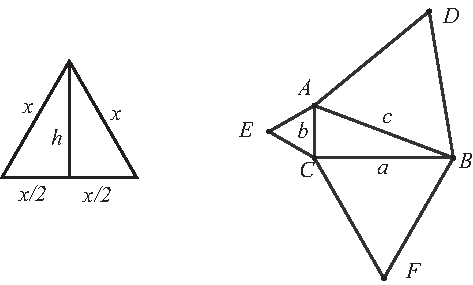
\includegraphics[width=\linewidth]{external/figps-pythag-triangle.pdf}
\end{image}%
\tcblower
\end{figureptx}%
%
\begin{enumerate}[font=\bfseries,label=(\alph*),ref=\alph*]
\item\label{x:task:exer-31-pythag-a}State the Pythagorean Theorem for right triangles.%
\par
The diagrams in \hyperref[x:figure:fig_for-exer-pythag]{Figure~{\xreffont\ref{x:figure:fig_for-exer-pythag}}, p.\,\pageref{x:figure:fig_for-exer-pythag}} will be used for the problems in this exercise.%
\item\label{x:task:exer-31-pythag-b}In the diagram on the left of \hyperref[x:figure:fig_for-exer-pythag]{Figure~{\xreffont\ref{x:figure:fig_for-exer-pythag}}, p.\,\pageref{x:figure:fig_for-exer-pythag}}, \(x\) is the length of a side of the equilateral triangle and \(h\) is the length of an altitude of the equilateral triangle. The labeling in the diagram shows the fact that the altitude intersects the base of the equilateral triangle at the midpoint of the base. Use the Pythagorean Theorem to prove that the area of this equilateral triangle is \(\dfrac{\sqrt{3}}{4}x^2\).%
\item\label{x:task:exer-31-pythag-c}In the diagram on the right of \hyperref[x:figure:fig_for-exer-pythag]{Figure~{\xreffont\ref{x:figure:fig_for-exer-pythag}}, p.\,\pageref{x:figure:fig_for-exer-pythag}}, \(\triangle ABC\) is a right triangle. In addition, there has been an equilateral triangle constructed on each side of this right triangle. Prove that the area of the equilateral triangle on the hypotenuse is equal to the sum of the areas of the equilateral triangles constructed on the other two sides of the right triangle.%
\end{enumerate}
\end{divisionexercise}%
\begin{divisionexercise}{19}{Evaluation of Proofs.}{}{x:exercise:exer_proofeval}%
This type of exercise will appear frequently in the book. In each case, there is a proposed proof of a proposition. However, the proposition may be true or may be false.%
\begin{itemize}[label=\textbullet]
\item{}If a proposition is false, the proposed proof is, of course, incorrect. In this situation, you are to find the error in the proof and then provide a counterexample showing that the proposition is false.%
\item{}If a proposition is true, the proposed proof may still be incorrect. In this case, you are to determine why the proof is incorrect and then write a correct proof using the writing guidelines that have been presented in this book.%
\item{}If a proposition is true and the proof is correct, you are to decide if the proof is well written or not. If it is well written, then you simply must indicate that this is an excellent proof and needs no revision. On the other hand, if the proof is not well written, then you must then revise the proof by writing it according to the guidelines presented in this text.%
\end{itemize}
%
\begin{enumerate}[font=\bfseries,label=(\alph*),ref=\alph*]
\item\label{x:task:prop-exer-even}%
\begin{descriptionlist}
\begin{dlinarrow}{Proposition}{g:li:idm827863064}%
If \(m\) is an even integer, then \(\left(5m + 4\right)\) is an even integer.%
\end{dlinarrow}%
\begin{dlinarrow}{Proof}{g:li:idm827859352}%
We see that \(5m + 4 = 10n + 4 = 2 \left(5n + 2 \right)\). Therefore, \(\left(5m + 4 \right)\) is an even integer.%
\end{dlinarrow}%
\end{descriptionlist}
%
\item\label{x:task:prop-exer-recipadd}%
\begin{descriptionlist}
\begin{dlinarrow}{Proposition}{g:li:idm827855256}%
For all real numbers \(x\) and \(y\), if \(x \ne y\), \(x > 0\), and \(y >0\), then \(\dfrac{x}{y} + \dfrac{y}{x} > 2\).%
\end{dlinarrow}%
\begin{dlinarrow}{Proof}{g:li:idm827859096}%
Since \(x\) and \(y\) are positive real numbers, \(xy\) is positive and we can multiply both sides of the inequality by \(xy\) to obtain%
\begin{align*}
\left( \frac{x}{y} + \frac{y}{x} \right) \cdot xy \amp > 2 \cdot xy\\
x^2 + y^2 \amp > 2xy\text{.}
\end{align*}
%
\par
By combining all terms on the left side of the inequality, we see that \(x^2 - 2xy + y^2 > 0\) and then by factoring the left side, we obtain \(\left( x - y \right)^2 > 0\). Since \(x \ne y\), \(\left(x - y \right) \ne 0\) and so \(\left( x - y \right)^2 > 0\). This proves that if \(x \ne y\), \(x > 0\), and \(y >0\), then \(\dfrac{x}{y} + \dfrac{y}{x} > 2\).%
\end{dlinarrow}%
\end{descriptionlist}
%
\item\label{x:task:prop-exer-divides}%
\begin{descriptionlist}
\begin{dlinarrow}{Proposition}{g:li:idm827851544}%
For all integers \(a\), \(b\), and \(c\), if \(a \mid \left( bc \right)\), then \(a \mid b\) or \(a \mid c\).%
\end{dlinarrow}%
\begin{dlinarrow}{Proof}{g:li:idm827839000}%
We assume that \(a\), \(b\), and \(c\) are integers and that \(a\) divides \(bc\). So, there exists an integer \(k\) such that \(bc = ka\).%
\par
We now factor \(k\) as \(k = mn\), where \(m\) and \(n\) are integers. We then see that%
\begin{equation*}
bc = mna\text{.}
\end{equation*}
%
\par
This means that \(b = ma\) or \(c = na\) and hence, \(a \mid b\) or \(a \mid c\).%
\end{dlinarrow}%
\end{descriptionlist}
%
\item\label{x:task:prop-exer-expo}%
\begin{descriptionlist}
\begin{dlinarrow}{Proposition}{g:li:idm827834264}%
For all positive integers \(a\), \(b\), and \(c\), \(\left( a^b \right)^c = a^{\left( b^c \right)}\).%
\end{dlinarrow}%
\begin{dlinarrow}{Proof}{g:li:idm827830424}%
This proposition is false as is shown by the following counterexample: If we let \(a = 2\), \(b = 3\), and \(c = 2\), then%
\begin{align*}
\left( a^b \right)^c \amp = a^{\left( b^c \right)}\\
\left( 2^3 \right)^2 \amp = 2^{\left( 3^2 \right)}\\
8^2 \amp = 2^9\\
64 \amp \ne 512\text{.}
\end{align*}
%
\end{dlinarrow}%
\end{descriptionlist}
%
\end{enumerate}
\end{divisionexercise}%
\begin{activity}{Congruence Modulo 6.}{g:activity:idm827826328}%
\begin{enumerate}[font=\bfseries,label=(\alph*),ref=\alph*]
\item\label{x:task:A_mod6-1}Find several integers that are congruent to 5 modulo 6 and then square each of these integers.%
\item\label{x:task:A_mod6-2}For each integer \(m\) from \hyperref[x:task:A_mod6-1]{Task~{\xreffont\ref{g:activity:idm827826328}}.{\xreffont\ref{x:task:A_mod6-1}}, p.\,\pageref{x:task:A_mod6-1}}, determine an integer \(k\) so that \(0 \leq k \lt 6\) and \(m^2 \equiv k \pmod 6\). What do you observe?%
\item\label{x:task:A_mod6-3}Based on the work in \hyperref[x:task:A_mod6-2]{Task~{\xreffont\ref{g:activity:idm827826328}}.{\xreffont\ref{x:task:A_mod6-2}}, p.\,\pageref{x:task:A_mod6-2}}, complete the following conjecture: \begin{quote}%
For each integer \(m\), if \(m \equiv 5 \pmod 6\), then \textellipsis{} .\end{quote}
%
\item{}Complete a know-show table for the conjecture in \hyperref[x:task:A_mod6-3]{Task~{\xreffont\ref{g:activity:idm827826328}}.{\xreffont\ref{x:task:A_mod6-3}}, p.\,\pageref{x:task:A_mod6-3}} or write a proof of the conjecture.%
\end{enumerate}
\end{activity}%
\begin{activity}{Pythagorean Triples.}{g:activity:idm827824792}%
\index{Pythagorean triple}%
\index{consecutive natural numbers}%
\index{natural numbers!consecutive}%
Three natural numbers \(a\), \(b\), and \(c\) with \(a \lt b \lt c\) are called a Pythagorean triple provided that \(a^2 + b^2 = c^2\). See \hyperref[x:activity:exer_pythag]{Activity~{\xreffont\ref{x:activity:exer_pythag}}, p.\,\pageref{x:activity:exer_pythag}} in \hyperref[x:section:S_1direct]{Section~{\xreffont\ref{x:section:S_1direct}}, p.\,\pageref{x:section:S_1direct}}. Three natural numbers are called \terminology{consecutive natural numbers} if they can be written in the form \(m\), \(m + 1\), and \(m + 2\), where \(m\) is a natural number.%
\begin{enumerate}[font=\bfseries,label=(\alph*),ref=\alph*]
\item{}Determine all Pythagorean triples consisting of three consecutive natural numbers. (State a theorem and prove it.)%
\item{}Determine all Pythagorean triples that can be written in the form \(m\), \(m + 7\), and \(m + 8\), where \(m\) is a natural number. State a theorem and prove it.%
\end{enumerate}
\end{activity}%
\end{exercises-subsection}
\end{sectionptx}
%
%
\typeout{************************************************}
\typeout{Section 3.2 More Methods of Proof}
\typeout{************************************************}
%
\begin{sectionptx}{More Methods of Proof}{}{More Methods of Proof}{}{}{x:section:S_moremethods}
%
%
\typeout{************************************************}
\typeout{Beginning Activity  Beginning Activity 2: Using the Contrapositive}
\typeout{************************************************}
%
\begin{worksheet-subsection}{Beginning Activity 2: Using the Contrapositive}{}{Beginning Activity 2: Using the Contrapositive}{}{}{x:worksheet:PA_attempt}
The following statement was proven in \hyperref[x:task:exer_x2odd]{Task~{\xreffont 3}.{\xreffont\ref{x:task:exer_x2odd}}, p.\,\pageref{x:task:exer_x2odd}} in \hyperref[x:section:S_1direct]{Section~{\xreffont\ref{x:section:S_1direct}}, p.\,\pageref{x:section:S_1direct}}. \begin{quote}%
If \(n\) is an odd integer, then \(n^2\) is an odd integer.\end{quote}
%
\par
Now consider the following proposition: \begin{quote}%
For each integer \(n\), if \(n^2\) is an odd integer, then \(n\) is an odd integer.\end{quote}
%
\begin{divisionexercise}{1}{}{}{g:exercise:idm827807128}%
After examining several examples, decide whether you think this proposition is true or false.%
\end{divisionexercise}%
\begin{divisionexercise}{2}{}{}{g:exercise:idm827810584}%
Try completing the following know-show~table for a direct proof of this proposition. The question is, ``Can we perform algebraic manipulations to get from the `know' portion of the table to the `show' portion of the table?'' Be careful with this! Remember that we are working with integers and we want to make sure that we can end up with an integer \(q\) as stated in Step \(Q1\).%
\end{divisionexercise}%
\begin{center}%
{\tabularfont%
\begin{tabular}{lll}
\multicolumn{1}{lB}{\textbf{Step}}&\multicolumn{1}{lB}{\textbf{Know}}&\textbf{Reason}\tabularnewline\hrulemedium
\multicolumn{1}{lB}{\(P\)}&\multicolumn{1}{lB}{\(n^2\) is an odd integer.}&Hypothesis\tabularnewline\hrulethin
\multicolumn{1}{lB}{\(P1\)}&\multicolumn{1}{lB}{\(\left( \exists k \in \Z \right) \left( n^2 = 2k + 1 \right)\)}&Definition of ``odd integer''\tabularnewline\hrulethin
\multicolumn{1}{cB}{\(\vdots\)}&\multicolumn{1}{cB}{\(\vdots\)}&\multicolumn{1}{c}{\(\vdots\)}\tabularnewline\hrulemedium
\multicolumn{1}{lB}{\(Q1\)}&\multicolumn{1}{lB}{\(\left( \exists q \in \Z \right) \left( n=2q \right)\)}&\tabularnewline\hrulethin
\multicolumn{1}{lB}{\(Q\)}&\multicolumn{1}{lB}{\(n\) is an odd integer.}&Definition of ``odd integer''\tabularnewline\hrulemedium
\multicolumn{1}{lB}{Step}&\multicolumn{1}{lB}{Show}&Reason
\end{tabular}
}%
\end{center}%
Recall that the contrapositive of the conditional statement \(P \to Q\) is the conditional statement \(\mynot Q \to \mynot P\), which is logically equivalent to the original conditional statement. (It might be a good idea to review \hyperref[x:worksheet:PA_converse]{Beginning Activity 2, p.\,\pageref{x:worksheet:PA_converse}} from \hyperref[x:section:S_logequiv]{Section~{\xreffont\ref{x:section:S_logequiv}}, p.\,\pageref{x:section:S_logequiv}}.) Consider the following proposition once again: \begin{quote}%
For each integer \(n\), if \(n^2\) is an odd integer, then \(n\) is an odd integer.\end{quote}
%
\begin{divisionexercise}{3}{}{}{x:exercise:PA_contrapositive2}%
Write the contrapositive of this conditional statement. Please note that ``not odd'' means ``even.'' (We have not proved this, but it can be proved using the Division Algorithm in \hyperref[x:section:S_divalgo]{Section~{\xreffont\ref{x:section:S_divalgo}}, p.\,\pageref{x:section:S_divalgo}}.)%
\end{divisionexercise}%
\begin{divisionexercise}{4}{}{}{x:exercise:PA_contrapositive3}%
Complete a know-show~table for the contrapositive statement from \hyperlink{x:exercise:PA_contrapositive2}{Exercise~{\xreffont 3}, p.\,\pageref{x:exercise:PA_contrapositive2}}.%
\end{divisionexercise}%
\begin{divisionexercise}{5}{}{}{g:exercise:idm827784984}%
By completing the proof in \hyperlink{x:exercise:PA_contrapositive3}{Exercise~{\xreffont 4}, p.\,\pageref{x:exercise:PA_contrapositive3}}, have you proven the given proposition? That is, have you proven that if \(n^2\) is an odd integer, then \(n\) is an odd integer? Explain.%
\end{divisionexercise}%
\end{worksheet-subsection}
%
%
\typeout{************************************************}
\typeout{Beginning Activity  Beginning Activity 2: A Biconditional Statement}
\typeout{************************************************}
%
\begin{worksheet-subsection}{Beginning Activity 2: A Biconditional Statement}{}{Beginning Activity 2: A Biconditional Statement}{}{}{x:worksheet:PA_biconditional}
\index{biconditional statement}%
\index{statement!biconditional}%
\begin{divisionexercise}{1}{}{}{x:exercise:PA_biconditional1}%
In \hyperref[x:task:exer_bicond]{Task~{\xreffont 4}.{\xreffont\ref{x:task:exer_bicond}}, p.\,\pageref{x:task:exer_bicond}} from \hyperref[x:section:S_logequiv]{Section~{\xreffont\ref{x:section:S_logequiv}}, p.\,\pageref{x:section:S_logequiv}}, we constructed a truth table to prove that the biconditional statement, \(P \leftrightarrow Q\), is logically equivalent to \(\left( {P \to Q} \right) \wedge \left( {Q \to P} \right)\). Complete this exercise if you have not already done so.%
\end{divisionexercise}%
\begin{divisionexercise}{2}{}{}{g:exercise:idm827773336}%
Suppose that we want to prove a biconditional statement of the form \(P \leftrightarrow Q\). Explain a method for completing this proof based on the logical equivalency in \hyperlink{x:exercise:PA_biconditional1}{Exercise~{\xreffont 1}, p.\,\pageref{x:exercise:PA_biconditional1}}.%
\end{divisionexercise}%
\begin{divisionexercise}{3}{}{}{g:exercise:idm827778584}%
Let \(n\) be an integer. Assume that we have completed the proofs of the following two statements:%
\begin{itemize}[label=\textbullet]
\item{}If \(n\) is an odd integer, then \(n^2\) is an odd integer.%
\item{}If \(n^2\) is an odd integer, then \(n\) is an odd integer.%
\end{itemize}
(See \hyperref[x:task:exer_x2odd]{Task~{\xreffont 3}.{\xreffont\ref{x:task:exer_x2odd}}, p.\,\pageref{x:task:exer_x2odd}} from \hyperref[x:section:S_1direct]{Section~{\xreffont\ref{x:section:S_1direct}}, p.\,\pageref{x:section:S_1direct}} and \hyperref[x:worksheet:PA_attempt]{Beginning Activity 1, p.\,\pageref{x:worksheet:PA_attempt}}.) Have we completed the proof of the following proposition? \begin{quote}%
For each integer \(n\), \(n\) is an odd integer if and only if \(n^2\) is an odd integer.\end{quote}
 Explain.%
\end{divisionexercise}%
\end{worksheet-subsection}
%
%
\typeout{************************************************}
\typeout{Subsection  Review of Direct Proofs}
\typeout{************************************************}
%
\begin{subsectionptx}{Review of Direct Proofs}{}{Review of Direct Proofs}{}{}{g:subsection:idm827767448}
\index{direct proof}%
\index{proof!direct}%
In \hyperref[x:section:S_1direct]{Section~{\xreffont\ref{x:section:S_1direct}}, p.\,\pageref{x:section:S_1direct}} and \hyperref[x:section:S_directproof]{Section~{\xreffont\ref{x:section:S_directproof}}, p.\,\pageref{x:section:S_directproof}}, we studied direct proofs of mathematical statements. Most of the statements we prove in mathematics are conditional statements that can be written in the form \(P \to Q\). A direct proof of a statement of the form \(P \to Q\) is based on the definition that a conditional statement can only be false when the hypothesis, \(P\), is true and the conclusion, \(Q\), is false. Thus, if the conclusion is true whenever the hypothesis is true, then the conditional statement must be true. So, in a direct proof,%
\begin{itemize}[label=\textbullet]
\item{}We start by assuming that \(P\) is true.%
\item{}From this assumption, we logically deduce that \(Q\) is true.%
\end{itemize}
We have used the so-called forward and backward method to discover how to logically deduce \(Q\) from the assumption that \(P\) is true.%
\end{subsectionptx}
%
%
\typeout{************************************************}
\typeout{Subsection  Proof Using the Contrapositive}
\typeout{************************************************}
%
\begin{subsectionptx}{Proof Using the Contrapositive}{}{Proof Using the Contrapositive}{}{}{g:subsection:idm827761304}
\index{contrapositive}%
\index{proof!contrapositive}%
As we saw in \hyperref[x:worksheet:PA_attempt]{Beginning Activity 1, p.\,\pageref{x:worksheet:PA_attempt}}, it is sometimes difficult to construct a direct proof of a conditional statement. This is one reason we studied logical equivalencies in \hyperref[x:section:S_logequiv]{Section~{\xreffont\ref{x:section:S_logequiv}}, p.\,\pageref{x:section:S_logequiv}}. Knowing that two expressions are logically equivalent tells us that if we prove one, then we have also proven the other. In fact, once we know the truth value of a statement, then we know the truth value of any other statement that is logically equivalent to it.%
\par
One of the most useful logical equivalencies in this regard is that a conditional statement \(P \to Q\) is logically equivalent to its contrapositive, \(\mynot Q \to \mynot P\). This means that if we prove the contrapositive of the conditional statement, then we have proven the conditional statement. The following are some important points to remember.%
\begin{itemize}[label=\textbullet]
\item{}A conditional statement is logically equivalent to its contrapositive.%
\item{}Use a direct proof to prove that \(\mynot Q \to \mynot P\) is true.%
\item{}Caution: One difficulty with this type of proof is in the formation of correct negations. (We need to be very careful doing this.)%
\item{}We might consider using a proof by contrapositive when the statements \(P\) and \(Q\) are stated as negations.%
\end{itemize}
%
\end{subsectionptx}
%
%
\typeout{************************************************}
\typeout{Subsection  Writing Guidelines}
\typeout{************************************************}
%
\begin{subsectionptx}{Writing Guidelines}{}{Writing Guidelines}{}{}{g:subsection:idm827751320}
\index{writing guidelines}%
One of the basic rules of writing mathematical proofs is to keep the reader informed. So when we prove a result using the contrapositive, we indicate this within the first few lines of the proof. For example,%
\begin{itemize}[label=\textbullet]
\item{}We will prove this theorem by proving its contrapositive.%
\item{}We will prove the contrapositive of this statement.%
\end{itemize}
%
\par
In addition, make sure the reader knows the status of every assertion that you make. That is, make sure you state whether an assertion is an assumption of the theorem, a previously proven result, a well-known result, or something from the reader's mathematical background. Following is a completed proof of a statement from \hyperref[x:worksheet:PA_attempt]{Beginning Activity 1, p.\,\pageref{x:worksheet:PA_attempt}}.%
\begin{theorem}{}{}{x:theorem:T_n2odd}%
For each integer \(n\), if \(n^2\) is an even integer, then \(n\) is an even integer.%
\end{theorem}
\begin{proof}{}{g:proof:idm827717256}
We will prove this result by proving the contrapositive of the statement, which is \begin{quote}%
For each integer \(n\), if \(n\) is an odd integer, then \(n^2\) is an odd integer.\end{quote}
%
\par
However, in \hyperref[x:theorem:T_xyodd]{Theorem~{\xreffont\ref{x:theorem:T_xyodd}}, p.\,\pageref{x:theorem:T_xyodd}}, we have already proven that if \(x\) and \(y\) are odd integers, then \(x \cdot y\) is an odd integer. So using \(x = y = n\), we can conclude that if \(n\) is an odd integer, then \(n \cdot n\), or \(n^2\), is an odd integer. We have thus proved the contrapositive of the theorem, and consequently, we have proved that if \(n^2\) is an even integer, then \(n\) is an even integer.%
\end{proof}
\end{subsectionptx}
%
%
\typeout{************************************************}
\typeout{Subsection  Using Other Logical Equivalencies}
\typeout{************************************************}
%
\begin{subsectionptx}{Using Other Logical Equivalencies}{}{Using Other Logical Equivalencies}{}{}{g:subsection:idm827716232}
As was noted in \hyperref[x:section:S_logequiv]{Section~{\xreffont\ref{x:section:S_logequiv}}, p.\,\pageref{x:section:S_logequiv}}, there are several different logical equivalencies. Fortunately, there are only a small number that we often use when trying to write proofs, and many of these are listed in \hyperref[x:theorem:T_logequiv]{Theorem~{\xreffont\ref{x:theorem:T_logequiv}}, p.\,\pageref{x:theorem:T_logequiv}} at the end of \hyperref[x:section:S_logequiv]{Section~{\xreffont\ref{x:section:S_logequiv}}, p.\,\pageref{x:section:S_logequiv}}. We will illustrate the use of one of these logical equivalencies with the following proposition: \begin{quote}%
For all real numbers \(a\) and \(b\), if \(a \ne 0\) and \(b \ne 0\), then \(ab \ne 0\).\end{quote}
%
\par
First, notice that the hypothesis and the conclusion of the conditional statement are stated in the form of negations. This suggests that we consider the contrapositive. Care must be taken when we negate the hypothesis since it is a conjunction. We use one of De Morgan's Laws as follows:%
\begin{equation*}
\mynot  \left( {a \ne 0\; \wedge \;b \ne 0} \right) \equiv \left( {a = 0} \right) \vee 
\left( {b = 0} \right)\text{.}
\end{equation*}
%
\begin{inlineexercise}{Using Another Logical Equivalency.}{x:exercise:pr_contrapositive}%
\begin{enumerate}[font=\bfseries,label=(\alph*),ref=\alph*]
\item\label{x:task:pr_contrapositive1}In English, write the contrapositive of, ``For all real numbers \(a\) and \(b\), if \(a \ne 0\) and \(b \ne 0\), then \(ab \ne 0\).''%
\space\hyperlink{g:solution:idm827704584-back}{[Solution]}\item\label{x:task:pr_contrapositive2}The contrapositive is a conditional statement in the form \(X \to \left( {Y \vee Z} \right)\). The difficulty is that there is not much we can do with the hypothesis \(\left( {ab = 0} \right)\) since we know nothing else about the real numbers \(a\) and \(b\). However, if we knew that \(a\) was not equal to zero, then we could multiply both sides of the equation \(ab = 0\) by \(\dfrac{1}{a}\). This suggests that we consider using the following logical equivalency based on a result in \hyperref[x:theorem:T_logequiv]{Theorem~{\xreffont\ref{x:theorem:T_logequiv}}, p.\,\pageref{x:theorem:T_logequiv}}:%
\begin{equation*}
X \to \left( {Y \vee Z} \right) \equiv \left( {X \wedge \mynot  Y} \right) \to Z\text{.}
\end{equation*}
%
\par
In English, use this logical equivalency to write a statement that is logically equivalent to the contrapositive from \hyperref[x:task:pr_contrapositive1]{Task~{\xreffont\ref{x:exercise:pr_contrapositive}}.{\xreffont\ref{x:task:pr_contrapositive1}}, p.\,\pageref{x:task:pr_contrapositive1}}.%
\space\hyperlink{g:solution:idm827697288-back}{[Solution]}\item{}The logical equivalency in \hyperref[x:task:pr_contrapositive2]{Task~{\xreffont\ref{x:exercise:pr_contrapositive}}.{\xreffont\ref{x:task:pr_contrapositive2}}, p.\,\pageref{x:task:pr_contrapositive2}} makes sense because if we are trying to prove \(Y \vee Z\), we only need to prove that at least one of \(Y\) or \(Z\) is true. So the idea is to prove that if \(Y\) is false, then \(Z\) must be true.%
\par
Use the ideas presented in the progress check to complete the proof of the following proposition. \begin{proposition}{}{}{x:proposition:P_abnotzero}%
For all real numbers \(a\) and \(b\), if \(a \ne 0\) and \(b \ne 0\), then \(ab \ne 0\).%
\end{proposition}
\begin{proof}{}{g:proof:idm827690376}
We will prove the contrapositive of this proposition, which is \begin{quote}%
For all real numbers \(a\) and \(b\), if \(ab = 0\), then \(a = 0\text{ or } b = 0\).\end{quote}
%
\par
This contrapositive, however, is logically equivalent to the following: \begin{quote}%
For all real numbers \(a\) and \(b\), if \(ab = 0\) and \(a \ne 0\), then \(b = 0\).\end{quote}
 To prove this, we let \(a\) and \(b\) be real numbers and assume that \(ab = 0\) and \(a \ne 0\). We can then multiply both sides of the equation \(ab = 0\) by \(\dfrac{1}{a}\). This gives%
\begin{equation*}
\text{Now complete the proof.}
\end{equation*}
%
\begin{equation*}
\vdots
\end{equation*}
%
\par
Therefore, \(b = 0\). This completes the proof of a statement that is logically equivalent to the contrapositive, and hence, we have proven the proposition.%
\end{proof}
%
\space\hyperlink{g:solution:idm827680648-back}{[Solution]}\end{enumerate}
\end{inlineexercise}%
\end{subsectionptx}
%
%
\typeout{************************************************}
\typeout{Subsection  Proofs of Biconditional Statements}
\typeout{************************************************}
%
\begin{subsectionptx}{Proofs of Biconditional Statements}{}{Proofs of Biconditional Statements}{}{}{g:subsection:idm827677064}
\index{proof!biconditional statement}%
\index{biconditional statement!proof of}%
In \hyperref[x:worksheet:PA_biconditional]{Beginning Activity 2, p.\,\pageref{x:worksheet:PA_biconditional}}, we used the following logical equivalency:%
\begin{equation*}
\left( {P \leftrightarrow Q} \right) \equiv \left( {P \to Q} \right) \wedge \left( {Q \to P} 
\right)\text{.}
\end{equation*}
This logical equivalency suggests one method for proving a biconditional statement written in the form ``\(P\) if and only if \(Q\).'' This method is to construct separate proofs of the two conditional statements \(P \to Q\) and \(Q \to P\). For example, since we have now proven each of the following:%
\begin{itemize}[label=\textbullet]
\item{}For each integer \(n\), if \(n\) is an even integer, then \(n^2\) is an even integer. (\hyperref[x:task:exer_x2odd]{Task~{\xreffont 3}.{\xreffont\ref{x:task:exer_x2odd}}, p.\,\pageref{x:task:exer_x2odd}} from \hyperlink{x:exercise:exer_evenoddmult}{Exercise~{\xreffont 3}, p.\,\pageref{x:exercise:exer_evenoddmult}} in \hyperref[x:section:S_1direct]{Section~{\xreffont\ref{x:section:S_1direct}}, p.\,\pageref{x:section:S_1direct}})%
\item{}For each integer \(n\), if \(n^2\) is an even integer, then \(n\) is an even integer. (\hyperref[x:theorem:T_n2odd]{Theorem~{\xreffont\ref{x:theorem:T_n2odd}}, p.\,\pageref{x:theorem:T_n2odd}})%
\end{itemize}
we can state the following theorem.%
\begin{theorem}{}{}{x:theorem:T_n2isodd}%
For each integer \(n\), \(n\) is an even integer if and only if \(n^2\) is an even integer.%
\end{theorem}
\end{subsectionptx}
%
%
\typeout{************************************************}
\typeout{Subsection  Writing Guidelines}
\typeout{************************************************}
%
\begin{subsectionptx}{Writing Guidelines}{}{Writing Guidelines}{}{}{g:subsection:idm827665672}
\index{writing guidelines}%
When proving a biconditional statement using the logical equivalency \(\left( {P \leftrightarrow Q} \right) \equiv \left( {P \to Q} \right) \wedge \left( {Q \to P} 
\right)\), we actually need to prove two conditional statements. The proof of each conditional statement can be considered as one of two parts of the proof of the biconditional statement. Make sure that the start and end of each of these parts is indicated clearly. This is illustrated in the proof of the following proposition. \begin{proposition}{}{}{x:proposition:P_iffexample}%
Let \(x \in \mathbb{R}\). The real number \(x\) equals 2 if and only if \(x^3 - 2x^2 + x = 2\).%
\end{proposition}
 \begin{proof}{}{g:proof:idm827656712}
We will prove this biconditional statement by proving the following two conditional statements:%
\begin{itemize}[label=\textbullet]
\item{}For each real number \(x\), if \(x\) equals 2 , then \(x^3 - 2x^2 + x = 2\).%
\item{}For each real number \(x\), if \(x^3 - 2x^2 + x = 2\), then \(x\) equals 2.%
\end{itemize}
%
\par
For the first part, we assume \(x = 2\) and prove that \(x^3  - 2x^2  + x = 2\). We can do this by substituting \(x = 2\) into the expression \(x^3  - 2x^2  + x\). This gives%
\begin{align*}
x^3  - 2x^2  + x \amp = 2^3  - 2\left( {2^2 } \right) + 2\\
\amp = 8 - 8 + 2\\
\amp =2\text{.}
\end{align*}
This completes the first part of the proof.%
\par
For the second part, we assume that \(x^3  - 2x^2  + x = 2\) and from this assumption, we will prove that \(x = 2\). We will do this by solving this equation for \(x\). To do so, we first rewrite the equation \(x^3  - 2x^2  + x = 2\) by subtracting 2 from both sides:%
\begin{equation*}
x^3  - 2x^2  + x - 2 = 0\text{.}
\end{equation*}
%
\par
We can now factor the left side of this equation by factoring an \(x^2\) from the first two terms and then factoring \(\left( {x - 2} \right)\) from the resulting two terms. This is shown below.%
\begin{align*}
x^3  - 2x^2  + x - 2 \amp = 0\\
x^2 \left( {x - 2} \right) + \left( {x - 2} \right) \amp = 0\\
\left( {x - 2} \right)\left( {x^2  + 1} \right) \amp = 0\text{.}
\end{align*}
Now, in the real numbers, if a product of two factors is equal to zero, then one of the factors must be zero. So this last equation implies that%
\begin{equation*}
x - 2 = 0\text{ or } x^2  + 1 = 0\text{.}
\end{equation*}
%
\par
The equation \(x^2 + 1 = 0\) has no real number solution. So since \(x\) is a real number, the only possibility is that \(x - 2 = 0\). From this we can conclude that \(x\) must be equal to 2.%
\par
Since we have now proven both conditional statements, we have proven that \(x = 2\) if and only if \(x^3 - 2x^2 + x = 2\).%
\end{proof}
%
\end{subsectionptx}
%
%
\typeout{************************************************}
\typeout{Subsection  Constructive Proofs}
\typeout{************************************************}
%
\begin{subsectionptx}{Constructive Proofs}{}{Constructive Proofs}{}{}{g:subsection:idm827654792}
\index{constructive proof}%
We all know how to solve an equation such as \(3x + 8 = 23\), where \(x\) is a real number. To do so, we first add \(-8\) to both sides of the equation and then divide both sides of the resulting equation by 3. Doing so, we obtain the following result:%
\begin{quote}%
If \(x\) is a real number and \(3x + 8 = 23\), then \(x = 5\).\end{quote}
Notice that the process of solving the equation actually does not prove that \(x = 5\) is a solution of the equation \(3x + 8 = 23\). This process really shows that if there is a solution, then that solution must be \(x = 5\). To show that this is a solution, we use the process of substituting \(5\) for \(x\) in the left side of the equation as follows: If \(x = 5\), then%
\begin{equation*}
3x + 8 = 3 \left( 5 \right) + 8 = 15 + 8 = 23\text{.}
\end{equation*}
%
\par
This proves that \(x = 5\) is a solution of the equation \(3x + 8 = 23\). Hence, we have proven that \(x = 5\) is the only real number solution of \(3x + 8 = 23\).%
\par
We can use this same process to show that any linear equation has a real number solution. An equation of the form%
\begin{equation*}
ax + b = c\text{,}
\end{equation*}
where \(a\), \(b\), and \(c\) are real numbers with \(a \ne 0\), is called a \terminology{linear equation in one variable}.%
\begin{proposition}{}{}{x:proposition:P_linearequation}%
If \(a\), \(b\), and \(c\) are real numbers with \(a \ne 0\), then the linear equation \(ax + b = c\) has exactly one real number solution, which is \(x = \dfrac{c - b}{a}\).%
\end{proposition}
\begin{proof}{}{g:proof:idm827638408}
Assume that \(a\), \(b\), and \(c\) are real numbers with \(a \ne 0\). We can solve the linear equation \(ax + b = c\) by adding \(-b\) to both sides of the equation and then dividing both sides of the resulting equation by \(a\) \(\left( \text{ since }  a \ne 0 \right)\), to obtain%
\begin{equation*}
x = \frac{c - b}{a}\text{.}
\end{equation*}
This shows that if there is a solution, then it must be \(x = \dfrac{c - b}{a}\). We also see that if \(x = \dfrac{c - b}{a}\), then%
\begin{align*}
ax + b \amp = a \left( \frac{c - b}{a} \right) + b\\
\amp = \left( c - b \right) + b\\
\amp = c\text{.}
\end{align*}
%
\par
Therefore, the linear equation \(ax + b = c\) has exactly one real number solution and the solution is \(x = \dfrac{c - b}{a}\).%
\end{proof}
\index{constructive proof}\index{proof!constructive}\index{existence theorem} The proof given for \hyperref[x:proposition:P_linearequation]{Proposition~{\xreffont\ref{x:proposition:P_linearequation}}, p.\,\pageref{x:proposition:P_linearequation}} is called a \terminology{constructive proof.} This is a technique that is often used to prove a so-called \terminology{existence theorem.} The objective of an existence theorem is to prove that a certain mathematical object exists. That is, the goal is usually to prove a statement of the form \begin{quote}%
There exists an \(x\) such that \(P( x )\).\end{quote}
 For a constructive proof of such a proposition, we actually name, describe, or explain how to construct some object in the universe that makes \(P( x )\) true. This is what we did in \hyperref[x:proposition:P_linearequation]{Proposition~{\xreffont\ref{x:proposition:P_linearequation}}, p.\,\pageref{x:proposition:P_linearequation}} since in the proof, we actually proved that \(\dfrac{c - b}{a}\) is a solution of the equation \(ax + b = c\). In fact, we proved that this is the only solution of this equation.%
\end{subsectionptx}
%
%
\typeout{************************************************}
\typeout{Subsection  Nonconstructive Proofs}
\typeout{************************************************}
%
\begin{subsectionptx}{Nonconstructive Proofs}{}{Nonconstructive Proofs}{}{}{g:subsection:idm827616776}
\index{existence theorem}%
\index{proof!non-constructive}%
Another type of proof that is often used to prove an existence theorem is the so-called \terminology{nonconstructive proof.} For this type of proof, we make an argument that an object in the universal set that makes \(P( x )\) true must exist but we never construct or name the object that makes \(P( x )\) true. The advantage of a constructive proof over a nonconstructive proof is that the constructive proof will yield a procedure or algorithm for obtaining the desired object.%
\par
\index{Intermediate Value Theorem} The proof of the \terminology{Intermediate Value Theorem} from calculus is an example of a nonconstructive proof. The Intermediate Value Theorem can be stated as follows: \begin{quote}%
If \(f\) is a continuous function on the closed interval \(\left[ {a,b} \right]\) and if \(q\) is any real number strictly between \(f( a )\) and \(f( b )\), then there exists a number \(c\) in the interval \(\left( {a,b} \right)\) such that \(f( c ) = q\).\end{quote}
%
\par
The Intermediate Value Theorem can be used to prove that a solution to some equations must exist. This is shown in the next example.%
\begin{example}{Using the Intermediate Value Theorem.}{g:example:idm827613448}%
Let \(x\) represent a real number. We will use the Intermediate Value Theorem to prove that the equation \(x^3 - x + 1 = 0\) has a real number solution.%
\par
To investigate solutions of the equation \(x^3  - x + 1 = 0\), we will use the function%
\begin{equation*}
f( x ) = x^3  - x + 1\text{.}
\end{equation*}
Notice that \(f( { - 2} ) =  - 5\) and that \(f( 0 ) = 1\). Since \(f ( -2 ) \lt  0\) and \(f ( 0 ) > 0\), the Intermediate Value Theorem tells us that there is a real number \(c\) between \(-2\) and \(0\) such that \(f( c ) = 0\). This means that there exists a real number \(c\) between \(-2\) and \(0\) such that%
\begin{equation*}
c^3  - c + 1 = 0\text{,}
\end{equation*}
and hence \(c\) is a real number solution of the equation \(x^3  - x + 1 = 0\). This proves that the equation \(x^3  - x + 1 = 0\) has at least one real number solution.%
\par
Notice that this proof does not tell us how to find the exact value of \(c\). It does, however, suggest a method for approximating the value of \(c\). This can be done by finding smaller and smaller intervals \(\left[ {a,\;b} \right]\) such that \(f( a )\) and \(f( b )\) have opposite signs.%
\end{example}
\end{subsectionptx}
%
%
\typeout{************************************************}
\typeout{Exercises  Exercises}
\typeout{************************************************}
%
\begin{exercises-subsection}{Exercises}{}{Exercises}{}{}{g:exercises:idm827606024}
\begin{divisionexercise}{1}{}{}{x:exercise:exer_ncubed}%
Let \(n\) be an integer. Prove each of the following:%
\begin{enumerate}[font=\bfseries,label=(\alph*),ref=\alph*]
\item\label{x:task:exer_ncubeda}If \(n\) is even, then \(n^3\) is even.%
\space\hyperlink{g:hint:idm827604360-back}{[Hint]}\item\label{x:task:exer_ncubedb}If \(n^3\) is even, then \(n\) is even.%
\space\hyperlink{g:hint:idm827594760-back}{[Hint]}\item{}The integer \(n\) is even if and only if \(n^3\) is an even integer.%
\space\hyperlink{g:hint:idm827591048-back}{[Hint]}\item{}The integer \(n\) is odd if and only if \(n^3\) is an odd integer.%
\space\hyperlink{g:hint:idm827590792-back}{[Hint]}\end{enumerate}
\end{divisionexercise}%
\begin{divisionexercise}{2}{}{}{x:exercise:exer_sec32-2}%
In \hyperref[x:section:S_directproof]{Section~{\xreffont\ref{x:section:S_directproof}}, p.\,\pageref{x:section:S_directproof}}, we defined congruence modulo \(n\) where \(n\) is a natural number. If \(a\) and \(b\) are integers, we will use the notation \(a \not\equiv b \pmod n\) to mean that \(a\) is not congruent to \(b\) modulo \(n\).%
\begin{enumerate}[font=\bfseries,label=(\alph*),ref=\alph*]
\item{}Write the contrapositive of the following conditional statement: \begin{quote}%
For all integers \(a\) and \(b\), if \(a \not\equiv 0 \pmod 6\) and \(b \not\equiv 0 \pmod 6\), then \(ab \not\equiv 0 \pmod 6\).\end{quote}
%
\space\hyperlink{g:answer:idm827582728-back}{[Answer]}\item{}Is this statement true or false? Explain.%
\end{enumerate}
\end{divisionexercise}%
\begin{divisionexercise}{3}{}{}{g:exercise:idm827577608}%
Complete the following.%
\begin{enumerate}[font=\bfseries,label=(\alph*),ref=\alph*]
\item{}Write the contrapositive of the following statement: For all positive real numbers \(a\) and \(b\), if \(\sqrt {ab} \ne \dfrac{{a + b}}{2}\), then \(a \ne b\).%
\space\hyperlink{g:answer:idm827580296-back}{[Answer]}\item{}Is this statement true or false? Prove the statement if it is true or provide a counterexample if it is false.%
\space\hyperlink{g:answer:idm827581064-back}{[Answer]}\end{enumerate}
\end{divisionexercise}%
\begin{divisionexercise}{4}{}{}{x:exercise:exer_sec32-4}%
Are the following statements true or false? Justify your conclusions.%
\begin{enumerate}[font=\bfseries,label=(\alph*),ref=\alph*]
\item{}For each \(a \in \Z\), if \(a \equiv 2 \pmod 5\), then \(a^2 \equiv 4 \pmod 5\).%
\space\hyperlink{g:answer:idm827572872-back}{[Answer]}\item{}For each \(a \in \Z\), if \(a^2 \equiv 4 \pmod 5\), then \(a \equiv 2 \pmod 5\).%
\space\hyperlink{g:answer:idm827568008-back}{[Answer]}\item{}For each \(a \in \Z\), \(a \equiv 2 \pmod 5\) if and only if \(a^2 \equiv 4 \pmod 5\).%
\space\hyperlink{g:answer:idm827564552-back}{[Answer]}\end{enumerate}
\end{divisionexercise}%
\begin{divisionexercise}{5}{}{}{x:exercise:exer_sec32-abeven}%
Is the following proposition true or false? \begin{quote}%
For all integers \(a\) and \(b\), if \(ab\) is even, then \(a\) is even or \(b\) is even.\end{quote}
 Justify your conclusion by writing a proof if the proposition is true or by providing a counterexample if it is false.%
\end{divisionexercise}%
\begin{divisionexercise}{6}{}{}{x:exercise:exer_sec32-congmod7}%
Consider the following proposition: For each integer \(a\), \(a \equiv 3 \pmod 7\) if and only if \(\left( a^2 + 5a \right) \equiv 3 \pmod 7\).%
\begin{enumerate}[font=\bfseries,label=(\alph*),ref=\alph*]
\item\label{x:task:exer_sec32-congmod7a}Write the proposition as the conjunction of two conditional statements.%
\space\hyperlink{g:answer:idm827563016-back}{[Answer]}\item{}Determine if the two conditional statements in \hyperref[x:task:exer_sec32-congmod7a]{Task~{\xreffont 6}.{\xreffont\ref{x:task:exer_sec32-congmod7a}}, p.\,\pageref{x:task:exer_sec32-congmod7a}} are true or false. If a conditional statement is true, write a proof, and if it is false, provide a counterexample.%
\space\hyperlink{g:answer:idm827554696-back}{[Answer]}\item{}Is the given proposition true or false? Explain.%
\space\hyperlink{g:answer:idm827542152-back}{[Answer]}\end{enumerate}
\end{divisionexercise}%
\begin{divisionexercise}{7}{}{}{x:exercise:exer_sec32-congmod8}%
Consider the following proposition: For each integer \(a\), \(a \equiv 2 \pmod 8\) if and only if \(\left(a^2 + 4a \right) \equiv 4 \pmod 8\).%
\begin{enumerate}[font=\bfseries,label=(\alph*),ref=\alph*]
\item{}Write the proposition as the conjunction of two conditional statements.%
\item{}Determine if the two conditional statements in Part~(a) are true or false. If a conditional statement is true, write a proof, and if it is false, provide a counterexample.%
\item{}Is the given proposition true or false? Explain.%
\end{enumerate}
\end{divisionexercise}%
\begin{divisionexercise}{8}{}{}{x:exercise:exer_sec32-6}%
For a right triangle, suppose that the hypotenuse has length \(c\) feet and the lengths of the sides are \(a\) feet and \(b\) feet.%
\begin{enumerate}[font=\bfseries,label=(\alph*),ref=\alph*]
\item{}What is a formula for the area of this right triangle? What is an isosceles triangle?%
\item{}State the Pythagorean Theorem for right triangles.%
\item{}Prove that the right triangle described above is an isosceles triangle if and only if the area of the right triangle is \(\dfrac{1}{4} c^2\).%
\space\hyperlink{g:answer:idm827536904-back}{[Answer]}\end{enumerate}
\end{divisionexercise}%
\begin{divisionexercise}{9}{}{}{x:exercise:exer_rational}%
\index{rational numbers}%
\index{irrational numbers}%
A real number  \(x\) is defined to be a \terminology{rational number} provided%
\begin{equation*}
\text{ there exist integers }  m  \text{ and }   n  \text{ with }   n \ne 0  
\text{ such that }   x = \frac{m}{n}\text{.}
\end{equation*}
A real number that is not a rational number is called an \terminology{irrational number.} It is known that if  \(x\)  is a positive rational number, then there exist positive integers \(m\) and \(n\) with \(n \ne 0\) such that \(x = \dfrac{m}{n}\). Is the following proposition true or false? Explain. \begin{quote}%
For each positive real number \(x\),  if  \(x\)  is irrational, then \(\sqrt x\) is irrational.\end{quote}
%
\space\hyperlink{g:answer:idm827525768-back}{[Answer]}\end{divisionexercise}%
\begin{divisionexercise}{10}{}{}{x:exercise:exer_sec32-8}%
Is the following proposition true or false? Justify your conclusion. \begin{quote}%
For each integer \(n\), \(n\) is even if and only if 4 divides \(n^2\).\end{quote}
%
\space\hyperlink{g:hint:idm827532296-back}{[Hint]}\end{divisionexercise}%
\begin{divisionexercise}{11}{}{}{g:exercise:idm827529352}%
Prove that for each integer \(a\), if \(a^2 - 1\) is even, then 4 divides \(a^2 - 1\).%
\end{divisionexercise}%
\begin{divisionexercise}{12}{}{}{g:exercise:idm827532680}%
Prove that for all integers \(a\) and \(m\), if \(a\) and \(m\) are the lengths of the sides of a right triangle and \(m + 1\) is the length of the hypotenuse, then \(a\) is an odd integer.%
\end{divisionexercise}%
\begin{divisionexercise}{13}{}{}{x:exercise:exer_rationalbetween}%
Prove the following proposition: \begin{quote}%
If \(p, q \in \mathbb{Q}\) with \(p \lt q\), then there exists an \(x \in \mathbb{Q}\) with \(p \lt x \lt q\).\end{quote}
%
\end{divisionexercise}%
\begin{divisionexercise}{14}{}{}{x:exercise:exer_existintegers}%
Are the following propositions true or false? Justify your conclusion.%
\begin{enumerate}[font=\bfseries,label=(\alph*),ref=\alph*]
\item{}There exist integers \(x\) and \(y\) such that \(4x + 6y = 2\).%
\item{}There exist integers \(x\) and \(y\) such that \(6x + 15y = 2\).%
\item{}There exist integers \(x\) and \(y\) such that \(6x + 15y = 9\).%
\end{enumerate}
\end{divisionexercise}%
\begin{divisionexercise}{15}{}{}{x:exercise:exer_IVT}%
Prove that there exists a real number \(x\) such that \(x^3 - 4x^2 = 7\).%
\space\hyperlink{g:hint:idm827516040-back}{[Hint]}\end{divisionexercise}%
\begin{divisionexercise}{16}{}{}{g:exercise:idm827511048}%
Let  \(y_1 , y_2 , y_3 , y_4\) be  real numbers. The \emph{mean}, \(\overline y\), of these four numbers is defined to be the sum of the four numbers divided by 4. That is,%
\begin{equation*}
\overline y  = \frac{{y_1  + y_2  + y_3  + y_4 }}{4}\text{.}
\end{equation*}
Prove that there exists a  \(y_i\) with  \(1 \leq i \leq 4\) such that \(y_i  \geq \overline y\).%
\space\hyperlink{g:hint:idm827510408-back}{[Hint]}\end{divisionexercise}%
\begin{divisionexercise}{17}{}{}{x:exercise:exer_sec32-16}%
Let \(a\) and \(b\) be natural numbers such that \(a^2 = b^3\). Prove each of the propositions in Parts (a) through (d). (The results of \hyperlink{x:exercise:exer_ncubed}{Exercise~{\xreffont 1}, p.\,\pageref{x:exercise:exer_ncubed}} and \hyperref[x:theorem:T_n2isodd]{Theorem~{\xreffont\ref{x:theorem:T_n2isodd}}, p.\,\pageref{x:theorem:T_n2isodd}} may be helpful.)%
\begin{enumerate}[font=\bfseries,label=(\alph*),ref=\alph*]
\item\label{x:task:exer_a2equalb3-a}If \(a\) is even, then 4 divides \(a\).%
\item{}If 4 divides \(a\), then 4 divides \(b\).%
\space\hyperlink{g:answer:idm827505032-back}{[Answer]}\item{}If 4 divides \(b\), then 8 divides \(a\).%
\item\label{x:task:exer_a2equalsb3-d}If \(a\) is even, then 8 divides \(a\).%
\item{}Give an example of natural numbers \(a\) and \(b\) such that \(a\) is even and \(a^2 = b^3\), but \(b\) is not divisible by 8.%
\end{enumerate}
\end{divisionexercise}%
\begin{divisionexercise}{18}{}{}{x:exercise:exer_sec32-equation17}%
Prove the following proposition: \begin{quote}%
Let \(a\) and \(b\) be integers with \(a \ne 0\). If \(a\) does not divide \(b\), then the equation \(ax^3 + bx + \left( b + a \right) = 0\) does not have a solution that is a natural number.\end{quote}
%
\space\hyperlink{g:hint:idm827490824-back}{[Hint]}\end{divisionexercise}%
\begin{divisionexercise}{19}{Evaluation of Proofs.}{}{g:exercise:idm827485960}%
See the instructions for \hyperlink{x:exercise:exer_proofeval}{Exercise~{\xreffont 19}, p.\,\pageref{x:exercise:exer_proofeval}} from \hyperref[x:section:S_directproof]{Section~{\xreffont\ref{x:section:S_directproof}}, p.\,\pageref{x:section:S_directproof}}.%
\begin{enumerate}[font=\bfseries,label=(\alph*),ref=\alph*]
\item\label{x:task:prop-eval32a}%
\begin{descriptionlist}
\begin{dlinarrow}{Proposition}{g:li:idm827483912}%
If \(m\) is an odd integer, then \(\left(m + 6\right)\) is an odd integer.%
\end{dlinarrow}%
\begin{dlinarrow}{Proof}{g:li:idm827487112}%
For \(m + 6\) to be an odd integer, there must exist an integer \(n\) such that%
\begin{equation*}
m + 6 = 2n + 1\text{.}
\end{equation*}
%
\par
By subtracting 6 from both sides of this equation, we obtain%
\begin{align*}
m \amp = 2n - 6 + 1\\
\amp = 2 \left(n - 3 \right) + 1\text{.}
\end{align*}
%
\par
By the closure properties of the integers, \(\left(n - 3 \right)\) is an integer, and hence, the last equation implies that \(m\) is an odd integer. This proves that if \(m\) is an odd integer, then \(m+6\) is an odd integer.%
\end{dlinarrow}%
\end{descriptionlist}
%
\item\label{x:task:prop-eval32b}%
\begin{descriptionlist}
\begin{dlinarrow}{Proposition}{g:li:idm827481224}%
For all integers \(m\) and \(n\), if \(mn\) is an even integer, then \(m\) is even or \(n\) is even.%
\end{dlinarrow}%
\begin{dlinarrow}{Proof}{g:li:idm827478024}%
For either \(m\) or \(n\) to be even, there exists an integer \(k\) such that \(m = 2k\) or \(n = 2k\). So if we multiply \(m\) and \(n\), the product will contain a factor of 2 and, hence, \(mn\) will be even.%
\end{dlinarrow}%
\end{descriptionlist}
%
\end{enumerate}
\end{divisionexercise}%
\begin{activity}{Using a Logical Equivalency.}{g:activity:idm827475208}%
Consider the following proposition: \begin{proposition}{}{}{x:proposition:prop-act1-32}%
For all integers \(a\) and \(b\), if 3 does not divide \(a\) and 3 does not divide \(b\), then 3 does not divide the product \(a \cdot b\).%
\end{proposition}
%
\begin{enumerate}[font=\bfseries,label=(\alph*),ref=\alph*]
\item{}Notice that the hypothesis of the proposition is stated as a conjunction of two negations ( ``3 does not divide \(a\) and 3 does not divide \(b\)''). Also, the conclusion is stated as the negation of a sentence ( ``3 does not divide the product \(a \cdot b\).''). This often indicates that we should consider using a proof of the contrapositive. If we use the symbolic form \(\left( {\mynot Q \wedge \mynot R} \right) \to \mynot P\) as a model for this proposition, what is \(P\), what is \(Q\), and what is \(R\)?%
\item{}Write a symbolic form for the contrapositive of \(\left( {\mynot Q \wedge \mynot R} \right) \to \mynot P\).%
\item{}Write the contrapositive of the proposition as a conditional statement in English.%
\par
We do not yet have all the tools needed to prove the proposition or its contrapositive.%
\item{}However, later in the text, we will learn that the following proposition is true. \begin{proposition}{Proposition X.}{}{x:proposition:propx-act1-32}%
Let \(a\) be an integer. If 3 does not divide \(a\), then there exist integers \(x\) and \(y\) such that \(3x + ay = 1\).%
\end{proposition}
%
\begin{enumerate}[font=\bfseries,label=(\roman*),ref=\theenumi.\roman*]
\item{}Find integers \(x\) and \(y\) guaranteed by \hyperref[x:proposition:propx-act1-32]{Proposition~{\xreffont\ref{x:proposition:propx-act1-32}}, p.\,\pageref{x:proposition:propx-act1-32}} when \(a = 5\).%
\item{}Find integers \(x\) and \(y\) guaranteed by \hyperref[x:proposition:propx-act1-32]{Proposition~{\xreffont\ref{x:proposition:propx-act1-32}}, p.\,\pageref{x:proposition:propx-act1-32}} when \(a = 2\).%
\item{}Find integers \(x\) and \(y\) guaranteed by \hyperref[x:proposition:propx-act1-32]{Proposition~{\xreffont\ref{x:proposition:propx-act1-32}}, p.\,\pageref{x:proposition:propx-act1-32}} when \(a = - 2\).%
\end{enumerate}
\item{}Assume that \hyperref[x:proposition:propx-act1-32]{Proposition~{\xreffont\ref{x:proposition:propx-act1-32}}, p.\,\pageref{x:proposition:propx-act1-32}} is true and use it to help construct a proof of the contrapositive of the given proposition. In doing so, you will most likely have to use the logical equivalency \(P \to \left( {Q \vee R} \right) \equiv \left( {P \wedge \mynot Q} \right) \to R\).%
\end{enumerate}
\end{activity}%
\end{exercises-subsection}
\end{sectionptx}
%
%
\typeout{************************************************}
\typeout{Section 3.3 Proof by Contradiction}
\typeout{************************************************}
%
\begin{sectionptx}{Proof by Contradiction}{}{Proof by Contradiction}{}{}{x:section:S_contradiction}
%
%
\typeout{************************************************}
\typeout{Beginning Activity  Beginning Activity 1: Proof by Contradiction}
\typeout{************************************************}
%
\begin{worksheet-subsection}{Beginning Activity 1: Proof by Contradiction}{}{Beginning Activity 1: Proof by Contradiction}{}{}{x:worksheet:PA_contradicton}
\index{proof!by contradiction}%
\index{tautology}%
\index{contradiction}%
In a \hyperref[x:assemblage:D_tautology]{Definition, p.\,\pageref{x:assemblage:D_tautology}} in \hyperref[x:section:S_2logop]{Section~{\xreffont\ref{x:section:S_2logop}}, p.\,\pageref{x:section:S_2logop}}, we defined a \terminology{tautology} to be a compound statement \(S\) that is true for all possible combinations of truth values of the component statements that are part of \(S\). We also defined \terminology{contradiction} to be a compound statement that is false for all possible combinations of truth values of the component statements that are part of \(S\).%
\par
That is, a tautology is necessarily true in all circumstances, and a contradiction is necessarily false in all circumstances.%
\begin{divisionexercise}{1}{}{}{g:exercise:idm827365016}%
Use truth tables to explain why \(\left( {P \vee \mynot P} \right)\) is a tautology and \(\left( {P \wedge \mynot P} \right)\) is a contradiction.%
\end{divisionexercise}%
\index{proof!by contradiction} Another method of proof that is frequently used in mathematics is a \terminology{proof by contradiction.} This method is based on the fact that a statement \(X\) can only be true or false (and not both). The idea is to prove that the statement \(X\) is true by showing that it cannot be false. This is done by assuming that \(X\) is false and proving that this leads to a contradiction. (The contradiction often has the form \(\left( {R \wedge \mynot R} \right)\), where \(R\) is some statement.) When this happens, we can conclude that the assumption that the statement \(X\) is false is incorrect and hence \(X\) cannot be false. Since it cannot be false, then \(X\) must be true.%
\par
A logical basis for the contradiction method of proof is the tautology%
\begin{equation*}
\left[ \mynot  X \to C \right] \to X\text{,}
\end{equation*}
where \(X\) is a statement and \(C\) is a contradiction. The following truth table establishes this tautology. \begin{center}%
{\tabularfont%
\begin{tabular}{ccccc}
\multicolumn{1}{cB}{\(X\)}&\multicolumn{1}{cC}{\(C\)}&\multicolumn{1}{cA}{\(\mynot X\)}&\multicolumn{1}{cB}{\(\mynot X \to C\)}&\((\mynot X \to C) \to X\)\tabularnewline\hrulethick
\multicolumn{1}{cB}{T}&\multicolumn{1}{cC}{F}&\multicolumn{1}{cA}{F}&\multicolumn{1}{cB}{T}&T\tabularnewline[0pt]
\multicolumn{1}{cB}{F}&\multicolumn{1}{cC}{F}&\multicolumn{1}{cA}{T}&\multicolumn{1}{cB}{F}&T
\end{tabular}
}%
\end{center}%
 This tautology shows that if \(\mynot X\) leads to a contradiction, then \(X\) must be true. The previous truth table also shows that the statement \(\mynot X \to C\) is logically equivalent to \(X\). This means that if we have proved that \(\mynot X\) leads to a contradiction, then we have proved statement \(X\). So if we want to prove a statement \(X\) using a proof by contradiction, we assume that \(\mynot X\) is true and show that this leads to a contradiction.%
\par
When we try to prove the conditional statement, ``If \(P\) then \(Q\)'' using a proof by contradiction, we must assume that \(P \to Q\) is false and show that this leads to a contradiction.%
\begin{divisionexercise}{2}{}{}{g:exercise:idm827348376}%
Use a truth table to show that \(\mynot \left( {P \to Q} \right)\) is logically equivalent to \(P \wedge \mynot Q\).%
\end{divisionexercise}%
The preceding logical equivalency shows that when we assume that \textbackslash{}mbox\textbraceleft{}\(P \to Q\)\textbraceright{} is false, we are assuming that \(P\) is true and \(Q\) is false. If we can prove that this leads to a contradiction, then we have shown that \(\mynot \left( {P \to Q} \right)\) is false and hence that \(P \to Q\) is true.%
\begin{divisionexercise}{3}{}{}{x:exercise:LA_contradiction2-1}%
Give a counterexample to show that the following statement is false. \begin{quote}%
For each real number \(x\), \(\dfrac{1}{x(1 - x)} \geq 4\).\end{quote}
%
\end{divisionexercise}%
\begin{divisionexercise}{4}{}{}{g:exercise:idm827342232}%
When a statement is false, it is sometimes possible to add an assumption that will yield a true statement. This is usually done by using a conditional statement. So instead of working with the statement in \hyperlink{x:exercise:LA_contradiction2-1}{Exercise~{\xreffont 3}, p.\,\pageref{x:exercise:LA_contradiction2-1}}, we will work with a related statement that is obtained by adding an assumption (or assumptions) to the hypothesis. \begin{quote}%
For each real number \(x\), if \(0 \lt x \lt 1\), then \(\dfrac{1}{x(1 - x)} \geq 4\).\end{quote}
 To begin a proof by contradiction for this statement, we need to assume the negation of the statement. To do this, we need to negate the entire statement, including the quantifier. Recall that the negation of a statement with a universal quantifier is a statement that contains an existential quantifier. (See \hyperref[x:theorem:T_negations]{Theorem~{\xreffont\ref{x:theorem:T_negations}}, p.\,\pageref{x:theorem:T_negations}}.) With this in mind, carefully write down all assumptions made at the beginning of a proof by contradiction for this statement.%
\end{divisionexercise}%
\end{worksheet-subsection}
%
%
\typeout{************************************************}
\typeout{Beginning Activity  Beginning Activity 2: Constructing a Proof by Contradiction}
\typeout{************************************************}
%
\begin{worksheet-subsection}{Beginning Activity 2: Constructing a Proof by Contradiction}{}{Beginning Activity 2: Constructing a Proof by Contradiction}{}{}{x:worksheet:LA_contradicton2}
Consider the following proposition: \begin{proposition}{}{}{x:proposition:prop-contradictionba}%
For all real numbers \(x\) and \(y\), if \(x \ne y\), \(x > 0,\text{ and } y > 0\), then \(\dfrac{x}{y} + \dfrac{y}{x} > 2\).%
\end{proposition}
 To start a proof by contradiction, we assume that this statement is false; that is, we assume the negation is true. Because this is a statement with a universal quantifier, we assume that there exist real numbers \(x\) and \(y\) such that \(x \ne y\), \(x > 0, y > 0\) and that \(\dfrac{x}{y} + \dfrac{y}{x} \leq 2\). (Notice that the negation of the conditional sentence is a conjunction.)%
\par
For this proof by contradiction, we will only work with the know column of a know-show table. This is because we do not have a specific goal. The goal is to obtain some contradiction, but we do not know ahead of time what that contradiction will be. Using our assumptions, we can perform algebraic operations on the inequality%
\begin{equation}
\frac{x}{y} + \frac{y}{x} \leq 2\label{x:men:ineq_contradict1}
\end{equation}
until we obtain a contradiction.%
\begin{divisionexercise}{1}{}{}{g:exercise:idm827334552}%
Try the following algebraic operations on the inequality in \hyperref[x:men:ineq_contradict1]{({\xreffont\ref{x:men:ineq_contradict1}})}. First, multiply both sides of the inequality by \(xy\), which is a positive real number since \(x > 0\) and \(y > 0\). Then, subtract \(2xy\) from both sides of this inequality and finally, factor the left side of the resulting inequality.%
\end{divisionexercise}%
\begin{divisionexercise}{2}{}{}{g:exercise:idm827336088}%
Explain why the last inequality you obtained leads to a contradiction.%
\end{divisionexercise}%
By obtaining a contradiction, we have proved that the proposition cannot be false, and hence, must be true.%
\end{worksheet-subsection}
%
%
\typeout{************************************************}
\typeout{Subsection  Writing Guidelines: Keep the Reader Informed}
\typeout{************************************************}
%
\begin{subsectionptx}{Writing Guidelines: Keep the Reader Informed}{}{Writing Guidelines: Keep the Reader Informed}{}{}{g:subsection:idm827329816}
\index{writing guidelines}%
A very important piece of information about a proof is the method of proof to be used. So when we are going to prove a result using the contrapositive or a proof by contradiction, we indicate this at the start of the proof.%
\begin{itemize}[label=\textbullet]
\item{}We will prove this result by proving the contrapositive of the statement.%
\item{}We will prove this statement using a proof by contradiction.%
\item{}We will use a proof by contradiction.%
\end{itemize}
%
\par
We have discussed the logic behind a proof by contradiction in the beginning activities for this section. The basic idea for a proof by contradiction of a proposition is to assume the proposition is false and show that this leads to a contradiction. We can then conclude that the proposition cannot be false, and hence, must be true. When we assume a proposition is false, we are, in effect, assuming that its negation is true. This is one reason why it is so important to be able to write negations of propositions quickly and correctly. We will illustrate the process with the proposition discussed in \hyperref[x:worksheet:PA_contradicton]{Beginning Activity 1, p.\,\pageref{x:worksheet:PA_contradicton}}.%
\begin{proposition}{}{}{g:proposition:idm827324056}%
For each real number \(x\), if \(0 \lt x \lt 1\), then \(\dfrac{1}{x(1 - x)} \geq 4\).%
\end{proposition}
\begin{proof}{}{g:proof:idm827325208}
We will use a proof by contradiction. So we assume that the proposition is false, or that there exists a real number \(x\) such that \(0 \lt  x \lt  1\) and%
\begin{equation}
\dfrac{1}{x(1 - x)} \lt  4\text{.}\label{x:men:eq_contradiction1}
\end{equation}
%
\par
We note that since \(0 \lt  x \lt  1\), we can conclude that \(x > 0\) and that \((1 - x)>0\). Hence, \(x(1 - x) >0\) and if we multiply both sides of inequality \hyperref[x:men:eq_contradiction1]{({\xreffont\ref{x:men:eq_contradiction1}})} by \(x(1 - x)\), we obtain%
\begin{equation*}
1 \lt  4x(1 - x)\text{.}
\end{equation*}
%
\par
We can now use algebra to rewrite the last inequality as follows:%
\begin{align*}
1 \amp \lt  4x - 4x^2\\
4x^2 - 4x + 1 \amp \lt  0\\
(2x - 1)^2 \amp \lt  0
\end{align*}
%
\par
However, \((2x - 1)\) is a real number and the last inequality says that a real number squared is less than zero. This is a contradiction since the square of any real number must be greater than or equal to zero. Hence, the proposition cannot be false, and we have proved that for each real number \(x\), if \(0 \lt x \lt 1\), then \(\dfrac{1}{x(1 - x)} \geq 4\).%
\end{proof}
\begin{inlineexercise}{Starting a Proof by Contradiction.}{x:exercise:pr_start-con}%
One of the most important parts of a proof by contradiction is the very first part, which is to state the assumptions that will be used in the proof by contradiction. This usually involves writing a clear negation of the proposition to be proven. Review De Morgan's Laws and the negation of a conditional statement in \hyperref[x:section:S_logequiv]{Section~{\xreffont\ref{x:section:S_logequiv}}, p.\,\pageref{x:section:S_logequiv}}. (See \hyperref[x:theorem:T_logequiv]{Theorem~{\xreffont\ref{x:theorem:T_logequiv}}, p.\,\pageref{x:theorem:T_logequiv}}.) Also, review \hyperref[x:theorem:T_negations]{Theorem~{\xreffont\ref{x:theorem:T_negations}}, p.\,\pageref{x:theorem:T_negations}} and then write a negation of each of the following statements. (Remember that a real number is ``not irrational'' means that the real number is rational.)%
\begin{enumerate}[font=\bfseries,label=(\alph*),ref=\alph*]
\item{}For each real number \(x\), if \(x\) is irrational, then \(\sqrt[3]{x}\) is irrational.%
\space\hyperlink{g:solution:idm827312280-back}{[Solution]}\item{}For each real number \(x\), \(\left(x + \sqrt{2} \right)\) is irrational or \(\left(-x + \sqrt{2} \right)\) is irrational.%
\space\hyperlink{g:solution:idm827308824-back}{[Solution]}\item{}For all integers \(a\) and \(b\), if 5 divides \(ab\), then 5 divides \(a\) or 5 divides \(b\).%
\space\hyperlink{g:solution:idm827304216-back}{[Solution]}\item{}For all real numbers \(a\) and \(b\), if \(a > 0\) and \(b > 0\), then \(\dfrac{2}{a} + \dfrac{2}{b} \ne \dfrac{4}{a + b}\).%
\space\hyperlink{g:solution:idm827296280-back}{[Solution]}\end{enumerate}
\end{inlineexercise}%
\end{subsectionptx}
%
%
\typeout{************************************************}
\typeout{Subsection  Important Note}
\typeout{************************************************}
%
\begin{subsectionptx}{Important Note}{}{Important Note}{}{}{g:subsection:idm827302168}
A proof by contradiction is often used to prove a conditional statement \(P \to Q\) when a direct proof has not been found and it is relatively easy to form the negation of the proposition. The advantage of a proof by contradiction is that we have an additional assumption with which to work (since we assume not only \(P\) but also \(\mynot Q\)). The disadvantage is that there is no well-defined goal to work toward. The goal is simply to obtain some contradiction. There usually is no way of telling beforehand what that contradiction will be, so we have to stay alert for a possible absurdity. Thus, when we set up a know-show table for a proof by contradiction, we really only work with the know portion of the table.%
\begin{inlineexercise}{Exploration and a Proof by Contradiction.}{x:exercise:pr_exploreproof}%
Consider the following proposition: \begin{quote}%
For each integer \(n\), if \(n \equiv 2 \pmod 4\), then \(n\not \equiv 3 \pmod 6\).\end{quote}
%
\begin{enumerate}[font=\bfseries,label=(\alph*),ref=\alph*]
\item\label{x:task:pr_exploreproof1}Determine at least five different integers that are congruent to 2 modulo 4, and determine at least five different integers that are congruent to 3 modulo 6. Are there any integers that are in both of these lists?%
\space\hyperlink{g:solution:idm827290904-back}{[Solution]}\item{}For this proposition, why does it seem reasonable to try a proof by contradiction?%
\space\hyperlink{g:solution:idm827291672-back}{[Solution]}\item{}For this proposition, state clearly the assumptions that need to be made at the beginning of a proof by contradiction, and then use a proof by contradiction to prove this proposition.%
\space\hyperlink{g:solution:idm827293336-back}{[Solution]}\end{enumerate}
\end{inlineexercise}%
\end{subsectionptx}
%
%
\typeout{************************************************}
\typeout{Subsection  Proving that Something Does Not Exist}
\typeout{************************************************}
%
\begin{subsectionptx}{Proving that Something Does Not Exist}{}{Proving that Something Does Not Exist}{}{}{g:subsection:idm827284632}
In mathematics, we sometimes need to prove that something does not exist or that something is not possible. Instead of trying to construct a direct proof, it is sometimes easier to use a proof by contradiction so that we can assume that the something exists. For example, suppose we want to prove the following proposition:%
\begin{proposition}{}{}{x:proposition:prop_persquare}%
For all integers \(x\) and \(y\), if \(x\) and \(y\) are odd integers, then there does not exist an integer \(z\) such that \(x^2 + y^2 = z^2\).%
\end{proposition}
Notice that the conclusion involves trying to prove that an integer with a certain property does not exist. If we use a proof by contradiction, we can assume that such an integer \(z\) exists. This gives us more with which to work.%
\begin{inlineexercise}{}{x:exercise:prog_persquare}%
Complete the following proof of \hyperref[x:proposition:prop_persquare]{Proposition~{\xreffont\ref{x:proposition:prop_persquare}}, p.\,\pageref{x:proposition:prop_persquare}}:%
\par
Proof: We will use a proof by contradiction. So we assume that there exist integers \(x\) and \(y\) such that \(x\) and \(y\) are odd and there exists an integer \(z\) such that \(x^2 + y^2 = z^2\). Since \(x\) and \(y\) are odd, there exist integers \(m\) and \(n\) such that \(x = 2m + 1\) and \(y = 2n + 1\).%
\begin{enumerate}[font=\bfseries,label=(\alph*),ref=\alph*]
\item{}Use the assumptions that \(x\) and \(y\) are odd to prove that \(x^2 + y^2\) is even and hence, \(z^2\) is even. (See \hyperref[x:theorem:T_n2odd]{Theorem~{\xreffont\ref{x:theorem:T_n2odd}}, p.\,\pageref{x:theorem:T_n2odd}}.)%
\space\hyperlink{g:solution:idm827268376-back}{[Solution]}\item{}We can now conclude that \(z\) is even. (See \hyperref[x:theorem:T_n2odd]{Theorem~{\xreffont\ref{x:theorem:T_n2odd}}, p.\,\pageref{x:theorem:T_n2odd}}.) So there exists an integer \(k\) such that \(z = 2k\). If we substitute for \(x\), \(y\), and \(z\) in the equation \(x^2 + y^2 = z^2\), we obtain%
\begin{equation*}
(2m + 1)^2 + (2n + 1)^2 = (2k)^2\text{.}
\end{equation*}
%
\par
Use the previous equation to obtain a contradiction.%
\space\hyperlink{g:solution:idm827264664-back}{[Solution]}\end{enumerate}
\end{inlineexercise}%
\end{subsectionptx}
%
%
\typeout{************************************************}
\typeout{Subsection  Rational and Irrational Numbers}
\typeout{************************************************}
%
\begin{subsectionptx}{Rational and Irrational Numbers}{}{Rational and Irrational Numbers}{}{}{g:subsection:idm827255960}
One of the most important ways to classify real numbers is as a rational number or an irrational number. Following is the definition of rational (and irrational) numbers given in \hyperlink{x:exercise:exer_rational}{Exercise~{\xreffont 9}, p.\,\pageref{x:exercise:exer_rational}} from \hyperref[x:section:S_moremethods]{Section~{\xreffont\ref{x:section:S_moremethods}}, p.\,\pageref{x:section:S_moremethods}}.%
\begin{assemblage}{Definition.}{x:assemblage:D_rational}%
A real number \(x\) is defined to be a \terminology{rational number} provided that there exist integers \(m\) and \(n\) with \(n \ne 0\) such that \(x = \dfrac{m}{n}\). A real number that is not a rational number is called an \terminology{irrational number}.%
\end{assemblage}
This may seem like a strange distinction because most people are quite familiar with the rational numbers (fractions) but the irrational numbers seem a bit unusual. However, there are many irrational numbers such as \(\sqrt{2}\), \(\sqrt{3}\), \(\sqrt[3]{2}\), \(\pi\), and the number \(e\). We are discussing these matters now because we will soon prove that \(\sqrt{2}\) is irrational in \hyperref[x:theorem:T_squareroot2]{Theorem~{\xreffont\ref{x:theorem:T_squareroot2}}, p.\,\pageref{x:theorem:T_squareroot2}}.%
\par
We use the symbol \(\Q\) to stand for the set of rational numbers. There is no standard symbol for the set of irrational numbers. Perhaps one reason for this is because of the closure properties of the rational numbers. We introduced closure properties in \hyperref[x:section:S_1prop]{Section~{\xreffont\ref{x:section:S_1prop}}, p.\,\pageref{x:section:S_1prop}}, and the rational numbers \(\Q\) are closed under addition, subtraction, multiplication, and division by nonzero rational numbers. This means that if \(x, y \in \Q\), then%
\begin{itemize}[label=\textbullet]
\item{}\(x + y\), \(x - y\), and \(xy\) are in \(\Q\); and%
\item{}If \(y \ne 0\), then \(\dfrac{x}{y}\) is in \(\Q\).%
\end{itemize}
%
\par
The basic reasons for these facts are that if we add, subtract, multiply, or divide two fractions, the result is a fraction. One reason we do not have a symbol for the irrational numbers is that the irrational numbers are not closed under these operations. For example, we will prove that \(\sqrt{2}\) is irrational in \hyperref[x:theorem:T_squareroot2]{Theorem~{\xreffont\ref{x:theorem:T_squareroot2}}, p.\,\pageref{x:theorem:T_squareroot2}}. We then see that%
\begin{equation*}
\sqrt{2} \sqrt{2} = 2  \text{ and }   \frac{\sqrt{2}}{\sqrt{2}} = 1\text{,}
\end{equation*}
which shows that the product of irrational numbers can be rational and the quotient of irrational numbers can be rational.%
\par
It is also important to realize that every integer is a rational number since any integer can be written as a fraction. For example, we can write \(3 = \dfrac{3}{1}\). In general, if \(n \in \Z\), then \(n = \dfrac{n}{1}\), and hence, \(n \in \Q\).%
\par
Because the rational numbers are closed under the standard operations and the definition of an irrational number simply says that the number is not rational, we often use a proof by contradiction to prove that a number is irrational. This is illustrated in the next proposition.%
\begin{proposition}{}{}{g:proposition:idm827240472}%
For all real numbers \(x\) and \(y\), if \(x\) is rational and \(x \ne 0\) and \(y\) is irrational, then \(x \cdot y\) is irrational.%
\end{proposition}
\begin{proof}{}{g:proof:idm827231640}
We will use a proof by contradiction. So we assume that there exist real numbers \(x\) and \(y\) such that \(x\) is rational, \(x \ne 0\), \(y\) is irrational, and \(x \cdot y\) is rational. Since \(x \ne 0\), we can divide by \(x\), and since the rational numbers are closed under division by nonzero rational numbers, we know that \(\dfrac{1}{x} \in \Q\). We now know that \(x \cdot y\) and \(\dfrac{1}{x}\) are rational numbers and since the rational numbers are closed under multiplication, we conclude that%
\begin{equation*}
\frac{1}{x} \cdot \left( xy \right) \in \Q\text{.}
\end{equation*}
%
\par
However, \(\dfrac{1}{x} \cdot \left( xy \right) = y\) and hence, \(y\) must be a rational number. Since a real number cannot be both rational and irrational, this is a contradiction to the assumption that \(y\) is irrational. We have therefore proved that for all real numbers \(x\) and \(y\), if \(x\) is rational and \(x \ne 0\) and \(y\) is irrational, then \(x \cdot y\) is irrational.%
\end{proof}
\end{subsectionptx}
%
%
\typeout{************************************************}
\typeout{Subsection  The Square Root of 2 Is an Irrational Number}
\typeout{************************************************}
%
\begin{subsectionptx}{The Square Root of 2 Is an Irrational Number}{}{The Square Root of 2 Is an Irrational Number}{}{}{g:subsection:idm827223832}
The proof that the square root of 2 is an irrational number is one of the classic proofs in mathematics, and every mathematics student should know this proof. This is why we will be doing some preliminary work with rational numbers and integers before completing the proof. The theorem we will be proving can be stated as follows:%
\begin{theorem}{}{}{x:theorem:T_squareroot2}%
If \(r\) is a real number such that \(r^2 = 2\), then \(r\) is an irrational number.%
\end{theorem}
This is stated in the form of a conditional statement, but it basically means that \(\sqrt 2\) is irrational (and that \(- \sqrt 2\) is irrational). That is, \(\sqrt 2\) cannot be written as a quotient of integers with the denominator not equal to zero.%
\par
In order to complete this proof, we need to be able to work with some basic facts that follow about rational numbers and even integers.%
\begin{enumerate}
\item{}Each integer \(m\) is a rational number since \(m\) can be written as \(m = \dfrac{m}{1}\).%
\item\label{x:li:LA_learn33-eq2}{}\hypertarget{x:li:LA_learn33-eq2}{}Notice that \(\dfrac{2}{3} = \dfrac{4}{6}\), since%
\begin{equation*}
\frac{4}{6} = \frac{2 \cdot 2}{3 \cdot 2} = \frac{2}{2} \cdot \frac{2}{3} = 
\frac{2}{3}
\end{equation*}
We can also show that%
\begin{equation*}
\dfrac{15}{12} = \dfrac{5}{4}, \dfrac{10}{-8} 
= \dfrac{-5}{4}, \text{ and } \dfrac{-30}{-16} = \dfrac{15}{8}
\end{equation*}
%
\item{}\hyperlink{x:li:LA_learn33-eq2}{Item~{\xreffont 2}, p.\,\pageref{x:li:LA_learn33-eq2}} was included to illustrate the fact that a rational number can be written as a fraction in ``lowest terms'' with a positive denominator. This means that any rational number can be written as a quotient \(\dfrac{m}{n}\), where \(m\) and \(n\) are integers, \(n > 0\), and \(m\) and \(n\) have no common factor greater than 1.%
\par
If \(n\) is an integer and \(n^2\) is even, what can be concluded about \(n\). Refer to \hyperref[x:theorem:T_n2odd]{Theorem~{\xreffont\ref{x:theorem:T_n2odd}}, p.\,\pageref{x:theorem:T_n2odd}}.%
\end{enumerate}
%
\par
In a proof by contradiction of a conditional statement \(P \to Q\), we assume the negation of this statement or \(P \wedge \mynot Q\). So in a proof by contradiction of \hyperref[x:theorem:T_squareroot2]{Theorem~{\xreffont\ref{x:theorem:T_squareroot2}}, p.\,\pageref{x:theorem:T_squareroot2}}, we will assume that \(r\) is a real number, \(r^2 = 2\), and \(r\) is not irrational (that is, \(r\) is rational).%
\begin{theorem}{}{}{g:theorem:idm827207448}%
If \(r\) is a real number such that \(r^2 = 2\), then \(r\) is an irrational number.%
\end{theorem}
\begin{proof}{}{g:proof:idm827206936}
We will use a proof by contradiction. So we assume that the statement of the theorem is false. That is, we assume that \begin{quote}%
\(r\) is a real number, \(r^2 = 2\), and \(r\) is a rational number.\end{quote}
%
\par
Since \(r\) is a rational number, there exist integers \(m\) and \(n\) with \(n > 0\) such that%
\begin{equation*}
r = \frac{m}{n}
\end{equation*}
and \(m\) and \(n\) have no common factor greater than 1. We will obtain a contradiction by showing that \(m\) and \(n\) must both be even. Squaring both sides of the last equation and using the fact that \(r^2 = 2\), we obtain%
\begin{align}
2 \amp = \frac{{m^2 }}{{n^2 }} \amp\label{g:mrow:idm827202968}\\
m^2  \amp = 2n^2\label{x:mrow:eq_3h}
\end{align}
%
\par
Equation \hyperref[x:mrow:eq_3h]{({\xreffont\ref{x:mrow:eq_3h}})} implies that \(m^2\) is even, and hence, by \hyperref[x:theorem:T_n2odd]{Theorem~{\xreffont\ref{x:theorem:T_n2odd}}, p.\,\pageref{x:theorem:T_n2odd}}, \(m\) must be an even integer. This means that there exists an integer \(p\) such that \(m = 2p\). We can now substitute this into equation \hyperref[x:mrow:eq_3h]{({\xreffont\ref{x:mrow:eq_3h}})}, which gives%
\begin{align}
\left( {2p} \right)^2  \amp = 2n^2 \amp \notag\\
4p^2  \amp = 2n^2\label{x:mrow:eq_3i}
\end{align}
%
\par
We can divide both sides of equation \hyperref[x:mrow:eq_3i]{({\xreffont\ref{x:mrow:eq_3i}})} by 2 to obtain \(n^2 = 2p^2\). Consequently, \(n^2\) is even and we can once again use \hyperref[x:theorem:T_n2odd]{Theorem~{\xreffont\ref{x:theorem:T_n2odd}}, p.\,\pageref{x:theorem:T_n2odd}} to conclude that \(n\) is an even integer.%
\par
We have now established that both \(m\) and \(n\) are even. This means that 2 is a common factor of \(m\) and \(n\), which contradicts the assumption that \(m\) and \(n\) have no common factor greater than 1. Consequently, the statement of the theorem cannot be false, and we have proved that if \(r\) is a real number such that \(r^2 = 2\), then \(r\) is an irrational number.%
\end{proof}
\end{subsectionptx}
%
%
\typeout{************************************************}
\typeout{Exercises  Exercises}
\typeout{************************************************}
%
\begin{exercises-subsection}{Exercises}{}{Exercises}{}{}{g:exercises:idm827192728}
\begin{divisionexercise}{1}{}{}{x:exercise:exer_sec33-1}%
This exercise is intended to provide another rationale as to why a proof by contradiction works. Suppose that we are trying to prove that a statement \(P\) is true. Instead of proving this statement, assume that we prove that the conditional statement ``If \(\mynot P\), then \(C\)'' is true, where \(C\) is some contradiction. Recall that a contradiction is a statement that is always false.%
\begin{enumerate}[font=\bfseries,label=(\alph*),ref=\alph*]
\item\label{x:task:exer_contradictionproof}In symbols, write a statement that is a disjunction and that is logically equivalent to \(\mynot P \to C\).%
\space\hyperlink{g:answer:idm827188120-back}{[Answer]}\item{}Since we have proven that \(\mynot P \to C\) is true, then the disjunction in \hyperref[x:task:exer_contradictionproof]{Task~{\xreffont 1}.{\xreffont\ref{x:task:exer_contradictionproof}}, p.\,\pageref{x:task:exer_contradictionproof}} must also be true. Use this to explain why the statement \(P\) must be true.%
\item{}Now explain why \(P\) must be true if we prove that the negation of \(P\) implies a contradiction.%
\end{enumerate}
\end{divisionexercise}%
\begin{divisionexercise}{2}{}{}{x:exercise:exer_sec32-truefalse}%
Are the following statements true or false? Justify each conclusion.%
\begin{enumerate}[font=\bfseries,label=(\alph*),ref=\alph*]
\item{}For all integers \(a\) and \(b\), if \(a\) is even and \(b\) is odd, then \(4\) does not divide \(\left( a^2 + b^2 \right)\).%
\space\hyperlink{g:answer:idm827184152-back}{[Answer]}\item{}For all integers \(a\) and \(b\), if \(a\) is even and \(b\) is odd, then \(6\) does not divide \(\left( a^2 + b^2 \right)\).%
\space\hyperlink{g:answer:idm827179416-back}{[Answer]}\item{}For all integers \(a\) and \(b\), if \(a\) is even and \(b\) is odd, then \(4\) does not divide \(\left( a^2 + 2b^2 \right)\).%
\item{}For all integers \(a\) and \(b\), if \(a\) is odd and \(b\) is odd, then \(4\) divides \(\left( a^2 + 3b^2 \right)\).%
\space\hyperlink{g:answer:idm827161496-back}{[Answer]}\end{enumerate}
\end{divisionexercise}%
\begin{divisionexercise}{3}{}{}{x:exercise:exer_sec33-2}%
Consider the following statement: \begin{quote}%
For each positive real number \(r\), if \(r^2 = 18\), then \(r\) is irrational.\end{quote}
%
\begin{enumerate}[font=\bfseries,label=(\alph*),ref=\alph*]
\item{}If you were setting up a proof by contradiction for this statement, what would you assume? Carefully write down all conditions that you would assume.%
\space\hyperlink{g:answer:idm827156376-back}{[Answer]}\item{}Complete a proof by contradiction for this statement.%
\space\hyperlink{g:answer:idm827148568-back}{[Answer]}\end{enumerate}
\end{divisionexercise}%
\begin{divisionexercise}{4}{}{}{g:exercise:idm827152536}%
Prove that the cube root of 2 is an irrational number. That is, prove that if \(r\) is a real number such that \(r^3 = 2\), then \(r\) is an irrational number.%
\end{divisionexercise}%
\begin{divisionexercise}{5}{}{}{x:exercise:exer_sec33-3}%
Prove the following propositions:%
\begin{enumerate}[font=\bfseries,label=(\alph*),ref=\alph*]
\item{}For all real numbers \(x\) and \(y\), if \(x\) is rational and \(y\) is irrational, then \(x + y\) is irrational.%
\space\hyperlink{g:answer:idm827145624-back}{[Answer]}\item{}For all nonzero real numbers \(x\) and \(y\), if \(x\) is rational and \(y\) is irrational, then \(xy\) is irrational.%
\space\hyperlink{g:answer:idm827147672-back}{[Answer]}\end{enumerate}
\end{divisionexercise}%
\begin{divisionexercise}{6}{}{}{x:exercise:exer_sec33-4}%
Are the following statements true or false? Justify each conclusion.%
\begin{enumerate}[font=\bfseries,label=(\alph*),ref=\alph*]
\item{}For each positive real number \(x\), if \(x\) is irrational, then \(x^2\) is irrational.%
\space\hyperlink{g:answer:idm827136280-back}{[Answer]}\item{}For each positive real number \(x\), if \(x\) is irrational, then \(\sqrt x\) is irrational.%
\space\hyperlink{g:answer:idm827134744-back}{[Answer]}\item{}For every pair of real numbers \(x\) and \(y\), if \(x + y\) is irrational, then \(x\) is irrational and \(y\) is irrational.%
\item{}For every pair of real numbers \(x\) and \(y\), if \(x + y\) is irrational, then \(x\) is irrational or \(y\) is irrational.%
\end{enumerate}
\end{divisionexercise}%
\begin{divisionexercise}{7}{}{}{g:exercise:idm827121688}%
Complete the following.%
\begin{enumerate}[font=\bfseries,label=(\alph*),ref=\alph*]
\item{}Give an example that shows that the sum of two irrational numbers can be a rational number.%
\item{}Now explain why the following proof that \(\left( \sqrt{2} + \sqrt{5} \right)\) is an irrational number is not a valid proof: Since \(\sqrt{2}\) and \(\sqrt{5}\) are both irrational numbers, their sum is an irrational number. Therefore, \(\left( \sqrt{2} + \sqrt{5} \right)\) is an irrational number.%
\par
Note: You may even assume that we have proven that \(\sqrt{5}\) is an irrational number. (We have not proven this.)%
\item\label{x:task:exer_sec33-10}Is the real number \(\sqrt 2 + \sqrt 5\) a rational number or an irrational number? Justify your conclusion.%
\end{enumerate}
\end{divisionexercise}%
\begin{divisionexercise}{8}{}{}{g:exercise:idm827381656}%
Complete the following.%
\begin{enumerate}[font=\bfseries,label=(\alph*),ref=\alph*]
\item{}Prove that for each real number \(x\), \(\left(x + \sqrt{2} \right)\) is irrational or \(\left(-x + \sqrt{2} \right)\) is irrational.%
\item{}Generalize the proposition in Part~(a) for any irrational number (instead of just \(\sqrt{2}\)) and then prove the new proposition.%
\end{enumerate}
\end{divisionexercise}%
\begin{divisionexercise}{9}{}{}{g:exercise:idm827382936}%
Is the following statement true or false? \begin{quote}%
For all positive real numbers \(x\) and \(y\), \(\sqrt {x + y} \leq \sqrt x + \sqrt y\).\end{quote}
%
\end{divisionexercise}%
\begin{divisionexercise}{10}{}{}{g:exercise:idm827381912}%
Is the following proposition true or false? Justify your conclusion. \begin{quote}%
For each real number \(x\), \(x \left( 1 - x \right) \leq \dfrac{1}{4}\).\end{quote}
%
\end{divisionexercise}%
\begin{divisionexercise}{11}{}{}{x:exercise:exer_sec33-9}%
Justify your conclusion for each of the following.%
\begin{enumerate}[font=\bfseries,label=(\alph*),ref=\alph*]
\item{}Is the base 2 logarithm of 32, \(\log_2 (32)\), a rational number or an irrational number?%
\space\hyperlink{g:answer:idm826813448-back}{[Answer]}\item{}Is the base 2 logarithm of 3, \(\log _2 (3)\), a rational number or an irrational number?%
\end{enumerate}
\end{divisionexercise}%
\begin{divisionexercise}{12}{}{}{x:exercise:exer_sec33IVT}%
In \hyperlink{x:exercise:exer_IVT}{Exercise~{\xreffont 15}, p.\,\pageref{x:exercise:exer_IVT}} in \hyperref[x:section:S_moremethods]{Section~{\xreffont\ref{x:section:S_moremethods}}, p.\,\pageref{x:section:S_moremethods}}, we proved that there exists a real number solution to the equation \(x^3 - 4x^2 = 7\). Prove that there is no integer \(x\) such that \(x^3 - 4x^2 = 7\).%
\space\hyperlink{g:hint:idm826806408-back}{[Hint]}\end{divisionexercise}%
\begin{divisionexercise}{13}{}{}{x:exercise:exer_sec33-11}%
Prove each of the following propositions:%
\begin{enumerate}[font=\bfseries,label=(\alph*),ref=\alph*]
\item{}For each real number \(\theta\), if \(0 \lt \theta \lt \dfrac{\textstyle \pi }{\textstyle 2}\), then \(\left[ {\sin (\theta) + \cos (\theta) } \right] > 1\).%
\space\hyperlink{g:hint:idm826811400-back}{[Hint]}\item{}For all real numbers \(a\) and \(b\), if \(a \ne 0\) and \(b \ne 0\), then \(\sqrt{a^2 + b^2} \ne a + b\).%
\item{}If \(n\) is an integer greater than 2, then for all integers \(m\), \(n\) does not divide \(m\) or \(n + m \ne nm\).%
\item{}For all real numbers \(a\) and \(b\), if \(a > 0\) and \(b > 0\), then%
\begin{equation*}
\frac{2}{a} + \frac{2}{b} \ne \frac{4}{a + b}\text{.}
\end{equation*}
%
\end{enumerate}
\end{divisionexercise}%
\begin{divisionexercise}{14}{}{}{x:exercise:exer_sec35-10}%
Prove that there do not exist three consecutive natural numbers such that the cube of the largest is equal to the sum of the cubes of the other two.%
\space\hyperlink{g:hint:idm826796552-back}{[Hint]}\end{divisionexercise}%
\begin{divisionexercise}{15}{}{}{g:exercise:idm826797192}%
\index{Pythagorean triple}%
Three natural numbers \(a\), \(b\), and \(c\) with \(a \lt b \lt c\) are called a \terminology{Pythagorean triple} provided that \(a^2 + b^2 = c^2\). For example, the numbers 3, 4, and 5 form a Pythagorean triple, and the numbers 5, 12, and 13 form a Pythagorean triple.%
\begin{enumerate}[font=\bfseries,label=(\alph*),ref=\alph*]
\item{}Verify that if \(a = 20\), \(b = 21\), and \(c = 29\), then \(a^2 + b^2 = c^2\), and hence, 20, 21, and 29 form a Pythagorean triple.%
\item{}Determine two other Pythagorean triples. That is, find integers \(a,
b\), and \(c\) such that \(a^2 + b^2 = c^2\).%
\item{}Is the following proposition true or false? Justify your conclusion. For all integers \(a\), \(b\), and \(c\), if \(a^2 + b^2 = c^2\), then \(a\) is even or \(b\) is even.%
\end{enumerate}
\end{divisionexercise}%
\begin{divisionexercise}{16}{}{}{g:exercise:idm826781320}%
Consider the following proposition: There are no integers \(a\) and \(b\) such that \(b^2 = 4a + 2\).%
\begin{enumerate}[font=\bfseries,label=(\alph*),ref=\alph*]
\item\label{x:task:exer-33-16a}Rewrite this statement in an equivalent form using a universal quantifier by completing the following: \begin{quote}%
For all integers \(a\) and \(b\), \textellipsis{}.\end{quote}
%
\item{}Prove the statement in \hyperref[x:task:exer-33-16a]{Task~{\xreffont 16}.{\xreffont\ref{x:task:exer-33-16a}}, p.\,\pageref{x:task:exer-33-16a}}.%
\end{enumerate}
\end{divisionexercise}%
\begin{divisionexercise}{17}{}{}{g:exercise:idm826780936}%
Is the following statement true or false? Justify your conclusion. \begin{quote}%
For each integer \(n\) that is greater than 1, if \(a\) is the smallest positive factor of \(n\) that is greater than 1, then \(a\) is prime.\end{quote}
 See \hyperref[x:activity:exer_prime]{Activity~{\xreffont\ref{x:activity:exer_prime}}, p.\,\pageref{x:activity:exer_prime}} in \hyperref[x:section:S_2quantifier]{Section~{\xreffont\ref{x:section:S_2quantifier}}, p.\,\pageref{x:section:S_2quantifier}} for the definition of a prime number and the definition of a composite number.%
\end{divisionexercise}%
\begin{divisionexercise}{18}{}{}{g:exercise:idm826785032}%
\index{magic square}%
A \terminology{magic square} is a square array of natural numbers whose rows, columns, and diagonals all sum to the same number. For example, the following is a 3 by 3 magic square since the sum of the 3 numbers in each row is equal to 15, the sum of the 3 numbers in each column is equal to 15, and the sum of the 3 numbers in each diagonal is equal to 15. \begin{center}%
{\tabularfont%
\begin{tabular}{Bccc}\hrulemedium
\multicolumn{1}{BcB}{8}&\multicolumn{1}{cB}{3}&\multicolumn{1}{cB}{4}\tabularnewline\hrulemedium
\multicolumn{1}{BcB}{1}&\multicolumn{1}{cB}{5}&\multicolumn{1}{cB}{9}\tabularnewline\hrulemedium
\multicolumn{1}{BcB}{6}&\multicolumn{1}{cB}{7}&\multicolumn{1}{cB}{2}\tabularnewline\hrulemedium
\end{tabular}
}%
\end{center}%
 Prove that the following 4 by 4 square cannot be completed to form a magic square. \begin{center}%
{\tabularfont%
\begin{tabular}{Bcccc}\hrulemedium
\multicolumn{1}{BcB}{}&\multicolumn{1}{cB}{1}&\multicolumn{1}{cB}{}&\multicolumn{1}{cB}{2}\tabularnewline\hrulemedium
\multicolumn{1}{BcB}{3}&\multicolumn{1}{cB}{4}&\multicolumn{1}{cB}{5}&\multicolumn{1}{cB}{}\tabularnewline\hrulemedium
\multicolumn{1}{BcB}{6}&\multicolumn{1}{cB}{7}&\multicolumn{1}{cB}{}&\multicolumn{1}{cB}{8}\tabularnewline\hrulemedium
\multicolumn{1}{BcB}{9}&\multicolumn{1}{cB}{}&\multicolumn{1}{cB}{10}&\multicolumn{1}{cB}{}\tabularnewline\hrulemedium
\end{tabular}
}%
\end{center}%
%
\end{divisionexercise}%
\begin{divisionexercise}{19}{}{}{g:exercise:idm826765192}%
Using only the digits 1 through 9 one time each, is it possible to construct a 3 by 3 magic square with the digit 3 in the center square? That is, is it possible to construct a magic square of the form \begin{center}%
{\tabularfont%
\begin{tabular}{Bccc}\hrulemedium
\multicolumn{1}{BcB}{\(a\)}&\multicolumn{1}{cB}{\(b\)}&\multicolumn{1}{cB}{\(c\)}\tabularnewline\hrulemedium
\multicolumn{1}{BcB}{\(d\)}&\multicolumn{1}{cB}{3}&\multicolumn{1}{cB}{\(e\)}\tabularnewline\hrulemedium
\multicolumn{1}{BcB}{\(f\)}&\multicolumn{1}{cB}{\(g\)}&\multicolumn{1}{cB}{\(h\)}\tabularnewline\hrulemedium
\end{tabular}
}%
\end{center}%
 where \(a, b, c, d, e, f, g, h\) are all distinct digits, none of which is equal to 3? Either construct such a magic square or prove that it is not possible.%
\end{divisionexercise}%
\begin{divisionexercise}{20}{Evaluation of Proofs.}{}{g:exercise:idm826760200}%
See the instructions for \hyperlink{x:exercise:exer_proofeval}{Exercise~{\xreffont 19}, p.\,\pageref{x:exercise:exer_proofeval}} from \hyperref[x:section:S_directproof]{Section~{\xreffont\ref{x:section:S_directproof}}, p.\,\pageref{x:section:S_directproof}}.%
\begin{enumerate}[font=\bfseries,label=(\alph*),ref=\alph*]
\item{}%
\begin{descriptionlist}
\begin{dlinarrow}{Proposition}{g:li:idm826758536}%
For each real number \(x\), if \(x\) is irrational and \(m\) is an integer, then \(mx\) is irrational.%
\end{dlinarrow}%
\begin{dlinarrow}{Proof}{g:li:idm826752008}%
We assume that \(x\) is a real number and is irrational. This means that for all integers \(a\) and \(b\) with \(b \ne 0\), \(x \ne \dfrac{a}{b}\). Hence, we may conclude that \(mx \ne \dfrac{ma}{b}\) and, therefore, \(mx\) is irrational.%
\end{dlinarrow}%
\end{descriptionlist}
%
\item{}%
\begin{descriptionlist}
\begin{dlinarrow}{Proposition}{g:li:idm826749320}%
For all real numbers \(x\) and \(y\), if \(x\) is irrational and \(y\) is rational, then \(x + y\) is irrational.%
\end{dlinarrow}%
\begin{dlinarrow}{Proof}{g:li:idm826747272}%
We will use a proof by contradiction. So we assume that the proposition is false, which means that there exist real numbers \(x\) and \(y\) where \(x \notin \Q\), \(y \in \Q\), and \(x + y \in \Q\). Since the rational numbers are closed under subtraction and \(x+y\) and \(y\) are rational, we see that%
\begin{equation*}
\left(x + y \right) - y \in \Q\text{.}
\end{equation*}
%
\par
However, \(\left( x + y \right) - y = x\), and hence we can conclude that \(x \in \Q\). This is a contradiction to the assumption that \(x \notin \Q\). Therefore, the proposition is not false, and we have proven that for all real numbers \(x\) and \(y\), if \(x\) is irrational and \(y\) is rational, then \(x + y\) is irrational.%
\end{dlinarrow}%
\end{descriptionlist}
%
\item{}%
\begin{descriptionlist}
\begin{dlinarrow}{Proposition}{g:li:idm826741256}%
For each real number \(x\), \(x (1 - x) \leq \dfrac{1}{4}\).%
\end{dlinarrow}%
\begin{dlinarrow}{Proof}{g:li:idm826736264}%
A proof by contradiction will be used. So we assume the proposition is false. This means that there exists a real number \(x\) such that \(x (1 - x) > \dfrac{1}{4}\). If we multiply both sides of this inequality by 4, we obtain \(4x (1 - x) > 1\). However, if we let \(x = 3\), we then see that%
\begin{align*}
4x (1 - x) \amp > 1\\
4 \cdot 3 (1 - 3) \amp > 1\\
-12 \amp > 1
\end{align*}
%
\par
The last inequality is clearly a contradiction and so we have proved the proposition.%
\end{dlinarrow}%
\end{descriptionlist}
%
\end{enumerate}
\end{divisionexercise}%
\begin{activity}{A Proof by Contradiction.}{g:activity:idm826733448}%
Consider the following proposition: \begin{assemblage}{Proposition.}{g:assemblage:idm826733320}%
Let  \(a\), \(b\), and \(c\)  be integers. If  3  divides  \(a\),  3  divides  \(b\), and  \(c \equiv 1 \pmod 3\), then the equation%
\begin{equation*}
ax + by = c
\end{equation*}
has no solution in which both  \(x\)  and  \(y\)  are integers.%
\end{assemblage}
%
\par
A proof by contradiction will be used. So we assume that the statement is false. That is, we assume that there exist integers \(a\), \(b\), and \(c\) such that 3  divides both  \(a\)  and  \(b\), that  \(c \equiv 1 \pmod 3\),  and that  the equation%
\begin{equation*}
ax + by = c
\end{equation*}
has a solution in which both  \(x\)  and  \(y\)  are integers. So there exist integers  \(m\)  and  \(n\)  such that%
\begin{equation*}
am  + bn  = c\text{.}
\end{equation*}
%
\space\hyperlink{g:hint:idm826728840-back}{[Hint]}\par\smallskip%
\noindent\textbf{\blocktitlefont Hint}.\label{g:hint:idm826728840}{}\hypertarget{g:hint:idm826728840}{}\quad{}Now use the facts that  3  divides  \(a\), 3  divides  \(b\), and \(c \equiv 1 \pmod 3\).%
\end{activity}%
\begin{activity}{Exploring a Quadratic Equation.}{g:activity:idm826714120}%
Consider the following proposition: \begin{assemblage}{Proposition.}{g:assemblage:idm826721032}%
For all integers \(m\) and \(n\), if \(n\) is odd, then the equation%
\begin{equation*}
x^2+2mx+2n=0
\end{equation*}
has no integer solution for \(x\).%
\end{assemblage}
%
\begin{enumerate}[font=\bfseries,label=(\alph*),ref=\alph*]
\item{}What are the solutions of the equation when \(m = 1\) and \(n = - 1\)? That is, what are the solutions of the equation \(x^2 + 2x - 2 = 0\)?%
\item{}What are the solutions of the equation when \(m = 2\) and \(n = 3\)? That is, what are the solutions of the equation \(x^2 + 4x + 6 = 0\)?%
\item{}Solve the resulting quadratic equation for at least two more examples using values of \(m\) and \(n\) that satisfy the hypothesis of the proposition.%
\item{}For this proposition, why does it seem reasonable to try a proof by contradiction?%
\item{}For this proposition, state clearly the assumptions that need to be made at the beginning of a proof by contradiction.%
\item{}Use a proof by contradiction to prove this proposition.%
\end{enumerate}
\end{activity}%
\end{exercises-subsection}
\end{sectionptx}
%
%
\typeout{************************************************}
\typeout{Section 3.4 Using Cases in Proofs}
\typeout{************************************************}
%
\begin{sectionptx}{Using Cases in Proofs}{}{Using Cases in Proofs}{}{}{x:section:S_cases}
%
%
\typeout{************************************************}
\typeout{Beginning Activity  Beginning Activity 1: Using a Logical Equivalency}
\typeout{************************************************}
%
\begin{worksheet-subsection}{Beginning Activity 1: Using a Logical Equivalency}{}{Beginning Activity 1: Using a Logical Equivalency}{}{}{x:worksheet:PA_logicalequiv}
\begin{divisionexercise}{1}{}{}{g:exercise:idm826706696}%
Complete a truth table to show that \(\left( {P \vee Q} \right) \to R\) is logically equivalent to \(\left( {P \to R} \right) \wedge \left( {Q \to R} \right)\).%
\end{divisionexercise}%
\begin{divisionexercise}{2}{}{}{x:exercise:PA_logicalequiv2}%
Suppose that you are trying to prove a statement that is written in the form \(\left( {P \vee Q} \right) \to R\). Explain why you can complete this proof by writing separate and independent proofs of \(P \to R\) and \(Q \to R\).%
\end{divisionexercise}%
\begin{divisionexercise}{3}{}{}{x:exercise:PA_logicalequiv3}%
Now consider the following proposition: \begin{assemblage}{Proposition.}{g:assemblage:idm826707848}%
For all integers \(x\) and \(y\), if \(xy\) is odd, then \(x\) is odd and \(y\) is odd.%
\end{assemblage}
 Write the contrapositive of this proposition.%
\end{divisionexercise}%
\begin{divisionexercise}{4}{}{}{x:exercise:PA_logicalequiv4}%
Now prove that if \(x\) is an even integer, then \(xy\) is an even integer. Also, prove that if \(y\) is an even integer, then \(xy\) is an even integer.%
\end{divisionexercise}%
\begin{divisionexercise}{5}{}{}{g:exercise:idm826703240}%
Use the results proved in \hyperlink{x:exercise:PA_logicalequiv4}{Exercise~{\xreffont 4}, p.\,\pageref{x:exercise:PA_logicalequiv4}} and the explanation in \hyperlink{x:exercise:PA_logicalequiv2}{Exercise~{\xreffont 2}, p.\,\pageref{x:exercise:PA_logicalequiv2}} to explain why we have proved the contrapositive of the proposition in \hyperlink{x:exercise:PA_logicalequiv3}{Exercise~{\xreffont 3}, p.\,\pageref{x:exercise:PA_logicalequiv3}}.%
\end{divisionexercise}%
\end{worksheet-subsection}
%
%
\typeout{************************************************}
\typeout{Beginning Activity  Beginning Activity 2: Using Cases in a Proof}
\typeout{************************************************}
%
\begin{worksheet-subsection}{Beginning Activity 2: Using Cases in a Proof}{}{Beginning Activity 2: Using Cases in a Proof}{}{}{x:worksheet:PA_cases}
\index{cases, proof using}%
\index{proof!using cases}%
The work in \hyperref[x:worksheet:PA_logicalequiv]{Beginning Activity 1, p.\,\pageref{x:worksheet:PA_logicalequiv}} was meant to introduce the idea of using cases in a proof. The method of using cases is often used when the hypothesis of the proposition is a disjunction. This is justified by the logical equivalency%
\begin{equation*}
\left[ \left( {P \vee Q} \right) \to R \right] \equiv \left[ \left( {P \to R} \right) 
\wedge \left( {Q \to R} \right) \right]\text{.}
\end{equation*}
See \hyperref[x:theorem:T_logequiv]{Theorem~{\xreffont\ref{x:theorem:T_logequiv}}, p.\,\pageref{x:theorem:T_logequiv}} and \hyperlink{x:exercise:exer_sec23-6}{Exercise~{\xreffont 6}, p.\,\pageref{x:exercise:exer_sec23-6}}.%
\par
In some other situations when we are trying to prove a proposition or a theorem about an element \(x\) in some set \(U\), we often run into the problem that there does not seem to be enough information about \(x\) to proceed. For example, consider the following proposition: \begin{assemblage}{Proposition 1.}{x:assemblage:prop-ba34-2-even}%
If \(n\) is an integer, then \(\left( n^2 + n \right)\) is an even integer.%
\end{assemblage}
 If we were trying to write a direct proof of this proposition, the only thing we could assume is that \(n\) is an integer. This is not much help. In a situation such as this, we will sometimes use cases to provide additional assumptions for the forward process of the proof. Cases are usually based on some common properties that the element \(x\) may or may not possess. The cases must be chosen so that they exhaust all possibilities for the object \(x\) in the hypothesis of the original proposition. For \hyperref[x:assemblage:prop-ba34-2-even]{Proposition 1, p.\,\pageref{x:assemblage:prop-ba34-2-even}}, we know that an integer must be even or it must be odd. We can thus use the following two cases for the integer \(n\):%
\begin{itemize}[label=\textbullet]
\item{}The integer \(n\) is an even integer;%
\item{}The integer \(n\) is an odd integer.%
\end{itemize}
%
\begin{divisionexercise}{1}{}{}{g:exercise:idm826685320}%
Complete the proof for the following proposition: \begin{assemblage}{Proposition 2.}{x:assemblage:prop-ba34-2-even2}%
If \(n\) is an even integer, then \(n^2 + n\) is an even integer.%
\end{assemblage}
 \begin{proof}{}{g:proof:idm826681992}
Let \(n\) be an even integer. Then there exists an integer \(m\) such that \(n = 2m\). Substituting this into the expression \(n^2 + n\) yields \textellipsis{}.%
\end{proof}
%
\end{divisionexercise}%
\begin{divisionexercise}{2}{}{}{g:exercise:idm826683912}%
Construct a proof for the following proposition: \begin{assemblage}{Proposition 3.}{x:assemblage:prop-ba34-2-odd}%
If \(n\) is an odd integer, then \(n^2 + n\) is an even integer.%
\end{assemblage}
%
\end{divisionexercise}%
\begin{divisionexercise}{3}{}{}{g:exercise:idm826681096}%
Explain why the proofs of \hyperref[x:assemblage:prop-ba34-2-even2]{Proposition 2, p.\,\pageref{x:assemblage:prop-ba34-2-even2}} and \hyperref[x:assemblage:prop-ba34-2-odd]{Proposition 3, p.\,\pageref{x:assemblage:prop-ba34-2-odd}} can be used to construct a proof of \hyperref[x:assemblage:prop-ba34-2-even]{Proposition 1, p.\,\pageref{x:assemblage:prop-ba34-2-even}}.%
\end{divisionexercise}%
\end{worksheet-subsection}
%
%
\typeout{************************************************}
\typeout{Subsection  Some Common Situations to Use Cases}
\typeout{************************************************}
%
\begin{subsectionptx}{Some Common Situations to Use Cases}{}{Some Common Situations to Use Cases}{}{}{g:subsection:idm826680584}
When using cases in a proof, the main rule is that the cases must be chosen so that they exhaust all possibilities for an object \(x\) in the hypothesis of the original proposition. Following are some common uses of cases in proofs.%
\begin{descriptionlist}
\begin{dlimedium}{When the hypothesis is, ``\(\boldsymbol{n}\) is an integer.''}{g:li:idm826679432}%
Case 1: \(n\) is an even integer.%
\par
Case 2: \(n\) is an odd integer.%
\end{dlimedium}%
\begin{dlimedium}{When the hypothesis is, ``\(\boldsymbol{m}\) and \(\boldsymbol{n}\) are integers.''}{g:li:idm826673416}%
Case 1: \(m\) and \(n\) are even.%
\par
Case 2: \(m\) is even and \(n\) is odd.%
\par
Case 3: \(m\) is odd and \(n\) is even.%
\par
Case 4: \(m\) and \(n\) are both odd.%
\end{dlimedium}%
\begin{dlimedium}{When the hypothesis is, ``\(x\) is a real number.''}{g:li:idm826665992}%
Case 1: \(x\) is irrational.%
\par
Case 2: \(x\) is irrational.%
\end{dlimedium}%
\begin{dlimedium}{When the hypothesis is, ``\(\boldsymbol{x}\) is a real number.''}{g:li:idm826670088}%
Case 1: \(a = b\).%
\par
Case 2: \(a \ne b\).%
\par
OR%
\par
Case 1: \(a \gt b\).%
\par
Case 2: \(a = b\).%
\par
Case 3: \(a \lt b\).%
\end{dlimedium}%
\begin{dlimedium}{When the hypothesis is, ``\(a\) and \(b\) are real numbers.''}{g:li:idm826663688}%
Case 1: \(a = b\).%
\par
Case 2: \(a \ne b\).%
\par
OR%
\par
Case 1: \(a \gt b\).%
\par
Case 2: \(a = b\).%
\par
Case 3: \(a \lt b\).%
\end{dlimedium}%
\end{descriptionlist}
%
\end{subsectionptx}
%
%
\typeout{************************************************}
\typeout{Subsection  Writing Guidelines for a Proof Using Cases}
\typeout{************************************************}
%
\begin{subsectionptx}{Writing Guidelines for a Proof Using Cases}{}{Writing Guidelines for a Proof Using Cases}{}{}{g:subsection:idm826655368}
When writing a proof that uses cases, we use all the other writing guidelines. In addition, we make sure that it is clear where each case begins. This can be done by using a new paragraph with a label such as ``Case 1,'' or it can be done by starting a paragraph with a phrase such as, ``In the case where \textellipsis{}.''%
\begin{inlineexercise}{Using Cases: \(\boldsymbol{n}\) Is Even or \(\boldsymbol{n}\) Is Odd.}{x:exercise:pr_n-even-odd}%
Complete the proof of the following proposition:%
\par
Proposition: For each integer \(n\), \(n^2 - 5n + 7\) is an odd integer.%
\par
Proof: Let \(n\) be an integer. We will prove that \(n^2 - 5n + 7\) is an odd integer by examining the case where \(n\) is even and the case where \(n\) is odd.%
\par
Case 1: The integer \(n\) is even. In this case, there exists an integer \(m\) such that \(n = 2m\). Therefore, \textellipsis{} .%
\space\hyperlink{g:solution:idm826643592-back}{[Solution]}\end{inlineexercise}%
As another example of using cases, consider a situation where we know that \(a\) and \(b\) are real numbers and \(ab = 0\). If we want to make a conclusion about \(b\), the temptation might be to divide both sides of the equation by \(a\). However, we can only do this if \(a \ne 0\). So, we consider two cases: one when \(a = 0\) and the other when \(a \ne 0\).%
\begin{proposition}{}{}{x:proposition:prop_zeroproperty}%
For all real numbers \(a\) and \(b\), if \(ab = 0\), then \(a = 0\) or \(b = 0\).%
\end{proposition}
\begin{proof}{}{g:proof:idm826627720}
We let \(a\) and \(b\) be real numbers and assume that \(ab = 0\). We will prove that \(a = 0\) or \(b = 0\) by considering two cases: (1) \(a = 0\), and (2) \(a \ne 0\).%
\par
In the case where \(a = 0\), the conclusion of the proposition is true and so there is nothing to prove.%
\par
In the case where \(a \ne 0\), we can multiply both sides of the equation \(ab = 0\) by \(\dfrac{1}{a}\) and obtain%
\begin{align*}
\frac{1}{a} \cdot ab \amp = \frac{1}{a} \cdot 0\\
b \amp = 0\text{.}
\end{align*}
So in both cases, \(a = 0\) or \(b = 0\), and this proves that for all real numbers \(a\) and \(b\), if \(ab = 0\), then \(a = 0\) or \(b = 0\).%
\end{proof}
\end{subsectionptx}
%
%
\typeout{************************************************}
\typeout{Subsection  Absolute Value}
\typeout{************************************************}
%
\begin{subsectionptx}{Absolute Value}{}{Absolute Value}{}{}{g:subsection:idm826621448}
Most students by now have studied the concept of the absolute value of a real number. We use the notation \(\left| x \right|\) to stand for the absolute value of the real number \(x\). One way to think of the absolute value of \(x\) is as the ``distance'' between \(x\) and 0 on the number line. For example,%
\begin{equation*}
\left| 5 \right| = 5  \text{ and }   \left| -7 \right| = 7\text{.}
\end{equation*}
%
\par
Although this notion of absolute value is convenient for determining the absolute value of a specific number, if we want to prove properties about absolute value, we need a more careful and precise definition.%
\begin{assemblage}{Definition.}{x:assemblage:D_absvalue}%
\label{g:notation:idm826615688} For \(x \in \R\), we define \(\left| x \right|\), called the \terminology{absolute value of x}, by%
\begin{equation*}
\left| x \right| = \begin{cases}x,    \amp   \text{ if \(x \geq 0\); }  \\ -x    \amp   
\text{ if \(x \lt  0\). } \end{cases}
\end{equation*}
%
\end{assemblage}
Let's first see if this definition is consistent with our intuitive notion of absolute value by looking at two specific examples.%
\begin{itemize}[label=\textbullet]
\item{}Since \(5 > 0\), we see that \(\left| 5 \right| = 5\), which should be no surprise.%
\item{}Since \(-7 \lt 0\), we see that \(\left| -7 \right| = - \left( -7 \right) = 7\).%
\end{itemize}
%
\par
Notice that the definition of the absolute value of \(x\) is given in two parts, one for when \(x \geq 0\) and the other for when \(x \lt 0\). This means that when attempting to prove something about absolute value, we often uses cases. This will be illustrated in \hyperref[x:theorem:P_absvalue]{Theorem~{\xreffont\ref{x:theorem:P_absvalue}}, p.\,\pageref{x:theorem:P_absvalue}}.%
\begin{theorem}{}{}{x:theorem:P_absvalue}%
Let \(a\) be a positive real number. For each real number \(x\),%
\begin{enumerate}
\item\label{x:li:P_absvalue-1}{}\hypertarget{x:li:P_absvalue-1}{}\(\left| x \right| = a\) if and only if \(x = a\) or \(x = -a\).%
\item\label{x:li:P_absvalue-2}{}\hypertarget{x:li:P_absvalue-2}{}\(\left| -x \right| = \left| x \right|\).%
\end{enumerate}
%
\end{theorem}
\begin{proof}{}{g:proof:idm826600584}
The proof of \hyperlink{x:li:P_absvalue-2}{Item~{\xreffont 2}, p.\,\pageref{x:li:P_absvalue-2}} is part of \hyperlink{x:exercise:exer_absvalue}{Exercise~{\xreffont 10}, p.\,\pageref{x:exercise:exer_absvalue}}. We will prove \hyperlink{x:li:P_absvalue-1}{Item~{\xreffont 1}, p.\,\pageref{x:li:P_absvalue-1}}.%
\par
We let \(a\) be a positive real number and let \(x \in \R\). We will first prove that if \(|x| = a\), then \(x = a\) or \(x = -a\). So we assume that \(\left| x \right| = a\). In the case where \(x \geq 0\), we see that \(\left| x \right| = x\), and since \(\left| x \right| = a\), we can conclude that \(x = a\).%
\par
In the case where \(x \lt 0\), we see that \(\left| x \right| = -x\). Since \(\left| x \right| = a\), we can conclude that \(-x = a\) and hence that \(x = -a\). These two cases prove that if \(\left| x \right| = a\), then \(x = a\) or \(x = -a\).%
\par
We will now prove that if \(x = a\) or \(x = -a\), then \(|x| = a\). We start by assuming that \(x = a\) or \(x = -a\). Since the hypothesis of this conditional statement is a disjunction, we use two cases. When \(x = a\), we see that%
\begin{equation*}
\left| x \right| = \left| a \right| = a  \text{ since }  a > 0\text{.}
\end{equation*}
When \(x = -a\), we conclude that%
\begin{equation*}
\left| x \right| = \left| -a \right| = - \left( -a  \right)  \text{ since }  -a \lt  0\text{,}
\end{equation*}
and hence, \(\left| x \right| = a\). This proves that if \(x = a\) or \(x = -a\), then \(\left| x \right| = a\). Because we have proven both conditional statements, we have proven that \(\left| x \right| = a\) if and only if \(x = a\) or \(x = -a\).%
\end{proof}
\begin{inlineexercise}{}{x:exercise:pr_absvalue}%
\begin{enumerate}[font=\bfseries,label=(\alph*),ref=\alph*]
\item{}What is \(\left| 4.3 \right|\) and what is \(\left| - \pi \right|\)?%
\space\hyperlink{g:solution:idm826583560-back}{[Solution]}\item{}Use the properties of absolute value in \hyperref[x:theorem:P_absvalue]{Theorem~{\xreffont\ref{x:theorem:P_absvalue}}, p.\,\pageref{x:theorem:P_absvalue}} to help solve the following equations for \(t\), where \(t\) is a real number.%
\begin{enumerate}[font=\bfseries,label=(\roman*),ref=\theenumi.\roman*]
\item{}\(\left| t \right| = 12\).%
\space\hyperlink{g:solution:idm826580872-back}{[Solution]}\item{}\(\left| t + 3 \right| = 5\).%
\space\hyperlink{g:solution:idm826580360-back}{[Solution]}\item{}\(\left| t -4 \right| = \dfrac{1}{5}\).%
\space\hyperlink{g:solution:idm826575496-back}{[Solution]}\item{}\(\left| 3t - 4 \right| = 8\).%
\space\hyperlink{g:solution:idm826579976-back}{[Solution]}\end{enumerate}
\end{enumerate}
\end{inlineexercise}%
Although solving equations involving absolute values may not seem to have anything to do with writing proofs, the point of \hyperref[x:exercise:pr_absvalue]{Progress Check~{\xreffont\ref{x:exercise:pr_absvalue}}, p.\,\pageref{x:exercise:pr_absvalue}} is to emphasize the importance of using cases when dealing with absolute value. The following theorem provides some important properties of absolute value.%
\begin{theorem}{}{}{x:theorem:T_absvalue}%
Let \(a\) be a positive real number. For all real numbers \(x\) and \(y\),%
\begin{enumerate}
\item\label{x:li:T_absvalue-1}{}\hypertarget{x:li:T_absvalue-1}{}\(\left| x \right| \lt a\) if and only if \(-a \lt x \lt a\).%
\item\label{x:li:T_absvalue-2}{}\hypertarget{x:li:T_absvalue-2}{}\(\left| xy \right| = \left| x \right| \left| y \right|\).%
\item\label{x:li:T_absvalue-3}{}\hypertarget{x:li:T_absvalue-3}{}\index{Triangle Inequality}\(\left| x + y \right| \leq \left| x \right| + \left| y \right|\). This is known as the \terminology{Triangle Inequality}.%
\end{enumerate}
%
\end{theorem}
\begin{proof}{}{g:proof:idm826563592}
We will prove \hyperlink{x:li:T_absvalue-1}{Item~{\xreffont 1}, p.\,\pageref{x:li:T_absvalue-1}}. The proof of \hyperlink{x:li:T_absvalue-2}{Item~{\xreffont 2}, p.\,\pageref{x:li:T_absvalue-2}} is included in \hyperlink{x:exercise:exer_absvalue}{Exercise~{\xreffont 10}, p.\,\pageref{x:exercise:exer_absvalue}}, and the proof of \hyperlink{x:li:T_absvalue-3}{Item~{\xreffont 3}, p.\,\pageref{x:li:T_absvalue-3}} is \hyperref[x:activity:exer_triangleineq]{Activity~{\xreffont\ref{x:activity:exer_triangleineq}}, p.\,\pageref{x:activity:exer_triangleineq}}. For \hyperlink{x:li:T_absvalue-1}{Item~{\xreffont 1}, p.\,\pageref{x:li:T_absvalue-1}}, we will prove the biconditional proposition by proving the two associated conditional propositions.%
\par
So we let \(a\) be a positive real number and let \(x \in \R\) and first assume that \(\left| x \right| \lt a\). We will use two cases: either \(x \geq 0\) or \(x \lt 0\).%
\begin{itemize}[label=\textbullet]
\item{}In the case where \(x \geq 0\), we know that \(\left| x \right| = x\) and so the inequality \(\left| x \right| \lt a\) implies that \(x \lt a\). However, we also know that \(-a \lt 0\) and that \(x > 0\). Therefore, we conclude that \(-a \lt x\) and, hence, \(-a \lt x \lt a\).%
\item{}When \(x \lt 0\), we see that \(\left| x \right| = -x\). Therefore, the inequality \(\left| x \right| \lt a\) implies that \(-x \lt a\), which in turn implies that \(-a \lt x\). In this case, we also know that \(x \lt a\) since \(x\) is negative and \(a\) is positive. Hence, \(-a \lt x \lt a\).%
\end{itemize}
%
\par
So in both cases, we have proven that \(-a \lt x \lt a\) and this proves that if \(\left| x \right| \lt a\), then \(-a \lt x \lt a\). We now assume that \(-a \lt x \lt a\).%
\begin{itemize}[label=\textbullet]
\item{}If \(x \geq 0\), then \(\left| x \right| = x\) and hence, \(\left| x \right| \lt a\).%
\item{}If \(x \lt 0\), then \(\left| x \right| = -x\) and so \(x = -\left| x \right|\). Thus, \(-a \lt - \left| x \right|\). By multiplying both sides of the last inequality by \(-1\), we conclude that \(\left| x \right| \lt a\).%
\end{itemize}
%
\par
These two cases prove that if \(-a \lt x \lt a\), then \(\left| x \right| \lt a\). Hence, we have proven that \(\left| x \right| \lt a\) if and only if \(-a \lt x \lt a\).%
\end{proof}
\end{subsectionptx}
%
%
\typeout{************************************************}
\typeout{Exercises  Exercises}
\typeout{************************************************}
%
\begin{exercises-subsection}{Exercises}{}{Exercises}{}{}{g:exercises:idm826498456}
\begin{divisionexercise}{1}{}{}{x:exercise:exer_consecutive}%
\index{consecutive integers}%
\index{integers!consecutive}%
In \hyperref[x:worksheet:PA_cases]{Beginning Activity 2, p.\,\pageref{x:worksheet:PA_cases}}, we proved that if \(n\) is an integer, then \(n^2 + n\) is an even integer. We define two integers to be \terminology{consecutive integers} if one of the integers is one more than the other integer. This means that we can represent consecutive integers as \(m\) and \(m+1\), where \(m\) is some integer. Explain why the result proven in \hyperref[x:worksheet:PA_cases]{Beginning Activity 2, p.\,\pageref{x:worksheet:PA_cases}} can be used to prove that the product of any two consecutive integers is divisible by 2.%
\space\hyperlink{g:hint:idm826494104-back}{[Hint]}\end{divisionexercise}%
\begin{divisionexercise}{2}{}{}{x:exercise:exer_sec33-6}%
Prove that if \(u\) is an odd integer, then the equation \(x^2 + x - u = 0\) has no solution that is an integer.%
\space\hyperlink{g:answer:idm826489880-back}{[Answer]}\end{divisionexercise}%
\begin{divisionexercise}{3}{}{}{x:exercise:exer_sec35-5}%
Prove that if \(n\) is an odd integer, then \(n = 4k +1\) for some integer \(k\) or \(n = 4k + 3\) for some integer \(k\).%
\space\hyperlink{g:answer:idm826491032-back}{[Answer]}\end{divisionexercise}%
\begin{divisionexercise}{4}{}{}{x:exercise:exer_sec34-quadratic}%
Prove the following proposition: \begin{quote}%
For each integer \(a\), if \(a^2 = a\), then \(a = 0\) or \(a = 1\).\end{quote}
%
\space\hyperlink{g:answer:idm826469144-back}{[Answer]}\end{divisionexercise}%
\begin{divisionexercise}{5}{}{}{x:exercise:exer_dividesproduct}%
Complete the following.%
\begin{enumerate}[font=\bfseries,label=(\alph*),ref=\alph*]
\item\label{x:task:exer_dividesproducta}Prove the following proposition: \begin{quote}%
For all integers \(a\), \(b\), and \(d\) with \(d \ne 0\), if \(d\) divides \(a\) or \(d\) divides \(b\), then \(d\) divides the product \(ab\).\end{quote}
%
\space\hyperlink{g:hint:idm826460184-back}{[Hint]}\item{}Write the contrapositive of the proposition in \hyperref[x:task:exer_dividesproducta]{Task~{\xreffont 5}.{\xreffont\ref{x:task:exer_dividesproducta}}, p.\,\pageref{x:task:exer_dividesproducta}}.%
\item\label{x:task:exer_dividesproductc}Write the converse of the proposition in \hyperref[x:task:exer_dividesproducta]{Task~{\xreffont 5}.{\xreffont\ref{x:task:exer_dividesproducta}}, p.\,\pageref{x:task:exer_dividesproducta}}. Is the converse true or false? Justify your conclusion.%
\space\hyperlink{g:answer:idm826460824-back}{[Answer]}\end{enumerate}
\end{divisionexercise}%
\begin{divisionexercise}{6}{}{}{x:exercise:exer_sec34-6}%
Are the following propositions true or false? Justify all your conclusions. If a biconditional statement is found to be false, you should clearly determine if one of the conditional statements within it is true. In that case, you should state an appropriate theorem for this conditional statement and prove it.%
\begin{enumerate}[font=\bfseries,label=(\alph*),ref=\alph*]
\item{}For all integers \(m\) and \(n\), \(m\) and \(n\) are consecutive integers if and only if 4 divides \(\left( {m^2 + n^2 - 1} \right)\).%
\space\hyperlink{g:answer:idm826456344-back}{[Answer]}\item{}For all integers \(m\) and \(n\), 4 divides \(\left( m^2 - n^2 \right)\) if and only if \(m\) and \(n\) are both even or \(m\) and \(n\) are both odd.%
\end{enumerate}
\end{divisionexercise}%
\begin{divisionexercise}{7}{}{}{x:exercise:exer_sec34-nsquared}%
Is the following proposition true or false? Justify your conclusion with a counterexample or a proof. \begin{quote}%
For each integer \(n\), if \(n\) is odd, then \(8 \mid \left( n^2 - 1 \right)\).\end{quote}
%
\end{divisionexercise}%
\begin{divisionexercise}{8}{}{}{x:exercise:exer_a2plus1not2n}%
Prove that there are no natural numbers \(a\) and \(n\) with \(n \geq 2\) and \(a^2 + 1 = 2^n\).%
\space\hyperlink{g:hint:idm826447128-back}{[Hint]}\end{divisionexercise}%
\begin{divisionexercise}{9}{}{}{g:exercise:idm826435480}%
Are the following propositions true or false? Justify each conclusion with a counterexample or a proof.%
\begin{enumerate}[font=\bfseries,label=(\alph*),ref=\alph*]
\item{}For all integers \(a\) and \(b\) with \(a \ne 0\), the equation \(ax + b = 0\) has a rational number solution.%
\item{}For all integers \(a\), \(b\), and \(c\), if \(a\), \(b\), and \(c\) are odd, then the equation \(ax^2 + bx + c = 0\) has no solution that is a rational number.%
\space\hyperlink{g:hint:idm826439960-back}{[Hint]}\item{}For all integers \(a\), \(b\), \(c\), and \(d\), if \(a\), \(b\), \(c\), and \(d\) are odd, then the equation \(ax^3 + bx^2 + cx + d = 0\) has no solution that is a rational number.%
\end{enumerate}
\end{divisionexercise}%
\begin{divisionexercise}{10}{}{}{x:exercise:exer_absvalue}%
Prove the following.%
\begin{enumerate}[font=\bfseries,label=(\alph*),ref=\alph*]
\item{}\hyperlink{x:li:P_absvalue-2}{Item~{\xreffont 2}, p.\,\pageref{x:li:P_absvalue-2}} of \hyperref[x:theorem:P_absvalue]{Theorem~{\xreffont\ref{x:theorem:P_absvalue}}, p.\,\pageref{x:theorem:P_absvalue}}. \begin{quote}%
For each \(x \in \R\), \(\left| -x \right| = \left| x \right|\).\end{quote}
%
\space\hyperlink{g:answer:idm826429976-back}{[Answer]}\item{}\hyperlink{x:li:T_absvalue-2}{Item~{\xreffont 2}, p.\,\pageref{x:li:T_absvalue-2}} of \hyperref[x:theorem:T_absvalue]{Theorem~{\xreffont\ref{x:theorem:T_absvalue}}, p.\,\pageref{x:theorem:T_absvalue}}. \begin{quote}%
For all real numbers \(x\) and \(y\), \(\left| xy \right| = \left| x \right| \left| y \right|\).\end{quote}
%
\end{enumerate}
\end{divisionexercise}%
\begin{divisionexercise}{11}{}{}{x:exercise:exer_absvaluex}%
Let \(a\) be a positive real number. In \hyperlink{x:li:T_absvalue-1}{Item~{\xreffont 1}, p.\,\pageref{x:li:T_absvalue-1}} of \hyperref[x:theorem:T_absvalue]{Theorem~{\xreffont\ref{x:theorem:T_absvalue}}, p.\,\pageref{x:theorem:T_absvalue}}, we proved that for each real number \(x\), \(\left| x \right| \lt a\) if and only if \(-a \lt x \lt a\). It is important to realize that the sentence \(-a \lt x \lt a\) is actually the conjunction of two inequalities. That is, \(-a \lt x \lt a\) means that \(-a \lt x\) and \(x \lt a\).%
\begin{enumerate}[font=\bfseries,label=(\alph*),ref=\alph*]
\item{}Complete the following statement: For each real number \(x\), \(\left| x \right| \geq a\) if and only if \textellipsis{}.%
\space\hyperlink{g:answer:idm826412824-back}{[Answer]}\item{}Prove that for each real number \(x\), \(\left| x \right| \leq a\) if and only if \(-a \leq x \leq a\).%
\item{}Complete the following statement: For each real number \(x\), \(\left| x \right| > a\) if and only if \textellipsis{}.%
\end{enumerate}
\end{divisionexercise}%
\begin{divisionexercise}{12}{}{}{x:exercise:exer_moreabsvalue}%
Prove each of the following:%
\begin{enumerate}[font=\bfseries,label=(\alph*),ref=\alph*]
\item{}For each nonzero real number \(x\), \(\left| x^{-1} \right| = \dfrac{1}{\left| x \right|}\).%
\item{}For all real numbers \(x\) and \(y\), \(\left| {x - y} \right| \geq \left| x \right| - \left| y \right|\).%
\space\hyperlink{g:hint:idm826404504-back}{[Hint]}\item{}For all real numbers \(x\) and \(y\), \(\left| \left| x \right| - \left| y \right| \right| \leq \left| x - y \right|\).%
\end{enumerate}
\end{divisionexercise}%
\begin{divisionexercise}{13}{Evaluation of Proofs.}{}{g:exercise:idm826410008}%
See the instructions for \hyperlink{x:exercise:exer_proofeval}{Exercise~{\xreffont 19}, p.\,\pageref{x:exercise:exer_proofeval}} from \hyperref[x:section:S_directproof]{Section~{\xreffont\ref{x:section:S_directproof}}, p.\,\pageref{x:section:S_directproof}}.%
\begin{enumerate}[font=\bfseries,label=(\alph*),ref=\alph*]
\item{}%
\begin{descriptionlist}
\begin{dlinarrow}{Proposition}{g:li:idm826407064}%
For all nonzero integers \(a\) and \(b\), if \(a + 2b \ne 3\) and \(9a + 2b \ne 1\), then the equation \(ax^3 + 2bx = 3\) does not have a solution that is a natural number.%
\end{dlinarrow}%
\begin{dlinarrow}{Proof}{g:li:idm826399640}%
We will prove the contrapositive, which is: For all nonzero integers \(a\) and \(b\), if the equation \(ax^3 + 2bx = 3\) has a solution that is a natural number, then \(a + 2b = 3\) or \(9a + 2b = 1\).%
\par
So we let \(a\) and \(b\) be nonzero integers and assume that the natural number \(n\) is a solution of the equation \(ax^3 + 2bx = 3\). So we have%
\begin{align*}
an^3 + 2bn \amp = 3 \qquad \text{ or }\\
n \left( an^2 + 2b \right) \amp = 3\text{.}
\end{align*}
%
\par
So we can conclude that \(n = 3\) and \(an^2 + 2b = 1\). Since we now have the value of \(n\), we can substitute it in the equation \(an^3 + 2bn = 3\) and obtain \(27a + 6b = 3\). Dividing both sides of this equation by 3 shows that \(9a + 2b = 1\). So there is no need for us to go any further, and this concludes the proof of the contrapositive of the proposition.%
\end{dlinarrow}%
\end{descriptionlist}
%
\item{}%
\begin{descriptionlist}
\begin{dlinarrow}{Proposition}{g:li:idm826390808}%
For all nonzero integers \(a\) and \(b\), if \(a + 2b \ne 3\) and \(9a + 2b \ne 1\), then the equation \(ax^3 + 2bx = 3\) does not have a solution that is a natural number.%
\end{dlinarrow}%
\begin{dlinarrow}{Proof}{g:li:idm826391448}%
We will use a proof by contradiction. Let us assume that there exist nonzero integers \(a\) and \(b\) such that \(a + 2b = 3\) and \(9a + 2b = 1\) and \(an^3 + 2bn = 3\), where \(n\) is a natural number. First, we will solve one equation for \(2b\); doing this, we obtain%
\begin{align}
a + 2b \amp = 3 \amp\notag\\
2b \amp = 3 - a\label{x:mrow:cases_eq1}
\end{align}
%
\par
We can now substitute for \(2b\) in \(an^3 + 2bn = 3\). This gives%
\begin{align}
an^3 + (3 - a)n \amp = 3 \amp\notag\\
an^3 + 3n - an  \amp = 3 \amp\notag\\
n \left( an^2 + 3 - a \right) \amp = 3)\label{x:mrow:cases_eq2}
\end{align}
%
\par
By the closure properties of the integers, \(\left( an^2 + 3 - a \right)\) is an integer and, hence, equation \hyperref[x:mrow:cases_eq2]{({\xreffont\ref{x:mrow:cases_eq2}})} implies that \(n\) divides 3. So \(n = 1\) or \(n = 3\). When we substitute \(n = 1\) into the equation \(an^3 + 2bn = 3\), we obtain \(a + 2b = 3\). This is a contradiction since we are told in the proposition that \(a + 2b \ne 3\). This proves that the negation of the proposition is false and, hence, the proposition is true.%
\end{dlinarrow}%
\end{descriptionlist}
%
\end{enumerate}
\end{divisionexercise}%
\begin{activity}{Proof of the Triangle Inequality.}{x:activity:exer_triangleineq}%
\index{absolute value}%
\begin{enumerate}[font=\bfseries,label=(\alph*),ref=\alph*]
\item{}Verify that the triangle inequality is true for several different real numbers \(x\) and \(y\). Be sure to have some examples where the real numbers are negative.%
\item\label{x:task:A_triangleinequality-2}Explain why the following proposition is true: For each real number \(r\), \(- \left| r \right| \leq r \leq \left| r \right|\).%
\item{}Now let \(x\) and \(y\) be real numbers. Apply the result in \hyperref[x:task:A_triangleinequality-2]{Task~{\xreffont\ref{x:activity:exer_triangleineq}}.{\xreffont\ref{x:task:A_triangleinequality-2}}, p.\,\pageref{x:task:A_triangleinequality-2}} to both \(x\) and \(y\). Then add the corresponding parts of the two inequalities to obtain another inequality. Use this to prove that \(\left| x + y \right| \leq \left| x \right| + \left| y \right|\).%
\end{enumerate}
\end{activity}%
\end{exercises-subsection}
\end{sectionptx}
%
%
\typeout{************************************************}
\typeout{Section 3.5 The Division Algorithm and Congruence}
\typeout{************************************************}
%
\begin{sectionptx}{The Division Algorithm and Congruence}{}{The Division Algorithm and Congruence}{}{}{x:section:S_divalgo}
%
%
\typeout{************************************************}
\typeout{Beginning Activity  Beginning Activity 1: Quotients and Remainders}
\typeout{************************************************}
%
\begin{worksheet-subsection}{Beginning Activity 1: Quotients and Remainders}{}{Beginning Activity 1: Quotients and Remainders}{}{}{x:worksheet:PA_quotients}
\begin{divisionexercise}{1}{}{}{x:exercise:prev35-part1}%
Let \(a = 27\) and \(b = 4\). We will now determine several pairs of integers \(q\) and \(r\) so that \(27 = 4q + r\). For example, if \(q = 2\) and \(r = 19\), we obtain \(4\cdot 2 + 19 = 27\). The following table is set up for various values of \(q\). For each \(q\), determine the value of \(r\) so that \(4q + r = 27\). \begin{center}%
{\tabularfont%
\begin{tabular}{Bccccccccccc}\hrulemedium
\multicolumn{1}{BcB}{\(q\)}&\multicolumn{1}{cB}{1}&\multicolumn{1}{cB}{2}&\multicolumn{1}{cB}{3}&\multicolumn{1}{cB}{4}&\multicolumn{1}{cB}{5}&\multicolumn{1}{cB}{6}&\multicolumn{1}{cB}{7}&\multicolumn{1}{cB}{8}&\multicolumn{1}{cB}{9}&\multicolumn{1}{cB}{10}\tabularnewline\hrulemedium
\multicolumn{1}{BcB}{\(r\)}&\multicolumn{1}{cB}{}&\multicolumn{1}{cB}{19}&\multicolumn{1}{cB}{}&\multicolumn{1}{cB}{}&\multicolumn{1}{cB}{}&\multicolumn{1}{cB}{}&\multicolumn{1}{cB}{}&\multicolumn{1}{cB}{\(-5\)}&\multicolumn{1}{cB}{}&\multicolumn{1}{cB}{}\tabularnewline\hrulemedium
\multicolumn{1}{BcB}{\(4q + r\)}&\multicolumn{1}{cB}{27}&\multicolumn{1}{cB}{27}&\multicolumn{1}{cB}{27}&\multicolumn{1}{cB}{27}&\multicolumn{1}{cB}{27}&\multicolumn{1}{cB}{27}&\multicolumn{1}{cB}{27}&\multicolumn{1}{cB}{27}&\multicolumn{1}{cB}{27}&\multicolumn{1}{cB}{27}\tabularnewline\hrulemedium
\end{tabular}
}%
\end{center}%
%
\end{divisionexercise}%
\begin{divisionexercise}{2}{}{}{x:exercise:prev35-part2}%
What is the smallest positive value for \(r\) that you obtained in your examples from \hyperlink{x:exercise:prev35-part1}{Exercise~{\xreffont 1}, p.\,\pageref{x:exercise:prev35-part1}}?%
\end{divisionexercise}%
Division is not considered an operation on the set of integers since the quotient of two integers need not be an integer. However, we have all divided one integer by another and obtained a quotient and a remainder. For example, if we divide 113 by 5, we obtain a quotient of 22 and a remainder of 3. We can write this as \(\dfrac{113}{5} = 22 + \dfrac{3}{5}\). If we multiply both sides of this equation by 5 and then use the distributive property to ``clear the parentheses,'' we obtain%
\begin{align*}
5 \cdot \frac{113}{5} \amp = 5 \left( 22 + \frac{3}{5} \right)\\
113   \amp = 5 \cdot 22 + 3
\end{align*}
%
\par
This is the equation that we use when working in the integers since it involves only multiplication and addition of integers.%
\begin{divisionexercise}{3}{}{}{g:exercise:idm826353048}%
What are the quotient and the remainder when we divide 27 by 4? How is this related to your answer for \hyperlink{x:exercise:prev35-part2}{Exercise~{\xreffont 2}, p.\,\pageref{x:exercise:prev35-part2}}?%
\end{divisionexercise}%
\begin{divisionexercise}{4}{}{}{x:exercise:PA_quotients4}%
Repeat \hyperlink{x:exercise:prev35-part1}{Exercise~{\xreffont 1}, p.\,\pageref{x:exercise:prev35-part1}} using \(a = -17\) and \(b = 5\). So the object is to find integers \(q\) and \(r\) so that \(-17 = 5q + r\). Do this by completing the following table. \begin{center}%
{\tabularfont%
\begin{tabular}{Bcccccccc}\hrulemedium
\multicolumn{1}{BcB}{\(q\)}&\multicolumn{1}{cB}{\(- 7\)}&\multicolumn{1}{cB}{\(- 6\)}&\multicolumn{1}{cB}{\(- 5\)}&\multicolumn{1}{cB}{\(- 4\)}&\multicolumn{1}{cB}{\(- 3\)}&\multicolumn{1}{cB}{\(- 2\)}&\multicolumn{1}{cB}{\(- 1\)}\tabularnewline\hrulemedium
\multicolumn{1}{BcB}{\(r\)}&\multicolumn{1}{cB}{\(18\)}&\multicolumn{1}{cB}{}&\multicolumn{1}{cB}{}&\multicolumn{1}{cB}{}&\multicolumn{1}{cB}{}&\multicolumn{1}{cB}{\(- 7\)}&\multicolumn{1}{cB}{}\tabularnewline\hrulemedium
\multicolumn{1}{BcB}{\(5q + r\)}&\multicolumn{1}{cB}{\(- 17\)}&\multicolumn{1}{cB}{\(- 17\)}&\multicolumn{1}{cB}{\(- 17\)}&\multicolumn{1}{cB}{\(- 17\)}&\multicolumn{1}{cB}{\(- 17\)}&\multicolumn{1}{cB}{\(- 17\)}&\multicolumn{1}{cB}{\(- 17\)}\tabularnewline\hrulemedium
\end{tabular}
}%
\end{center}%
%
\end{divisionexercise}%
\begin{divisionexercise}{5}{}{}{x:exercise:PA_quotients5}%
The convention we will follow is that the remainder will be the smallest positive integer \(r\) for which \(-17 = 5q + r\) and the quotient will be the corresponding value of \(q\). Using this convention, what is the quotient and what is the remainder when \(-17\) is divided by 5?%
\end{divisionexercise}%
\end{worksheet-subsection}
%
%
\typeout{************************************************}
\typeout{Beginning Activity  Beginning Activity 2: Some Work with Congruence Modulo \(\boldsymbol{n}\)}
\typeout{************************************************}
%
\begin{worksheet-subsection}{Beginning Activity 2: Some Work with Congruence Modulo \(\boldsymbol{n}\)}{}{Beginning Activity 2: Some Work with Congruence Modulo \(\boldsymbol{n}\)}{}{}{x:worksheet:PA_congruencereview}
\begin{divisionexercise}{1}{}{}{g:exercise:idm826322584}%
Let \(n\) be a natural number and let \(a\) and \(b\) be integers.%
\begin{enumerate}[font=\bfseries,label=(\alph*),ref=\alph*]
\item{}Write the definition of ``\(a\) is congruent to \(b\) modulo \(n\),'' which is written \(a \equiv b \pmod n\).%
\item{}Use the definition of ``divides'' to complete the following: \begin{quote}%
When we write \(a \equiv b \pmod n\), we may conclude that there exists an integer \(k\) such that \textellipsis{}.\end{quote}
%
\end{enumerate}
\end{divisionexercise}%
We will now explore what happens when we multiply several pairs of integers where the first one is congruent to 3 modulo 6 and the second is congruent to 5 modulo 6. We can use set builder notation and the roster method to specify the set \(A\) of all integers that are congruent to 3 modulo 6 as follows:%
\begin{equation*}
A = \left\{ a \in \Z \mid a \equiv 3 \pmod 6 \right\} = \{ \ldots, -15, -9, -3, 3, 9, 15, 21, 
\ldots \}\text{.}
\end{equation*}
%
\begin{divisionexercise}{2}{}{}{g:exercise:idm826318488}%
Use the roster method to specify the set \(B\) of all integers that are congruent to 5 modulo 6.%
\begin{equation*}
B = \left\{ b \in \Z \mid b \equiv 5 \pmod 6 \right\} = \cdots \hspace{36pt}\text{.}
\end{equation*}
%
\end{divisionexercise}%
Notice that \(15 \in A\) and \(11 \in B\) and that \(15 + 11 = 26\). Also notice that \(26 \equiv 2 \pmod 6\) and that 2 is the smallest positive integer that is congruent to \(26 \pmod 6\).%
\begin{divisionexercise}{3}{}{}{g:exercise:idm826319128}%
Now choose at least four other pairs of integers \(a\) and \(b\) where \(a \in A\) and \(b \in B\). For each pair, calculate \((a + b)\) and then determine the smallest positive integer \(r\) for which \(\left( a + b \right) \equiv r \pmod 6\).%
\par
Note: The integer \(r\) will satisfy the inequalities \(0 \leq r \lt 6\).%
\end{divisionexercise}%
\begin{divisionexercise}{4}{}{}{g:exercise:idm826307480}%
Prove that for all integers \(a\) and \(b\), if \(a \equiv 3 \pmod 6\) and \(b \equiv 5 \pmod 6\), then \(\left( a + b \right) \equiv 2 \pmod 6\).%
\end{divisionexercise}%
\end{worksheet-subsection}
%
%
\typeout{************************************************}
\typeout{Subsection  The Division Algorithm}
\typeout{************************************************}
%
\begin{subsectionptx}{The Division Algorithm}{}{The Division Algorithm}{}{}{x:subsection:divalgorithm}
\index{Division Algorithm}%
\hyperref[x:worksheet:PA_quotients]{Beginning Activity 1, p.\,\pageref{x:worksheet:PA_quotients}} was an introduction to a mathematical result known as the \terminology{Division Algorithm}. One of the purposes of this beginning  activity was to illustrate that we have already with this result, perhaps without knowing its name. For example, when we divide 337 by 6, we often write%
\begin{equation*}
\frac{{337}}{6} = 56 + \frac{1}{6}\text{.}
\end{equation*}
%
\par
When we multiply both sides of this equation by 6, we get%
\begin{equation*}
337 = 6 \cdot 56 + 1\text{.}
\end{equation*}
%
\par
When we are working within the system of integers, the second equation is preferred over the first since the second one uses only integers and the operations of addition and multiplication, and the integers are closed under addition and multiplication. Following is a complete statement of the Division Algorithm.%
\begin{assemblage}{The Division Algorithm.}{g:assemblage:idm826305560}%
For all integers \(a\) and \(b\) with \(b>0\),  there exist unique integers \(q\) and \(r\) such that%
\begin{equation*}
a=bq+r  \text{ and }   0 \leq r \lt  b\text{.}
\end{equation*}
%
\end{assemblage}
\begin{paragraphs}{Some Comments about the Division Algorithm.}{g:paragraphs:idm826304024}%
\index{Division Algorithm}%
%
\begin{enumerate}
\item{}The Division Algorithm can be proven, but we have not yet studied the methods that are usually used to do so. In this text, we will treat the Division Algorithm as an axiom of the integers. The work in \hyperref[x:worksheet:PA_quotients]{Beginning Activity 1, p.\,\pageref{x:worksheet:PA_quotients}} provides some rationale that this is a reasonable axiom.%
\item{}The statement of the Division Algorithm contains the new phrase, ``there exist unique integers \(q\) and \(r\) such that \(\ldots \).'' This means that there is only one pair of integers \(q\) and \(r\) that satisfy both the conditions \(a = bq + r\) and \(0 \leq r \lt b\). As we saw in \hyperref[x:worksheet:PA_quotients]{Beginning Activity 1, p.\,\pageref{x:worksheet:PA_quotients}}, there are several different ways to write the integer \(a\) in the form \(a = bq + r\). However, there is only one way to do this and satisfy the additional condition that \(0 \leq r \lt b\).%
\item{}\index{quotient}\index{remainder}In light of the previous comment, when we speak of \terminology{the quotient} and \terminology{the remainder} when we ``divide an integer \(a\) by the positive integer \(b\),'' we will always mean the quotient \(\left( q \right)\) and the remainder \(\left( r \right)\) guaranteed by the Division Algorithm. So the remainder \(r\) is the least nonnegative integer such that there exists an integer (quotient) \(q\) with \(a = bq + r\).%
\item{}If  \(a \lt  0\), then we must be careful when writing the result of the Division Algorithm. For example, in \hyperlink{x:exercise:PA_quotients4}{Exercise~{\xreffont 4}, p.\,\pageref{x:exercise:PA_quotients4}} and \hyperlink{x:exercise:PA_quotients5}{Exercise~{\xreffont 5}, p.\,\pageref{x:exercise:PA_quotients5}} of \hyperref[x:worksheet:PA_quotients]{Beginning Activity 1, p.\,\pageref{x:worksheet:PA_quotients}}, with \(a =  - 17\)  and \(b = 5\), we obtained \(-17 = 5\cdot(-4) + 3\), and so the quotient is \(-4\) and the remainder is 3. Notice that this is different than the result from a calculator, which would be \(\dfrac{{ - 17}}{5} =  - 3.4\). But this means%
\begin{equation*}
\frac{{ - 17}}{5} =  - \left( {3 + \frac{4}{{10}}} \right) =  - 3 - \frac{2}{5}\text{.}
\end{equation*}
If we multiply both sides of this equation by 5, we obtain%
\begin{equation*}
{-17} = 5\left( { - 3} \right) + \left( { - 2} \right)\text{.}
\end{equation*}
This is not the result guaranteed by the Division Algorithm since the value of \(-2\) does not satisfy the result of being greater than or equal to 0 and less than 5.%
\item{}One way to look at the Division Algorithm is that the integer  \(a\)  is either going to be a multiple of \(b\), or it will lie between two multiples of \(b\). Suppose that \(a\) is not a multiple of \(b\) and that it lies between the multiples \(b \cdot q\) and \(b\left( {q + 1} \right)\), where \(q\) is some integer. This is shown on the number line in \hyperref[x:figure:fig_divalgo]{Figure~{\xreffont\ref{x:figure:fig_divalgo}}, p.\,\pageref{x:figure:fig_divalgo}}. \begin{figureptx}{Remainder for the Division Algorithm}{x:figure:fig_divalgo}{}%
\begin{image}{0.125}{0.75}{0.125}%
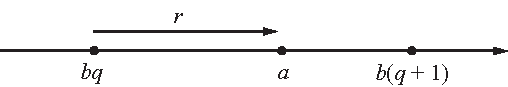
\includegraphics[width=\linewidth]{external/figps-divalgo.pdf}
\end{image}%
\tcblower
\end{figureptx}%
 If \(r\) represents the distance from \(b \cdot q\) to \(a\), then%
\begin{align*}
r \amp = a - b \cdot q,\text{ or }\\
a \amp = b \cdot q + r\text{.}
\end{align*}
From the diagram, also notice that  \(r\)  is less than the distance between \(b \cdot q\) and  \(b\left( {q + 1} \right)\). Algebraically, this distance is%
\begin{align*}
b\left( {q + 1} \right) - b \cdot q \amp = b \cdot q + b - b \cdot q\\
\amp = b\text{.}
\end{align*}
Thus, in the case where  \(a\)  is not a multiple of  \(b\), we get  \(0 \lt  r \lt  b\).%
\item{}We have been implicitly using the fact that an integer cannot be both even and odd. There are several ways to understand this fact, but one way is through the Division Algorithm. When we classify an integer as even or odd, we are doing so on the basis of the remainder (according to the Division Algorithm) when the integer is ``divided'' by 2. If  \(a \in \mathbb{Z}\), then by the Division Algorithm there exist unique integers \(q\) and \(r\) such that%
\begin{equation*}
a = 2q + r\text{ and } 0 \leq r \lt  2\text{.}
\end{equation*}
This means that the remainder, \(r\), can only be zero or one (and not both). When  \(r = 0\), the integer is even, and when \(r = 1\), the integer is odd.%
\end{enumerate}
%
\end{paragraphs}%
\begin{inlineexercise}{Using the Division Algorithm.}{x:exercise:pr_usingdivalgo}%
\begin{enumerate}[font=\bfseries,label=(\alph*),ref=\alph*]
\item{}What are the possible remainders (according to the Division Algorithm) when an integer is%
\begin{enumerate}[font=\bfseries,label=(\roman*),ref=\theenumi.\roman*]
\item{}Divided by 4?%
\space\hyperlink{g:solution:idm826267800-back}{[Solution]}\item{}Divided by 9?%
\space\hyperlink{g:solution:idm826264984-back}{[Solution]}\end{enumerate}
\item{}For each of the following, find the quotient and remainder (guaranteed by the Division Algorithm) and then summarize the results by writing an equation of the form \(a = bq + r\), where \(0 \leq r \lt b\).%
\begin{enumerate}[font=\bfseries,label=(\roman*),ref=\theenumi.\roman*]
\item{}When 17 is divided by 3.%
\space\hyperlink{g:solution:idm826268440-back}{[Solution]}\item{}When \(-17\) is divided by 3.%
\space\hyperlink{g:solution:idm826262040-back}{[Solution]}\item{}When 73 is divded by 7.%
\space\hyperlink{g:solution:idm826255128-back}{[Solution]}\item{}When \(-73\) is divided by 7.%
\space\hyperlink{g:solution:idm826263192-back}{[Solution]}\item{}When 436 is divided by 27.%
\space\hyperlink{g:solution:idm826255640-back}{[Solution]}\item{}When 539 is divided by 110.%
\space\hyperlink{g:solution:idm826261016-back}{[Solution]}\end{enumerate}
\end{enumerate}
\end{inlineexercise}%
\end{subsectionptx}
%
%
\typeout{************************************************}
\typeout{Subsection  Using Cases Determined by the Division Algorithm}
\typeout{************************************************}
%
\begin{subsectionptx}{Using Cases Determined by the Division Algorithm}{}{Using Cases Determined by the Division Algorithm}{}{}{g:subsection:idm826255768}
\index{Division Algorithm!using cases}%
The Division Algorithm  can sometimes be used to construct cases that can be used to prove a statement that is true for all integers. We have done this when we divided the integers into the even integers and the odd integers since even integers have a remainder of 0 when divided by 2 and odd integers have a remainder of 1 when divided by 2.%
\par
Sometimes it is more useful to divide the integer \(a\) by an integer other than 2. For example, if \(a\) is divided by 3, there are three possible remainders: 0, 1, and 2. If \(a\) is divided by 4, there are four possible remainders: 0, 1, 2, and 3. The remainders form the basis for the cases.%
\par
If the hypothesis of a proposition is that ``\(n\) is an integer,'' then we can use the Division Algorithm to claim that there are unique integers \(q\) and \(r\) such that%
\begin{equation*}
n = 3q + r\text{  and  } 0 \leq r \lt  3\text{.}
\end{equation*}
%
\par
We can then divide the proof into the following three cases: (1) \(r = 0\); (2) \(r = 1\); and (3) \(r = 2\). This is done in \hyperref[x:proposition:P_3divides]{Proposition~{\xreffont\ref{x:proposition:P_3divides}}, p.\,\pageref{x:proposition:P_3divides}}.%
\begin{proposition}{}{}{x:proposition:P_3divides}%
If \(n\) is an integer, then 3 divides \(n^3-n\).%
\end{proposition}
\begin{proof}{}{g:proof:idm826510744}
Let \(n\) be an integer. We will show that 3 divides \(n^3-n\) by examining the three cases for the remainder when \(n\) is divided by 3. By the Division Algorithm, there exist unique integers \(q\) and \(r\) such that%
\begin{equation*}
n = 3q + r\text{ , and  } 0 \leq r \lt  3\text{.}
\end{equation*}
%
\par
This means that we can consider the following three cases: (1) \(r = 0\); (2) \(r = 1\); and (3) \(r = 2\).%
\par
In the case where \(r = 0\), we have \(n = 3q\). By substituting this into the expression \(n^3  - n\), we get%
\begin{align*}
n^3 - n \amp = \left( {3q} \right)^3  - \left( {3q} \right)\\
\amp  = 27q^3  - 3q\\
\amp = 3\left( {9q^3  - q} \right)\text{.}
\end{align*}
%
\par
Since \(\left( {9q^3 -q} \right)\) is an integer, the last equation proves that \(3 \mid \left( n^3 - n \right)\).%
\par
In the second case, \(r = 1\) and \(n = 3q + 1\). When we substitute this into \(\left( n^3 - n \right)\), we obtain%
\begin{align*}
n^3 - n \amp = \left( {3q + 1} \right)^3  - \left( {3q + 1} \right)\\
\amp = \left( 27q^3 + 27q^2 +9q + 1\right) - \left( 3q + 1 \right)\\
\amp = 27q^3 + 27q^2 + 6q\\
\amp = 3 \left( 9q^3 + 9q^2 + 2q \right)\text{.}
\end{align*}
%
\par
Since \(\left( {9q^3 +9q^2 + 2q} \right)\) is an integer, the last equation proves that \(3 \mid \left( n^3 - n \right)\).%
\par
The last case is when \(r = 2\). The details for this case are part of \hyperlink{x:exercise:exer_prop3divides}{Exercise~{\xreffont 1}, p.\,\pageref{x:exercise:exer_prop3divides}}. Once this case is completed, we will have proved that 3 divides \(n^3 - n\) in all three cases. Hence, we may conclude that if \(n\) is an integer, then 3 divides \(n^3 - n\).%
\end{proof}
\end{subsectionptx}
%
%
\typeout{************************************************}
\typeout{Subsection  Properties of Congruence}
\typeout{************************************************}
%
\begin{subsectionptx}{Properties of Congruence}{}{Properties of Congruence}{}{}{g:subsection:idm826237992}
\index{congruence}%
Most of the work we have done so far has involved using definitions to help prove results. We will continue to prove some results but we will now prove some theorems about congruence (\hyperref[x:theorem:T_propsofcong]{Theorem~{\xreffont\ref{x:theorem:T_propsofcong}}, p.\,\pageref{x:theorem:T_propsofcong}} and \hyperref[x:theorem:T_modprops]{Theorem~{\xreffont\ref{x:theorem:T_modprops}}, p.\,\pageref{x:theorem:T_modprops}}) that we will then use to help prove other results.%
\par
Let \(n \in \mathbb{N}\). Recall that if \(a\) and \(b\) are integers, then we say that \(a\) is congruent to \(b\) modulo \(n\) provided that \(n\) divides \(a - b\), and we write \(a \equiv b \pmod n\). (See \hyperref[x:section:S_directproof]{Section~{\xreffont\ref{x:section:S_directproof}}, p.\,\pageref{x:section:S_directproof}}.) We are now going to prove some properties of congruence that are direct consequences of the definition. One of these properties was suggested by the work in \hyperref[x:worksheet:PA_congruencereview]{Beginning Activity 2, p.\,\pageref{x:worksheet:PA_congruencereview}} and is \hyperlink{x:li:T_propsofcong1}{Item~{\xreffont 1}, p.\,\pageref{x:li:T_propsofcong1}} of the next theorem.%
\begin{theorem}{Properties of Congruence Modulo.}{}{x:theorem:T_propsofcong}%
Let \(n\) be a natural number and let \(a,
b, c, \text{ and } d\) be integers. If \(a \equiv b \pmod n\) and \(c \equiv d \pmod n\), then%
\begin{enumerate}
\item\label{x:li:T_propsofcong1}{}\hypertarget{x:li:T_propsofcong1}{}\(\left( {a + c} \right) \equiv \left( {b + d} \right) \pmod n\).%
\item\label{x:li:T_propsofcong2}{}\hypertarget{x:li:T_propsofcong2}{}\(ac \equiv bd \pmod n\).%
\item\label{x:li:T_propsofcong3}{}\hypertarget{x:li:T_propsofcong3}{}For each \(m \in \mathbb{N}\), \(a^m \equiv b^m \pmod n\).%
\end{enumerate}
%
\end{theorem}
\begin{proof}{}{g:proof:idm826227240}
We will prove \hyperlink{x:li:T_propsofcong2}{Item~{\xreffont 2}, p.\,\pageref{x:li:T_propsofcong2}} and \hyperlink{x:li:T_propsofcong3}{Item~{\xreffont 3}, p.\,\pageref{x:li:T_propsofcong3}}. The proof of \hyperlink{x:li:T_propsofcong1}{Item~{\xreffont 1}, p.\,\pageref{x:li:T_propsofcong1}} is \hyperref[x:exercise:pr_propsofcong]{Progress Check~{\xreffont\ref{x:exercise:pr_propsofcong}}, p.\,\pageref{x:exercise:pr_propsofcong}}. Let \(n\) be a natural number and let \(a,
b, c, \text{ and } d\) be integers. Assume that \(a \equiv b \pmod n\) and that \(c \equiv d \pmod n\). This means that \(n\) divides \(a-b\) and that \(n\) divides \(c-d\). Hence, there exist integers \(k\) and \(q\) such that \(a-b=nk\) and \(c-d=nq\). We can then write \(a = b + nk\) and \(c = d + nq\) and obtain%
\begin{align*}
ac \amp \left( {b + nk} \right)\left( {d + nq} \right)\\
\amp = bd + bnq + dnk + n^2 kq\\
\amp = bd + n\left( {bq + dk + nkq} \right)\text{.}
\end{align*}
%
\par
By subtracting \(bd\) from both sides of the last equation, we see that%
\begin{equation*}
ac - bd = n\left( {bq + dk + nkq} \right)\text{.}
\end{equation*}
%
\par
Since \(bq + dk + nkq\) is an integer, this proves that \(n \mid \left( {ac - bd} \right)\), and hence we can conclude that \(ac \equiv bd \pmod n\). This completes the proof of \hyperlink{x:li:T_propsofcong2}{Item~{\xreffont 2}, p.\,\pageref{x:li:T_propsofcong2}}.%
\par
\hyperlink{x:li:T_propsofcong2}{Item~{\xreffont 2}, p.\,\pageref{x:li:T_propsofcong2}} basically means that if we have two congruences, we can multiply the corresponding sides of these congruences to obtain another congruence. We have assumed that \(a \equiv b \pmod n\) and so we write this twice as follows:%
\begin{align*}
a \amp \equiv b \pmod n, \text{ and }\\
a \amp \equiv b \pmod n\text{.}
\end{align*}
If we now use the result in \hyperlink{x:li:T_propsofcong2}{Item~{\xreffont 2}, p.\,\pageref{x:li:T_propsofcong2}} and multiply the corresponding sides of these two congruences, we obtain \(a^2 \equiv b^2 \pmod n\). We can then use this congruence and the congruence \(a \equiv b \pmod n\) and the result in \hyperlink{x:li:T_propsofcong2}{Item~{\xreffont 2}, p.\,\pageref{x:li:T_propsofcong2}} to conclude that%
\begin{equation*}
a^2 \cdot a \equiv b^2 \cdot b \pmod n\text{,}
\end{equation*}
or that \(a^3 \equiv b^3 \pmod n\). We can say that we can continue with this process to prove \hyperlink{x:li:T_propsofcong3}{Item~{\xreffont 3}, p.\,\pageref{x:li:T_propsofcong3}}, but this is not considered to be a formal proof of this result. To construct a formal proof for this, we could use a proof by mathematical induction. This will be studied in \hyperref[x:chapter:C_induction]{Chapter~{\xreffont\ref{x:chapter:C_induction}}, p.\,\pageref{x:chapter:C_induction}}. See \hyperlink{x:exercise:exer_sec51-cong}{Exercise~{\xreffont 13}, p.\,\pageref{x:exercise:exer_sec51-cong}} in \hyperref[x:section:S_mathinduction]{Section~{\xreffont\ref{x:section:S_mathinduction}}, p.\,\pageref{x:section:S_mathinduction}}.%
\end{proof}
\begin{inlineexercise}{Proving Item~{\xreffont 1} of Theorem~{\xreffont\ref*{x:theorem:T_propsofcong}}.}{x:exercise:pr_propsofcong}%
Prove \hyperlink{x:li:T_propsofcong1}{Item~{\xreffont 1}, p.\,\pageref{x:li:T_propsofcong1}} of \hyperref[x:theorem:T_propsofcong]{Theorem~{\xreffont\ref{x:theorem:T_propsofcong}}, p.\,\pageref{x:theorem:T_propsofcong}}.%
\space\hyperlink{g:solution:idm826198440-back}{[Solution]}\end{inlineexercise}%
\hyperlink{x:exercise:exer_cong-props}{Exercise~{\xreffont 11}, p.\,\pageref{x:exercise:exer_cong-props}} in \hyperref[x:section:S_directproof]{Section~{\xreffont\ref{x:section:S_directproof}}, p.\,\pageref{x:section:S_directproof}} gave three important properties of congruence modulo \(n\). Because of their importance, these properties are stated and proved in \hyperref[x:theorem:T_modprops]{Theorem~{\xreffont\ref{x:theorem:T_modprops}}, p.\,\pageref{x:theorem:T_modprops}}. Please remember that textbook proofs are usually written in final form of ``reporting the news.'' Before reading these proofs, it might be instructive to first try to construct a know-show~table for each proof.%
\begin{theorem}{Properties of Congruence Modulo \(\boldsymbol{n}\).}{}{x:theorem:T_modprops}%
Let \(n \in \mathbb{N}\), and let \(a\), \(b\), and \(c\) be integers.%
\begin{enumerate}
\item{}\index{congruence!reflexive property}For every integer \(a\), \(a \equiv a \pmod n\).%
\par
This is called the \terminology{reflexive property} of congruence modulo \(n\).%
\item{}If \(a \equiv b \pmod n\), then \(b \equiv a \pmod n\).%
\par
This is called the \terminology{symmetric property} \index{congruence!symmetric property} of congruence modulo \(n\).%
\item{}\index{congruence!transitive property}If \(a \equiv b \pmod n\) and \(b \equiv c \pmod n\), then \(a \equiv c \pmod n\).%
\par
This is called the \emph{transitive property} of congruence modulo \(n\).%
\end{enumerate}
%
\end{theorem}
\begin{proof}{}{g:proof:idm826180776}
We will prove the reflexive property and the transitive property. The proof of the symmetric property is \hyperlink{x:exercise:exer_cong-symm}{Exercise~{\xreffont 3}, p.\,\pageref{x:exercise:exer_cong-symm}}.%
\par
Let \(n \in \mathbb{N}\), and let \(a \in \mathbb{Z}\). We will show that \(a \equiv a \pmod n\). Notice that%
\begin{equation*}
a - a = 0 = n \cdot 0\text{.}
\end{equation*}
%
\par
This proves that \(n\) divides \(\left( {a - a} \right)\) and hence, by the definition of congruence modulo \(n\), we have proven that \(a \equiv a \pmod n\).%
\par
To prove the transitive property, we let \(n \in \mathbb{N}\), and let \(a\), \(b\), and \(c\) be integers. We assume that \(a \equiv b \pmod n\) and that \(b \equiv c \pmod n\). We will use the definition of congruence modulo \(n\) to prove that \(a \equiv c \pmod n\). Since \(a \equiv b \pmod n\) and \(b \equiv c \pmod n\), we know that \(n \mid \left( a-b \right)\) and \(n \mid \left( b-c \right)\). Hence, there exist integers \(k\) and \(q\) such that%
\begin{align*}
a -b \amp = nk\\
b - c \amp = nq\text{.}
\end{align*}
By adding the corresponding sides of these two equations, we obtain%
\begin{equation*}
\left( {a - b} \right) + \left( {b - c} \right) = nk + nq\text{.}
\end{equation*}
If we simplify the left side of the last equation and factor the right side, we get%
\begin{equation*}
a - c = n\left( {k + q} \right)\text{.}
\end{equation*}
By the closure property of the integers, \(\left( {k + q} \right) \in \mathbb{Z}\), and so this equation proves that \(n \mid \left(a-c \right)\) and hence that \(a \equiv c \pmod n\). This completes the proof of the transitive property of congruence modulo \(n\).%
\end{proof}
\end{subsectionptx}
%
%
\typeout{************************************************}
\typeout{Subsection  Using Cases Based on Congruence Modulo \(\boldsymbol{n}\)}
\typeout{************************************************}
%
\begin{subsectionptx}{Using Cases Based on Congruence Modulo \(\boldsymbol{n}\)}{}{Using Cases Based on Congruence Modulo \(\boldsymbol{n}\)}{}{}{g:subsection:idm826166312}
\index{congruence!Division Algorithm}%
\index{Division Algorithm!congruence}%
Notice that the set of all integers that are congruent to 2 modulo 7 is%
\begin{equation*}
\left\{  n \in \Z \mid n \equiv 2 \pmod7 \right\} = 
\left\{ \ldots , - 19, - 12, - 5, 2, 9, 16, 23, \ldots \right\}\text{.}
\end{equation*}
If we divide any integer in this set by 7 and write the result according to the Division Algorithm, we will get a remainder of 2. For example,%
\begin{align*}
2 \amp = 7 \cdot 0 + 2 \amp   -5 \amp = 7 \left( -1 \right) + 2\\
9 \amp = 7 \cdot 1 + 2 \amp   -12 \amp = 7 \left( -2 \right) +2\\
16 \amp = 7 \cdot 2 + 2 \amp   -19 \amp = 7 \left( -3 \right) +2\\
23 \amp = 7 \cdot 3 + 2. \amp    \amp
\end{align*}
Is this a coincidence or is this always true? Let's look at the general case. For this, let \(n\) be a natural number and let \(a \in \mathbb{Z}\). By the Division Algorithm, there exist unique integers \(q\) and \(r\) such that%
\begin{equation*}
a = nq + r\text{ and } 0 \leq r \lt  n\text{.}
\end{equation*}
%
\par
By subtracting \(r\) from both sides of the equation \(a = nq + r\), we obtain%
\begin{equation*}
a - r = nq\text{.}
\end{equation*}
%
\par
But this implies that \(n \mid \left( a - r \right)\) and hence that \(a \equiv r \pmod n\). We have proven the following result.%
\begin{theorem}{}{}{x:theorem:T_congtorem}%
Let \(n \in \mathbb{N}\) and let \(a \in \mathbb{Z}\). If \(a = nq + r\text{ and } 0 \leq r \lt n\) for some integers \(q\) and \(r\), then \(a \equiv r \pmod n\).%
\end{theorem}
This theorem says that an integer is congruent (mod \(n\)) to its remainder when it is divided by \(n\). Since this remainder is unique and since the only possible remainders for division by \(n\) are \(0,1,2, \ldots ,n - 1\), we can state the following result.%
\begin{corollary}{}{}{x:corollary:C_congtorem}%
If \(n \in \mathbb{N}\), then each integer is congruent, modulo \(n\), to precisely one of the integers \(0,1,2, \ldots ,n - 1\). That is, for each integer \(a\), there exists a unique integer \(r\) such that%
\begin{equation*}
a \equiv r \pmod n  \text{ and }   0 \leq r \lt  n\text{.}
\end{equation*}
%
\end{corollary}
\hyperref[x:corollary:C_congtorem]{Corollary~{\xreffont\ref{x:corollary:C_congtorem}}, p.\,\pageref{x:corollary:C_congtorem}} can be used to set up cases for an integer in a proof. If \(n \in \mathbb{N}\) and \(a \in \mathbb{Z}\), then we can consider \(n\) cases for \(a\). The integer \(a\) could be congruent to \(0,1,2, \ldots , \text{ or }  n - 1\) modulo \(n\). For example, if we assume that 5 does not divide an integer \(a\), then we know \(a\) is not congruent to 0 modulo 5, and hence, that \(a\) must be congruent to 1, 2, 3, or 4 modulo 5. We can use these as 4 cases within a proof. For example, suppose we wish to determine the values of \(a^2\) modulo 5 for integers that are not congruent to 0 modulo 5. We begin by squaring some integers that are not congruent to 0 modulo 5. We see that%
\begin{align*}
1^2 \amp = 1 \amp  \text{ and }  \amp  \amp 1 \amp \equiv 1 \pmod 5.\\
3^2 \amp = 9 \amp  \text{ and }  \amp  \amp 9 \amp \equiv 4 \pmod 5.\\
6^2 \amp = 36 \amp  \text{ and }  \amp  \amp 36 \amp \equiv 1 \pmod 5.\\
8^2 \amp = 64 \amp  \text{ and }  \amp  \amp 64 \amp \equiv 4 \pmod 5.\\
9^2 \amp = 81 \amp  \text{ and }  \amp  \amp 81 \amp \equiv 1 \pmod 5\text{.}
\end{align*}
%
\par
These explorations indicate that the following proposition is true and we will now outline a method to prove it.%
\begin{proposition}{}{}{x:proposition:prop_congmod5}%
For each integer \(a\), if \(a \not \equiv 0 \pmod 5\), then \(a^2 \equiv 1 \pmod 5\) or \(a^2 \equiv 4 \pmod 5\).%
\end{proposition}
\begin{proof}{}{g:proof:idm826144936}
We will prove this proposition using cases for \(a\) based on congruence modulo 5. In doing so, we will use the results in \hyperref[x:theorem:T_propsofcong]{Theorem~{\xreffont\ref{x:theorem:T_propsofcong}}, p.\,\pageref{x:theorem:T_propsofcong}} and \hyperref[x:theorem:T_modprops]{Theorem~{\xreffont\ref{x:theorem:T_modprops}}, p.\,\pageref{x:theorem:T_modprops}}. Because the hypothesis is \(a \not \equiv 0 \pmod 5\), we can use four cases, which are: (1) \(a \equiv 1 \pmod 5\), (2) \(a \equiv 2 \pmod 5\), (3) \(a \equiv 3 \pmod 5\), and (4) \(a \equiv 4 \pmod 5\). Following are proofs for the first and fourth cases.%
\par
Case 1. \(\left( a \equiv 1 \pmod 5 \right)\). In this case, we use \hyperref[x:theorem:T_propsofcong]{Theorem~{\xreffont\ref{x:theorem:T_propsofcong}}, p.\,\pageref{x:theorem:T_propsofcong}} to conclude that%
\begin{equation*}
a^2 \equiv 1^2 \pmod 5  \text{ or }   a^2 \equiv 1 \pmod 5\text{.}
\end{equation*}
This proves that if \(a \equiv 1 \pmod 5\), then \(a^2 \equiv 1 \pmod 5\).%
\par
Case 4. \(\left( a \equiv 4 \pmod 5 \right)\). In this case, we use \hyperref[x:theorem:T_propsofcong]{Theorem~{\xreffont\ref{x:theorem:T_propsofcong}}, p.\,\pageref{x:theorem:T_propsofcong}} to conclude that%
\begin{equation*}
a^2 \equiv 1^2 \pmod 5 \text{ or } a^2 \equiv 16 \pmod 5\text{.}
\end{equation*}
%
\par
We also know that \(16 \equiv 1 \pmod 5\). So we have \(a^2 \equiv 16 \pmod 5\) and \(16 \equiv 1 \pmod 5\), and we can now use the transitive property of congruence (\hyperref[x:theorem:T_modprops]{Theorem~{\xreffont\ref{x:theorem:T_modprops}}, p.\,\pageref{x:theorem:T_modprops}}) to conclude that \(a^2 \equiv 1 \pmod 5\). This proves that if \(a \equiv 4 \pmod 5\), then \(a^2 \equiv 1 \pmod 5\).%
\end{proof}
\begin{inlineexercise}{Using Properties of Congruence.}{x:exercise:prog_propertiesofcong}%
Complete a proof of \hyperref[x:proposition:prop_congmod5]{Proposition~{\xreffont\ref{x:proposition:prop_congmod5}}, p.\,\pageref{x:proposition:prop_congmod5}} by completing proofs for the other two cases.%
\par
Note: It is possible to prove \hyperref[x:proposition:prop_congmod5]{Proposition~{\xreffont\ref{x:proposition:prop_congmod5}}, p.\,\pageref{x:proposition:prop_congmod5}} using only the definition of congruence instead of using the properties that we have proved about congruence. However, such a proof would involve a good deal of algebra. One of the advantages of using the properties is that it avoids the use of complicated algebra in which it is easy to make mistakes.%
\space\hyperlink{g:solution:idm826128808-back}{[Solution]}\end{inlineexercise}%
In the proof of \hyperref[x:proposition:prop_congmod5]{Proposition~{\xreffont\ref{x:proposition:prop_congmod5}}, p.\,\pageref{x:proposition:prop_congmod5}}, we used four cases. Sometimes it may seem a bit overwhelming when confronted with a proof that requires several cases. For example, if we want to prove something about some integers modulo 6, we may have to use six cases. However, there are sometimes additional assumptions (or conclusions) that can help reduce the number of cases that must be considered. This will be illustrated in the next progress check.%
\begin{inlineexercise}{Using Cases Modulo 6.}{x:exercise:prog_casesmod6}%
Suppose we want to determine the possible values for \(a^2\) modulo 6 for odd integers that are not multiples of 3. Before beginning to use congruence arithmetic (as in the proof of \hyperref[x:proposition:prop_congmod5]{Proposition~{\xreffont\ref{x:proposition:prop_congmod5}}, p.\,\pageref{x:proposition:prop_congmod5}}) in each of the possible six cases, we can show that some of the cases are not possible under these assumptions. (In some sense, we use a short proof by contradiction for these cases.) So assume that \(a\) is an odd integer. Then:%
\begin{itemize}[label=\textbullet]
\item{}If \(a \equiv 0 \pmod 6\), then there exists an integer \(k\) such that \(a = 6k\). But then \(a = 2(3k)\) and hence, \(a\) is even. Since we assumed that \(a\) is odd, this case is not possible.%
\item{}If \(a \equiv 2 \pmod 6\), then there exists an integer \(k\) such that \(a = 6k + 2\). But then \(a = 2(3k + 1)\) and hence, \(a\) is even. Since we assumed that \(a\) is odd, this case is not possible.%
\end{itemize}
%
\begin{enumerate}[font=\bfseries,label=(\alph*),ref=\alph*]
\item{}Prove that if \(a\) is an odd integer, then \(a\) cannot be congruent to 4 modulo 6.%
\item{}Prove that if \(a\) is an integer and 3 does not divide \(a\), then \(a\) cannot be congruent to 3 modulo 6.%
\item{}So if \(a\) is an odd integer that is not a multiple of 3, then \(a\) must be congruent to 1 or 5 modulo 6. Use these two cases to prove the following proposition: \begin{proposition}{}{}{x:proposition:prop_congmod6}%
For each integer \(a\), if \(a\) is an odd integer that is not multiple of 3, then \(a^2 \equiv 1 \pmod 6\).%
\end{proposition}
%
\end{enumerate}
\end{inlineexercise}%
\end{subsectionptx}
%
%
\typeout{************************************************}
\typeout{Exercises  Exercises}
\typeout{************************************************}
%
\begin{exercises-subsection}{Exercises}{}{Exercises}{}{}{g:exercises:idm826104872}
\begin{divisionexercise}{1}{}{}{x:exercise:exer_prop3divides}%
Complete the details for the proof of Case 3 of \hyperref[x:proposition:P_3divides]{Proposition~{\xreffont\ref{x:proposition:P_3divides}}, p.\,\pageref{x:proposition:P_3divides}}.%
\end{divisionexercise}%
\begin{divisionexercise}{2}{}{}{g:exercise:idm826102184}%
Complete the following.%
\begin{enumerate}[font=\bfseries,label=(\alph*),ref=\alph*]
\item\label{x:task:exer-cases3-a}Use cases based on congruence modulo 3 and properties of congruence to prove that for each integer \(n\), \(n^3 \equiv n \pmod 3\).%
\space\hyperlink{g:answer:idm826107048-back}{[Answer]}\item{}Explain why the result in \hyperref[x:task:exer-cases3-a]{Task~{\xreffont 2}.{\xreffont\ref{x:task:exer-cases3-a}}, p.\,\pageref{x:task:exer-cases3-a}} proves that for each integer \(n\), 3 divides \(\left(n^3 - n \right)\). Compare this to the proof of the same result in \hyperref[x:proposition:P_3divides]{Proposition~{\xreffont\ref{x:proposition:P_3divides}}, p.\,\pageref{x:proposition:P_3divides}}.%
\space\hyperlink{g:answer:idm826097192-back}{[Answer]}\end{enumerate}
\end{divisionexercise}%
\begin{divisionexercise}{3}{}{}{x:exercise:exer_cong-symm}%
Prove the symmetric property of congruence stated in \hyperref[x:theorem:T_modprops]{Theorem~{\xreffont\ref{x:theorem:T_modprops}}, p.\,\pageref{x:theorem:T_modprops}}.%
\space\hyperlink{g:answer:idm826098088-back}{[Answer]}\end{divisionexercise}%
\begin{divisionexercise}{4}{}{}{x:exercise:exer_sec35-a2mod3}%
Consider the following proposition: For each integer \(a\), if 3 divides \(a^2\), then 3 divides \(a\).%
\begin{enumerate}[font=\bfseries,label=(\alph*),ref=\alph*]
\item{}Write the contrapositive of this proposition.%
\space\hyperlink{g:answer:idm826087080-back}{[Answer]}\item{}Prove the proposition by proving its contrapositive.%
\space\hyperlink{g:hint:idm826088104-back}{[Hint]}\space\hyperlink{g:answer:idm826079144-back}{[Answer]}\end{enumerate}
\end{divisionexercise}%
\begin{divisionexercise}{5}{}{}{x:exercise:exer_sec34-4}%
Complete the following.%
\begin{enumerate}[font=\bfseries,label=(\alph*),ref=\alph*]
\item{}Let \(n \in \mathbb{N}\) and let \(a \in \mathbb{Z}\). Explain why \(n\) divides \(a\) if and only if \(a \equiv 0 \pmod n\).%
\space\hyperlink{g:answer:idm826080936-back}{[Answer]}\item\label{x:task:exer_sec34-4b}Let \(a \in \mathbb{Z}\). Explain why if \(a \not \equiv 0 \pmod 3\), then \(a \equiv 1\pmod 3\) or \(a \equiv 2 \pmod 3\).%
\space\hyperlink{g:answer:idm826070568-back}{[Answer]}\item\label{x:task:exer_sec34-4c}Is the following proposition true or false? Justify your conclusion. \begin{quote}%
For each \(a \in \mathbb{Z}\), if \(a \not \equiv 0 \pmod 3\), then \(a^2 \equiv 1 \pmod 3\).\end{quote}
%
\space\hyperlink{g:answer:idm826070440-back}{[Answer]}\end{enumerate}
\end{divisionexercise}%
\begin{divisionexercise}{6}{}{}{x:exercise:exer_congto3}%
Prove the following proposition by proving its contrapositive. \begin{quote}%
For all integers \(a\) and \(b\), if \(ab \equiv 0 \pmod 3\), then \(a \equiv 0 \pmod 3\) or \(b \equiv 0 \pmod 3\).\end{quote}
%
\space\hyperlink{g:hint:idm826061864-back}{[Hint]}\space\hyperlink{g:answer:idm826058920-back}{[Answer]}\end{divisionexercise}%
\begin{divisionexercise}{7}{}{}{x:exercise:exer_3divprod}%
Complete the following.%
\begin{enumerate}[font=\bfseries,label=(\alph*),ref=\alph*]
\item\label{x:task:exer_3divproda}Explain why the following proposition is equivalent to the proposition in \hyperlink{x:exercise:exer_congto3}{Exercise~{\xreffont 6}, p.\,\pageref{x:exercise:exer_congto3}}. \begin{quote}%
For all integers \(a\) and \(b\), if \(3 \mid ab\) , then \(3 \mid a\) or \(3 \mid b\).\end{quote}
%
\space\hyperlink{g:answer:idm826042920-back}{[Answer]}\item{}Prove that for each integer \(a\), if 3 divides \(a^2\), then 3 divides \(a\).%
\space\hyperlink{g:answer:idm826040232-back}{[Answer]}\end{enumerate}
\end{divisionexercise}%
\begin{divisionexercise}{8}{}{}{x:exercise:exer_sqrt3}%
Complete the following.%
\begin{enumerate}[font=\bfseries,label=(\alph*),ref=\alph*]
\item{}Prove that the real number \(\sqrt{3}\) is an irrational number. That is, prove that \begin{quote}%
If \(r\) is a positive real number such that \(r^2 = 3\), then \(r\) is irrational.\end{quote}
%
\space\hyperlink{g:hint:idm826036648-back}{[Hint]}\item{}Prove that the real number \(\sqrt{12}\) is an irrational number.%
\end{enumerate}
\end{divisionexercise}%
\begin{divisionexercise}{9}{}{}{x:exercise:exer_notperfectsquare}%
Prove that for each natural number \(n\), \(\sqrt{3n + 2}\) is not a natural number.%
\space\hyperlink{g:hint:idm826031144-back}{[Hint]}\end{divisionexercise}%
\begin{divisionexercise}{10}{}{}{x:exercise:exer_sec34-2}%
Extending the idea in \hyperlink{x:exercise:exer_consecutive}{Exercise~{\xreffont 1}, p.\,\pageref{x:exercise:exer_consecutive}} of \hyperref[x:section:S_cases]{Section~{\xreffont\ref{x:section:S_cases}}, p.\,\pageref{x:section:S_cases}}, we can represent three consecutive integers as \(m\), \(m + 1\), and \(m + 2\), where \(m\) is an integer.%
\begin{enumerate}[font=\bfseries,label=(\alph*),ref=\alph*]
\item{}Explain why we can also represent three consecutive integers as \(k - 1\), \(k\), and \(k + 1\), where \(k\) is an integer.%
\item{}Explain why \hyperref[x:proposition:P_3divides]{Proposition~{\xreffont\ref{x:proposition:P_3divides}}, p.\,\pageref{x:proposition:P_3divides}} proves that the product of any three consecutive integers is divisible by 3.%
\space\hyperlink{g:hint:idm826033448-back}{[Hint]}\item{}Prove that the product of three consecutive integers is divisible by 6.%
\space\hyperlink{g:hint:idm826031400-back}{[Hint]}\end{enumerate}
\end{divisionexercise}%
\begin{divisionexercise}{11}{}{}{x:exercise:exer_squaremod5}%
Complete the following.%
\begin{enumerate}[font=\bfseries,label=(\alph*),ref=\alph*]
\item{}Use the result in \hyperref[x:proposition:prop_congmod5]{Proposition~{\xreffont\ref{x:proposition:prop_congmod5}}, p.\,\pageref{x:proposition:prop_congmod5}} to help prove that the integer \(m = 5,344,580,232,468,953,153\) is not a perfect square. Recall that an integer \(n\) is a perfect square provided that there exists an integer \(k\) such that \(n = k^2\).%
\space\hyperlink{g:hint:idm826021416-back}{[Hint]}\item{}Is the integer \(n = 782,456,231,189,002,288, 438\) a perfect square? Justify your conclusion.%
\end{enumerate}
\end{divisionexercise}%
\begin{divisionexercise}{12}{}{}{x:exercise:exer_sqrt5-irrational}%
Complete the following.%
\begin{enumerate}[font=\bfseries,label=(\alph*),ref=\alph*]
\item{}Use the result in \hyperref[x:proposition:prop_congmod5]{Proposition~{\xreffont\ref{x:proposition:prop_congmod5}}, p.\,\pageref{x:proposition:prop_congmod5}} to help prove that for each integer \(a\), if 5 divides \(a^2\), then 5 divides \(a\).%
\item{}Prove that the real number \(\sqrt{5}\) is an irrational number.%
\end{enumerate}
\end{divisionexercise}%
\begin{divisionexercise}{13}{}{}{g:exercise:idm826017960}%
Prove the following.%
\begin{enumerate}[font=\bfseries,label=(\alph*),ref=\alph*]
\item{}For each integer \(a\), if \(a \not \equiv 0 \pmod 7\), then \(a^2 \not \equiv 0 \pmod 7\).%
\item{}For each integer \(a\), if 7 divides \(a^2\), then 7 divides \(a\).%
\item{}The real number \(\sqrt{7}\) is an irrational number.%
\end{enumerate}
\end{divisionexercise}%
\begin{divisionexercise}{14}{}{}{x:exercise:exer_remainderbycong}%
Complete the following.%
\begin{enumerate}[font=\bfseries,label=(\alph*),ref=\alph*]
\item{}If an integer has a remainder of 6 when it is divided by 7, is it possible to determine the remainder of the square of that integer when it is divided by 7? If so, determine the remainder and prove that your answer is correct.%
\item{}If an integer has a remainder of 11 when it is divided by 12, is it possible to determine the remainder of the square of that integer when it is divided by 12? If so, determine the remainder and prove that your answer is correct.%
\item{}Let \(n\) be a natural number greater than 2. If an integer has a remainder of \(n - 1\) when it is divided by \(n\), is it possible to determine the remainder of the square of that integer when it is divided by \(n\)? If so, determine the remainder and prove that your answer is correct.%
\end{enumerate}
\end{divisionexercise}%
\begin{divisionexercise}{15}{}{}{g:exercise:idm826012968}%
Let \(n\) be a natural number greater than 4 and let \(a\) be an integer that has a remainder of \(n - 2\) when it is divided by \(n\). Make whatever conclusions you can about the remainder of \(a^2\) when it is divided by \(n\). Justify all conclusions.%
\end{divisionexercise}%
\begin{divisionexercise}{16}{}{}{g:exercise:idm826006184}%
Is the following proposition true or false? Justify your conclusion with a proof or a counterexample. \begin{quote}%
For each natural number \(n\), if 3 does not divide \(\left( n^2 + 2 \right)\), then \(n\) is not a prime number or \(n=3\).\end{quote}
%
\end{divisionexercise}%
\begin{divisionexercise}{17}{}{}{x:exercise:exer_sec34-new9}%
Complete the following.%
\begin{enumerate}[font=\bfseries,label=(\alph*),ref=\alph*]
\item{}Is the following proposition true or false? Justify your conclusion with a counterexample or a proof. \begin{quote}%
For each integer \(n\), if \(n\) is odd, then \(n^2 \equiv 1 \pmod 8\).\end{quote}
%
\item{}Compare this proposition to the proposition in \hyperlink{x:exercise:exer_sec34-nsquared}{Exercise~{\xreffont 7}, p.\,\pageref{x:exercise:exer_sec34-nsquared}} from \hyperref[x:section:S_cases]{Section~{\xreffont\ref{x:section:S_cases}}, p.\,\pageref{x:section:S_cases}}. Are these two propositions equivalent? Explain.%
\item{}Is the following proposition true or false? Justify your conclusion with a counterexample or a proof. \begin{quote}%
For each integer \(n\), if \(n\) is odd and \(n\) is not a multiple of 3, then \(n^2 \equiv 1 \pmod {24}\).\end{quote}
%
\end{enumerate}
\end{divisionexercise}%
\begin{divisionexercise}{18}{}{}{g:exercise:idm825997992}%
Prove the following proposition: \begin{quote}%
For all integers \(a\) and \(b\), if 3 divides \(\left( a^2 + b^2 \right)\), then 3 divides \(a\) and 3 divides \(b\).\end{quote}
%
\end{divisionexercise}%
\begin{divisionexercise}{19}{}{}{x:exercise:exer_case-ind}%
Is the following proposition true or false? Justify your conclusion with a counterexample or a proof. \begin{quote}%
For each integer \(a\), 3 divides \(a^3 + 23a\).\end{quote}
%
\end{divisionexercise}%
\begin{divisionexercise}{20}{}{}{x:exercise:exer_falsecongruence}%
Are the following statements true or false? Either prove the statement is true or provide a counterexample to show it is false.%
\begin{enumerate}[font=\bfseries,label=(\alph*),ref=\alph*]
\item{}For all integers \(a\) and \(b\), if \(a \cdot b \equiv 0 \pmod 6\), then \(a \equiv 0 \pmod 6\) or \(b \equiv 0 \pmod 6\).%
\item{}For all integers \(a\) and \(b\), if \(a \cdot b \equiv 0 \pmod 8\), then \(a \equiv 0 \pmod 8\) or \(b \equiv 0 \pmod 8\).%
\item{}For all integers \(a\) and \(b\), if \(a \cdot b \equiv 1 \pmod 6\), then \(a \equiv 1 \pmod 6\) or \(b \equiv 1 \pmod 6\).%
\item{}For all integers \(a\) and \(b\), if \(ab \equiv 7 \pmod 12\), then either \(a \equiv 1 \pmod 12\) or \(a \equiv 7 \pmod 12\).%
\end{enumerate}
\end{divisionexercise}%
\begin{divisionexercise}{21}{}{}{g:exercise:idm825984168}%
Complete the following.%
\begin{enumerate}[font=\bfseries,label=(\alph*),ref=\alph*]
\item{}Determine several pairs of integers \(a\) and \(b\) such that \(a \equiv b \pmod 5\). For each such pair, calculate \(4a + b\), \(3a + 2b\), and \(7a + 3b\). Are each of the resulting integers congruent to 0 modulo 5?%
\item{}Prove or disprove the following proposition: \begin{quote}%
Let \(m\) and \(n\) be integers such that \((m + n) \equiv 0 \pmod 5\) and let \(a, b \in \Z\). If \(a \equiv b \pmod 5\), then \((ma +nb) \equiv 0 \pmod 5\).\end{quote}
%
\end{enumerate}
\end{divisionexercise}%
\begin{divisionexercise}{22}{Evaluation of Proofs.}{}{g:exercise:idm825680056}%
See the instructions for \hyperlink{x:exercise:exer_proofeval}{Exercise~{\xreffont 19}, p.\,\pageref{x:exercise:exer_proofeval}} from \hyperref[x:section:S_directproof]{Section~{\xreffont\ref{x:section:S_directproof}}, p.\,\pageref{x:section:S_directproof}}.%
\begin{enumerate}[font=\bfseries,label=(\alph*),ref=\alph*]
\item{}%
\begin{descriptionlist}
\begin{dlinarrow}{Proposition}{g:li:idm825674168}%
For all integers \(a\) and \(b\), if \((a + 2b) \equiv 0 \pmod 3\), then \((2a + b) \equiv 0 \pmod 3\).%
\end{dlinarrow}%
\begin{dlinarrow}{Proof}{g:li:idm825680568}%
We assume \(a, b \in \Z\) and \((a + 2b) \equiv 0 \pmod 3\). This means that 3 divides \(a + 2b\) and, hence, there exists an integer \(m\) such that \(a + 2b = 3m\). Hence, \(a = 3m - 2b\). For \((2a + b) \equiv 0 \pmod 3\), there exists an integer \(x\) such that \(2a + b = 3x\). Hence,%
\begin{align*}
2(3m - 2b) + b \amp = 3x\\
6m - 3b \amp = 3x\\
3(2m - b) \amp = 3x\\
2m - b \amp = x\text{.}
\end{align*}
%
\par
Since \((2m - b)\) is an integer, this proves that 3 divides \((2a + b)\) and hence, \((2a + b) \equiv 0 \pmod 3\).%
\end{dlinarrow}%
\end{descriptionlist}
%
\item{}%
\begin{descriptionlist}
\begin{dlinarrow}{Proposition}{g:li:idm825669176}%
For each integer \(m\), 5 divides \(\left(m^5 - m \right)\).%
\end{dlinarrow}%
\begin{dlinarrow}{Proof}{g:li:idm825662776}%
Let \(m \in \Z\). We will prove that 5 divides \(\left(m^5 - m \right)\) by proving that \(\left(m^5 - m \right) \equiv 0 \pmod 5\). We will use cases.%
\par
For the first case, if \(m \equiv 0 \pmod 5\), then \(m^5 \equiv 0 \pmod 5\) and, hence, \(\left(m^5 - m \right) \equiv 0 \pmod 5\).%
\par
For the second case, if \(m \equiv 1 \pmod 5\), then \(m^5 \equiv 1 \pmod 5\) and, hence, \(\left(m^5 - m \right) \equiv (1 - 1) \pmod 5\), which means that \(\left(m^5 - m \right) \equiv 0 \pmod 5\).%
\par
For the third case, if \(m \equiv 2 \pmod 5\), then \(m^5 \equiv 32 \pmod 5\) and, hence, \(\left(m^5 - m \right) \equiv (32 - 2) \pmod 5\), which means that \(\left(m^5 - m \right) \equiv 0 \pmod 5\).%
\end{dlinarrow}%
\end{descriptionlist}
%
\end{enumerate}
\end{divisionexercise}%
\begin{activity}{Using a Contradiction to Prove a Case Is Not Possible.}{x:activity:exer_sec34-9}%
Explore the statements in \hyperref[x:task:exer_sec35-9a]{Task~{\xreffont\ref{x:activity:exer_sec34-9}}.{\xreffont\ref{x:task:exer_sec35-9a}}, p.\,\pageref{x:task:exer_sec35-9a}} and \hyperref[x:task:exer_sec35-9b]{Task~{\xreffont\ref{x:activity:exer_sec34-9}}.{\xreffont\ref{x:task:exer_sec35-9b}}, p.\,\pageref{x:task:exer_sec35-9b}} by considering several examples where the hypothesis is true.%
\begin{enumerate}[font=\bfseries,label=(\alph*),ref=\alph*]
\item\label{x:task:exer_sec35-9a}If an integer \(a\) is divisible by both 4 and 6, then it divisible by 24.%
\item\label{x:task:exer_sec35-9b}If an integer \(a\) is divisible by both 2 and 3, then it divisible by 6.%
\item{}What can you conclude from the examples in \hyperref[x:task:exer_sec35-9a]{Task~{\xreffont\ref{x:activity:exer_sec34-9}}.{\xreffont\ref{x:task:exer_sec35-9a}}, p.\,\pageref{x:task:exer_sec35-9a}}?%
\item{}What can you conclude from the examples in \hyperref[x:task:exer_sec35-9b]{Task~{\xreffont\ref{x:activity:exer_sec34-9}}.{\xreffont\ref{x:task:exer_sec35-9b}}, p.\,\pageref{x:task:exer_sec35-9b}}?%
\end{enumerate}
The proof of the following proposition based on \hyperref[x:task:exer_sec35-9b]{Task~{\xreffont\ref{x:activity:exer_sec34-9}}.{\xreffont\ref{x:task:exer_sec35-9b}}, p.\,\pageref{x:task:exer_sec35-9b}} uses cases. In this proof, however, we use cases and a proof by contradiction to prove that a certain integer cannot be odd.  Hence, it must be even.  Complete the proof of the proposition.%
\begin{descriptionlist}
\begin{dlinarrow}{Proposition}{g:li:idm825651128}%
Let \(a \in \mathbb{Z}\). If 2 divides \(a\) and 3 divides \(a\), then 6 divides \(a\).%
\end{dlinarrow}%
\begin{dlinarrow}{Proof}{g:li:idm825640888}%
Let \(a \in \mathbb{Z}\) and assume that 2 divides \(a\) and 3 divides \(a\). We will prove that 6 divides \(a\). Since 3 divides \(a\), there exists an integer \(n\) such that%
\begin{equation*}
a = 3n\text{.}
\end{equation*}
The integer \(n\) is either even or it is odd. We will show that it must be even by obtaining a contradiction if it assumed to be odd. So, assume that \(n\) is odd. (Now complete the proof.)%
\end{dlinarrow}%
\end{descriptionlist}
%
\end{activity}%
\begin{activity}{The Last Two Digits of a Large Integer.}{g:activity:idm825641528}%
Notice that \(7,381,272 \equiv 72 \pmod 100\) since \(7,381,272 - 72 = 7,381,200\), which is divisible by 100. In general, if we start with an integer whose decimal representation has more than two digits and subtract the integer formed by the last two digits, the result will be an integer whose last two digits are 00. This result will be divisible by 100. Hence, any integer with more than 2 digits is congruent modulo 100 to the integer formed by its last two digits.%
\begin{enumerate}[font=\bfseries,label=(\alph*),ref=\alph*]
\item\label{x:task:A_lasttwo1}Start by squaring both sides of the congruence \(3^4 \equiv 81 \pmod {100}\) to prove that \(3^8 \equiv 61 \pmod {100}\) and then prove that \(3^{16} \equiv 21 \pmod {100}\). What does this tell you about the last two digits in the decimal representation of \(3^{16}\)?%
\item{}Use the two congruences in \hyperref[x:task:A_lasttwo1]{Task~{\xreffont\ref{g:activity:idm825641528}}.{\xreffont\ref{x:task:A_lasttwo1}}, p.\,\pageref{x:task:A_lasttwo1}} and laws of exponents to determine \(r\) where \(3^{20} \equiv r \pmod {100}\) and \(r \in \mathbb{Z}\) with \(0 \leq r \lt 100\) . What does this tell you about the last two digits in the decimal representation of \(3^{20}\)?%
\item{}Determine the last two digits in the decimal representation of \(3^{400}\).%
\item{}Determine the last two digits in the decimal representation of \(4^{804}\).%
\space\hyperlink{g:hint:idm825640120-back}{[Hint]}\par\smallskip%
\noindent\textbf{\blocktitlefont Hint}.\label{g:hint:idm825640120}{}\hypertarget{g:hint:idm825640120}{}\quad{}One way is to determine the ``mod 100 values'' for \(4^2\), \(4^4\), \(4^8\), \(4^{16}\), \(4^{32}\), \(4^{64}\),~and so on. Then use these values and laws of exponents to determine \(r\), where \(4^{804} \equiv r \pmod {100}\) and \(r \in \mathbb{Z}\) with \(0 \leq r \lt 100\).%
\item{}Determine the last two digits in the decimal representation of \(3^{3356}\).%
\item{}Determine the last two digits in the decimal representation of \(7^{403}\).%
\end{enumerate}
\end{activity}%
\end{exercises-subsection}
\end{sectionptx}
%
%
\typeout{************************************************}
\typeout{Section 3.6 Review of Proof Methods}
\typeout{************************************************}
%
\begin{sectionptx}{Review of Proof Methods}{}{Review of Proof Methods}{}{}{x:section:S_reviewproofs}
\begin{introduction}{}%
This section is different from others in the text. It is meant primarily as a review of the proof methods studied in \hyperref[x:chapter:C_proofs]{Chapter~{\xreffont\ref{x:chapter:C_proofs}}, p.\,\pageref{x:chapter:C_proofs}}. So the first part of the section will be a description of some of the main proof techniques introduced in \hyperref[x:chapter:C_proofs]{Chapter~{\xreffont\ref{x:chapter:C_proofs}}, p.\,\pageref{x:chapter:C_proofs}}. The most important part of this section is the set of exercises since these exercises will provide an opportunity to use the proof techniques that we have studied so far.%
\par
We will now give descriptions of three of the most common methods used to prove a conditional statement.%
\end{introduction}%
%
%
\typeout{************************************************}
\typeout{Subsection  Direct Proof of a Conditional Statement \(\boldsymbol{\left( P \to Q \right)}\)}
\typeout{************************************************}
%
\begin{subsectionptx}{Direct Proof of a Conditional Statement \(\boldsymbol{\left( P \to Q \right)}\)}{}{Direct Proof of a Conditional Statement \(\boldsymbol{\left( P \to Q \right)}\)}{}{}{g:subsection:idm825631416}
\index{direct proof}%
\index{proof!direct}%
%
\begin{itemize}[label=\textbullet]
\item{}\lititle{When is it indicated?}\par%
This type of proof is often used when the hypothesis and the conclusion are both stated in a ``positive'' manner. That is, no negations are evident in the hypothesis and conclusion.%
\item{}\lititle{Description of the process.}\par%
Assume that \(P\) is true and use this to conclude that \(Q\) is true. That is, we use the forward-backward method and work forward from \(P\) and backward from \(Q\).%
\item{}\lititle{Why the process makes sense.}\par%
We know that the conditional statement \(P \to Q\) is automatically true when the hypothesis is false. Therefore, because our goal is to prove that \(P \to Q\) is true, there is nothing to do in the case that \(P\) is false. Consequently, we may assume that \(P\) is true. Then, in order for \(P \to Q\) to be true, the conclusion \(Q\) must also be true. (When \(P\) is true, but \(Q\) is false, \(P \to Q\) is false.) Thus, we must use our assumption that \(P\) is true to show that \(Q\) is also true.%
\end{itemize}
%
\end{subsectionptx}
%
%
\typeout{************************************************}
\typeout{Subsection  Proof of a Conditional Statement \(\boldsymbol{\left( P \to Q \right)}\) Using the Contrapositive}
\typeout{************************************************}
%
\begin{subsectionptx}{Proof of a Conditional Statement \(\boldsymbol{\left( P \to Q \right)}\) Using the Contrapositive}{}{Proof of a Conditional Statement \(\boldsymbol{\left( P \to Q \right)}\) Using the Contrapositive}{}{}{g:subsection:idm825614264}
\index{contrapositive}%
\index{proof!contrapositive}%
%
\begin{itemize}[label=\textbullet]
\item{}\lititle{When is it indicated?}\par%
This type of proof is often used when both the hypothesis and the conclusion are stated in the form of negations. This often works well if the conclusion contains the operator ``or''; that is, if the conclusion is in the form of a disjunction. In this case, the negation will be a conjunction.%
\item{}\lititle{Description of the process.}\par%
We prove the logically equivalent statement \(\mynot Q \to \mynot P\). The forward-backward method is used to prove \(\mynot Q \to \mynot P\). That is, we work forward from \(\mynot Q\) and backward from \(\mynot P\).%
\item{}\lititle{Why the process makes sense.}\par%
When we prove \(\mynot Q \to \mynot P\), we are also proving \(P \to Q\) because these two statements are logically equivalent. When we prove the contrapositive of \(P \to Q\), we are doing a direct proof of \(\mynot Q \to \mynot P\). So we assume \(\mynot Q\) because, when doing a direct proof, we assume the hypothesis, and \(\mynot Q\) is the hypothesis of the contrapositive. We must show \(\mynot P\) because it is the conclusion of the contrapositive.%
\end{itemize}
%
\end{subsectionptx}
%
%
\typeout{************************************************}
\typeout{Subsection  Proof of \(\boldsymbol{\left( P \to Q \right)}\) Using a Proof by Contradiction}
\typeout{************************************************}
%
\begin{subsectionptx}{Proof of \(\boldsymbol{\left( P \to Q \right)}\) Using a Proof by Contradiction}{}{Proof of \(\boldsymbol{\left( P \to Q \right)}\) Using a Proof by Contradiction}{}{}{g:subsection:idm825603896}
\index{contradiction}%
\index{proof!by contradiction}%
%
\begin{itemize}[label=\textbullet]
\item{}\lititle{When is it indicated?}\par%
This type of proof is often used when the conclusion is stated in the form of a negation, but the hypothesis is not. This often works well if the conclusion contains the operator ``or''; that is, if the conclusion is in the form of a disjunction. In this case, the negation will be a conjunction.%
\item{}\lititle{Description of the process.}\par%
Assume \(P\) and \(\mynot Q\) and work forward from these two assumptions until a contradiction is obtained.%
\item{}\lititle{Why the process makes sense.}\par%
The statement \(P \to Q\) is either true or false. In a proof by contradiction, we show that it is true by eliminating the only other possibility (that it is false). We show that \(P \to Q\) cannot be false by assuming it is false and reaching a contradiction. Since we assume that \(P \to Q\) is false, and the only way for a conditional statement to be false is for its hypothesis to be true and its conclusion to be false, we assume that \(P\) is true and that \(Q\) is false (or, equivalently, that \(\mynot Q\) is true). When we reach a contradiction, we know that our original assumption that \(P \to Q\) is false is incorrect. Hence, \(P \to Q\) cannot be false, and so it must be true.%
\end{itemize}
%
\end{subsectionptx}
%
%
\typeout{************************************************}
\typeout{Subsection  Other Methods of Proof}
\typeout{************************************************}
%
\begin{subsectionptx}{Other Methods of Proof}{}{Other Methods of Proof}{}{}{g:subsection:idm825592120}
\begin{introduction}{}%
The methods of proof that were just described are three of the most common types of proof. However, we have seen other methods of proof and these are described below.%
\end{introduction}%
%
%
\typeout{************************************************}
\typeout{Subsubsection  Proofs that Use a Logical Equivalency}
\typeout{************************************************}
%
\begin{subsubsectionptx}{Proofs that Use a Logical Equivalency}{}{Proofs that Use a Logical Equivalency}{}{}{g:subsubsection:idm825593528}
As was indicated in \hyperref[x:section:S_moremethods]{Section~{\xreffont\ref{x:section:S_moremethods}}, p.\,\pageref{x:section:S_moremethods}}, we can sometimes use a logical equivalency to help prove a statement. For example, in order to prove a statement of the form%
\begin{equation}
P \to \left( {Q \vee R} \right)\text{,}\label{x:men:eq_reviewproofs1}
\end{equation}
it is sometimes possible to use the logical equivalency%
\begin{equation*}
\left[ {P \to \left( {Q \vee R} \right)} \right] \equiv \left[ {\left( {P \wedge 
\mynot  Q} \right) \to R} \right]\text{.}
\end{equation*}
We would then prove the statement%
\begin{equation}
\left( {P \wedge \mynot Q} \right) \to R\text{.}\label{x:men:eq_reviewproofs2}
\end{equation}
Most often, this would use a direct proof for statement \hyperref[x:men:eq_reviewproofs2]{({\xreffont\ref{x:men:eq_reviewproofs2}})} but other methods could also be used. Because of the logical equivalency, by proving statement \hyperref[x:men:eq_reviewproofs2]{({\xreffont\ref{x:men:eq_reviewproofs2}})}, we have also proven the statement \hyperref[x:men:eq_reviewproofs1]{({\xreffont\ref{x:men:eq_reviewproofs1}})}.%
\end{subsubsectionptx}
%
%
\typeout{************************************************}
\typeout{Subsubsection  Proofs that Use Cases}
\typeout{************************************************}
%
\begin{subsubsectionptx}{Proofs that Use Cases}{}{Proofs that Use Cases}{}{}{g:subsubsection:idm825584312}
\index{cases, proof using}%
\index{proof!using cases}%
When we are trying to prove a proposition or a theorem, we often run into the problem that there does not seem to be enough information to proceed. In this situation, we will sometimes use cases to provide additional assumptions for the forward process of the proof. When this is done, the original proposition is divided into a number of separate cases that are proven independently of each other. The cases must be chosen so that they exhaust all possibilities for the hypothesis of the original proposition. This method of case analysis is justified by the logical equivalency%
\begin{equation*}
\left( {P \vee Q} \right) \to R \equiv \left( {P \to R} \right) \wedge 
\left( {Q \to R} \right)\text{,}
\end{equation*}
which was established in \hyperref[x:worksheet:PA_logicalequiv]{Beginning Activity 1, p.\,\pageref{x:worksheet:PA_logicalequiv}} in \hyperref[x:section:S_cases]{Section~{\xreffont\ref{x:section:S_cases}}, p.\,\pageref{x:section:S_cases}}.%
\end{subsubsectionptx}
%
%
\typeout{************************************************}
\typeout{Subsubsection  Constructive Proof}
\typeout{************************************************}
%
\begin{subsubsectionptx}{Constructive Proof}{}{Constructive Proof}{}{}{g:subsubsection:idm825587128}
\index{constructive proof}%
\index{proof!constructive}%
\index{existence theorem} This is a technique that is often used to prove a so-called \terminology{existence theorem.} The objective of an existence theorem is to prove that a certain mathematical object exists. That is, the goal is usually to prove a statement of the form \begin{quote}%
There exists an \(x\) such that \(P( x )\).\end{quote}
 For a constructive proof of such a proposition, we actually name, describe, or explain how to construct some object in the universe that makes \(P( x )\) true.%
\end{subsubsectionptx}
%
%
\typeout{************************************************}
\typeout{Subsubsection  Nonconstructive Proof}
\typeout{************************************************}
%
\begin{subsubsectionptx}{Nonconstructive Proof}{}{Nonconstructive Proof}{}{}{g:subsubsection:idm825581368}
Another type of proof that is often used to prove an existence theorem is the so-called \terminology{nonconstructive proof.} \index{proof!non-constructive} For this type of proof, we make an argument that an object in the universal set that makes \(P\left( x \right)\) true must exist but we never construct or name the o bject that makes \(P\left( x \right)\) true.%
\end{subsubsectionptx}
\end{subsectionptx}
%
%
\typeout{************************************************}
\typeout{Exercises  Exercises}
\typeout{************************************************}
%
\begin{exercises-subsection}{Exercises}{}{Exercises}{}{}{g:exercises:idm825599032}
\begin{divisionexercise}{1}{}{}{g:exercise:idm825579192}%
(\hyperlink{x:exercise:exer_circle-31}{Exercise~{\xreffont 14}, p.\,\pageref{x:exercise:exer_circle-31}} from \hyperref[x:section:S_directproof]{Section~{\xreffont\ref{x:section:S_directproof}}, p.\,\pageref{x:section:S_directproof}}) Let \(h\) and \(k\) be real numbers and let \(r\) be a positive number. The equation for a circle whose center is at the point \(\left( h, k \right)\) and whose radius is \(r\) is%
\begin{equation*}
\left( x - h \right)^2 + \left( y - k \right)^2 = r^2\text{.}
\end{equation*}
We also know that if \(a\) and \(b\) are real numbers, then%
\begin{itemize}[label=\textbullet]
\item{}The point \(\left( a, b \right)\) is inside the circle if \(\left( a - h \right)^2 + \left( b - k \right)^2 \lt r^2\).%
\item{}The point \(\left( a, b \right)\) is on the circle if \(\left( a - h \right)^2 + \left( b - k \right)^2 = r^2\).%
\item{}The point \(\left( a, b \right)\) is outside the circle if \(\left( a - h \right)^2 + \left( b - k \right)^2 > r^2\).%
\end{itemize}
Prove that all points on or inside the circle whose equation is \(\left( x - 1 \right)^2 + \left( y - 2 \right)^2 = 4\) are inside the circle whose equation is \(x^2 + y^2 = 26\).%
\end{divisionexercise}%
\begin{divisionexercise}{2}{}{}{g:exercise:idm825569464}%
(\hyperlink{x:exercise:exer_insidecircle}{Exercise~{\xreffont 15}, p.\,\pageref{x:exercise:exer_insidecircle}}, \hyperref[x:section:S_directproof]{Section~{\xreffont\ref{x:section:S_directproof}}, p.\,\pageref{x:section:S_directproof}}) Let \(r\) be a positive real number. The equation for a circle of radius \(r\) whose center is the origin is \(x^2 + y^2 = r^2\).%
\begin{enumerate}[font=\bfseries,label=(\alph*),ref=\alph*]
\item{}Use implicit differentiation to determine \(\dfrac{dy}{dx}\).%
\item{}(\hyperlink{x:exercise:exer_sec32-16}{Exercise~{\xreffont 17}, p.\,\pageref{x:exercise:exer_sec32-16}}, \hyperref[x:section:S_moremethods]{Section~{\xreffont\ref{x:section:S_moremethods}}, p.\,\pageref{x:section:S_moremethods}}) Let \(\left(a, b \right)\) be a point on the circle with \(a \ne 0\) and \(b \ne 0\). Determine the slope of the line tangent to the circle at the point \(\left(a, b \right)\).%
\item{}Prove that the radius of the circle to the point \(\left(a, b \right)\) is perpendicular to the line tangent to the circle at the point \(\left(a, b \right)\).%
\space\hyperlink{g:hint:idm825561144-back}{[Hint]}\end{enumerate}
\end{divisionexercise}%
\begin{divisionexercise}{3}{}{}{g:exercise:idm825566520}%
Are the following statements true or false? Justify your conclusions.%
\begin{enumerate}[font=\bfseries,label=(\alph*),ref=\alph*]
\item{}For each integer \(a\), if 3 does not divide \(a\), then 3 divides \(2a^2 + 1\).%
\item{}For each integer \(a\), if 3 divides \(2a^2 + 1\), then 3 does not divide \(a\).%
\item{}For each integer \(a\), 3 does not divide \(a\) if and only if 3 divides \(2a^2 + 1\).%
\end{enumerate}
\end{divisionexercise}%
\begin{divisionexercise}{4}{}{}{g:exercise:idm825553848}%
Prove that for each real number \(x\) and each irrational number \(q\), \((x + q)\) is irrational or \((x - q)\) is irrational.%
\end{divisionexercise}%
\begin{divisionexercise}{5}{}{}{g:exercise:idm825555384}%
Prove that there exist irrational numbers \(u\) and \(v\) such that \(u^v\) is a rational number.%
\space\hyperlink{g:hint:idm825552440-back}{[Hint]}\end{divisionexercise}%
\begin{divisionexercise}{6}{}{}{x:exercise:exer_sec32-9}%
(\hyperlink{x:exercise:exer_sec32-16}{Exercise~{\xreffont 17}, p.\,\pageref{x:exercise:exer_sec32-16}}, \hyperref[x:section:S_moremethods]{Section~{\xreffont\ref{x:section:S_moremethods}}, p.\,\pageref{x:section:S_moremethods}}) Let \(a\) and \(b\) be natural numbers s uch that \(a^2 = b^3\). Prove each of the propositions in \hyperref[x:task:exer_a2equalsb3-a]{Task~{\xreffont 6}.{\xreffont\ref{x:task:exer_a2equalsb3-a}}, p.\,\pageref{x:task:exer_a2equalsb3-a}} through \hyperref[x:task:exer_a2equalsb3d]{Task~{\xreffont 6}.{\xreffont\ref{x:task:exer_a2equalsb3d}}, p.\,\pageref{x:task:exer_a2equalsb3d}}. (The results of \hyperlink{x:exercise:exer_ncubed}{Exercise~{\xreffont 1}, p.\,\pageref{x:exercise:exer_ncubed}} and \hyperref[x:theorem:T_n2isodd]{Theorem~{\xreffont\ref{x:theorem:T_n2isodd}}, p.\,\pageref{x:theorem:T_n2isodd}} from \hyperref[x:section:S_moremethods]{Section~{\xreffont\ref{x:section:S_moremethods}}, p.\,\pageref{x:section:S_moremethods}} may be helpful.)%
\begin{enumerate}[font=\bfseries,label=(\alph*),ref=\alph*]
\item\label{x:task:exer_a2equalsb3-a}If \(a\) is even, then 4 divides \(a\).%
\item{}If 4 divides \(a\), then 4 divides \(b\).%
\item{}If 4 divides \(b\), then 8 divides \(a\).%
\item\label{x:task:exer_a2equalsb3d}If \(a\) is even, then 8 divides \(a\).%
\item{}Give an example of natural numbers \(a\) and \(b\) such that \(a\) is even and \(a^2 = b^3\), but \(b\) is not divisible by 8.%
\end{enumerate}
\end{divisionexercise}%
\begin{divisionexercise}{7}{}{}{x:exercise:exer_sec32-equation}%
(\hyperlink{x:exercise:exer_sec32-equation17}{Exercise~{\xreffont 18}, p.\,\pageref{x:exercise:exer_sec32-equation17}}, \hyperref[x:section:S_moremethods]{Section~{\xreffont\ref{x:section:S_moremethods}}, p.\,\pageref{x:section:S_moremethods}}) Prove the following proposition: \begin{quote}%
Let \(a\) and \(b\) be integers with \(a \ne 0\). If \(a\) does not divide \(b\), then the equation \(ax^3 + bx + \left( b + a \right) = 0\) does not have a solution that is a natural number.\end{quote}
%
\space\hyperlink{g:hint:idm825530936-back}{[Hint]}\end{divisionexercise}%
\begin{divisionexercise}{8}{}{}{g:exercise:idm825527224}%
\index{Pythagorean triple}%
Recall that a \emph{Pythagorean triple} consists of three natural numbers \(a\), \(b\), and \(c\) such that \(a \lt b \lt c\) and \(a^2 + b^2 = c^2\). Are the following propositions true or false? Justify your conclusions.%
\begin{enumerate}[font=\bfseries,label=(\alph*),ref=\alph*]
\item{}For all \(a, b, c \in \N\) such that \(a \lt b \lt c\), if \(a\), \(b\), and \(c\) form a Pythagorean triple, then 3 divides \(a\) or 3 divides \(b\).%
\item{}For all \(a, b, c \in \N\) such that \(a \lt b \lt c\), if \(a\), \(b\), and \(c\) form a Pythagorean triple, then 5 divides \(a\) or 5 divides \(b\) or 5 divides \(c\).%
\end{enumerate}
\end{divisionexercise}%
\begin{divisionexercise}{9}{}{}{g:exercise:idm825519672}%
Complete the following.%
\begin{enumerate}[font=\bfseries,label=(\alph*),ref=\alph*]
\item{}Prove that there exists a Pythagorean triple \(a\), \(b\), and \(c\), where \(a = 5\) and \(b\) and \(c\) are consecutive natural numbers.%
\item{}Prove that there exists a Pythagorean triple \(a\), \(b\), and \(c\), where \(a = 7\) and \(b\) and \(c\) are consecutive natural numbers.%
\item{}Let \(m\) be an odd natural number that is greater than 1. Prove that there exists a Pythagorean triple \(a\), \(b\), and \(c\), where \(a = m\) and \(b\) and \(c\) are consecutive natural numbers.%
\end{enumerate}
\end{divisionexercise}%
\begin{divisionexercise}{10}{}{}{x:exercise:exer_goldbach}%
\index{Goldbach's Conjecture}%
One of the most famous unsolved problems in mathematics is a conjecture made by Christian Goldbach in a letter to Leonhard Euler in 1742. The conjecture made in this letter is now known as \terminology{Goldbach's Conjecture}. The conjecture is as follows: \begin{quote}%
Every even integer greater than 2 can be expressed as the sum of two (not necessarily distinct) prime numbers.\end{quote}
 Currently, it is not known if this conjecture is true or false.%
\begin{enumerate}[font=\bfseries,label=(\alph*),ref=\alph*]
\item{}Write 50, 142, and 150 as a sum of two prime numbers.%
\item{}Prove the following: \begin{quote}%
If Goldbach's Conjecture is true, then every integer greater than 5 can be written as a sum of three prime numbers.\end{quote}
%
\item{}Prove the following: \begin{quote}%
If Goldbach's Conjecture is true, then every odd integer greater than 7 can be written as a sum of three odd prime numbers.\end{quote}
%
\end{enumerate}
\end{divisionexercise}%
\begin{divisionexercise}{11}{}{}{g:exercise:idm825511480}%
\index{twin primes}%
Two prime numbers that differ by 2 are called \emph{twin primes}. For example, 3 and 5 are twin primes, 5 and 7 are twin primes, and 11 and 13 are twin primes. Determine at least two other pairs of twin primes. Is the following proposition true or false? Justify your conclusion. \begin{quote}%
For all natural numbers \(p\) and \(q\) if \(p\) and \(q\) are twin primes other than 3 and 5, then \(pq + 1\) is a perfect square and 36 divides \(pq + 1\).\end{quote}
%
\end{divisionexercise}%
\begin{divisionexercise}{12}{}{}{g:exercise:idm825509304}%
Are the following statements true or false? Justify your conclusions.%
\begin{enumerate}[font=\bfseries,label=(\alph*),ref=\alph*]
\item{}For all integers \(a\) and \(b\), \((a + b)^2 \equiv \left(a^2 + b^2 \right) \pmod 2\).%
\item{}For all integers \(a\) and \(b\), \((a + b)^3 \equiv \left(a^3 + b^3 \right) \pmod 3\).%
\item{}For all integers \(a\) and \(b\), \((a + b)^4 \equiv \left(a^4 + b^4 \right) \pmod 4\).%
\item{}For all integers \(a\) and \(b\), \((a + b)^5 \equiv \left(a^5 + b^5 \right) \pmod 5\).%
\end{enumerate}
If any of the statements above are false, write a new statement of the following form that is true (and prove that it is true): \begin{quote}%
For all integers \(a\) and \(b\), \((a + b)^n \equiv \left(a^n + \text{ something } + b^n \right) \pmod n\).\end{quote}
%
\end{divisionexercise}%
\begin{divisionexercise}{13}{}{}{g:exercise:idm825498040}%
Let \(a\), \(b\), \(c\), and \(d\) be real numbers with \(a \ne 0\) and let \(f \left( x \right) = ax^3 + bx^2 + cx + d\).%
\begin{enumerate}[font=\bfseries,label=(\alph*),ref=\alph*]
\item{}Determine the derivative and second derivative of the cubic function \(f\).%
\item{}Prove that the cubic function \(f\) has at most two critical points and has exactly one inflection point.%
\end{enumerate}
\end{divisionexercise}%
\begin{activity}{A Special Case of Fermat's Last Theorem.}{g:activity:idm825490616}%
\index{Pythagorean triple}%
\index{Fermat, Pierre}%
\index{Fermat's Last Theorem}%
We have already seen examples of \terminology{Pythagorean triples}, which are natural numbers \(a\), \(b\), and \(c\) where \(a^2 + b^2 = c^2\). For example, 3, 4, and 5 form a Pythagorean triple as do 5, 12, and 13. One of the famous mathematicians of the 17th century was Pierre de Fermat (1601 \textemdash{} 1665). Fermat made an assertion that for each natural number \(n\) with \(n \geq 3\), there are no positive integers \(a\), \(b\), and \(c\) for which \(a^n + b^n = c^n\). This assertion was discovered in a margin of one of Fermat's books after his death, but Fermat provided no proof. He did, however, state that he had discovered a truly remarkable proof but the margin did not contain enough room for the proof.%
\par
This assertion became known as \terminology{Fermat's Last Theorem} but it more properly should have been called Fermat's Last Conjecture. Despite the efforts of mathematicians, this ``theorem'' remained unproved until Andrew Wiles, a British mathematician, first announced a proof in June of 1993. However, it was soon recognized that this proof had a serious gap, but a widely accepted version of the proof was published by Wiles in 1995. Wiles' proof uses many concepts and techniques that were unknown at the time of Fermat. We cannot discuss the proof here, but we will explore and prove the following proposition, which is a (very) special case of Fermat's Last Theorem. \begin{assemblage}{Proposition.}{g:assemblage:idm825487416}%
There do not exist prime numbers \(a\), \(b\), and \(c\) such that  \(a^3 + b^3 = c^3\).%
\end{assemblage}
 Although Fermat's Last Theorem implies this proposition is true, we will use a proof by contradiction to prove this proposition. For a proof by contradiction, we assume that \begin{quote}%
there exist prime numbers \(a\), \(b\), and \(c\) such that \(a^3 + b^3 = c^3\).\end{quote}
 Since 2 is the only even prime number, we will use the following cases: (1) \(a = b = 2\); (2) \(a\) and \(b\) are both odd; and (3) one of \(a\) and \(b\) is odd and the other one is 2.%
\begin{enumerate}[font=\bfseries,label=(\alph*),ref=\alph*]
\item{}Show that the case where \(a = b = 2\) leads to a contradiction and hence, this case is not possible.%
\item{}Show that the case where \(a\) and \(b\) are both odd leads to a contradiction and hence, this case is not possible.%
\item{}We now know that one of \(a\) or \(b\) must be equal to 2. So we assume that \(b = 2\) and that \(a\) is an odd prime. Substitute \(b = 2\) into the equation \(b^3 = c^3 - a^3\) and then factor the expression \(c^3 - a^3\). Use this to obtain a contradiction.%
\item{}Write a complete proof of the proposition.%
\end{enumerate}
\end{activity}%
\begin{activity}{}{g:activity:idm825474360}%
The purpose of this exploration is to investigate the possibilities for which integers cannot be the sum of the cubes of two or three integers.%
\begin{enumerate}[font=\bfseries,label=(\alph*),ref=\alph*]
\item{}If \(x\) is an integer, what are the possible values (between 0 and 8, inclusive) for \(x^3\) modulo 9?%
\item\label{x:task:act-35b}If \(x\) and \(y\) are integers, what are the possible values for \(x^3 + y^3\) (between 0 and 8, inclusive) modulo 9?%
\item{}If \(k\) is an integer and \(k \equiv 3 \pmod 9\), can \(k\) be equal to the sum of the cubes of two integers? Explain.%
\item{}If \(k\) is an integer and \(k \equiv 4 \pmod 9\), can \(k\) be equal to the sum of the cubes of two integers? Explain.%
\item{}State and prove a theorem of the following form: For each integer \(k\), if (conditions on \(k\)), then \(k\) cannot be written as the sum of the cubes of two integers. Be as complete with the conditions on \(k\) as possible based on the explorations in \hyperref[x:task:act-35b]{Task~{\xreffont\ref{g:activity:idm825474360}}.{\xreffont\ref{x:task:act-35b}}, p.\,\pageref{x:task:act-35b}}.%
\item\label{x:task:act-35f}If \(x\), \(y\), and \(z\) are integers, what are the possible values (between 0 and 8, inclusive) for \(x^3 + y^3 + z^3\) modulo 9?%
\item{}If \(k\) is an integer and \(k \equiv 4 \pmod 9\), can \(k\) be equal to the sum of the cubes of three integers? Explain.%
\item{}State and prove a theorem of the following form: For each integer \(k\), if (conditions on \(k\)), then \(k\) cannot be written as the sum of the cubes of three integers. Be as complete with the conditions on \(k\) as possible based on the explorations in \hyperref[x:task:act-35f]{Task~{\xreffont\ref{g:activity:idm825474360}}.{\xreffont\ref{x:task:act-35f}}, p.\,\pageref{x:task:act-35f}}.%
\end{enumerate}
Andrew Booker, a mathematician at the University of Bristol in the United Kingdom, recently discovered that 33 can be written as the sum of the cubes of three integers. Booker used a trio of 16-digit integers, two of which were negative. Following is a link to an article about this discovery. \href{http://gvsu.edu/s/10c}{\nolinkurl{gvsu.edu/s/10c}}%
\end{activity}%
\end{exercises-subsection}
\end{sectionptx}
%
%
\typeout{************************************************}
\typeout{Section 3.7 Chapter~{\xreffont\ref*{x:chapter:C_proofs}} Summary}
\typeout{************************************************}
%
\begin{sectionptx}{Chapter~{\xreffont\ref*{x:chapter:C_proofs}} Summary}{}{Chapter~{\xreffont\ref*{x:chapter:C_proofs}} Summary}{}{}{x:section:S_3summary}
%
%
\typeout{************************************************}
\typeout{Subsection  Important Definitions}
\typeout{************************************************}
%
\begin{subsectionptx}{Important Definitions}{}{Important Definitions}{}{}{g:subsection:idm825454648}
%
\begin{multicols}{2}
\begin{itemize}[label=\textbullet]
\item{}\hyperref[x:assemblage:divides]{Divides, divisor, p.\,\pageref{x:assemblage:divides}}%
\item{}\hyperref[x:assemblage:divides]{Factor, multiple, p.\,\pageref{x:assemblage:divides}}%
\item{}\hyperref[x:subsection:proof]{Proof, p.\,\pageref{x:subsection:proof}}%
\item{}\hyperref[x:subsection:proof]{Undefined term, p.\,\pageref{x:subsection:proof}}%
\item{}\hyperref[x:subsection:proof]{Axiom, p.\,\pageref{x:subsection:proof}}%
\item{}\hyperref[x:subsection:proof]{Definition, p.\,\pageref{x:subsection:proof}}%
\item{}\hyperref[x:subsection:proof]{Conjecture, p.\,\pageref{x:subsection:proof}}%
\item{}\hyperref[x:subsection:proof]{Theorem, p.\,\pageref{x:subsection:proof}}%
\item{}\hyperref[x:subsection:proof]{Proposition, p.\,\pageref{x:subsection:proof}}%
\item{}\hyperref[x:subsection:proof]{Lemma, p.\,\pageref{x:subsection:proof}}%
\item{}\hyperref[x:subsection:proof]{Corollary, p.\,\pageref{x:subsection:proof}}%
\item{}\hyperref[x:assemblage:congruence]{Congruence modulo \(n\), p.\,\pageref{x:assemblage:congruence}}%
\item{}\hyperref[x:assemblage:D_tautology]{Tautology, p.\,\pageref{x:assemblage:D_tautology}}%
\item{}\hyperref[x:assemblage:D_tautology]{Contradiction, p.\,\pageref{x:assemblage:D_tautology}}%
\item{}\hyperref[x:assemblage:D_absvalue]{Absolute Value, p.\,\pageref{x:assemblage:D_absvalue}}%
\end{itemize}
\end{multicols}
%
\end{subsectionptx}
%
%
\typeout{************************************************}
\typeout{Subsection  Important Theorems and Results about Even and Odd Integers}
\typeout{************************************************}
%
\begin{subsectionptx}{Important Theorems and Results about Even and Odd Integers}{}{Important Theorems and Results about Even and Odd Integers}{}{}{g:subsection:idm825432632}
%
\begin{itemize}[label=\textbullet]
\item{}\hyperlink{x:exercise:exer_evenodd}{Exercise 1, p.\,\pageref{x:exercise:exer_evenodd}}, \hyperref[x:section:S_1direct]{Section~{\xreffont\ref{x:section:S_1direct}}, p.\,\pageref{x:section:S_1direct}}%
\item{}\hyperlink{x:exercise:exer_evenoddadd}{Exercise 2, p.\,\pageref{x:exercise:exer_evenoddadd}}, \hyperref[x:section:S_1direct]{Section~{\xreffont\ref{x:section:S_1direct}}, p.\,\pageref{x:section:S_1direct}}%
\item{}\hyperlink{x:exercise:exer_evenoddmult}{Exercise 3, p.\,\pageref{x:exercise:exer_evenoddmult}}, \hyperref[x:section:S_1direct]{Section~{\xreffont\ref{x:section:S_1direct}}, p.\,\pageref{x:section:S_1direct}}%
\item{}\hyperref[x:theorem:T_n2odd]{Theorem~{\xreffont\ref{x:theorem:T_n2odd}}, p.\,\pageref{x:theorem:T_n2odd}}%
\item{}\hyperref[x:worksheet:PA_biconditional]{Beginning Activity 2, p.\,\pageref{x:worksheet:PA_biconditional}} from \hyperref[x:section:S_moremethods]{Section~{\xreffont\ref{x:section:S_moremethods}}, p.\,\pageref{x:section:S_moremethods}}%
\end{itemize}
%
\end{subsectionptx}
%
%
\typeout{************************************************}
\typeout{Subsection  Important Theorems and Results about Divisors}
\typeout{************************************************}
%
\begin{subsectionptx}{Important Theorems and Results about Divisors}{}{Important Theorems and Results about Divisors}{}{}{g:subsection:idm825424184}
%
\begin{itemize}[label=\textbullet]
\item{}\hyperref[x:theorem:T_transdivide]{Theorem~{\xreffont\ref{x:theorem:T_transdivide}}, p.\,\pageref{x:theorem:T_transdivide}}%
\item{}\hyperlink{x:exercise:exer_3truefalse}{Exercise~{\xreffont 3}, p.\,\pageref{x:exercise:exer_3truefalse}}, \hyperref[x:section:S_directproof]{Section~{\xreffont\ref{x:section:S_directproof}}, p.\,\pageref{x:section:S_directproof}}%
\item{}\hyperref[x:task:exer_divprod]{Task~{\xreffont 3}.{\xreffont\ref{x:task:exer_divprod}}, p.\,\pageref{x:task:exer_divprod}}, \hyperlink{x:exercise:exer_3truefalse}{Exercise~{\xreffont 3}, p.\,\pageref{x:exercise:exer_3truefalse}}, \hyperref[x:section:S_directproof]{Section~{\xreffont\ref{x:section:S_directproof}}, p.\,\pageref{x:section:S_directproof}}%
\item{}\hyperlink{x:exercise:exer_diveach}{Exercise~{\xreffont 4}, p.\,\pageref{x:exercise:exer_diveach}}, \hyperref[x:section:S_directproof]{Section~{\xreffont\ref{x:section:S_directproof}}, p.\,\pageref{x:section:S_directproof}}%
\end{itemize}
%
\end{subsectionptx}
%
%
\typeout{************************************************}
\typeout{Subsection  The Division Algorithm}
\typeout{************************************************}
%
\begin{subsectionptx}{The Division Algorithm}{}{The Division Algorithm}{}{}{g:subsection:idm825689656}
Let \(a\) and \(b\) by integers with \(b \gt 0\). Then there exist unique integers \(q\) and \(r\) such that%
\begin{equation*}
a = bq + r \text{ and } 0 \leq r \lt b\text{.}
\end{equation*}
%
\end{subsectionptx}
%
%
\typeout{************************************************}
\typeout{Subsection  Important Theorems and Results about Congruence}
\typeout{************************************************}
%
\begin{subsectionptx}{Important Theorems and Results about Congruence}{}{Important Theorems and Results about Congruence}{}{}{g:subsection:idm825683512}
%
\begin{itemize}[label=\textbullet]
\item{}\hyperref[x:theorem:T_propsofcong]{Theorem~{\xreffont\ref{x:theorem:T_propsofcong}}, p.\,\pageref{x:theorem:T_propsofcong}}%
\item{}\hyperref[x:theorem:T_modprops]{Theorem~{\xreffont\ref{x:theorem:T_modprops}}, p.\,\pageref{x:theorem:T_modprops}}%
\item{}\hyperref[x:theorem:T_congtorem]{Theorem~{\xreffont\ref{x:theorem:T_congtorem}}, p.\,\pageref{x:theorem:T_congtorem}}%
\item{}\hyperref[x:corollary:C_congtorem]{Corollary~{\xreffont\ref{x:corollary:C_congtorem}}, p.\,\pageref{x:corollary:C_congtorem}}%
\end{itemize}
\end{subsectionptx}
\end{sectionptx}
\end{chapterptx}
%
%
\typeout{************************************************}
\typeout{Chapter 4 Mathematical Induction}
\typeout{************************************************}
%
\begin{chapterptx}{Mathematical Induction}{}{Mathematical Induction}{}{}{x:chapter:C_induction}
%
%
\typeout{************************************************}
\typeout{Section 4.1 The Principle of Mathematical Induction}
\typeout{************************************************}
%
\begin{sectionptx}{The Principle of Mathematical Induction}{}{The Principle of Mathematical Induction}{}{}{x:section:S_mathinduction}
%
%
\typeout{************************************************}
\typeout{Beginning Activity  Beginning Activity 1: Exploring Statements of the Form \(\left( \forall n \in \N \right)\left( P(n) \right)\)}
\typeout{************************************************}
%
\begin{worksheet-subsection}{Beginning Activity 1: Exploring Statements of the Form \(\left( \forall n \in \N \right)\left( P(n) \right)\)}{}{Beginning Activity 1: Exploring Statements of the Form \(\left( \forall n \in \N \right)\left( P(n) \right)\)}{}{}{x:worksheet:PA_exploringstatements}
One of the most fundamental sets in mathematics is the set of natural numbers \(\N\). In this section, we will learn a new proof technique, called mathematical induction, that is often used to prove statements of the form \(\left( \forall n \in \N \right)\left( P(n) \right)\). In \hyperref[x:section:S_otherinduction]{Section~{\xreffont\ref{x:section:S_otherinduction}}, p.\,\pageref{x:section:S_otherinduction}}, we will learn how to extend this method to statements of the form \(\left( \forall n \in T \right)\left( P(n) \right)\), where \(T\) is a certain type of subset of the integers \(\Z\).%
\par
For each natural number \(n\), let \(P(n)\) be the following open sentence:%
\begin{equation*}
4 \text{ divides }   \left( {5^n  - 1} \right)\!\text{.}
\end{equation*}
%
\begin{divisionexercise}{1}{}{}{g:exercise:idm825408552}%
Does this open sentence become a true statement when \(n = 1\)? That is, is 1 in the truth set of \(P(n)\)?%
\end{divisionexercise}%
\begin{divisionexercise}{2}{}{}{g:exercise:idm825407912}%
Does this open sentence become a true statement when \(n = 2\)? That is, is 2 in the truth set of \(P(n)\)?%
\end{divisionexercise}%
\begin{divisionexercise}{3}{}{}{g:exercise:idm825411240}%
Choose at least four more natural numbers and determine whether the open sentence is true or false for each of your choices.%
\end{divisionexercise}%
All of the examples that were used should provide evidence that the following proposition is true:%
\begin{equation*}
\text{For each natural number } n, 4 \text{ divides } \left( {5^n - 1} \right)\text{.}
\end{equation*}
We should keep in mind that no matter how many examples we try, we cannot prove this proposition with a list of examples because we can never check if 4 divides \(\left( {5^n - 1} \right)\) for every natural number \(n\). Mathematical induction will provide a method for proving this proposition.%
\par
For another example, for each natural number \(n\), we now let \(Q( n )\) be the following open sentence:%
\begin{equation}
1^2  + 2^2  + \, \cdots \, + n^2  = \frac{{n(n + 1)(2n + 1)}}{6}\text{.}\label{x:men:eq_PAexplore}
\end{equation}
%
\par
The expression on the left side of the previous equation is the sum of the squares of the first \(n\) natural numbers. So when \(n = 1\), the left side of equation \hyperref[x:men:eq_PAexplore]{({\xreffont\ref{x:men:eq_PAexplore}})} is \(1^2\). When \(n = 2\), the left side of equation \hyperref[x:men:eq_PAexplore]{({\xreffont\ref{x:men:eq_PAexplore}})} is \(1^2 + 2^2\).%
\begin{divisionexercise}{4}{}{}{g:exercise:idm825400872}%
Does \(Q ( n )\) become a true statement when%
\begin{enumerate}[font=\bfseries,label=(\alph*),ref=\alph*]
\item{}\(n = 1\)? (Is 1 in the truth set of \(Q ( n )\)?)%
\item{}\(n = 2\)? (Is 2 in the truth set of \(Q ( n )\)?)%
\item{}\(n = 3\)? (Is 3 in the truth set of \(Q ( n )\)?)%
\end{enumerate}
\end{divisionexercise}%
\begin{divisionexercise}{5}{}{}{g:exercise:idm825393192}%
Choose at least four more natural numbers and determine whether the open sentence is true or false for each of your choices. A table with the columns \(n\), \(1^2 + 2^2 + \, \cdots \, + n^2\), and \(\dfrac{{n(n + 1)(2n + 1)}}{6}\) may help you organize your work.%
\end{divisionexercise}%
All of the examples we have explored, should indicate the following proposition is true: \begin{quote}%
For each natural number \(n\), \(1^2 + 2^2 + \, \cdots \, + n^2 = \dfrac{{n(n + 1)(2n + 1)}}{6}\).\end{quote}
 In this section, we will learn how to use mathematical induction to prove this statement.%
\end{worksheet-subsection}
%
%
\typeout{************************************************}
\typeout{Beginning Activity  Beginning Activity 2: A Property of the Natural Numbers}
\typeout{************************************************}
%
\begin{worksheet-subsection}{Beginning Activity 2: A Property of the Natural Numbers}{}{Beginning Activity 2: A Property of the Natural Numbers}{}{}{x:worksheet:PA_propertyofN}
Intuitively, the natural numbers begin with the number 1, and then there is 2, then 3, then 4, and so on. Does this process of ``starting with 1'' and ``adding 1 repeatedly'' result in all the natural numbers? We will use the concept of an inductive set to explore this idea in this activity.%
\begin{assemblage}{Definition.}{x:assemblage:D_inductiveset}%
A set \(T\) that is a subset of \(\mathbb{Z}\) is an \terminology{inductive set} provided that for each integer \(k\), if \(k \in T\), then \(k + 1 \in T\).%
\end{assemblage}
\begin{divisionexercise}{1}{}{}{g:exercise:idm825379880}%
Carefully explain what it means to say that a subset \(T\) of the integers \(\Z\) is not an inductive set. This description should use an existential quantifier.%
\end{divisionexercise}%
\begin{divisionexercise}{2}{}{}{g:exercise:idm825383848}%
Use the definition of an inductive set to determine which of the following sets are inductive sets and which are not. Do not worry about formal proofs, but if a set is not inductive, be sure to provide a specific counterexample that proves it is not inductive.%
\begin{enumerate}[font=\bfseries,label=(\alph*),ref=\alph*]
\item{}\(A = \left\{ {1,2,3, \ldots ,20} \right\}\)%
\item{}The set of natural numbers, \(\mathbb{N}\)%
\item{}\(B = \left\{ { {n \in \mathbb{N}} \mid n \geq 5} \right\}\)%
\item{}\(S = \left\{ { {n \in \mathbb{Z}} \mid n \geq - 3} \right\}\)%
\item{}\(R = \left\{ { {n \in \mathbb{Z}} \mid n \leq 100} \right\}\)%
\item{}The set of integers, \(\mathbb{Z}\)%
\item{}The set of odd natural numbers.%
\end{enumerate}
\end{divisionexercise}%
\begin{divisionexercise}{3}{}{}{x:exercise:PA_propertyofN6}%
This part will explore one of the underlying mathematical ideas for a proof by induction. Assume that \(T \subseteq \mathbb{N}\) and assume that \(1 \in T\) and that \(T\) is an inductive set. Use the definition of an inductive set to answer each of the following:%
\begin{enumerate}[font=\bfseries,label=(\alph*),ref=\alph*]
\item{}Is \(2 \in T\)? Explain.%
\item{}Is \(3 \in T\)? Explain.%
\item{}Is \(4 \in T\)? Explain.%
\item{}Is \(100 \in T\)? Explain.%
\item{}Do you think that \(T = \mathbb{N}\)? Explain.%
\end{enumerate}
\end{divisionexercise}%
\end{worksheet-subsection}
%
%
\typeout{************************************************}
\typeout{Subsection  Inductive Sets}
\typeout{************************************************}
%
\begin{subsectionptx}{Inductive Sets}{}{Inductive Sets}{}{}{x:subsection:SS_inductive-sets}
The two open sentences in \hyperref[x:worksheet:PA_exploringstatements]{Beginning Activity 1, p.\,\pageref{x:worksheet:PA_exploringstatements}} appeared to be true for all values of \(n\) in the set of natural numbers, \(\mathbb{N}\). That is, the examples in this beginning activity provided evidence that the following two statements are true.%
\begin{itemize}[label=\textbullet]
\item{}For each natural number \(n\), 4 divides \(\left( {5^n - 1} \right)\).%
\item{}For each natural number \(n\), \(1^2 + 2^2 + \, \cdots \, + n^2 = \dfrac{{n(n + 1)(2n + 1)}}{6}\).%
\end{itemize}
One way of proving statements of this form uses the concept of an inductive set introduced in \hyperref[x:worksheet:PA_propertyofN]{Beginning Activity 2, p.\,\pageref{x:worksheet:PA_propertyofN}}. The idea is to prove that if one natural number makes the open sentence true, then the next one also makes the open sentence true. This is how we handle the phrase ``and so on'' when dealing with the natural numbers. In \hyperref[x:worksheet:PA_propertyofN]{Beginning Activity 2, p.\,\pageref{x:worksheet:PA_propertyofN}}, we saw that the number systems \(\N\) and \(\Z\) and other sets are inductive. What we are trying to do is somehow distinguish \(\N\) from the other inductive sets. The way to do this was suggested in \hyperlink{x:exercise:PA_propertyofN6}{Exercise~{\xreffont 3}, p.\,\pageref{x:exercise:PA_propertyofN6}} of \hyperref[x:worksheet:PA_propertyofN]{Beginning Activity 2, p.\,\pageref{x:worksheet:PA_propertyofN}}. Although we will not prove it, the following statement should seem true.%
\begin{paragraphs}{Statement 1.}{x:paragraphs:inductivestatement1}%
For each subset \(T\) of \(\N\), if \(1 \in T\) and \(T\) is inductive, then \(T = \mathbb{N}\).%
\end{paragraphs}%
\par
Notice that the integers, \(\mathbb{Z}\), and the set \(S = \left\{ {n \in \mathbb{Z} \mid n \geq - 3} \right\}\) both contain 1 and both are inductive, but they both contain numbers other than natural numbers. For example, the following statement is false:%
\begin{paragraphs}{Statement 2.}{x:paragraphs:inductivestatement2}%
For each subset \(T\) of \(\Z\), if \(1 \in T\) and \(T\) is inductive, then \(T = \mathbb{Z}\).%
\end{paragraphs}%
\par
The set \(S = \left\{ {n \in \mathbb{Z} \mid n \geq - 3} \right\} = 
\left\{ { -3, -2, -1,0,1,2,3, \ldots \: } \right\}\) is a counterexample that shows that this statement is false.%
\begin{inlineexercise}{Inductive Sets.}{x:exercise:prog_inductivesets}%
Suppose that \(T\) is an inductive subset of the integers. Which of the following statements are true, which are false, and for which ones is it not possible to tell?%
\begin{enumerate}[font=\bfseries,label=(\alph*),ref=\alph*]
\item{}\(1 \in T\) and \(5 \in T\).%
\space\hyperlink{g:solution:idm825350568-back}{[Solution]}\item{}If \(1 \in T\), then \(5 \in T\).%
\space\hyperlink{g:solution:idm825347112-back}{[Solution]}\item{}If \(5 \notin T\), then \(2 \notin T\).%
\space\hyperlink{g:solution:idm825348392-back}{[Solution]}\item{}For each integer \(k\), if \(k \in T\), then \(k + 7 \in T\).%
\space\hyperlink{g:solution:idm825347880-back}{[Solution]}\item{}For each integer \(k\), \(k \notin T\) or \(k + 1 \in T\).%
\space\hyperlink{g:solution:idm825343400-back}{[Solution]}\item{}There exists an integer \(k\) such that \(k \in T\) and \(k + 1 \notin T\).%
\space\hyperlink{g:solution:idm825340840-back}{[Solution]}\item{}For each integer \(k\), if \(k + 1 \in T\), then \(k \in T\).%
\space\hyperlink{g:solution:idm825332904-back}{[Solution]}\item{}For each integer \(k\), if \(k + 1 \notin T\), then \(k \notin T\).%
\space\hyperlink{g:solution:idm825332136-back}{[Solution]}\end{enumerate}
\end{inlineexercise}%
\end{subsectionptx}
%
%
\typeout{************************************************}
\typeout{Subsection  The Principle of Mathematical Induction}
\typeout{************************************************}
%
\begin{subsectionptx}{The Principle of Mathematical Induction}{}{The Principle of Mathematical Induction}{}{}{g:subsection:idm825334312}
Although we proved that \hyperlink{x:paragraphs:inductivestatement2}{Statement 2, p.\,\pageref{x:paragraphs:inductivestatement2}} is false, in this text, we will not prove that \hyperlink{x:paragraphs:inductivestatement1}{Statement 1, p.\,\pageref{x:paragraphs:inductivestatement1}} is true. One reason for this is that we really do not have a formal definition of the natural numbers. However, we should be convinced that \hyperlink{x:paragraphs:inductivestatement1}{Statement 1, p.\,\pageref{x:paragraphs:inductivestatement1}} is true. We resolve this by making \hyperlink{x:paragraphs:inductivestatement1}{Statement 1, p.\,\pageref{x:paragraphs:inductivestatement1}} an axiom for the natural numbers so that this becomes one of the defining characteristics of the natural numbers. \begin{assemblage}{The Principle of Mathematical Induction.}{x:assemblage:principle-math-induction}%
If \(T\) is a subset of \(\mathbb{N}\) such that%
\begin{enumerate}
\item{}\(1 \in T\), and%
\item{}For every \(k \in \mathbb{N}\), if \(k \in T\), then \(\left( {k + 1} \right) \in T\),%
\end{enumerate}
then \(T = \mathbb{N}\).%
\end{assemblage}
%
\end{subsectionptx}
%
%
\typeout{************************************************}
\typeout{Subsection  Using the Principle of Mathematical Induction}
\typeout{************************************************}
%
\begin{subsectionptx}{Using the Principle of Mathematical Induction}{}{Using the Principle of Mathematical Induction}{}{}{g:subsection:idm825327528}
\index{mathematical induction!basis step}%
\index{basis step}%
\index{mathematical induction!inductive step}%
\index{inductive step}%
The primary use of the Principle of Mathematical Induction is to prove statements of the form%
\begin{equation*}
\left( {\forall n \in \mathbb{N}} \right)\left( {P\left( n \right)} \right)\text{,}
\end{equation*}
where \(P( n )\) is some open sentence. Recall that a universally quantified statement like the preceding one is true if and only if the truth set \(T\) of the open sentence \(P( n )\) is the set \(\N\). So our goal is to prove that \(T = \N\), which is the conclusion of \hyperref[x:assemblage:principle-math-induction]{The Principle of Mathematical Induction, p.\,\pageref{x:assemblage:principle-math-induction}} To verify the hypothesis of the \hyperref[x:assemblage:principle-math-induction]{The Principle of Mathematical Induction, p.\,\pageref{x:assemblage:principle-math-induction}}, we must%
\begin{enumerate}
\item{}Prove that \(1 \in T\). That is, prove that \(P( 1 )\) is true.%
\item{}Prove that if \(k \in T\), then \(\left( {k + 1} \right) \in T\). That is, prove that if \(P( k )\) is true, then \(P( {k + 1} )\) is true.%
\end{enumerate}
The first step is called the \terminology{basis step} or the \terminology{initial step}, and the second step is called the \terminology{inductive step}. This means that a proof by mathematical induction will have the following form: \begin{assemblage}{Procedure for a Proof by Mathematical Induction.}{x:assemblage:proced-induct}%
To prove: \(\left( {\forall n \in \mathbb{N}} \right)\left( {P\left( n \right)} \right)\)%
\begin{descriptionlist}
\begin{dlimedium}{Basis step:}{g:li:idm825305384}%
Prove  \(P( 1 )\).%
\end{dlimedium}%
\begin{dlimedium}{Inductive step:}{g:li:idm825312552}%
Prove that for each  \(k \in \mathbb{N}\), if \(P( k )\) is true, then \(P( {k + 1} )\) is true.%
\end{dlimedium}%
\end{descriptionlist}
%
\par
We can then conclude that \(P( n )\) is true for all \(n \in \mathbb{N}\).%
\end{assemblage}
%
\par
\index{inductive assumption}\index{inductive hypothesis} Note that in the inductive step, we want to prove that the conditional statement ``for each \(k \in \N\), if \(P(k)\) then \(P(k + 1)\)'' is true. So we will start the inductive step by assuming that \(P( k )\) is true. This assumption is called the \terminology{inductive assumption} or the \terminology{inductive hypothesis.}%
\par
The key to constructing a proof by induction is to discover how \(P( {k + 1} )\) is related to \(P( k )\) for an arbitrary natural number \(k\). For example, in \hyperref[x:worksheet:PA_exploringstatements]{Beginning Activity 1, p.\,\pageref{x:worksheet:PA_exploringstatements}}, one of the open sentences \(P(n)\) was%
\begin{equation*}
1^2  + 2^2  + \, \cdots \, + n^2  = \frac{{n(n + 1)(2n + 1)}}{6}\text{.}
\end{equation*}
Sometimes it helps to look at some specific examples such as \(P( 2 )\) and \(P( 3 )\). The idea is not just to do the computations, but to see how the statements are related. This can sometimes be done by writing the details instead of immediately doing computations.%
\begin{align*}
P(2) \amp \qquad \text{ is }  \amp  1^2  + 2^2  \amp = \dfrac{{2 \cdot 3 \cdot 5}}{6}\\
P(3) \amp \qquad \text{ is }  \amp  1^2  + 2^2  + 3^2  \amp = \dfrac{{3 \cdot 4 \cdot 7}}{6}\text{.}
\end{align*}
In this case, the key is the left side of each equation. The left side of \(P( 3 )\) is obtained from the left side of \(P( 2 )\) by adding one term, which is \(3^2\). This suggests that we might be able to obtain the equation for \(P( 3 )\) by adding \(3^2\) to both sides of the equation in \(P( 2 )\). Now for the general case, if \(k \in \mathbb{N}\), we look at \(P( {k + 1})\) and compare it to \(P( k )\).%
\begin{align*}
P(k)  \amp  \text{ is }  \amp  1^2  + 2^2  +  \cdots  + k^2  \amp = \dfrac{{k(k + 1)(2k + 1)}}{6}\\
P(k+1)  \amp  \text{ is }  \amp  1^2  + 2^2  +  \cdots  + \left( {k + 1} \right)^2  \amp = \dfrac{{\left( {k + 1} \right)\left[ {\left( {k + 1} \right) + 1} \right]\left[ {2\left( {k + 1} \right) + 1} \right]}}{6}
\end{align*}
The key is to look at the left side of the equation for \(P( {k + 1} )\) and realize what this notation means. It means that we are adding the squares of the first \(\left( {k + 1} \right)\) natural numbers. This means that we can write%
\begin{equation*}
1^2  + 2^2  + \, \cdots \, + \left( {k + 1} \right)^2  = 1^2  + 2^2  + \, 
\cdots \, + k^2  + \left( {k + 1} \right)^2\text{.}
\end{equation*}
%
\par
This shows us that the left side of the equation for \(P( {k + 1} )\) can be obtained from the left side of the equation for \(P( k )\) by adding \(\left( {k + 1} \right)^2\). This is the motivation for proving the inductive step in the following proof.%
\begin{proposition}{}{}{x:proposition:P_suminduction}%
For each natural number \(n\),%
\begin{equation*}
1^2  + 2^2  + \, \cdots \, + n^2  = \dfrac{{n(n + 1)(2n + 1)}}{6}\text{.}
\end{equation*}
%
\end{proposition}
\begin{proof}{}{g:proof:idm825282088}
We will use a proof by mathematical induction. For each natural number \(n\), we let \(P( n )\) be%
\begin{equation*}
1^2  + 2^2  +  \cdots  + n^2  = \dfrac{{n(n + 1)(2n + 1)}}{6}\text{.}
\end{equation*}
%
\par
We first prove that \(P ( 1 )\) is true. Notice that \(\dfrac{{1\left( {1 + 1} \right)\left( {2 \cdot 1 + 1} \right)}}{6} = 1\). This shows that%
\begin{equation*}
1^2  = \dfrac{{1\left( {1 + 1} \right)\left( {2 \cdot 1 + 1} \right)}}{6}\text{,}
\end{equation*}
which proves that \(P( 1 )\) is true.%
\par
For the inductive step, we prove that for each \(k \in \mathbb{N}\), if \(P ( k )\) is true, then \(P( k + 1 )\) is true. So let \(k\) be a natural number and assume that \(P( k )\) is true. That is, assume that%
\begin{equation}
1^2  + 2^2  +  \cdots  + k^2  = \frac{{k(k + 1)(2k + 1)}}{6}\text{.}\label{x:men:eq_suminduction1}
\end{equation}
%
\par
The goal now is to prove that \(P\left( {k + 1} \right)\) is true. That is, it must be proved that%
\begin{align}
1^2  + 2^2  + \, \cdots \, + k^2 + (k + 1)^2  
\amp = \frac{{(k + 1)\left[ {(k + 1) + 1} \right]\left[ {2(k + 1) + 1} \right]}}{6}\notag\\
\amp = \frac{{(k + 1)\left( k + 2\right) \left( 2k + 3 \right)}}{6}\text{.}\label{x:mrow:eq_suminduction2}
\end{align}
%
\par
To do this, we add \(\left( {k + 1} \right)^2\) to both sides of equation \hyperref[x:men:eq_suminduction1]{({\xreffont\ref{x:men:eq_suminduction1}})} and algebraically rewrite the right side of the resulting equation. This gives%
\begin{align*}
1^2  + 2^2  +  \cdots  + k^2  + (k + 1)^2 \amp = \frac{{k(k + 1)(2k + 1)}}{6} + (k + 1)^2\\
\amp = \frac{{k(k + 1)(2k + 1) + 6(k + 1)^2 }}{6}\\
\amp = \frac{{(k + 1)\left[ {k(2k + 1) + 6(k + 1)} \right]}}{6}\\
\amp = \frac{{(k + 1)\left( {2k^2  + 7k + 6} \right)}}{6}\\
\amp = \frac{{(k + 1)(k + 2)(2k + 3)}}{6}\text{.}
\end{align*}
Comparing this result to equation \hyperref[x:mrow:eq_suminduction2]{({\xreffont\ref{x:mrow:eq_suminduction2}})}, we see that if \(P( k )\) is true, then \(P( {k + 1} )\) is true. Hence, the inductive step has been established, and by the \hyperref[x:assemblage:principle-math-induction]{The Principle of Mathematical Induction, p.\,\pageref{x:assemblage:principle-math-induction}}, we have proved that for each natural number \(n\), \(1^2 + 2^2 + \, \cdots \, + n^2 = \dfrac{{n(n + 1)(2n + 1)}}{6}\).%
\end{proof}
\end{subsectionptx}
%
%
\typeout{************************************************}
\typeout{Subsection  Writing Guideline}
\typeout{************************************************}
%
\begin{subsectionptx}{Writing Guideline}{}{Writing Guideline}{}{}{g:subsection:idm825273768}
\index{writing guidelines}%
The proof of \hyperref[x:proposition:P_suminduction]{Proposition~{\xreffont\ref{x:proposition:P_suminduction}}, p.\,\pageref{x:proposition:P_suminduction}} shows a standard way to write an induction proof. When writing a proof by mathematical induction, we should follow the guideline that we always keep the reader informed. This means that at the beginning of the proof, we should state that a proof by induction will be used. We should then clearly define the open sentence \(P ( n )\) that will be used in the proof.%
\end{subsectionptx}
%
%
\typeout{************************************************}
\typeout{Subsection  Summation Notation}
\typeout{************************************************}
%
\begin{subsectionptx}{Summation Notation}{}{Summation Notation}{}{}{g:subsection:idm825276328}
The result in \hyperref[x:proposition:P_suminduction]{Proposition~{\xreffont\ref{x:proposition:P_suminduction}}, p.\,\pageref{x:proposition:P_suminduction}} could be written using summation notation as follows: \begin{quote}%
For each natural number \(n\), \(\sum\limits_{j = 1}^n {j^2 } = \dfrac{{n(n + 1)(2n + 1)}}{6}\).\end{quote}
 In this case, we use \(j\) for the index for the summation, and the notation \(\sum\limits_{j = 1}^n {j^2 }\) tells us to add all the values of \(j^2\) for \(j\) from 1 to \(n\), inclusive. That is,%
\begin{equation*}
\sum\limits_{j = 1}^n {j^2 }  = 1^2  + 2^2  +  \cdots  + n^2\text{.}
\end{equation*}
%
\par
So in the proof of \hyperref[x:proposition:P_suminduction]{Proposition~{\xreffont\ref{x:proposition:P_suminduction}}, p.\,\pageref{x:proposition:P_suminduction}}, we would let \(P( n )\) be \(\sum\limits_{j = 1}^n {j^2 }  = \dfrac{{n(n + 1)(2n + 1)}}{6}\), and we would use the fact that for each natural number \(k\),%
\begin{equation*}
\sum\limits_{j = 1}^{k + 1} {j^2 }  = \left( {\sum\limits_{j = 1}^k {j^2 } } \right) + \left( {k + 1} \right)^2\text{.}
\end{equation*}
%
\begin{inlineexercise}{An Example of a Proof by Induction.}{x:exercise:prog_indexample}%
\begin{enumerate}[font=\bfseries,label=(\alph*),ref=\alph*]
\item{}Calculate \(1 + 2 + 3 + \cdots + n\) and \(\dfrac{n(n + 1)}{2}\) for several natural numbers \(n\). What do you observe?%
\item{}Use mathematical induction to prove that \(1 + 2 + 3 +  \cdots  + n = \dfrac{n \left( n + 1 \right)}{2}\). To do this, let \(P ( n )\) be the open sentence, ``\(1 + 2 + 3 +  \cdots  + n = \dfrac{n \left( n + 1 \right)}{2}\).'' For the basis step, notice that the equation \(1 = \dfrac{1 \left( 1 + 1 \right)}{2}\) shows that \(P( 1 )\) is true. Now let \(k\) be a natural number and assume that \(P (k )\) is true. That is, assume that%
\begin{equation*}
1 + 2 + 3 +  \cdots  + k = \frac{k \left( k + 1 \right)}{2}\text{,}
\end{equation*}
and complete the proof.%
\space\hyperlink{g:solution:idm825262376-back}{[Solution]}\end{enumerate}
\end{inlineexercise}%
\end{subsectionptx}
%
%
\typeout{************************************************}
\typeout{Subsection  Some Comments about Mathematical Induction}
\typeout{************************************************}
%
\begin{subsectionptx}{Some Comments about Mathematical Induction}{}{Some Comments about Mathematical Induction}{}{}{g:subsection:idm825249960}
%
\begin{enumerate}
\item{}The basis step is an essential part of a proof by induction. See \hyperref[x:activity:exer_basis]{Activity~{\xreffont\ref{x:activity:exer_basis}}, p.\,\pageref{x:activity:exer_basis}} for an example that shows that the basis step is needed in a proof by induction.%
\item{}\hyperref[x:activity:exer_circleregions]{Activity~{\xreffont\ref{x:activity:exer_circleregions}}, p.\,\pageref{x:activity:exer_circleregions}} provides an example that shows the inductive step is also an essential part of a proof by mathematical induction.%
\item{}It is important to remember that the inductive step in an induction proof is a proof of a conditional statement. Although we did not explicitly use the forward-backward process in the inductive step for \hyperref[x:proposition:P_suminduction]{Proposition~{\xreffont\ref{x:proposition:P_suminduction}}, p.\,\pageref{x:proposition:P_suminduction}}, it was implicitly used in the discussion prior to \hyperref[x:proposition:P_suminduction]{Proposition~{\xreffont\ref{x:proposition:P_suminduction}}, p.\,\pageref{x:proposition:P_suminduction}}. The key question was, ``How does knowing the sum of the first \(k\) squares help us find the sum of the first \(\left( {k + 1} \right)\) squares?''%
\item{}When proving the inductive step in a proof by induction, the key question is, \begin{quote}%
How does knowing  \(P(  k )\) help us prove  \(P( {k + 1} )\)?\end{quote}
 In \hyperref[x:proposition:P_suminduction]{Proposition~{\xreffont\ref{x:proposition:P_suminduction}}, p.\,\pageref{x:proposition:P_suminduction}}, we were able to see that the way to answer this question was to add a certain expression to both sides of the equation given in  \(P(  k )\). Sometimes the relationship between  \(P(  k )\)  and \(P( {k + 1} )\) is not as easy to see. For example, in \hyperref[x:worksheet:PA_exploringstatements]{Beginning Activity 1, p.\,\pageref{x:worksheet:PA_exploringstatements}}, we explored the following proposition: \begin{quote}%
For each natural number \(n\),  4  divides  \(\left( {5^n  - 1} \right)\).\end{quote}
 This means that the open sentence, \(P( n )\), is ``4  divides  \(\left( {5^n  - 1} \right)\).'' So in the inductive step, we assume  \(k \in \mathbb{N}\) and that  4  divides  \(\left( {5^k  - 1} \right)\). This means that there exists an integer  \(m\)  such that%
\begin{equation}
5^k  - 1 = 4m\text{.}\label{x:men:eq_5a}
\end{equation}
In the backward process, the goal is to prove that 4 divides \(\left( {5^{k + 1}  - 1} \right)\). This can be accomplished if we can prove that there exists an integer \(s\) such that%
\begin{equation}
5^{k + 1}  - 1 = 4s\text{.}\label{x:men:eq_5b}
\end{equation}
We now need to see if there is anything in equation \hyperref[x:men:eq_5a]{({\xreffont\ref{x:men:eq_5a}})} that can be used in equation \hyperref[x:men:eq_5b]{({\xreffont\ref{x:men:eq_5b}})}. The key is to find something in the equation \(5^k - 1 = 4m\) that is related to something similar in the equation \(5^{k + 1}  - 1 = 4s\). In this case, we notice that%
\begin{equation*}
5^{k + 1}  = 5 \cdot 5^k\text{.}
\end{equation*}
So if we can solve \(5^k  - 1 = 4m\)  for  \(5^k\), we could make a substitution for \(5^k\). This is done in the proof of the following proposition.%
\end{enumerate}
\begin{proposition}{}{}{x:proposition:P_divideinduction}%
For every natural number \(n\), 4 divides \(\left( {5^n - 1} \right)\).%
\end{proposition}
\begin{proof}{}{g:proof:idm825238184}
(Proof by Mathematical Induction) For each natural number \(n\), let \(P( n )\) be ``4 divides \(\left( {5^n - 1} \right)\).'' We first prove that \(P \left( 1 \right)\) is true. Notice that when \(n = 1\), \(\left( {5^n - 1} \right) = 4\). Since 4 divides 4, \(P\left( 1 \right)\) is true.%
\par
For the inductive step, we prove that for all \(k \in \mathbb{N}\), if \(P \left( k \right)\) is true, then \(P \left( k + 1 \right)\) is true. So let \(k\) be a natural number and assume that \(P(  k )\) is true. That is, assume that%
\begin{equation*}
4\text{  divides  } \left( {5^k  - 1} \right)\text{.}
\end{equation*}
This means that there exists an integer \(m\) such that%
\begin{equation*}
5^k  - 1 = 4m\text{.}
\end{equation*}
Thus,%
\begin{equation}
5^k  = 4m + 1\text{.}\label{x:men:eq_5c}
\end{equation}
In order to prove that \(P( k + 1 )\) is true, we must show that 4 divides \(\left( {5^{k + 1}  - 1} \right)\). Since \(5^{k + 1}  = 5 \cdot 5^k\), we can write%
\begin{equation}
5^{k + 1}  - 1 = 5 \cdot 5^k  - 1\text{.}\label{x:men:eq_5d}
\end{equation}
We now substitute the expression for \(5^k\) from equation \hyperref[x:men:eq_5c]{({\xreffont\ref{x:men:eq_5c}})} into equation \hyperref[x:men:eq_5d]{({\xreffont\ref{x:men:eq_5d}})}. This gives%
\begin{align}
5^{k + 1}  - 1 \amp = 5 \cdot 5^k  - 1 \amp\notag\\
\amp = 5( {4m + 1} ) - 1 \amp\notag\\
\amp = ( {20m + 5} ) - 1 \amp\notag\\
\amp = 20m + 4 \amp\notag\\
\amp = 4( {5m + 1} )\label{x:mrow:eq_5e}
\end{align}
%
\par
Since \(\left( {5m + 1} \right)\) is an integer, equation \hyperref[x:mrow:eq_5e]{({\xreffont\ref{x:mrow:eq_5e}})} shows that 4 divides \(\left( {5^{k + 1} - 1} \right)\). Therefore, if \(P( k )\) is true, then \(P( k + 1 )\) is true and the inductive step has been established. Thus, by the Principle of Mathematical Induction, for every natural number \(n\), 4 divides \(\left( {5^n - 1} \right)\).%
\end{proof}
\hyperref[x:proposition:P_divideinduction]{Proposition~{\xreffont\ref{x:proposition:P_divideinduction}}, p.\,\pageref{x:proposition:P_divideinduction}} was stated in terms of ``divides.'' We can use congruence to state a proposition that is equivalent to \hyperref[x:proposition:P_divideinduction]{Proposition~{\xreffont\ref{x:proposition:P_divideinduction}}, p.\,\pageref{x:proposition:P_divideinduction}}. The idea is that the sentence, 4 divides \(\left(5^n - 1 \right)\) means that \(5^n \equiv 1 \pmod 4\). So the following proposition is equivalent to \hyperref[x:proposition:P_divideinduction]{Proposition~{\xreffont\ref{x:proposition:P_divideinduction}}, p.\,\pageref{x:proposition:P_divideinduction}}.%
\begin{proposition}{}{}{x:proposition:P_congruenceinduction}%
For every natural number \(n\), \(5^n \equiv 1 \pmod 4\).%
\end{proposition}
Since we have proved \hyperref[x:proposition:P_divideinduction]{Proposition~{\xreffont\ref{x:proposition:P_divideinduction}}, p.\,\pageref{x:proposition:P_divideinduction}}, we have in effect proved \hyperref[x:proposition:P_congruenceinduction]{Proposition~{\xreffont\ref{x:proposition:P_congruenceinduction}}, p.\,\pageref{x:proposition:P_congruenceinduction}}. However, we could have proved \hyperref[x:proposition:P_congruenceinduction]{Proposition~{\xreffont\ref{x:proposition:P_congruenceinduction}}, p.\,\pageref{x:proposition:P_congruenceinduction}} first by using the results in \hyperref[x:theorem:T_propsofcong]{Theorem~{\xreffont\ref{x:theorem:T_propsofcong}}, p.\,\pageref{x:theorem:T_propsofcong}}. This will be done in the next progress check.%
\begin{inlineexercise}{Proof of Proposition~{\xreffont\ref*{x:proposition:P_congruenceinduction}}.}{x:exercise:pr_congruenceinduction}%
To prove \hyperref[x:proposition:P_congruenceinduction]{Proposition~{\xreffont\ref{x:proposition:P_congruenceinduction}}, p.\,\pageref{x:proposition:P_congruenceinduction}}, we let \(P(n)\) be \(5^n \equiv 1 \pmod 4\) and notice that \(P(1)\) is true since \(5 \equiv 1 \pmod 4\). For the inductive step, let \(k\) be a natural number and assume that \(P(k)\) is true. That is, assume that \(5^k \equiv 1 \pmod 4\).%
\begin{enumerate}[font=\bfseries,label=(\alph*),ref=\alph*]
\item{}What must be proved in order to prove that \(P(k+1)\) is true?%
\space\hyperlink{g:solution:idm825203624-back}{[Solution]}\item{}Since \(5^{k+1} = 5 \cdot 5^k\), multiply both sides of the congruence \(5^k \equiv 1 \pmod 4\) by 5. The results in \hyperref[x:theorem:T_propsofcong]{Theorem~{\xreffont\ref{x:theorem:T_propsofcong}}, p.\,\pageref{x:theorem:T_propsofcong}} justify this step.%
\space\hyperlink{g:solution:idm825201192-back}{[Solution]}\item{}Now complete the proof that for each \(k \in \N\), if \(P(k)\) is true, then \(P(k+1)\) is true and complete the induction proof of \hyperref[x:proposition:P_congruenceinduction]{Proposition~{\xreffont\ref{x:proposition:P_congruenceinduction}}, p.\,\pageref{x:proposition:P_congruenceinduction}}.%
\space\hyperlink{g:solution:idm825199784-back}{[Solution]}\end{enumerate}
It might be nice to compare the proofs of \hyperref[x:proposition:P_divideinduction]{Proposition~{\xreffont\ref{x:proposition:P_divideinduction}}, p.\,\pageref{x:proposition:P_divideinduction}} and \hyperref[x:proposition:P_congruenceinduction]{Proposition~{\xreffont\ref{x:proposition:P_congruenceinduction}}, p.\,\pageref{x:proposition:P_congruenceinduction}} and decide which one is easier to understand.%
\end{inlineexercise}%
\end{subsectionptx}
%
%
\typeout{************************************************}
\typeout{Exercises  Exercises}
\typeout{************************************************}
%
\begin{exercises-subsection}{Exercises}{}{Exercises}{}{}{g:exercises:idm825194920}
\begin{divisionexercise}{1}{}{}{x:exercise:exer_sec51-1}%
Which of the following sets are inductive sets? Explain.%
\begin{enumerate}[font=\bfseries,label=(\alph*),ref=\alph*]
\item{}\(\mathbb{Z}\)%
\space\hyperlink{g:answer:idm825195432-back}{[Answer]}\item{}\(\left\{ {x \in \mathbb{N} \mid x \geq 4} \right\}\)%
\space\hyperlink{g:answer:idm825195048-back}{[Answer]}\item{}\(\left\{ {x \in \mathbb{Z} \mid x \leq 10} \right\}\)%
\space\hyperlink{g:answer:idm825188264-back}{[Answer]}\item{}\(\left\{ {1,2,3, \ldots ,500} \right\}\)%
\space\hyperlink{g:answer:idm825182120-back}{[Answer]}\end{enumerate}
\end{divisionexercise}%
\begin{divisionexercise}{2}{}{}{x:exercise:exer_sec51-2}%
Explain the following.%
\begin{enumerate}[font=\bfseries,label=(\alph*),ref=\alph*]
\item{}Can a finite, nonempty set be inductive?%
\space\hyperlink{g:answer:idm825189928-back}{[Answer]}\item{}Is the empty set inductive?%
\space\hyperlink{g:answer:idm825183912-back}{[Answer]}\end{enumerate}
\end{divisionexercise}%
\begin{divisionexercise}{3}{}{}{x:exercise:exer_sec51-3}%
Use mathematical induction to prove each of the following:%
\begin{enumerate}[font=\bfseries,label=(\alph*),ref=\alph*]
\item\label{x:task:exer_inductionsum-a}For each natural number \(n\), \(2 + 5 + 8 + \cdots + \left( {3n - 1} \right) = \dfrac{{n\left( {3n + 1} 
\right)}}{2}\).%
\space\hyperlink{g:answer:idm825184936-back}{[Answer]}\item{}For each natural number \(n\), \(1 + 5 + 9 + \cdots + \left(4n - 3 \right) = n \left(2n - 1 \right)\).%
\item\label{x:task:exer_51-3c}For each natural number \(n\), \(1^3 + 2^3 + 3^3 + \cdots + n^3 = \left[ {\dfrac{{n\left( {n + 1} \right)}}{2}} 
\right]^2\).%
\end{enumerate}
\end{divisionexercise}%
\begin{divisionexercise}{4}{}{}{g:exercise:idm825181096}%
Based on the results in \hyperref[x:exercise:prog_indexample]{Progress Check~{\xreffont\ref{x:exercise:prog_indexample}}, p.\,\pageref{x:exercise:prog_indexample}} and \hyperref[x:task:exer_51-3c]{Task~{\xreffont 3}.{\xreffont\ref{x:task:exer_51-3c}}, p.\,\pageref{x:task:exer_51-3c}} from \hyperlink{x:exercise:exer_sec51-3}{Exercise~{\xreffont 3}, p.\,\pageref{x:exercise:exer_sec51-3}}, if \(n \in \mathbb{N}\), is there any conclusion that can be made about the relationship between the sum \(\left( {1^3 + 2^3 + 3^3 + \cdots + n^3 } \right)\) and the sum \(\left( {1 + 2 + 3 + \cdots + n} \right)\)?%
\end{divisionexercise}%
\begin{divisionexercise}{5}{}{}{x:exercise:exer_previnduction}%
Instead of using induction, we can sometimes use previously proven results about a summation to obtain results about a different summation.%
\begin{enumerate}[font=\bfseries,label=(\alph*),ref=\alph*]
\item\label{x:task:exer_previnduction-a}Use the result in \hyperref[x:exercise:prog_indexample]{Progress Check~{\xreffont\ref{x:exercise:prog_indexample}}, p.\,\pageref{x:exercise:prog_indexample}} to prove the following proposition: For each natural number \(n\), \(3 + 6 + 9 + \cdots + 3n = \dfrac{{3n\left( {n + 1} \right)}}{2}\).%
\item\label{x:task:exer_previnduction-b}Subtract \(n\) from each side of the equation in \hyperref[x:task:exer_previnduction-a]{Task~{\xreffont 5}.{\xreffont\ref{x:task:exer_previnduction-a}}, p.\,\pageref{x:task:exer_previnduction-a}} On the left side of this equation, explain why this can be done by subtracting \(1\) from each term in the summation.%
\item{}Algebraically simplify the right side of the equation in \hyperref[x:task:exer_previnduction-b]{Task~{\xreffont 5}.{\xreffont\ref{x:task:exer_previnduction-b}}, p.\,\pageref{x:task:exer_previnduction-b}} to obtain a formula for the sum \(2 + 5 + 8 + \cdots + \left( 3n - 1 \right)\). Compare this to \hyperref[x:task:exer_inductionsum-a]{Task~{\xreffont 3}.{\xreffont\ref{x:task:exer_inductionsum-a}}, p.\,\pageref{x:task:exer_inductionsum-a}}.%
\end{enumerate}
\end{divisionexercise}%
\begin{divisionexercise}{6}{}{}{x:exercise:exer_sec51-5}%
Complete the following.%
\begin{enumerate}[font=\bfseries,label=(\alph*),ref=\alph*]
\item\label{x:task:exer_515a}Calculate \(1 + 3 + 5 + \cdots + \left( {2n - 1} \right)\) for several natural numbers \(n\).%
\item\label{x:task:exer_515b}Based on your work in \hyperref[x:task:exer_515a]{Task~{\xreffont 6}.{\xreffont\ref{x:task:exer_515a}}, p.\,\pageref{x:task:exer_515a}}, if \(n \in \mathbb{N}\), make a conjecture about the value of the sum \(1 + 3 + 5 + \cdots + \left( {2n - 1} \right) = 
\sum\limits_{j = 1}^n {\left( {2j - 1} \right)}\).%
\space\hyperlink{g:answer:idm825162792-back}{[Answer]}\item{}Use mathematical induction to prove your conjecture in \hyperref[x:task:exer_515b]{Task~{\xreffont 6}.{\xreffont\ref{x:task:exer_515b}}, p.\,\pageref{x:task:exer_515b}}.%
\space\hyperlink{g:answer:idm825165096-back}{[Answer]}\end{enumerate}
\end{divisionexercise}%
\begin{divisionexercise}{7}{}{}{x:exercise:exer_mod3conjecture}%
In \hyperref[x:section:S_directproof]{Section~{\xreffont\ref{x:section:S_directproof}}, p.\,\pageref{x:section:S_directproof}}, we defined congruence modulo \(n\) for a natural number \(n\), and in \hyperref[x:section:S_divalgo]{Section~{\xreffont\ref{x:section:S_divalgo}}, p.\,\pageref{x:section:S_divalgo}}, we used the Division Algorithm to prove that each integer is congruent, modulo \(n\), to precisely one of the integers \(0,1,2, \ldots ,n - 1\) (\hyperref[x:corollary:C_congtorem]{Corollary~{\xreffont\ref{x:corollary:C_congtorem}}, p.\,\pageref{x:corollary:C_congtorem}}).%
\begin{enumerate}[font=\bfseries,label=(\alph*),ref=\alph*]
\item{}Find the value of \(r\) so that \(4 \equiv r \pmod 3\) and \(r \in \left\{ {0,1,2} \right\}\).%
\item{}Find the value of \(r\) so that \(4^2 \equiv r \pmod 3\) and \(r \in \left\{ {0,1,2} \right\}\).%
\item{}Find the value of \(r\) so that \(4^3 \equiv r \pmod 3\) and \(r \in \left\{ {0,1,2} \right\}\).%
\item{}For two other values of \(n\), find the value of \(r\) so that \(4^n \equiv r \pmod 3\) and \(r \in \left\{ {0,1,2} \right\}\).%
\item{}If \(n \in \mathbb{N}\), make a conjecture concerning the value of \(r\) where \(4^n \equiv r \pmod 3\) and \(r \in \left\{ {0,1,2} \right\}\). This conjecture should be written as a self-contained proposition including an appropriate quantifier.%
\space\hyperlink{g:answer:idm825006248-back}{[Answer]}\item{}Use mathematical induction to prove your conjecture.%
\space\hyperlink{g:answer:idm824995496-back}{[Answer]}\end{enumerate}
\end{divisionexercise}%
\begin{divisionexercise}{8}{}{}{x:exercise:exer_sec51-6}%
Use mathematical induction to prove each of the following:%
\begin{enumerate}[font=\bfseries,label=(\alph*),ref=\alph*]
\item\label{x:task:exer_516a}For each natural number \(n\), 3 divides \(\left( {4^n - 1} \right)\).%
\space\hyperlink{g:answer:idm824996520-back}{[Answer]}\item{}For each natural number \(n\), 6 divides \(\left( {n^3 - n} \right)\).%
\end{enumerate}
\end{divisionexercise}%
\begin{divisionexercise}{9}{}{}{g:exercise:idm824987304}%
In \hyperlink{x:exercise:exer_mod3conjecture}{Exercise~{\xreffont 7}, p.\,\pageref{x:exercise:exer_mod3conjecture}}, we proved that for each natural number \(n\), \(4^n \equiv 1 \pmod 3\). Explain how this result is related to the proposition in \hyperref[x:task:exer_516a]{Task~{\xreffont 8}.{\xreffont\ref{x:task:exer_516a}}, p.\,\pageref{x:task:exer_516a}} from \hyperlink{x:exercise:exer_sec51-6}{Exercise~{\xreffont 8}, p.\,\pageref{x:exercise:exer_sec51-6}}.%
\end{divisionexercise}%
\begin{divisionexercise}{10}{}{}{g:exercise:idm824990504}%
Use mathematical induction to prove that for each natural number \(n\), 3 divides \(n^3 + 23n\). Compare this proof to the proof from \hyperlink{x:exercise:exer_case-ind}{Exercise~{\xreffont 19}, p.\,\pageref{x:exercise:exer_case-ind}} in \hyperref[x:section:S_divalgo]{Section~{\xreffont\ref{x:section:S_divalgo}}, p.\,\pageref{x:section:S_divalgo}}.%
\end{divisionexercise}%
\begin{divisionexercise}{11}{}{}{x:exercise:exer_sec51-8}%
Complete the following.%
\begin{enumerate}[font=\bfseries,label=(\alph*),ref=\alph*]
\item\label{x:task:exer_sec51-8a}Calculate the value of \(5^n - 2^n\) for \(n = 1\), \(n = 2\), \(n = 3\), \(n = 4\), \(n = 5\), and \(n = 6\).%
\item\label{x:task:exer_sec51-8b}Based on your work in \hyperref[x:task:exer_sec51-8a]{Task~{\xreffont 11}.{\xreffont\ref{x:task:exer_sec51-8a}}, p.\,\pageref{x:task:exer_sec51-8a}}, make a conjecture about the values of \(5^n - 2^n\) for each natural number \(n\).%
\item{}Use mathematical induction to prove your conjecture in \hyperref[x:task:exer_sec51-8b]{Task~{\xreffont 11}.{\xreffont\ref{x:task:exer_sec51-8b}}, p.\,\pageref{x:task:exer_sec51-8b}}.%
\end{enumerate}
\end{divisionexercise}%
\begin{divisionexercise}{12}{}{}{g:exercise:idm824984488}%
Let \(x\) and \(y\) be distinct integers. Prove that for each natural number \(n\), \(\left( x - y \right)\) divides \(\left( x^n - y^n \right)\). Explain why your conjecture in \hyperlink{x:exercise:exer_sec51-8}{Exercise~{\xreffont 11}, p.\,\pageref{x:exercise:exer_sec51-8}} is a special case of this result.%
\end{divisionexercise}%
\begin{divisionexercise}{13}{}{}{x:exercise:exer_sec51-cong}%
Prove \hyperlink{x:li:T_propsofcong3}{Item~{\xreffont 3}, p.\,\pageref{x:li:T_propsofcong3}} of \hyperref[x:theorem:T_propsofcong]{Theorem~{\xreffont\ref{x:theorem:T_propsofcong}}, p.\,\pageref{x:theorem:T_propsofcong}} from \hyperref[x:section:S_cases]{Section~{\xreffont\ref{x:section:S_cases}}, p.\,\pageref{x:section:S_cases}}. Let \(n \in \mathbb{N}\) and let \(a\) and \(b\) be integers. For each \(m \in \N\), if \(a \equiv b \pmod n\), then \(a^m \equiv b^m \pmod n\).%
\space\hyperlink{g:answer:idm824975912-back}{[Answer]}\end{divisionexercise}%
\begin{divisionexercise}{14}{}{}{x:exercise:exer_sec51-13}%
Use mathematical induction to prove that the sum of the cubes of any three consecutive natural numbers is a multiple of 9.%
\space\hyperlink{g:answer:idm824971944-back}{[Answer]}\end{divisionexercise}%
\begin{divisionexercise}{15}{}{}{x:exercise:exer_derivatives}%
Let  \(a\)  be a real number. We will explore the derivatives of the function \(f\left( x \right) = e^{ax}\). By using the chain rule, we see%
\begin{equation*}
\frac{d} {{dx}}\left( {e^{ax} } \right) = ae^{ax}\text{.}
\end{equation*}
Recall that the second derivative of a function is the derivative of the derivative function. Similarly, the third derivative is the derivative of the second derivative.%
\begin{enumerate}[font=\bfseries,label=(\alph*),ref=\alph*]
\item{}What is \(\dfrac{{d^2 }}{{dx^2 }}\left( {e^{ax} } \right)\), the second derivative of \(e^{ax}\)?%
\item{}What is \(\dfrac{{d^3 }}{{dx^3 }}\left( {e^{ax} } \right)\), the third derivative of \(e^{ax}\)?%
\item{}Let \(n\) be a natural number. Make a conjecture about the \(n^{\text{ th } }\) derivative of the function \(f\left( x \right) = e^{ax}\). That is, what is \(\dfrac{{d^n }}{{dx^n }}\left( {e^{ax} } \right)\)? This conjecture should be written as a self-contained proposition including an appropriate quantifier.%
\item{}Use mathematical induction to prove your conjecture.%
\end{enumerate}
\end{divisionexercise}%
\begin{divisionexercise}{16}{}{}{x:exercise:exer_wallis}%
In calculus, it can be shown that%
\begin{align*}
\int_{}^{} \sin^{\,2} x \, dx \amp = 
\frac{x}{2} - \frac{1}{2} \sin x \cos x + c  \text{ and }\\
\int_{}{} \cos^{\,2} x \, dx \amp = 
\frac{x}{2} + \frac{1}{2} \sin x \cos x + c\text{.}
\end{align*}
Using integration by parts, it is also possible to prove that for each natural number \(n\),%
\begin{align*}
\int_{}{} \sin^{\,n} x \, dx \amp = -\frac{1}{n} \sin^{n-1}x \cos x + 
\frac{n-1}{n} \int{}{} \sin^{\,n-2}x \, dx  \text{ and }\\
\int_{}{} \cos^{\,n} x \, dx \amp = \frac{1}{n} \cos^{n-1}x \sin x + 
\frac{n-1}{n} \int{}{} \cos^{\,n-2}x \, dx\text{.}
\end{align*}
%
\begin{enumerate}[font=\bfseries,label=(\alph*),ref=\alph*]
\item{}Determine the values of%
\begin{equation*}
\int_{0}^{\pi/2} \sin^{\,2} x \, dx \qquad \text{ and }  \qquad 
\int_{0}^{\pi/2} \sin^{\,4} x \, dx\text{.}
\end{equation*}
%
\item{}\index{Wallis sine formulas}%
Use mathematical induction to prove that for each natural number \(n\),%
\begin{align*}
\int_{0}^{\pi/2} \sin^{\,2n}x \, dx \amp = 
\frac{1 \cdot 3 \cdot 5 \cdots (2n - 1)}{2 \cdot 4 \cdot 6 \cdots (2n)} 
\frac{\pi}{2}  \text{ and }\\
\int_{0}^{\pi/2} \sin^{\,2n+1}x \, dx \amp = 
\frac{2 \cdot 4 \cdot 6 \cdots (2n)}{1 \cdot 3  \cdot 5 \cdots (2n + 1)}\text{.}
\end{align*}
These are known as the \terminology{Wallis sine formulas}.%
\item{}\index{Wallis cosine formulas}%
Use mathematical induction to prove that%
\begin{align*}
\int_{0}^{\pi/2} \cos^{\,2n}x \, dx \amp = 
\frac{1 \cdot 3 \cdot 5 \cdots (2n - 1)}{2 \cdot 4 \cdot 6 \cdots (2n)} 
\frac{\pi}{2}  \text{ and }\\
\int_{0}^{\pi/2} \cos^{\,2n+1}x \, dx \amp = 
\frac{2 \cdot 4 \cdot 6 \cdots (2n)}{1 \cdot 3 \cdot 5 \cdots (2n+1)}\text{.}
\end{align*}
These are known as the \terminology{Wallis cosine formulas}.%
\end{enumerate}
\end{divisionexercise}%
\begin{divisionexercise}{17}{}{}{g:exercise:idm824955176}%
Complete the following.%
\begin{enumerate}[font=\bfseries,label=(\alph*),ref=\alph*]
\item{}Why is it not possible to use mathematical induction to prove a proposition of the form%
\begin{equation*}
\left( {\forall x \in \mathbb{Q}} \right)\left( {P( x )} \right)\text{,}
\end{equation*}
where  \(P( x )\) is some predicate?%
\item{}Why is it not possible to use mathematical induction to prove a proposition of the form \begin{quote}%
For each real number \(x\) with \(x \geq 1\), \(P( x )\), where \(P( x )\) is some predicate?\end{quote}
%
\end{enumerate}
\end{divisionexercise}%
\begin{divisionexercise}{18}{Evaluation of Proofs.}{}{g:exercise:idm824952232}%
See the instructions for \hyperlink{x:exercise:exer_proofeval}{Exercise~{\xreffont 19}, p.\,\pageref{x:exercise:exer_proofeval}} on from \hyperref[x:section:S_directproof]{Section~{\xreffont\ref{x:section:S_directproof}}, p.\,\pageref{x:section:S_directproof}}.%
\begin{enumerate}[font=\bfseries,label=(\alph*),ref=\alph*]
\item{}%
\begin{descriptionlist}
\begin{dlinarrow}{Proposition}{g:li:idm824944808}%
For each natural number \(n\), \(1 + 4 + 7 + \cdots + \left( 3n - 2 \right) = \dfrac{n \left(3n - 1 
\right)}{2}\).%
\end{dlinarrow}%
\begin{dlinarrow}{Proof}{g:li:idm824948264}%
We will prove this proposition using mathematical induction. So we let \(P ( n )\) be the open sentence%
\begin{equation*}
1 + 4 + 7 + \cdots + \left( 3n - 2 \right)\!\text{.}
\end{equation*}
%
\par
Using \(n = 1\), we see that \(3n - 2 = 1\) and hence, \(P \left( 1 \right)\) is true.%
\par
We now assume that \(P( k )\) is true. That is,%
\begin{equation*}
1 + 4 + 7 + \cdots + \left( 3k - 2 \right) = \frac{k \left(3k -1 \right)}{2}\text{.}
\end{equation*}
%
\par
We then see that%
\begin{align*}
1 + 4 + 7 + \cdots + \left( 3k - 2 \right) + \left( 3 (k + 1) - 2 \right)
\amp = \frac{\left(k + 1 \right) \left(3k + 2 \right)}{2}\\
\frac{k \left(3k -1 \right)}{2} + \left(3k + 1 \right)
\amp = \frac{\left(k + 1 \right) \left(3k + 2 \right)}{2}\\
\frac{\left(3k^2 - k \right) + \left(6k + 2 \right) }{2} 
\amp = \frac{3k^2 + 5k + 2}{2}\\
\frac{3k^2 +5k + 2}{2} \amp = \frac{3k^2 + 5k + 2}{2}\text{.}
\end{align*}
%
\par
We have thus proved that \(P( k + 1 )\) is true, and hence, we have proved the proposition.%
\end{dlinarrow}%
\end{descriptionlist}
%
\item{}%
\begin{descriptionlist}
\begin{dlinarrow}{Proposition}{g:li:idm824939688}%
For each natural number \(n\), \(1 + 4 + 7 + \cdots + \left( 3n - 2 \right) = \dfrac{n \left(3n - 1 \right)}{2}\).%
\end{dlinarrow}%
\begin{dlinarrow}{Proof}{g:li:idm824931368}%
We will prove this proposition using mathematical induction. So we let%
\begin{equation*}
P( n ) = 1 + 4 + 7 + \cdots + \left( 3n - 2 \right)\!\text{.}
\end{equation*}
%
\par
Using \(n = 1\), we see that \(P( 1 ) = 1\) and hence, \(P( 1 )\) is true.%
\par
We now assume that \(P( k )\) is true. That is,%
\begin{equation*}
1 + 4 + 7 + \cdots + \left( 3k - 2 \right) = \frac{k \left(3k -1 \right)}{2}\text{.}
\end{equation*}
%
\par
We then see that%
\begin{align*}
P( k + 1 ) \amp = 1 + 4 + 7 + \cdots + \left( 3k - 2 \right) + 
\left( 3 (k + 1) - 2 \right)\\
\amp = \frac{k \left( 3k - 1 \right)}{2} + 3 \left(k + 1 \right) - 2\\
\amp = \frac{3k^2 - k + 6k + 6 - 4}{2}\\
\amp = \frac{3k^2 + 5k + 2}{2}\\
\amp = \frac{\left(k + 1 \right) \left(3k + 2 \right)}{2}\text{.}
\end{align*}
%
\par
We have thus proved that \(P( k + 1 )\) is true, and hence, we have proved the proposition.%
\end{dlinarrow}%
\end{descriptionlist}
%
\item{}%
\begin{descriptionlist}
\begin{dlinarrow}{Proposition}{g:li:idm824930088}%
All dogs are the same breed.%
\end{dlinarrow}%
\begin{dlinarrow}{Proof}{g:li:idm824923048}%
We will prove this proposition using mathematical induction. For each natural number \(n\), we let \(P( n )\) be%
\par
Any set of \(n\) dogs consists entirely of dogs of the same breed.%
\par
We will prove that for each natural number \(n\), \(P( n )\) is true, which will prove that all dogs are the same breed. A set with only one dog consists entirely of dogs of the same breed and, hence, \(P( 1 )\) is true.%
\par
So we let \(k\) be a natural number and assume that \(P( k )\) is true, that is, that every set of \(k\) dogs consists of dogs of the same breed. Now consider a set \(D\) of \(k + 1\) dogs, where%
\begin{equation*}
D = \left\{ d_1, d_2, \ldots, d_k, d_{k+1} \right\}\!\text{.}
\end{equation*}
%
\par
If we remove the dog \(d_1\) from the set \(D\), we then have a set \(D_1\) of \(k\) dogs, and using the assumption that \(P( k )\) is true, these dogs must all be of the same breed. Similarly, if we remove \(d_{k+1}\) from the set \(D\), we again have a set \(D_2\) of \(k\) dogs, and these dogs must all be of the same breed. Since \(D = D_1 \cup D_2\), we have proved that all of the dogs in \(D\) must be of the same breed.%
\par
This proves that if \(P( k )\) is true, then \(P( k + 1 )\) is true and, hence, by mathematical induction, we have proved that for each natural number \(n\), any set of \(n\) dogs consists entirely of dogs of the same breed.%
\end{dlinarrow}%
\end{descriptionlist}
%
\end{enumerate}
\end{divisionexercise}%
\begin{activity}{The Importance of the Basis Step.}{x:activity:exer_basis}%
Most of the work done in constructing a proof by induction is usually in proving the inductive step. This was certainly the case in \hyperref[x:proposition:P_suminduction]{Proposition~{\xreffont\ref{x:proposition:P_suminduction}}, p.\,\pageref{x:proposition:P_suminduction}}. However, the basis step is an essential part of the proof. Without it, the proof is incomplete. To see this, let \(P( n )\) be%
\begin{equation*}
1 + 2 +  \cdots  + n = \frac{{n^2  + n + 1}}{2}\text{.}
\end{equation*}
%
\begin{enumerate}[font=\bfseries,label=(\alph*),ref=\alph*]
\item{}Let  \(k \in \mathbb{N}\). Complete the following proof that if  \(P(  k )\) is true, then  \(P( k + 1 )\) is true. Let  \(k \in \mathbb{N}\). Assume that  \(P(  k )\) is true. That is, assume that%
\begin{equation}
1 + 2 +  \cdots  + k = \frac{{k^2  + k + 1}}{2}\text{.}\label{x:men:eq_act16a}
\end{equation}
The goal is to prove that  \(P( k + 1 )\) is true. That is, we need to prove that%
\begin{equation}
1 + 2 +  \cdots  + k + \left( {k + 1} \right) = \frac{{\left( {k + 1} \right)^2  + 
\left( {k + 1} \right) + 1}}{2}\text{.}\label{x:men:eq_act16b}
\end{equation}
To do this, we add  \(\left( {k + 1} \right)\) to both sides of equation \hyperref[x:men:eq_act16a]{({\xreffont\ref{x:men:eq_act16a}})}. This gives%
\begin{align*}
1 + 2 +  \cdots  + k + \left( {k + 1} \right) 
\amp = \frac{{k^2  + k + 1}}{2} + \left( {k + 1} \right)\\
\amp = \cdots\text{.}
\end{align*}
%
\item{}Is \(P( 1 )\) true? Is \(P( 2 )\) true? What about \(P( 3 )\) and \(P( 4 )\)? Explain how this shows that the basis step is an essential part of a proof by induction.%
\end{enumerate}
\end{activity}%
\begin{activity}{Regions of a Circle.}{x:activity:exer_circleregions}%
Place \(n\) equally spaced points on a circle and connect each pair of points with the chord of the circle determined by that pair of points. See \hyperref[x:figure:fig_circleregions]{Figure~{\xreffont\ref{x:figure:fig_circleregions}}, p.\,\pageref{x:figure:fig_circleregions}}. \begin{figureptx}{Regions of Circles}{x:figure:fig_circleregions}{}%
\begin{image}{0.3}{0.4}{0.3}%
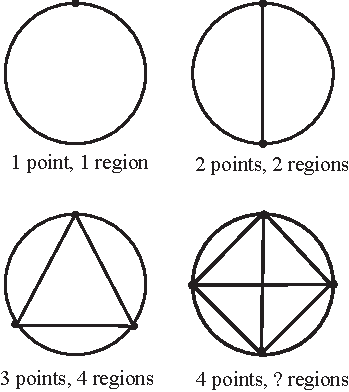
\includegraphics[width=\linewidth]{external/figps-circleregions.pdf}
\end{image}%
\tcblower
\end{figureptx}%
 Count the number of distinct regions within each circle. For example, with three points on the circle, there are four distinct regions. Organize your data in a table with two columns: ``Number of Points on the Circle'' and ``Number of Distinct Regions in the Circle.''%
\begin{enumerate}[font=\bfseries,label=(\alph*),ref=\alph*]
\item{}How many regions are there when there are four equally spaced points on the circle?%
\item\label{x:task:A_circleregions1}Based on the work so far, make a conjecture about how many distinct regions would you get with five equally spaced points.%
\item\label{x:task:A_circleregions2}Based on the work so far, make a conjecture about how many distinct regions would you get with six equally spaced points.%
\item{}\hyperref[x:figure:fig_circleregions56]{Figure~{\xreffont\ref{x:figure:fig_circleregions56}}, p.\,\pageref{x:figure:fig_circleregions56}} shows the figures associated with \hyperref[x:task:A_circleregions1]{Task~{\xreffont\ref{x:activity:exer_circleregions}}.{\xreffont\ref{x:task:A_circleregions1}}, p.\,\pageref{x:task:A_circleregions1}} and \hyperref[x:task:A_circleregions2]{Task~{\xreffont\ref{x:activity:exer_circleregions}}.{\xreffont\ref{x:task:A_circleregions2}}, p.\,\pageref{x:task:A_circleregions2}} Count the number of regions in each case. Are your conjectures correct or incorrect? \begin{figureptx}{Regions of Circles}{x:figure:fig_circleregions56}{}%
\begin{image}{0.275}{0.45}{0.275}%
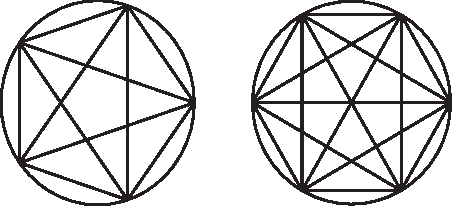
\includegraphics[width=\linewidth]{external/figps-circle5-6.pdf}
\end{image}%
\tcblower
\end{figureptx}%
%
\item{}Explain why this activity shows that the inductive step is an essential part of a proof by mathematical induction.%
\end{enumerate}
\end{activity}%
\end{exercises-subsection}
\end{sectionptx}
%
%
\typeout{************************************************}
\typeout{Section 4.2 Other Forms of Mathematical Induction}
\typeout{************************************************}
%
\begin{sectionptx}{Other Forms of Mathematical Induction}{}{Other Forms of Mathematical Induction}{}{}{x:section:S_otherinduction}
%
%
\typeout{************************************************}
\typeout{Beginning Activity  Beginning Activity 1: Exploring a Proposition about Factorials}
\typeout{************************************************}
%
\begin{worksheet-subsection}{Beginning Activity 1: Exploring a Proposition about Factorials}{}{Beginning Activity 1: Exploring a Proposition about Factorials}{}{}{x:worksheet:PA_factorials}
\begin{assemblage}{Definition.}{x:assemblage:nfactorial}%
\label{g:notation:idm824893992} If \(n\) is a natural number, we define \terminology{\(\boldsymbol{n}\) factorial}, denoted by \(n!\) , to be the product of the first \(n\) natural numbers. In addition, we define \(0!\) to be equal to 1.%
\end{assemblage}
Using this definition, we see that%
\begin{align*}
0! \amp = 1  \amp   3! \amp = 1 \cdot 2 \cdot 3 = 6\\
1! \amp =1   \amp   4! \amp = 1 \cdot 2 \cdot 3 \cdot 4 = 24\\
2! \amp = 1 \cdot 2 = 2  \amp   5! \amp = 1 \cdot 2 \cdot 3 \cdot 4 \cdot 5 = 120\text{.}
\end{align*}
%
\par
In general, we write \(n! = 1 \cdot 2 \cdot 3 \cdots \left( {n - 1} \right) \cdot n\) or \(n! = n \cdot \left( {n - 1} \right) \cdots 2 \cdot 1\). Notice that for any natural number \(n\), \(n! = n \cdot (n-1)!\).%
\begin{divisionexercise}{1}{}{}{x:exercise:pa_5211}%
Compute the values of \(2^n\) and \(n!\) for each natural number \(n\) with \(1 \leq n \leq 7\).%
\end{divisionexercise}%
Now let \(P(n)\) be the open sentence, ``\(n! > 2^n\).''%
\begin{divisionexercise}{2}{}{}{g:exercise:idm824882088}%
Which of the statements \(P(1)\) through \(P(7)\) are true?%
\end{divisionexercise}%
\begin{divisionexercise}{3}{}{}{x:exercise:pa_5212}%
Based on the evidence so far, does the following proposition appear to be true or false? For each natural number \(n\) with \(n \geq 4\), \(n! > 2^n\).%
\end{divisionexercise}%
Let \(k\) be a natural number with \(k \geq 4\). Suppose that we want to prove that if \(P(k)\) is true, then \(P(k+1)\) is true. (This could be the inductive step in an induction proof.) To do this, we would be assuming that \(k! > 2^k\) and would need to prove that \((k+1)! > 2^{k+1}\). Notice that if we multiply both sides of the inequality \(k! > 2^k\) by \((k + 1)\), we obtain%
\begin{equation}
(k + 1)\cdot k! > (k + 1) 2^k\text{.}\label{x:men:eq_otherinduct1}
\end{equation}
%
\begin{divisionexercise}{4}{}{}{x:exercise:pa_5214}%
In the inequality in \hyperref[x:men:eq_otherinduct1]{({\xreffont\ref{x:men:eq_otherinduct1}})}, explain why \((k + 1) \cdot k! = (k + 1)!\).%
\end{divisionexercise}%
\begin{divisionexercise}{5}{}{}{x:exercise:pa_5215}%
Now look at the right side of the inequality in \hyperref[x:men:eq_otherinduct1]{({\xreffont\ref{x:men:eq_otherinduct1}})} Since we are assuming that \(k \geq 4\), we can conclude that \((k+1) > 2\). Use this to help explain why \((k + 1)2^k > 2^{k+1}\).%
\end{divisionexercise}%
\begin{divisionexercise}{6}{}{}{g:exercise:idm824878760}%
Now use the inequality in (1) and the work in \hyperlink{x:exercise:pa_5214}{Exercise~{\xreffont 4}, p.\,\pageref{x:exercise:pa_5214}} and \hyperlink{x:exercise:pa_5215}{Exercise~{\xreffont 5}, p.\,\pageref{x:exercise:pa_5215}} to explain why \((k+1)! > 2^{k+1}\).%
\end{divisionexercise}%
\end{worksheet-subsection}
%
%
\typeout{************************************************}
\typeout{Beginning Activity  Beginning Activity 2: Prime Factors of a Natural Number}
\typeout{************************************************}
%
\begin{worksheet-subsection}{Beginning Activity 2: Prime Factors of a Natural Number}{}{Beginning Activity 2: Prime Factors of a Natural Number}{}{}{x:worksheet:PA_primefactors}
\index{prime number}%
\index{composite number}%
Recall that a natural number \(p\) is a \terminology{prime number} provided that it is greater than 1 and the only natural numbers that divide \(p\) are 1 and \(p\). A natural number other than 1 that is not a prime number is a \terminology{composite number}. The number 1 is neither prime nor composite.%
\begin{divisionexercise}{1}{}{}{g:exercise:idm824869800}%
Give examples of four natural numbers that are prime and four natural numbers that are composite.%
\end{divisionexercise}%
\begin{divisionexercise}{2}{}{}{x:exercise:PA_primefactors2}%
Write each of the natural numbers 20, 40, 50, and 150 as a product of prime numbers.%
\end{divisionexercise}%
\begin{divisionexercise}{3}{}{}{g:exercise:idm824868008}%
Do you think that any composite number can be written as a product of prime numbers?%
\end{divisionexercise}%
\begin{divisionexercise}{4}{}{}{g:exercise:idm824869288}%
Write a useful description of what it means to say that a natural number is a composite number (other than saying that it is not prime).%
\end{divisionexercise}%
\begin{divisionexercise}{5}{}{}{g:exercise:idm824866984}%
Based on your work in \hyperlink{x:exercise:PA_primefactors2}{Exercise~{\xreffont 2}, p.\,\pageref{x:exercise:PA_primefactors2}}, do you think it would be possible to use induction to prove that any composite number can be written as a product of prime numbers?%
\end{divisionexercise}%
\end{worksheet-subsection}
%
%
\typeout{************************************************}
\typeout{Subsection  The Domino Theory}
\typeout{************************************************}
%
\begin{subsectionptx}{The Domino Theory}{}{The Domino Theory}{}{}{g:subsection:idm824866088}
\index{domino theory}%
Mathematical induction is frequently used to prove statements of the form%
\begin{equation}
\left( {\forall n \in \mathbb{N}} \right)\left( {P( n )} \right)\text{,}\label{x:men:eq_5f}
\end{equation}
where \(P( n )\) is an open sentence. This means that we are proving that every statement in the following infinite list is true.%
\begin{equation}
P( 1 ),P( 2 ),P( 3 ), \ldots\label{x:men:eq_5g}
\end{equation}
%
\par
The inductive step in a proof by induction is to prove that if one statement in this infinite list of statements is true, then the next statement in the list must be true. Now imagine that each statement in equation \hyperref[x:men:eq_5g]{({\xreffont\ref{x:men:eq_5g}})} is a domino in a chain of dominoes. When we prove the inductive step, we are proving that if one domino is knocked over, then it will knock over the next one in the chain. Even if the dominoes are set up so that when one falls, the next one will fall, no dominoes will fall unless we start by knocking one over. This is why we need the basis step in an induction proof. The basis step guarantees that we knock over the first domino. The inductive step, then, guarantees that all dominoes after the first one will also fall.%
\par
Now think about what would happen if instead of knocking over the first domino, we knock over the sixth domino. If we also prove the inductive step, then we would know that every domino after the sixth domino would also fall. This is the idea of the \terminology{Extended Principle of Mathematical Induction}. It is not necessary for the basis step to be the proof that \(P( 1 )\) is true. We can make the basis step be the proof that \(P( M )\) is true, where \(M\) is some natural number. The Extended Principle of Mathematical Induction can be generalized somewhat by allowing \(M\) to be any integer. We are still only concerned with those integers that are greater than or equal to \(M\). \begin{assemblage}{The Extended Principle of Mathematical Induction.}{x:assemblage:principle-math-induct}%
Let \(M\) be an integer. If \(T\) is a subset of \(\mathbb{Z}\) such that%
\begin{enumerate}
\item{}\(M \in T\), and%
\item{}For every \(k \in \mathbb{Z}\) with \(k \geq M\), if \(k \in T\), then \(\left( {k + 1} \right) \in T\),%
\end{enumerate}
then \(T\) contains all integers greater than or equal to \(M\). That is, \(\left\{ n \in \mathbb{Z} \mid n \geq M \right\} \subseteq T\).%
\end{assemblage}
%
\end{subsectionptx}
%
%
\typeout{************************************************}
\typeout{Subsection  Using the Extended Principle of Mathematical Induction}
\typeout{************************************************}
%
\begin{subsectionptx}{Using the Extended Principle of Mathematical Induction}{}{Using the Extended Principle of Mathematical Induction}{}{}{g:subsection:idm824846632}
The primary use of the Principle of Mathematical Induction is to prove statements of the form%
\begin{equation*}
\left( {\forall n \in \mathbb{Z},\text{ with }  n \geq M} \right)\left( {P( n )} \right)\!\text{,}
\end{equation*}
where \(M\) is an integer and \(P( n )\) is some open sentence. (In most induction proofs, we will use a value of \(M\) that is greater than or equal to zero.) So our goal is to prove that the truth set \(T\) of the predicate \(P( n )\) contains all integers greater than or equal to \(M\). So to verify the hypothesis of the Extended Principle of Mathematical Induction, we must%
\begin{enumerate}
\item{}Prove that \(M \in T\). That is, prove that \(P( M )\) is true.%
\item{}Prove that for every \(k \in \mathbb{Z}\) with \(k \geq M\), if \(k \in T\), then \(\left( {k + 1} \right) \in T\). That is, prove that if \(P( k )\) is true, then \(P( {k + 1} )\) is true.%
\end{enumerate}
%
\par
\index{basis step}\index{mathematical induction!basis step}\index{inductive step}\index{mathematical induction!inductive step} As before, the first step is called the \terminology{basis step} or the \terminology{initial step}, and the second step is called the \terminology{inductive step}. This means that a proof using the Extended Principle of Mathematical Induction will have the following form:%
\begin{assemblage}{Using the Extended Principle of Mathematical Induction.}{x:assemblage:subsubsec-using-epmi}%
Let \(M\) be an integer. To prove: \(\left( {\forall n \in \mathbb{Z} \text{ with } n \geq M} \right)
\left( {P( n )} \right)\)%
\begin{descriptionlist}
\begin{dlimedium}{Basis step:}{g:li:idm824834088}%
Prove \(P( M )\).%
\end{dlimedium}%
\begin{dlimedium}{Inductive step:}{g:li:idm824831400}%
Prove that for every \(k \in \mathbb{Z}\) with \(k \geq M\), if \(P( k )\) is true, then \(P( {k + 1} )\) is true.%
\end{dlimedium}%
\end{descriptionlist}
%
\par
We can then conclude that \(P( n )\) is true for all \(n \in \mathbb{Z}\) with \(n \geq M\).%
\end{assemblage}
This is basically the same procedure as the one for using the Principle of Mathematical Induction. The only difference is that the basis step uses an integer \(M\) other than 1. For this reason, when we write a proof that uses the Extended Principle of Mathematical Induction, we often simply say we are going to use a proof by mathematical induction. We will use the work from \hyperref[x:worksheet:PA_factorials]{Beginning Activity 1, p.\,\pageref{x:worksheet:PA_factorials}} to illustrate such a proof.%
\begin{proposition}{}{}{x:proposition:P_factorialinduction}%
For each natural number \(n\) with \(n \geq 4\), \(n! > 2^n\).%
\end{proposition}
\begin{proof}{}{g:proof:idm824822440}
We will use a proof by mathematical induction. For this proof, we let \(P( n )\) be ``\(n! > 2^n\).'' We first prove that \(P( 4 )\) is true. Using \(n = 4\), we see that \(4! = 24\) and \(2^4 = 16\). This means that \(4! > 2^4\) and, hence, \(P\left( 4 \right)\) is true.%
\par
For the inductive step, we prove that for all \(k \in \mathbb{N}\) with \(k \geq 4\), if \(P( k )\) is true, then \(P( k + 1 )\) is true. So let \(k\) be a natural number greater than or equal to 4, and assume that \(P( k )\) is true. That is, assume that%
\begin{equation}
k! > 2^k\text{.}\label{x:men:eq_5h}
\end{equation}
%
\par
The goal is to prove that \(P( {k + 1} )\) is true or that \(\left( {k + 1} \right)! > 2^{k + 1}\). Multiplying both sides of inequality \hyperref[x:men:eq_5h]{({\xreffont\ref{x:men:eq_5h}})} by \(k + 1\) gives%
\begin{align}
\left( k + 1 \right) \cdot k! \amp > \left( k + 1 \right) 
\cdot 2^k ,\text{  or }\notag\\
\left( k + 1 \right)! \amp > \left( k + 1 \right) \cdot 2^k\label{x:mrow:eq_5i}
\end{align}
%
\par
Now, \(k \geq 4\). Thus, \(k + 1 > 2\), and hence \(\left( k + 1 \right) \cdot 2^k > 2 \cdot 2^k\). This means that%
\begin{equation}
\left( k + 1 \right) \cdot 2^k > 2^{k + 1}\text{.}\label{x:men:eq_5j}
\end{equation}
%
\par
Inequalities \hyperref[x:mrow:eq_5i]{({\xreffont\ref{x:mrow:eq_5i}})} and \hyperref[x:men:eq_5j]{({\xreffont\ref{x:men:eq_5j}})} show that%
\begin{equation*}
(k + 1)! > 2^{k + 1}\text{,}
\end{equation*}
and this proves that if \(P(k)\) is true, then \(P( {k + 1} )\) is true. Thus, the inductive step has been established, and so by the Extended Principle of Mathematical Induction, \(n! > 2^n\) for each natural number \(n\) with \(n \geq 4\).%
\end{proof}
\begin{inlineexercise}{Formulating Conjectures.}{x:exercise:prog_extendedind}%
Formulate a conjecture (with an appropriate quantifier) that can be used as an answer to each of the following questions.%
\begin{enumerate}[font=\bfseries,label=(\alph*),ref=\alph*]
\item{}For which natural numbers \(n\) is \(3^n\) greater than \(1 + 2^n\)?%
\space\hyperlink{g:solution:idm824806824-back}{[Solution]}\item{}For which natural numbers \(n\) is \(2^n\) greater than \(\left(n + 1 \right)^2\)?%
\space\hyperlink{g:solution:idm824808232-back}{[Solution]}\item{}For which natural numbers \(n\) is \(\left( 1 + \dfrac{1}{n} \right)^n\) greater than 2.5?%
\space\hyperlink{g:solution:idm824801448-back}{[Solution]}\end{enumerate}
\end{inlineexercise}%
\end{subsectionptx}
%
%
\typeout{************************************************}
\typeout{Subsection  The Second Principle of Mathematical Induction}
\typeout{************************************************}
%
\begin{subsectionptx}{The Second Principle of Mathematical Induction}{}{The Second Principle of Mathematical Induction}{}{}{g:subsection:idm824799784}
Let \(P( n )\) be \begin{quote}%
\(n\) is a prime number or \(n\) is a product of prime numbers.\end{quote}
 (This is related to the work in \hyperref[x:worksheet:PA_primefactors]{Beginning Activity 2, p.\,\pageref{x:worksheet:PA_primefactors}}.)%
\par
Suppose we would like to use induction to prove that \(P( n )\) is true for all natural numbers greater than 1. We have seen that the idea of the inductive step in a proof by induction is to prove that if one statement in an infinite list of statements is true, then the next statement must also be true. The problem here is that when we factor a composite number, we do not get to the previous case. For example, if assume that \(P(39)\) is true and we want to prove that \(P(40)\) is true, we could factor 40 as \(40 = 2 \cdot 20\). However, the assumption that \(P(39)\) is true does not help us prove that \(P(40)\) is true.%
\par
This work is intended to show the need for another principle of induction. In the inductive step of a proof by induction, we assume one statement is true and prove the next one is true. The idea of this new principle is to assume that \emph{all} of the previous statements are true and use this assumption to prove the next statement is true. This is stated formally in terms of subsets of natural numbers in the \terminology{Second Principle of Mathematical Induction}. Rather than stating this principle in two versions, we will state the extended version of the Second Principle. In many cases, we will use \(M = 1\) or \(M = 0\).%
\begin{assemblage}{The Second Principle of Mathematical Induction.}{x:assemblage:principle-math-induct2}%
Let \(M\) be an integer. If \(T\) is a subset of \(\mathbb{Z}\) such that%
\begin{enumerate}
\item{}\(M \in T\), and%
\item{}For every \(k \in \mathbb{Z}\) with \(k \geq M\), if \(\left\{ {M, M + 1, \ldots ,k} \right\} \subseteq T\), then \(\left( {k + 1} \right) \in T\),%
\end{enumerate}
then \(T\) contains all integers greater than or equal to \(M\). That is, \(\left\{ { {n \in \mathbb{Z} } \mid n \geq M} \right\} \subseteq T\).%
\end{assemblage}
\end{subsectionptx}
%
%
\typeout{************************************************}
\typeout{Subsection  Using the Second Principle of Mathematical Induction}
\typeout{************************************************}
%
\begin{subsectionptx}{Using the Second Principle of Mathematical Induction}{}{Using the Second Principle of Mathematical Induction}{}{}{g:subsection:idm824786984}
The primary use of mathematical induction is to prove statements of the form%
\begin{equation*}
\left( {\forall n \in \mathbb{Z},\text{ with } n \geq M} \right)\left( {P( n )} \right)\text{,}
\end{equation*}
where \(M\) is an integer and \(P( n )\) is some predicate. So our goal is to prove that the truth set \(T\) of the predicate \(P( n )\) contains all integers greater than or equal to \(M\). To use the Second Principle of Mathematical Induction, we must%
\begin{enumerate}
\item{}Prove that \(M \in T\). That is, prove that \(P( M )\) is true.%
\item{}Prove that for every \(k \in \mathbb{N}\), if \(k \geq M\) and \(\left\{ {M,M + 1, \ldots ,k} \right\} \subseteq T\), then \(\left( {k + 1} \right) \in T\). That is, prove that if \(P( M ),P( {M + 1} ), \ldots ,P( k )\) are true, then \(P( {k + 1} )\) is true.%
\end{enumerate}
%
\par
\index{basis step}\index{mathematical induction!basis step}\index{inductive step}\index{mathematical induction!inductive step} As before, the first step is called the \terminology{basis step} or the \terminology{initial step}, and the second step is called the \terminology{inductive step}. This means that a proof using the Second Principle of Mathematical Induction will have the following form:%
\begin{assemblage}{Using the Second Principle of Mathematical Induction.}{x:assemblage:using-secpmi}%
Let  \(M\)  be an integer.  To prove: \(\left( {\forall n \in \mathbb{Z} \text{ with }  n \geq M} \right)
\left( {P( n )} \right)\)%
\begin{descriptionlist}
\begin{dlimedium}{Basis step:}{g:li:idm824775080}%
Prove  \(P( M )\).%
\end{dlimedium}%
\begin{dlimedium}{Inductive step:}{g:li:idm824768936}%
Let \(k \in \mathbb{Z}\) with \(k \geq M\). Prove that if \(P( M ),P( {M + 1} ), \ldots ,P( k )\) are true, then \(P( {k + 1} )\) is true.%
\end{dlimedium}%
\end{descriptionlist}
%
\par
We can then conclude that \(P( n )\) is true for all \(n \in \mathbb{Z}\) with \(n \geq M\).%
\end{assemblage}
We will use this procedure to prove the proposition suggested in \hyperref[x:worksheet:PA_primefactors]{Beginning Activity 2, p.\,\pageref{x:worksheet:PA_primefactors}}.%
\begin{theorem}{}{}{x:theorem:T_primefactors}%
Each natural number greater than 1 either is a prime number or is a product of prime numbers.%
\end{theorem}
\begin{proof}{}{g:proof:idm824770600}
We will use the Second Principle of Mathematical Induction. We let \(P( n )\) be \(n\) is a prime number or \(n\) is a product of prime numbers.%
\par
For the basis step, \(P ( 2 )\) is true since 2 is a prime number.%
\par
To prove the inductive step, we let \(k\) be a natural number with \(k \geq 2\). We assume that \(P( 2 ),P( 3 ), \ldots ,P( k )\) are true. That is, we assume that each of the natural numbers \(2,3, \ldots ,k\) is a prime number or a product of prime numbers. The goal is to prove that \(P( {k + 1} )\) is true or that \((k + 1)\) is a prime number or a product of prime numbers.%
\par
Case 1: If \(\left( {k + 1} \right)\) is a prime number, then \(P( {k + 1} )\) is true.%
\par
Case 2: If \(\left( {k + 1} \right)\) is not a prime number, then \(\left( {k + 1} \right)\) can be factored into a product of natural numbers with each one being less than \(\left( {k + 1} \right)\). That is, there exist natural numbers \(a\) and \(b\) with%
\begin{equation*}
k + 1 = a \cdot b,  \text{ and }   1 \lt  a \leq k \text{ and }   1 \lt  b \leq k\text{.}
\end{equation*}
%
\par
Using the inductive assumption, this means that \(P( a )\) and \(P( b )\) are both true. Consequently, \(a\) and \(b\) are prime numbers or are products of prime numbers. Since \(k + 1 = a \cdot b\), we conclude that \(\left( {k + 1} \right)\) is a product of prime numbers. That is, we conclude that \(P\left( {k + 1} \right)\) is true. This proves the inductive step.%
\par
Hence, by the Second Principle of Mathematical Induction, we conclude that \(P( n )\) is true for all \(n \in \mathbb{N}\) with \(n \geq 2\), and this means that each natural number greater than 1 is either a prime number or is a product of prime numbers.%
\end{proof}
We will conclude this section with a progress check that is really more of an activity. We do this rather than including the activity at the end of the exercises since this activity illustrates a use of the Second Principle of Mathematical Induction in which it is convenient to have the basis step consist of the proof of more than one statement.%
\begin{inlineexercise}{Using the Second Principle of Induction.}{x:exercise:A_lincomb3and5-a}%
Consider the following question: \begin{quote}%
For which natural numbers \(n\) do there exist nonnegative integers \(x\) and \(y\) such that \(n = 3x + 5y\)?\end{quote}
 To help answer this question, we will let \(\mathbb{Z}^* = \left\{ {x \in \mathbb{Z} \mid x \geq 0} \right\}\), and let \(P \left( n \right)\) be There exist \(x,y \in \mathbb{Z}^*\) such that \(n = 3x + 5y\). Notice that \(P(1)\) is false since if both \(x\) and \(y\) are zero, then \(3x + 5y = 0\) and if either \(x > 0\) or \(y > 0\), then \(3x + 5y \geq 3\). Also notice that \(P(6)\) is true since \(6 = 3 \cdot 2 + 5 \cdot 0\) and \(P(8)\) is true since \(8 = 3 \cdot 1 + 5 \cdot 1\).%
\begin{enumerate}[font=\bfseries,label=(\alph*),ref=\alph*]
\item{}Explain why \(P(2)\), \(P(4)\), and \(P(7)\) are false and why \(P(3)\) and \(P(5)\) are true.%
\item{}Explain why \(P(9)\), \(P(10)\), \(P(11)\), and \(P(12)\) are true.%
\space\hyperlink{g:solution:idm824587816-back}{[Solution]}\item\label{x:task:A_lincombc}We could continue trying to determine other values of \(n\) for which \(P(n)\) is true. However, let us see if we can use the work in part~(2) to determine if \(P(13)\) is true. Notice that \(13 = 3 + 10\) and we know that \(P(10)\) is true. We should be able to use this to prove that \(P(13)\) is true. This is formalized in the next part.%
\par
Let \(k \in \mathbb{N}\) with \(k \geq 10\). Prove that if \(P( 8 )\), \(P ( 9 )\), \(\ldots\), \(P( k )\) are true, then \(P( {k+1} )\) is true.%
\item{}Prove the following proposition using mathematical induction. Use the Second Principle of Induction and have the basis step be a proof that \(P(8)\), \(P(9)\), and \(P(10)\) are true. (The inductive step is \hyperref[x:task:A_lincombc]{Task~{\xreffont\ref{x:exercise:A_lincomb3and5-a}}.{\xreffont\ref{x:task:A_lincombc}}, p.\,\pageref{x:task:A_lincombc}}.) \begin{proposition}{}{}{x:proposition:prop_lincomb}%
For each \(n \in \mathbb{N}\) with \(n \geq 8\), there exist nonnegative integers \(x\) and \(y\) such that \(n = 3x + 5y\).%
\end{proposition}
%
\space\hyperlink{g:solution:idm824557864-back}{[Solution]}\end{enumerate}
\end{inlineexercise}%
\end{subsectionptx}
%
%
\typeout{************************************************}
\typeout{Exercises  Exercises}
\typeout{************************************************}
%
\begin{exercises-subsection}{Exercises}{}{Exercises}{}{}{g:exercises:idm824541992}
\begin{divisionexercise}{1}{}{}{x:exercise:exer_sec52-1}%
Use mathematical induction to prove each of the following:%
\begin{enumerate}[font=\bfseries,label=(\alph*),ref=\alph*]
\item{}For each natural number \(n\) with \(n \geq 2\), \(3^n > 1 + 2^n\).%
\space\hyperlink{g:answer:idm824535720-back}{[Answer]}\item{}For each natural number \(n\) with \(n \geq 6\), \(2^n > \left( n + 1 \right)^2\).%
\item{}For each natural number \(n\) with \(n \geq 3\), \(\left( {1 + \dfrac{1}{n}} \right)^n \lt n\).%
\end{enumerate}
\end{divisionexercise}%
\begin{divisionexercise}{2}{}{}{x:exercise:exer_sec52-6}%
For which natural numbers \(n\) is \(n^2 \lt 2^n\)? Justify your conclusion.%
\space\hyperlink{g:answer:idm824521640-back}{[Answer]}\end{divisionexercise}%
\begin{divisionexercise}{3}{}{}{g:exercise:idm824511400}%
For which natural numbers \(n\) is \(n! > 3^n\)? Justify your conclusion.%
\end{divisionexercise}%
\begin{divisionexercise}{4}{}{}{x:exercise:exer_sec52-2}%
Complete the following.%
\begin{enumerate}[font=\bfseries,label=(\alph*),ref=\alph*]
\item\label{x:task:exer_522a}Verify that \(\left( {1 - \dfrac{1}{4}} \right) = \dfrac{3} {4}\) and that \(\left( {1 - \dfrac{1}{4}} \right)\left( {1 - \dfrac{1}{9}} \right) = \dfrac{4} {6}\).%
\item\label{x:task:exer_522b}Verify that \(\left( {1 - \dfrac{1}{4}} \right)\left( {1 - \dfrac{1}{9}} \right)
\left( {1 - \dfrac{1}{{16}}} \right) = \dfrac{5}{8}\) and that \(\left( {1 - \dfrac{1}{4}} \right)\left( {1 - \dfrac{1}{9}} \right)
\left( {1 - \dfrac{1}{{16}}} \right)\left( {1 - \dfrac{1}{{25}}} \right) = 
\dfrac{6}{{10}}\).%
\item{}For \(n \in \mathbb{N}\) with \(n \geq 2\), make a conjecture about a formula for the product \(\left( {1 - \dfrac{1}{4}} \right) \left( {1 - \dfrac{1}{9}} \right)
\left( {1 - \dfrac{1}{{16}}} \right) \cdots \left( {1 - \dfrac{1}{{n^2 }}} \right)\).%
\item{}Based on your work in Part \hyperref[x:task:exer_522a]{Task~{\xreffont 4}.{\xreffont\ref{x:task:exer_522a}}, p.\,\pageref{x:task:exer_522a}} and \hyperref[x:task:exer_522b]{Task~{\xreffont 4}.{\xreffont\ref{x:task:exer_522b}}, p.\,\pageref{x:task:exer_522b}}, state a proposition and then use the Extended Principle of Mathematical Induction to prove your proposition.%
\end{enumerate}
\end{divisionexercise}%
\begin{divisionexercise}{5}{}{}{x:exercise:exer_sec52-3}%
Is the following proposition true or false? Justify your conclusion. \begin{quote}%
For each nonnegative integer \(n\), \(8^n \mid \left( {4n} \right)!\).\end{quote}
%
\space\hyperlink{g:answer:idm824509736-back}{[Answer]}\end{divisionexercise}%
\begin{divisionexercise}{6}{}{}{x:exercise:exer_sec51-12}%
Let \(y = \ln x\).%
\begin{enumerate}[font=\bfseries,label=(\alph*),ref=\alph*]
\item{}Determine \(\dfrac{{dy}}{{dx}}\), \(\dfrac{{d^2 y}}{{dx^2 }}\), \(\dfrac{{d^3 y}}{{dx^3 }}\), and \(\dfrac{{d^4 y}}{{dx^4 }}\).%
\item{}Let \(n\) be a natural number. Formulate a conjecture for a formula for \(\dfrac{{d^n y}}{{dx^n }}\). Then use mathematical induction to prove your conjecture.%
\end{enumerate}
\end{divisionexercise}%
\begin{divisionexercise}{7}{}{}{x:exercise:exer_sec52-7}%
For which natural numbers \(n\) do there exist nonnegative integers \(x\) and \(y\) such that \(n = 4x + 5y\)? Justify your conclusion.%
\end{divisionexercise}%
\begin{divisionexercise}{8}{}{}{x:exercise:exer_sec52-4}%
Can each natural number greater than or equal to 4 be written as the sum of at least two natural numbers, each of which is a 2 or a 3? Justify your conclusion. For example, \(7 = 2 + 2 + 3\), and \(17 = 2 + 2 + 2 + 2 + 3 + 3 + 3\).%
\space\hyperlink{g:answer:idm824496424-back}{[Answer]}\end{divisionexercise}%
\begin{divisionexercise}{9}{}{}{x:exercise:exer_sec52-5}%
Can each natural number greater than or equal to 6 be written as the sum of at least two natural numbers, each of which is a 2 or a 5? Justify your conclusion. For example, \(6 = 2 + 2 + 2\), \(9 = 2 + 2 + 5\), and \(17 = 2 + 5 + 5 + 5\).%
\end{divisionexercise}%
\begin{divisionexercise}{10}{}{}{g:exercise:idm824490536}%
Use mathematical induction to prove the following proposition: \begin{quote}%
Let \(x\) be a real number with \(x > 0\). Then for each natural number \(n\) with \(n \geq 2\), \(\left( {1 + x} \right)^n > 1 + nx\).\end{quote}
 Explain where the assumption that \(x > 0\) was used in the proof.%
\end{divisionexercise}%
\begin{divisionexercise}{11}{}{}{g:exercise:idm824484264}%
Prove that for each odd natural number \(n\) with \(n \geq 3\),%
\begin{equation*}
\left( {1 + \frac{1}{2}} \right) \left( {1 - \frac{1}{3}} \right) \left( {1 + \frac{1}{4}} \right) \cdots \left( {1 + \frac{{\left( { - 1} \right)^n }}{n}} \right) = 1\text{.}
\end{equation*}
%
\end{divisionexercise}%
\begin{divisionexercise}{12}{}{}{x:exercise:exer_2elementsubsets}%
Prove that for each natural number \(n\), any set with \(n\) elements has \(\dfrac{n \left( {n-1} \right)}{2}\) two-element subsets.%
\space\hyperlink{g:answer:idm824485160-back}{[Answer]}\end{divisionexercise}%
\begin{divisionexercise}{13}{}{}{g:exercise:idm824473512}%
Prove or disprove each of the following propositions:%
\begin{enumerate}[font=\bfseries,label=(\alph*),ref=\alph*]
\item{}For each \(n \in \N\), \(\dfrac{1}{1 \cdot 2} + \dfrac{1}{2 \cdot 3} + \cdots + \dfrac{1}{n (n + 1 )} = 
\dfrac{n}{n+1}\).%
\item{}For each natural number \(n\) with \(n \geq 3\),%
\begin{equation*}
\frac{1}{3 \cdot 4} + \frac{1}{4 \cdot 5} + \cdots + \frac{1}{n (n + 1 )} = \frac{n-2}{3n + 3}\text{.}
\end{equation*}
%
\item{}For each \(n \in \N\), \(1 \cdot 2 + 2 \cdot 3 + 3 \cdot 4 + \cdots + n (n + 1 ) = 
\dfrac{n (n + 1 ) (n + 2 )}{3}\).%
\end{enumerate}
\end{divisionexercise}%
\begin{divisionexercise}{14}{}{}{g:exercise:idm824476328}%
Is the following proposition true or false? Justify your conclusion. \begin{quote}%
For each natural number \(n\), \(\left( \dfrac{n^3}{3} + \dfrac{n^2}{2} + \dfrac{7n}{6} \right)\) is a natural number.\end{quote}
%
\end{divisionexercise}%
\begin{divisionexercise}{15}{}{}{g:exercise:idm824465960}%
Is the following proposition true or false? Justify your conclusion. \begin{quote}%
For each natural number \(n\), \(\left( \dfrac{n^5}{5} + \dfrac{n^4}{2} + \dfrac{n^3}{3} - \dfrac{n}{30} \right)\) is an integer.\end{quote}
%
\end{divisionexercise}%
\begin{divisionexercise}{16}{}{}{x:exercise:exer_specialFTA}%
Complete the following.%
\begin{enumerate}[font=\bfseries,label=(\alph*),ref=\alph*]
\item\label{x:task:exer_specialFTAa}Prove that if \(n \in \N\), then there exists an odd natural number \(m\) and a nonnegative integer \(k\) such that \(n = 2^k m\).%
\space\hyperlink{g:hint:idm824462248-back}{[Hint]}\item{}For each \(n \in \N\), prove that there is only one way to write \(n\) in the form described in \hyperref[x:task:exer_specialFTAa]{Task~{\xreffont 16}.{\xreffont\ref{x:task:exer_specialFTAa}}, p.\,\pageref{x:task:exer_specialFTAa}}. To do this, assume that \(n = 2^k m\) and \(n = 2^q p\) where \(m\) and \(p\) are odd natural numbers and \(k\) and \(q\) are nonnegative integers. Then prove that \(k = q\) and \(m = p\).%
\space\hyperlink{g:hint:idm824458024-back}{[Hint]}\end{enumerate}
\end{divisionexercise}%
\begin{divisionexercise}{17}{Evaluation of Proofs.}{}{g:exercise:idm824454056}%
See the instructions for \hyperlink{x:exercise:exer_proofeval}{Exercise~{\xreffont 19}, p.\,\pageref{x:exercise:exer_proofeval}} from \hyperref[x:section:S_directproof]{Section~{\xreffont\ref{x:section:S_directproof}}, p.\,\pageref{x:section:S_directproof}}.%
\begin{enumerate}[font=\bfseries,label=(\alph*),ref=\alph*]
\item{}%
\begin{descriptionlist}
\begin{dlinarrow}{Proposition}{g:li:idm824460456}%
For each natural number \(n\) with \(n \geq 2\), \(2^n > 1 + n\).%
\end{dlinarrow}%
\begin{dlinarrow}{Proof}{g:li:idm824458920}%
We let \(k\) be a natural number and assume that \(2^k > 1 + k\). Multiplying both sides of this inequality by 2, we see that \(2^{k+1} > 2 + 2k\). However, \(2 + 2k > 2 + k\) and, hence,%
\begin{equation*}
2^{k+1} > 1 + \left(k + 1 \right)\!\text{.}
\end{equation*}
By mathematical induction, we conclude that \(2^n > 1 + n\).%
\end{dlinarrow}%
\end{descriptionlist}
%
\item{}%
\begin{descriptionlist}
\begin{dlinarrow}{Proposition}{g:li:idm824446376}%
Each natural number greater than or equal to 6 can be written as the sum of natural numbers, each of which is a 2 or a 5.%
\end{dlinarrow}%
\begin{dlinarrow}{Proof}{g:li:idm824448040}%
We will use a proof by induction. For each natural number \(n\), we let \(P( n )\) be, ``There exist nonnegative integers \(x\) and \(y\) such that \(n = 2x + 5y\).'' Since%
\begin{align*}
6 \amp = 3 \cdot 2 + 0 \cdot 5  \amp   7 \amp = 2 + 5\\
8 \amp = 4 \cdot 2 + 0 \cdot 5  \amp   9 \amp = 2 \cdot 2 + 1 \cdot 5
\end{align*}
we see that \(P(6 ), P(7 ), P(8 )\), and \(P( 9 )\) are true.%
\par
We now suppose that for some natural number \(k\) with \(k \geq 10\) that \(P(6 ), P (7 ), \ldots, P (k )\) are true. Now%
\begin{equation*}
k + 1 = \left(k - 4 \right) + 5\text{.}
\end{equation*}
%
\par
Since \(k \geq 10\), we see that \(k - 4 \geq 6\) and, hence, \(P(k - 4 )\) is true. So \(k - 4 = 2x + 5y\) and, hence,%
\begin{align*}
k + 1 \amp = \left(2x + 5y \right) + 5\\
\amp = 2x + 5 \left(y + 1 \right)\!
\end{align*}
This proves that \(P(k + 1 )\) is true, and hence, by the Second Principle of Mathematical Induction, we have proved that for each natural number \(n\) with \(n \geq 6\), there exist nonnegative integers \(x\) and \(y\) such that \(n = 2x + 5y\).%
\end{dlinarrow}%
\end{descriptionlist}
%
\end{enumerate}
\end{divisionexercise}%
\begin{activity}{The Sum of the Angles of a Convex Quadrilateral.}{x:activity:exer_convexquads}%
There is a famous theorem in Euclidean geometry that states that the sum of the interior angles of a triangle is \(180^\circ\).%
\begin{enumerate}[font=\bfseries,label=(\alph*),ref=\alph*]
\item\label{x:task:exer_convexquadsa}Use the theorem about triangles to determine the sum of the angles of a convex quadrilateral.%
\space\hyperlink{g:hint:idm824432552-back}{[Hint]}\par\smallskip%
\noindent\textbf{\blocktitlefont Hint}.\label{g:hint:idm824432552}{}\hypertarget{g:hint:idm824432552}{}\quad{}Draw a convex quadrilateral and draw a diagonal.%
\item\label{x:task:exer_convexquadsb}Use the result in \hyperref[x:task:exer_convexquadsa]{Task~{\xreffont\ref{x:activity:exer_convexquads}}.{\xreffont\ref{x:task:exer_convexquadsa}}, p.\,\pageref{x:task:exer_convexquadsa}} to determine the sum of the angles of a convex pentagon.%
\item{}Use the result in \hyperref[x:task:exer_convexquadsb]{Task~{\xreffont\ref{x:activity:exer_convexquads}}.{\xreffont\ref{x:task:exer_convexquadsb}}, p.\,\pageref{x:task:exer_convexquadsb}} to determine the sum of the angles of a convex hexagon.%
\item{}Let \(n\) be a natural number with \(n \geq 3\). Make a conjecture about the sum of the angles of a convex polygon with \(n\) sides and use mathematical induction to prove your conjecture.%
\end{enumerate}
\end{activity}%
\begin{activity}{De Moivre's Theorem.}{g:activity:idm824432296}%
\index{De Moivre's Theorem}%
\index{de Moivre, Abraham}%
One of the most interesting results in trigonometry is De Moivre's Theorem, which relates the complex number \(i\) to the trigonometric functions. Recall that the number \(i\) is a complex number whose square is \(-1\), that is, \(i^2 = -1\). One version of the theorem can be stated as follows: \begin{quote}%
If \(x\) is a real number, then for each nonnegative integer \(n\), \(\left[ {\cos x + i(\sin x)} \right]^n  = \cos (nx) + i( {\sin (nx)} )\!\).\end{quote}
 This theorem is named after Abraham de Moivre (1667 \textemdash{} 1754), a French mathematician.%
\begin{enumerate}[font=\bfseries,label=(\alph*),ref=\alph*]
\item\label{x:task:act-demoivrea}The proof of De Moivre's Theorem requires the use of the trigonometric identities for the sine and cosine of the sum of two angles. Use the Internet or a book to find identities for \(\sin( \alpha + \beta)\) and \(\cos (\alpha + \beta)\).%
\item{}To get a sense of how things work, expand \(\left[ {\cos x + i(\sin x)} \right]^2\) and write the result in the form \(a + bi\). Then use the identities from \hyperref[x:task:act-demoivrea]{Task~{\xreffont\ref{g:activity:idm824432296}}.{\xreffont\ref{x:task:act-demoivrea}}, p.\,\pageref{x:task:act-demoivrea}} to prove that \(\left[ {\cos x + i(\sin x)} \right]^2 = \cos (2x) + i( {\sin (2x)} )\).%
\item{}Use mathematical induction to prove De Moivre's Theorem.%
\end{enumerate}
\end{activity}%
\end{exercises-subsection}
\end{sectionptx}
%
%
\typeout{************************************************}
\typeout{Section 4.3 Induction and Recursion}
\typeout{************************************************}
%
\begin{sectionptx}{Induction and Recursion}{}{Induction and Recursion}{}{}{x:section:S_recursion}
%
%
\typeout{************************************************}
\typeout{Beginning Activity  Beginning Activity 1: Recursively Defined Sequences}
\typeout{************************************************}
%
\begin{worksheet-subsection}{Beginning Activity 1: Recursively Defined Sequences}{}{Beginning Activity 1: Recursively Defined Sequences}{}{}{x:worksheet:PA_recursivesequences}
\index{sequence}%
In a proof by mathematical induction, we ``start with a first step'' and then prove that we can always go from one step to the next step. We can use this same idea to define a sequence as well. We can think of a \terminology{sequence} as an infinite list of numbers that are indexed by the natural numbers (or some infinite subset of \(\mathbb{N} \cup \left\{ 0 \right\}\)). We often write a sequence in the following form:%
\begin{equation*}
a_1, a_2, \ldots,a_n, \ldots\text{.}
\end{equation*}
%
\par
The number \(a_n\) is called the \(n^\text{ th }\) term of the sequence. One way to define a sequence is to give a specific formula for the \(n^\text{ th }\) term of the sequence such as \(a_n = \dfrac{1}{n}\).%
\par
\index{definition!by recursion}\index{recursive definition}\index{initial condition}\index{recurrence relation} Another way to define a sequence is to give a specific definition of the first term (or the first few terms) and then state, in general terms, how to determine \(a_{n + 1}\) in terms of \(n\) and the first \(n\) terms \(a_1 ,a_2 , \ldots ,a_n\). This process is known as \terminology{definition by recursion} and is  also called a \terminology{recursive definition}. The specific definition of the first term is called the \terminology{initial condition}, and the general definition of \(a_{n + 1}\) in terms of \(n\) and the first \(n\) terms \(a_1 ,a_2 , \ldots ,a_n\) is called the \terminology{recurrence relation}. (When more than one term is defined explicitly, we say that these are the initial conditions.) For example, we can define a sequence recursively as follows: \begin{quote}%
\(b_1 = 16\), and for each \(n \in \mathbb{N}\), \(b_{n + 1} = \dfrac{1}{2}b_n\).\end{quote}
%
\par
Using \(n = 1\) and then \(n = 2\), we then see that%
\begin{align*}
b_2 \amp = \frac{1}{2} b_1 \amp     b_3 \amp = \frac{1}{2} b_2\\
\amp = \frac{1}{2} \cdot 16 \amp     \amp = \frac{1}{2} \cdot 8\\
\amp = 8                    \amp     \amp = 4
\end{align*}
%
\begin{divisionexercise}{1}{}{}{x:exercise:PA_recursivesequences1}%
Calculate \(b_4\) through \(b_{10}\). What seems to be happening to the values of \(b_n\) as \(n\) gets larger?%
\end{divisionexercise}%
\begin{divisionexercise}{2}{}{}{x:exercise:PA_recursivesequences2}%
Define a sequence recursively as follows: \begin{quote}%
\(T_1 = 16\), and for each \(n \in \mathbb{N}\), \(T_{n + 1} = 16 + \dfrac{1}{2}T_n\).\end{quote}
 Then \(T_2 = 16 + \dfrac{1}{2} T_1 = 16 + 8 = 24\). Calculate \(T_3\) through \(T_{10}\). What seems to be happening to the values of \(T_n\) as \(n\) gets larger?%
\end{divisionexercise}%
The sequences in \hyperlink{x:exercise:PA_recursivesequences1}{Exercise~{\xreffont 1}, p.\,\pageref{x:exercise:PA_recursivesequences1}} and \hyperlink{x:exercise:PA_recursivesequences2}{Exercise~{\xreffont 2}, p.\,\pageref{x:exercise:PA_recursivesequences2}} can be generalized as follows: Let \(a\) and \(r\) be real numbers. Define two sequences recursively as follows: \begin{quote}%
\(a_1 = a\), and for each \(n \in \mathbb{N}\), \(a_{n + 1} = r \cdot a_n\).\end{quote}
 \begin{quote}%
\(S_1 = a\), and for each \(n \in \mathbb{N}\), \(S_{n + 1} = a + r \cdot S_n\).\end{quote}
%
\begin{divisionexercise}{3}{}{}{g:exercise:idm824395048}%
Determine formulas (in terms of \(a\) and \(r\)) for \(a_2\) through \(a_6\). What do you think \(a_n\) is equal to (in terms of \(a\), \(r\), and \(n\))?%
\end{divisionexercise}%
\begin{divisionexercise}{4}{}{}{g:exercise:idm824389928}%
Determine formulas (in terms of \(a\) and \(r\)) for \(S_2\) through \(S_6\). What do you think \(S_n\) is equal to (in terms of \(a\), \(r\), and \(n\))?%
\end{divisionexercise}%
\index{factorial} In \hyperref[x:worksheet:PA_factorials]{Beginning Activity 1, p.\,\pageref{x:worksheet:PA_factorials}} in \hyperref[x:section:S_otherinduction]{Section~{\xreffont\ref{x:section:S_otherinduction}}, p.\,\pageref{x:section:S_otherinduction}}, for each natural number \(n\), we defined \(n!\), read \terminology{\(n\) factorial}, as the product of the first \(n\) natural numbers. We also defined \(0!\) to be equal to 1. Now recursively define a sequence of numbers \(a_0 ,a_1 ,a_2 , \ldots\) as follows: \begin{quote}%
\(a_0 = 1\), and\end{quote}
 \begin{quote}%
for each nonnegative integer \(n\), \(a_{n + 1} = \left( {n + 1} \right) \cdot a_n\).\end{quote}
%
\par
Using \(n=0\), we see that this implies that \(a_1 =1 \cdot a_0 = 1 \cdot 1 = 1\). Then using \(n = 1\), we see that%
\begin{equation*}
a_2 = 2 a_1 = 2 \cdot 1 = 2\text{.}
\end{equation*}
%
\begin{divisionexercise}{5}{}{}{g:exercise:idm824380840}%
Calculate \(a_3, a_4, a_5\), and \(a_6\).%
\end{divisionexercise}%
\begin{divisionexercise}{6}{}{}{g:exercise:idm824377768}%
Do you think that it is possible to calculate \(a_{20}\) and \(a_{100}\)? Explain.%
\end{divisionexercise}%
\begin{divisionexercise}{7}{}{}{g:exercise:idm824372648}%
Do you think it is possible to calculate \(a_n\) for any natural number \(n\)? Explain.%
\end{divisionexercise}%
\begin{divisionexercise}{8}{}{}{g:exercise:idm824376232}%
Compare the values of \(a_0 ,a_1 ,a_2 ,a_3 ,a_4 ,a_5\), and \(a_6\) with those of \(0!,1!,2!,3!,4!,5!\), and \(6!\). What do you observe? We will use mathematical induction to prove a result about this sequence in \hyperlink{x:exercise:exer_sec51-factorial}{Exercise~{\xreffont 1}, p.\,\pageref{x:exercise:exer_sec51-factorial}}.%
\end{divisionexercise}%
\end{worksheet-subsection}
%
%
\typeout{************************************************}
\typeout{Beginning Activity  Beginning Activity 2: The Fibonacci Numbers}
\typeout{************************************************}
%
\begin{worksheet-subsection}{Beginning Activity 2: The Fibonacci Numbers}{}{Beginning Activity 2: The Fibonacci Numbers}{}{}{x:worksheet:PA_fibonaccinumbers}
\index{Fibonacci numbers}%
\label{g:notation:idm824371880}%
The \terminology{Fibonacci numbers} are a sequence of natural numbers \(f_1 ,f_2 ,f_3 , \ldots ,f_n , \ldots\) defined recursively as follows:%
\begin{itemize}[label=\textbullet]
\item{}\(f_1 = 1\) and \(f_2 = 1\), and%
\item{}For each natural number \(n\), \(f_{n + 2} = f_{n + 1} + f_n\).%
\end{itemize}
In words, the recursion formula states that for any natural number \(n\) with \(n \geq 3\), the \(n^{th}\) Fibonacci number is the sum of the two previous Fibonacci numbers. So we see that%
\begin{align*}
f_3  \amp = f_2  + f_1  = 1 + 1 = 2,\\
f_4  \amp = f_3  + f_2  = 2 + 1 = 3, \text{ and }\\
f_5  \amp = f_4  + f_3 = 3 + 2 = 5\text{.}
\end{align*}
%
\begin{divisionexercise}{1}{}{}{g:exercise:idm824366248}%
Calculate \(f_6\) through \(f_{20}\).%
\end{divisionexercise}%
\begin{divisionexercise}{2}{}{}{g:exercise:idm824365352}%
Which of the Fibonacci numbers \(f_1\) through \(f_{20}\) are even? Which are multiples of 3?%
\end{divisionexercise}%
\begin{divisionexercise}{3}{}{}{g:exercise:idm824356392}%
For \(n = 2\), \(n = 3\), \(n = 4\), and \(n = 5\), how is the sum of the first \((n - 1)\) Fibonacci numbers related to the \((n + 1)^{st}\) Fibonacci number?%
\end{divisionexercise}%
\begin{divisionexercise}{4}{}{}{g:exercise:idm824359080}%
Record any other observations about the values of the Fibonacci numbers or any patterns that you observe in the sequence of Fibonacci numbers. If necessary, compute more Fibonacci numbers.%
\end{divisionexercise}%
\end{worksheet-subsection}
%
%
\typeout{************************************************}
\typeout{Subsection  The Fibonacci Numbers}
\typeout{************************************************}
%
\begin{subsectionptx}{The Fibonacci Numbers}{}{The Fibonacci Numbers}{}{}{g:subsection:idm824355752}
\index{Leonardo of Pisa}%
The Fibonacci numbers form a famous sequence in mathematics that was investigated by Leonardo of Pisa (1170 \textemdash{} 1250), who is better known as Fibonacci. Fibonacci introduced this sequence to the Western world as a solution of the following problem: \begin{quote}%
Suppose that a pair of adult rabbits (one male, one female) produces a pair of rabbits (one male, one female) each month.  Also, suppose that newborn rabbits become adults in two months and produce another pair of rabbits.  Starting with one adult pair of rabbits, how many pairs of rabbits will be produced each month for one year?\end{quote}
%
\par
Since we start with one adult pair, there will be one pair produced the first month, and since there is still only one adult pair, one pair will also be produced in the second month (since the new pair produced in the first month is not yet mature). In the third month, two pairs will be produced, one by the original pair and one by the pair which was produced in the first month. In the fourth month, three pairs will be produced, and in the fifth month, five pairs will be produced.%
\par
The basic rule is that in a given month after the first two months, the number of adult pairs is the number of adult pairs one month ago plus the number of pairs born two months ago. This is summarized in \hyperref[x:table:T_fibonacci]{Table~{\xreffont\ref{x:table:T_fibonacci}}, p.\,\pageref{x:table:T_fibonacci}}, where the number of pairs produced is equal to the number of adult pairs, and the number of adult pairs follows the Fibonacci sequence of numbers that we developed in \hyperref[x:worksheet:PA_fibonaccinumbers]{Beginning Activity 2, p.\,\pageref{x:worksheet:PA_fibonaccinumbers}}.%
\begin{tableptx}{\textbf{Fibonacci Numbers}}{x:table:T_fibonacci}{}%
\centering%
{\tabularfont%
\begin{tabular}{ccccccccccc}
\multicolumn{1}{cB}{Months}&\multicolumn{1}{cB}{1}&\multicolumn{1}{cB}{2}&\multicolumn{1}{cB}{3}&\multicolumn{1}{cB}{4}&\multicolumn{1}{cB}{5}&\multicolumn{1}{cB}{6}&\multicolumn{1}{cB}{7}&\multicolumn{1}{cB}{8}&\multicolumn{1}{cB}{9}&10\tabularnewline\hrulethick
\multicolumn{1}{cB}{Adult Pairs}&\multicolumn{1}{cB}{1}&\multicolumn{1}{cB}{1}&\multicolumn{1}{cB}{2}&\multicolumn{1}{cB}{3}&\multicolumn{1}{cB}{5}&\multicolumn{1}{cB}{8}&\multicolumn{1}{cB}{13}&\multicolumn{1}{cB}{21}&\multicolumn{1}{cB}{34}&55\tabularnewline\hrulethin
\multicolumn{1}{cB}{Newborn Pairs}&\multicolumn{1}{cB}{1}&\multicolumn{1}{cB}{1}&\multicolumn{1}{cB}{2}&\multicolumn{1}{cB}{3}&\multicolumn{1}{cB}{5}&\multicolumn{1}{cB}{8}&\multicolumn{1}{cB}{13}&\multicolumn{1}{cB}{21}&\multicolumn{1}{cB}{34}&55\tabularnewline\hrulethin
\multicolumn{1}{cB}{Month-Old Pairs}&\multicolumn{1}{cB}{0}&\multicolumn{1}{cB}{1}&\multicolumn{1}{cB}{1}&\multicolumn{1}{cB}{2}&\multicolumn{1}{cB}{3}&\multicolumn{1}{cB}{5}&\multicolumn{1}{cB}{8}&\multicolumn{1}{cB}{13}&\multicolumn{1}{cB}{21}&34
\end{tabular}
}%
\end{tableptx}%
\index{Hemachandra, Acharya} Historically, it is interesting to note that Indian mathematicians were studying these types of numerical sequences well before Fibonacci. In particular, about fifty years before Fibonacci introduced his sequence, Acharya Hemachandra (sometimes spelled Hemchandra) (1089 \textemdash{} 1173) considered the following problem, which is from the biography of Hemachandra in the \href{https://mathshistory.st-andrews.ac.uk/Biographies/Hemchandra/}{MacTutor History of Mathematics Archive}\footnote{\nolinkurl{mathshistory.st-andrews.ac.uk/Biographies/Hemchandra}\label{g:fn:idm824336552}}. \begin{quote}%
Suppose we assume that lines are composed of syllables which are either short or long. Suppose also that each long syllable takes twice as long to articulate as a short syllable. A line of length \(n\) contains \(n\) units where each short syllable is one unit and each long syllable is two units. Clearly a line of length \(n\) units takes the same time to articulate regardless of how it is composed. Hemchandra asks: How many different combinations of short and long syllables are possible in a line of length \(n\)?\end{quote}
%
\par
This is an important problem in the Sanskrit language since Sanskrit meters are based on duration rather than on accent as in the English Language. The answer to this question generates a sequence similar to the Fibonacci sequence. Suppose that \(h_n\) is the number of patterns of syllables of length \(n\). We then see that \(h_1 = 1\) and \(h_2 = 2\). Now let \(n\) be a natural number and consider pattern of length \(n + 2\). This pattern either ends in a short syllable or a long syllable. If it ends in a short syllable and this syllable is removed, then there is a pattern of length \(n+1\), and there are \(h_{n+1}\) such patterns. Similarly, if it ends in a long syllable and this syllable is removed, then there is a pattern of length \(n\), and there are \(h_n\) such patterns. From this, we conclude that%
\begin{equation*}
h_{n+2} = h_{n+1} + h_n\text{.}
\end{equation*}
This actually generates the sequence 1, 2, 3, 5, 8, 13, 21, \textellipsis{}. For more information about Hemachandra, see the article ``Math for Poets and Drummers'' by Rachel Wells Hall in the February 2008 issue of \pubtitle{Math Horizons}.%
\par
\index{Fibonacci Quarterly} We will continue to use the Fibonacci sequence in this book. This sequence may not seem all that important or interesting. However, it turns out that this sequence occurs in nature frequently and has applications in computer science. There is even a scholarly journal, \pubtitle{The Fibonacci Quarterly}, devoted to the Fibonacci numbers.%
\par
The sequence of Fibonacci numbers is one of the most studied sequences in mathematics, due mainly to the many beautiful patterns it contains. Perhaps one observation you made in \hyperref[x:worksheet:PA_fibonaccinumbers]{Beginning Activity 2, p.\,\pageref{x:worksheet:PA_fibonaccinumbers}} is that every third Fibonacci number is even. This can be written as a proposition as follows:%
\begin{equation*}
\text{ For each natural number }  n, f_{3n} \text{ is an even natural number }\text{.}
\end{equation*}
As with many propositions associated with definitions by recursion, we can prove this using mathematical induction. The first step is to define the appropriate open sentence. For this, we can let \(P(n)\) be, ``\(f_{3n}\) is an even natural number.''%
\par
Notice that \(P( 1 )\) is true since \(f_3 = 2\). We now need to prove the inductive step. To do this, we need to prove that for each \(k \in \mathbb{N}\), \begin{quote}%
if \(P( k )\) is true, then \(P( {k + 1} )\) is true.\end{quote}
 That is, we need to prove that for each \(k \in \mathbb{N}\), if \(f_{3k}\) is even, then \(f_{3\left( {k + 1} \right)}\) is even.%
\par
So let's analyze this conditional statement using a know-show table.%
\begin{center}%
{\tabularfont%
\begin{tabular}{lll}
\multicolumn{1}{lC}{\textbf{Step}}&\multicolumn{1}{lB}{\textbf{Know}}&\textbf{Reason}\tabularnewline\hrulemedium
\multicolumn{1}{lC}{\(P\)}&\multicolumn{1}{lB}{\(f_{3k}\)  is even.}&Inductive hypothesis\tabularnewline\hrulemedium
\multicolumn{1}{lC}{\(P1\)}&\multicolumn{1}{lB}{\(\left( {\exists m \in \mathbb{N}} \right)\left( {f_{3k}  = 2m} \right)\)}&Definition of ``even integer''\tabularnewline\hrulemedium
\multicolumn{1}{lC}{\(\vdots\)}&\multicolumn{1}{lB}{\(\vdots\)}&\(\vdots\)\tabularnewline\hrulemedium
\multicolumn{1}{lC}{\(Q1\)}&\multicolumn{1}{lB}{\(\left( {\exists q \in \mathbb{N}} \right)
\left( {f_{3\left( {k + 1} \right)}  = 2q} \right)\)}&\tabularnewline\hrulethin
\multicolumn{1}{lC}{\(Q\)}&\multicolumn{1}{lB}{\(f_{3\left( {k + 1} \right)}\) is even.}&Definition of ``even integer''\tabularnewline\hrulemedium
\multicolumn{1}{lC}{Step}&\multicolumn{1}{lB}{Show}&Reason
\end{tabular}
}%
\end{center}%
The key question now is, ``Is there any relation between \(f_{3\left( {k + 1} \right)}\) and \(f_{3k}\)?'' We can use the recursion formula that defines the Fibonacci sequence to find such a relation.%
\par
The recurrence relation for the Fibonacci sequence states that a Fibonacci number (except for the first two) is equal to the sum of the two previous Fibonacci numbers. If we write \(3\left( {k + 1} \right) = 3k + 3\), then we get \(f_{3\left( {k + 1} \right)}  = f_{3k + 3}\). For \(f_{3k + 3}\), the two previous Fibonacci numbers are \(f_{3k + 2}\) and \(f_{3k + 1}\). This means that%
\begin{equation*}
f_{3k + 3}  = f_{3k + 2}  + f_{3k + 1}\!\text{.}
\end{equation*}
Using this and continuing to use the Fibonacci relation, we obtain the following:%
\begin{align*}
f_{3\left( {k + 1} \right)} \amp = f_{3k + 3}\\
\amp = f_{3k + 2}  + f_{3k + 1}\\
\amp = \left( {f_{3k + 1}  + f_{3k} } \right) + f_{3k + 1}\text{.}
\end{align*}
The preceding equation states that \(f_{3\left( {k + 1} \right)} = 2f_{3k + 1} + f_{3k}\). This equation can be used to complete the proof of the induction step.%
\begin{inlineexercise}{Every Third Fibonacci Number Is Even.}{x:exercise:prog_thirdfibonacci}%
Complete the proof of \hyperref[x:proposition:P_thirdfibonacci]{Proposition~{\xreffont\ref{x:proposition:P_thirdfibonacci}}, p.\,\pageref{x:proposition:P_thirdfibonacci}}. \begin{proposition}{}{}{x:proposition:P_thirdfibonacci}%
For each natural number \(n\), the Fibonacci number \(f_{3n}\) is an even natural number.%
\end{proposition}
%
\space\hyperlink{g:solution:idm824261672-back}{[Solution]}\end{inlineexercise}%
\end{subsectionptx}
%
%
\typeout{************************************************}
\typeout{Subsection  Geometric Sequences and Geometric Series}
\typeout{************************************************}
%
\begin{subsectionptx}{Geometric Sequences and Geometric Series}{}{Geometric Sequences and Geometric Series}{}{}{x:subsection:geomseq}
Let \(a,r \in \mathbb{R}\). The following sequence was introduced in \hyperref[x:worksheet:PA_recursivesequences]{Beginning Activity 1, p.\,\pageref{x:worksheet:PA_recursivesequences}}.%
%
\begin{align*}
\text{Initial condition:  } \amp a_1 = a\\
\text{Recurrence relation:  } \amp \text{For each } n \in \N, a_{n + 1} = 
r \cdot a_n\text{.}
\end{align*}
\index{geometric sequence}\index{sequence!geometric} This is a recursive definition for a \terminology{geometric sequence} with \terminology{initial term} \(a\) and (common) \terminology{ratio} \(r\). The basic idea is that the next term in the sequence is obtained by multiplying the previous term by the ratio \(r\). The work in \hyperref[x:worksheet:PA_recursivesequences]{Beginning Activity 1, p.\,\pageref{x:worksheet:PA_recursivesequences}} suggests that the following proposition is true. \begin{theorem}{}{}{x:theorem:P_geometricsequence}%
Let \(a, r \in \mathbb{R}\). If a geometric sequence is defined by \(a_1 = a\) and for each \(n \in \mathbb{N}\), \(a_{n + 1} = r \cdot a_n\), then for each \(n \in \mathbb{N}\), \(a_n = a \cdot r^{n - 1}\).%
\end{theorem}
 The proof of this proposition is \hyperlink{x:exercise:exer_geomseq}{Exercise~{\xreffont 6}, p.\,\pageref{x:exercise:exer_geomseq}}.%
\par
\index{geometric series} Another sequence that was introduced in \hyperref[x:worksheet:PA_recursivesequences]{Beginning Activity 1, p.\,\pageref{x:worksheet:PA_recursivesequences}} is related to geometric series and is defined as follows:%
\begin{align*}
\text{Initial condition:  } \amp S_1 = a\\
\text{Recurrence relation:  } \amp \text{For each } n \in \N, S_{n + 1} = 
a + r \cdot S_n\text{.}
\end{align*}
For each \(n \in \mathbb{N}\), the term \(S_n\) is a (finite) \terminology{geometric series} with \terminology{initial term} \(a\) and (common) \terminology{ratio} \(r\). The work in \hyperref[x:worksheet:PA_recursivesequences]{Beginning Activity 1, p.\,\pageref{x:worksheet:PA_recursivesequences}} suggests that the following proposition is true.%
\begin{theorem}{}{}{x:theorem:P_geometricseries}%
Let \(a, r \in \mathbb{R}\). If the sequence \(S_1 ,S_2 , \ldots ,S_n , \ldots\) is defined by \(S_1 = a\) and for each \(n \in \mathbb{N}\), \(S_{n + 1} = a + r \cdot S_n\), then for each \(n \in \mathbb{N}\), \(S_n = a + a \cdot r + a \cdot r^2 + \cdots + a \cdot r^{n - 1}\). That is, the geometric series \(S_n\) is the sum of the first \(n\) terms of the corresponding geometric sequence.%
\end{theorem}
The proof of \hyperref[x:theorem:P_geometricseries]{Theorem~{\xreffont\ref{x:theorem:P_geometricseries}}, p.\,\pageref{x:theorem:P_geometricseries}} is \hyperlink{x:exercise:exer_geomser}{Exercise~{\xreffont 7}, p.\,\pageref{x:exercise:exer_geomser}}. The recursive definition of a geometric series and \hyperref[x:theorem:P_geometricseries]{Theorem~{\xreffont\ref{x:theorem:P_geometricseries}}, p.\,\pageref{x:theorem:P_geometricseries}} give two different ways to look at geometric series. \hyperref[x:theorem:P_geometricseries]{Theorem~{\xreffont\ref{x:theorem:P_geometricseries}}, p.\,\pageref{x:theorem:P_geometricseries}} represents a geometric series as the sum of the first \(n\) terms of the corresponding geometric sequence. Another way to determine the sum of a geometric series is given in \hyperref[x:theorem:P_geometricseries2]{Theorem~{\xreffont\ref{x:theorem:P_geometricseries2}}, p.\,\pageref{x:theorem:P_geometricseries2}}, which gives a formula for the sum of a geometric series that does not use a summation. \begin{theorem}{}{}{x:theorem:P_geometricseries2}%
Let \(a, r \in \mathbb{R}\) and \(r \ne 1\). If the sequence \(S_1 ,S_2 , \ldots ,S_n , \ldots\) is defined by \(S_1 = a\) and for each \(n \in \mathbb{N}\), \(S_{n + 1} = a + r \cdot S_n\), then for each \(n \in \mathbb{N}\), \(S_n = a\left( {\dfrac{{1 - r^n }}{{1 - r}}} \right)\).%
\end{theorem}
%
\par
The proof of \hyperref[x:theorem:P_geometricseries2]{Theorem~{\xreffont\ref{x:theorem:P_geometricseries2}}, p.\,\pageref{x:theorem:P_geometricseries2}} is \hyperlink{x:exercise:exer_geometricseries2}{Exercise~{\xreffont 8}, p.\,\pageref{x:exercise:exer_geometricseries2}}.%
\end{subsectionptx}
%
%
\typeout{************************************************}
\typeout{Exercises  Exercises}
\typeout{************************************************}
%
\begin{exercises-subsection}{Exercises}{}{Exercises}{}{}{g:exercises:idm824223272}
\begin{divisionexercise}{1}{}{}{x:exercise:exer_sec51-factorial}%
For the sequence \(a_{0}, a_1 ,a_2 , \ldots , a_n , \ldots\) , assume that \(a_0 = 1\) and that for each \(n \in \mathbb{N} \cup \left\{ 0 \right\}\), \(a_{n + 1} = \left( {n + 1} \right)a_n\). Use mathematical induction to prove that for each \(n \in \mathbb{N} \cup \left\{ 0 \right\}\), \(a_n = n!\).%
\space\hyperlink{g:answer:idm824217768-back}{[Answer]}\end{divisionexercise}%
\begin{divisionexercise}{2}{}{}{x:exercise:exer_sec53-fib}%
Assume that \(f_1 ,f_2 , \ldots ,f_n , \ldots\) are the Fibonacci numbers. Prove each of the following:%
\begin{enumerate}[font=\bfseries,label=(\alph*),ref=\alph*]
\item{}For each \(n \in \mathbb{N}\), \(f_{4n}\) is a multiple of 3.%
\space\hyperlink{g:answer:idm824208808-back}{[Answer]}\item{}For each \(n \in \mathbb{N}\), \(f_{5n}\) is a multiple of 5.%
\item{}For each \(n \in \mathbb{N}\) with \(n \geq 2\), \(f_1 + f_2 + \cdots + f_{n - 1} = f_{n + 1} - 1\).%
\space\hyperlink{g:answer:idm824205480-back}{[Answer]}\item{}For each \(n \in \mathbb{N}\), \(f_1 + f_3 + \cdots + f_{2n - 1} = f_{2n}\).%
\item{}For each \(n \in \mathbb{N}\), \(f_2 + f_4 + \cdots + f_{2n} = f_{2n + 1} - 1\).%
\item\label{x:task:exer_sec53-fibf}For each \(n \in \mathbb{N}\), \(f_1^2 + f_2^2 + \cdots + f_n^2 = f_n f_{n + 1}\).%
\space\hyperlink{g:answer:idm824190632-back}{[Answer]}\item{}For each \(n \in \mathbb{N}\) such that \(n\not \equiv 0 \pmod 3\), \(f_n\) is an odd integer.%
\end{enumerate}
\end{divisionexercise}%
\begin{divisionexercise}{3}{}{}{g:exercise:idm824183976}%
Use the result in \hyperref[x:task:exer_sec53-fibf]{Task~{\xreffont 2}.{\xreffont\ref{x:task:exer_sec53-fibf}}, p.\,\pageref{x:task:exer_sec53-fibf}} of \hyperlink{x:exercise:exer_sec53-fib}{Exercise~{\xreffont 2}, p.\,\pageref{x:exercise:exer_sec53-fib}} to prove that%
\begin{equation*}
\frac{f_1^2  + f_2^2  +  \cdots  + f_n^2 + f_{n+1}^2}{f_1^2  + f_2^2  +  \cdots  
+ f_n^2} = 1 + \frac{f_{n+1}}{f_n}\text{.}
\end{equation*}
%
\end{divisionexercise}%
\begin{divisionexercise}{4}{}{}{x:exercise:exer_binet}%
The quadratic formula can be used to show that \(\alpha = \dfrac{1 + \sqrt{5}}{2}\) and \(\beta = \dfrac{1 - \sqrt{5}}{2}\) are the two real number solutions of the quadratic equation \(x^2 - x - 1 = 0\). Notice that this implies that%
\begin{align*}
\alpha^2 \amp = \alpha + 1, \text{ and }\\
\beta^2 \amp = \beta + 1\text{.}
\end{align*}
It may be surprising to find out that these two irrational numbers are closely related to the Fibonacci numbers.%
\begin{enumerate}[font=\bfseries,label=(\alph*),ref=\alph*]
\item\label{x:task:exer_bineta}Verify that \(f_1 = \dfrac{\alpha^1 - \beta^1}{\alpha - \beta}\) and that \(f_2 = \dfrac{\alpha^2 - \beta^2}{\alpha - \beta}\).%
\item{}(This part is optional, but it may help with the induction proof in \hyperref[x:task:exer_binetc]{Task~{\xreffont 4}.{\xreffont\ref{x:task:exer_binetc}}, p.\,\pageref{x:task:exer_binetc}}.) Work with the relation \(f_3 = f_2 + f_1\) and substitute the expressions for \(f_1\) and \(f_2\) from \hyperref[x:task:exer_bineta]{Task~{\xreffont 4}.{\xreffont\ref{x:task:exer_bineta}}, p.\,\pageref{x:task:exer_bineta}} Rewrite the expression as a single fraction and then in the numerator use \(\alpha^2 + \alpha = \alpha ( \alpha + 1 )\) and a similar equation involving \(\beta\). Now prove that \(f_3 = \dfrac{\alpha^3 - \beta^3}{\alpha - \beta}\).%
\item\label{x:task:exer_binetc}\index{Binet's formula}%
Use induction to prove that for each natural number \(n\), if \(\alpha = \dfrac{1 + \sqrt{5}}{2}\) and \(\beta = \dfrac{1 - \sqrt{5}}{2}\), then \(f_n = \dfrac{\alpha^n - \beta^n}{\alpha - \beta}\).%
\par
This formula for the \(n^{th}\) Fibonacci number is known as Binet's formula, named after the French mathematician Jacques Binet (1786 \textemdash{} 1856).%
\end{enumerate}
\end{divisionexercise}%
\begin{divisionexercise}{5}{}{}{g:exercise:idm824166952}%
Is the following conjecture true or false? \begin{conjecture}{}{}{g:conjecture:idm824170152}%
Let \(f_1, f_2, \ldots,
f_m, \ldots\) be the sequence of the Fibonacci numbers. For each natural number \(n\), the numbers \(f_nf_{n+3}\), \(2f_{n+1}f_{n+2}\), and \(\left( f_{n+1}^2 + f_{n+2}^2 \right)\) form a Pythagorean triple.%
\end{conjecture}
%
\end{divisionexercise}%
\begin{divisionexercise}{6}{}{}{x:exercise:exer_geomseq}%
Prove \hyperref[x:theorem:P_geometricsequence]{Theorem~{\xreffont\ref{x:theorem:P_geometricsequence}}, p.\,\pageref{x:theorem:P_geometricsequence}}. Let \(a,r \in \mathbb{R}\). If a geometric sequence is defined by \(a_1 = a\) and for each \(n \in \mathbb{N}\), \(a_{n + 1} = r \cdot a_n\), then for each \(n \in \mathbb{N}\), \(a_n = a \cdot r^{n - 1}\).%
\space\hyperlink{g:answer:idm824159400-back}{[Answer]}\end{divisionexercise}%
\begin{divisionexercise}{7}{}{}{x:exercise:exer_geomser}%
Prove \hyperref[x:theorem:P_geometricseries]{Theorem~{\xreffont\ref{x:theorem:P_geometricseries}}, p.\,\pageref{x:theorem:P_geometricseries}}. Let \(a,r \in \mathbb{R}\). If the sequence \(S_1 ,S_2 , \ldots ,S_n , \ldots\) is defined by \(S_1 = a\) and for each \(n \in \mathbb{N}\), \(S_{n + 1} = a + r \cdot S_n\), then for each \(n \in \mathbb{N}\), \(S_n = a + a \cdot r + a \cdot r^2 + \cdots + a \cdot r^{n - 1}\). That is, the geometric series \(S_n\) is the sum of the first \(n\) terms of the corresponding geometric sequence.%
\end{divisionexercise}%
\begin{divisionexercise}{8}{}{}{x:exercise:exer_geometricseries2}%
Prove \hyperref[x:theorem:P_geometricseries2]{Theorem~{\xreffont\ref{x:theorem:P_geometricseries2}}, p.\,\pageref{x:theorem:P_geometricseries2}}. Let \(a, r \in \mathbb{R}\) and \(r \ne 1\). If the sequence \(S_1 ,S_2 , \ldots ,S_n , \ldots\) is defined by \(S_1 = a\) and for each \(n \in \mathbb{N}\), \(S_{n + 1} = a + r \cdot S_n\), then for each \(n \in \mathbb{N}\), \(S_n = a\left( {\dfrac{{1 - r^n }}{{1 - r}}} \right)\).%
\space\hyperlink{g:answer:idm824149928-back}{[Answer]}\end{divisionexercise}%
\begin{divisionexercise}{9}{}{}{x:exercise:exer_sec53-arithexample}%
For the sequence \(a_1 ,a_2 , \ldots ,a_n , \ldots\) , assume that \(a_1 = 2\) and that for each \(n \in \mathbb{N}\), \(a_{n + 1} = a_n + 5\).%
\begin{enumerate}[font=\bfseries,label=(\alph*),ref=\alph*]
\item{}Calculate \(a_2\) through \(a_6\).%
\space\hyperlink{g:answer:idm824150056-back}{[Answer]}\item\label{x:task:exer_sec53-arithexampleb}Make a conjecture for a formula for \(a_n\) for each \(n \in \mathbb{N}\).%
\space\hyperlink{g:answer:idm824145704-back}{[Answer]}\item{}Prove that your conjecture in \hyperref[x:task:exer_sec53-arithexampleb]{Task~{\xreffont 9}.{\xreffont\ref{x:task:exer_sec53-arithexampleb}}, p.\,\pageref{x:task:exer_sec53-arithexampleb}} is correct.%
\end{enumerate}
\end{divisionexercise}%
\begin{divisionexercise}{10}{}{}{x:exercise:exer_sec53-arith}%
\index{arithmetic sequence}%
\index{sequence!arithmetic}%
The sequence in \hyperlink{x:exercise:exer_sec53-arithexample}{Exercise~{\xreffont 9}, p.\,\pageref{x:exercise:exer_sec53-arithexample}} is an example of an \terminology{arithmetic sequence}. An arithmetic sequence is defined recursively as follows: \begin{quote}%
Let \(c\) and \(d\) be real numbers. Define the sequence \(a_1 ,a_2 , \ldots ,a_n , \ldots\) by \(a_1 = c\) and for each \(n \in \mathbb{N}\), \(a_{n + 1} = a_n + d\).\end{quote}
%
\begin{enumerate}[font=\bfseries,label=(\alph*),ref=\alph*]
\item{}Determine formulas for \(a_3\) through \(a_8\).%
\item\label{x:task:exer_sec53-arithb}Make a conjecture for a formula for \(a_n\) for each \(n \in \mathbb{N}\).%
\item{}Prove that your conjecture in \hyperref[x:task:exer_sec53-arithb]{Task~{\xreffont 10}.{\xreffont\ref{x:task:exer_sec53-arithb}}, p.\,\pageref{x:task:exer_sec53-arithb}} is correct.%
\end{enumerate}
\end{divisionexercise}%
\begin{divisionexercise}{11}{}{}{g:exercise:idm824135336}%
For the sequence \(a_1 ,a_2 , \ldots ,a_n , \ldots\) , assume that \(a_1 = 1\), \(a_2 = 5\), and that for each \(n \in \mathbb{N}\) with \(n\geq 2\), \(a_{n + 1} = a_n + 2a_{n-1}\). Prove that for each natural number \(n\), \(a_n = 2^n + (-1)^n\).%
\end{divisionexercise}%
\begin{divisionexercise}{12}{}{}{x:exercise:exer_sec53-5}%
For the sequence \(a_1 ,a_2 , \ldots ,a_n , \ldots\) , assume that \(a_1 = 1\) and that for each \(n \in \mathbb{N}\), \(a_{n + 1} = \sqrt {5 + a_n }\).%
\begin{enumerate}[font=\bfseries,label=(\alph*),ref=\alph*]
\item{}Calculate, or approximate, \(a_2\) through \(a_6\).%
\space\hyperlink{g:answer:idm824125480-back}{[Answer]}\item{}Prove that for each \(n \in \mathbb{N}\), \(a_n \lt 3\).%
\space\hyperlink{g:answer:idm824126632-back}{[Answer]}\end{enumerate}
\end{divisionexercise}%
\begin{divisionexercise}{13}{}{}{x:exercise:exer_sec53-6}%
For the sequence \(a_1 ,a_2 , \ldots ,a_n , \ldots\) , assume that \(a_1 = 1\), \(a_2 = 3\), and that for each \(n \in \mathbb{N}\), \(a_{n + 2} = 3a_{n + 1} - 2a_n\).%
\begin{enumerate}[font=\bfseries,label=(\alph*),ref=\alph*]
\item{}Calculate \(a_3\) through \(a_6\).%
\space\hyperlink{g:answer:idm824108968-back}{[Answer]}\item\label{x:task:exer_536b}Make a conjecture for a formula for \(a_n\) for each \(n \in \mathbb{N}\).%
\space\hyperlink{g:hint:idm824115496-back}{[Hint]}\item{}Prove that your conjecture in \hyperref[x:task:exer_536b]{Task~{\xreffont 13}.{\xreffont\ref{x:task:exer_536b}}, p.\,\pageref{x:task:exer_536b}} is correct.%
\end{enumerate}
\end{divisionexercise}%
\begin{divisionexercise}{14}{}{}{x:exercise:exer_sec53-7}%
For the sequence \(a_1 ,a_2 , \ldots ,a_n , \ldots\) , assume that \(a_1 = 1\), \(a_2 = 1\), and that for each \(n \in \mathbb{N}\), \(a_{n + 2} = \dfrac{1}{2}\left( {a_{n + 1} + \dfrac{2}{{a_n }}} \right)\).%
\begin{enumerate}[font=\bfseries,label=(\alph*),ref=\alph*]
\item{}Calculate \(a_3\) through \(a_6\).%
\space\hyperlink{g:answer:idm824108712-back}{[Answer]}\item{}Prove that for each \(n \in \mathbb{N}\), \(1 \leq a_n \leq 2\).%
\end{enumerate}
\end{divisionexercise}%
\begin{divisionexercise}{15}{}{}{x:exercise:exer_sec53-8}%
For the sequence   \(a_1 ,a_2 , \ldots ,a_n , \ldots\), assume that \(a_1=1\), \(a_2=1\), \(a_3=1\), and for that each natural number \(n\),%
\begin{equation*}
a_{n+3} = a_{n+2} + a_{n+1} + a_n\text{.}
\end{equation*}
%
\begin{enumerate}[font=\bfseries,label=(\alph*),ref=\alph*]
\item{}Compute \(a_4\), \(a_5\), \(a_6\), and \(a_7\).%
\item{}Prove that for each natural number \(n\) with \(n>1\), \(a_n \leq 2^{n-2}\).%
\end{enumerate}
\end{divisionexercise}%
\begin{divisionexercise}{16}{}{}{x:exercise:exer_factorial}%
For the sequence \(a_1, a_2, \ldots, a_n, \ldots\), assume that \(a_1 = 1\), and that for each natural number \(n\),%
\begin{equation*}
a_{n + 1} = a_n + n \cdot n!\text{.}
\end{equation*}
%
\begin{enumerate}[font=\bfseries,label=(\alph*),ref=\alph*]
\item{}Compute \(n!\) for the first 10 natural numbers.%
\item{}Compute \(a_n\) for the first 10 natural numbers.%
\space\hyperlink{g:answer:idm824094504-back}{[Answer]}\item\label{x:task:exer_factorialc}Make a conjecture about a formula for \(a_n\) in terms of \(n\) that does not involve a summation or a recursion.%
\item{}Prove your conjecture in \hyperref[x:task:exer_factorialc]{Task~{\xreffont 16}.{\xreffont\ref{x:task:exer_factorialc}}, p.\,\pageref{x:task:exer_factorialc}}.%
\end{enumerate}
\end{divisionexercise}%
\begin{divisionexercise}{17}{}{}{g:exercise:idm824087336}%
For the sequence \(a_1, a_2, \ldots,
a_n, \ldots\) , assume that \(a_1 = 1\), \(a_2 = 1\), and for each \(n \in \N\), \(a_{n+2} = a_{n+1} + 3a_n\). Determine which terms in this sequence are divisible by 4 and prove that your answer is correct.%
\end{divisionexercise}%
\begin{divisionexercise}{18}{}{}{x:exercise:exer_lucasnumbers}%
\index{Lucas numbers}%
The \terminology{Lucas numbers} are a sequence of natural numbers \(L_1, L_2, L_3, \ldots, L_n, \ldots \), which are defined recursively as follows:%
\begin{itemize}[label=\textbullet]
\item{}\(L_1 = 1\) and \(L_2 = 3\), and%
\item{}For each natural number \(n\), \(L_{n+2} = L_{n+1} + L_n\).%
\end{itemize}
List the first 10 Lucas numbers and the first ten Fibonacci numbers and then prove each of the following propositions. The Second Principle of Mathematical Induction may be needed to prove some of these propositions.%
\begin{enumerate}[font=\bfseries,label=(\alph*),ref=\alph*]
\item{}For each natural number \(n\), \(L_n = 2f_{n+1} - f_n\).%
\space\hyperlink{g:answer:idm824078248-back}{[Answer]}\item{}For each \(n \in \mathbb{N}\) with \(n \geq 2\), \(5f_n = L_{n - 1} + L_{n + 1}\).%
\item{}For each \(n \in \mathbb{N}\) with \(n \geq 3\), \(L_n = f_{n + 2} - f_{n - 2}\).%
\end{enumerate}
\end{divisionexercise}%
\begin{divisionexercise}{19}{}{}{x:exercise:exer_lucasnumbers2}%
There is a formula for the Lucas numbers similar to the formula for the Fibonacci numbers in \hyperlink{x:exercise:exer_binet}{Exercise~{\xreffont 4}, p.\,\pageref{x:exercise:exer_binet}}. Let \(\alpha = \dfrac{1 + \sqrt{5}}{2}\) and \(\beta = \dfrac{1 - \sqrt{5}}{2}\). Prove that for each \(n \in \N\), \(L_n = \alpha^n + \beta^n\).%
\end{divisionexercise}%
\begin{divisionexercise}{20}{}{}{g:exercise:idm824073000}%
Use the result in \hyperlink{x:exercise:exer_lucasnumbers2}{Exercise~{\xreffont 19}, p.\,\pageref{x:exercise:exer_lucasnumbers2}}, previously proven results from \hyperlink{x:exercise:exer_lucasnumbers}{Exercise~{\xreffont 18}, p.\,\pageref{x:exercise:exer_lucasnumbers}}, or mathematical induction to prove each of the following results about Lucas numbers and Fibonacci numbers.%
\begin{enumerate}[font=\bfseries,label=(\alph*),ref=\alph*]
\item{}For each \(n \in \mathbb{N}\), \(L_n = \dfrac{{f_{2n} }}{{f_n }}\).%
\item{}For each \(n \in \mathbb{N}\), \(f_{n+1} = \dfrac{f_n + L_n}{2}\).%
\item{}For each \(n \in \mathbb{N}\), \(L_{n+1} = \dfrac{L_n +5f_n}{2}\).%
\item{}For each \(n \in \mathbb{N}\) with \(n \geq 2\), \(L_n = f_{n+1} + f_{n-1}\).%
\end{enumerate}
\end{divisionexercise}%
\begin{divisionexercise}{21}{Evaluation of Proofs.}{}{g:exercise:idm824062888}%
See the instructions for \hyperlink{x:exercise:exer_proofeval}{Exercise~{\xreffont 19}, p.\,\pageref{x:exercise:exer_proofeval}} from \hyperref[x:section:S_directproof]{Section~{\xreffont\ref{x:section:S_directproof}}, p.\,\pageref{x:section:S_directproof}}.%
\begin{enumerate}[font=\bfseries,label=(\alph*),ref=\alph*]
\item{}%
\begin{descriptionlist}
\begin{dlinarrow}{Proposition}{g:li:idm824059944}%
Let \(f_n\) be the \(n^\text{ th }\) Fibonacci number, and let \(\alpha\) be the positive solution of the equation \(x^2 = x + 1\). So \(\alpha = \dfrac{1 + \sqrt{5}}{2}\). For each natural number \(n\), \(f_n \leq \alpha^{n-1}\).%
\end{dlinarrow}%
\begin{dlinarrow}{Proof}{g:li:idm824056232}%
We will use a proof by mathematical induction. For each natural number \(n\), we let \(P( n )\) be, ``\(f_n \leq \alpha^{n-1}\).''%
\par
We first note that \(P( 1 )\) is true since \(f_1 = 1\) and \(\alpha^0 = 1\). We also notice that \(P( 2 )\) is true since \(f_2 = 1\) and, hence, \(f_2 \leq \alpha^1\).%
\par
We now let \(k\) be a natural number with \(k \geq 2\) and assume that \(P ( 1 )\), \(P( 2 )\), \textellipsis{} , \(P( k )\) are all true. We now need to prove that \(P \left( k + 1 \right)\) is true or that \(f_{k+1} \leq \alpha^k\).%
\par
Since \(P( k -1 )\) and \(P ( k )\) are true, we know that \(f_{k-1} \leq \alpha^{k-2}\) and \(f_k \leq \alpha^{k-1}\). Therefore,%
\begin{align*}
f_{k + 1} \amp = f_k + f_{k-1}\\
f_{k + 1} \amp \leq \alpha^{k-1} + \alpha^{k-2}\\
f_{k + 1} \amp \leq \alpha^{k-2} \left(\alpha + 1 \right)\!\text{.}
\end{align*}
We now use the fact that \(\alpha + 1 = \alpha^2\) and the preceding inequality to obtain%
\begin{align*}
f_{k+1} \amp \leq \alpha^{k-2} \alpha^2\\
f_{k+1} \amp \leq \alpha^k
\end{align*}
This proves that if \(P( 1 )\), \(P( 2 )\), \textellipsis{} , \(P( k )\) are true, then \(P(k + 1 )\) is true. Hence, by the Second Principle of Mathematical Induction, we conclude that for each natural number \(n\), \(f_n \leq \alpha^{n-1}\).%
\end{dlinarrow}%
\end{descriptionlist}
%
\end{enumerate}
\end{divisionexercise}%
\begin{activity}{Compound Interest.}{x:activity:exer_compoundinterest}%
\index{compound interest}%
Assume that  \(R\)  dollars is deposited in an account that has an interest rate of  \(i\)  for each compounding period. A compounding period is some specified time period such as a month or a year. For each integer  \(n\)  with  \(n \geq 0\), let  \(V_n\) be the amount of money in an account at the end of the \(n\)th compounding period. Then%
\begin{align*}
V_1 \amp = R + i \cdot R \amp V_2 \amp = V_1 + i \cdot V_1\\
\amp = R \left( 1 + i \right) \amp \amp = \left( {1 + i} \right) V_1\\
\amp \amp \amp = \left( {1 + i} \right)^2 R\text{.}
\end{align*}
%
\begin{enumerate}[font=\bfseries,label=(\alph*),ref=\alph*]
\item{}Explain why \(V_3 = V_2 + i \cdot V_2\). Then use the formula for \(V_2\) to determine a formula for \(V_3\) in terms of \(i\) and \(R\).%
\item\label{x:task:A_compoundinterest2}Determine a recurrence relation for \(V_{n + 1}\) in terms of \(i\) and \(V_n\).%
\item{}Write the recurrence relation in \hyperref[x:task:A_compoundinterest2]{Task~{\xreffont\ref{x:activity:exer_compoundinterest}}.{\xreffont\ref{x:task:A_compoundinterest2}}, p.\,\pageref{x:task:A_compoundinterest2}} so that it is in the form of a recurrence relation for a geometric sequence. What is the initial term of the geometric sequence and what is the common ratio?%
\item{}Use \hyperref[x:theorem:P_geometricsequence]{Theorem~{\xreffont\ref{x:theorem:P_geometricsequence}}, p.\,\pageref{x:theorem:P_geometricsequence}} to determine a formula for \(V_n\) in terms of \(I\), \(R\), and \(n\).%
\end{enumerate}
\end{activity}%
\begin{activity}{The Future Value of an Ordinary Annuity.}{x:activity:exer_annuity}%
\index{ordinary annuity}%
\index{future value}%
For an \terminology{ordinary annuity}, \(R\) dollars is deposited in an account at the end of each compounding period. It is assumed that the interest rate, \(i\), per compounding period for the account remains constant. Let \(S_t\) represent the amount in the account at the end of the \(t\)th compounding period. \(S_t\) is frequently called the \terminology{future value} of the ordinary annuity. So  \(S_1  = R\). To determine the amount after two months, we first note that the amount after one month will gain interest and grow to \(( {1 + i} )S_1\). In addition, a new deposit of  \(R\)  dollars will be made at the end of the second month. So%
\begin{equation*}
S_2  = R + ( {1 + i} )S_1\text{.}
\end{equation*}
%
\begin{enumerate}[font=\bfseries,label=(\alph*),ref=\alph*]
\item{}For each \(n \in \mathbb{N}\), use a similar argument to determine a recurrence relation for \(S_{n + 1}\) in terms of \(R\), \(i\), and \(S_n\).%
\item{}By recognizing this as a recursion formula for a geometric series, use \hyperref[x:theorem:P_geometricseries2]{Theorem~{\xreffont\ref{x:theorem:P_geometricseries2}}, p.\,\pageref{x:theorem:P_geometricseries2}} to determine a formula for  \(S_n\) in terms of  \(R\), \(i\), and  \(n\)  that does not use a summation. Then show that this formula can be written as%
\begin{equation*}
S_n  = R\left( {\frac{{\left( {1 + i} \right)^n  - 1}}{i}} \right)\text{.}
\end{equation*}
%
\item{}What is the future value of an ordinary annuity in 20 years if \textdollar{}200 dollars is deposited in an account at the end of each month where the interest rate for the account is 6\% per year compounded monthly? What is the amount of interest that has accumulated in this account during the 20 years?%
\end{enumerate}
\end{activity}%
\end{exercises-subsection}
\end{sectionptx}
%
%
\typeout{************************************************}
\typeout{Section 4.4 Chapter~{\xreffont\ref*{x:chapter:C_induction}} Summary}
\typeout{************************************************}
%
\begin{sectionptx}{Chapter~{\xreffont\ref*{x:chapter:C_induction}} Summary}{}{Chapter~{\xreffont\ref*{x:chapter:C_induction}} Summary}{}{}{x:section:S_4summary}
%
%
\typeout{************************************************}
\typeout{Subsection  Important Definitions}
\typeout{************************************************}
%
\begin{subsectionptx}{Important Definitions}{}{Important Definitions}{}{}{g:subsection:idm823937064}
%
\begin{multicols}{2}
\begin{itemize}[label=\textbullet]
\item{}\hyperref[x:subsection:SS_inductive-sets]{Inductive Sets, p.\,\pageref{x:subsection:SS_inductive-sets}}%
\item{}\hyperref[x:assemblage:nfactorial]{Factorial, p.\,\pageref{x:assemblage:nfactorial}}%
\item{}\hyperref[x:worksheet:PA_recursivesequences]{Recursive definition, p.\,\pageref{x:worksheet:PA_recursivesequences}}%
\item{}\hyperref[x:worksheet:PA_fibonaccinumbers]{Fibonacci numbers, p.\,\pageref{x:worksheet:PA_fibonaccinumbers}}%
\item{}\hyperref[x:subsection:geomseq]{Geometric sequence, p.\,\pageref{x:subsection:geomseq}}%
\item{}\hyperref[x:subsection:geomseq]{Geometric series, p.\,\pageref{x:subsection:geomseq}}%
\end{itemize}
\end{multicols}
\end{subsectionptx}
%
%
\typeout{************************************************}
\typeout{Subsection  The Various Forms of Mathematical Induction}
\typeout{************************************************}
%
\begin{subsectionptx}{The Various Forms of Mathematical Induction}{}{The Various Forms of Mathematical Induction}{}{}{g:subsection:idm823930280}
%
\begin{enumerate}
\item{}\hyperref[x:assemblage:principle-math-induction]{The Principle of Mathematical Induction, p.\,\pageref{x:assemblage:principle-math-induction}}%
\par
\hyperref[x:assemblage:proced-induct]{Procedure for a Proof by Mathematical Induction, p.\,\pageref{x:assemblage:proced-induct}}%
\item{}\hyperref[x:assemblage:principle-math-induct]{The Extended Principle of Mathematical Induction, p.\,\pageref{x:assemblage:principle-math-induct}}%
\par
\hyperref[x:assemblage:subsubsec-using-epmi]{Using the Extended Principle of Mathematical Induction, p.\,\pageref{x:assemblage:subsubsec-using-epmi}}%
\item{}\hyperref[x:assemblage:principle-math-induct2]{The Second Principle of Mathematical Induction, p.\,\pageref{x:assemblage:principle-math-induct2}}%
\par
\hyperref[x:assemblage:using-secpmi]{Using the Second Princile of Mathematical Induction, p.\,\pageref{x:assemblage:using-secpmi}}%
\end{enumerate}
\end{subsectionptx}
%
%
\typeout{************************************************}
\typeout{Subsection  Important Results}
\typeout{************************************************}
%
\begin{subsectionptx}{Important Results}{}{Important Results}{}{}{g:subsection:idm823924136}
%
\begin{itemize}[label=\textbullet]
\item{}\hyperref[x:theorem:T_primefactors]{Theorem~{\xreffont\ref{x:theorem:T_primefactors}}, p.\,\pageref{x:theorem:T_primefactors}}%
\item{}\hyperref[x:theorem:P_geometricsequence]{Theorem~{\xreffont\ref{x:theorem:P_geometricsequence}}, p.\,\pageref{x:theorem:P_geometricsequence}}%
\item{}\hyperref[x:theorem:P_geometricseries]{Theorem~{\xreffont\ref{x:theorem:P_geometricseries}}, p.\,\pageref{x:theorem:P_geometricseries}}%
\item{}\hyperref[x:theorem:P_geometricseries2]{Theorem~{\xreffont\ref{x:theorem:P_geometricseries2}}, p.\,\pageref{x:theorem:P_geometricseries2}}%
\end{itemize}
\end{subsectionptx}
\end{sectionptx}
\end{chapterptx}
%
%
\typeout{************************************************}
\typeout{Chapter 5 Set Theory}
\typeout{************************************************}
%
\begin{chapterptx}{Set Theory}{}{Set Theory}{}{}{x:chapter:C_settheory}
%
%
\typeout{************************************************}
\typeout{Section 5.1 Sets and Operations on Sets}
\typeout{************************************************}
%
\begin{sectionptx}{Sets and Operations on Sets}{}{Sets and Operations on Sets}{}{}{x:section:S_setoperations}
%
%
\typeout{************************************************}
\typeout{Beginning Activity  Beginning Activity 1: Set Operations}
\typeout{************************************************}
%
\begin{worksheet-subsection}{Beginning Activity 1: Set Operations}{}{Beginning Activity 1: Set Operations}{}{}{x:worksheet:PA_setops}
Before beginning this section, it would be a good idea to review sets and set notation, including the roster method and set builder notation, in \hyperref[x:section:S_2predicates]{Section~{\xreffont\ref{x:section:S_2predicates}}, p.\,\pageref{x:section:S_2predicates}}.%
\par
In \hyperref[x:section:S_2logop]{Section~{\xreffont\ref{x:section:S_2logop}}, p.\,\pageref{x:section:S_2logop}}, we used logical operators (conjunction, disjunction, negation) to form new statements from existing statements. In a similar manner, there are several ways to create new sets from sets that have already been defined. In fact, we will form these new sets using the logical operators of conjunction (and), disjunction (or), and negation (not). For example, if the universal set is the set of natural numbers \(\N\) and%
\begin{equation*}
A = \{ 1, 2, 3, 4, 5, 6 \} \qquad \text{ and }  \qquad B = \{ 1, 3, 5, 7, 9 \}\text{,}
\end{equation*}
%
\begin{itemize}[label=\textbullet]
\item{}The set consisting of all natural numbers that are in \(A\) and are in \(B\) is the set \(\{1, 3, 5 \}\);%
\item{}The set consisting of all natural numbers that are in \(A\) or are in \(B\) is the set \(\{ 1, 2, 3, 4, 5, 6, 7, 9 \}\); and%
\item{}The set consisting of all natural numbers that are in \(A\) and are not in \(B\) is the set \(\{ 2, 4, 6 \}\).%
\end{itemize}
%
\par
These sets are examples of some of the most common set operations, which are given in the following definitions.%
\begin{assemblage}{Definition.}{x:assemblage:intersection}%
\label{g:notation:idm823910952}\label{g:notation:idm823897128} Let \(A\) and \(B\) be subsets of some universal set \(U\). The \terminology{intersection} of \(A\) and \(B\), written \(A \cap B\) and read ``\(A\) intersect \(B\),'' is the set of all elements that are in both \(A\) and \(B\). That is,%
\begin{equation*}
A \cap B = \left\{ {x \in U} \mid {x \in A \text{  and  }  x \in B}  \right\}\!\text{.}
\end{equation*}
%
\par
The \terminology{union} of \(A\) and \(B\), written \(A \cup B\) and read ``\(A\) union \(B\),'' is the set of all elements that are in \(A\) or in \(B\). That is,%
\begin{equation*}
A \cup B = \left\{ {x \in U} \mid {x \in A \text{  or  }  x \in B}  \right\}\text{.}
\end{equation*}
%
\end{assemblage}
\begin{assemblage}{Definition.}{x:assemblage:setdiff}%
\label{g:notation:idm823888168}\label{g:notation:idm823886632} Let \(A\) and \(B\) be subsets of some universal set \(U\). The \terminology{set difference} of \(A\) and \(B\), or \terminology{relative complement} of \(B\) with respect to \(A\), written \(A - B\) and read ``\(A\) minus \(B\)'' or ``the complement of \(B\) with respect to \(A\),'' is the set of all elements in \(A\) that are not in \(B\). That is,%
\begin{equation*}
A - B = \left\{ {x \in U} \mid {x \in A} \text{ and }  {x \notin B} \right\}\!\text{.}
\end{equation*}
%
\par
The \terminology{complement} of the set \(A\), written \(A^c\) and read ``the complement of \(A\),'' is the set of all elements of \(U\) that are not in \(A\). That is,%
\begin{equation*}
A^c  = \left\{ {x \in U} \mid {x \notin A} \right\}\!\text{.}
\end{equation*}
%
\end{assemblage}
For the rest of this beginning activity, the universal set is \(U = \left\{ {0, 1, 2, 3, \ldots , 10} \right\}\), and we will use the following subsets of \(U\):%
\begin{equation*}
A = \left\{ {0, 1, 2, 3, 9} \right\} \qquad \text{ and } \qquad 
B = \left\{ {2, 3, 4, 5, 6} \right\}\text{.}
\end{equation*}
So in this case, \(A \cap B = \left\{ {x \in U} \mid {x \in A \text{ and } x \in B} \right\} = \{2, 3 \}\). Use the roster method to specify each of the following subsets of \(U\).%
\begin{divisionexercise}{1}{}{}{g:exercise:idm823873448}%
\(A \cup B\)%
\end{divisionexercise}%
\begin{divisionexercise}{2}{}{}{g:exercise:idm823872168}%
\(A^c\)%
\end{divisionexercise}%
\begin{divisionexercise}{3}{}{}{g:exercise:idm823868968}%
\(B^c\)%
\end{divisionexercise}%
We can now use these sets to form even more sets. For example,%
\begin{equation*}
A \cap B^c = \{0, 1, 2, 3, 9 \} \cap \{0, 1, 7, 8, 9, 10 \} = \{0, 1, 9 \}\text{.}
\end{equation*}
Use the roster method to specify each of the following subsets of \(U\).%
\begin{divisionexercise}{4}{}{}{g:exercise:idm823867944}%
\(A \cup B^c\)%
\end{divisionexercise}%
\begin{divisionexercise}{5}{}{}{g:exercise:idm823865768}%
\(A^c \cap B^c\)%
\end{divisionexercise}%
\begin{divisionexercise}{6}{}{}{g:exercise:idm823869992}%
\(A^c \cup B^c\)%
\end{divisionexercise}%
\begin{divisionexercise}{7}{}{}{g:exercise:idm823869480}%
\((A \cap B)^c\)%
\end{divisionexercise}%
\end{worksheet-subsection}
%
%
\typeout{************************************************}
\typeout{Beginning Activity  Beginning Activity 2: Venn Diagrams for Two Sets}
\typeout{************************************************}
%
\begin{worksheet-subsection}{Beginning Activity 2: Venn Diagrams for Two Sets}{}{Beginning Activity 2: Venn Diagrams for Two Sets}{}{}{x:worksheet:PA_venn}
\index{Venn diagram}%
In \hyperref[x:worksheet:PA_setops]{Beginning Activity 1, p.\,\pageref{x:worksheet:PA_setops}}, we worked with verbal and symbolic definitions of set operations. However, it is also helpful to have a visual representation of sets. \terminology{Venn diagrams} are used to represent sets by circles (or some other closed geometric shape) drawn inside a rectangle. The points inside the rectangle represent the universal set \(U\), and the elements of a set are represented by the points inside the circle that represents the set. For example, \hyperref[x:figure:fig_venn2-prev]{Figure~{\xreffont\ref{x:figure:fig_venn2-prev}}, p.\,\pageref{x:figure:fig_venn2-prev}} is a Venn diagram showing two sets.%
\begin{figureptx}{Venn Diagram for Two Sets}{x:figure:fig_venn2-prev}{}%
\begin{image}{0.275}{0.45}{0.275}%
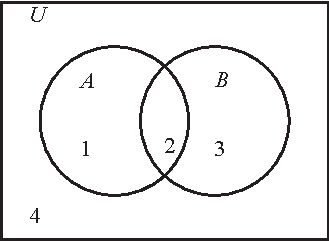
\includegraphics[width=\linewidth]{external/figps-venn2.pdf}
\end{image}%
\tcblower
\end{figureptx}%
In \hyperref[x:figure:fig_venn2-prev]{Figure~{\xreffont\ref{x:figure:fig_venn2-prev}}, p.\,\pageref{x:figure:fig_venn2-prev}}, the elements of \(A\) are represented by the points inside the left circle, and the elements of \(B\) are represented by the points inside the right circle. The four distinct regions in the diagram are numbered for reference purposes only. (The numbers do not represent elements in a set.) The following table describes the four regions in the diagram. \begin{center}%
{\tabularfont%
\begin{tabular}{ccc}
\textbf{Region}&\textbf{Elements of \(U\)}&\textbf{Set}\tabularnewline\hrulemedium
1&In \(A\) and not in \(B\)&\(A - B\)\tabularnewline[0pt]
2&In \(A\) and in \(B\)&\(A \cap B\)\tabularnewline[0pt]
3&In \(B\) and not in \(A\)&\(B - A\)\tabularnewline[0pt]
4&Not in \(A\) and not in \(B\)&\(A^c \cap B^c\)
\end{tabular}
}%
\end{center}%
 We can use these regions to represent other sets. For example, the set \(A \cup B\) is represented by regions 1, 2, and 3 or the shaded region in \hyperref[x:figure:fig_union2]{Figure~{\xreffont\ref{x:figure:fig_union2}}, p.\,\pageref{x:figure:fig_union2}}. \begin{figureptx}{Venn Diagram for \(A \cup B\)}{x:figure:fig_union2}{}%
\begin{image}{0.275}{0.45}{0.275}%
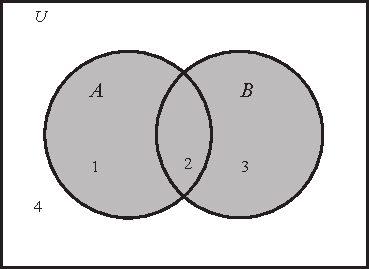
\includegraphics[width=\linewidth]{external/figps-aunionb.pdf}
\end{image}%
\tcblower
\end{figureptx}%
%
\par
Let \(A\) and \(B\) be subsets of a universal set \(U\). For each of the following, draw a Venn diagram for two sets and shade the region that represent the specified set. In addition, describe the set using set builder notation.%
\begin{divisionexercise}{1}{}{}{g:exercise:idm823851432}%
\(A^c\)%
\end{divisionexercise}%
\begin{divisionexercise}{2}{}{}{g:exercise:idm823842600}%
\(B^c\)%
\end{divisionexercise}%
\begin{divisionexercise}{3}{}{}{g:exercise:idm823839016}%
\(A^c \cup B\)%
\end{divisionexercise}%
\begin{divisionexercise}{4}{}{}{g:exercise:idm823839144}%
\(A^c \cup B^c\)%
\end{divisionexercise}%
\begin{divisionexercise}{5}{}{}{g:exercise:idm823842088}%
\(\left( A \cap B \right)^c\)%
\end{divisionexercise}%
\begin{divisionexercise}{6}{}{}{g:exercise:idm823845288}%
\(\left( A \cup B \right) - \left( A \cap B \right)\)%
\end{divisionexercise}%
\end{worksheet-subsection}
%
%
\typeout{************************************************}
\typeout{Subsection  Set Equality, Subsets, and Proper Subsets}
\typeout{************************************************}
%
\begin{subsectionptx}{Set Equality, Subsets, and Proper Subsets}{}{Set Equality, Subsets, and Proper Subsets}{}{}{x:subsection:SS_propersubset}
\label{g:notation:idm823846312}%
In \hyperref[x:section:S_2predicates]{Section~{\xreffont\ref{x:section:S_2predicates}}, p.\,\pageref{x:section:S_2predicates}}, we introduced some basic definitions used in set theory, what it means to say that two sets are equal and what it means to say that one set is a subset of another set. See \hyperref[x:assemblage:D_setequality]{Definition, p.\,\pageref{x:assemblage:D_setequality}}. We need one more definition.%
\begin{assemblage}{Definition.}{x:assemblage:propersubset}%
\label{g:notation:idm823831592} Let \(A\) and \(B\) be two sets contained in some universal set \(U\). The set \(A\) is a \terminology{proper subset} of \(B\) provided that \(A \subseteq B\) and \(A \ne B\). When \(A\) is a proper subset of \(B\), we write \(A \subset B\).%
\end{assemblage}
One reason for the definition of proper subset is that each set is a subset of itself. That is, If \(A\) is a set, then \(A \subseteq A\). However, sometimes we need to indicate that a set \(X\) is a subset of \(Y\) but \(X \ne Y\). For example, if%
\begin{equation*}
X = \left\{ {1, 2} \right\}\text{  and  } Y = \left\{ {0, 1, 2, 3} \right\}\!\text{,}
\end{equation*}
then \(X \subset Y\). We know that \(X \subseteq Y\) since each element of \(X\) is an element of \(Y\), but \(X \ne Y\) since \(0 \in Y\) and \(0 \notin X\). (Also, \(3 \in Y\) and \(3 \notin X\).) Notice that the notations \(A \subset B\) and \(A \subseteq B\) are used in a manner similar to inequality notation for numbers (\(a \lt  b\) and \(a \leq b\)).%
\par
It is often very important to be able to describe precisely what it means to say that one set is not a subset of the other. In the preceding example, \(Y\) is not a subset of \(X\) since there exists an element of \(Y\) (namely, 0) that is not in \(X\).%
\par
In general, the subset relation is described with the use of a universal quantifier since \(A \subseteq B\) means that for each element \(x\) of \(U\), if \(x \in A\), then \(x \in B\). So when we negate this, we use an existential quantifier as follows:%
\begin{align*}
A \subseteq B \amp \amp \text{ means } \amp \amp 
\left( {\forall x \in U} \right)\left[ {\left( {x \in A} \right) \to 
\left( {x \in B} \right)} \right]\\
A \not\subseteq B \amp \amp \text{ means } \amp \amp 
\mynot  \left( {\forall x \in U} \right)\left[ {\left( {x \in A} \right) \to 
\left( {x \in B} \right)} \right]\\
\amp \amp \amp \amp \left( {\exists x \in U} \right) \mynot  
\left[ {\left( {x \in A} \right) \to \left( {x \in B} \right)} \right]\\
\amp \amp \amp \amp \left( {\exists x \in U} \right)
\left[ {\left( {x \in A} \right) \wedge \left( {x \notin B} \right)} \right]\text{.}
\end{align*}
So we see that \(A \not\subseteq B\) means that there exists an \(x\) in \(U\) such that \(x \in A\) and \(x \notin B\).%
\par
Notice that if \(A = \emptyset\), then the conditional statement, ``For each \(x \in U\), if \(x \in \emptyset\), then \(x \in B\)'' must be true since the hypothesis will always be false. Another way to look at this is to consider the following statement: \begin{quote}%
\(\emptyset \not \subseteq B\) means that there exists an \(x \in \emptyset\) such that \(x \notin B\).\end{quote}
 However, this statement must be false since there does not exist an \(x\) in \(\emptyset\). Since this is false, we must conclude that \(\emptyset \subseteq B\). Although the facts that \(\emptyset \subseteq B\) and \(B \subseteq B\) may not seem very important, we will use these facts later, and hence we summarize them in \hyperref[x:theorem:T_subsets]{Theorem~{\xreffont\ref{x:theorem:T_subsets}}, p.\,\pageref{x:theorem:T_subsets}}.%
\begin{theorem}{}{}{x:theorem:T_subsets}%
For any set \(B\), \(\emptyset \subseteq B\) and \(B \subseteq B\).%
\end{theorem}
In \hyperref[x:section:S_2predicates]{Section~{\xreffont\ref{x:section:S_2predicates}}, p.\,\pageref{x:section:S_2predicates}}, we also defined two sets to be equal when they have precisely the same elements. For example,%
\begin{equation*}
\left\{ {\left. {x \in \mathbb{R}\,} \right|\;x^2  = 4} \right\} = 
\left\{ { - 2,\;2} \right\}\!\text{.}
\end{equation*}
%
\par
If the two sets \(A\) and \(B\) are equal, then it must be true that every element of \(A\) is an element of \(B\), that is, \(A \subseteq B\), and it must be true that every element of \(B\) is an element of \(A\), that is, \(B \subseteq A\). Conversely, if \(A \subseteq B\) and \(B \subseteq A\), then \(A\) and \(B\) must have precisely the same elements. This gives us the following test for set equality:%
\begin{theorem}{}{}{x:theorem:T_setequality}%
Let \(A\) and \(B\) be subsets of some universal set \(U\). Then \(A = B\) if and only if \(A \subseteq B\) and \(B \subseteq A\).%
\end{theorem}
\begin{inlineexercise}{Using Set Notation.}{x:exercise:prog_setnotation}%
Let the universal set be \(U = \left\{ {1,2,3,4,5,6} \right\}\), and let%
\begin{equation*}
A = \left\{ {1,2,4} \right\}\!,   B = \left\{ {1,2,3,5} \right\}\!, 
C = \left\{ {\left. {x \in U} \right|x^2  \leq 2} \right\}\!\text{.}
\end{equation*}
%
\par
In each of the following, fill in the blank with one or more of the symbols \(\subset, \\ \subseteq, =, \ne, \in ,\text{ or } \notin\) so that the resulting statement is true. For each blank, include all symbols that result in a true statement. If none of these symbols makes a true statement, write nothing in the blank.%
\begin{enumerate}[font=\bfseries,label=(\alph*),ref=\alph*]
\item{}\(A\)\fillin{4.545454545454546}\(B\)%
\space\hyperlink{g:solution:idm823792680-back}{[Solution]}\item{}5\fillin{4.545454545454546}\(B\)%
\space\hyperlink{g:solution:idm823791144-back}{[Solution]}\item{}\(A\)\fillin{4.545454545454546}\(C\)%
\space\hyperlink{g:solution:idm823793448-back}{[Solution]}\item{}\(\left\{ {1, 2} \right\}\)\fillin{4.545454545454546}\(A\)%
\space\hyperlink{g:solution:idm823797288-back}{[Solution]}\item{}6\fillin{4.545454545454546}\(A\)%
\space\hyperlink{g:solution:idm823783464-back}{[Solution]}\item{}\(\emptyset\)\fillin{4.545454545454546}\(A\)%
\space\hyperlink{g:solution:idm823787560-back}{[Solution]}\item{}\(\left\{ 5 \right\}\)\fillin{4.545454545454546}\(B\)%
\space\hyperlink{g:solution:idm823782568-back}{[Solution]}\item{}\(\left\{ {1, 2} \right\}\)\fillin{4.545454545454546}\(C\)%
\space\hyperlink{g:solution:idm823782056-back}{[Solution]}\item{}\(\left\{ {4, 2, 1} \right\}\)\fillin{4.545454545454546}\(A\)%
\space\hyperlink{g:solution:idm823775400-back}{[Solution]}\item{}\(B\)\fillin{4.545454545454546}\(\emptyset\)%
\space\hyperlink{g:solution:idm823777960-back}{[Solution]}\end{enumerate}
\end{inlineexercise}%
\end{subsectionptx}
%
%
\typeout{************************************************}
\typeout{Subsection  More about Venn Diagrams}
\typeout{************************************************}
%
\begin{subsectionptx}{More about Venn Diagrams}{}{More about Venn Diagrams}{}{}{x:subsection:SS_venn3}
In \hyperref[x:worksheet:PA_venn]{Beginning Activity 2, p.\,\pageref{x:worksheet:PA_venn}}, we learned how to use Venn diagrams as a visual representation for sets, set operations, and set relationships. In that activity, we restricted ourselves to using two sets. We can, of course, include more than two sets in a Venn diagram. \hyperref[x:figure:fig_aintersectc]{Figure~{\xreffont\ref{x:figure:fig_aintersectc}}, p.\,\pageref{x:figure:fig_aintersectc}} shows a general Venn diagram for three sets (including a shaded region that corresponds to \(A \cap C\)).%
\par
In this diagram, there are eight distinct regions, and each region has a unique reference number. For example, the set \(A\) is represented by the combination of regions 1, 2, 4, and 5, whereas the set \(C\) is represented by the combination of regions 4, 5, 6, and 7. This means that the set \(A \cap C\) is represented by the combination of regions 4 and 5. This is shown as the shaded region in \hyperref[x:figure:fig_aintersectc]{Figure~{\xreffont\ref{x:figure:fig_aintersectc}}, p.\,\pageref{x:figure:fig_aintersectc}}.%
\begin{figureptx}{Venn Diagram for \(A \cap C\)}{x:figure:fig_aintersectc}{}%
\begin{image}{0.275}{0.45}{0.275}%
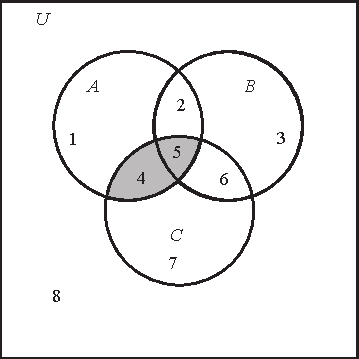
\includegraphics[width=\linewidth]{external/figps-ainterc3.pdf}
\end{image}%
\tcblower
\end{figureptx}%
Finally, Venn diagrams can also be used to illustrate special relationships between sets. For example, if \(A \subseteq B\), then the circle representing \(A\) should be completely contained in the circle for \(B\). So if \(A \subseteq B\), and we know nothing about any relationship between the set \(C\) and the sets \(A\) and \(B\), we could use the Venn diagram shown in \hyperref[x:figure:fig_asubsetb]{Figure~{\xreffont\ref{x:figure:fig_asubsetb}}, p.\,\pageref{x:figure:fig_asubsetb}}.%
\begin{figureptx}{Venn Diagram Showing \(A \subseteq B\)}{x:figure:fig_asubsetb}{}%
\begin{image}{0.275}{0.45}{0.275}%
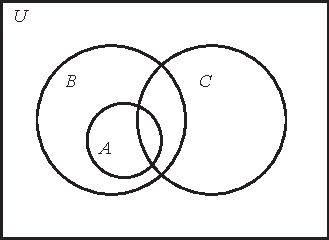
\includegraphics[width=\linewidth]{external/figps-asubsetb3.pdf}
\end{image}%
\tcblower
\end{figureptx}%
\begin{inlineexercise}{Using Venn Diagrams.}{x:exercise:prog_venndiagrams}%
Let \(A\), \(B\), and \(C\) be subsets of a universal set \(U\).%
\begin{enumerate}[font=\bfseries,label=(\alph*),ref=\alph*]
\item{}For each of the following, draw a Venn diagram for three sets and shade the region(s) that represent the specified set.%
\begin{enumerate}[font=\bfseries,label=(\roman*),ref=\theenumi.\roman*]
\item{}\((A \cap B) \cap C\)%
\space\hyperlink{g:solution:idm823764392-back}{[Solution]}\item{}\((A \cap B) \cup C\)%
\space\hyperlink{g:solution:idm823762728-back}{[Solution]}\item{}\(\left( A^c \cup B \right)\)%
\space\hyperlink{g:solution:idm823760168-back}{[Solution]}\item{}\(A^c \cap (B \cup C)\)%
\space\hyperlink{g:solution:idm823751592-back}{[Solution]}\end{enumerate}
\item{}Draw the most general Venn diagram showing \(B \subseteq (A \cup C)\).%
\space\hyperlink{g:solution:idm823754280-back}{[Solution]}\item{}Draw the most general Venn diagram showing \(A \subseteq \left( B^c \cup C \right)\).%
\space\hyperlink{g:solution:idm823756072-back}{[Solution]}\end{enumerate}
\end{inlineexercise}%
\end{subsectionptx}
%
%
\typeout{************************************************}
\typeout{Subsection  The Power Set of a Set}
\typeout{************************************************}
%
\begin{subsectionptx}{The Power Set of a Set}{}{The Power Set of a Set}{}{}{g:subsection:idm823751848}
The symbol \(\in\) is used to describe a relationship between an element of the universal set and a subset of the universal set, and the symbol \(\subseteq\) is used to describe a relationship between two subsets of the universal set. For example, the number 5 is an integer, and so it is appropriate to write \(5 \in \mathbb{Z}\). It is not appropriate, however, to write \(5 \subseteq \mathbb{Z}\) since 5 is not a set. It is important to distinguish between 5 and \(\left\{ 5 \right\}\). The difference is that 5 is an integer and \(\left\{ 5 \right\}\) is a set consisting of one element. Consequently, it is appropriate to write \(\left\{ 5 \right\} \subseteq \mathbb{Z}\), but it is not appropriate to write \(\left\{ 5 \right\} \in \mathbb{Z}\). The distinction between these two symbols \(\left( 5 \text{ and } \left\{ 5 \right\} \right)\) is important when we discuss what is called the power set of a given set.%
\begin{assemblage}{Definition.}{x:assemblage:D_powerset}%
\label{g:notation:idm823741864} If \(A\) is a subset of a universal set \(U\), then the set whose members are all the subsets of \(A\) is called the \terminology{power set} of \(A\). We denote the power set of \(A\) by \(\mathcal{P}( A )\) . Symbolically, we write%
\begin{equation*}
\mathcal{P}( A ) = \left\{ {X \subseteq U  \mid X \subseteq A} \right\}\text{.}
\end{equation*}
That is, \(X \in \mathcal{P}( A )\) if and only if \(X \subseteq A\).%
\end{assemblage}
When dealing with the power set of \(A\), we must always remember that \(\emptyset  \subseteq A\) and \(A \subseteq A\). For example, if \(A = \left\{ {a,b} \right\}\), then the subsets of \(A\) are%
\begin{equation}
\emptyset,\left\{ a \right\}\!,\left\{ b \right\}\!,\left\{ {a,b} \right\}\!\text{.}\label{x:men:eq_subsets2}
\end{equation}
%
\par
We can write this as%
\begin{equation*}
\mathcal{P}( A ) = \left\{ {\emptyset,\left\{ a \right\}\!,\left\{ b \right\}\!,
\left\{ {a,b} \right\}} \right\}\!\text{.}
\end{equation*}
Now let \(B = \left\{ {a, b, c} \right\}\). Notice that \(B = A \cup \{ c \}\). We can determine the subsets of \(B\) by starting with the subsets of \(A\) in \hyperref[x:men:eq_subsets2]{({\xreffont\ref{x:men:eq_subsets2}})}. We can form the other subsets of \(B\) by taking the union of each set in \hyperref[x:men:eq_subsets2]{({\xreffont\ref{x:men:eq_subsets2}})} with the set \(\{c \}\). This gives us the following subsets of \(B\).%
\begin{equation}
\{ c \},\left\{ a, c \right\}\!,\left\{ b, c \right\}\!,\left\{ {a,b, c} \right\}\!\text{.}\label{x:men:eq_subsets2a}
\end{equation}
So the subsets of \(B\) are those sets in \hyperref[x:men:eq_subsets2]{({\xreffont\ref{x:men:eq_subsets2}})} combined with those sets in \hyperref[x:men:eq_subsets2a]{({\xreffont\ref{x:men:eq_subsets2a}})}. That is, the subsets of \(B\) are%
\begin{equation}
\emptyset,\left\{ a \right\}\!,\left\{ b \right\}\!,\left\{ {a,b} \right\}, \{ c \},
\left\{ a, c \right\}\!,\left\{ b, c \right\}\!,\left\{ {a,b, c} \right\}\!\text{,}\label{x:men:eq_subsets2b}
\end{equation}
which means that%
\begin{equation*}
\mathcal{P}( B ) = \left\{ {\emptyset,\left\{ a \right\}\!, \left\{ b \right\}\!, 
\left\{ {a, b} \right\}\!,\left\{ c \right\}\!,\left\{ {a,c} \right\}\!,\left\{ {b,c} 
\right\}\!,\left\{ {a,b,c} \right\}} \right\}\!\text{.}
\end{equation*}
%
\par
Notice that we could write%
\begin{equation*}
\left\{ {a,c} \right\} \subseteq B \text{  or that  } \left\{ {a,c} \right\} \in 
\mathcal{P}( B )\text{.}
\end{equation*}
%
\par
Also, notice that \(A\) has two elements and \(A\) has four subsets, and \(B\) has three elements and \(B\) has eight subsets. Now, let \(n\) be a nonnegative integer. The following result can be proved using mathematical induction. (See \hyperref[x:activity:exer_powerset]{Activity~{\xreffont\ref{x:activity:exer_powerset}}, p.\,\pageref{x:activity:exer_powerset}}.)%
\begin{theorem}{}{}{x:theorem:T_powerset}%
Let \(n\) be a nonnegative integer and let \(T\) be a subset of some universal set. If the set \(T\) has \(n\) elements, then the set \(T\) has \(2^n\) subsets. That is, \(\mathcal{P}(T)\) has \(2^n\) elements.%
\end{theorem}
\end{subsectionptx}
%
%
\typeout{************************************************}
\typeout{Subsection  The Cardinality of a Finite Set}
\typeout{************************************************}
%
\begin{subsectionptx}{The Cardinality of a Finite Set}{}{The Cardinality of a Finite Set}{}{}{g:subsection:idm823718312}
In our discussion of the power set, we were concerned with the number of elements in a set. In fact, the number of elements in a finite set is a distinguishing characteristic of the set, so we give it the following name. \begin{assemblage}{Definition.}{x:assemblage:D_cardinality}%
\label{g:notation:idm823723176} The number of elements in a finite set \(A\) is called the \terminology{cardinality} of \(A\) and is denoted by \(\card(A)\).%
\end{assemblage}
 For example, \(\card (\emptyset) = 0\); \(\card (\left\{ {a,b} \right\}) = 2\); \(\card \left( \mathcal{P}( \left\{ {a,b} \right\}) \right) = 4\).%
\begin{paragraphs}{Theoretical Note.}{g:paragraphs:idm823717544}%
There is a mathematical way to distinguish between finite and infinite sets, and there is a way to define the cardinality of an infinite set. We will not concern ourselves with this at this time.  More about the cardinality of finite and infinite sets is discussed in \hyperref[x:chapter:C_topicsinsets]{Chapter~{\xreffont\ref{x:chapter:C_topicsinsets}}, p.\,\pageref{x:chapter:C_topicsinsets}}.%
\end{paragraphs}%
\end{subsectionptx}
%
%
\typeout{************************************************}
\typeout{Subsection  Standard Number Systems}
\typeout{************************************************}
%
\begin{subsectionptx}{Standard Number Systems}{}{Standard Number Systems}{}{}{g:subsection:idm823712936}
\index{natural numbers}%
\index{integers}%
We can use set notation to specify and help describe our standard number systems. The starting point is the set of \terminology{natural numbers}, for which we use the roster method.%
\begin{equation*}
\N = \left\{ 1, 2, 3, 4, \ldots \;\right\}
\end{equation*}
%
\par
The \terminology{integers} consist of the natural numbers, the negatives of the natural numbers, and zero. If we let \(\N^- = \left\{ \ldots, -4, -3, -2, -1 \right\}\), then we can use set union and write%
\begin{equation*}
\Z = \N^- \cup \left\{ 0 \right\} \cup \N\text{.}
\end{equation*}
So we see that \(\N \subseteq \Z\), and in fact, \(\N \subset \Z\).%
\par
We need to use set builder notation for the set \(\Q\) of all \terminology{rational numbers}, which consists of quotients of integers.%
\begin{equation*}
\Q = \left\{ \left. \frac{m}{n}  \right| m, n \in \Z \text{ and }  n \ne 0 \right\}
\end{equation*}
Since any integer \(n\) can be written as \(n = \dfrac{n}{1}\), we see that \(\Z \subseteq \Q\).%
\par
\index{real numbers}\index{irrational numbers} We do not yet have the tools to give a complete description of the real numbers. We will simply say that the \terminology{real numbers} consist of the rational numbers and the \terminology{irrational numbers}. In effect, the irrational numbers are the complement of the set of rational numbers \(\Q\) in \(\R\). So we can use the notation \(\Q^c = \left\{ x \in \R \mid x \notin \Q \right\}\) and write%
\begin{equation*}
\R = \Q \cup \Q^c \qquad \text{ and }  \qquad \Q \cap \Q^c = \emptyset\text{.}
\end{equation*}
%
\par
\index{complex numbers} A number system that we have not yet discussed is the set of \terminology{complex numbers}. The complex numbers, \(\mathbb{C}\), consist of all numbers of the form \(a + bi\), where \(a,
b \in \R\) and \(i = \sqrt{-1}\) (or \(i^2 = -1\)). That is,%
\begin{equation*}
\mathbb{C} = \left\{  a + bi \left|  a, b \in \R \text{ and }  i = \sqrt{-1} \right. \right\}\!\text{.}
\end{equation*}
We can add and multiply complex numbers as follows: If \(a,
b, c, d \in \R\), then%
\begin{align*}
\left( a + bi \right) + \left( c + di \right) \amp 
= \left(a + c \right) + \left(b + d \right)i, \text{ and }\\
\left( a + bi \right) \left( c + di \right) \amp = ac + adi + bci + bdi^2\\
\amp = \left(ac - bd \right) + \left(ad + bc \right)i\text{.}
\end{align*}
%
\end{subsectionptx}
%
%
\typeout{************************************************}
\typeout{Exercises  Exercises}
\typeout{************************************************}
%
\begin{exercises-subsection}{Exercises}{}{Exercises}{}{}{g:exercises:idm823694376}
\begin{divisionexercise}{1}{}{}{x:exercise:exer_sec41-1}%
Assume the universal set is the set of real numbers. Let%
\begin{align*}
A \amp = \left\{ { - 3, - 2,2,3} \right\}\!, \amp   B \amp 
= \left\{ {\left. {x \in \mathbb{R}} \right|x^2  = 4\text{  or  } x^2  = 9} \right\}\!,\\
C \amp = \left\{ {x \in \mathbb{R}\left.  \right|x^2  + 2 = 0} \right\}\!,  
\amp  D \amp = \left\{ {x \in \mathbb{R}\left.  \right|x > 0} \right\}\!\text{.}
\end{align*}
Respond to each of the following questions. In each case, explain your answer.%
\begin{enumerate}[font=\bfseries,label=(\alph*),ref=\alph*]
\item{}Is the set \(A\) equal to the set \(B\)?%
\space\hyperlink{g:answer:idm823691048-back}{[Answer]}\item{}Is the set \(A\) a subset of the set \(B\)?%
\space\hyperlink{g:answer:idm823692712-back}{[Answer]}\item{}Is the set \(C\) equal to the set \(D\)?%
\space\hyperlink{g:answer:idm823691816-back}{[Answer]}\item{}Is the set \(C\) a subset of the set \(D\)?%
\space\hyperlink{g:answer:idm823690280-back}{[Answer]}\item{}Is the set \(A\) a subset of the set \(D\)?%
\space\hyperlink{g:answer:idm823684392-back}{[Answer]}\end{enumerate}
\end{divisionexercise}%
\begin{divisionexercise}{2}{}{}{x:exercise:exer41-equalsets}%
Explain why%
\begin{enumerate}[font=\bfseries,label=(\alph*),ref=\alph*]
\item{}the set \(\left\{ {a,b} \right\}\) is equal to the set \(\left\{ {b,a} \right\}\).%
\space\hyperlink{g:answer:idm823689640-back}{[Answer]}\item{}the set \(\left\{ {a,b,b,a,c} \right\}\) is equal to the set \(\left\{ {b,c,a} \right\}\).%
\space\hyperlink{g:answer:idm823685672-back}{[Answer]}\end{enumerate}
\end{divisionexercise}%
\begin{divisionexercise}{3}{}{}{x:exercise:exer_sec41-3}%
Assume that the universal set is the set of integers. Let%
\begin{align*}
A \amp = \left\{ { - 3, - 2,2,3} \right\}\!,  \amp   B 
\amp = \left\{ {x \in \mathbb{Z}\left.  \right|x^2  \leq 9} \right\}\!,\\
C \amp = \left\{ {\left. {x \in \mathbb{Z}} \right|x \geq  - 3} \right\}\!,  
\amp   D \amp = \left\{ {1,2,3,4} \right\}\!\text{.}
\end{align*}
In each of the following, fill in the blank with one or more of the symbols  \(\subset\) , \(\subseteq\) , \(\not \subseteq\), \(=\) , \(\ne\), \(\in\), \(\text{ or }  \notin\) so that the resulting statement is true. For each blank, include all symbols that result in a true statement. If none of these symbols makes a true statement, write nothing in the blank.%
\begin{enumerate}[font=\bfseries,label=(\alph*),ref=\alph*]
\item{}\(A\)\fillin{4.545454545454546}\(B\)%
\space\hyperlink{g:answer:idm823585576-back}{[Answer]}\item{}5\fillin{4.545454545454546}\(C\)%
\space\hyperlink{g:answer:idm823592104-back}{[Answer]}\item{}\(A\)\fillin{4.545454545454546}\(C\)%
\space\hyperlink{g:answer:idm823591720-back}{[Answer]}\item{}\(\left\{ 1, 2 \right\}\)\fillin{4.545454545454546}\(A\)%
\space\hyperlink{g:answer:idm823587880-back}{[Answer]}\item{}4\fillin{4.545454545454546}\(B\)%
\space\hyperlink{g:answer:idm823579688-back}{[Answer]}\item{}\(\card(A)\)\fillin{4.545454545454546}\(\card(D)\)%
\space\hyperlink{g:answer:idm823581736-back}{[Answer]}\item{}\(A\)\fillin{4.545454545454546}\(\mathcal{P}(A)\)%
\space\hyperlink{g:answer:idm823578664-back}{[Answer]}\item{}\(\emptyset\)\fillin{4.545454545454546}\(A\)%
\space\hyperlink{g:answer:idm823582120-back}{[Answer]}\item{}\(\left\{ 5 \right\}\)\fillin{4.545454545454546}\(C\)%
\space\hyperlink{g:answer:idm823568808-back}{[Answer]}\item{}\(\left\{ 1, 2 \right\}\)\fillin{4.545454545454546}\(B\)%
\space\hyperlink{g:answer:idm823569320-back}{[Answer]}\item{}\(\left\{ 3, 2, 1 \right\}\)\fillin{4.545454545454546}\(D\)%
\space\hyperlink{g:answer:idm823571496-back}{[Answer]}\item{}\(D\)\fillin{4.545454545454546}\(\emptyset\)%
\space\hyperlink{g:answer:idm823575080-back}{[Answer]}\item{}\(\card(A)\)\fillin{4.545454545454546}\(\card(B)\)%
\space\hyperlink{g:answer:idm823564712-back}{[Answer]}\item{}\(A\)\fillin{4.545454545454546}\(\mathcal{P}(B)\)%
\space\hyperlink{g:answer:idm823562920-back}{[Answer]}\end{enumerate}
\end{divisionexercise}%
\begin{divisionexercise}{4}{}{}{x:exercise:exer_sec51-numbers}%
Write all of the proper subset relations that are possible using the sets of numbers \(\mathbb{N}\), \(\mathbb{Z}\), \(\mathbb{Q}\), and \(\mathbb{R}\).%
\space\hyperlink{g:answer:idm823561128-back}{[Answer]}\end{divisionexercise}%
\begin{divisionexercise}{5}{}{}{x:exercise:exer_sec41-5}%
For each statement, write a brief, clear explanation of why the statement is true or why it is false.%
\begin{enumerate}[font=\bfseries,label=(\alph*),ref=\alph*]
\item{}The set \(\left\{ {a,b} \right\}\) is a subset of \(\left\{ {a,c,d,e} \right\}\).%
\space\hyperlink{g:answer:idm823553064-back}{[Answer]}\item{}The set \(\left\{ { - 2,0,2} \right\}\) is equal to \(\left\{ {x \in \mathbb{Z} \mid x\text{ is even and } x^2 \lt 5} \right\}\).%
\space\hyperlink{g:answer:idm823553960-back}{[Answer]}\item{}The empty set \(\emptyset\) is a subset of \(\left\{ 1 \right\}\).%
\space\hyperlink{g:answer:idm823557288-back}{[Answer]}\item{}If \(A = \left\{ {a,b} \right\}\), then the set \(\left\{ a \right\}\) is a subset of \(\mathcal{P}( A )\).%
\space\hyperlink{g:answer:idm823549224-back}{[Answer]}\end{enumerate}
\end{divisionexercise}%
\begin{divisionexercise}{6}{}{}{x:exercise:exer_sec41-8}%
Use the definitions of set intersection, set union, and set difference to write useful negations of these definitions. That is, complete each of the following sentences%
\begin{enumerate}[font=\bfseries,label=(\alph*),ref=\alph*]
\item{}\(x \notin A \cap B\) if and only if \(\ldots \).%
\space\hyperlink{g:answer:idm823544232-back}{[Answer]}\item{}\(x \notin A \cup B\) if and only if \(\ldots \).%
\item{}\(x \notin A - B\) if and only if \(\ldots \).%
\end{enumerate}
\end{divisionexercise}%
\begin{divisionexercise}{7}{}{}{x:exercise:exer_sec41-6}%
Let \(U = \left\{ {1,2,3,4,5,6,7,8,9,10} \right\}\), and let%
\begin{align*}
A \amp = \left\{ {3,4,5,6,7} \right\}\!,  \amp   
B \amp = \left\{ {1,5,7,9} \right\}\!,\\
C \amp = \left\{ {3,6,9} \right\}\!,      \amp   
D \amp = \left\{ {2,4,6,8} \right\}\!\text{.}
\end{align*}
Use the roster method to list all of the elements of each of the following sets.%
\begin{enumerate}[font=\bfseries,label=(\alph*),ref=\alph*]
\item{}\(A \cap B\)%
\space\hyperlink{g:answer:idm823539752-back}{[Answer]}\item{}\(A \cup B\)%
\space\hyperlink{g:answer:idm823539496-back}{[Answer]}\item{}\(\left( {A \cup B} \right)^c\)%
\space\hyperlink{g:answer:idm823542824-back}{[Answer]}\item{}\(A^c \cap B^c\)%
\space\hyperlink{g:answer:idm823541672-back}{[Answer]}\item{}\(\left( {A \cup B} \right) \cap C\)%
\space\hyperlink{g:answer:idm823530408-back}{[Answer]}\item{}\(A \cap C\)%
\space\hyperlink{g:answer:idm823533864-back}{[Answer]}\item{}\(B \cap C\)%
\space\hyperlink{g:answer:idm823535272-back}{[Answer]}\item{}\(\left( {A \cap C} \right) \cup \left( {B \cap C} \right)\)%
\space\hyperlink{g:answer:idm823530152-back}{[Answer]}\item{}\(B \cap D\)%
\space\hyperlink{g:answer:idm823529000-back}{[Answer]}\item{}\(\left( {B \cap D} \right)^c\)%
\space\hyperlink{g:answer:idm823525160-back}{[Answer]}\item{}\(A - D\)%
\space\hyperlink{g:answer:idm823519528-back}{[Answer]}\item{}\(B - D\)%
\space\hyperlink{g:answer:idm823523240-back}{[Answer]}\item{}\(\left( A - D \right) \cup \left( B - D \right)\)%
\space\hyperlink{g:answer:idm823524520-back}{[Answer]}\item{}\(\left( A \cup B \right) - D\)%
\space\hyperlink{g:answer:idm823519656-back}{[Answer]}\end{enumerate}
\end{divisionexercise}%
\begin{divisionexercise}{8}{}{}{x:exercise:exer_sec41-6x}%
Let  \(U = \N\), and let%
\begin{align*}
A \amp = \left\{ x \in \N \mid x \geq 7 \right\}\!,  \amp   
B \amp = \left\{ x \in \N \mid x \text{ is odd }  \right\}\!,\\
C \amp = \left\{ x \in \N \mid x \text{ is a multiple of 3 }  \right\}\!, 
\amp D \amp = \left\{ x \in \N \mid x \text{ is even }  \right\}\!\text{.}
\end{align*}
Use the roster method to list all of the elements of each of the following sets.%
\begin{enumerate}[font=\bfseries,label=(\alph*),ref=\alph*]
\item{}\(A \cap B\)%
\item{}\(A \cup B\)%
\item{}\(\left( {A \cup B} \right)^c\)%
\item{}\(A^c \cap B^c\)%
\item{}\(\left( {A \cup B} \right) \cap C\)%
\item{}\(\left( {A \cap C} \right) \cup \left( {B \cap C} \right)\)%
\item{}\(B \cap D\)%
\item{}\(\left( {B \cap D} \right)^c\)%
\item{}\(A - D\)%
\item{}\(B - D\)%
\item{}\(\left( A - D \right) \cup \left( B - D \right)\)%
\item{}\(\left( A \cup B \right) - D\)%
\end{enumerate}
\end{divisionexercise}%
\begin{divisionexercise}{9}{}{}{g:exercise:idm823505192}%
Let \(P\), \(Q\), \(R\), and \(S\) be subsets of a universal set \(U\). Assume that \(\left( P - Q \right) \subseteq \left( R \cap S \right)\).%
\begin{enumerate}[font=\bfseries,label=(\alph*),ref=\alph*]
\item\label{x:task:exer_subset-defa}Complete the following sentence: \begin{quote}%
For each \(x \in U\), if \(x \in \left( P - Q \right)\), then \(\ldots \).\end{quote}
%
\item{}Write a useful negation of the statement in \hyperref[x:task:exer_subset-defa]{Task~{\xreffont 9}.{\xreffont\ref{x:task:exer_subset-defa}}, p.\,\pageref{x:task:exer_subset-defa}}.%
\space\hyperlink{g:answer:idm823494440-back}{[Answer]}\item{}Write the contrapositive of the statement in \hyperref[x:task:exer_subset-defa]{Task~{\xreffont 9}.{\xreffont\ref{x:task:exer_subset-defa}}, p.\,\pageref{x:task:exer_subset-defa}}.%
\end{enumerate}
\end{divisionexercise}%
\begin{divisionexercise}{10}{}{}{x:exercise:exer_sec41-10}%
Let \(U\) be the universal set. Consider the following statement: \begin{quote}%
For all \(A\) and \(B\) that are subsets of \(U\), if \(A \subseteq B\), then \(B^c \subseteq A^c\).\end{quote}
%
\begin{enumerate}[font=\bfseries,label=(\alph*),ref=\alph*]
\item{}Identify three conditional statements in the given statement.%
\space\hyperlink{g:answer:idm823488680-back}{[Answer]}\item{}Write the contrapositive of this statement.%
\item{}Write the negation of this statement.%
\end{enumerate}
\end{divisionexercise}%
\begin{divisionexercise}{11}{}{}{x:exercise:exer_sec41-11}%
Let \(A\), \(B\), and \(C\) be subsets of some universal set \(U\). Draw a Venn diagram for each of the following situations.%
\begin{enumerate}[font=\bfseries,label=(\alph*),ref=\alph*]
\item{}\(A \subseteq C\)%
\item{}\(A \cap B = \emptyset\)%
\item{}\(A \not \subseteq B,B \not \subseteq A,C \subseteq A,\text{ and } C \not \subseteq B\)%
\item{}\(A \subseteq B,C \subseteq B,\text{ and } A \cap C = \emptyset\)%
\end{enumerate}
\end{divisionexercise}%
\begin{divisionexercise}{12}{}{}{x:exercise:exer_sec41-12}%
Let \(A\), \(B\), and \(C\) be subsets of some universal set \(U\). For each of the following, draw a general Venn diagram for the three sets and then shade the indicated region.%
\begin{enumerate}[font=\bfseries,label=(\alph*),ref=\alph*]
\item{}\(A \cap B\)%
\item{}\(A \cap C\)%
\item{}\(\left( {A \cap B} \right) \cup \left( {A \cap C} \right)\)%
\item{}\(B \cup C\)%
\item{}\(A \cap \left( {B \cup C} \right)\)%
\item{}\(\left( {A \cap B} \right) - C\)%
\end{enumerate}
\end{divisionexercise}%
\begin{divisionexercise}{13}{}{}{x:exercise:exer_congruence41}%
We can extend the idea of consecutive integers (See \hyperlink{x:exercise:exer_sec34-2}{Exercise~{\xreffont 10}, p.\,\pageref{x:exercise:exer_sec34-2}} in \hyperref[x:section:S_divalgo]{Section~{\xreffont\ref{x:section:S_divalgo}}, p.\,\pageref{x:section:S_divalgo}}) to represent four consecutive integers as \(m\), \(m + 1\), \(m + 2\), and \(m + 3\), where \(m\) is an integer. There are other ways to represent four consecutive integers. For example, if \(k \in \Z\), then \(k - 1\), \(k\), \(k + 1\), and \(k + 2\) are four consecutive integers.%
\begin{enumerate}[font=\bfseries,label=(\alph*),ref=\alph*]
\item{}Prove that for each \(n \in \Z\), \(n\) is the sum of four consecutive integers if and only if \(n \equiv 2 \pmod 4\).%
\item{}Use set builder notation or the roster method to specify the set of integers that are the sum of four consecutive integers.%
\item{}Specify the set of all natural numbers that can be written as the sum of four consecutive natural numbers.%
\item{}Prove that for each \(n \in \Z\), \(n\) is the sum of eight consecutive integers if and only if \(n \equiv 4 \pmod 8\).%
\item{}Use set builder notation or the roster method to specify the set of integers that are the sum of eight consecutive integers.%
\item{}Specify the set of all natural numbers can be written as the sum of eight consecutive natural numbers.%
\end{enumerate}
\end{divisionexercise}%
\begin{divisionexercise}{14}{}{}{g:exercise:idm823467688}%
\index{Law of Trichotomy}%
One of the properties of real numbers is the so-called \terminology{Law of Trichotomy}, which states that if \(a,
b \in \R\), then exactly one of the following is true:%
\begin{multicols}{3}
\begin{itemize}[label=\textbullet]
\item{}\(a \lt b\);%
\item{}\(a = b\);%
\item{}\(a > b\).%
\end{itemize}
\end{multicols}
Is the following proposition concerning sets true or false? Either provide a proof that it is true or a counterexample showing it is false. If \(A\) and \(B\) are subsets of some universal set, then exactly one of the following is true:%
\begin{multicols}{3}
\begin{itemize}[label=\textbullet]
\item{}\(A \subseteq B\);%
\item{}\(A = B\);%
\item{}\(B \subseteq A\).%
\end{itemize}
\end{multicols}
%
\end{divisionexercise}%
\begin{activity}{Intervals of Real Numbers.}{x:activity:A_intervals}%
\index{open ray}%
\index{ray!open}%
\index{open interval}%
\index{interval!open}%
\index{closed interval}%
\index{interval!closed}%
\index{half-open interval}%
\index{interval!half-open}%
\index{closed ray}%
\index{ray!closed}%
\index{interval}%
In previous mathematics courses, we have frequently used subsets of the real numbers called \terminology{intervals}. There are some common names and notations for intervals. These are given in the following table, where it is assumed that \(a\) and \(b\) are real numbers and \(a \lt b\).%
\begin{center}%
{\tabularfont%
\begin{tabular}{lll}
\tablecelllines{l}{m}
{Interval\\
Notation}
&Set Notation&Name\tabularnewline\hrulemedium
\(\left( {a,b} \right) =\)&\(\left\{ {x \in \mathbb{R}\left. \right|a \lt x \lt b} \right\}\)&Open interval from \(a\) to \(b\)\tabularnewline[0pt]
\(\left[ {a,b} \right] =\)&\(\left\{ {x \in \mathbb{R}\left. \right|a \leq x \leq b} \right\}\)&Closed interval from \(a\) to \(b\)\tabularnewline[0pt]
\(\left[ {a,b} \right) =\)&\(\left\{ {x \in \mathbb{R}\left. \right|a \leq x \lt b} \right\}\)&Half-open interval\tabularnewline[0pt]
\(\left( {a,b} \right] =\)&\(\left\{ {x \in \mathbb{R}\left. \right|a \lt x \leq b} \right\}\)&Half-open interval\tabularnewline[0pt]
\(\left( {a, + \infty } \right) =\)&\(\left\{ {\left. {x \in \mathbb{R}} \right|x > a} \right\}\)&Open ray\tabularnewline[0pt]
\(\left( { - \infty ,b} \right) =\)&\(\left\{ {\left. {x \in \mathbb{R}} \right|x \lt b} \right\}\)&Open ray\tabularnewline[0pt]
\(\left[ {a, + \infty } \right) =\)&\(\left\{ {\left. {x \in \mathbb{R}} \right|x \geq a} \right\}\)&Closed ray\tabularnewline[0pt]
\(\left( { - \infty ,b} \right] =\)&\(\left\{ {\left. {x \in \mathbb{R}} \right|x \leq b} \right\}\)&Closed ray
\end{tabular}
}%
\end{center}%
\begin{enumerate}[font=\bfseries,label=(\alph*),ref=\alph*]
\item{}Is \(\left( {a,b} \right)\) a proper subset of \(\left( {a,b} \right]\)? Explain.%
\item{}Is \(\left[ {a,b} \right]\) a subset of \(\left( {a, + \infty } \right)\)? Explain.%
\item{}Use interval notation to describe%
\begin{enumerate}[font=\bfseries,label=(\roman*),ref=\theenumi.\roman*]
\item{}the intersection of the interval \(\left[ { - 3,7} \right]\) with the interval \(\left( {5,9} \right]\);%
\item{}the union of the interval \(\left[ { - 3,7} \right]\) with the interval \(\left( {5,9} \right]\);%
\item{}the set difference \(\left[ -3, 7 \right] - \left( 5, 9 \right]\).%
\end{enumerate}
\item{}Write the set \(\left\{ {x \in \mathbb{R}} \mid \left| x \right| \leq 0.01 \right\}\) using interval notation.%
\item{}Write the set \(\left\{ x \in \mathbb{R} \mid \left| x \right| > 2 \right\}\) as the union of two intervals.%
\end{enumerate}
\end{activity}%
\begin{activity}{More Work with Intervals.}{x:activity:exer_intervals41}%
For this exercise, use the interval notation described in \hyperref[x:activity:A_intervals]{Activity~{\xreffont\ref{x:activity:A_intervals}}, p.\,\pageref{x:activity:A_intervals}}.%
\begin{enumerate}[font=\bfseries,label=(\alph*),ref=\alph*]
\item{}Determine the intersection and union of \([2, 5]\) and \([-1, +\infty)\).%
\item{}Determine the intersection and union of \([2, 5]\) and \([3.4, +\infty)\).%
\item{}Determine the intersection and union of \([2, 5]\) and \([7, +\infty)\).%
\item{}Now let \(a\), \(b\), and \(c\) be real numbers with \(a \lt b\).%
\par
Explain why the intersection of \([a, b]\) and \([c, +\infty)\) is either a closed interval, a set with one element, or the empty set.%
\item{}Explain why the union of \([a, b]\) and \([c, +\infty)\) is either a closed ray or the union of a closed interval and a closed ray.%
\end{enumerate}
\end{activity}%
\begin{activity}{Proof of Theorem~{\xreffont\ref*{x:theorem:T_powerset}}.}{x:activity:exer_powerset}%
\index{power set}%
\index{power set!cardinality}%
To help with the proof by induction of \hyperref[x:theorem:T_powerset]{Theorem~{\xreffont\ref{x:theorem:T_powerset}}, p.\,\pageref{x:theorem:T_powerset}}, we first prove the following lemma. (The idea for the proof of this lemma was illustrated with the discussion of power set after \hyperref[x:assemblage:D_powerset]{Definition, p.\,\pageref{x:assemblage:D_powerset}}.) \begin{lemma}{}{}{x:lemma:L_inductivestepforsubsets}%
Let \(A\) and \(B\) be subsets of some universal set. If \(A = B \cup \left\{ x \right\}\), where \(x \notin B\), then any subset of \(A\) is either a subset of \(B\) or a set of the form \(C \cup \left\{ x \right\}\), where \(C\) is a subset of \(B\).%
\end{lemma}
\begin{proof}{}{g:proof:idm823415336}
Let \(A\) and \(B\) be subsets of some universal set, and assume that \(A = B \cup \left\{ x \right\}\) where \(x \notin B\). Let \(Y\) be a subset of \(A\). We need to show that \(Y\) is a subset of \(B\) or that \(Y = C \cup \left\{ x \right\}\), where \(C\) is some subset of \(B\). There are two cases to consider: (1) \(x\) is not an element of \(Y\), and (2) \(x\) is an element of \(Y\).%
\par
Case 1: Assume that \(x \notin Y\). Let \(y \in Y\). Then \(y \in A\) and \(y \ne x\). Since%
\begin{equation*}
A = B \cup \left\{ x \right\}\!\text{,}
\end{equation*}
this means that \(y\) must be in \(B\). Therefore, \(Y \subseteq B\).%
\par
Case 2: Assume that \(x \in Y\). In this case, let \(C = Y - \left\{ x \right\}\). Then every element of \(C\) is an element of \(B\). Hence, we can conclude that \(C \subseteq B\) and that \(Y = C \cup \left\{ x \right\}\).%
\par
Cases (1) and (2) show that if \(Y \subseteq A\), then \(Y \subseteq B\) or \(Y = C \cup \left\{ x \right\}\), where \(C \subseteq B\).%
\end{proof}
%
\par
To begin the induction proof of \hyperref[x:theorem:T_powerset]{Theorem~{\xreffont\ref{x:theorem:T_powerset}}, p.\,\pageref{x:theorem:T_powerset}}, for each nonnegative integer \(n\), we let \(P ( n )\) be, ``If   a finite set has exactly \(n\)  elements, then  that set  has exactly  \(2^n\) subsets.''%
\begin{enumerate}[font=\bfseries,label=(\alph*),ref=\alph*]
\item{}Verify that \(P ( 0 )\) is true. (This is the basis step for the induction proof.)%
\item{}Verify that \(P( 1 )\) and \(P( 2 )\) are true.%
\item{}Now assume that \(k\) is a nonnegative integer and assume that \(P( k )\) is true. That is, assume that if a set has \(k\) elements, then that set has \(2^k\) subsets. (This is the inductive assumption for the induction proof.) Let \(T\) be a subset of the universal set with \(\card (T) = k + 1\), and let \(x \in T\). Then the set \(B = T - \left\{ x \right\}\) has \(k\) elements. Now use the inductive assumption to determine how many subsets \(B\) has. Then use \hyperref[x:lemma:L_inductivestepforsubsets]{Lemma~{\xreffont\ref{x:lemma:L_inductivestepforsubsets}}, p.\,\pageref{x:lemma:L_inductivestepforsubsets}} to prove that \(T\) has twice as many subsets as \(B\). This should help complete the inductive step for the induction proof.%
\end{enumerate}
\end{activity}%
\end{exercises-subsection}
\end{sectionptx}
%
%
\typeout{************************************************}
\typeout{Section 5.2 Proving Set Relationships}
\typeout{************************************************}
%
\begin{sectionptx}{Proving Set Relationships}{}{Proving Set Relationships}{}{}{x:section:S_provingset}
%
%
\typeout{************************************************}
\typeout{Beginning Activity  Beginning Activity 1: Working with Two Specific Sets}
\typeout{************************************************}
%
\begin{worksheet-subsection}{Beginning Activity 1: Working with Two Specific Sets}{}{Beginning Activity 1: Working with Two Specific Sets}{}{}{x:worksheet:PA_working2sets}
Let \(S\) be the set of all integers that are multiples of 6, and let \(T\) be the set of all even integers.%
\begin{divisionexercise}{1}{}{}{g:exercise:idm823383208}%
List at least four different positive elements of \(S\) and at least four different negative elements of \(S\). Are all of these integers even?%
\end{divisionexercise}%
\begin{divisionexercise}{2}{}{}{g:exercise:idm823386152}%
Use the roster method to specify the sets \(S\) and \(T\). (See \hyperref[x:section:S_2predicates]{Section~{\xreffont\ref{x:section:S_2predicates}}, p.\,\pageref{x:section:S_2predicates}} for a review of the roster method.) Does there appear to be any relationship between these two sets? That is, does it appear that the sets are equal or that one set is a subset of the other set?%
\end{divisionexercise}%
\begin{divisionexercise}{3}{}{}{g:exercise:idm823386792}%
Use set builder notation to specify the sets \(S\) and \(T\). (See \hyperref[x:section:S_2predicates]{Section~{\xreffont\ref{x:section:S_2predicates}}, p.\,\pageref{x:section:S_2predicates}} for a review of the set builder notation.)%
\end{divisionexercise}%
\begin{divisionexercise}{4}{}{}{g:exercise:idm823383720}%
Using appropriate definitions, describe what it means to say that an integer \(x\) is a multiple of 6 and what it means to say that an integer \(y\) is even.%
\end{divisionexercise}%
\begin{divisionexercise}{5}{}{}{g:exercise:idm823387688}%
\index{choose-an-element method}%
In order to prove that \(S\) is a subset of \(T\), we need to prove that for each integer \(x\), if \(x \in S\), then \(x \in T\)%
\par
Complete the know-show~table in \hyperref[x:table:table_preview42]{Table~{\xreffont\ref{x:table:table_preview42}}, p.\,\pageref{x:table:table_preview42}} for the proposition that \(S\) is a subset of \(T\).%
\par
This table is in the form of a proof method called the \terminology{choose-an-element method.} This method is frequently used when we encounter a universal quantifier in a statement in the backward process. (In this case, this is Step \(Q1\).) The key is that we have to prove something about all elements in \(\Z\). We can then add something to the forward process by choosing an arbitrary element from the set \(S\). (This is done in Step \(P1\).) This does not mean that we can choose a specific element of \(S\). Rather, we must give the arbitrary element a name and use only the properties it has by being a member of the set \(S\). In this case, the element is a multiple of 6. \begin{tableptx}{\textbf{Know-show table for Beginning Activity 1}}{x:table:table_preview42}{}%
\centering%
{\tabularfont%
\begin{tabular}{lll}
\multicolumn{1}{lB}{Step}&\multicolumn{1}{lB}{Know}&Reason\tabularnewline\hrulemedium
\multicolumn{1}{lB}{\(P\)}&\multicolumn{1}{lB}{\tablecelllines{l}{m}
{\(S\) is the set of all integers that\\
are multiples of 6.\\
\(T\) is the set of all even integers.}
}&Hypothesis\tabularnewline\hrulethin
\multicolumn{1}{lB}{\(P1\)}&\multicolumn{1}{lB}{Let \(x \in S\).}&\tablecelllines{l}{m}
{Choose an arbitrary element\\
of \(S\).}
\tabularnewline\hrulethin
\multicolumn{1}{lB}{\(P2\)}&\multicolumn{1}{lB}{\(\left( {\exists m \in \mathbb{Z}} \right)
\left( {x = 6m} \right)\)}&Definition of ``multiple''\tabularnewline\hrulethin
\multicolumn{1}{lB}{\(\vdots\)}&\multicolumn{1}{lB}{\(\vdots\)}&\(\vdots\)\tabularnewline\hrulethin
\multicolumn{1}{lB}{\(Q2\)}&\multicolumn{1}{lB}{\(x\) is an element of \(T\).}&\(x\) is even\tabularnewline\hrulemedium
\multicolumn{1}{lB}{\(Q1\)}&\multicolumn{1}{lB}{\(\left( \forall x \in \Z \right) \left[ \left( x \in S \right) \to 
\left( x \in T \right) \right]\)}&Step \(P1\) and Step \(Q2\)\tabularnewline\hrulethin
\multicolumn{1}{lB}{\(Q\)}&\multicolumn{1}{lB}{\(S \subseteq T\).}&Definition of ``subset''\tabularnewline\hrulemedium
\multicolumn{1}{lB}{Step}&\multicolumn{1}{lB}{Show}&Reason
\end{tabular}
}%
\end{tableptx}%
%
\end{divisionexercise}%
\end{worksheet-subsection}
%
%
\typeout{************************************************}
\typeout{Beginning Activity  Beginning Activity 2: Working with Venn Diagrams}
\typeout{************************************************}
%
\begin{worksheet-subsection}{Beginning Activity 2: Working with Venn Diagrams}{}{Beginning Activity 2: Working with Venn Diagrams}{}{}{x:worksheet:PA_workingvenn}
\begin{divisionexercise}{1}{}{}{g:exercise:idm823350440}%
Draw a Venn diagram for two sets, \(A\) and \(B\), with the assumption that \(A\) is a subset of \(B\). On this Venn diagram, lightly shade the area corresponding to \(A^c\). Then, determine the region on the Venn diagram that corresponds to \(B^c\). What appears to be the relationship between \(A^c\) and \(B^c\)? Explain.%
\end{divisionexercise}%
\begin{divisionexercise}{2}{}{}{g:exercise:idm823348264}%
Draw a general Venn diagram for two sets, \(A\) and \(B\). First determine the region that corresponds to the set \(A - B\) and then, on the Venn diagram, shade the region corresponding to \(A - (A - B)\) and shade the region corresponding to \(A \cap B\). What appears to be the relationship between these two sets? Explain.%
\end{divisionexercise}%
\end{worksheet-subsection}
\begin{introduction}{}%
In this section, we will learn how to prove certain relationships about sets. Two of the most basic types of relationships between sets are the equality relation and the subset relation. So if we are asked a question of the form, ``How are the sets \(A\) and \(B\) related?'', we can answer the question if we can prove that the two sets are equal or that one set is a subset of the other set. There are other ways to answer this, but we will concentrate on these two for now. This is similar to asking a question about how two real numbers are related. Two real numbers can be related by the fact that they are equal or by the fact that one number is less than the other number.%
\end{introduction}%
%
%
\typeout{************************************************}
\typeout{Subsection  The Choose-an-Element Method}
\typeout{************************************************}
%
\begin{subsectionptx}{The Choose-an-Element Method}{}{The Choose-an-Element Method}{}{}{x:subsection:SS_choosemethod}
\index{choose-an-element method}%
The method of proof we will use in this section can be called the \terminology{choose-an-element method.} This method was introduced in \hyperref[x:worksheet:PA_working2sets]{Beginning Activity 1, p.\,\pageref{x:worksheet:PA_working2sets}}. This method is frequently used when we encounter a universal quantifier in a statement in the backward process. This statement often has the form \begin{quote}%
For each element with a given property, something happens.\end{quote}
 Since most statements with a universal quantifier can be expressed in the form of a conditional statement, this statement could have the following equivalent form: \begin{quote}%
If an element has a given property, then something happens.\end{quote}
 We will illustrate this with the proposition from \hyperref[x:worksheet:PA_working2sets]{Beginning Activity 1, p.\,\pageref{x:worksheet:PA_working2sets}}. This proposition can be stated as follows: \begin{quote}%
Let S be the set of all integers that are multiples of 6, and let T be the set of all even integers. Then S is a subset of T.\end{quote}
 In \hyperref[x:worksheet:PA_working2sets]{Beginning Activity 1, p.\,\pageref{x:worksheet:PA_working2sets}}, we worked on a know-show table for this proposition. The key was that in the backward process, we encountered the following statement: \begin{quote}%
Each element of \(S\) is an element of \(T\) or, more precisely, if \(x \in S\), then \(x \in T\).\end{quote}
%
\par
In this case, the ``element'' is an integer, the ``given property'' is that it is an element of \(S\), and the ``something that happens'' is that the element is also an element of \(T\). One way to approach this is to create a list of all elements with the given property and verify that for each one, the ``something happens.'' When the list is short, this may be a reasonable approach. However, as in this case, when the list is infinite (or even just plain long), this approach is not practical.%
\par
We overcome this difficulty by using the \terminology{choose-an-element method}, where we choose an arbitrary element with the given property. So in this case, we choose an integer \(x\) that is a multiple of 6. We cannot use a specific multiple of 6 (such as 12 or 24), but rather the only thing we can assume is that the integer satisfies the property that it is a multiple of 6. This is the key part of this method. \begin{quote}%
Whenever we choose an arbitrary element with a given property, we are not selecting a specific element. Rather, the only thing we can assume about the element is the given property.\end{quote}
 It is important to realize that once we have chosen the arbitrary element, we have added information to the forward process. So in the know-show table for this proposition, we added the statement, ``Let \(x \in S\)'' to the forward process. Following is a completed proof of this proposition following the outline of the know-show table from \hyperref[x:worksheet:PA_working2sets]{Beginning Activity 1, p.\,\pageref{x:worksheet:PA_working2sets}}.%
\begin{proposition}{}{}{x:proposition:P_SissubsetT}%
Let S be the set of all integers that are multiples of 6, and let T be the set of all even integers. Then S is a subset of T.%
\end{proposition}
\begin{proof}{}{g:proof:idm823598248}
Let \(S\) be the set of all integers that are multiples of 6, and let \(T\) be the set of all even integers. We will show that \(S\) is a subset of \(T\) by showing that if an integer \(x\) is an element of \(S\), then it is also an element of \(T\).%
\par
Let \(x \in S\). (Note: The use of the word ``let'' is often an indication that the we are choosing an arbitrary element.) This means that \(x\) is a multiple of 6. Therefore, there exists an integer \(m\) such that%
\begin{equation*}
x = 6m\text{.}
\end{equation*}
Since \(6 = 2 \cdot 3\), this equation can be written in the form%
\begin{equation*}
x = 2( {3m})\text{.}
\end{equation*}
By closure properties of the integers, \(3m\) is an integer. Hence, this last equation proves that \(x\) must be even. Therefore, we have shown that if \(x\) is an element of \(S\), then \(x\) is an element of \(T\), and hence that \(S \subseteq T\).%
\end{proof}
Having proved that \(S\) is a subset of \(T\), we can now ask if \(S\) is actually equal to \(T\). The work we did in \hyperref[x:worksheet:PA_working2sets]{Beginning Activity 1, p.\,\pageref{x:worksheet:PA_working2sets}} can help us answer this question. In that activity, we should have found several elements that are in \(T\) but not in \(S\). For example, the integer 2 is in \(T\) since 2 is even but \(2 \notin S\) since 2 is not a multiple of 6. Therefore, \(S \ne T\) and we can also conclude that \(S\) is a proper subset of \(T\).%
\par
One reason we do this in a ``two-step'' process is that it is much easier to work with the subset relation than the proper subset relation. The subset relation is defined by a conditional statement and most of our work in mathematics deals with proving conditional statements. In addition, the proper subset relation is a conjunction of two statements (\(S \subseteq T\) and \(S \ne T\)) and so it is natural to deal with the two parts of the conjunction separately.%
\begin{inlineexercise}{Subsets and Set Equality.}{x:exercise:prog_setequality}%
Let \(A = \left\{ x \in \mathbb{Z} \mid x \text{ is a multiple of 9 } \right\}\) and let \(B = \left\{ x \in \mathbb{Z} \mid x \text{ is a multiple of 3 } \right\}\).%
\begin{enumerate}[font=\bfseries,label=(\alph*),ref=\alph*]
\item{}Is the set \(A\) a subset of \(B\)? Justify your conclusion.%
\space\hyperlink{g:solution:idm823312408-back}{[Solution]}\item{}Is the set \(A\) equal to the set \(B\)? Justify your conclusion.%
\space\hyperlink{g:solution:idm823302040-back}{[Solution]}\end{enumerate}
\end{inlineexercise}%
\begin{inlineexercise}{Using the Choose-an-Element Method.}{x:exercise:prog_usingchoose}%
\index{choose-an-element method}%
The Venn diagram in \hyperref[x:worksheet:PA_workingvenn]{Beginning Activity 2, p.\,\pageref{x:worksheet:PA_workingvenn}} suggests that the following proposition is true. \begin{proposition}{}{}{x:proposition:P_subsetandcomp}%
Let \(A\) and \(B\) be subsets of the universal set \(U\). If \(A \subseteq B\), then \(B^c \subseteq A^c\).%
\end{proposition}
%
\begin{enumerate}[font=\bfseries,label=(\alph*),ref=\alph*]
\item{}The conclusion of the conditional statement is \(B^c \subseteq A^c\). Explain why we should try the choose-an-element method to prove this proposition.%
\item{}Complete the following know-show table for this proposition and explain exactly where the choose-an-element method is used. \begin{center}%
{\tabularfont%
\begin{tabular}{lll}
\multicolumn{1}{lB}{Step}&\multicolumn{1}{lB}{Know}&Reason\tabularnewline\hrulethin
\multicolumn{1}{lB}{\(P\)}&\multicolumn{1}{lB}{\(A \subseteq B\)}&Hypothesis\tabularnewline\hrulemedium
\multicolumn{1}{lB}{\(P1\)}&\multicolumn{1}{lB}{Let \(x \in B^c\).}&\tablecelllines{l}{m}
{Choose an arbitrary element\\
of \(B^c\).}
\tabularnewline\hrulemedium
\multicolumn{1}{lB}{\(P2\)}&\multicolumn{1}{lB}{If \(x \in A\), then \(x \in B\).}&Definition of ``subset''\tabularnewline\hrulethin
\multicolumn{1}{cB}{\(\vdots\)}&\multicolumn{1}{cB}{\(\vdots\)}&\multicolumn{1}{c}{\(\vdots\)}\tabularnewline\hrulethin
\multicolumn{1}{lB}{\(Q1\)}&\multicolumn{1}{lB}{If \(x \in B^c\), then \(x \in A^c\).}&\tabularnewline\hrulemedium
\multicolumn{1}{lB}{\(Q\)}&\multicolumn{1}{lB}{\(B^c \subseteq A^c\)}&Definition of ``subset''\tabularnewline\hrulemedium
\multicolumn{1}{lB}{Step}&\multicolumn{1}{lB}{Show}&Reason
\end{tabular}
}%
\end{center}%
%
\space\hyperlink{g:solution:idm823273624-back}{[Solution]}\end{enumerate}
\end{inlineexercise}%
\end{subsectionptx}
%
%
\typeout{************************************************}
\typeout{Subsection  Proving Set Equality}
\typeout{************************************************}
%
\begin{subsectionptx}{Proving Set Equality}{}{Proving Set Equality}{}{}{g:subsection:idm823262104}
\index{set!proving equality}%
One way to prove that two sets are equal is to use \hyperref[x:theorem:T_setequality]{Theorem~{\xreffont\ref{x:theorem:T_setequality}}, p.\,\pageref{x:theorem:T_setequality}} and prove each of the two sets is a subset of the other set. In particular, let \(A\) and \(B\) be subsets of some universal set. \hyperref[x:theorem:T_setequality]{Theorem~{\xreffont\ref{x:theorem:T_setequality}}, p.\,\pageref{x:theorem:T_setequality}} states that \(A = B\) if and only if \(A \subseteq B\text{ and } B \subseteq A\).%
\par
In \hyperref[x:worksheet:PA_workingvenn]{Beginning Activity 2, p.\,\pageref{x:worksheet:PA_workingvenn}}, we created a Venn diagram that indicated that \(A - (A - B) = A \cap B\). Following is a proof of this result. Notice where the choose-an-element method is used in each case.%
\begin{proposition}{}{}{x:proposition:P_setdifference}%
Let \(A\) and \(B\) be subsets of some universal set. Then \(A - (A - B) = A \cap B\).%
\end{proposition}
\begin{proof}{}{g:proof:idm823252376}
Let \(A\) and \(B\) be subsets of some universal set. We will prove that%
\par
\(A - (A - B) = A \cap B\) by proving that \(A - (A - B) \subseteq A \cap B\) and that \(A \cap B \subseteq A - (A - B)\).%
\par
First, let \(x \in A - (A - B)\). This means that%
\begin{equation*}
x \in A\text{  and  } x \notin (A - B)\text{.}
\end{equation*}
We know that an element is in \((A - B)\) if and only if it is in \(A\) and not in \(B\). Since \(x \notin (A - B)\), we conclude that \(x \notin A\) or \(x \in B\). However, we also know that \(x \in A\) and so we conclude that \(x \in B\). This proves that%
\begin{equation*}
x \in A \text{  and  } x \in B\text{.}
\end{equation*}
%
\par
This means that \(x \in A \cap B\), and hence we have proved that \(A - (A - B) \subseteq A \cap B\). Now choose \(y \in A \cap B\). This means that%
\begin{equation*}
y \in A\text{  and  } y \in B\text{.}
\end{equation*}
We note that \(y \in (A - B)\) if and only if \(y \in A\) and \(y \notin B\) and hence, \(y \notin (A - B)\) if and only if \(y \notin A\) or \(y \in B\). Since we have proved that \(y \in B\), we conclude that \(y \notin (A - B)\), and hence, we have established that \(y \in A\) and \(y \notin (A - B)\). This proves that if \(y \in A \cap B\), then \(y \in A - (A - B)\) and hence, \(A \cap B \subseteq A - (A - B)\).%
\par
Since we have proved that \(A - (A - B) \subseteq A \cap B\) and \(A \cap B \subseteq A - (A - B)\), we conclude that \(A - (A - B) = A \cap B\).%
\end{proof}
\begin{inlineexercise}{Set Equality.}{x:exercise:prog_setequality2}%
Prove the following proposition. To do so, prove each set is a subset of the other set by using the choose-an-element method. \begin{proposition}{}{}{x:proposition:P_setequality}%
Let \(A\) and \(B\) be subsets of some universal set. Then \(A - B = A \cap B^c\).%
\end{proposition}
%
\space\hyperlink{g:solution:idm823232536-back}{[Solution]}\end{inlineexercise}%
\end{subsectionptx}
%
%
\typeout{************************************************}
\typeout{Subsection  Disjoint Sets}
\typeout{************************************************}
%
\begin{subsectionptx}{Disjoint Sets}{}{Disjoint Sets}{}{}{g:subsection:idm823222040}
Earlier in this section, we discussed the concept of set equality and the relation of one set being a subset of another set. There are other possible relationships between two sets; one is that the sets are disjoint. Basically, two sets are disjoint if and only if they have nothing in common. We express this formally in the following definition.%
\begin{assemblage}{Definition.}{x:assemblage:D_disjointsets}%
Let \(A\) and \(B\) be subsets of the universal set \(U\). The sets \(A\) and \(B\) are said to be \terminology{disjoint} provided that \(A \cap B = \emptyset\).%
\end{assemblage}
For example, the Venn diagram in \hyperref[x:figure:fig_asubsetb2]{Figure~{\xreffont\ref{x:figure:fig_asubsetb2}}, p.\,\pageref{x:figure:fig_asubsetb2}} shows two sets \(A\) and \(B\) with \(A \subseteq B\). The shaded region is the region that represents \(B^c\).%
\begin{figureptx}{Venn Diagram with \(A \subseteq B\)}{x:figure:fig_asubsetb2}{}%
\begin{image}{0.275}{0.45}{0.275}%
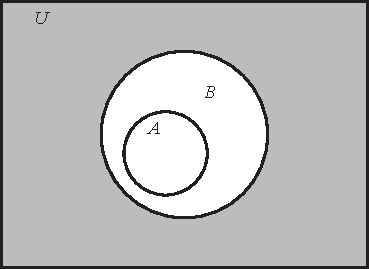
\includegraphics[width=\linewidth]{external/figps-asubsetb2.pdf}
\end{image}%
\tcblower
\end{figureptx}%
From the Venn diagram, it appears that \(A \cap B^c = \emptyset\). This means that \(A\) and \(B^c\) are disjoint. The preceding example suggests that the following proposition is true: \begin{quote}%
If \(A \subseteq B\), then \(A \cap B^c = \emptyset\).\end{quote}
 If we would like to prove this proposition, a reasonable ``backward question'' is, ``How do we prove that a set \(\left( \text{ namely } A \cap B^c \right)\) is equal to the empty set?''%
\par
This question seems difficult to answer since how do we prove that a set is empty? This is an instance where proving the contrapositive or using a proof by contradiction could be reasonable approaches. To illustrate these methods, let us assume the proposition we are trying to prove is of the following form: \begin{quote}%
If \(P\), then \(T = \emptyset\).\end{quote}
 If we choose to prove the contrapositive or use a proof by contradiction, we will assume that \(T \ne \emptyset\). These methods can be outlined as follows:%
\begin{itemize}[label=\textbullet]
\item{}The contrapositive of ``If \(P\), then \(T = \emptyset\)'' is, ``If \(T \ne \emptyset\), then \(\mynot P\).'' So in this case, we would assume \(T \ne \emptyset\) and try to prove \(\mynot P\).%
\item{}Using a proof by contradiction, we would assume \(P\) and assume that \(T \ne \emptyset\). From these two assumptions, we would attempt to derive a contradiction.%
\end{itemize}
One advantage of these methods is that when we assume that \(T \ne \emptyset\), then we know that there exists an element in the set \(T\). We can then use that element in the rest of the proof. We will prove one of the conditional statements for \hyperref[x:proposition:P_subsetprop]{Proposition~{\xreffont\ref{x:proposition:P_subsetprop}}, p.\,\pageref{x:proposition:P_subsetprop}} by proving its contrapositive. The proof of the other conditional statement associated with \hyperref[x:proposition:P_subsetprop]{Proposition~{\xreffont\ref{x:proposition:P_subsetprop}}, p.\,\pageref{x:proposition:P_subsetprop}} is \hyperlink{x:exercise:exer_subsetprop}{Exercise~{\xreffont 10}, p.\,\pageref{x:exercise:exer_subsetprop}}.%
\begin{proposition}{}{}{x:proposition:P_subsetprop}%
Let \(A\) and \(B\) be subsets of some universal set. Then \(A \subseteq B\) if and only if \(A \cap B^c = \emptyset\).%
\end{proposition}
\begin{proof}{}{g:proof:idm823196056}
Let \(A\) and \(B\) be subsets of some universal set. We will first prove that if \(A \subseteq B\), then \(A \cap B^c = \emptyset\), by proving its contrapositive. That is, we will prove \begin{quote}%
If \(A \cap B^c \ne \emptyset\), then \(A \not \subseteq B\).\end{quote}
 So assume that \(A \cap B^c \ne \emptyset\). We will prove that \(A \not \subseteq B\) by proving that there must exist an element \(x\) such that \(x \in A\) and \(x \notin B\).%
\par
Since \(A \cap B^c  \ne \emptyset\), there exists an element \(x\) that is in \(A \cap B^c\). This means that%
\begin{equation*}
x \in A\text{  and  } x \in B^c\text{.}
\end{equation*}
Now, the fact that \(x \in B^c\) means that \(x \notin B\). Hence, we can conclude that%
\begin{equation*}
x \in A\text{  and  } x \notin B\text{.}
\end{equation*}
This means that \(A \not \subseteq B\), and hence, we have proved that if \(A \cap B^c \ne \emptyset\), then \(A \not \subseteq B\), and therefore, we have proved that if \(A \subseteq B\), then \(A \cap B^c = \emptyset\).%
\par
The proof that if \(A \cap B^c = \emptyset\), then \(A \subseteq B\) is \hyperlink{x:exercise:exer_subsetprop}{Exercise~{\xreffont 10}, p.\,\pageref{x:exercise:exer_subsetprop}}.%
\end{proof}
\begin{inlineexercise}{Proving Two Sets Are Disjoint.}{x:exercise:prog_disjointsets}%
Proof: It has been noted that it is often possible to prove that two sets are disjoint by using a proof by contradiction. In this case, we assume that the two sets are not disjoint and hence, their intersection is not empty. Use this method to prove that the following two sets are disjoint.%
\begin{equation*}
A = \{ x \in \Z \mid x \equiv 3 \pmod 12 \}  \text{ and }   
B = \{ y \in \Z \mid y \equiv 2 \pmod 8 \}\text{.}
\end{equation*}
%
\space\hyperlink{g:solution:idm823186712-back}{[Solution]}\end{inlineexercise}%
\end{subsectionptx}
%
%
\typeout{************************************************}
\typeout{Subsection  A Final Comment}
\typeout{************************************************}
%
\begin{subsectionptx}{A Final Comment}{}{A Final Comment}{}{}{g:subsection:idm823182616}
\index{element-chasing proof}%
\index{proof!element-chasing}%
\index{choose-an-element method}%
We have used the choose-an-element method to prove \hyperref[x:proposition:P_SissubsetT]{Proposition~{\xreffont\ref{x:proposition:P_SissubsetT}}, p.\,\pageref{x:proposition:P_SissubsetT}}, \hyperref[x:proposition:P_setdifference]{Proposition~{\xreffont\ref{x:proposition:P_setdifference}}, p.\,\pageref{x:proposition:P_setdifference}}, and \hyperref[x:proposition:P_subsetprop]{Proposition~{\xreffont\ref{x:proposition:P_subsetprop}}, p.\,\pageref{x:proposition:P_subsetprop}}. Proofs involving sets that use this method are sometimes referred to as \terminology{element-chasing proofs.} This name is used since the basic method is to choose an arbitrary element from one set and ``chase it'' until you prove it must be in another set.%
\end{subsectionptx}
%
%
\typeout{************************************************}
\typeout{Exercises  Exercises}
\typeout{************************************************}
%
\begin{exercises-subsection}{Exercises}{}{Exercises}{}{}{g:exercises:idm823175704}
\begin{divisionexercise}{1}{}{}{x:exercise:exer_sec42-2}%
Let \(A = \left\{ {\left. {x \in \mathbb{R}} \right| x^2 \lt 4} \right\}\) and let \(B = \left\{ {x \in \mathbb{R}\left. \right| x \lt 2} \right\}\).%
\begin{enumerate}[font=\bfseries,label=(\alph*),ref=\alph*]
\item{}Is \(A \subseteq B\)? Justify your conclusion with a proof or a counterexample.%
\space\hyperlink{g:answer:idm823167384-back}{[Answer]}\item{}Is \(B \subseteq A\)? Justify your conclusion with a proof or a counterexample.%
\space\hyperlink{g:answer:idm823172120-back}{[Answer]}\end{enumerate}
\end{divisionexercise}%
\begin{divisionexercise}{2}{}{}{x:exercise:exer_sec42-3}%
Let \(A\), \(B\), and \(C\) be subsets of a universal set \(U\).%
\begin{enumerate}[font=\bfseries,label=(\alph*),ref=\alph*]
\item{}Draw a Venn diagram with \(A \subseteq B\) and \(B \subseteq C\). Does it appear that \(A \subseteq C\)?%
\item{}Prove the following proposition: \begin{quote}%
If \(A \subseteq B\) and \(B \subseteq C\), then \(A \subseteq C\).\end{quote}
%
\par
Note: This may seem like an obvious result. However, one of the reasons for this exercise is to provide practice at properly writing a proof that one set is a subset of another set. So we should start the proof by assuming that \(A \subseteq B\) and \(B \subseteq C\). Then we should choose an arbitrary element of \(A\).%
\end{enumerate}
\end{divisionexercise}%
\begin{divisionexercise}{3}{}{}{x:exercise:exer_modsubset}%
Let \(A = \{ x \in \mathbb{Z} \mid x \equiv 7 \pmod 8 \}\) and \(B = \{ x \in \mathbb{Z} \mid x \equiv 3 \pmod 4 \}\).%
\begin{enumerate}[font=\bfseries,label=(\alph*),ref=\alph*]
\item{}List at least five different elements of the set \(A\) and at least five elements of the set \(B\).%
\space\hyperlink{g:answer:idm823153304-back}{[Answer]}\item{}Is \(A \subseteq B\)? Justify your conclusion with a proof or a counterexample.%
\space\hyperlink{g:answer:idm823157016-back}{[Answer]}\item{}Is \(B \subseteq A\)? Justify your conclusion with a proof or a counterexample.%
\space\hyperlink{g:answer:idm823143960-back}{[Answer]}\end{enumerate}
\end{divisionexercise}%
\begin{divisionexercise}{4}{}{}{x:exercise:exer_modsubset2}%
Let \(C = \{ x \in \mathbb{Z} \mid x \equiv 7 \pmod {9} \}\) and \(D = \{ x \in \mathbb{Z} \mid x \equiv 1 \pmod {3} \}\).%
\begin{enumerate}[font=\bfseries,label=(\alph*),ref=\alph*]
\item{}List at least five different elements of the set \(C\) and at least five elements of the set \(D\).%
\item{}Is \(C \subseteq D\)? Justify your conclusion with a proof or a counterexample.%
\item{}Is \(D \subseteq C\)? Justify your conclusion with a proof or a counterexample.%
\end{enumerate}
\end{divisionexercise}%
\begin{divisionexercise}{5}{}{}{x:exercise:exer51_modsets}%
In each case, determine if \(A \subseteq B\), \(B \subseteq A\), \(A = B\), or \(A \cap B = \emptyset\) or none of these.%
\begin{enumerate}[font=\bfseries,label=(\alph*),ref=\alph*]
\item{}\(A = \left\{ x \in \Z \mid x \equiv 2 \pmod 3 \right\}\) and \(B = \left\{ y \in \Z \mid 6 \text{ divides } (2y - 4) \right\}\).%
\space\hyperlink{g:answer:idm823139352-back}{[Answer]}\item{}\(A = \left\{ x \in \Z \mid x \equiv 3 \pmod 4 \right\}\) and \(B = \left\{ y \in \Z \mid 3 \text{ divides } (y - 2) \right\}\).%
\item{}\(A = \left\{ x \in \Z \mid x \equiv 1 \pmod 5 \right\}\) and \(B = \left\{ y \in \Z \mid y \equiv 7 \pmod 10 \right\}\).%
\space\hyperlink{g:answer:idm823133208-back}{[Answer]}\end{enumerate}
\end{divisionexercise}%
\begin{divisionexercise}{6}{}{}{g:exercise:idm823124376}%
To prove the following set equalities, it may be necessary to use some of the properties of positive and negative real numbers. For example, it may be necessary to use the facts that:%
\begin{itemize}[label=\textbullet]
\item{}The product of two real numbers is positive if and only if the two real numbers are either both positive or both negative.%
\item{}The product of two real numbers is negative if and only if one of the two numbers is positive and the other is negative.%
\end{itemize}
For example, if \(x \left( x - 2 \right) \lt 0\), then we can conclude that either (1) \(x \lt 0\) and \(x - 2 > 0\) or (2) \(x > 0\) and \(x - 2 \lt 0\). However, in the first case, we must have \(x \lt 0\) and \(x > 2\), and this is impossible. Therefore, we conclude that \(x > 0\) and \(x - 2 \lt 0\), which means that \(0 \lt x \lt 2\).%
\par
Use the choose-an-element method to prove each of the following:%
\begin{enumerate}[font=\bfseries,label=(\alph*),ref=\alph*]
\item{}\(\left\{x \in \R \mid x^2 - 3x - 10 \lt 0 \right\} = \left\{ x \in \R \mid -2 \lt x 
\lt 5 \right\}\)%
\item{}\(\left\{x \in \R \mid x^2 - 5x + 6 \lt 0 \right\} = \left\{ x \in \R \mid 2 
\lt x \lt 3 \right\}\)%
\item{}\(\left\{ x \in \R \mid x^2 \geq 4 \right\} = \left\{ x \in \R \mid x 
\leq -2 \right\} \cup \left\{ x \in \R \mid x \geq 2 \right\}\)%
\end{enumerate}
\end{divisionexercise}%
\begin{divisionexercise}{7}{}{}{x:exercise:exer_intersectandunion}%
Let \(A\) and \(B\) be subsets of some universal set \(U\). Prove each of the following:%
\begin{enumerate}[font=\bfseries,label=(\alph*),ref=\alph*]
\item{}\(A \cap B \subseteq A\)%
\space\hyperlink{g:answer:idm823113496-back}{[Answer]}\item{}\(A \subseteq A \cup B\)%
\space\hyperlink{g:answer:idm823115672-back}{[Answer]}\item{}\(A \cap A = A\)%
\item{}\(A \cup A = A\)%
\item{}\(A \cap \emptyset = \emptyset\)%
\space\hyperlink{g:answer:idm823104408-back}{[Answer]}\item{}\(A \cup \emptyset = A\)%
\end{enumerate}
\end{divisionexercise}%
\begin{divisionexercise}{8}{}{}{x:exercise:exer_sec43-2}%
Let \(A\) and \(B\) be subsets of some universal set \(U\). From \hyperref[x:proposition:P_subsetandcomp]{Proposition~{\xreffont\ref{x:proposition:P_subsetandcomp}}, p.\,\pageref{x:proposition:P_subsetandcomp}}, we know that if \(A \subseteq B\), then \(B^c \subseteq A^c\). Now prove the following proposition: \begin{quote}%
For all sets \(A\) and \(B\) that are subsets of some universal set \(U\), \(A \subseteq B\) if and only if \(B^c \subseteq A^c\).\end{quote}
%
\end{divisionexercise}%
\begin{divisionexercise}{9}{}{}{x:exercise:exer_sec42-6}%
Is the following proposition true or false? Justify your conclusion with a proof or a counterexample. \begin{quote}%
For all sets \(A\) and \(B\) that are subsets of some universal set \(U\), the sets \(A \cap B\) and \(A - B\) are disjoint.\end{quote}
%
\end{divisionexercise}%
\begin{divisionexercise}{10}{}{}{x:exercise:exer_subsetprop}%
Complete the proof of \hyperref[x:proposition:P_subsetprop]{Proposition~{\xreffont\ref{x:proposition:P_subsetprop}}, p.\,\pageref{x:proposition:P_subsetprop}} by proving the following conditional statement: \begin{quote}%
Let \(A\) and \(B\) be subsets of some universal set. If \(A \cap B^c = \emptyset\), then \(A \subseteq B\) .\end{quote}
%
\space\hyperlink{g:hint:idm823091352-back}{[Hint]}\end{divisionexercise}%
\begin{divisionexercise}{11}{}{}{x:exercise:exer_sec42-disjoint}%
Let \(A\), \(B\), \(C\), and \(D\) be subsets of some universal set \(U\). Are the following propositions true or false? Justify your conclusions.%
\begin{enumerate}[font=\bfseries,label=(\alph*),ref=\alph*]
\item{}If \(A \subseteq B\) and \(C \subseteq D\) and \(A\) and \(C\) are disjoint, then \(B\) and \(D\) are disjoint.%
\item{}If \(A \subseteq B\) and \(C \subseteq D\) and \(B\) and \(D\) are disjoint, then \(A\) and \(C\) are disjoint.%
\end{enumerate}
\end{divisionexercise}%
\begin{divisionexercise}{12}{}{}{x:exercise:exer_unionandintersect}%
Let \(A\), \(B\), and \(C\) be subsets of a universal set \(U\). Prove:%
\begin{enumerate}[font=\bfseries,label=(\alph*),ref=\alph*]
\item{}If \(A \subseteq B\), then \(A \cap C \subseteq B \cap C\).%
\space\hyperlink{g:answer:idm823082776-back}{[Answer]}\item{}If \(A \subseteq B\), then \(A \cup C \subseteq B \cup C\).%
\end{enumerate}
\end{divisionexercise}%
\begin{divisionexercise}{13}{}{}{x:exercise:exer_sec42-unionandintersect}%
Let \(A\), \(B\), and \(C\) be subsets of a universal set \(U\). Are the following propositions true or false? Justify your conclusions.%
\begin{enumerate}[font=\bfseries,label=(\alph*),ref=\alph*]
\item{}If \(A \cap C \subseteq B \cap C\), then \(A \subseteq B\).%
\item{}If \(A \cup C \subseteq B \cup C\), then \(A \subseteq B\).%
\item{}If \(A \cup C = B \cup C\), then \(A = B\).%
\item{}If \(A \cap C = B \cap C\), then \(A = B\).%
\item{}If \(A \cup C = B \cup C\) and \(A \cap C = B \cap C\), then \(A = B\).%
\end{enumerate}
\end{divisionexercise}%
\begin{divisionexercise}{14}{}{}{g:exercise:idm823064728}%
Prove the following proposition: \begin{quote}%
For all sets \(A\), \(B\), and \(C\) that are subsets of some universal set, if \(A \cap B = A \cap C\) and \(A^c \cap B = A^c \cap C\), then \(B = C\).\end{quote}
%
\end{divisionexercise}%
\begin{divisionexercise}{15}{}{}{x:exercise:exer42_setstruefalse}%
Are the following biconditional statements true or false? Justify your conclusion. If a biconditional statement is found to be false, you should clearly determine if one of the conditional statements within it is true and provide a proof of this conditional statement.%
\begin{enumerate}[font=\bfseries,label=(\alph*),ref=\alph*]
\item{}For all subsets \(A\) and \(B\) of some universal set \(U\), \(A \subseteq B\) if and only if \(A \cap B^c = \emptyset\).%
\space\hyperlink{g:answer:idm823330328-back}{[Answer]}\item{}For all subsets \(A\) and \(B\) of some universal set \(U\), \(A \subseteq B\) if and only if \(A \cup B = B\).%
\space\hyperlink{g:answer:idm823051048-back}{[Answer]}\item{}For all subsets \(A\) and \(B\) of some universal set \(U\), \(A \subseteq B\) if and only if \(A \cap B = A\).%
\item{}For all subsets \(A\), \(B\), and \(C\) of some universal set \(U\), \(A \subseteq B \cup C\) if and only if \(A \subseteq B\) or \(A \subseteq C\).%
\item{}For all subsets \(A\), \(B\), and \(C\) of some universal set \(U\), \(A \subseteq B \cap C\) if and only if \(A \subseteq B\) and \(A \subseteq C\).%
\end{enumerate}
\end{divisionexercise}%
\begin{divisionexercise}{16}{}{}{g:exercise:idm823037736}%
Let \(S\), \(T\), \(X\), and \(Y\) be subsets of some universal set. Assume that%
\begin{multicols}{3}
\begin{enumerate}[label=\roman*]
\item{}\(S \cup T \subseteq X \cup Y\);%
\item{}\(S \cap T = \emptyset\); and%
\item{}\(X \subseteq S\).%
\end{enumerate}
\end{multicols}
%
\begin{enumerate}[font=\bfseries,label=(\alph*),ref=\alph*]
\item{}Using assumption (i), what conclusion(s) can be made if it is known that \(a \in T\)?%
\item{}Using assumption (ii), what conclusion(s) can be made if it is known that \(a \in T\)?%
\item{}Using all three assumptions, either prove that \(T \subseteq Y\) or explain why it is not possible to do so.%
\end{enumerate}
\end{divisionexercise}%
\begin{divisionexercise}{17}{Evaluation of Proofs.}{}{g:exercise:idm823027496}%
See the instructions for \hyperlink{x:exercise:exer_proofeval}{Exercise~{\xreffont 19}, p.\,\pageref{x:exercise:exer_proofeval}} from \hyperref[x:section:S_directproof]{Section~{\xreffont\ref{x:section:S_directproof}}, p.\,\pageref{x:section:S_directproof}}.%
\begin{enumerate}[font=\bfseries,label=(\alph*),ref=\alph*]
\item{}%
\begin{descriptionlist}
\begin{dlinarrow}{Proposition}{g:li:idm823025704}%
Let \(A\), \(B\), and \(C\) be subsets of some universal set. If \(A \not \subseteq B\) and \(B \not \subseteq C\), then \(A \not \subseteq C\).%
\end{dlinarrow}%
\begin{dlinarrow}{Proof}{g:li:idm823020840}%
We assume that \(A\), \(B\), and \(C\) are subsets of some universal set and that \(A \not \subseteq B\) and \(B \not \subseteq C\). This means that there exists an element \(x\) in \(A\) that is not in \(B\) and there exists an element \(x\) that is in \(B\) and not in \(C\). Therefore, \(x \in A\) and \(x \notin C\), and we have proved that \(A \not \subseteq C\).%
\end{dlinarrow}%
\end{descriptionlist}
%
\item{}%
\begin{descriptionlist}
\begin{dlinarrow}{Proposition}{g:li:idm823013672}%
Let \(A\), \(B\), and \(C\) be subsets of some universal set. If \(A \cap B = A \cap C\), then \(B = C\).%
\end{dlinarrow}%
\begin{dlinarrow}{Proof}{g:li:idm823013032}%
We assume that \(A \cap B = A \cap C\) and will prove that \(B = C\). We will first prove that \(B \subseteq C\).%
\par
So let \(x \in B\). If \(x \in A\), then \(x \in A \cap B\), and hence, \(x \in A \cap C\). From this we can conclude that \(x \in C\). If \(x \notin A\), then \(x \notin A \cap B\), and hence, \(x \notin A \cap C\). However, since \(x \notin A\), we may conclude that \(x \in C\). Therefore, \(B \subseteq C\).%
\par
The proof that \(C \subseteq B\) may be done in a similar manner. Hence, \(B = C\).%
\end{dlinarrow}%
\end{descriptionlist}
%
\item{}%
\begin{descriptionlist}
\begin{dlinarrow}{Proposition}{g:li:idm823003048}%
Let \(A\), \(B\), and \(C\) be subsets of some universal set. If \(A \not \subseteq B\) and \(B \subseteq C\), then \(A \not \subseteq C\).%
\end{dlinarrow}%
\begin{dlinarrow}{Proof}{g:li:idm823000104}%
Assume that \(A \not \subseteq B\) and \(B \subseteq C\). Since \(A \not \subseteq B\), there exists an element \(x\) such that \(x \in A\) and \(x \notin B\). Since \(B \subseteq C\), we may conclude that \(x \notin C\). Hence, \(x \in A\) and \(x \notin C\), and we have proved that \(A \not \subseteq C\).%
\end{dlinarrow}%
\end{descriptionlist}
%
\end{enumerate}
\end{divisionexercise}%
\begin{activity}{Using the Choose-an-Element Method in a Different Setting.}{x:activity:exer52-choose}%
We have used the choose-an-element method to prove results about sets. This method, however, is a general proof technique and can be used in settings other than set theory. It is often used whenever we encounter a universal quantifier in a statement in the backward process. Consider the following proposition. \begin{proposition}{}{}{x:proposition:P_divlinearcomb}%
Let a, b, and t be integers with \(t \ne 0\). If t divides a and t divides b, then for all integers x and y, t divides (ax + by).%
\end{proposition}
%
\begin{enumerate}[font=\bfseries,label=(\alph*),ref=\alph*]
\item\label{x:task:A_divlincomb1}Whenever we encounter a new proposition, it is a good idea to explore the proposition by looking at specific examples. For example, let \(a = 20\), \(b = 12\), and \(t = 4\). In this case, \(t \mid a\) and \(t \mid b\). In each of the following cases, determine the value of \(\left(ax + by \right)\) and determine if \(t\) divides \(\left(ax + by\right)\).%
\begin{enumerate}[font=\bfseries,label=(\roman*),ref=\theenumi.\roman*]
\item{}\(x=1, y=1\)%
\item{}\(x=1, y=-1\)%
\item{}\(x=2, y=2\)%
\item{}\(x=2, y=-3\)%
\item{}\(x=-2, y=3\)%
\item{}\(x=-2, y=-5\)%
\end{enumerate}
\item{}Repeat \hyperref[x:task:A_divlincomb1]{Task~{\xreffont\ref{x:activity:exer52-choose}}.{\xreffont\ref{x:task:A_divlincomb1}}, p.\,\pageref{x:task:A_divlincomb1}} with \(a = 21\), \(b = - 6\), and \(t = 3\).%
\par
Notice that the conclusion of the conditional statement in this proposition involves the universal quantifier. So in the backward process, we would have \begin{quote}%
\(Q\): For all integers \(x\) and \(y\), \(t\) divides \(ax + by\).\end{quote}
 The ``elements'' in this sentence are the integers \(x\) and \(y\). In this case, these integers have no ``given property'' other than that they are integers. The ``something that happens'' is that \(t\) divides \(\left(ax + by\right)\). This means that in the forward process, we can use the hypothesis of the proposition and choose integers \(x\) and \(y\). That is, in the forward process, we could have \begin{quote}%
\(P\): \(a\), \(b\), and \(t\) are integers with \(t \ne 0\), \(t\) divides \(a\) and \(t\) divides \(b\). \textbackslash{}item \(P1\): Let \(x \in \Z\) and let \(y \in \Z\).\end{quote}
%
\item{}Complete the following proof of \hyperref[x:proposition:P_divlinearcomb]{Proposition~{\xreffont\ref{x:proposition:P_divlinearcomb}}, p.\,\pageref{x:proposition:P_divlinearcomb}}. \begin{proof}{}{g:proof:idm822971048}
Let \(a\), \(b\), and \(t\) be integers with \(t \ne 0\), and assume that \(t\) divides \(a\) and \(t\) divides \(b\). We will prove that for all integers \(x\) and \(y\), \(t\) divides \(\left(ax + by\right)\).%
\par
So let \(x \in \Z\) and let \(y \in \Z\). Since \(t\) divides \(a\), there exists an integer \(m\) such that \(\ldots \).%
\end{proof}
%
\end{enumerate}
\end{activity}%
\end{exercises-subsection}
\end{sectionptx}
%
%
\typeout{************************************************}
\typeout{Section 5.3 Properties of Set Operations}
\typeout{************************************************}
%
\begin{sectionptx}{Properties of Set Operations}{}{Properties of Set Operations}{}{}{x:section:S_setproperties}
%
%
\typeout{************************************************}
\typeout{Beginning Activity  Beginning Activity 1: Exploring a Relationship between Two Sets}
\typeout{************************************************}
%
\begin{worksheet-subsection}{Beginning Activity 1: Exploring a Relationship between Two Sets}{}{Beginning Activity 1: Exploring a Relationship between Two Sets}{}{}{x:worksheet:PA_workingwithvenn2}
Let \(A\) and \(B\) be subsets of some universal set \(U\).%
\begin{divisionexercise}{1}{}{}{x:exercise:PA_workingwithvenn2-1}%
Draw two general Venn diagrams for the sets \(A\) and \(B\). On one, shade the region that represents \(\left( {A \cup B} \right)^c\), and on the other, shade the region that represents \(A^c \cap B^c\). Explain carefully how you determined these regions.%
\end{divisionexercise}%
\begin{divisionexercise}{2}{}{}{g:exercise:idm822961064}%
Based on the Venn diagrams in \hyperlink{x:exercise:PA_workingwithvenn2-1}{Exercise~{\xreffont 1}, p.\,\pageref{x:exercise:PA_workingwithvenn2-1}}, what appears to be the relationship between the sets \(\left( {A \cup B} \right)^c\) and \(A^c \cap B^c\)?%
\end{divisionexercise}%
Some of the properties of set operations are closely related to some of the logical operators we studied in \hyperref[x:section:S_2logop]{Section~{\xreffont\ref{x:section:S_2logop}}, p.\,\pageref{x:section:S_2logop}}. This is due to the fact that set intersection is defined using a conjunction (and), and set union is defined using a disjunction (or). For example, if \(A\) and \(B\) are subsets of some universal set \(U\), then an element \(x\) is in \(A \cup B\) if and only if \(x \in A\) or \(x \in B\).%
\begin{divisionexercise}{3}{}{}{x:exercise:part1PA1}%
Use one of De Morgan's Laws (\hyperref[x:theorem:T_logequiv]{Theorem~{\xreffont\ref{x:theorem:T_logequiv}}, p.\,\pageref{x:theorem:T_logequiv}} to explain carefully what it means to say that an element \(x\) is not in \(A \cup B\).%
\end{divisionexercise}%
\begin{divisionexercise}{4}{}{}{g:exercise:idm822951336}%
What does it mean to say that an element \(x\) is in \(A^c\)? What does it mean to say that an element \(x\) is in \(B^c\)?%
\end{divisionexercise}%
\begin{divisionexercise}{5}{}{}{x:exercise:part3PA1}%
Explain carefully what it means to say that an element \(x\) is in \(A^c \cap B^c\).%
\end{divisionexercise}%
\begin{divisionexercise}{6}{}{}{g:exercise:idm822953384}%
Compare your response in \hyperlink{x:exercise:part1PA1}{Exercise~{\xreffont 3}, p.\,\pageref{x:exercise:part1PA1}} to your response in \hyperlink{x:exercise:part3PA1}{Exercise~{\xreffont 5}, p.\,\pageref{x:exercise:part3PA1}}. Are they equivalent? Explain.%
\end{divisionexercise}%
\begin{divisionexercise}{7}{}{}{g:exercise:idm822947752}%
How do you think the sets \(\left( {A \cup B} \right)^c\) and \(A^c \cap B^c\) are related? Is this consistent with the Venn diagrams from \hyperlink{x:exercise:PA_workingwithvenn2-1}{Exercise~{\xreffont 1}, p.\,\pageref{x:exercise:PA_workingwithvenn2-1}}?%
\end{divisionexercise}%
\end{worksheet-subsection}
%
%
\typeout{************************************************}
\typeout{Beginning Activity  Beginning Activity 2: Proving that Statements Are Equivalent}
\typeout{************************************************}
%
\begin{worksheet-subsection}{Beginning Activity 2: Proving that Statements Are Equivalent}{}{Beginning Activity 2: Proving that Statements Are Equivalent}{}{}{x:worksheet:PA_provingequiv}
\begin{divisionexercise}{1}{}{}{g:exercise:idm822938024}%
Let \(X\), \(Y\), and \(Z\) be statements. Complete a truth table for \(\left[ {\left( {X \to Y} \right) \wedge \left( {Y \to Z} \right)} \right] \to 
\left( {X \to Z} \right)\).%
\end{divisionexercise}%
\begin{divisionexercise}{2}{}{}{g:exercise:idm822941992}%
Assume that \(P\), \(Q\), and \(R\) are statements and that we have proven that the following conditional statements are true:%
\begin{multicols}{2}
\begin{itemize}[label=\textbullet]
\item{}If \(P\) then \(Q\) \(\left( {P \to Q} \right)\).%
\item{}If \(Q\) then \(R\) \(\left( {Q \to R} \right)\).%
\item{}If \(R\) then \(P\) \(\left( {R \to P} \right)\).%
\end{itemize}
\end{multicols}
Explain why each of the following statements is true.%
\begin{enumerate}[font=\bfseries,label=(\alph*),ref=\alph*]
\item{}\(P\) if and only if \(Q\) \(\left( {P \leftrightarrow Q} \right)\).%
\item{}\(Q\) if and only if \(R\) \(\left( {Q \leftrightarrow R} \right)\).%
\item{}\(R\) if and only if \(P\) \(\left( {R \leftrightarrow P} \right)\).%
\end{enumerate}
Remember that \(X \leftrightarrow Y\) is logically equivalent to \(\left( {X \to Y} \right) \wedge \left( {Y \to X} \right)\).%
\end{divisionexercise}%
\end{worksheet-subsection}
%
%
\typeout{************************************************}
\typeout{Subsection  Algebra of Sets \textemdash{} Part 1}
\typeout{************************************************}
%
\begin{subsectionptx}{Algebra of Sets \textemdash{} Part 1}{}{Algebra of Sets \textemdash{} Part 1}{}{}{g:subsection:idm822925224}
\index{algebra of sets}%
\index{set theory}%
This section contains many results concerning the properties of the set operations. We have already proved some of the results. Others will be proved in this section or in the exercises. The primary purpose of this section is to have in one place many of the properties of set operations that we may use in later proofs. These results are part of what is known as the \terminology{algebra of sets} or as \terminology{set theory}.%
\begin{theorem}{}{}{x:theorem:T_intersectandunion}%
Let \(A\), \(B\), and \(C\) be subsets of some universal set \(U\). Then%
\begin{itemize}[label=\textbullet]
\item{}\(A \cap B \subseteq A\text{ and } A \subseteq A \cup B\).%
\item{}If \(A \subseteq B\), then \(A \cap C \subseteq B \cap C\) and \(A \cup C \subseteq B \cup C\).%
\end{itemize}
%
\end{theorem}
\begin{proof}{}{g:proof:idm822918824}
The first part of this theorem was included in \hyperlink{x:exercise:exer_intersectandunion}{Exercise~{\xreffont 7}, p.\,\pageref{x:exercise:exer_intersectandunion}} from \hyperref[x:section:S_provingset]{Section~{\xreffont\ref{x:section:S_provingset}}, p.\,\pageref{x:section:S_provingset}}. The second part of the theorem was \hyperlink{x:exercise:exer_unionandintersect}{Exercise~{\xreffont 12}, p.\,\pageref{x:exercise:exer_unionandintersect}} from \hyperref[x:section:S_provingset]{Section~{\xreffont\ref{x:section:S_provingset}}, p.\,\pageref{x:section:S_provingset}}.%
\end{proof}
The next theorem provides many of the properties of set operations dealing with intersection and union. Many of these results may be intuitively obvious, but to be complete in the development of set theory, we should prove all of them. We choose to prove only some of them and leave some as exercises.%
\begin{theorem}{Algebra of Set Operations.}{}{x:theorem:T_algebraofsets}%
Let \(A\), \(B\), and \(C\) be subsets of some universal set \(U\). Then all of the following equalities hold.%
\begin{descriptionlist}
\begin{dlimedium}{Properties of the Empty Set and the Universal Set}{g:li:idm822920616}%
\index{empty set!properties}\index{universal set!properties}%
\begin{align*}
A \cap \emptyset \amp = \emptyset \amp A \cap U \amp = A\\
A \cup \emptyset \amp = A \amp A \cup U \amp = U
\end{align*}
%
\end{dlimedium}%
\begin{dlimedium}{Idempotent Laws}{g:li:idm822912424}%
\index{idempotent laws for sets}%
\begin{align*}
A \cap A \amp = A \amp A \cup A \amp = A
\end{align*}
%
\end{dlimedium}%
\begin{dlimedium}{Commutative Laws}{g:li:idm822908968}%
\index{commutative laws!for sets}%
\begin{align*}
A \cap B \amp = B \cap A \amp A \cup B \amp = B \cup A
\end{align*}
%
\end{dlimedium}%
\begin{dlimedium}{Associative Laws}{g:li:idm822911912}%
\index{associative laws!for sets}%
\begin{align*}
\left( A \cap B \right) \cap C \amp = A \cap \left(B \cap C \right)\\
\left( A \cup B \right) \cup C \amp = A \cup \left(B \cup C \right)
\end{align*}
%
\end{dlimedium}%
\begin{dlimedium}{Distributive Laws}{g:li:idm822904744}%
\index{distributive laws!for sets}%
\begin{align*}
A \cap \left( B \cup C \right) \amp = \left( A \cap B \right) \cup 
\left( A \cap C \right)\\
A \cup \left( B \cap C \right) \amp = \left( A \cup B \right) \cap 
\left( A \cup C \right)
\end{align*}
%
\end{dlimedium}%
\end{descriptionlist}
%
\end{theorem}
Before proving some of these properties, we note that in \hyperref[x:section:S_provingset]{Section~{\xreffont\ref{x:section:S_provingset}}, p.\,\pageref{x:section:S_provingset}}, we learned that we can prove that two sets are equal by proving that each one is a subset of the other one. However, we also know that if \(S\) and \(T\) are both subsets of a universal set \(U\), then \begin{quote}%
\(S = T\) if and only if for each \(x \in U\), \({x \in S\text{ if and only if } x \in T}\).\end{quote}
%
\par
We can use this to prove that two sets are equal by choosing an element from one set and chasing the element to the other set through a sequence of ``if and only if'' statements. We now use this idea to prove one of the commutative laws.%
\end{subsectionptx}
%
%
\typeout{************************************************}
\typeout{Subsection  Proof of One of the Commutative Laws in Theorem~{\xreffont\ref*{x:theorem:T_algebraofsets}}}
\typeout{************************************************}
%
\begin{subsectionptx}{Proof of One of the Commutative Laws in Theorem~{\xreffont\ref*{x:theorem:T_algebraofsets}}}{}{Proof of One of the Commutative Laws in Theorem~{\xreffont\ref*{x:theorem:T_algebraofsets}}}{}{}{g:subsection:idm822898856}
\begin{proof}{}{g:proof:idm822903976}
We will prove that \(A \cap B = B \cap A\). Let \(x \in U\). Then%
\begin{equation}
x \in A \cap B\text{  if and only if  } x \in A\text{  and  } x \in B\text{.}\label{x:men:eq_4a}
\end{equation}
However, we know that if \(P\) and \(Q\) are statements, then \(P \wedge Q\) is logically equivalent to \(Q \wedge P\). Consequently, we can conclude that%
\begin{equation}
x \in A\text{ and } x \in B\text{  if and only if } \;x \in B\text{ and } x \in A\text{.}\label{x:men:eq_4b}
\end{equation}
Now we know that%
\begin{equation}
x \in B\text{ and } x \in A\text{  if and only if  } x \in B \cap A\text{.}\label{x:men:eq_4c}
\end{equation}
This means that we can use \hyperref[x:men:eq_4a]{({\xreffont\ref{x:men:eq_4a}})}, \hyperref[x:men:eq_4b]{({\xreffont\ref{x:men:eq_4b}})}, and \hyperref[x:men:eq_4c]{({\xreffont\ref{x:men:eq_4c}})} to conclude that%
\begin{equation*}
x \in A \cap B\text{  if and only if  } x \in B \cap A\text{,}
\end{equation*}
and, hence, we have proved that \(A \cap B = B \cap A\).%
\end{proof}
\begin{inlineexercise}{Exploring a Distributive Property.}{x:exercise:prog_workingvenn3}%
We can use Venn diagrams to explore the more complicated properties in \hyperref[x:theorem:T_algebraofsets]{Theorem~{\xreffont\ref{x:theorem:T_algebraofsets}}, p.\,\pageref{x:theorem:T_algebraofsets}}, such as the associative and distributive laws. To that end, let \(A\), \(B\), and \(C\) be subsets of some universal set \(U\).%
\begin{enumerate}[font=\bfseries,label=(\alph*),ref=\alph*]
\item\label{x:task:A_workingvenn3-1}Draw two general Venn diagrams for the sets \(A\), \(B\), and \(C\). On one, shade the region that represents \(A \cup \left( {B \cap C} \right)\), and on the other, shade the region that represents \(\left( {A \cup B} \right) \cap \left( {A \cup C} \right)\). Explain carefully how you determined these regions.%
\space\hyperlink{g:solution:idm822881704-back}{[Solution]}\item{}Based on the Venn diagrams in \hyperref[x:task:A_workingvenn3-1]{Task~{\xreffont\ref{x:exercise:prog_workingvenn3}}.{\xreffont\ref{x:task:A_workingvenn3-1}}, p.\,\pageref{x:task:A_workingvenn3-1}}, what appears to be the relationship between the sets \(A \cup \left( {B \cap C} \right)\) and \(\left( {A \cup B} \right) \cap \left( {A \cup C} \right)\)?%
\space\hyperlink{g:solution:idm822881192-back}{[Solution]}\end{enumerate}
\end{inlineexercise}%
\end{subsectionptx}
%
%
\typeout{************************************************}
\typeout{Subsection  Proof of One of the Distributive Laws in Theorem~{\xreffont\ref*{x:theorem:T_algebraofsets}}}
\typeout{************************************************}
%
\begin{subsectionptx}{Proof of One of the Distributive Laws in Theorem~{\xreffont\ref*{x:theorem:T_algebraofsets}}}{}{Proof of One of the Distributive Laws in Theorem~{\xreffont\ref*{x:theorem:T_algebraofsets}}}{}{}{g:subsection:idm822886312}
We will now prove the distributive law explored in \hyperref[x:exercise:prog_workingvenn3]{Progress Check~{\xreffont\ref{x:exercise:prog_workingvenn3}}, p.\,\pageref{x:exercise:prog_workingvenn3}}. Notice that we will prove two subset relations, and that for each subset relation, we will begin by choosing an arbitrary element from a set. Also notice how nicely a proof dealing with the union of two sets can be broken into cases.%
\begin{proof}{}{g:proof:idm822874408}
Let \(A\), \(B\), and \(C\) be subsets of some universal set \(U\). We will prove that \(A \cup \left( {B \cap C} \right) = \left( {A \cup B} \right) 
\cap \left( {A \cup C} \right)\) by proving that each set is a subset of the other set.%
\par
We will first prove that \(A \cup \left( {B \cap C} \right) \subseteq \left( {A \cup B} 
\right) \cap \left( {A \cup C} \right)\). We let \(x \in A \cup \left( {B \cap C} \right)\). Then \(x \in A\text{ or } x \in B \cap C\).%
\par
So in one case, if \(x \in A\), then \(x \in A \cup B\) and \(x \in A \cup C\). This means that \(x \in \left( {A \cup B} \right) \cap \left( {A \cup C} \right)\).%
\par
On the other hand, if \(x \in B \cap C\), then \(x \in B\) and \(x \in C\). But \(x \in B\) implies that \(x \in A \cup B\), and \(x \in C\) implies that \(x \in A \cup C\). Since \(x\) is in both sets, we conclude that \(x \in \left( {A \cup B} \right) \cap \left( {A \cup C} \right)\). So in both cases, we see that \(x \in \left( {A \cup B} \right) \cap \left( {A \cup C} \right)\), and this proves that \(A \cup \left( {B \cap C} \right) \subseteq \left( {A \cup B} \right) 
\cap \left( {A \cup C} \right)\).%
\par
We next prove that \(\left( {A \cup B} \right) \cap \left( {A \cup C} \right) 
\subseteq A \cup \left( {B \cap C} \right)\). So let \(y \in \left( {A \cup B} \right) \cap \left( {A \cup C} \right)\). Then, \(y \in A \cup B\text{ and } y \in A \cup C\). We must prove that \(y \in A \cup \left( {B \cap C} \right)\). We will consider the two cases where \(y \in A\) or \(y \notin A\). In the case where \(y \in A\), we see that \(y \in A \cup \left( {B \cap C} \right)\).%
\par
So we consider the case that \(y \notin A\). It has been established that \(y \in A \cup B\) and \(y \in A \cup C\). Since \(y \notin A\) and \(y \in A \cup B\), \(y\) must be an element of \(B\). Similarly, since \(y \notin A\) and \(y \in A \cup C\), \(y\) must be an element of \(C\). Thus, \(y \in B \cap C\) and, hence, \(y \in A \cup \left( {B \cap C} \right)\).%
\par
In both cases, we have proved that \(y \in A \cup \left( {B \cap C} \right)\). This proves that \(\left( {A \cup B} \right) \cap \left( {A \cup C} \right) 
\subseteq A \cup \left( {B \cap C} \right)\). The two subset relations establish the equality of the two sets. Thus, \(A \cup \left( {B \cap C} \right) = \left( {A \cup B} \right) 
\cap \left( {A \cup C} \right)\).%
\end{proof}
\end{subsectionptx}
%
%
\typeout{************************************************}
\typeout{Subsection  Important Properties of Set Complements}
\typeout{************************************************}
%
\begin{subsectionptx}{Important Properties of Set Complements}{}{Important Properties of Set Complements}{}{}{g:subsection:idm822860200}
The three main set operations are union, intersection, and complementation. \hyperref[x:theorem:T_algebraofsets]{Theorems~{\xreffont\ref{x:theorem:T_algebraofsets}}, p.\,\pageref{x:theorem:T_algebraofsets}} and \hyperref[x:theorem:T_intersectandunion]{Theorem~{\xreffont\ref{x:theorem:T_intersectandunion}}, p.\,\pageref{x:theorem:T_intersectandunion}} deal with properties of unions and intersections. The next theorem states some basic properties of complements and the important relations dealing with complements of unions and complements of intersections. Two relationships in the next theorem are known as \terminology{De Morgan's Laws} for sets and are closely related to De Morgan's Laws for statements.%
\begin{theorem}{}{}{x:theorem:T_propsofcomplements}%
Let \(A\) and \(B\) be subsets of some universal set \(U\). Then the following are true:%
\begin{descriptionlist}
\begin{dlimedium}{Basic Properties}{g:li:idm822848808}%
\(\left( A^c \right)^c = A\)%
\par
\(A - B = A \cap B^c\)%
\end{dlimedium}%
\begin{dlimedium}{Empty Set and Universal Set}{g:li:idm822855336}%
\(A - \emptyset = A\) and \(A - U = \emptyset\)%
\par
\({\emptyset}^c = U\) and \(U^c = \emptyset\)%
\end{dlimedium}%
\begin{dlimedium}{De Morgan's Laws}{g:li:idm822851368}%
\index{De Morgan's Laws!for sets}\(\left ({A \cap B} \right)^c = A^c \cup B^c\)%
\par
\(\left ({A \cup B} \right)^c = A^c \cap B^c\)%
\end{dlimedium}%
\begin{dlimedium}{Subsets and Complements}{g:li:idm822842280}%
\(\displaystyle A \subseteq B \text{ if and only if } B^c \subseteq A^c\)%
\end{dlimedium}%
\end{descriptionlist}
%
\end{theorem}
\begin{proof}{}{g:proof:idm822840232}
We will only prove one of De Morgan's Laws, namely, the one that was explored in \hyperref[x:worksheet:PA_workingwithvenn2]{Beginning Activty 1, p.\,\pageref{x:worksheet:PA_workingwithvenn2}}. The proofs of the other parts are left as exercises. Let \(A\) and \(B\) be subsets of some universal set \(U\). We will prove that \(\left( {A \cup B} \right)^c  = A^c  \cap B^c\) by proving that an element is in \(\left( {A \cup B} \right)^c\) if and only if it is in \(A^c  \cap B^c\). So let \(x\) be in the universal set \(U\). Then%
\begin{equation}
x \in \left( {A \cup B} \right)^c \text{  if and only if  }  x \notin A \cup B\text{,}\label{x:men:eq_4d}
\end{equation}
and%
\begin{equation}
x \notin A \cup B\text{  if and only if  } x \notin A\text{  and  } x \notin B\text{.}\label{x:men:eq_4e}
\end{equation}
Combining \hyperref[x:men:eq_4d]{({\xreffont\ref{x:men:eq_4d}})} and \hyperref[x:men:eq_4e]{({\xreffont\ref{x:men:eq_4e}})}, we see that%
\begin{equation}
x \in \left( {A \cup B} \right)^c \text{  if and only if  } x \notin A\text{  and  } x 
\notin B\text{.}\label{x:men:eq_4f}
\end{equation}
In addition, we know that%
\begin{equation}
x \notin A \text{  and  }  x \notin B \text{  if and only if  }  x \in A^c \text{  and  }  
x \in B^c\text{,}\label{x:men:eq_4g}
\end{equation}
and this is true if and only if \(x \in A^c  \cap B^c\). So we can use equation \hyperref[x:men:eq_4f]{({\xreffont\ref{x:men:eq_4f}})} and equation \hyperref[x:men:eq_4g]{({\xreffont\ref{x:men:eq_4g}})} to conclude that%
\begin{equation*}
x \in \left( {A \cup B} \right)^c \text{  if and only if  } x \in A^c  \cap B^c\text{,}
\end{equation*}
and, hence, that \(\left( {A \cup B} \right)^c  = A^c  \cap B^c\).%
\end{proof}
\begin{inlineexercise}{}{x:exercise:A_usingalgebrasets1}%
Draw two general Venn diagrams for the sets \(A\), \(B\), and \(C\). On one, shade the region that represents \(\left( {A \cup B} \right) - C\), and on the other, shade the region that represents \(\left( {A - C} \right) \cup \left( {B - C} \right)\). Explain carefully how you determined these regions and why they indicate that \(\left( {A \cup B} \right) - C = \left( {A - C} \right) \cup \left( {B - C} \right)\).%
\space\hyperlink{g:solution:idm822831016-back}{[Solution]}\end{inlineexercise}%
\begin{inlineexercise}{}{x:exercise:A_usingalgebrasets2}%
It is possible to prove the relationship suggested in \hyperref[x:exercise:A_usingalgebrasets1]{Progress Check~{\xreffont\ref{x:exercise:A_usingalgebrasets1}}, p.\,\pageref{x:exercise:A_usingalgebrasets1}} by proving that each set is a subset of the other set. However, the results in \hyperref[x:theorem:T_algebraofsets]{Theorems~{\xreffont\ref{x:theorem:T_algebraofsets}}, p.\,\pageref{x:theorem:T_algebraofsets}} and \hyperref[x:theorem:T_propsofcomplements]{Theorem~{\xreffont\ref{x:theorem:T_propsofcomplements}}, p.\,\pageref{x:theorem:T_propsofcomplements}} can be used to prove other results about set operations. When we do this, we say that we are using the algebra of sets to prove the result. For example, we can start by using one of the basic properties in \hyperref[x:theorem:T_propsofcomplements]{Theorem~{\xreffont\ref{x:theorem:T_propsofcomplements}}, p.\,\pageref{x:theorem:T_propsofcomplements}} to write%
\begin{equation*}
\left( {A \cup B} \right) - C = \left( {A \cup B} \right) \cap C^c\text{.}
\end{equation*}
%
\par
We can then use one of the commutative properties to write%
\begin{align*}
\left( {A \cup B} \right) - C \amp = \left( {A \cup B} \right) \cap C^c\\
\amp = C^c  \cap \left( {A \cup B} \right)\text{.}
\end{align*}
%
\par
Determine which properties from \hyperref[x:theorem:T_algebraofsets]{Theorem~{\xreffont\ref{x:theorem:T_algebraofsets}}, p.\,\pageref{x:theorem:T_algebraofsets}} and \hyperref[x:theorem:T_propsofcomplements]{Theorem~{\xreffont\ref{x:theorem:T_propsofcomplements}}, p.\,\pageref{x:theorem:T_propsofcomplements}} justify each of the last three steps in the following outline of the proof that \(\left( {A \cup B} \right) - C = \left( {A - C} \right) \cup \left( {B - C} 
\right)\).%
\begin{align*}
\left( {A \cup B} \right) - C \amp = \left( {A \cup B} \right) \cap C^c \amp  
\hyperref[x:theorem:T_propsofcomplements]{\text{Theorem {\xreffont\ref{x:theorem:T_propsofcomplements}}, p.\,\pageref{x:theorem:T_propsofcomplements}}}\\
\amp = C^c  \cap \left( {A \cup B} \right) \amp \text{ (Commutative Property) }\\
\amp = \left( C^c \cap A \right) \cup \left( C^c \cap B \right)\\
\amp = \left( A \cap C^c \right) \cup \left( B \cap C^c \right)\\
\amp = \left( A - C \right) \cup \left( B - C \right)
\end{align*}
%
\par
Note: It is sometimes difficult to use the properties in the theorems when the theorems use the same letters to represent the sets as those being used in the current problem. For example, one of the distributive properties from \hyperref[x:theorem:T_algebraofsets]{Theorem~{\xreffont\ref{x:theorem:T_algebraofsets}}, p.\,\pageref{x:theorem:T_algebraofsets}} can be written as follows: For all sets \(X\), \(Y\), and \(Z\) that are subsets of a universal set \(U\),%
\begin{equation*}
X \cap \left( Y \cup Z \right) = \left( X \cap Y \right) \cup \left( X \cap Z \right)\text{.}
\end{equation*}
%
\space\hyperlink{g:solution:idm822824360-back}{[Solution]}\end{inlineexercise}%
\end{subsectionptx}
%
%
\typeout{************************************************}
\typeout{Subsection  Proving that Statements Are Equivalent}
\typeout{************************************************}
%
\begin{subsectionptx}{Proving that Statements Are Equivalent}{}{Proving that Statements Are Equivalent}{}{}{g:subsection:idm822822184}
When we have a list of three statements \(P\), \(Q\), and \(R\) such that each statement in the list is equivalent to the other two statements in the list, we say that the three statements are equivalent. This means that each of the statements in the list implies each of the other statements in the list.%
\par
The purpose of \hyperref[x:worksheet:PA_provingequiv]{Beginning Activity 2, p.\,\pageref{x:worksheet:PA_provingequiv}} was to provide one way to prove that three (or more) statements are equivalent. The basic idea is to prove a sequence of conditional statements so that there is an unbroken chain of conditional statements from each statement to every other statement. This method of proof will be used in \hyperref[x:theorem:T_subsetequivs]{Theorem~{\xreffont\ref{x:theorem:T_subsetequivs}}, p.\,\pageref{x:theorem:T_subsetequivs}}.%
\begin{theorem}{}{}{x:theorem:T_subsetequivs}%
Let \(A\) and \(B\) be subsets of some universal set \(U\). The following are equivalent:%
\begin{multicols}{3}
\begin{enumerate}
\item\label{x:li:T_subsetitem1}{}\hypertarget{x:li:T_subsetitem1}{}\(\displaystyle A \subseteq B\)%
\item\label{x:li:T_subsetitem2}{}\hypertarget{x:li:T_subsetitem2}{}\(\displaystyle A \cap B^c = \emptyset\)%
\item\label{x:li:T_subsetitem3}{}\hypertarget{x:li:T_subsetitem3}{}\(\displaystyle A^c \cup B = U\)%
\end{enumerate}
\end{multicols}
%
\end{theorem}
\begin{proof}{}{g:proof:idm822812200}
To prove that these are equivalent conditions, we will prove that \hyperlink{x:li:T_subsetitem1}{Item~{\xreffont 1}, p.\,\pageref{x:li:T_subsetitem1}} implies \hyperlink{x:li:T_subsetitem2}{Item~{\xreffont 2}, p.\,\pageref{x:li:T_subsetitem2}}, that \hyperlink{x:li:T_subsetitem2}{Item~{\xreffont 2}, p.\,\pageref{x:li:T_subsetitem2}} implies \hyperlink{x:li:T_subsetitem3}{Item~{\xreffont 3}, p.\,\pageref{x:li:T_subsetitem3}}, and that \hyperlink{x:li:T_subsetitem3}{Item~{\xreffont 3}, p.\,\pageref{x:li:T_subsetitem3}} implies \hyperlink{x:li:T_subsetitem1}{Item~{\xreffont 1}, p.\,\pageref{x:li:T_subsetitem1}}.%
\par
Let \(A\) and \(B\) be subsets of some universal set \(U\). We have proved that \hyperlink{x:li:T_subsetitem1}{Item~{\xreffont 1}, p.\,\pageref{x:li:T_subsetitem1}} implies \hyperlink{x:li:T_subsetitem2}{Item~{\xreffont 2}, p.\,\pageref{x:li:T_subsetitem2}} in \hyperref[x:proposition:P_subsetprop]{Proposition~{\xreffont\ref{x:proposition:P_subsetprop}}, p.\,\pageref{x:proposition:P_subsetprop}}.%
\par
To prove that \hyperlink{x:li:T_subsetitem2}{Item~{\xreffont 2}, p.\,\pageref{x:li:T_subsetitem2}} implies \hyperlink{x:li:T_subsetitem3}{Item~{\xreffont 3}, p.\,\pageref{x:li:T_subsetitem3}}, we will assume that \(A \cap B^c  = \emptyset\) and use the fact that \(\emptyset^c = U\). We then see that%
\begin{equation*}
\left( {A \cap B^c} \right)^c  = \emptyset^c\text{.}
\end{equation*}
Then, using one of De Morgan's Laws, we obtain%
\begin{align*}
A^c \cup \left(B^c \right)^c \amp = U\\
A^c \cup B \amp  = U
\end{align*}
%
\par
This completes the proof that \hyperlink{x:li:T_subsetitem2}{Item~{\xreffont 2}, p.\,\pageref{x:li:T_subsetitem2}} implies \hyperlink{x:li:T_subsetitem3}{Item~{\xreffont 3}, p.\,\pageref{x:li:T_subsetitem3}}.%
\par
We now need to prove that \hyperlink{x:li:T_subsetitem3}{Item~{\xreffont 3}, p.\,\pageref{x:li:T_subsetitem3}} implies \hyperlink{x:li:T_subsetitem1}{Item~{\xreffont 1}, p.\,\pageref{x:li:T_subsetitem1}}. We assume that \(A^c \cup B = U\) and will prove that \(A \subseteq B\) by proving that every element of \(A\) must be in \(B\).%
\par
So let \(x \in A\). Then we know that \(x \notin A^c\). However, \(x \in U\) and since \(A^c \cup B = U\), we can conclude that \(x \in A^c \cup B\). Since \(x \notin A^c\), we conclude that \(x \in B\). This proves that \(A \subseteq B\) and hence that \hyperlink{x:li:T_subsetitem3}{Item~{\xreffont 3}, p.\,\pageref{x:li:T_subsetitem3}} implies \hyperlink{x:li:T_subsetitem1}{Item~{\xreffont 1}, p.\,\pageref{x:li:T_subsetitem1}}.%
\par
Since we have now proved that \hyperlink{x:li:T_subsetitem1}{Item~{\xreffont 1}, p.\,\pageref{x:li:T_subsetitem1}} implies \hyperlink{x:li:T_subsetitem2}{Item~{\xreffont 2}, p.\,\pageref{x:li:T_subsetitem2}}, that \hyperlink{x:li:T_subsetitem2}{Item~{\xreffont 2}, p.\,\pageref{x:li:T_subsetitem2}} implies \hyperlink{x:li:T_subsetitem3}{Item~{\xreffont 3}, p.\,\pageref{x:li:T_subsetitem3}}, and that \hyperlink{x:li:T_subsetitem3}{Item~{\xreffont 3}, p.\,\pageref{x:li:T_subsetitem3}} implies \hyperlink{x:li:T_subsetitem1}{Item~{\xreffont 1}, p.\,\pageref{x:li:T_subsetitem1}}, we have proved that the three conditions are equivalent.%
\end{proof}
\end{subsectionptx}
%
%
\typeout{************************************************}
\typeout{Exercises  Exercises}
\typeout{************************************************}
%
\begin{exercises-subsection}{Exercises}{}{Exercises}{}{}{g:exercises:idm823052200}
\begin{divisionexercise}{1}{}{}{x:exercise:exer_sec43-1}%
Let \(A\) be a subset of some universal set \(U\). Prove each of the following (from \hyperref[x:theorem:T_propsofcomplements]{Theorem~{\xreffont\ref{x:theorem:T_propsofcomplements}}, p.\,\pageref{x:theorem:T_propsofcomplements}}):%
\begin{enumerate}[font=\bfseries,label=(\alph*),ref=\alph*]
\item{}\(\left( A^c \right)^c = A\)%
\space\hyperlink{g:answer:idm823052072-back}{[Answer]}\item{}\(A - \emptyset = A\)%
\item{}\(\emptyset^c = U\)%
\space\hyperlink{g:answer:idm822713128-back}{[Answer]}\item{}\(U^c = \emptyset\)%
\end{enumerate}
\end{divisionexercise}%
\begin{divisionexercise}{2}{}{}{x:exercise:exer_distributive}%
Let  \(A\), \(B\), and  \(C\)  be subsets of some universal set  \(U\). As part of \hyperref[x:theorem:T_algebraofsets]{Theorem~{\xreffont\ref{x:theorem:T_algebraofsets}}, p.\,\pageref{x:theorem:T_algebraofsets}}, we proved one of the distributive laws. Prove the other one. That is, prove that%
\begin{equation*}
A \cap \left( {B \cup C} \right) = \left( {A \cap B} \right) \cup 
\left( {A \cap C} \right)\!\text{.}
\end{equation*}
%
\space\hyperlink{g:answer:idm822713384-back}{[Answer]}\end{divisionexercise}%
\begin{divisionexercise}{3}{}{}{x:exercise:exer_demorgan}%
Let \(A\), \(B\), and \(C\)  be subsets of some universal set  \(U\). As part of \hyperref[x:theorem:T_propsofcomplements]{Theorem~{\xreffont\ref{x:theorem:T_propsofcomplements}}, p.\,\pageref{x:theorem:T_propsofcomplements}}, we proved one of De Morgan's Laws. Prove the other one. That is, prove that%
\begin{equation*}
\left( {A \cap B} \right)^c  = A^c  \cup B^c\text{.}
\end{equation*}
%
\end{divisionexercise}%
\begin{divisionexercise}{4}{}{}{x:exercise:exer_sec43-5}%
Let \(A\), \(B\), and \(C\) be subsets of some universal set \(U\).%
\begin{enumerate}[font=\bfseries,label=(\alph*),ref=\alph*]
\item\label{x:task:exer_sec43-setdiff}Draw two general Venn diagrams for the sets \(A\), \(B\), and \(C\). On one, shade the region that represents \(A - \left( {B \cup C} \right)\), and on the other, shade the region that represents \(\left( {A - B} \right) \cap \left( {A - C} \right)\). Based on the Venn diagrams, make a conjecture about the relationship between the sets \(A - \left( {B \cup C} \right)\) and \(\left( {A - B} \right) \cap \left( {A - C} \right)\).%
\space\hyperlink{g:answer:idm822683432-back}{[Answer]}\item{}Use the choose-an-element method to prove the conjecture from \hyperref[x:task:exer_sec43-setdiff]{Task~{\xreffont 4}.{\xreffont\ref{x:task:exer_sec43-setdiff}}, p.\,\pageref{x:task:exer_sec43-setdiff}}.%
\item{}Use the algebra of sets to prove the conjecture from \hyperref[x:task:exer_sec43-setdiff]{Task~{\xreffont 4}.{\xreffont\ref{x:task:exer_sec43-setdiff}}, p.\,\pageref{x:task:exer_sec43-setdiff}}.%
\space\hyperlink{g:answer:idm822684328-back}{[Answer]}\end{enumerate}
\end{divisionexercise}%
\begin{divisionexercise}{5}{}{}{x:exercise:exer_sec43-6}%
Let \(A\), \(B\), and \(C\) be subsets of some universal set \(U\).%
\begin{enumerate}[font=\bfseries,label=(\alph*),ref=\alph*]
\item\label{x:task:exer_sec43-setdiff2}Draw two general Venn diagrams for the sets \(A\), \(B\), and \(C\). On one, shade the region that represents \(A - \left( {B \cap C} \right)\), and on the other, shade the region that represents \(\left( {A - B} \right) \cup \left( {A - C} \right)\). Based on the Venn diagrams, make a conjecture about the relationship between the sets \(A - \left( {B \cap C} \right)\) and \(\left( {A - B} \right) \cup \left( {A - C} \right)\).%
\item{}Use the choose-an-element method to prove the conjecture from \hyperref[x:task:exer_sec43-setdiff2]{Task~{\xreffont 5}.{\xreffont\ref{x:task:exer_sec43-setdiff2}}, p.\,\pageref{x:task:exer_sec43-setdiff2}}.%
\item{}Use the algebra of sets to prove the conjecture from \hyperref[x:task:exer_sec43-setdiff2]{Task~{\xreffont 5}.{\xreffont\ref{x:task:exer_sec43-setdiff2}}, p.\,\pageref{x:task:exer_sec43-setdiff2}}.%
\end{enumerate}
\end{divisionexercise}%
\begin{divisionexercise}{6}{}{}{x:exercise:exer53_exer6}%
Let \(A\), \(B\), and \(C\) be subsets of some universal set \(U\). Prove or disprove each of the following:%
\begin{enumerate}[font=\bfseries,label=(\alph*),ref=\alph*]
\item{}\(\left( A \cap B \right) - C = \left( A - C \right) \cap \left( B - C \right)\)%
\space\hyperlink{g:answer:idm822683176-back}{[Answer]}\item{}\(\left( A \cup B \right) - \left( A \cap B \right) = \left( A - B \right) \cup 
\left(B - A \right)\)%
\end{enumerate}
\end{divisionexercise}%
\begin{divisionexercise}{7}{}{}{x:exercise:exer_sec43-setdiff3x}%
Let \(A\), \(B\), and \(C\) be subsets of some universal set \(U\).%
\begin{enumerate}[font=\bfseries,label=(\alph*),ref=\alph*]
\item\label{x:task:exer_sec43-setdiff3}Draw two general Venn diagrams for the sets \(A\), \(B\), and \(C\). On one, shade the region that represents \(A - \left( {B - C} \right)\), and on the other, shade the region that represents \(\left( {A - B} \right) - C\). Based on the Venn diagrams, make a conjecture about the relationship between the sets \(A - \left( {B - C} \right)\) and \(\left( {A - B} \right) - C\). (Are the two sets equal? If not, is one of the sets a subset of the other set?)%
\item{}Prove the conjecture from \hyperref[x:task:exer_sec43-setdiff3]{Task~{\xreffont 7}.{\xreffont\ref{x:task:exer_sec43-setdiff3}}, p.\,\pageref{x:task:exer_sec43-setdiff3}}.%
\end{enumerate}
\end{divisionexercise}%
\begin{divisionexercise}{8}{}{}{x:exercise:exer_sec43-setdiff3x-2}%
Let \(A\), \(B\), and \(C\) be subsets of some universal set \(U\).%
\begin{enumerate}[font=\bfseries,label=(\alph*),ref=\alph*]
\item\label{x:task:exer_sec43-setdiff3a}Draw two general Venn diagrams for the sets \(A\), \(B\), and \(C\). On one, shade the region that represents \(A - \left( {B - C} \right)\), and on the other, shade the region that represents \(\left( {A - B} \right) \cup \left( A - C^c \right)\). Based on the Venn diagrams, make a conjecture about the relationship between the sets \(A - \left( {B - C} \right)\) and \(\left( {A - B} \right) \cup \left( A - C^c \right)\). (Are the two sets equal? If not, is one of the sets a subset of the other set?)%
\item{}Prove the conjecture from \hyperref[x:task:exer_sec43-setdiff3a]{Task~{\xreffont 8}.{\xreffont\ref{x:task:exer_sec43-setdiff3a}}, p.\,\pageref{x:task:exer_sec43-setdiff3a}}.%
\end{enumerate}
\end{divisionexercise}%
\begin{divisionexercise}{9}{}{}{x:exercise:exer_sec43-7}%
Let \(A\) and \(B\) be subsets of some universal set \(U\).%
\begin{enumerate}[font=\bfseries,label=(\alph*),ref=\alph*]
\item{}Prove that \(A\) and \(B - A\) are disjoint sets.%
\space\hyperlink{g:answer:idm822651816-back}{[Answer]}\item{}Prove that \(A \cup B = A \cup \left( {B - A} \right)\).%
\end{enumerate}
\end{divisionexercise}%
\begin{divisionexercise}{10}{}{}{x:exercise:exer_sec43-8}%
Let \(A\) and \(B\) be subsets of some universal set \(U\).%
\begin{enumerate}[font=\bfseries,label=(\alph*),ref=\alph*]
\item{}Prove that \(A - B\) and \(A \cap B\) are disjoint sets.%
\item{}Prove that \(A = \left( {A - B} \right) \cup \left( {A \cap B} \right)\).%
\end{enumerate}
\end{divisionexercise}%
\begin{divisionexercise}{11}{}{}{g:exercise:idm822658216}%
Let \(A\) and \(B\) be subsets of some universal set \(U\). Prove or disprove each of the following:%
\begin{enumerate}[font=\bfseries,label=(\alph*),ref=\alph*]
\item{}\(A - \left(A \cap B^c \right) = A \cap B\)%
\item{}\(\left( A^c \cup B \right)^c \cap A = A - B\)%
\item{}\(\left( A \cup B \right) - A = B - A\)%
\item{}\(\left( A \cup B \right) - B = A - \left( A \cap B \right)\)%
\end{enumerate}
\end{divisionexercise}%
\begin{divisionexercise}{12}{Evaluation of Proofs.}{}{g:exercise:idm822650536}%
See the instructions for \hyperlink{x:exercise:exer_proofeval}{Exercise~{\xreffont 19}, p.\,\pageref{x:exercise:exer_proofeval}} from \hyperref[x:section:S_directproof]{Section~{\xreffont\ref{x:section:S_directproof}}, p.\,\pageref{x:section:S_directproof}}.%
\begin{enumerate}[font=\bfseries,label=(\alph*),ref=\alph*]
\item{}%
\begin{descriptionlist}
\begin{dlinarrow}{Proposition}{g:li:idm822645160}%
If \(A\), \(B\), and \(C\) are subsets of some universal set \(U\), then \(A - \left( B - C \right) = A - \left(B \cup C \right)\).%
\end{dlinarrow}%
\begin{dlinarrow}{Proof}{g:li:idm822639656}%
%
\begin{align*}
A - \left( B - C \right) \amp = \left(A - B \right) - \left( A - C \right)\\
\amp = \left( A \cap B^c \right) \cap \left(A \cap C^c \right)\\
\amp = A \cap \left( B^c \cap C^c\right)\\
\amp = A \cap \left( B \cup C \right)^c\\
\amp 
\end{align*}
%
\end{dlinarrow}%
\end{descriptionlist}
%
\item{}%
\begin{descriptionlist}
\begin{dlinarrow}{Proposition}{g:li:idm822640296}%
If \(A\), \(B\), and \(C\) are subsets of some universal set \(U\), then \(A - \left(B \cup C \right) = \left(A - B \right) \cap \left(A - C \right)\).%
\end{dlinarrow}%
\begin{dlinarrow}{Proof}{g:li:idm822634536}%
We first write \(A - \left(B \cup C \right) = A \cap \left(B \cup C \right)^c\) and then use one of De Morgan's Laws to obtain%
\begin{equation*}
A - \left(B \cup C \right)= A \cap \left(B^c \cap C^c \right)\text{.}
\end{equation*}
We now use the fact that \(A = A \cap A\) and obtain%
\par
\(A - \left(B \cup C \right)= A \cap A \cap B^c \cap C^c = \left(A \cap B^c \right) 
\cap \left(A \cap C^c \right) = \left(A - B \right) \cap \left(A - C \right)\).%
\end{dlinarrow}%
\end{descriptionlist}
%
\end{enumerate}
\end{divisionexercise}%
\begin{activity}{Comparison to Properties of the Real Numbers.}{g:activity:idm822628008}%
The following are some of the basic properties of addition and multiplication of real numbers.%
\begin{descriptionlist}
\begin{dlimedium}{Commutative Laws:}{g:li:idm822626216}%
\index{commutative laws!for real numbers}\(a+b=b+a\), for all \(a,b \in \mathbb{R}\).%
\par
\(a \cdot b=b \cdot a\), for all \(a,b \in \mathbb{R}\).%
\end{dlimedium}%
\begin{dlimedium}{Associative Laws:}{g:li:idm822629800}%
\index{associative laws!for real numbers}\(\left( {a + b} \right) + c = a + \left( {b + c} \right)\), for all \(a,b,c \in \mathbb{R}\).%
\par
\(\left( {a \cdot b} \right) \cdot c = a \cdot \left( {b \cdot c} \right)\), for all \(a,b,c \in \mathbb{R}\).%
\end{dlimedium}%
\begin{dlimedium}{Distributive Law:}{g:li:idm822623528}%
\index{distributive laws!for real numbers}\(a \cdot \left( {b + c} \right) = a \cdot b + a \cdot c\), for all \(a,b,c \in \mathbb{R}\).%
\end{dlimedium}%
\begin{dlimedium}{Additive Identity}{g:li:idm822624680}%
\index{additive identity}For all \(a \in \mathbb{R}\), \(a + 0 = a = 0 + a\).%
\end{dlimedium}%
\begin{dlimedium}{Multiplicative Identity:}{g:li:idm822620328}%
\index{multiplicative identity}For all \(a \in \mathbb{R}\), \(a \cdot 1 = a = 1 \cdot a\).%
\end{dlimedium}%
\begin{dlimedium}{Additive Inverses:}{g:li:idm822614184}%
\index{additive inverse}For all \(a \in \mathbb{R}\), \(a + ( - a) = 0 = ( - a) + a\).%
\end{dlimedium}%
\begin{dlimedium}{Multiplicative Inverses:}{g:li:idm822614696}%
\index{multiplicative inverse}For all \(a \in \mathbb{R}\) with \(a \ne 0\), \(a \cdot a^{ - 1} = 1 = a^{ - 1} \cdot a\).%
\end{dlimedium}%
\end{descriptionlist}
Discuss the similarities and differences among the properties of addition and multiplication of real numbers and the properties of union and intersection of sets.%
\end{activity}%
\end{exercises-subsection}
\end{sectionptx}
%
%
\typeout{************************************************}
\typeout{Section 5.4 Cartesian Products}
\typeout{************************************************}
%
\begin{sectionptx}{Cartesian Products}{}{Cartesian Products}{}{}{x:section:S_cartesian}
%
%
\typeout{************************************************}
\typeout{Beginning Activity  Beginning Activity 1: An Equation with Two Variables}
\typeout{************************************************}
%
\begin{worksheet-subsection}{Beginning Activity 1: An Equation with Two Variables}{}{Beginning Activity 1: An Equation with Two Variables}{}{}{x:worksheet:PA_equationwith2vars}
\index{truth set}%
In \hyperref[x:section:S_2predicates]{Section~{\xreffont\ref{x:section:S_2predicates}}, p.\,\pageref{x:section:S_2predicates}}, we introduced the concept of the \terminology{truth set of an open sentence with one variable.} This was defined to be the set of all elements in the universal set that can be substituted for the variable to make the open sentence a true statement.%
\par
In previous mathematics courses, we have also had experience with open sentences with two variables. For example, if we assume that \(x\) and \(y\) represent real numbers, then the equation%
\begin{equation*}
2x + 3y = 12
\end{equation*}
is an open sentence with two variables. An element of the truth set of this open sentence (also called a solution of the equation) is an ordered pair \(\left( {a,b} \right)\) of real numbers so that when \(a\) is substituted for \(x\) and \(b\) is substituted for \(y\), the open sentence becomes a true statement (a true equation in this case). For example, we see that the ordered pair \((6, 0)\) is in the truth set for this open sentence since%
\begin{equation*}
2 \cdot 6 + 3 \cdot 0 = 12
\end{equation*}
is a true statement. On the other hand, the ordered pair \((4, 1)\) is not in the truth set for this open sentence since%
\begin{equation*}
2 \cdot 4 + 3 \cdot 1 = 12
\end{equation*}
is a false statement.%
\par
Important Note: The order of the two numbers in the ordered pair is very important. We are using the convention that the first number is to be substituted for \(x\) and the second number is to be substituted for \(y\). With this convention, \(\left( 3, 2 \right)\) is a solution of the equation \(2x + 3y = 12\), but \(\left( 2, 3 \right)\) is not a solution of this equation.%
\begin{divisionexercise}{1}{}{}{g:exercise:idm822597416}%
List six different elements of the truth set (often called the solution set) of the open sentence with two variables \(2x + 3y = 12\).%
\end{divisionexercise}%
\begin{divisionexercise}{2}{}{}{g:exercise:idm822596904}%
From previous mathematics courses, we know that the graph of the equation \(2x + 3y = 12\) is a straight line. Sketch the graph of the equation \(2x + 3y = 12\) in the \(xy\)-coordinate plane. What does the graph of the equation \(2x + 3y = 12\) show?%
\end{divisionexercise}%
\begin{divisionexercise}{3}{}{}{g:exercise:idm822597928}%
Write a description of the solution set \(S\) of the equation \(2x + 3y = 12\) using set builder notation.%
\end{divisionexercise}%
\end{worksheet-subsection}
%
%
\typeout{************************************************}
\typeout{Beginning Activity  Beginning Activity 2: The Cartesian Product of Two Sets}
\typeout{************************************************}
%
\begin{worksheet-subsection}{Beginning Activity 2: The Cartesian Product of Two Sets}{}{Beginning Activity 2: The Cartesian Product of Two Sets}{}{}{x:worksheet:PA_cartesianproduct}
In \hyperref[x:worksheet:PA_equationwith2vars]{Beginning Activity 1, p.\,\pageref{x:worksheet:PA_equationwith2vars}}, we worked with ordered pairs without providing a formal definition of an ordered pair. We instead relied on your previous work with ordered pairs, primarily from graphing equations with two variables. Following is a formal definition of an ordered pair.%
\begin{assemblage}{Definition.}{x:assemblage:orderedpair}%
\label{g:notation:idm822588328} Let \(A\) and \(B\) be sets. An \terminology{ordered pair} (with first element from \(A\) and second element from \(B\)) is a single pair of objects, denoted by \((a, b)\) , with \(a \in A\) and \(b \in B\) and an implied order. This means that for two ordered pairs to be equal, they must contain exactly the same objects in the same order. That is, if \(a, c \in A\) and \(b, d \in B\), then%
\begin{equation*}
\left( {a,b} \right) = \left( {c,d} \right)  \text{ if and only if } 
a = c \text{ and }  b = d\text{.}
\end{equation*}
The objects in the ordered pair are called the \terminology{coordinates} of the ordered pair. In the ordered pair \(\left( {a,b} \right)\), \(a\) is the \terminology{first coordinate} and \(b\) is the \terminology{second coordinate}.%
\end{assemblage}
We will now introduce a new set operation that gives a way of combining elements from two given sets to form ordered pairs. The basic idea is that we will create a set of ordered pairs.%
\begin{assemblage}{Definition.}{x:assemblage:cartesianproduct}%
\label{g:notation:idm822577064} If \(A\) and \(B\) are sets, then the \terminology{Cartesian product}, \(A \times B\), of \(A\) and \(B\) is the set of all ordered pairs \(\left( {x,y} \right)\) where \(x \in A\) and \(y \in B\). We use the notation \(A \times B\) for the Cartesian product of \(A\) and \(B\), and using set builder notation, we can write \(A \times B = \left\{ { {\left( {x,y} \right)} \mid x \in A\text{ and } y \in B} \right\}\). We frequently read \(A \times B\) as ``\(A\) cross \(B\).'' In the case where the two sets are the same, we will write \(A^2\) for \(A \times A\). That is,%
\begin{equation*}
A^2  = A \times A = \left\{ {\left( {a,b} \right) \mid a \in A\text{ and } b \in A} 
\right\}\text{.}
\end{equation*}
%
\end{assemblage}
Let \(A = \left\{ {1,2,3} \right\}\) and \(B = \left\{ {a,b} \right\}\).%
\begin{divisionexercise}{1}{}{}{g:exercise:idm822575528}%
Is the ordered pair \(\left( {3,a} \right)\) in the Cartesian product \(A \times B\)? Explain.%
\end{divisionexercise}%
\begin{divisionexercise}{2}{}{}{g:exercise:idm822571816}%
Is the ordered pair \(\left( {3,a} \right)\) in the Cartesian product \(A \times A\)? Explain.%
\end{divisionexercise}%
\begin{divisionexercise}{3}{}{}{g:exercise:idm822571688}%
Is the ordered pair \(\left( {3,1} \right)\) in the Cartesian product \(A \times A\)? Explain.%
\end{divisionexercise}%
\begin{divisionexercise}{4}{}{}{g:exercise:idm822571176}%
Use the roster method to specify all the elements of \(A \times B\). (Remember that the elements of \(A \times B\) will be ordered pairs.)%
\end{divisionexercise}%
\begin{divisionexercise}{5}{}{}{g:exercise:idm822561448}%
Use the roster method to specify all of the elements of the set \(A \times A = A^2\).%
\end{divisionexercise}%
\begin{divisionexercise}{6}{}{}{g:exercise:idm822566184}%
For any sets \(C\) and \(D\), explain carefully what it means to say that the ordered pair \(\left( {x,y} \right)\) is not in the Cartesian product \(C \times D\).%
\end{divisionexercise}%
\end{worksheet-subsection}
%
%
\typeout{************************************************}
\typeout{Subsection  Cartesian Products}
\typeout{************************************************}
%
\begin{subsectionptx}{Cartesian Products}{}{Cartesian Products}{}{}{g:subsection:idm822562216}
When working with Cartesian products, it is important to remember that the Cartesian product of two sets is itself a set. As a set, it consists of a collection of elements. In this case, the elements of a Cartesian product are ordered pairs. We should think of an ordered pair as a single object that consists of two other objects in a specified order. For example,%
\begin{itemize}[label=\textbullet]
\item{}If \(a \ne 1\), then the ordered pair \(\left( {1,a} \right)\) is not equal to the ordered pair \(\left( {a,1} \right)\). That is, \(\left( {1,a} \right) \ne \left( {a,1} \right)\).%
\item{}If \(A = \left\{ {1,2,3} \right\}\) and \(B = \left\{ {a,b} \right\}\), then the ordered pair \(\left( {3,a} \right)\) is an element of the set \(A \times B\). That is, \(\left( {3,a} \right) \in A \times B\).%
\item{}If \(A = \left\{ {1,2,3} \right\}\) and \(B = \left\{ {a,b} \right\}\), then the ordered pair \(\left( {5,a} \right)\) is not an element of the set \(A \times B\) since \(5 \notin A\). That is, \(\left( {5,a} \right) \notin A \times B\).%
\end{itemize}
%
\par
In \hyperref[x:section:S_setproperties]{Section~{\xreffont\ref{x:section:S_setproperties}}, p.\,\pageref{x:section:S_setproperties}}, we studied certain properties of set union, set intersection, and set complements, which we called the algebra of sets. We will now begin something similar for Cartesian products. We begin by examining some specific examples in \hyperref[x:exercise:prog_relationscartesian]{Progress Check~{\xreffont\ref{x:exercise:prog_relationscartesian}}, p.\,\pageref{x:exercise:prog_relationscartesian}} and a little later in \hyperref[x:exercise:prog_cartprodintervals]{Progress Check~{\xreffont\ref{x:exercise:prog_cartprodintervals}}, p.\,\pageref{x:exercise:prog_cartprodintervals}}.%
\begin{inlineexercise}{Relationships between Cartesian Products.}{x:exercise:prog_relationscartesian}%
Let \(A = \left\{ {1,2,3} \right\}\), \(T = \left\{ {1,2} \right\}\), \(B = \left\{ {a,b} \right\}\) , and \(C = \left\{ {a,c} \right\}\). We can then form new sets from all of the set operations we have studied. For example, \(B \cap C = \left\{ a \right\}\), and so%
\begin{equation*}
A \times \left( {B \cap C} \right) = \left\{ {\left( {1,a} \right),\left( {2,a} \right),\left( {3,a} \right)} \right\}\text{.}
\end{equation*}
%
\begin{enumerate}[font=\bfseries,label=(\alph*),ref=\alph*]
\item\label{x:task:A_relationscartesian1}Use the roster method to list all of the elements (ordered pairs) in each of the following sets:%
\begin{enumerate}[font=\bfseries,label=(\roman*),ref=\theenumi.\roman*]
\item{}\(A \times B\)%
\space\hyperlink{g:solution:idm822549800-back}{[Solution]}\item{}\(T \times B\)%
\space\hyperlink{g:solution:idm822548264-back}{[Solution]}\item{}\(A \times C\)%
\space\hyperlink{g:solution:idm822547368-back}{[Solution]}\item{}\(A \times \left( {B \cap C} \right)\)%
\space\hyperlink{g:solution:idm822546600-back}{[Solution]}\item{}\(\left( {A \times B} \right) \cap \left( {A \times C} \right)\)%
\space\hyperlink{g:solution:idm822543144-back}{[Solution]}\item{}\(A \times \left( {B \cup C} \right)\)%
\space\hyperlink{g:solution:idm822543656-back}{[Solution]}\item{}\(\left( {A \times B} \right) \cup \left( {A \times C} \right)\)%
\space\hyperlink{g:solution:idm822537256-back}{[Solution]}\item{}\(A \times \left( {B - C} \right)\)%
\space\hyperlink{g:solution:idm822542888-back}{[Solution]}\item{}\(\left( {A \times B} \right) - \left( {A \times C} \right)\)%
\space\hyperlink{g:solution:idm822538664-back}{[Solution]}\item{}\(B \times A\)%
\space\hyperlink{g:solution:idm822535208-back}{[Solution]}\end{enumerate}
\item{}List all the relationships between the sets in \hyperref[x:task:A_relationscartesian1]{Task~{\xreffont\ref{x:exercise:prog_relationscartesian}}.{\xreffont\ref{x:task:A_relationscartesian1}}, p.\,\pageref{x:task:A_relationscartesian1}} that you observe.%
\space\hyperlink{g:solution:idm822533928-back}{[Solution]}\end{enumerate}
\end{inlineexercise}%
\end{subsectionptx}
%
%
\typeout{************************************************}
\typeout{Subsection  The Cartesian Plane}
\typeout{************************************************}
%
\begin{subsectionptx}{The Cartesian Plane}{}{The Cartesian Plane}{}{}{x:subsection:sym_cartplane}
\index{Cartesian plane}%
\label{g:notation:idm822528168}%
\label{g:notation:idm822529192}%
In \hyperref[x:worksheet:PA_equationwith2vars]{Beginning Activity 1, p.\,\pageref{x:worksheet:PA_equationwith2vars}}, we sketched the graph of the equation \(2x + 3y = 12\) in the \(xy\)-plane. This \(xy\)-plane, with which you are familiar, is a representation of the set \(\mathbb{R} \times \mathbb{R}\) or \(\mathbb{R}^2\). This plane is called the \terminology{Cartesian plane.}%
\par
The basic idea is that each ordered pair of real numbers corresponds to a point in the plane, and each point in the plane corresponds to an ordered pair of real numbers. This geometric representation of \(\mathbb{R}^2\) is an extension of the geometric representation of \(\mathbb{R}\) as a straight line whose points correspond to real numbers.%
\par
Since the Cartesian product \(\mathbb{R}^2\) corresponds to the Cartesian plane, the Cartesian product of two subsets of \(\mathbb{R}\) corresponds to a subset of the Cartesian plane. For example, if \(A\) is the interval \(\left[ {1,3} \right]\), and \(B\) is the interval \(\left[ {2,5} \right]\), then%
\begin{equation*}
A \times B = \left\{ {\left( {x, y} \right) \in \mathbb{R}^2 \mid 1 \leq x 
\leq 3\text{ and } 2 \leq y \leq 5} \right\}\!\text{.}
\end{equation*}
%
\par
A graph of the set \(A \times B\) can then be drawn in the Cartesian plane as shown in \hyperref[x:figure:fig_cartprod]{Figure~{\xreffont\ref{x:figure:fig_cartprod}}, p.\,\pageref{x:figure:fig_cartprod}}.%
\begin{figureptx}{Cartesian Product \(A \times B\)}{x:figure:fig_cartprod}{}%
\begin{image}{0.3}{0.4}{0.3}%
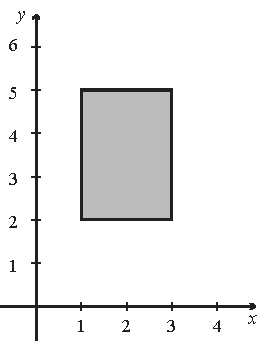
\includegraphics[width=\linewidth]{external/figps-cartprod.pdf}
\end{image}%
\tcblower
\end{figureptx}%
This illustrates that the graph of a Cartesian product of two intervals of finite length in \(\mathbb{R}\) corresponds to the interior of a rectangle and possibly some or all of its boundary. The solid line for the boundary in \hyperref[x:figure:fig_cartprod]{Figure~{\xreffont\ref{x:figure:fig_cartprod}}, p.\,\pageref{x:figure:fig_cartprod}} indicates that the boundary is included. In this case, the Cartesian product contained all of the boundary of the rectangle. When the graph does not contain a portion of the boundary, we usually draw that portion of the boundary with a dotted line.%
\par
Note: A Caution about Notation. The standard notation for an open interval in \(\mathbb{R}\) is the same as the notation for an ordered pair, which is an element of \textbackslash{}mbox\textbraceleft{}\(\mathbb{R} \times \mathbb{R}\)\textbraceright{} . We need to use the context in which the notation is used to determine which interpretation is intended. For example,%
\begin{itemize}[label=\textbullet]
\item{}If we write \(\left( {\sqrt 2 ,7} \right) \in \mathbb{R} \times \mathbb{R}\), then we are using \(\left( {\sqrt 2 ,7} \right)\) to represent an ordered pair of real numbers.%
\item{}If we write  \(\left( {1,2} \right) \times \left\{ 4 \right\}\), then we are interpreting  \(\left( {1,2} \right)\) as an open interval. We could write%
\begin{equation*}
\left( {1,2} \right) \times \left\{ 4 \right\} = \left\{ {\left. {\left( {x,4} \right)\,} \right|1 \lt  x \lt  2} \right\}\!\text{.}
\end{equation*}
%
\end{itemize}
%
\par
The following progress check explores some of the same ideas explored in \hyperref[x:exercise:prog_relationscartesian]{Progress Check~{\xreffont\ref{x:exercise:prog_relationscartesian}}, p.\,\pageref{x:exercise:prog_relationscartesian}} except that intervals of real numbers are used for the sets.%
\begin{inlineexercise}{Cartesian Products of Intervals.}{x:exercise:prog_cartprodintervals}%
\index{interval!Cartesian product}%
We will use the following intervals that are subsets of \(\R\).%
\begin{equation*}
A = \left[ {0,2} \right]  T = \left( {1,2} \right)  B = \left[ {2,4} \right)  
C = \left( {3,5} \right]
\end{equation*}
%
\begin{enumerate}[font=\bfseries,label=(\alph*),ref=\alph*]
\item\label{x:task:A_cartprodintervals1}Draw a graph of each of the following subsets of the Cartesian plane and write each subset using set builder notation.%
\begin{enumerate}[font=\bfseries,label=(\roman*),ref=\theenumi.\roman*]
\item{}\(A \times B\)%
\space\hyperlink{g:solution:idm822506280-back}{[Solution]}\item{}\(T \times B\)%
\space\hyperlink{g:solution:idm822504232-back}{[Solution]}\item{}\(A \times C\)%
\space\hyperlink{g:solution:idm822508840-back}{[Solution]}\item{}\(A \times \left( {B \cap C} \right)\)%
\space\hyperlink{g:solution:idm822499368-back}{[Solution]}\item{}\(\left( {A \times B} \right) \cap \left( {A \times C} \right)\)%
\space\hyperlink{g:solution:idm822502184-back}{[Solution]}\item{}\(A \times \left( {B \cup C} \right)\)%
\space\hyperlink{g:solution:idm822496424-back}{[Solution]}\item{}\(\left( {A \times B} \right) \cup \left( {A \times C} \right)\)%
\space\hyperlink{g:solution:idm822495912-back}{[Solution]}\item{}\(A \times \left( {B - C} \right)\)%
\space\hyperlink{g:solution:idm822501032-back}{[Solution]}\item{}\(\left( {A \times B} \right) - \left( {A \times C} \right)\)%
\space\hyperlink{g:solution:idm822491560-back}{[Solution]}\item{}\(B \times A\)%
\space\hyperlink{g:solution:idm822492200-back}{[Solution]}\end{enumerate}
\item{}List all the relationships between the sets in \hyperref[x:task:A_cartprodintervals1]{Task~{\xreffont\ref{x:exercise:prog_cartprodintervals}}.{\xreffont\ref{x:task:A_cartprodintervals1}}, p.\,\pageref{x:task:A_cartprodintervals1}} that you observe.%
\space\hyperlink{g:solution:idm822492072-back}{[Solution]}\end{enumerate}
\end{inlineexercise}%
One purpose of the work in \hyperref[x:exercise:prog_relationscartesian]{Progress Check~{\xreffont\ref{x:exercise:prog_relationscartesian}}, p.\,\pageref{x:exercise:prog_relationscartesian}} and \hyperref[x:exercise:prog_cartprodintervals]{Progress Check~{\xreffont\ref{x:exercise:prog_cartprodintervals}}, p.\,\pageref{x:exercise:prog_cartprodintervals}} was to indicate the plausibility of many of the results contained in the next theorem.%
\begin{theorem}{}{}{x:theorem:T_propsofcartprod}%
Let \(A\), \(B\), and \(C\) be sets. Then%
\begin{enumerate}
\item\label{x:li:T_propsofcartprod1}{}\hypertarget{x:li:T_propsofcartprod1}{}\(\displaystyle A \times \left( {B \cap C} \right) = \left( {A \times B} \right) \cap 
\left( {A \times C} \right)\)%
\item\label{x:li:T_propsofcartprod2}{}\hypertarget{x:li:T_propsofcartprod2}{}\(\displaystyle A \times \left( {B \cup C} \right) = \left( {A \times B} \right) \cup 
\left( {A \times C} \right)\)%
\item\label{x:li:T_propsofcartprod3}{}\hypertarget{x:li:T_propsofcartprod3}{}\(\displaystyle \left( {A \cap B} \right) \times C = \left( {A \times C} \right) \cap 
\left( {B \times C} \right)\)%
\item\label{x:li:T_propsofcartprod4}{}\hypertarget{x:li:T_propsofcartprod4}{}\(\displaystyle \left( {A \cup B} \right) \times C = \left( {A \times C} \right) \cup 
\left( {B \times C} \right)\)%
\item\label{x:li:T_propsofcartprod5}{}\hypertarget{x:li:T_propsofcartprod5}{}\(\displaystyle A \times \left( {B - C} \right) = \left( {A \times B} \right) - 
\left( {A \times C} \right)\)%
\item\label{x:li:T_propsofcartprod6}{}\hypertarget{x:li:T_propsofcartprod6}{}\(\displaystyle \left( {A - B} \right) \times C = \left( {A \times C} \right) - 
\left( {B \times C} \right)\)%
\item\label{x:li:T_propsofcartprod7}{}\hypertarget{x:li:T_propsofcartprod7}{}If \(T \subseteq A\), then \(T \times B \subseteq A \times B\).%
\item\label{x:li:T_propsofcartprod8}{}\hypertarget{x:li:T_propsofcartprod8}{}If \(Y \subseteq B\), then \(A \times Y \subseteq A \times B\).%
\end{enumerate}
%
\end{theorem}
We will not prove all these results; rather, we will prove \hyperlink{x:li:T_propsofcartprod2}{Item~{\xreffont 2}, p.\,\pageref{x:li:T_propsofcartprod2}} of \hyperref[x:theorem:T_propsofcartprod]{Theorem~{\xreffont\ref{x:theorem:T_propsofcartprod}}, p.\,\pageref{x:theorem:T_propsofcartprod}} and leave some of the rest to the exercises. In constructing these proofs, we need to keep in mind that Cartesian products are sets, and so we follow many of the same principles to prove set relationships that were introduced in \hyperref[x:section:S_provingset]{Section~{\xreffont\ref{x:section:S_provingset}}, p.\,\pageref{x:section:S_provingset}} and \hyperref[x:section:S_setproperties]{Section~{\xreffont\ref{x:section:S_setproperties}}, p.\,\pageref{x:section:S_setproperties}}.%
\par
The other thing to remember is that the elements of a Cartesian product are ordered pairs. So when we start a proof of a result such as \hyperlink{x:li:T_propsofcartprod2}{Item~{\xreffont 2}, p.\,\pageref{x:li:T_propsofcartprod2}} of \hyperref[x:theorem:T_propsofcartprod]{Theorem~{\xreffont\ref{x:theorem:T_propsofcartprod}}, p.\,\pageref{x:theorem:T_propsofcartprod}}, the primary goal is to prove that the two sets are equal. We will do this by proving that each one is a subset of the other one. So if we want to prove that \(A \times \left( {B \cup C} \right) \subseteq 
\left( {A \times B} \right) \cup \left( {A \times C} \right)\), we can start by choosing an arbitrary element of \(A \times \left( {B \cup C} \right)\). The goal is then to show that this element must be in \(\left( {A \times B} \right) \cup 
\left( {A \times C} \right)\). When we start by choosing an arbitrary element of \(A \times \left( {B \cup C} \right)\), we could give that element a name. For example, we could start by letting%
\begin{equation}
u \text{ be an element of }  A \times \left( {B \cup C} \right)\!\text{.}\label{x:men:eq_cartprod}
\end{equation}
We can then use the definition of ``ordered pair'' to conclude that%
\begin{equation}
\text{ there exists }  x \in A  \text{ and there exists }  y \in B \cup C 
\text{ such that }   u = \left( {x,y} \right)\text{.}\label{x:men:eq_cartprod2}
\end{equation}
In order to prove that \(A \times \left( {B \cup C} \right) \subseteq 
\left( {A \times B} \right) \cup \left( {A \times C} \right)\), we must now show that the ordered pair \(u\) from (1) is in \(\left( {A \times B} \right) \cup \left( {A \times C} \right)\). In order to do this, we can use the definition of set union and prove that%
\begin{equation}
u \in (A \times B) \text{ or }  u \in (A \times C)\text{.}\label{x:men:eq_cartprod3}
\end{equation}
Since \(u = (x, y)\), we can prove \hyperref[x:men:eq_cartprod3]{({\xreffont\ref{x:men:eq_cartprod3}})} by proving that%
\begin{equation}
\left( x \in A \text{ and }  y \in B \right) \text{ or }  \left( x \in A \text{ and }  y 
\in C \right)\text{.}\label{x:men:eq_cartprod4}
\end{equation}
%
\par
If we look at the sentences in \hyperref[x:men:eq_cartprod2]{({\xreffont\ref{x:men:eq_cartprod2}})} and \hyperref[x:men:eq_cartprod4]{({\xreffont\ref{x:men:eq_cartprod4}})}, it would seem that we are very close to proving that \(A \times \left( {B \cup C} \right) 
\subseteq \left( {A \times B} \right) \cup \left( {A \times C} \right)\). Following is a proof of \hyperlink{x:li:T_propsofcartprod2}{Item~{\xreffont 2}, p.\,\pageref{x:li:T_propsofcartprod2}} of \hyperref[x:theorem:T_propsofcartprod]{Theorem~{\xreffont\ref{x:theorem:T_propsofcartprod}}, p.\,\pageref{x:theorem:T_propsofcartprod}}.%
\begin{theorem}{Item~{\xreffont 2} of Theorem~{\xreffont\ref*{x:theorem:T_propsofcartprod}}.}{}{x:theorem:T_propsofcartprodx}%
Let \(A\), \(B\), and \(C\) be sets. Then%
\begin{equation*}
A \times \left( {B \cup C} \right) = \left( {A \times B} \right) \cup 
\left( {A \times C} \right)\text{.}
\end{equation*}
%
\end{theorem}
\begin{proof}{}{g:proof:idm822457256}
Let \(A\), \(B\), and \(C\) be sets. We will prove that \(A \times \left( {B \cup C} \right)\) is equal to \(\left( {A \times B} \right) \cup \left( {A \times C} \right)\) by proving that each set is a subset of the other set.%
\par
To prove that \(A \times \left( {B \cup C} \right) \subseteq \left( {A \times B} \right) 
\cup \left( {A \times C} \right)\), we let \(u \in A \times \left( {B \cup C} \right)\). Then there exists \(x \in A\) and there exists \(y \in B \cup C\) such that \(u = \left( {x,y} \right)\). Since \(y \in B \cup C\), we know that \(y \in B\) or \(y \in C\).%
\par
In the case where \(y \in B\), we have \(u = \left( {x,y} \right)\), where \(x \in A\) and \(y \in B\). So in this case, \(u \in A \times B\), and hence \(u \in \left( {A \times B} \right) \cup \left( {A \times C} \right)\). Similarly, in the case where \(y \in C\), we have \(u = \left( {x,y} \right)\), where \(x \in A\) and \(y \in C\). So in this case, \(u \in A \times C\) and, hence, \(u \in \left( {A \times B} \right) \cup \left( {A \times C} \right)\).%
\par
In both cases, \(u \in \left( {A \times B} \right) \cup \left( {A \times C} \right)\). Hence, we may conclude that if \(u\) is an element of \(A \times \left( {B \cup C} \right)\), then \(u \in \left( {A \times B} \right) \cup \left( {A \times C} \right)\), and this proves that%
\begin{equation}
A \times \left( {B \cup C} \right) \subseteq \left( {A \times B} \right) \cup 
\left( {A \times C} \right)\!\text{.}\label{x:men:eq_4m}
\end{equation}
%
\par
We must now prove that \(\left( {A \times B} \right) \cup \left( {A \times C} \right) 
\subseteq A \times \left( {B \cup C} \right)\). So we let \(v \in \left( {A \times B} \right) \cup \left( {A \times C} \right)\). Then \(v \in \left( {A \times B} \right)\) or \(v \in \left( {A \times C} \right)\).%
\par
In the case where \(v \in \left( {A \times B} \right)\), we know that there exists \(s \in A\) and there exists \(t \in B\) such that \(v = \left( {s,\;t} \right)\). But since \(t \in B\), we know that \(t \in B \cup C\), and hence \(v \in A \times \left( {B \cup C} \right)\). Similarly, in the case where \(v \in \left( {A \times C} \right)\), we know that there exists \(s \in A\) and there exists \(t \in C\) such that \(v = \left( {s,t} \right)\). But because \(t \in C\), we can conclude that \(t \in B \cup C\) and, hence, \(v \in A \times \left( {B \cup C} \right)\).%
\par
In both cases, \(v \in A \times \left( {B \cup C} \right)\). Hence, we may conclude that if%
\par
\(v \in \left( {A \times B} \right) \cup \left( {A \times C} \right)\), then \(v \in A \times \left( {B \cup C} \right)\), and this proves that%
\begin{equation}
\left( {A \times B} \right) \cup \left( {A \times C} \right) \subseteq A \times 
\left( {B \cup C} \right)\!\text{.}\label{x:men:eq_4n}
\end{equation}
%
\par
The relationships in \hyperref[x:men:eq_4m]{({\xreffont\ref{x:men:eq_4m}})} and \hyperref[x:men:eq_4n]{({\xreffont\ref{x:men:eq_4n}})} prove that \(A \times \left( {B \cup C} \right) = \left( {A \times B} \right) 
\cup \left( {A \times C} \right)\).%
\end{proof}
Final Note: The definition of an ordered pair in \hyperref[x:worksheet:PA_cartesianproduct]{Beginning Activity 2, p.\,\pageref{x:worksheet:PA_cartesianproduct}} may have seemed like a lengthy definition, but in some areas of mathematics, an even more formal and precise definition of ``ordered pair'' is needed. This definition is explored in \hyperref[x:activity:exer_defoforderedpair]{Activity~{\xreffont\ref{x:activity:exer_defoforderedpair}}, p.\,\pageref{x:activity:exer_defoforderedpair}}.%
\end{subsectionptx}
%
%
\typeout{************************************************}
\typeout{Exercises  Exercises}
\typeout{************************************************}
%
\begin{exercises-subsection}{Exercises}{}{Exercises}{}{}{g:exercises:idm822386472}
\begin{divisionexercise}{1}{}{}{x:exercise:exer_sec44-1}%
Let \(A = \left\{ {1,2} \right\}\), \(B = \left\{ {a,b,c,d} \right\}\), and \(C = \left\{ {1,a,b} \right\}\). Use the roster method to list all of the elements of each of the following sets:%
\begin{enumerate}[font=\bfseries,label=(\alph*),ref=\alph*]
\item{}\(A \times B\)%
\space\hyperlink{g:answer:idm822372648-back}{[Answer]}\item{}\(B \times A\)%
\space\hyperlink{g:answer:idm822372776-back}{[Answer]}\item{}\(A \times C\)%
\space\hyperlink{g:answer:idm822377128-back}{[Answer]}\item{}\(A^2\)%
\space\hyperlink{g:answer:idm822374312-back}{[Answer]}\item{}\(A \times \left( {B \cap C} \right)\)%
\space\hyperlink{g:answer:idm822370344-back}{[Answer]}\item{}\(\left( {A \times B} \right) \cap \left( {A \times C} \right)\)%
\space\hyperlink{g:answer:idm822367656-back}{[Answer]}\item{}\(A \times \emptyset\)%
\space\hyperlink{g:answer:idm822366376-back}{[Answer]}\item{}\(B \times \left\{ 2 \right\}\)%
\space\hyperlink{g:answer:idm822368808-back}{[Answer]}\end{enumerate}
\end{divisionexercise}%
\begin{divisionexercise}{2}{}{}{x:exercise:exer_sec44-2}%
Sketch a graph of each of the following Cartesian products in the Cartesian plane.%
\begin{enumerate}[font=\bfseries,label=(\alph*),ref=\alph*]
\item{}\(\left[ {0,2} \right] \times \left[ {1,3} \right]\)%
\item{}\(\left( {0,2} \right) \times \left( {1,3} \right]\)%
\item{}\(\left[ {2,3} \right] \times \left\{ 1 \right\}\)%
\item{}\(\left\{ 1 \right\} \times \left[ {2,3} \right]\)%
\item{}\(\mathbb{R} \times \left( {2,4} \right)\)%
\item{}\(\left( {2,4} \right) \times \mathbb{R}\)%
\item{}\(\mathbb{R} \times \left\{ { - 1} \right\}\)%
\item{}\(\left\{ { - 1} \right\} \times \left[ {1, + \infty } \right)\)%
\end{enumerate}
\end{divisionexercise}%
\begin{divisionexercise}{3}{}{}{x:exercise:exer_sec44-3}%
Prove \hyperref[x:theorem:T_propsofcartprod]{Theorem~{\xreffont\ref{x:theorem:T_propsofcartprod}}, p.\,\pageref{x:theorem:T_propsofcartprod}}, \hyperlink{x:li:T_propsofcartprod1}{Item~{\xreffont 1}, p.\,\pageref{x:li:T_propsofcartprod1}}: \(A \times \left( {B \cap C} \right) = \left( {A \times B} \right) \cap 
\left( {A \times C} \right)\).%
\space\hyperlink{g:answer:idm822358440-back}{[Answer]}\end{divisionexercise}%
\begin{divisionexercise}{4}{}{}{x:exercise:exer_sec44-4}%
Prove \hyperref[x:theorem:T_propsofcartprod]{Theorem~{\xreffont\ref{x:theorem:T_propsofcartprod}}, p.\,\pageref{x:theorem:T_propsofcartprod}}, \hyperlink{x:li:T_propsofcartprod4}{Item~{\xreffont 4}, p.\,\pageref{x:li:T_propsofcartprod4}}: \(\left( {A \cup B} \right) \times C = \left( {A \times C} \right) \cup 
\left( {B \times C} \right)\).%
\space\hyperlink{g:answer:idm822344360-back}{[Answer]}\end{divisionexercise}%
\begin{divisionexercise}{5}{}{}{g:exercise:idm822338344}%
Prove \hyperref[x:theorem:T_propsofcartprod]{Theorem~{\xreffont\ref{x:theorem:T_propsofcartprod}}, p.\,\pageref{x:theorem:T_propsofcartprod}}, \hyperlink{x:li:T_propsofcartprod5}{Item~{\xreffont 5}, p.\,\pageref{x:li:T_propsofcartprod5}}: \(A \times \left( {B - C} \right) = \left( {A \times B} \right) - 
\left( {A \times C} \right)\).%
\end{divisionexercise}%
\begin{divisionexercise}{6}{}{}{x:exercise:exer_sec44-6}%
Prove \hyperref[x:theorem:T_propsofcartprod]{Theorem~{\xreffont\ref{x:theorem:T_propsofcartprod}}, p.\,\pageref{x:theorem:T_propsofcartprod}}, \hyperlink{x:li:T_propsofcartprod7}{Item~{\xreffont 7}, p.\,\pageref{x:li:T_propsofcartprod7}}: If \(T \subseteq A\), then \(T \times B \subseteq A \times B\).%
\end{divisionexercise}%
\begin{divisionexercise}{7}{}{}{x:exercise:exer_sec44-7}%
Let \(A = \left\{ 1 \right\}\!, B = \left\{ 2 \right\}\!, \text{ and } 
C = \left\{ 3 \right\}\).%
\begin{enumerate}[font=\bfseries,label=(\alph*),ref=\alph*]
\item{}Explain why \(A \times B \ne B \times A\).%
\item{}Explain why \(\left( {A \times B} \right) \times C \ne A \times \left( {B \times C} 
\right)\).%
\end{enumerate}
\end{divisionexercise}%
\begin{divisionexercise}{8}{}{}{g:exercise:idm822333864}%
Let \(A\) and \(B\) be nonempty sets. Prove that \(A \times B = B \times A\) if and only if \(A = B\).%
\end{divisionexercise}%
\begin{divisionexercise}{9}{}{}{x:exercise:exer_sec44-9}%
Is the following proposition true or false? Justify your conclusion. \begin{quote}%
Let \(A\), \(B\), and \(C\) be sets with \(A \ne \emptyset\). If \(A \times B = A \times C\), then \(B = C\).\end{quote}
 Explain where the assumption that \(A \ne \emptyset\) is needed.%
\end{divisionexercise}%
\begin{activity}{A Set Theoretic Definition of an Ordered Pair.}{x:activity:exer_defoforderedpair}%
\index{Kuratowski, Kazimierz}%
\index{ordered pair}%
In elementary mathematics, the notion of an ordered pair introduced at the beginning of this section will suffice. However, if we are interested in a formal development of the Cartesian product of two sets, we need a more precise definition of ordered pair. Following is one way to do this in terms of sets. This definition is credited to Kazimierz Kuratowski (1896 \textemdash{} 1980). Kuratowski was a famous Polish mathematician whose main work was in the areas of topology and set theory. He was appointed the Director of the Polish Academy of Sciences and served in that position for 19 years. Let  \(x\)  be an element of the set  \(A\), and let  \(y\)  be an element of the set  \(B\). The \terminology{ordered pair} \(\left( {x,y} \right)\) is defined to be the set \(\left\{ {\left\{ x \right\},\left\{ {x,y} \right\}} \right\}\). That is,%
\begin{equation*}
\left( {x,y} \right) = \left\{ {\left\{ x \right\},\left\{ {x,y} \right\}} \right\}\!\text{.}
\end{equation*}
%
\begin{enumerate}[font=\bfseries,label=(\alph*),ref=\alph*]
\item{}Explain how this definition allows us to distinguish between the ordered pairs \(\left( {3,5} \right)\) and \(\left( {5,3} \right)\).%
\item{}\index{ordered triple}%
Let \(A\) and \(B\) be sets and let \(a,c \in A\) and \(b,d \in B\). Use this definition of an ordered pair and the concept of set equality to prove that \(\left( {a,b} \right) = \left( {c,d} \right)\) if and only if \(a = c\) and \(b = d\).%
\par
An \terminology{ordered triple} can be thought of as a single triple of objects, denoted by  \(\left( {a,b,c} \right)\), with an implied order.  This means that in order for two ordered triples to be equal, they must contain exactly the same objects in the same order.  That is, \(\left( {a,b,c} \right) = \left( {p,q,r} \right)\) if and only if  \(a = p\), \(b = q\) and \(c = r\).%
\item{}Let \(A\), \(B\), and \(C\) be sets, and let \(x \in A,y \in B,\text{ and } z \in C\). Write a set theoretic definition of the ordered triple \(\left( {x,y,z} \right)\) similar to the set theoretic definition of ``ordered pair.''%
\end{enumerate}
\end{activity}%
\end{exercises-subsection}
\end{sectionptx}
%
%
\typeout{************************************************}
\typeout{Section 5.5 Indexed Families of Sets}
\typeout{************************************************}
%
\begin{sectionptx}{Indexed Families of Sets}{}{Indexed Families of Sets}{}{}{x:section:S_indexfamily}
%
%
\typeout{************************************************}
\typeout{Beginning Activity  Beginning Activity 1: The Union and Intersection of a Family of Sets}
\typeout{************************************************}
%
\begin{worksheet-subsection}{Beginning Activity 1: The Union and Intersection of a Family of Sets}{}{Beginning Activity 1: The Union and Intersection of a Family of Sets}{}{}{x:worksheet:PA_foursets}
\begin{introduction}{}%
In \hyperref[x:section:S_setproperties]{Section~{\xreffont\ref{x:section:S_setproperties}}, p.\,\pageref{x:section:S_setproperties}}, we discussed various properties of set operations. We will now focus on the associative properties for set union and set intersection. Notice that the definition of ``set union'' tells us how to form the union of two sets. It is the associative law that allows us to discuss the union of three sets. Using the associate law, if \(A\), \(B\), and \(C\) are subsets of some universal set, then we can define \(A \cup B \cup C\) to be \(\left( A \cup B \right) \cup C\) or \(A \cup \left( B \cup C \right)\). That is,%
\begin{equation*}
A \cup B \cup C = \left(A \cup B \right) \cup C = A \cup \left( B \cup C \right)\!\text{.}
\end{equation*}
For this activity, the universal set is \(\N\) and we will use the following four sets:%
\begin{align*}
A \amp = \left\{ 1, 2, 3, 4, 5 \right\} \amp B \amp = \left\{ 2, 3, 4, 5, 6 \right\}\\
C \amp = \left\{ 3, 4, 5, 6, 7 \right\} \amp D \amp = \left\{ 4, 5, 6, 7, 8 \right\}
\end{align*}
%
\end{introduction}%
\begin{divisionexercise}{1}{}{}{x:exercise:PA_foursets1}%
Use the roster method to specify the sets \(A \cup B \cup C\), \(B \cup C \cup D\), \(A \cap B \cap C\), and \(B \cap C \cap D\).%
\end{divisionexercise}%
\begin{divisionexercise}{2}{}{}{x:exercise:PA_foursets2}%
Use the roster method to specify each of the following sets. In each case, be sure to follow the order specified by the parentheses.%
\begin{enumerate}[font=\bfseries,label=(\alph*),ref=\alph*]
\item{}\(\left( A \cup B \cup C \right) \cup D\)%
\item{}\(A \cup \left( B \cup C \cup D \right)\)%
\item{}\(A \cup \left( B \cup C \right) \cup D\)%
\item{}\(\left( A \cup B \right) \cup \left( C \cup D \right)\)%
\item{}\(\left( A \cap B \cap C \right) \cap D\)%
\item{}\(A \cap \left( B \cap C \cap D \right)\)%
\item{}\(A \cap \left( B \cap C \right) \cap D\)%
\item{}\(\left( A \cap B \right) \cap \left( C \cap D \right)\)%
\end{enumerate}
\end{divisionexercise}%
\begin{divisionexercise}{3}{}{}{x:exercise:PA_foursets3}%
Based on the work in \hyperlink{x:exercise:PA_foursets2}{Exercise~{\xreffont 2}, p.\,\pageref{x:exercise:PA_foursets2}}, does the placement of the parentheses matter when determining the union (or intersection) of these four sets? Does this make it possible to define \(A \cup B \cup C \cup D\) and \(A \cap B \cap C \cap D\)?%
\end{divisionexercise}%
\index{family of sets} We have already seen that the elements of a set may themselves be sets. For example, the power set of a set \(T\), \(\mathcal{P}( T )\), is the set of all subsets of \(T\). The phrase, ``a set of sets'' sounds confusing, and so we often use the terms \terminology{collection} and \terminology{family} when we wish to emphasize that the elements of a given set are themselves sets. We would then say that the power set of \(T\) is the family (or collection) of sets that are subsets of \(T\).%
\par
One of the purposes of the work we have done so far in this activity was to show that it is possible to define the union and intersection of a family of sets.%
\begin{assemblage}{Definition.}{x:assemblage:D_familyoper}%
\label{g:notation:idm822287016}\label{g:notation:idm822286376} Let \(\mathcal{C}\) be a family of sets. The \terminology{union of \(\mathbf{\mathcal{C}}\)} is defined as the set of all elements that are in at least one of the sets in \(\mathcal{C}\). We write%
\begin{equation*}
\bigcup_{X \in \mathscr{C}}^{}X = \left\{x \in U \mid x \in X \text{ for some }  X 
\in \mathscr{C} \right\}
\end{equation*}
%
\par
The \terminology{intersection of \(\mathbf{\mathcal{C}}\)} is defined as the set of all elements that are in all of the sets in \(\mathcal{C}\). That is,%
\begin{equation*}
\bigcap_{X \in \mathscr{C}}^{}X = \left\{x \in U \mid x \in X \text{ for all }  X 
\in \mathscr{C} \right\}
\end{equation*}
%
\end{assemblage}
For example, consider the four sets \(A\), \(B\), \(C\), and \(D\) used earlier in this activity and the sets%
\begin{equation*}
S = \left\{5, 6, 7, 8, 9 \right\}  \text{ and }   T = \left\{6, 7, 8, 9, 10 \right\}\text{.}
\end{equation*}
We can then consider the following families of sets: \(\mathscr{A} = \left\{A, B, C , D \right\}\) and \(\mathscr{B} = \left\{A, B, C , D, S, T \right\}\).%
\begin{divisionexercise}{4}{}{}{x:exercise:PA_foursets4}%
Explain why%
\begin{equation*}
\bigcup_{X \in \mathscr{A}}^{}X = A \cup B \cup C \cup D  \text{ and } 
\bigcap_{X \in \mathscr{A}}^{}X = A \cap B \cap C \cap D\text{,}
\end{equation*}
and use your work in \hyperlink{x:exercise:PA_foursets1}{Exercise~{\xreffont 1}, p.\,\pageref{x:exercise:PA_foursets1}}, \hyperlink{x:exercise:PA_foursets2}{Exercise~{\xreffont 2}, p.\,\pageref{x:exercise:PA_foursets2}}, and \hyperlink{x:exercise:PA_foursets3}{Exercise~{\xreffont 3}, p.\,\pageref{x:exercise:PA_foursets3}} to determine \(\bigcup\limits_{X \in \mathscr{A}}^{}X\) and \(\bigcap\limits_{X \in \mathscr{A}}^{}X\).%
\end{divisionexercise}%
\begin{divisionexercise}{5}{}{}{g:exercise:idm822265896}%
Use the roster method to specify \(\bigcup\limits_{X \in \mathscr{B}}^{}X\) and \(\bigcap\limits_{X \in \mathscr{B}}^{}X\).%
\end{divisionexercise}%
\begin{divisionexercise}{6}{}{}{g:exercise:idm822269992}%
Use the roster method to specify the sets \(\left( \bigcup\limits_{X \in \mathscr{A}}^{}X \right)^c\) and \(\bigcap\limits_{X \in \mathscr{A}}^{}X^c\). Remember that the universal set is \(\N\).%
\end{divisionexercise}%
\end{worksheet-subsection}
%
%
\typeout{************************************************}
\typeout{Beginning Activity  Beginning Activity 2: An Indexed Family of Sets}
\typeout{************************************************}
%
\begin{worksheet-subsection}{Beginning Activity 2: An Indexed Family of Sets}{}{Beginning Activity 2: An Indexed Family of Sets}{}{}{x:worksheet:PA_indexfamily}
We often use subscripts to identify sets. For example, in \hyperref[x:worksheet:PA_foursets]{Beginning Activity 1, p.\,\pageref{x:worksheet:PA_foursets}}, instead of using \(A\), \(B\), \(C\), and \(D\) as the names of the sets, we could have used \(A_1\), \(A_2\), \(A_3\), and \(A_4\). When we do this, we are using the subscript as an identifying tag, or index, for each set. We can also use this idea to specify an infinite family of sets. For example, for each natural number \(n\), we define%
\begin{equation*}
C_n = \left\{ n, n+1, n+2, n+3, n+4 \right\}\!\text{.}
\end{equation*}
So if we have a family of sets \(\mathscr{C} = \left\{ C_1, C_2, C_3, C_4 \right\}\), we use the notation \(\bigcup\limits_{j=1}^{4}C_j\) to mean the same thing as \(\bigcup\limits_{X \in \mathscr{C}}^{}X\).%
\begin{divisionexercise}{1}{}{}{g:exercise:idm822263848}%
Determine \(\bigcup\limits_{j=1}^{4}C_j\) and \(\bigcap\limits_{j=1}^{4}C_j\).%
\end{divisionexercise}%
We can see that with the use of subscripts, we do not even have to define the family of sets \(\mathscr{A}\). We can work with the infinite family of sets%
\begin{equation*}
\mathscr{C}^* = \left\{ A_n \mid n \in \N \right\}
\end{equation*}
and use the subscripts to indicate which sets to use in a union or an intersection.%
\begin{divisionexercise}{2}{}{}{g:exercise:idm822265384}%
Use the roster method to specify each of the following pairs of sets. The universal set is \(\N\).%
\begin{enumerate}[font=\bfseries,label=(\alph*),ref=\alph*]
\item{}\(\bigcup\limits_{j=1}^{6}C_j\) and \(\bigcap\limits_{j=1}^{6}C_j\)%
\item{}\(\bigcup\limits_{j=1}^{8}C_j\) and \(\bigcap\limits_{j=1}^{8}C_j\)%
\item{}\(\bigcup\limits_{j=4}^{8}C_j\) and \(\bigcap\limits_{j=4}^{8}C_j\)%
\item{}\(\left( \bigcap\limits_{j=1}^{4}C_j \right)^c\) and \(\bigcup\limits_{j=1}^{4}C_j^c\)%
\end{enumerate}
\end{divisionexercise}%
\end{worksheet-subsection}
%
%
\typeout{************************************************}
\typeout{Subsection  The Union and Intersection of an Indexed Family of Sets}
\typeout{************************************************}
%
\begin{subsectionptx}{The Union and Intersection of an Indexed Family of Sets}{}{The Union and Intersection of an Indexed Family of Sets}{}{}{x:subsection:sym_unionfiniteindex}
\label{g:notation:idm822250664}%
\label{g:notation:idm822256680}%
\label{g:notation:idm822252328}%
\label{g:notation:idm822250152}%
One of the purposes of the beginning activities was to show that we often encounter situations in which more than two sets are involved, and it is possible to define the union and intersection of more than two sets. In \hyperref[x:worksheet:PA_indexfamily]{Beginning Activity 2, p.\,\pageref{x:worksheet:PA_indexfamily}}, we also saw that it is often convenient to ``index'' the sets in a family of sets. In particular, if \(n\) is a natural number and \(\mathscr{A} = \left\{ A_1, A_2, \ldots , A_n \right\}\) is a family of \(n\) sets, then the union of these \(n\) sets, denoted by \(A_1 \cup A_2 \cup \cdots \cup A_n\) or \(\bigcup\limits_{j=1}^{n}A_j\), is defined as%
\begin{equation*}
\bigcup_{j=1}^{n}A_j = \left\{ x \in U \mid x \in A_j, \text{ for some }  j 
\text{ with }  1 \leq j \leq n \right\}\!\text{.}
\end{equation*}
We can also define the intersection of these \(n\) sets, denoted by \(A_1 \cap A_2 \cap \cdots \cap A_n\) or \(\bigcap\limits_{j=1}^{n}A_j\), as%
\begin{equation*}
\bigcap_{j=1}^{n}A_j = \left\{ x \in U \mid x \in A_j, \text{ for all }  j \text{ with }  1 \leq j \leq n \right\}\!\text{.}
\end{equation*}
We can also extend this idea to define the union and intersection of a family that consists of infinitely many sets. So if \(\mathscr{B} = \left\{ B_1, B_2, \ldots , B_n, \ldots \: \right\}\), then%
\begin{align*}
\bigcup_{j=1}^{\infty}B_j \amp = \left\{ x \in U \mid x \in B_j, 
\text{ for some }  j \text{ with }  j \geq 1 \right\}\!, \text{ and }\\
\bigcap_{j=1}^{\infty}B_j \amp = \left\{ x \in U \mid x \in B_j, 
\text{ for all }  j \text{ with }  j \geq 1 \right\}\!.
\end{align*}
%
\begin{inlineexercise}{An Infinite Family of Sets.}{x:exercise:prog_infinitefamily}%
For each natural number \(n\), let \(A_n = \left\{ 1, n, n^2 \right\}\). For example,%
\begin{equation*}
A_1 = \left\{ 1 \right\} \qquad A_2 = \left\{ 1, 2, 4 \right\} \qquad 
A_3 = \left\{ 1, 3, 9 \right\}\text{,}
\end{equation*}
and%
\begin{equation*}
\bigcup\limits_{j=1}^{3}A_j = \left\{1, 2, 3, 4, 9 \right\} \qquad
\bigcap\limits_{j=1}^{3}A_j = \left\{1 \right\}
\end{equation*}
%
\par
Determine each of the following sets:%
\begin{enumerate}[font=\bfseries,label=(\alph*),ref=\alph*]
\item{}\(\bigcup\limits_{j=1}^{6}A_j\)%
\space\hyperlink{g:solution:idm822247592-back}{[Solution]}\item{}\(\bigcap\limits_{j=1}^{6}A_j\)%
\space\hyperlink{g:solution:idm822236712-back}{[Solution]}\item{}\(\bigcup\limits_{j=3}^{6}A_j\)%
\space\hyperlink{g:solution:idm822233000-back}{[Solution]}\item{}\(\bigcap\limits_{j=3}^{6}A_j\)%
\space\hyperlink{g:solution:idm822233768-back}{[Solution]}\item{}\(\bigcup\limits_{j=1}^{\infty}A_j\)%
\space\hyperlink{g:solution:idm822240936-back}{[Solution]}\item{}\(\bigcap\limits_{j=1}^{\infty}A_j\)%
\space\hyperlink{g:solution:idm822235560-back}{[Solution]}\end{enumerate}
\end{inlineexercise}%
In all of the examples we have studied so far, we have used \(\N\) or a subset of \(\N\) to index or label the sets in a family of sets. We can use other sets to index or label sets in a family of sets. For example, for each real number \(x\), we can define \(B_x\) to be the closed interval \(\left[x, x + 2 \right]\). That is,%
\begin{equation*}
B_x = \left\{ y \in \R \mid x \leq y \leq x + 2 \right\}\text{.}
\end{equation*}
So we make the following definition. In this definition, \(\Lambda\) is the uppercase Greek letter lambda and \(\alpha\) is the lowercase Greek letter alpha.%
\begin{assemblage}{Definition.}{x:assemblage:D_indexfamily}%
\label{g:notation:idm822227752} Let \(\Lambda\) be a nonempty set and suppose that for each \(\alpha \in \Lambda\), there is a corresponding set \(A_\alpha\). The family of sets \(\left\{ A_\alpha \mid \alpha \in \Lambda \right\}\) is called an \terminology{indexed family of sets} indexed by \(\Lambda\). Each \(\alpha \in \Lambda\) is called an \terminology{index} and \(\Lambda\) is called an \terminology{indexing set}.%
\end{assemblage}
\begin{inlineexercise}{Indexed Families of Sets.}{x:exercise:prog_indexfamily}%
In each of the indexed families of sets that we seen so far, if the indices were different, then the sets were different. That is, if \(\Lambda\) is an indexing set for the family of sets \(\mathscr{A} = \left\{ A_\alpha \mid \alpha \in \Lambda \right\}\), then if \(\alpha, \beta \in \Lambda\) and \(\alpha \ne \beta\), then \(A_\alpha \ne A_\beta\). (Note: The letter \(\beta\) is the Greek lowercase beta.)%
\begin{enumerate}[font=\bfseries,label=(\alph*),ref=\alph*]
\item{}Let \(\Lambda = \left\{ 1, 2, 3, 4 \right\}\), and for each \(n \in \Lambda\), let \(A_n = \left\{ 2n + 6, 16 - 2n \right\}\), and let \(\mathscr{A} = \left\{A_1, A_2, A_3, A_4 \right\}\). Determine \(A_1\), \(A_2\), \(A_3\), and \(A_4\).%
\space\hyperlink{g:solution:idm822213160-back}{[Solution]}\item{}Is the following statement true or false for the indexed family \(\mathscr{A}\) in~(1)? \begin{quote}%
For all \(m, n \in \Lambda\), if \(m \ne n\), then \(A_m \ne A_n\).\end{quote}
%
\space\hyperlink{g:solution:idm822214824-back}{[Solution]}\item{}Now let \(\Lambda = \R\). For each \(x \in \R\), define \(B_x = \left\{ 0, x^2, x^4 \right\}\). Is the following statement true for the indexed family of sets \(\mathscr{B} = \left\{ B_x \mid x \in \R \right\}\)? \begin{quote}%
For all \(x, y \in \R\), if \(x \ne y\), then \(B_x \ne B_y\).\end{quote}
%
\space\hyperlink{g:solution:idm822205864-back}{[Solution]}\end{enumerate}
\end{inlineexercise}%
We now restate the definitions of the union and intersection of a family of sets for an indexed family of sets.%
\begin{assemblage}{Definition.}{x:assemblage:D_indexoper}%
\label{g:notation:idm822204712}\label{g:notation:idm822203944} Let \(\Lambda\) be a nonempty indexing set and let \(\mathscr{A} = \left\{ A_\alpha \mid \alpha \in \Lambda \right\}\) be an indexed family of sets. The \terminology{union over} \(\mathbf{\mathscr{A}}\) is defined as the set of all elements that are in at least one of sets \(A_\alpha\), where \(\alpha \in \Lambda\). We write%
\begin{equation*}
\bigcup_{\alpha \in \Lambda}^{}A_\alpha = \left\{ x \in U \mid \text{ there exists an } 
\alpha \in \Lambda \text{ with }  x \in A_\alpha \right\}\!\text{.}
\end{equation*}
%
\par
The \terminology{intersection over} \(\mathbf{\mathscr{A}}\) is the set of all elements that are in all of the sets \(A_\alpha\) for each \(\alpha \in \Lambda\). That is,%
\begin{equation*}
\bigcap_{\alpha \in \Lambda}^{}A_\alpha = \left\{ x \in U \mid \text{ for all } 
\alpha \in \Lambda,  x \in A_\alpha \right\}\!\text{.}
\end{equation*}
%
\end{assemblage}
\begin{example}{A Family of Sets Indexed by the Positive Real Numbers.}{x:example:exam_indexfamily}%
For each positive real number \(\alpha\), let \(A_\alpha\) be the interval \(\left( -1, \alpha \right]\). That is,%
\begin{equation*}
A_\alpha = \left\{ x \in \R \mid -1 \lt  x \leq \alpha \right\}\!\text{.}
\end{equation*}
%
\par
If we let \(\R^+\) be the set of positive real numbers, then we have a family of sets indexed by \(\R^+\). We will first determine the union of this family of sets. Notice that for each \(\alpha \in \R^+\), \(\alpha \in A_\alpha\), and if \(y\) is a real number with \(-1 \lt  y \leq 0\), then \(y \in A_\alpha\). Also notice that if \(y \in \R\) and \(y \lt  -1\), then for each \(\alpha \in \R^+\), \(y \notin A_\alpha\). With these observations, we conclude that%
\begin{equation*}
\bigcup_{\alpha \in \R^+}^{}A_\alpha = \left( -1, \infty \right) = 
\left\{ x \in \R \mid -1 \lt  x \right\}\!\text{.}
\end{equation*}
%
\par
To determine the intersection of this family, notice that%
\begin{itemize}[label=\textbullet]
\item{}if \(y \in \R\) and \(y \lt -1\), then for each \(\alpha \in \R^+\), \(y \notin A_\alpha\);%
\item{}if \(y \in \R\) and \(-1 \lt y \leq 0\), then \(y \in A_\alpha\) for each \(\alpha \in \R^+\); and%
\item{}if \(y \in \R\) and \(y > 0\), then if we let \(\beta = \dfrac{y}{2}\), \(y > \beta\) and \(y \notin A_\beta\).%
\end{itemize}
%
\par
From these observations, we conclude that%
\begin{equation*}
\bigcap_{\alpha \in \R^+}^{}A_\alpha = \left( -1, 0 \right] = 
\left\{ x \in \R \mid -1 \lt  x \leq 0 \right\}\!\text{.}
\end{equation*}
%
\end{example}
\begin{inlineexercise}{A Continuation of Example~{\xreffont\ref*{x:example:exam_indexfamily}}.}{x:exercise:prog_indexfamily2}%
Using the family of sets from \hyperref[x:example:exam_indexfamily]{Example~{\xreffont\ref{x:example:exam_indexfamily}}, p.\,\pageref{x:example:exam_indexfamily}}, for each \(\alpha \in \R^+\), we see that%
\begin{equation*}
A_{\alpha}^c = \left(-\infty, -1 \right] \cup \left( \alpha, \infty \right)\!\text{.}
\end{equation*}
Use the results from \hyperref[x:example:exam_indexfamily]{Example~{\xreffont\ref{x:example:exam_indexfamily}}, p.\,\pageref{x:example:exam_indexfamily}} to help determine each of the following sets. For each set, use either interval notation or set builder notation.%
\begin{enumerate}[font=\bfseries,label=(\alph*),ref=\alph*]
\item{}\(\left( \bigcup\limits_{\alpha \in \R^+}^{}A_\alpha \right)^c\)%
\space\hyperlink{g:solution:idm822176168-back}{[Solution]}\item{}\(\bigcap\limits_{\alpha \in \R^+}^{}A_{\alpha}^c\)%
\space\hyperlink{g:solution:idm822172584-back}{[Solution]}\item{}\(\left( \bigcap\limits_{\alpha \in \R^+}^{}A_\alpha \right)^c\)%
\space\hyperlink{g:solution:idm822172328-back}{[Solution]}\item{}\(\bigcup\limits_{\alpha \in \R^+}^{}A_{\alpha}^c\)%
\space\hyperlink{g:solution:idm822170664-back}{[Solution]}\end{enumerate}
\end{inlineexercise}%
\end{subsectionptx}
%
%
\typeout{************************************************}
\typeout{Subsection  Properties of Union and Intersection}
\typeout{************************************************}
%
\begin{subsectionptx}{Properties of Union and Intersection}{}{Properties of Union and Intersection}{}{}{g:subsection:idm822168232}
In \hyperref[x:theorem:T_indexproperties]{Theorem~{\xreffont\ref{x:theorem:T_indexproperties}}, p.\,\pageref{x:theorem:T_indexproperties}}, we will prove some properties of set operations for indexed families of sets. Some of these properties are direct extensions of corresponding properties for two sets. For example, we have already proved De Morgan's Laws for two sets in \hyperref[x:theorem:T_propsofcomplements]{Theorem~{\xreffont\ref{x:theorem:T_propsofcomplements}}, p.\,\pageref{x:theorem:T_propsofcomplements}}. The work in the beginning activities and \hyperref[x:exercise:prog_indexfamily2]{Progress Check~{\xreffont\ref{x:exercise:prog_indexfamily2}}, p.\,\pageref{x:exercise:prog_indexfamily2}} suggests that we should get similar results using set operations with an indexed family of sets. For example, in \hyperref[x:worksheet:PA_indexfamily]{Beginning Activity 2, p.\,\pageref{x:worksheet:PA_indexfamily}}, we saw that%
\begin{equation*}
\left( \bigcap_{j=1}^{4}A_j \right)^c = \bigcup_{j=1}^{4}A_j^c\text{.}
\end{equation*}
%
\begin{theorem}{}{}{x:theorem:T_indexproperties}%
Let \(\Lambda\) be a nonempty indexing set and let \(\mathscr{A} = \left\{ A_\alpha \mid \alpha \in \Lambda \right\}\) be an indexed family of sets, each of which is a subset of some universal set \(U\). Then%
\begin{enumerate}
\item\label{x:li:T_indexproperties1}{}\hypertarget{x:li:T_indexproperties1}{}For each \(\beta \in \Lambda\), \(\bigcap\limits_{\alpha \in \Lambda}^{}A_\alpha \subseteq A_\beta\).%
\item\label{x:li:T_indexproperties2}{}\hypertarget{x:li:T_indexproperties2}{}For each \(\beta \in \Lambda\), \(A_\beta \subseteq \bigcup\limits_{\alpha \in \Lambda}^{}A_\alpha\).%
\item\label{x:li:T_indexproperties3}{}\hypertarget{x:li:T_indexproperties3}{}\(\displaystyle \left(\:\bigcap\limits_{\alpha \in \Lambda}^{}A_\alpha \right)^c = 
\bigcup\limits_{\alpha \in \Lambda}^{}A_{\alpha}^c\)%
\item\label{x:li:T_indexproperties4}{}\hypertarget{x:li:T_indexproperties4}{}\(\displaystyle \left(\:\bigcup\limits_{\alpha \in \Lambda}^{}A_\alpha \right)^c = 
\bigcap\limits_{\alpha \in \Lambda}^{}A_{\alpha}^c\)%
\end{enumerate}
%
\par
\index{De Morgan's Laws!for indexed family of sets}\index{indexed family of sets!De Morgan's Laws} \hyperlink{x:li:T_indexproperties3}{Item~{\xreffont 3}, p.\,\pageref{x:li:T_indexproperties3}} and \hyperlink{x:li:T_indexproperties4}{Item~{\xreffont 4}, p.\,\pageref{x:li:T_indexproperties4}} are known as \terminology{De Morgan's Laws}.%
\end{theorem}
\begin{proof}{}{g:proof:idm822152104}
We will prove \hyperlink{x:li:T_indexproperties1}{Item~{\xreffont 1}, p.\,\pageref{x:li:T_indexproperties1}} and \hyperlink{x:li:T_indexproperties3}{Item~{\xreffont 3}, p.\,\pageref{x:li:T_indexproperties3}}. The proofs of \hyperlink{x:li:T_indexproperties2}{Item~{\xreffont 2}, p.\,\pageref{x:li:T_indexproperties2}} and \hyperlink{x:li:T_indexproperties4}{Item~{\xreffont 4}, p.\,\pageref{x:li:T_indexproperties4}} are included in \hyperlink{x:exercise:exer_indexproperties}{Exercise~{\xreffont 4}, p.\,\pageref{x:exercise:exer_indexproperties}}. So we let \(\Lambda\) be a nonempty indexing set and let \(\mathscr{A} = \left\{ A_\alpha \mid \alpha \in \Lambda \right\}\) be an indexed family of sets. To prove \hyperlink{x:li:T_indexproperties1}{Item~{\xreffont 1}, p.\,\pageref{x:li:T_indexproperties1}}, we let \(\beta \in \Lambda\) and note that if \(x \in \bigcap\limits_{\alpha \in \Lambda}^{}A_\alpha\), then \(x \in A_\alpha\), for all \(\alpha \in \Lambda\). Since \(\beta\) is one element in \(\Lambda\), we may conclude that \(x \in A_\beta\). This proves that \(\bigcap\limits_{\alpha \in \Lambda}^{}A_\alpha \subseteq A_\beta\).%
\par
To prove \hyperlink{x:li:T_indexproperties3}{Item~{\xreffont 3}, p.\,\pageref{x:li:T_indexproperties3}}, we will prove that each set is a subset of the other set. We first let \(x \in \left(\:\bigcap\limits_{\alpha \in \Lambda}^{}A_\alpha \right)^c\). This means that \(x \notin \left(\:\bigcap\limits_{\alpha \in \Lambda}^{}A_\alpha \right)\), and this means that \begin{quote}%
there exists a \(\beta \in \Lambda\) such that \(x \notin A_\beta\).\end{quote}
 Hence, \(x \in A_{\beta}^c\), which implies that \(x \in \bigcup\limits_{\alpha \in \Lambda}^{}A_{\alpha}^c\). Therefore, we have proved that%
\begin{equation}
\left(\:\bigcap_{\alpha \in \Lambda}^{}A_\alpha \right)^c \subseteq 
\bigcup_{\alpha \in \Lambda}^{}A_{\alpha}^c\text{.}\label{x:men:eq_indexproperties1}
\end{equation}
%
\par
We now let \(y \in \bigcup\limits_{\alpha \in \Lambda}^{}A_{\alpha}^c\). This means that there exists a \(\beta \in \Lambda\) such that \(y \in A_{\beta}^c\) or \(y \notin A_\beta\). However, since \(y \notin A_\beta\), we may conclude that \(y \notin \bigcap\limits_{\alpha \in \Lambda}^{}A_\alpha\) and, hence, \(y \in \left(\:\bigcap\limits_{\alpha \in \Lambda}^{}A_\alpha \right)^c\). This proves that%
\begin{equation}
\bigcup_{\alpha \in \Lambda}^{}A_{\alpha}^c \subseteq 
\left(\:\bigcap_{\alpha \in \Lambda}^{}A_\alpha \right)^c\text{.}\label{x:men:eq_indexproperties2}
\end{equation}
%
\par
Using the results in \hyperref[x:men:eq_indexproperties1]{({\xreffont\ref{x:men:eq_indexproperties1}})} and \hyperref[x:men:eq_indexproperties2]{({\xreffont\ref{x:men:eq_indexproperties2}})}, we have proved that \(\left(\:\bigcap\limits_{\alpha \in \Lambda}^{}A_\alpha \right)^c = 
\bigcup\limits_{\alpha \in \Lambda}^{}A_{\alpha}^c\).%
\end{proof}
\index{distributive laws!for indexed family of sets}\index{indexed family of sets!distributive laws} Many of the other properties of set operations are also true for indexed families of sets. \hyperref[x:theorem:T_distributeindex]{Theorem~{\xreffont\ref{x:theorem:T_distributeindex}}, p.\,\pageref{x:theorem:T_distributeindex}} states the \terminology{distributive laws} for set operations.%
\begin{theorem}{}{}{x:theorem:T_distributeindex}%
Let \(\Lambda\) be a nonempty indexing set, let \(\mathscr{A} = \left\{ A_\alpha \mid \alpha \in \Lambda \right\}\) be an indexed family of sets, and let \(B\) be a set. Then%
\begin{enumerate}
\item{}\(B \cap \left(\:\bigcup\limits_{\alpha \in \Lambda}^{}A_{\alpha} \right) = 
\bigcup\limits_{\alpha \in \Lambda}^{} \left( B \cap A_{\alpha} \right)\), and%
\item{}\(B \cup \left(\:\bigcap\limits_{\alpha \in \Lambda}^{}A_{\alpha} \right) = 
\bigcap\limits_{\alpha \in \Lambda}^{} \left( B \cup A_{\alpha} \right)\).%
\end{enumerate}
%
\end{theorem}
The proof of \hyperref[x:theorem:T_distributeindex]{Theorem~{\xreffont\ref{x:theorem:T_distributeindex}}, p.\,\pageref{x:theorem:T_distributeindex}} is \hyperlink{x:exercise:exer_distributeindex}{Exercise~{\xreffont 5}, p.\,\pageref{x:exercise:exer_distributeindex}}.%
\end{subsectionptx}
%
%
\typeout{************************************************}
\typeout{Subsection  Pairwise Disjoint Families of Sets}
\typeout{************************************************}
%
\begin{subsectionptx}{Pairwise Disjoint Families of Sets}{}{Pairwise Disjoint Families of Sets}{}{}{g:subsection:idm822401704}
In \hyperref[x:section:S_provingset]{Section~{\xreffont\ref{x:section:S_provingset}}, p.\,\pageref{x:section:S_provingset}}, we defined two sets \(A\) and \(B\) to be disjoint provided that \(A \cap B = \emptyset\). In a similar manner, if \(\Lambda\) is a nonempty indexing set and \(\mathscr{A} = \left\{ A_\alpha \mid \alpha \in \Lambda \right\}\) is an indexed family of sets, we can say that this indexed family of sets is \terminology{disjoint} provided that \(\bigcap\limits_{\alpha \in \Lambda}^{}A_\alpha = \emptyset\). However, we can use the concept of two disjoint sets to define a somewhat more interesting type of ``disjointness'' for an indexed family of sets.%
\begin{assemblage}{Definition.}{x:assemblage:D_disjointfamily}%
Let \(\Lambda\) be a nonempty indexing set, and let \(\mathscr{A} = \left\{ A_\alpha \mid \alpha \in \Lambda \right\}\) be an indexed family of sets. We say that \(\mathscr{A}\) is \terminology{pairwise disjoint} provided that for all \(\alpha\) and \(\beta\) in \(\Lambda\), if \(A_\alpha \ne A_\beta\), then \(A_\alpha \cap A_\beta = \emptyset\).%
\end{assemblage}
\begin{inlineexercise}{Disjoint Families of Sets.}{x:exercise:prog_disjoint}%
\hyperref[x:figure:fig_disjoint]{Figure~{\xreffont\ref{x:figure:fig_disjoint}}, p.\,\pageref{x:figure:fig_disjoint}} shows two families of sets,%
\begin{equation*}
\mathscr{A} = \left\{A_1, A_2, A_3, A_4 \right\} \text{ and }
\mathscr{B} = \left\{B_1, B_2, B_3, B_4 \right\}
\end{equation*}
%
\begin{figureptx}{Two Families of Indexed Sets}{x:figure:fig_disjoint}{}%
\begin{image}{0.125}{0.75}{0.125}%
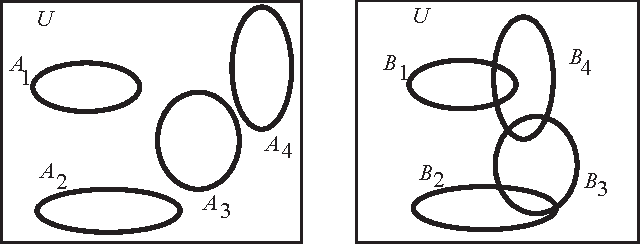
\includegraphics[width=\linewidth]{external/figps-disjoint.pdf}
\end{image}%
One figure has four sets, A1 to A4. No sets overlap. The second figure has four sets, B1 to B4. B1 and B4 overlap, B2 and B3 overlap, and B3 and B4 overlap.\tcblower
\end{figureptx}%
\begin{enumerate}[font=\bfseries,label=(\alph*),ref=\alph*]
\item{}Is the family of sets \(\mathscr{A}\) a disjoint family of sets? A pairwise disjoint family of sets?%
\item{}Is the family of sets \(\mathscr{B}\) a disjoint family of sets? A pairwise disjoint family of sets?%
\item{}Now let the universal set be \(\R\). For each \(n \in \N\), let \(C_n = \left( n, \infty \right)\), and let \(\mathscr{C} = \left\{ C_n \mid n \in \N \right\}\).%
\par
Is the family of sets \(\mathscr{C}\) a disjoint family of sets? A pairwise disjoint family of sets?%
\space\hyperlink{g:solution:idm822117144-back}{[Solution]}\end{enumerate}
\end{inlineexercise}%
\end{subsectionptx}
%
%
\typeout{************************************************}
\typeout{Exercises  Exercises}
\typeout{************************************************}
%
\begin{exercises-subsection}{Exercises}{}{Exercises}{}{}{g:exercises:idm822112792}
\begin{divisionexercise}{1}{}{}{x:exercise:exer_sec45-example1}%
For each natural number \(n\), let \(A_n = \left\{n, n+1, n+2, n+3 \right\}\). Use the roster method to specify each of the following sets:%
\begin{enumerate}[font=\bfseries,label=(\alph*),ref=\alph*]
\item{}\(\bigcap\limits_{j=1}^{3}A_j\)%
\space\hyperlink{g:answer:idm822107672-back}{[Answer]}\item{}\(\bigcup\limits_{j=1}^{3}A_j\)%
\item{}\(\bigcap\limits_{j=3}^{7}A_j\)%
\item{}\(\bigcup\limits_{j=3}^{7}A_j\)%
\space\hyperlink{g:answer:idm822107288-back}{[Answer]}\item{}\(A_9 \cap \left(\:\bigcup\limits_{j=3}^{7}A_j \right)\)%
\item{}\(\bigcup\limits_{j=3}^{7}\left( A_9 \cap A_j \right)\)%
\end{enumerate}
\end{divisionexercise}%
\begin{divisionexercise}{2}{}{}{x:exercise:exer_sec45-example2}%
For each natural number \(n\), let \(A_n = \left\{ k \in \N \left| \hspace{3pt} k \geq n \right. \right\}\). Assuming the universal set is \(\N\), use the roster method or set builder notation to specify each of the following sets:%
\begin{enumerate}[font=\bfseries,label=(\alph*),ref=\alph*]
\item{}\(\bigcap\limits_{j=1}^{5}A_j\)%
\space\hyperlink{g:answer:idm822099352-back}{[Answer]}\item{}\(\left(\: \bigcap\limits_{j=1}^{5}A_j \right)^c\)%
\item{}\(\bigcap\limits_{j=1}^{5}A_j^c\)%
\space\hyperlink{g:answer:idm822094232-back}{[Answer]}\item{}\(\bigcup\limits_{j=1}^{5}A_j^c\)%
\space\hyperlink{g:answer:idm822101528-back}{[Answer]}\item{}\(\bigcup\limits_{j=1}^{5}A_j\)%
\item{}\(\left(\: \bigcup\limits_{j=1}^{5}A_j \right)^c\)%
\space\hyperlink{g:answer:idm822099608-back}{[Answer]}\item{}\(\bigcap\limits_{j \in \N}^{}A_j\)%
\item{}\(\bigcup\limits_{j \in \N}^{}A_j\)%
\end{enumerate}
\end{divisionexercise}%
\begin{divisionexercise}{3}{}{}{x:exercise:exer_indexpositivereals}%
For each positive real number \(r\), define \(T_r\) to be the closed interval \(\left[ -r^2, r^2 \right]\). That is,%
\begin{equation*}
T_r = \left\{ x \in \R \left| -r^2 \leq x \leq r^2 \right. \right\}\!\text{.}
\end{equation*}
Let \(\Lambda = \left\{ m \in \N \left| 1 \leq m \leq 10 \right. \right\}\). Use either interval notation or set builder notation to specify each of the following sets:%
\begin{enumerate}[font=\bfseries,label=(\alph*),ref=\alph*]
\item{}\(\bigcup\limits_{k \in \Lambda}^{}T_k\)%
\space\hyperlink{g:answer:idm822089880-back}{[Answer]}\item{}\(\bigcap\limits_{k \in \Lambda}^{}T_k\)%
\space\hyperlink{g:answer:idm822091672-back}{[Answer]}\item{}\(\bigcup\limits_{r \in \R^+}^{}T_r\)%
\item{}\(\bigcap\limits_{r \in \R^+}^{}T_r\)%
\item{}\(\bigcup\limits_{k \in \N}^{}T_k\)%
\item{}\(\bigcap\limits_{k \in \N}^{}T_k\)%
\end{enumerate}
\end{divisionexercise}%
\begin{divisionexercise}{4}{}{}{x:exercise:exer_indexproperties}%
Prove \hyperlink{x:li:T_indexproperties2}{Item~{\xreffont 2}, p.\,\pageref{x:li:T_indexproperties2}} and~\hyperlink{x:li:T_indexproperties4}{Item~{\xreffont 4}, p.\,\pageref{x:li:T_indexproperties4}} of \hyperref[x:theorem:T_indexproperties]{Theorem~{\xreffont\ref{x:theorem:T_indexproperties}}, p.\,\pageref{x:theorem:T_indexproperties}}. Let \(\Lambda\) be a nonempty indexing set and let \(\mathscr{A} = \left\{ A_\alpha \mid \alpha \in \Lambda \right\}\) be an indexed family of sets.%
\begin{enumerate}[font=\bfseries,label=(\alph*),ref=\alph*]
\item{}For each \(\beta \in \Lambda\), \(A_\beta \subseteq \bigcup\limits_{\alpha \in \Lambda}^{}A_\alpha\).%
\space\hyperlink{g:answer:idm822079128-back}{[Answer]}\item{}\(\left(\:\bigcup\limits_{\alpha \in \Lambda}^{}A_\alpha \right)^c = 
\bigcap\limits_{\alpha \in \Lambda}^{}A_{\alpha}^c\)%
\end{enumerate}
\end{divisionexercise}%
\begin{divisionexercise}{5}{}{}{x:exercise:exer_distributeindex}%
Prove \hyperref[x:theorem:T_distributeindex]{Theorem~{\xreffont\ref{x:theorem:T_distributeindex}}, p.\,\pageref{x:theorem:T_distributeindex}}. Let \(\Lambda\) be a nonempty indexing set, let \(\mathscr{A} = \left\{ A_\alpha \mid \alpha \in \Lambda \right\}\) be an indexed family of sets, and let \(B\) be a set. Then%
\begin{enumerate}[font=\bfseries,label=(\alph*),ref=\alph*]
\item{}\(B \cap \left(\:\bigcup\limits_{\alpha \in \Lambda}^{}A_{\alpha} \right) = 
\bigcup\limits_{\alpha \in \Lambda}^{} \left( B \cap A_{\alpha} \right)\), and%
\space\hyperlink{g:answer:idm822072600-back}{[Answer]}\item{}\(B \cup \left(\:\bigcap\limits_{\alpha \in \Lambda}^{}A_{\alpha} \right) = 
\bigcap\limits_{\alpha \in \Lambda}^{} \left( B \cup A_{\alpha} \right)\).%
\end{enumerate}
\end{divisionexercise}%
\begin{divisionexercise}{6}{}{}{x:exercise:exer_doubledistribute}%
Let \(\Lambda\) and \(\Gamma\) be nonempty indexing sets. (Note: The letter \(\Gamma\) is the uppercase Greek letter gamma.) Also, let \(\mathscr{A} = \left\{ A_\alpha \mid \alpha \in \Lambda \right\}\) and \(\mathscr{B} = \left\{ B_\beta \mid \beta \in \Gamma \right\}\) be indexed families of sets. Use the distributive laws in \hyperlink{x:exercise:exer_distributeindex}{Exercise~{\xreffont 5}, p.\,\pageref{x:exercise:exer_distributeindex}} to:%
\begin{enumerate}[font=\bfseries,label=(\alph*),ref=\alph*]
\item{}Write \(\left(\: \bigcup\limits_{\alpha \in \Lambda}^{}A_\alpha\right) \cap 
\left(\: \bigcup\limits_{\beta \in \Gamma}^{}B_\beta \right)\) as a union of intersections of two sets.%
\item{}Write \(\left(\: \bigcap\limits_{\alpha \in \Lambda}^{}A_\alpha\right) \cup 
\left(\: \bigcap\limits_{\beta \in \Gamma}^{}B_\beta \right)\) as an intersection of unions of two sets.%
\end{enumerate}
\end{divisionexercise}%
\begin{divisionexercise}{7}{}{}{g:exercise:idm822059800}%
Let \(\Lambda\) be a nonempty indexing set and let \(\mathscr{A} = \left\{ A_\alpha \mid \alpha \in \Lambda \right\}\) be an indexed family of sets. Also, assume that \(\Gamma \subseteq \Lambda\) and \(\Gamma \ne \emptyset\). Prove that%
\begin{enumerate}[font=\bfseries,label=(\alph*),ref=\alph*]
\item{}\(\bigcup\limits_{\alpha \in \Gamma}^{}A_\alpha \subseteq 
\bigcup\limits_{\alpha \in \Lambda}^{}A_\alpha\)%
\item{}\(\bigcap\limits_{\alpha \in \Lambda}^{}A_\alpha \subseteq 
\bigcap\limits_{\alpha \in \Gamma}^{}A_\alpha\)%
\end{enumerate}
\end{divisionexercise}%
\begin{divisionexercise}{8}{}{}{x:exercise:exer_indexsubsets}%
Let \(\Lambda\) be a nonempty indexing set and let \(\mathscr{A} = \left\{ A_\alpha \mid \alpha \in \Lambda \right\}\) be an indexed family of sets.%
\begin{enumerate}[font=\bfseries,label=(\alph*),ref=\alph*]
\item{}Prove that if \(B\) is a set such that \(B \subseteq A_\alpha\) for every \(\alpha \in \Lambda\), then \(B \subseteq \bigcap\limits_{\alpha \in \Lambda}^{}A_\alpha\).%
\space\hyperlink{g:answer:idm822051608-back}{[Answer]}\item{}Prove that if \(C\) is a set such that \(A_\alpha \subseteq C\) for every \(\alpha \in \Lambda\), then \(\bigcup\limits_{\alpha \in \Lambda}^{}A_\alpha \subseteq C\).%
\end{enumerate}
\end{divisionexercise}%
\begin{divisionexercise}{9}{}{}{g:exercise:idm822048664}%
For each natural number \(n\), let \(A_n = \left\{ x \in \R \left| \hspace{3pt} n -1 \lt x \lt n \right. \right\}\). Prove that \(\left\{ A_n \left| \hspace{3pt} n \in \N \right. \right\}\) is a pairwise disjoint family of sets and that \(\bigcup\limits_{n \in \N}^{}A_n = \left( \R^+ - \N \right)\).%
\end{divisionexercise}%
\begin{divisionexercise}{10}{}{}{x:exercise:exer_sec45-notpairdisjoint}%
For each natural number \(n\), let \(A_n = \left\{ k \in \N \left| \hspace{3pt} k \geq n \right. \right\}\). Determine if the following statements are true or false. Justify each conclusion.%
\begin{enumerate}[font=\bfseries,label=(\alph*),ref=\alph*]
\item{}For all \(j, k \in \N\), if \(j \ne k\), then \(A_j \cap A_k \ne \emptyset\).%
\item{}\(\bigcap\limits_{k \in \N}^{}A_k = \emptyset\)%
\end{enumerate}
\end{divisionexercise}%
\begin{divisionexercise}{11}{}{}{x:exercise:exer_notpairdisjoint2}%
Give an example of an indexed family of sets \(\left\{ A_n \left| n \in \N \right. \right\}\) such all three of the following conditions are true:%
\begin{enumerate}[label=\roman*]
\item{}For each \(m \in \N\), \(A_m \subseteq (0, 1)\);%
\item{}For each \(j, k \in \N\), if \(j \ne k\), then \(A_j \cap A_k \ne 
\emptyset\); and%
\item{}\(\bigcap\limits_{k \in \N}^{}A_k = \emptyset\).%
\end{enumerate}
%
\end{divisionexercise}%
\begin{divisionexercise}{12}{}{}{x:exercise:exer_gendemorgan}%
Let \(\Lambda\) be a nonempty indexing set, let \(\mathscr{A} = \left\{ A_\alpha \mid \alpha \in \Lambda \right\}\) be an indexed family of sets, and let \(B\) be a set. Use the results of \hyperref[x:theorem:T_indexproperties]{Theorem~{\xreffont\ref{x:theorem:T_indexproperties}}, p.\,\pageref{x:theorem:T_indexproperties}} and \hyperref[x:theorem:T_distributeindex]{Theorem~{\xreffont\ref{x:theorem:T_distributeindex}}, p.\,\pageref{x:theorem:T_distributeindex}} to prove each of the following:%
\begin{enumerate}[font=\bfseries,label=(\alph*),ref=\alph*]
\item{}\(\left(\:\bigcup\limits_{\alpha \in \Lambda}^{}A_{\alpha} \right) - B = 
\bigcup\limits_{\alpha \in \Lambda}^{} \left( A_{\alpha} - B \right)\)%
\space\hyperlink{g:answer:idm822034584-back}{[Answer]}\item{}\(\left(\:\bigcap\limits_{\alpha \in \Lambda}^{}A_{\alpha} \right) - B = 
\bigcap\limits_{\alpha \in \Lambda}^{} \left( A_{\alpha} - B \right)\)%
\item{}\(B - \left(\:\bigcup\limits_{\alpha \in \Lambda}^{}A_{\alpha} \right) = 
\bigcap\limits_{\alpha \in \Lambda}^{} \left( B - A_{\alpha} \right)\)%
\item{}\(B - \left(\:\bigcap\limits_{\alpha \in \Lambda}^{}A_{\alpha} \right) = 
\bigcup\limits_{\alpha \in \Lambda}^{} \left( B - A_{\alpha} \right)\)%
\end{enumerate}
\end{divisionexercise}%
\begin{activity}{An Indexed Family of Subsets of the Cartesian Plane.}{x:activity:A_indexfamiliy}%
Let \(\R^*\) be the set of nonnegative real numbers, and for each \(r \in \R^*\), let%
\begin{align*}
C_r \amp = \left\{ (x, y) \in \R \times \R \mid x^2 + y^2 = r^2 \right\}\\
D_r \amp = \left\{ (x, y) \in \R \times \R \mid x^2 + y^2 \leq r^2 \right\}\\
T_r \amp = \left\{ (x, y) \in \R \times \R \mid x^2 + y^2 > r^2 \right\} = D_r^c\text{.}
\end{align*}
If \(r > 0\), then the set \(C_r\) is the circle of radius \(r\) with center at the origin as shown in \hyperref[x:figure:fig_activity-index]{Figure~{\xreffont\ref{x:figure:fig_activity-index}}, p.\,\pageref{x:figure:fig_activity-index}}, and the set \(D_r\) is the shaded disk (including the boundary) shown in \hyperref[x:figure:fig_activity-index]{Figure~{\xreffont\ref{x:figure:fig_activity-index}}, p.\,\pageref{x:figure:fig_activity-index}}. \begin{figureptx}{Two Sets for \hyperref[x:activity:A_indexfamiliy]{Activity~{\xreffont\ref{x:activity:A_indexfamiliy}}, p.\,\pageref{x:activity:A_indexfamiliy}}}{x:figure:fig_activity-index}{}%
\begin{image}{0.25}{0.5}{0.25}%
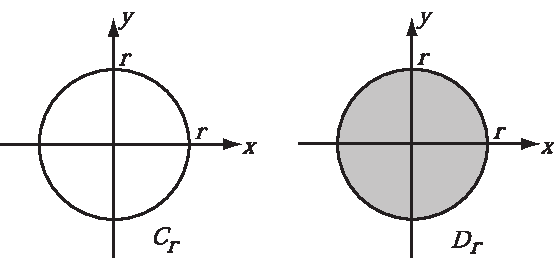
\includegraphics[width=\linewidth]{external/figps-activitycircles.pdf}
\end{image}%
\tcblower
\end{figureptx}%
%
\begin{enumerate}[font=\bfseries,label=(\alph*),ref=\alph*]
\item{}Determine \(\bigcup\limits_{r \in \R^*}^{}C_r\) and \(\bigcap\limits_{r \in \R^*}^{}C_r\).%
\item{}Determine \(\bigcup\limits_{r \in \R^*}^{}D_r\) and \(\bigcap\limits_{r \in \R^*}^{}D_r\).%
\item{}Determine \(\bigcup\limits_{r \in \R^*}^{}T_r\) and \(\bigcap\limits_{r \in \R^*}^{}T_r\).%
\item{}Let \(\mathscr{C} = \left\{ C_r \mid r \in \R^* \right\}\), \(\mathscr{D} = \left\{ D_r \mid r \in \R^* \right\}\), and \(\mathscr{T} = \left\{ T_r \mid r \in \R^* \right\}\). Are any of these indexed families of sets pairwise disjoint? Explain.%
\par
Now let \(I\) be the closed interval \([0, 2]\) and let \(J\) be the closed interval \([1, 2]\).%
\item{}Determine \(\bigcup\limits_{r \in I}^{}C_r\), \(\bigcap\limits_{r \in I}^{}C_r\), \(\bigcup\limits_{r \in J}^{}C_r\), and \(\bigcap\limits_{r \in J}^{}C_r\).%
\item{}Determine \(\bigcup\limits_{r \in I}^{}D_r\), \(\bigcap\limits_{r \in I}^{}D_r\), \(\bigcup\limits_{r \in J}^{}D_r\), and \(\bigcap\limits_{r \in J}^{}D_r\).%
\item\label{x:task:A_indexfamily7}Determine \(\left(\: \bigcup\limits_{r \in I}^{}D_r \right)^c\), \(\left(\: \bigcap\limits_{r \in I}^{}D_r \right)^c\), \(\left(\: \bigcup\limits_{r \in J}^{}D_r \right)^c\), and \(\left(\: \bigcap\limits_{r \in J}^{}D_r \right)^c\).%
\item\label{x:task:A_indexfamily8}Determine \(\bigcup\limits_{r \in I}^{}T_r\), \(\bigcap\limits_{r \in I}^{}T_r\), \(\bigcup\limits_{r \in J}^{}T_r\), and \(\bigcap\limits_{r \in J}^{}T_r\).%
\item{}Use De Morgan's Laws to explain the relationship between your answers in \hyperref[x:task:A_indexfamily7]{Task~{\xreffont\ref{x:activity:A_indexfamiliy}}.{\xreffont\ref{x:task:A_indexfamily7}}, p.\,\pageref{x:task:A_indexfamily7}} and \hyperref[x:task:A_indexfamily8]{Task~{\xreffont\ref{x:activity:A_indexfamiliy}}.{\xreffont\ref{x:task:A_indexfamily8}}, p.\,\pageref{x:task:A_indexfamily8}}.%
\end{enumerate}
\end{activity}%
\end{exercises-subsection}
\end{sectionptx}
%
%
\typeout{************************************************}
\typeout{Section 5.6 Chapter~{\xreffont\ref*{x:chapter:C_settheory}} Summary}
\typeout{************************************************}
%
\begin{sectionptx}{Chapter~{\xreffont\ref*{x:chapter:C_settheory}} Summary}{}{Chapter~{\xreffont\ref*{x:chapter:C_settheory}} Summary}{}{}{x:section:S_5summary}
%
%
\typeout{************************************************}
\typeout{Subsection  Important Definitions}
\typeout{************************************************}
%
\begin{subsectionptx}{Important Definitions}{}{Important Definitions}{}{}{g:subsection:idm822004504}
%
\begin{itemize}[label=\textbullet]
\item{}\hyperref[x:assemblage:D_setequality]{Equal Sets, p.\,\pageref{x:assemblage:D_setequality}}%
\item{}\hyperref[x:assemblage:D_setequality]{Subset, p.\,\pageref{x:assemblage:D_setequality}}%
\item{}\hyperref[x:assemblage:propersubset]{Proper subset, p.\,\pageref{x:assemblage:propersubset}}%
\item{}\hyperref[x:assemblage:D_powerset]{Power set, p.\,\pageref{x:assemblage:D_powerset}}%
\item{}\hyperref[x:assemblage:D_cardinality]{Cardinality of a finite set, p.\,\pageref{x:assemblage:D_cardinality}}%
\item{}\hyperref[x:assemblage:intersection]{Intersection of two sets, p.\,\pageref{x:assemblage:intersection}}%
\item{}\hyperref[x:assemblage:intersection]{Union of two sets, p.\,\pageref{x:assemblage:intersection}}%
\item{}\hyperref[x:assemblage:setdiff]{Set difference, p.\,\pageref{x:assemblage:setdiff}}%
\item{}\hyperref[x:assemblage:setdiff]{Complement of a set, p.\,\pageref{x:assemblage:setdiff}}%
\item{}\hyperref[x:assemblage:D_disjointsets]{Disjoint sets, p.\,\pageref{x:assemblage:D_disjointsets}}%
\item{}\hyperref[x:assemblage:cartesianproduct]{Cartesian product of two sets, p.\,\pageref{x:assemblage:cartesianproduct}}%
\item{}\hyperref[x:assemblage:orderedpair]{Ordered pair, p.\,\pageref{x:assemblage:orderedpair}}%
\item{}\hyperref[x:assemblage:D_familyoper]{Union over a family of sets, p.\,\pageref{x:assemblage:D_familyoper}}%
\item{}\hyperref[x:assemblage:D_familyoper]{Intersection over a family of sets, p.\,\pageref{x:assemblage:D_familyoper}}%
\item{}\hyperref[x:assemblage:D_indexfamily]{Indexing set, p.\,\pageref{x:assemblage:D_indexfamily}}%
\item{}\hyperref[x:assemblage:D_indexfamily]{Indexed family of sets, p.\,\pageref{x:assemblage:D_indexfamily}}%
\item{}\hyperref[x:assemblage:D_indexoper]{Union over an indexed family of sets, p.\,\pageref{x:assemblage:D_indexoper}}%
\item{}\hyperref[x:assemblage:D_indexoper]{Intersection over an indexed family of sets, p.\,\pageref{x:assemblage:D_indexoper}}%
\item{}\hyperref[x:assemblage:D_disjointfamily]{Pairwise disjoint family of sets, p.\,\pageref{x:assemblage:D_disjointfamily}}%
\end{itemize}
\end{subsectionptx}
%
%
\typeout{************************************************}
\typeout{Subsection  Important Theorems and Results about Sets}
\typeout{************************************************}
%
\begin{subsectionptx}{Important Theorems and Results about Sets}{}{Important Theorems and Results about Sets}{}{}{g:subsection:idm821979160}
%
\begin{itemize}[label=\textbullet]
\item{}\hyperref[x:theorem:T_powerset]{Theorem~{\xreffont\ref{x:theorem:T_powerset}}, p.\,\pageref{x:theorem:T_powerset}}%
\item{}\hyperref[x:theorem:T_algebraofsets]{Theorem~{\xreffont\ref{x:theorem:T_algebraofsets}}, p.\,\pageref{x:theorem:T_algebraofsets}}%
\item{}\hyperref[x:theorem:T_propsofcomplements]{Theorem~{\xreffont\ref{x:theorem:T_propsofcomplements}}, p.\,\pageref{x:theorem:T_propsofcomplements}}%
\item{}\hyperref[x:theorem:T_propsofcartprod]{Theorem~{\xreffont\ref{x:theorem:T_propsofcartprod}}, p.\,\pageref{x:theorem:T_propsofcartprod}}%
\item{}\hyperref[x:theorem:T_indexproperties]{Theorem~{\xreffont\ref{x:theorem:T_indexproperties}}, p.\,\pageref{x:theorem:T_indexproperties}}%
\item{}\hyperref[x:theorem:T_distributeindex]{Theorem~{\xreffont\ref{x:theorem:T_distributeindex}}, p.\,\pageref{x:theorem:T_distributeindex}}%
\end{itemize}
\end{subsectionptx}
%
%
\typeout{************************************************}
\typeout{Subsection  Important Proof Method}
\typeout{************************************************}
%
\begin{subsectionptx}{Important Proof Method}{}{Important Proof Method}{}{}{g:subsection:idm821973528}
%
%
\typeout{************************************************}
\typeout{Subsubsection  The Choose-an-Element Method}
\typeout{************************************************}
%
\begin{subsubsectionptx}{The Choose-an-Element Method}{}{The Choose-an-Element Method}{}{}{g:subsubsection:idm821977240}
The choose-an-element method is frequently used when we encounter a universal quantifier in a statement in the backward process of a proof. This statement often has the form \begin{quote}%
For each elemet with a given property, something happens.\end{quote}
  In the forward process of the proof, we then choose an arbitrary element with the given property. \begin{quote}%
\emph{Whenever we choose an arbitrary element with a given property, we are not selecting a specific element. Rather, the only thing we can assume about the element is the given property.}\end{quote}
 For more information, see \hyperref[x:subsection:SS_choosemethod]{The Choose-an-Element Method, p.\,\pageref{x:subsection:SS_choosemethod}}.%
\end{subsubsectionptx}
\end{subsectionptx}
\end{sectionptx}
\end{chapterptx}
%
%
\typeout{************************************************}
\typeout{Chapter 6 Functions}
\typeout{************************************************}
%
\begin{chapterptx}{Functions}{}{Functions}{}{}{x:chapter:C_functions}
%
%
\typeout{************************************************}
\typeout{Section 6.1 Introduction to Functions}
\typeout{************************************************}
%
\begin{sectionptx}{Introduction to Functions}{}{Introduction to Functions}{}{}{x:section:S_introfunctions}
%
%
\typeout{************************************************}
\typeout{Beginning Activity  Beginning Activity 1: Functions from Previous Courses}
\typeout{************************************************}
%
\begin{worksheet-subsection}{Beginning Activity 1: Functions from Previous Courses}{}{Beginning Activity 1: Functions from Previous Courses}{}{}{x:worksheet:PA_previousfunctions}
\index{function}%
\index{domain!of a function}%
\index{function!domain}%
\index{codomain}%
\index{function!codomain}%
One of the most important concepts in modern mathematics is that of a \terminology{function}. In previous mathematics courses, we have often thought of a function as some sort of input-output rule that assigns exactly one output to each input. So in this context, a \terminology{function} can be thought of as a procedure for associating with each element of some set, called the \terminology{domain of the function}, exactly one element of another set, called the \terminology{codomain of the function}. This procedure can be considered an input-output rule. The function takes the input, which is an element of the domain, and produces an output, which is an element of the codomain. In calculus and precalculus, the inputs and outputs were almost always real numbers. So the notation \(f( x ) = x^2 \sin x\) means the following:%
\begin{itemize}[label=\textbullet]
\item{}\(f\) is the name of the function.%
\item{}\(f( x )\) is a real number. It is the output of the function when the input is the real number  \(x\). For example,%
\begin{align*}
f\left( {\frac{\pi }{2}} \right) \amp = \left( {\frac{\pi }{2}} \right)^2 
\sin \left( {\frac{\pi } {2}} \right)\\
\amp = \frac{{\pi ^2 }}{4} \cdot 1\\
\amp = \frac{{\pi ^2 }}{4}\text{.}
\end{align*}
%
\end{itemize}
For this function, it is understood that the domain of the function is the set \(\R\) of all real numbers. In this situation, we think of the domain as the set of all possible inputs. That is, the domain is the set of all possible real numbers \(x\) for which a real number output can be determined.%
\par
This is closely related to the equation \(y = x^2 \sin x\). With this equation, we frequently think of \(x\) as the input and \(y\) as the output. In fact, we sometimes write \(y = f( x )\). The key to remember is that a function must have exactly one output for each input. When we write an equation such as%
\begin{equation*}
y = \dfrac{1}{2}x^3  - 1\text{,}
\end{equation*}
we can use this equation to define \(y\) as a function of \(x\). This is because when we substitute a real number for \(x\) (the input), the equation produces exactly one real number for \(y\) (the output). We can give this function a name, such as \(g\), and write%
\begin{equation*}
y = g( x ) = \frac{1}{2}x^3  - 1\text{.}
\end{equation*}
However, as written, an equation such as%
\begin{equation*}
y^2  = x + 3
\end{equation*}
cannot be used to define \(y\) as a function of \(x\) since there are real numbers that can be substituted for \(x\) that will produce more than one possible value of \(y\). For example, if \(x = 1\), then \(y^2  = 4\), and \(y\) could be \(-2\) or 2.%
\par
Which of the following equations can be used to define a function with \(x \in \R\) as the input and \(y \in \R\) as the output?%
\begin{divisionexercise}{1}{}{}{g:exercise:idm821949720}%
\(y = x^2 - 2\)%
\end{divisionexercise}%
\begin{divisionexercise}{2}{}{}{g:exercise:idm821948568}%
\(y^2 = x + 3\)%
\end{divisionexercise}%
\begin{divisionexercise}{3}{}{}{g:exercise:idm821943960}%
\(y = \dfrac{1}{2}x^3 - 1\)%
\end{divisionexercise}%
\begin{divisionexercise}{4}{}{}{g:exercise:idm821943832}%
\(y = \dfrac{1}{2} x\sin x\)%
\end{divisionexercise}%
\begin{divisionexercise}{5}{}{}{g:exercise:idm821938840}%
\(x^2 + y^2 = 4\)%
\end{divisionexercise}%
\begin{divisionexercise}{6}{}{}{g:exercise:idm821943576}%
\(y = 2x - 1\)%
\end{divisionexercise}%
\begin{divisionexercise}{7}{}{}{g:exercise:idm821943320}%
\(y = \dfrac{x}{{x - 1}}\)%
\end{divisionexercise}%
\end{worksheet-subsection}
%
%
\typeout{************************************************}
\typeout{Beginning Activity  Beginning Activity 2: Some Other Types of Functions}
\typeout{************************************************}
%
\begin{worksheet-subsection}{Beginning Activity 2: Some Other Types of Functions}{}{Beginning Activity 2: Some Other Types of Functions}{}{}{x:worksheet:PA_otherfunctions}
The domain and codomain of each of the functions in \hyperref[x:worksheet:PA_previousfunctions]{Beginning Activity 1, p.\,\pageref{x:worksheet:PA_previousfunctions}} are the set \(\R\) of all real numbers, or some subset of \(\R\). In most of these cases, the way in which the function associates elements of the domain with elements of the codomain is by a rule determined by some mathematical expression. For example, when we say that \(f\) is the function such that%
\begin{equation*}
f( x ) = \dfrac{x}{{x - 1}}\text{,}
\end{equation*}
then the algebraic rule that determines the output of the function \(f\) when the input is \(x\) is \(\dfrac{x}{{x - 1}}\). In this case, we would say that the domain of \(f\) is the set of all real numbers not equal to 1 since division by zero is not defined.%
\par
However, the concept of a function is much more general than this. The domain and codomain of a function can be any set, and the way in which a function associates elements of the domain with elements of the codomain can have many different forms. The input-output rule for a function can be a formula, a graph, a table, a random process, or a verbal description. We will explore two different examples in this activity.%
\begin{divisionexercise}{1}{}{}{g:exercise:idm821935896}%
Let \(b\) be the function that assigns to each person his or her birthday (month and day). The domain of the function \(b\) is the set of all people and the codomain of \(b\) is the set of all days in a leap year (i.e., January 1 through December 31, including February 29).%
\begin{enumerate}[font=\bfseries,label=(\alph*),ref=\alph*]
\item{}\index{birthday function}%
Explain why \(b\) really is a function. We will call this the \terminology{birthday function}.%
\item{}\index{Wiles, Andrew}%
In 1995, Andrew Wiles became famous for publishing a proof of Fermat's Last Theorem. (See A. D. Aczel, \pubtitle{Fermat's Last Theorem: Unlocking the Secret of an Ancient Mathematical Problem}, Dell Publishing, New York, 1996.) Andrew Wiles's birthday is April 11, 1953. Translate this fact into functional notation using the ``birthday function'' \(b\). That is, fill in the spaces for the following question marks:%
\begin{equation*}
b( {\,?\,} ) = \,?\text{.}
\end{equation*}
%
\item{}Is the following statement true or false? Explain.%
\begin{quote}%
For each day \(D\) of the year, there exists a person \(x\) such that \(b( x ) = D\).\end{quote}
\item{}Is the following statement true or false? Explain.%
\begin{quote}%
For any people \(x\) and \(y\), if \(x\) and \(y\) are different people, then \(b( x ) \ne b( y )\).\end{quote}
\end{enumerate}
\end{divisionexercise}%
\begin{divisionexercise}{2}{}{}{x:exercise:sym_sumdivisors}%
\index{sum of divisors function}%
\label{g:notation:idm821928728} Let  \(s\) be the function that associates with each natural number the sum of its distinct natural number divisors. This is called the \terminology{sum of the divisors function}. For example, the natural number divisors of 6 are 1, 2, 3, and 6, and so%
\begin{align*}
s( 6 ) \amp = 1 + 2 + 3 + 6\\
\amp = 12\text{.}
\end{align*}
%
\begin{enumerate}[font=\bfseries,label=(\alph*),ref=\alph*]
\item{}Calculate \(s( k )\) for each natural number \(k\) from 1 through 15.%
\item\label{x:task:sym_sumdivisorsb}Does there exist a natural number \(n\) such that \(s( n ) = 5\)? Justify your conclusion.%
\item\label{x:task:sym_sumdivisorsc}Is it possible to find two different natural numbers \(m\) and \(n\) such that \(s( m ) = s( n )\)? Explain.%
\item{}Use your responses in \hyperref[x:task:sym_sumdivisorsb]{Task~{\xreffont 2}.{\xreffont\ref{x:task:sym_sumdivisorsb}}, p.\,\pageref{x:task:sym_sumdivisorsb}} \hyperref[x:task:sym_sumdivisorsc]{Task~{\xreffont 2}.{\xreffont\ref{x:task:sym_sumdivisorsc}}, p.\,\pageref{x:task:sym_sumdivisorsc}} to determine the truth value of each of the following statements.%
\begin{enumerate}[font=\bfseries,label=(\roman*),ref=\theenumi.\roman*]
\item{}For each \(m \in \mathbb{N}\), there exists a natural number \(n\) such that \(s( n ) = m\).%
\item{}For all \(m, n \in \mathbb{N}\), if \(m \ne n\), then \(s( m ) \ne s( n )\).%
\end{enumerate}
\end{enumerate}
\end{divisionexercise}%
\end{worksheet-subsection}
%
%
\typeout{************************************************}
\typeout{Subsection  The Definition of a Function}
\typeout{************************************************}
%
\begin{subsectionptx}{The Definition of a Function}{}{The Definition of a Function}{}{}{g:subsection:idm821913752}
The concept of a function is much more general than the idea of a function used in calculus or precalculus. In particular, the domain and codomain do not have to be subsets of \(\mathbb{R}\). In addition, the way in which a function associates elements of the domain with elements of the codomain can have many different forms. This input-output rule can be a formula, a graph, a table, a random process, a computer algorithm, or a verbal description. Two such examples were introduced in \hyperref[x:worksheet:PA_otherfunctions]{Beginning Activity 2, p.\,\pageref{x:worksheet:PA_otherfunctions}}.%
\par
\index{birthday function}\index{sum of divisors function} For the \terminology{birthday function}, the domain would be the set of all people and the codomain would be the set of all days in a leap year. For the \terminology{sum of the divisors function}, the domain is the set \(\mathbb{N}\) of natural numbers, and the codomain could also be \(\mathbb{N}\). In both of these cases, the input-output rule was a verbal description of how to assign an element of the codomain to an element of the domain.%
\par
We formally define the concept of a function as follows:%
\begin{assemblage}{Definition.}{x:assemblage:function}%
A \terminology{function} from a set \(A\) to a set \(B\) is a rule that associates with each element \(x\) of the set \(A\) exactly one element of the set \(B\). A function from \(A\) to \(B\) is also called a \terminology{mapping} from \(A\) to \(B\).%
\end{assemblage}
\begin{paragraphs}{Function Notation.}{x:paragraphs:sym_function}%
\label{g:notation:idm821899160}%
When we work with a function, we usually give it a name. The name is often a single letter, such as \(f\) or \(g\). If \(f\) is a function from the set \(A\) to the set \(B\), we will write \(f \colon A \to B\). This is simply shorthand notation for the fact that \(f\) is a function from the set \(A\) to the set \(B\). In this case, we also say that \(f\) maps \(A\) to \(B\).%
\end{paragraphs}%
\begin{assemblage}{Definition.}{x:assemblage:domainfunction}%
\label{g:notation:idm821890712}\label{g:notation:idm821893784}\label{g:notation:idm821891736} Let \(f \colon A \to B\). (This is read, ``Let \(f\) be a function from \(A\) to \(B\).'' ) The set \(A\) is called the \terminology{domain} of the function \(f\), and we write \(A = \text{ dom} ( f )\). The set \(B\) is called the \terminology{codomain} of the function \(f\), and we write \(B = \text{ codom} ( f )\). If \(a \in A\), then the element of \(B\) that is associated with \(a\) is denoted by \(f( a )\) and is called the \terminology{image of \(\boldsymbol{a}\) under \(\boldsymbol{f}\)}. If \(f( a ) = b\), with \(b \in B\), then \(a\) is called a \terminology{preimage of \(\boldsymbol{b}\) for \(\boldsymbol{f}\)}.%
\end{assemblage}
\begin{paragraphs}{Some Function Terminology with an Example.}{x:paragraphs:functionterms}%
. \index{independent variable}%
\index{variable!independent}%
\index{dependent variable}%
\index{variable!dependent}%
When we have a function \(f \colon A \to B\), we often write \(y = f(x)\). In this case, we consider \(x\) to be an unspecified object that can be chosen from the set \(A\), and we would say that \(x\) is the \terminology{independent variable} of the function \(f\) and \(y\) is the \terminology{dependent variable} of the function \(f\).%
\par
For a specific example, consider the function \(g \x \mathbb{R} \to \mathbb{R}\), where \(g( x )\) is defined by the formula%
\begin{equation*}
g( x ) = x^2  - 2\text{.}
\end{equation*}
Note that this is indeed a function since given any input \(x\) in the domain, \(\R\), there is exactly one output \(g( x )\) in the codomain, \(\R\). For example,%
\begin{align*}
g( { - 2} ) \amp = \left( { - 2} \right)^2  - 2 = 2,\\
g( 5 ) \amp = 5^2  - 2 = 23,\\
g( {\sqrt 2 } ) \amp = \left( {\sqrt 2 } \right)^2  - 2 = 0,\\
g( { - \sqrt 2 } ) \amp = \left( { - \sqrt 2 } \right)^2  - 2 = 0\text{.}
\end{align*}
So we say that the image of \(-2\) under \(g\) is 2, the image of 5 under \(g\) is 23, and so on.%
\par
Notice in this case that the number 0 in the codomain has two preimages, \(- \sqrt 2 \text{ and } \sqrt 2\). This does not violate the mathematical definition of a function since the definition only states that each input must produce one and only one output. That is, each element of the domain has exactly one image in the codomain. Nowhere does the definition stipulate that two different inputs must produce different outputs.%
\par
Finding the preimages of an element in the codomain can sometimes be difficult. In general, if \(y\) is in the codomain, to find its preimages, we need to ask, ``For which values of \(x\) in the domain will we have \(y = g( x )\)?'' For example, for the function \(g\), to find the preimages of 5, we need to find all \(x\) for which \(g( x ) = 5\). In this case, since \(g( x ) = x^2  - 2\), we can do this by solving the equation%
\begin{equation*}
x^2  - 2 = 5\text{.}
\end{equation*}
The solutions of this equation are \(- \sqrt 7\) and \(\sqrt 7\). So for the function \(g\), the preimages of 5 are \(- \sqrt 7\) and \(\sqrt 7\). We often use set notation for this and say that the set of preimages of 5 for the function \(g\) is \(\left\{ -\sqrt{7}, \sqrt{7} \right\}\).%
\par
Also notice that for this function, not every element in the codomain has a preimage. For example, there is no input \(x\) such that \(g\left( x \right) = - 3\). This is true since for all real numbers \(x\), \(x^2 \geq 0\) and hence \(x^2 - 2 \geq - 2\). This means that for all \(x\) in \(\mathbb{R}\), \(g\left( x \right) \geq - 2\).%
\par
Finally, note that we introduced the function \(g\) with the sentence, ``Consider the function \(g\x \mathbb{R} \to \mathbb{R}\), where \(g( x )\) is defined by the formula \(g( x ) = x^2 - 2\).'' This is one correct way to do this, but we will frequently shorten this to, ``Let \(g\x \mathbb{R} \to \mathbb{R}\) be defined by \(g( x ) = x^2 - 2\)'', or ``Let \(g\x \mathbb{R} \to \mathbb{R}\), where \(g( x ) = x^2 - 2\).''%
\end{paragraphs}%
\begin{inlineexercise}{Images and Preimages.}{x:exercise:pr_images}%
Let \(f\x \R \to \R\) be defined by \(f(x) = x^2 - 5x\) for all \(x \in \R\), and let \(g\x \Z \to \Z\) be defined by \(g(m) = m^2 - 5m\) for all \(m \in \Z\).%
\begin{enumerate}[font=\bfseries,label=(\alph*),ref=\alph*]
\item{}Determine \(f ( -3 )\) and \(f \left( \sqrt 8 \right)\).%
\space\hyperlink{g:solution:idm821706776-back}{[Solution]}\item{}Determine \(g ( 2 )\) and \(g ( -2 )\).%
\space\hyperlink{g:solution:idm821703576-back}{[Solution]}\item{}Determine the set of all preimages of 6 for the function \(f\).%
\space\hyperlink{g:solution:idm821693720-back}{[Solution]}\item{}Determine the set of all preimages of 6 for the function \(g\).%
\space\hyperlink{g:solution:idm821698328-back}{[Solution]}\item{}Determine the set of all preimages of 2 for the function \(f\).%
\space\hyperlink{g:solution:idm821696536-back}{[Solution]}\item{}Determine the set of all preimages of 2 for the function \(g\).%
\space\hyperlink{g:solution:idm821696152-back}{[Solution]}\end{enumerate}
\end{inlineexercise}%
\end{subsectionptx}
%
%
\typeout{************************************************}
\typeout{Subsection  The Codomain and Range of a Function}
\typeout{************************************************}
%
\begin{subsectionptx}{The Codomain and Range of a Function}{}{The Codomain and Range of a Function}{}{}{g:subsection:idm821695640}
Besides the domain and codomain, there is another important set associated with a function. The need for this was illustrated in the example of the function \(g\) in \hyperlink{x:paragraphs:functionterms}{Some Function Terminology with an Example, p.\,\pageref{x:paragraphs:functionterms}}. For this function, it was noticed that there are elements in the codomain that have no preimage or, equivalently, there are elements in the codomain that are not the image of any element in the domain. The set we are talking about is the subset of the codomain consisting of all images of the elements of the domain of the function, and it is called the range of the function.%
\begin{assemblage}{Definition.}{x:assemblage:rangeandimage}%
\label{g:notation:idm821689880} Let \(f\x A \to B\). The set \(\left\{ {f( x ) \mid x \in A} \right\}\) is called the \terminology{range of the function \(\boldsymbol{f}\)} and is denoted by \(\text{ range} \left( f \right)\). The range of \(f\) is sometimes called the \terminology{image of the function \(\boldsymbol{f}\)} (or the \terminology{image of \(\boldsymbol{A}\) under \(\boldsymbol{f}\)}).%
\end{assemblage}
The range of \(f\x A \to B\) could equivalently be defined as follows:%
\begin{equation*}
\text{ range} ( f ) = \left\{ { {y \in B} \mid y = f\left( x \right)\text{ for some } x 
\in A} \right\}\!\text{.}
\end{equation*}
Notice that this means that \(\text{ range} (f) \subseteq \text{ codom} (f)\) but does not necessarily mean that \(\text{ range} (f) = \text{ codom} (f)\). Whether we have this set equality or not depends on the function \(f\). More about this will be explored in \hyperref[x:section:S_typesoffunctions]{Section~{\xreffont\ref{x:section:S_typesoffunctions}}, p.\,\pageref{x:section:S_typesoffunctions}}.%
\begin{inlineexercise}{Codomain and Range.}{x:exercise:pr_codomainandrange1}%
\begin{enumerate}[font=\bfseries,label=(\alph*),ref=\alph*]
\item{}Let \(b\) be the function that assigns to each person his or her birthday (month and day).%
\begin{enumerate}[font=\bfseries,label=(\roman*),ref=\theenumi.\roman*]
\item{}What is the domain of this function?%
\space\hyperlink{g:solution:idm821681816-back}{[Solution]}\item{}What is a codomain for this function?%
\space\hyperlink{g:solution:idm821676696-back}{[Solution]}\item{}In \hyperref[x:worksheet:PA_otherfunctions]{Beginning Activity 2, p.\,\pageref{x:worksheet:PA_otherfunctions}}, we determined that the following statement is true: For each day \(D\) of the year, there exists a person \(x\) such that \(b( x ) = D\). What does this tell us about the range of the function \(b\)? Explain.%
\space\hyperlink{g:solution:idm821674648-back}{[Solution]}\end{enumerate}
\item{}Let \(s\) be the function that associates with each natural number the sum of its distinct natural number factors.%
\begin{enumerate}[font=\bfseries,label=(\roman*),ref=\theenumi.\roman*]
\item{}What is the domain of this function?%
\space\hyperlink{g:solution:idm821671576-back}{[Solution]}\item{}What is a codomain for this function?%
\space\hyperlink{g:solution:idm821670936-back}{[Solution]}\item{}In \hyperref[x:worksheet:PA_otherfunctions]{Beginning Activity 2, p.\,\pageref{x:worksheet:PA_otherfunctions}}, we determined that the following statement is false: \begin{quote}%
For each \(m \in \mathbb{N}\), there exists a natural number \(n\) such that \(s( n ) = m\).\end{quote}
 Give an example of a natural number \(m\) that shows this statement is false, and explain what this tells us about the range of the function \(s\).%
\space\hyperlink{g:solution:idm821659928-back}{[Solution]}\end{enumerate}
\end{enumerate}
\end{inlineexercise}%
\end{subsectionptx}
%
%
\typeout{************************************************}
\typeout{Subsection  The Graph of a Real Function}
\typeout{************************************************}
%
\begin{subsectionptx}{The Graph of a Real Function}{}{The Graph of a Real Function}{}{}{x:subsection:realfunction}
We will finish this section with methods to visually communicate information about two specific types of functions. The first is the familiar method of graphing functions that was a major part of some previous mathematics courses. For example, consider the function \(g \x \R \to \R\) defined by \(g(x) = x^2 - 2x - 1\).%
\begin{figureptx}{Graph of \(y = g( x )\), where  \(g( x ) = x^2  - 2x - 1\)}{x:figure:fig_functiongraph1}{}%
\begin{image}{0.275}{0.45}{0.275}%
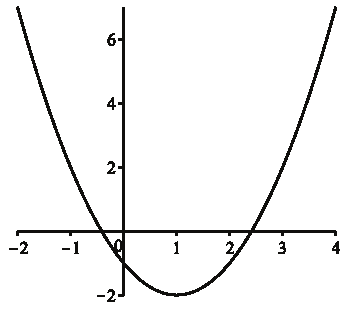
\includegraphics[width=\linewidth]{external/figps-graphsec6-1.pdf}
\end{image}%
\tcblower
\end{figureptx}%
\index{real function}\index{function!real} Every point on this graph corresponds to an ordered pair \(\left( {x,\;y} \right)\) of real numbers, where \(y = g( x ) = x^2  - 2x - 1\). Because we use the Cartesian plane when drawing this type of graph, we can only use this type of graph when both the domain and the codomain of the function are subsets of the real numbers \(\R\). Such a function is sometimes called a \terminology{real function}. The graph of a real function is a visual way to communicate information about the function. For example, the range of \(g\) is the set of all \(y\)-values that correspond to points on the graph. In this case, the graph of \(g\) is a parabola and has a vertex at the point \((1, -2)\). (Note: The \(x\)-coordinate of the vertex can be found by using calculus and solving the equation \(f ' (x) = 0\).) Since the graph of the function \(g\) is a parabola, we know that the pattern shown on the left end and the right end of the graph continues and we can conclude that the range of \(g\) is the set of all \(y \in \R\) such that \(y \geq -2\). That is,%
\begin{equation*}
\text{ range}  (g) = \{ y \in \R \mid y \geq -2 \}\text{.}
\end{equation*}
%
\begin{inlineexercise}{Using the Graph of a Real Function.}{x:exercise:pr_graphreal}%
The graph in \hyperref[x:figure:fig_functiongraph2]{Figure~{\xreffont\ref{x:figure:fig_functiongraph2}}, p.\,\pageref{x:figure:fig_functiongraph2}} shows the graph of (slightly more than) two complete periods for a function \(f \x \R \to \R\), where \(f(x) = A \sin (Bx)\) for some positive real number constants \(A\) and \(B\).%
\begin{figureptx}{Graph of \(y = f( x )\)}{x:figure:fig_functiongraph2}{}%
\begin{image}{0.275}{0.45}{0.275}%
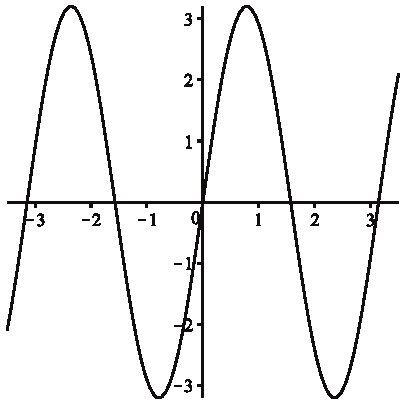
\includegraphics[width=\linewidth]{external/figps-graph2sec6-1.pdf}
\end{image}%
\tcblower
\end{figureptx}%
\begin{enumerate}[font=\bfseries,label=(\alph*),ref=\alph*]
\item{}We can use the graph to estimate the output for various inputs. This is done by estimating the \(y\)-coordinate for the point on the graph with a specified \(x\)-coordinate. On the graph, draw vertical lines at \(x = - 1\) and \(x = 2\) and estimate the values of \(f( { - 1} )\) and \(f( 2 )\).%
\space\hyperlink{g:solution:idm821643032-back}{[Solution]}\item{}Similarly, we can estimate inputs of the function that produce a specified output. This is done by estimating the \(x\)-coordinates of the points on the graph that have a specified \(y\)-coordinate. Draw a horizontal line at \(y = 2\) and estimate at least two values of \(x\) such that \(f( x ) = 2\).%
\space\hyperlink{g:solution:idm821646360-back}{[Solution]}\item{}Use the graph in \hyperref[x:figure:fig_functiongraph2]{Figure~{\xreffont\ref{x:figure:fig_functiongraph2}}, p.\,\pageref{x:figure:fig_functiongraph2}} to estimate the range of the function \(f\).%
\space\hyperlink{g:solution:idm821637144-back}{[Solution]}\end{enumerate}
\end{inlineexercise}%
\end{subsectionptx}
%
%
\typeout{************************************************}
\typeout{Subsection  Arrow Diagrams}
\typeout{************************************************}
%
\begin{subsectionptx}{Arrow Diagrams}{}{Arrow Diagrams}{}{}{g:subsection:idm821635352}
\index{arrow diagram}%
Sometimes the domain and codomain of a function are small, finite sets. When this is the case, we can define a function simply by specifying the outputs for each input in the domain. For example, if we let \(A = \left\{ {1, 2, 3} \right\}\) and let \(B = \left\{ {a, b} \right\}\), we can define a function \(F\x A \to B\) by specifying that%
\begin{equation*}
F( 1 ) = a, F( 2 ) = a, \text{ and }   F( 3 ) = b\text{.}
\end{equation*}
This is a function since each element of the domain is mapped to exactly one element in \(B\). A convenient way to illustrate or visualize this type of function is with a so-called \terminology{arrow diagram} as shown in \hyperref[x:figure:fig_arrow61-1]{Figure~{\xreffont\ref{x:figure:fig_arrow61-1}}, p.\,\pageref{x:figure:fig_arrow61-1}}.%
\begin{figureptx}{Arrow Diagram for a Function}{x:figure:fig_arrow61-1}{}%
\begin{image}{0.35}{0.3}{0.35}%
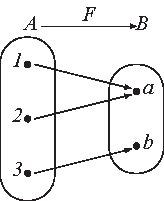
\includegraphics[width=\linewidth]{external/figps-arrow61-1x.pdf}
\end{image}%
\tcblower
\end{figureptx}%
An arrow diagram can be used when the domain and codomain of the function are finite (and small). We represent the elements of each set with points and then use arrows to show how the elements of the domain are associated with elements of the codomain. For example, the arrow from the point 2 in \(A\) to the point \(a\) in \(B\) represents the fact that \(F( 2 ) = a\). In this case, we can use the arrow diagram in \hyperref[x:figure:fig_arrow61-1]{Figure~{\xreffont\ref{x:figure:fig_arrow61-1}}, p.\,\pageref{x:figure:fig_arrow61-1}} to conclude that \(\text{ range} (F) = \{ a, b \}\).%
\begin{inlineexercise}{Working with Arrow Diagrams.}{x:exercise:pr_arrow}%
Let \(A = \left\{ {1, 2, 3, 4} \right\}\) and let \(B = \left\{ {a, b, c} \right\}\).%
\begin{figureptx}{Arrow Diagrams}{x:figure:fig_arrow61-2}{}%
\begin{image}{0.1}{0.8}{0.1}%
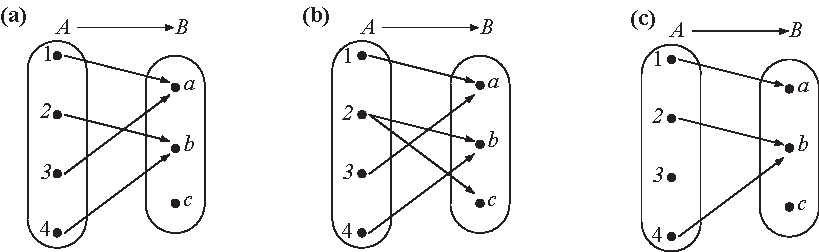
\includegraphics[width=\linewidth]{external/figps-arrow-exer611abc.pdf}
\end{image}%
\tcblower
\end{figureptx}%
\begin{enumerate}[font=\bfseries,label=(\alph*),ref=\alph*]
\item\label{x:task:exer_sec61-1}Which of the arrow diagrams in \hyperref[x:figure:fig_arrow61-2]{Figure~{\xreffont\ref{x:figure:fig_arrow61-2}}, p.\,\pageref{x:figure:fig_arrow61-2}} can be used to represent a function from \(A\) to \(B\)? Explain.%
\item{}For those arrow diagrams that can be used to represent a function from \(A\) to \(B\), determine the range of the function.%
\space\hyperlink{g:solution:idm821634712-back}{[Solution]}\end{enumerate}
\end{inlineexercise}%
\end{subsectionptx}
%
%
\typeout{************************************************}
\typeout{Exercises  Exercises}
\typeout{************************************************}
%
\begin{exercises-subsection}{Exercises}{}{Exercises}{}{}{g:exercises:idm821625240}
\begin{divisionexercise}{1}{}{}{g:exercise:idm821623576}%
Let \(f\x \mathbb{R} \to \mathbb{R}\) be defined by \(f\left( x \right) = x^2 - 2x\).%
\begin{enumerate}[font=\bfseries,label=(\alph*),ref=\alph*]
\item{}Evaluate \(f( { - 3} ), f( { - 1} ), f( 1 ), \text{ and } f( 3 )\).%
\space\hyperlink{g:answer:idm821621400-back}{[Answer]}\item{}Determine the set of all of the preimages of 0 and the set of all of the preimages of 4.%
\space\hyperlink{g:answer:idm821623832-back}{[Answer]}\item{}Sketch a graph of the function \(f\).%
\item{}Determine the range of the function \(f\).%
\space\hyperlink{g:answer:idm821613208-back}{[Answer]}\end{enumerate}
\end{divisionexercise}%
\begin{divisionexercise}{2}{}{}{g:exercise:idm821610648}%
Let \(\mathbb{R}^* = \left\{ { {x \in \mathbb{R}} \mid x \geq 0} \right\}\), and let \(s\x \mathbb{R} \to \mathbb{R}^*\) be defined by \(s( x ) = x^2\).%
\begin{enumerate}[font=\bfseries,label=(\alph*),ref=\alph*]
\item{}Evaluate \(s( { - 3} ), s( { - 1} ), s( 1 ), \text{ and } s( 3 )\).%
\item{}Determine the set of all of the preimages of 0 and the set of all preimages of 2.%
\item{}Sketch a graph of the function \(s\).%
\item{}Determine the range of the function \(s\).%
\end{enumerate}
\end{divisionexercise}%
\begin{divisionexercise}{3}{}{}{x:exercise:exer61_integerfunction}%
Let \(f\x \mathbb{Z} \to \mathbb{Z}\) be defined by \(f( m ) = 3 - m\).%
\begin{enumerate}[font=\bfseries,label=(\alph*),ref=\alph*]
\item{}Evaluate \(f( { - 7} ), f( { - 3} ), f( 3 ), \text{ and } f( 7 )\).%
\space\hyperlink{g:answer:idm821604504-back}{[Answer]}\item{}Determine the set of all of the preimages of 5 and the set of all of the preimages of 4.%
\space\hyperlink{g:answer:idm821609624-back}{[Answer]}\item{}Determine the range of the function \(f\).%
\space\hyperlink{g:answer:idm821607704-back}{[Answer]}\item\label{x:task:exer_sec61-real}This function can be considered a real function since \(\Z \subseteq \R\). Sketch a graph of this function. Note: The graph will be an infinite set of points that lie on a line. However, it will not be a line since its domain is not \(\R\) but is \(\Z\).%
\end{enumerate}
\end{divisionexercise}%
\begin{divisionexercise}{4}{}{}{x:exercise:exer_sec61-5}%
Let \(f\x \mathbb{Z} \to \mathbb{Z}\) be defined by \(f( m ) = 2m + 1\).%
\begin{enumerate}[font=\bfseries,label=(\alph*),ref=\alph*]
\item{}Evaluate \(f( { - 7} ), f( { - 3} ), f( 3 ), \text{ and } f( 7 )\).%
\item{}Determine the set of all of the preimages of 5 and the set of all of the preimages of 4.%
\space\hyperlink{g:answer:idm821595800-back}{[Answer]}\item{}Determine the range of the function \(f\).%
\space\hyperlink{g:answer:idm821600920-back}{[Answer]}\item{}Sketch a graph of the function \(f\). See the comments in \hyperref[x:task:exer_sec61-real]{Task~{\xreffont 3}.{\xreffont\ref{x:task:exer_sec61-real}}, p.\,\pageref{x:task:exer_sec61-real}}.%
\space\hyperlink{g:answer:idm821596312-back}{[Answer]}\end{enumerate}
\end{divisionexercise}%
\begin{divisionexercise}{5}{}{}{x:exercise:exer_sec61-9}%
\index{real function}%
\index{function!real}%
Recall that a \terminology{real function} is a function whose domain and codomain are subsets of the real numbers  \(\R\). (See \hyperref[x:subsection:realfunction]{The Graph of a Real Function, p.\,\pageref{x:subsection:realfunction}}.) Most of the functions used in calculus are real functions. Quite often, a real function is given by a formula or a graph with no specific reference to the domain or the codomain. In these cases, the usual convention is to assume that the domain of the real function \(f\) is the set of all real numbers  \(x\) for which \(f( x )\) is a real number, and that the codomain is \(\mathbb{R}\). For example, if we define the (real) function \(f\) by%
\begin{equation*}
f( x ) = \frac{x}{{x - 2}}\text{,}
\end{equation*}
we would be assuming that the domain is the set of all real numbers that are not equal to  2 and that the codomain is \(\R\).%
\par
Determine the domain and range of each of the following real functions. It might help to use a graphing calculator to plot a graph of the function.%
\begin{enumerate}[font=\bfseries,label=(\alph*),ref=\alph*]
\item{}The function \(k\) defined by \(k( x ) = \sqrt {x - 3}\)%
\item{}The function \(F\) defined by \(F( x ) = \ln \left( {2x - 1} \right)\)%
\space\hyperlink{g:answer:idm821582872-back}{[Answer]}\item{}The function \(f\) defined by \(f( x ) = 3\sin( {2x} )\)%
\item{}The function \(g\) defined by \(g( x ) = \dfrac{4}{{x^2 - 4}}\)%
\space\hyperlink{g:answer:idm821582104-back}{[Answer]}\item{}The function \(G\) defined by \(G(x) = 4 \cos \left( \pi x \right) + 8\)%
\end{enumerate}
\end{divisionexercise}%
\begin{divisionexercise}{6}{The number of divisors function.}{}{x:exercise:exer_numberofdivisors}%
\index{number of divisors function}%
\label{g:notation:idm821578520} Let \(d\) be the function that associates with each natural number the number of its natural number divisors. That is, \(d\x \mathbb{N} \to \mathbb{N}\) where \(d( n )\) is the number of natural number divisors of \(n\). For example, \(d( 6 ) = 4\) since 1, 2, 3, and 6 are the natural number divisors of 6.%
\begin{enumerate}[font=\bfseries,label=(\alph*),ref=\alph*]
\item{}Calculate \(d( k )\) for each natural number \(k\) from 1 through 12.%
\space\hyperlink{g:answer:idm821572632-back}{[Answer]}\item{}Does there exist a natural number \(n\) such that \(d( n ) = 1\)? What is the set of preimages of the natural number 1?%
\space\hyperlink{g:answer:idm821567512-back}{[Answer]}\item{}Does there exist a natural number \(n\) such that \(d( n ) = 2\)? If so, determine the set of all preimages of the natural number 2.%
\space\hyperlink{g:answer:idm821561240-back}{[Answer]}\item{}Is the following statement true or false? Justify your conclusion. \begin{quote}%
For all \(m, n \in \mathbb{N}\), if \(m \ne n\), then \(d( m ) \ne d( n )\).\end{quote}
%
\space\hyperlink{g:answer:idm821563416-back}{[Answer]}\item\label{x:task:exer_numberofdivisorse}Calculate \(d\!\left( {2^k } \right)\) for \(k = 0\) and for each natural number \(k\) from 1 through 6.%
\space\hyperlink{g:answer:idm821560344-back}{[Answer]}\item{}Based on your work in \hyperref[x:task:exer_numberofdivisorse]{Task~{\xreffont 6}.{\xreffont\ref{x:task:exer_numberofdivisorse}}, p.\,\pageref{x:task:exer_numberofdivisorse}}, make a conjecture for a formula for \(d\!\left( {2^n } \right)\) where \(n\) is a nonnegative integer. Then explain why your conjecture is correct.%
\space\hyperlink{g:answer:idm821548824-back}{[Answer]}\item{}Is the following statement is true or false? \begin{quote}%
For each \(n \in \mathbb{N}\), there exists a natural number \(m\) such that \(d( m ) = n\).\end{quote}
%
\space\hyperlink{g:answer:idm821548184-back}{[Answer]}\end{enumerate}
\end{divisionexercise}%
\begin{divisionexercise}{7}{}{}{x:exercise:exer_sec62-5}%
\index{number of divisors function}%
\index{set of divisors function}%
In \hyperlink{x:exercise:exer_numberofdivisors}{Exercise~{\xreffont 6}, p.\,\pageref{x:exercise:exer_numberofdivisors}}, we introduced the \terminology{number of divisors function}. For this function, \(d\x \mathbb{N} \to \mathbb{N}\), where \(d( n )\) is the number of natural number divisors of \(n\). A function that is related to this function is the so-called \terminology{set of divisors function}. This can be defined as a function \(S\) that associates with each natural number the set of its distinct natural number factors. For example, \(S( 6 ) = \left\{ {1, 2, 3, 6} \right\}\) and \(S(10) = \{1, 2, 5, 10 \}\).%
\begin{enumerate}[font=\bfseries,label=(\alph*),ref=\alph*]
\item{}Discuss the function \(S\) by carefully stating its domain, codomain, and its rule for determining outputs.%
\space\hyperlink{g:answer:idm821542680-back}{[Answer]}\item{}Determine \(S( n )\) for at least five different values of \(n\).%
\space\hyperlink{g:answer:idm821535896-back}{[Answer]}\item{}Determine \(S( n )\) for at least three different prime number values of \(n\).%
\space\hyperlink{g:answer:idm821532056-back}{[Answer]}\item{}Does there exist a natural number \(n\) such that \(\card (S(n)) = 1\)? Explain. [Recall that \(\card (S(n))\) is the number of elements in the set \(S( n )\).]%
\item{}Does there exist a natural number \(n\) such that \(\card (S(n)) = 2\)? Explain.%
\item{}Write the output for the function \(d\) in terms of the output for the function \(S\). That is, write \(d( n )\) in terms of \(S( n )\).%
\item{}Is the following statement true or false? Justify your conclusion. \begin{quote}%
For all natural numbers \(m\) and \(n\), if \(m \ne n\), then \(S ( m ) \ne S ( n )\).\end{quote}
%
\item{}Is the following statement true or false? Justify your conclusion. \begin{quote}%
For all sets \(T\) that are subsets of \(\mathbb{N}\), there exists a natural number \(n\) such that \(S( n ) = T\).\end{quote}
%
\end{enumerate}
\end{divisionexercise}%
\begin{activity}{Creating Functions with Finite Domains.}{g:activity:idm821525272}%
Let \(A = \left\{ {a,b,c,d} \right\}\), \(B = \left\{ {a,b,c} \right\}\), and \(C = \left\{ {s,t,u,v} \right\}\). In each of the following exercises, draw an arrow diagram to represent your function when it is appropriate.%
\begin{enumerate}[font=\bfseries,label=(\alph*),ref=\alph*]
\item{}Create a function \(f\x A \to C\) whose range is the set \(C\) or explain why it is not possible to construct such a function.%
\item{}Create a function \(f\x A \to C\) whose range is the set \(\left\{ {u, v} \right\}\) or explain why it is not possible to construct such a function.%
\item{}Create a function \(f\x B \to C\) whose range is the set \(C\) or explain why it is not possible to construct such a function.%
\item{}Create a function \(f\x A \to C\) whose range is the set \(\left\{ u \right\}\) or explain why it is not possible to construct such a function.%
\item{}If possible, create a function \(f\x A \to C\) that satisfies the following condition: \begin{quote}%
For all \(x, y \in A\), if \(x \ne y\), then \(f( x ) \ne f( y )\).\end{quote}
 If it is not possible to create such a function, explain why.%
\item{}If possible, create a function \(f\x A \to \left\{ {s, t, u} \right\}\) that satisfies the following condition: \begin{quote}%
For all \(x, y \in A\), if \(x \ne y\), then \(f( x ) \ne f( y )\).\end{quote}
 If it is not possible to create such a function, explain why.%
\end{enumerate}
\end{activity}%
\end{exercises-subsection}
\end{sectionptx}
%
%
\typeout{************************************************}
\typeout{Section 6.2 More about Functions}
\typeout{************************************************}
%
\begin{sectionptx}{More about Functions}{}{More about Functions}{}{}{x:section:S_moreaboutfunctions}
\begin{introduction}{}%
In \hyperref[x:section:S_introfunctions]{Section~{\xreffont\ref{x:section:S_introfunctions}}, p.\,\pageref{x:section:S_introfunctions}}, we have seen many examples of functions. We have also seen various ways to represent functions and to convey information about them. For example, we have seen that the rule for determining outputs of a function can be given by a formula, a graph, or a table of values. We have also seen that sometimes it is more convenient to give a verbal description of the rule for a function. In cases where the domain and codomain are small, finite sets, we used an arrow diagram to convey information about how inputs and outputs are associated without explicitly stating a rule. In this section, we will study some types of functions, some of which we may not have encountered in previous mathematics courses.%
\end{introduction}%
%
%
\typeout{************************************************}
\typeout{Beginning Activity  Beginning Activity 1: The Number of Diagonals of a Polygon}
\typeout{************************************************}
%
\begin{worksheet-subsection}{Beginning Activity 1: The Number of Diagonals of a Polygon}{}{Beginning Activity 1: The Number of Diagonals of a Polygon}{}{}{x:worksheet:PA_diagonals}
\index{polygon}%
\index{triangle}%
\index{quadrilateral}%
\index{pentagon}%
\index{octagon}%
\index{regular polygon}%
\index{polygon!regular}%
\index{diagonal}%
\index{polygon!diagonal}%
A \terminology{polygon} is a closed plane figure formed by the joining of three or more straight lines. For example, a \terminology{triangle} is a polygon that has three sides; a \terminology{quadrilateral} is a polygon that has four sides and includes squares, rectangles, and parallelograms; a \terminology{pentagon} is a polygon that has five sides; and an \terminology{octagon} is a polygon that has eight sides. A \terminology{regular polygon} is one that has equal-length sides and congruent interior angles.%
\par
A \terminology{diagonal of a polygon} is a line segment that connects two nonadjacent vertices of the polygon. In this activity, we will assume that all polygons are \terminology{convex polygons} so that, except for the vertices, each diagonal lies inside the polygon. For example, a triangle (3-sided polygon) has no diagonals and a rectangle has two diagonals.%
\begin{divisionexercise}{1}{}{}{g:exercise:idm821499544}%
How many diagonals does any quadrilateral (4-sided polygon) have?%
\end{divisionexercise}%
\begin{divisionexercise}{2}{}{}{x:exercise:PA_diagonals2}%
Let \(D = \mathbb{N} - \left\{ {1, 2} \right\}\). Define \(d\x D \to \mathbb{N} \cup \left\{ 0 \right\}\) so that \(d( n )\) is the number of diagonals of a convex polygon with \(n\) sides. Determine the values of \(d(3)\), \(d(4)\), \(d(5)\), \(d(6)\), \(d(7)\), and \(d(8)\). Arrange the results in the form of a table of values for the function \(d\).%
\end{divisionexercise}%
\begin{divisionexercise}{3}{}{}{x:exercise:PA_diagonals3}%
Let  \(f\x \mathbb{R} \to \mathbb{R}\)  be defined by%
\begin{equation*}
f( x ) = \frac{{x\left( {x - 3} \right)}}{2}\text{.}
\end{equation*}
Determine the values of \(f(0)\), \(f(1)\), \(f(2)\), \(f(3)\), \(f(4)\), \(f(5)\), \(f(6)\), \(f(7)\), \(f(8)\), and \(f(9)\). Arrange the results in the form of a table of values for the function \(f\).%
\end{divisionexercise}%
\begin{divisionexercise}{4}{}{}{g:exercise:idm821489816}%
Compare the functions in \hyperlink{x:exercise:PA_diagonals2}{Exercise~{\xreffont 2}, p.\,\pageref{x:exercise:PA_diagonals2}} and \hyperlink{x:exercise:PA_diagonals3}{Exercise~{\xreffont 3}, p.\,\pageref{x:exercise:PA_diagonals3}}. What are the similarities between the two functions and what are the differences? Should these two functions be considered equal functions? Explain.%
\end{divisionexercise}%
\end{worksheet-subsection}
%
%
\typeout{************************************************}
\typeout{Beginning Activity  Beginning Activity 2: Derivatives}
\typeout{************************************************}
%
\begin{worksheet-subsection}{Beginning Activity 2: Derivatives}{}{Beginning Activity 2: Derivatives}{}{}{x:worksheet:PA_derivatives}
\index{derivative}%
In calculus, we learned how to find the derivatives of certain functions. For example, if \(f( x ) = x^2( {\sin x} )\), then we can use the product rule to obtain%
\begin{equation*}
f'( x ) = 2x( {\sin x} ) + x^2( {\cos x} )\text{.}
\end{equation*}
%
\begin{divisionexercise}{1}{}{}{g:exercise:idm821479832}%
If possible, find the derivative of each of the following functions:%
\begin{enumerate}[font=\bfseries,label=(\alph*),ref=\alph*]
\item{}\(f( x ) = x^4 - 5x^3 + 3x - 7\)%
\item{}\(g( x ) = \cos ( {5x} )\)%
\item{}\(h( x ) = \dfrac{{\sin x}}{x}\)%
\item{}\(k( x ) = e^{ - x^2 }\)%
\item{}\(r( x ) = \left| x \right|\)%
\end{enumerate}
\end{divisionexercise}%
\begin{divisionexercise}{2}{}{}{g:exercise:idm821483416}%
Is it possible to think of differentiation as a function? Explain. If so, what would be the domain of the function, what could be the codomain of the function, and what is the rule for computing the element of the codomain (output) that is associated with a given element of the domain (input)?%
\end{divisionexercise}%
\end{worksheet-subsection}
%
%
\typeout{************************************************}
\typeout{Subsection  Functions Involving Congruences}
\typeout{************************************************}
%
\begin{subsectionptx}{Functions Involving Congruences}{}{Functions Involving Congruences}{}{}{x:subsection:sub_functioncong}
\label{g:notation:idm821481240}%
\label{x:p:remainders}{}\hypertarget{x:p:remainders}{}%
\hyperref[x:theorem:T_congtorem]{Theorem~{\xreffont\ref{x:theorem:T_congtorem}}, p.\,\pageref{x:theorem:T_congtorem}} and \hyperref[x:corollary:C_congtorem]{Corollary~{\xreffont\ref{x:corollary:C_congtorem}}, p.\,\pageref{x:corollary:C_congtorem}} state that an integer is congruent (mod \(n\)) to its remainder when it is divided by \(n\). (Recall that we always mean the remainder guaranteed by the Division Algorithm, which is the least nonnegative remainder.) Since this remainder is unique and since the only possible remainders for division by \(n\) are \(0, 1, 2,  \ldots , n - 1\), we then know that each integer is congruent, modulo \(n\), to precisely one of the integers \(0,1,2, \ldots ,n - 1\). So for each natural number \(n\), we will define a new set \(R_n\) as the set of remainders upon division by \(n\). So%
\begin{equation*}
R_n = \{ 0, 1, 2, \ldots , n - 1 \}\text{.}
\end{equation*}
For example, \(R_4 = \{0, 1, 2, 3 \}\) and \(R_6 = \{ 0, 1, 2, 3, 4, 5 \}\). We will now explore a method to define a function from \(R_6\) to \(R_6\).%
\par
For each \(x \in R_6\), we can compute \(x^2  + 3\) and then determine the value of \(r\) in \(R_6\) so that%
\begin{equation*}
\left( {x^2  + 3} \right) \equiv r\pmod 6\text{.}
\end{equation*}
Since \(r\) must be in \(R_6\), we must have \(0 \leq r \lt 6\). The results are shown in the following table.%
\begin{tableptx}{\textbf{Table of Values Defined by a Congruence}}{x:table:Ta_congruence}{}%
\centering%
{\tabularfont%
\begin{tabular}{cc}
\multicolumn{1}{cB}{\(x\)}&\tablecelllines{c}{b}
{\(r\) where\\
\(\left( x^2 + 3 \right) \equiv r \pmod 6\)}
\tabularnewline\hrulemedium
\multicolumn{1}{cB}{0}&3\tabularnewline\hrulemedium
\multicolumn{1}{cB}{1}&4\tabularnewline\hrulemedium
\multicolumn{1}{cB}{2}&1\tabularnewline\hrulemedium
\multicolumn{1}{cB}{3}&0\tabularnewline\hrulemedium
\multicolumn{1}{cB}{4}&1\tabularnewline\hrulemedium
\multicolumn{1}{cB}{5}&4
\end{tabular}
}%
\end{tableptx}%
The value of \(x\) in the first column can be thought of as the input for a function with the value of \(r\) in the second column as the corresponding output. Each input produces exactly one output. So we could write \(f:R_6 \to R_6\) by%
\begin{equation*}
f( x ) = r \text{ where } ( {x^2 + 3} ) \equiv r \pmod 6\text{.}
\end{equation*}
This description and the notation for the outputs of this function are quite cumbersome. So we will use a more concise notation. We will, instead, write Let%
\begin{equation*}
f\x R_6 \to R_6 \text{ by } f( x ) = \left( {x^2 + 3} \right) \pmod 6\text{.}
\end{equation*}
%
\begin{inlineexercise}{Functions Defined by Congruences.}{x:exercise:pr_congfunctions}%
We have \(R_5 = \left\{ {0, 1, 2, 3, 4} \right\}\). Define%
\begin{align*}
\amp f\x R_5 \to R_5 \text{ by } f(x) = x^4 \pmod 5, \text{ for each } x \in R_5\\
\amp g\x R_5 \to R_5 \text{ by } g(x) = x^5 \pmod 5 \text{ for each } x \in R_5
\end{align*}
%
\begin{enumerate}[font=\bfseries,label=(\alph*),ref=\alph*]
\item{}Determine \(f(0)\), \(f(1)\), \(f(2)\), \(f(3)\), and \(f(4)\) and represent the function \(f\) with an arrow diagram.%
\space\hyperlink{g:solution:idm821724056-back}{[Solution]}\item{}Determine \(g(0)\), \(g(1)\), \(g(2)\), \(g(3)\), and \(g(4)\) and represent the function \(g\) with an arrow diagram.%
\space\hyperlink{g:solution:idm821364504-back}{[Solution]}\end{enumerate}
\end{inlineexercise}%
\end{subsectionptx}
%
%
\typeout{************************************************}
\typeout{Subsection  Equality of Functions}
\typeout{************************************************}
%
\begin{subsectionptx}{Equality of Functions}{}{Equality of Functions}{}{}{g:subsection:idm821365528}
The idea of equality of functions has been in the background of our discussion of functions, and it is now time to discuss it explicitly. The preliminary work for this discussion was \hyperref[x:worksheet:PA_diagonals]{Beginning Activity 1, p.\,\pageref{x:worksheet:PA_diagonals}}, in which \(D = \mathbb{N} - \left\{ {1, 2} \right\}\), and there were two functions:%
\begin{itemize}[label=\textbullet]
\item{}\(d\x D \to \mathbb{N} \cup \left\{ 0 \right\}\), where \(d( n )\) is the number of diagonals of a convex polygon with \(n\) sides%
\item{}\(f\x \mathbb{R} \to \mathbb{R}\), where \(f( x ) = \dfrac{{x\left( {x - 3} \right)}}{2}\), for each real number \(x\).%
\end{itemize}
%
\par
In \hyperref[x:worksheet:PA_diagonals]{Beginning Activity 1, p.\,\pageref{x:worksheet:PA_diagonals}}, we saw that these two functions produced the same outputs for certain values of the input (independent variable). For example, we can verify that%
\begin{align*}
d( 3 ) \amp = f( 3 ) = 0, \qquad \amp d( 4 ) = f( 4 ) = 2,\\
d( 5 ) \amp = f( 5 ) = 5, \qquad \text{ and }   \amp d( 6 ) = f( 6 ) = 9\text{.}
\end{align*}
%
\par
Although the functions produce the same outputs for some inputs, these are two different functions. For example, the outputs of the function \(f\) are determined by a formula, and the outputs of the function \(d\) are determined by a verbal description. This is not enough, however, to say that these are two different functions. Based on the evidence from \hyperref[x:worksheet:PA_diagonals]{Beginning Activity 1, p.\,\pageref{x:worksheet:PA_diagonals}}, we might make the following conjecture: \begin{quote}%
For \(n \geq 3\), \(d( n ) = \dfrac{{n\left( {n - 3} \right)}}{2}\).\end{quote}
 Although we have not proved this statement, it is a true statement. (See \hyperlink{x:exercise:exer_sec62-6}{Exercise~{\xreffont 6}, p.\,\pageref{x:exercise:exer_sec62-6}}.) However, we know the function \(d\) and the function \(f\) are not the same function. For example,%
\begin{itemize}[label=\textbullet]
\item{}\(f( 0 ) = 0\), but 0 is not in the domain of \(d\);%
\item{}\(f( \pi ) = \dfrac{{\pi \left( {\pi - 3} \right)}}{2}\), but \(\pi\) is not in the domain of \(d\).%
\end{itemize}
%
\par
We thus see the importance of considering the domain and codomain of each of the two functions in determining whether the two functions are equal or not. This motivates the following definition.%
\begin{assemblage}{Definition.}{x:assemblage:functionequality}%
Two functions \(f\) and \(g\) are \terminology{equal} provided that%
\begin{itemize}[label=\textbullet]
\item{}The domain of \(f\) equals the domain of \(g\). That is, \(\text{ dom} ( f ) = \text{ dom} ( g )\).%
\item{}The codomain of \(f\) equals the codomain of \(g\). That is, \(\text{ codom} ( f ) = \text{ codom} ( g )\).%
\item{}For each \(x\) in the domain of \(f\) (which equals the domain of \(g\)), \(f( x ) = g( x )\).%
\end{itemize}
%
\end{assemblage}
\begin{inlineexercise}{Equality of Functions.}{x:exercise:pr_equalfunc}%
\index{identity function}%
\label{g:notation:idm821346328} Let \(A\) be a nonempty set. The \terminology{identity function on the set \(\boldsymbol{A}\)} denoted by \(I_A\) , is the function \(I_A\x A \to A\) defined by \(I_A ( x ) = x\) for every \(x\) in \(A\). That is, for the identity map, the output is always equal to the input.%
\par
For this progress check, we will use the functions \(f\) and \(g\) from \hyperref[x:exercise:pr_congfunctions]{Progress Check~{\xreffont\ref{x:exercise:pr_congfunctions}}, p.\,\pageref{x:exercise:pr_congfunctions}}. The identity function on the set \(R_5\) is%
\begin{equation*}
I_{R_5}:R_5 \to R_5 \text{ by } I_{R_5}(x) = x \pmod 5,
\text{ for each } x \in R_5\text{.}
\end{equation*}
Is the identity function on \(R_5\) equal to either of the functions \(f\) or \(g\) from \hyperref[x:exercise:pr_congfunctions]{Progress Check~{\xreffont\ref{x:exercise:pr_congfunctions}}, p.\,\pageref{x:exercise:pr_congfunctions}}? Explain.%
\space\hyperlink{g:solution:idm821336600-back}{[Solution]}\end{inlineexercise}%
\end{subsectionptx}
%
%
\typeout{************************************************}
\typeout{Subsection  Mathematical Processes as Functions}
\typeout{************************************************}
%
\begin{subsectionptx}{Mathematical Processes as Functions}{}{Mathematical Processes as Functions}{}{}{g:subsection:idm821334424}
Certain mathematical processes can be thought of as functions. In \hyperref[x:worksheet:PA_derivatives]{Beginning Activity 2, p.\,\pageref{x:worksheet:PA_derivatives}}, we reviewed how to find the derivatives of certain functions, and we considered whether or not we could think of this differentiation process as a function. If we use a differentiable function as the input and consider the derivative of that function to be the output, then we have the makings of a function. Computer algebra systems such as \pubtitle{Maple} and \pubtitle{Mathematica} have this derivative function as one of their predefined operators.%
\par
Different computer algebra systems will have different syntax for entering functions and for the derivative function. The first step will be to input a real function \(f\). This is usually done by entering a formula for \(f(x)\), which is valid for all real numbers \(x\) for which \(f(x)\) is defined. The next step is to apply the derivative function to the function \(f\). For purposes of illustration, we will use \(D\) to represent this derivative function. So this function will give \(D(f) = f'\).%
\par
For example, if we enter%
\begin{equation*}
f(x) = x^2 \sin (x)
\end{equation*}
for the function \(f\), we will get%
\begin{equation*}
D(f) = f',
\text{ where } f'(x) = 2x\sin \left( x \right) + x^2 \cos \left( x \right)\text{.}
\end{equation*}
%
\par
We must be careful when determining the domain for the derivative function since there are functions that are not differentiable. To make things reasonably easy, we will let \(F\) be the set of all real functions that are differentiable and call this the domain of the derivative function \(D\). We will use the set \(T\) of all real functions as the codomain. So our function \(D\) is%
\begin{equation*}
D\x F \to T  \text{ by }  D( f ) = f'\text{.}
\end{equation*}
%
\begin{inlineexercise}{Average of a Finite Set of Numbers.}{x:exercise:pr_average}%
\index{average!of a finite set of numbers}%
Let \(A = \left\{ a_1, a_2, \ldots,
a_n \right\}\) be a finite set whose elements are the distinct real numbers \(a_1, a_2, \ldots, a_n\). We define the \terminology{average of the set \(A\)} to be the real number \(\bar{A}\), where%
\begin{equation*}
\bar{A} = \frac{a_1 + a_2 + \cdots + a_n}{n}\text{.}
\end{equation*}
%
\begin{enumerate}[font=\bfseries,label=(\alph*),ref=\alph*]
\item{}Find the average of \(A = \left\{ 3, 7, -1, 5 \right\}\).%
\space\hyperlink{g:solution:idm821322264-back}{[Solution]}\item{}Find the average of \(B = \left\{ 7, -2, 3.8, 4.2, 7.1 \right\}\).%
\space\hyperlink{g:solution:idm821319320-back}{[Solution]}\item{}Find the average of \(C = \left\{ \sqrt{2}, \sqrt{3}, \pi - \sqrt{3} \right\}\).%
\space\hyperlink{g:solution:idm821322136-back}{[Solution]}\item{}Now let \(\mathscr{F}( \R )\) be the set of all nonempty finite subsets of \(\R\). That is, a subset \(A\) of \(\R\) is in \(\mathscr{F}( \R )\) if and only if \(A\) contains only a finite number of elements. Carefully explain how the process of finding the average of a finite subset of \(\R\) can be thought of as a function. In doing this, be sure to specify the domain of the function and the codomain of the function.%
\space\hyperlink{g:solution:idm821314712-back}{[Solution]}\end{enumerate}
\end{inlineexercise}%
\end{subsectionptx}
%
%
\typeout{************************************************}
\typeout{Subsection  Sequences as Functions}
\typeout{************************************************}
%
\begin{subsectionptx}{Sequences as Functions}{}{Sequences as Functions}{}{}{g:subsection:idm821307544}
A sequence can be considered to be an infinite list of objects that are indexed (subscripted) by the natural numbers (or some infinite subset of \(\mathbb{N} \cup \left\{ 0 \right\}\)). Using this idea, we often write a sequence in the following form:%
\begin{equation*}
a_1 , a_2 ,  \ldots , a_n ,  \ldots\text{.}
\end{equation*}
%
\par
In order to shorten our notation, we will often use the notation \(\left\langle {a_n } \right\rangle\) to represent this sequence. Sometimes a formula can be used to represent the terms of a sequence, and we might include this formula as the \(n\)th term in the list for a sequence such as in the following example:%
\begin{equation*}
1, \frac{1}{2}, \frac{1}{3},  \ldots , \frac{1}{n},  \ldots\text{.}
\end{equation*}
%
\par
In this case, the \(n^\text{ th }\) term of the sequence is \(\dfrac{1}{n}\). If we know a formula for the \(n\)th term, we often use this formula to represent the sequence. For example, we might say Define the sequence \(\left\langle {a_n } \right\rangle\) by \(a_n  = \dfrac{1}{n}\) for each \(n \in \mathbb{N}\). This shows that this sequence is a function with domain \(\mathbb{N}\). If it is understood that the domain is \(\N\), we could refer to this as the sequence \(\left\langle \dfrac{1}{n} \right \rangle\). Given an element of the domain, we can consider \(a_n\) to be the output. In this case, we have used subscript notation to indicate the output rather than the usual function notation. We could just as easily write%
\begin{equation*}
a( n ) = \frac{1}{n} \text{ instead of }  a_n  = \frac{1}{n}\text{.}
\end{equation*}
%
\par
We make the following formal definition.%
\begin{assemblage}{Definition.}{x:assemblage:sequence}%
An (infinite) \terminology{sequence} is a function whose domain is \(\mathbb{N}\) or some infinite subset of \(\mathbb{N} \cup \left\{ 0 \right\}\).%
\end{assemblage}
\begin{inlineexercise}{Sequences.}{x:exercise:pr_sequences}%
Find the sixth and tenth terms of the following sequences, each of whose domain is \(\N\):%
\begin{enumerate}[font=\bfseries,label=(\alph*),ref=\alph*]
\item{}\(\dfrac{1}{3}, \dfrac{1}{6}, \dfrac{1}{9}, \dfrac{1}{12}, \ldots\)%
\space\hyperlink{g:solution:idm821298072-back}{[Solution]}\item{}\(\langle a_n \rangle\), where \(a_n = \dfrac{1}{n^2}\) for each \(n \in \N\)%
\space\hyperlink{g:solution:idm821296152-back}{[Solution]}\item{}\(\langle (-1)^n \rangle\)%
\space\hyperlink{g:solution:idm821297304-back}{[Solution]}\end{enumerate}
\end{inlineexercise}%
\end{subsectionptx}
%
%
\typeout{************************************************}
\typeout{Subsection  Functions of Two Variables}
\typeout{************************************************}
%
\begin{subsectionptx}{Functions of Two Variables}{}{Functions of Two Variables}{}{}{x:subsection:SS_functiontwovar}
In \hyperref[x:section:S_cartesian]{Section~{\xreffont\ref{x:section:S_cartesian}}, p.\,\pageref{x:section:S_cartesian}}, we learned how to form the Cartesian product of two sets. Recall that a Cartesian product of two sets is a set of ordered pairs. For example, the set \(\Z \times \Z\) is the set of all ordered pairs, where each coordinate of an ordered pair is an integer. Since a Cartesian product is a set, it could be used as the domain or codomain of a function. For example, we could use \(\Z \times \Z\) as the domain of a function as follows: Let \(f\x \mathbb{Z} \times \mathbb{Z} \to \mathbb{Z}\) be defined by \(f( {m, n} ) = 2m + n\).%
\begin{itemize}[label=\textbullet]
\item{}Technically, an element of  \(\mathbb{Z} \times \mathbb{Z}\)  is an ordered pair, and so we should write  \(f( {( {m, n} )} )\) for the output of the function \(f\)   when the input is  the ordered pair \(\left( {m, n} \right)\). However, the double parentheses seem unnecessary in this context and there should be no confusion if we write \(f( {m, n} )\) for the output of the function  \(f\)   when the input is \(\left( {m, n} \right)\). So, for example, we simply write%
\begin{align*}
f( {3, 2} )    \amp = 2 \cdot 3 + 2 = 8,\text{ and }\\
f( { - 4, 5} ) \amp = 2 \cdot \left( { - 4} \right) + 5 =  - 3\text{.}
\end{align*}
%
\item{}\index{function!of two variables}Since the domain of this function is \(\Z \times \Z\) and each element of \(\Z \times \Z\) is an ordered pair of integers, we frequently call this type of function a \terminology{function of two variables}.%
\end{itemize}
%
\par
Finding the preimages of an element of the codomain for the function \(f\), \(\mathbb{Z}\), usually involves solving an equation with two variables. For example, to find the preimages of \(0 \in \mathbb{Z}\), we need to find all ordered pairs \(\left( {m, n} \right) \in \mathbb{Z} \times \mathbb{Z}\) such that \(f( {m, n} ) = 0\). This means that we must find all ordered pairs \(\left( {m, n} \right) \in \mathbb{Z} \times \mathbb{Z}\) such that%
\begin{equation*}
2m + n = 0\text{.}
\end{equation*}
Three such ordered pairs are \(\left( {0, 0} \right)\), \(\left( {1,  - 2} \right)\), and \(\left( { - 1, 2} \right)\). In fact, whenever we choose an integer value for \(m\), we can find a corresponding integer \(n\) such that \(2m + n = 0\). This means that 0 has infinitely many preimages, and it may be difficult to specify the set of all of the preimages of 0 using the roster method. One way that can be used to specify this set is to use set builder notation and say that the following set consists of all of the preimages of 0:%
\begin{equation*}
\left\{ { {\left( {m, n} \right) \in \mathbb{Z} \times \mathbb{Z} } \mid 2m + n = 0} 
\right\} = \left\{ { {\left( {m, n} \right) \in \mathbb{Z} \times \mathbb{Z} } \mid n 
=  - 2m} \right\}\!\text{.}
\end{equation*}
%
\par
The second formulation for this set was obtained by solving the equation \(2m + n = 0\) for \(n\).%
\begin{inlineexercise}{Working with a Function of Two Variables.}{x:exercise:pr_function-two}%
Let \(g\x \mathbb{Z} \times \mathbb{Z} \to \mathbb{Z}\) be defined by \(g( {m, n} ) = m^2 - n\) for all \(\left(m, n \right) \in \Z \times \Z\).%
\begin{enumerate}[font=\bfseries,label=(\alph*),ref=\alph*]
\item{}Determine \(g(0, 3)\), \(g(3,-2)\), \(g(-3, -2)\), and \(g(7, -1)\).%
\space\hyperlink{g:solution:idm821273368-back}{[Solution]}\item{}Determine the set of all preimages of the integer 0 for the function \(g\). Write your answer using set builder notation.%
\space\hyperlink{g:solution:idm821274264-back}{[Solution]}\item{}Determine the set of all preimages of the integer 5 for the function \(g\). Write your answer using set builder notation.%
\space\hyperlink{g:solution:idm821268760-back}{[Solution]}\end{enumerate}
\end{inlineexercise}%
\end{subsectionptx}
%
%
\typeout{************************************************}
\typeout{Exercises  Exercises}
\typeout{************************************************}
%
\begin{exercises-subsection}{Exercises}{}{Exercises}{}{}{g:exercises:idm821266200}
\begin{divisionexercise}{1}{}{}{x:exercise:exer_sec62-1}%
Let \(R_5 = \left\{ {0, 1, 2, 3, 4} \right\}\). Define \(f\x R_5 \to R_5\) by \(f( x ) = x^2 + 4 \pmod 5\), and define \(g\x R_5 \to R_5\) by \(g( x ) = (x + 1)(x + 4) \pmod 5\).%
\begin{enumerate}[font=\bfseries,label=(\alph*),ref=\alph*]
\item{}Calculate \(f( 0 )\), \(f( 1 ), f( 2 )\), \(f( 3 )\), and \(f( 4 )\).%
\space\hyperlink{g:answer:idm821260184-back}{[Answer]}\item{}Calculate \(g( 0 )\), \(g( 1 ), g( 2 )\), \(g( 3 )\), and \(g( 4 )\).%
\space\hyperlink{g:answer:idm821257496-back}{[Answer]}\item{}Is the function \(f\) equal to the function \(g\)? Explain.%
\space\hyperlink{g:answer:idm821253784-back}{[Answer]}\end{enumerate}
\end{divisionexercise}%
\begin{divisionexercise}{2}{}{}{x:exercise:exer_sec62-2}%
Let \(R_6 = \left\{ {0, 1, 2, 3, 4, 5} \right\}\). Define \(f\x R_6 \to R_6\) by \(f( x ) = x^2 + 4 \pmod 6\), and define \(g\x R_6 \to R_6\) by \(g( x ) = (x + 1)(x + 4) \pmod 6\).%
\begin{enumerate}[font=\bfseries,label=(\alph*),ref=\alph*]
\item{}Calculate \(f( 0 )\), \(f( 1 ), f( 2 )\), \(f( 3 )\), \(f( 4 )\), and \(f( 5 )\).%
\item{}Calculate \(g( 0 )\), \(g( 1 ), g( 2 )\), \(g( 3 )\), \(g( 4 )\), and \(g( 5 )\).%
\item{}Is the function \(f\) equal to the function \(g\)? Explain.%
\end{enumerate}
\end{divisionexercise}%
\begin{divisionexercise}{3}{}{}{x:exercise:exer62_realfunction}%
Let \(f\x \left(\R - \{0 \} \right) \to \R\) by \(f(x) = \dfrac{x^3 + 5x}{x}\) and let \(g\x \R \to \R\) by \(g(x) = x^2 + 5\).%
\begin{enumerate}[font=\bfseries,label=(\alph*),ref=\alph*]
\item{}Calculate \(f( 2 ), f( -2 )\), \(f( 3 )\), and \(f( \sqrt{2} )\).%
\space\hyperlink{g:answer:idm821238040-back}{[Answer]}\item{}Calculate \(g( 0 )\), \(g( 2 ), g( -2 )\), \(g( 3 )\), and \(g( \sqrt{2} )\).%
\space\hyperlink{g:answer:idm821235480-back}{[Answer]}\item{}Is the function \(f\) equal to the function \(g\)? Explain.%
\space\hyperlink{g:answer:idm821236376-back}{[Answer]}\item{}Now let \(h\x \left(\R - \{0 \} \right) \to \R\) by \(h(x) = x^2 + 5\). Is the function \(f\) equal to the function \(h\)? Explain.%
\space\hyperlink{g:answer:idm821229464-back}{[Answer]}\end{enumerate}
\end{divisionexercise}%
\begin{divisionexercise}{4}{}{}{x:exercise:exer_sec62-3}%
Represent each of the following sequences as functions. In each case, state a domain, codomain, and rule for determining the outputs of the function. Also, determine if any of the sequences are equal.%
\begin{enumerate}[font=\bfseries,label=(\alph*),ref=\alph*]
\item{}\(1, \dfrac{1}{4}, \dfrac{1}{9}, \dfrac{1}{{16}}, \ldots\)%
\space\hyperlink{g:answer:idm821228952-back}{[Answer]}\item{}\(\dfrac{1}{3}, \dfrac{1}{9}, \dfrac{1}{{27}}, \dfrac{1}{{81}}, \ldots\)%
\item{}\(1, - 1, 1, - 1, 1, - 1, \ldots\)%
\item{}\(\cos( 0 ), \cos( \pi ), \cos( {2\pi } ), \cos( {3\pi } ), \cos( {4\pi } ), \ldots\)%
\space\hyperlink{g:answer:idm821219992-back}{[Answer]}\end{enumerate}
\end{divisionexercise}%
\begin{divisionexercise}{5}{}{}{x:exercise:sym_projfunc}%
\index{projection function}%
\index{function!projection}%
\label{g:notation:idm821222168} Let \(A\) and \(B\) be two nonempty sets. There are two \terminology{projection functions} with domain \(A \times B\), the Cartesian product of \(A\) and \(B\). One projection function will map an ordered pair to its first coordinate, and the other projection function will map the ordered pair to its second coordinate. So we define \begin{quote}%
\(p_1\x A \times B \to A\) by \(p_1( {a, b} ) = a\) for every \(( {a, b} ) \in A \times B\); and\end{quote}
 \begin{quote}%
\(p_2\x A \times B \to B\) by \(p_2( {a, b} ) = b\) for every \(( {a, b} ) \in A \times B\).\end{quote}
 Let \(A = \left\{ {1, 2} \right\}\) and let \(B = \left\{ {x, y, z} \right\}\).%
\begin{enumerate}[font=\bfseries,label=(\alph*),ref=\alph*]
\item{}Determine the outputs for all possible inputs for the projection function \(p_1\x A \times B \to A\).%
\space\hyperlink{g:answer:idm821215000-back}{[Answer]}\item{}Determine the outputs for all possible inputs for the projection function \(p_2\x A \times B \to B\).%
\item{}What is the range of these projection functions?%
\space\hyperlink{g:answer:idm821208472-back}{[Answer]}\item{}Is the following statement true or false? Explain. \begin{quote}%
For all \(( {m, n} ), ( {u, v} ) \in A \times B\), if \(( {m, n} ) \ne ( {u, v} )\), then \(p_1( {m, n} ) \ne p_1( {u, v} )\).\end{quote}
%
\end{enumerate}
\end{divisionexercise}%
\begin{divisionexercise}{6}{}{}{x:exercise:exer_sec62-6}%
Let  \(D = \mathbb{N} - \left\{ {1, 2} \right\}\) and define \(d\x D \to \mathbb{N} \cup \left\{ 0 \right\}\)  by \(d( n ) =\) the number of diagonals of a convex polygon with  \(n\)  sides. In \hyperref[x:worksheet:PA_diagonals]{Beginning Activity 1, p.\,\pageref{x:worksheet:PA_diagonals}}, we showed that for values of \(n\) from  3 through 8,%
\begin{equation*}
d( n ) = \frac{{n\left( {n - 3} \right)}}{2}\text{.}
\end{equation*}
Use mathematical induction to prove that for all  \(n \in D\), \(d( n ) = \dfrac{{n\left( {n - 3} \right)}}{2}\).%
\space\hyperlink{g:hint:idm821198360-back}{[Hint]}\space\hyperlink{g:answer:idm821192472-back}{[Answer]}\end{divisionexercise}%
\begin{divisionexercise}{7}{}{}{x:exercise:exer_sec61-7}%
Let \(f\x \Z \times \Z \to \mathbb{Z}\) be defined by \(f( {m, n} ) = m + 3n\).%
\begin{enumerate}[font=\bfseries,label=(\alph*),ref=\alph*]
\item{}Calculate \(f( { - 3, 4} )\) and \(f( { - 2, - 7} )\).%
\space\hyperlink{g:answer:idm821185304-back}{[Answer]}\item{}Determine the set of all the preimages of 4 by using set builder notation to describe the set of all \(\left( {m, n} \right) \in \mathbb{Z} \times \mathbb{Z}\) such that \(f( {m, n} ) = 4\).%
\space\hyperlink{g:answer:idm821187608-back}{[Answer]}\end{enumerate}
\end{divisionexercise}%
\begin{divisionexercise}{8}{}{}{x:exercise:exer_sec61-8}%
Let \(g\x \mathbb{Z} \times \mathbb{Z} \to \mathbb{Z} \times \mathbb{Z}\) be defined by \(g( {m, n} ) = \left( {2m, m - n} \right)\).%
\begin{enumerate}[font=\bfseries,label=(\alph*),ref=\alph*]
\item{}Calculate \(g( {3, 5} )\) and \(g( { - 1, 4} )\).%
\space\hyperlink{g:answer:idm821176984-back}{[Answer]}\item{}Determine all the preimages of \(\left( {0, 0} \right)\). That is, find all \(( {m, n} ) \in \mathbb{Z} \times \mathbb{Z}\) such that \(g( {m, n} ) = ( {0, 0} )\).%
\item{}Determine the set of all the preimages of \(( {8, - 3} )\).%
\space\hyperlink{g:answer:idm821179160-back}{[Answer]}\item{}Determine the set of all the preimages of \(( {1, 1} )\).%
\item{}Is the following proposition true or false? Justify your conclusion. \begin{quote}%
For each \(( {s, t} ) \in \mathbb{Z} \times \mathbb{Z}\), there exists an \(( {m, n}) \in \mathbb{Z} \times \mathbb{Z}\) such that \(g( {m, n} ) = ( {s, t} )\).\end{quote}
%
\end{enumerate}
\end{divisionexercise}%
\begin{divisionexercise}{9}{}{}{x:exercise:sym_determinant}%
\index{matrix}%
\index{determinant}%
\index{matrix!determinant}%
\label{g:notation:idm821173528} A \terminology{2 by 2 matrix over \(\mathbb{R}\)} is a rectangular array of four real numbers arranged in two rows and two columns. We usually write this array inside brackets (or parentheses) as follows:%
\begin{equation*}
A = \left[ {\begin{array}{*{20}c} a \amp  b  \\ c \amp  d \end{array}  } \right]\text{,}
\end{equation*}
where \(a\), \(b\), \(c\), and \(d\) are real numbers. The \emph{determinant} of the 2 by 2 matrix \(A\), denoted by \(\det( A )\), is defined as%
\begin{equation*}
\det( A ) = ad - bc\text{.}
\end{equation*}
%
\begin{enumerate}[font=\bfseries,label=(\alph*),ref=\alph*]
\item{}Calculate the determinant of each of the following matrices:%
\begin{equation*}
\left[ {\begin{array}{*{20}c} 3 \amp  5  \\ 4 \amp  1 \end{array}  } \right],\;
\left[ {\begin{array}{*{20}c} 1 \amp  0  \\ 0 \amp  7 \end{array}  } \right],\;
\text{ and } \left[ {\begin{array}{*{20}c} 3 \amp  { - 2}  \\ 5 \amp  0 \end{array}  } \right]\text{.}
\end{equation*}
%
\space\hyperlink{g:answer:idm821160344-back}{[Answer]}\item{}Let \(\mathcal{M}_2( \R )\) be the set of all 2 by 2 matrices over \(\R\). The mathematical process of finding the determinant of a 2 by 2 matrix over \(\R\) can be thought of as a function. Explain carefully how to do so, including a clear statement of the domain and codomain of this function.%
\end{enumerate}
\end{divisionexercise}%
\begin{divisionexercise}{10}{}{}{x:exercise:sym_transpose}%
\index{transpose}%
\index{matrix!transpose}%
\label{g:notation:idm821159704} Using the notation from \hyperlink{x:exercise:sym_determinant}{Exercise~{\xreffont 9}, p.\,\pageref{x:exercise:sym_determinant}}, let%
\begin{equation*}
A = \left[ {\begin{array}{*{20}c} a \amp  b  \\ c \amp  d \end{array}  } \right]
\end{equation*}
be a  2 by 2  matrix over  \(\R\). The \terminology{transpose of the matrix \(\boldsymbol{A}\)}, denoted by \(A^T\), is the 2 by 2 matrix over \(\mathbb{R}\) defined by%
\begin{equation*}
A^T  = \left[ {\begin{array}{*{20}c} a \amp  c  \\ b \amp  d \end{array}  } \right]\text{.}
\end{equation*}
%
\begin{enumerate}[font=\bfseries,label=(\alph*),ref=\alph*]
\item{}Calculate the transpose  of each of the following matrices:%
\begin{equation*}
\left[ {\begin{array}{*{20}c} 3 \amp  5  \\ 4 \amp  1 \end{array}  } \right],\;
\left[ {\begin{array}{*{20}c} 1 \amp  0  \\ 0 \amp  7 \end{array}  } \right],\;
\text{ and } \left[ {\begin{array}{*{20}c} 3 \amp  { - 2}  \\ 5 \amp  0 \end{array}  } \right]\text{.}
\end{equation*}
%
\item{}Let \(\mathcal{M}_2( \R )\) be the set of all 2 by 2 matrices over \(\mathbb{R}\). The mathematical process of finding the transpose of a 2 by 2 matrix over \(\mathbb{R}\) can be thought of as a function. Carefully explain how to do so, including a clear statement of the domain and codomain of this function.%
\end{enumerate}
\end{divisionexercise}%
\begin{activity}{Integration as a Function.}{g:activity:idm821156632}%
\index{Fundamental Theorem!of Calculus}%
In calculus, we learned that if \(f\) is real function that is continuous on the closed interval \(\left[ {a, b} \right]\), then the definite integral \(\int_a^b {f( x ) \, dx}\) is a real number. In fact, one form of the \terminology{Fundamental Theorem of Calculus} states that%
\begin{equation*}
\int_a^b {f( x ) \, dx} = F( b ) - F( a )\text{,}
\end{equation*}
where \(F\) is any antiderivative of \(f\), that is, where  \(F \,' = f\).%
\begin{enumerate}[font=\bfseries,label=(\alph*),ref=\alph*]
\item{}Let \(\left[ {a, b} \right]\) be a closed interval of real numbers and let \(C {\left[ {a, b} \right]}\) be the set of all real functions that are continuous on \(\left[ {a, b} \right]\). That is,%
\begin{equation*}
C{\left[ {a, b} \right]}  = \left\{ {f\x \left[ {a, b} \right] \to \mathbb{R}  
\mid f\text{ is continuous on } \left[ {a, b} \right]} \right\}\text{.}
\end{equation*}
%
\begin{enumerate}[font=\bfseries,label=(\roman*),ref=\theenumi.\roman*]
\item{}Explain how the definite integral \(\int_a^b {f( x ) \, dx}\) can be used to define a function \(I\) from \(C{\left[ {a, b} \right]}\) to \(\mathbb{R}\).%
\item{}Let \(\left[ {a, b} \right] = \left[ {0, 2} \right]\). Calculate \(I( f )\), where \(f( x ) = x^2 + 1\).%
\item{}Let \(\left[ {a, b} \right] = \left[ {0, 2} \right]\). Calculate \(I( g )\), where \(g( x ) = \sin ( {\pi x} )\).%
\end{enumerate}
In calculus, we also learned how to determine the indefinite integral \(\int {f( x )} \;dx\) of a continuous function  \(f\).%
\item{}Let \(f( x ) = x^2 + 1\) and \(g(x) = \cos( 2x )\). Determine \(\int {f( x )} \;dx\) and \(\int {g( x )} \;dx\).%
\item{}Let \(f\) be a continuous function on the closed interval \(\left[ {0, 1} \right]\) and let \(T\) be the set of all real functions. Can the process of determining the indefinite integral of a continuous function be used to define a function from \(C{\left[ {0, 1} \right]}\) to \(T\)? Explain.%
\item{}Another form of the Fundamental Theorem of Calculus states that if \(f\) is continuous on the interval \(\left[ {a, b} \right]\) and if%
\begin{equation*}
g( x ) = \int_a^x {f( t ) \, dt}
\end{equation*}
for each \(x\) in \(\left[ {a, b} \right]\), then \(g'\left( x \right) = f\left( x \right)\). That is, \(g\) is an antiderivative of \(f\). Explain how this theorem can be used to define a function from \(C{\left[ {a,\;b} \right]}\) to \(T\), where the output of the function is an antiderivative of the input. (Recall that \(T\) is the set of all real functions.)%
\end{enumerate}
\end{activity}%
\end{exercises-subsection}
\end{sectionptx}
%
%
\typeout{************************************************}
\typeout{Section 6.3 Injections, Surjections, and Bijections}
\typeout{************************************************}
%
\begin{sectionptx}{Injections, Surjections, and Bijections}{}{Injections, Surjections, and Bijections}{}{}{x:section:S_typesoffunctions}
\begin{introduction}{}%
Functions are frequently used in mathematics to define and describe certain relationships between sets and other mathematical objects. In addition, functions can be used to impose certain mathematical structures on sets. In this section, we will study special types of functions that are used to describe these relationships that are called injections and surjections. Before defining these types of functions, we will revisit what the definition of a function tells us and explore certain functions with finite domains.%
\end{introduction}%
%
%
\typeout{************************************************}
\typeout{Beginning Activity  Beginning Activity 1: Functions with Finite Domains}
\typeout{************************************************}
%
\begin{worksheet-subsection}{Beginning Activity 1: Functions with Finite Domains}{}{Beginning Activity 1: Functions with Finite Domains}{}{}{x:worksheet:PA_functionswithfinitedom}
Let \(A\) and \(B\) be sets. Given a function \(f\x A \to B\), we know the following:%
\begin{itemize}[label=\textbullet]
\item{}For every \(x \in A\), \(f( x ) \in B\). That is, every element of \(A\) is an input for the function \(f\). This could also be stated as follows: For each \(x \in A\), there exists a \(y \in B\) such that \(y = f( x )\).%
\item{}For a given \(x \in A\), there is exactly one \(y \in B\) such that \(y = f( x )\).%
\end{itemize}
%
\par
The definition of a function does not require that different inputs produce different outputs. That is, it is possible to have \(x_1 , x_2 \in A\) with \(x_1 \ne x_2\) and \(f( {x_1 } ) = f( {x_2 } )\). The arrow diagram for the function \(f\) in \hyperref[x:figure:fig_arrow63-1new]{Figure~{\xreffont\ref{x:figure:fig_arrow63-1new}}, p.\,\pageref{x:figure:fig_arrow63-1new}} illustrates such a function.%
\par
Also, the definition of a function does not require that the range of the function must equal the codomain. The range is always a subset of the codomain, but these two sets are not required to be equal. That is, if \(g\x A \to B\), then it is possible to have a \(y \in B\) such that \(g( x ) \ne y\) for all \(x \in A\). The arrow diagram for the function \(g\) in \hyperref[x:figure:fig_arrow63-1new]{Figure~{\xreffont\ref{x:figure:fig_arrow63-1new}}, p.\,\pageref{x:figure:fig_arrow63-1new}} illustrates such a function.%
\begin{figureptx}{Arrow Diagram for Two Functions}{x:figure:fig_arrow63-1new}{}%
\begin{image}{0.2}{0.6}{0.2}%
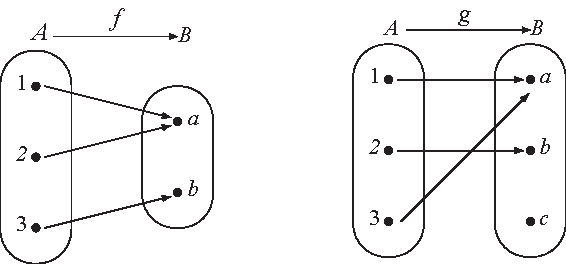
\includegraphics[width=\linewidth]{external/figps-arrow63-1new.pdf}
\end{image}%
\tcblower
\end{figureptx}%
Now let \(A = \left\{ {1,2,3} \right\}\), \(B = \left\{ {a,b,c,d} \right\}\), and \(C = \left\{ {s,t} \right\}\). Define%
\begin{center}%
{\tabularfont%
\begin{tabular}{ccc}
\multicolumn{1}{cB}{\(f\x A \to B\) by}&\multicolumn{1}{cB}{\(g\x A \to B\) by}&\(h\x A \to C\) by\tabularnewline[0pt]
\multicolumn{1}{cB}{\(f( 1 ) = a\)}&\multicolumn{1}{cB}{\(g( 1 ) = a\)}&\(h( 1 ) = s\)\tabularnewline[0pt]
\multicolumn{1}{cB}{\(f( 2 ) = b\)}&\multicolumn{1}{cB}{\(g( 2 ) = b\)}&\(h( 2 ) = t\)\tabularnewline[0pt]
\multicolumn{1}{cB}{\(f( 3 ) = c\)}&\multicolumn{1}{cB}{\(g( 3 ) = a\)}&\(h( 3 ) = s\)
\end{tabular}
}%
\end{center}%
\begin{divisionexercise}{1}{}{}{g:exercise:idm821376280}%
Which of these functions satisfy the following property for a function \(F\)? \begin{quote}%
For all \(x, y \in \text{ dom} ( F )\), if \(x \ne y\), then \(F(x) \ne F(y)\).\end{quote}
%
\end{divisionexercise}%
\begin{divisionexercise}{2}{}{}{g:exercise:idm821375640}%
Which of these functions satisfy the following property for a function \(F\)? \begin{quote}%
For all \(x, y \in \text{ dom} ( F )\), if \(F( x ) = F( y )\), then \(x = y\).\end{quote}
%
\end{divisionexercise}%
\begin{divisionexercise}{3}{}{}{g:exercise:idm820962840}%
Determine the range of each of these functions.%
\end{divisionexercise}%
\begin{divisionexercise}{4}{}{}{g:exercise:idm820960152}%
Which of these functions have their range equal to their codomain?%
\end{divisionexercise}%
\begin{divisionexercise}{5}{}{}{g:exercise:idm820960024}%
Which of the these functions satisfy the following property for a function \(F\)? \begin{quote}%
For all \(y\) in the codomain of \(F\), there exists an \(x \in \text{ dom} ( F )\) such that \(F( x ) = y\).\end{quote}
%
\end{divisionexercise}%
\end{worksheet-subsection}
%
%
\typeout{************************************************}
\typeout{Beginning Activity  Beginning Activity 2: Statements Involving Functions}
\typeout{************************************************}
%
\begin{worksheet-subsection}{Beginning Activity 2: Statements Involving Functions}{}{Beginning Activity 2: Statements Involving Functions}{}{}{x:worksheet:PA_functionstatements}
Let \(A\) and \(B\) be nonempty sets and let \(f\x A \to B\). In \hyperref[x:worksheet:PA_functionswithfinitedom]{Beginning Activity 1, p.\,\pageref{x:worksheet:PA_functionswithfinitedom}}, we determined whether or not certain functions satisfied some specified properties. These properties were written in the form of statements, and we will now examine these statements in more detail.%
\begin{divisionexercise}{1}{}{}{x:exercise:PA_functionstatements1}%
Consider the following statement: \begin{quote}%
For all \(x, y \in A\), if \(x \ne y\), then \(f ( x ) \ne f ( y )\).\end{quote}
%
\begin{enumerate}[font=\bfseries,label=(\alph*),ref=\alph*]
\item{}Write the contrapositive of this conditional statement.%
\item{}Write the negation of this conditional statement.%
\end{enumerate}
\end{divisionexercise}%
\begin{divisionexercise}{2}{}{}{x:exercise:PA_functionstatements2}%
Now consider the statement: \begin{quote}%
For all \(y \in B\), there exists an \(x \in A\) such that \(f ( x ) = y\).\end{quote}
 Write the negation of this statement.%
\end{divisionexercise}%
\begin{divisionexercise}{3}{}{}{x:exercise:PA_functionstatements3}%
Let \(g:\R \to \R\) be defined by \(g ( x ) = 5x + 3\), for all \(x \in \R\). Complete the following proofs of the following propositions about the function \(g\).%
\begin{descriptionlist}
\begin{dlimedium}{Propostion 1}{g:li:idm820950936}%
For all \(a,
b \in \R\), if \(g ( a ) = g ( b )\), then \(a = b\).%
\end{dlimedium}%
\begin{dlimedium}{Proof}{g:li:idm820946072}%
We let \(a, b \in \R\), and we assume that \(g ( a ) = g ( b )\) and will prove that \(a = b\). Since \(g(a) = g(b)\), we know that%
\begin{equation*}
5a + 3 = 5b + 3\text{.}
\end{equation*}
(Now prove that in this situation, \(a = b\).)%
\end{dlimedium}%
\end{descriptionlist}
%
\begin{descriptionlist}
\begin{dlimedium}{Proposition 2}{g:li:idm820945816}%
For all \(b \in \R\), there exists an \(a \in \R\) such that \(g ( a ) = b\).%
\end{dlimedium}%
\begin{dlimedium}{Proof}{g:li:idm820941080}%
We let \(b \in \R\). We will prove that there exists an \(a \in \R\) such that \(g ( a ) = b\) by constructing such an \(a\) in \(\R\). In order for this to happen, we need \(g(a) = 5a + 3 = b\).%
\par
(Now solve the equation for \(a\) and then show that for this real number \(a\), \(g ( a ) = b\).)%
\end{dlimedium}%
\end{descriptionlist}
%
\end{divisionexercise}%
\end{worksheet-subsection}
%
%
\typeout{************************************************}
\typeout{Subsection  Injections}
\typeout{************************************************}
%
\begin{subsectionptx}{Injections}{}{Injections}{}{}{g:subsection:idm820935192}
In previous sections and in \hyperref[x:worksheet:PA_functionswithfinitedom]{Beginning Activity 1, p.\,\pageref{x:worksheet:PA_functionswithfinitedom}}, we have seen examples of functions for which there exist different inputs that produce the same output. Using more formal notation, this means that there are functions \(f:A \to B\) for which there exist \(x_1 , x_2 \in A\) with \(x_1 \ne x_2\) and \(f( {x_1 } ) = f( {x_2 } )\). The work in the beginning activities was intended to motivate the following definition.%
\begin{assemblage}{Definition.}{x:assemblage:injection}%
Let \(f:A \to B\) be a function from the set \(A\) to the set \(B\). The function \(f\) is called an \terminology{injection} provided that \begin{quote}%
for all \(x_1 , x_2 \in A\), if \(x_1 \ne x_2\), then \(f( {x_1 } ) \ne f( {x_2 } )\).\end{quote}
 When \(f\) is an injection, we also say that \(f\) is a \terminology{one-to-one function}, or that \(f\) is an \terminology{injective function}.%
\end{assemblage}
Notice that the condition that specifies that a function \(f\) is an injection is given in the form of a conditional statement. As we shall see, in proofs, it is usually easier to use the contrapositive of this conditional statement. Although we did not define the term then, we have already written the contrapositive for the conditional statement in the definition of an injection in \hyperlink{x:exercise:PA_functionstatements1}{Exercise~{\xreffont 1}, p.\,\pageref{x:exercise:PA_functionstatements1}} of \hyperref[x:worksheet:PA_functionstatements]{Beginning Activity 2, p.\,\pageref{x:worksheet:PA_functionstatements}}. In that activity, we also wrote the negation of the definition of an injection. Following is a summary of this work giving the conditions for \(f\) being an injection or not being an injection.%
\begin{assemblage}{Let \(\boldsymbol{f\x A \to B}\).}{g:assemblage:idm820915224}%
``The function \(\boldsymbol{f}\) is an injection'' means that%
\begin{itemize}[label=\textbullet]
\item{}For all \(x_1 , x_2 \in A\), if \(x_1 \ne x_2\), then \(f( {x_1 } ) \ne f( {x_2 } )\); or%
\item{}For all \(x_1 , x_2 \in A\), if \(f( {x_1 } ) = f( {x_2 } )\), then \(x_1 = x_2\).%
\end{itemize}
%
\par
``The function \(\boldsymbol{f}\) is not an injection'' means that%
\begin{itemize}[label=\textbullet]
\item{}There exist \(x_1 , x_2 \in A\) such that \(x_1 \ne x_2\) and \(f( {x_1 } ) = f( {x_2 } )\).%
\end{itemize}
%
\end{assemblage}
\begin{inlineexercise}{Working with the Definition of an Injection.}{x:exercise:pr_injections}%
Now that we have defined what it means for a function to be an injection, we can see that in \hyperlink{x:exercise:PA_functionstatements3}{Exercise~{\xreffont 3}, p.\,\pageref{x:exercise:PA_functionstatements3}} of \hyperref[x:worksheet:PA_functionstatements]{Beginning Actiivty 2, p.\,\pageref{x:worksheet:PA_functionstatements}}, we proved that the function \(g\x \R \to \R\) is an injection, where \(g ( x ) = 5x + 3\) for all \(x \in \R\). Use the definition (or its negation) to determine whether or not the following functions are injections.%
\begin{enumerate}[font=\bfseries,label=(\alph*),ref=\alph*]
\item{}\(k:A \to B\), where \(A = \left\{a, b, c \right\}\), \(B = \left\{1, 2, 3, 4 \right\}\), and \(k (a) = 4\), \(k(b) = 1\), and \(k(c) = 3\).%
\item{}\(f:A \to C\), where \(A = \left\{a, b, c \right\}\), \(C = \left\{1, 2, 3\right\}\), and \(f(a) = 2\), \(f(b) = 3\), and \(f(c) = 2\).%
\item{}\(F: \Z \to \Z\) defined by \(F ( m ) = 3m + 2\) for all \(m \in \Z\)%
\item{}\(h: \R \to \R\) defined by \(h ( x ) = x^2 - 3x\) for all \(x \in \R\)%
\item{}\(R_5 = \{0, 1, 2, 3, 4 \}\) and \(s:R_5 \to R_5\) defined by \(s ( x ) = x^3 \pmod 5\) for all \(x \in R_5\).%
\space\hyperlink{g:solution:idm820901784-back}{[Solution]}\end{enumerate}
\end{inlineexercise}%
\end{subsectionptx}
%
%
\typeout{************************************************}
\typeout{Subsection  Surjections}
\typeout{************************************************}
%
\begin{subsectionptx}{Surjections}{}{Surjections}{}{}{g:subsection:idm820894616}
In previous sections and in \hyperref[x:worksheet:PA_functionswithfinitedom]{Beginning Activity 1, p.\,\pageref{x:worksheet:PA_functionswithfinitedom}}, we have seen that there exist functions \(f\x A \to B\) for which \(\text{ range} (f) = B\). This means that every element of \(B\) is an output of the function \(f\) for some input from the set \(A\). Using quantifiers, this means that for every \(y \in B\), there exists an \(x \in A\) such that \(f( x ) = y\) . One of the objectives of the beginning activities was to motivate the following definition.%
\begin{assemblage}{Definition.}{x:assemblage:surjection}%
Let \(f\x A \to B\) be a function from the set \(A\) to the set \(B\). The function \(f\) is called a \terminology{surjection} provided that the range of \(f\) equals the codomain of \(f\). This means that \begin{quote}%
for every \(y \in B\), there exists an \(x \in A\) such that \(f( x ) = y\).\end{quote}
 When \(f\) is a surjection, we also say that \(f\) is an \terminology{onto function} or that \(f\) maps \(\boldsymbol{A}\) \terminology{onto \(\boldsymbol{B}\)}. We also say that \(f\) is a \terminology{surjective function}.%
\end{assemblage}
One of the conditions that specifies that a function \(f\) is a surjection is given in the form of a universally quantified statement, which is the primary statement used in proving a function is (or is not) a surjection. Although we did not define the term then, we have already written the negation for the statement defining a surjection in \hyperlink{x:exercise:PA_functionstatements2}{Exercise~{\xreffont 2}, p.\,\pageref{x:exercise:PA_functionstatements2}} of \hyperref[x:worksheet:PA_functionstatements]{Beginning Activity 2, p.\,\pageref{x:worksheet:PA_functionstatements}}. We now summarize the conditions for \(f\) being a surjection or not being a surjection.%
\begin{assemblage}{Let \(\boldsymbol{f\x A \to B}\).}{g:assemblage:idm820875928}%
``The function \(\boldsymbol{f}\) is a surjection'' means that%
\begin{itemize}[label=\textbullet]
\item{}\(\text{ range} ( f ) = \text{ codom} ( f ) = B\); or%
\item{}For every \(y \in B\), there exists an \(x \in A\) such that \(f( x ) = y\).%
\end{itemize}
%
\par
``The function \(\boldsymbol{f}\) is not a surjection'' means that%
\begin{itemize}[label=\textbullet]
\item{}\(\text{ range} ( f ) \ne \text{ codom} ( f )\); or%
\item{}There exists a \(y \in B\) such that for all \(x \in A\), \(f( x ) \ne y\).%
\end{itemize}
%
\end{assemblage}
One other important type of function is when a function is both an injection and surjection. This type of function is called a bijection.%
\begin{assemblage}{Definition.}{x:assemblage:bijection}%
A \terminology{bijection} is a function that is both an injection and a surjection. If the function \(f\) is a bijection, we also say that \(f\) is \terminology{one-to-one and onto} and that \(f\) is a \terminology{bijective function}.%
\end{assemblage}
\begin{inlineexercise}{Working with the Definition of a Surjection.}{x:exercise:pr_functionswithfinitedom}%
Now that we have defined what it means for a function to be a surjection, we can see that in \hyperlink{x:exercise:PA_functionstatements3}{Exercise~{\xreffont 3}, p.\,\pageref{x:exercise:PA_functionstatements3}} of \hyperref[x:worksheet:PA_functionstatements]{Beginning Activity 2, p.\,\pageref{x:worksheet:PA_functionstatements}}, we proved that the function \(g: \R \to \R\) is a surjection, where \(g ( x ) = 5x + 3\) for all \(x \in \R\). Determine whether or not the following functions are surjections.%
\begin{enumerate}[font=\bfseries,label=(\alph*),ref=\alph*]
\item{}\(k\x A \to B\), where \(A = \left\{a, b, c \right\}\), \(B = \left\{1, 2, 3, 4 \right\}\), and \(k (a) = 4\), \(k(b) = 1\), and \(k(c) = 3\).%
\item{}\(f\x \R \to \R\) defined by \(f ( x ) = 3x + 2\) for all \(x \in \R\).%
\item{}\(F\x \Z \to \Z\) defined by \(F ( m ) = 3m + 2\) for all \(m \in \Z\).%
\item{}\(s:R_5 \to R_5\) defined by \(s ( x ) = x^3 \pmod 5\) for all \(x \in R_5\).%
\space\hyperlink{g:solution:idm820855192-back}{[Solution]}\end{enumerate}
\end{inlineexercise}%
\end{subsectionptx}
%
%
\typeout{************************************************}
\typeout{Subsection  The Importance of the Domain and Codomain}
\typeout{************************************************}
%
\begin{subsectionptx}{The Importance of the Domain and Codomain}{}{The Importance of the Domain and Codomain}{}{}{g:subsection:idm820853528}
The functions in the next two examples will illustrate why the domain and the codomain of a function are just as important as the rule defining the outputs of a function when we need to determine if the function is a surjection.%
\begin{example}{A Function that Is Neither an Injection nor a Surjection.}{x:example:E_domainandcodomain}%
Let \(f\x \mathbb{R} \to \mathbb{R}\) be defined by \(f( x ) = x^2  + 1\). Notice that%
\begin{equation*}
f( 2 ) = 5  \text{ and }  f( { - 2} ) = 5\text{.}
\end{equation*}
%
\par
This is enough to prove that the function \(f\) is not an injection since this shows that there exist two different inputs that produce the same output.%
\par
Since \(f( x ) = x^2 + 1\), we know that \(f( x ) \geq 1\) for all \(x \in \mathbb{R}\). This implies that the function \(f\) is not a surjection. For example, \(- 2\) is in the codomain of \(f\) and \(f( x ) \ne - 2\) for all \(x\) in the domain of \(f\).%
\end{example}
\begin{example}{A Function that Is Not an Injection but Is a Surjection.}{x:example:E_domainandcodomain2}%
Let \(T = \left\{ y \in \mathbb{R} \mid y \geq 1 \right\}\), and define \(F\x \mathbb{R} \to T\) by \(F( x ) = x^2 + 1\). As in \hyperref[x:example:E_domainandcodomain]{Example~{\xreffont\ref{x:example:E_domainandcodomain}}, p.\,\pageref{x:example:E_domainandcodomain}}, the function \(F\) is not an injection since \(F( 2 ) = F( { - 2} ) = 5\).%
\par
Is the function \(F\) a surjection? That is, does \(F\) map \(\mathbb{R}\) onto \(T\)? As in \hyperref[x:example:E_domainandcodomain]{Example~{\xreffont\ref{x:example:E_domainandcodomain}}, p.\,\pageref{x:example:E_domainandcodomain}}, we do know that \(F( x ) \geq 1\) for all \(x \in \mathbb{R}\).%
\par
To see if it is a surjection, we must determine if it is true that for every \(y \in T\), there exists an \(x \in \mathbb{R}\) such that \(F ( x ) = y\). So we choose \(y \in T\). The goal is to determine if there exists an \(x \in \mathbb{R}\) such that%
\begin{align*}
F( x ) \amp = y \text{ , or }\\
x^2  + 1 \amp = y\text{.}
\end{align*}
%
\par
One way to proceed is to work backward and solve the last equation (if possible) for \(x\). Doing so, we get%
\begin{align*}
x^2 \amp = y - 1\\
x = \sqrt {y - 1} \amp \text{   or   } x =  - \sqrt {y - 1}\text{.}
\end{align*}
%
\par
Now, since \(y \in T\), we know that \(y \geq 1\) and hence that \(y - 1 \geq 0\). This means that \(\sqrt {y - 1}  \in \mathbb{R}\). Hence, if we use \(x = \sqrt {y - 1}\), then \(x \in \mathbb{R}\), and%
\begin{align*}
F( x ) \amp = F\left( {\sqrt {y - 1} } \:\right)\\
\amp = \left( {\sqrt {y - 1} } \: \right)^2  + 1\\
\amp = ( {y - 1} ) + 1\\
\amp = y\text{.}
\end{align*}
%
\par
This proves that \(F\) is a surjection since we have shown that for all \(y \in T\), there exists an \(x \in \mathbb{R}\) such that \(F( x ) = y\). Notice that for each \(y \in T\), this was a constructive proof of the existence of an \(x \in \mathbb{R}\) such that \(F ( x ) = y\).%
\end{example}
\begin{paragraphs}{An Important Lesson.}{g:paragraphs:idm820825496}%
In \hyperref[x:example:E_domainandcodomain]{Example~{\xreffont\ref{x:example:E_domainandcodomain}}, p.\,\pageref{x:example:E_domainandcodomain}} and \hyperref[x:example:E_domainandcodomain2]{Example~{\xreffont\ref{x:example:E_domainandcodomain2}}, p.\,\pageref{x:example:E_domainandcodomain2}}, the same mathematical formula was used to determine the outputs for the functions. However, one function was not a surjection and the other one was a surjection. This illustrates the important fact that whether a function is surjective depends not only on the formula that defines the output of the function but also on the domain and codomain of the function.%
\end{paragraphs}%
\par
The next example will show that whether or not a function is an injection also depends on the domain of the function.%
\begin{example}{A Function that Is an Injection but Is Not a Surjection.}{x:example:E_domainandcodomain3}%
Let \(\mathbb{Z}^* = \left\{ { {x \in \mathbb{Z}} \mid x \geq 0} \right\} = 
\mathbb{N} \cup \left\{ 0 \right\}\). Define \(g\x \mathbb{Z}^* \to \mathbb{N}\) by \(g( x ) = x^2 + 1\). (Notice that this is the same formula used in \hyperref[x:example:E_domainandcodomain]{Example~{\xreffont\ref{x:example:E_domainandcodomain}}, p.\,\pageref{x:example:E_domainandcodomain}} and \hyperref[x:example:E_domainandcodomain2]{Example~{\xreffont\ref{x:example:E_domainandcodomain2}}, p.\,\pageref{x:example:E_domainandcodomain2}}.) Following is a table of values for some inputs for the function \(g\).%
\begin{center}%
{\tabularfont%
\begin{tabular}{cc}
\multicolumn{1}{cB}{\(x\)}&\(g ( x )\)\tabularnewline\hrulemedium
\multicolumn{1}{cB}{0}&1\tabularnewline\hrulemedium
\multicolumn{1}{cB}{1}&2\tabularnewline\hrulemedium
\multicolumn{1}{cB}{2}&5\tabularnewline\hrulemedium
\multicolumn{1}{cB}{3}&10\tabularnewline\hrulemedium
\multicolumn{1}{cB}{4}&17\tabularnewline\hrulemedium
\multicolumn{1}{cB}{5}&26
\end{tabular}
}%
\end{center}%
Notice that the codomain is \(\mathbb{N}\), and the table of values suggests that some natural numbers are not outputs of this function. So it appears that the function \(g\) is not a surjection.%
\par
To prove that \(g\) is not a surjection, pick an element of \(\N\) that does not appear to be in the range. We will use 3, and we will use a proof by contradiction to prove that there is no \(x\) in the domain \(\left( \Z^*\right)\) such that \(g( x ) = 3\). So we assume that there exists an \(x \in \Z^*\) with \(g( x ) = 3\). Then%
\begin{align*}
x^2  + 1 \amp = 3\\
x^2 \amp = 2\\
x \amp =  \pm \sqrt 2\text{.}
\end{align*}
%
\par
But this is not possible since \(\sqrt 2 \notin \mathbb{Z}^*\). Therefore, there is no \(x \in \mathbb{Z}^*\) with \(g( x ) = 3\). This means that for every \(x \in \mathbb{Z}^*\), \(g( x ) \ne 3\). Therefore, 3 is not in the range of \(g\), and hence \(g\) is not a surjection.%
\par
The table of values suggests that different inputs produce different outputs, and hence that \(g\) is an injection. To prove that \(g\) is an injection, assume that \(s, t \in \Z^*\) (the domain) with \(g( s ) = g( t )\). Then%
\begin{align*}
s^2  + 1 \amp = t^2  + 1\\
s^2  \amp = t^2\text{.}
\end{align*}
%
\par
Since \(s, t \in \mathbb{Z}^*\), we know that \(s \geq 0\text{ and } t \geq 0\). So the preceding equation implies that \(s = t\). Hence, \(g\) is an injection.%
\end{example}
\begin{paragraphs}{An Important Lesson.}{g:paragraphs:idm820804504}%
The functions in the three preceding examples all used the same formula to determine the outputs. The functions in \hyperref[x:example:E_domainandcodomain]{Example~{\xreffont\ref{x:example:E_domainandcodomain}}, p.\,\pageref{x:example:E_domainandcodomain}} and \hyperref[x:example:E_domainandcodomain2]{Example~{\xreffont\ref{x:example:E_domainandcodomain2}}, p.\,\pageref{x:example:E_domainandcodomain2}} are not injections but the function in \hyperref[x:example:E_domainandcodomain3]{Example~{\xreffont\ref{x:example:E_domainandcodomain3}}, p.\,\pageref{x:example:E_domainandcodomain3}} is an injection. This illustrates the important fact that whether a function is injective not only depends on the formula that defines the output of the function but also on the domain of the function.%
\end{paragraphs}%
\begin{inlineexercise}{The Importance of the Domain and Codomain.}{x:exercise:pr_domainandcodomain}%
Let \(\R^+ = \{ y \in \R \mid y > 0 \}\). Define \begin{quote}%
\(f \x \R \to \R\) by \(f(x) = e^{-x}\), for each \(x \in \R\), and\end{quote}
 \begin{quote}%
\(g \x \R \to \R^+\) by \(g(x) = e^{-x}\), for each \(x \in \R\).\end{quote}
 Determine if each of these functions is an injection or a surjection. Justify your conclusions.%
\par
Note: Before writing proofs, it might be helpful to draw the graph of \(y = e^{-x}\). A reasonable graph can be obtained using \(-3 \leq x \leq 3\) and \(-2 \leq y \leq 10\). Please keep in mind that the graph does not prove any conclusion, but may help us arrive at the correct conclusions, which will still need proof.%
\space\hyperlink{g:solution:idm820797592-back}{[Solution]}\end{inlineexercise}%
\end{subsectionptx}
%
%
\typeout{************************************************}
\typeout{Subsection  Working with a Function of Two Variables}
\typeout{************************************************}
%
\begin{subsectionptx}{Working with a Function of Two Variables}{}{Working with a Function of Two Variables}{}{}{g:subsection:idm820788632}
It takes time and practice to become efficient at working with the formal definitions of injection and surjection. As we have seen, all parts of a function are important (the domain, the codomain, and the rule for determining outputs). This is especially true for functions of two variables.%
\par
For example, we define \(f\x \mathbb{R} \times \mathbb{R} \to \mathbb{R} \times \mathbb{R}\) by%
\begin{equation*}
f( {a, b} ) = ( {2a + b, a - b} )  \text{ for all } ( {a, b} ) \in \R \times \R\text{.}
\end{equation*}
%
\par
Notice that both the domain and the codomain of this function are the set \(\mathbb{R} \times \mathbb{R}\). Thus, the inputs and the outputs of this function are ordered pairs of real numbers. For example,%
\begin{equation*}
f( {1, 1} ) = ( {3, 0} )  \text{ and }   f( { - 1, 2} ) = ( {0,  - 3} ). \\
\end{equation*}
%
\par
To explore whether or not \(f\) is an injection, we assume that \(( {a, b} ) \in \mathbb{R} \times \mathbb{R}\), \(( {c, d} ) \in \mathbb{R} \times \mathbb{R}\), and \(f( {a, b} ) = f( {c, d} )\). This means that%
\begin{equation*}
( {2a + b, a - b} ) = ( {2c + d, c - d} )\text{.}
\end{equation*}
%
\par
Since this equation is an equality of ordered pairs, we see that%
\begin{align*}
2a + b \amp = 2c + d\text{, and }\\
a - b \amp = c - d\!\text{.}
\end{align*}
%
\par
By adding the corresponding sides of the two equations in this system, we obtain \(3a = 3c\) and hence, \(a = c\). Substituting \(a = c\) into either equation in the system give us \(b = d\). Since \(a = c\) and \(b = d\), we conclude that%
\begin{equation*}
( {a, b} ) = ( {c, d} )\text{.}
\end{equation*}
%
\par
Hence, we have shown that if \(f( {a, b} ) = f( {c, d} )\), then \(( {a, b} ) = ( {c, d} )\). Therefore, \(f\) is an injection.%
\par
Now, to determine if \(f\) is a surjection, we let \(( {r, s} ) \in \mathbb{R} \times \mathbb{R}\), where \(( {r, s} )\) is considered to be an arbitrary element of the codomain of the function \(f\). Can we find an ordered pair \(( {a, b} ) \in \mathbb{R} \times \mathbb{R}\) such that \(f( {a, b} ) = ( {r, s} )\)? Working backward, we see that in order to do this, we need%
\begin{equation*}
( {2a + b, a - b} ) = ( {r, s} )\text{.}
\end{equation*}
%
\par
That is, we need%
\begin{equation*}
2a + b = r  \text{ and }      a - b = s\text{.}
\end{equation*}
%
\par
Solving this system for \(a\) and \(b\) yields%
\begin{equation*}
a = \frac{{r + s}}{3} \text{ and }  b = \frac{{r - 2s}}{3}\text{.}
\end{equation*}
%
\par
Since \(r, s \in \mathbb{R}\), we can conclude that \(a \in \mathbb{R}\) and \(b \in \mathbb{R}\) and hence that \(( {a, b} ) \in \mathbb{R} \times \mathbb{R}\). We now need to verify that for these values of \(a\) and \(b\), we get \(f( {a, b} ) = ( {r, s} )\). So%
\begin{align*}
f( {a, b} ) \amp = f\!\left( {\frac{{r + s}}{3}, \frac{{r - 2s}}{3}} \right)\\
\amp = \left( {2\left( {\frac{{r + s}}{3}} \right) + \frac{{r - 2s}}{3}, 
\frac{{r + s}}{3} - \frac{{r - 2s}}{3}} \right)\\
\amp = \left( {\frac{{2r + 2s + r - 2s}}{3}, \frac{{r + s - r + 2s}}{3}} \right)\\
\amp = ( {r, s} )
\end{align*}
%
\par
This proves that for all \(( {r, s} ) \in \mathbb{R} \times \mathbb{R}\), there exists \(( {a, b} ) \in \mathbb{R} \times \mathbb{R}\) such that \(f( {a, b} ) = ( {r, s} )\). Hence, the function \(f\) is a surjection. Since \(f\) is both an injection and a surjection, it is a bijection.%
\begin{inlineexercise}{A Function of Two Variables.}{x:exercise:pr_function2variables}%
Let \(g \x \R \times \R \to \R\) be defined by \(g(x, y) = 2x + y\), for all \((x, y) \in \R \times \R\).%
\par
Note: Be careful! One major difference between this function and the previous example is that for the function \(g\), the codomain is \(\R\), not \(\R \times \R\). It is a good idea to begin by computing several outputs for several inputs (and remember that the inputs are ordered pairs).%
\begin{enumerate}[font=\bfseries,label=(\alph*),ref=\alph*]
\item{}Notice that the ordered pair \((1, 0) \in \R \times \R\). That is, \((1, 0)\) is in the domain of \(g\). Also notice that \(g(1, 0) = 2\). Is it possible to find another ordered pair \((a, b) \in \R \times \R\) such that \(g(a, b) = 2\)?%
\space\hyperlink{g:solution:idm820764952-back}{[Solution]}\item{}Let \(z \in \R\). Then \((0, z) \in \R \times \R\) and so \((0, z) \in \text{ dom} (g)\). Now determine \(g(0, z)\).%
\space\hyperlink{g:solution:idm820750360-back}{[Solution]}\item{}Is the function \(g\) an injection? Is the function \(g\) a surjection? Justify your conclusions.%
\space\hyperlink{g:solution:idm820754968-back}{[Solution]}\end{enumerate}
\end{inlineexercise}%
\end{subsectionptx}
%
%
\typeout{************************************************}
\typeout{Exercises  Exercises}
\typeout{************************************************}
%
\begin{exercises-subsection}{Exercises}{}{Exercises}{}{}{g:exercises:idm820742296}
\begin{divisionexercise}{1}{}{}{g:exercise:idm820747800}%
Draw an arrow diagram that%
\begin{enumerate}[font=\bfseries,label=(\alph*),ref=\alph*]
\item{}represents a function that is an injection but is not a surjection.%
\item{}represents a function that is an injection and is a surjection.%
\item{}represents a function that is not an injection and is not a surjection.%
\item{}represents a function that is not an injection but is a surjection.%
\item{}represents a function that is not a bijection.%
\end{enumerate}
\end{divisionexercise}%
\begin{divisionexercise}{2}{}{}{x:exercise:exer_sec63-mod5function}%
We know \(R_5 = \left\{ {0, 1, 2, 3, 4} \right\}\) and \(R_6 = \left\{ {0, 1, 2, 3, 4, 5} \right\}\). For each of the following functions, determine if the function is an injection and determine if the function is a surjection. Justify all conclusions.%
\begin{enumerate}[font=\bfseries,label=(\alph*),ref=\alph*]
\item{}\(f\x R_5 \to R_5\) by \(f( x ) = x^2 + 4 \pmod 5\), for all \(x \in R_5\)%
\space\hyperlink{g:answer:idm820745624-back}{[Answer]}\item{}\(g\x R_6 \to R_6\) by \(g( x ) = x^2 + 4 \pmod 6\), for all \(x \in R_6\)%
\item{}\(F\x R_5 \to R_5\) by \(F( x ) = x^3 + 4 \pmod 5\), for all \(x \in R_5\)%
\space\hyperlink{g:answer:idm820740632-back}{[Answer]}\end{enumerate}
\end{divisionexercise}%
\begin{divisionexercise}{3}{}{}{x:exercise:exer_sec63-5}%
For each of the following functions, determine if the function is an injection and determine if the function is a surjection. Justify all conclusions.%
\begin{enumerate}[font=\bfseries,label=(\alph*),ref=\alph*]
\item{}\(f\x\mathbb{Z} \to \mathbb{Z}\) defined by \(f( x ) = 3x + 1\), for all \(x \in \Z\).%
\space\hyperlink{g:answer:idm820730520-back}{[Answer]}\item{}\(F\x\mathbb{Q} \to \mathbb{Q}\) defined by \(F( x ) = 3x + 1\), for all \(x \in \Q\).%
\space\hyperlink{g:answer:idm820728600-back}{[Answer]}\item{}\(g\x\mathbb{R} \to \mathbb{R}\) defined by \(g( x ) = x^3\), for all \(x \in \R\).%
\item{}\(G \x\mathbb{Q} \to \mathbb{Q}\) defined by \(G( x ) = x^3\), for all \(x \in \Q\).%
\item{}\(k \x \R \to \R\) defined by \(k(x) = e^{-x^2}\), for all \(x \in \R\).%
\item{}\(K\x \R^* \to \R\) defined by \(K(x) = e^{-x^2}\), for all \(x \in \R^*\).%
\par
Note: \(\R^* = \left\{ x \in \R \mid x \geq 0 \right\}\).%
\item{}\(K_1 \x \R^* \to T\) defined by \(K_1(x) = e^{-x^2}\), for all \(x \in \R^*\), where \(T = \left\{ y \in \R \mid 0 \lt y \leq 1 \right\}\).%
\item{}\(h \x\R \to \R\) defined by \(h ( x ) = \dfrac{2x}{x^2 + 4}\), for all \(x \in \R\).%
\space\hyperlink{g:answer:idm820714136-back}{[Answer]}\item{}\(H \x \{x \in \R \mid x \geq 0 \} \to \left\{ y \in \R \left| 0 
\leq y \leq \dfrac{1}{2} \right. \right\}\) defined by \(H ( x ) = \dfrac{2x}{x^2 + 4}\), for all \(x \in \{x \in \R \mid x \geq 0 \}\).%
\end{enumerate}
\end{divisionexercise}%
\begin{divisionexercise}{4}{}{}{x:exercise:exer_forexample}%
For each of the following functions, determine if the function is a bijection. Justify all conclusions.%
\begin{enumerate}[font=\bfseries,label=(\alph*),ref=\alph*]
\item{}\(F\x\mathbb{R} \to \mathbb{R}\) defined by \(F( x ) = 5x + 3\), for all \(x \in \mathbb{R}\).%
\space\hyperlink{g:answer:idm820965912-back}{[Answer]}\item{}\(G\x\Z \to \Z\) defined by \(G( x ) = 5x + 3\), for all \(x \in \Z\).%
\space\hyperlink{g:answer:idm820698024-back}{[Answer]}\item{}\(f\x ( \R -\left\{ 4 \right\} ) \to \R\) defined by \(f ( x ) = \dfrac{3x}{x - 4}\), for all \(x \in \left( \R - \{ 4 \} \right)\).%
\item{}\(g\x ( \R -\left\{ 4 \right\} ) \to ( \R - \left\{ 3 \right\} )\) defined by \(g ( x ) = \dfrac{3x}{x - 4}\), for all \textbackslash{}linebreak\(x \in \left( \R - \{ 4 \} \right)\).%
\end{enumerate}
\end{divisionexercise}%
\begin{divisionexercise}{5}{}{}{x:exercise:exer_sec63-sumdivisors}%
\index{sum of divisors function}%
Let \(s\x\mathbb{N} \to \mathbb{N}\), where for each \(n \in \mathbb{N}\), \(s( n )\) is the sum of the distinct natural number divisors of \(n\). This is the \terminology{sum of the divisors function} that was introduced in \hyperref[x:worksheet:PA_otherfunctions]{Beginning Activity 2, p.\,\pageref{x:worksheet:PA_otherfunctions}} from \hyperref[x:section:S_introfunctions]{Section~{\xreffont\ref{x:section:S_introfunctions}}, p.\,\pageref{x:section:S_introfunctions}}. Is \(s\) an injection? Is \(s\) a surjection? Justify your conclusions.%
\end{divisionexercise}%
\begin{divisionexercise}{6}{}{}{x:exercise:exer_sec63-numdivisors}%
\index{number of divisors function}%
Let \(d\x\mathbb{N} \to \mathbb{N}\), where \(d( n )\) is the number of natural number divisors of \(n\). This is the \terminology{number of divisors function} introduced in \hyperlink{x:exercise:exer_numberofdivisors}{Exercise~{\xreffont 6}, p.\,\pageref{x:exercise:exer_numberofdivisors}} from \hyperref[x:section:S_introfunctions]{Section~{\xreffont\ref{x:section:S_introfunctions}}, p.\,\pageref{x:section:S_introfunctions}}. Is the function \(d\) an injection? Is the function \(d\) a surjection? Justify your conclusions.%
\end{divisionexercise}%
\begin{divisionexercise}{7}{}{}{x:exercise:exer_sec63-9}%
\index{birthday function}%
In \hyperref[x:worksheet:PA_otherfunctions]{Beginning Activity 2, p.\,\pageref{x:worksheet:PA_otherfunctions}} from \hyperref[x:section:S_introfunctions]{Section~{\xreffont\ref{x:section:S_introfunctions}}, p.\,\pageref{x:section:S_introfunctions}}, we introduced the \terminology{birthday function}. Is the birthday function an injection? Is it a surjection? Justify your conclusions.%
\space\hyperlink{g:answer:idm820683688-back}{[Answer]}\end{divisionexercise}%
\begin{divisionexercise}{8}{}{}{x:exercise:exer_sec63-10}%
Complete the following. Justify your conclusions.%
\begin{enumerate}[font=\bfseries,label=(\alph*),ref=\alph*]
\item{}Let \(f\x\mathbb{Z} \times \mathbb{Z} \to \mathbb{Z}\) be defined by \(f( {m, n} ) = 2m + n\). Is the function \(f\) an injection? Is the function \(f\) a surjection?%
\item{}Let \(g\x\mathbb{Z} \times \mathbb{Z} \to \mathbb{Z}\) be defined by \(g( {m, n} ) = 6m + 3n\). Is the function \(g\) an injection? Is the function \(g\) a surjection?%
\end{enumerate}
\end{divisionexercise}%
\begin{divisionexercise}{9}{}{}{x:exercise:exer_sec63-11}%
Complete the following. Justify your conclusions.%
\begin{enumerate}[font=\bfseries,label=(\alph*),ref=\alph*]
\item{}Let \(f\x\mathbb{R} \times \mathbb{R} \to \mathbb{R} \times \mathbb{R}\) be defined by \(f( {x, y} ) = ( {2x, x + y} )\). Is the function \(f\) an injection? Is the function \(f\) a surjection?%
\space\hyperlink{g:answer:idm820668200-back}{[Answer]}\item{}Let \(g\x\mathbb{Z} \times \mathbb{Z} \to \mathbb{Z} \times \mathbb{Z}\) be defined by \(g( {x, y} ) = ( {2x, x + y} )\). Is the function \(g\) an injection? Is the function \(g\) a surjection?%
\space\hyperlink{g:answer:idm820652200-back}{[Answer]}\end{enumerate}
\end{divisionexercise}%
\begin{divisionexercise}{10}{}{}{g:exercise:idm820658728}%
Let \(f\x\R \times \R \to \R\) be the function defined by \(f (x, y ) = -x^2y+3y\), for all \((x, y ) \in \R \times \R\). Is the function \(f\) an injection? Is the function \(f\) a surjection? Justify your conclusions.%
\end{divisionexercise}%
\begin{divisionexercise}{11}{}{}{g:exercise:idm820654376}%
Let \(g\x\R \times \R \to \R\) be the function defined by \(g (x, y ) = ( x^3 + 2) \sin y\), for all \((x, y ) \in \R \times \R\). Is the function \(g\) an injection? Is the function \(g\) a surjection? Justify your conclusions.%
\end{divisionexercise}%
\begin{divisionexercise}{12}{}{}{g:exercise:idm820646312}%
Let \(A\) be a nonempty set. The \terminology{identity function on the set \(\boldsymbol{A}\)}, \index{identity function} denoted by \(I_A\), is the function \(I_A \x A \to A\) defined by \(I_A ( x ) = x\) for every \(x\) in \(A\). Is \(I_A\) an injection? Is \(I_A\) a surjection? Justify your conclusions.%
\end{divisionexercise}%
\begin{divisionexercise}{13}{}{}{g:exercise:idm820646440}%
\index{projection function}%
Let  \(A\)  and  \(B\)  be two nonempty sets. Define%
\begin{equation*}
p_1 \x A \times B \to A \text{ by }   p_1 ( {a, b} ) = a
\end{equation*}
for every  \(( {a, b} ) \in A \times B\). This is the \terminology{first projection function} introduced in \hyperlink{x:exercise:sym_projfunc}{Exercise~{\xreffont 5}, p.\,\pageref{x:exercise:sym_projfunc}} in \hyperref[x:section:S_moreaboutfunctions]{Section~{\xreffont\ref{x:section:S_moreaboutfunctions}}, p.\,\pageref{x:section:S_moreaboutfunctions}}.%
\begin{enumerate}[font=\bfseries,label=(\alph*),ref=\alph*]
\item{}Is the function \(p_1\) a surjection? Justify your conclusion.%
\item{}If \(B = \left\{ b \right\}\), is the function \(p_1\) an injection? Justify your conclusion.%
\item{}Under what condition(s) is the function \(p_1\) not an injection? Make a conjecture and prove it.%
\end{enumerate}
\end{divisionexercise}%
\begin{divisionexercise}{14}{}{}{g:exercise:idm820636712}%
Define \(f:\N \to \Z\) as follows: For each \(n \in \N\),%
\begin{equation*}
f(n) = \dfrac{1 + (-1)^n (2n - 1)}{4}\text{.}
\end{equation*}
Is the function \(f\) an injection? Is the function \(f\) a surjection? Justify your conclusions.%
\par
Suggestions: Start by calculating several outputs for the function before you attempt to write a proof. In exploring whether or not the function is an injection, it might be a good idea to use cases based on whether the inputs are even or odd. In exploring whether \(f\) is a surjection, consider using cases based on whether the output is positive or less than or equal to zero.%
\end{divisionexercise}%
\begin{divisionexercise}{15}{}{}{g:exercise:idm820643240}%
Let \(C\) be the set of all real functions that are continuous on the closed interval \(\left[ 0, 1 \right]\). Define the function \(A\x C \to \mathbb{R}\) as follows: For each \(f \in C\),%
\begin{equation*}
A ( f ) = \int_0^1 {f( x ) \, dx}\text{.}
\end{equation*}
Is the function \(A\) an injection? Is it a surjection? Justify your conclusions.%
\end{divisionexercise}%
\begin{divisionexercise}{16}{}{}{g:exercise:idm820634408}%
Let \(A = \left\{ ( m, n ) \mid m \in \mathbb{Z}, n \in \mathbb{Z}, \text{ and } n \ne 0 \right\}\). Define \(f\x A \to \mathbb{Q}\) as follows: \begin{quote}%
For each \(( m, n ) \in A\), \(f ( m, n ) = \dfrac{m+n}{n}\).\end{quote}
%
\begin{enumerate}[font=\bfseries,label=(\alph*),ref=\alph*]
\item{}Is the function \(f\) an injection? Justify your conclusion.%
\item{}Is the function \(f\) a surjection? Justify your conclusion.%
\end{enumerate}
\end{divisionexercise}%
\begin{divisionexercise}{17}{Evaluation of Proofs.}{}{g:exercise:idm820629544}%
See the instructions for \hyperlink{x:exercise:exer_proofeval}{Exercise~{\xreffont 19}, p.\,\pageref{x:exercise:exer_proofeval}} from \hyperref[x:section:S_directproof]{Section~{\xreffont\ref{x:section:S_directproof}}, p.\,\pageref{x:section:S_directproof}}.%
\begin{enumerate}[font=\bfseries,label=(\alph*),ref=\alph*]
\item{}%
\begin{descriptionlist}
\begin{dlinarrow}{Proposition}{g:li:idm820619432}%
Propostion: The function \(f\x\R \times \R \to \R \times \R\) defined by \(f( {x, y} ) = ( {2x + y, x - y} )\) is an injection.%
\end{dlinarrow}%
\begin{dlinarrow}{Proof}{g:li:idm820622504}%
For each \((a, b)\) and \((c, d)\) in \(\R \times \R\), if \(f(a, b) = f(c, d)\), then%
\begin{equation*}
(2a + b, a - b) = (2c + d, c - d)\text{.}
\end{equation*}
%
\par
We will use systems of equations to prove that \(a = c\) and \(b = d\).%
\begin{align*}
2a + b \amp = 2c + d\\
a - b \amp =  c - d\\
3a  \amp = 3c\\
a  \amp = c
\end{align*}
%
\par
Since \(a = c\), we see that%
\begin{equation*}
(2c + b, c - b) = (2c + d, c - d)\text{.}
\end{equation*}
%
\par
So \(b = d\). Therefore, we have proved that the function \(f\) is an injection.%
\end{dlinarrow}%
\end{descriptionlist}
%
\item{}%
\begin{descriptionlist}
\begin{dlinarrow}{Proposition}{g:li:idm820615208}%
The function \(f\x\R \times \R \to \R \times \R\) defined by \(f( {x, y} ) = ( {2x + y, x - y} )\) is a surjection.%
\end{dlinarrow}%
\begin{dlinarrow}{Proof}{g:li:idm820617896}%
We need to find an ordered pair such that \(f(x, y) = (a, b)\) for each \((a, b)\) in \(\R \times \R\). That is, we need \((2x + y, x - y) = (a, b)\), or%
\begin{equation*}
2x + y = a \qquad \text{ and }  \qquad x - y = b\text{.}
\end{equation*}
%
\par
Treating these two equations as a system of equations and solving for \(x\) and \(y\), we find that%
\begin{equation*}
x = \frac{a + b}{3} \qquad \text{ and }  \qquad y = \frac{a - 2b}{3}\text{.}
\end{equation*}
%
\par
Hence, \(x\) and \(y\) are real numbers, \((x, y) \in \R \times \R\), and%
\begin{align*}
f(x, y) \amp = f \left( \frac{a + b}{3}, \frac{a - 2b}{3} \right)\\
\amp = \left(2 \left( \frac{a + b}{3} \right) + \frac{a - 2b}{3}, 
\frac{a + b}{3} - \frac{a - 2b}{3} \right)\\
\amp = \left( \frac{2a + 2b + a - 2b}{3}, \frac{a + b - a + 2b}{3} \right)\\
\amp = \left( \frac{3a}{3}, \frac{3b}{3} \right)\\
\amp = (a, b)\text{.}
\end{align*}
%
\par
Therefore, we have proved that for every \((a, b) \in \R \times \R\), there exists an \((x, y) \in \R \times \R\) such that \(f(x, y) = (a, b)\). This proves that the function \(f\) is a surjection.%
\end{dlinarrow}%
\end{descriptionlist}
%
\end{enumerate}
\end{divisionexercise}%
\begin{activity}{Piecewise Defined Functions.}{x:activity:exer_piecewisefunction}%
\index{function!piecewise defined}%
\index{piecewise defined function}%
We often say that a function is a \terminology{piecewise defined function} if it has different rules for determining the output for different parts of its domain. For example, we can define a function \(f\x\R \to \R\) by giving a rule for calculating \(f(x)\) when \(x \geq 0\) and giving a rule for calculating \(f(x)\) when \(x \lt  0\) as follows:%
\begin{equation*}
f(x) = \begin{cases}x^2 + 1,    \amp   \text{ if \(x \geq 0\); }  \\ x - 1      \amp   \text{ if \(x \lt  0\). } \end{cases}
\end{equation*}
%
\begin{enumerate}[font=\bfseries,label=(\alph*),ref=\alph*]
\item{}Sketch a graph of the function \(f\). Is the function \(f\) an injection? Is the function \(f\) a surjection? Justify your conclusions.%
\item{}For each of the following functions, determine if the function is an injection and determine if the function is a surjection.  Justify all conclusions.%
\begin{enumerate}[font=\bfseries,label=(\roman*),ref=\theenumi.\roman*]
\item{}\(g\x[0, 1] \to (0, 1)\) by%
\begin{equation*}
g(x) = \begin{cases}0.8, \amp   \text{ if \(x = 0\); }  \\ 0.5 x,    \amp   
\text{ if \(0 \lt  x \lt  1\); }  \\ 0.6  \amp   \text{ if \(x = 1\). } \end{cases}
\end{equation*}
%
\item{}\(h\x\Z \to \left\{ 0, 1 \right\}\) by%
\begin{equation*}
h(x) = \begin{cases}0,  \amp  \text{ if \(x\) is even; }  \\ 1,  \amp  
\text{ if \(x\) is odd. } \end{cases}
\end{equation*}
%
\end{enumerate}
\end{enumerate}
\end{activity}%
\begin{activity}{Functions Whose Domain is \(\boldsymbol{\mathcal{M}_2(\R)}\).}{x:activity:func_domain_m2r}%
Let \(\mathcal{M}_2 ( \R )\) represent the set of all 2 by 2 matrices over \(\mathbb{R}\).%
\begin{enumerate}[font=\bfseries,label=(\alph*),ref=\alph*]
\item\label{x:task:sym_detfunc}\index{determinant}%
\label{g:notation:idm820587432} Define  \(\det \x\mathcal{M}_2( \R ) \to \mathbb{R}\) by%
\begin{equation*}
\det \left[ {\begin{array}{*{20}c} a \amp  b  \\ c \amp  d \end{array}  } \right] = ad - bc\text{.}
\end{equation*}
This is the \terminology{determinant function} introduced in \hyperlink{x:exercise:sym_determinant}{Exercise~{\xreffont 9}, p.\,\pageref{x:exercise:sym_determinant}} from \hyperref[x:section:S_moreaboutfunctions]{Section~{\xreffont\ref{x:section:S_moreaboutfunctions}}, p.\,\pageref{x:section:S_moreaboutfunctions}}. Is the determinant function an injection? Is the determinant function a surjection? Justify your conclusions.%
\item\label{x:task:sym_tranfunc}\index{transpose}%
Define \(\text{ tran } \x\mathcal{M}_2( \R ) \to \mathcal{M}_2 ( \R )\) by%
\begin{equation*}
\text{ tran } \left[ {\begin{array}{*{20}c} a \amp  b  \\ c \amp  d \end{array}  } 
\right] = A^T  = \left[ {\begin{array}{*{20}c} a \amp  c  \\ b \amp  d \end{array}  } \right]\text{.}
\end{equation*}
This is the \terminology{transpose function} introduced in \hyperlink{x:exercise:sym_transpose}{Exercise~{\xreffont 10}, p.\,\pageref{x:exercise:sym_transpose}} from \hyperref[x:section:S_moreaboutfunctions]{Section~{\xreffont\ref{x:section:S_moreaboutfunctions}}, p.\,\pageref{x:section:S_moreaboutfunctions}}. Is the transpose function an injection? Is the transpose function a surjection? Justify your conclusions.%
\item\label{x:task:sym_detfunc2}Define \(F \x\mathcal{M}_2( \R ) \to \mathbb{R}\) by%
\begin{equation*}
F \left[ {\begin{array}{*{20}c} a \amp  b  \\ c \amp  d \end{array}  } \right] = a^2 + d^2 - b^2 - c^2\text{.}
\end{equation*}
Is the function \(F\) an injection? Is the function \(F\) a surjection? Justify your conclusions.%
\end{enumerate}
\end{activity}%
\end{exercises-subsection}
\end{sectionptx}
%
%
\typeout{************************************************}
\typeout{Section 6.4 Composition of Functions}
\typeout{************************************************}
%
\begin{sectionptx}{Composition of Functions}{}{Composition of Functions}{}{}{x:section:S_compositionoffunctions}
%
%
\typeout{************************************************}
\typeout{Beginning Activity  Beginning Activity 1: Constructing a New Function}
\typeout{************************************************}
%
\begin{worksheet-subsection}{Beginning Activity 1: Constructing a New Function}{}{Beginning Activity 1: Constructing a New Function}{}{}{x:worksheet:PA_compositionintro}
Let \(A = \left\{ {a, b, c, d} \right\}\), \(B = \left\{ {p, q, r} \right\}\), and \(C = \left\{ {s, t, u, v} \right\}\). The arrow diagram in \hyperref[x:figure:fig_preview64]{Figure~{\xreffont\ref{x:figure:fig_preview64}}, p.\,\pageref{x:figure:fig_preview64}} shows two functions: \(f\x A \to B\) and \(g\x B \to C\).%
\par
Notice that if \(x \in A\), then \(f(x) \in B\). Since \(f(x) \in B\), we can apply the function \(g\) to \(f(x)\), and we obtain \(g(f(x))\), which is an element of \(C\).%
\par
Using this process, determine \(g(f(a))\), \(g ( f(b) )\), \(g ( f(c) )\), and \(g ( f(d) )\). Then explain how we can use this information to define a function from \(A\) to \(C\).%
\begin{figureptx}{Arrow Diagram Showing Two Functions}{x:figure:fig_preview64}{}%
\begin{image}{0.3}{0.4}{0.3}%
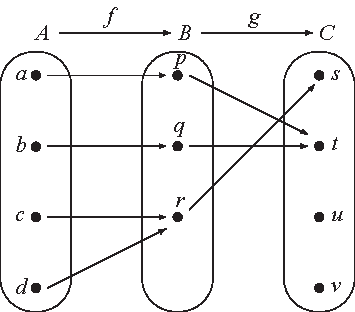
\includegraphics[width=\linewidth]{external/figps-prev641.pdf}
\end{image}%
\tcblower
\end{figureptx}%
\end{worksheet-subsection}
%
%
\typeout{************************************************}
\typeout{Beginning Activity  Beginning Activity 2: Verbal Descriptions of Functions}
\typeout{************************************************}
%
\begin{worksheet-subsection}{Beginning Activity 2: Verbal Descriptions of Functions}{}{Beginning Activity 2: Verbal Descriptions of Functions}{}{}{x:worksheet:PA_verbaldescriptions}
The outputs of most real functions we have studied in previous mathematics courses have been determined by mathematical expressions. In many cases, it is possible to use these expressions to give step-by-step verbal descriptions of how to compute the outputs. For example, if%
\begin{equation*}
f\x \mathbb{R} \to \mathbb{R}\text{  is defined by  } f( x ) = ( {3x + 2} )^3\text{,}
\end{equation*}
we could describe how to compute the outputs as follows:%
\begin{center}%
{\tabularfont%
\begin{tabular}{lll}
\multicolumn{1}{lB}{\textbf{Step}}&\multicolumn{1}{lB}{\textbf{Verbal Description}}&\textbf{Symbolic Result}\tabularnewline\hrulemedium
\multicolumn{1}{lB}{1}&\multicolumn{1}{lB}{Choose an input.}&\(x\)\tabularnewline\hrulemedium
\multicolumn{1}{lB}{2}&\multicolumn{1}{lB}{Multiply by 3.}&\(3x\)\tabularnewline\hrulemedium
\multicolumn{1}{lB}{3}&\multicolumn{1}{lB}{Add 2.}&\(3x + 2\)\tabularnewline\hrulemedium
\multicolumn{1}{lB}{4}&\multicolumn{1}{lB}{Cube the result.}&\(( {3x + 2} )^3\)
\end{tabular}
}%
\end{center}%
Complete step-by-step verbal descriptions for each of the following functions.%
\begin{divisionexercise}{1}{}{}{g:exercise:idm820566056}%
\(f\x \mathbb{R} \to \mathbb{R}\) by \(f( x ) = \sqrt {3x^2 + 2}\), for each \(x \in \R\).%
\end{divisionexercise}%
\begin{divisionexercise}{2}{}{}{g:exercise:idm820563112}%
\(g\x \mathbb{R} \to \mathbb{R}\) by \(g( x ) = \sin \! \left( {3x^2 + 2} \right)\), for each \(x \in \R\).%
\end{divisionexercise}%
\begin{divisionexercise}{3}{}{}{g:exercise:idm820561576}%
\(h\x \mathbb{R} \to \mathbb{R}\) by \(h( x ) = e^{3x^2 + 2}\), for each \(x \in \R\).%
\end{divisionexercise}%
\begin{divisionexercise}{4}{}{}{g:exercise:idm820560680}%
\(G\x \R \to \R\) by \(G(x) = \ln ( x^4 + 3 )\), for each \(x \in \R\).%
\end{divisionexercise}%
\begin{divisionexercise}{5}{}{}{g:exercise:idm820554408}%
\(k \x \R \to \R\) by \(k(x) = \sqrt[3]{\dfrac{\sin (4x + 3)}{x^2 + 1}}\), for each \(x \in \R\).%
\end{divisionexercise}%
\end{worksheet-subsection}
%
%
\typeout{************************************************}
\typeout{Subsection  Composition of Functions}
\typeout{************************************************}
%
\begin{subsectionptx}{Composition of Functions}{}{Composition of Functions}{}{}{x:subsection:sub-compfunc}
There are several ways to combine two existing functions to create a new function. For example, in calculus, we learned how to form the product and quotient of two functions and then how to use the product rule to determine the derivative of a product of two functions and the quotient rule to determine the derivative of the quotient of two functions.%
\par
The chain rule in calculus was used to determine the derivative of the composition of two functions, and in this section, we will focus only on the composition of two functions. We will then consider some results about the compositions of injections and surjections.%
\par
The basic idea of function composition is that when possible, the output of a function \(f\) is used as the input of a function \(g\). This can be referred to as ``\(f\) followed by \(g\)'' and is called the composition of \(f\) and \(g\). In previous mathematics courses, we used this idea to determine a formula for the composition of two real functions.%
\par
For example, if%
\begin{equation*}
f( x ) = 3x^2  + 2  \text{ and }   g( x ) = \sin x\text{,}
\end{equation*}
then we can compute \(g( f( x ) )\) as follows:%
\begin{align*}
g( {f( x )} ) \amp = g \! \left( {3x^2  + 2} \right)\\
\amp = \sin \! \left( {3x^2  + 2} \right)\text{.}
\end{align*}
%
\par
In this case, \(f( x )\), the output of the function \(f\), was used as the input for the function \(g\). We now give the formal definition of the composition of two functions.%
\begin{assemblage}{Definition.}{x:assemblage:functioncomposition}%
\label{g:notation:idm820547112} Let \(A\), \(B\), and \(C\) be nonempty sets, and let \(f\x A \to B\) and \(g\x B \to C\) be functions. The \terminology{composition of \(\boldsymbol{f}\) and \(\boldsymbol{g}\)} is the function \(g \circ f\x A \to C\) defined by%
\begin{equation*}
( {g \circ f} )( x ) = g\left( {f( x )} \right)
\end{equation*}
for all \(x \in A\). We often refer to the function \(g \circ f\) as a \terminology{composite function}.%
\end{assemblage}
\index{inner function}\index{composition of functions!inner function}\index{outer function}\index{composition of functions!outer function} It is helpful to think of the composite function \(g \circ f\) as ``\terminology{\(\boldsymbol{f}\) followed by \(\boldsymbol{g}\).}'' We then refer to \(f\) as the \terminology{inner function} and \(g\) as the \terminology{outer function}.%
\end{subsectionptx}
%
%
\typeout{************************************************}
\typeout{Subsection  Composition and Arrow Diagrams}
\typeout{************************************************}
%
\begin{subsectionptx}{Composition and Arrow Diagrams}{}{Composition and Arrow Diagrams}{}{}{g:subsection:idm820533544}
The concept of the composition of two functions can be illustrated with arrow diagrams when the domain and codomain of the functions are small, finite sets. Although the term ``composition'' was not used then, this was done in \hyperref[x:worksheet:PA_compositionintro]{Beginning Activity 1, p.\,\pageref{x:worksheet:PA_compositionintro}}, and another example is given here.%
\par
Let \(A = \left\{ {a, b, c, d} \right\}\), \(B = \left\{ {p, q, r} \right\}\), and \(C = \left\{ {s, t, u, v} \right\}\). The arrow diagram in \hyperref[x:figure:fig_arrow64-1]{Figure~{\xreffont\ref{x:figure:fig_arrow64-1}}, p.\,\pageref{x:figure:fig_arrow64-1}} shows two functions: \(f\x A \to B\) and \(g\x B \to C\).%
\begin{figureptx}{Arrow Diagram for Two Functions}{x:figure:fig_arrow64-1}{}%
\begin{image}{0.3}{0.4}{0.3}%
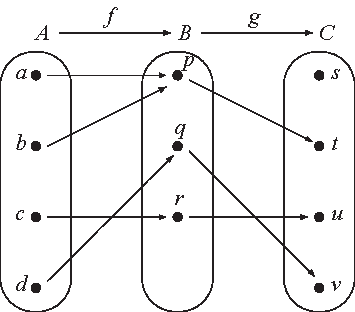
\includegraphics[width=\linewidth]{external/figps-sec641.pdf}
\end{image}%
\tcblower
\end{figureptx}%
If we follow the arrows from the set \(A\) to the set \(C\), we will use the outputs of \(f\) as inputs of \(g\), and get the arrow diagram from \(A\) to \(C\) shown in \hyperref[x:figure:fig_arrow64-2]{Figure~{\xreffont\ref{x:figure:fig_arrow64-2}}, p.\,\pageref{x:figure:fig_arrow64-2}}. This diagram represents the composition of \(f\) followed by \(g\).%
\begin{figureptx}{Arrow Diagram for \(g \circ f\x  A \to C\)}{x:figure:fig_arrow64-2}{}%
\begin{image}{0.3}{0.4}{0.3}%
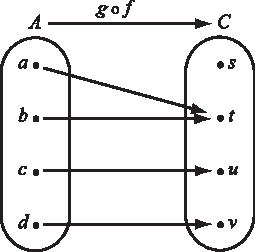
\includegraphics[width=\linewidth]{external/figps-sec642.pdf}
\end{image}%
\tcblower
\end{figureptx}%
\begin{inlineexercise}{The Composition of Two Functions.}{x:exercise:pr_compose}%
Let \(A = \{ a, b, c, d \}\) and \(B = \{ 1, 2, 3 \}\). Define the functions \(f\) and \(g\) as follows: \begin{quote}%
\(f \x A \to B\) defined by \(f(a) = 2\), \(f(b) = 3\), \(f(c) = 1\), and \(f(d) = 2\).\end{quote}
 \begin{quote}%
\(g \x B \to B\) defined by \(g(1) = 3\), \(g(2) = 1\), and \(g(3) = 2\).\end{quote}
%
\par
Create arrow diagrams for the functions \(f\), \(g\), \(g \circ f\), and \(g \circ g\).%
\space\hyperlink{g:solution:idm820517160-back}{[Solution]}\end{inlineexercise}%
\end{subsectionptx}
%
%
\typeout{************************************************}
\typeout{Subsection  Decomposing Functions}
\typeout{************************************************}
%
\begin{subsectionptx}{Decomposing Functions}{}{Decomposing Functions}{}{}{g:subsection:idm820510888}
\index{decomposing functions}%
\index{chain rule}%
We use the \terminology{chain rule} in calculus to find the derivative of a composite function. The first step in the process is to recognize a given function as a composite function. This can be done in many ways, but the work in \hyperref[x:worksheet:PA_verbaldescriptions]{Beginning Activity 2, p.\,\pageref{x:worksheet:PA_verbaldescriptions}} can be used to decompose a function in a way that works well with the chain rule. The use of the terms ``inner function'' and ``outer function'' can also be helpful. The idea is that we use the last step in the process to represent the outer function, and the steps prior to that to represent the inner function. So for the function,%
\begin{equation*}
f\x \mathbb{R} \to \mathbb{R}\text{  by  } f( x ) = ( {3x + 2} )^3\text{,}
\end{equation*}
the last step in the verbal description table was to cube the result. This means that we will use the function \(g\) (the cubing function) as the outer function and will use the prior steps as the inner function. We will denote the inner function by \(h\). So we let \(h\x \R \to \R\) by \(h( x ) = 3x + 2\) and \(g\x \R \to \R\) by \(g( x ) = x^3\). Then%
\begin{align*}
( {g \circ h} )( x ) \amp = g\left( {h( x )} \right)\\
\amp = g( {3x + 2} )\\
\amp = ( {3x + 2} )^3\\
\amp = f( x )\text{.}
\end{align*}
We see that \(g \circ h = f\) and, hence, we have ``decomposed'' the function \(f\). It should be noted that there are other ways to write the function \(f\) as a composition of two functions, but the way just described is the one that works well with the chain rule. In this case, the chain rule gives%
\begin{align*}
f'(x) \amp = ( g \circ h )'(x)\\
\amp = g'(h(x))\; h'(x)\\
\amp = 3(h(x))^2 \cdot 3\\
\amp = 9 (3x + 2)^2
\end{align*}
%
\begin{inlineexercise}{Decomposing Functions.}{x:exercise:prog_decompose}%
Write each of the following functions as the composition of two functions.%
\begin{enumerate}[font=\bfseries,label=(\alph*),ref=\alph*]
\item{}\(F\x \R \to \R\) by \(F(x) = ( x^2 +3 )^3\)%
\space\hyperlink{g:solution:idm820502696-back}{[Solution]}\item{}\(G\x \R \to \R\) by \(G(x) = \ln ( x^2 + 3 )\)%
\space\hyperlink{g:solution:idm820489256-back}{[Solution]}\item{}\(f\x \Z \to \Z\) by \(f(x) = | x^2 - 3 |\)%
\space\hyperlink{g:solution:idm820491560-back}{[Solution]}\item{}\(g\x \R \to \R\) by \(g(x) = \cos \! \left( \dfrac{2x-3}{x^2+1} \right)\)%
\space\hyperlink{g:solution:idm820488616-back}{[Solution]}\end{enumerate}
\end{inlineexercise}%
\end{subsectionptx}
%
%
\typeout{************************************************}
\typeout{Subsection  Theorems about Composite Functions}
\typeout{************************************************}
%
\begin{subsectionptx}{Theorems about Composite Functions}{}{Theorems about Composite Functions}{}{}{g:subsection:idm820487592}
If \(f \x A \to B\) and \(g \x B \to C\), then we can form the composite function \(g \circ f \x A \to C\). In \hyperref[x:section:S_typesoffunctions]{Section~{\xreffont\ref{x:section:S_typesoffunctions}}, p.\,\pageref{x:section:S_typesoffunctions}}, we learned about injections and surjections. We now explore what type of function \(g \circ f\) will be if the functions \(f\) and \(g\) are injections (or surjections).%
\begin{inlineexercise}{Compositions of Injections and Surjections.}{x:exercise:prog_compositesofinjections}%
Although other representations of functions can be used, it will be helpful to use arrow diagrams to represent the functions in this progress check. We will use the following sets:%
\begin{equation*}
A = \{ a, b, c \},  B = \{p, q, r\},  C = \{u, v, w, x \},  \text{ and }   D = \{u, v \}\text{.}
\end{equation*}
%
\begin{enumerate}[font=\bfseries,label=(\alph*),ref=\alph*]
\item{}Draw an arrow diagram for a function \(f \x A \to B\) that is an injection and an arrow diagram for a function \(g \x B \to C\) that is an injection. In this case, is the composite function \(g \circ f \x A \to C\) an injection? Explain.%
\space\hyperlink{g:solution:idm820479272-back}{[Solution]}\item{}Draw an arrow diagram for a function \(f \x A \to B\) that is a surjection and an arrow diagram for a function \(g \x B \to D\) that is a surjection. In this case, is the composite function \(g \circ f \x A \to D\) a surjection? Explain.%
\(g \circ f\) should be a surjection.%
\item{}Draw an arrow diagram for a function \(f \x A \to B\) that is a bijection and an arrow diagram for a function \(g \x B \to A\) that is a bijection. In this case, is the composite function \(g \circ f \x A \to A\) bijection? Explain.%
\space\hyperlink{g:solution:idm820471592-back}{[Solution]}\end{enumerate}
\end{inlineexercise}%
In \hyperref[x:exercise:prog_compositesofinjections]{Progress Check~{\xreffont\ref{x:exercise:prog_compositesofinjections}}, p.\,\pageref{x:exercise:prog_compositesofinjections}}, we explored some properties of composite functions related to injections, surjections, and bijections. The following theorem contains results that these explorations were intended to illustrate. Some of the proofs will be included in the exercises.%
\begin{theorem}{}{}{x:theorem:T_compositefunctions}%
Let \(A\), \(B\), and \(C\) be nonempty sets and assume that \(f\x A \to B\) and \(g\x B \to C\).%
\begin{enumerate}
\item\label{x:li:T_compositefunctions1}{}\hypertarget{x:li:T_compositefunctions1}{}If \(f\) and \(g\) are both injections, then \((g \circ f) \x A \to C\) is an injection.%
\item\label{x:li:T_compositefunctions2}{}\hypertarget{x:li:T_compositefunctions2}{}If \(f\) and \(g\) are both surjections, then \((g \circ f) \x A \to C\) is a surjection.%
\item\label{x:li:T_compositefunctions3}{}\hypertarget{x:li:T_compositefunctions3}{}If \(f\) and \(g\) are both bijections, then \((g \circ f) \x A \to C\) is a bijection.%
\end{enumerate}
%
\end{theorem}
The proof of \hyperlink{x:li:T_compositefunctions1}{Item~{\xreffont 1}, p.\,\pageref{x:li:T_compositefunctions1}} is \hyperlink{x:exercise:exer_compositefunctions1}{Exercise~{\xreffont 6}, p.\,\pageref{x:exercise:exer_compositefunctions1}}. \hyperlink{x:li:T_compositefunctions3}{Item~{\xreffont 3}, p.\,\pageref{x:li:T_compositefunctions3}} is a direct consequence of the first two parts. We will discuss a process for constructing a proof of \hyperlink{x:li:T_compositefunctions2}{Item~{\xreffont 2}, p.\,\pageref{x:li:T_compositefunctions2}}. Using the forward-backward process, we first look at the conclusion of the conditional statement in \hyperlink{x:li:T_compositefunctions2}{Item~{\xreffont 2}, p.\,\pageref{x:li:T_compositefunctions2}}. The goal is to prove that \(g \circ f\) is a surjection. Since \(g \circ f\x A \to C\), this is equivalent to proving that \begin{quote}%
For all \(c \in C\), there exists an \(a \in A\) such that \(( {g \circ f} )( a ) = c\).\end{quote}
 Since this statement in the backward process uses a universal quantifier, we will use the choose-an-element method and choose an arbitrary element \(c\) in the set \(C\). The goal now is to find an \(a \in A\) such that \(( {g \circ f} )( a ) = c\).%
\par
Now we can look at the hypotheses. In particular, we are assuming that both \(f\x A \to B\) and \(g\x B \to C\) are surjections. Since we have chosen \(c \in C\), and \(g\x B \to C\) is a surjection, we know that%
\begin{equation*}
\text{there exists a } b \in B \text{ such that } g( b ) = c\text{.}
\end{equation*}
Now, \(b \in B\) and \(f\x A \to B\) is a surjection. Hence%
\begin{equation*}
\text{there exists an } a \in A \text{ such that } f( a ) = b\text{.}
\end{equation*}
If we now compute \(( {g \circ f} )( a )\), we will see that%
\begin{equation*}
( {g \circ f} )( a ) = g \left( f ( a ) \right) = g ( b ) = c\text{.}
\end{equation*}
We can now write the proof as follows:%
\begin{paragraphs}{Proof of Theorem~{\xreffont\ref*{x:theorem:T_compositefunctions}}, Item~{\xreffont 2}.}{g:paragraphs:idm820451496}%
Let \(A\), \(B\), and \(C\) be nonempty sets and assume that \(f\x A \to B\) and \(g\x B \to C\) are both surjections. We will prove that \(g \circ f\x A \to C\) is a surjection.%
\par
Let \(c\) be an arbitrary element of \(C\). We will prove there exists an \(a \in A\) such that \(( g \circ f ) ( a ) = c\). Since \(g\x B \to C\) is a surjection, we conclude that%
\par
there exists a \(b \in B\) such that \(g( b ) = c\).%
\par
Now, \(b \in B\) and \(f\x A \to B\) is a surjection. Hence%
\begin{equation*}
\text{there exists an } a \in A \text{ such that } f( a ) = b\text{.}
\end{equation*}
We now see that%
\begin{align*}
( {g \circ f} )( a ) \amp = g\left( {f( a )} \right)\\
\amp = g( b )\\
\amp = c\text{.}
\end{align*}
%
\par
We have now shown that for every \(c \in C\), there exists an \(a \in A\) such that \(( {g \circ f} )( a ) = c\), and this proves that \(g \circ f\) is a surjection.%
\end{paragraphs}%
\par
\hyperref[x:theorem:T_compositefunctions]{Theorem~{\xreffont\ref{x:theorem:T_compositefunctions}}, p.\,\pageref{x:theorem:T_compositefunctions}} shows us that if \(f\) and \(g\) are both special types of functions, then the composition of \(f\) followed by \(g\) is also that type of function. The next question is, ``If the composition of \(f\) followed by \(g\) is an injection (or surjection), can we make any conclusions about \(f\) or \(g\)?'' A partial answer to this question is provided in \hyperref[x:theorem:T_morecompositefunctions]{Theorem~{\xreffont\ref{x:theorem:T_morecompositefunctions}}, p.\,\pageref{x:theorem:T_morecompositefunctions}}. This theorem will be investigated and proved in the Explorations and Activities for this section. See \hyperref[x:activity:exer_morecompositefunctions1]{Activity~{\xreffont\ref{x:activity:exer_morecompositefunctions1}}, p.\,\pageref{x:activity:exer_morecompositefunctions1}}.%
\begin{theorem}{}{}{x:theorem:T_morecompositefunctions}%
Let \(A\), \(B\), and \(C\) be nonempty sets and assume that \(f\x A \to B\) and \(g\x B \to C\).%
\begin{enumerate}
\item\label{x:li:T_morecompositefunctions1}{}\hypertarget{x:li:T_morecompositefunctions1}{}If \(g \circ f\x A \to C\) is an injection, then \(f\x A \to B\) is an injection.%
\item\label{x:li:T_morecompositefunctions2}{}\hypertarget{x:li:T_morecompositefunctions2}{}If \(g \circ f\x A \to C\) is a surjection, then \(g\x B \to C\) is a surjection.%
\end{enumerate}
%
\end{theorem}
\end{subsectionptx}
%
%
\typeout{************************************************}
\typeout{Exercises  Exercises}
\typeout{************************************************}
%
\begin{exercises-subsection}{Exercises}{}{Exercises}{}{}{g:exercises:idm820262312}
\begin{divisionexercise}{1}{}{}{x:exercise:exer_sec64-1}%
In our definition of the composition of two functions, \(f\) and \(g\), we required that the domain of \(g\) be equal to the codomain of \(f\). However, it is sometimes possible to form the composite function \(g \circ f\) even though \(\text{ dom} ( g ) \ne \text{ codom} ( f )\). For example, let%
\begin{align*}
\amp f: \R \to \R \amp \amp \text{ be defined by } \amp \amp f( x ) = x^2 + 1, \text{ and let}\\
\amp g: \R - \left\{ 0 \right\} \to \R \amp \amp \text{ be defined by } \amp \amp g( x ) = \dfrac{1}{x}
\end{align*}
%
\begin{enumerate}[font=\bfseries,label=(\alph*),ref=\alph*]
\item{}Is it possible to determine \(( {g \circ f} )( x )\) for all \(x \in \mathbb{R}\)? Explain.%
\item{}In general, let \(f\x A \to T\) and \(g\x B \to C\). Find a condition on the domain of \(g\) (other than \(B = T\)) that results in a meaningful definition of the composite function \(g \circ f\x A \to C\).%
\end{enumerate}
\end{divisionexercise}%
\begin{divisionexercise}{2}{}{}{x:exercise:exer64_notcommutative}%
Let \(h\x \mathbb{R} \to \mathbb{R}\) be defined by \(h( x ) = 3x + 2\) and \(g\x \mathbb{R} \to \mathbb{R}\) be defined by \(g( x ) = x^3\). Determine formulas for the composite functions \(g \circ h\) and \(h \circ g\). Is the function \(g \circ h\) equal to the function \(h \circ g\)? Explain. What does this tell you about the operation of composition of functions?%
\space\hyperlink{g:answer:idm820251048-back}{[Answer]}\end{divisionexercise}%
\begin{divisionexercise}{3}{}{}{x:exercise:exer_sec64-2}%
Following are formulas for certain real functions. Write each of these real functions as the composition of two functions. That is, decompose each of the functions.%
\begin{enumerate}[font=\bfseries,label=(\alph*),ref=\alph*]
\item{}\(F( x ) = \cos ( {e^x } )\)%
\space\hyperlink{g:answer:idm820242472-back}{[Answer]}\item{}\(G( x ) = e^{\cos ( x )}\)%
\space\hyperlink{g:answer:idm820245416-back}{[Answer]}\item{}\(H( x ) = \dfrac{1}{{\sin x}}\)%
\space\hyperlink{g:answer:idm820247976-back}{[Answer]}\item{}\(K( x ) = \cos \!\left( {e^{ - x^2 } } \right)\)%
\space\hyperlink{g:answer:idm820239784-back}{[Answer]}\end{enumerate}
\end{divisionexercise}%
\begin{divisionexercise}{4}{}{}{x:exercise:exer_sec64-4}%
\index{identity function}%
The \terminology{identity function} on a set \(S\), denoted by \(I_S\), is defined as follows: \(I_S \x S \to S\) by \(I_S ( x ) = x\) for each \(x \in S\). Let \(f\x A \to B\).%
\begin{enumerate}[font=\bfseries,label=(\alph*),ref=\alph*]
\item{}For each \(x \in A\), determine \(( {f \circ I_A } )( x )\) and use this to prove that \(f \circ I_A = f\).%
\space\hyperlink{g:answer:idm820229288-back}{[Answer]}\item{}Prove that \(I_B \circ f = f\).%
\end{enumerate}
\end{divisionexercise}%
\begin{divisionexercise}{5}{}{}{x:exercise:exer_sec64-3}%
Complete the following.%
\begin{enumerate}[font=\bfseries,label=(\alph*),ref=\alph*]
\item{}Let \(f\x \mathbb{R} \to \mathbb{R}\) be defined by \(f( x ) = x^2\), let \(g\x \mathbb{R} \to \mathbb{R}\) be defined by \(g( x ) = \sin x\), and let \(h\x \mathbb{R} \to \mathbb{R}\) be defined by \(h( x ) = \sqrt[3]{x}\).%
\par
Determine formulas for \(\left[ ( {h \circ g} ) \circ f \right] ( x )\) and \(\left[ h \circ ( {g \circ f} ) \right] ( x )\).%
\par
Does this prove that \(( {h \circ g} ) \circ f = h \circ ( {g \circ f} )\) for these particular functions? Explain.%
\space\hyperlink{g:answer:idm820228392-back}{[Answer]}\item{}Now let \(A\), \(B\), \(C\), and \(D\) be sets and let \(f\x A \to B\), \(g\x B \to C\), and \(h\x C \to D\). Prove that \(( {h \circ g} ) \circ f = h \circ ( {g \circ f} )\). That is, prove that function composition is an associative operation.%
\end{enumerate}
\end{divisionexercise}%
\begin{divisionexercise}{6}{}{}{x:exercise:exer_compositefunctions1}%
Prove \hyperlink{x:li:T_compositefunctions1}{Item~{\xreffont 1}, p.\,\pageref{x:li:T_compositefunctions1}} of \hyperref[x:theorem:T_compositefunctions]{Theorem~{\xreffont\ref{x:theorem:T_compositefunctions}}, p.\,\pageref{x:theorem:T_compositefunctions}}.%
\par
Let \(A\), \(B\), and \(C\) be nonempty sets and let \(f\x A \to B\) and \(g\x B \to C\). If \(f\) and \(g\) are both injections, then \(g \circ f\) is an injection.%
\space\hyperlink{g:answer:idm820212392-back}{[Answer]}\end{divisionexercise}%
\begin{divisionexercise}{7}{}{}{x:exercise:exer_sec64-8}%
For each of the following, give an example of functions \(f\x A \to B\) and \(g\x B \to C\) that satisfy the stated conditions, or explain why no such example exists.%
\begin{enumerate}[font=\bfseries,label=(\alph*),ref=\alph*]
\item{}The function \(f\) is a surjection, but the function \(g \circ f\) is not a surjection.%
\space\hyperlink{g:answer:idm820212520-back}{[Answer]}\item{}The function \(f\) is an injection, but the function \(g \circ f\) is not an injection.%
\space\hyperlink{g:answer:idm820207912-back}{[Answer]}\item{}The function \(g\) is a surjection, but the function \(g \circ f\) is not a surjection.%
\item{}The function \(g\) is an injection, but the function \(g \circ f\) is not an injection.%
\item{}The function \(f\) is not a surjection, but the function \(g \circ f\) is a surjection.%
\item{}The function \(f\) is not an injection, but the function \(g \circ f\) is an injection.%
\space\hyperlink{g:answer:idm820199720-back}{[Answer]}\item{}The function \(g\) is not a surjection, but the function \(g \circ f\) is a surjection.%
\item{}The function \(g\) is not an injection, but the function \(g \circ f\) is an injection.%
\end{enumerate}
\end{divisionexercise}%
\begin{divisionexercise}{8}{}{}{g:exercise:idm820194856}%
Let \(A\) be a nonempty set and let \(f\x A \to A\). For each \(n \in \N\), define a function \(f^n\x A \to A\) recursively as follows: \(f^1 = f\) and for each \(n \in \N\), \(f^{n+1} = f \circ f^n\). For example, \(f^2 = f \circ f^1 = f \circ f\) and \(f^3 = f \circ f^2 = f \circ ( f \circ f )\).%
\begin{enumerate}[font=\bfseries,label=(\alph*),ref=\alph*]
\item{}Let \(f\x \R \to \R\) by \(f(x) = x + 1\) for each \(x \in \R\). For each \(n \in \N\) and for each \(x \in \R\), determine a formula for \(f^n(x)\) and use induction to prove that your formula is correct.%
\item{}Let \(a, b \in \R\) and let \(f\x \R \to \R\) by \(f(x) = ax + b\) for each \(x \in \R\). For each \(n \in \N\) and for each \(x \in \R\), determine a formula for \(f^n(x)\) and use induction to prove that your formula is correct.%
\item{}Now let \(A\) be a nonempty set and let \(f\x A \to A\). Use induction to prove that for each \(n \in \N\), \(f^{n+1} = f^n \circ f\). (Note: You will need to use the result in \hyperlink{x:exercise:exer_sec64-3}{Exercise~{\xreffont 5}, p.\,\pageref{x:exercise:exer_sec64-3}}.)%
\end{enumerate}
\end{divisionexercise}%
\begin{activity}{Exploring Composite Functions.}{x:activity:exer_exploringcomposite}%
Let \(A\), \(B\), and \(C\) be nonempty sets and let \(f\x A \to B\) and \(g\x B \to C\). For this activity, it may be useful to draw your arrow diagrams in a triangular arrangement as follows:  \begin{image}{0.35}{0.3}{0.35}%
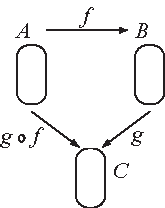
\includegraphics[width=\linewidth]{external/figps-comparrow.pdf}
\end{image}%
 It might be helpful to consider examples where the sets are small. Try constructing examples where the set \(A\) has 2 elements, the set \(B\) has 3 elements, and the set \(C\) has 2 elements.%
\begin{enumerate}[font=\bfseries,label=(\alph*),ref=\alph*]
\item{}Is it possible to construct an example where \(g \circ f\) is an injection, \(f\) is an injection, but \(g\) is not an injection? Either construct such an example or explain why it is not possible.%
\item{}Is it possible to construct an example where \(g \circ f\) is an injection, \(g\) is an injection, but \(f\) is not an injection? Either construct such an example or explain why it is not possible.%
\item{}Is it possible to construct an example where \(g \circ f\) is a surjection, \(f\) is a surjection, but \(g\) is not a surjection? Either construct such an example or explain why it is not possible.%
\item{}Is it possible to construct an example where \(g \circ f\) is surjection, \(g\) is a surjection, but \(f\) is not a surjection? Either construct such an example or explain why it is not possible.%
\end{enumerate}
\end{activity}%
\begin{activity}{The Proof of Theorem~{\xreffont\ref*{x:theorem:T_morecompositefunctions}}.}{x:activity:exer_morecompositefunctions1}%
Use the ideas from \hyperref[x:activity:exer_exploringcomposite]{Activity~{\xreffont\ref{x:activity:exer_exploringcomposite}}, p.\,\pageref{x:activity:exer_exploringcomposite}} to prove \hyperref[x:theorem:T_morecompositefunctions]{Theorem~{\xreffont\ref{x:theorem:T_morecompositefunctions}}, p.\,\pageref{x:theorem:T_morecompositefunctions}}. Let \(A\), \(B\), and \(C\) be nonempty sets and let \(f\x A \to B\) and \(g\x B \to C\).%
\begin{enumerate}[font=\bfseries,label=(\alph*),ref=\alph*]
\item\label{x:task:exer_sec64-6}If \(g \circ f\x A \to C\) is an injection, then \(f\x A \to B\) is an injection.%
\space\hyperlink{g:hint:idm820165544-back}{[Hint]}\par\smallskip%
\noindent\textbf{\blocktitlefont Hint}.\label{g:hint:idm820165544}{}\hypertarget{g:hint:idm820165544}{}\quad{}Start by asking, ``What do we have to do to prove that \(f\) is an injection?'' Start with a similar question for \hyperref[x:task:exer_sec64-7]{Task~{\xreffont\ref{x:activity:exer_morecompositefunctions1}}.{\xreffont\ref{x:task:exer_sec64-7}}, p.\,\pageref{x:task:exer_sec64-7}}.%
\item\label{x:task:exer_sec64-7}If \(g \circ f\x A \to C\) is a surjection, then \(g\x B \to C\) is a surjection.%
\end{enumerate}
\end{activity}%
\end{exercises-subsection}
\end{sectionptx}
%
%
\typeout{************************************************}
\typeout{Section 6.5 Inverse Functions}
\typeout{************************************************}
%
\begin{sectionptx}{Inverse Functions}{}{Inverse Functions}{}{}{x:section:S_inversefunctions}
\begin{introduction}{}%
For this section, we will use the concept of Cartesian product of two sets \(A\) and \(B\), denoted by \(A \times B\), which is the set of all ordered pairs \((x, y)\) where \(x \in A\) and \(y \in B\). That is, \(A \times B = \left\{ { {\left( {x,y} \right)} \mid x \in A\text{ and } y \in B} \right\}\). See \hyperref[x:worksheet:PA_cartesianproduct]{Beginning Activity 2, p.\,\pageref{x:worksheet:PA_cartesianproduct}} in \hyperref[x:section:S_cartesian]{Section~{\xreffont\ref{x:section:S_cartesian}}, p.\,\pageref{x:section:S_cartesian}} for a more thorough discussion of this concept.%
\end{introduction}%
%
%
\typeout{************************************************}
\typeout{Beginning Activity  Beginning Activity 1: Functions and Sets of Ordered Pairs}
\typeout{************************************************}
%
\begin{worksheet-subsection}{Beginning Activity 1: Functions and Sets of Ordered Pairs}{}{Beginning Activity 1: Functions and Sets of Ordered Pairs}{}{}{x:worksheet:PA_functionasordered}
When we graph a real function, we plot ordered pairs in the Cartesian plane where the first coordinate is the input of the function and the second coordinate is the output of the function. For example, if \(g\x \mathbb{R} \to \mathbb{R}\), then every point on the graph of \(g\) is an ordered pair \(( {x, y} )\) of real numbers where \(y = g( x )\). This shows how we can generate ordered pairs from a function. It happens that we can do this with any function. For example, let%
\begin{equation*}
A = \left\{ {1, 2, 3} \right\} \text{ and }  B = \left\{ {a, b} \right\}\text{.}
\end{equation*}
Define the function \(F\x A \to B\) by%
\begin{equation*}
F( 1 ) = a, F( 2 ) = b,  \text{ and } F( 3 ) = b\text{.}
\end{equation*}
%
\par
We can convert each of these to an ordered pair in \(A \times B\) by using the input as the first coordinate and the output as the second coordinate. For example, \(F( 1 ) = a\) is converted to \(( 1, a )\), \(F( 2 ) = b\) is converted to \(( 2, b )\), and \(F( 3 ) = b\) is converted to \(( 3, b )\). So we can think of this function as a set of ordered pairs, which is a subset of \(A \times B\), and write%
\begin{equation*}
F = \left\{ {( {1, a} ), ( {2, b} ), ( {3, b} )} \right\}\!\text{.}
\end{equation*}
%
\par
Note: Since \(F\) is the name of the function, it is customary to use \(F\) as the name for the set of ordered pairs.%
\begin{divisionexercise}{1}{}{}{g:exercise:idm820150184}%
Let \(A = \left\{ {1, 2, 3} \right\}\) and let \(C = \left\{ {a, b, c, d} \right\}\). Define the function \(g\x A \to C\) by \(g( 1 ) = a\), \(g( 2 ) = b\), and \(g( 3 ) = d\). Write the function \(g\) as a set of ordered pairs in \(A \times C\).%
\end{divisionexercise}%
For another example, if we have a real function, such as \(g\x \mathbb{R} \to \mathbb{R}\) by \(g( x ) = x^2  - 2\), then we can think of \(g\) as the following infinite subset of \(\mathbb{R} \times \mathbb{R}\):%
\begin{equation*}
g = \left\{ { {( {x, y} ) \in \mathbb{R} \times \mathbb{R}} \mid y = x^2  - 2} \right\}\!\text{.}
\end{equation*}
We can also write this as \(g = \left\{ {( {x, x^2 - 2} )} \mid x \in \mathbb{R} \right\}\).%
\begin{divisionexercise}{2}{}{}{g:exercise:idm820139688}%
Let \(f\x \Z \to \Z\) be defined by \(f(m) = 3m +5\), for all \(m \in \Z\). Use set builder notation to write the function \(f\) as a set of ordered pairs, and then use the roster method to write the function \(f\) as a set of ordered pairs.%
\end{divisionexercise}%
So any function \(f\x A \to B\) can be thought of as a set of ordered pairs that is a subset of \(A \times B\). This subset is%
\begin{equation*}
f = \left\{ { {( {a, f( a )} ) } \mid a \in A} \right\}  \text{ or } f = \left\{ {( {a, b} ) \in A \times B   \mid b = f( a )} \right\}\!\text{.}
\end{equation*}
On the other hand, if we started with \(A = \left\{ {1, 2, 3} \right\}\), \(B = \left\{ {a, b} \right\}\), and%
\begin{equation*}
G = \left\{ {( {1, a} ), ( {2, a} ), ( {3, b} )} \right\} \subseteq A \times B\text{,}
\end{equation*}
then we could think of \(G\) as a function from \(A\) to \(B\) with \(G( 1 ) = a\), \(G( 2 ) = a\), and \(G( 3 ) = b\). The idea is to use the first coordinate of each ordered pair as the input, and the second coordinate as the output. However, not every subset of \(A \times B\) can be used to define a function from \(A\) to \(B\). This is explored in the following questions.%
\begin{divisionexercise}{3}{}{}{g:exercise:idm820129960}%
Let \(f = \left\{ {( {1, a} ), ( {2, a} ), ( {3, a} ), ( {1, b} )} \right\}\). Could this set of ordered pairs be used to define a function from \(A\) to \(B\)? Explain.%
\end{divisionexercise}%
\begin{divisionexercise}{4}{}{}{g:exercise:idm820134568}%
Let \(g = \left\{ {( {1, a} ), ( {2, b} ), ( {3, a} )} \right\}\). Could this set of ordered pairs be used to define a function from \(A\) to \(B\)? Explain.%
\end{divisionexercise}%
\begin{divisionexercise}{5}{}{}{g:exercise:idm820131368}%
Let \(h = \left\{ {( {1, a} ), ( {2, b} )} \right\}\). Could this set of ordered pairs be used to define a function from \(A\) to \(B\)? Explain.%
\end{divisionexercise}%
\end{worksheet-subsection}
%
%
\typeout{************************************************}
\typeout{Beginning Activity  Beginning Activity 2: A Composition of Two Specific Functions}
\typeout{************************************************}
%
\begin{worksheet-subsection}{Beginning Activity 2: A Composition of Two Specific Functions}{}{Beginning Activity 2: A Composition of Two Specific Functions}{}{}{x:worksheet:PA_compositionoftwo}
Let \(A = \left\{ {a, b, c, d} \right\}\) and let \(B = \left\{ {p, q, r, s} \right\}\).%
\begin{divisionexercise}{1}{}{}{g:exercise:idm820125224}%
Construct an example of a function \(f\x A \to B\) that is a bijection. Draw an arrow diagram for this function.%
\end{divisionexercise}%
\begin{divisionexercise}{2}{}{}{x:exercise:PA_compositionoftwo2}%
On your arrow diagram, draw an arrow from each element of \(B\) back to its corresponding element in \(A\). Explain why this defines a function from \(B\) to \(A\).%
\end{divisionexercise}%
\begin{divisionexercise}{3}{}{}{g:exercise:idm820121512}%
If the name of the function in \hyperlink{x:exercise:PA_compositionoftwo2}{Exercise~{\xreffont 2}, p.\,\pageref{x:exercise:PA_compositionoftwo2}} is \(g\), so that \(g\x B \to A\), what are \(g( p )\), \(g( q )\), \(g( r )\), and \(g( s )\)?%
\end{divisionexercise}%
\begin{divisionexercise}{4}{}{}{x:exercise:PA_compositionoftwo4}%
Construct a table of values for each of the functions \(g \circ f\x A \to A\) and \(f \circ g\x B \to B\). What do you observe about these tables of values?%
\end{divisionexercise}%
\end{worksheet-subsection}
%
%
\typeout{************************************************}
\typeout{Subsection  The Ordered Pair Representation of a Function}
\typeout{************************************************}
%
\begin{subsectionptx}{The Ordered Pair Representation of a Function}{}{The Ordered Pair Representation of a Function}{}{}{g:subsection:idm820115112}
\index{function!as set of ordered pairs}%
In \hyperref[x:worksheet:PA_functionasordered]{Beginning Activity 1, p.\,\pageref{x:worksheet:PA_functionasordered}}, we observed that if we have a function \(f\x A \to B\), we can generate a set of ordered pairs \(f\) that is a subset of \(A \times B\) as follows:%
\begin{equation*}
f = \left\{ { {\left( {a, f( a )} \right)} \mid a \in A} \right\}  \text{ or } 
f = \left\{ {( {a, b} ) \in A \times B \mid b = f( a )} \right\}\!\text{.}
\end{equation*}
%
\par
However, we also learned that some sets of ordered pairs cannot be used to define a function. We now wish to explore under what conditions a set of ordered pairs can be used to define a function. Starting with a function \(f\x  A \to B\), since \(\text{ dom} ( f ) = A\), we know that%
\begin{equation}
\text{ For every }   a \in A, \text{ there exists a }   b \in B  \text{ such that } ( {a, b} ) 
\in f\text{.}\label{x:men:eq_65a}
\end{equation}
%
\par
Specifically, we use \(b = f( a )\). This says that every element of \(A\) can be used as an input. In addition, to be a function, each input can produce only one output. In terms of ordered pairs, this means that there will never be two ordered pairs \(( {a, b} )\) and \(( {a, c} )\) in the function \(f\) where \(a \in A\), \(b,
c \in B\), and \(b \ne c\). We can formulate this as a conditional statement as follows:%
\begin{align}
\amp \text{ For every }  a \in A \text{ and every }  b, c \in B, \amp \amp\notag\\
\amp \text{ if }  ( {a, b} ) \in f  \text{ and }  ( {a, c} ) 
\in f, \text{ then }  b = c\label{x:mrow:eq_65b}
\end{align}
%
\par
This also means that if we start with a subset \(f\) of \(A \times B\) that satisfies conditions \hyperref[x:men:eq_65a]{({\xreffont\ref{x:men:eq_65a}})} and \hyperref[x:mrow:eq_65b]{({\xreffont\ref{x:mrow:eq_65b}})}, then we can consider \(f\) to be a function from \(A\) to \(B\) by using \(b = f( a )\) whenever \(( {a, b} )\) is in \(f\). This proves the following theorem.%
\begin{theorem}{}{}{x:theorem:T_functionasordered}%
Let \(A\) and \(B\) be nonempty sets and let \(f\) be a subset of \(A \times B\) that satisfies the following two properties:%
\begin{itemize}[label=\textbullet]
\item{}For every \(a \in A\), there exists \(b \in B\) such that \(( {a, b} ) \in f\); and%
\item{}For every \(a \in A\) and every \(b, c \in B\), if \(( {a,\;b} ) \in f\) and \(( {a, c} ) \in f\), then \(b = c\).%
\end{itemize}
%
\par
If we use \(f( a ) = b\) whenever \(( {a, b} ) \in f\), then \(f\) is a function from \(A\) to \(B\).%
\end{theorem}
A Note about \hyperref[x:theorem:T_functionasordered]{Theorem~{\xreffont\ref{x:theorem:T_functionasordered}}, p.\,\pageref{x:theorem:T_functionasordered}}. The first condition in \hyperref[x:theorem:T_functionasordered]{Theorem~{\xreffont\ref{x:theorem:T_functionasordered}}, p.\,\pageref{x:theorem:T_functionasordered}} means that every element of \(A\) is an input, and the second condition ensures that every input has exactly one output. Many texts will use \hyperref[x:theorem:T_functionasordered]{Theorem~{\xreffont\ref{x:theorem:T_functionasordered}}, p.\,\pageref{x:theorem:T_functionasordered}} as the definition of a function. Many mathematicians believe that this ordered pair representation of a function is the most rigorous definition of a function. It allows us to use set theory to work with and compare functions. For example, equality of functions becomes a question of equality of sets. Therefore, many textbooks will use the ordered pair representation of a function as the definition of a function.%
\begin{inlineexercise}{Sets of Ordered Pairs that Are Not Functions.}{x:exercise:prog_ordered}%
Let \(A = \left\{ {1, 2, 3} \right\}\) and let \(B = \left\{ {a, b} \right\}\). Explain why each of the following subsets of \(A \times B\) cannot be used to define a function from \(A\) to \(B\).%
\begin{enumerate}[font=\bfseries,label=(\alph*),ref=\alph*]
\item{}\(F = \left\{ {( {1, a} ), ( {2, a} )} \right\}\).%
\space\hyperlink{g:solution:idm820089896-back}{[Solution]}\item{}\(G = \left\{ {( {1, a} ), ( {2, b} ), ( {3, c} ), ( {2, c} )} \right\}\).%
\space\hyperlink{g:solution:idm820090408-back}{[Solution]}\end{enumerate}
\end{inlineexercise}%
\end{subsectionptx}
%
%
\typeout{************************************************}
\typeout{Subsection  The Inverse of a Function}
\typeout{************************************************}
%
\begin{subsectionptx}{The Inverse of a Function}{}{The Inverse of a Function}{}{}{g:subsection:idm820088872}
In previous mathematics courses, we learned that the exponential function (with base \(e\)) and the natural logarithm function are inverses of each other. This was often expressed as follows:%
\begin{align*}
\amp \text{ For each }  x \in \R \text{ with }  x > 0 \text{ and for each }  y \in \R,\\
\amp y = \ln x \text{ if and only if }  x = e^y\text{.}
\end{align*}
%
\par
Notice that this means that \(x\) is the input and \(y\) is the output for the natural logarithm function if and only if \(y\) is the input and \(x\) is the output for the exponential function. In essence, the inverse function (in this case, the exponential function) reverses the action of the original function (in this case, the natural logarithm function). In terms of ordered pairs (input-output pairs), this means that if \(( {x, y} )\) is an ordered pair for a function, then \(( {y, x} )\) is an ordered pair for its inverse. This idea of reversing the roles of the first and second coordinates is the basis for our definition of the inverse of a function.%
\begin{assemblage}{Definition.}{x:assemblage:inversefunction}%
\label{g:notation:idm820084904} Let \(f\x A \to B\) be a function. The \terminology{inverse of \(\boldsymbol{f}\)}, denoted by \(f^{ - 1}\), is the set of ordered pairs \(\left\{ { {( {b, a} ) \in B \times A} \mid f( a ) = b} \right\}\). That is,%
\begin{equation*}
f^{ - 1}  = \left\{ { {( {b, a} ) \in B \times A} \mid f( a ) = b} \right\}\!\text{.}
\end{equation*}
%
\par
If we use the ordered pair representation for \(f\), we could also write%
\begin{equation*}
f^{ - 1}  = \left\{ { {( {b, a} ) \in B \times A} \mid ( {a, b} ) \in f} \right\}\!\text{.}
\end{equation*}
%
\end{assemblage}
Notice that this definition does not state that \(f^{ - 1}\) is a function. It is simply a subset of \(B \times A\). After we study the material in \hyperref[x:chapter:C_equivrelations]{Chapter~{\xreffont\ref{x:chapter:C_equivrelations}}, p.\,\pageref{x:chapter:C_equivrelations}}, we will say that this means that \(f^{ - 1}\) is a \terminology{relation} from \(B\) to \(A\). This fact, however, is not important to us now. We are mainly interested in the following question: \begin{assemblage}{}{g:assemblage:idm820070312}%
Under what conditions will the inverse of the function \(f\x A \to B\) be a function from \(B\) to \(A\)?%
\end{assemblage}
%
\begin{inlineexercise}{Exploring the Inverse of a Function.}{x:exercise:prog_exploringinverse}%
Let \(A = \left\{ {a, b, c} \right\}\), \(B = \left\{ {a,b,c,d} \right\}\), and \(C = \left\{ {p, q, r} \right\}\). Define%
\begin{center}%
{\tabularfont%
\begin{tabular}{lll}
\multicolumn{1}{lB}{\(f\x A \to C\) by}&\multicolumn{1}{lB}{\(g\x A \to C\) by}&\(h\x B \to C\) by\tabularnewline[0pt]
\multicolumn{1}{lB}{\(f( a ) = r\)}&\multicolumn{1}{lB}{\(g( a ) = p\)}&\(h( a ) = p\)\tabularnewline[0pt]
\multicolumn{1}{lB}{\(f( b ) = p\)}&\multicolumn{1}{lB}{\(g( b ) = q\)}&\(h( b ) = q\)\tabularnewline[0pt]
\multicolumn{1}{lB}{\(f( c ) = q\)}&\multicolumn{1}{lB}{\(g( c ) = p\)}&\(h( c ) = r\)\tabularnewline[0pt]
\multicolumn{1}{lB}{}&\multicolumn{1}{lB}{}&\(h( d ) = q\)
\end{tabular}
}%
\end{center}%
\begin{enumerate}[font=\bfseries,label=(\alph*),ref=\alph*]
\item\label{x:task:A_exploringinverse1}Draw an arrow diagram for each function.%
\item{}Determine the inverse of each function as a set of ordered pairs.%
\space\hyperlink{g:solution:idm820058536-back}{[Solution]}\item\label{x:task:A_exploringinverse3}Explain each of the following.%
\begin{enumerate}[font=\bfseries,label=(\roman*),ref=\theenumi.\roman*]
\item{}Is \(f^{ - 1}\) a function from \(C\) to \(A\)? Explain.%
\space\hyperlink{g:solution:idm820060712-back}{[Solution]}\item{}Is \(g^{ - 1}\) a function from \(C\) to \(A\)? Explain.%
\space\hyperlink{g:solution:idm820048552-back}{[Solution]}\item{}Is \(h^{ - 1}\) a function from \(C\) to \(B\)? Explain.%
\space\hyperlink{g:solution:idm820049320-back}{[Solution]}\end{enumerate}
\item{}Draw an arrow diagram for each inverse from \hyperref[x:task:A_exploringinverse3]{Task~{\xreffont\ref{x:exercise:prog_exploringinverse}}.{\xreffont\ref{x:task:A_exploringinverse3}}, p.\,\pageref{x:task:A_exploringinverse3}} that is a function. Use your existing arrow diagram from \hyperref[x:task:A_exploringinverse1]{Task~{\xreffont\ref{x:exercise:prog_exploringinverse}}.{\xreffont\ref{x:task:A_exploringinverse1}}, p.\,\pageref{x:task:A_exploringinverse1}} to draw this arrow diagram.%
\item{}Make a conjecture about what conditions on a function \(F\x S \to T\) will ensure that its inverse is a function from \(T\) to \(S\).%
\space\hyperlink{g:solution:idm820039080-back}{[Solution]}\end{enumerate}
\end{inlineexercise}%
We will now consider a general argument suggested by the explorations in \hyperref[x:exercise:prog_exploringinverse]{Progress Check~{\xreffont\ref{x:exercise:prog_exploringinverse}}, p.\,\pageref{x:exercise:prog_exploringinverse}}. By definition, if \(f\x A \to B\) is a function, then \(f^{ - 1}\) is a subset of \(B \times A\). However, \(f^{ - 1}\) may or may not be a function from \(B\) to \(A\). For example, suppose that \(s,
t \in A\) with \(s \ne t\) and \(f( s ) = f( t )\). This is represented in \hyperref[x:figure:fig_inversenotfunction]{Figure~{\xreffont\ref{x:figure:fig_inversenotfunction}}, p.\,\pageref{x:figure:fig_inversenotfunction}}.%
\begin{figureptx}{The Inverse Is Not a Function}{x:figure:fig_inversenotfunction}{}%
\begin{image}{0.3}{0.4}{0.3}%
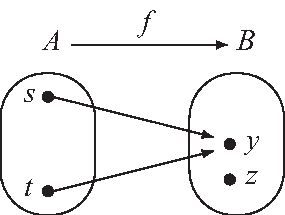
\includegraphics[width=\linewidth]{external/figps-noinverse.pdf}
\end{image}%
\tcblower
\end{figureptx}%
In this case, if we try to reverse the arrows, we will not get a function from \(B\) to \(A\). This is because \(( {y, s} ) \in f^{ - 1}\) and \(( {y, t} ) \in f^{ - 1}\) with \(s \ne t\). Consequently, \(f^{ - 1}\) is not a function. This suggests that when \(f\) is not an injection, then \(f^{ - 1}\) is not a function.%
\par
Also, if \(f\) is not a surjection, then there exists a \(z \in B\) such that \(f( a ) \ne z\) for all \(a \in A\), as in the diagram in \hyperref[x:figure:fig_inversenotfunction]{Figure~{\xreffont\ref{x:figure:fig_inversenotfunction}}, p.\,\pageref{x:figure:fig_inversenotfunction}}. In other words, there is no ordered pair in \(f\) with \(z\) as the second coordinate. This means that there would be no ordered pair in \(f^{ - 1}\) with \(z\) as a first coordinate. Consequently, \(f^{ - 1}\) cannot be a function from \(B\) to \(A\).%
\par
This motivates the statement in \hyperref[x:theorem:T_inverseandbijection]{Theorem~{\xreffont\ref{x:theorem:T_inverseandbijection}}, p.\,\pageref{x:theorem:T_inverseandbijection}}. In the proof of this theorem, we will frequently change back and forth from the input-output representation of a function and the ordered pair representation of a function. The idea is that if \(G\x S \to T\) is a function, then for \(s \in S\) and \(t \in T\),%
\begin{equation*}
G( s ) = t  \text{ if and only if }   ( {s, t} ) \in G\text{.}
\end{equation*}
%
\par
When we use the ordered pair representation of a function, we will also use the ordered pair representation of its inverse. In this case, we know that%
\begin{equation*}
( {s, t} ) \in G\text{ if and only if } ( {t, s} ) \in G^{ - 1}\text{.}
\end{equation*}
%
\begin{theorem}{}{}{x:theorem:T_inverseandbijection}%
Let \(A\) and \(B\) be nonempty sets and let \(f\x A \to B\). The inverse of \(f\) is a function from \(B\) to \(A\) if and only if \(f\) is a bijection.%
\end{theorem}
\begin{proof}{}{g:proof:idm820027560}
Let \(A\) and \(B\) be nonempty sets and let \(f\x A \to B\). We will first assume that \(f\) is a bijection and prove that \(f^{ - 1}\) is a function from \(B\) to \(A\). To do this, we will show that \(f^{ - 1}\) satisfies the two conditions of \hyperref[x:theorem:T_functionasordered]{Theorem~{\xreffont\ref{x:theorem:T_functionasordered}}, p.\,\pageref{x:theorem:T_functionasordered}}.%
\par
We first choose \(b \in B\). Since the function \(f\) is a surjection, there exists an \(a \in A\) such that \(f( a ) = b\). This implies that \(( {a, b} ) \in f\) and hence that \(( {b, a} ) \in f^{ - 1}\). Thus, each element of \(B\) is the first coordinate of an ordered pair in \(f^{ - 1}\), and hence \(f^{ - 1}\) satisfies the first condition of \hyperref[x:theorem:T_functionasordered]{Theorem~{\xreffont\ref{x:theorem:T_functionasordered}}, p.\,\pageref{x:theorem:T_functionasordered}}.%
\par
To prove that \(f^{ - 1}\) satisfies the second condition of \hyperref[x:theorem:T_functionasordered]{Theorem~{\xreffont\ref{x:theorem:T_functionasordered}}, p.\,\pageref{x:theorem:T_functionasordered}}, we must show that each element of \(B\) is the first coordinate of exactly one ordered pair in \(f^{ - 1}\). So let \(b \in B\), \(a_1 , a_2  \in A\) and assume that%
\begin{equation*}
( {b, a_1 } ) \in f^{ - 1} \text{ and }  ( {b, a_2 } ) \in f^{ - 1}\text{.}
\end{equation*}
This means that \(( {a_1 , b} ) \in f\) and \(( {a_2 , b} ) \in f\). We can then conclude that%
\begin{equation*}
f( {a_1 } ) = b\text{ and } f( {a_2 } ) = b\text{.}
\end{equation*}
But this means that \(f( {a_1 } ) = f( {a_2 } )\). Since \(f\) is a bijection, it is an injection, and we can conclude that \(a_1 = a_2\). This proves that \(b\) is the first element of only one ordered pair in \(f^{ - 1}\). Consequently, we have proved that \(f^{ - 1}\) satisfies both conditions of \hyperref[x:theorem:T_functionasordered]{Theorem~{\xreffont\ref{x:theorem:T_functionasordered}}, p.\,\pageref{x:theorem:T_functionasordered}} and hence that \(f^{ - 1}\) is a function from \(B\) to \(A\).%
\par
We now assume that \(f^{ - 1}\) is a function from \(B\) to \(A\) and prove that \(f\) is a bijection. First, to prove that \(f\) is an injection, we assume that \(a_1 , a_2  \in A\) and that \(f( {a_1 } ) = f( {a_2 } )\). We wish to show that \(a_1  = a_2\). If we let \(b = f( {a_1 } ) = f( {a_2 } )\), we can conclude that%
\begin{equation*}
( {a_1 , b} ) \in f \text{ and } ( {a_2 , b} ) \in f\text{.}
\end{equation*}
But this means that%
\begin{equation*}
( {b, a_1 } ) \in f^{ - 1} \text{ and } ( {b, a_2 } ) \in f^{ - 1}\text{.}
\end{equation*}
Since we have assumed that \(f^{ - 1}\) is a function, we can conclude that \(a_1 = a_2\). Hence, \(f\) is an injection.%
\par
Now to prove that \(f\) is a surjection, we choose \(b \in B\) and will show that there exists an \(a \in A\) such that \(f( a ) = b\). Since \(f^{ - 1}\) is a function, \(b\) must be the first coordinate of some ordered pair in \(f^{ - 1}\). Consequently, there exists an \(a \in A\) such that%
\begin{equation*}
( {b, a} ) \in f^{ - 1}\text{.}
\end{equation*}
Now this implies that \(( {a, b} ) \in f\) and hence that \(f( a ) = b\). This proves that \(f\) is a surjection. Since we have also proved that \(f\) is an injection, we conclude that \(f\) is a bijection.%
\end{proof}
\end{subsectionptx}
%
%
\typeout{************************************************}
\typeout{Subsection  Inverse Function Notation}
\typeout{************************************************}
%
\begin{subsectionptx}{Inverse Function Notation}{}{Inverse Function Notation}{}{}{g:subsection:idm820000024}
\index{invertible function}\index{function!invertible} In the situation where \(f\x A \to B\) is a bijection and \(f^{ - 1}\) is a function from \(B\) to \(A\), we can write \(f^{ - 1} \x B \to A\). In this case, we frequently say that \(f\) is an \terminology{invertible function}, and we usually do not use the ordered pair representation for either \(f\) or \(f^{ - 1}\). Instead of writing \(( {a, b} ) \in f\), we write \(f( a ) = b\), and instead of writing \(( {b, a} ) \in f^{ - 1}\), we write \(f^{ - 1} ( b ) = a\). Using the fact that \(( {a, b} ) \in f\) if and only if \(( {b, a} ) \in f^{ - 1}\), we can now write \(f( a ) = b\) if and only if \(f^{ - 1} ( b ) = a\). We summarize this in \hyperref[x:theorem:T_inversenotation]{Theorem~{\xreffont\ref{x:theorem:T_inversenotation}}, p.\,\pageref{x:theorem:T_inversenotation}}.%
\begin{theorem}{}{}{x:theorem:T_inversenotation}%
Let \(A\) and \(B\) be nonempty sets and let \(f\x A \to B\) be a bijection. Then \(f^{ - 1} \x B \to A\) is a function, and for every \(a \in A\) and \(b \in B\),%
\begin{equation*}
f( a ) = b  \text{ if and only if }  f^{ - 1} ( b ) = a\text{.}
\end{equation*}
%
\end{theorem}
\begin{example}{Inverse Function Notation.}{x:example:exam_inversenotation}%
For an example of the use of the notation in \hyperref[x:theorem:T_inversenotation]{Theorem~{\xreffont\ref{x:theorem:T_inversenotation}}, p.\,\pageref{x:theorem:T_inversenotation}}, let \(\R^ + = \left\{ { {x \in \R} \mid x > 0} \right\}\). Define%
\begin{equation*}
f\x \R \to \R \text{ by } f( x ) = x^3;
\text{ and } g\x \R \to \R^ + \text{ by }g( x ) = e^x\text{.}
\end{equation*}
Notice that \(\R^+\) is the codomain of \(g\). We can then say that both \(f\) and \(g\) are bijections. Consequently, the inverses of these functions are also functions. In fact, \(f^{ - 1} \x \R \to \R\) by \(f^{ - 1} ( y ) = \sqrt[3]{y}\); and \(g^{ - 1} \x \R^ + \to \R\) by \(g^{ - 1} ( y ) = \ln y\). For each function (and its inverse), we can write the result of \hyperref[x:theorem:T_inversenotation]{Theorem~{\xreffont\ref{x:theorem:T_inversenotation}}, p.\,\pageref{x:theorem:T_inversenotation}} as follows:%
\begin{center}%
{\tabularfont%
\begin{tabular}{ll}
\multicolumn{1}{lB}{\hyperref[x:theorem:T_inversenotation]{Theorem~{\xreffont\ref{x:theorem:T_inversenotation}}, p.\,\pageref{x:theorem:T_inversenotation}}}&Translates to:\tabularnewline\hrulemedium
\multicolumn{1}{lB}{\tablecelllines{l}{m}
{For  \(x, y \in \R\),  \(f( x ) = y\)\\
if and only if \(f^{ - 1} ( y ) = x\).}
}&\tablecelllines{l}{m}
{For \(x, y \in \R\),  \(x^3  = y\)\\
if and only if \(\sqrt[3]{y} = x\).}
\tabularnewline[0pt]
\multicolumn{1}{lB}{\tablecelllines{l}{m}
{For \(x \in \R, y \in \R^ +\),  \(g( x ) = y\)\\
if and only if  \(g^{ - 1} ( y ) = x\).}
}&\tablecelllines{l}{m}
{For \(x \in \R, y \in \R^ +\), \(e^x  = y\)\\
if and only if  \(\ln y = x\).}

\end{tabular}
}%
\end{center}%
\end{example}
\end{subsectionptx}
%
%
\typeout{************************************************}
\typeout{Subsection  Theorems about Inverse Functions}
\typeout{************************************************}
%
\begin{subsectionptx}{Theorems about Inverse Functions}{}{Theorems about Inverse Functions}{}{}{g:subsection:idm819976984}
The next two results in this section are two important theorems about inverse functions. The first is actually a corollary of \hyperref[x:theorem:T_inversenotation]{Theorem~{\xreffont\ref{x:theorem:T_inversenotation}}, p.\,\pageref{x:theorem:T_inversenotation}}.%
\begin{corollary}{}{}{x:corollary:C_inversecomposition}%
Let \(A\) and \(B\) be nonempty sets and let \(f\x A \to B\) be a bijection. Then%
\begin{enumerate}
\item\label{x:li:C_inversecomposition1}{}\hypertarget{x:li:C_inversecomposition1}{}For every \(x\) in \(A\), \(\left( f^{ - 1} \circ f \right)(x) = x\).%
\item\label{x:li:C_inversecomposition2}{}\hypertarget{x:li:C_inversecomposition2}{}For every \(y\) in \(B\), \(\left( f \circ f^{ - 1}\right)(y) = y\).%
\end{enumerate}
%
\end{corollary}
\begin{proof}{}{g:proof:idm819971480}
Let \(A\) and \(B\) be nonempty sets and assume that \(f\x A \to B\) is a bijection. So let \(x \in A\) and let \(f( x ) = y\). By \hyperref[x:theorem:T_inversenotation]{Theorem~{\xreffont\ref{x:theorem:T_inversenotation}}, p.\,\pageref{x:theorem:T_inversenotation}}, we can conclude that \(f^{ - 1} ( y ) = x\). Therefore,%
\begin{align*}
\left( {f^{ - 1}  \circ f} \right)( x ) \amp = f^{ - 1} \! \left( {f( x )} \right)\\
\amp = f^{-1}( y )\\
\amp = x\text{.}
\end{align*}
Hence, for each \(x \in A\), \(\left( {f^{ - 1} \circ f} \right)( x ) = x\).%
\par
The proof that for each \(y\) in \(B\), \(\left( f \circ f^{ - 1}\right)(y) = y\) is \hyperlink{x:exercise:exer_inversecomposition}{Exercise~{\xreffont 4}, p.\,\pageref{x:exercise:exer_inversecomposition}}.%
\end{proof}
\begin{example}{}{x:example:exam_inversenotation2}%
This example is a continuation of \hyperref[x:example:exam_inversenotation]{Example~{\xreffont\ref{x:example:exam_inversenotation}}, p.\,\pageref{x:example:exam_inversenotation}}.%
\par
For the cubing function and the cube root function, we have seen that For \(x, y \in \R\), \(x^3 = y\) if and only if \(\sqrt[3]{y} = x\). Notice that%
\begin{itemize}[label=\textbullet]
\item{}If we substitute \(x^3 = y\) into the equation \(\sqrt[3]{y} = x\), we obtain \(\sqrt[3]{{x^3 }} = x\).%
\item{}If we substitute \(\sqrt[3]{y} = x\) into the equation \(x^3 = y\), we obtain \(\left( {\sqrt[3]{y}} \right)^3 = y\).%
\end{itemize}
%
\par
This is an illustration of \hyperref[x:corollary:C_inversecomposition]{Corollary~{\xreffont\ref{x:corollary:C_inversecomposition}}, p.\,\pageref{x:corollary:C_inversecomposition}}. We can see this by using \(f\x \R \to \R\) defined by \(f( x ) = x^3\) and \(f^{ - 1} \x \R \to \R\) defined by \(f^{ - 1} ( y ) = \sqrt[3]{y}\). Then \(f^{ - 1}  \circ f\x \R \to \R\) and \(f^{ - 1}  \circ f = I_\R\). So for each \(x \in \R\),%
\begin{align*}
\left( {f^{ - 1}  \circ f} \right)( x ) \amp = x\\
f^{ - 1} \! \left( {f( x )} \right) \amp = x\\
f^{ - 1} \!\left( {x^3 } \right) \amp = x\\
\sqrt[3]{{x^3 }} \amp = x
\end{align*}
%
\par
Similarly, the equation \(\left( {\sqrt[3]{y}} \right)^3 = y\) for each \(y \in \R\) can be obtained from the fact that for each \(y \in \R\), \((f \circ f^{ - 1})(y) = y\).%
\end{example}
We will now consider the case where \(f\x A \to B\) and \(g\x B \to C\) are both bijections. In this case, \(f^{ - 1} \x B \to A\) and \(g^{ - 1} \x C \to B\). \hyperref[x:figure:fig_bijectioncomposition]{Figure~{\xreffont\ref{x:figure:fig_bijectioncomposition}}, p.\,\pageref{x:figure:fig_bijectioncomposition}} can be used to illustrate this situation.%
\begin{figureptx}{Composition of Two Bijections}{x:figure:fig_bijectioncomposition}{}%
\begin{image}{0.15}{0.7}{0.15}%
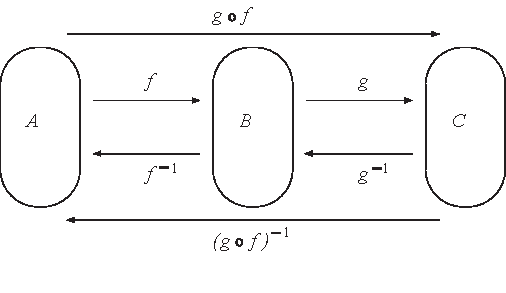
\includegraphics[width=\linewidth]{external/figps-compinverse.pdf}
\end{image}%
\tcblower
\end{figureptx}%
By \hyperref[x:theorem:T_compositefunctions]{Theorem~{\xreffont\ref{x:theorem:T_compositefunctions}}, p.\,\pageref{x:theorem:T_compositefunctions}}, \(g \circ f\x A \to C\) is also a bijection. Hence, by \hyperref[x:theorem:T_inverseandbijection]{Theorem~{\xreffont\ref{x:theorem:T_inverseandbijection}}, p.\,\pageref{x:theorem:T_inverseandbijection}}, \(( {g \circ f} )^{ - 1}\) is a function and, in fact, \(( {g \circ f} )^{ - 1} \x C \to A\). Notice that we can also form the composition of \(g^{ - 1}\) followed by \(f^{ - 1}\) to get \(f^{ - 1} \circ g^{ - 1} \x C \to A\). \hyperref[x:figure:fig_bijectioncomposition]{Figure~{\xreffont\ref{x:figure:fig_bijectioncomposition}}, p.\,\pageref{x:figure:fig_bijectioncomposition}} helps illustrate the result of the next theorem.%
\begin{theorem}{}{}{x:theorem:compositionofbijections}%
Let \(f\x A \to B\) and \(g\x B \to C\) be bijections. Then \(g \circ f\) is a bijection and \(( {g \circ f} )^{ - 1} = f^{ - 1} \circ g^{ - 1}\).%
\end{theorem}
\begin{proof}{}{g:proof:idm819931672}
Let \(f\x A \to B\) and \(g\x B \to C\) be bijections. Then \(f^{ - 1} \x B \to A\) and \(g^{ - 1} \x C \to B\). Hence, \(f^{ - 1} \circ g^{ - 1} \x C \to A\). Also, by \hyperref[x:theorem:T_compositefunctions]{Theorem~{\xreffont\ref{x:theorem:T_compositefunctions}}, p.\,\pageref{x:theorem:T_compositefunctions}}, \(g \circ f\x A \to C\) is a bijection, and hence \(( {g \circ f} )^{ - 1} \x C \to A\). We will now prove that for each \(z \in C\), \(( {g \circ f} )^{ - 1} ( z ) = ( {f^{ - 1} \circ g^{ - 1} } )( z )\).%
\par
Let \(z \in C\). Since the function \(g\) is a surjection, there exists a \(y \in B\) such that%
\begin{equation}
g( y ) = z\text{.}\label{x:men:eq_compofbij1}
\end{equation}
%
\par
Also, since \(f\) is a surjection, there exists an \(x \in A\) such that%
\begin{equation}
f( x ) = y\text{.}\label{x:men:eq_compofbij2}
\end{equation}
%
\par
Now these two equations can be written in terms of the respective inverse functions as%
\begin{align}
g^{ - 1} ( z ) \amp = y; \text{ and }\label{x:mrow:eq_compofbij3}\\
f^{ - 1} ( y ) \amp = x\label{x:mrow:eq_compofbij4}
\end{align}
%
\par
Using equation \hyperref[x:mrow:eq_compofbij3]{({\xreffont\ref{x:mrow:eq_compofbij3}})} and equation \hyperref[x:mrow:eq_compofbij4]{({\xreffont\ref{x:mrow:eq_compofbij4}})}, we see that%
\begin{align}
\left( {f^{ - 1}  \circ g^{ - 1} } \right)( z ) \amp 
= f^{ - 1} \left( {g^{ - 1} ( z )} \right)\notag\\
\amp = f^{ - 1} ( y )\notag\\
\amp = x\text{.}\label{x:mrow:eq_compofbij5}
\end{align}
%
\par
Using equation \hyperref[x:men:eq_compofbij1]{({\xreffont\ref{x:men:eq_compofbij1}})} and equation \hyperref[x:men:eq_compofbij2]{({\xreffont\ref{x:men:eq_compofbij2}})} again, we see that \(( {g \circ f} )( x ) = z\). However, in terms of the inverse function, this means that%
\begin{equation}
( {g \circ f} )^{ - 1} ( z ) = x\text{.}\label{x:men:eq_compofbij6}
\end{equation}
%
\par
Comparing equation \hyperref[x:mrow:eq_compofbij5]{({\xreffont\ref{x:mrow:eq_compofbij5}})} and equation \hyperref[x:men:eq_compofbij6]{({\xreffont\ref{x:men:eq_compofbij6}})}, we have shown that for all \(z \in C\),%
\par
\(( {g \circ f} )^{ - 1} ( z ) = ( {f^{ - 1} \circ g^{ - 1} } )( z )\). This proves that \(( {g \circ f} )^{ - 1} = f^{ - 1} \circ g^{ - 1}\).%
\end{proof}
\end{subsectionptx}
%
%
\typeout{************************************************}
\typeout{Exercises  Exercises}
\typeout{************************************************}
%
\begin{exercises-subsection}{Exercises}{}{Exercises}{}{}{g:exercises:idm819922456}
\begin{divisionexercise}{1}{}{}{x:exercise:exer_sec65-1}%
Let \(A = \left\{ {1, 2, 3} \right\}\) and \(B = \left\{ {a, b, c} \right\}\).%
\begin{enumerate}[font=\bfseries,label=(\alph*),ref=\alph*]
\item{}Construct an example of a function \(f\x A \to B\) that is not a bijection. Write the inverse of this function as a set of ordered pairs. Is the inverse of \(f\) a function? Explain. If so, draw an arrow diagram for \(f\) and \(f^{ - 1}\).%
\item{}Construct an example of a function \(g\x A \to B\) that is a bijection. Write the inverse of this function as a set of ordered pairs. Is the inverse of \(g\) a function? Explain. If so, draw an arrow diagram for \(g\) and \(g^{ - 1}\).%
\end{enumerate}
\end{divisionexercise}%
\begin{divisionexercise}{2}{}{}{x:exercise:exer_sec65-2}%
Let  \(S = \left\{ {a, b, c, d} \right\}\). Define  \(f\x S \to S\) by defining  \(f\)  to be the following set of ordered pairs.%
\begin{equation*}
f = \left\{ {( {a, c} ), ( {b, b} ), ( {c, d} ), ( {d, a} )} \right\}
\end{equation*}
%
\begin{enumerate}[font=\bfseries,label=(\alph*),ref=\alph*]
\item\label{x:task:exer_bijectiona}Draw an arrow diagram to represent the function \(f\). Is the function \(f\) a bijection?%
\item{}Write the inverse of \(f\) as a set of ordered pairs. Is \(f^{ - 1}\) a function? Explain.%
\space\hyperlink{g:answer:idm819910680-back}{[Answer]}\item{}Draw an arrow diagram for \(f^{ - 1}\) using the arrow diagram from \hyperref[x:task:exer_bijectiona]{Task~{\xreffont 2}.{\xreffont\ref{x:task:exer_bijectiona}}, p.\,\pageref{x:task:exer_bijectiona}}.%
\item{}Compute \(\left( {f^{ - 1} \circ f} \right)( x )\) and \(\left( {f \circ f^{ - 1} } \right)( x )\) for each \(x\) in \(S\). What theorem does this illustrate?%
\space\hyperlink{g:answer:idm819905560-back}{[Answer]}\end{enumerate}
\end{divisionexercise}%
\begin{divisionexercise}{3}{}{}{x:exercise:exer_solveequation}%
Inverse functions can be used to help solve certain equations. The idea is to use an inverse function to undo the function.%
\begin{enumerate}[font=\bfseries,label=(\alph*),ref=\alph*]
\item\label{x:task:exer_solveequationa}Since the cube root function and the cubing function are inverses of each other, we can often use the cube root function to help solve an equation involving a cube. For example, the main step in solving the equation%
\begin{equation*}
( {2t - 1} )^3  = 20
\end{equation*}
is to take the cube root of each side of the equation. This gives%
\begin{align*}
\sqrt[3]{{( {2t - 1} )^3 }} \amp = \sqrt[3]{{20}}\\
2t - 1 \amp = \sqrt[3]{{20}}\text{.}
\end{align*}
Explain how this step in solving the equation is a use of \hyperref[x:corollary:C_inversecomposition]{Corollary~{\xreffont\ref{x:corollary:C_inversecomposition}}, p.\,\pageref{x:corollary:C_inversecomposition}}.%
\space\hyperlink{g:answer:idm819898648-back}{[Answer]}\item\label{x:task:exer_solveequationb}A main step in solving the equation \(e^{2t - 1} = 20\) is to take the natural logarithm of both sides of this equation. Explain how this step is a use of \hyperref[x:corollary:C_inversecomposition]{Corollary~{\xreffont\ref{x:corollary:C_inversecomposition}}, p.\,\pageref{x:corollary:C_inversecomposition}}, and then solve the resulting equation to obtain a solution for \(t\) in terms of the natural logarithm function.%
\space\hyperlink{g:answer:idm819898392-back}{[Answer]}\item{}How are the methods of solving the equations in \hyperref[x:task:exer_solveequationa]{Task~{\xreffont 3}.{\xreffont\ref{x:task:exer_solveequationa}}, p.\,\pageref{x:task:exer_solveequationa}} and \hyperref[x:task:exer_solveequationb]{Task~{\xreffont 3}.{\xreffont\ref{x:task:exer_solveequationb}}, p.\,\pageref{x:task:exer_solveequationb}} similar?%
\space\hyperlink{g:answer:idm819895064-back}{[Answer]}\end{enumerate}
\end{divisionexercise}%
\begin{divisionexercise}{4}{}{}{x:exercise:exer_inversecomposition}%
Prove \hyperlink{x:li:C_inversecomposition2}{Item~{\xreffont 2}, p.\,\pageref{x:li:C_inversecomposition2}} of \hyperref[x:corollary:C_inversecomposition]{Corollary~{\xreffont\ref{x:corollary:C_inversecomposition}}, p.\,\pageref{x:corollary:C_inversecomposition}}. Let \(A\) and \(B\) be nonempty sets and let \(f\x A \to B\) be a bijection. Then for every \(y\) in \(B\), \(\left( f \circ f^{ - 1}\right)(y) = y\).%
\space\hyperlink{g:answer:idm819891864-back}{[Answer]}\end{divisionexercise}%
\begin{divisionexercise}{5}{}{}{x:exercise:sym_idfunc1}%
\index{identity function}%
In \hyperref[x:exercise:pr_equalfunc]{Progress Check~{\xreffont\ref{x:exercise:pr_equalfunc}}, p.\,\pageref{x:exercise:pr_equalfunc}}, we defined the identity function on a set. The \terminology{identity function on the set \(\boldsymbol{T}\)}, denoted by \(I_T\) , is the function \(I_T \x T \to T\) defined by \(I_T ( t ) = t\) for every \(t\) in \(T\). Explain how \hyperref[x:corollary:C_inversecomposition]{Corollary~{\xreffont\ref{x:corollary:C_inversecomposition}}, p.\,\pageref{x:corollary:C_inversecomposition}} can be stated using the concept of equality of functions and the identity functions on the sets \(A\) and \(B\).%
\end{divisionexercise}%
\begin{divisionexercise}{6}{}{}{x:exercise:exer_compequalidentity}%
Let \(f\x A \to B\) and \(g\x B \to A\). Let \(I_A\) and \(I_B\) be the identity functions on the sets \(A\) and \(B\), respectively. Prove each of the following:%
\begin{enumerate}[font=\bfseries,label=(\alph*),ref=\alph*]
\item{}If \(g \circ f = I_A\), then \(f\) is an injection.%
\space\hyperlink{g:answer:idm819878808-back}{[Answer]}\item{}If \(f \circ g = I_B\), then \(f\) is a surjection.%
\space\hyperlink{g:answer:idm819874840-back}{[Answer]}\item{}If \(g \circ f = I_A\) and \(f \circ g = I_B\), then \(f\) and \(g\) are bijections and \(g = f^{ - 1}\).%
\end{enumerate}
\end{divisionexercise}%
\begin{divisionexercise}{7}{}{}{x:exercise:exer_sec65-6}%
Justify your conclusions for the following.%
\begin{enumerate}[font=\bfseries,label=(\alph*),ref=\alph*]
\item{}Define \(f\x \mathbb{R} \to \mathbb{R}\) by \(f( x ) = e^{ - x^2 }\). Is the inverse of \(f\) a function?%
\space\hyperlink{g:answer:idm819868824-back}{[Answer]}\item{}Let \(\mathbb{R}^* = \left\{ { {x \in \mathbb{R} } \mid x \geq 0} \right\}\). Define \(g\x \mathbb{R}^* \to ( {0, 1} ]\) by \(g( x ) = e^{ - x^2 }\). Is the inverse of \(g\) a function?%
\space\hyperlink{g:answer:idm819864856-back}{[Answer]}\end{enumerate}
\end{divisionexercise}%
\begin{divisionexercise}{8}{}{}{x:exercise:exer_restrictdoma}%
Complete the following.%
\begin{enumerate}[font=\bfseries,label=(\alph*),ref=\alph*]
\item{}Let \(f\x \mathbb{R} \to \mathbb{R}\) be defined by \(f( x ) = x^2\). Explain why the inverse of \(f\) is not a function.%
\item\label{x:task:exer_restrictdomb}Let \(\R^* = \left \{ t \in \R \mid t \geq 0 \right\}\). Define \(g \x \R^* \to \R^*\) by \(g(x) = x^2\). Explain why this squaring function (with a restricted domain and codomain) is a bijection.%
\item{}Explain how to define the square root function as the inverse of the function in \hyperref[x:task:exer_restrictdomb]{Task~{\xreffont 8}.{\xreffont\ref{x:task:exer_restrictdomb}}, p.\,\pageref{x:task:exer_restrictdomb}}.%
\item{}True or false: \(\left( \sqrt{x} \right)^2 = x\) for all \(x \in \mathbb{R}\) such that \(x \geq 0\).%
\item{}True or false: \(\sqrt{x^2} = x\) for all \(x \in \mathbb{R}\).%
\end{enumerate}
\end{divisionexercise}%
\begin{divisionexercise}{9}{}{}{x:exercise:exer_finversebijection}%
Prove the following: \begin{quote}%
If \(f\x A \to B\) is a bijection, then \(f^{ - 1} \x B \to A\) is also a bijection.\end{quote}
%
\end{divisionexercise}%
\begin{divisionexercise}{10}{}{}{x:exercise:exer_sec65-9}%
For each natural number  \(k\), let  \(A_k\) be a set, and for each natural number  \(n\), let  \(f_n \x A_n  \to A_{n + 1}\). For example,  \(f_1 \x A_1  \to A_2\), \(f_2 \x A_2  \to A_3\), \(f_3 \x A_3  \to A_4\), and so on. Use mathematical induction to prove that for each natural number \(n\) with \(n \geq 2\), if  \(f_1 , f_2 ,  \ldots , f_n\) are all bijections, then \(f_n  \circ f_{n - 1}  \circ  \cdots  \circ f_2  \circ f_1\) is a bijection and%
\begin{equation*}
( {f_n  \circ f_{n - 1}  \circ  \cdots  \circ f_2  \circ f_1 } )^{ - 1}  = f_1^{ - 1}  
\circ f_2^{ - 1}  \circ  \cdots  \circ f_{n - 1}^{ - 1}  \circ f_n^{ - 1}\text{.}
\end{equation*}
%
\par
Note: This is an extension of \hyperref[x:theorem:compositionofbijections]{Theorem~{\xreffont\ref{x:theorem:compositionofbijections}}, p.\,\pageref{x:theorem:compositionofbijections}}. In fact, \hyperref[x:theorem:compositionofbijections]{Theorem~{\xreffont\ref{x:theorem:compositionofbijections}}, p.\,\pageref{x:theorem:compositionofbijections}} is the basis step of this proof for  \(n = 2\).%
\end{divisionexercise}%
\begin{divisionexercise}{11}{}{}{g:exercise:idm819848600}%
Complete the following.%
\begin{enumerate}[font=\bfseries,label=(\alph*),ref=\alph*]
\item{}Define \(f\x \R \to \R\) by \(f(x) = x^2 - 4\) for all \(x \in \R\). Explain why the inverse of the function \(f\) is not a function.%
\item{}Let \(\R^* = \left\{ x \in \R \mid x \geq 0 \right\}\) and let \(T = \left\{ y \in \R \mid y \geq -4 \right\}\). Define \(F\x \R^* \to T\) by \(F(x) = x^2 - 4\) for all \(x \in \R^*\). Explain why the inverse of the function \(F\) is a function and find a formula for \(F^{-1}(y)\), where \(y \in T\).%
\end{enumerate}
\end{divisionexercise}%
\begin{divisionexercise}{12}{}{}{g:exercise:idm819835288}%
Let \(R_5 = \left\{ 0, 1, 2, 3, 4 \right\}\).%
\begin{enumerate}[font=\bfseries,label=(\alph*),ref=\alph*]
\item{}Define \(f\x R_5 \to R_5\) by \(f(x) = x^2 + 4 \pmod 5\) for all \(x \in R_5\). Write the inverse of \(f\) as a set of ordered pairs and explain why \(f^{-1}\) is not a function.%
\item{}Define \(g\x R_5 \to R_5\) by \(g(x) = x^3 + 4 \pmod 5\) for all \(x \in R_5\). Write the inverse of \(g\) as a set of ordered pairs and explain why \(g^{-1}\) is a function.%
\item\label{x:task:exer_cuberootc}Is it possible to write a formula for \(g^{-1}(y)\), where \(y \in R_5\)? The answer to this question depends on whether or not it is possible to define a cube root of elements of \(R_5\). Recall that for a real number \(x\), we define the cube root of \(x\) to be the real number \(y\) such that \(y^3 = x\). That is,%
\begin{equation*}
y = \sqrt[3]{x} \text{ if and only if } y^3 = x\text{.}
\end{equation*}
Using this idea, is it possible to define the cube root of each number in \(R_5\)? If so, what are \(\sqrt[3]{0}\), \(\sqrt[3]{1}\), \(\sqrt[3]{2}\), \(\sqrt[3]{3}\), and \(\sqrt[3]{4}\)?%
\item{}Now answer the question posed at the beginning of \hyperref[x:task:exer_cuberootc]{Task~{\xreffont 12}.{\xreffont\ref{x:task:exer_cuberootc}}, p.\,\pageref{x:task:exer_cuberootc}} If possible, determine a formula for \(g^{-1}(y)\) where \(g^{-1}\x R_5 \to R_5\).%
\end{enumerate}
\end{divisionexercise}%
\begin{activity}{Constructing an Inverse Function.}{g:activity:idm819821848}%
If \(f\x A \to B\) is a bijection, then we know that its inverse is a function. If we are given a formula for the function \(f\), it may be desirable to determine a formula for the function \(f^{ - 1}\). This can sometimes be done, while at other times it is very difficult or even impossible. Let \(f\x \R \to \R\) be defined by \(f( x ) = 2x^3 - 7\). A graph of this function would suggest that this function is a bijection.%
\begin{enumerate}[font=\bfseries,label=(\alph*),ref=\alph*]
\item{}Prove that the function \(f\) is an injection and a surjection.%
\item\label{x:task:A_constructinverse2}Let \(y \in \R\). One way to prove that \(f\) is a surjection is to set \(y = f( x )\) and solve for \(x\). If this can be done, then we would know that there exists an \(x \in \R\) such that \(f(x) = y\). For the function \(f\), we are using \(x\) for the input and \(y\) for the output. By solving for \(x\) in terms of \(y\), we are attempting to write a formula where \(y\) is the input and \(x\) is the output. This formula represents the inverse function.%
\par
Solve the equation \(y = 2x^3 - 7\) for \(x\). Use this to write a formula for \(f^{ - 1} ( y )\), where \(f^{ - 1} \x \R \to \R\).%
\item{}Use the result of \hyperref[x:task:A_constructinverse2]{Task~{\xreffont\ref{g:activity:idm819821848}}.{\xreffont\ref{x:task:A_constructinverse2}}, p.\,\pageref{x:task:A_constructinverse2}} to verify that for each \(x \in \R\), \(f^{ - 1} \!\left( {f( x )} \right) = x\) and for each \(y \in \R\), \(f \!\left( {f^{ - 1} ( y )} \right) = y\).%
\item\label{x:task:exer_constructinversea}Now let \(\R^+ = \left\{ { {y \in \mathbb{R}} \mid y > 0} \right\}\). Define \(g \x \mathbb{R} \to \R^+\) by \(g( x ) = e^{2x - 1}\).%
\par
Set \(y = e^{2x - 1}\) and solve for \(x\) in terms of \(y\).%
\item{}Use your work in \hyperref[x:task:exer_constructinversea]{Task~{\xreffont\ref{g:activity:idm819821848}}.{\xreffont\ref{x:task:exer_constructinversea}}, p.\,\pageref{x:task:exer_constructinversea}} to define a function \(h\x \mathbb{R}^ + \to \mathbb{R}\).%
\item{}For each \(x \in \mathbb{R}\), determine \(( {h \circ g} )( x )\) and for each \(y \in \mathbb{R}^ +\), determine \(( {g \circ h} )( y )\).%
\item{}Use \hyperlink{x:exercise:exer_compequalidentity}{Exercise~{\xreffont 6}, p.\,\pageref{x:exercise:exer_compequalidentity}} to explain why \(h = g^{ - 1}\).%
\end{enumerate}
\end{activity}%
\begin{activity}{The Inverse Sine Function.}{x:activity:A_inversesine}%
We have seen that in order to obtain an inverse function, it is sometimes necessary to restrict the domain (or the codomain) of a function.%
\begin{enumerate}[font=\bfseries,label=(\alph*),ref=\alph*]
\item\label{x:task:A_inversesine1}Let \(f\x \R \to \R\) be defined by \(f( x ) = \sin x\). Explain why the inverse of the function \(f\) is not a function. (A graph may be helpful.)%
\item\label{x:task:A_inversesine2}Notice that if we use the ordered pair representation, then the sine function can be represented as%
\begin{equation*}
f  = \left\{ { {( {x, y} ) \in \R \times \R } \mid y = \sin x} \right\}\!\text{.}
\end{equation*}
If we denote the inverse of the sine function by  \(\sin ^{ - 1}\), then%
\begin{equation*}
f^{ - 1}  = \left\{ { {( {y, x} ) \in \R \times \R } \mid y = \sin x} \right\}\!\text{.}
\end{equation*}
\hyperref[x:task:A_inversesine1]{Task~{\xreffont\ref{x:activity:A_inversesine}}.{\xreffont\ref{x:task:A_inversesine1}}, p.\,\pageref{x:task:A_inversesine1}} proves that  \(f^{ - 1}\)  is not a function. However, in previous mathematics courses, we frequently used the ``inverse sine function.'' This is not really the inverse of the sine function as defined in \hyperref[x:task:A_inversesine1]{Task~{\xreffont\ref{x:activity:A_inversesine}}.{\xreffont\ref{x:task:A_inversesine1}}, p.\,\pageref{x:task:A_inversesine1}} but, rather, it is the inverse of the sine function \terminology{restricted to the domain} \(\left[ {-\dfrac{{\pi }}{2}, \dfrac{\pi }{2}} \right]\).%
\par
Explain why the function \(F\x \left[ {- \dfrac{{\pi }}{2}, \dfrac{\pi }{2}} \right] 
\to \left[ { - 1, 1} \right]\) defined by \(F( x ) = \sin x\) is a bijection.%
\item\label{x:task:inversesine}\index{inverse sine function}%
\index{arcsine function}%
\label{g:notation:idm819791896}%
The inverse of the function in \hyperref[x:task:A_inversesine2]{Task~{\xreffont\ref{x:activity:A_inversesine}}.{\xreffont\ref{x:task:A_inversesine2}}, p.\,\pageref{x:task:A_inversesine2}} is itself a function and is called the \terminology{inverse sine function} (or sometimes the \terminology{arcsine function}).%
\par
What is the domain of the inverse sine function? What are the range and codomain of the inverse sine function?%
\item\label{x:task:restrictedsine}\label{g:notation:idm819794200}%
Let us now use  \(F ( x ) = \text{ Sin }  ( x )\) to represent the restricted sine function in \hyperref[x:task:A_inversesine2]{Task~{\xreffont\ref{x:activity:A_inversesine}}.{\xreffont\ref{x:task:A_inversesine2}}, p.\,\pageref{x:task:A_inversesine2}}. Therefore, \(F^{-1} ( x ) = \text{ Sin } ^{ - 1} ( x )\) can be used to represent the inverse sine function.  Observe that%
\begin{equation*}
F\x \left[ -{\frac{{\pi }}{2}, \frac{\pi }{2}} \right] \to \left[ { - 1, 1} \right] 
\text{ and } F^{ - 1} \x \left[ { - 1, 1} \right] \to \left[ -{\frac{{\pi }}{2}, 
\frac{\pi } {2}} \right]\text{.}
\end{equation*}
%
\par
Using this notation, explain why \begin{quote}%
\(\text{ Sin } ^{ - 1} y = x \text{ if and only if } 
\left[ {y = \sin x\text{ and } -\dfrac{{\pi }}{2} \leq x \leq \dfrac{\pi } {2}} \right]\);\end{quote}
 \begin{quote}%
\(\text{ Sin } \!\left( \text{ Sin } ^{-1} ( y ) \right) = y\) for all \(y \in \left[ -1, 1 \right]\); and\end{quote}
 \begin{quote}%
\(\text{ Sin } ^{-1} \!\left( \text{ Sin } ( x ) \right) = x\) for all \(x \in \left[ - \dfrac{\pi}{2}, \dfrac{\pi}{2} \right]\).\end{quote}
%
\end{enumerate}
\end{activity}%
\end{exercises-subsection}
\end{sectionptx}
%
%
\typeout{************************************************}
\typeout{Section 6.6 Functions Acting on Sets}
\typeout{************************************************}
%
\begin{sectionptx}{Functions Acting on Sets}{}{Functions Acting on Sets}{}{}{x:section:S_functionsonsets}
%
%
\typeout{************************************************}
\typeout{Beginning Activity  Beginning Activity 1: Functions and Sets}
\typeout{************************************************}
%
\begin{worksheet-subsection}{Beginning Activity 1: Functions and Sets}{}{Beginning Activity 1: Functions and Sets}{}{}{x:worksheet:PA_functionsandsets}
Let \(S = \left\{ a, b, c, d \right\}\) and \(T = \left\{ s, t, u \right\}\). Define \(f\x S \to T\) by%
\begin{align*}
f(a) \amp = s \amp   f(b) \amp = t \amp   f(c) \amp = t \amp   f(d) \amp = s\text{.}
\end{align*}
%
\begin{divisionexercise}{1}{}{}{g:exercise:idm819779992}%
Let \(A = \left\{ a,c \right\}\) and \(B = \left\{ a, d \right\}\). Notice that \(A\) and \(B\) are subsets of \(S\). Use the roster method to specify the elements of the following two subsets of \(T\):%
\begin{enumerate}[font=\bfseries,label=(\alph*),ref=\alph*]
\item{}\(\left\{ f ( x ) \mid x \in A \right\}\)%
\item{}\(\left\{ f ( x ) \mid x \in B \right\}\)%
\end{enumerate}
\end{divisionexercise}%
\begin{divisionexercise}{2}{}{}{g:exercise:idm819782808}%
Let \(C = \left\{ s, t \right\}\) and \(D = \left\{ s, u \right\}\). Notice that \(C\) and \(D\) are subsets of \(T\). Use the roster method to specify the elements of the following two subsets of \(S\):%
\begin{enumerate}[font=\bfseries,label=(\alph*),ref=\alph*]
\item{}\(\left\{ x \in S \mid f ( x ) \in C \right\}\)%
\item{}\(\left\{ x \in S \mid f ( x ) \in D \right\}\)%
\end{enumerate}
\end{divisionexercise}%
Now let \(g\x \R \to \R\) be defined by \(g ( x ) = x^2\), for each \(x \in \mathbb{R}\).%
\begin{divisionexercise}{3}{}{}{g:exercise:idm819772952}%
Let \(A = \left\{ 1, 2, 3, -1 \right\}\). Use the roster method to specify the elements of the set \(\left\{ g ( x ) \mid x \in A \right\}\).%
\end{divisionexercise}%
\begin{divisionexercise}{4}{}{}{g:exercise:idm819770648}%
Use the roster method to specify the elements of each of the following sets:%
\begin{enumerate}[font=\bfseries,label=(\alph*),ref=\alph*]
\item{}\(\left\{ x \in \R \mid g( x ) = 1 \right\}\)%
\item{}\(\left\{ x \in \R \mid g( x ) = 9 \right\}\)%
\item{}\(\left\{ x \in \R \mid g( x ) = 15 \right\}\)%
\item{}\(\left\{ x \in \R \mid g( x ) = -1 \right\}\)%
\end{enumerate}
\end{divisionexercise}%
\begin{divisionexercise}{5}{}{}{g:exercise:idm819774232}%
Let \(B = \left\{ 1, 9, 15, -1 \right\}\). Use the roster method to specify the elements of the set \(\left\{ x \in \mathbb{R} \mid g ( x ) \in B \right\}\).%
\end{divisionexercise}%
\end{worksheet-subsection}
%
%
\typeout{************************************************}
\typeout{Beginning Activity  Beginning Activity 2: Functions and Intervals}
\typeout{************************************************}
%
\begin{worksheet-subsection}{Beginning Activity 2: Functions and Intervals}{}{Beginning Activity 2: Functions and Intervals}{}{}{x:worksheet:PA_functionsandint}
Let \(g\x \mathbb{R} \to \mathbb{R}\) be defined by \(g ( x ) = x^2\), for each \(x \in \mathbb{R}\).%
\begin{divisionexercise}{1}{}{}{g:exercise:idm819763352}%
We will first determine where \(g\) maps the closed interval \(\left[ 1, 2 \right]\). (Recall that \([1, 2] = \left\{ x \in \R \mid 1 \leq x \leq 2 \right\}\).) That is, we will describe, in simpler terms, the set \(\left\{ g ( x ) \mid x \in \left[ 1, 2 \right] \right\}\). This is the set of all images of the real numbers in the closed interval \(\left[ 1, 2 \right]\).%
\begin{enumerate}[font=\bfseries,label=(\alph*),ref=\alph*]
\item{}Draw a graph of the function \(g\) using \(-3 \leq x \leq 3\).%
\item{}On the graph, draw the vertical lines \(x = 1\) and \(x = 2\) from the \(x\)-axis to the graph. Label the points \(P \!\left(1, f ( 1 ) \right)\) and \(Q \!\left(2, f ( 2 ) \right)\) on the graph.%
\item{}Now draw horizontal lines from the points \(P\) and \(Q\) to the \(y\)-axis. Use this information from the graph to describe the set \(\left\{ g ( x ) \mid x \in \left[ 1, 2 \right] \right\}\) in simpler terms. Use interval notation or set builder notation.%
\end{enumerate}
\end{divisionexercise}%
\begin{divisionexercise}{2}{}{}{g:exercise:idm819752472}%
We will now determine all real numbers that \(g\) maps into the closed interval \(\left[ 1, 4 \right]\). That is, we will describe the set \(\left\{ x \in \mathbb{R} \mid g ( x ) \in 
\left[ 1, 4 \right] \right\}\) in simpler terms. This is the set of all preimages of the real numbers in the closed interval \(\left[ 1, 4 \right]\).%
\begin{enumerate}[font=\bfseries,label=(\alph*),ref=\alph*]
\item{}Draw a graph of the function \(g\) using \(-3 \leq x \leq 3\).%
\item\label{x:task:PA_functionsandintb}On the graph, draw the horizontal lines \(y = 1\) and \(y = 4\) from the \(y\)-axis to the graph. Label all points where these two lines intersect the graph.%
\item{}Now draw vertical lines from the points in \hyperref[x:task:PA_functionsandintb]{Task~{\xreffont 2}.{\xreffont\ref{x:task:PA_functionsandintb}}, p.\,\pageref{x:task:PA_functionsandintb}} to the \(x\)-axis, and then use the resulting information to describe the set \(\left\{ x \in \mathbb{R} \mid g ( x ) \in \left[ 1, 4 \right] \right\}\) in simpler terms. (You will need to describe this set as a union of two intervals. Use interval notation or set builder notation.)%
\end{enumerate}
\end{divisionexercise}%
\end{worksheet-subsection}
%
%
\typeout{************************************************}
\typeout{Subsection  Functions Acting on Sets}
\typeout{************************************************}
%
\begin{subsectionptx}{Functions Acting on Sets}{}{Functions Acting on Sets}{}{}{g:subsection:idm819744408}
In our study of functions, we have focused on how a function ``maps'' individual elements of its domain to the codomain. We also studied the preimage of an individual element in its codomain. For example, if \(f\x \mathbb{R} \to \mathbb{R}\) is defined by \(f ( x ) = x^2\), for each \(x \in \mathbb{R}\), then%
\begin{itemize}[label=\textbullet]
\item{}\(f ( 2 ) = 4\). We say that \(f\) maps 2 to 4 or that 4 is the image of 2 under the function \(f\).%
\item{}Since \(f ( x ) = 4\) implies that \(x = 2\) or \(x = -2\), we say that the preimages of 4 are 2 and \(-2\) or that the set of preimages of 4 is \(\left\{ -2, 2 \right\}\).%
\end{itemize}
%
\par
For a function \(f\x S \to T\), the next step is to consider subsets of \(S\) or \(T\) and what corresponds to them in the other set. We did this in the beginning activities. We will give some definitions and then revisit the examples in the beginning activities in light of these definitions. We will first consider the situation where \(A\) is a subset of \(S\) and consider the set of outputs whose inputs are from \(A\). This will be a subset of \(T\).%
\begin{assemblage}{Definition.}{x:assemblage:imageofA}%
\label{g:notation:idm819680408} Let \(f\x S \to T\). If \(A \subseteq S\), then the \terminology{image of \(\boldsymbol{A}\) under \(\boldsymbol{f}\)} is the set \(f ( A )\), where%
\begin{equation*}
f ( A ) = \left\{f ( x ) \mid x \in A \right\}\!\text{.}
\end{equation*}
%
\par
If there is no confusion as to which function is being used, we call \(f ( A )\) \terminology{the image of \(\boldsymbol{A}\)}.%
\end{assemblage}
We now consider the situation in which \(C\) is a subset of \(T\) and consider the subset of \(A\) consisting of all elements of \(T\) whose outputs are in \(C\).%
\begin{assemblage}{Definition.}{x:assemblage:inverseimage}%
\label{g:notation:idm819673624} Let \(f\x S \to T\). If \(C \subseteq T\), then the \terminology{preimage of \(\boldsymbol{C}\) under \(\boldsymbol{f}\)} is the set \(f^{-1} ( C )\), where%
\begin{equation*}
f^{-1} ( C ) = \left\{x \in S \mid f ( x ) \in C \right\}\text{.}
\end{equation*}
%
\par
If there is no confusion as to which function is being used, we call \(f^{-1} ( C )\) \terminology{the preimage of \(\boldsymbol{C}\)}. The preimage of the set \(C\) under \(f\) is also called the \terminology{inverse image of \(\boldsymbol{C}\) under \(\boldsymbol{f}\)}.%
\end{assemblage}
Notice that the set \(f^{-1} ( C )\) is defined whether or not \(f^{-1}\) is a function.%
\begin{inlineexercise}{Beginning Activity 1 Revisited.}{x:exercise:prog_functionsandsets}%
Let \(S = \left\{ a, b, c, d \right\}\) and \(T = \left\{ s, t, u \right\}\). Define \(f\x S \to T\) by%
\begin{align*}
f(a) \amp = s \amp   f(b) \amp = t \amp   f(c) \amp = t \amp   f(d) \amp = s\text{.}
\end{align*}
%
\par
Let \(A = \left\{ a, c \right\}, B = \left\{ a, d \right\}, C = \left\{ s, t \right\}, 
\text{ and } D = \left\{ s, u \right\}\).%
\par
Use your work in \hyperref[x:worksheet:PA_functionsandsets]{Beginning Activity 1, p.\,\pageref{x:worksheet:PA_functionsandsets}} to determine each of the following sets:%
\begin{enumerate}[font=\bfseries,label=(\alph*),ref=\alph*]
\item{}\(f ( A )\)%
\space\hyperlink{g:solution:idm819663128-back}{[Solution]}\item{}\(f ( B )\)%
\space\hyperlink{g:solution:idm819656984-back}{[Solution]}\item{}\(f^{-1} ( C )\)%
\space\hyperlink{g:solution:idm819654168-back}{[Solution]}\item{}\(f^{-1} ( D )\)%
\space\hyperlink{g:solution:idm819653144-back}{[Solution]}\end{enumerate}
\end{inlineexercise}%
\begin{example}{Images and Preimages of Sets.}{x:example:exam_imageandinverse}%
Let \(f\x \mathbb{R} \to \mathbb{R}\) be defined by \(f( x ) = x^2\), for each \(x \in \mathbb{R}\). The following results are based on the examples in \hyperref[x:worksheet:PA_functionsandsets]{Beginning Activity 1, p.\,\pageref{x:worksheet:PA_functionsandsets}} and \hyperref[x:worksheet:PA_functionsandint]{Beginning Activity 2, p.\,\pageref{x:worksheet:PA_functionsandint}}.%
\begin{itemize}[label=\textbullet]
\item{}Let \(A = \left\{ 1, 2, 3, -1 \right\}\). Then \(f ( A ) = \left\{ 1, 4, 9 \right\}\).%
\item{}Let \(B = \left\{ 1, 9, 15, -1 \right\}\). Then \(f^{-1} ( B ) = \left\{ -\sqrt{15}, -3, -1, 1, 3, \sqrt{15} \right\}\).%
\end{itemize}
%
\par
The graphs from \hyperref[x:worksheet:PA_functionsandint]{Beginning Activity 2, p.\,\pageref{x:worksheet:PA_functionsandint}} illustrate the following results:%
\begin{itemize}[label=\textbullet]
\item{}If \(T\) is the closed interval \(\left[ 1, 2 \right]\), then the image of the set \(T\) is%
\begin{align*}
f ( T ) \amp = \left\{ f ( x ) \mid x \in \left[ 1, 2 \right] \right\}\\
\amp = \left[ 1, 4 \right]\text{.}
\end{align*}
%
\item{}If \(C\) is the closed interval \(\left[ 1, 4 \right]\), then the preimage of the set \(C\) is%
\begin{equation*}
f^{-1} ( C ) = \left\{ x \in \mathbb{R} \mid f ( x ) \in \left[ 1, 4 \right] \right\} = \left[ -2, -1 \right] \cup \left[ 1, 2 \right]\text{.}
\end{equation*}
%
\end{itemize}
%
\end{example}
\end{subsectionptx}
%
%
\typeout{************************************************}
\typeout{Subsection  Set Operations and Functions Acting on Sets}
\typeout{************************************************}
%
\begin{subsectionptx}{Set Operations and Functions Acting on Sets}{}{Set Operations and Functions Acting on Sets}{}{}{g:subsection:idm819637400}
We will now consider the following situation: Let \(S\) and \(T\) be sets and let \(f\) be a function from \(S\) to \(T\). Also, let \(A\) and \(B\) be subsets of \(S\) and let \(C\) and \(D\) be subsets of \(T\). In the remainder of this section, we will consider the following situations and answer the questions posed in each case.%
\begin{itemize}[label=\textbullet]
\item{}The set \(A \cap B\) is a subset of \(S\) and so \(f ( A \cap B )\) is a subset of \(T\). In addition, \(f ( A )\) and \(f ( B )\) are subsets of \(T\). Hence, \(f ( A ) \cap f ( B )\) is a subset of \(T\).%
\par
Is there any relationship between \(f ( A \cap B )\) and \(f ( A ) \cap f ( B )\)?%
\item{}The set \(A \cup B\) is a subset of \(S\) and so \(f ( A \cup B )\) is a subset of \(T\). In addition, \(f ( A )\) and \(f ( B )\) are subsets of \(T\). Hence, \(f ( A ) \cup f ( B )\) is a subset of \(T\).%
\par
Is there any relationship between \(f ( A \cup B )\) and \(f ( A ) \cup f ( B )\)?%
\item{}The set \(C \cap D\) is a subset of \(T\) and so \(f^{-1} ( C \cap D )\) is a subset of \(S\). In addition, \(f^{-1} ( C )\) and \(f^{-1} ( D )\) are subsets of \(S\). Hence, \(f^{-1} ( C ) \cap f^{-1} ( D )\) is a subset of \(S\).%
\par
Is there any relationship between the sets \(f^{-1} ( C \cap D )\) and \(f^{-1} ( C ) \cap f^{-1} ( D )\)?%
\item{}The set \(C \cup D\) is a subset of \(T\) and so \(f^{-1} ( C \cup D )\) is a subset of \(S\). In addition, \(f^{-1} ( C )\) and \(f^{-1} ( D )\) are subsets of \(S\). Hence, \(f^{-1} ( C ) \cup f^{-1} ( D )\) is a subset of \(S\).%
\par
Is there any relationship between the sets \(f^{-1} ( C \cup D )\) and \(f^{-1} ( C ) \cup f^{-1} ( D )\)?%
\end{itemize}
%
\par
These and other questions will be explored in the next progress check.%
\begin{inlineexercise}{Set Operations and Functions Acting on Sets.}{x:exercise:prog_setsandfunctions}%
In \hyperref[x:section:S_moreaboutfunctions]{Section~{\xreffont\ref{x:section:S_moreaboutfunctions}}, p.\,\pageref{x:section:S_moreaboutfunctions}}, we introduced functions involving congruences. For example, if we let%
\begin{equation*}
R_8 = \left\{0, 1, 2, 3, 4, 5, 6, 7 \right\}\text{,}
\end{equation*}
then we can define \(f\x  R_8 \to R_8\) by \(f ( x ) = r\), where \(\left( x^2 + 2 \right) \equiv r \pmod 8\) and \(r \in R_8\). Moreover, we shortened this notation to%
\begin{equation*}
f ( x ) = \left( x^2 + 2 \right) \pmod 8\text{.}
\end{equation*}
%
\par
We will use the following subsets of \(\R_8\):%
\begin{equation*}
A = \left\{ 1, 2, 4 \right\} \qquad B = \left\{ 3, 4, 6 \right\} \qquad
C = \left\{ 1, 2, 3 \right\} \qquad D = \left\{ 3, 4, 5 \right\}\text{.}
\end{equation*}
%
\begin{enumerate}[font=\bfseries,label=(\alph*),ref=\alph*]
\item{}Verify that \(f ( 0 ) = 2\), \(f ( 1 ) = 3\), \(f ( 2 ) = 6\), and \(f ( 3 ) = 3\). Then determine \(f ( 4 )\), \(f ( 5 )\), \(f ( 6 )\), and \(f ( 7 )\).%
\space\hyperlink{g:solution:idm819611288-back}{[Solution]}\item{}Determine \(f (A )\), \(f (B )\), \(f^{-1} (C )\), and \(f^{-1} (D )\).%
\space\hyperlink{g:solution:idm819605016-back}{[Solution]}\item{}For each of the following, determine the two subsets of \(R_8\) and then determine if there is a relationship between the two sets. For example, \(A \cap B = \left\{ 4 \right\}\) and since \(f(4) = 2\), we see that \(f ( A \cap B ) = \left\{ 2 \right\}\).%
\begin{enumerate}[font=\bfseries,label=(\roman*),ref=\theenumi.\roman*]
\item{}\(f ( A \cap B )\) and \(f ( A ) \cap f ( B )\)%
\space\hyperlink{g:solution:idm819601304-back}{[Solution]}\item{}\(f ( A \cup B )\) and \(f ( A ) \cup f ( B )\)%
\space\hyperlink{g:solution:idm819596056-back}{[Solution]}\item{}\(f^{-1} ( C \cap D )\) and \(f^{-1} ( C ) \cap f^{-1} ( D )\)%
\space\hyperlink{g:solution:idm819589400-back}{[Solution]}\item{}\(f^{-1} ( C \cup D )\) and \(f^{-1} ( C ) \cup f^{-1} ( D )\)%
\space\hyperlink{g:solution:idm819591320-back}{[Solution]}\end{enumerate}
\item{}Notice that \(f ( A )\) is a subset of the codomain, \(R_8\). Consequently, \(f^{-1} \!\left( f ( A ) \right)\) is a subset of the domain, \(R_8\). Is there any relation between \(A\) and \(f^{-1} \!\left( f ( A ) \right)\) in this case?%
\space\hyperlink{g:solution:idm819593496-back}{[Solution]}\item{}Notice that \(f^{-1} ( C )\) is a subset of the domain, \(R_8\). Consequently, \(f \!\left( f^{-1} ( C ) \right)\) is a subset of the codomain, \(R_8\). Is there any relation between \(C\) and \(f \!\left( f^{-1} ( C ) \right)\) in this case?%
\space\hyperlink{g:solution:idm819584920-back}{[Solution]}\end{enumerate}
\end{inlineexercise}%
\begin{inlineexercise}{Set Operations and Functions Acting on Sets.}{x:exercise:exam_setsandfunctions2}%
Define \(f\x \mathbb{R} \to \mathbb{R}\) by \(f ( x ) = x^2 + 2\) for all \(x \in \mathbb{R}\). It will be helpful to use the graph shown in \hyperref[x:figure:fig_examplein91]{Figure~{\xreffont\ref{x:figure:fig_examplein91}}, p.\,\pageref{x:figure:fig_examplein91}}.%
\begin{figureptx}{Graph for \hyperref[x:exercise:exam_setsandfunctions2]{Progress Check~{\xreffont\ref{x:exercise:exam_setsandfunctions2}}, p.\,\pageref{x:exercise:exam_setsandfunctions2}}}{x:figure:fig_examplein91}{}%
\begin{image}{0.25}{0.5}{0.25}%
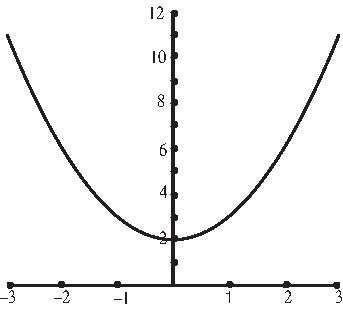
\includegraphics[width=\linewidth]{external/figps-setsandfunctions.pdf}
\end{image}%
Graph of a parabola opening up extending from x = -3 to x = 3 and y = 2 to y = 11.\tcblower
\end{figureptx}%
We will use the following closed intervals:%
\begin{equation*}
A = \left[ 0, 3 \right] \qquad B = \left[ -2, 1\right] \qquad
C = \left[ 2, 6 \right] \qquad D = \left[ 0, 3 \right]
\end{equation*}
%
\begin{enumerate}[font=\bfseries,label=(\alph*),ref=\alph*]
\item{}Verify that \(f ( A ) = [2, 11]\), \(f ( B ) = [2, 6]\), \(f^{-1} ( C ) = [-2, 2]\), and that \(f^{-1} ( D ) = [-1, 1]\).%
\item{}Explain why%
\begin{enumerate}[font=\bfseries,label=(\roman*),ref=\theenumi.\roman*]
\item{}\(f ( A \cap B ) = [2, 3]\) and \(f ( A ) \cap f ( B ) = [2, 6]\). So in this case, \(f ( A \cap B ) \subseteq f ( A ) \cap f ( B )\).%
\item{}\(f ( A \cup B ) = [2, 11]\) and \(f ( A ) \cup f ( B ) = [2, 11]\). So in this case, \(f ( A \cup B ) = f ( A ) \cup f ( B )\).%
\item{}\(f^{-1} ( C \cap D ) = [-1, 1]\) and \(f^{-1} ( C ) \cap f^{-1} ( D ) = [-1, 1]\). So in this case, \(f^{-1} ( C \cap D ) = f^{-1} ( C ) \cap f^{-1} ( D )\).%
\item{}\(f^{-1} ( C \cup D ) = [-2, 2]\) and \(f^{-1} ( C ) \cup f^{-1} ( D ) = [-2, 2]\). So in this case, \(f^{-1} ( C \cup D ) = f^{-1} ( C ) \cup f^{-1} ( D )\).%
\end{enumerate}
\item{}Recall that \(A = [0, 3]\). Notice \(f ( A ) = [2, 11]\) is a subset of the codomain, \(\mathbb{R}\). Explain why \(f^{-1} \!\left( f ( A ) \right) = [-3, 3]\). Since \(f^{-1} \!\left( f ( A ) \right)\) is a subset of the domain, \(\mathbb{R}\), we see that in this case, \(A \subseteq f^{-1} \!\left( f ( A ) \right)\).%
\item{}Recall that \(C = [2, 6]\). Notice that \(f^{-1} ( C ) = [-2, 2]\) is a subset of the domain, \(\mathbb{R}\). Explain why \(f \!\left( f^{-1} ( C ) \right) = [2, 6]\). Since \(f \!\left( f^{-1} ( C ) \right)\) is a subset of the codomain, \(\mathbb{R}\), we see that in this case \(f \!\left( f^{-1} ( C ) \right) = C\).%
\end{enumerate}
\end{inlineexercise}%
The examples in \hyperref[x:exercise:prog_setsandfunctions]{Progress Check~{\xreffont\ref{x:exercise:prog_setsandfunctions}}, p.\,\pageref{x:exercise:prog_setsandfunctions}} and \hyperref[x:exercise:exam_setsandfunctions2]{Progress Check~{\xreffont\ref{x:exercise:exam_setsandfunctions2}}, p.\,\pageref{x:exercise:exam_setsandfunctions2}} were meant to illustrate general results about how functions act on sets. In particular, we investigated how the action of a function on sets interacts with the set operations of intersection and union. We will now state the theorems that these examples were meant to illustrate. Some of the proofs will be left as exercises.%
\begin{theorem}{}{}{x:theorem:T_imageofoperations}%
Let \(f\x S \to T\) be a function and let \(A\) and \(B\) be subsets of \(S\). Then%
\begin{enumerate}
\item\label{x:li:T_imageofoperations1}{}\hypertarget{x:li:T_imageofoperations1}{}\index{image!of an intersection}\(\displaystyle f ( A \cap B ) \subseteq f ( A ) \cap f ( B )\)%
\item\label{x:li:T_imageofoperations2}{}\hypertarget{x:li:T_imageofoperations2}{}\index{image!of a union}\(\displaystyle f ( A \cup B ) = f ( A ) \cup f ( B )\)%
\end{enumerate}
%
\end{theorem}
\begin{proof}{}{g:proof:idm819558936}
We will prove \hyperlink{x:li:T_imageofoperations1}{Item~{\xreffont 1}, p.\,\pageref{x:li:T_imageofoperations1}}. The proof of \hyperlink{x:li:T_imageofoperations2}{Item~{\xreffont 2}, p.\,\pageref{x:li:T_imageofoperations2}} is \hyperlink{x:exercise:exer_sec91-5}{Exercise~{\xreffont 5}, p.\,\pageref{x:exercise:exer_sec91-5}}.%
\par
Assume that \(f\x S \to T\) is a function and let \(A\) and \(B\) be subsets of \(S\). We will prove that \(f ( A \cap B ) \subseteq f ( A ) \cap f ( B )\) by proving that for all \(y \in T\), if \(y \in f ( A \cap B )\), then \(y \in f ( A ) \cap f ( B )\).%
\par
We assume that \(y \in f ( A \cap B )\). This means that there exists an \(x \in A \cap B\) such that \(f ( x ) = y\). Since \(x \in A \cap B\), we conclude that \(x \in A\) and \(x \in B\).%
\begin{itemize}[label=\textbullet]
\item{}Since \(x \in A\) and \(f ( x ) = y\), we conclude that \(y \in f ( A )\).%
\item{}Since \(x \in B\) and \(f ( x ) = y\), we conclude that \(y \in f ( B )\).%
\end{itemize}
%
\par
Since \(y \in f ( A )\) and \(y \in f ( B )\), \(y \in f ( A ) \cap f ( B )\). This proves that if \(y \in f ( A \cap B )\), then \(y \in f ( A ) \cap f ( B )\). Hence \(f ( A \cap B ) \subseteq f ( A ) \cap f ( B )\).%
\end{proof}
\begin{theorem}{}{}{x:theorem:T_invimageofoperations}%
Let \(f\x S \to T\) be a function and let \(C\) and \(D\) be subsets of \(T\). Then%
\begin{enumerate}
\item\label{x:li:T_invimageofoperations1}{}\hypertarget{x:li:T_invimageofoperations1}{}\index{preimage!of an intersection}\(\displaystyle f^{-1} ( C \cap D ) = f^{-1} ( C ) \cap f^{-1} ( D )\)%
\item\label{x:li:T_invimageofoperations2}{}\hypertarget{x:li:T_invimageofoperations2}{}\index{preimage!of a union}\(\displaystyle f^{-1} ( C \cup D ) = f^{-1} ( C ) \cup f^{-1} ( D )\)%
\end{enumerate}
%
\end{theorem}
\begin{proof}{}{g:proof:idm819531416}
We will prove \hyperlink{x:li:T_invimageofoperations2}{Item~{\xreffont 2}, p.\,\pageref{x:li:T_invimageofoperations2}}. The proof of \hyperlink{x:li:T_invimageofoperations1}{Item~{\xreffont 1}, p.\,\pageref{x:li:T_invimageofoperations1}} is \hyperlink{x:exercise:exer_sec91-6}{Exercise~{\xreffont 6}, p.\,\pageref{x:exercise:exer_sec91-6}}.%
\par
Assume that \(f\x S \to T\) is a function and that \(C\) and \(D\) are subsets of \(T\). We will prove that \(f^{-1} ( C \cup D ) = f^{-1} ( C ) \cup f^{-1} ( D )\) by proving that each set is a subset of the other.%
\par
We start by letting \(x\) be an element of \(f^{-1} ( C \cup D )\). This means that \(f ( x )\) is an element of \(C \cup D\). Hence,%
\begin{equation*}
f ( x ) \in C \text{ or }  f ( x ) \in D\text{.}
\end{equation*}
In the case where \(f ( x ) \in C\), we conclude that \(x \in f^{-1} ( C )\), and hence that \(x \in f^{-1} ( C ) \cup f^{-1} ( D )\). In the case where \(f ( x ) \in D\), we see that \(x \in f^{-1} ( D )\), and hence that \(x \in f^{-1} ( C ) \cup f^{-1} ( D )\). So in both cases, \(x \in f^{-1} ( C ) \cup f^{-1} ( D )\), and we have proved that \(f^{-1} ( C \cup D ) \subseteq f^{-1} ( C ) \cup f^{-1} ( D )\).%
\par
We now let \(t \in f^{-1} ( C ) \cup f^{-1} ( D )\). This means that%
\begin{equation*}
t \in f^{-1} ( C ) \text{ or }  t \in f^{-1} ( D )\text{.}
\end{equation*}
%
\begin{itemize}[label=\textbullet]
\item{}In the case where \(t \in f^{-1} ( C )\), we conclude that \(f ( t ) \in C\) and hence that \(f ( t ) \in C \cup D\). This means that \(t \in f^{-1} ( C \cup D )\).%
\item{}Similarly, when \(t \in f^{-1} ( D )\), it follows that \(f ( t ) \in D\) and hence that \(f ( t ) \in C \cup D\). This means that \(t \in f^{-1} ( C \cup D )\).%
\end{itemize}
%
\par
These two cases prove that if \(t \in f^{-1} ( C ) \cup f^{-1} ( D )\), then \(t \in f^{-1} ( C \cup D )\). Therefore, \(f^{-1} ( C ) \cup f^{-1} ( D ) \subseteq f^{-1} ( C \cup D )\).%
\par
Since we have now proved that each of the two sets is a subset of the other set, we can conclude that \(f^{-1} ( C \cup D ) = f^{-1} ( C ) \cup f^{-1} ( D )\).%
\end{proof}
\begin{theorem}{}{}{x:theorem:T_imageofinvimage}%
Let \(f\x S \to T\) be a function and let \(A\) be a subset of \(S\) and let \(C\) be a subset of \(T\). Then%
\begin{multicols}{2}
\begin{enumerate}
\item\label{x:li:T_imageofinvimage1}{}\hypertarget{x:li:T_imageofinvimage1}{}\(\displaystyle A \subseteq f^{-1} \!\left( f ( A ) \right)\)%
\item\label{x:li:T_imageofinvimage2}{}\hypertarget{x:li:T_imageofinvimage2}{}\(\displaystyle f \!\left( f^{-1} ( C ) \right) \subseteq C\)%
\end{enumerate}
\end{multicols}
%
\end{theorem}
\begin{proof}{}{g:proof:idm819510040}
We will prove \hyperlink{x:li:T_imageofinvimage1}{Item~{\xreffont 1}, p.\,\pageref{x:li:T_imageofinvimage1}}. The proof of \hyperlink{x:li:T_imageofinvimage2}{Item~{\xreffont 2}, p.\,\pageref{x:li:T_imageofinvimage2}} is \hyperlink{x:exercise:exer_sec91-7}{Exercise~{\xreffont 7}, p.\,\pageref{x:exercise:exer_sec91-7}}.%
\par
To prove \hyperlink{x:li:T_imageofinvimage1}{Item~{\xreffont 1}, p.\,\pageref{x:li:T_imageofinvimage1}}, we will prove that for all \(a \in S\), if \(a \in A\), then%
\par
\(a \in f^{-1} \!\left( f ( A ) \right)\). So let \(a \in A\). Then, by definition, \(f ( a ) \in f ( A )\). We know that \(f ( A ) \subseteq T\), and so \(f^{-1} \!\left( f ( A ) \right) \subseteq S\). Notice that%
\begin{equation*}
f^{-1} \!\left( f ( A ) \right) = \left\{ x \in S \mid f ( x ) \in f ( A ) \right\}\text{.}
\end{equation*}
Since \(f ( a ) \in f ( A )\), we use this to conclude that \(a \in f^{-1}\!\left ( f ( A ) \right)\). This proves that if \(a \in A\), then \(a \in f^{-1} \!\left( f ( A ) \right)\), and hence that \(A \subseteq f^{-1} \!\left( f ( A ) \right)\).%
\end{proof}
\end{subsectionptx}
%
%
\typeout{************************************************}
\typeout{Exercises  Exercises}
\typeout{************************************************}
%
\begin{exercises-subsection}{Exercises}{}{Exercises}{}{}{g:exercises:idm819511192}
\begin{divisionexercise}{1}{}{}{x:exercise:exer_sec91-1}%
Let \(f\x S \to T\), let \(A\) and \(B\) be subsets of \(S\), and let \(C\) and \(D\) be subsets of \(T\). For \(x \in S\) and \(y \in T\), carefully explain what it means to say that%
\begin{enumerate}[font=\bfseries,label=(\alph*),ref=\alph*]
\item{}\(y \in f ( A \cap B )\)%
\space\hyperlink{g:answer:idm819496728-back}{[Answer]}\item{}\(y \in f ( A \cup B )\)%
\item{}\(y \in f ( A ) \cap f ( B )\)%
\item{}\(y \in f ( A ) \cup f ( B )\)%
\space\hyperlink{g:answer:idm819488536-back}{[Answer]}\item{}\(x \in f^{-1} ( C \cap D )\)%
\item{}\(x \in f^{-1} ( C \cup D )\)%
\space\hyperlink{g:answer:idm819491480-back}{[Answer]}\item{}\(x \in f^{-1} ( C ) \cap f^{-1} ( D )\)%
\item{}\(x \in f^{-1} ( C ) \cup f^{-1} ( D )\)%
\space\hyperlink{g:answer:idm819490328-back}{[Answer]}\end{enumerate}
\end{divisionexercise}%
\begin{divisionexercise}{2}{}{}{x:exercise:exer_sec91-2}%
Let \(f\x \mathbb{R} \to \mathbb{R}\) by \(f ( x ) = -2x + 1\). Let \(A = \left[ 2, 5 \right]\) \(B = \left[ -1, 3 \right]\) \(C = \left[ -2, 3 \right]\) \(D = \left[ 1, 4 \right]\). Find each of the following:%
\begin{enumerate}[font=\bfseries,label=(\alph*),ref=\alph*]
\item{}\(f ( A )\)%
\item{}\(f^{-1} ( f ( A ) )\)%
\space\hyperlink{g:answer:idm819481112-back}{[Answer]}\item{}\(f^{-1} ( C )\)%
\item{}\(f ( f^{-1} ( C ) )\)%
\space\hyperlink{g:answer:idm819482648-back}{[Answer]}\item{}\(f ( A \cap B )\)%
\space\hyperlink{g:answer:idm819478040-back}{[Answer]}\item{}\(f ( A ) \cap f ( B )\)%
\space\hyperlink{g:answer:idm819474968-back}{[Answer]}\item{}\(f^{-1} ( C \cap D )\)%
\item{}\(f^{-1} ( C ) \cap f^{-1} ( D )\)%
\end{enumerate}
\end{divisionexercise}%
\begin{divisionexercise}{3}{}{}{x:exercise:exer_sec91-3}%
Let \(g\x \mathbb{N} \times \mathbb{N} \to \mathbb{N}\) by \(g ( m, n ) = 2^m 3^n\), let \(A = \left\{ 1, 2, 3 \right\}\), and let \(C = \left\{ 1, 4, 6, 9, 12, 16, 18 \right\}\). Find%
\begin{enumerate}[font=\bfseries,label=(\alph*),ref=\alph*]
\item{}\(g ( A \times A )\)%
\space\hyperlink{g:answer:idm819479960-back}{[Answer]}\item{}\(g^{-1} ( C )\)%
\space\hyperlink{g:answer:idm819465752-back}{[Answer]}\item{}\(g^{-1} \!\left( g ( A \times A ) \right)\)%
\item{}\(g \!\left( g^{-1} ( C ) \right)\)%
\end{enumerate}
\end{divisionexercise}%
\begin{divisionexercise}{4}{}{}{x:exercise:exer_sec91-4}%
Let \(S = \left\{1, 2, 3, 4 \right\}\).%
\begin{enumerate}[font=\bfseries,label=(\alph*),ref=\alph*]
\item{}Define \(F\x S \to \mathbb{N}\) by \(F ( x ) = x^2\) for each \(x \in S\). What is the range of the function \(F\) and what is \(F ( S )\)? How do these two sets compare?%
\space\hyperlink{g:answer:idm819466392-back}{[Answer]}\item{}Now let \(A\) and \(B\) be sets and let \(f\x A \to B\) be an arbitrary function from \(A\) to \(B\).%
\par
Explain why \(f ( A ) = \text{ range} ( f )\).%
\item{}Define a function \(g\x A \to f ( A )\) by \(g ( x ) = f ( x )\) for all \(x\) in \(A\). Prove that the function \(g\) is a surjection.%
\end{enumerate}
\end{divisionexercise}%
\begin{divisionexercise}{5}{}{}{x:exercise:exer_sec91-5}%
Prove \hyperlink{x:li:T_imageofoperations2}{Item~{\xreffont 2}, p.\,\pageref{x:li:T_imageofoperations2}} of \hyperref[x:theorem:T_imageofoperations]{Theorem~{\xreffont\ref{x:theorem:T_imageofoperations}}, p.\,\pageref{x:theorem:T_imageofoperations}}. Let \(f\x S \to T\) be a function and let \(A\) and \(B\) be subsets of \(S\). Then \(f ( A \cup B ) = f ( A ) \cup f ( B )\).%
\space\hyperlink{g:answer:idm819456536-back}{[Answer]}\end{divisionexercise}%
\begin{divisionexercise}{6}{}{}{x:exercise:exer_sec91-6}%
Prove \hyperlink{x:li:T_invimageofoperations1}{Item~{\xreffont 1}, p.\,\pageref{x:li:T_invimageofoperations1}} of \hyperref[x:theorem:T_invimageofoperations]{Theorem~{\xreffont\ref{x:theorem:T_invimageofoperations}}, p.\,\pageref{x:theorem:T_invimageofoperations}}. Let \(f\x S \to T\) be a function and let \(C\) and \(D\) be subsets of \(T\). Then \(f^{-1} ( C \cap D ) = f^{-1} ( C ) \cap f^{-1} ( D )\).%
\space\hyperlink{g:answer:idm819445016-back}{[Answer]}\end{divisionexercise}%
\begin{divisionexercise}{7}{}{}{x:exercise:exer_sec91-7}%
Prove \hyperlink{x:li:T_imageofinvimage2}{Item~{\xreffont 2}, p.\,\pageref{x:li:T_imageofinvimage2}} of \hyperref[x:theorem:T_imageofinvimage]{Theorem~{\xreffont\ref{x:theorem:T_imageofinvimage}}, p.\,\pageref{x:theorem:T_imageofinvimage}}. Let \(f\x S \to T\) be a function and let \(C \subseteq T\). Then \(f \!\left( f^{-1} ( C ) \right) \subseteq C\).%
\end{divisionexercise}%
\begin{divisionexercise}{8}{}{}{g:exercise:idm819435288}%
Let \(f\x S \to T\) and let \(A\) and \(B\) be subsets of \(S\). Prove or disprove each of the following:%
\begin{enumerate}[font=\bfseries,label=(\alph*),ref=\alph*]
\item{}If \(A \subseteq B\), then \(f( A ) \subseteq f( B )\).%
\item{}If \(f ( A ) \subseteq f (B )\), then \(A \subseteq B\).%
\end{enumerate}
\end{divisionexercise}%
\begin{divisionexercise}{9}{}{}{x:exercise:exer_invimagetruefalse}%
Let \(f\x S \to T\) and let \(C\) and \(D\) be subsets of \(T\). Prove or disprove each of the following:%
\begin{enumerate}[font=\bfseries,label=(\alph*),ref=\alph*]
\item{}If \(C \subseteq D\), then \(f^{-1} ( C ) \subseteq f^{-1} (D )\).%
\space\hyperlink{g:answer:idm819427992-back}{[Answer]}\item{}If \(f^{-1} ( C ) \subseteq f^{-1} (D )\), then \(C \subseteq D\).%
\space\hyperlink{g:answer:idm819427480-back}{[Answer]}\end{enumerate}
\end{divisionexercise}%
\begin{divisionexercise}{10}{}{}{g:exercise:idm819430168}%
Prove or disprove:%
\par
If \(f\x S \to T\) is a function and \(A\) and \(B\) are subsets of \(S\), then \(f ( A ) \cap f ( B ) \subseteq f ( A \cap B )\).%
\par
Note: \hyperlink{x:li:T_imageofoperations1}{Item~{\xreffont 1}, p.\,\pageref{x:li:T_imageofoperations1}} of \hyperref[x:theorem:T_imageofoperations]{Theorem~{\xreffont\ref{x:theorem:T_imageofoperations}}, p.\,\pageref{x:theorem:T_imageofoperations}} states that \(f ( A \cap B ) \subseteq f ( A ) \cap f ( B )\).%
\end{divisionexercise}%
\begin{divisionexercise}{11}{}{}{x:exercise:exer_sec91-11}%
Let \(f\x S \to T\) be a function, let \(A \subseteq S\), and let \(C \subseteq T\).%
\begin{enumerate}[font=\bfseries,label=(\alph*),ref=\alph*]
\item{}\hyperlink{x:li:T_imageofinvimage1}{Item~{\xreffont 1}, p.\,\pageref{x:li:T_imageofinvimage1}} of \hyperref[x:theorem:T_imageofinvimage]{Theorem~{\xreffont\ref{x:theorem:T_imageofinvimage}}, p.\,\pageref{x:theorem:T_imageofinvimage}} states that \(A \subseteq f^{-1} \!\left( f ( A ) \right)\). Give an example where \(f^{-1} \!\left( f ( A ) \right) \not \subseteq A\).%
\item{}\hyperlink{x:li:T_imageofinvimage2}{Item~{\xreffont 2}, p.\,\pageref{x:li:T_imageofinvimage2}} of \hyperref[x:theorem:T_imageofinvimage]{Theorem~{\xreffont\ref{x:theorem:T_imageofinvimage}}, p.\,\pageref{x:theorem:T_imageofinvimage}} states that \(f \!\left( f^{-1} ( C ) \right) \subseteq C\). Give an example where \(C \not \subseteq f \!\left( f^{-1} ( C ) \right)\).%
\end{enumerate}
\end{divisionexercise}%
\begin{divisionexercise}{12}{}{}{x:exercise:exer_sec91-12}%
Is the following proposition true or false? Justify your conclusion with a proof or a counterexample. \begin{quote}%
If \(f\x S \to T\) is an injection and \(A \subseteq S\), then \(f^{-1} \!\left( f ( A ) \right) = A\).\end{quote}
%
\end{divisionexercise}%
\begin{divisionexercise}{13}{}{}{x:exercise:exer_sec91-13}%
Is the following proposition true or false? Justify your conclusion with a proof or a counterexample. \begin{quote}%
If \(f\x S \to T\) is a surjection and \(C \subseteq T\), then \(f \!\left( f^{-1} ( C ) \right) = C\).\end{quote}
%
\end{divisionexercise}%
\begin{divisionexercise}{14}{}{}{g:exercise:idm819410728}%
Let \(f\x S \to T\). Prove that \(f ( A \cap B ) = f ( A ) \cap f ( B )\) for all subsets \(A\) and \(B\) of \(S\) if and only if \(f\) is an injection.%
\end{divisionexercise}%
\end{exercises-subsection}
\end{sectionptx}
%
%
\typeout{************************************************}
\typeout{Section 6.7 Chapter~{\xreffont\ref*{x:chapter:C_functions}} Summary}
\typeout{************************************************}
%
\begin{sectionptx}{Chapter~{\xreffont\ref*{x:chapter:C_functions}} Summary}{}{Chapter~{\xreffont\ref*{x:chapter:C_functions}} Summary}{}{}{x:section:S_6summary}
%
%
\typeout{************************************************}
\typeout{Subsection  Important Definitions}
\typeout{************************************************}
%
\begin{subsectionptx}{Important Definitions}{}{Important Definitions}{}{}{g:subsection:idm819400232}
%
\begin{multicols}{2}
\begin{itemize}[label=\textbullet]
\item{}\hyperref[x:assemblage:function]{Function, p.\,\pageref{x:assemblage:function}}%
\item{}\hyperref[x:assemblage:domainfunction]{Domain of a function, p.\,\pageref{x:assemblage:domainfunction}}%
\item{}\hyperref[x:assemblage:domainfunction]{Codomain of a function, p.\,\pageref{x:assemblage:domainfunction}}%
\item{}\hyperref[x:assemblage:domainfunction]{Image of x under f, p.\,\pageref{x:assemblage:domainfunction}}%
\item{}\hyperref[x:assemblage:domainfunction]{Preimage of y under f, p.\,\pageref{x:assemblage:domainfunction}}%
\item{}\hyperlink{x:paragraphs:functionterms}{Independent variable, p.\,\pageref{x:paragraphs:functionterms}}%
\item{}\hyperlink{x:paragraphs:functionterms}{Dependent variable, p.\,\pageref{x:paragraphs:functionterms}}%
\item{}\hyperref[x:assemblage:rangeandimage]{Range of a function, p.\,\pageref{x:assemblage:rangeandimage}}%
\item{}\hyperref[x:assemblage:rangeandimage]{Image of a function, p.\,\pageref{x:assemblage:rangeandimage}}%
\item{}\hyperref[x:assemblage:functionequality]{Equal Functions, p.\,\pageref{x:assemblage:functionequality}}%
\item{}\hyperref[x:assemblage:sequence]{Sequence, p.\,\pageref{x:assemblage:sequence}}%
\item{}\hyperref[x:assemblage:injection]{Injection, p.\,\pageref{x:assemblage:injection}}%
\item{}\hyperref[x:assemblage:injection]{One-to-one function, p.\,\pageref{x:assemblage:injection}}%
\item{}\hyperref[x:assemblage:surjection]{surjection, p.\,\pageref{x:assemblage:surjection}}%
\item{}\hyperref[x:assemblage:surjection]{Onto function, p.\,\pageref{x:assemblage:surjection}}%
\item{}\hyperref[x:assemblage:bijection]{Bijection, p.\,\pageref{x:assemblage:bijection}}%
\item{}\hyperref[x:assemblage:bijection]{One-to-one and onto, p.\,\pageref{x:assemblage:bijection}}%
\item{}\hyperref[x:assemblage:functioncomposition]{Composition of f and g, p.\,\pageref{x:assemblage:functioncomposition}}%
\item{}\hyperref[x:assemblage:functioncomposition]{Composite function, p.\,\pageref{x:assemblage:functioncomposition}}%
\item{}\hyperref[x:subsection:sub-compfunc]{f followed by g, p.\,\pageref{x:subsection:sub-compfunc}}%
\item{}\hyperref[x:assemblage:inversefunction]{Inverse of a function, p.\,\pageref{x:assemblage:inversefunction}}%
\item{}\hyperref[x:assemblage:imageofA]{Image of a set under a function, p.\,\pageref{x:assemblage:imageofA}}%
\item{}\hyperref[x:assemblage:imageofA]{Preimage of a set under a function, p.\,\pageref{x:assemblage:imageofA}}%
\end{itemize}
\end{multicols}
\end{subsectionptx}
%
%
\typeout{************************************************}
\typeout{Subsection  Important Theorems and Results about Functions}
\typeout{************************************************}
%
\begin{subsectionptx}{Important Theorems and Results about Functions}{}{Important Theorems and Results about Functions}{}{}{g:subsection:idm819376424}
%
\begin{multicols}{2}
\begin{itemize}[label=\textbullet]
\item{}\hyperref[x:theorem:T_compositefunctions]{Theorem~{\xreffont\ref{x:theorem:T_compositefunctions}}, p.\,\pageref{x:theorem:T_compositefunctions}}%
\item{}\hyperref[x:theorem:T_morecompositefunctions]{Theorem~{\xreffont\ref{x:theorem:T_morecompositefunctions}}, p.\,\pageref{x:theorem:T_morecompositefunctions}}%
\item{}\hyperref[x:theorem:T_functionasordered]{Theorem~{\xreffont\ref{x:theorem:T_functionasordered}}, p.\,\pageref{x:theorem:T_functionasordered}}%
\item{}\hyperref[x:theorem:T_inverseandbijection]{Theorem~{\xreffont\ref{x:theorem:T_inverseandbijection}}, p.\,\pageref{x:theorem:T_inverseandbijection}}%
\item{}\hyperref[x:theorem:T_inversenotation]{Theorem~{\xreffont\ref{x:theorem:T_inversenotation}}, p.\,\pageref{x:theorem:T_inversenotation}}%
\item{}\hyperref[x:corollary:C_inversecomposition]{Corollary~{\xreffont\ref{x:corollary:C_inversecomposition}}, p.\,\pageref{x:corollary:C_inversecomposition}}%
\item{}\hyperref[x:theorem:compositionofbijections]{Theorem~{\xreffont\ref{x:theorem:compositionofbijections}}, p.\,\pageref{x:theorem:compositionofbijections}}%
\item{}\hyperref[x:theorem:T_imageofoperations]{Theorem~{\xreffont\ref{x:theorem:T_imageofoperations}}, p.\,\pageref{x:theorem:T_imageofoperations}}%
\item{}\hyperref[x:theorem:T_invimageofoperations]{Theorem~{\xreffont\ref{x:theorem:T_invimageofoperations}}, p.\,\pageref{x:theorem:T_invimageofoperations}}%
\item{}\hyperref[x:theorem:T_imageofinvimage]{Theorem~{\xreffont\ref{x:theorem:T_imageofinvimage}}, p.\,\pageref{x:theorem:T_imageofinvimage}}%
\end{itemize}
\end{multicols}
\end{subsectionptx}
\end{sectionptx}
\end{chapterptx}
%
%
\typeout{************************************************}
\typeout{Chapter 7 Equivalence Relations}
\typeout{************************************************}
%
\begin{chapterptx}{Equivalence Relations}{}{Equivalence Relations}{}{}{x:chapter:C_equivrelations}
%
%
\typeout{************************************************}
\typeout{Section 7.1 Relations}
\typeout{************************************************}
%
\begin{sectionptx}{Relations}{}{Relations}{}{}{x:section:S_relations}
%
%
\typeout{************************************************}
\typeout{Beginning Activity  Beginning Activity 1: The United States of America}
\typeout{************************************************}
%
\begin{worksheet-subsection}{Beginning Activity 1: The United States of America}{}{Beginning Activity 1: The United States of America}{}{}{x:worksheet:PA_USA}
\index{Cartesian product}%
Recall from \hyperref[x:section:S_cartesian]{Section~{\xreffont\ref{x:section:S_cartesian}}, p.\,\pageref{x:section:S_cartesian}} that the \terminology{Cartesian product} of two sets \(A\) and \(B\), written \(A \times B\), is the set of all ordered pairs \(\left( {a,b} \right)\), where \(a \in A\) and \(b \in B\). That is, \(A \times B = \left\{ {\left( {a,b} \right) 
\mid a \in A\text{ and } b \in B} \right\}\).%
\par
Let \(A\) be the set of all states in the United States and let%
\begin{equation*}
R = \left\{ { {\left( {x, y} \right) \in A \times A } \mid x \text{  and  } y \text{  have a land border in common } } \right\}\!\text{.}
\end{equation*}
%
\par
 For example, since California and Oregon have a land border, we can say that (California, Oregon) \(\in R\) and (Oregon, California) \(\in R\). Also, since California and Michigan do not share a land border, (California, Michigan) \(\notin R\) and Michigan, California) \(\notin R\).%
\begin{divisionexercise}{1}{}{}{g:exercise:idm819357224}%
Use the roster method to specify the elements in each of the following sets:%
\begin{enumerate}[font=\bfseries,label=(\alph*),ref=\alph*]
\item{}\(B = \left\{ {y \in A\left| {\left( {\text{ Michigan, } y} \right) \in R} \right.} \right\}\)%
\item{}\(C = \left\{ {x \in A\left| {\left( {x,\text{ Michigan } } \right) \in R} \right.} \right\}\)%
\item{}\(D = \left\{ {y \in A\left| {\left( {\text{ Wisconsin, } y} \right) \in R} \right.} \right\}\)%
\end{enumerate}
\end{divisionexercise}%
\begin{divisionexercise}{2}{}{}{g:exercise:idm819351848}%
Find two different examples of two ordered pairs, \(\left( {x, y} \right)\) and \(\left( {y, z} \right)\) such that \(\left( {x, y} \right) \in R\), \(\left( {y, z} \right) \in R\), but \(\left( {x, z} \right)\not \in R\), or explain why no such example exists. Based on this, is the following conditional statement true or false? \begin{quote}%
For all \(x, y, z \in A\), if \((x, y) \in R\) and \((y, z) \in R\), then \((x, z) \in R\).\end{quote}
%
\end{divisionexercise}%
\begin{divisionexercise}{3}{}{}{g:exercise:idm819341352}%
Is the following conditional statement true or false? Explain. For all \(x, y \in A\), if \((x, y) \in R\), then \((y, x) \in R\).%
\end{divisionexercise}%
\end{worksheet-subsection}
%
%
\typeout{************************************************}
\typeout{Beginning Activity  Beginning Activity 2: The Solution Set of an Equation with Two Variables}
\typeout{************************************************}
%
\begin{worksheet-subsection}{Beginning Activity 2: The Solution Set of an Equation with Two Variables}{}{Beginning Activity 2: The Solution Set of an Equation with Two Variables}{}{}{x:worksheet:PA_eqn2variables}
\index{truth set}%
\index{solution set}%
In \hyperref[x:section:S_2predicates]{Section~{\xreffont\ref{x:section:S_2predicates}}, p.\,\pageref{x:section:S_2predicates}}, we introduced the concept of the \terminology{truth set of an open sentence with one variable}. This was defined to be the set of all elements in the universal set that can be substituted for the variable to make the open sentence a true proposition. Assume that \(x\) and \(y\) represent real numbers. Then the equation%
\begin{equation*}
4x^2  + y^2  = 16
\end{equation*}
is an open sentence with two variables. An element of the truth set of this open sentence (also called a solution of the equation) is an ordered pair \(\left( {a, b} \right)\) of real numbers so that when \(a\) is substituted for \(x\) and \(b\) is substituted for \(y\), the predicate becomes a true statement (a true equation in this case). We can use set builder notation to describe the truth set \(S\) of this equation with two variables as follows:%
\begin{equation*}
S = \left\{ (x, y) \in \R \times \R \mid 4x^2 + y^2 = 16 \right\}\!\text{.}
\end{equation*}
%
\par
When a set is a truth set of an open sentence that is an equation, we also call the set the \terminology{solution set} of the equation.%
\begin{divisionexercise}{1}{}{}{g:exercise:idm819335336}%
List four different elements of the set \(S\).%
\end{divisionexercise}%
\begin{divisionexercise}{2}{}{}{g:exercise:idm819336872}%
The graph of the equation \(4x^2 + y^2 = 16\) in the \(xy\)-coordinate plane is an ellipse. Draw the graph and explain why this graph is a representation of the truth set (solution set) of the equation \(4x^2 + y^2 = 16\).%
\end{divisionexercise}%
\begin{divisionexercise}{3}{}{}{x:exercise:PA_eqn2variables3}%
Describe each of the following sets as an interval of real numbers:%
\begin{enumerate}[font=\bfseries,label=(\alph*),ref=\alph*]
\item{}\(A = \left\{ x \in \R \mid \text{ there exists a } y \in \R \text{ such that } 4x^2 + y^2 = 16 \right\}\).%
\item{}\(B = \left\{ y \in \R \mid \text{ there exists an } x \in \R \text{ such that } 4x^2 + y^2 = 16 \right\}\).%
\end{enumerate}
\end{divisionexercise}%
\end{worksheet-subsection}
%
%
\typeout{************************************************}
\typeout{Subsection  Introduction to Relations}
\typeout{************************************************}
%
\begin{subsectionptx}{Introduction to Relations}{}{Introduction to Relations}{}{}{g:subsection:idm819338152}
In \hyperref[x:section:S_introfunctions]{Section~{\xreffont\ref{x:section:S_introfunctions}}, p.\,\pageref{x:section:S_introfunctions}}, we introduced the formal definition of a function from one set to another set. The notion of a function can be thought of as one way of relating the elements of one set with those of another set (or the same set). A function is a special type of \terminology{relation} in the sense that each element of the first set, the domain, is ``related'' to exactly one element of the second set, the codomain.%
\par
This idea of relating the elements of one set to those of another set using ordered pairs is not restricted to functions. For example, we may say that one integer, \(a\), is related to another integer, \(b\), provided that \(a\) is congruent to \(b\) modulo 3. Notice that this relation of congruence modulo 3 provides a way of relating one integer to another integer. However, in this case, an integer \(a\) is related to more than one other integer. For example, since%
\begin{equation*}
5 \equiv 5 \pmod 3\!,  5 \equiv 2 \pmod 3\!,  \text{ and }   5 \equiv -1 \pmod 3\!\text{,}
\end{equation*}
we can say that 5 is related to 5, 5 is related to 2, and 5 is related to \(-1\). Notice that, as with functions, each relation of the form \(a \equiv b \pmod 3\) involves two integers \(a\) and \(b\) and hence involves an ordered pair \(\left( {a, b} \right)\), which is an element of \(\Z \times \Z\).%
\begin{assemblage}{Definition.}{x:assemblage:relation}%
Let \(A\) and \(B\) be sets. A \terminology{relation \terminology{R} from the set \(\boldsymbol{A}\) to the set \(\boldsymbol{B}\)} is a subset of \(A \times B\). That is, \(R\) is a collection of ordered pairs where the first coordinate of each ordered pair is an element of \(A\), and the second coordinate of each ordered pair is an element of \(B\).%
\par
A relation from the set \(A\) to the set \(A\) is called a \terminology{relation on the set \(\boldsymbol{A}\)}. So a relation on the set \(A\) is a subset of \(A \times A\).%
\end{assemblage}
In \hyperref[x:section:S_introfunctions]{Section~{\xreffont\ref{x:section:S_introfunctions}}, p.\,\pageref{x:section:S_introfunctions}}, we defined the domain and range of a function. We make similar definitions for a relation.%
\begin{assemblage}{Definition.}{x:assemblage:domrangeofrelation}%
\label{g:notation:idm819313960}\label{g:notation:idm819315624} If \(R\) is a relation from the set \(A\) to the set \(B\), then the subset of \(A\) consisting of all the first coordinates of the ordered pairs in \(R\) is called the \terminology{domain} of \(R\). The subset of \(B\) consisting of all the second coordinates of the ordered pairs in \(R\) is called the \terminology{range} of \(R\).%
\par
We use the notation \(\text{ dom} ( R )\) for the domain of \(R\) and \(\text{ range} ( R )\) for the range of \(R\). So using set builder notation,%
\begin{align*}
\text{ dom} ( R ) \amp = \left\{ { {u \in A } \mid \left( {u, y} \right) 
\in R\text{ for at least one } y \in B} \right\}\\
\text{ range}  ( R ) \amp = \left\{ { {v \in B } 
\mid \left( {x, v} \right) \in R\text{ for at least one } x \in A} \right\}\!\text{.}
\end{align*}
%
\end{assemblage}
\begin{example}{Domain and Range.}{x:example:exam_relation}%
A relation was studied in each of the beginning activities for this section. For \hyperref[x:worksheet:PA_eqn2variables]{Beginning Activity 2, p.\,\pageref{x:worksheet:PA_eqn2variables}}, the set \(S = \left\{ (x, y) \in \R \times \R \mid 4x^2 + y^2 = 16 \right\}\!\) is a subset of \(\R \times \R\) and, hence, \(S\) is a relation on \(\R\). In \hyperlink{x:exercise:PA_eqn2variables3}{Exercise~{\xreffont 3}, p.\,\pageref{x:exercise:PA_eqn2variables3}} of \hyperref[x:worksheet:PA_eqn2variables]{Beginning Activity 2, p.\,\pageref{x:worksheet:PA_eqn2variables}}, we actually determined the domain and range of this relation.%
\begin{align*}
\text{ dom} (S) \amp = A = \left\{ x \in \R \mid \text{ there exists a }  y 
\in \R \text{ such that }  4x^2 + y^2 = 16 \right\}\\
\text{ range} (S) \amp = B = \left\{ y \in \R \mid \text{ there exists an }  x 
\in \R \text{ such that }  4x^2 + y^2 = 16 \right\}
\end{align*}
%
\par
So from the results in \hyperref[x:worksheet:PA_eqn2variables]{Beginning Activity 2, p.\,\pageref{x:worksheet:PA_eqn2variables}}, we can say that the domain of the relation \(S\) is the closed interval \(\left[ -2, 2 \right]\) and the range of \(S\) is the closed interval \(\left[ -4, 4 \right]\).%
\end{example}
\begin{inlineexercise}{}{x:exercise:A_relationexamples}%
\begin{enumerate}[font=\bfseries,label=(\alph*),ref=\alph*]
\item{}Let \(T = \left\{ {\left( {x, y} \right) \in \mathbb{R} \times \mathbb{R} 
\mid x^2 + y^2 = 64} \right\}\).%
\begin{enumerate}[font=\bfseries,label=(\roman*),ref=\theenumi.\roman*]
\item{}Explain why \(T\) is a relation on \(\mathbb{R}\).%
\space\hyperlink{g:solution:idm819296296-back}{[Solution]}\item{}Find all values of \(x\) such that \(\left( {x, 4} \right) \in T\). Find all values of \(x\) such that \(\left( {x, 9} \right) \in T\).%
\space\hyperlink{g:solution:idm819285288-back}{[Solution]}\item{}What is the domain of the relation \(T\)? What is the range of \(T\)?%
\space\hyperlink{g:solution:idm819285416-back}{[Solution]}\item{}Since \(T\) is a relation on \(\mathbb{R}\), its elements can be graphed in the coordinate plane. Describe the graph of the relation \(T\).%
\space\hyperlink{g:solution:idm819286568-back}{[Solution]}\end{enumerate}
\item{}From \hyperref[x:worksheet:PA_USA]{Beginning Activity 1, p.\,\pageref{x:worksheet:PA_USA}}, \(A\) is the set of all states in the United States, and%
\begin{equation*}
R = \left\{ { {\left( {x, y} \right) \in A \times A } \mid x\text{  and  } y 
\text{  have a land border in common } } \right\}\!\text{.}
\end{equation*}
%
\begin{enumerate}[font=\bfseries,label=(\roman*),ref=\theenumi.\roman*]
\item{}Explain why \(R\) is a relation on \(A\).%
\space\hyperlink{g:solution:idm819277480-back}{[Solution]}\item{}What is the domain of the relation \(R\)? What is the range of the relation \(R\)?%
\space\hyperlink{g:solution:idm819281192-back}{[Solution]}\item{}Are the following statements true or false? Justify your conclusions.%
\begin{enumerate}[font=\bfseries,label=(\Alph*),ref=\theenumi.\theenumii.\Alph*]
\item{}For all \(x, y \in A\), if \((x, y) \in R\), then \((y, x) \in R\).%
\space\hyperlink{g:solution:idm819267368-back}{[Solution]}\item{}For all \(x, y, z \in A\), if \((x, y) \in R\) and \((y, z) \in R\), then \((x, z) \in R\).%
\space\hyperlink{g:solution:idm819269928-back}{[Solution]}\end{enumerate}
\end{enumerate}
\end{enumerate}
\end{inlineexercise}%
\end{subsectionptx}
%
%
\typeout{************************************************}
\typeout{Subsection  Some Standard Mathematical Relations}
\typeout{************************************************}
%
\begin{subsectionptx}{Some Standard Mathematical Relations}{}{Some Standard Mathematical Relations}{}{}{g:subsection:idm819268520}
There are many different relations in mathematics. For example, two real numbers can be considered to be related if one number is less than the other number. We call this the ``less than'' relation on \(\mathbb{R}\). If \(x, y \in \mathbb{R}\) and \(x\) is less than \(y\), we often write \(x \lt  y\). As a set of ordered pairs, this relation is \(R_{  \lt  }\), where%
\begin{equation*}
R_{  \lt  }  = \left\{ { {\left( {x, y} \right) \in \mathbb{R} \times \mathbb{R} } \mid x \lt  y} \right\}\!\text{.}
\end{equation*}
%
\par
With many mathematical relations, we do not write the relation as a set of ordered pairs even though, technically, it is a set of ordered pairs. \hyperref[x:table:Ta_standardrelations]{Table~{\xreffont\ref{x:table:Ta_standardrelations}}, p.\,\pageref{x:table:Ta_standardrelations}} describes some standard mathematical relations.%
\begin{tableptx}{\textbf{Standard Mathematical Relations}}{x:table:Ta_standardrelations}{}%
\centering%
{\tabularfont%
\begin{tabular}{lll}
\multicolumn{1}{lB}{\textbf{Name}}&\multicolumn{1}{lB}{\tablecelllines{l}{m}
{Open\\
Sentence}
}&\tablecelllines{l}{m}
{Relation as a Set of\\
Ordered Pairs}
\tabularnewline\hrulemedium
\multicolumn{1}{lB}{\tablecelllines{l}{m}
{The ``less than''\\
relation on \(\mathbb{R}\)}
}&\multicolumn{1}{lB}{\(x \lt  y\)}&\(\left\{ { {\left( {x, y} \right) \in \mathbb{R} \times \mathbb{R} } 
\mid x \lt  y} \right\}\)\tabularnewline\hrulemedium
\multicolumn{1}{lB}{\tablecelllines{l}{m}
{The ``equality''\\
relation on \(\mathbb{R}\)}
}&\multicolumn{1}{lB}{\(x=y\)}&\(\left\{ { {\left( {x, y} \right) \in \mathbb{R} \times \mathbb{R} } 
\mid x = y} \right\}\)\tabularnewline\hrulemedium
\multicolumn{1}{lB}{\tablecelllines{l}{m}
{The ``divides''\\
relation on  \(\mathbb{Z}\)}
}&\multicolumn{1}{lB}{\(m \mid n\)}&\(\left\{ { {\left( {m, n} \right) \in \mathbb{Z} \times \mathbb{Z} } \mid m
\text{ divides } n} \right\}\)\tabularnewline\hrulemedium
\multicolumn{1}{lB}{\tablecelllines{l}{m}
{The ``subset''\\
relation on  \(\mathcal{P}\left( U \right)\)}
}&\multicolumn{1}{lB}{\(S \subseteq T\)}&\(\left\{ { {\left( {S, T} \right) \in \mathcal{P}\left( U \right) \times 
\mathcal{P}\left( U \right) } \mid S \subseteq T} \right\}\)\tabularnewline\hrulemedium
\multicolumn{1}{lB}{\tablecelllines{l}{m}
{The ``element of''\\
relation from  \(U\) to \(\mathcal{P}\left( U \right)\)}
}&\multicolumn{1}{lB}{\(x \in S\)}&\(\left\{ { {\left( {x, S} \right) \in U \times \mathcal{P}\left( U \right) } 
\mid x \in S} \right\}\)\tabularnewline\hrulemedium
\multicolumn{1}{lB}{\tablecelllines{l}{m}
{The ``congruence modulo \(n\)''\\
relation on \(\mathbb{Z}\)}
}&\multicolumn{1}{lB}{\(a \equiv b \pmod n\)}&\(\left\{ {\left( {a, b} \right) \in \mathbb{Z} \times \mathbb{Z} \mid a 
\equiv b \pmod n} \right\}\)
\end{tabular}
}%
\end{tableptx}%
\end{subsectionptx}
%
%
\typeout{************************************************}
\typeout{Subsection  Notation for Relations}
\typeout{************************************************}
%
\begin{subsectionptx}{Notation for Relations}{}{Notation for Relations}{}{}{x:subsection:sym_xrelatedy}
\label{g:notation:idm819247528}%
\label{g:notation:idm819246888}%
\label{g:notation:idm819237672}%
\label{g:notation:idm819235752}%
The mathematical relations in \hyperref[x:table:Ta_standardrelations]{Table~{\xreffont\ref{x:table:Ta_standardrelations}}, p.\,\pageref{x:table:Ta_standardrelations}} all used a relation symbol between the two elements that form the ordered pair in \(A \times B\). For this reason, we often do the same thing for a general relation from the set \(A\) to the set \(B\). So if \(R\) is a relation from \(A\) to \(B\), and \(x \in A\) and \(y \in B\), we use the notation%
\begin{align*}
x \mathrel{R} y \amp \amp \text{ to mean } \amp \amp \amp 
\left( {x, y} \right) \in R; \text{ and}\\
x \mathrel{\not \negthickspace R} y \amp \amp \text{ to mean } \amp \amp \amp
\left( {x, y} \right) \notin R\text{.}
\end{align*}
In some cases, we will even use a generic relation symbol for defining a new relation or speaking about relations in a general context. Perhaps the most commonly used symbol is ``\(\sim\)'', read ``tilde'' or ``squiggle'' or ``is related to.'' When we do this, we will write%
\begin{align*}
x \sim y \amp \amp \text{ means the same thing as } \amp \amp \amp
\left( {x, y} \right) \in R; \text{ and }\\
x \nsim y \amp \amp \text{ means the same thing as } \amp \amp \amp
\left( {x, y} \right) \notin R\text{.}
\end{align*}
%
\begin{inlineexercise}{The Divides Relation.}{x:exercise:prog_dividesrelation}%
\index{divides}%
\index{relation!divides}%
Whenever we have spoken about one integer dividing another integer, we have worked with the ``divides'' relation on \(\mathbb{Z}\). In particular, we can write%
\begin{equation*}
D = \left\{ { {\left( {m, n} \right) \in \mathbb{Z} \times \mathbb{Z} } \mid m 
\text{  divides  } n} \right\}\!\text{.}
\end{equation*}
%
\par
In this case, we have a specific notation for ``divides,'' and we write%
\begin{equation*}
m \mid n \text{ if and only if } \left( {m, n} \right) \in D\text{.}
\end{equation*}
%
\begin{enumerate}[font=\bfseries,label=(\alph*),ref=\alph*]
\item{}What is the domain of the ``divides'' relation? What is the range of the ``divides'' relation?%
\space\hyperlink{g:solution:idm819224616-back}{[Solution]}\item{}Are the following statements true or false? Explain.%
\begin{enumerate}[font=\bfseries,label=(\roman*),ref=\theenumi.\roman*]
\item{}For every nonzero integer \(a\), \(a \mid a\).%
\space\hyperlink{g:solution:idm819223464-back}{[Solution]}\item{}For all nonzero integers \(a\) and \(b\), if \(a \mid b\), then \(b \mid a\).%
\space\hyperlink{g:solution:idm819226024-back}{[Solution]}\item{}For all nonzero integers \(a\), \(b\), and \(c\), if \(a \mid b\) and \(b \mid c\), then \(a \mid c\).%
\space\hyperlink{g:solution:idm819215784-back}{[Solution]}\end{enumerate}
\end{enumerate}
\end{inlineexercise}%
\end{subsectionptx}
%
%
\typeout{************************************************}
\typeout{Subsection  Functions as Relations}
\typeout{************************************************}
%
\begin{subsectionptx}{Functions as Relations}{}{Functions as Relations}{}{}{g:subsection:idm819215016}
If we have a function \(f\x A \to B\), we can generate a set of ordered pairs \(f\) that is a subset of \(A \times B\) as follows:%
\begin{equation*}
f = \left\{ { {\left( {a, f( a )} \right) } \mid a \in A} \right\}  
\text{ or } f = \left\{ {( {a, b} ) \in A \times B   \mid b = f( a )} \right\}\text{.}
\end{equation*}
%
\par
This means that \(f\) is a relation from \(A\) to \(B\). Since, \(\text{ dom} ( f ) = A\), we know that%
\begin{equation*}
(1) \quad \text{ For every } a \in A, \text{ there exists a } 
b \in B \text{ such that } ( a, b ) \in f\text{.}
\end{equation*}
%
\par
When \(\left( a, b \right) \in f\), we write \(b = f( a )\). In addition, to be a function, each input can produce only one output. In terms of ordered pairs, this means that there will never be two ordered pairs \(( {a, b} )\) and \(( {a, c} )\) in the function \(f\), where \(a \in A\), \(b, c \in B\), and \(b \ne c\). We can formulate this as a conditional statement as follows:%
\begin{equation*}
(2) \quad \text{ For every } a \in A \text{ and every } b, c \in B, \text{ if } ( a, b ) \in f
\text{ and } (a, c ) \in f, \text{ then } b = c\text{.}
\end{equation*}
%
\par
This means that a function \(f\) from \(A\) to \(B\) is a relation from \(A\) to \(B\) that satisfies conditions (1) and (2). (See \hyperref[x:theorem:T_functionasordered]{Theorem~{\xreffont\ref{x:theorem:T_functionasordered}}, p.\,\pageref{x:theorem:T_functionasordered}} in \hyperref[x:section:S_inversefunctions]{Section~{\xreffont\ref{x:section:S_inversefunctions}}, p.\,\pageref{x:section:S_inversefunctions}}.) Not every relation, however, will be a function. For example, consider the relation \(T\) in \hyperref[x:exercise:A_relationexamples]{Progress Check~{\xreffont\ref{x:exercise:A_relationexamples}}, p.\,\pageref{x:exercise:A_relationexamples}}.%
\begin{equation*}
T = \left\{ {\left( {x, y} \right) \in \mathbb{R} \times \mathbb{R} 
\mid x^2  + y^2  = 64} \right\}
\end{equation*}
%
\par
This relation fails condition (2) above since a counterexample comes from the facts that \((0, 8) \in T\) and \((0, -8) \in T\) and \(8 \ne -8\).%
\begin{inlineexercise}{A Set of Ordered Pairs.}{x:exercise:prog_setofpairs}%
Let \(F = \left\{ (x, y) \in \R \times \R \mid y = x^2 \right\}\). The set \(F\) can then be considered to be relation on \(\R\) since it is a subset of \(\R \times \R\).%
\begin{enumerate}[font=\bfseries,label=(\alph*),ref=\alph*]
\item{}List five different ordered pairs that are in the set \(F\).%
\space\hyperlink{g:solution:idm819195048-back}{[Solution]}\item{}Use the roster method to specify the elements of each of the following the sets:%
\begin{enumerate}[font=\bfseries,label=(\roman*),ref=\theenumi.\roman*]
\item{}\(A = \left\{ x \in \R \mid (x, 4) \in F \right\}\)%
\space\hyperlink{g:solution:idm819200168-back}{[Solution]}\item{}\(B = \left\{ x \in \R \mid (x, 10) \in F \right\}\)%
\space\hyperlink{g:solution:idm819199144-back}{[Solution]}\item{}\(C = \left\{ y \in \R \mid (5, y) \in F \right\}\)%
\space\hyperlink{g:solution:idm819187112-back}{[Solution]}\item{}\(D = \left\{ y \in \R \mid (-3, y) \in F \right\}\)%
\space\hyperlink{g:solution:idm819187624-back}{[Solution]}\end{enumerate}
\item{}Since each real number \(x\) produces only one value of \(y\) for which \(y = x^2\), the set \(F\) can be used to define a function from the set \(\R\) to \(\R\). Draw a graph of this function.%
\space\hyperlink{g:solution:idm819190952-back}{[Solution]}\end{enumerate}
\end{inlineexercise}%
\end{subsectionptx}
%
%
\typeout{************************************************}
\typeout{Subsection  Visual Representations of Relations}
\typeout{************************************************}
%
\begin{subsectionptx}{Visual Representations of Relations}{}{Visual Representations of Relations}{}{}{x:subsection:directedgraph}
In \hyperref[x:exercise:prog_setofpairs]{Progress Check~{\xreffont\ref{x:exercise:prog_setofpairs}}, p.\,\pageref{x:exercise:prog_setofpairs}}, we were able to draw a graph of a relation as a way to visualize the relation. In this case, the relation was a function from \(\R\) to \(\R\). In addition, in \hyperref[x:exercise:A_relationexamples]{Progress Check~{\xreffont\ref{x:exercise:A_relationexamples}}, p.\,\pageref{x:exercise:A_relationexamples}}, we were also able to use a graph to represent a relation. In this case, the graph of the relation \(T = \left\{ {\left( {x, y} \right) \in \mathbb{R} \times \mathbb{R} \mid x^2 + y^2 = 64} \right\}\) is a circle of radius 8 whose center is at the origin.%
\par
When \(R\) is a relation from a subset of the real numbers \(\R\) to a subset of \(\R\), we can often use a graph to provide a visual representation of the relation. This is especially true if the relation is defined by an equation or even an inequality. For example, if%
\begin{equation*}
R = \left\{ (x, y) \in \R \times \R \mid y \geq x^2 \right\}\text{,}
\end{equation*}
then we can use the following graph as a way to visualize the points in the plane that are also in this relation.%
\begin{figureptx}{Graph of \(y \geq x^2\)}{x:figure:fig_graph-relation}{}%
\begin{image}{0.3}{0.4}{0.3}%
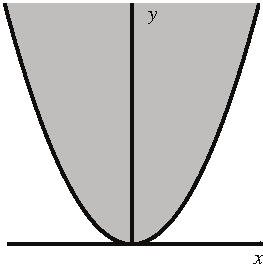
\includegraphics[width=\linewidth]{external/figps-sec71-graph.pdf}
\end{image}%
Graph of a parabola opening up with vertex at the origin. The area above the curve is shaded.\tcblower
\end{figureptx}%
The points \((x, y)\) in the relation \(R\) are the points on the graph of \(y = x^2\) or are in the shaded region. This because for these points, \(y \geq x^2\). One of the shortcomings of this type of graph is that the graph of the equation and the shaded region are actually unbounded and so we can never show the entire graph of this relation. However, it does allow us to see that the points in this relation are either on the parabola defined by the equation \(y = x^2\) or are ``inside'' the parabola.%
\par
\index{directed graph}\index{digraph} When the domain or range of a relation is infinite, we cannot provide a visualization of the entire relation. However, if \(A\) is a (small) finite set, a relation \(R\) on \(A\) can be specified by simply listing all the ordered pairs in \(R\). For example, if \(A = \left\{ {1, 2, 3, 4} \right\}\), then%
\begin{equation*}
R = \left\{ {( {1, 1} ), ( {4, 4} ), ( {1, 3} ), ( {3, 2} ), ( {1, 2} ), ( {2, 1} )} \right\}
\end{equation*}
is a relation on \(A\). A convenient way to represent such a relation is to draw a point in the plane for each of the elements of \(A\) and then for each \(\left( {x, y} \right) \in R\) (or \(x \mathrel{R} y\)), we draw an arrow starting at the point \(x\) and pointing to the point \(y\). If \(\left( {x, x} \right) \in R\) (or \(x \mathrel{R} x\)), we draw a loop at the point \(x\). The resulting diagram is called a \terminology{directed graph} or a \terminology{digraph}. The diagram in \hyperref[x:figure:fig_dirgraph2]{Figure~{\xreffont\ref{x:figure:fig_dirgraph2}}, p.\,\pageref{x:figure:fig_dirgraph2}} is a digraph for the relation \(R\).%
\begin{figureptx}{Directed Graph for a Relation}{x:figure:fig_dirgraph2}{}%
\begin{image}{0.325}{0.35}{0.325}%
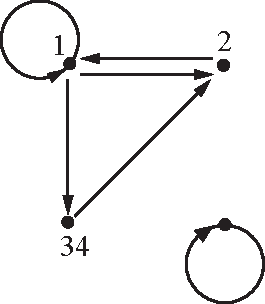
\includegraphics[width=\linewidth]{external/figps-prev72digraph.pdf}
\end{image}%
\tcblower
\end{figureptx}%
\index{vertex}\index{directed graph!vertex}\index{directed edge}\index{directed graph!directed edge} In a directed graph, the points are called the \terminology{vertices}. So each element of \(A\) corresponds to a \terminology{vertex}. The arrows, including the loops, are called the \terminology{directed edges} of the directed graph. We will make use of these directed graphs in the next section when we study equivalence relations.%
\begin{inlineexercise}{The Directed Graph of a Relation.}{x:exercise:prog_directedgraph}%
Let \(A = \{ 1, 2, 3, 4, 5, 6 \}\). Draw a directed graph for the following two relations on the set \(A\). For each relation, it may be helpful to arrange the vertices of \(A\) as shown in \hyperref[x:figure:fig_dirgraph3]{Figure~{\xreffont\ref{x:figure:fig_dirgraph3}}, p.\,\pageref{x:figure:fig_dirgraph3}}.%
\begin{equation*}
R = \{ (x, y) \in A \times A \mid x \text{ divides }  y \}, \qquad T = \{ (x, y) 
\in A \times A \mid x + y \text{ is even }  \}\text{.}
\end{equation*}
%
\begin{figureptx}{Vertices for \(A\)}{x:figure:fig_dirgraph3}{}%
\begin{image}{0.3}{0.4}{0.3}%
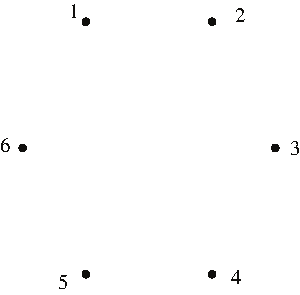
\includegraphics[width=\linewidth]{external/figps-sec71-dirgraph.pdf}
\end{image}%
\tcblower
\end{figureptx}%
\space\hyperlink{g:solution:idm819157672-back}{[Solution]}\end{inlineexercise}%
\end{subsectionptx}
%
%
\typeout{************************************************}
\typeout{Exercises  Exercises}
\typeout{************************************************}
%
\begin{exercises-subsection}{Exercises}{}{Exercises}{}{}{g:exercises:idm819158184}
\begin{divisionexercise}{1}{}{}{x:exercise:exer_sec71-1}%
 Let \(A = \left\{ {a, b, c} \right\}\), \(B = \left\{ {p, q, r} \right\}\), and let \(R\) be the set of ordered pairs defined by \(R = \left\{ {\left( {a, p} \right), \left( {b, q} \right), \left( {c, p} \right), 
\left( {a, q} \right)} \right\}\).%
\begin{enumerate}[font=\bfseries,label=(\alph*),ref=\alph*]
\item{}Use the roster method to list all the elements of \(A \times B\). Explain why \(A \times B\) can be considered to be a relation from \(A\) to \(B\).%
\space\hyperlink{g:answer:idm819418408-back}{[Answer]}\item{}Explain why \(R\) is a relation from \(A\) to \(B\).%
\space\hyperlink{g:answer:idm819061656-back}{[Answer]}\item{}What is the domain of \(R\)? What is the range of \(R\)?%
\space\hyperlink{g:answer:idm819057816-back}{[Answer]}\end{enumerate}
\end{divisionexercise}%
\begin{divisionexercise}{2}{}{}{x:exercise:exer_sec71-2}%
Let \(A = \left\{ {a, b, c} \right\}\) and let \(R = \left\{ {\left( {a, a} \right), \left( {a, c} \right), \left( {b, b} \right), 
\left( {b, c} \right), \left( {c, a} \right), \left( {c, b} \right)} \right\}\) (so \(R\) is a relation on \(A\)). Are the following statements true or false? Explain.%
\begin{enumerate}[font=\bfseries,label=(\alph*),ref=\alph*]
\item{}For each \(x \in A\), \(x \mathrel{R} x\).%
\space\hyperlink{g:answer:idm819055128-back}{[Answer]}\item{}For every \(x, y \in A\), if \(x \mathrel{R} y\), then \(y \mathrel{R} x\).%
\space\hyperlink{g:answer:idm819050648-back}{[Answer]}\item{}For every \(x, y, z \in A\), if \(x \mathrel{R} y\) and \(y \mathrel{R} z\), then \(x \mathrel{R} z\).%
\space\hyperlink{g:answer:idm819053464-back}{[Answer]}\item{}\(R\) is a function from \(A\) to \(A\).%
\space\hyperlink{g:answer:idm819045144-back}{[Answer]}\end{enumerate}
\end{divisionexercise}%
\begin{divisionexercise}{3}{}{}{x:exercise:exer_sec71-3}%
Let  \(A\)  be the set of all female citizens of the United States. Let  \(D\)  be the relation on  \(A\)  defined by%
\begin{equation*}
D = \left\{ { {\left( {x, y} \right) \in A \times A } \mid x\text{  is a daughter of  } y} \right\}\!\text{.}
\end{equation*}
That is,  \(x \mathrel{D} y\) means that  \(x\)  is a daughter of  \(y\).%
\begin{enumerate}[font=\bfseries,label=(\alph*),ref=\alph*]
\item{}Describe those elements of \(A\) that are in the domain of \(D\).%
\space\hyperlink{g:answer:idm819035928-back}{[Answer]}\item{}Describe those elements of \(A\) that are in the range of \(D\).%
\space\hyperlink{g:answer:idm819032728-back}{[Answer]}\item{}Is the relation \(D\) a function from \(A\) to \(A\)? Explain.%
\end{enumerate}
\end{divisionexercise}%
\begin{divisionexercise}{4}{}{}{x:exercise:exer_sec71-4}%
Let  \(U\)  be a nonempty set, and let \(R\) be the ``subset relation'' on \(\mathcal{P}( U )\). That is,%
\begin{equation*}
R = \left\{ { {\left( {S, T} \right) \in \mathcal{P}( U ) \times \mathcal{P}( U ) } 
\mid S \subseteq T} \right\}\!\text{.}
\end{equation*}
%
\begin{enumerate}[font=\bfseries,label=(\alph*),ref=\alph*]
\item{}Write the open sentence \(\left( {S, T} \right) \in R\) using standard subset notation.%
\space\hyperlink{g:answer:idm819024408-back}{[Answer]}\item{}What is the domain of this subset relation, \(R\)?%
\space\hyperlink{g:answer:idm819023256-back}{[Answer]}\item{}What is the range of this subset relation, \(R\)?%
\space\hyperlink{g:answer:idm819028760-back}{[Answer]}\item{}Is \(R\) a function from \(\mathcal{P}( U )\) to \(\mathcal{P}( U )\)? Explain.%
\space\hyperlink{g:answer:idm819022360-back}{[Answer]}\end{enumerate}
\end{divisionexercise}%
\begin{divisionexercise}{5}{}{}{x:exercise:exer_sec71-5}%
Let \(U\) be a nonempty set, and let  \(R\)  be the ``element of'' relation from \(U\) to \(\mathcal{P}\left( U \right)\). That is,%
\begin{equation*}
R = \left\{ { {\left( {x, S} \right) \in U \times \mathcal{P}( U ) } \mid x \in S} 
\right\}\!\text{.}
\end{equation*}
%
\begin{enumerate}[font=\bfseries,label=(\alph*),ref=\alph*]
\item{}What is the domain of this ``element of'' relation, \(R\)?%
\item{}What is the range of this ``element of'' relation, \(R\)?%
\item{}Is \(R\) a function from \(U\) to \(\mathcal{P}( U )\)? Explain.%
\end{enumerate}
\end{divisionexercise}%
\begin{divisionexercise}{6}{}{}{x:exercise:exer_circle-mainmain}%
Let \(S = \left\{ {\left( {x, y} \right) \in \mathbb{R} \times \mathbb{R} 
\mid x^2 + y^2 = 100} \right\}\).%
\begin{enumerate}[font=\bfseries,label=(\alph*),ref=\alph*]
\item\label{x:task:exer_circle-a}Determine the set of all values of \(x\) such that \(\left( {x, 6} \right) \in S\), and determine the set of all values of \(x\) such that \(\left( {x, 9} \right) \in S\).%
\space\hyperlink{g:answer:idm819011864-back}{[Answer]}\item{}Determine the domain and range of the relation \(S\) and write each set using set builder notation.%
\space\hyperlink{g:answer:idm819011096-back}{[Answer]}\item\label{x:task:exer_circle-e}Is the relation \(S\) a function from \(\mathbb{R}\) to \(\mathbb{R}\)? Explain.%
\space\hyperlink{g:answer:idm819007512-back}{[Answer]}\item{}Since \(S\) is a relation on \(\mathbb{R}\), its elements can be graphed in the coordinate plane. Describe the graph of the relation \(S\). Is the graph consistent with your answers in \hyperref[x:task:exer_circle-a]{Task~{\xreffont 6}.{\xreffont\ref{x:task:exer_circle-a}}, p.\,\pageref{x:task:exer_circle-a}} through \hyperref[x:task:exer_circle-e]{Task~{\xreffont 6}.{\xreffont\ref{x:task:exer_circle-e}}, p.\,\pageref{x:task:exer_circle-e}}? Explain.%
\space\hyperlink{g:answer:idm819003544-back}{[Answer]}\end{enumerate}
\end{divisionexercise}%
\begin{divisionexercise}{7}{}{}{x:exercise:exer_semicircle}%
Repeat \hyperlink{x:exercise:exer_circle-mainmain}{Exercise~{\xreffont 6}, p.\,\pageref{x:exercise:exer_circle-mainmain}} using the relation on \(\R\) defined by%
\begin{equation*}
S = \left\{ {\left( {x, y} \right) \in \mathbb{R} \times \mathbb{R} 
\mid y = \sqrt {100 - x^2 } } \right\}\!\text{.}
\end{equation*}
What is the connection between this relation and the relation in \hyperlink{x:exercise:exer_circle-mainmain}{Exercise~{\xreffont 6}, p.\,\pageref{x:exercise:exer_circle-mainmain}}?%
\end{divisionexercise}%
\begin{divisionexercise}{8}{}{}{g:exercise:idm819004440}%
Determine the domain and range of each of the following relations on \(\R\) and sketch the graph of each relation.%
\begin{enumerate}[font=\bfseries,label=(\alph*),ref=\alph*]
\item{}\(R = \left\{ {\left( {x, y} \right) \in \mathbb{R} \times \mathbb{R} 
\mid x^2 + y^2 = 10} \right\}\)%
\item{}\(S = \left\{ {\left( {x, y} \right) \in \mathbb{R} \times \mathbb{R} 
\mid y^2 = x+10} \right\}\)%
\item{}\(T = \left\{ {\left( {x, y} \right) \in \mathbb{R} \times \mathbb{R} 
\mid |x| + |y| = 10} \right\}\)%
\item{}\(R = \left\{ {\left( {x, y} \right) \in \mathbb{R} \times \mathbb{R} 
\mid x^2 =y^2} \right\}\)%
\end{enumerate}
\end{divisionexercise}%
\begin{divisionexercise}{9}{}{}{x:exercise:exer_absvalueless2}%
Let \(\mathrel{R}\) be the relation on \(\Z\) where for all \(a,
b \in \Z\), \(a \mathrel{R} b\) if and only if \(\left| a - b \right| \leq 2\).%
\begin{enumerate}[font=\bfseries,label=(\alph*),ref=\alph*]
\item{}Use set builder notation to describe the relation \(\mathrel{R}\) as a set of ordered pairs.%
\space\hyperlink{g:answer:idm818989592-back}{[Answer]}\item{}Determine the domain and range of the relation \(\mathrel{R}\).%
\space\hyperlink{g:answer:idm818981656-back}{[Answer]}\item{}Use the roster method to specify the set of all integers \(x\) such that \(x \mathrel{R} 5\) and the set of all integers \(x\) such that \(5 \mathrel{R} x\).%
\item{}If possible, find integers \(x\) and \(y\) such that \(x \mathrel{R} 8\), \(8 \mathrel{R} y\), but \(x \mathrel{\not \negthickspace R} y\).%
\item{}If \(b \in \Z\), use the roster method to specify the set of all \(x \in \Z\) such that \(x \mathrel{R} b\).%
\end{enumerate}
\end{divisionexercise}%
\begin{divisionexercise}{10}{}{}{x:exercise:exer_sec71-lessthan}%
Let \(R_{ \lt } = \left\{ { {\left( {x, y} \right) \in \mathbb{R} \times 
\mathbb{R} } \mid x \lt y} \right\}\). This means that \(R_{ \lt }\) is the ``less than'' relation on \(\R\).%
\begin{enumerate}[font=\bfseries,label=(\alph*),ref=\alph*]
\item{}What is the domain of the relation \(R_{ \lt }\)?%
\item{}What is the range of the relation \(R_{ \lt }\)?%
\item{}Is the relation \(R_{ \lt }\) a function from \(\mathbb{R}\) to \(\mathbb{R}\)? Explain.%
\end{enumerate}
Note: Remember that a relation is a set. Consequently, we can talk about one relation being a subset of another relation. Another thing to remember is that the elements of a relation are ordered pairs.%
\end{divisionexercise}%
\begin{activity}{The Inverse of a Relation.}{x:activity:exer_provinginverse}%
\index{inverse of a function}%
\index{function!inverse of}%
\index{inverse of a function}%
\index{function!inverse of}%
In \hyperref[x:section:S_inversefunctions]{Section~{\xreffont\ref{x:section:S_inversefunctions}}, p.\,\pageref{x:section:S_inversefunctions}}, we introduced the \emph{inverse of a function}. If \(A\) and \(B\) are nonempty sets and if \(f:A \to B\) is a function, then the inverse of  \(f\), denoted by  \(f^{ - 1}\), is defined as%
\begin{align*}
f^{ - 1}  \amp = \left\{ { {\left( {b, a} \right) \in B \times A } 
\mid f\left( a \right) = b} \right\}\\
\amp = \left\{ { {\left( {b, a} \right) \in B \times A } \mid \left( {a, b} 
\right) \in f} \right\}\!\text{.}
\end{align*}
Now that we know about relations, we see that  \(f^{ - 1}\)  is always a relation from  \(B\)  to \(A\). The concept of the inverse of a function is actually a special case of the more general concept of the inverse of a relation, which we now define.%
\begin{assemblage}{Definition.}{x:assemblage:inverseofrelation}%
\label{g:notation:idm818967576} Let \(R\) be a relation from the set \(A\) to the set \(B\). The \terminology{inverse of \(\boldsymbol{R}\)}, written \(R^{ - 1}\) and read ``\(R\) inverse,'' is the relation from \(B\) to \(A\) defined by%
\begin{align*}
R^{ - 1} \amp = \left\{ { {\left( {y, x} \right) \in B \times A } \mid 
\left( {x, y} \right) \in R} \right\}\text{ , or }\\
R^{ - 1} \amp = \left\{ { {\left( {y, x} \right) \in B \times A } 
\mid x \mathrel{R} y} \right\}\!\text{.}
\end{align*}
%
\par
That is, \(R^{ - 1}\) is the subset of \(B \times A\) consisting of all ordered pairs \(\left( {y, x} \right)\) such that \(x \mathrel{R} y\).%
\end{assemblage}
For example, let \(D\) be the ``divides'' relation on  \(\mathbb{Z}\).  See \hyperref[x:exercise:prog_dividesrelation]{Progress Check~{\xreffont\ref{x:exercise:prog_dividesrelation}}, p.\,\pageref{x:exercise:prog_dividesrelation}}. So%
\begin{equation*}
D = \left\{ { {\left( {m, n} \right) \in \mathbb{Z} \times \mathbb{Z} } 
\mid m\text{  divides  } n} \right\}\!\text{.}
\end{equation*}
This means that we can write \(m \mid n\) if and only if \(\left( {m, n} \right) 
\in D\). So, in this case,%
\begin{align*}
D^{ - 1}  \amp = \left\{ { {\left( {n, m} \right) \in \mathbb{Z} \times 
\mathbb{Z} } \mid \left( {m, n} \right) \in D} \right\}\\
\amp = \left\{ { {\left( {n, m} \right) \in \mathbb{Z} \times \mathbb{Z} } 
\mid m\text{  divides  } n} \right\}\!\text{.}
\end{align*}
Now, if we would like to focus on the first coordinate instead of the second coordinate in \(D^{ - 1}\), we know that ``\(m\)  divides  \(n\)'' means the same thing as ``\(n\)  is a multiple of  \(m\).'' Hence,%
\begin{equation*}
D^{ - 1}  = \left\{ { {\left( {n, m} \right) \in \mathbb{Z} \times \mathbb{Z} } 
\mid n\text{  is a multiple of  } m} \right\}\!\text{.}
\end{equation*}
%
\par
We can say that the inverse of the ``divides'' relation on  \(\mathbb{Z}\)  is the ``is a multiple of'' relation on  \(\mathbb{Z}\). \hyperref[x:theorem:T_inverserelations]{Theorem~{\xreffont\ref{x:theorem:T_inverserelations}}, p.\,\pageref{x:theorem:T_inverserelations}}, which follows, contains some elementary facts about inverse relations.%
\begin{theorem}{}{}{x:theorem:T_inverserelations}%
Let \(R\) be a relation from the set \(A\) to the set \(B\). Then%
\begin{itemize}[label=\textbullet]
\item{}The domain of \(R^{ - 1}\) is the range of \(R\). That is, \(\text{ dom} \!\left( {R^{ - 1} } \right) = \text{ range} ( R )\).%
\item{}The range of \(R^{ - 1}\) is the domain of \(R\). That is, \(\text{ range} \!\left( {R^{ - 1} } \right) = \text{ dom} ( R )\).%
\item{}The inverse of \(R^{ - 1}\) is \(R\). That is, \(\left( {R^{ - 1} } \right)^{ - 1} = R\).%
\end{itemize}
%
\end{theorem}
To prove the first part of \hyperref[x:theorem:T_inverserelations]{Theorem~{\xreffont\ref{x:theorem:T_inverserelations}}, p.\,\pageref{x:theorem:T_inverserelations}}, observe that the goal is to prove that two sets are equal,%
\begin{equation*}
\text{ dom} \!\left( {R^{ - 1} } \right) = \text{ range} ( R )\text{.}
\end{equation*}
One way to do this is to prove that each is a subset of the other. To prove that \(\text{ dom} \!\left( {R^{ - 1} } \right) \subseteq \text{ range} ( R )\), we can start by choosing an arbitrary element of \(\text{ dom} \!\left( {R^{ - 1} } \right)\).  So let \(y \in \text{ dom} \!\left( {R^{ - 1} } \right)\).  The goal now is to prove that \(y~\in~\text{ range} ( R )\). What does it mean to say that \(y \in \text{ dom} \!\left( {R^{ - 1} } \right)\)?  It means that there exists an \(x \in A\)  such that%
\begin{equation*}
\left( {y, x} \right) \in R^{ - 1}\text{.}
\end{equation*}
Now what does it mean to say that  \(( {y, x} ) \in R^{ - 1}\)? It means that \(( {x, y} ) \in R\). What does this tell us about \(y\)? Complete the proof of the first part of \hyperref[x:theorem:T_inverserelations]{Theorem~{\xreffont\ref{x:theorem:T_inverserelations}}, p.\,\pageref{x:theorem:T_inverserelations}}. Then, complete the proofs of the other two parts of \hyperref[x:theorem:T_inverserelations]{Theorem~{\xreffont\ref{x:theorem:T_inverserelations}}, p.\,\pageref{x:theorem:T_inverserelations}}.%
\end{activity}%
\end{exercises-subsection}
\end{sectionptx}
%
%
\typeout{************************************************}
\typeout{Section 7.2 Equivalence Relations}
\typeout{************************************************}
%
\begin{sectionptx}{Equivalence Relations}{}{Equivalence Relations}{}{}{x:section:S_equivrelations}
%
%
\typeout{************************************************}
\typeout{Beginning Activity  Beginning Activity 1: Properties of Relations}
\typeout{************************************************}
%
\begin{worksheet-subsection}{Beginning Activity 1: Properties of Relations}{}{Beginning Activity 1: Properties of Relations}{}{}{x:worksheet:PA_propsofrelaitons}
In previous mathematics courses, we have worked with the equality relation. For example, let \(R\) be the relation on \(\Z\) defined as follows: For all \(a,
b \in \Z\), \(a \mathrel{R} b\) if and only if \(a = b\). We know this equality relation on \(\Z\) has the following properties:%
\begin{itemize}[label=\textbullet]
\item{}For each \(a \in \Z\), \(a = a\) and so \(a \mathrel{R} a\).%
\item{}For all \(a, b \in \Z\), if \(a = b\), then \(b = a\). That is, if \(a \mathrel{R} b\), then \(b \mathrel{R} a\).%
\item{}For all \(a, b, c \in \Z\), if \(a = b\) and \(b = c\), then \(a = c\). That is, if \(a \mathrel{R} b\) and \(b \mathrel{R} c\), then \(a \mathrel{R} c\).%
\end{itemize}
In mathematics, when something satisfies certain properties, we often ask if other things satisfy the same properties. Before investigating this, we will give names to these properties.%
\begin{assemblage}{Definition.}{x:assemblage:ref-sym-trans}%
Let \(A\) be a nonempty set and let \(R\) be a relation on \(A\).%
\begin{itemize}[label=\textbullet]
\item{}\index{reflexive}\index{relation!reflexive on}The relation \(R\) is \terminology{reflexive on \(\boldsymbol{A}\)} provided that for each \(x \in A\), \(x \mathrel{R} x\) or, equivalently, \(\left( {x, x} \right) \in R\).%
\item{}\index{symmetric}\index{relation!symmetric}The relation \(R\) is \terminology{symmetric} provided that for every \(x,
y \in A\), if \(x \mathrel{R} y\), then \(y \mathrel{R} x\) or, equivalently, for every \(x, y \in A\), if \(\left( {x, y} \right) \in R\), then \(\left( {y, x} \right) \in R\).%
\item{}\index{transitive}\index{relation!transitive}The relation \(R\) is \terminology{transitive} provided that for every \(x, y, z \in A\), if \(x \mathrel{R} y\) and \(y \mathrel{R} z\), then \(x \mathrel{R} z\) or, equivalently, for every \(x, y, z \in A\), if \(\left( {x, y} \right) \in R\) and \(\left( {y, z} \right) \in R\), then \(\left( {x, z} \right) \in R\).%
\end{itemize}
%
\end{assemblage}
Before exploring examples, for each of these properties, it is a good idea to understand what it means to say that a relation does not satisfy the property. So let \(A\) be a nonempty set and let \(R\) be a relation on \(A\).%
\begin{divisionexercise}{1}{}{}{g:exercise:idm818906648}%
Carefully explain what it means to say that the relation \(R\) is not reflexive on the set \(A\).%
\end{divisionexercise}%
\begin{divisionexercise}{2}{}{}{g:exercise:idm818899736}%
Carefully explain what it means to say that the relation \(R\) is not symmetric.%
\end{divisionexercise}%
\begin{divisionexercise}{3}{}{}{g:exercise:idm818900760}%
Carefully explain what it means to say that the relation \(R\) is not transitive.%
\end{divisionexercise}%
To illustrate these properties, we let \(A = \left\{ {1, 2, 3, 4} \right\}\) and define the relations \(R\) and \(T\) on \(A\) as follows:%
\begin{align*}
R \amp = \left\{ {( {1, 1} ), ( {2, 2} ), ( {3, 3} ), ( {4, 4} ), ( {1, 3} ), ( {3, 2} )} \right\}\\
T \amp = \left\{ {( {1, 1} ), ( {1, 4} ), ( {2, 4} ), ( {4, 1} ), ( {4, 2} )} \right\}
\end{align*}
%
\begin{divisionexercise}{4}{}{}{g:exercise:idm818905112}%
Draw a directed graph for the relation \(R\). Then explain why the relation \(R\) is reflexive on \(A\), is not symmetric, and is not transitive.%
\end{divisionexercise}%
\begin{divisionexercise}{5}{}{}{g:exercise:idm818905240}%
Draw a directed graph for the relation \(T\). Is the relation \(T\) reflexive on \(A\)? Is the relation \(T\) symmetric? Is the relation \(T\) transitive? Explain.%
\end{divisionexercise}%
\end{worksheet-subsection}
%
%
\typeout{************************************************}
\typeout{Beginning Activity  Beginning Activity 2: Review of Congruence Modulo \(\boldsymbol{n}\)}
\typeout{************************************************}
%
\begin{worksheet-subsection}{Beginning Activity 2: Review of Congruence Modulo \(\boldsymbol{n}\)}{}{Beginning Activity 2: Review of Congruence Modulo \(\boldsymbol{n}\)}{}{}{x:worksheet:PA_reviewofcongruence}
\begin{divisionexercise}{1}{}{}{g:exercise:idm818898328}%
Let \(a, b \in \mathbb{Z}\) and let \(n \in \mathbb{N}\). On \hyperref[x:assemblage:congruence]{Definition, p.\,\pageref{x:assemblage:congruence}} of \hyperref[x:section:S_directproof]{Section~{\xreffont\ref{x:section:S_directproof}}, p.\,\pageref{x:section:S_directproof}}, we defined what it means to say that \(a\) is congruent to \(b\) modulo \(n\). Write this definition and state two different conditions that are equivalent to the definition.%
\end{divisionexercise}%
\begin{divisionexercise}{2}{}{}{g:exercise:idm818897944}%
Explain why congruence modulo \(n\) is a relation on \(\mathbb{Z}\).%
\end{divisionexercise}%
\begin{divisionexercise}{3}{}{}{g:exercise:idm818898456}%
Carefully review \hyperref[x:theorem:T_modprops]{Theorem~{\xreffont\ref{x:theorem:T_modprops}}, p.\,\pageref{x:theorem:T_modprops}} and the proofs given on \hyperref[x:theorem:T_modprops]{Theorem~{\xreffont\ref{x:theorem:T_modprops}}, p.\,\pageref{x:theorem:T_modprops}} of \hyperref[x:section:S_divalgo]{Section~{\xreffont\ref{x:section:S_divalgo}}, p.\,\pageref{x:section:S_divalgo}}. In terms of the properties of relations introduced in \hyperref[x:worksheet:PA_propsofrelaitons]{Beginning Activity 1, p.\,\pageref{x:worksheet:PA_propsofrelaitons}}, what does this theorem say about the relation of congruence modulo \(n\) on the integers?%
\end{divisionexercise}%
\begin{divisionexercise}{4}{}{}{g:exercise:idm818889112}%
Write a complete statement of \hyperref[x:theorem:T_congtorem]{Theorem~{\xreffont\ref{x:theorem:T_congtorem}}, p.\,\pageref{x:theorem:T_congtorem}} and \hyperref[x:corollary:C_congtorem]{Corollary~{\xreffont\ref{x:corollary:C_congtorem}}, p.\,\pageref{x:corollary:C_congtorem}}.%
\end{divisionexercise}%
\begin{divisionexercise}{5}{}{}{g:exercise:idm818888344}%
Write a proof of the symmetric property for congruence modulo \(n\). That is, prove the following: \begin{quote}%
Let \(a, b \in \mathbb{Z}\) and let \(n \in \mathbb{N}\). If \(a \equiv b \pmod n\), then \(b \equiv a \pmod n\).\end{quote}
%
\end{divisionexercise}%
\end{worksheet-subsection}
%
%
\typeout{************************************************}
\typeout{Subsection  Directed Graphs and Properties of Relations}
\typeout{************************************************}
%
\begin{subsectionptx}{Directed Graphs and Properties of Relations}{}{Directed Graphs and Properties of Relations}{}{}{g:subsection:idm818886680}
In \hyperref[x:section:S_relations]{Section~{\xreffont\ref{x:section:S_relations}}, p.\,\pageref{x:section:S_relations}}, we used directed graphs, or digraphs, to represent relations on finite sets. Three properties of relations were introduced in \hyperref[x:worksheet:PA_propsofrelaitons]{Beginning Activity 1, p.\,\pageref{x:worksheet:PA_propsofrelaitons}} and will be repeated in the following descriptions of how these properties can be visualized on a directed graph.%
\par
Let \(A\) be a nonempty set and let \(R\) be a relation on \(A\).%
\begin{itemize}[label=\textbullet]
\item{}\index{reflexive}\index{relation!reflexive on}The relation \(R\) is \terminology{reflexive on \(\boldsymbol{A}\)} provided that for each \(x \in A\), \(x \mathrel{R} x\) or, equivalently, \(\left( {x, x} \right) \in R\). This means that if a reflexive relation is represented on a digraph, there would have to be a loop at each vertex, as is shown in the following figure. \begin{image}{0.45}{0.1}{0.45}%

\includegraphics[width=\linewidth]{external/figps-reflexive.pdf}
\end{image}%
 %
\item{}\index{symmetric}\index{relation!symmetric}The relation \(R\) is \terminology{symmetric} provided that for every \(x,
y \in A\), if \(x \mathrel{R} y\), then \(y \mathrel{R} x\) or, equivalently, for every \(x, y \in A\), if \(\left( {x, y} \right) \in R\), then \(\left( {y, x} \right) \in R\). This means that if a symmetric relation is represented on a digraph, then anytime there is a directed edge from one vertex to a second vertex, there would be a directed edge from the second vertex to the first vertex, as is shown in the following figure. \begin{image}{0.35}{0.3}{0.35}%

\includegraphics[width=\linewidth]{external/figps-symmetric.pdf}
\end{image}%
 %
\item{}\index{transitive}\index{relation!transitive}The relation \(R\) is \terminology{transitive} provided that for every \(x, y, z \in A\), if \(x \mathrel{R} y\) and \(y \mathrel{R} z\), then \(x \mathrel{R} z\) or, equivalently, for every \(x, y, z \in A\), if \(\left( {x, y} \right) \in R\) and \(\left( {y, z} \right) \in R\), then \(\left( {x, z} \right) \in R\). So if a transitive relation is represented by a digraph, then anytime there is a directed edge from a vertex \(x\) to a vertex \(y\) and a directed edge from \(y\) to a vertex \(z\), there would be a directed edge from \(x\) to \(z\).%
\par
In addition, if a transitive relation is represented by a digraph, then anytime there is a directed edge from a vertex \(x\) to a vertex \(y\) and a directed edge from \(y\) to the vertex \(x\), there would be loops at \(x\) and \(y\). These two situations are illustrated as follows: \begin{image}{0.15}{0.7}{0.15}%
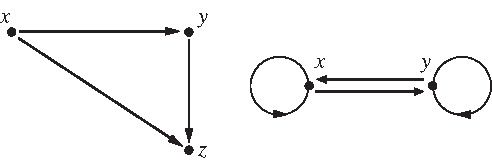
\includegraphics[width=\linewidth]{external/figps-transitive.pdf}
\end{image}%
 %
\end{itemize}
%
\begin{inlineexercise}{Properties of Relations.}{x:exercise:prog_proprelations}%
Let \(A = \{ a, b, c, d \}\) and let \(R\) be the following relation on \(A\):%
\begin{equation*}
R = \{ (a, a), (b, b), (a, c), (c, a), (b, d), (d, b) \}\text{.}
\end{equation*}
%
\par
Draw a directed graph for the relation \(R\) and then determine if the relation \(R\) is reflexive on \(A\), if the relation \(R\) is symmetric, and if the relation \(R\) is transitive.%
\space\hyperlink{g:solution:idm818851224-back}{[Solution]}\end{inlineexercise}%
\end{subsectionptx}
%
%
\typeout{************************************************}
\typeout{Subsection  Definition of an Equivalence Relation}
\typeout{************************************************}
%
\begin{subsectionptx}{Definition of an Equivalence Relation}{}{Definition of an Equivalence Relation}{}{}{g:subsection:idm818847000}
In mathematics, as in real life, it is often convenient to think of two different things as being essentially the same. For example, when you go to a store to buy a cold soft drink, the cans of soft drinks in the cooler are often sorted by brand and type of soft drink. The Coca Colas are grouped together, the Pepsi Colas are grouped together, the Dr. Peppers are grouped together, and so on. When we choose a particular can of one type of soft drink, we are assuming that all the cans are essentially the same. Even though the specific cans of one type of soft drink are physically different, it makes no difference which can we choose. In doing this, we are saying that the cans of one type of soft drink are equivalent, and we are using the mathematical notion of an equivalence relation.%
\par
An equivalence relation on a set is a relation with a certain combination of properties that allow us to sort the elements of the set into certain classes. In this section, we will focus on the properties that define an equivalence relation, and in the next section, we will see how these properties allow us to sort or partition the elements of the set into certain classes.%
\begin{assemblage}{Definition.}{x:assemblage:equivalencerelation}%
Let \(A\) be a nonempty set. A relation \(\sim\) on the set \(A\) is an \terminology{equivalence relation} provided that \(\sim\) is reflexive, symmetric, and transitive. For \(a, b \in A\), if \(\sim\) is an equivalence relation on \(A\) and \(a \sim b\), we say that \(\boldsymbol{a}\) \terminology{is equivalent to \(\boldsymbol{b}\)}.%
\end{assemblage}
Most of the examples we have studied so far have involved a relation on a small finite set. For these examples, it was convenient to use a directed graph to represent the relation. It is now time to look at some other type of examples, which may prove to be more interesting. In these examples, keep in mind that there is a subtle difference between the reflexive property and the other two properties. The reflexive property states that some ordered pairs actually belong to the relation \(R\), or some elements of \(A\) are related. The reflexive property has a universal quantifier and, hence, we must prove that for all \(x \in A\), \(x \mathrel{R} x\). Symmetry and transitivity, on the other hand, are defined by conditional sentences. We often use a direct proof for these properties, and so we start by assuming the hypothesis and then showing that the conclusion must follow from the hypothesis.%
\begin{example}{A Relation that Is Not an Equivalence Relation.}{g:example:idm818835352}%
Let \(M\) be the relation on \(\mathbb{Z}\) defined as follows: \begin{quote}%
For \(a, b \in \mathbb{Z}\), \(a \mathrel{M} b\) if and only if \(a\) is a multiple of \(b\).\end{quote}
%
\par
So \(a \mathrel{M} b\) if and only if there exists a \(k \in \mathbb{Z}\) such that \(a = b k\).%
\begin{itemize}[label=\textbullet]
\item{}The relation \(M\) is reflexive on \(\mathbb{Z}\) since for each \(x \in \mathbb{Z}\), \(x = x \cdot 1\) and, hence, \(x \mathrel{M} x\).%
\item{}Notice that \(4 \mathrel{M} 2\), but \(2 \mathrel{\not \negthickspace M} 4\). So there exist integers \(x\) and \(y\) such that \(x \mathrel{M} y\) but \(y \mathrel{\not \negthickspace M} x\). Hence, the relation \(M\) is not symmetric.%
\item{}Now assume that  \(x \mathrel{M} y\) and  \(y \mathrel{M} z\). Then there exist integers  \(p\)  and  \(q\)  such that%
\begin{equation*}
x = y  p\text{  and  } y = z q\text{.}
\end{equation*}
Using the second equation to make a substitution in the first equation, we see that \(x = z \left( {p q} \right)\). Since  \(p q \in \mathbb{Z}\), we have shown that  \(x\)  is a multiple of  \(z\) and hence  \(x \mathrel{M} z\). Therefore,  \(M\)  is a transitive relation.%
\end{itemize}
%
\end{example}
The relation \(M\) is reflexive on \(\Z\) and is transitive, but since \(M\) is not symmetric, it is not an equivalence relation on \(\Z\).%
\begin{inlineexercise}{A Relation that Is an Equivalence Relation.}{x:exercise:prog_example-equiv}%
Define the relation \(\sim\) on \(\Q\) as follows: For all \(a,
b \in \Q\), \(a \sim b\) if and only if \(a - b \in \Z\). For example:%
\begin{itemize}[label=\textbullet]
\item{}\(\dfrac{3}{4} \sim \dfrac{7}{4}\) since \(\dfrac{3}{4} - \dfrac{7}{4} = -1\) and \(-1 \in \Z\).%
\item{}\(\dfrac{3}{4} \not \sim \dfrac{1}{2}\) since \(\dfrac{3}{4} - \dfrac{1}{2} = \dfrac{1}{4}\) and \(\dfrac{1}{4} \notin \Z\).%
\end{itemize}
%
\par
To prove that \(\sim\) is reflexive on \(\Q\), we note that for all \(a \in \Q\), \(a - a = 0\). Since \(0 \in \Z\), we conclude that \(a \sim a\). Now prove that the relation \(\sim\) is symmetric and transitive, and hence, that \(\sim\) is an equivalence relation on \(\Q\).%
\space\hyperlink{g:solution:idm818815384-back}{[Solution]}\end{inlineexercise}%
\end{subsectionptx}
%
%
\typeout{************************************************}
\typeout{Subsection  Congruence Modulo \(\boldsymbol{n}\)}
\typeout{************************************************}
%
\begin{subsectionptx}{Congruence Modulo \(\boldsymbol{n}\)}{}{Congruence Modulo \(\boldsymbol{n}\)}{}{}{g:subsection:idm819069976}
\index{congruence}%
One of the important equivalence relations we will study in detail is that of congruence modulo \(n\). We reviewed this relation in \hyperref[x:worksheet:PA_reviewofcongruence]{Beginning Activity 2, p.\,\pageref{x:worksheet:PA_reviewofcongruence}}.%
\par
\hyperref[x:theorem:T_modprops]{Theorem~{\xreffont\ref{x:theorem:T_modprops}}, p.\,\pageref{x:theorem:T_modprops}} tells us that congruence modulo \(n\) is an equivalence relation on \(\mathbb{Z}\). Recall that by the Division Algorithm, if \(a \in \mathbb{Z}\), then there exist unique integers \(q\) and \(r\) such that%
\begin{equation*}
a = nq + r \text{  and  } 0 \leq r \lt  n\text{.}
\end{equation*}
%
\par
\hyperref[x:theorem:T_congtorem]{Theorem~{\xreffont\ref{x:theorem:T_congtorem}}, p.\,\pageref{x:theorem:T_congtorem}} and \hyperref[x:corollary:C_congtorem]{Corollary~{\xreffont\ref{x:corollary:C_congtorem}}, p.\,\pageref{x:corollary:C_congtorem}} then tell us that \(a \equiv r \pmod n\). That is, \(a\) is congruent modulo \(n\) to its remainder \(r\) when it is divided by \(n\). When we use the term ``remainder'' in this context, we always mean the remainder \(r\) with \(0 \leq r \lt n\) that is guaranteed by the Division Algorithm. We can use this idea to prove the following theorem.%
\begin{theorem}{}{}{x:theorem:T_congruence-remainder}%
Let \(n \in \mathbb{N}\) and let \(a, b \in \mathbb{Z}\). Then \(a \equiv b \pmod n\) if and only if \(a\) and \(b\) have the same remainder when divided by \(n\).%
\end{theorem}
\begin{proof}{}{g:proof:idm818788776}
Let \(n \in \mathbb{N}\) and let \(a, b \in \mathbb{Z}\). We will first prove that if \(a\) and \(b\) have the same remainder when divided by \(n\), then \(a \equiv b \pmod n\). So assume that \(a\) and \(b\) have the same remainder when divided by \(n\), and let \(r\) be this common remainder. Then, by \hyperref[x:theorem:T_congtorem]{Theorem~{\xreffont\ref{x:theorem:T_congtorem}}, p.\,\pageref{x:theorem:T_congtorem}},%
\begin{equation*}
a \equiv r \pmod n \text{  and  } b \equiv r \pmod n\!\text{.}
\end{equation*}
Since congruence modulo \(n\) is an equivalence relation, it is a symmetric relation. Hence, since \(b \equiv r \pmod n\), we can conclude that \(r \equiv b \pmod n\). Combining this with the fact that \(a \equiv r \pmod n\), we now have%
\begin{equation*}
a \equiv r \pmod n\text{  and  } r \equiv b \pmod n\!\text{.}
\end{equation*}
We can now use the transitive property to conclude that \(a \equiv b \pmod n\). This proves that if \(a\) and \(b\) have the same remainder when divided by \(n\), then \(a \equiv b \pmod n\).%
\par
We will now prove that if \(a \equiv b \pmod n\), then \(a\) and \(b\) have the same remainder when divided by \(n\). Assume that \(a \equiv b \pmod n\), and let \(r\) be the least nonnegative remainder when \(b\) is divided by \(n\). Then \(0 \leq r \lt  n\) and, by \hyperref[x:theorem:T_congtorem]{Theorem~{\xreffont\ref{x:theorem:T_congtorem}}, p.\,\pageref{x:theorem:T_congtorem}},%
\begin{equation*}
b \equiv r \pmod n\!\text{.}
\end{equation*}
Now, using the facts that \(a \equiv b \pmod n\) and \(b \equiv r \pmod n\), we can use the transitive property to conclude that%
\begin{equation*}
a \equiv r \pmod n\!\text{.}
\end{equation*}
This means that there exists an integer \(q\) such that \(a - r = nq\) or that%
\begin{equation*}
a = nq + r\text{.}
\end{equation*}
Since we already know that \(0 \leq r \lt n\), the last equation tells us that \(r\) is the least nonnegative remainder when \(a\) is divided by \(n\). Hence we have proven that if \(a \equiv b \pmod n\), then \(a\) and \(b\) have the same remainder when divided by \(n\).%
\end{proof}
\end{subsectionptx}
%
%
\typeout{************************************************}
\typeout{Subsection  Examples of Other Equivalence Relations}
\typeout{************************************************}
%
\begin{subsectionptx}{Examples of Other Equivalence Relations}{}{Examples of Other Equivalence Relations}{}{}{g:subsection:idm818775080}
\index{equality relation}%
\index{relation!equality}%
\index{identity relation}%
\index{relation!identity}%
%
\begin{enumerate}
\item{}The relation \(\sim\) on \(\Q\) from \hyperref[x:exercise:prog_example-equiv]{Progress Check~{\xreffont\ref{x:exercise:prog_example-equiv}}, p.\,\pageref{x:exercise:prog_example-equiv}} is an equivalence relation.%
\item{}Let \(A\) be a nonempty set. The \terminology{equality relation on \(\boldsymbol{A}\)} is an equivalence relation. This relation is also called the \terminology{identity relation on \(\boldsymbol{A}\)} and is denoted by  \(I_A\), where%
\begin{equation*}
I_A  = \left\{ {\left( {x, x} \right)   \mid x \in A} \right\}\!\text{.}
\end{equation*}
%
\item{}Define the relation \(\sim\) on \(\mathbb{R}\) as follows: \begin{quote}%
For \(a, b \in \mathbb{R}\), \(a \sim b\) if and only if there exists an integer \(k\) such that \(a - b = 2k\pi\).\end{quote}
%
\par
We will prove that the relation \(\sim\) is an equivalence relation on \(\mathbb{R}\). The relation  \(\sim\)  is reflexive on \(\mathbb{R}\) since for each  \(a \in \mathbb{R}\), \(a - a = 0 = 2 \cdot 0 \cdot \pi\).%
\par
Now, let  \(a,
b \in \mathbb{R}\) and assume that  \(a \sim b\). We will prove that  \(b \sim a\). Since  \(a \sim b\), there exists an integer  \(k\)  such that%
\begin{equation*}
a - b = 2k\pi\text{.}
\end{equation*}
By multiplying both sides of this equation by \(-1\), we obtain%
\begin{align*}
( { - 1} )( {a - b} ) \amp = ( { - 1} )( {2k\pi } )\\
b = a \amp = 2( { - k} )\pi\text{.}
\end{align*}
Since  \(- k \in \mathbb{Z}\), the last equation proves that  \(b \sim a\). Hence, we have proven that if  \(a \sim b\), then  \(b \sim a\) and, therefore, the relation  \(\sim\)  is symmetric.%
\par
To prove transitivity, let \(a,
b, c \in \mathbb{R}\) and assume that  \(a \sim b\) and \(b \sim c\). We will prove that  \(a \sim c\). Now, there exist integers  \(k\)  and  \(n\)  such that%
\begin{equation*}
a - b = 2k\pi \text{  and  } b - c = 2n\pi\text{.}
\end{equation*}
By adding the corresponding sides of these two equations, we see that%
\begin{align*}
( {a - b} ) + ( {b - c} ) \amp = 2k\pi  + 2n\pi\\
a - c \amp = 2( {k + n} )\pi
\end{align*}
By the closure properties of the integers, \(k + n \in \mathbb{Z}\). So this proves that \(a \sim c\) and, hence the relation  \(\sim\)  is transitive.%
\par
We have now proven that  \(\sim\)  is an equivalence relation on  \(\mathbb{R}\). This equivalence relation is important in trigonometry. If   \(a \sim b\), then there exists an integer  \(k\)  such that  \(a - b = 2k\pi\) and, hence,  \(a = b + k( {2\pi } )\). Since the sine and cosine functions are periodic with a period of  \(2\pi\), we see that%
\begin{align*}
\sin a \amp = \sin( {b + k( {2\pi } )} ) = \sin b,\text{ and }\\
\cos a \amp = \cos( {b + k( {2\pi } )} ) = \cos b\text{.}
\end{align*}
Therefore, when  \(a \sim b\), each of the trigonometric functions have the same value at  \(a\)  and  \(b\).%
\item{}For an example from Euclidean geometry, we define a relation \(P\) on the set \(\mathcal{L}\) of all lines in the plane as follows: \begin{quote}%
For \(l_1 , l_2 \in \mathcal{L}\), \(l_1 \mathrel{P}l_2\) if and only if \(l_1\) is parallel to \(l_2\) or \(l_1 = l_2\).\end{quote}
 We added the second condition to the definition of \(P\) to ensure that \(P\) is reflexive on \(\mathcal{L}\). Theorems from Euclidean geometry tell us that if \(l_1\) is parallel to \(l_2\), then \(l_2\) is parallel to \(l_1\), and if \(l_1\) is parallel to \(l_2\) and \(l_2\) is parallel to \(l_3\), then \(l_1\) is parallel to \(l_3\). (Drawing pictures will help visualize these properties.) This tells us that the relation \(P\) is reflexive, symmetric, and transitive and, hence, an equivalence relation on \(\mathcal{L}\).%
\end{enumerate}
\begin{inlineexercise}{Another Equivalence Relation.}{x:exercise:prog_anotherequiv}%
Let \(U\) be a finite, nonempty set and let \(\mathcal{P}\left( U \right)\) be the power set of \(U\). Recall that \(\mathcal{P}\left( U \right)\) consists of all subsets of \(U\). (See \hyperref[x:assemblage:D_powerset]{Definition, p.\,\pageref{x:assemblage:D_powerset}}.) Define the relation \(\approx\) on \(\mathcal{P}\left( U \right)\) as follows: \begin{quote}%
For \(A, B \in \mathcal{P}\left( U \right)\), \(A \approx B\) if and only if \(\card(A) = \card(B)\).\end{quote}
 For the definition of the cardinality of a finite set, see \hyperref[x:assemblage:D_cardinality]{Definition, p.\,\pageref{x:assemblage:D_cardinality}}. This relation states that two subsets of \(U\) are equivalent provided that they have the same number of elements. Prove that \(\approx\) is an equivalence relation on the power set \(\mathcal{P}\left( U \right)\).%
\space\hyperlink{g:solution:idm818726568-back}{[Solution]}\end{inlineexercise}%
\end{subsectionptx}
%
%
\typeout{************************************************}
\typeout{Exercises  Exercises}
\typeout{************************************************}
%
\begin{exercises-subsection}{Exercises}{}{Exercises}{}{}{g:exercises:idm818718120}
\begin{divisionexercise}{1}{}{}{x:exercise:exer_sec72-1}%
Let \(A = \left\{ {a, b} \right\}\) and let \(R = \left\{ {\left( {a, b} \right)} \right\}\). Is \(R\) an equivalence relation on \(A\)? If not, is \(R\) reflexive, symmetric, or transitive? Justify all conclusions.%
\space\hyperlink{g:answer:idm818708264-back}{[Answer]}\end{divisionexercise}%
\begin{divisionexercise}{2}{}{}{x:exercise:exer_sec72examples}%
Let \(A = \left\{ {a, b, c} \right\}\). For each of the following, draw a directed graph that represents a relation with the specified properties.%
\begin{enumerate}[font=\bfseries,label=(\alph*),ref=\alph*]
\item{}A relation on \(A\) that is symmetric but not transitive%
\item{}A relation on \(A\) that is transitive but not symmetric%
\item{}A relation on \(A\) that is symmetric and transitive but not reflexive on \(A\)%
\item{}A relation on \(A\) that is not reflexive on \(A\), is not symmetric, and is not transitive%
\item{}A relation on \(A\), other than the identity relation, that is an equivalence relation on \(A\)%
\end{enumerate}
\end{divisionexercise}%
\begin{divisionexercise}{3}{}{}{x:exercise:exer71_notidentity}%
Let  \(A = \left\{ {1, 2, 3, 4, 5} \right\}\). The identity relation on  \(A\)  is%
\begin{equation*}
I_A  = \left\{ {( {1, 1} ), ( {2, 2} ), ( {3, 3} ), ( {4, 4} ), ( {5, 5} )} \right\}\text{.}
\end{equation*}
Determine an equivalence relation on  \(A\)  that is different from  \(I_A\) or explain why this is not possible.%
\space\hyperlink{g:answer:idm818701736-back}{[Answer]}\end{divisionexercise}%
\begin{divisionexercise}{4}{}{}{x:exercise:exer_sec72-2}%
Let \(R = \left\{ { {\left( {x, y} \right) \in \mathbb{R} \times \mathbb{R} } 
\mid \left| x \right| + \left| y \right| = 4} \right\}\). Then \(R\) is a relation on \(\mathbb{R}\). Is \(R\) an equivalence relation on \(\R\)? If not, is \(R\) reflexive, symmetric, or transitive? Justify all conclusions.%
\space\hyperlink{g:answer:idm818693416-back}{[Answer]}\end{divisionexercise}%
\begin{divisionexercise}{5}{}{}{x:exercise:exer_sec72-absvalue}%
A relation \(R\) is defined on \(\Z\) as follows: For all \(a,
b \in \Z\), \(a \mathrel{R} b\) if and only if \(\left| a - b \right| \leq 3\). Is \(R\) an equivalence relation on \(\R\)? If not, is \(R\) reflexive, symmetric, or transitive? Justify all conclusions.%
\end{divisionexercise}%
\begin{divisionexercise}{6}{}{}{x:exercise:exer_equivrelwithfunction}%
Let  \(f\x \mathbb{R} \to \mathbb{R}\) be defined by \(f( x ) = x^2  - 4\) for each  \(x \in \mathbb{R}\). Define a relation  \(\sim\)  on  \(\mathbb{R}\) as follows:%
\begin{equation*}
\text{ For } a, b \in \R,  a \sim b \text{ if and only if } f( a ) = f( b )\text{.}
\end{equation*}
%
\begin{enumerate}[font=\bfseries,label=(\alph*),ref=\alph*]
\item\label{x:task:exer_equivrelwithfunctiona}Is the relation \(\sim\) an equivalence relation on \(\mathbb{R}\)? Justify your conclusion.%
\space\hyperlink{g:answer:idm818683944-back}{[Answer]}\item{}Determine all real numbers in the set \(C = \left\{ { {x \in \R } \mid x \sim 5} \right\}\).%
\space\hyperlink{g:answer:idm818665768-back}{[Answer]}\end{enumerate}
\end{divisionexercise}%
\begin{divisionexercise}{7}{}{}{x:exercise:exer_equivrelwithfunction2}%
Repeat \hyperlink{x:exercise:exer_equivrelwithfunction}{Exercise~{\xreffont 6}, p.\,\pageref{x:exercise:exer_equivrelwithfunction}} using the function \(f\x \mathbb{R} \to \mathbb{R}\) that is defined by \(f( x ) = x^2 - 3x - 7\) for each \(x \in \mathbb{R}\).%
\end{divisionexercise}%
\begin{divisionexercise}{8}{}{}{g:exercise:idm818662312}%
Complete the following.%
\begin{enumerate}[font=\bfseries,label=(\alph*),ref=\alph*]
\item{}Repeat \hyperref[x:task:exer_equivrelwithfunctiona]{Task~{\xreffont 6}.{\xreffont\ref{x:task:exer_equivrelwithfunctiona}}, p.\,\pageref{x:task:exer_equivrelwithfunctiona}} using the function \(f\x \mathbb{R} \to \mathbb{R}\) that is defined by \(f( x ) = \sin x\) for each \(x \in \mathbb{R}\).%
\item{}Determine all real numbers in the set \(C = \left\{ { {x \in \R } \mid x \sim \pi } 
\right\}\).%
\end{enumerate}
\end{divisionexercise}%
\begin{divisionexercise}{9}{}{}{x:exercise:exer_sec72-diffQ}%
Define the relation \(\sim\) on \(\Q\) as follows: For \(a,
b \in \Q\), \(a \sim b\) if and only if \(a - b \in \Z\). In \hyperref[x:exercise:prog_example-equiv]{Progress Check~{\xreffont\ref{x:exercise:prog_example-equiv}}, p.\,\pageref{x:exercise:prog_example-equiv}}, we showed that the relation \(\sim\) is an equivalence relation on \(\Q\).%
\begin{enumerate}[font=\bfseries,label=(\alph*),ref=\alph*]
\item{}List four different elements of the set \(C = \left\{ { {x \in \Q } \mid x \sim 
\dfrac{5}{7} } \right\}\).%
\item{}Use set builder notation (without using the symbol \(\sim\)) to specify the set \(C\).%
\item{}Use the roster method to specify the set \(C\).%
\end{enumerate}
\end{divisionexercise}%
\begin{divisionexercise}{10}{}{}{x:exercise:exer_oneequivonenot}%
Let \(\sim\) and \(\approx\) be relations on \(\Z\) defined as follows:%
\begin{itemize}[label=\textbullet]
\item{}For \(a, b \in \Z\), \(a \sim b\) if and only if 2 divides \(a + b\).%
\item{}For \(a, b \in \Z\), \(a \approx b\) if and only if 3 divides \(a + b\).%
\end{itemize}
%
\begin{enumerate}[font=\bfseries,label=(\alph*),ref=\alph*]
\item{}Is \(\sim\) an equivalence relation on \(\Z\)? If not, is this relation reflexive, symmetric, or transitive?%
\space\hyperlink{g:answer:idm818646952-back}{[Answer]}\item{}Is \(\approx\) an equivalence relation on \(\Z\)? If not, is this relation reflexive, symmetric, or transitive?%
\end{enumerate}
\end{divisionexercise}%
\begin{divisionexercise}{11}{}{}{g:exercise:idm818639016}%
Let \(U\) be a finite, nonempty set and let \(\mathcal{P}( U )\) be the power set of \(U\). That is, \(\mathcal{P} ( U )\) is the set of all subsets of \(U\). Define the relation \(\sim\) on \(\mathcal{P}( U )\) as follows: For \(A, B \in \mathcal{P}( U )\), \(A \sim B\) if and only if \(A \cap B = \emptyset\). That is, the ordered pair \(\left( {A, B} \right)\) is in the relation \(\sim\) if and only if \(A\) and \(B\) are disjoint. Is the relation \(\sim\) an equivalence relation on \(\mathcal{P}( U )\)? If not, is it reflexive, symmetric, or transitive? Justify all conclusions.%
\end{divisionexercise}%
\begin{divisionexercise}{12}{}{}{x:exercise:exer_sec72-powerset}%
Let \(U\) be a nonempty set and let \(\mathcal{P} ( U )\) be the power set of \(U\). That is, \(\mathcal{P} \left( U \right)\) is the set of all subsets of \(U\). For \(A\) and \(B\) in \(\mathcal{P} ( U )\), define \(A \sim B\) to mean that there exists a bijection \(f:A \to B\). Prove that \(\sim\) is an equivalence relation on \(\mathcal{P} ( U )\).%
\par
Use results from \hyperref[x:section:S_compositionoffunctions]{Section~{\xreffont\ref{x:section:S_compositionoffunctions}}, p.\,\pageref{x:section:S_compositionoffunctions}} and \hyperref[x:section:S_inversefunctions]{Section~{\xreffont\ref{x:section:S_inversefunctions}}, p.\,\pageref{x:section:S_inversefunctions}}.%
\end{divisionexercise}%
\begin{divisionexercise}{13}{}{}{x:exercise:exer_modequivrel}%
Let \(\sim\) and \(\approx\) be relations on \(\Z\) defined as follows:%
\begin{itemize}[label=\textbullet]
\item{}For \(a, b \in \Z\), \(a \sim b\) if and only if \(2a + 3b \equiv 0 \pmod 5\).%
\item{}For \(a, b \in \Z\), \(a \approx b\) if and only if \(a + 3b \equiv 0 \pmod 5\).%
\end{itemize}
%
\begin{enumerate}[font=\bfseries,label=(\alph*),ref=\alph*]
\item{}Is \(\sim\) an equivalence relation on \(\Z\)? If not, is this relation reflexive, symmetric, or transitive?%
\item{}Is \(\approx\) an equivalence relation on \(\Z\)? If not, is this relation reflexive, symmetric, or transitive?%
\end{enumerate}
\end{divisionexercise}%
\begin{divisionexercise}{14}{}{}{x:exercise:exer72-signed}%
Let \(\sim\) and \(\approx\) be relations on \(\R\) defined as follows:%
\begin{itemize}[label=\textbullet]
\item{}For \(x, y \in \R\), \(x \sim y\) if and only if \(xy \geq 0\).%
\item{}For \(x, y \in \R\), \(x \approx y\) if and only if \(xy \leq 0\).%
\end{itemize}
%
\begin{enumerate}[font=\bfseries,label=(\alph*),ref=\alph*]
\item{}Is \(\sim\) an equivalence relation on \(\R\)? If not, is this relation reflexive, symmetric, or transitive?%
\item{}Is \(\approx\) an equivalence relation on \(\R\)? If not, is this relation reflexive, symmetric, or transitive?%
\end{enumerate}
\end{divisionexercise}%
\begin{divisionexercise}{15}{}{}{x:exercise:exer_sec72-circles}%
Define the relation  \(\approx\) on \(\mathbb{R} \times \mathbb{R}\) as follows: For \(\left( {a, b} \right), \left( {c, d} \right) \in \mathbb{R} \times \mathbb{R}\), \(\left( {a, b} \right) \approx \left( {c, d} \right)\) if and only if \(a^2  + b^2  = c^2  + d^2\).%
\begin{enumerate}[font=\bfseries,label=(\alph*),ref=\alph*]
\item{}Prove that \(\approx\) is an equivalence relation on \(\mathbb{R} \times \mathbb{R}\).%
\item{}List  four  different elements of the set%
\begin{equation*}
C = \left\{ { {\left( {x, y} \right) \in \mathbb{R} \times \mathbb{R} } \mid                 \left( {x, y} \right) \approx \left( {4, 3} \right)} \right\}\text{.}
\end{equation*}
%
\item{}Give a geometric description of the set \(C\).%
\space\hyperlink{g:answer:idm818603432-back}{[Answer]}\end{enumerate}
\end{divisionexercise}%
\begin{divisionexercise}{16}{Evaluation of Proofs.}{}{g:exercise:idm818596776}%
See the instructions for \hyperlink{x:exercise:exer_proofeval}{Exercise~{\xreffont 19}, p.\,\pageref{x:exercise:exer_proofeval}} from \hyperref[x:section:S_directproof]{Section~{\xreffont\ref{x:section:S_directproof}}, p.\,\pageref{x:section:S_directproof}}.%
\begin{enumerate}[font=\bfseries,label=(\alph*),ref=\alph*]
\item{}%
\begin{descriptionlist}
\begin{dlinarrow}{Proposition}{g:li:idm818597800}%
Let \(R\) be a relation on a set \(A\). If \(R\) is symmetric and transitive, then \(R\) is reflexive.%
\end{dlinarrow}%
\begin{dlinarrow}{Proof}{g:li:idm818597672}%
Let \(x, y \in A\). If \(x \mathrel{R} y\), then \(y \mathrel{R} x\) since \(R\) is symmetric. Now, \(x \mathrel{R} y\) and \(y \mathrel{R} x\), and since \(R\) is transitive, we can conclude that \(x \mathrel{R} x\). Therefore, \(R\) is reflexive.%
\end{dlinarrow}%
\end{descriptionlist}
%
\item{}%
\begin{descriptionlist}
\begin{dlinarrow}{Proposition}{g:li:idm818595368}%
Let \(\sim\) be a relation on \(\Z\) where for all \(a,
b \in \Z\), \(a \sim b\) if and only if \(\left( a + 2b \right) \equiv 0 \pmod 3\). The relation \(\sim\) is an equivalence relation on \(\Z\).%
\end{dlinarrow}%
\begin{dlinarrow}{Proof}{g:li:idm818588200}%
Assume \(a \sim a\). Then \(\left( a + 2a \right) \equiv 0 \pmod 3\) since%
\par
\(\left( 3a \right) \equiv 0 \pmod 3\). Therefore, \(\sim\) is reflexive on \(\Z\). In addition, if \(a \sim b\), then \(\left( a + 2b \right) \equiv 0 \pmod 3\), and if we multiply both sides of this congruence by 2, we get%
\begin{align*}
2\left( a + 2b \right) \amp \equiv 2 \cdot 0 \pmod 3\\
\left( 2a + 4b \right) \amp \equiv 0 \pmod 3\\
\left( 2a + b \right) \amp \equiv 0 \pmod 3\\
\left( b + 2a \right) \amp \equiv 0 \pmod 3\text{.}
\end{align*}
%
\par
This means that \(b \sim a\) and hence, \(\sim\) is symmetric.%
\par
We now assume that \(\left( a + 2b \right) \equiv 0\pmod 3\) and \(\left( b + 2c \right) \equiv 0\pmod 3\). By adding the corresponding sides of these two congruences, we obtain%
\begin{align*}
\left( a + 2b \right) + \left( b + 2c \right) \amp \equiv 0 + 0 \pmod 3\\
\left( a + 3b + 2c \right) \amp \equiv 0 \pmod 3\\
\left( a + 2c \right) \amp \equiv 0 \pmod 3\text{.}
\end{align*}
%
\par
Hence, the relation \(\sim\) is transitive and we have proved that \(\sim\) is an equivalence relation on \(\Z\).%
\end{dlinarrow}%
\end{descriptionlist}
%
\end{enumerate}
\end{divisionexercise}%
\begin{activity}{Other Types of Relations.}{g:activity:idm818578728}%
\index{circular relation}%
\index{relation!circular}%
In this section, we focused on the properties of a relation that are part of the definition of an equivalence relation. However, there are other properties of relations that are of importance. We will study two of these properties in this activity.%
\par
A relation \(R\) on a set \(A\) is a \terminology{circular relation} provided that for all \(x\), \(y\), and \(z\) in \(A\), if \(x \mathrel{R} y\) and \(y \mathrel{R} z\), then \(z \mathrel{R} x\).%
\begin{enumerate}[font=\bfseries,label=(\alph*),ref=\alph*]
\item{}Carefully explain what it means to say that a relation \(R\) on a set \(A\) is not circular.%
\item{}Let \(A = \{ 1, 2, 3 \}\). Draw a directed graph of a relation on \(A\) that is circular and draw a directed graph of a relation on \(A\) that is not circular.%
\item{}Let \(A = \{ 1, 2, 3 \}\). Draw a directed graph of a relation on \(A\) that is circular and not transitive and draw a directed graph of a relation on \(A\) that is transitive and not circular.%
\item{}Prove the following proposition: \begin{quote}%
A relation \(R\) on a set \(A\) is an equivalence relation if and only if it is reflexive and circular.\end{quote}
%
\item{}\index{antisymmetric relation}%
\index{relation!antisymmetric}%
A relation \(R\) on a set \(A\) is an \terminology{antisymmetric relation} provided that for all \(x, y \in A\), if \(x \mathrel{R} y\) and \(y \mathrel{R} x\), then \(x = y\).%
\par
Carefully explain what it means to say that a relation on a set \(A\) is not antisymmetric.%
\item{}Let \(A = \{ 1, 2, 3 \}\). Draw a directed graph of a relation on \(A\) that is antisymmetric and draw a directed graph of a relation on \(A\) that is not antisymmetric.%
\item{}Are the following propositions true or false? Justify all conclusions.%
\begin{enumerate}[font=\bfseries,label=(\roman*),ref=\theenumi.\roman*]
\item{}If a relation \(\mathrel{R}\) on a set \(A\) is both symmetric and antisymmetric, then \(\mathrel{R}\) is transitive.%
\item{}If a relation \(\mathrel{R}\) on a set \(A\) is both symmetric and antisymmetric, then \(\mathrel{R}\) is reflexive.%
\end{enumerate}
\end{enumerate}
\end{activity}%
\end{exercises-subsection}
\end{sectionptx}
%
%
\typeout{************************************************}
\typeout{Section 7.3 Equivalence Classes}
\typeout{************************************************}
%
\begin{sectionptx}{Equivalence Classes}{}{Equivalence Classes}{}{}{x:section:S_equivclasses}
%
%
\typeout{************************************************}
\typeout{Beginning Activity  Beginning Activity 1: Sets Associated with a Relation}
\typeout{************************************************}
%
\begin{worksheet-subsection}{Beginning Activity 1: Sets Associated with a Relation}{}{Beginning Activity 1: Sets Associated with a Relation}{}{}{x:worksheet:PA_setswithrelation}
As was indicated in \hyperref[x:section:S_equivrelations]{Section~{\xreffont\ref{x:section:S_equivrelations}}, p.\,\pageref{x:section:S_equivrelations}}, an equivalence relation on a set \(A\) is a relation with a certain combination of properties (reflexive, symmetric, and transitive) that allow us to sort the elements of the set into certain classes. This is done by means of certain subsets of \(A\) that are associated with the e lements of the set \(A\). This will be illustrated with the following example. Let \(A = \left\{ {a, b, c, d, e} \right\}\), and let \(R\) be the relation on the set \(A\) defined as follows:%
\begin{align*}
a \amp \mathrel{R} a  \amp b \amp \mathrel{R} b  \amp c \amp \mathrel{R} c  \amp d \amp \mathrel{R} d   \amp e \amp \mathrel{R} e\\
a \amp \mathrel{R} b  \amp b \amp \mathrel{R} a  \amp b \amp \mathrel{R} e  \amp e \amp \mathrel{R} b\\
a \amp \mathrel{R} e  \amp e \amp \mathrel{R} a  \amp c \amp \mathrel{R} d  \amp d \amp \mathrel{R} c
\end{align*}
%
\par
For each \(y \in A\), define the subset \(R[y]\) of \(A\) as follows:%
\begin{equation*}
R[y] = \left\{ x \in A \mid x \mathrel{R} y \right\}\text{.}
\end{equation*}
That is, \(R[y]\) consists of those elements in \(A\) such that \(x \mathrel{R} y\). For example, using \(y = a\), we see that \(a \mathrel{R} a\), \(b \mathrel{R} a\), and \(e \mathrel{R} a\), and so \(R[a] = \{ a, b, e \}\).%
\begin{divisionexercise}{1}{}{}{g:exercise:idm818543016}%
Determine \(R[b]\), \(R[c]\), \(R[d]\), and \(R[e]\).%
\end{divisionexercise}%
\begin{divisionexercise}{2}{}{}{g:exercise:idm818539816}%
Draw a directed graph for the relation \(R\) and explain why \(R\) is an equivalence relation on \(A\).%
\end{divisionexercise}%
\begin{divisionexercise}{3}{}{}{g:exercise:idm818545960}%
Which of the sets \(R[ a ]\), \(R[ b ]\), \(R[ c ]\), \(R[ d ]\), and \(R[ e ]\) are equal?%
\end{divisionexercise}%
\begin{divisionexercise}{4}{}{}{g:exercise:idm818541352}%
Which of the sets \(R[ a ]\), \(R[ b ]\), \(R[ c ]\), \(R[ d ]\), and \(R[ e ]\) are disjoint?%
\end{divisionexercise}%
As we will see in this section, the relationships between these sets are typical for an equivalence relation. The following example will show how different this can be for a relation that is not an equivalence relation.%
\par
Let \(A = \left\{ {a, b, c, d, e} \right\}\), and let \(S\) be the relation on the set \(A\) defined as follows:%
\begin{align*}
b \amp \mathrel{S} b  \amp c \amp \mathrel{S} c  \amp d \amp \mathrel{S} d   \amp e \amp \mathrel{S} e\\
a \amp \mathrel{S} b  \amp a \amp \mathrel{S} d  \amp b \amp \mathrel{S} c\\
c \amp \mathrel{S} d  \amp d \amp \mathrel{S} c
\end{align*}
\begin{divisionexercise}{5}{}{}{g:exercise:idm818536232}%
Draw a digraph that represents the relation \(S\) on \(A\). Explain why \(S\) is not an equivalence relation on \(A\).%
\end{divisionexercise}%
%
\par
For each \(y \in A\), define the subset \(S[y]\) of \(A\) as follows:%
\begin{equation*}
S[ y ] = \left\{ { {x \in A } \mid x \mathrel{S} y} \right\} = \left\{ { {x \in A } 
\mid \left( {x, y} \right) \in S} \right\}\text{.}
\end{equation*}
%
\par
For example, using \(y = b\), we see that \(S[b] = \{ a, b \}\) since \((a, b) \in S\) and \((b, b) \in S\). In addition, we see that \(S[a] = \emptyset\) since there is no \(x \in A\) such that \((x, a) \in S\).%
\begin{divisionexercise}{6}{}{}{g:exercise:idm818794792}%
Determine \(S[ c ]\), \(S[ d ]\), and \(S[ e ]\).%
\end{divisionexercise}%
\begin{divisionexercise}{7}{}{}{g:exercise:idm818933784}%
Which of the sets \(S[ a ]\), \(S[ b ]\), \(S[ c ]\), \(S[ d ]\), and \(S[ e ]\) are equal?%
\end{divisionexercise}%
\begin{divisionexercise}{8}{}{}{g:exercise:idm818510728}%
Which of the sets \(S[ b ]\), \(S[ c ]\), \(S[ d ]\), and \(S[ e ]\) are disjoint?%
\end{divisionexercise}%
\end{worksheet-subsection}
%
%
\typeout{************************************************}
\typeout{Beginning Activity  Beginning Activity 2: Congruence Modulo 3}
\typeout{************************************************}
%
\begin{worksheet-subsection}{Beginning Activity 2: Congruence Modulo 3}{}{Beginning Activity 2: Congruence Modulo 3}{}{}{x:worksheet:PA_congruencemodulo3}
An important equivalence relation that we have studied is congruence modulo \(n\) on the integers. We can also define subsets of the integers based on congruence modulo \(n\). We will illustrate this with congruence modulo 3. For example, we can define \(C[0]\) to be the set of all integers \(a\) that are congruent to 0 modulo 3. That is,%
\begin{equation*}
C[ 0 ] = \left\{ { {a \in \mathbb{Z} } \mid a \equiv 0 \pmod 3} \right\}\!\text{.}
\end{equation*}
%
\par
Since an integer \(a\) is congruent to 0 modulo 3 if and only if 3 divides \(a\), we can use the roster method to specify this set as follows:%
\begin{equation*}
C[0] = \left\{  \ldots, -9, -6, -3, 0, 3, 6, 9, \ldots \right\}\text{.}
\end{equation*}
%
\begin{divisionexercise}{1}{}{}{g:exercise:idm818503048}%
Use the roster method to specify each of the following sets:%
\begin{enumerate}[font=\bfseries,label=(\alph*),ref=\alph*]
\item\label{x:task:PA_congruencemodulo3-2}The set \(C[ 1 ]\) of all integers \(a\) that are congruent to 1 modulo 3. That is, \(C[ 1 ] = \left\{ { {a \in \mathbb{Z} } \mid a \equiv 1 \pmod 3} \right\}\!\).%
\item\label{x:task:PA_congruencemodulo3-3}The set \(C[ 2 ]\) of all integers \(a\) that are congruent to 2 modulo 3. That is, \(C[ 2 ] = \left\{ { {a \in \mathbb{Z} } \mid a \equiv 2 \pmod 3} \right\}\!\).%
\item{}The set \(C[ 3 ]\) of all integers \(a\) that are congruent to 3 modulo 3. That is, \(C[ 3 ] = \left\{ { {a \in \mathbb{Z} } \mid a \equiv 3 \pmod 3} \right\}\!\).%
\end{enumerate}
\end{divisionexercise}%
\begin{divisionexercise}{2}{}{}{g:exercise:idm818503176}%
Now consider the three sets, \(C[ 0 ]\), \(C[ 1 ]\), and \(C[ 2 ]\).%
\begin{enumerate}[font=\bfseries,label=(\alph*),ref=\alph*]
\item{}Determine the intersection of any two of these sets. That is, determine \(C[ 0 ] \cap C[ 1 ]\), \(C[ 0 ] \cap C[ 2 ]\), and \(C[ 1 ] \cap C[ 2 ]\).%
\item\label{x:task:PA_congruencemodulo3-5b}Let \(n = 734\). What is the remainder when \(n\) is divided by 3? Which of the three sets, if any, contains \(n = 734\)?%
\item{}Repeat \hyperref[x:task:PA_congruencemodulo3-5b]{Task~{\xreffont 2}.{\xreffont\ref{x:task:PA_congruencemodulo3-5b}}, p.\,\pageref{x:task:PA_congruencemodulo3-5b}} for \(n = 79\) and for \(n=-79\).%
\item{}Do you think that \(C[ 0 ] \cup C[ 1 ] \cup C[ 2 ] = \mathbb{Z}\)? Explain.%
\item{}Is the set \(C[3]\) equal to one of the sets \(C[0], C[1]\), or \(C[2]\)?%
\item{}We can also define \(C[4] = \left\{ { {a \in \mathbb{Z} } \mid a \equiv 4 \pmod 3} \right\}\!\). Is this set equal to any of the previous sets we have studied in this part? Explain.%
\end{enumerate}
\end{divisionexercise}%
\end{worksheet-subsection}
%
%
\typeout{************************************************}
\typeout{Subsection  The Definition of an Equivalence Class}
\typeout{************************************************}
%
\begin{subsectionptx}{The Definition of an Equivalence Class}{}{The Definition of an Equivalence Class}{}{}{g:subsection:idm818495752}
We have indicated that an equivalence relation on a set is a relation with a certain combination of properties (reflexive, symmetric, and transitive) that allow us to sort the elements of the set into certain classes. We saw this happen in the beginning  activities. We can now illustrate specifically what this means. For example, in \hyperref[x:worksheet:PA_congruencemodulo3]{Beginning Activity 2, p.\,\pageref{x:worksheet:PA_congruencemodulo3}}, we used the equivalence relation of congruence modulo 3 on \(\mathbb{Z}\) to construct the following three sets:%
\begin{align*}
C[ 0 ] \amp = \left\{ { {a \in \mathbb{Z} } \mid a \equiv 0 \pmod 3} \right\}\!,\\
C[ 1 ] \amp = \left\{ { {a \in \mathbb{Z} } \mid a \equiv 1 \pmod 3} \right\}\!,\text{ and }\\
C[ 2 ] \amp = \left\{ { {a \in \mathbb{Z} } \mid a \equiv 2 \pmod 3} \right\}\!\text{.}
\end{align*}
%
\par
The main results that we want to use now are \hyperref[x:theorem:T_congtorem]{Theorem~{\xreffont\ref{x:theorem:T_congtorem}}, p.\,\pageref{x:theorem:T_congtorem}} and \hyperref[x:corollary:C_congtorem]{Corollary~{\xreffont\ref{x:corollary:C_congtorem}}, p.\,\pageref{x:corollary:C_congtorem}}. This corollary tells us that for any \(a \in \mathbb{Z}\), \(a\) is congruent to precisely one of the integers 0, 1, or 2. Consequently, the integer \(a\) must be congruent to 0, 1, or 2, and it cannot be congruent to two of these numbers. Thus%
\begin{enumerate}
\item{}For each \(a \in \mathbb{Z}\), \(a \in C[ 0 ]\), \(a \in C[ 1 ]\), or \(a \in C[ 2 ]\); and%
\item{}\(C[ 0 ] \cap C[ 1 ] = \emptyset\), \(C[ 0 ] \cap C[ 2 ] = \emptyset\) , and \(C[ 1 ] \cap C[ 2 ] = \emptyset\).%
\end{enumerate}
%
\par
This means that the relation of congruence modulo 3 sorts the integers into three distinct sets, or classes, and that each pair of these sets have no elements in common. So if we use a rectangle to represent \(\mathbb{Z}\), we can divide that rectangle into three smaller rectangles, corresponding to \(C[ 0 ]\), \(C[ 1 ]\), and \(C[ 2 ]\), and we might picture this situation as follows:%
\begin{center}%
{\tabularfont%
\begin{tabular}{lll}
\textbf{}&\textbf{The Integers}&\textbf{}\tabularnewline\hrulemedium
\multicolumn{1}{lB}{\tablecelllines{l}{m}
{\(C[ 0 ]\) consisting\\
of all integers with a\\
remainder of 0 when\\
divided by 3}
}&\multicolumn{1}{lB}{\tablecelllines{l}{m}
{\(C[ 1 ]\) consisting\\
of all integers with a\\
remainder of 1 when\\
divided by 3}
}&\tablecelllines{l}{m}
{\(C[ 2 ]\) consisting\\
of all integers with a\\
remainder of 2 when\\
divided by 3}

\end{tabular}
}%
\end{center}%
Each integer is in exactly one of the three sets \(C[ 0 ]\), \(C[ 1 ]\), or \(C[ 2 ]\), and two integers are congruent modulo 3 if and only if they are in the same set. We will see that, in a similar manner, if \(n\) is any natural number, then the relation of congruence modulo \(n\) can be used to sort the integers into \(n\) classes. We will also see that in general, if we have an equivalence relation \(R\) on a set \(A\), we can sort the elements of the set \(A\) into classes in a similar manner.%
\begin{assemblage}{Definition.}{x:assemblage:equivalenceclass}%
\label{g:notation:idm818472584} Let \(\sim\) be an equivalence relation on a nonempty set \(A\). For each \(a \in A\), the \terminology{equivalence class of \(\boldsymbol{a}\)} determined by \(\sim\) is the subset of \(A\), denoted by \([ a ]\), consisting of all the elements of \(A\) that are equivalent to \(a\). That is,%
\begin{equation*}
[ a ] = \left\{ { {x \in A } \mid x \sim a} \right\}\!\text{.}
\end{equation*}
%
\par
We read \([ a ]\) as ``the equivalence class of \(a\)'' or as ``bracket \(a\).''%
\end{assemblage}
\begin{paragraphs}{Notes.}{g:paragraphs:idm818457096}%
%
\begin{enumerate}
\item{}We use the notation \([ a ]\) when only one equivalence relation is being used. If there is more than one equivalence relation, then we need to distinguish between the equivalence classes for each relation. We often use something like \([ a ]_{ \sim}\), or if \(R\) is the name of the relation, we can use \(R[ a ]\) or \([a]_R\) for the equivalence class of \(a\) determined by \(R\). In any case, always remember that when we are working with any equivalence relation on a set \(A\) if \(a \in A\), then \emph{the equivalence class \([ a ]\) is a subset of \(A\).}%
\item{}We know that each integer has an equivalence class for the equivalence relation of congruence modulo 3. But as we have seen, there are really only three \emph{distinct} equivalence classes. Using the notation from the definition, they are:%
\begin{align*}
[0] \amp = \left\{ a \in \Z \mid a \equiv 0 \pmod 3 \right\}, \amp  [1] \amp = \left\{ a \in \Z \mid a \equiv 1 \pmod 3 \right\}, \text{ and }\\
[2] \amp = \left\{ a \in \Z \mid a \equiv 2 \pmod 3 \right\}\text{.}
\end{align*}
%
\end{enumerate}
%
\end{paragraphs}%
\begin{inlineexercise}{Equivalence Classes from Beginning Activity 1.}{x:exercise:prog_prev73}%
Without using the terminology at that time, we actually determined the equivalence classes of the equivalence relation \(R\) in \hyperref[x:worksheet:PA_setswithrelation]{Beginning Activity 1, p.\,\pageref{x:worksheet:PA_setswithrelation}}. What are the distinct equivalence classes for this equivalence relation?%
\space\hyperlink{g:solution:idm818453640-back}{[Solution]}\end{inlineexercise}%
\end{subsectionptx}
%
%
\typeout{************************************************}
\typeout{Subsection  Congruence Modulo \(\boldsymbol{n}\) and Congruence Classes}
\typeout{************************************************}
%
\begin{subsectionptx}{Congruence Modulo \(\boldsymbol{n}\) and Congruence Classes}{}{Congruence Modulo \(\boldsymbol{n}\) and Congruence Classes}{}{}{g:subsection:idm818442888}
In \hyperref[x:worksheet:PA_congruencemodulo3]{Beginning Activity 2, p.\,\pageref{x:worksheet:PA_congruencemodulo3}}, we used the notation \(C[ k ]\) for the set of all integers that are congruent to \(k\) modulo 3. We could have used a similar notation for equivalence classes, and this would have been perfectly acceptable. However, the notation \([ a ]\) is probably the most common notation for the equivalence class of \(a\). We will now use this same notation when dealing with congruence modulo \(n\) when only one congruence relation is under consideration.%
\begin{assemblage}{Definition.}{x:assemblage:congclass}%
\label{g:notation:idm818445448} Let \(n \in \mathbb{N}\). Congruence modulo \(n\) is an equivalence relation on \(\mathbb{Z}\). So for \(a \in \mathbb{Z}\),%
\begin{equation*}
[ a ] = \left\{ { {x \in \mathbb{Z} } \mid x \equiv a \pmod n} \right\}\!\text{.}
\end{equation*}
%
\par
In this case, \([ a ]\) is called the \terminology{congruence class of \(\boldsymbol{a}\) modulo \(\boldsymbol{n}\)}.%
\end{assemblage}
We have seen that congruence modulo 3 divides the integers into three distinct congruence classes. Each congruence class consists of those integers with the same remainder when divided by 3. In a similar manner, if we use congruence modulo 2, we simply divide the integers into two classes. One class will consist of all the integers that have a remainder of 0 when divided by 2, and the other class will consist of all the integers that have a remainder of 1 when divided by 2. That is, congruence modulo 2 simply divides the integers into the even and odd integers.%
\begin{inlineexercise}{Congruence Modulo 4.}{x:exercise:prog_congmod4}%
Determine all of the distinct congruence classes for the equivalence relation of congruence modulo 4 on the integers. Specify each congruence class using the roster method.%
\space\hyperlink{g:solution:idm818436104-back}{[Solution]}\end{inlineexercise}%
\end{subsectionptx}
%
%
\typeout{************************************************}
\typeout{Subsection  Properties of Equivalence Classes}
\typeout{************************************************}
%
\begin{subsectionptx}{Properties of Equivalence Classes}{}{Properties of Equivalence Classes}{}{}{g:subsection:idm818434952}
As we have seen, in \hyperref[x:worksheet:PA_setswithrelation]{Beginning Activity 1, p.\,\pageref{x:worksheet:PA_setswithrelation}}, the relation \(R\) was an equivalence relation. For that activity, we used \(R[ y ]\) to denote the equivalence class of \(y \in A\), and we observed that these equivalence classes were either equal or disjoint.%
\par
However, in \hyperref[x:worksheet:PA_setswithrelation]{Beginning Activity 1, p.\,\pageref{x:worksheet:PA_setswithrelation}}, the relation \(S\) was not an equivalence relation, and hence we do not use the term ``equivalence class'' for this relation. We should note, however, that the sets \(S[ y ]\) were not equal and were not disjoint. This exhibits one of the main distinctions between equivalence relations and relations that are not equivalence relations.%
\par
\index{equivalence class!properties of} In \hyperref[x:theorem:T_propsofequivclasses]{Theorem~{\xreffont\ref{x:theorem:T_propsofequivclasses}}, p.\,\pageref{x:theorem:T_propsofequivclasses}}, we will prove that if \(\sim\) is an equivalence relation on the set \(A\), then we can ``sort'' the elements of \(A\) into distinct equivalence classes. The properties of equivalence classes that we will prove are as follows: (1) Every element of \(A\) is in its own equivalence class; (2) two elements are equivalent if and only if their equivalence classes are equal; and (3) two equivalence classes are either identical or they are disjoint.%
\begin{theorem}{}{}{x:theorem:T_propsofequivclasses}%
Let \(A\) be a nonempty set and let \(\sim\) be an equivalence relation on the set \(A\). Then,%
\begin{enumerate}
\item\label{x:li:T_propsofequivclasses1}{}\hypertarget{x:li:T_propsofequivclasses1}{}For each \(a \in A\), \(a \in [ a ]\).%
\item\label{x:li:T_propsofequivclasses2}{}\hypertarget{x:li:T_propsofequivclasses2}{}For each \(a, b \in A\), \(a \sim b\) if and only if \([ a ] = [ b ]\).%
\item\label{x:li:T_propsofequivclasses3}{}\hypertarget{x:li:T_propsofequivclasses3}{}For each \(a, b \in A\), \([ a ] = [ b ]\) or \([ a ] \cap [ b ] = \emptyset\).%
\end{enumerate}
%
\end{theorem}
\begin{proof}{}{g:proof:idm818416392}
Let \(A\) be a nonempty set and assume that \(\sim\) is an equivalence relation on \(A\). To prove the first part of the theorem, let \(a \in A\). Since \(\sim\) is an equivalence relation on \(A\), it is reflexive on \(A\). Thus, \(a \sim a\), and we can conclude that \(a \in [ a ]\).%
\par
The second part of this theorem is a biconditional statement. We will prove it by proving two conditional statements. We will first prove that if \(a \sim b\), then \([ a ] = [ b ]\). So let \(a, b \in A\) and assume that \(a \sim b\). We will now prove that the two sets \([ a ]\) and \([ b ]\) are equal. We will do this by proving that each is a subset of the other.%
\par
First, assume that \(x \in [ a ]\). Then, by definition, \(x \sim a\). Since we have assumed that \(a \sim b\), we can use the transitive property of \(\sim\) to conclude that \(x \sim b\), and this means that \(x \in [ b ]\). This proves that \([ a ] \subseteq [ b ]\).%
\par
We now assume that \(y \in [ b ]\). This means that \(y \sim b\), and hence by the symmetric property, that \(b \sim y\). Again, we are assuming that \(a \sim b\). So we have \(a \sim b\) and \(b \sim y\). We use the transitive property to conclude that \(a \sim y\) and then, using the symmetric property, we conclude that \(y \sim a\). This proves that \(y \in [ a ]\) and, hence, that \([ b ] \subseteq [ a ]\). This means that we can conclude that if \(a \sim b\), then \([ a ] = [ b ]\).%
\par
We must now prove that if \([ a ] = [ b ]\), then \(a \sim b\). Let \(a, b \in A\) and assume that \([ a ] = [ b ]\). Using the first part of the theorem, we know that \(a \in [ a ]\) and since the two sets are equal, this tells us that \(a \in [ b ]\). Hence by the definition of \([ b ]\), we conclude that \(a \sim b\). This completes the proof of the second part of the theorem.%
\par
For the third part of the theorem, let \(a, b \in A\). Since this part of the theorem is a disjunction, we will consider two cases: Either%
\begin{equation*}
[ a ] \cap [ b ] = \emptyset   \text{ or } [ a ] \cap [ b ] \ne \emptyset\text{.}
\end{equation*}
%
\par
In the case where \([ a ] \cap [ b ] = \emptyset\), the first part of the disjunction is true, and hence there is nothing to prove. So we assume that \([ a ] \cap [ b ] \ne \emptyset\) and will show that \([ a ] = [ b ]\). Since \([ a ] \cap [ b ] \ne \emptyset\), there is an element \(x\) in \(A\) such that%
\begin{equation*}
x \in [ a ] \cap [ b ]\text{.}
\end{equation*}
%
\par
This means that \(x \in [ a ]\) and \(x \in [ b ]\). Consequently, \(x \sim a\) and \(x \sim b\), and so we can use the second part of the theorem to conclude that \([ x ] = [ a ]\) and \([ x ] = [ b ]\). Hence, \([ a ] = [ b ]\), and we have proven that \([ a ] = [ b ]\) or \([ a ] \cap [ b ] = \emptyset\).%
\end{proof}
\hyperref[x:theorem:T_propsofequivclasses]{Theorem~{\xreffont\ref{x:theorem:T_propsofequivclasses}}, p.\,\pageref{x:theorem:T_propsofequivclasses}} gives the primary properties of equivalence classes. Consequences of these properties will be explored in the exercises. The following table restates the properties in \hyperref[x:theorem:T_propsofequivclasses]{Theorem~{\xreffont\ref{x:theorem:T_propsofequivclasses}}, p.\,\pageref{x:theorem:T_propsofequivclasses}} and gives a verbal description of each one.%
\begin{center}%
{\tabularfont%
\begin{tabular}{ll}
\multicolumn{1}{lB}{\tablecelllines{l}{m}
{Formal Statement from\\
\hyperref[x:theorem:T_propsofequivclasses]{Theorem~{\xreffont\ref{x:theorem:T_propsofequivclasses}}, p.\,\pageref{x:theorem:T_propsofequivclasses}}}
}&\textbf{Verbal Description}\tabularnewline\hrulemedium
\multicolumn{1}{lB}{For each  \(a \in A\), \(a \in [a]\).}&\tablecelllines{l}{m}
{Every element of \(A\) is in its own\\
equivalence class.}
\tabularnewline\hrulethin
\multicolumn{1}{lB}{\tablecelllines{l}{m}
{For each \(a, b \in A\), \(a \sim b\) if and\\
only if \([ a ] = [ b ]\).}
}&\tablecelllines{l}{m}
{Two elements of \(A\) are equivalent if\\
and only if their equivalence classes\\
are equal.}
\tabularnewline\hrulemedium
\multicolumn{1}{lB}{\tablecelllines{l}{m}
{For each \(a, b \in A\), \([ a ] = [ b ]\) or\\
\([ a ] \cap [ b ] = \emptyset\).}
}&\tablecelllines{l}{m}
{Any two equivalence classes are\\
either equal or they are disjoint.\\
This means that if two equivalence classes\\
are not disjoint then they\\
must be equal.}

\end{tabular}
}%
\end{center}%
\begin{inlineexercise}{Equivalence Classes.}{x:exercise:prog_equivclass}%
Let \(f\x \mathbb{R} \to \mathbb{R}\) be defined by \(f( x ) = x^2 - 4\) for each \(x \in \mathbb{R}\). Define a relation \(\sim\) on \(\mathbb{R}\) as follows: For \(a, b \in \mathbb{R}\), \(a \sim b\) if and only if \(f( a ) = f( b )\). In \hyperlink{x:exercise:exer_equivrelwithfunction}{Exercise~{\xreffont 6}, p.\,\pageref{x:exercise:exer_equivrelwithfunction}} of \hyperref[x:section:S_equivrelations]{Section~{\xreffont\ref{x:section:S_equivrelations}}, p.\,\pageref{x:section:S_equivrelations}}, we proved that ~\(\sim\) is an equivalence relation on \(\mathbb{R}\). Consequently, each real number has an equivalence class. For this equivalence relation,%
\begin{enumerate}[font=\bfseries,label=(\alph*),ref=\alph*]
\item{}Determine the equivalence classes of 5, \(-5\), 10, \(-10\), \(\pi\), and \(-\pi\).%
\space\hyperlink{g:solution:idm818369160-back}{[Solution]}\item{}Determine the equivalence class of 0.%
\space\hyperlink{g:solution:idm818366344-back}{[Solution]}\item{}If \(a \in \R\), use the roster method to specify the elements of the equivalence class \([ a ]\).%
\space\hyperlink{g:solution:idm818367112-back}{[Solution]}\end{enumerate}
\end{inlineexercise}%
The results of \hyperref[x:theorem:T_propsofequivclasses]{Theorem~{\xreffont\ref{x:theorem:T_propsofequivclasses}}, p.\,\pageref{x:theorem:T_propsofequivclasses}} are consistent with all the equivalence relations studied in the beginning activities and in the progress checks. Since this theorem applies to all equivalence relations, it applies to the relation of congruence modulo \(n\) on the integers. Because of the importance of this equivalence relation, these results for congruence modulo \(n\) are given in the following corollary.%
\begin{corollary}{}{}{x:corollary:C_propsofcongclasses}%
Let \(n \in \mathbb{N}\). For each \(a \in \mathbb{Z}\), let \([ a ]\) represent the congruence class of \(a\) modulo \(n\).%
\begin{enumerate}
\item{}For each \(a \in \mathbb{Z}\), \(a \in [ a ]\).%
\item{}For each \(a, b \in \mathbb{Z}\), \(a \equiv b \pmod n\) if and only if \([ a ] = [ b ]\).%
\item{}For each \(a, b \in \mathbb{Z}\), \([ a ] = [ b ]\) or \([ a ] \cap [ b ] = \emptyset\).%
\end{enumerate}
%
\end{corollary}
For the equivalence relation of congruence modulo \(n\), \hyperref[x:theorem:T_congtorem]{Theorem~{\xreffont\ref{x:theorem:T_congtorem}}, p.\,\pageref{x:theorem:T_congtorem}} and \hyperref[x:corollary:C_congtorem]{Corollary~{\xreffont\ref{x:corollary:C_congtorem}}, p.\,\pageref{x:corollary:C_congtorem}} tell us that each integer is congruent to its remainder when divided by \(n\), and that each integer is congruent modulo \(n\) to precisely one of one of the integers \(0, 1, 2, \ldots , n - 1\). This means that each integer is in precisely one of the congruence classes \([ 0 ]\), \([ 1 ]\), \([ 2 ], \ldots , [ {n - 1} ]\). Hence, \hyperref[x:corollary:C_propsofcongclasses]{Corollary~{\xreffont\ref{x:corollary:C_propsofcongclasses}}, p.\,\pageref{x:corollary:C_propsofcongclasses}} gives us the following result.%
\begin{corollary}{}{}{x:corollary:C_propsofcongclasses2}%
Let \(n \in \mathbb{N}\). For each \(a \in \mathbb{Z}\), let \([ a ]\) represent the congruence class of \(a\) modulo \(n\).%
\begin{enumerate}
\item{}\(\displaystyle \mathbb{Z} = [ 0 ] \cup [ 1 ] \cup [ 2 ] \cup \cdots \cup [ {n - 1} ]\)%
\item{}For \(j, k \in \left\{ {0, 1, 2, \ldots , n - 1} \right\}\), if \(j \ne k\), then \([ j ] \cap [ k ] = \emptyset\).%
\end{enumerate}
%
\end{corollary}
\end{subsectionptx}
%
%
\typeout{************************************************}
\typeout{Subsection  Partitions and Equivalence Relations}
\typeout{************************************************}
%
\begin{subsectionptx}{Partitions and Equivalence Relations}{}{Partitions and Equivalence Relations}{}{}{g:subsection:idm818345864}
\index{pairwise disjoint}\index{disjoint!pairwise} A partition of a set \(A\) is a collection of subsets of \(A\) that ``breaks up'' the set \(A\) into disjoint subsets. Technically, each pair of distinct subsets in the collection must be disjoint. We then say that the collection of subsets is \terminology{pairwise disjoint}. We introduce the following formal definition.%
\begin{assemblage}{Definition.}{x:assemblage:partition}%
Let \(A\) be a nonempty set, and let \(\mathcal{C}\) be a collection of subsets of \(A\). The collection of subsets \(\mathcal{C}\) is a \terminology{partition of \(\boldsymbol{A}\)} provided that%
\begin{enumerate}
\item{}For each \(V \in \mathcal{C}\), \(V \ne \emptyset\).%
\item{}For each \(x \in A\), there exists a \(V \in \mathcal{C}\) such that \(x \in V\).%
\item{}For every \(V, W \in \mathcal{C}\), \(V = W\) or \(V \cap W = \emptyset\).%
\end{enumerate}
%
\end{assemblage}
There is a close relation between partitions and equivalence classes since the equivalence classes of an equivalence relation form a partition of the underlying set, as will be proven in \hyperref[x:theorem:T_equivclasses-partition]{Theorem~{\xreffont\ref{x:theorem:T_equivclasses-partition}}, p.\,\pageref{x:theorem:T_equivclasses-partition}}. The proof of this theorem relies on the results in \hyperref[x:theorem:T_propsofequivclasses]{Theorem~{\xreffont\ref{x:theorem:T_propsofequivclasses}}, p.\,\pageref{x:theorem:T_propsofequivclasses}}.%
\begin{theorem}{}{}{x:theorem:T_equivclasses-partition}%
Let \(\sim\) be an equivalence relation on the nonempty set \(A\). Then the collection \(\mathcal{C}\) of all equivalence classes determined by \(\sim\) is a partition of the set \(A\).%
\end{theorem}
\begin{proof}{}{g:proof:idm818330888}
Let \(\sim\) be an equivalence relation on the nonempty set \(A\), and let \(\mathcal{C}\) be the collection of all equivalence classes determined by \(\sim\). That is,%
\begin{equation*}
\mathcal{C} = \left\{ { {[ a ]} \mid a \in A} \right\}\!\text{.}
\end{equation*}
We will use \hyperref[x:theorem:T_propsofequivclasses]{Theorem~{\xreffont\ref{x:theorem:T_propsofequivclasses}}, p.\,\pageref{x:theorem:T_propsofequivclasses}} to prove that \(\mathcal{C}\) is a partition of \(A\).%
\par
\hyperlink{x:li:T_propsofequivclasses1}{Item~{\xreffont 1}, p.\,\pageref{x:li:T_propsofequivclasses1}} of \hyperref[x:theorem:T_propsofequivclasses]{Theorem~{\xreffont\ref{x:theorem:T_propsofequivclasses}}, p.\,\pageref{x:theorem:T_propsofequivclasses}} states that for each \(a \in A\), \(a \in [ a ]\). In terms of the equivalence classes, this means that each equivalence class is nonempty since each element of \(A\) is in its own equivalence class. Consequently, \(\mathcal{C}\), the collection of all equivalence classes determined by \(\sim\), satisfies the first two conditions of the definition of a partition.%
\par
We must now show that the collection \(\mathcal{C}\) of all equivalence classes determined by \(\sim\) satisfies the third condition for being a partition. That is, we need to show that any two equivalence classes are either equal or are disjoint. However, this is exactly the result in \hyperlink{x:li:T_propsofequivclasses3}{Item~{\xreffont 3}, p.\,\pageref{x:li:T_propsofequivclasses3}} of \hyperref[x:theorem:T_propsofequivclasses]{Theorem~{\xreffont\ref{x:theorem:T_propsofequivclasses}}, p.\,\pageref{x:theorem:T_propsofequivclasses}}.%
\par
Hence, we have proven that the collection \(\mathcal{C}\) of all equivalence classes determined by \(\sim\) is a partition of the set \(A\).%
\end{proof}
Note: \hyperref[x:theorem:T_equivclasses-partition]{Theorem~{\xreffont\ref{x:theorem:T_equivclasses-partition}}, p.\,\pageref{x:theorem:T_equivclasses-partition}} has shown us that if \(\sim\) is an equivalence relation on a nonempty set \(A\), then the collection of the equivalence classes determined by \(\sim\) form a partition of the set \(A\).%
\par
This process can be reversed. This means that given a partition \(\mathcal{C}\) of a nonempty set \(A\), we can define an equivalence relation on \(A\) whose equivalence classes are precisely the subsets of \(A\) that form the partition. This will be explored in \hyperref[x:activity:exer_partition-equivrelation]{Activity~{\xreffont\ref{x:activity:exer_partition-equivrelation}}, p.\,\pageref{x:activity:exer_partition-equivrelation}}.%
\end{subsectionptx}
%
%
\typeout{************************************************}
\typeout{Exercises  Exercises}
\typeout{************************************************}
%
\begin{exercises-subsection}{Exercises}{}{Exercises}{}{}{g:exercises:idm818323336}
\begin{divisionexercise}{1}{}{}{x:exercise:exer_sec73-1}%
Let \(A = \left\{ {a, b, c, d, e} \right\}\) and let \(\sim\) be the relation on \(A\) that is represented by the directed graph in \hyperref[x:figure:fig_dirgraph-exer1]{Figure~{\xreffont\ref{x:figure:fig_dirgraph-exer1}}, p.\,\pageref{x:figure:fig_dirgraph-exer1}}. \begin{figureptx}{Directed Graph for the Relation in \hyperlink{x:exercise:exer_sec73-1}{Exercise~{\xreffont 1}, p.\,\pageref{x:exercise:exer_sec73-1}}}{x:figure:fig_dirgraph-exer1}{}%
\begin{image}{0.35}{0.3}{0.35}%
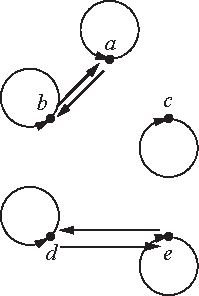
\includegraphics[width=\linewidth]{external/figps-exer73digraph.pdf}
\end{image}%
\tcblower
\end{figureptx}%
 Prove that \(\sim\) is an equivalence relation on the set \(A\), and determine all of the equivalence classes determined by this equivalence relation.%
\space\hyperlink{g:answer:idm818316040-back}{[Answer]}\end{divisionexercise}%
\begin{divisionexercise}{2}{}{}{x:exercise:exer_drawdirgraph}%
Let \(A = \left\{ a, b, c, d, e, f \right\}\), and assume that \(\sim\) is an equivalence relation on \(A\). Also assume that it is known that%
\begin{align*}
a \sim b \amp \amp a \not \sim c \amp \amp e \sim f\\
a \sim d \amp \amp a \not \sim f \amp \amp e \not \sim c
\end{align*}
Draw a complete directed graph for the equivalence relation \(\sim\) on the set \(A\), and then determine all of the equivalence classes for this equivalence relation.%
\space\hyperlink{g:answer:idm818308488-back}{[Answer]}\end{divisionexercise}%
\begin{divisionexercise}{3}{}{}{x:exercise:exer_sec73-2}%
Let \(A = \left\{ {0, 1, 2, 3, \ldots , 999, 1000} \right\}\). Define the relation \(R\) on \(A\) as follows: \begin{quote}%
For \(x, y \in A\), \(x \mathrel{R} y\) if and only if \(x\) and \(y\) have the same number of digits.\end{quote}
 Prove that \(R\) is an equivalence relation on the set \(A\) and determine all of the distinct equivalence classes determined by \(R\).%
\space\hyperlink{g:answer:idm818304392-back}{[Answer]}\end{divisionexercise}%
\begin{divisionexercise}{4}{}{}{x:exercise:exer_sec73-congclass}%
Determine all of the congruence classes for the relation of congruence modulo 5 on the set of integers.%
\space\hyperlink{g:answer:idm818286216-back}{[Answer]}\end{divisionexercise}%
\begin{divisionexercise}{5}{}{}{x:exercise:exer_modpowers}%
Let \(\Z_{9} = \left\{ 0, 1, 2, 3, 4, 5, 6, 7, 8 \right\}\).%
\begin{enumerate}[font=\bfseries,label=(\alph*),ref=\alph*]
\item{}Define the relation \(\sim\) on \(\Z_{9}\) as follows: For all \(a,
b \in \Z_{9}\), \(a \sim b\) if and only if \(a^2 \equiv b^2 \pmod {9}\). Prove that \(\sim\) is an equivalence relation on \(\Z_{9}\) and determine all of the distinct equivalence classes of this equivalence relation.%
\space\hyperlink{g:answer:idm818291848-back}{[Answer]}\item{}Define the relation \(\approx\) on \(\Z_{9}\) as follows: For all \(a,
b \in \Z_{9}\), \(a \approx b\) if and only if \(a^3 \equiv b^3 \pmod {9}\). Prove that \(\approx\) is an equivalence relation on \(\Z_{9}\) and determine all of the distinct equivalence classes of this equivalence relation.%
\end{enumerate}
\end{divisionexercise}%
\begin{divisionexercise}{6}{}{}{x:exercise:exer_sec73-integer}%
Define the relation \(\sim\) on \(\Q\) as follows: For \(a,
b \in \Q\), \(a \sim b\) if and only if \(a - b \in \Z\). In \hyperref[x:exercise:prog_example-equiv]{Progress Check~{\xreffont\ref{x:exercise:prog_example-equiv}}, p.\,\pageref{x:exercise:prog_example-equiv}} of \hyperref[x:section:S_equivrelations]{Section~{\xreffont\ref{x:section:S_equivrelations}}, p.\,\pageref{x:section:S_equivrelations}}, we showed that the relation \(\sim\) is an equivalence relation on \(\Q\). Also, see \hyperlink{x:exercise:exer_sec72-diffQ}{Exercise~{\xreffont 9}, p.\,\pageref{x:exercise:exer_sec72-diffQ}} in \hyperref[x:section:S_equivrelations]{Section~{\xreffont\ref{x:section:S_equivrelations}}, p.\,\pageref{x:section:S_equivrelations}}.%
\begin{enumerate}[font=\bfseries,label=(\alph*),ref=\alph*]
\item{}Prove that \(\left[ \dfrac{5}{7} \right] = \left\{ \left. m + \dfrac{5}{7} \right| m 
\in \Z \right\}\).%
\space\hyperlink{g:answer:idm818274312-back}{[Answer]}\item{}If \(a \in \Z\), then what is the equivalence class of \(a\)?%
\item{}If \(a \in \Z\), prove that there is a bijection from \(\left[ a \right]\) to \(\left[ \dfrac{5}{7} \right]\).%
\end{enumerate}
\end{divisionexercise}%
\begin{divisionexercise}{7}{}{}{x:exercise:exer_sec73-rationaldiff}%
Define the relation \(\sim\) on \(\R\) as follows: \begin{quote}%
For \(x,
y \in \R\), \(x \sim y\) if and only if \(x - y \in \Q\).\end{quote}
%
\begin{enumerate}[font=\bfseries,label=(\alph*),ref=\alph*]
\item{}Prove that \(\sim\) is an equivalence relation on \(\R\).%
\item{}List four different real numbers that are in the equivalence class of \(\sqrt{2}\).%
\item{}If \(a \in \Q\), what is the equivalence class of \(a\)?%
\item{}Prove that \(\left[ \sqrt{2} \right] = \left\{ r + \sqrt{2} \mid r \in \Q \right\}\).%
\item{}If \(a \in \Q\), prove that there is a bijection from \(\left[ a \right]\) to \(\left[ \sqrt{2} \right]\).%
\end{enumerate}
\end{divisionexercise}%
\begin{divisionexercise}{8}{}{}{g:exercise:idm818258568}%
Define the relation \(\sim\) on \(\Z\) as follows: For \(a,
b \in \Z\), \(a \sim b\) if and only if \(2a + 3b \equiv 0 \pmod 5\). The relation \(\sim\) is an equivalence relation on \(\Z\). (See \hyperlink{x:exercise:exer_modequivrel}{Exercise~{\xreffont 13}, p.\,\pageref{x:exercise:exer_modequivrel}} in \hyperref[x:section:S_equivrelations]{Section~{\xreffont\ref{x:section:S_equivrelations}}, p.\,\pageref{x:section:S_equivrelations}}). Determine all the distinct equivalence classes for this equivalence relation.%
\end{divisionexercise}%
\begin{divisionexercise}{9}{}{}{x:exercise:exer_sec73-rationals}%
Let \(A = \mathbb{Z} \times \left( {\mathbb{Z} - \left\{ 0 \right\}} \right)\). That is, \(A = \left\{ { {\left( {a, b} \right) \in \mathbb{Z} \times \mathbb{Z} } \mid b \ne 0} \right\}\). Define the relation \(\approx\) on \(A\) as follows: \begin{quote}%
For \(\left( {a, b} \right), \left( {c, d} \right) \in A\), \(\left( {a, b} \right) \approx \left( {c, d} \right)\) if and only if \(ad = bc\).\end{quote}
%
\begin{enumerate}[font=\bfseries,label=(\alph*),ref=\alph*]
\item{}Prove that \(\approx\) is an equivalence relation on \(A\).%
\space\hyperlink{g:answer:idm818004616-back}{[Answer]}\item{}Why was it necessary to include the restriction that \(b \ne 0\) in the definition of the set \(A\)?%
\item{}Determine an equation that gives a relation between \(a\) and \(b\) if \(\left( {a, b} \right) \in A\) and \(\left( {a, b} \right) \approx \left( {2, 3} \right)\).%
\space\hyperlink{g:answer:idm817994120-back}{[Answer]}\item{}Determine at least four different elements in \(\left[ {\left( {2, 3} \right)} \right]\), the equivalence class of \(\left( {2, 3} \right)\).%
\item{}Use set builder notation to describe \(\left[ {\left( {2, 3} \right)} \right]\), the equivalence class of \(\left( {2, 3} \right)\).%
\end{enumerate}
\end{divisionexercise}%
\begin{divisionexercise}{10}{}{}{g:exercise:idm817997064}%
For \(\left(a, b \right), \left( c, d \right) \in \R \times \R\), define \(\left(a, b \right) \sim \left(c, d \right)\) if and only if \(a^2 + b^2 = c^2 + d^2\). In \hyperlink{x:exercise:exer_sec72-circles}{Exercise~{\xreffont 15}, p.\,\pageref{x:exercise:exer_sec72-circles}} of \hyperref[x:section:S_equivrelations]{Section~{\xreffont\ref{x:section:S_equivrelations}}, p.\,\pageref{x:section:S_equivrelations}}, we proved that \(\sim\) is an equivalence relation on \(\R \times \R\).%
\begin{enumerate}[font=\bfseries,label=(\alph*),ref=\alph*]
\item{}Determine the equivalence class of \(\left(0, 0 \right)\).%
\item{}Use set builder notation (and do not use the symbol \(\sim\)) to describe the equivalence class of \(\left(2, 3 \right)\) and then give a geometric description of this equivalence class.%
\item{}Give a geometric description of a typical equivalence class for this equivalence relation.%
\item{}Let \(\R^* = \left\{ x \in \R \mid x \geq 0 \right\}\). Prove that there is a one-to-one correspondence (bijection) between \(\R^*\) and the set of all equivalence classes for this equivalence relation.%
\end{enumerate}
\end{divisionexercise}%
\begin{divisionexercise}{11}{}{}{g:exercise:idm817987080}%
Let \(A\) be a nonempty set and let \(\sim\) be an equivalence relation on \(A\). Prove each of the following:%
\begin{enumerate}[font=\bfseries,label=(\alph*),ref=\alph*]
\item{}For each \(a, b \in A\), \(a\nsim b\) if and only if \(\left[ a \right] \cap \left[ b \right] = \emptyset\).%
\item{}For each \(a,
b \in A\), if \(\left[ a \right] \ne \left[ b \right]\), then \(\left[ a \right] \cap \left[ b \right] = \emptyset\).%
\item{}For each \(a, b \in A\), if \(\left[ a \right] \cap \left[ b \right] \ne \emptyset\) then \(\left[ a \right] = \left[ b \right]\).%
\end{enumerate}
\end{divisionexercise}%
\begin{activity}{A Partition Defines an Equivalence Relation.}{x:activity:exer_partition-equivrelation}%
Let \(A = \left\{ {a, b, c, d, e} \right\}\) and let \(\mathcal{C} = 
\left\{ {\left\{ {a, b, c} \right\}, \left\{ {d, e} \right\}} \right\}\).%
\begin{enumerate}[font=\bfseries,label=(\alph*),ref=\alph*]
\item{}Explain why \(\mathcal{C}\) is a partition of \(A\).%
\item\label{x:task:A_partition-equivrelation1}Define a relation \(\sim\) on \(A\) as follows: For \(x, y \in A\), \(x \sim y\) if and only if there exists a set \(U\) in \(\mathcal{C}\) such that \(x \in U\) and \(y \in U\).%
\par
Prove that \(\sim\) is an equivalence relation on the set \(A\), and then determine all the equivalence classes for \(\sim\). How does the collection of all equivalence classes compare to \(\mathcal{C}\)?%
\item{}What we did for the specific partition in \hyperref[x:task:A_partition-equivrelation1]{Task~{\xreffont\ref{x:activity:exer_partition-equivrelation}}.{\xreffont\ref{x:task:A_partition-equivrelation1}}, p.\,\pageref{x:task:A_partition-equivrelation1}} can be done for any partition of a set. So to generalize \hyperref[x:task:A_partition-equivrelation1]{Task~{\xreffont\ref{x:activity:exer_partition-equivrelation}}.{\xreffont\ref{x:task:A_partition-equivrelation1}}, p.\,\pageref{x:task:A_partition-equivrelation1}}, we let \(A\) be a nonempty set and let \(\mathcal{C}\) be a partition of \(A\). We then define a relation \(\sim\) on \(A\) as follows: \begin{quote}%
For \(x, y \in A\), \(x \sim y\) if and only if there exists a set \(U\) in \(\mathcal{C}\) such that \(x \in U\) and \(y \in U\).\end{quote}
%
\par
Prove that \(\sim\) is an equivalence relation on the set \(A\).%
\item{}Let \(a \in A\) and let \(U \in \mathcal{C}\) such that \(a \in U\). Prove that \([ a ] = U\).%
\end{enumerate}
\end{activity}%
\begin{activity}{Equivalence Relations on a Set of Matrices.}{g:activity:idm817963912}%
The following exercises require a knowledge of elementary linear algebra. We let \(\mathcal{M}_{n, n}\left( \R \right)\) be the set of all \(n\) by \(n\) matrices with real number entries.%
\begin{enumerate}[font=\bfseries,label=(\alph*),ref=\alph*]
\item{}Define a relation \(\sim\) on \(\mathcal{M}_{n, n}( \R )\) as follows: For all \(A, B \in \mathcal{M}_{n, n}( \R )\), \(A \sim B\) if and only if there exists an invertible matrix \(P\) in \(\mathcal{M}_{n, n}( \R )\) such that \(B = PAP^{-1}\). Is \(\sim\) an equivalence relation on \(\mathcal{M}_{n, n}( \R )\)? Justify your conclusion.%
\item{}Define a relation \(R\) on \(\mathcal{M}_{n, n} (\R )\) as follows: For all \(A, B \in \mathcal{M}_{n, n}( \R )\), \(A \mathrel{R} B\) if and only if \(\text{ det } (A) = \text{ det } (B)\). Is \(R\) an equivalence relation on \(\mathcal{M}_{n, n}( \R )\)? Justify your conclusion.%
\item{}Let \(\sim\) be an equivalence relation on \(\R\). Define a relation \(\approx\) on \(\mathcal{M}_{n, n}( \R )\) as follows: For all \(A, B \in \mathcal{M}_{n, n}( \R )\), \(A \approx B\) if and only if \(\text{ det } (A) \sim \text{ det } (B)\). Is \(\approx\) an equivalence relation on \(\mathcal{M}_{n, n}( \R )\)? Justify your conclusion.%
\end{enumerate}
\end{activity}%
\end{exercises-subsection}
\end{sectionptx}
%
%
\typeout{************************************************}
\typeout{Section 7.4 Modular Arithmetic}
\typeout{************************************************}
%
\begin{sectionptx}{Modular Arithmetic}{}{Modular Arithmetic}{}{}{x:section:S_modulararithmetic}
%
%
\typeout{************************************************}
\typeout{Beginning Activity  Beginning Activity 1: Congruence Modulo 6}
\typeout{************************************************}
%
\begin{worksheet-subsection}{Beginning Activity 1: Congruence Modulo 6}{}{Beginning Activity 1: Congruence Modulo 6}{}{}{x:worksheet:PA_congruencemod6}
For this activity, we will only use the relation of congruence modulo 6 on the set of integers.%
\begin{divisionexercise}{1}{}{}{x:exercise:PA_congruencemod6-1}%
Find five different integers \(a\) such that \(a \equiv 3 \pmod 6\) and find five different integers \(b\) such that \(b \equiv 4 \pmod 6\). That is, find five different integers in \([3]\), the congruence class of 3 modulo 6 and five different integers in \([4]\), the congruence class of 4 modulo 6.%
\end{divisionexercise}%
\begin{divisionexercise}{2}{}{}{g:exercise:idm817944712}%
Calculate \(s = a + b\) using several values of \(a\) in \([3]\) and several values of \(b\) in \([4]\) from \hyperlink{x:exercise:PA_congruencemod6-1}{Exercise~{\xreffont 1}, p.\,\pageref{x:exercise:PA_congruencemod6-1}}. For each sum \(s\) that is calculated, find \(r\) so that \(0 \leq r \lt 6\) and \(s \equiv r \pmod 6\). What do you observe?%
\end{divisionexercise}%
\begin{divisionexercise}{3}{}{}{g:exercise:idm817946120}%
Calculate \(p = a \cdot b\) using several values of \(a\) in \([3]\) and several values of \(b\) in \([4]\) from \hyperlink{x:exercise:PA_congruencemod6-1}{Exercise~{\xreffont 1}, p.\,\pageref{x:exercise:PA_congruencemod6-1}}. For each product \(p\) that is calculated, find \(r\) so that \(0 \leq r \lt 6\) and \(p \equiv r \pmod 6\). What do you observe?%
\end{divisionexercise}%
\begin{divisionexercise}{4}{}{}{g:exercise:idm817937160}%
Calculate \(q = a^2\) using several values of \(a\) in \([3]\) from \hyperlink{x:exercise:PA_congruencemod6-1}{Exercise~{\xreffont 1}, p.\,\pageref{x:exercise:PA_congruencemod6-1}}. For each product \(q\) that is calculated, find \(r\) so that \(0 \leq r \lt 6\) and \(q \equiv r \pmod 6\). What do you observe?%
\end{divisionexercise}%
\end{worksheet-subsection}
%
%
\typeout{************************************************}
\typeout{Beginning Activity  Beginning Activity 2: The Remainder When Dividing by 9}
\typeout{************************************************}
%
\begin{worksheet-subsection}{Beginning Activity 2: The Remainder When Dividing by 9}{}{Beginning Activity 2: The Remainder When Dividing by 9}{}{}{x:worksheet:PA_remainderdivide9}
If \(a\) and \(b\) are integers with \(b > 0\), then from the Division Algorithm, we know that there exist unique integers \(q\) and \(r\) such that%
\begin{equation*}
a = bq + r \text{ and }  0 \leq r \lt  b\text{.}
\end{equation*}
In this activity, we are interested in the remainder \(r\). Notice that \(r = a - bq\). So, given \(a\) and \(b\), if we can calculate \(q\), then we can calculate \(r\).%
\par
We can use the ``int'' function on a calculator to calculate \(q\). [The ``int'' function is the ``greatest integer function.'' If \(x\) is a real number, then \(\operatorname{int}( x )\) is the greatest integer that is less than or equal to \(x\).]%
\par
So, in the context of the Division Algorithm, \(q = \operatorname{int} \!\left( {\dfrac{a}{b}} \right)\). Consequently,%
\begin{equation*}
r = a - b \cdot \operatorname{int} \!\left( {\frac{a}{b}} \right)\text{.}
\end{equation*}
If \(n\) is a positive integer, we will let \(s\left( n \right)\) denote the sum of the digits of \(n\). For example, if \(n = 731\), then%
\begin{equation*}
s( {731} ) = 7 + 3 + 1 = 11\text{.}
\end{equation*}
%
\par
For each of the following values of \(n\), calculate%
\begin{itemize}[label=\textbullet]
\item{}The remainder when \(n\) is divided by 9, and%
\item{}The value of \(s( n )\) and the remainder when \(s( n )\) is divided by 9.%
\end{itemize}
%
\begin{divisionexercise}{1}{}{}{g:exercise:idm817917192}%
\(n=498\)%
\end{divisionexercise}%
\begin{divisionexercise}{2}{}{}{g:exercise:idm817923720}%
\(n=7319\)%
\end{divisionexercise}%
\begin{divisionexercise}{3}{}{}{g:exercise:idm817916296}%
\(n=4672\)%
\end{divisionexercise}%
\begin{divisionexercise}{4}{}{}{g:exercise:idm817915912}%
\(n=9845\)%
\end{divisionexercise}%
\begin{divisionexercise}{5}{}{}{g:exercise:idm817911944}%
\(n=51381\)%
\end{divisionexercise}%
\begin{divisionexercise}{6}{}{}{g:exercise:idm817913864}%
\(n=305877\)%
\end{divisionexercise}%
\begin{conclusion}{}%
What do you observe?%
\end{conclusion}%
\end{worksheet-subsection}
%
%
\typeout{************************************************}
\typeout{Subsection  The Integers Modulo \(\boldsymbol{n}\)}
\typeout{************************************************}
%
\begin{subsectionptx}{The Integers Modulo \(\boldsymbol{n}\)}{}{The Integers Modulo \(\boldsymbol{n}\)}{}{}{g:subsection:idm817915144}
Let \(n \in \mathbb{N}\). Since the relation of congruence modulo \(n\) is an equivalence relation on \(\mathbb{Z}\), we can discuss its equivalence classes. Recall that in this situation, we refer to the equivalence classes as congruence classes.%
\begin{assemblage}{Definition.}{x:assemblage:integersmodn}%
\label{g:notation:idm817912200} Let \(n \in \mathbb{N}\). The set of congruence classes for the relation of congruence modulo \(n\) on \(\mathbb{Z}\) is the set of \terminology{integers modulo \(\boldsymbol{n}\)}, or the set of integers mod \(n\). We will denote this set of congruence classes by \(\mathbb{Z}_{n}\).%
\end{assemblage}
\hyperref[x:corollary:C_propsofcongclasses2]{Corollary~{\xreffont\ref{x:corollary:C_propsofcongclasses2}}, p.\,\pageref{x:corollary:C_propsofcongclasses2}} tells us that%
\begin{equation*}
\mathbb{Z} = [ 0 ] \cup [ 1 ] \cup [ 2 ] \cup   \cdots  \cup  [ {n - 1} ]\text{.}
\end{equation*}
In addition, we know that each integer is congruent to precisely one of the integers \(0, 1, 2, \ldots , n - 1\). This tells us that one way to represent \(\mathbb{Z}_{n}\) is%
\begin{equation*}
\mathbb{Z}_{n}  = \left\{ {[ 0 ], [ 1 ], [ 2 ],  \ldots, [ {n - 1} ]} \right\}\text{.}
\end{equation*}
Consequently, even though each integer has a congruence class, the set \(\mathbb{Z}_{n}\) has only \(n\) distinct congruence classes.%
\par
The set of integers \(\Z\) is more than a set. We can add and multiply integers. That is, there are the arithmetic operations of addition and multiplication on the set \(\Z\), and we know that \(\Z\) is closed with respect to these two operations.%
\par
One of the basic problems dealt with in modern algebra is to determine if the arithmetic operations on one set ``transfer'' to a related set. In this case, the related set is \(\mathbb{Z}_{n}\). For example, in the integers modulo 5, \(\Z_5\), is it possible to add the congruence classes \([ 4 ]\) and \([ 2 ]\) as follows?%
\begin{align*}
\oplus [ 2 ] \amp = [ {4 + 2} ]\\
\amp = [ 6 ]\\
\amp = [ 1 ]\text{.}
\end{align*}
%
\par
We have used the symbol \(\oplus\) to denote addition in \(\mathbb{Z}_{5}\) so that we do not confuse it with addition in \(\mathbb{Z}\). This looks simple enough, but there is a problem. The congruence classes \([ 4 ]\) and \([ 2 ]\) are not numbers, \emph{they are infinite sets}. We have to make sure that we get the same answer no matter what element of \([ 4 ]\) we use and no matter what element of \([ 2 ]\) we use. For example,%
\begin{align*}
9 \amp \equiv 4 \pmod 5  \amp \amp \text{ and so } \amp \amp [ 9 ] = [ 4 ].  \text{  Also, }\\
7 \amp \equiv 2 \pmod 5  \amp \amp \text{ and so } \amp \amp [ 7 ] = [ 2 ]\text{.}
\end{align*}
Do we get the same result if we add \([ 9 ]\) and \([ 7 ]\) in the way we did when we added \([ 4 ]\) and \([ 2 ]\)? The following computation confirms that we do:%
\begin{align*}
\oplus [ 7 ] \amp = [ {9 + 7} ]\\
\amp = [ {16} ]\\
\amp = [ 1 ]\text{.}
\end{align*}
%
\par
This is one of the ideas that was explored in \hyperref[x:worksheet:PA_congruencemod6]{Beginning Activity 1, p.\,\pageref{x:worksheet:PA_congruencemod6}}. The main difference is that in this activity, we used the relation of congruence, and here we are using congruence classes. All of the examples in \hyperref[x:worksheet:PA_congruencemod6]{Beginning Activity 1, p.\,\pageref{x:worksheet:PA_congruencemod6}} should have illustrated the properties of congruence modulo 6 in the following table. The left side shows the properties in terms of the congruence relation and the right side shows the properties in terms of the congruence classes.%
\begin{sidebyside}{2}{0}{0}{0}%
\begin{sbspanel}{0.5}%
If \(a \equiv 3 \pmod 6\) and  \(b \equiv 4 \pmod 6\), then%
\begin{itemize}[label=\textbullet]
\item{}\(\left( {a + b} \right) \equiv \left( {3 + 4} \right) \pmod 6\);%
\item{}\(\left( {a \cdot b} \right) \equiv \left( {3 \cdot 4} \right) \pmod 6\).%
\end{itemize}
%
\end{sbspanel}%
\begin{sbspanel}{0.5}%
\par
If \([ a ] = [ 3 ]\)  and  \([ b ] = [ 4 ]\) in \(\Z_6\), then%
\begin{itemize}[label=\textbullet]
\item{}\([ {a + b} ] = [ {3 + 4} ]\);%
\item{}\([ {a \cdot b} ] = [ {3 \cdot 4} ]\).%
\end{itemize}
%
\end{sbspanel}%
\end{sidebyside}%
\par
These are illustrations of general properties that we have already proved in \hyperref[x:theorem:T_propsofcong]{Theorem~{\xreffont\ref{x:theorem:T_propsofcong}}, p.\,\pageref{x:theorem:T_propsofcong}}. We repeat the statement of the theorem here because it is so important for defining the operations of addition and multiplication in \(\mathbb{Z}_{n}\).%
\begin{paragraphs}{Theorem~{\xreffont\ref*{x:theorem:T_propsofcong}} Restated.}{g:paragraphs:idm817877128}%
Let \(n\) be a natural number and let \(a,
b, c, \text{ and } d\) be integers. Then%
\begin{enumerate}
\item{}If \(a \equiv b \pmod n\) and \(c \equiv d \pmod n\), then \(\left( {a + c} \right) \equiv \left( {b + d} \right) \pmod n\).%
\item{}If \(a \equiv b \pmod n\) and \(c \equiv d \pmod n\), then \(ac \equiv bd \pmod n\).%
\item{}If \(a \equiv b \pmod n\) and \(m \in \mathbb{N}\), then \(a^m \equiv b^m \pmod n\).%
\end{enumerate}
%
\end{paragraphs}%
\par
Since \(x \equiv y \pmod n\) if and only if \([ x ] = [ y ]\), we can restate the result of this \hyperref[x:theorem:T_propsofcong]{Theorem~{\xreffont\ref{x:theorem:T_propsofcong}}, p.\,\pageref{x:theorem:T_propsofcong}} in terms of congruence classes in \(\mathbb{Z}_n\).%
\begin{corollary}{}{}{x:corollary:C_propsofcong-76}%
Let \(n\) be a natural number and let \(a,
b, c\), and \(d\) be integers. Then, in \(\mathbb{Z}_n\),%
\begin{enumerate}
\item{}If \([ a ] = [ b ]\) and \([ c ] = [ d ]\), then \([ {a + c} ] = [ {b + d} ]\).%
\item{}If \([ a ] = [ b ]\) and \([ c ] = [ d ]\), then \([ {a \cdot c} ] = [ {b \cdot d} ]\).%
\item{}If \([ a ] = [ b ]\) and \(m \in \mathbb{N}\), then \([ a ^m] = [ b ^m]\).%
\end{enumerate}
%
\end{corollary}
Because of \hyperref[x:corollary:C_propsofcong-76]{Corollary~{\xreffont\ref{x:corollary:C_propsofcong-76}}, p.\,\pageref{x:corollary:C_propsofcong-76}}, we know that the following formal definition of addition and multiplication of congruence classes in \(\mathbb{Z}_{n}\) is independent of the choice of the elements we choose from each class. We say that these definitions of addition and multiplication are \terminology{well defined}.%
\begin{assemblage}{Definition.}{x:assemblage:modulararithmetic}%
\label{g:notation:idm817860872}\label{g:notation:idm817864200} Let \(n \in \mathbb{N}\). \terminology{Addition and multiplication} in \(\mathbb{Z}_n\) are defined as follows: For \([ a ], [ c ] \in \mathbb{Z}_n\),%
\begin{equation*}
[ a ] \oplus [ c ] = [ {a + c} ] \text{  and  } [ a ] \odot [ c ] = [ {ac} ]\text{.}
\end{equation*}
%
\par
The term \terminology{modular arithmetic} is used to refer to the operations of addition and multiplication of congruence classes in the integers modulo~\(n\).%
\end{assemblage}
So if \(n \in \mathbb{N}\), then we have an addition and multiplication defined on \(\mathbb{Z}_n\), the integers modulo~\(n\).%
\par
Always remember that for each of the equations in the definitions, the operations on the left, \(\oplus \text{ and } \odot\), are the new operations that are being defined. The operations on the right side of the equations \(\left( + \text{ and } \cdot \right)\) are the known operations of addition and multiplication in \(\mathbb{Z}\).%
\par
Since \(\mathbb{Z}_n\) is a finite set, it is possible to construct addition and multiplication tables for \(\mathbb{Z}_n\). In constructing these tables, we follow the convention that all sums and products should be in the form \([ r]\), where \(0 \leq r \lt  n\). For example, in \(\Z_3\), we see that by the definition, \([1] \oplus [2] = [3]\), but since \(3 \equiv 0 \pmod 3\), we see that \([3] = [0]\) and so we write%
\begin{equation*}
[1] \oplus [2] = [3] = [0]\text{.}
\end{equation*}
Similarly, by definition, \([2] \odot [2] = [4]\), and in \(\Z_3\), \([4] = [1]\). So we write%
\begin{equation*}
[2] \odot [2] = [4] = [1]\text{.}
\end{equation*}
The complete addition and multiplication tables for \(\Z_3\) are%
\begin{sidebyside}{2}{0.1}{0.1}{0.2}%
\begin{sbspanel}{0.3}%
\resizebox{\ifdim\width > \linewidth\linewidth\else\width\fi}{!}{%
{\centering%
{\tabularfont%
\begin{tabular}{cccc}
\multicolumn{1}{cB}{\(\oplus\)}&\([ 0 ]\)&\([ 1 ]\)&\([2]\)\tabularnewline\hrulemedium
\multicolumn{1}{cB}{\([ 0 ]\)}&\([ 0 ]\)&\([ 1 ]\)&\([2]\)\tabularnewline[0pt]
\multicolumn{1}{cB}{\([ 1 ]\)}&\([ 1 ]\)&\([ 2 ]\)&\([0]\)\tabularnewline[0pt]
\multicolumn{1}{cB}{\([ 2 ]\)}&\([ 2 ]\)&\([ 0 ]\)&\([1]\)
\end{tabular}
}%
\par}
}%
\end{sbspanel}%
\begin{sbspanel}{0.3}%
\resizebox{\ifdim\width > \linewidth\linewidth\else\width\fi}{!}{%
{\centering%
{\tabularfont%
\begin{tabular}{cccc}
\multicolumn{1}{cB}{\(\odot\)}&\([ 0 ]\)&\([ 1 ]\)&\([2]\)\tabularnewline\hrulemedium
\multicolumn{1}{cB}{\([ 0 ]\)}&\([ 0 ]\)&\([ 0 ]\)&\([0]\)\tabularnewline[0pt]
\multicolumn{1}{cB}{\([ 1 ]\)}&\([ 0 ]\)&\([ 1 ]\)&\([2]\)\tabularnewline[0pt]
\multicolumn{1}{cB}{\([ 2 ]\)}&\([ 0 ]\)&\([ 2 ]\)&\([1]\)
\end{tabular}
}%
\par}
}%
\end{sbspanel}%
\end{sidebyside}%
\begin{inlineexercise}{Modular Arithmetic in \(\boldsymbol{\Z_2}\), \(\boldsymbol{\Z_5}\), and \(\boldsymbol{\Z_6}\).}{x:exercise:prog_modulararithmetic5-6}%
\begin{enumerate}[font=\bfseries,label=(\alph*),ref=\alph*]
\item{}Construct addition and multiplication tables for \(\Z_2\), the integers modulo 2.%
\space\hyperlink{g:solution:idm817826312-back}{[Solution]}\item\label{x:task:exam_sec74-tables}Verify that the following addition and multiplication tables for \(\mathbb{Z}_5\) are correct. \begin{sidebyside}{2}{0.025}{0.025}{0.05}%
\begin{sbspanel}{0.45}%
\resizebox{\ifdim\width > \linewidth\linewidth\else\width\fi}{!}{%
{\centering%
{\tabularfont%
\begin{tabular}{cccccc}
\multicolumn{1}{cB}{\(\oplus\)}&\([ 0 ]\)&\([ 1 ]\)&\([ 2 ]\)&\([ 3 ]\)&\([ 4 ]\)\tabularnewline\hrulemedium
\multicolumn{1}{cB}{\([ 0 ]\)}&\([ 0 ]\)&\([ 1 ]\)&\([ 2 ]\)&\([ 3 ]\)&\([ 4 ]\)\tabularnewline[0pt]
\multicolumn{1}{cB}{\([ 1 ]\)}&\([ 1 ]\)&\([ 2 ]\)&\([ 3 ]\)&\([ 4 ]\)&\([ 0 ]\)\tabularnewline[0pt]
\multicolumn{1}{cB}{\([ 2 ]\)}&\([ 2 ]\)&\([ 3 ]\)&\([ 4 ]\)&\([ 0 ]\)&\([ 1 ]\)\tabularnewline[0pt]
\multicolumn{1}{cB}{\([ 3 ]\)}&\([ 3 ]\)&\([ 4 ]\)&\([ 0 ]\)&\([ 1 ]\)&\([ 2 ]\)\tabularnewline[0pt]
\multicolumn{1}{cB}{\([ 4 ]\)}&\([ 4 ]\)&\([ 0 ]\)&\([ 1 ]\)&\([ 2 ]\)&\([ 3 ]\)
\end{tabular}
}%
\par}
}%
\end{sbspanel}%
\begin{sbspanel}{0.45}%
\resizebox{\ifdim\width > \linewidth\linewidth\else\width\fi}{!}{%
{\centering%
{\tabularfont%
\begin{tabular}{cccccc}
\multicolumn{1}{cB}{\(\odot\)}&\([ 0 ]\)&\([ 1 ]\)&\([ 2 ]\)&\([ 3 ]\)&\([ 4 ]\)\tabularnewline\hrulemedium
\multicolumn{1}{cB}{\([ 0 ]\)}&\([ 0 ]\)&\([ 0 ]\)&\([ 0 ]\)&\([ 0 ]\)&\([ 0 ]\)\tabularnewline[0pt]
\multicolumn{1}{cB}{\([ 1 ]\)}&\([ 0 ]\)&\([ 1 ]\)&\([ 2 ]\)&\([ 3 ]\)&\([ 4 ]\)\tabularnewline[0pt]
\multicolumn{1}{cB}{\([ 2 ]\)}&\([ 0 ]\)&\([ 2 ]\)&\([ 4 ]\)&\([ 1 ]\)&\([ 3 ]\)\tabularnewline[0pt]
\multicolumn{1}{cB}{\([ 3 ]\)}&\([ 0 ]\)&\([ 3 ]\)&\([ 1 ]\)&\([ 4 ]\)&\([ 2 ]\)\tabularnewline[0pt]
\multicolumn{1}{cB}{\([ 4 ]\)}&\([ 0 ]\)&\([ 4 ]\)&\([ 3 ]\)&\([ 2 ]\)&\([ 1 ]\)
\end{tabular}
}%
\par}
}%
\end{sbspanel}%
\end{sidebyside}%
%
\item{}Construct complete addition and multiplication tables for \(\Z_6\).%
\space\hyperlink{g:solution:idm817780488-back}{[Solution]}\item{}In the integers, the following statement is true. We sometimes call this the zero product property for the integers. \begin{quote}%
For all \(a, b \in \Z\), if \(a \cdot b = 0\), then \(a = 0\) or \(b = 0\).\end{quote}
 Write the contrapositive of the conditional statement in this property.%
\space\hyperlink{g:solution:idm817536408-back}{[Solution]}\item{}Are the following statements true or false? Justify your conclusions.%
\begin{enumerate}[font=\bfseries,label=(\roman*),ref=\theenumi.\roman*]
\item{}For all \([ a ], [ b ] \in \Z_5\), if \([ a ] \odot [ b ] = [ 0 ]\), then \([ a ] = [ 0 ]\) or \([ b ] = [ 0 ]\).%
\space\hyperlink{g:solution:idm817535000-back}{[Solution]}\item{}For all \([ a ], [ b ] \in \Z_6\), if \([ a ] \odot [ b ] = [ 0 ]\), then \([ a ] = [ 0 ]\) or \([ b ] = [ 0 ]\).%
\space\hyperlink{g:solution:idm817531160-back}{[Solution]}\end{enumerate}
\end{enumerate}
\end{inlineexercise}%
\end{subsectionptx}
%
%
\typeout{************************************************}
\typeout{Subsection  Divisibility Tests}
\typeout{************************************************}
%
\begin{subsectionptx}{Divisibility Tests}{}{Divisibility Tests}{}{}{g:subsection:idm817523736}
Congruence arithmetic can be used to prove certain divisibility tests. For example, you may have learned that a natural number is divisible by 9 if the sum of its digits is divisible by 9. As an easy example, note that the sum of the digits of 5823 is equal to \(5 + 8 + 2 + 3 = 18\), and we know that 18 is divisible by 9. It can also be verified that 5823 is divisible by 9. (The quotient is 647.) We can actually generalize this property by dealing with remainders when a natural number is divided by 9.%
\par
Let \(n \in \mathbb{N}\) and let \(s( n )\) denote the sum of the digits of \(n\). For example, if \(n = 7319\), then \(s( {7319} ) = 7 + 3 + 1 + 9 = 20\). In \hyperref[x:worksheet:PA_remainderdivide9]{Beginning Activity 2, p.\,\pageref{x:worksheet:PA_remainderdivide9}}, we saw that%
\begin{equation*}
7319 \equiv 2 \pmod 9 \text{ and } 20 \equiv 2 \pmod 9\text{.}
\end{equation*}
In fact, for every example in \hyperref[x:worksheet:PA_remainderdivide9]{Beginning Activity 2, p.\,\pageref{x:worksheet:PA_remainderdivide9}}, we saw that \(n\) and \(s( n )\) were congruent modulo 9 since they both had the same remainder when divided by 9. The concepts of congruence and congruence classes can help prove that this is always true.%
\par
We will use the case of \(n = 7319\) to illustrate the general process. We must use our standard place value system. By this, we mean that we will write \(7319\) as follows:%
\begin{equation}
7319 = \left( {7 \times 10^3 } \right) + \left( {3 \times 10^2 } \right) + \left( {1 
\times 10^1 } \right) + \left( 9 \times 10^0 \right)\text{.}\label{x:men:eq_divideby9-1}
\end{equation}
%
\par
The idea is to now use the definition of addition and multiplication in \(\mathbb{Z}_9\) to convert equation (1) to an equation in \(\mathbb{Z}_9\). We do this as follows:%
\begin{align}
\amp = [ {\left( {7 \times 10^3 } \right) + \left( {3 \times 10^2 }  
\right) + \left( {1 \times 10^1 } \right) + \left( 9 \times 10^0 \right)} ]\notag\\
\amp = [ {7 \times 10^3 } ] \oplus [ {3 \times 10^2 } ]  
\oplus [ {1 \times 10^1 } ] \oplus [ {9 \times 10^0 } ]\notag\\
\amp = \left( {[ 7 ] \odot [ {10^3 } ]} \right) 
\oplus \left( {[ 3 ] \odot [ {10}^2 ]} \right) \oplus \left( {[ 1 ] \odot [ 10^ 1 ]} 
\right) \oplus \left( [ 9 ] \odot [ 1 ] \right)\label{x:mrow:eq_divideby9-2}
\end{align}
%
\par
Since \(10^3  \equiv 1 \pmod 9\), \(10^2  \equiv 1 \pmod 9\) and \(10 \equiv 1 \pmod 9\), we can conclude that \([ 10^3 ] = [ 1 ]\), \([ {10^2 } ] = [ 1 ]\) and \([ {10} ] = [ 1 ]\). Hence, we can use these facts and equation \hyperref[x:mrow:eq_divideby9-2]{({\xreffont\ref{x:mrow:eq_divideby9-2}})} to obtain%
\begin{align}
[ {7319} ] \amp =\left( {[ 7 ] \odot [ {10^3 } ]} \right) \oplus 
\left( {[ 3 ] \odot [ {10^2} ]} \right) \oplus \left( {[ 1 ] \odot [ 10 ]} \right) 
\oplus \left( [ 9 ] \odot [ 1 ] \right)\notag\\
\amp = \left( {[ 7 ] \odot [ 1 ]} \right) \oplus \left( {[ 3 ] 
\odot [ 1 ]} \right) \oplus \left( {[ 1 ] \odot [ 1 ]} \right) \oplus \left( [ 9 ] 
\odot [ 1 ] \right)\notag\\
\amp = [ 7 ] \oplus [ 3 ] \oplus [ 1 ] \oplus [ 9 ]\notag\\
\amp = [ {7 + 3 + 1 + 9} ]\label{x:mrow:eq_divideby9-3}
\end{align}
Equation \hyperref[x:mrow:eq_divideby9-3]{({\xreffont\ref{x:mrow:eq_divideby9-3}})} tells us that 7319 has the same remainder when divided by 9 as the sum of its digits. It is easy to check that the sum of the digits is 20 and hence has a remainder of 2. This means that when 7319 is divided by 9, the remainder is 2.%
\par
To prove that any natural number has the same remainder when divided by 9 as the sum of its digits, it is helpful to introduce notation for the decimal representation of a natural number. The notation we will use is similar to the notation for the number 7319 in equation \hyperref[x:men:eq_divideby9-1]{({\xreffont\ref{x:men:eq_divideby9-1}})}.%
\par
In general, if \(n \in \mathbb{N}\), and \(n = a_k a_{k - 1} \cdots a_1 a_0\) is the decimal representation of \(n\), then%
\begin{equation*}
n = \left( {a_k  \times 10^k } \right) + \left( {a_{k - 1}  \times 10^{k - 1} } \right) + 
\cdots  + \left( {a_1  \times 10^1 } \right) + \left( {a_0  \times 10^0 } \right)\!\text{.}
\end{equation*}
This can also be written using summation notation as follows:%
\begin{equation*}
n = \sum\limits_{j = 0}^k {\left( {a_j  \times 10^j } \right)}\text{.}
\end{equation*}
%
\par
Using congruence classes for congruence modulo 9, we have%
\begin{align}
\amp = [ {\left( {a_k  \times 10^k } \right) + \left( {a_{k - 1}  
\times 10^{k - 1} } \right) +  \cdots  + \left( {a_1  \times 10^1 } \right) + 
\left( {a_0  \times 10^0 } \right)} ]\notag\\
\amp = [ {a_k  \times 10^k } ] \oplus [ {a_{k - 1}  
\times 10^{k - 1} } ] \oplus  \cdots  \oplus [ {a_1  \times 10^1 } ] 
\oplus [ {a_0  \times 10^0 } ]\notag\\
\amp = \left( {[ {a_k } ] \odot [ {10^k } ]} \right) 
\oplus \left( {[ {a_{k - 1} } ] \odot [ {10^{k - 1} } ]} \right) \oplus \cdots\notag\\
\amp  \hspace{5cm} \oplus \left( {[ {a_1 } ] 
\odot [ {10^1 } ]} \right) \oplus \left( {[ {a_0 } ] \odot [ {10^0 } ]} \right)\!\label{x:mrow:eq_divideby9-4}
\end{align}
%
\par
One last detail is needed. It is given in \hyperref[x:proposition:P_poweroftenmod9]{Proposition~{\xreffont\ref{x:proposition:P_poweroftenmod9}}, p.\,\pageref{x:proposition:P_poweroftenmod9}}. The proof by mathematical induction is \hyperlink{x:exercise:exer_poweroftenmod9}{Exercise~{\xreffont 6}, p.\,\pageref{x:exercise:exer_poweroftenmod9}}.%
\begin{proposition}{}{}{x:proposition:P_poweroftenmod9}%
If \(n\) is a nonnegative integer, then \(10^n \equiv 1 \pmod 9\), and hence for the equivalence relation of congruence modulo 9, \([ {10^n } ] = [ 1 ]\).%
\end{proposition}
If we let \(s( n )\) denote the sum of the digits of \(n\), then%
\begin{equation*}
s( n ) = a_k  + a_{k - 1}  +  \cdots  + a_1  + a_0\text{,}
\end{equation*}
%
\par
Now using equation \hyperref[x:mrow:eq_divideby9-4]{({\xreffont\ref{x:mrow:eq_divideby9-4}})} and \hyperref[x:proposition:P_poweroftenmod9]{Proposition~{\xreffont\ref{x:proposition:P_poweroftenmod9}}, p.\,\pageref{x:proposition:P_poweroftenmod9}}, we obtain%
\begin{align*}
[ n ] \amp = \left( {[ {a_k } ] \odot [ 1 ]} \right) \oplus 
\left( {[ {a_{k - 1} } ] \odot [ 1 ]} \right) \oplus  \cdots  \oplus \left( {[ {a_1 } ] 
\odot [ 1 ]} \right) \oplus \left( {[ {a_0 } ] \odot [ 1 ]} \right)\\
\amp = [ {a_k } ] \oplus [ {a_{k - 1} } ] \oplus  \cdots  \oplus [ {a_1 } ] 
\oplus [ {a_0 } ]\\
\amp = [ {a_k  + a_{k - 1}  +  \cdots  + a_1  + a_0 } ].\\
\amp = [ s( n ) ]\text{.}
\end{align*}
This completes the proof of \hyperref[x:theorem:T_sumofdigitsmod9]{Theorem~{\xreffont\ref{x:theorem:T_sumofdigitsmod9}}, p.\,\pageref{x:theorem:T_sumofdigitsmod9}}.%
\begin{theorem}{}{}{x:theorem:T_sumofdigitsmod9}%
Let \(n \in \mathbb{N}\) and let \(s( n )\) denote the sum of the digits of \(n\). Then%
\begin{enumerate}
\item{}\([ n ] = [ {s( n )} ]\), using congruence classes modulo 9.%
\item{}\(n \equiv s( n ) \pmod 9\).%
\item\label{x:li:T_sumofdigitsmod9-part}{}\hypertarget{x:li:T_sumofdigitsmod9-part}{}\(9 \mid n\) if and only if \(9 \mid s( n )\).%
\end{enumerate}
%
\end{theorem}
\index{divisibility test}\index{divisibility test!for 9} \hyperlink{x:li:T_sumofdigitsmod9-part}{Item~{\xreffont 3}, p.\,\pageref{x:li:T_sumofdigitsmod9-part}} of \hyperref[x:theorem:T_sumofdigitsmod9]{Theorem~{\xreffont\ref{x:theorem:T_sumofdigitsmod9}}, p.\,\pageref{x:theorem:T_sumofdigitsmod9}} is called a \terminology{divisibility test}. If gives a necessary and sufficient condition for a natural number to be divisible by 9. Other divisibility tests will be explored in the exercises. Most of these divisibility tests can be proved in a manner similar to the proof of the divisibility test for 9.%
\end{subsectionptx}
%
%
\typeout{************************************************}
\typeout{Exercises  Exercises}
\typeout{************************************************}
%
\begin{exercises-subsection}{Exercises}{}{Exercises}{}{}{g:exercises:idm817491608}
\begin{divisionexercise}{1}{}{}{x:exercise:exer_sec74-modtables}%
Complete the addition and multiplication tables for the following.%
\begin{enumerate}[font=\bfseries,label=(\alph*),ref=\alph*]
\item{}\(\mathbb{Z}_4\).%
\space\hyperlink{g:answer:idm817496472-back}{[Answer]}\item{}\(\mathbb{Z}_7\).%
\space\hyperlink{g:answer:idm817467416-back}{[Answer]}\item{}\(\mathbb{Z}_8\).%
\end{enumerate}
\end{divisionexercise}%
\begin{divisionexercise}{2}{}{}{x:exercise:exer_sec74-3}%
The set \(\mathbb{Z}_n\) contains \(n\) elements. One way to solve an equation in \(\mathbb{Z}_n\) is to substitute each of these \(n\) elements in the equation to check which ones are solutions. In \(\mathbb{Z}_n\), when parentheses are not used, we follow the usual order of operations, which means that multiplications are done first and then additions. Solve each of the following equations:%
\begin{enumerate}[font=\bfseries,label=(\alph*),ref=\alph*]
\item{}\([ x ]^2 = [ 1 ]\) in \(\mathbb{Z}_4\)%
\space\hyperlink{g:answer:idm817414424-back}{[Answer]}\item{}\([ x ]^2 = [ 1 ]\) in \(\mathbb{Z}_8\)%
\item{}\([ x ]^4 = [ 1 ]\) in \(\mathbb{Z}_5\)%
\item{}\([ x ]^2 \oplus [ 3 ] \odot [ x ] = [ 3 ]\) in \(\mathbb{Z}_6\)%
\item{}\([ x ]^2 \oplus [ 1 ] = [ 0 ]\) in \(\mathbb{Z}_5\)%
\space\hyperlink{g:answer:idm817405464-back}{[Answer]}\item{}\([ 3 ] \odot [ x ] \oplus [ 2 ] = [ 0 ]\) in \(\mathbb{Z}_5\)%
\item{}\([ 3 ] \odot [ x ] \oplus [ 2 ] = [ 0 ]\) in \(\mathbb{Z}_6\)%
\space\hyperlink{g:answer:idm817397144-back}{[Answer]}\item{}\([ 3 ] \odot [ x ] \oplus [ 2 ] = [ 0 ]\) in \(\mathbb{Z}_9\)%
\end{enumerate}
\end{divisionexercise}%
\begin{divisionexercise}{3}{}{}{x:exercise:exer_sec74-4}%
In each case, determine if the statement is true or false.%
\begin{enumerate}[font=\bfseries,label=(\alph*),ref=\alph*]
\item{}For all \([ a ] \in \mathbb{Z}_6\), if \([ a ] \ne [ 0 ]\), then there exists a \([ b ] \in \mathbb{Z}_6\) such that \([ a ] 
\odot [ b ] = [ 1 ]\).%
\space\hyperlink{g:answer:idm817397400-back}{[Answer]}\item{}For all \([ a ] \in \mathbb{Z}_5\), if \([ a ] \ne [ 0 ]\), then there exists a \([ b ] \in \mathbb{Z}_5\) such that \([ a ] \odot [ b ] = [ 1 ]\).%
\space\hyperlink{g:answer:idm817396248-back}{[Answer]}\end{enumerate}
\end{divisionexercise}%
\begin{divisionexercise}{4}{}{}{x:exercise:exer_sec74-5}%
In each case, determine if the statement is true or false.%
\begin{enumerate}[font=\bfseries,label=(\alph*),ref=\alph*]
\item{}For all \([ a ], [ b ] \in \mathbb{Z}_6\), if \([ a ] \ne [ 0 ]\) and \([ b ] \ne [ 0 ]\), then \([ a ] \odot [ b ] \ne [ 0 ]\).%
\item{}For all \([ a ], [ b ] \in \mathbb{Z}_5\), if \([ a ] \ne [ 0 ]\) and \([ b ] \ne [ 0 ]\), then \([ a ] \odot [ b ] \ne [ 0 ]\).%
\end{enumerate}
\end{divisionexercise}%
\begin{divisionexercise}{5}{}{}{x:exercise:exer_squaresinZ5}%
Complete the following.%
\begin{enumerate}[font=\bfseries,label=(\alph*),ref=\alph*]
\item\label{x:task:exersquaresinz5a}Prove the following proposition: \begin{quote}%
For each \([ a ] \in \Z_5\), if \([ a ] \ne [ 0 ]\), then \([ a ]^2 = [ 1 ]\) or \([ a ]^2 = [ 4 ]\).\end{quote}
%
\space\hyperlink{g:answer:idm817377560-back}{[Answer]}\item{}Does there exist an integer \(a\) such that \(a^2 = 5,158,232,468,953,153\)? Use your work in \hyperref[x:task:exersquaresinz5a]{Task~{\xreffont 5}.{\xreffont\ref{x:task:exersquaresinz5a}}, p.\,\pageref{x:task:exersquaresinz5a}} to justify your conclusion. Compare to \hyperlink{x:exercise:exer_squaremod5}{Exercise~{\xreffont 11}, p.\,\pageref{x:exercise:exer_squaremod5}} in \hyperref[x:section:S_divalgo]{Section~{\xreffont\ref{x:section:S_divalgo}}, p.\,\pageref{x:section:S_divalgo}}.%
\end{enumerate}
\end{divisionexercise}%
\begin{divisionexercise}{6}{}{}{x:exercise:exer_poweroftenmod9}%
Use mathematical induction to prove \hyperref[x:proposition:P_poweroftenmod9]{Proposition~{\xreffont\ref{x:proposition:P_poweroftenmod9}}, p.\,\pageref{x:proposition:P_poweroftenmod9}}. \begin{quote}%
If \(n\) is a nonnegative integer, then \(10^n \equiv 1 \pmod 9\), and hence for the equivalence relation of congruence modulo 9, \([ {10^n } ] = [ 1 ]\).\end{quote}
%
\end{divisionexercise}%
\begin{divisionexercise}{7}{}{}{x:exercise:exer_poweroftenmod3}%
Use mathematical induction to prove that if \(n\) is a nonnegative integer, then \(10^n \equiv 1 \pmod 3\). Hence, for congruence classes modulo 3, if \(n\) is a nonnegative integer, then \([ {10^n } ] = [ 1 ]\).%
\end{divisionexercise}%
\begin{divisionexercise}{8}{}{}{x:exercise:exer_divtest3}%
Let  \(n \in \mathbb{N}\) and let  \(s( n )\) denote the sum of the digits of  \(n\). So if we write%
\begin{equation*}
n = \left( {a_k  \times 10^k } \right) + \left( {a_{k - 1}  \times 10^{k - 1} } 
\right) +  \cdots  + \left( {a_1  \times 10^1 } \right) + \left( {a_0  \times 10^0 } \right)\text{,}
\end{equation*}
then \(s( n ) = a_k  + a_{k - 1}  +  \cdots  + a_1  + a_0\). Use the result in \hyperlink{x:exercise:exer_poweroftenmod3}{Exercise~{\xreffont 7}, p.\,\pageref{x:exercise:exer_poweroftenmod3}} to help prove each of the following:%
\begin{enumerate}[font=\bfseries,label=(\alph*),ref=\alph*]
\item{}\([ n ] = [ {s( n )} ]\), using congruence classes modulo 3.%
\item{}\(n \equiv s( n ) \pmod 3\).%
\item\label{x:task:T_sumofdigitsmod9-3}\index{divisibility test!for 3}%
\(3 \mid n\) if and only if \(3 \mid s( n )\).%
\end{enumerate}
\end{divisionexercise}%
\begin{divisionexercise}{9}{}{}{x:exercise:exer_poweroftenmod5}%
Use mathematical induction to prove that if \(n\) is an integer and \(n \geq 1\), then \(10^n \equiv 0 \pmod 5\). Hence, for congruence classes modulo 5, if \(n\) is an integer and \(n \geq 1\), then \([ {10^n } ] = [ 0 ]\).%
\end{divisionexercise}%
\begin{divisionexercise}{10}{}{}{x:exercise:exer_divtest5}%
Let \(n \in \mathbb{N}\) and assume%
\begin{equation*}
n = \left( {a_k  \times 10^k } \right) + \left( {a_{k - 1}  \times 10^{k - 1} } 
\right) +  \cdots  + \left( {a_1  \times 10^1 } \right) + \left( {a_0  \times 10^0 } \right)\!\text{.}
\end{equation*}
Use the result in \hyperlink{x:exercise:exer_poweroftenmod5}{Exercise~{\xreffont 9}, p.\,\pageref{x:exercise:exer_poweroftenmod5}} to help prove each of the following:%
\begin{enumerate}[font=\bfseries,label=(\alph*),ref=\alph*]
\item{}\([ n ] = [ {a_0 } ]\), using congruence classes modulo 5.%
\item{}\(n \equiv a_0 \pmod 5\).%
\item{}\index{divisibility test!for 5}%
\(5 \mid n\) if and only if \(5 \mid a_0\).%
\end{enumerate}
\end{divisionexercise}%
\begin{divisionexercise}{11}{}{}{x:exercise:exer_poweroftenmod4}%
Use mathematical induction to prove that if \(n\) is an integer and \(n \geq 2\), then \(10^n \equiv 0 \pmod 4\). Hence, for congruence classes modulo 4, if \(n\) is an integer and \(n \geq 2\), then \([ {10^n } ] = [ 0 ]\).%
\end{divisionexercise}%
\begin{divisionexercise}{12}{}{}{x:exercise:exer_divtest4}%
Let  \(n \in \mathbb{N}\) and assume%
\begin{equation*}
n = \left( {a_k  \times 10^k } \right) + \left( {a_{k - 1}  \times 10^{k - 1} } \right) +  \cdots  + \left( {a_1  \times 10^1 } \right) + \left( {a_0  \times 10^0 } \right)\!\text{.}
\end{equation*}
Use the result in \hyperlink{x:exercise:exer_poweroftenmod4}{Exercise~{\xreffont 11}, p.\,\pageref{x:exercise:exer_poweroftenmod4}} to help prove each of the following:%
\begin{enumerate}[font=\bfseries,label=(\alph*),ref=\alph*]
\item{}\([ n ] = [ {10a_1 + a_0 } ]\), using congruence classes modulo 4.%
\item{}\(n \equiv \left( {10a_1 + a_0 } \right) \pmod 4\).%
\item{}\index{divisibility test!for 4}%
\(4 \mid n\) if and only if \(4 \mid \left( {10a_1 + a_0 } \right)\).%
\end{enumerate}
\end{divisionexercise}%
\begin{divisionexercise}{13}{}{}{x:exercise:exer_poweroftenmod8}%
Use mathematical induction to prove that if \(n\) is an integer and \(n \geq 3\), then \(10^n \equiv 0 \pmod 8\). Hence, for congruence classes modulo 8, if \(n\) is an integer and \(n \geq 3\), then \([ {10^n } ] = [ 0 ]\).%
\end{divisionexercise}%
\begin{divisionexercise}{14}{}{}{x:exercise:exer_divtest8}%
Let  \(n \in \mathbb{N}\) and assume%
\begin{equation*}
n = \left( {a_k  \times 10^k } \right) + \left( {a_{k - 1}  \times 10^{k - 1} } 
\right) +  \cdots  + \left( {a_1  \times 10^1 } \right) + \left( {a_0  \times 10^0 } \right)\!\text{.}
\end{equation*}
Use the result in \hyperlink{x:exercise:exer_poweroftenmod8}{Exercise~{\xreffont 13}, p.\,\pageref{x:exercise:exer_poweroftenmod8}} to help develop a divisibility test for 8. Prove that your divisibility test is correct.%
\end{divisionexercise}%
\begin{divisionexercise}{15}{}{}{x:exercise:exer_poweroftenmod11}%
Use mathematical induction to prove that if \(n\) is a nonnegative integer then \(10^n \equiv \left( -1 \right)^{n} \pmod {11}\). Hence, for congruence classes modulo 11, if \(n\) is a nonnegative integer, then \([ {10^n } ] = [ \left( -1 \right)^{n} ]\).%
\end{divisionexercise}%
\begin{divisionexercise}{16}{}{}{x:exercise:exer_divtest11}%
Let  \(n \in \mathbb{N}\) and assume%
\begin{equation*}
n = \left( {a_k  \times 10^k } \right) + \left( {a_{k - 1}  \times 10^{k - 1} } 
\right) +  \cdots  + \left( {a_1  \times 10^1 } \right) + \left( {a_0  \times 10^0 } \right)\!\text{.}
\end{equation*}
Use the result in \hyperlink{x:exercise:exer_poweroftenmod11}{Exercise~{\xreffont 15}, p.\,\pageref{x:exercise:exer_poweroftenmod11}} to help prove each of the following:%
\begin{enumerate}[font=\bfseries,label=(\alph*),ref=\alph*]
\item{}\(n \equiv \sum\limits_{j = 0}^k {\left( { - 1} \right)^j a_j } \pmod {11}\).%
\item{}\([ n ] = [ {\sum\limits_{j = 0}^k {\left( { - 1} \right)^j a_j } } ]\), using congruence classes modulo 11.%
\item{}\index{divisibility test!for 11}%
\(11\) divides \(n\) if and only if \(11\) divides \(\sum\limits_{j = 0}^k {\left( { - 1} \right)^j a_j }\).%
\end{enumerate}
\end{divisionexercise}%
\begin{divisionexercise}{17}{}{}{x:exercise:exer_sec74cong3}%
Prove the following propositions.%
\begin{enumerate}[font=\bfseries,label=(\alph*),ref=\alph*]
\item\label{x:task:exer_sec74cong3a}For all \([ a ], [ b ] \in \mathbb{Z}_3\), if \([ a ]^2 + [ b ]^2 = [ 0 ]\), then \([ a ] = 0\) and \([ b ] = [ 0 ]\).%
\space\hyperlink{g:answer:idm817337624-back}{[Answer]}\item\label{x:task:exer_sec74cong3b}Let \(a, b \in \mathbb{Z}\). If \(\left( {a^2 + b^2 } \right) \equiv 0 \pmod 3\), then \(a \equiv 0 \pmod 3\) and \(b \equiv 0 \pmod 3\).%
\par
(Use \hyperref[x:task:exer_sec74cong3a]{Task~{\xreffont 17}.{\xreffont\ref{x:task:exer_sec74cong3a}}, p.\,\pageref{x:task:exer_sec74cong3a}}.)%
\item{}For all \(a, b \in \mathbb{Z}\), if 3 divides \(\left( {a^2 + b^2 } \right)\), then 3 divides \(a\) and 3 divides \(b\).%
\par
(Use \hyperref[x:task:exer_sec74cong3b]{Task~{\xreffont 17}.{\xreffont\ref{x:task:exer_sec74cong3b}}, p.\,\pageref{x:task:exer_sec74cong3b}}.)%
\end{enumerate}
\end{divisionexercise}%
\begin{divisionexercise}{18}{}{}{g:exercise:idm817331224}%
Prove the following proposition: \begin{quote}%
For each \(a \in \mathbb{Z}\), if there exist integers \(b\) and \(c\) such that \(a = b^4 + c^4\), then the units digit of \(a\) must be 0, 1, 2, 5, 6, or 7.\end{quote}
%
\end{divisionexercise}%
\begin{divisionexercise}{19}{}{}{x:exercise:exer_sec74-15}%
Is the following proposition true or false? Justify your conclusion. \begin{quote}%
Let \(n \in \mathbb{Z}\). If \(n\) is odd, then \(8 \mid \left( {n^2 - 1} \right)\).\end{quote}
%
\space\hyperlink{g:hint:idm817322648-back}{[Hint]}\end{divisionexercise}%
\begin{divisionexercise}{20}{}{}{g:exercise:idm817318552}%
Prove the following proposition: \begin{quote}%
Let \(n \in \mathbb{N}\). If \(n \equiv 7 \pmod 8\), then \(n\) is not the sum of three squares. That is, there do not exist natural numbers \(a\), \(b\), and \(c\) such that \(n = a^2 + b^2 + c^2\).\end{quote}
%
\end{divisionexercise}%
\begin{activity}{Using Congruence Modulo 4.}{x:activity:exer_usingcongruencemod4}%
The set  \(\mathbb{Z}_n\) is a finite set, and hence one way to prove things about \(\mathbb{Z}_n\) is to simply use the  \(n\)  elements in \(\mathbb{Z}_n\) as the  \(n\)  cases for a proof using cases. For example, if  \(n \in \mathbb{Z}\), then in  \(\mathbb{Z}_4\), \([ n ] = [ 0 ]\), \([ n ] = [ 1 ]\), \([ n ] = [ 2 ]\), or \([ n ] = [ 3 ]\).%
\begin{enumerate}[font=\bfseries,label=(\alph*),ref=\alph*]
\item{}Prove that if \(n \in \mathbb{Z}\), then in \(\mathbb{Z}_4\), \([ n ]^2 = [ 0 ]\) or \([ n ]^2 = [ 1 ]\). Use this to conclude that in \(\mathbb{Z}_4\), \([ {n^2 } ] = [ 0 ]\) or \([ {n^2 } ] = [ 1 ]\).%
\item{}Translate the equations \(\left[ {n^2 } \right] = [ 0 ]\) and \(\left[ {n^2 } \right] = [ 1 ]\) in \(\mathbb{Z}_4\) into congruences modulo 4.%
\item{}Use a result in \hyperlink{x:exercise:exer_divtest4}{Exercise~{\xreffont 12}, p.\,\pageref{x:exercise:exer_divtest4}} to determine the value of  \(r\) so that \(r \in \mathbb{Z}\), \(0 \leq r \lt  3\), and%
\begin{equation*}
{104 \  257 \ 833 \ 259} \equiv r \pmod 4\!\text{.}
\end{equation*}
That is,  \([ {104 \ 257 \ 833 \ 259} ] = [ r ]\) in  \(\mathbb{Z}_4\).%
\item{}Is the natural number \(104 \ 257 \ 833 \ 259\) a perfect square? Justify your conclusion.%
\end{enumerate}
\end{activity}%
\end{exercises-subsection}
\end{sectionptx}
%
%
\typeout{************************************************}
\typeout{Section 7.5 Chapter~{\xreffont\ref*{x:chapter:C_equivrelations}} Summary}
\typeout{************************************************}
%
\begin{sectionptx}{Chapter~{\xreffont\ref*{x:chapter:C_equivrelations}} Summary}{}{Chapter~{\xreffont\ref*{x:chapter:C_equivrelations}} Summary}{}{}{g:section:idm817303320}
%
%
\typeout{************************************************}
\typeout{Subsection  Important Definitions}
\typeout{************************************************}
%
\begin{subsectionptx}{Important Definitions}{}{Important Definitions}{}{}{g:subsection:idm817301784}
%
\begin{multicols}{2}
\begin{itemize}[label=\textbullet]
\item{}\hyperref[x:assemblage:relation]{Relation from A to B, p.\,\pageref{x:assemblage:relation}}%
\item{}\hyperref[x:assemblage:relation]{Relation on A, p.\,\pageref{x:assemblage:relation}}%
\item{}\hyperref[x:assemblage:domrangeofrelation]{Domain of a relation, p.\,\pageref{x:assemblage:domrangeofrelation}}%
\item{}\hyperref[x:assemblage:domrangeofrelation]{Range of a relation, p.\,\pageref{x:assemblage:domrangeofrelation}}%
\item{}\hyperref[x:assemblage:inverseofrelation]{Inverse of a relation, p.\,\pageref{x:assemblage:inverseofrelation}}%
\item{}\hyperref[x:assemblage:ref-sym-trans]{Reflexive relation, p.\,\pageref{x:assemblage:ref-sym-trans}}%
\item{}\hyperref[x:assemblage:ref-sym-trans]{Symmetric relation, p.\,\pageref{x:assemblage:ref-sym-trans}}%
\item{}\hyperref[x:assemblage:ref-sym-trans]{Transitive relation, p.\,\pageref{x:assemblage:ref-sym-trans}}%
\item{}\hyperref[x:assemblage:equivalencerelation]{Equivalence relation, p.\,\pageref{x:assemblage:equivalencerelation}}%
\item{}\hyperref[x:assemblage:equivalenceclass]{Equivalence class, p.\,\pageref{x:assemblage:equivalenceclass}}%
\item{}\hyperref[x:assemblage:congclass]{Congruence class, p.\,\pageref{x:assemblage:congclass}}%
\item{}\hyperref[x:assemblage:partition]{Partition of a set, p.\,\pageref{x:assemblage:partition}}%
\item{}\hyperref[x:assemblage:integersmodn]{Integers modulo \(n\), p.\,\pageref{x:assemblage:integersmodn}}%
\item{}\hyperref[x:assemblage:modulararithmetic]{Addition in Zn, p.\,\pageref{x:assemblage:modulararithmetic}}%
\item{}\hyperref[x:assemblage:modulararithmetic]{Multiplication in Zn, p.\,\pageref{x:assemblage:modulararithmetic}}%
\end{itemize}
\end{multicols}
\end{subsectionptx}
%
%
\typeout{************************************************}
\typeout{Subsection  Important Theorems and Results about Relations, Equivalence Relations, and Equivalence Classes}
\typeout{************************************************}
%
\begin{subsectionptx}{Important Theorems and Results about Relations, Equivalence Relations, and Equivalence Classes}{}{Important Theorems and Results about Relations, Equivalence Relations, and Equivalence Classes}{}{}{g:subsection:idm817284760}
%
\begin{itemize}[label=\textbullet]
\item{}\hyperref[x:theorem:T_inverserelations]{Theorem~{\xreffont\ref{x:theorem:T_inverserelations}}, p.\,\pageref{x:theorem:T_inverserelations}}%
\item{}\hyperref[x:theorem:T_congruence-remainder]{Theorem~{\xreffont\ref{x:theorem:T_congruence-remainder}}, p.\,\pageref{x:theorem:T_congruence-remainder}}%
\item{}\hyperref[x:theorem:T_propsofequivclasses]{Theorem~{\xreffont\ref{x:theorem:T_propsofequivclasses}}, p.\,\pageref{x:theorem:T_propsofequivclasses}}%
\item{}\hyperref[x:corollary:C_propsofcongclasses]{Corollary~{\xreffont\ref{x:corollary:C_propsofcongclasses}}, p.\,\pageref{x:corollary:C_propsofcongclasses}}%
\item{}\hyperref[x:corollary:C_propsofcongclasses2]{Corollary~{\xreffont\ref{x:corollary:C_propsofcongclasses2}}, p.\,\pageref{x:corollary:C_propsofcongclasses2}}%
\item{}\hyperref[x:theorem:T_equivclasses-partition]{Theorem~{\xreffont\ref{x:theorem:T_equivclasses-partition}}, p.\,\pageref{x:theorem:T_equivclasses-partition}}%
\end{itemize}
\end{subsectionptx}
\end{sectionptx}
\end{chapterptx}
%
%
\typeout{************************************************}
\typeout{Chapter 8 Topics in Number Theory}
\typeout{************************************************}
%
\begin{chapterptx}{Topics in Number Theory}{}{Topics in Number Theory}{}{}{x:chapter:C_numbertheory}
%
%
\typeout{************************************************}
\typeout{Section 8.1 The Greatest Common Divisor}
\typeout{************************************************}
%
\begin{sectionptx}{The Greatest Common Divisor}{}{The Greatest Common Divisor}{}{}{x:section:S_gcd}
%
%
\typeout{************************************************}
\typeout{Beginning Activity  Beginning Activity 1: The Greatest Common Divisor}
\typeout{************************************************}
%
\begin{worksheet-subsection}{Beginning Activity 1: The Greatest Common Divisor}{}{Beginning Activity 1: The Greatest Common Divisor}{}{}{x:worksheet:PA_gcd}
\begin{divisionexercise}{1}{}{}{g:exercise:idm817541912}%
Explain what it means to say that a nonzero integer \(m\) divides an integer \(n\). Recall that we use the notation \(m \mid n\) to indicate that the nonzero integer \(m\) divides the integer \(n\).%
\end{divisionexercise}%
\begin{divisionexercise}{2}{}{}{g:exercise:idm817237912}%
Let \(m\) and \(n\) be integers with \(m \ne 0\). Explain what it means to say that \(m\) does not divide \(n\).%
\end{divisionexercise}%
\begin{assemblage}{Definition.}{x:assemblage:gcd}%
\label{g:notation:idm817237016} Let \(a\) and \(b\) be integers, not both 0. A \terminology{common divisor} of \(a\) and \(b\) is any nonzero integer that divides both \(a\) and \(b\). The \terminology{largest} natural number that divides both \(a\) and \(b\) is called the \terminology{greatest common divisor} of \(a\) and \(b\). The greatest common divisor of \(a\) and \(b\) is denoted by \(\gcd \left( {a, b} \right)\).%
\end{assemblage}
\begin{divisionexercise}{3}{}{}{x:exercise:PA_gcd1}%
Use the roster method to list the elements of the set that contains all the natural numbers that are divisors of 48.%
\end{divisionexercise}%
\begin{divisionexercise}{4}{}{}{x:exercise:PA_gcd2}%
Use the roster method to list the elements of the set that contains all the natural numbers that are divisors of 84.%
\end{divisionexercise}%
\begin{divisionexercise}{5}{}{}{g:exercise:idm817232920}%
Determine the intersection of the two sets in \hyperlink{x:exercise:PA_gcd1}{Exercise~{\xreffont 3}, p.\,\pageref{x:exercise:PA_gcd1}} and \hyperlink{x:exercise:PA_gcd2}{Exercise~{\xreffont 4}, p.\,\pageref{x:exercise:PA_gcd2}}. This set contains all the natural numbers that are common divisors of 48 and 84.%
\end{divisionexercise}%
\begin{divisionexercise}{6}{}{}{x:exercise:PA_gcd4}%
What is the greatest common divisor of 48 and 84?%
\end{divisionexercise}%
\begin{divisionexercise}{7}{}{}{x:exercise:PA_gcd5}%
Use the method suggested in \hyperlink{x:exercise:PA_gcd1}{Exercise~{\xreffont 3}, p.\,\pageref{x:exercise:PA_gcd1}} through \hyperlink{x:exercise:PA_gcd4}{Exercise~{\xreffont 6}, p.\,\pageref{x:exercise:PA_gcd4}} to determine each of the following: \(\gcd( {8, - 12})\), \(\gcd( {0, 5} )\), \(\gcd( {8, 27} )\), and \(\gcd( {14, 28})\).%
\end{divisionexercise}%
\begin{divisionexercise}{8}{}{}{g:exercise:idm817221784}%
If \(a\) and \(b\) are integers, make a conjecture about how the common divisors of \(a\) and \(b\) are related to the greatest common divisor of \(a\) and \(b\).%
\end{divisionexercise}%
\end{worksheet-subsection}
%
%
\typeout{************************************************}
\typeout{Beginning Activity  Beginning Acivity 2: The GCD and the Division Algorithm}
\typeout{************************************************}
%
\begin{worksheet-subsection}{Beginning Acivity 2: The GCD and the Division Algorithm}{}{Beginning Acivity 2: The GCD and the Division Algorithm}{}{}{x:worksheet:PA_gcdanddivalgo}
When we speak of the quotient and the remainder when we ``divide an integer \(a\) by the positive integer \(b\),'' we will always mean the quotient \(q\) and the remainder \(r\) guaranteed by the Division Algorithm. (See \hyperref[x:section:S_divalgo]{Section~{\xreffont\ref{x:section:S_divalgo}}, p.\,\pageref{x:section:S_divalgo}}, \hyperref[x:subsection:divalgorithm]{The Division Algorithm, p.\,\pageref{x:subsection:divalgorithm}}.)%
\begin{divisionexercise}{1}{}{}{x:exercise:PA_gcdanddivalgo2}%
Each row in the following table contains values for the integers \(a\) and \(b\). In this table, the value of \(r\) is the remainder (from the Division Algorithm) when \(a\) is divided by \(b\). Complete each row in this table by determining \(\gcd( {a, b} )\), \(r\), and \(\gcd( {b, r} )\). \begin{center}%
{\tabularfont%
\begin{tabular}{ccccc}
\multicolumn{1}{cB}{\(a\)}&\multicolumn{1}{cB}{\(b\)}&\multicolumn{1}{cB}{\(\gcd(a, b)\)}&\multicolumn{1}{cB}{Remainder \(r\)}&\(\gcd(b,r)\)\tabularnewline\hrulemedium
\multicolumn{1}{cB}{44}&\multicolumn{1}{cB}{12}&\multicolumn{1}{cB}{}&\multicolumn{1}{cB}{}&\tabularnewline\hrulemedium
\multicolumn{1}{cB}{75}&\multicolumn{1}{cB}{21}&\multicolumn{1}{cB}{}&\multicolumn{1}{cB}{}&\tabularnewline\hrulemedium
\multicolumn{1}{cB}{50}&\multicolumn{1}{cB}{33}&\multicolumn{1}{cB}{}&\multicolumn{1}{cB}{}&
\end{tabular}
}%
\end{center}%
%
\end{divisionexercise}%
\begin{divisionexercise}{2}{}{}{g:exercise:idm817210776}%
Formulate a conjecture based on the results of the table in \hyperlink{x:exercise:PA_gcdanddivalgo2}{Exercise~{\xreffont 1}, p.\,\pageref{x:exercise:PA_gcdanddivalgo2}}.%
\end{divisionexercise}%
\end{worksheet-subsection}
%
%
\typeout{************************************************}
\typeout{Subsection  The System of Integers}
\typeout{************************************************}
%
\begin{subsectionptx}{The System of Integers}{}{The System of Integers}{}{}{g:subsection:idm817208344}
\index{integers!system}%
 Number theory is a study of the system of integers, which consists of the set of integers, \(\mathbb{Z} = \left\{ \ldots , - 3, - 2, - 1, 0, 1, 2, 3, \ldots \right\}\) and the various properties of this set under the usual operations of addition and multiplication and under the usual ordering relation of ``less than.'' The properties of the integers in \hyperref[x:table:Ta_axiomsforintegers]{Table~{\xreffont\ref{x:table:Ta_axiomsforintegers}}, p.\,\pageref{x:table:Ta_axiomsforintegers}} will be considered axioms in this text.%
\par
We will also assume the properties of the integers shown in \hyperref[x:table:Ta_propertiesofintegers]{Table~{\xreffont\ref{x:table:Ta_propertiesofintegers}}, p.\,\pageref{x:table:Ta_propertiesofintegers}}. These properties can be proven from the properties in \hyperref[x:table:Ta_axiomsforintegers]{Table~{\xreffont\ref{x:table:Ta_axiomsforintegers}}, p.\,\pageref{x:table:Ta_axiomsforintegers}}. (However, we will not do so here.)%
\begin{tableptx}{\textbf{Axioms for the Integers}}{x:table:Ta_axiomsforintegers}{}%
\centering%
{\tabularfont%
\begin{tabular}{ll}
\multicolumn{1}{lB}{}&For all integers \(a, b,\) and \(c\):\tabularnewline\hrulemedium
\multicolumn{1}{lB}{\tablecelllines{l}{m}
{Closure Proporties for Addition and\\
Multiplication}
}&\(a + b \in \mathbb{Z}\) and \(ab \in \mathbb{Z}\)\tabularnewline\hrulemedium
\multicolumn{1}{lB}{\tablecelllines{l}{m}
{Commutative Properties for Addition\\
and Multiplication}
}&\(a + b = b + a\), and \(ab = ba\)\tabularnewline\hrulemedium
\multicolumn{1}{lB}{\tablecelllines{l}{m}
{Associative Properties for Addition\\
and Multiplication}
}&\tablecelllines{l}{m}
{\(\left( {a + b} \right) + c = a + \left( {b + c} \right)\) and\\
\(\left( {ab} \right)c = a\left( {bc} \right)\)}
\tabularnewline\hrulemedium
\multicolumn{1}{lB}{\tablecelllines{l}{m}
{Distributive Properties of Multiplication\\
over Addition}
}&\tablecelllines{l}{m}
{\(a\left( {b + c} \right) = ab + ac\), and\\
\(\left( {b + c} \right)a = ba + ca\)}
\tabularnewline\hrulemedium
\multicolumn{1}{lB}{\tablecelllines{l}{m}
{Additive and Multiplicative\\
Identity Properties}
}&\tablecelllines{l}{m}
{\(a + 0 = 0 + a = a\), and\\
\(a \cdot 1 = 1 \cdot a = a\)}
\tabularnewline\hrulemedium
\multicolumn{1}{lB}{Additive Inverse Property}&\(a + \left( { - a} \right) = \left( { - a} \right) + a = 0\)
\end{tabular}
}%
\end{tableptx}%
\begin{tableptx}{\textbf{Properties of the Integers}}{x:table:Ta_propertiesofintegers}{}%
\centering%
{\tabularfont%
\begin{tabular}{ll}
\multicolumn{1}{lB}{Zero Property of Multiplication}&If  \(a \in \mathbb{Z}\), then  \(a \cdot 0 = 0 \cdot a = 0\).\tabularnewline\hrulemedium
\multicolumn{1}{lB}{\tablecelllines{l}{m}
{Cancellation Properties of\\
Addition and Multiplication}
}&\tablecelllines{l}{m}
{If  \(a, b, c \in \mathbb{Z}\) and \(a + b = a + c\), then  \(b = c\).\\
If \(a, b, c \in \mathbb{Z}\), \(a \ne 0\) and \(ac = bc\), then \(b = c\).}

\end{tabular}
}%
\end{tableptx}%
We have already studied a good deal of number theory in this text in our discussion of proof methods. In particular, we have studied even and odd integers, divisibility of integers, congruence, and the Division Algorithm. See the summary \hyperref[x:section:S_3summary]{Section~{\xreffont\ref{x:section:S_3summary}}, p.\,\pageref{x:section:S_3summary}} for a summary of results concerning even and odd integers as well as results concerning properties of divisors. We reviewed some of these properties and the Division Algorithm in the beginning activities.%
\end{subsectionptx}
%
%
\typeout{************************************************}
\typeout{Subsection  The Greatest Common Divisor}
\typeout{************************************************}
%
\begin{subsectionptx}{The Greatest Common Divisor}{}{The Greatest Common Divisor}{}{}{g:subsection:idm817181208}
One of the most important concepts in elementary number theory is that of the greatest common divisor of two integers. The definition for the greatest common divisor of two integers (not both zero) was given in \hyperref[x:worksheet:PA_gcd]{Beginning Activity 1, p.\,\pageref{x:worksheet:PA_gcd}}.%
\begin{enumerate}
\item{}If \(a, b \in \mathbb{Z}\) and \(a\) and \(b\) are not both 0, and if \(d \in \mathbb{N}\), then \(d = \gcd( {a, b} )\) provided that it satisfies all of the following properties:%
\begin{itemize}[label=\textbullet]
\item{}\(d \mid a\) and \(d \mid b\). That is, \(d\) is a common divisor of \(a\) and \(b\).%
\item{}If \(k\) is a natural number such that \(k \mid a\) and \(k \mid b\), then \(k \leq d\). That is, any other common divisor of \(a\) and \(b\) is less than or equal to \(d\).%
\end{itemize}
%
\item{}Consequently, a natural number \(d\) is not the greatest common divisor of \(a\) and \(b\) provided that it does not satisfy at least one of these properties. That is, \(d\) is not equal to \(\gcd( {a, b} )\) provided that%
\begin{itemize}[label=\textbullet]
\item{}\(d\) does not divide \(a\) or \(d\) does not divide \(b\); or%
\item{}There exists a natural number \(k\) such that \(k \mid a\) and \(k \mid b\) and \(k > d\).%
\end{itemize}
%
\par
This means that \(d\) is not the greatest common divisor of \(a\) and \(b\) provided that it is not a common divisor of \(a\) and \(b\) or that there exists a common divisor of \(a\) and \(b\) that is greater than \(d\).%
\end{enumerate}
%
\par
In the beginning activities, we determined the greatest common divisors for several pairs of integers. The process we used was to list all the divisors of both integers, then list all the common divisors of both integers and, finally, from the list of all common divisors, find the greatest (largest) common divisor. This method works reasonably well for small integers but can get quite cumbersome if the integers are large. Before we develop an efficient method for determining the greatest common divisor of two integers, we need to establish some properties of greatest common divisors.%
\par
One property was suggested in \hyperref[x:worksheet:PA_gcd]{Beginning Activity 1, p.\,\pageref{x:worksheet:PA_gcd}}. If we look at the results in \hyperlink{x:exercise:PA_gcd5}{Exercise~{\xreffont 7}, p.\,\pageref{x:exercise:PA_gcd5}} of that beginning activity, we should observe that any common divisor of \(a\) and \(b\) will divide \(\gcd( {a, b} )\). In fact, the primary goals of the remainder of this section are%
\begin{enumerate}
\item{}To find an efficient method for determining \(\gcd( {a, b} )\), where \(a\) and \(b\) are integers.%
\item{}To prove that the natural number \(\gcd( {a, b} )\) is the only natural number \(d\) that satisfies the following properties:%
\begin{itemize}[label=\textbullet]
\item{}\(d\) divides \(a\) and \(d\) divides \(b\); and%
\item{}if \(k\) is a natural number such that \(k \mid a\) and \(k \mid b\), then \(k \mid d\).%
\end{itemize}
%
\end{enumerate}
%
\par
The second goal is only slightly different from the definition of the greatest common divisor. The only difference is in the second condition where \(k \leq d\) is replaced by \(k \mid d\).%
\par
We will first consider the case where \(a\) and \(b\) are integers with \(a \ne 0\) and \(b > 0\). The proof of the result stated in the second goal contains a method (called the Euclidean Algorithm) for determining the greatest common divisor of the two integers \(a\) and \(b\). The main idea of the method is to keep replacing the pair of integers \(\left( {a, b} \right)\) with another pair of integers \(\left( {b, r} \right)\), where \(0 \leq r \lt b\) and \(\gcd ( {b, r} ) = \gcd ( {a, b} )\). This idea was explored in \hyperref[x:worksheet:PA_gcdanddivalgo]{Beginning Activity 2, p.\,\pageref{x:worksheet:PA_gcdanddivalgo}}. \hyperref[x:lemma:L_gcdanddivalgo]{Lemma~{\xreffont\ref{x:lemma:L_gcdanddivalgo}}, p.\,\pageref{x:lemma:L_gcdanddivalgo}} is a conjecture that could have been formulated in \hyperref[x:worksheet:PA_gcdanddivalgo]{Beginning Activity 2, p.\,\pageref{x:worksheet:PA_gcdanddivalgo}}.%
\begin{lemma}{}{}{x:lemma:L_gcdanddivalgo}%
Let \(c\) and \(d\) be integers, not both equal to zero. If \(q\) and \(r\) are integers such that \(c = d \cdot q + r\), then \(\gcd( {c, d} ) = \gcd( {d, r} )\).%
\end{lemma}
\begin{proof}{}{g:proof:idm817142936}
Let \(c\) and \(d\) be integers, not both equal to zero. Assume that \(q\) and \(r\) are integers such that \(c = d \cdot q + r\). For ease of notation, we will let%
\begin{equation*}
m = \gcd( {c, d} )\text{  and  }  n = \gcd( {d, r} )\text{.}
\end{equation*}
%
\par
Now, \(m\) divides \(c\) and \(m\) divides \(d\). Consequently, there exist integers \(x\) and \(y\) such that \(c = mx\) and \(d = my\). Hence,%
\begin{align*}
r \amp = c - d \cdot q\\
r \amp = mx - ( {my} )q\\
r \amp = m ( {x - yq} )\text{.}
\end{align*}
But this means that \(m\) divides \(r\). Since \(m\) divides \(d\) and \(m\) divides \(r\), \(m\) is less than or equal to \(\gcd( {d, r} )\). Thus, \(m \leq n\).%
\par
Using a similar argument, we see that \(n\) divides \(d\) and \(n\) divides \(r\). Since \(c = d \cdot q + r\), we can prove that \(n\) divides \(c\). Hence, \(n\) divides \(c\) and \(n\) divides \(d\). Thus, \(n \leq \gcd( {c, d} )\) or \(n \leq m\). We now have \(m \leq n\) and \(n \leq m\). Hence, \(m = n\) and \(\gcd( {c, d} ) = \gcd( {d, r} )\).%
\end{proof}
\begin{inlineexercise}{Illustrations of Lemma~{\xreffont\ref*{x:lemma:L_gcdanddivalgo}}.}{x:exercise:prog_lemma81}%
We completed several examples illustrating \hyperref[x:lemma:L_gcdanddivalgo]{Lemma~{\xreffont\ref{x:lemma:L_gcdanddivalgo}}, p.\,\pageref{x:lemma:L_gcdanddivalgo}} in \hyperref[x:worksheet:PA_gcdanddivalgo]{Beginning Activity 2, p.\,\pageref{x:worksheet:PA_gcdanddivalgo}}. For another example, let \(c = 56\) and \(d = 12\). The greatest common divisor of 56 and 12 is 4.%
\begin{enumerate}[font=\bfseries,label=(\alph*),ref=\alph*]
\item{}According to the Division Algorithm, what is the remainder \(r\) when 56 is divided by 12?%
\space\hyperlink{g:solution:idm817116952-back}{[Solution]}\item{}What is the greatest common divisor of 12 and the remainder \(r\)?%
\space\hyperlink{g:solution:idm817116568-back}{[Solution]}\item{}The key to finding the greatest common divisor (in more complicated cases) is to use the Division Algorithm again, this time with 12 and \(r\). We now find integers \(q_2 \text{ and } r_2\) such that%
\begin{equation*}
12 = r \cdot q_2  + r_2\text{.}
\end{equation*}
%
\par
What is the greatest common divisor of \(r\) and \(r_2\)?%
\space\hyperlink{g:solution:idm817113368-back}{[Solution]}\end{enumerate}
\end{inlineexercise}%
\end{subsectionptx}
%
%
\typeout{************************************************}
\typeout{Subsection  The Euclidean Algorithm}
\typeout{************************************************}
%
\begin{subsectionptx}{The Euclidean Algorithm}{}{The Euclidean Algorithm}{}{}{g:subsection:idm817109400}
\index{Euclidean Algorithm}%
The example in \hyperref[x:exercise:prog_lemma81]{Progress Check~{\xreffont\ref{x:exercise:prog_lemma81}}, p.\,\pageref{x:exercise:prog_lemma81}} illustrates the main idea of the \terminology{Euclidean Algorithm} for finding \(\gcd( {a, b} )\), which is explained in the proof of the following theorem.%
\begin{theorem}{}{}{x:theorem:T_euclidalgo}%
Let \(a\) and \(b\) be integers with \(a \ne 0\) and \(b > 0\). Then \(\gcd( {a, b} )\) is the only natural number \(d\) such that%
\begin{enumerate}[label=(\alph*)]
\item\label{x:li:T_euclidalgo1}{}\hypertarget{x:li:T_euclidalgo1}{}\(d\) divides \(a\) and \(d\) divides \(b\), and%
\item\label{x:li:T_euclidalgo2}{}\hypertarget{x:li:T_euclidalgo2}{}if \(k\) is an integer that divides both \(a\) and \(b\), then \(k\) divides \(d\).%
\end{enumerate}
%
\end{theorem}
\begin{proof}{}{g:proof:idm817096984}
Let \(a\) and \(b\) be integers with \(a \ne 0\) and \(b > 0\), and let \(d = \gcd( {a, b} )\). By the Division Algorithm, there exist integers \(q_1\) and \(r_1\) such that%
\begin{equation}
a = b \cdot q_1  + r_1 \text{ ,  and  } 0 \leq r_1  \lt  b\text{.}\label{x:men:eq_euclidalgo1}
\end{equation}
%
\par
If \(r_1 = 0\), then equation \hyperref[x:men:eq_euclidalgo1]{({\xreffont\ref{x:men:eq_euclidalgo1}})} implies that \(b\) divides \(a\). Hence, \(b = d = \gcd( {a, b} )\) and this number satisfies \hyperlink{x:li:T_euclidalgo1}{Condition~{\xreffont a}, p.\,\pageref{x:li:T_euclidalgo1}} and \hyperlink{x:li:T_euclidalgo2}{Condition~{\xreffont b}, p.\,\pageref{x:li:T_euclidalgo2}}.%
\par
If \(r_1  > 0\), then by \hyperref[x:lemma:L_gcdanddivalgo]{Lemma~{\xreffont\ref{x:lemma:L_gcdanddivalgo}}, p.\,\pageref{x:lemma:L_gcdanddivalgo}}, \(\gcd( {a, b} ) = \gcd( {b, r_1 } )\). We use the Division Algorithm again to obtain integers \(q_2\) and \(r_2\) such that%
\begin{equation}
b = r_1  \cdot q_2  + r_2 \text{ ,  and  } 0 \leq r_2  \lt  r_1\text{.}\label{x:men:eq_euclidalgo2}
\end{equation}
%
\par
If \(r_2 = 0\), then equation \hyperref[x:men:eq_euclidalgo2]{({\xreffont\ref{x:men:eq_euclidalgo2}})} implies that \(r_1\) divides \(b\). This means that \(r_1 = \gcd( {b, r_1 } )\). But we have already seen that \(\gcd( {a, b} ) = \gcd( {b, r_1 } )\). Hence, \(r_1 = \gcd( {a, b} )\). In addition, if \(k\) is an integer that divides both \(a\) and \(b\), then, using equation \hyperref[x:men:eq_euclidalgo1]{({\xreffont\ref{x:men:eq_euclidalgo1}})}, we see that \(r_1 = a - b \cdot q_1\) and, hence \(k\) divides \(r_1\). This shows that \(r_1 = \gcd( {a, b} )\) satisfies \hyperlink{x:li:T_euclidalgo1}{Condition~{\xreffont a}, p.\,\pageref{x:li:T_euclidalgo1}} and \hyperlink{x:li:T_euclidalgo2}{Condition~{\xreffont b}, p.\,\pageref{x:li:T_euclidalgo2}}.%
\par
If \(r_2 > 0\), then by \hyperref[x:lemma:L_gcdanddivalgo]{Lemma~{\xreffont\ref{x:lemma:L_gcdanddivalgo}}, p.\,\pageref{x:lemma:L_gcdanddivalgo}}, \(\gcd( {b, r_1 } ) = \gcd( {r_1 , r_2 } )\). But we have already seen that \(\gcd( {a, b} ) = \gcd( {b, r_1 } )\). Hence, \(\gcd( {a, b} ) = \gcd( {r_1 , r_2 } )\). We now continue to apply the Division Algorithm to produce a sequence of pairs of integers (all of which have the same greatest common divisor). This is summarized in the following table:%
\begin{center}%
{\tabularfont%
\begin{tabular}{llll}
\multicolumn{1}{lB}{\textbf{Original Pair}}&\multicolumn{1}{lB}{\tablecelllines{l}{m}
{Equation from\\
Division Algorithm}
}&\multicolumn{1}{lB}{\tablecelllines{l}{m}
{Inequality from\\
Division Algorithm}
}&\textbf{New Pair}\tabularnewline\hrulethin
\multicolumn{1}{lB}{\(\left( {a, b} \right)\)}&\multicolumn{1}{lB}{\(a = b \cdot q_1  + r_1\)}&\multicolumn{1}{lB}{\(0 \leq r_1  \lt  b\)}&\(\left( {b, r_1 } \right)\)\tabularnewline\hrulemedium
\multicolumn{1}{lB}{\(\left( {b, r_1 } \right)\)}&\multicolumn{1}{lB}{\(b = r_1  \cdot q_2  + r_2\)}&\multicolumn{1}{lB}{\(0 \leq r_2  \lt  r_1\)}&\(\left( {r_1 , r_2 } \right)\)\tabularnewline\hrulemedium
\multicolumn{1}{lB}{\(\left( {r_1 , r_2 } \right)\)}&\multicolumn{1}{lB}{\(r_1  = r_2  \cdot q_3  + r_3\)}&\multicolumn{1}{lB}{\(0 \leq r_3  \lt  r_2\)}&\(\left( {r_2 , r_3 } \right)\)\tabularnewline\hrulethin
\multicolumn{1}{lB}{\(\left( {r_2 , r_3 } \right)\)}&\multicolumn{1}{lB}{\(r_2  = r_3  \cdot q_4  + r_4\)}&\multicolumn{1}{lB}{\(0 \leq r_4  \lt  r_3\)}&\(\left( {r_3 , r_4 } \right)\)\tabularnewline\hrulemedium
\multicolumn{1}{lB}{\(\left( {r_3 , r_4 } \right)\)}&\multicolumn{1}{lB}{\(r_3  = r_4  \cdot q_5  + r_5\)}&\multicolumn{1}{lB}{\(0 \leq r_5  \lt  r_4\)}&\(\left( {r_4 , r_5 } \right)\)\tabularnewline\hrulemedium
\multicolumn{1}{lB}{\(\vdots\)}&\multicolumn{1}{lB}{\(\vdots\)}&\multicolumn{1}{lB}{\(\vdots\)}&\(\vdots\)
\end{tabular}
}%
\end{center}%
From the inequalities in the third column of this table, we have a strictly decreasing sequence of nonnegative integers \(\left( {b > r_1 > r_2 > r_3 > r_4 \cdots } \right)\). Consequently, a term in this sequence must eventually be equal to zero. Let \(p\) be the smallest natural number such that \(r_{p + 1} = 0\). This means that the last two rows in the preceding table will be%
\begin{center}%
{\tabularfont%
\begin{tabular}{llll}
\multicolumn{1}{lB}{\textbf{Original Pair}}&\multicolumn{1}{lB}{\tablecelllines{l}{m}
{Equation from\\
Division Algorithm}
}&\multicolumn{1}{lB}{\tablecelllines{l}{m}
{Inequality from\\
Division Algorithm}
}&\textbf{New Pair}\tabularnewline\hrulethin
\multicolumn{1}{lB}{\(\left( {r_{p - 2} , r_{p - 1} } \right)\)}&\multicolumn{1}{lB}{\(r_{p - 2}  = r_{p - 1}  \cdot q_p  + r_p\)}&\multicolumn{1}{lB}{\(0 \leq r_p  \lt  r_{p - 1}\)}&\(\left( {r_{p - 1} , r_p } \right)\)\tabularnewline\hrulemedium
\multicolumn{1}{lB}{\(\left( {r_{p - 1} , r_p } \right)\)}&\multicolumn{1}{lB}{\(r_{p - 1}  = r_p  \cdot q_{p + 1}  + 0\)}&\multicolumn{1}{lB}{}&
\end{tabular}
}%
\end{center}%
Remember that this table was constructed by repeated use of \hyperref[x:lemma:L_gcdanddivalgo]{Lemma~{\xreffont\ref{x:lemma:L_gcdanddivalgo}}, p.\,\pageref{x:lemma:L_gcdanddivalgo}} and that the greatest common divisor of each pair of integers produced equals \(\gcd( {a, b} )\). Also, the last row in the table indicates that \(r_p\) divides \(r_{p - 1}\). This means that \(\gcd( {r_{p - 1} , r_p } ) = r_p\) and hence \(r_p = \gcd( {a, b} )\).%
\par
This proves that \(r_p = \gcd( {a, b} )\) satisfies \hyperlink{x:li:T_euclidalgo1}{Condition~{\xreffont a}, p.\,\pageref{x:li:T_euclidalgo1}} of this theorem. Now assume that \(k\) is an integer such that \(k\) divides \(a\) and \(k\) divides \(b\). We proceed through the table row by row. First, since \(r_1 = a - b \cdot q\), we see that \(k\) must divide \(r_1\). The second row tells us that \(r_2 = b - r_1 \cdot q_2\). Since \(k\) divides \(b\) and \(k\) divides \(r_1\), we conclude that \(k\) divides \(r_2\). Continuing with each row, we see that \(k\) divides each of the remainders \(r_1\), \(r_2\), \(r_3\), \(\ldots, r_p\). This means that \(r_p = \gcd( {a, b} )\) satisfies \hyperlink{x:li:T_euclidalgo2}{Condition~{\xreffont b}, p.\,\pageref{x:li:T_euclidalgo2}} of the theorem.%
\end{proof}
\begin{inlineexercise}{}{x:exercise:prog_usingeuclid}%
\begin{enumerate}[font=\bfseries,label=(\alph*),ref=\alph*]
\item{}Use the Euclidean Algorithm to determine \(\gcd( {180, 126} )\). Notice that we have deleted the third column (Inequality from Division Algorithm) from the following table. It is not needed in the computations. \begin{center}%
{\tabularfont%
\begin{tabular}{lll}
\multicolumn{1}{lB}{\textbf{Original Pair}}&\multicolumn{1}{lB}{\tablecelllines{l}{m}
{Equation from\\
Division Algorithm}
}&\textbf{New Pair}\tabularnewline\hrulemedium
\multicolumn{1}{lB}{\(\left( {180, 126} \right)\)}&\multicolumn{1}{lB}{\(180 = 126 \cdot 1 + 54\)}&\(\left( {126, 54} \right)\)\tabularnewline\hrulemedium
\multicolumn{1}{lB}{\(\left( {126, 54} \right)\)}&\multicolumn{1}{lB}{\(126 =\)}&\tabularnewline\hrulemedium
\multicolumn{1}{lB}{~}&\multicolumn{1}{lB}{~}&~
\end{tabular}
}%
\end{center}%
%
\par
Consequently, \(\gcd( {180, 126} ) = \) \fillin{4.545454545454546}.%
\space\hyperlink{g:solution:idm817038872-back}{[Solution]}\item{}Use the Euclidean Algorithm to determine \(\gcd( {4208, 288} )\). \begin{center}%
{\tabularfont%
\begin{tabular}{lll}
\multicolumn{1}{lB}{\textbf{Original Pair}}&\multicolumn{1}{lB}{\tablecelllines{l}{m}
{Equation from\\
Division Algorithm}
}&\textbf{New Pair}\tabularnewline\hrulemedium
\multicolumn{1}{lB}{\(\left( {4208, 288} \right)\)}&\multicolumn{1}{lB}{\(4208 = 288 \cdot 14 + 176\)}&\(\left( {288, \qquad} \right)\)\tabularnewline\hrulemedium
\multicolumn{1}{lB}{~}&\multicolumn{1}{lB}{~}&~
\end{tabular}
}%
\end{center}%
%
\par
Consequently, \(\gcd( {4208, 288} ) = \) \fillin{4.545454545454546}.%
\space\hyperlink{g:solution:idm817028376-back}{[Solution]}\end{enumerate}
\end{inlineexercise}%
\end{subsectionptx}
%
%
\typeout{************************************************}
\typeout{Subsection  Some Remarks about Theorem~{\xreffont\ref*{x:theorem:T_euclidalgo}}}
\typeout{************************************************}
%
\begin{subsectionptx}{Some Remarks about Theorem~{\xreffont\ref*{x:theorem:T_euclidalgo}}}{}{Some Remarks about Theorem~{\xreffont\ref*{x:theorem:T_euclidalgo}}}{}{}{g:subsection:idm817010200}
\hyperref[x:theorem:T_euclidalgo]{Theorem~{\xreffont\ref{x:theorem:T_euclidalgo}}, p.\,\pageref{x:theorem:T_euclidalgo}} was proven with the assumptions that \(a,
b \in \mathbb{Z}\) with \(a \ne 0\) and \(b > 0\). A more general version of this theorem can be proven with \(a,
b \in \mathbb{Z}\) and \(b \ne 0\). This can be proven using \hyperref[x:theorem:T_euclidalgo]{Theorem~{\xreffont\ref{x:theorem:T_euclidalgo}}, p.\,\pageref{x:theorem:T_euclidalgo}} and the results in the following lemma.%
\begin{lemma}{}{}{x:lemma:L_moregcd}%
Let \(a, b \in \mathbb{Z}\) with \(b \ne 0\). Then%
\begin{enumerate}
\item{}\(\gcd( {0, b} ) = \left| b \right|\).%
\item{}If \(\gcd( {a, b} ) = d\), then \(\gcd( {a, - b} ) = d\).%
\end{enumerate}
%
\end{lemma}
The proofs of these results are in \hyperlink{x:exercise:exer_sec81-props}{Exercise~{\xreffont 4}, p.\,\pageref{x:exercise:exer_sec81-props}}. An application of this result is given in the next example.%
\begin{example}{Using the Euclidean Algorithm.}{x:example:E_euclidalgo}%
Let \(a = 234\) and \(b = - 42\). We will use the Euclidean Algorithm to determine \(\gcd( {234, 42} )\).%
\begin{center}%
{\tabularfont%
\begin{tabular}{llll}
\multicolumn{1}{lB}{\textbf{Step}}&\multicolumn{1}{lB}{\textbf{Original Pair}}&\multicolumn{1}{lB}{\tablecelllines{l}{m}
{Equation from\\
Division Algorithm}
}&\textbf{New Pair}\tabularnewline\hrulemedium
\multicolumn{1}{lB}{1}&\multicolumn{1}{lB}{\(\left( {234, 42} \right)\)}&\multicolumn{1}{lB}{\(234 = 42 \cdot 5 + 24\)}&\(\left( {42, 24} \right)\)\tabularnewline\hrulemedium
\multicolumn{1}{lB}{2}&\multicolumn{1}{lB}{\(\left( {42, 24} \right)\)}&\multicolumn{1}{lB}{\(42 = 24 \cdot 1 + 18\)}&\(\left( {24, 18} \right)\)\tabularnewline\hrulemedium
\multicolumn{1}{lB}{3}&\multicolumn{1}{lB}{\(\left( {24, 18} \right)\)}&\multicolumn{1}{lB}{\(24 = 18 \cdot 1 + 6\)}&\(\left( {18, 6} \right)\)\tabularnewline\hrulemedium
\multicolumn{1}{lB}{4}&\multicolumn{1}{lB}{\(\left( {18, 6} \right)\)}&\multicolumn{1}{lB}{\(18 = 6 \cdot 3\)}&
\end{tabular}
}%
\end{center}%
So \(\gcd( {234, 42} ) = 6\) and hence \(\gcd( {234, - 42} ) = 6\).%
\end{example}
\end{subsectionptx}
%
%
\typeout{************************************************}
\typeout{Subsection  Writing \(\boldsymbol{\gcd (a, b)}\)  in Terms of \(a\) and \(b\)}
\typeout{************************************************}
%
\begin{subsectionptx}{Writing \(\boldsymbol{\gcd (a, b)}\)  in Terms of \(a\) and \(b\)}{}{Writing \(\boldsymbol{\gcd (a, b)}\)  in Terms of \(a\) and \(b\)}{}{}{g:subsection:idm816997656}
We will use \hyperref[x:example:E_euclidalgo]{Example~{\xreffont\ref{x:example:E_euclidalgo}}, p.\,\pageref{x:example:E_euclidalgo}} to illustrate another use of the Euclidean Algorithm. It is possible to use the steps of the Euclidean Algorithm in reverse order to write \(\gcd( {a, b} )\) in terms of \(a\) and \(b\). We will use these steps in reverse order to find integers \(m\) and \(n\) such that \(\gcd( {234, 42} ) = 234m + 42n\). The idea is to start with the row with the last nonzero remainder and work backward as shown in the following table:%
\begin{center}%
{\tabularfont%
\begin{tabular}{ll}
\multicolumn{1}{lB}{\textbf{Explanation}}&\textbf{Result}\tabularnewline\hrulemedium
\multicolumn{1}{lB}{\tablecelllines{l}{m}
{First, use the equation in Step 3 to\\
write 6 in terms of  24  and  18.}
}&\(6 = 24 - 18 \cdot 1\)\tabularnewline\hrulemedium
\multicolumn{1}{lB}{\tablecelllines{l}{m}
{Use the equation in Step 2 to write\\
\(18 = 42 - 24 \cdot 1\). Substitute this into\\
the preceding result and simplify.}
}&\tablecelllines{l}{m}
{\(6 = 24 - 18 \cdot 1\)\\
\(= 24 - \left( {42 - 24 \cdot 1} \right)\)\\
\(= 42 \cdot \left( { - 1} \right) + 24 \cdot 2\)}
\tabularnewline\hrulemedium
\multicolumn{1}{lB}{\tablecelllines{l}{m}
{We now have written  6  in terms of\\
42 and 24.  Use the equation in\\
Step 1 to write \(24 = 234 - 42 \cdot 5\).\\
Substitute this into the preceding\\
result and simplify}
}&\tablecelllines{l}{m}
{\(6 = 42 \cdot \left( { - 1} \right) + 24 \cdot 2\)\\
\(= 42 \cdot \left( { - 1} \right) + \left( {234 - 42 \cdot 5} \right) \cdot 2\)\\
\(= 234 \cdot 2 + 42 \cdot \left( { - 11} \right)\)}

\end{tabular}
}%
\end{center}%
Hence, we can write%
\begin{equation*}
\gcd( {234, 42} ) = 234 \cdot 2 + 42 \cdot ( { - 11} )\text{.}
\end{equation*}
%
\par
(Check this with a calculator.) In this case, we say that we have written \(\gcd( {234, 42} )\) as a linear combination of 234 and 42. More generally, we have the following definition.%
\begin{assemblage}{Definition.}{x:assemblage:linearcombination}%
Let \(a\) and \(b\) be integers. A \terminology{linear combination} of \(a\) and \(b\) is an integer of the form \(ax + by\), where \(x\) and \(y\) are integers.%
\end{assemblage}
\begin{inlineexercise}{Writing the gcd as a Linear Combination.}{x:exercise:prog_gcdaslincomb}%
Use the results from \hyperref[x:exercise:prog_usingeuclid]{Progress Check~{\xreffont\ref{x:exercise:prog_usingeuclid}}, p.\,\pageref{x:exercise:prog_usingeuclid}} to%
\begin{enumerate}[font=\bfseries,label=(\alph*),ref=\alph*]
\item{}Write \(\gcd( {180, 126} )\) as a linear combination of 180 and 126.%
\space\hyperlink{g:solution:idm816958632-back}{[Solution]}\item{}Write \(\gcd( {4208, 288} )\) as a linear combination of 4208 and 288.%
\space\hyperlink{g:solution:idm816962472-back}{[Solution]}\end{enumerate}
\end{inlineexercise}%
The previous example and progress check illustrate the following important result in number theory, which will be used in the next section to help prove some other significant results.%
\begin{theorem}{}{}{x:theorem:T_gcdaslincomb}%
Let \(a\) and \(b\) be integers, not both 0. Then \(\gcd( {a, b} )\) can be written as a linear combination of \(a\) and \(b\). That is, there exist integers \(u\) and \(v\) such that \(\gcd( {a, b} ) = au + bv\).%
\end{theorem}
We will not give a formal proof of this theorem. Hopefully, the examples and activities provide evidence for its validity. The idea is to use the steps of the Euclidean Algorithm in reverse order to write \(\gcd( {a, b} )\) as a linear combination of \(a\) and \(b\). For example, assume the completed table for the Euclidean Algorithm is%
\begin{center}%
{\tabularfont%
\begin{tabular}{llll}
\multicolumn{1}{lB}{\textbf{Step}}&\multicolumn{1}{lB}{\textbf{Original Pair}}&\multicolumn{1}{lB}{\tablecelllines{l}{m}
{Equation from\\
Division Algorithm}
}&\textbf{New Pair}\tabularnewline\hrulemedium
\multicolumn{1}{lB}{1}&\multicolumn{1}{lB}{\(\left( {a, b} \right)\)}&\multicolumn{1}{lB}{\(a = b \cdot q_1  + r_1\)}&\(\left( {b, r_1 } \right)\)\tabularnewline\hrulemedium
\multicolumn{1}{lB}{2}&\multicolumn{1}{lB}{\(\left( {b, r_1 } \right)\)}&\multicolumn{1}{lB}{\(b = r_1  \cdot q_2  + r_2\)}&\(\left( {r_1 , r_2 } \right)\)\tabularnewline\hrulemedium
\multicolumn{1}{lB}{3}&\multicolumn{1}{lB}{\(\left( {r_1 , r_2 } \right)\)}&\multicolumn{1}{lB}{\(r_1  = r_2  \cdot q_3  + r_3\)}&\(\left( {r_2 , r_3 } \right)\)\tabularnewline\hrulemedium
\multicolumn{1}{lB}{4}&\multicolumn{1}{lB}{\(\left( {r_2 , r_3 } \right)\)}&\multicolumn{1}{lB}{\(r_2  = r_3  \cdot q_4  + 0\)}&
\end{tabular}
}%
\end{center}%
We can use Step 3 to write \(r_3 = \gcd( {a, b} )\) as a linear combination of \(r_1\) and \(r_2\). We can then solve the equation in Step 2 for \(r_2\) and use this to write \(r_3 = \gcd( {a, b} )\) as a linear combination of \(r_1\) and \(b\). We can then use the equation in Step 1 to solve for \(r_1\) and use this to write \(r_3 = \gcd( {a, b} )\) as a linear combination of \(a\) and \(b\).%
\par
In general, if we can write \(r_p = \gcd( {a, b} )\) as a linear combination of a pair in a given row, then we can use the equation in the preceding step to write \(r_p = \gcd( {a, b} )\) as a linear combination of the pair in this preceding row.%
\par
\index{Well Ordering Principle} The notational details of this induction argument get quite involved. Many mathematicians prefer to prove \hyperref[x:theorem:T_gcdaslincomb]{Theorem~{\xreffont\ref{x:theorem:T_gcdaslincomb}}, p.\,\pageref{x:theorem:T_gcdaslincomb}} using a property of the natural numbers called the Well-Ordering Principle. \terminology{The Well-Ordering Principle} for the natural numbers states that any nonempty set of natural numbers must contain a least element. It can be proven that the Well-Ordering Principle is equivalent to the Principle of Mathematical Induction.%
\end{subsectionptx}
%
%
\typeout{************************************************}
\typeout{Exercises  Exercises}
\typeout{************************************************}
%
\begin{exercises-subsection}{Exercises}{}{Exercises}{}{}{g:exercises:idm816933288}
\begin{divisionexercise}{1}{}{}{x:exercise:exer_sec81-1}%
Find each of the following greatest common divisors by listing all of the positive common divisors of each pair of integers.%
\begin{enumerate}[font=\bfseries,label=(\alph*),ref=\alph*]
\item{}\(\gcd( {21, 28} )\)%
\space\hyperlink{g:answer:idm816928808-back}{[Answer]}\item{}\(\gcd( { - 21, 28} )\)%
\space\hyperlink{g:answer:idm816927144-back}{[Answer]}\item{}\(\gcd( {58, 63} )\)%
\space\hyperlink{g:answer:idm816927784-back}{[Answer]}\item{}\(\gcd( {0, 12} )\)%
\space\hyperlink{g:answer:idm816931496-back}{[Answer]}\item{}\(\gcd( {110, 215} )\)%
\item{}\(\gcd( {110, - 215} )\)%
\end{enumerate}
\end{divisionexercise}%
\begin{divisionexercise}{2}{}{}{x:exercise:exer_sec81-2}%
Complete the following.%
\begin{enumerate}[font=\bfseries,label=(\alph*),ref=\alph*]
\item{}Let \(a \in \Z\) and let \(k \in \Z\) with \(k \ne 0\). Prove that if \(k \mid a\) and \(k \mid \left( {a + 1} \right)\), then \(k \mid 1\), and hence \(k = \pm 1\).%
\space\hyperlink{g:hint:idm816918440-back}{[Hint]}\item{}Let \(a \in \mathbb{Z}\). Find the greatest common divisor of the consecutive integers \(a\) and \(a + 1\). That is, determine \(\gcd( {a, a + 1} )\).%
\end{enumerate}
\end{divisionexercise}%
\begin{divisionexercise}{3}{}{}{g:exercise:idm816915112}%
Complete the following.%
\begin{enumerate}[font=\bfseries,label=(\alph*),ref=\alph*]
\item{}Let \(a \in \Z\) and let \(k \in \Z\) with \(k \ne 0\). Prove that if \(k \mid a\) and \(k \mid \left( {a + 2} \right)\), then \(k \mid 2\).%
\item{}Let \(a \in \mathbb{Z}\). What conclusions can be made about the greatest common divisor of \(a\) and \(a + 2\)?%
\end{enumerate}
\end{divisionexercise}%
\begin{divisionexercise}{4}{}{}{x:exercise:exer_sec81-props}%
Let \(a, b \in \mathbb{Z}\) with \(b \ne 0\). Prove each of the following:%
\begin{enumerate}[font=\bfseries,label=(\alph*),ref=\alph*]
\item{}\(\gcd( {0, b} ) = \left| b \right|\)%
\space\hyperlink{g:answer:idm816908840-back}{[Answer]}\item{}If \(\gcd( {a, b} ) = d\), then \(\gcd( {a, - b} ) = d\). That is, \(\gcd \left( {a, - b} \right) = \gcd( {a, b} )\).%
\space\hyperlink{g:answer:idm816907560-back}{[Answer]}\end{enumerate}
\end{divisionexercise}%
\begin{divisionexercise}{5}{}{}{x:exercise:exer_sec81-4}%
For each of the following pairs of integers, use the Euclidean Algorithm to find \(\gcd( {a, b} )\) and to write \(\gcd( {a, b} )\) as a linear combination of \(a\) and \(b\). That is, find integers \(m\) and \(n\) such that \(d = am + bn\).%
\begin{enumerate}[font=\bfseries,label=(\alph*),ref=\alph*]
\item{}\(a = 36, b = 60\)%
\space\hyperlink{g:answer:idm816902824-back}{[Answer]}\item{}\(a = 901, b = 935\)%
\space\hyperlink{g:answer:idm816898856-back}{[Answer]}\item{}\(a = 72, b = 714\)%
\item{}\(a = 12628, b = 21361\)%
\item{}\(a = 901\), \(b = -935\)%
\space\hyperlink{g:answer:idm816899496-back}{[Answer]}\item{}\(a = -36\), \(b = -60\)%
\end{enumerate}
\end{divisionexercise}%
\begin{divisionexercise}{6}{}{}{x:exercise:exer81_solvingeqn}%
Complete the following.%
\begin{enumerate}[font=\bfseries,label=(\alph*),ref=\alph*]
\item{}Find integers \(u\) and \(v\) such that \(9u + 14v = 1\) or explain why it is not possible to do so. Then find integers \(x\) and \(y\) such that \(9x + 14y = 10\) or explain why it is not possible to do so.%
\space\hyperlink{g:answer:idm816887592-back}{[Answer]}\item{}Find integers \(x\) and \(y\) such that \(9x + 15y = 10\) or explain why it is not possible to do so.%
\item{}Find integers \(x\) and \(y\) such that \(9x + 15y = 3162\) or explain why it is not possible to do so.%
\end{enumerate}
\end{divisionexercise}%
\begin{divisionexercise}{7}{}{}{x:exercise:exer_gcdandfractions}%
Complete the following.%
\begin{enumerate}[font=\bfseries,label=(\alph*),ref=\alph*]
\item\label{x:task:exer_gcdanddena}Notice that \(\gcd( {11, 17} ) = 1\). Find integers \(x\) and \(y\) such that \(11x + 17y = 1\).%
\space\hyperlink{g:answer:idm816875304-back}{[Answer]}\item\label{x:task:exer_gcdanddenb}Let \(m, n \in \mathbb{Z}\). Write the sum \(\dfrac{m}{{11}} + \dfrac{n}{{17}}\) as a single fraction.%
\space\hyperlink{g:answer:idm816880552-back}{[Answer]}\item{}Find two rational numbers with denominators of  11  and  17, respectively , whose sum is equal to \(\dfrac{{10}}{{187}}\).%
\space\hyperlink{g:hint:idm816877352-back}{[Hint]}\item{}Find two rational numbers with denominators 17 and 21, respectively, whose sum is equal to \(\dfrac{326}{357}\) or explain why it is not possible to do so.%
\item{}Find two rational numbers with denominators 9 and 15, respectively, whose sum is equal to \(\dfrac{10}{225}\) or explain why it is not possible to do so.%
\end{enumerate}
\end{divisionexercise}%
\begin{activity}{Linear Combinations and the Greatest Common Divisor.}{x:activity:exer81_lincomb}%
\begin{enumerate}[font=\bfseries,label=(\alph*),ref=\alph*]
\item{}Determine the greatest common divisor of 20 and 12.%
\item{}Let \(d = \gcd( {20, 12} )\). Write \(d\) as a linear combination of 20 and 12.%
\item\label{x:task:exer81_lincombc}Generate at least six different linear combinations of 20 and 12. Are these linear combinations of 20 and 12 multiples of \(\gcd( {20, 12} )\)?%
\item\label{x:task:exer81_lincombd}Determine the greatest common divisor of 21 and \(-6\) and then generate at least six different linear combinations of 21 and \(-6\). Are these linear combinations of 21 and \(-6\) multiples of \(\gcd( {21, -6} )\)?%
\item{}The following proposition was first introduced in \hyperref[x:activity:exer52-choose]{Activity~{\xreffont\ref{x:activity:exer52-choose}}, p.\,\pageref{x:activity:exer52-choose}} in \hyperref[x:section:S_provingset]{Section~{\xreffont\ref{x:section:S_provingset}}, p.\,\pageref{x:section:S_provingset}}. Complete the proof of this proposition if you have not already done so.%
\par
\hyperref[x:proposition:P_divlinearcomb]{Proposition~{\xreffont\ref{x:proposition:P_divlinearcomb}}, p.\,\pageref{x:proposition:P_divlinearcomb}}: Let a, b, and t be integers with \(t \ne 0\). If t divides a and t divides b, then for all integers x and y, t divides \textbackslash{}text\textbraceleft{}(\textbraceright{} ax + by\textbackslash{}text\textbraceleft{})\textbraceright{} .%
\par
Proof. Let \(a\), \(b\), and \(t\) be integers with \(t \ne 0\), and assume that \(t\) divides \(a\) and \(t\) divides \(b\). We will prove that for all integers \(x\) and \(y\), \(t\) divides \((ax + by)\). So let \(x \in \mathbb{Z}\) and let \(y \in \mathbb{Z}\). Since \(t\) divides \(a\), there exists an integer \(m\) such that \(\ldots \).%
\item{}Now let \(a\) and \(b\) be integers, not both zero, and let \(d = \gcd(a, b )\). \hyperref[x:theorem:T_gcdaslincomb]{Theorem~{\xreffont\ref{x:theorem:T_gcdaslincomb}}, p.\,\pageref{x:theorem:T_gcdaslincomb}} states that \(d\) is a linear combination of \(a\) and \(b\). In addition, let \(S\) and \(T\) be the following sets:%
\begin{equation*}
S = \left\{ ax + by \mid x, y \in \Z \right\} \qquad \text{ and }  
\qquad T = \left\{ kd \mid k \in \Z \right\}\!\text{.}
\end{equation*}
That is, \(S\) is the set of all linear combinations of \(a\) and \(b\), and \(T\) is the set of all multiples of the greatest common divisor of \(a\) and \(b\). Does the set \(S\) equal the set \(T\)? If not, is one of these sets a subset of the other set? Justify your conclusions.%
\par
In \hyperref[x:task:exer81_lincombc]{Task~{\xreffont\ref{x:activity:exer81_lincomb}}.{\xreffont\ref{x:task:exer81_lincombc}}, p.\,\pageref{x:task:exer81_lincombc}} and \hyperref[x:task:exer81_lincombd]{Task~{\xreffont\ref{x:activity:exer81_lincomb}}.{\xreffont\ref{x:task:exer81_lincombd}}, p.\,\pageref{x:task:exer81_lincombd}}, we were exploring special cases for these two sets.%
\end{enumerate}
\end{activity}%
\end{exercises-subsection}
\end{sectionptx}
%
%
\typeout{************************************************}
\typeout{Section 8.2 Prime Numbers and Prime Factorizations}
\typeout{************************************************}
%
\begin{sectionptx}{Prime Numbers and Prime Factorizations}{}{Prime Numbers and Prime Factorizations}{}{}{x:section:S_primefactorizations}
%
%
\typeout{************************************************}
\typeout{Beginning Activity  Beginning Activity 1: Exploring Examples where \(\boldsymbol{a}\) Divides \(\boldsymbol{b \cdot c}\)}
\typeout{************************************************}
%
\begin{worksheet-subsection}{Beginning Activity 1: Exploring Examples where \(\boldsymbol{a}\) Divides \(\boldsymbol{b \cdot c}\)}{}{Beginning Activity 1: Exploring Examples where \(\boldsymbol{a}\) Divides \(\boldsymbol{b \cdot c}\)}{}{}{x:worksheet:PA_exporingexamples}
\begin{divisionexercise}{1}{}{}{x:exercise:PA_exporingexamples1}%
Find at least three different examples of nonzero integers \(a\), \(b\), and \(c\) such that \(a \mid \left( {bc} \right)\) but \(a\) does not divide \(b\) and \(a\) does not divide \(c\). In each case, compute \(\gcd( {a, b} )\) and \(\gcd( {a, c} )\).%
\end{divisionexercise}%
\begin{divisionexercise}{2}{}{}{x:exercise:PA_exporingexamples2}%
Find at least three different examples of nonzero integers \(a\), \(b\), and \(c\) such that \(\gcd( {a, b} ) = 1\) and \(a \mid ( {bc} )\). In each example, is there any relation between the integers \(a\) and \(c\)?%
\end{divisionexercise}%
\begin{divisionexercise}{3}{}{}{g:exercise:idm816839464}%
Formulate a conjecture based on your work in \hyperlink{x:exercise:PA_exporingexamples1}{Exercise~{\xreffont 1}, p.\,\pageref{x:exercise:PA_exporingexamples1}} and \hyperlink{x:exercise:PA_exporingexamples2}{Exercise~{\xreffont 2}, p.\,\pageref{x:exercise:PA_exporingexamples2}}.%
\end{divisionexercise}%
\end{worksheet-subsection}
%
%
\typeout{************************************************}
\typeout{Beginning Activity  Beginning Activity 2: Prime Factorizations}
\typeout{************************************************}
%
\begin{worksheet-subsection}{Beginning Activity 2: Prime Factorizations}{}{Beginning Activity 2: Prime Factorizations}{}{}{x:worksheet:PA_primefactorization25}
\index{prime number}%
\index{composite number}%
\index{prime factorization}%
Recall that a natural number \(p\) is a \terminology{prime number} provided that it is greater than 1 and the only natural numbers that divide \(p\) are 1 and \(p\). A natural number other than 1 that is not a prime number is a \terminology{composite number}. The number 1 is neither prime nor composite. (See \hyperref[x:activity:exer_prime]{Activity~{\xreffont\ref{x:activity:exer_prime}}, p.\,\pageref{x:activity:exer_prime}} from \hyperref[x:section:S_2quantifier]{Section~{\xreffont\ref{x:section:S_2quantifier}}, p.\,\pageref{x:section:S_2quantifier}}.)%
\begin{divisionexercise}{1}{}{}{g:exercise:idm816831784}%
Give examples of four natural numbers that are prime and four natural numbers that are composite.%
\end{divisionexercise}%
\hyperref[x:theorem:T_primefactors]{Theorem~{\xreffont\ref{x:theorem:T_primefactors}}, p.\,\pageref{x:theorem:T_primefactors}} in \hyperref[x:section:S_otherinduction]{Section~{\xreffont\ref{x:section:S_otherinduction}}, p.\,\pageref{x:section:S_otherinduction}} states that every natural number greater than 1 is either a prime number or a product of prime numbers.%
\par
When a composite number is written as a product of prime numbers, we say that we have obtained a \terminology{prime factorization} of that composite number. For example, since \(60 = 2^2 \cdot 3 \cdot 5\), we say that \(2^2 \cdot 3 \cdot 5\) is a prime factorization of 60. \begin{divisionexercise}{2}{}{}{x:exercise:PA_primefactorization25-2}%
Write the number 40 as a product of prime numbers by first writing \(40 = 2 \cdot 20\) and then factoring 20 into a product of primes. Next, write the number 40 as a product of prime numbers by first writing \(40 = 5 \mspace{1mu}\cdot\mspace{1mu} 8\) and then factoring 8 into a product of primes.%
\end{divisionexercise}%
 \begin{divisionexercise}{3}{}{}{x:exercise:PA_primefactorization25-3}%
In \hyperlink{x:exercise:PA_primefactorization25-2}{Exercise~{\xreffont 2}, p.\,\pageref{x:exercise:PA_primefactorization25-2}}, we used two different methods to obtain a prime factorization of 40. Did these methods produce the same prime factorization or different prime factorizations? Explain.%
\end{divisionexercise}%
 \begin{divisionexercise}{4}{}{}{g:exercise:idm816819752}%
Repeat \hyperlink{x:exercise:PA_primefactorization25-2}{Exercise~{\xreffont 2}, p.\,\pageref{x:exercise:PA_primefactorization25-2}} and \hyperlink{x:exercise:PA_primefactorization25-3}{Exercise~{\xreffont 3}, p.\,\pageref{x:exercise:PA_primefactorization25-3}} with 150. First, start with \(150 = 3 \cdot 50\), and then start with \(150 = 5 \cdot 30\).%
\end{divisionexercise}%
%
\end{worksheet-subsection}
%
%
\typeout{************************************************}
\typeout{Subsection  Greatest Common Divisors and Linear Combinations}
\typeout{************************************************}
%
\begin{subsectionptx}{Greatest Common Divisors and Linear Combinations}{}{Greatest Common Divisors and Linear Combinations}{}{}{g:subsection:idm816819368}
In \hyperref[x:section:S_gcd]{Section~{\xreffont\ref{x:section:S_gcd}}, p.\,\pageref{x:section:S_gcd}}, we introduced the concept of the greatest common divisor of two integers. We showed how the Euclidean Algorithm can be used to find the greatest common divisor of two integers, \(a\) and \(b\), and also showed how to use the results of the Euclidean Algorithm to write the greatest common divisor of \(a\) and \(b\) as a linear combination of \(a\) and \(b\).%
\par
In this section, we will use these results to help prove the so-called Fundamental Theorem of Arithmetic, which states that any natural number greater than 1 that is not prime can be written as product of primes in ``essentially'' only one way. This means that given two prime factorizations, the prime factors are exactly the same, and the only difference may be in the order in which the prime factors are written. We start with more results concerning greatest common divisors. We first prove \hyperref[x:proposition:P_divlinearcomb]{Proposition~{\xreffont\ref{x:proposition:P_divlinearcomb}}, p.\,\pageref{x:proposition:P_divlinearcomb}}, which was part of \hyperref[x:activity:exer52-choose]{Activity~{\xreffont\ref{x:activity:exer52-choose}}, p.\,\pageref{x:activity:exer52-choose}} in \hyperref[x:section:S_provingset]{Section~{\xreffont\ref{x:section:S_provingset}}, p.\,\pageref{x:section:S_provingset}} and \hyperref[x:activity:exer81_lincomb]{Activity~{\xreffont\ref{x:activity:exer81_lincomb}}, p.\,\pageref{x:activity:exer81_lincomb}} in \hyperref[x:section:S_gcd]{Section~{\xreffont\ref{x:section:S_gcd}}, p.\,\pageref{x:section:S_gcd}}.%
\par
\hyperref[x:proposition:P_divlinearcomb]{Proposition~{\xreffont\ref{x:proposition:P_divlinearcomb}}, p.\,\pageref{x:proposition:P_divlinearcomb}}: Let a, b, and t be integers with \(t \ne 0\). If \(t\) divides \(a\) and \(t\) divides \(b\), then for all integers \(x\) and \(y\), \(t\) divides \(\left( ax + by \right)\). \begin{proof}{}{g:proof:idm816814632}
Let \(a\), \(b\), and \(t\) be integers with \(t \ne 0\), and assume that \(t\) divides \(a\) and \(t\) divides \(b\). We will prove that for all integers \(x\) and \(y\), \(t\) divides \((ax + by)\).%
\par
So let \(x \in \mathbb{Z}\) and let \(y \in \mathbb{Z}\). Since \(t\) divides \(a\), there exists an integer \(m\) such that \(a = mt\) and since \(t\) divides \(b\), there exists an integer \(n\) such that \(b = nt\). Using substitution and algebra, we then see that%
\begin{align*}
ax + by \amp = (mt)x + (nt)y\\
\amp = t(mx + ny)
\end{align*}
%
\par
Since \((mx + ny)\) is an integer, the last equation proves that \(t\) divides \(ax + by\) and this proves that for all integers \(x\) and \(y\), \(t\) divides \((ax + by)\).%
\end{proof}
%
\par
We now let \(a, b \in \mathbb{Z}\), not both 0, and let \(d = \gcd( {a, b} )\). \hyperref[x:theorem:T_gcdaslincomb]{Theorem~{\xreffont\ref{x:theorem:T_gcdaslincomb}}, p.\,\pageref{x:theorem:T_gcdaslincomb}} states that \(d\) can be written as a linear combination of \(a\) and \(b\). Now, since \(d \mid a\) and \(d \mid b\), we can use the result of \hyperref[x:proposition:P_divlinearcomb]{Proposition~{\xreffont\ref{x:proposition:P_divlinearcomb}}, p.\,\pageref{x:proposition:P_divlinearcomb}} to conclude that for all \(x,
y \in \mathbb{Z}\), \(d \mid \left( {ax + by} \right)\). This means that \(d\) divides every linear combination of \(a\) and \(b\). In addition, this means that \(d\) must be the smallest positive number that is a linear combination of \(a\) and \(b\). We summarize these results in \hyperref[x:theorem:T_gcddivideslincombs]{Theorem~{\xreffont\ref{x:theorem:T_gcddivideslincombs}}, p.\,\pageref{x:theorem:T_gcddivideslincombs}}.%
\begin{theorem}{}{}{x:theorem:T_gcddivideslincombs}%
Let \(a, b \in \mathbb{Z}\), not both 0.%
\begin{enumerate}
\item{}The greatest common divisor, \(d\), is a linear combination of \(a\) and \(b\). That is, there exist integers \(m\) and \(n\) such that \(d = am + bn\).%
\item{}The greatest common divisor, \(d\), divides every linear combination of \(a\) and \(b\). That is, for all \(x,
y \in \mathbb{Z}\) , \(d \mid \left( {ax + by} \right)\).%
\item{}The greatest common divisor, \(d\), is the smallest positive number that is a linear combination of \(a\) and \(b\).%
\end{enumerate}
%
\end{theorem}
\end{subsectionptx}
%
%
\typeout{************************************************}
\typeout{Subsection  Relatively Prime Integers}
\typeout{************************************************}
%
\begin{subsectionptx}{Relatively Prime Integers}{}{Relatively Prime Integers}{}{}{g:subsection:idm816779816}
In \hyperref[x:worksheet:PA_exporingexamples]{Beginning Activity 1, p.\,\pageref{x:worksheet:PA_exporingexamples}}, we constructed several examples of integers \(a\), \(b\), and \(c\) such that \(a \mid \left( {bc} \right)\) but \(a\) does not divide \(b\) and \(a\) does not divide \(c\). For each example, we observed that \(\gcd( {a, b} ) \ne 1\) and \(\gcd( {a, c} ) \ne 1\).%
\par
We also constructed several examples where \(a \mid \left( {bc} \right)\) and \(\gcd( {a, b} ) = 1\). In all of these cases, we noted that \(a\) divides \(c\). Integers whose greatest common divisor is equal to 1 are given a special name.%
\begin{assemblage}{Definition.}{x:assemblage:relativelyprime}%
Two nonzero integers \(a\) and \(b\) are \terminology{relatively prime} provided that \(\gcd( {a, b} ) = 1\).%
\end{assemblage}
\begin{inlineexercise}{Relatively Prime Integers.}{x:exercise:prog_relativelyprime}%
\begin{enumerate}[font=\bfseries,label=(\alph*),ref=\alph*]
\item{}Construct at least three different examples where \(p\) is a prime number, \(a \in \mathbb{Z}\) , and \(p \mid a\). In each example, what is \(\gcd( {a, p} )\)? Based on these examples, formulate a conjecture about \(\gcd( {a, p} )\) when \(p \mid a\).%
\space\hyperlink{g:solution:idm816776744-back}{[Solution]}\item{}Construct at least three different examples where \(p\) is a prime number, \(a \in \mathbb{Z}\) , and \(p\) does not divide \(a\). In each example, what is \(\gcd( {a, p} )\)? Based on these examples, formulate a conjecture about \(\gcd( {a, p} )\) when \(p\) does not divide \(a\).%
\space\hyperlink{g:solution:idm816764712-back}{[Solution]}\item{}Give at least three different examples of integers \(a\) and \(b\) where \(a\) is not prime, \(b\) is not prime, and \(\gcd( {a, b} ) = 1\), or explain why it is not possible to construct such examples.%
\space\hyperlink{g:solution:idm816755240-back}{[Solution]}\end{enumerate}
\end{inlineexercise}%
\begin{theorem}{}{}{x:theorem:T_relativelyprime}%
Let \(a\) and \(b\) be nonzero integers, and let \(p\) be a prime number.%
\begin{enumerate}
\item\label{x:li:T_relativelyprime1}{}\hypertarget{x:li:T_relativelyprime1}{}If \(a\) and \(b\) are relatively prime, then there exist integers \(m\) and \(n\) such that \(am + bn = 1\). That is, 1 can be written as linear combination of \(a\) and \(b\).%
\item\label{x:li:P_relativelyprime2}{}\hypertarget{x:li:P_relativelyprime2}{}If \(p \mid a\), then \(\gcd( {a, p} ) = p\).%
\item\label{x:li:T_relativelyprime3}{}\hypertarget{x:li:T_relativelyprime3}{}If \(p\) does not divide \(a\), then \(\gcd( {a, p} ) = 1\).%
\end{enumerate}
%
\end{theorem}
\hyperlink{x:li:T_relativelyprime1}{Item~{\xreffont 1}, p.\,\pageref{x:li:T_relativelyprime1}} of \hyperref[x:theorem:T_relativelyprime]{Theorem~{\xreffont\ref{x:theorem:T_relativelyprime}}, p.\,\pageref{x:theorem:T_relativelyprime}} is actually a corollary of \hyperref[x:theorem:T_gcddivideslincombs]{Theorem~{\xreffont\ref{x:theorem:T_gcddivideslincombs}}, p.\,\pageref{x:theorem:T_gcddivideslincombs}}. \hyperlink{x:li:P_relativelyprime2}{Item~{\xreffont 2}, p.\,\pageref{x:li:P_relativelyprime2}} and~\hyperlink{x:li:T_relativelyprime3}{Item~{\xreffont 3}, p.\,\pageref{x:li:T_relativelyprime3}} could have been the conjectures you formulated in \hyperref[x:exercise:prog_relativelyprime]{Progress Check~{\xreffont\ref{x:exercise:prog_relativelyprime}}, p.\,\pageref{x:exercise:prog_relativelyprime}}. The proofs are included in \hyperlink{x:exercise:exer_sec82-1}{Exercise~{\xreffont 1}, p.\,\pageref{x:exercise:exer_sec82-1}}.%
\par
Given nonzero integers \(a\) and \(b\), we have seen that it is possible to use the Euclidean Algorithm to write their greatest common divisor as a linear combination of \(a\) and \(b\). We have also seen that this can sometimes be a tedious, time-consuming process, which is why people have programmed computers to do this. Fortunately, in many proofs of number theory results, we do not actually have to construct this linear combination since simply knowing that it exists can be useful in proving results. This will be illustrated in the proof of \hyperref[x:theorem:T_relativelyprimeprop]{Theorem~{\xreffont\ref{x:theorem:T_relativelyprimeprop}}, p.\,\pageref{x:theorem:T_relativelyprimeprop}}, which is based on work in \hyperref[x:worksheet:PA_exporingexamples]{Beginning Activity 1, p.\,\pageref{x:worksheet:PA_exporingexamples}}.%
\begin{theorem}{}{}{x:theorem:T_relativelyprimeprop}%
Let \(a\), \(b\) be nonzero integers and let \(c\) be an integer. If \(a\) and \(b\) are relatively prime and \(a \mid \left( {bc} \right)\), then \(a \mid c\).%
\end{theorem}
The explorations in \hyperref[x:worksheet:PA_exporingexamples]{Beginning Activity 1, p.\,\pageref{x:worksheet:PA_exporingexamples}} were related to this theorem. We will first explore the forward-backward process for the proof. The goal is to prove that \(a \mid c\). A standard way to do this is to prove that there exists an integer \(q\) such that%
\begin{equation}
c = aq\text{.}\label{x:men:eq_relprime1}
\end{equation}
%
\par
Since we are given that \(a \mid \left( {bc} \right)\), there exists an integer \(k\) such that%
\begin{equation}
bc = ak\text{.}\label{x:men:eq_relprime2}
\end{equation}
%
\par
It may seem tempting to divide both sides of equation \hyperref[x:men:eq_relprime2]{({\xreffont\ref{x:men:eq_relprime2}})} by \(b\), but if we do so, we run into problems with the fact that the integers are not closed under division. Instead, we look at the other part of the hypothesis, which is that \(a\) and \(b\) are relatively prime. This means that \(\gcd( {a, b} ) = 1\). How can we use this? This means that \(a\) and \(b\) have no common factors except for 1. In light of equation \hyperref[x:men:eq_relprime2]{({\xreffont\ref{x:men:eq_relprime2}})} it seems reasonable that any factor of \(a\) must also be a factor of \(c\). But how do we formalize this?%
\par
One conclusion that we can use is that since \(\gcd( {a, b} ) = 1\), by \hyperref[x:theorem:T_relativelyprime]{Theorem~{\xreffont\ref{x:theorem:T_relativelyprime}}, p.\,\pageref{x:theorem:T_relativelyprime}}, there exist integers \(m\) and \(n\) such that%
\begin{equation}
am + bn = 1\text{.}\label{x:men:eq_relprime3}
\end{equation}
%
\par
We may consider solving equation \hyperref[x:men:eq_relprime3]{({\xreffont\ref{x:men:eq_relprime3}})} for \(b\) and substituting this into equation \hyperref[x:men:eq_relprime2]{({\xreffont\ref{x:men:eq_relprime2}})} The problem, again, is that in order to solve equation \hyperref[x:men:eq_relprime3]{({\xreffont\ref{x:men:eq_relprime3}})} for \(b\), we need to divide by \(n\).%
\par
Before doing anything else, we should look at the goal in equation \hyperref[x:men:eq_relprime1]{({\xreffont\ref{x:men:eq_relprime1}})} We need to introduce \(c\) into equation \hyperref[x:men:eq_relprime3]{({\xreffont\ref{x:men:eq_relprime3}})} One way to do this is to multiply both sides of equation \hyperref[x:men:eq_relprime3]{({\xreffont\ref{x:men:eq_relprime3}})} by \(c\). (This keeps us in the system of integers since the integers are closed under multiplication.) This gives%
\begin{align}
\left( {am + bn} \right)c \amp = 1 \cdot c\notag\\
acm + bcn \amp = c\label{x:mrow:eq_relprime4}
\end{align}
%
\par
Notice that the left side of equation \hyperref[x:mrow:eq_relprime4]{({\xreffont\ref{x:mrow:eq_relprime4}})} contains a term, \(bcn\), that contains \(bc\). This means that we can use equation \hyperref[x:men:eq_relprime2]{({\xreffont\ref{x:men:eq_relprime2}})} and substitute \(bc = ak\) in equation \hyperref[x:mrow:eq_relprime4]{({\xreffont\ref{x:mrow:eq_relprime4}})}. After doing this, we can factor the left side of the equation to prove that \(a \mid c\).%
\begin{inlineexercise}{Completing the Proof of Theorem~{\xreffont\ref*{x:theorem:T_relativelyprimeprop}}.}{x:exercise:prog_relativelyprimeprop}%
Write a complete proof of \hyperref[x:theorem:T_relativelyprimeprop]{Theorem~{\xreffont\ref{x:theorem:T_relativelyprimeprop}}, p.\,\pageref{x:theorem:T_relativelyprimeprop}}.%
\space\hyperlink{g:solution:idm816719656-back}{[Solution]}\end{inlineexercise}%
\begin{corollary}{}{}{x:corollary:C_primedivides}%
%
\begin{enumerate}
\item\label{x:li:C_primedivides1}{}\hypertarget{x:li:C_primedivides1}{}Let \(a, b \in \mathbb{Z}\), and let \(p\) be a prime number. If \(p \mid \left( {ab} \right)\), then \(p \mid a\) or \(p \mid b\).%
\item\label{x:li:C_primedivides2}{}\hypertarget{x:li:C_primedivides2}{}Let \(p\) be a prime number, let \(n \in \mathbb{N}\), and let \(a_1 ,a_2 , \ldots , a_n \in \mathbb{Z}\). If \(p \mid \left( {a_1 a_2 \cdots a_n } \right)\), then there exists a natural number \(k\) with \(1 \leq k \leq n\) such that \(p \mid a_k\).%
\end{enumerate}
\end{corollary}
\hyperlink{x:li:C_primedivides1}{Item~{\xreffont 1}, p.\,\pageref{x:li:C_primedivides1}} of \hyperref[x:corollary:C_primedivides]{Corollary~{\xreffont\ref{x:corollary:C_primedivides}}, p.\,\pageref{x:corollary:C_primedivides}} is a corollary of \hyperref[x:theorem:T_relativelyprimeprop]{Theorem~{\xreffont\ref{x:theorem:T_relativelyprimeprop}}, p.\,\pageref{x:theorem:T_relativelyprimeprop}}. \hyperlink{x:li:C_primedivides2}{Item~{\xreffont 2}, p.\,\pageref{x:li:C_primedivides2}} is proved using mathematical induction. The basis step is the case where \(n = 1\), and \hyperlink{x:li:C_primedivides1}{Item~{\xreffont 1}, p.\,\pageref{x:li:C_primedivides1}} is the case where \(n = 2\). The proofs of these two results are included in \hyperlink{x:exercise:exer_sec82-2}{Exercise~{\xreffont 2}, p.\,\pageref{x:exercise:exer_sec82-2}} and \hyperlink{x:exercise:exer_sec82-3}{Exercise~{\xreffont 3}, p.\,\pageref{x:exercise:exer_sec82-3}}.%
\end{subsectionptx}
%
%
\typeout{************************************************}
\typeout{Subsection  Historical Note}
\typeout{************************************************}
%
\begin{subsectionptx}{Historical Note}{}{Historical Note}{}{}{g:subsection:idm816688536}
\index{Euclid's Lemma}%
\index{\pubtitle{Euclid's Elements}}%
\hyperlink{x:li:C_primedivides1}{Item~{\xreffont 1}, p.\,\pageref{x:li:C_primedivides1}} of \hyperref[x:corollary:C_primedivides]{Corollary~{\xreffont\ref{x:corollary:C_primedivides}}, p.\,\pageref{x:corollary:C_primedivides}} is known as \terminology{Euclid's Lemma}. Most people associate geometry with \pubtitle{Euclid's Elements}, but these books also contain many basic results in number theory. Many of the results that are contained in this section appeared in \pubtitle{Euclid's Elements}.%
\end{subsectionptx}
%
%
\typeout{************************************************}
\typeout{Subsection  Prime Numbers and Prime Factorizations}
\typeout{************************************************}
%
\begin{subsectionptx}{Prime Numbers and Prime Factorizations}{}{Prime Numbers and Prime Factorizations}{}{}{g:subsection:idm816683288}
We are now ready to prove the Fundamental Theorem of Arithmetic. The first part of this theorem was proved in \hyperref[x:theorem:T_primefactors]{Theorem~{\xreffont\ref{x:theorem:T_primefactors}}, p.\,\pageref{x:theorem:T_primefactors}} in \hyperref[x:section:S_otherinduction]{Section~{\xreffont\ref{x:section:S_otherinduction}}, p.\,\pageref{x:section:S_otherinduction}}. This theorem states that each natural number greater than 1 is either a prime number or is a product of prime numbers. Before we state the Fundamental Theorem of Arithmetic, we will discuss some notational conventions that will help us with the proof. We start with an example.%
\par
We will use \(n = 120\). Since \(5 \mid 120\), we can write \(120 = 5 \cdot 24\). In addition, we can factor 24 as \(24 = 2 \cdot 2 \cdot 2 \cdot 3\). So we can write%
\begin{align*}
120 \amp = 5 \cdot 24\\
\amp = 5 \left( 2 \cdot 2 \cdot 2 \cdot 3 \right)\text{.}
\end{align*}
%
\par
This is a prime factorization of 120, but it is not the way we usually write this factorization. Most often, we will write the prime number factors in ascending order. So we write%
\begin{equation*}
120 = 2 \cdot 2 \cdot 2 \cdot 3 \cdot 5\text{  or  } 120 = 2^3  \cdot 3 \cdot 5\text{.}
\end{equation*}
%
\par
Now, let \(n \in \mathbb{N}\). To write the prime factorization of \(n\) with the prime factors in ascending order requires that if we write \(n = p_1 p_2 \cdots p_r\), where \(p_1 , p_2 , \ldots, p_r\) are prime numbers, we will have \(p_1 \leq p_2 \leq \cdots \leq p_r\).%
\begin{theorem}{The Fundamental Theorem of Arithmetic.}{}{x:theorem:T_fundtheorem}%
\index{Fundamental Theorem!of Arithmetic}%
%
\begin{enumerate}
\item{}Each natural number greater than 1 is either a prime number or is a product of prime numbers.%
\item{}Let \(n \in \mathbb{N}\) with \(n > 1\). Assume that%
\begin{equation*}
n = p_1 p_2  \cdots p_r \text{  and that  } n = q_1 q_2  \cdots q_s\text{,}
\end{equation*}
where  \(p_1 , p_2 ,  \ldots,
p_r\) and  \(q_1 , q_2 ,  \ldots,
q_s\) are primes with \(p_1  \leq p_2  \leq  \cdots  \leq p_r\) and \(q_1  \leq q_2  \leq  \cdots  \leq q_s\). Then  \(r = s\), and for each  \(j\)  from  1  to  r,  \(p_j  = q_j\).%
\end{enumerate}
%
\end{theorem}
\begin{proof}{}{g:proof:idm816673688}
The first part of this theorem was proved in \hyperref[x:theorem:T_primefactors]{Theorem~{\xreffont\ref{x:theorem:T_primefactors}}, p.\,\pageref{x:theorem:T_primefactors}}. We will prove the second part of the theorem by induction on \(n\) using the Second Principle of Mathematical Induction. (See \hyperref[x:section:S_otherinduction]{Section~{\xreffont\ref{x:section:S_otherinduction}}, p.\,\pageref{x:section:S_otherinduction}}.) For each natural number \(n\) with \(n > 1\), let \(P( n )\) be \begin{quote}%
If \(n = p_1 p_2 \cdots p_r\) and \(n = q_1 q_2 \cdots q_s\), where \(p_1 , p_2 , \ldots, p_r\) and \(q_1 , q_2 , \ldots, q_s\) are primes with \(p_1 \leq p_2 \leq \cdots \leq p_r\) and \(q_1 \leq q_2 \leq \cdots \leq q_s\), then \(r = s\), and for each \(j\) from 1 to \(r\), \(p_j = q_j\).\end{quote}
%
\par
For the basis step, we notice that since 2 is a prime number, its only factorization is \(2 = 1 \cdot 2\). This means that the only equation of the form \(2 = p_1 p_2 \cdots p_r\), where \(p_1 , p_2 , \ldots,
p_r\) are prime numbers, is the case where \(r = 1\) and \(p_1 = 2\). This proves that \(P( 2 )\) is true.%
\par
For the inductive step, let \(k \in \mathbb{N}\) with \(k \geq 2\). We will assume that \(P( 2 ), P( 3 ), \ldots , P( k )\) are true. The goal now is to prove that \(P( {k + 1} )\) is true. To prove this, we assume that \((k + 1)\) has two prime factorizations and then prove that these prime factorizations are the same. So we assume that \begin{quote}%
\(k + 1 = p_1 p_2 \cdots p_r\) and that \(k + 1 = q_1 q_2 \cdots q_s\), where \(p_1 , p_2 , \ldots, p_r\) and \(q_1 , q_2 , \ldots, q_s\) are primes with \(p_1 \leq p_2 \leq \cdots \leq p_r\) and \(q_1 \leq q_2 \leq \cdots \leq q_s\).\end{quote}
 We must now prove that \(r = s\), and for each \(j\) from 1 to \(r\), \(p_j = q_j\). We can break our proof into two cases: (1) \(p_1 \leq q_1\); and (2) \(q_1 \leq p_1\). Since one of these must be true, and since the proofs will be similar, we can assume, without loss of generality, that \(p_1 \leq q_1\).%
\par
Since \(k + 1 = p_1 p_2  \cdots p_r\), we know that \(p_1 \mid \left( {k + 1} \right)\), and hence we may conclude that \(p_1 \mid \left( {q_1 q_2  \cdots q_s } \right)\). We now use \hyperref[x:corollary:C_primedivides]{Corollary~{\xreffont\ref{x:corollary:C_primedivides}}, p.\,\pageref{x:corollary:C_primedivides}} to conclude that there exists a \(j\) with \(1 \leq j \leq s\) such that \(p_1 \mid q_j\). Since \(p_1\) and \(q_j\) are primes, we conclude that%
\begin{equation*}
p_1  = q_j\text{.}
\end{equation*}
%
\par
We have also assumed that \(q_1  \leq q_j\) for all \(j\) and, hence, we know that \(q_1  \leq p_1\). However, we have also assumed that \(p_1  \leq q_1\). Hence,%
\begin{equation*}
p_1  = q_1\text{.}
\end{equation*}
%
\par
We now use this and the fact that \(k + 1 = p_1 p_2  \cdots p_r  = q_1 q_2  \cdots q_s\) to conclude that%
\begin{equation*}
p_2  \cdots p_r  = q_2  \cdots q_s\text{.}
\end{equation*}
%
\par
The product in the previous equation is less than \(k + 1\). Hence, we can apply our induction hypothesis to these factorizations and conclude that \(r = s\), and for each \(j\) from 2 to \(r\), \(p_j = q_j\).%
\par
This completes the proof that if \(P( 2 ), P( 3 ), \ldots , P( k )\) are true, then \(P( {k + 1} )\) is true. Hence, by the Second Principle of Mathematical Induction, we conclude that \(P( n )\) is true for all \(n \in \mathbb{N}\) with \(n \geq 2\). This completes the proof of the theorem.%
\end{proof}
\index{unique factorization} Note: We often shorten the result of the Fundamental Theorem of Arithmetic by simply saying that each natural number greater than one that is not a prime has a \terminology{unique factorization} as a product of primes. This simply means that if \(n \in \mathbb{N}\), \(n > 1\), and \(n\) is not prime, then no matter how we choose to factor \(n\) into a product of primes, we will always have the same prime factors. The only difference may be in the order in which we write the prime factors.%
\end{subsectionptx}
%
%
\typeout{************************************************}
\typeout{Subsection  Further Results and Conjectures about Prime Numbers}
\typeout{************************************************}
%
\begin{subsectionptx}{Further Results and Conjectures about Prime Numbers}{}{Further Results and Conjectures about Prime Numbers}{}{}{g:subsection:idm816643736}
%
\begin{itemize}[label=\textbullet]
\item{}\lititle{The Number of Prime Numbers.}\par%
Prime numbers have fascinated mathematicians for centuries. For example, we can easily start writing a list of prime numbers in ascending order. Following is a list of the prime numbers less than 100. \begin{quote}%
2, 3, 5, 7, 11, 13, 17, 19, 23, 29, 31, 37, 41, 43, 47, 53, 59, 61, 67, 71, 73, 79, 83, 89, 97\end{quote}
%
\par
This list contains the first 25 prime numbers. Does this list ever stop? The question was answered in \pubtitle{Euclid's Elements}, and the result is stated in \hyperref[x:theorem:T_infiniteprimes]{Theorem~{\xreffont\ref{x:theorem:T_infiniteprimes}}, p.\,\pageref{x:theorem:T_infiniteprimes}}. The proof of this theorem is considered to be one of the classical proofs by contradiction.%
\begin{theorem}{}{}{x:theorem:T_infiniteprimes}%
There are infinitely many prime numbers.%
\end{theorem}
\begin{proof}{}{g:proof:idm816631320}
We will use a proof by contradiction. We assume that there are only finitely many primes, and let%
\begin{equation*}
p_1 , p_2 ,  \ldots , p_m
\end{equation*}
be the list of all the primes. Let%
\begin{equation}
M = p_1 p_2  \cdots p_m  + 1\text{.}\label{x:men:T_infiniteprimes1}
\end{equation}
%
\par
Notice that \(M \ne 1\). So \(M\) is either a prime number or, by the Fundamental Theorem of Arithmetic, \(M\) is a product of prime numbers. In either case, \(M\) has a factor that is a prime number. Since we have listed all the prime numbers, this means that there exists a natural number \(j\) with \(1 \leq j \leq m\) such that \(p_j \mid  M\). Now, we can rewrite equation \hyperref[x:men:T_infiniteprimes1]{({\xreffont\ref{x:men:T_infiniteprimes1}})} as follows:%
\begin{equation}
1 = M - p_1 p_2  \cdots p_m\text{.}\label{x:men:T_infiniteprimes2}
\end{equation}
%
\par
We have proved \(p_j \mid M\), and since \(p_j\) is one of the prime factors of \(p_1 p_2 \cdots p_m\), we can also conclude that \(p_j \mid \left( {p_1 p_2 \cdots p_m } \right)\). Since \(p_j\) divides both of the terms on the right side of equation \hyperref[x:men:T_infiniteprimes2]{({\xreffont\ref{x:men:T_infiniteprimes2}})}, we can use this equation to conclude that \(p_j\) divides 1. This is a contradiction since a prime number is greater than 1 and cannot divide 1. Hence, our assumption that there are only finitely many primes is false, and so there must be infinitely many primes.%
\end{proof}
\item{}\lititle{The Distribution of Prime Numbers.}\par%
\index{prime numbers!distribution of}%
There are infinitely many primes, but when we write a list of the prime numbers, we can see some long sequences of consecutive natural numbers that contain no prime numbers. For example, there are no prime numbers between 113 and 127. The following theorem shows that there exist arbitrarily long sequences of consecutive natural numbers containing no prime numbers. A guided proof of this theorem is included in \hyperlink{x:exercise:exer_consecutivecomposites}{Exercise~{\xreffont 15}, p.\,\pageref{x:exercise:exer_consecutivecomposites}}. \begin{theorem}{}{}{x:theorem:P_consecutivecomposites}%
For any natural number \(n\), there exist at least \(n\) consecutive natural numbers that are composite numbers.%
\end{theorem}
%
\end{itemize}
There are many unanswered questions about prime numbers, two of which will now be discussed.%
\begin{itemize}[label=\textbullet]
\item{}\lititle{The Twin Prime Conjecture.}\par%
\index{twin primes}\index{prime numbers!twin}\index{Twin Prime Conjecture}By looking at the list of the first 25 prime numbers, we see several cases where consecutive prime numbers differ by 2. Examples are:  3  and  5;  11 and  13;  17 and  19; 29  and  31. Such pairs of prime numbers are said to be \terminology{twin primes}. How many twin primes exist? The answer is not known. The \terminology{Twin Prime Conjecture} states that there are infinitely many twin primes. As of June 25, 2010, this is still a conjecture as it has not been proved or disproved. For some interesting information on prime numbers, visit the Web site \href{http://primes.utm.edu/}{The Prime Pages}\footnote{\nolinkurl{primes.utm.edu/}\label{g:fn:idm816615064}} where there is a link to The Largest Known Primes Web site. According to information at this site as of June 25, 2010, the largest known twin primes are%
\begin{equation*}
\left( 65516468355 \times 2^{333333} - 1 \right) \text{ and } \left( 65516468355 \times 2^{333333} + 1 \right)\text{.}
\end{equation*}
Each of these prime numbers contains 100355 digits.%
\item{}\lititle{Goldbach's Conjecture.}\par%
\index{Goldbach's Conjecture}Given an even natural number, is it possible to write it as a sum of two prime numbers? For example,%
\begin{align*}
4 \amp = 2 + 2  \amp    6 \amp = 3 + 3  \amp   8 \amp = 5+3\\
78 \amp = 37 + 41 \amp   90 \amp = 43 + 47  \amp   138 \amp = 67 + 71
\end{align*}
One of the most famous unsolved problems in mathematics is a conjecture made by Christian Goldbach in a letter to Leonhard Euler in 1742. The conjecture, now known as \terminology{Goldbach's Conjecture}, is as follows: \begin{quote}%
Every even integer greater than 2 can be expressed as the sum of two (not necessarily distinct) prime numbers.\end{quote}
 As of June 25, 2010, it is not known if this conjecture is true or false, although most mathematicians believe it to be true.%
\end{itemize}
%
\end{subsectionptx}
%
%
\typeout{************************************************}
\typeout{Exercises  Exercises}
\typeout{************************************************}
%
\begin{exercises-subsection}{Exercises}{}{Exercises}{}{}{g:exercises:idm816615448}
\begin{divisionexercise}{1}{}{}{x:exercise:exer_sec82-1}%
Prove the second and third parts of \hyperref[x:theorem:T_relativelyprime]{Theorem~{\xreffont\ref{x:theorem:T_relativelyprime}}, p.\,\pageref{x:theorem:T_relativelyprime}}.%
\begin{enumerate}[font=\bfseries,label=(\alph*),ref=\alph*]
\item{}Let \(a\) be a nonzero integer, and let \(p\) be a prime number. If \(p \mid a\), then \(\gcd( {a, p} ) = p\).%
\space\hyperlink{g:hint:idm816609560-back}{[Hint]}\item{}Let \(a\) be a nonzero integer, and let \(p\) be a prime number. If \(p\) does not divide \(a\), then \(\gcd( {a, p} ) = 1\).%
\space\hyperlink{g:hint:idm816611992-back}{[Hint]}\end{enumerate}
\end{divisionexercise}%
\begin{divisionexercise}{2}{}{}{x:exercise:exer_sec82-2}%
Prove the first part of \hyperref[x:corollary:C_primedivides]{Corollary~{\xreffont\ref{x:corollary:C_primedivides}}, p.\,\pageref{x:corollary:C_primedivides}}. Let \(a, b \in \mathbb{Z}\), and let \(p\) be a prime number. If \(p \mid \left( {ab} \right)\), then \(p \mid a\) or \(p \mid b\).%
\space\hyperlink{g:hint:idm816603800-back}{[Hint]}\space\hyperlink{g:answer:idm816602392-back}{[Answer]}\end{divisionexercise}%
\begin{divisionexercise}{3}{}{}{x:exercise:exer_sec82-3}%
Use mathematical induction to prove the second part of \hyperref[x:corollary:C_primedivides]{Corollary~{\xreffont\ref{x:corollary:C_primedivides}}, p.\,\pageref{x:corollary:C_primedivides}}. Let \(p\) be a prime number, let \(n \in \mathbb{N}\), and let \(a_1 ,a_2 , \ldots , a_n \in \mathbb{Z}\). If \(p \mid \left( {a_1 a_2 \cdots a_n } \right)\), then there exists a \(k \in \mathbb{N}\) with \(1 \leq k \leq n\) such that \(p \mid a_k\).%
\space\hyperlink{g:hint:idm816592920-back}{[Hint]}\end{divisionexercise}%
\begin{divisionexercise}{4}{}{}{x:exercise:exer_lincombequalone}%
Let \(a\) and \(b\) be nonzero integers.%
\begin{enumerate}[font=\bfseries,label=(\alph*),ref=\alph*]
\item{}If there exist integers \(x\) and \(y\) such that \(ax + by = 1\), what conclusion can be made about \(\gcd( {a, b} )\)? Explain.%
\space\hyperlink{g:answer:idm816591640-back}{[Answer]}\item{}If there exist integers \(x\) and \(y\) such that \(ax + by = 2\), what conclusion can be made about \(\gcd( {a, b} )\)? Explain.%
\space\hyperlink{g:answer:idm816582808-back}{[Answer]}\end{enumerate}
\end{divisionexercise}%
\begin{divisionexercise}{5}{}{}{x:exercise:exer_sec82-gcdconsec}%
Let \(a \in \Z\).%
\begin{enumerate}[font=\bfseries,label=(\alph*),ref=\alph*]
\item{}What is \(\gcd( {a, a + 1} )\)? That is, what is the greatest common divisor of two consecutive integers? Justify your conclusion. \textbackslash{}hint \hyperlink{x:exercise:exer_lincombequalone}{Exercise~{\xreffont 4}, p.\,\pageref{x:exercise:exer_lincombequalone}} might be helpful.%
\item{}What conclusion can be made about \(\gcd( {a, a + 2} )\)? That is, what conclusion can be made about the greatest common divisor of two integers that differ by 2? Justify your conclusion.%
\end{enumerate}
\end{divisionexercise}%
\begin{divisionexercise}{6}{}{}{x:exercise:exer_sec82-moregcd}%
Let \(a \in \Z\).%
\begin{enumerate}[font=\bfseries,label=(\alph*),ref=\alph*]
\item{}What conclusion can be made about \(\gcd( {a, a + 3} )\)? That is, what conclusion can be made about the greatest common divisor of two integers that differ by 3? Justify your conclusion.%
\item{}What conclusion can be made about \(\gcd( {a, a + 4} )\)? That is, what conclusion can be made about the greatest common divisor of two integers that differ by 4? Justify your conclusion.%
\end{enumerate}
\end{divisionexercise}%
\begin{divisionexercise}{7}{}{}{x:exercise:exer_gcd-divbyd}%
Complete the following.%
\begin{enumerate}[font=\bfseries,label=(\alph*),ref=\alph*]
\item\label{x:task:exer_gcd-divbyda}Let \(a = 16\) and \(b = 28\). Determine the value of \(d = \gcd( a, b )\), and then determine the value of \(\gcd \!\left( {\dfrac{a}{d}, \dfrac{b}{d}} \right )\).%
\space\hyperlink{g:answer:idm816575000-back}{[Answer]}\item{}Repeat \hyperref[x:task:exer_gcd-divbyda]{Task~{\xreffont 7}.{\xreffont\ref{x:task:exer_gcd-divbyda}}, p.\,\pageref{x:task:exer_gcd-divbyda}} with \(a = 10\) and \(b = 45\).%
\space\hyperlink{g:answer:idm816575384-back}{[Answer]}\item{}Let \(a, b \in \mathbb{Z}\), not both equal to 0, and let \(d = \gcd( a, b )\). Explain why \(\dfrac{a}{d}\) and \(\dfrac{b}{d}\) are integers. Then prove that \(\gcd \!\left( {\dfrac{a}{d}, \dfrac{b}{d}} \right ) = 1\).%
\par
This says that if you divide both \(a\) and \(b\) by their greatest common divisor, the result will be two relatively prime integers.%
\space\hyperlink{g:hint:idm816569368-back}{[Hint]}\end{enumerate}
\end{divisionexercise}%
\begin{divisionexercise}{8}{}{}{x:exercise:exer_sec82-truefalse}%
Are the following propositions true or false? Justify your conclusions.%
\begin{enumerate}[font=\bfseries,label=(\alph*),ref=\alph*]
\item{}For all integers \(a, b, \text{ and } c\), if \(a \mid c\) and \(b \mid c\), then \(\left( {ab} \right) \mid c\).%
\item\label{x:task:exer_sec82-truefalseb}For all integers \(a, b, \text{ and } c\), if \(a \mid c\), \(b \mid c\) and \(\gcd( {a, b} ) = 1\), then \(( {ab} ) \mid c\).%
\end{enumerate}
\end{divisionexercise}%
\begin{divisionexercise}{9}{}{}{x:exercise:exer_24divides-nsquaredminus1}%
In \hyperlink{x:exercise:exer_sec34-new9}{Exercise~{\xreffont 17}, p.\,\pageref{x:exercise:exer_sec34-new9}} in \hyperref[x:section:S_divalgo]{Section~{\xreffont\ref{x:section:S_divalgo}}, p.\,\pageref{x:section:S_divalgo}}, it was proved that if \(n\) is an odd integer, then \(8 \mid \left( n^2 - 1 \right)\). (This result was also proved in \hyperlink{x:exercise:exer_sec74-15}{Exercise~{\xreffont 19}, p.\,\pageref{x:exercise:exer_sec74-15}} in \hyperref[x:section:S_modulararithmetic]{Section~{\xreffont\ref{x:section:S_modulararithmetic}}, p.\,\pageref{x:section:S_modulararithmetic}}.) Now, prove the following proposition: \begin{quote}%
If \(n\) is an odd integer and 3 does not divide \(n\), then \(24 \mid \left( n^2 - 1 \right)\).\end{quote}
%
\space\hyperlink{g:hint:idm816557848-back}{[Hint]}\end{divisionexercise}%
\begin{divisionexercise}{10}{}{}{x:exercise:exer_82_10}%
Prove the following propositions. Use mathematical induction for \hyperref[x:task:exer_82_10b]{Task~{\xreffont 10}.{\xreffont\ref{x:task:exer_82_10b}}, p.\,\pageref{x:task:exer_82_10b}}%
\begin{enumerate}[font=\bfseries,label=(\alph*),ref=\alph*]
\item\label{x:task:exer_82_10a}For all \(a, b, c \in \mathbb{Z}\), \(\gcd(a, bc) = 1\) if and only if \(\gcd( {a, b} ) = 1\) and \(\gcd( {a, c} ) = 1\).%
\item\label{x:task:exer_82_10b}Let \(n \in \mathbb{N}\) and let \(a,
b_1 , b_2 , \ldots , b_n \in \mathbb{Z}\). If \(\gcd \!\left( {a, b_i } \right) = 1\) for all \(i \in \mathbb{N}\) with \(1 \leq i \leq n\), then \(\gcd \!\left( {a, b_1 b_2 \cdots b_n } \right) = 1\).%
\end{enumerate}
\end{divisionexercise}%
\begin{divisionexercise}{11}{}{}{g:exercise:idm816554392}%
Is the following proposition true or false? Justify your conclusion. \begin{quote}%
For all integers \(a, b, \text{ and } c\), if \(\gcd( {a, b} ) = 1\) and \(c \mid \left( {a + b} \right)\), then \(\gcd( {a, c} ) = 1\) and \(\gcd( {b, c} ) = 1\).\end{quote}
%
\space\hyperlink{g:answer:idm816542104-back}{[Answer]}\end{divisionexercise}%
\begin{divisionexercise}{12}{}{}{g:exercise:idm816546968}%
Is the following proposition true or false? Justify your conclusion. \begin{quote}%
If \(n \in \mathbb{N}\), then \(\gcd( {5n + 2, 12n + 5} ) = 1\).\end{quote}
%
\end{divisionexercise}%
\begin{divisionexercise}{13}{}{}{x:exercise:exer_fundtheoremcons}%
Let \(y \in \mathbb{N}\). Use the Fundamental Theorem of Arithmetic to prove that there exists an odd natural number \(x\) and a nonnegative integer \(k\) such that \(y = 2^k x\).%
\end{divisionexercise}%
\begin{divisionexercise}{14}{}{}{x:exercise:exer_sec82-primescong3}%
Complete the following.%
\begin{enumerate}[font=\bfseries,label=(\alph*),ref=\alph*]
\item{}Determine five different primes that are congruent to 3 modulo 4.%
\item{}Prove that there are infinitely many primes that are congruent to 3 modulo 4.%
\end{enumerate}
\end{divisionexercise}%
\begin{divisionexercise}{15}{}{}{x:exercise:exer_consecutivecomposites}%
Let \(n \in \N\).%
\begin{enumerate}[font=\bfseries,label=(\alph*),ref=\alph*]
\item{}Prove that 2 divides \(\left[ {\left( {n + 1} \right)! + 2} \right]\).%
\item{}Prove that 3 divides \(\left[ {\left( {n + 1} \right)! + 3} \right]\).%
\item\label{x:task:exer_consecutivecompositesc}Prove that for each \(k \in \mathbb{N}\) with \(2 \leq k \leq \left( {n + 1} \right)\), \(k\) divides \(\left[ {\left( {n + 1} \right)! + k} \right]\).%
\item{}Use the result of \hyperref[x:task:exer_consecutivecompositesc]{Task~{\xreffont 15}.{\xreffont\ref{x:task:exer_consecutivecompositesc}}, p.\,\pageref{x:task:exer_consecutivecompositesc}} to prove that for each \(n \in \mathbb{N}\), there exist at least \(n\) consecutive composite natural numbers.%
\end{enumerate}
\end{divisionexercise}%
\begin{divisionexercise}{16}{}{}{g:exercise:idm816532504}%
The Twin Prime Conjecture states that there are infinitely many twin primes, but it is not known if this conjecture is true or false. The answers to the following questions, however, can be determined.%
\begin{enumerate}[font=\bfseries,label=(\alph*),ref=\alph*]
\item{}How many pairs of primes \(p\) and \(q\) exist where \(q - p = 3\)? That is, how many pairs of primes are there that differ by 3? Prove that your answer is correct. (One such pair is 2 and 5.)%
\item{}How many triplets of primes of the form \(p\), \(p+2\), and \(p+4\) are there? That is, how many triplets of primes exist where each prime is 2 more than the preceding prime? Prove that your answer is correct. Notice that one such triplet is 3, 5, and 7.%
\space\hyperlink{g:hint:idm816524696-back}{[Hint]}\end{enumerate}
\end{divisionexercise}%
\begin{divisionexercise}{17}{}{}{g:exercise:idm816527000}%
Prove the following proposition: \begin{quote}%
Let \(n \in \mathbb{N}\). For each \(a \in \mathbb{Z}\), if \(\gcd( {a, n} ) = 1\), then for every \(b \in \mathbb{Z}\), there exists an \(x \in \mathbb{Z}\) such that \(ax \equiv b \pmod n\).\end{quote}
%
\space\hyperlink{g:hint:idm816525592-back}{[Hint]}\end{divisionexercise}%
\begin{divisionexercise}{18}{}{}{x:exercise:exer_sec82-twinprimes}%
Prove the following proposition: \begin{quote}%
For all natural numbers \(m\) and \(n\), if \(m\) and \(n\) are twin primes other than the pair 3 and 5, then 36 divides \(mn + 1\) and \(mn + 1\) is a perfect square.\end{quote}
%
\space\hyperlink{g:hint:idm816514840-back}{[Hint]}\end{divisionexercise}%
\begin{activity}{Square Roots and Irrational Numbers.}{x:activity:exer82_squareroot}%
In \hyperref[x:chapter:C_proofs]{Chapter~{\xreffont\ref{x:chapter:C_proofs}}, p.\,\pageref{x:chapter:C_proofs}}, we proved that some square roots (such as \(\sqrt{2}\) and \(\sqrt{3}\)) are irrational numbers. In this activity, we will use the Fundamental Theorem of Arithmetic to prove that if a natural number is not a perfect square, then its square root is an irrational number.%
\begin{enumerate}[font=\bfseries,label=(\alph*),ref=\alph*]
\item\label{x:task:exer82_squareroot-a}Let \(n\) be a natural number. Use the Fundamental Theorem of Arithmetic to explain why if \(n\) is composite, then there exist distinct prime numbers \(p_1, p_2, \ldots,
p_r\) and natural numbers \(\alpha_1, \alpha_2, \ldots, \alpha_r\) such that%
\begin{equation}
n = p_1^{\alpha_1} p_2^{\alpha_2} \cdots p_r^{\alpha_r}\text{.}\label{x:men:A_squarerootsirrational1}
\end{equation}
Using \(r = 1\) and \(\alpha_1 = 1\) for a prime number, explain why we can write any natural number greater than one in the form given in equation \hyperref[x:men:A_squarerootsirrational1]{({\xreffont\ref{x:men:A_squarerootsirrational1}})}.%
\item{}\index{perfect square}%
A natural number \(b\) is a \terminology{perfect square} if and only if there exists a natural number \(a\) such that \(b = a^2\). Explain why 36, 400, and 15876 are perfect squares. Then determine the prime factorization of these perfect squares. What do you notice about these prime factorizations?%
\item{}Let \(n\) be a natural number written in the form given in equation \hyperref[x:men:A_squarerootsirrational1]{({\xreffont\ref{x:men:A_squarerootsirrational1}})} in \hyperref[x:task:exer82_squareroot-a]{Task~{\xreffont\ref{x:activity:exer82_squareroot}}.{\xreffont\ref{x:task:exer82_squareroot-a}}, p.\,\pageref{x:task:exer82_squareroot-a}} Prove that \(n\) is a perfect square if and only if for each natural number \(k\) with \(1 \leq k \leq r\), \(\alpha_k\) is even.%
\item{}Prove that for all natural numbers \(n\), if \(n\) is not a perfect square, then \(\sqrt{n}\) is an irrational number.%
\space\hyperlink{g:hint:idm816514456-back}{[Hint]}\par\smallskip%
\noindent\textbf{\blocktitlefont Hint}.\label{g:hint:idm816514456}{}\hypertarget{g:hint:idm816514456}{}\quad{}Use a proof by contradiction.%
\end{enumerate}
\end{activity}%
\end{exercises-subsection}
\end{sectionptx}
%
%
\typeout{************************************************}
\typeout{Section 8.3 Linear Diophantine Equations}
\typeout{************************************************}
%
\begin{sectionptx}{Linear Diophantine Equations}{}{Linear Diophantine Equations}{}{}{x:section:S_diophantine}
%
%
\typeout{************************************************}
\typeout{Beginning Activity 8.3 Beginning Activity 1: Integer Solutions for Linear Equations in One Variable}
\typeout{************************************************}
%
\begin{worksheet-subsection-numberless}{Beginning Activity 1: Integer Solutions for Linear Equations in One Variable}{}{Beginning Activity 1: Integer Solutions for Linear Equations in One Variable}{}{}{x:worksheet:PA_integersolutions}
\begin{divisionexercise}{1}{}{}{g:exercise:idm816502552}%
Does the linear equation \(6x = 42\) have a solution that is an integer? Explain.%
\end{divisionexercise}%
\begin{divisionexercise}{2}{}{}{g:exercise:idm816498968}%
Does the linear equation \(7x = -21\) have a solution that is an integer? Explain.%
\end{divisionexercise}%
\begin{divisionexercise}{3}{}{}{g:exercise:idm816506136}%
Does the linear equation \(4x = 9\) have a solution that is an integer? Explain.%
\end{divisionexercise}%
\begin{divisionexercise}{4}{}{}{g:exercise:idm816503960}%
Does the linear equation \(-3x = 20\) have a solution that is an integer? Explain.%
\end{divisionexercise}%
\begin{divisionexercise}{5}{}{}{g:exercise:idm816501912}%
Prove the following theorem:%
\begin{theorem}{}{}{x:theorem:prop_lindiophone}%
Let \(a, b \in \mathbb{Z}\) with \(a \ne 0\).%
\begin{itemize}[label=\textbullet]
\item{}If \(a\) divides \(b\), then the equation \(ax = b\) has exactly one solution that is an integer.%
\item{}If \(a\) does not divide \(b\), then the equation \(ax = b\) has no solution that is an integer.%
\end{itemize}
%
\end{theorem}
\end{divisionexercise}%
\end{worksheet-subsection-numberless}
%
%
\typeout{************************************************}
\typeout{Beginning Activity 8.3 Beginning Activity 2: Linear Equations in Two Variables}
\typeout{************************************************}
%
\begin{worksheet-subsection-numberless}{Beginning Activity 2: Linear Equations in Two Variables}{}{Beginning Activity 2: Linear Equations in Two Variables}{}{}{x:worksheet:exploringlinear}
\begin{divisionexercise}{1}{}{}{g:exercise:idm816496792}%
Find integers \(x\) and \(y\) so that \(2x + 6y = 25\) or explain why it is not possible to find such a pair of integers.%
\end{divisionexercise}%
\begin{divisionexercise}{2}{}{}{g:exercise:idm816493464}%
Find integers \(x\) and \(y\) so that \(6x - 9y = 100\) or explain why it is not possible to find such a pair of integers.%
\end{divisionexercise}%
\begin{divisionexercise}{3}{}{}{g:exercise:idm816491160}%
Notice that \(x = 2\) and \(y = 1\) is a solution of the equation \(3x + 5y = 11\), and that \(x = 7\) and \(y = -2\) is also a solution of the equation \(3x + 5y = 11\).%
\begin{enumerate}[font=\bfseries,label=(\alph*),ref=\alph*]
\item{}Find two pairs of integers \(x\) and \(y\) so that \(x > 7\) and \(3x + 5y = 11\). (Try to keep the integer values of \(x\) as small as possible.)%
\item{}Find two pairs of integers \(x\) and \(y\) so that \(x \lt 2\) and \(3x + 5y = 11\). (Try to keep the integer values of \(x\) as close to 2 as possible.)%
\item{}Determine formulas (one for \(x\) and one for \(y\)) that will generate pairs of integers \(x\) and \(y\) so that \(3x + 5y = 11\).%
\par\smallskip%
\noindent\textbf{\blocktitlefont Hint}.\label{g:hint:idm816481688}{}\hypertarget{g:hint:idm816481688}{}\quad{}The two formulas can be written in the form \(x = 2 + km\) and \(y = 1 + kn\), where \(k\) is an arbitrary integer and \(m\) and \(n\) are specific integers.%
\end{enumerate}
\end{divisionexercise}%
\begin{divisionexercise}{4}{}{}{g:exercise:idm816477464}%
Notice that \(x = 4\) and \(y = 0\) is a solution of the equation \(4x + 6y = 16\), and that \(x = 7\) and \(y = -2\) is a solution of the equation \(4x + 6y = 16\).%
\begin{enumerate}[font=\bfseries,label=(\alph*),ref=\alph*]
\item{}Find two pairs of integers \(x\) and \(y\) so that \(x > 7\) and \(4x + 6y = 16\). (Try to keep the integer values of \(x\) as small as possible.)%
\item{}Find two pairs of integers \(x\) and \(y\) so that \(x \lt 4\) and \(4x + 6y = 16\). (Try to keep the integer values of \(x\) as close to 4 as possible.)%
\item{}Determine formulas (one for \(x\) and one for \(y\)) that will generate pairs of integers \(x\) and \(y\) so that \(4x + 6y = 16\).%
\par\smallskip%
\noindent\textbf{\blocktitlefont Hint}.\label{g:hint:idm816468248}{}\hypertarget{g:hint:idm816468248}{}\quad{}The two formulas can be written in the form \(x = 4 + km\) and \(y = 0 + kn\), where \(k\) is an arbitrary integer and \(m\) and \(n\) are specific integers.%
\end{enumerate}
\end{divisionexercise}%
\end{worksheet-subsection-numberless}
In the two beginning activities, we were interested only in integer solutions for certain equations. In such instances, we give the equation a special name.%
\begin{assemblage}{Definition.}{x:assemblage:diophantineequation}%
An equation whose solutions are required to be integers is called a \terminology{Diophantine equation}.%
\end{assemblage}
Diophantine equations are named in honor of the Greek mathematician Diophantus of Alexandria \index{Diophantus of Alexandria} (third century \abbreviation{C.E.}). Very little is known about Diophantus' life except that he probably lived in Alexandria in the early part of the fourth century \abbreviation{C.E.} and was probably the first to use letters for unknown quantities in arithmetic problems. His most famous work, \pubtitle{Arithmetica}, consists of approximately 130 problems and their solutions. Most of these problems involved solutions of equations in various numbers of variables. It is interesting to note that Diophantus did not restrict his solutions to the integers but recognized rational number solutions as well. Today, however, the solutions for a so-called Diophantine equation must be integers.%
\begin{assemblage}{Definition.}{x:assemblage:lineardiophantine-one}%
If \(a\) and \(b\) are integers with \(a \ne 0\), then the equation \(ax = b\) is a \terminology{linear Diophantine equation in one variable}. \index{Diophantine equation!linear in one variable}%
\end{assemblage}
\hyperref[x:theorem:prop_lindiophone]{Theorem~{\xreffont\ref{x:theorem:prop_lindiophone}}, p.\,\pageref{x:theorem:prop_lindiophone}} in \hyperlink{x:worksheet:PA_integersolutions}{Beginning Activity 1, p.\,\pageref{x:worksheet:PA_integersolutions}} provides us with results that allow us to determine which linear diophantine equations in one variable have solutions and which ones do not have a solution.%
\par
A linear Diophantine equation in two variables can be defined in a manner similar to the definition for a linear Diophantine equation in one variable.%
\begin{assemblage}{Definition.}{x:assemblage:lineardiophantine}%
Let \(a\), \(b\), and \(c\) be integers with \(a \ne 0\) and \(b \ne 0\). The Diophantine equation \(ax + by = c\) is called a \terminology{linear Diophantine equation in two variables}. \index{Diophantine equation!linear in two variables}\index{linear Diophantine equations}%
\end{assemblage}
The equations that were investigated in \hyperlink{x:worksheet:exploringlinear}{Beginning Activity 2, p.\,\pageref{x:worksheet:exploringlinear}} were linear Diophantine equations in two variables. The problem of determining all the solutions of a linear Diophantine equation has been completely solved. Before stating the general result, we will provide a few more examples.%
\begin{example}{A Linear Diophantine Equation in Two Variables.}{x:example:E_lineardioph}%
The following example is similar to the examples studied in \hyperlink{x:worksheet:exploringlinear}{Beginning Activity 2, p.\,\pageref{x:worksheet:exploringlinear}}.%
\par
We can use substitution to verify that \(x = 2\) and \(y = -1\) is a solution of the linear Diophantine equation%
\begin{equation*}
4x + 3y = 5\text{.}
\end{equation*}
%
\par
The following table shows other solutions of this Diophantine equation.%
\begin{center}%
{\tabularfont%
\begin{tabular}{cc}
\multicolumn{1}{cB}{\(x\)}&\(y\)\tabularnewline\hrulemedium
\multicolumn{1}{cB}{2}&\(-1\)\tabularnewline[0pt]
\multicolumn{1}{cB}{5}&\(-5\)\tabularnewline[0pt]
\multicolumn{1}{cB}{8}&\(-9\)\tabularnewline[0pt]
\multicolumn{1}{cB}{11}&\(-13\)\tabularnewline[0pt]
\multicolumn{1}{cB}{\(-1\)}&3\tabularnewline[0pt]
\multicolumn{1}{cB}{\(-4\)}&7\tabularnewline[0pt]
\multicolumn{1}{cB}{\(-7\)}&11\tabularnewline[0pt]
\multicolumn{1}{cB}{\(-10\)}&15
\end{tabular}
}%
\end{center}%
It would be nice to determine the pattern that these solutions exhibit. If we consider the solution \(x = 2\) and \(y =-1\) to be the ``starting point,'' then we can see that the other solutions are obtained by adding 3 to \(x\) and subtracting 4 from \(y\) in the previous solution. So we can write these solutions to the equation as%
\begin{equation*}
x = 2 + 3k \qquad \text{ and }  \qquad y = -1 - 4k\text{,}
\end{equation*}
where \(k\) is an integer. We can use substitution and algebra to verify that these expressions for \(x\) and \(y\) give solutions of this equation as follows:%
\begin{align*}
4x + 3y \amp = 4 \left( 2+3k \right) + 3 \left( -1-4k \right)\\
\amp = \left( 8 + 12k \right) + \left( -3 - 12k \right)\\
\amp = 5\text{.}
\end{align*}
%
\par
We should note that we have not yet proved that these solutions are all of the solutions of the Diophantine equation \(4x + 3y = 5\). This will be done later.%
\par
If the general form for a linear Diophantine equation is \(ax + by = c\), then for this example, \(a = 4\) and \(b = 3\). Notice that for this equation, we started with one solution and obtained other solutions by adding \(b = 3\) to \(x\) and subtracting \(a = 4\) from \(y\) in the previous solution. Also, notice that \(\gcd( 3, 4 ) = 1\).%
\end{example}
\begin{inlineexercise}{An Example of a Linear Diophantine Equation.}{x:exercise:prog_lineardioph}%
\begin{enumerate}[font=\bfseries,label=(\alph*),ref=\alph*]
\item{}Verify that the following table shows some solutions of the linear Diophantine equation \(6x + 9y = 12\). \begin{center}%
{\tabularfont%
\begin{tabular}{cc}
\multicolumn{1}{cB}{\(x\)}&\(y\)\tabularnewline\hrulemedium
\multicolumn{1}{cB}{2}&0\tabularnewline[0pt]
\multicolumn{1}{cB}{5}&\(-2\)\tabularnewline[0pt]
\multicolumn{1}{cB}{8}&\(-4\)\tabularnewline[0pt]
\multicolumn{1}{cB}{11}&\(-6\)\tabularnewline[0pt]
\multicolumn{1}{cB}{\(-1\)}&2\tabularnewline[0pt]
\multicolumn{1}{cB}{\(-4\)}&4\tabularnewline[0pt]
\multicolumn{1}{cB}{\(-7\)}&6\tabularnewline[0pt]
\multicolumn{1}{cB}{\(-10\)}&8
\end{tabular}
}%
\end{center}%
%
\item{}Follow the pattern in this table to determine formulas for \(x\) and \(y\) that will generate integer solutions of the equation \(6x + 9y = 12\). Verify that the formulas actually produce solutions for the equation \(6x + 9y = 12\).%
\space\hyperlink{g:solution:idm816327080-back}{[Solution]}\end{enumerate}
\end{inlineexercise}%
\begin{inlineexercise}{Revisiting Beginning Activity 2.}{x:exercise:prog_prevact2}%
Do the solutions for the linear Diophantine equations in \hyperlink{x:worksheet:exploringlinear}{Beginning Activity 2, p.\,\pageref{x:worksheet:exploringlinear}} show the same type of pattern as the solutions for the linear Diophantine equations in \hyperref[x:example:E_lineardioph]{Example~{\xreffont\ref{x:example:E_lineardioph}}, p.\,\pageref{x:example:E_lineardioph}} and \hyperref[x:exercise:prog_lineardioph]{Progress Check~{\xreffont\ref{x:exercise:prog_lineardioph}}, p.\,\pageref{x:exercise:prog_lineardioph}}? Explain.%
\space\hyperlink{g:solution:idm816330152-back}{[Solution]}\end{inlineexercise}%
The solutions for the linear Diophantine equations in \hyperlink{x:worksheet:exploringlinear}{Beginning Activty 2, p.\,\pageref{x:worksheet:exploringlinear}}, \hyperref[x:example:E_lineardioph]{Example~{\xreffont\ref{x:example:E_lineardioph}}, p.\,\pageref{x:example:E_lineardioph}}, and \hyperref[x:exercise:prog_lineardioph]{Progress Check~{\xreffont\ref{x:exercise:prog_lineardioph}}, p.\,\pageref{x:exercise:prog_lineardioph}} provide examples for the second part of \hyperref[x:theorem:T_lindioph2]{Theorem~{\xreffont\ref{x:theorem:T_lindioph2}}, p.\,\pageref{x:theorem:T_lindioph2}}.%
\begin{theorem}{}{}{x:theorem:T_lindioph2}%
Let \(a\), \(b\), and \(c\) be integers with \(a \ne 0\) and \(b \ne 0\), and let \(d = \gcd( a, b )\).%
\begin{enumerate}
\item\label{x:li:T_lindiop2-1}{}\hypertarget{x:li:T_lindiop2-1}{}If \(d\) does not divide \(c\), then the linear Diophantine equation \(ax + by = c\) has no solution.%
\item\label{x:li:T_lindiop2-2}{}\hypertarget{x:li:T_lindiop2-2}{}If \(d\) divides \(c\), then the linear Diophantine equation \(ax + by = c\) has infinitely many solutions. In addition, if  \(\left( x_0, y_0 \right)\) is a particular solution of this equation, then all the solutions of this equation can be written in the form%
\begin{equation*}
x = x_0 + \frac{b}{d} k   \text{ and }    y = y_0 - \frac{a}{d} k\text{,}
\end{equation*}
for some integer  \(k\).%
\end{enumerate}
%
\end{theorem}
\begin{proof}{}{g:proof:idm816304808}
The proof of \hyperlink{x:li:T_lindiop2-1}{Item~{\xreffont 1}, p.\,\pageref{x:li:T_lindiop2-1}} is \hyperlink{x:exercise:exer_lindioph2}{Exercise~{\xreffont 8.3.1}, p.\,\pageref{x:exercise:exer_lindioph2}}. For \hyperlink{x:li:T_lindiop2-2}{Item~{\xreffont 2}, p.\,\pageref{x:li:T_lindiop2-2}}, we let \(a\), \(b\), and \(c\) be integers with \(a \ne 0\) and \(b \ne 0\), and let \(d = \gcd( a,b )\). We also assume that \(d \mid c\). Since \(d = \gcd( a,b )\), \hyperref[x:theorem:T_gcdaslincomb]{Theorem~{\xreffont\ref{x:theorem:T_gcdaslincomb}}, p.\,\pageref{x:theorem:T_gcdaslincomb}} tells us that \(d\) is a linear combination of \(a\) and \(b\). So there exist integers \(s\) and \(t\) such that%
\begin{equation}
d = as + bt\text{.}\label{x:men:eq_lindioph1}
\end{equation}
%
\par
Since \(d \mid c\), there exists an integer \(m\) such that \(c = dm\). We can now multiply both sides of equation \hyperref[x:men:eq_lindioph1]{({\xreffont\ref{x:men:eq_lindioph1}})} by \(m\) and obtain%
\begin{align*}
dm \amp = ( {as + bt} ) m\\
c \amp a( sm ) + b( tm )\text{.}
\end{align*}
This means that \(x = sm\), \(y = tm\) is a solution of \(ax + by = c\), and we have proved that the Diophantine equation \(ax + by = c\) has at least one solution.%
\par
Now let \(x = x_0\), \(y = y_0\) be any particular solution of \(ax + by = c\), let \(k \in \mathbb{Z}\), and let%
\begin{equation}
x = x_0 + \frac{b}{d} k  \qquad  y = y_0 - \frac{a}{d} k\text{.}\label{x:men:eq_x0andy0}
\end{equation}
%
\par
We now verify that for each \(k \in \mathbb{Z}\), the equations in \hyperref[x:men:eq_x0andy0]{({\xreffont\ref{x:men:eq_x0andy0}})} produce a solution of \(ax + by = c\).%
\begin{align*}
ax + by \amp = a \!\left( {x_0 + \frac{b}{d} k } \right) + b 
\!\left( {y_0 - \frac{a}{d} k} \right )\\
\amp = a x_0 + \frac{ab}{d} k + b y_0 - \frac{ab}{d} k\\
\amp = a x_0 + b y_0\\
\amp = c\text{.}
\end{align*}
This proves that the Diophantine equation \(ax + by = c\) has infinitely many solutions.%
\par
We now show that every solution of this equation can be written in the form described in equation \hyperref[x:men:eq_x0andy0]{({\xreffont\ref{x:men:eq_x0andy0}})}. So suppose that \(x\) and \(y\) are integers such that \(ax + by = c\). Then%
\begin{equation*}
( {ax + by} ) - ( {ax_0 + by_0} ) = c - c = 0\text{,}
\end{equation*}
and this equation can be rewritten in the following form:%
\begin{equation}
a( {x - x_0} ) = b( {y_0 - y} )\text{.}\label{x:men:eq_dioph3}
\end{equation}
%
\par
Dividing both sides of this equation by \(d\), we obtain%
\begin{equation*}
\left( \frac{a}{d} \right) \left( {x - x_0} \right ) = \left( \frac{b}{d} \right) 
\left( {y_0 - y} \right)\text{.}
\end{equation*}
%
\par
This implies that%
\begin{equation*}
\frac{a}{d} \text{ divides }  \left( \frac{b}{d} \right) ( {y_0 - y} )\text{.}
\end{equation*}
%
\par
However, by \hyperref[x:task:exer_gcd-divbyda]{Task~{\xreffont 7}.{\xreffont\ref{x:task:exer_gcd-divbyda}}, p.\,\pageref{x:task:exer_gcd-divbyda}} in \hyperref[x:section:S_primefactorizations]{Section~{\xreffont\ref{x:section:S_primefactorizations}}, p.\,\pageref{x:section:S_primefactorizations}}, \(\gcd \!\left( \dfrac{a}{d}, \dfrac{b}{d} \right) = 1\), and so by \hyperref[x:theorem:T_relativelyprimeprop]{Theorem~{\xreffont\ref{x:theorem:T_relativelyprimeprop}}, p.\,\pageref{x:theorem:T_relativelyprimeprop}}, we can conclude that \(\dfrac{a}{d}\) divides \(\left( {y_0 - y} \right)\). This means that there exists an integer \(k\) such that \(y_0 - y = \dfrac{a}{d} k\), and solving for \(y\) gives%
\begin{equation*}
y = y_0 - \frac{a}{d} k\text{.}
\end{equation*}
Substituting this value for \(y\) in equation \hyperref[x:men:eq_dioph3]{({\xreffont\ref{x:men:eq_dioph3}})} and solving for \(x\) yields%
\begin{equation*}
x = x_0 + \frac{b}{d} k\text{.}
\end{equation*}
This proves that every solution of the Diophantine equation \(ax + by = c\) can be written in the form prescribed in (2).%
\end{proof}
The proof of the following corollary to \hyperref[x:theorem:T_lindioph2]{Theorem~{\xreffont\ref{x:theorem:T_lindioph2}}, p.\,\pageref{x:theorem:T_lindioph2}} is \hyperlink{x:exercise:exer_cor-lindioph2}{Exercise~{\xreffont 8.3.2}, p.\,\pageref{x:exercise:exer_cor-lindioph2}}.%
\begin{corollary}{}{}{x:corollary:C_lindioph2}%
Let \(a\), \(b\), and \(c\) be integers with \(a \ne 0\) and \(b \ne 0\). If \(a\) and \(b\) are relatively prime, then the linear Diophantine equation \(ax + by = c\) has infinitely many solutions. In addition, if \(x_0\), \(y_0\) is a particular solution of this equation, then all the solutions of the equation are given by%
\begin{equation*}
x = x_0 + b k  \qquad y = y_0 - a k
\end{equation*}
where \(k \in \mathbb{Z}\).%
\end{corollary}
\begin{inlineexercise}{Linear Diophantine Equations.}{x:exercise:prog_lindiophequations}%
\begin{enumerate}[font=\bfseries,label=(\alph*),ref=\alph*]
\item{}Use the Euclidean Algorithm to verify that \(\gcd ({63, 336} ) = 21\). What conclusion can be made about linear Diophantine equation \(63x + 336y = 40\) using \hyperref[x:theorem:T_lindioph2]{Theorem~{\xreffont\ref{x:theorem:T_lindioph2}}, p.\,\pageref{x:theorem:T_lindioph2}}? If this Diophantine equation has solutions, write formulas that will generate the solutions.%
\space\hyperlink{g:solution:idm816276776-back}{[Solution]}\item{}Use the Euclidean Algorithm to verify that \(\gcd( {144, 225} ) = 9\). What conclusion can be made about linear Diophantine equation \(144x + 225y = 27\) using \hyperref[x:theorem:T_lindioph2]{Theorem~{\xreffont\ref{x:theorem:T_lindioph2}}, p.\,\pageref{x:theorem:T_lindioph2}}? If this Diophantine equation has solutions, write formulas that will generate the solutions.%
\space\hyperlink{g:solution:idm816265256-back}{[Solution]}\end{enumerate}
\end{inlineexercise}%
\index{Diophantine equation!linear in two variables}%
\index{linear Diophantine equations}%
%
%
\typeout{************************************************}
\typeout{Exercises 8.3 Exercises}
\typeout{************************************************}
%
\begin{exercises-subsection-numberless}{Exercises}{}{Exercises}{}{}{g:exercises:idm816258984}
\begin{divisionexercise}{1}{}{}{x:exercise:exer_lindioph2}%
Prove \hyperlink{x:li:T_lindiop2-1}{Item~{\xreffont 1}, p.\,\pageref{x:li:T_lindiop2-1}} of \hyperref[x:theorem:T_lindioph2]{Theorem~{\xreffont\ref{x:theorem:T_lindioph2}}, p.\,\pageref{x:theorem:T_lindioph2}}: \begin{quote}%
Let \(a\), \(b\), and \(c\) be integers with \(a \ne 0\) and \(b \ne 0\), and let \(d = \gcd( a,b )\). If \(d\) does not divide \(c\), then the linear Diophantine equation \(ax + by = c\) has no solution.\end{quote}
%
\end{divisionexercise}%
\begin{divisionexercise}{2}{}{}{x:exercise:exer_cor-lindioph2}%
Prove \hyperref[x:corollary:C_lindioph2]{Corollary~{\xreffont\ref{x:corollary:C_lindioph2}}, p.\,\pageref{x:corollary:C_lindioph2}}. \begin{quote}%
Let \(a\), \(b\), and \(c\) be integers with \(a \ne 0\) and \(b \ne 0\). If \(a\) and \(b\) are relatively prime, then the linear Diophantine equation \(ax + by = c\) has infinitely many solutions. In addition, if  \(\left( x_0, y_0 \right)\) is a particular solution of this equation, then all the solutions of the equation are given by%
\begin{equation*}
x = x_0 + b k  \qquad y = y_0 - a k\!\text{,}
\end{equation*}
where \(k \in \mathbb{Z}\).\end{quote}
%
\end{divisionexercise}%
\begin{divisionexercise}{3}{}{}{x:exercise:exer_sec83-2}%
Determine all solutions of the following linear Diophantine equations.%
\begin{enumerate}[font=\bfseries,label=(\alph*),ref=\alph*]
\item{}\(9x + 14y = 1\)%
\space\hyperlink{g:answer:idm816247080-back}{[Answer]}\item{}\(18x + 22y = 4\)%
\space\hyperlink{g:answer:idm816243880-back}{[Answer]}\item{}\(48x - 18y = 15\)%
\space\hyperlink{g:answer:idm816243752-back}{[Answer]}\item{}\(12x + 9y = 6\)%
\space\hyperlink{g:answer:idm816239528-back}{[Answer]}\item{}\(200x + 49y = 10\)%
\item{}\(200x + 54y = 21\)%
\item{}\(10x - 7y = 31\)%
\item{}\(12x + 18y = 6\)%
\end{enumerate}
\end{divisionexercise}%
\begin{divisionexercise}{4}{}{}{x:exercise:exer_balancing}%
A certain rare artifact is supposed to weigh exactly 25 grams. Suppose that you have an accurate balance scale and 500 each of 27 gram weights and 50 gram weights. Explain how to use \hyperref[x:theorem:T_lindioph2]{Theorem~{\xreffont\ref{x:theorem:T_lindioph2}}, p.\,\pageref{x:theorem:T_lindioph2}} to devise a plan to check the weight of this artifact.%
\space\hyperlink{g:hint:idm816228264-back}{[Hint]}\space\hyperlink{g:answer:idm816229160-back}{[Answer]}\end{divisionexercise}%
\begin{divisionexercise}{5}{}{}{x:exercise:exer_sec83-5}%
On the night of a certain banquet, a caterer offered the choice of two dinners, a steak dinner for \textdollar{}25 and a vegetarian dinner for \textdollar{}16. At the end of the evening, the caterer presented the host with a bill (before tax and tips) for \textdollar{}1461. What is the minimum number of people who could have attended the banquet? What is the maximum number of people who could have attended the banquet?%
\space\hyperlink{g:answer:idm816234920-back}{[Answer]}\end{divisionexercise}%
\begin{divisionexercise}{6}{}{}{x:exercise:exer_lindioph3}%
The goal of this exercise is to determine all (integer) solutions of the linear Diophantine equation in three variables \(12x_1 + 9x_2 + 16x_3 = 20\).%
\begin{enumerate}[font=\bfseries,label=(\alph*),ref=\alph*]
\item\label{x:task:exer_lindioph3a}First, notice that \(\gcd( {12, 9} ) = 3\). Determine formulas that will generate all solutions for the linear Diophantine equation \(3y + 16x_3 = 20\).%
\space\hyperlink{g:answer:idm816235176-back}{[Answer]}\item{}Explain why the solutions (for \(x_1\) and \(x_2\)) of the Diophantine equation \(12x_1 + 9x_2 = 3y\) can be used to generate solutions for \(12x_1 + 9x_2 + 16x_3 = 20\).%
\space\hyperlink{g:answer:idm816223016-back}{[Answer]}\item\label{x:task:exer_lindioph3c}Use the general value for \(y\) from \hyperref[x:task:exer_lindioph3a]{Task~{\xreffont 8.3.6}.{\xreffont\ref{x:task:exer_lindioph3a}}, p.\,\pageref{x:task:exer_lindioph3a}} to determine the solutions of \(12x_1 + 9x_2 = 3y\).%
\space\hyperlink{g:answer:idm816220584-back}{[Answer]}\item\label{x:task:exer_lindioph3d}Use the results from \hyperref[x:task:exer_lindioph3a]{Task~{\xreffont 8.3.6}.{\xreffont\ref{x:task:exer_lindioph3a}}, p.\,\pageref{x:task:exer_lindioph3a}} and \hyperref[x:task:exer_lindioph3c]{Task~{\xreffont 8.3.6}.{\xreffont\ref{x:task:exer_lindioph3c}}, p.\,\pageref{x:task:exer_lindioph3c}} to determine formulas that will generate all solutions for the Diophantine equation \(12x_1 + 9x_2 + 16x_3 = 20\).%
\par
Note: These formulas will involve two arbitrary integer parameters. Substitute specific values for these integers and then check the resulting solution in the original equation. Repeat this at least three times.%
\item{}Check the general solution for \(12x_1 + 9x_2 + 16x_3 = 20\) from \hyperref[x:task:exer_lindioph3d]{Task~{\xreffont 8.3.6}.{\xreffont\ref{x:task:exer_lindioph3d}}, p.\,\pageref{x:task:exer_lindioph3d}}.%
\end{enumerate}
\end{divisionexercise}%
\begin{divisionexercise}{7}{}{}{g:exercise:idm816215208}%
Use the method suggested in \hyperlink{x:exercise:exer_lindioph3}{Exercise~{\xreffont 8.3.6}, p.\,\pageref{x:exercise:exer_lindioph3}} to determine formulas that will generate all solutions of the Diophantine equation \(8x_1 +4x_2 - 6x_3 = 6\). Check the general solution.%
\end{divisionexercise}%
\begin{divisionexercise}{8}{}{}{g:exercise:idm816218280}%
Explain why the Diophantine equation \(24x_1 - 18x_2 + 60x_3 = 21\) has no solution.%
\end{divisionexercise}%
\begin{divisionexercise}{9}{}{}{x:exercise:exer_nonlineardioph}%
The purpose of this exercise will be to prove that the nonlinear Diophantine equation \(3x^2 - y^2 = -2\) has no solution.%
\begin{enumerate}[font=\bfseries,label=(\alph*),ref=\alph*]
\item{}Explain why if there is a solution of the Diophantine equation \(3x^2 - y^2 = -2\), then that solution must also be a solution of the congruence \(3x^2 - y^2 \equiv -2 \pmod 3\).%
\item{}If there is a solution to the congruence \(3x^2 - y^2 \equiv -2 \pmod 3\), explain why there then must be an integer \(y\) such that \(y^2 \equiv 2 \pmod 3\).%
\item{}Use a proof by contradiction to prove that the Diophantine equation \(3x^2 - y^2 = -2\) has no solution.%
\end{enumerate}
\end{divisionexercise}%
\begin{divisionexercise}{10}{}{}{g:exercise:idm816204072}%
Use the method suggested in \hyperlink{x:exercise:exer_nonlineardioph}{Exercise~{\xreffont 8.3.9}, p.\,\pageref{x:exercise:exer_nonlineardioph}} to prove that the Diophantine equation \(7x^2 + 2 = y^3\) has no solution.%
\end{divisionexercise}%
\begin{activity}{Linear Congruences in One Variable.}{x:activity:A_lincongruence}%
Let \(n\) be a natural number and let \(a,
b \in \mathbb{Z}\) with \(a \ne 0\). A congruence of the form \(ax \equiv b \pmod n\) is called a \terminology{linear congruence in one variable}. \index{linear congruence} This is called a linear congruence since the variable \(x\) occurs to the first power.%
\par
A \terminology{solution of a linear congruence in one variable} is defined similarly to the solution of an equation. A solution is an integer that makes the resulting congruence true when the integer is substituted for the variable \(x\). For example,%
\begin{itemize}[label=\textbullet]
\item{}The integer \(x = 3\) is a solution for the congruence \(2x \equiv 1 \pmod 5\) since \(2 \cdot 3 \equiv 1 \pmod 5\) is a true congruence.%
\item{}The integer \(x = 7\) is not a solution for the congruence \(3x \equiv 1 \pmod 6\) since \(3 \cdot 7 \equiv 1 \pmod 6\) is a not a true congruence.%
\end{itemize}
%
\begin{enumerate}[font=\bfseries,label=(\alph*),ref=\alph*]
\item{}Verify that \(x = 2\) and \(x = 5\) are the only solutions the linear congruence \(4x \equiv 2 \pmod 6\) with \(0 \leq x \lt 6\).%
\item\label{x:task:lincongruence2}Show that the linear congruence \(4x \equiv 3 \pmod 6\) has no solutions with \(0 \leq x \lt 6\).%
\item{}Determine all solutions of the linear congruence \(3x \equiv 7 \pmod 8\) with \(0 \leq x \lt 8\).%
\item\label{x:task:lincongruence1}The following parts of this activity show that we can use the results of \hyperref[x:theorem:T_lindioph2]{Theorem~{\xreffont\ref{x:theorem:T_lindioph2}}, p.\,\pageref{x:theorem:T_lindioph2}} to help find all solutions of the linear congruence \(6x \equiv 4 \pmod 8\).%
\par
Verify that \(x = 2\) and \(x = 6\) are the only solutions for the linear congruence \(6x \equiv 4 \pmod 8\) with \(0 \leq x \lt 8\).%
\item\label{x:task:lincongruencee}Use the definition of ``congruence'' to rewrite the congruence \(6x \equiv 4 \pmod 8\) in terms of ``divides.''%
\item\label{x:task:lincongruencef}Use the definition of ``divides'' to rewrite the result in \hyperref[x:task:lincongruencee]{Task~{\xreffont\ref{x:activity:A_lincongruence}}.{\xreffont\ref{x:task:lincongruencee}}, p.\,\pageref{x:task:lincongruencee}} in the form of an equation. (An existential quantifier must be used.)%
\item{}Use the results of \hyperref[x:task:lincongruence1]{Task~{\xreffont\ref{x:activity:A_lincongruence}}.{\xreffont\ref{x:task:lincongruence1}}, p.\,\pageref{x:task:lincongruence1}} and \hyperref[x:task:lincongruencef]{Task~{\xreffont\ref{x:activity:A_lincongruence}}.{\xreffont\ref{x:task:lincongruencef}}, p.\,\pageref{x:task:lincongruencef}} to write an equation that will generate all the solutions of the linear congruence \(6x \equiv 4 \pmod 8\).%
\space\hyperlink{g:hint:idm816187816-back}{[Hint]}\par\smallskip%
\noindent\textbf{\blocktitlefont Hint}.\label{g:hint:idm816187816}{}\hypertarget{g:hint:idm816187816}{}\quad{}Use \hyperref[x:theorem:T_lindioph2]{Theorem~{\xreffont\ref{x:theorem:T_lindioph2}}, p.\,\pageref{x:theorem:T_lindioph2}}. This can be used to generate solutions for \(x\) and the variable introduced in \hyperref[x:task:lincongruencef]{Task~{\xreffont\ref{x:activity:A_lincongruence}}.{\xreffont\ref{x:task:lincongruencef}}, p.\,\pageref{x:task:lincongruencef}}. In this case, we are interested only in the solutions for \(x\).%
\item\label{x:task:lincongruence5}Now let \(n\) be a natural number and let \(a, c \in \mathbb{Z}\) with \(a \ne 0\). A general linear congruence of the form \(ax \equiv c \pmod n\) can be handled in the same way that we handled in \(6x \equiv 4 \pmod 8\).%
\par
Use the definition of ``congruence'' to rewrite \(ax \equiv c \pmod n\) in terms of ``divides.''%
\item\label{x:task:lincongruence6}Use the definition of ``divides'' to rewrite the result in \hyperref[x:task:lincongruence5]{Task~{\xreffont\ref{x:activity:A_lincongruence}}.{\xreffont\ref{x:task:lincongruence5}}, p.\,\pageref{x:task:lincongruence5}} in the form of an equation. (An existential quantifier must be used.)%
\item{}Let \(d = \gcd( {a, n} )\). State and prove a theorem about the solutions of the linear congruence \(ax \equiv c \pmod n\) in the case where \(d\) does not divide \(c\).%
\space\hyperlink{g:hint:idm816173352-back}{[Hint]}\par\smallskip%
\noindent\textbf{\blocktitlefont Hint}.\label{g:hint:idm816173352}{}\hypertarget{g:hint:idm816173352}{}\quad{}Use \hyperref[x:theorem:T_lindioph2]{Theorem~{\xreffont\ref{x:theorem:T_lindioph2}}, p.\,\pageref{x:theorem:T_lindioph2}}.%
\item{}Let \(d = \gcd( {a, n} )\). State and prove a theorem about the solutions of the linear congruence \(ax \equiv c \pmod n\) in the case where \(d\) divides \(c\).%
\end{enumerate}
\end{activity}%
\end{exercises-subsection-numberless}
\end{sectionptx}
%
%
\typeout{************************************************}
\typeout{Section 8.4 Chapter~{\xreffont\ref*{x:chapter:C_numbertheory}} Summary}
\typeout{************************************************}
%
\begin{sectionptx}{Chapter~{\xreffont\ref*{x:chapter:C_numbertheory}} Summary}{}{Chapter~{\xreffont\ref*{x:chapter:C_numbertheory}} Summary}{}{}{g:section:idm816173096}
%
%
\typeout{************************************************}
\typeout{Subsection  Important Definitions}
\typeout{************************************************}
%
\begin{subsectionptx}{Important Definitions}{}{Important Definitions}{}{}{g:subsection:idm816174504}
%
\begin{itemize}[label=\textbullet]
\item{}\hyperref[x:assemblage:gcd]{Greatest common divisor of two integers, p.\,\pageref{x:assemblage:gcd}}%
\item{}\hyperref[x:assemblage:linearcombination]{Linear combination of two integers, p.\,\pageref{x:assemblage:linearcombination}}%
\item{}\hyperref[x:worksheet:PA_primefactorization25]{Prime number, p.\,\pageref{x:worksheet:PA_primefactorization25}}%
\item{}\hyperref[x:worksheet:PA_primefactorization25]{Composite number, p.\,\pageref{x:worksheet:PA_primefactorization25}}%
\item{}\hyperref[x:worksheet:PA_primefactorization25]{Prime factorization, p.\,\pageref{x:worksheet:PA_primefactorization25}}%
\item{}\hyperref[x:assemblage:relativelyprime]{Relatively prime integers, p.\,\pageref{x:assemblage:relativelyprime}}%
\item{}\hyperref[x:assemblage:diophantineequation]{Diophantine equation, p.\,\pageref{x:assemblage:diophantineequation}}%
\item{}\hyperref[x:assemblage:lineardiophantine]{Linear Diophantine equation in two variables, p.\,\pageref{x:assemblage:lineardiophantine}}%
\end{itemize}
%
\end{subsectionptx}
%
%
\typeout{************************************************}
\typeout{Subsection  Important Theorems and Results The Greatest Common Divisor, Prime Numbers, and Linear Diophantine Equations}
\typeout{************************************************}
%
\begin{subsectionptx}{Important Theorems and Results The Greatest Common Divisor, Prime Numbers, and Linear Diophantine Equations}{}{Important Theorems and Results The Greatest Common Divisor, Prime Numbers, and Linear Diophantine Equations}{}{}{g:subsection:idm816169384}
%
\begin{itemize}[label=\textbullet]
\item{}\hyperref[x:theorem:T_euclidalgo]{Theorem~{\xreffont\ref{x:theorem:T_euclidalgo}}, p.\,\pageref{x:theorem:T_euclidalgo}}%
\item{}\hyperref[x:theorem:T_gcdaslincomb]{Theorem~{\xreffont\ref{x:theorem:T_gcdaslincomb}}, p.\,\pageref{x:theorem:T_gcdaslincomb}}%
\item{}\hyperref[x:theorem:T_gcddivideslincombs]{Theorem~{\xreffont\ref{x:theorem:T_gcddivideslincombs}}, p.\,\pageref{x:theorem:T_gcddivideslincombs}}%
\item{}\hyperref[x:theorem:T_relativelyprime]{Theorem~{\xreffont\ref{x:theorem:T_relativelyprime}}, p.\,\pageref{x:theorem:T_relativelyprime}}%
\item{}\hyperref[x:theorem:T_relativelyprimeprop]{Theorem~{\xreffont\ref{x:theorem:T_relativelyprimeprop}}, p.\,\pageref{x:theorem:T_relativelyprimeprop}}%
\item{}\hyperref[x:corollary:C_primedivides]{Corollary~{\xreffont\ref{x:corollary:C_primedivides}}, p.\,\pageref{x:corollary:C_primedivides}}%
\item{}\hyperref[x:theorem:T_fundtheorem]{Theorem~{\xreffont\ref{x:theorem:T_fundtheorem}}, p.\,\pageref{x:theorem:T_fundtheorem}} [The Fundamental Theorem of Arithmetic]%
\item{}\hyperref[x:theorem:T_infiniteprimes]{Theorem~{\xreffont\ref{x:theorem:T_infiniteprimes}}, p.\,\pageref{x:theorem:T_infiniteprimes}}%
\item{}\hyperref[x:theorem:T_lindioph2]{Theorem~{\xreffont\ref{x:theorem:T_lindioph2}}, p.\,\pageref{x:theorem:T_lindioph2}}%
\item{}\hyperref[x:corollary:C_lindioph2]{Corollary~{\xreffont\ref{x:corollary:C_lindioph2}}, p.\,\pageref{x:corollary:C_lindioph2}}%
\end{itemize}
%
\end{subsectionptx}
\end{sectionptx}
\end{chapterptx}
%
%
\typeout{************************************************}
\typeout{Chapter 9 Finite and Infinite Sets}
\typeout{************************************************}
%
\begin{chapterptx}{Finite and Infinite Sets}{}{Finite and Infinite Sets}{}{}{x:chapter:C_topicsinsets}
%
%
\typeout{************************************************}
\typeout{Section 9.1 Finite Sets}
\typeout{************************************************}
%
\begin{sectionptx}{Finite Sets}{}{Finite Sets}{}{}{x:section:S_finitesets}
%
%
\typeout{************************************************}
\typeout{Beginning Activity  Beginning Activity 1: Equivalent Sets, Part 1}
\typeout{************************************************}
%
\begin{worksheet-subsection}{Beginning Activity 1: Equivalent Sets, Part 1}{}{Beginning Activity 1: Equivalent Sets, Part 1}{}{}{x:worksheet:PA_equivalentsets}
\begin{divisionexercise}{1}{}{}{g:exercise:idm816151720}%
Let \(A\) and \(B\) be sets and let \(f\) be a function from \(A\) to \(B\). \(\left(f:A \to B \right)\). Carefully complete each of the following using appropriate quantifiers: (If necessary, review the material in \hyperref[x:section:S_typesoffunctions]{Section~{\xreffont\ref{x:section:S_typesoffunctions}}, p.\,\pageref{x:section:S_typesoffunctions}}.)%
\begin{enumerate}[font=\bfseries,label=(\alph*),ref=\alph*]
\item{}The function \(f\) is an injection provided that \(\ldots \).%
\item{}The function \(f\) is not an injection provided that \(\ldots \).%
\item{}The function \(f\) is a surjection provided that \(\ldots \).%
\item{}The function \(f\) is not a surjection provided that \(\ldots \).%
\item{}The function \(f\) is a bijection provided that \(\ldots \).%
\end{enumerate}
\end{divisionexercise}%
\begin{assemblage}{Definition.}{x:assemblage:equivsets}%
\label{g:notation:idm816134312} Let \(A\) and \(B\) be sets. The set \(A\) is \terminology{equivalent} to the set \(B\) provided that there exists a bijection from the set \(A\) onto the set \(B\). In this case, we write \(A \approx B\). When \(A \approx B\), we also say that the set \(A\) is in \terminology{one-to-one correspondence} with the set \(B\) and that the set \(A\) has the same \terminology{cardinality} as the set \(B\).%
\end{assemblage}
Note: When \(A\) is not equivalent to \(B\), we write \(A \not \approx B\).%
\begin{divisionexercise}{2}{}{}{g:exercise:idm816128296}%
For each of the following, use the definition of equivalent sets to determine if the first set is equivalent to the second set.%
\begin{enumerate}[font=\bfseries,label=(\alph*),ref=\alph*]
\item{}\(A = \left\{ 1, 2, 3 \right\}\) and \(B = \left\{ a, b, c \right\}\)%
\item{}\(C = \left\{ 1, 2 \right\}\) and \(B = \left\{ a, b, c \right\}\)%
\item{}\(X = \left\{ 1, 2, 3, \ldots, 10 \right\}\) and \(Y = \left\{ 57, 58, 59, \ldots, 66 \right\}\)%
\end{enumerate}
\end{divisionexercise}%
\begin{divisionexercise}{3}{}{}{x:exercise:PA_equivalentsets5}%
Let \(D^+\) be the set of all odd natural numbers. Prove that the function \(f\x \mathbb{N} \to D^+\) defined by \(f \left( x \right) = 2x - 1\), for all \(x \in \mathbb{N}\), is a bijection and hence that \(\mathbb{N} \approx D^+\).%
\end{divisionexercise}%
\begin{divisionexercise}{4}{}{}{g:exercise:idm816128808}%
Let \(\R^+\) be the set of all positive real numbers. Prove that the function \(g\x \R \to \R^+\) defined by \(g (x ) = e^x\), for all \(x \in \R\) is a bijection and hence, that \(\R \approx \R^+\).%
\end{divisionexercise}%
\end{worksheet-subsection}
%
%
\typeout{************************************************}
\typeout{Beginning Activity  Beginning Activity 2: Equivalent Sets, Part 2}
\typeout{************************************************}
%
\begin{worksheet-subsection}{Beginning Activity 2: Equivalent Sets, Part 2}{}{Beginning Activity 2: Equivalent Sets, Part 2}{}{}{x:worksheet:PA_equivsets2}
\begin{divisionexercise}{1}{}{}{g:exercise:idm816115624}%
Review \hyperref[x:theorem:T_compositefunctions]{Theorem~{\xreffont\ref{x:theorem:T_compositefunctions}}, p.\,\pageref{x:theorem:T_compositefunctions}} in \hyperref[x:section:S_compositionoffunctions]{Section~{\xreffont\ref{x:section:S_compositionoffunctions}}, p.\,\pageref{x:section:S_compositionoffunctions}}, \hyperref[x:theorem:T_inversenotation]{Theorem~{\xreffont\ref{x:theorem:T_inversenotation}}, p.\,\pageref{x:theorem:T_inversenotation}} in \hyperref[x:section:S_inversefunctions]{Section~{\xreffont\ref{x:section:S_inversefunctions}}, p.\,\pageref{x:section:S_inversefunctions}}, and \hyperlink{x:exercise:exer_finversebijection}{Exercise~{\xreffont 9}, p.\,\pageref{x:exercise:exer_finversebijection}} in \hyperref[x:section:S_inversefunctions]{Section~{\xreffont\ref{x:section:S_inversefunctions}}, p.\,\pageref{x:section:S_inversefunctions}}.%
\end{divisionexercise}%
\begin{divisionexercise}{2}{}{}{g:exercise:idm816117288}%
Prove each part of the following theorem.%
\begin{theorem}{}{}{x:theorem:T_equivsets}%
Let \(A\), \(B\), and \(C\) be sets.%
\begin{enumerate}[label=(\alph*)]
\item\label{x:li:T_equivsets1}{}\hypertarget{x:li:T_equivsets1}{}For each set \(A\), \(A \approx A\).%
\item\label{x:li:T_equivsets2}{}\hypertarget{x:li:T_equivsets2}{}For all sets \(A\) and \(B\), if \(A \approx B\), then \(B \approx A\).%
\item\label{x:li:T_equivsets3}{}\hypertarget{x:li:T_equivsets3}{}For all sets \(A\), \(B\), and \(C\), if \(A \approx B\) and \(B \approx C\), then \(A \approx C\).%
\end{enumerate}
%
\end{theorem}
\end{divisionexercise}%
\end{worksheet-subsection}
%
%
\typeout{************************************************}
\typeout{Subsection  Equivalent Sets}
\typeout{************************************************}
%
\begin{subsectionptx}{Equivalent Sets}{}{Equivalent Sets}{}{}{g:subsection:idm816105512}
In \hyperref[x:worksheet:PA_equivalentsets]{Beginning Activity 1, p.\,\pageref{x:worksheet:PA_equivalentsets}}, we introduced the concept of equivalent sets. The motivation for this definition was to have a formal method for determining whether or not two sets ``have the same number of elements.'' This idea was described in terms of a one-to-one correspondence (a bijection) from one set onto the other set. This idea may seem simple for finite sets, but as we will see, this idea has surprising consequences when we deal with infinite sets. (We will soon provide precise definitions for finite and infinite sets.)%
\par
Technical Note: The three properties we proved in \hyperref[x:theorem:T_equivsets]{Theorem~{\xreffont\ref{x:theorem:T_equivsets}}, p.\,\pageref{x:theorem:T_equivsets}} in \hyperref[x:worksheet:PA_equivsets2]{Beginning Activity 2, p.\,\pageref{x:worksheet:PA_equivsets2}} are very similar to the concepts of reflexive, symmetric, and transitive relations. However, we do not consider equivalence of sets to be an equivalence relation on a set \(U\) since an equivalence relation requires an underlying (universal) set \(U\). In this case, our elements would be the sets \(A\), \(B\), and \(C\), and these would then have to be subsets of some universal set \(W\) (elements of the power set of \(W\)). For equivalence of sets, we are not requiring that the sets \(A\), \(B\), and \(C\) be subsets of the same universal set. So we do not use the term relation in regards to the equivalence of sets. However, if \(A\) and \(B\) are sets and \(A \approx B\), then we often say that \(A\) and \(B\) are \terminology{equivalent sets}.%
\begin{inlineexercise}{Examples of Equivalent Sets.}{x:exercise:prog_equivsets}%
We will use the definition of equivalent sets from \hyperref[x:worksheet:PA_equivalentsets]{Beginning Activity 1, p.\,\pageref{x:worksheet:PA_equivalentsets}} in all parts of this progress check. It is no longer sufficient to say that two sets are equivalent by simply saying that the two sets have the same number of elements.%
\begin{enumerate}[font=\bfseries,label=(\alph*),ref=\alph*]
\item{}Let \(A = \left\{ 1, 2, 3, \ldots, 99, 100 \right\}\) and let \(B = \left\{ 351, 352, 353, \ldots, 449, 450 \right\}\). Define \(f\x A \to B\) by \(f(x) = x + 350\), for each \(x\) in \(A\). Prove that \(f\) is a bijection from the set \(A\) to the set \(B\) and hence, \(A \approx B\).%
\space\hyperlink{g:solution:idm816091176-back}{[Solution]}\item{}Let \(E\) be the set of all even integers and let \(D\) be the set of all odd integers. Prove that \(E \approx D\) by proving that \(F\x E \to D\), where \(F \left( x \right) = x + 1\), for all \(x \in E\), is a bijection.%
\space\hyperlink{g:solution:idm816071704-back}{[Solution]}\item\label{x:task:A_equivsets4}Let \(\left( 0, 1 \right)\) be the open interval of real numbers between 0 and 1. Similarly, if \(b \in \mathbb{R}\) with \(b > 0\), let \(\left( 0, b \right)\) be the open interval of real numbers between 0 and \(b\). Prove that the function \(f\x \left( 0, 1 \right) \to \left( 0, b \right)\) by \(f \left( x \right) = bx\), for all \(x \in \left( 0, 1 \right)\), is a bijection and hence \(\left( 0, 1 \right) \approx \left( 0, b \right)\).%
\space\hyperlink{g:solution:idm816062488-back}{[Solution]}\end{enumerate}
\end{inlineexercise}%
In \hyperref[x:task:A_equivsets4]{Task~{\xreffont\ref{x:exercise:prog_equivsets}}.{\xreffont\ref{x:task:A_equivsets4}}, p.\,\pageref{x:task:A_equivsets4}} of \hyperref[x:exercise:prog_equivsets]{Progress Check~{\xreffont\ref{x:exercise:prog_equivsets}}, p.\,\pageref{x:exercise:prog_equivsets}}, notice that if \(b > 1\), then \(\left( 0, 1 \right)\) is a proper subset of \(\left( 0, b \right)\) and \(\left( 0, 1 \right) \approx \left( 0, b \right)\).%
\par
Also, in \hyperlink{x:exercise:PA_equivalentsets5}{Exercise~{\xreffont 3}, p.\,\pageref{x:exercise:PA_equivalentsets5}} of \hyperref[x:worksheet:PA_equivalentsets]{Beginning Activity 1, p.\,\pageref{x:worksheet:PA_equivalentsets}}, we proved that the set \(D\) of all odd natural numbers is equivalent to \(\mathbb{N}\), and we know that \(D\) is a proper subset of \(\mathbb{N}\).%
\par
These results may seem a bit strange, but they are logical consequences of the definition of equivalent sets. Although we have not defined the terms yet, we will see that one thing that will distinguish an infinite set from a finite set is that an infinite set can be equivalent to one of its proper subsets, whereas a finite set cannot be equivalent to one of its proper subsets.%
\end{subsectionptx}
%
%
\typeout{************************************************}
\typeout{Subsection  Finite Sets}
\typeout{************************************************}
%
\begin{subsectionptx}{Finite Sets}{}{Finite Sets}{}{}{x:subsection:sym_firstk}
\label{g:notation:idm816045848}%
\index{finite set!properties of}%
\index{cardinality!finite set}%
\index{equivalent sets}%
In \hyperref[x:section:S_setoperations]{Section~{\xreffont\ref{x:section:S_setoperations}}, p.\,\pageref{x:section:S_setoperations}}, we defined the \terminology{cardinality} of a finite set \(A\), denoted by \(\card (A)\), to be the number of elements in the set \(A\). Now that we know about functions and bijections, we can define this concept more formally and more rigorously. First, for each \(k \in \mathbb{N}\), we define \(\mathbb{N}_k\) to be the set of all natural numbers between 1 and \(k\), inclusive. That is,%
\begin{equation*}
\mathbb{N}_k = \left\{ 1, 2, \ldots, k \right\}\!\text{.}
\end{equation*}
We will use the concept of \terminology{equivalent sets} introduced in \hyperref[x:worksheet:PA_equivalentsets]{Beginning Activity 1, p.\,\pageref{x:worksheet:PA_equivalentsets}} to define a finite set.%
\begin{assemblage}{Definition.}{x:assemblage:cardinalityfinite}%
\label{g:notation:idm816037528} A set \(A\) is a \terminology{finite set} provided that \(A = \emptyset\) or there exists a natural number \(k\) such that \(A \approx \mathbb{N}_k\). A set is an \terminology{infinite set} provided that it is not a finite set.%
\par
If \(A \approx \mathbb{N}_k\), we say that the set \(A\) has \terminology{cardinality \(\boldsymbol{k}\)} (or \terminology{cardinal number \(\boldsymbol{k}\)}), and we write \(\text{ card} \left( A \right) = k\). In addition, we say that the empty set has \terminology{cardinality 0} (or \terminology{cardinal number 0}), and we write \(\text{ card} \left( \emptyset \right) = 0\).%
\end{assemblage}
Notice that by this definition, the empty set is a finite set. In addition, for each \(k \in \mathbb{N}\), the identity function on \(\mathbb{N}_k\) is a bijection and hence, by definition, the set \(\mathbb{N}_k\) is a finite set with cardinality \(k\).%
\begin{theorem}{}{}{x:theorem:T_equivfinitesets}%
Any set equivalent to a finite nonempty set \(A\) is a finite set and has the same cardinality as \(A\).%
\end{theorem}
\begin{proof}{}{g:proof:idm816028568}
Suppose that \(A\) is a finite nonempty set, \(B\) is a set, and \(A \approx B\). Since \(A\) is a finite set, there exists a \(k \in \mathbb{N}\) such that \(A \approx \mathbb{N}_k\). We also have assumed that \(A \approx B\) and so by \hyperlink{x:li:T_equivsets2}{Item~{\xreffont 2.b}, p.\,\pageref{x:li:T_equivsets2}} of \hyperref[x:theorem:T_equivsets]{Theorem~{\xreffont\ref{x:theorem:T_equivsets}}, p.\,\pageref{x:theorem:T_equivsets}} (in \hyperref[x:worksheet:PA_equivsets2]{Beginning Activity 2, p.\,\pageref{x:worksheet:PA_equivsets2}}), we can conclude that \(B \approx A\). Since \(A \approx \mathbb{N}_k\), we can use \hyperlink{x:li:T_equivsets3}{Item~{\xreffont 2.c}, p.\,\pageref{x:li:T_equivsets3}} of \hyperref[x:theorem:T_equivsets]{Theorem~{\xreffont\ref{x:theorem:T_equivsets}}, p.\,\pageref{x:theorem:T_equivsets}} to conclude that \(B \approx \mathbb{N}_k\). Thus, \(B\) is finite and has the same cardinality as \(A\).%
\end{proof}
It may seem that we have done a lot of work to prove an ``obvious'' result in \hyperref[x:theorem:T_equivfinitesets]{Theorem~{\xreffont\ref{x:theorem:T_equivfinitesets}}, p.\,\pageref{x:theorem:T_equivfinitesets}}. The same may be true of the remaining results in this section, which give further results about finite sets. One of the goals is to make sure that the concept of cardinality for a finite set corresponds to our intuitive notion of the number of elements in the set. Another important goal is to lay the groundwork for a more rigorous and mathematical treatment of infinite sets than we have encountered before. Along the way, we will see the mathematical distinction between finite and infinite sets.%
\par
The following two lemmas will be used to prove the theorem that states that every subset of a finite set is finite.%
\begin{lemma}{}{}{x:lemma:L_addone}%
If \(A\) is a finite set and \(x \notin A\), then \(A \cup \left\{ x \right\}\) is a finite set and \(\text{ card} \!\left( A \cup \left\{ x \right\} \right) = \text{ card} ( A ) + 1\).%
\end{lemma}
\begin{proof}{}{g:proof:idm816015256}
Let \(A\) be a finite set and assume \(\text{ card} ( A ) = k\), where \(k = 0\) or \(k \in \mathbb{N}\). Assume \(x \notin A\).%
\par
If \(A = \emptyset\), then \(\text{ card} ( A ) = 0\) and \(A \cup \left\{ x \right\} = \left\{ x \right\}\), which is equivalent to \(\mathbb{N}_1\). Thus, \(A \cup \left\{ x \right\}\) is finite with cardinality 1, which equals \(\text{ card} ( A ) + 1\).%
\par
If \(A \ne \emptyset\), then \(A \approx \mathbb{N}_k\), for some \(k \in \mathbb{N}\). This means that \(\text{ card} ( A ) = k\), and there exists a bijection \(f\x A \to \mathbb{N}_k\). We will now use this bijection to define a function \(g\x A \cup \left\{ x \right\} \to \mathbb{N}_{k+1}\) and then prove that the function \(g\) is a bijection. We define \(g\x A \cup \left\{ x \right\} \to \mathbb{N}_{k+1}\) as follows: For each \(t \in A \cup \left\{ x \right\}\),%
\begin{equation*}
g \left( t \right) = \left\{ \begin{gathered} f \left( t \right) \text{  if  } t 
\in A  \\ k + 1 \text{  if  } t = x. \end{gathered}  \right.
\end{equation*}
%
\par
To prove that \(g\) is an injection, we let \(x_1, x_2 \in A \cup \left\{ x \right\}\) and assume \(x_1 \ne x_2\).%
\begin{itemize}[label=\textbullet]
\item{}If \(x_1, x_2 \in A\), then since \(f\) is a bijection, \(f( x_1 ) \ne f ( x_2 )\), and this implies that \(g( x_1 ) \ne g( x_2 )\).%
\item{}If \(x_1 = x\), then since \(x_2 \ne x_1\), we conclude that \(x_2 \ne x\) and hence \(x_2 \in A\). So \(g( x_1 ) = k + 1\), and since \(f( x_2 ) \in \mathbb{N}_k\) and \(g( x_2 ) = f ( x_2 )\), we can conclude that \(g( x_1 ) \ne g( x_2 )\).%
\item{}The case where \(x_2 = x\) is handled similarly to the previous case.%
\end{itemize}
%
\par
This proves that the function \(g\) is an injection. The proof that \(g\) is a surjection is \hyperlink{x:exercise:exer_addonesurjection}{Exercise~{\xreffont 1}, p.\,\pageref{x:exercise:exer_addonesurjection}}. Since \(g\) is a bijection, we conclude that \(A \cup \left\{ x \right\} \approx \mathbb{N}_{k+1}\), and%
\begin{equation*}
\text{ card}  \!\left(A \cup \left\{ x \right\} \right) = k + 1\text{.}
\end{equation*}
%
\par
Since \(\text{ card} \left(A \right) = k\), we have proved that \(\text{ card} \!\left(A \cup \left\{ x \right\} \right) = 
\text{ card} ( A ) + 1\).%
\end{proof}
\begin{lemma}{}{}{x:lemma:L_subsetsofNk}%
For each natural number \(m\), if \(A \subseteq \mathbb{N}_m\), then \(A\) is a finite set and \(\text{ card} \left( A \right) \leq m\).%
\end{lemma}
\begin{proof}{}{g:proof:idm815993880}
We will use a proof using induction on \(m\). For each \(m \in \mathbb{N}\), let \(P( m )\) be, ``If \(A \subseteq \mathbb{N}_m\), then \(A\) is finite and \(\text{ card} ( A ) \leq m\).''%
\par
We first prove that \(P( 1 )\) is true. If \(A \subseteq \mathbb{N}_1\), then \(A = \emptyset\) or \(A = \left\{ 1 \right\}\), both of which are finite and have cardinality less than or equal to the cardinality of \(\mathbb{N}_1\). This proves that \(P( 1 )\) is true.%
\par
For the inductive step, let \(k \in \mathbb{N}\) and assume that \(P( k )\) is true. That is, assume that if \(B \subseteq \mathbb{N}_k\), then \(B\) is a finite set and \(\text{ card} ( B ) \leq k\). We need to prove that \(P( k+1 )\) is true.%
\par
So assume that \(A\) is a subset of \(\mathbb{N}_{k+1}\). Then \(A - \left\{ k+1 \right\}\) is a subset of \(\mathbb{N}_k\). Since \(P( k )\) is true, \(A - \left\{ k+1 \right\}\) is a finite set and%
\begin{equation*}
\text{ card}  \!\left( A - \left\{ k+1 \right\} \right) \leq k\text{.}
\end{equation*}
%
\par
There are two cases to consider: Either \(k+1 \in A\) or \(k+1 \not \in A\).%
\par
If \(k+1 \not \in A\), then \(A = A - \left\{ k+1 \right\}\). Hence, \(A\) is finite and%
\begin{equation*}
\text{ card}  ( A ) \leq k \lt  k+1\text{.}
\end{equation*}
%
\par
If \(k+1 \in A\), then \(A = ( A - \left\{ k+1 \right\} ) \cup \left\{ k+1 \right\}\). Hence, by \hyperref[x:lemma:L_addone]{Lemma~{\xreffont\ref{x:lemma:L_addone}}, p.\,\pageref{x:lemma:L_addone}}, \(A\) is a finite set and%
\begin{equation*}
\text{ card}  ( A ) = \text{ card}  \!\left(  A - \left\{ k+1 \right\}  \right) + 1\text{.}
\end{equation*}
%
\par
Since \(\text{ card} \!\left( A - \left\{ k+1 \right\} \right) \leq k\), we can conclude that \(\text{ card} ( A ) \leq k + 1\).%
\par
This means that we have proved the inductive step. Hence, by mathematical induction, for each \(m \in \mathbb{N}\), if \(A \subseteq \mathbb{N}_m\), then \(A\) is finite and \(\text{ card} ( A ) \leq m\).%
\end{proof}
The preceding two lemmas were proved to aid in the proof of the following theorem.%
\begin{theorem}{}{}{x:theorem:T_finitesubsets}%
If \(S\) is a finite set and \(A\) is a subset of \(S\), then \(A\) is a finite set and \(\text{ card} ( A ) \leq \text{ card} ( S )\).%
\end{theorem}
\begin{proof}{}{g:proof:idm815972760}
Let \(S\) be a finite set and assume that \(A\) is a subset of \(S\). If \(A = \emptyset\), then \(A\) is a finite set and \(\text{ card} ( A ) \leq \text{ card} ( S )\). So we assume that \(A \ne \emptyset\).%
\par
Since \(S\) is finite, there exists a bijection \(f\x S \to \mathbb{N}_k\) for some \(k \in \mathbb{N}\). In this case, \(\text{ card} ( S ) = k\). We need to show that \(A\) is equivalent to a finite set. To do this, we define \(g\x A \to f ( A )\) by \(g ( x ) = f ( x )\) for each \(x \in A\). Since \(f\) is an injection, we conclude that \(g\) is an injection. Now let \(y \in f ( A )\). Then there exists an \(a \in A\) such that \(f ( a ) = y\). But by the definition of \(g\), this means that \(g ( a ) = y\), and hence \(g\) is a surjection. This proves that \(g\) is a bijection.%
\par
Hence, we have proved that \(A \approx f ( A )\). Since \(f ( A )\) is a subset of \(\mathbb{N}_k\), we use \hyperref[x:lemma:L_subsetsofNk]{Lemma~{\xreffont\ref{x:lemma:L_subsetsofNk}}, p.\,\pageref{x:lemma:L_subsetsofNk}} to conclude that \(f ( A )\) is finite and \(\text{ card} ( f ( A ) ) \leq k\). In addition, by \hyperref[x:theorem:T_equivfinitesets]{Theorem~{\xreffont\ref{x:theorem:T_equivfinitesets}}, p.\,\pageref{x:theorem:T_equivfinitesets}}, \(A\) is a finite set and \(\text{ card} ( A ) = \text{ card} ( f ( A ) )\). This proves that \(A\) is a finite set and \(\text{ card} ( A ) \leq \text{ card} ( S )\).%
\end{proof}
\hyperref[x:lemma:L_addone]{Lemma~{\xreffont\ref{x:lemma:L_addone}}, p.\,\pageref{x:lemma:L_addone}} implies that adding one element to a finite set increases its cardinality by 1. It is also true that removing one element from a finite nonempty set reduces the cardinality by 1. The proof of \hyperref[x:corollary:C_removeone]{Corollary~{\xreffont\ref{x:corollary:C_removeone}}, p.\,\pageref{x:corollary:C_removeone}} is \hyperlink{x:exercise:exer_sec92corollary}{Exercise~{\xreffont 4}, p.\,\pageref{x:exercise:exer_sec92corollary}}.%
\begin{corollary}{}{}{x:corollary:C_removeone}%
If \(A\) is a finite set and \(x \in A\), then \(A - \left\{ x \right\}\) is a finite set and \(\text{ card} \!\left( A - \left\{ x \right\} \right) = \text{ card} ( A ) - 1\).%
\end{corollary}
The next corollary will be used in the next section to provide a mathematical distinction between finite and infinite sets.%
\begin{corollary}{}{}{x:corollary:C_propersubsets}%
A finite set is not equivalent to any of its proper subsets.%
\end{corollary}
\begin{proof}{}{g:proof:idm815957144}
Let \(B\) be a finite set and assume that \(A\) is a proper subset of \(B\). Since \(A\) is a proper subset of \(B\), there exists an element \(x\) in \(B - A\). This means that \(A\) is a subset of \(B - \left\{ x \right\}\). Hence, by \hyperref[x:theorem:T_finitesubsets]{Theorem~{\xreffont\ref{x:theorem:T_finitesubsets}}, p.\,\pageref{x:theorem:T_finitesubsets}},%
\begin{equation*}
\text{ card}  ( A ) \leq \text{ card}  \!\left( B - \left\{ x \right\} \right)\text{.}
\end{equation*}
%
\par
Also, by \hyperref[x:corollary:C_removeone]{Corollary~{\xreffont\ref{x:corollary:C_removeone}}, p.\,\pageref{x:corollary:C_removeone}}%
\begin{equation*}
\text{ card}  \!\left( B - \left\{ x \right\} \right) = \text{ card}  ( B ) - 1\text{.}
\end{equation*}
%
\par
Hence, we may conclude that \(\text{ card}  ( A ) \leq \text{ card}  ( B ) - 1\) and that%
\begin{equation*}
\text{ card}  ( A ) \lt  \text{ card}  ( B )\text{.}
\end{equation*}
%
\par
\hyperref[x:theorem:T_equivfinitesets]{Theorem~{\xreffont\ref{x:theorem:T_equivfinitesets}}, p.\,\pageref{x:theorem:T_equivfinitesets}} implies that \(B \not \approx A\). This proves that a finite set is not equivalent to any of its proper subsets.%
\end{proof}
\end{subsectionptx}
%
%
\typeout{************************************************}
\typeout{Subsection  The Pigeonhole Principle}
\typeout{************************************************}
%
\begin{subsectionptx}{The Pigeonhole Principle}{}{The Pigeonhole Principle}{}{}{g:subsection:idm815946776}
\index{Pigeonhole Principle}%
The last property of finite sets that we will consider in this section is often called the \terminology{Pigeonhole Principle}. The ``pigeonhole'' version of this property says, ``If \(m\) pigeons go into \(r\) pigeonholes and \(m > r\), then at least one pigeonhole has more than one pigeon.''%
\par
In this situation, we can think of the set of pigeons as being equivalent to a set \(P\) with cardinality \(m\) and the set of pigeonholes as being equivalent to a set \(H\) with cardinality \(r\). We can then define a function \(f\x P \to H\) that maps each pigeon to its pigeonhole. The Pigeonhole Principle states that this function is not an injection. (It is not one-to-one since there are at least two pigeons ``mapped'' to the same pigeonhole.)%
\begin{theorem}{The Pigeonhole Principle.}{}{x:theorem:T_pigeonhole}%
Let \(A\) and \(B\) be finite sets. If \(\text{ card} ( A ) > \text{ card} ( B )\), then any function \(f\x A \to B\) is not an injection.%
\end{theorem}
\begin{proof}{}{g:proof:idm815937816}
Let \(A\) and \(B\) be finite sets. We will prove the contrapositive of the theorem, which is, if there exists a function \(f\x A \to B\) that is an injection, then \(\text{ card} ( A ) \leq \text{ card} ( B )\).%
\par
So assume that \(f\x A \to B\) is an injection. As in \hyperref[x:theorem:T_finitesubsets]{Theorem~{\xreffont\ref{x:theorem:T_finitesubsets}}, p.\,\pageref{x:theorem:T_finitesubsets}}, we define a function \(g\x A \to f ( A )\) by \(g ( x ) = f ( x )\) for each \(x \in A\). As we saw in \hyperref[x:theorem:T_finitesubsets]{Theorem~{\xreffont\ref{x:theorem:T_finitesubsets}}, p.\,\pageref{x:theorem:T_finitesubsets}}, the function \(g\) is a bijection. But then \(A \approx f ( A )\) and \(f ( A ) \subseteq B\). Hence, \(\text{ card} ( A ) = \text{ card} \!\left( f ( A ) \right)\) and \(\text{ card} \!\left( f ( A ) \right) \leq \text{ card} ( B )\). Hence, \(\text{ card} ( A ) \leq \text{ card} ( B )\), and this proves the contrapositive. Hence, if \(\text{ card} ( A ) > \text{ card} ( B )\), then any function \(f\x A \to B\) is not an injection.%
\end{proof}
The Pigeonhole Principle has many applications in the branch of mathematics called ``combinatorics.'' Some of these will be explored in the exercises.%
\end{subsectionptx}
%
%
\typeout{************************************************}
\typeout{Exercises  Exercises}
\typeout{************************************************}
%
\begin{exercises-subsection}{Exercises}{}{Exercises}{}{}{g:exercises:idm815931672}
\begin{divisionexercise}{1}{}{}{x:exercise:exer_addonesurjection}%
Prove that the function \(g: A \cup \left\{ x \right\} \to \N_{k+1}\) in \hyperref[x:lemma:L_addone]{Lemma~{\xreffont\ref{x:lemma:L_addone}}, p.\,\pageref{x:lemma:L_addone}} is a surjection.%
\end{divisionexercise}%
\begin{divisionexercise}{2}{}{}{x:exercise:exer_sec92-1}%
Let \(A\) be a subset of some universal set \(U\). Prove that if \(x \in U\), then \(A \times \left\{ x \right\} \approx A\).%
\space\hyperlink{g:answer:idm815919768-back}{[Answer]}\end{divisionexercise}%
\begin{divisionexercise}{3}{}{}{x:exercise:exer91_evennaturals}%
Let \(E^+\) be the set of all even natural numbers. Prove that \(\mathbb{N} \approx E^+\).%
\space\hyperlink{g:answer:idm815922584-back}{[Answer]}\end{divisionexercise}%
\begin{divisionexercise}{4}{}{}{x:exercise:exer_sec92corollary}%
Prove \hyperref[x:corollary:C_removeone]{Corollary~{\xreffont\ref{x:corollary:C_removeone}}, p.\,\pageref{x:corollary:C_removeone}}.%
\par
If \(A\) is a finite set and \(x \in A\), then \(A - \left\{ x \right\}\) is a finite set and \(\text{ card} ( A - \left\{ x \right\} ) = \text{ card} ( A ) - 1\).%
\space\hyperlink{g:hint:idm815913752-back}{[Hint]}\space\hyperlink{g:answer:idm815913496-back}{[Answer]}\end{divisionexercise}%
\begin{divisionexercise}{5}{}{}{x:exercise:exer_sec92-finitesets}%
Let \(A\) and \(B\) be sets. Prove that%
\begin{enumerate}[font=\bfseries,label=(\alph*),ref=\alph*]
\item{}If \(A\) is a finite set, then \(A \cap B\) is a finite set.%
\space\hyperlink{g:answer:idm815915160-back}{[Answer]}\item{}If \(A \cup B\) is a finite set, then \(A\) and \(B\) are finite sets.%
\space\hyperlink{g:answer:idm815907480-back}{[Answer]}\item{}If \(A \cap B\) is an infinite set, then \(A\) is an infinite set.%
\item{}If \(A\) is an infinite set or \(B\) is an infinite set, then \(A \cup B\) is an infinite set.%
\end{enumerate}
\end{divisionexercise}%
\begin{divisionexercise}{6}{}{}{x:exercise:exer_sec92-pigeon}%
There are over 7 million people living in New York City. It is also known that the maximum number of hairs on a human head is less than 200,000. Use the Pigeonhole Principle to prove that there are at least two people in the city of New York with the same number of hairs on their heads.%
\end{divisionexercise}%
\begin{divisionexercise}{7}{}{}{x:exercise:exer_sec92-7}%
Prove the following propositions:%
\begin{enumerate}[font=\bfseries,label=(\alph*),ref=\alph*]
\item\label{x:task:exer_equivcartesian}If \(A\), \(B\), \(C\), and \(D\) are sets with \(A \approx B\) and \(C \approx D\), then \(A \times C \approx B \times D\).%
\space\hyperlink{g:hint:idm815895704-back}{[Hint]}\space\hyperlink{g:answer:idm815890712-back}{[Answer]}\item\label{x:task:exer_equivunion}If \(A\), \(B\), \(C\), and \(D\) are sets with \(A \approx B\) and \(C \approx D\) and if \(A\) and \(C\) are disjoint and \(B\) and \(D\) are disjoint, then \(A \cup C \approx B \cup D\).%
\end{enumerate}
\end{divisionexercise}%
\begin{divisionexercise}{8}{}{}{x:exercise:exer_sec927}%
Let \(A = \left\{ a, b, c \right\}\).%
\begin{enumerate}[font=\bfseries,label=(\alph*),ref=\alph*]
\item{}Construct a function \(f:\mathbb{N}_5 \to A\) such that \(f\) is a surjection.%
\space\hyperlink{g:answer:idm815876248-back}{[Answer]}\item{}Use the function \(f\) to construct a function \(g:A \to \mathbb{N}_5\) so that \(f \circ g = I_A\), where \(I_A\) is the identity function on the set \(A\). Is the function \(g\) an injection? Explain.%
\end{enumerate}
\end{divisionexercise}%
\begin{divisionexercise}{9}{}{}{x:exercise:exer_sec928}%
This exercise is a generalization of \hyperlink{x:exercise:exer_sec927}{Exercise~{\xreffont 8}, p.\,\pageref{x:exercise:exer_sec927}}. Let \(m\) be a natural number, let \(A\) be a set, and assume that \(f:\mathbb{N}_m \to A\) is a surjection. Define \(g:A \to \mathbb{N}_m\) as follows: \begin{quote}%
For each \(x \in A\), \(g ( x ) = j\), where \(j\) is the least natural number in \(f^{-1} ( \left\{ x \right\} )\).\end{quote}
 Prove that \(f \circ g = I_A\), where \(I_A\) is the identity function on the set \(A\), and prove that \(g\) is an injection.%
\end{divisionexercise}%
\begin{divisionexercise}{10}{}{}{g:exercise:idm815861656}%
Let \(B\) be a finite, nonempty set and assume that \(f:B \to A\) is a surjection. Prove that there exists a function \(h:A \to B\) such that \(f \circ h = I_A\) and \(h\) is an injection.%
\space\hyperlink{g:hint:idm815862296-back}{[Hint]}\end{divisionexercise}%
\begin{activity}{Using the Pigeonhole Principle.}{x:activity:A_usingpigeon}%
\index{Pigeonhole Principle}%
For this activity, we will consider subsets of \(\mathbb{N}_{30}\) that contain eight elements.%
\begin{enumerate}[font=\bfseries,label=(\alph*),ref=\alph*]
\item\label{x:task:A_usingpigeon1}One such set is \(A = \left\{ 3, 5, 11, 17, 21, 24, 26, 29 \right\}\). Notice that%
\begin{align*}
\left\{3, 21, 24, 26 \right\} \amp \subseteq A  \text{ and }    
\amp 3 + 21 + 24 + 26 \amp = 74\\
\left\{3, 5, 11, 26, 29 \right\} \amp \subseteq A  \text{ and }    
\amp 3 + 5 + 11 + 26 + 29 \amp = 74\text{.}
\end{align*}
Use this information to find two disjoint subsets of \(A\) whose elements have the same sum.%
\item{}Let \(B = \left\{ 3, 6, 9, 12, 15, 18, 21, 24 \right\}\). Find two disjoint subsets of \(B\) whose elements have the same sum.%
\par
Note: By convention, if \(T = \left\{ a \right\}\), where \(a \in \mathbb{N}\), then the sum of the elements in \(T\) is equal to \(a\).%
\item{}Now let \(C\) be any subset of \(\mathbb{N}_{30}\) that contains eight elements.%
\begin{enumerate}[font=\bfseries,label=(\roman*),ref=\theenumi.\roman*]
\item{}How many subsets does \(C\) have?%
\item{}The sum of the elements of the empty set is 0. What is the maximum sum for any subset of \(\mathbb{N}_{30}\) that contains eight elements? Let \(M\) be this maximum sum.%
\item\label{x:task:A_usingpigeon3c}Now define a function \(f\x \mathcal{P} ( C ) \to \mathbb{N}_M\) so that for each \(X \in \mathcal{P} ( C )\), \(f ( X )\) is equal to the sum of the elements in \(X\). Use the Pigeonhole Principle to prove that there exist two subsets of \(C\) whose elements have the same sum.%
\end{enumerate}
\item{}If the two subsets in \hyperref[x:task:A_usingpigeon3c]{Task~{\xreffont\ref{x:activity:A_usingpigeon}}.{\xreffont\ref{x:task:A_usingpigeon3c}}, p.\,\pageref{x:task:A_usingpigeon3c}} are not disjoint, use the idea presented in \hyperref[x:task:A_usingpigeon1]{Task~{\xreffont\ref{x:activity:A_usingpigeon}}.{\xreffont\ref{x:task:A_usingpigeon1}}, p.\,\pageref{x:task:A_usingpigeon1}} to prove that there exist two disjoint subsets of \(C\) whose elements have the same sum.%
\item\label{x:task:exer_sec92-pigeon2}Let \(S\) be a subset of \(\mathbb{N}_{99}\) that contains 10 elements. Use the Pigeonhole Principle to prove that there exist two disjoint subsets of \(S\) whose elements have the same sum.%
\end{enumerate}
\end{activity}%
\end{exercises-subsection}
\end{sectionptx}
%
%
\typeout{************************************************}
\typeout{Section 9.2 Countable Sets}
\typeout{************************************************}
%
\begin{sectionptx}{Countable Sets}{}{Countable Sets}{}{}{x:section:S_infinitesets}
%
%
\typeout{************************************************}
\typeout{Beginning Activity  Beginning Activity 1: Introduction to Infinite Sets}
\typeout{************************************************}
%
\begin{worksheet-subsection}{Beginning Activity 1: Introduction to Infinite Sets}{}{Beginning Activity 1: Introduction to Infinite Sets}{}{}{x:worksheet:PA_introtoinfinite}
\index{finite set}%
\index{infinite set}%
In \hyperref[x:section:S_finitesets]{Section~{\xreffont\ref{x:section:S_finitesets}}, p.\,\pageref{x:section:S_finitesets}}, we defined a \terminology{finite set} to be the empty set or a set \(A\) such that \(A \approx \mathbb{N}_k\) for some natural number \(k\). We also defined an \terminology{infinite set} to be a set that is not finite, but the question now is, ``How do we know if a set is infinite?'' One way to determine if a set is an infinite set is to use \hyperref[x:corollary:C_propersubsets]{Corollary~{\xreffont\ref{x:corollary:C_propersubsets}}, p.\,\pageref{x:corollary:C_propersubsets}}, which states that a finite set is not equivalent to any of its subsets. We can write this as a conditional statement as follows: \begin{quote}%
If \(A\) is a finite set, then \(A\) is not equivalent to any of its proper subsets.\end{quote}
%
\par
or more formally as \begin{quote}%
For each set \(A\), if \(A\) is a finite set, then for each proper subset \(B\) of \(A\), \(A \not\approx B\).\end{quote}
%
\begin{divisionexercise}{1}{}{}{g:exercise:idm815832216}%
Write the contrapositive of the preceding conditional statement. Then explain how this statement can be used to determine if a set is infinite.%
\end{divisionexercise}%
\begin{divisionexercise}{2}{}{}{x:exercise:PA_introtoinfinite2}%
Let \(D^+\) be the set of all odd natural numbers. In \hyperref[x:worksheet:PA_equivalentsets]{Beginning Activity 1, p.\,\pageref{x:worksheet:PA_equivalentsets}} from \hyperref[x:section:S_finitesets]{Section~{\xreffont\ref{x:section:S_finitesets}}, p.\,\pageref{x:section:S_finitesets}}, we proved that \(\mathbb{N} \approx D^+\).%
\begin{enumerate}[font=\bfseries,label=(\alph*),ref=\alph*]
\item{}Use this to explain carefully why \(\mathbb{N}\) is an infinite set.%
\item{}Is \(D^+\) a finite set or an infinite set? Explain carefully how you know.%
\end{enumerate}
\end{divisionexercise}%
\begin{divisionexercise}{3}{}{}{x:exercise:PA_introtoinfinite3}%
Let \(b\) be a positive real number. Let \(( 0, 1 )\) and \(( 0, b )\) be the open intervals from 0 to 1 and 0 to \(b\), respectively. In \hyperref[x:task:A_equivsets4]{Task~{\xreffont\ref{x:exercise:prog_equivsets}}.{\xreffont\ref{x:task:A_equivsets4}}, p.\,\pageref{x:task:A_equivsets4}} of \hyperref[x:exercise:prog_equivsets]{Progress Check~{\xreffont\ref{x:exercise:prog_equivsets}}, p.\,\pageref{x:exercise:prog_equivsets}}, we proved that \(( 0, 1 ) \approx ( 0, b )\).%
\begin{enumerate}[font=\bfseries,label=(\alph*),ref=\alph*]
\item{}Use a value for \(b\) where \(0 \lt b \lt 1\) to explain why \(( 0, 1 )\) is an infinite set.%
\item{}Use a value for \(b\) where \(b > 1\) to explain why \(( 0, b )\) is an infinite set.%
\end{enumerate}
\end{divisionexercise}%
\end{worksheet-subsection}
%
%
\typeout{************************************************}
\typeout{Beginning Activity  Beginning Activity 2: A Function from \(\boldsymbol{\N}\) to \(\boldsymbol{\Z}\)}
\typeout{************************************************}
%
\begin{worksheet-subsection}{Beginning Activity 2: A Function from \(\boldsymbol{\N}\) to \(\boldsymbol{\Z}\)}{}{Beginning Activity 2: A Function from \(\boldsymbol{\N}\) to \(\boldsymbol{\Z}\)}{}{}{x:worksheet:PA_functionNtoZ}
In this activity, we will define and explore a function \(f:\mathbb{N} \to \mathbb{Z}\). We will start by defining \(f ( n )\) for the first few natural numbers \(n\).%
%
\begin{align*}
f ( 1 ) \amp = 0 \amp \\
f ( 2 ) \amp = 1 \amp f ( 3 ) \amp = -1\\
f ( 4 ) \amp = 2 \amp f ( 5 ) \amp = -2\\
f ( 6 ) \amp = 3 \amp f ( 7 ) \amp = -3
\end{align*}
Notice that if we list the outputs of \(f\) in the order \(f ( 1 ), f ( 2 ), f ( 3 ), \ldots\), we create the following list of integers: \(0, 1, -1, 2, -2, 3, -3, \ldots\). We can also illustrate the outputs of this function with the following diagram:%
\begin{figureptx}{A Function from \(\N\) to \(\Z\)}{x:figure:fig_functionNtoZ}{}%
\begin{center}%
{\tabularfont%
\begin{tabular}{ccccccccccc}
1&2&3&4&5&6&7&8&9&10&\(\cdots\)\tabularnewline[0pt]
\(\downarrow\)&\(\downarrow\)&\(\downarrow\)&\(\downarrow\)&\(\downarrow\)&\(\downarrow\)&\(\downarrow\)&\(\downarrow\)&\(\downarrow\)&\(\downarrow\)&\(\cdots\)\tabularnewline[0pt]
0&1&\(-1\)&2&\(-2\)&3&\(-3\)&4&\(-4\)&5&\(\cdots\)
\end{tabular}
}%
\end{center}%
\tcblower
\end{figureptx}%
\begin{divisionexercise}{1}{}{}{x:exercise:PA_functionNtoZ1}%
If the pattern suggested by the function values we have defined continues, what are \(f ( 11 )\) and \(f ( 12 )\)? What is \(f ( n )\) for \(n\) from 13 to 16?%
\end{divisionexercise}%
\begin{divisionexercise}{2}{}{}{g:exercise:idm815762968}%
If the pattern of outputs continues, does the function \(f\) appear to be an injection? Does \(f\) appear to be a surjection? (Formal proofs are not required.)%
\end{divisionexercise}%
We will now attempt to determine a formula for \(f ( n )\), where \(n \in \mathbb{N}\). We will actually determine two formulas: one for when \(n\) is even and one for when \(n\) is odd.%
\begin{divisionexercise}{3}{}{}{x:exercise:PA_functionNtoZ3}%
Look at the pattern of the values of \(f ( n )\) when \(n\) is even. What appears to be a formula for \(f ( n )\) when \(n\) is even?%
\end{divisionexercise}%
\begin{divisionexercise}{4}{}{}{x:exercise:PA_functionNtoZ4}%
Look at the pattern of the values of \(f ( n )\) when \(n\) is odd. What appears to be a formula for \(f ( n )\) when \(n\) is odd?%
\end{divisionexercise}%
\begin{divisionexercise}{5}{}{}{x:exercise:PA_functionNtoZ5}%
Use the work in \hyperlink{x:exercise:PA_functionNtoZ3}{Exercise~{\xreffont 3}, p.\,\pageref{x:exercise:PA_functionNtoZ3}} and \hyperlink{x:exercise:PA_functionNtoZ4}{Exercise~{\xreffont 4}, p.\,\pageref{x:exercise:PA_functionNtoZ4}} to complete the following:  Define \(f\x \mathbb{N} \to \mathbb{Z}\), where%
\begin{equation*}
f ( n ) = \left\{ \begin{gathered} ?? \text{  if  } n \text{ is even }   \\ \\ ?? 
\text{  if  } n \text{ is odd } . \end{gathered}  \right.
\end{equation*}
%
\end{divisionexercise}%
\begin{divisionexercise}{6}{}{}{g:exercise:idm815757976}%
Use the formula in \hyperlink{x:exercise:PA_functionNtoZ5}{Exercise~{\xreffont 5}, p.\,\pageref{x:exercise:PA_functionNtoZ5}} to%
\begin{enumerate}[font=\bfseries,label=(\alph*),ref=\alph*]
\item{}Calculate \(f ( 1 )\) through \(f ( 10 )\). Are these results consistent with the pattern exhibited at the start of this activity?%
\item{}Calculate \(f ( 1000 )\) and \(f ( 1001 )\).%
\item{}Determine the value of \(n\) so that \(f ( n ) = 1000\).%
\end{enumerate}
\end{divisionexercise}%
\end{worksheet-subsection}
\begin{introduction}{}%
In this section, we will describe several infinite sets and define the cardinal number for so-called countable sets. Most of our examples will be subsets of some of our standard number systems such as \(\mathbb{N}\), \(\mathbb{Z}\), and \(\mathbb{Q}\).%
\end{introduction}%
%
%
\typeout{************************************************}
\typeout{Subsection  Infinite Sets}
\typeout{************************************************}
%
\begin{subsectionptx}{Infinite Sets}{}{Infinite Sets}{}{}{g:subsection:idm815746840}
In \hyperref[x:worksheet:PA_introtoinfinite]{Beginning Activity 1, p.\,\pageref{x:worksheet:PA_introtoinfinite}}, we saw how to use \hyperref[x:corollary:C_propersubsets]{Corollary~{\xreffont\ref{x:corollary:C_propersubsets}}, p.\,\pageref{x:corollary:C_propersubsets}} to prove that a set is infinite. This corollary implies that if \(A\) is a finite set, then \(A\) is not equivalent to any of its proper subsets. By writing the contrapositive of this conditional statement, we can restate \hyperref[x:corollary:C_propersubsets]{Corollary~{\xreffont\ref{x:corollary:C_propersubsets}}, p.\,\pageref{x:corollary:C_propersubsets}} in the following form:%
\begin{paragraphs}{Corollary~{\xreffont\ref*{x:corollary:C_propersubsets}} Restated.}{g:paragraphs:idm815750296}%
If a set \(A\) is equivalent to one of its proper subsets, then \(A\) is infinite.%
\end{paragraphs}%
\par
In \hyperref[x:worksheet:PA_introtoinfinite]{Beginning Activity 1, p.\,\pageref{x:worksheet:PA_introtoinfinite}}, we used \hyperref[x:corollary:C_propersubsets]{Corollary~{\xreffont\ref{x:corollary:C_propersubsets}}, p.\,\pageref{x:corollary:C_propersubsets}} to prove that%
\begin{itemize}[label=\textbullet]
\item{}The set of natural numbers, \(\mathbb{N}\), is an infinite set.%
\item{}The open interval \(( 0, 1 )\) is an infinite set.%
\end{itemize}
%
\par
Although \hyperref[x:corollary:C_propersubsets]{Corollary~{\xreffont\ref{x:corollary:C_propersubsets}}, p.\,\pageref{x:corollary:C_propersubsets}} provides one way to prove that a set is infinite, it is sometimes more convenient to use a proof by contradiction to prove that a set is infinite. The idea is to use results from \hyperref[x:section:S_finitesets]{Section~{\xreffont\ref{x:section:S_finitesets}}, p.\,\pageref{x:section:S_finitesets}} about finite sets to help obtain a contradiction. This is illustrated in the next theorem.%
\begin{theorem}{}{}{x:theorem:T_subsetisinfinite}%
Let \(A\) and \(B\) be sets.%
\begin{enumerate}
\item\label{x:li:T_subsetisinfinite1}{}\hypertarget{x:li:T_subsetisinfinite1}{}If \(A\) is infinite and \(A \approx B\), then \(B\) is infinite.%
\item\label{x:li:T_subsetisinfinite2}{}\hypertarget{x:li:T_subsetisinfinite2}{}If \(A\) is infinite and \(A \subseteq B\), then \(B\) is infinite.%
\end{enumerate}
%
\end{theorem}
\begin{proof}{}{g:proof:idm815734040}
We will prove \hyperlink{x:li:T_subsetisinfinite1}{Item~{\xreffont 1}, p.\,\pageref{x:li:T_subsetisinfinite1}}. The proof of \hyperlink{x:li:T_subsetisinfinite2}{Item~{\xreffont 2}, p.\,\pageref{x:li:T_subsetisinfinite2}} is \hyperlink{x:exercise:exer_subsetisinfinite}{Exercise~{\xreffont 3}, p.\,\pageref{x:exercise:exer_subsetisinfinite}}.%
\par
To prove \hyperlink{x:li:T_subsetisinfinite1}{Item~{\xreffont 1}, p.\,\pageref{x:li:T_subsetisinfinite1}}, we use a proof by contradiction and assume that \(A\) is an infinite set, \(A \approx B\), and \(B\) is not infinite. That is, \(B\) is a finite set. Since \(A \approx B\) and \(B\) is finite, \hyperref[x:theorem:T_equivfinitesets]{Theorem~{\xreffont\ref{x:theorem:T_equivfinitesets}}, p.\,\pageref{x:theorem:T_equivfinitesets}} on \hyperref[x:theorem:T_equivfinitesets]{Theorem~{\xreffont\ref{x:theorem:T_equivfinitesets}}, p.\,\pageref{x:theorem:T_equivfinitesets}} implies that \(A\) is a finite set. This is a contradiction to the assumption that \(A\) is infinite. We have therefore proved that if \(A\) is infinite and \(A \approx B\), then \(B\) is infinite.%
\end{proof}
\begin{inlineexercise}{Examples of Infinite Sets.}{x:exercise:E_infinitesets}%
\begin{enumerate}[font=\bfseries,label=(\alph*),ref=\alph*]
\item{}In \hyperref[x:worksheet:PA_introtoinfinite]{Beginning Activity 1, p.\,\pageref{x:worksheet:PA_introtoinfinite}}, we used \hyperref[x:corollary:C_propersubsets]{Corollary~{\xreffont\ref{x:corollary:C_propersubsets}}, p.\,\pageref{x:corollary:C_propersubsets}} to prove that \(\N\) is an infinite set. Now use this and \hyperref[x:theorem:T_subsetisinfinite]{Theorem~{\xreffont\ref{x:theorem:T_subsetisinfinite}}, p.\,\pageref{x:theorem:T_subsetisinfinite}} to explain why our standard number systems \(( \Z, \Q, \text{ and } \R )\) are infinite sets. Also, explain why the set of all positive rational numbers, \(\Q^+\), and the set of all positive real numbers, \(\R^+\), are infinite sets.%
\space\hyperlink{g:solution:idm815721112-back}{[Solution]}\item{}Let \(D^+\) be the set of all odd natural numbers. In \hyperlink{x:exercise:PA_introtoinfinite2}{Exercise~{\xreffont 2}, p.\,\pageref{x:exercise:PA_introtoinfinite2}} of \hyperref[x:worksheet:PA_introtoinfinite]{Beginning Activity 1, p.\,\pageref{x:worksheet:PA_introtoinfinite}}, we proved that \(D^+ \approx \mathbb{N}\). Use \hyperref[x:theorem:T_subsetisinfinite]{Theorem~{\xreffont\ref{x:theorem:T_subsetisinfinite}}, p.\,\pageref{x:theorem:T_subsetisinfinite}} to explain why \(D^+\) is an infinite set.%
\space\hyperlink{g:solution:idm815712920-back}{[Solution]}\item{}Prove that the set \(E^+\) of all even natural numbers is an infinite set.%
\space\hyperlink{g:solution:idm815715864-back}{[Solution]}\end{enumerate}
\end{inlineexercise}%
\end{subsectionptx}
%
%
\typeout{************************************************}
\typeout{Subsection  Countably Infinite Sets}
\typeout{************************************************}
%
\begin{subsectionptx}{Countably Infinite Sets}{}{Countably Infinite Sets}{}{}{g:subsection:idm815709208}
In \hyperref[x:section:S_finitesets]{Section~{\xreffont\ref{x:section:S_finitesets}}, p.\,\pageref{x:section:S_finitesets}}, we used the set \(\mathbb{N}_k\) as the standard set with cardinality \(k\) in the sense that a set is finite if and only if it is equivalent to \(\mathbb{N}_k\). In a similar manner, we will use some infinite sets as standard sets for certain infinite cardinal numbers. The first set we will use is \(\mathbb{N}\).%
\par
We will formally define what it means to say the elements of a set can be ``counted'' using the natural numbers. The elements of a finite set can be ``counted'' by defining a bijection (one-to-one correspondence) between the set and \(\mathbb{N}_k\) for some natural number \(k\). We will be able to ``count'' the elements of an infinite set if we can define a one-to-one correspondence between the set and \(\mathbb{N}\).%
\begin{assemblage}{Definition.}{x:assemblage:aleph0}%
\label{g:notation:idm815700248} The \terminology{cardinality of \(\boldsymbol{\N}\)} is denoted by \(\aleph_0\). The symbol \(\aleph\) is the first letter of the Hebrew alphabet, \terminology{aleph}. The subscript 0 is often read as ``naught'' (or sometimes as ``zero'' or ``null''). So we write%
\begin{equation*}
\text{ card} ( \N ) = \aleph_0
\end{equation*}
and say that the cardinality of \(\mathbb{N}\) is ``aleph naught.''%
\end{assemblage}
\begin{assemblage}{Defintion.}{x:assemblage:countinfinite}%
A set \(A\) is \terminology{countably infinite} provided that \(A \approx \mathbb{N}\). In this case, we write%
\begin{equation*}
\text{ card} ( A ) = \aleph_0\text{.}
\end{equation*}
%
\par
A set that is countably infinite is sometimes called a \terminology{denumerable} set. A set is \terminology{countable} provided that it is finite or countably infinite. An infinite set that is not countably infinite is called an \terminology{uncountable set}.%
\end{assemblage}
\begin{inlineexercise}{Examples of Countably Infinite Sets.}{x:exercise:prog_countablyinfinitesets}%
\begin{enumerate}[font=\bfseries,label=(\alph*),ref=\alph*]
\item{}In \hyperref[x:worksheet:PA_equivalentsets]{Beginning Activity 1, p.\,\pageref{x:worksheet:PA_equivalentsets}} from \hyperref[x:section:S_finitesets]{Section~{\xreffont\ref{x:section:S_finitesets}}, p.\,\pageref{x:section:S_finitesets}}, we proved that \(\mathbb{N} \approx D^+\), where \(D^+\) is the set of all odd natural numbers. Explain why \(\text{ card} ( D^+ ) = \aleph_0\).%
\space\hyperlink{g:solution:idm815689624-back}{[Solution]}\item{}Use a result from \hyperref[x:exercise:E_infinitesets]{Progress Check~{\xreffont\ref{x:exercise:E_infinitesets}}, p.\,\pageref{x:exercise:E_infinitesets}} to explain why \(\text{ card} ( E^+ ) = \aleph_0\).%
\space\hyperlink{g:solution:idm815687576-back}{[Solution]}\item{}At this point, if we wish to prove a set \(S\) is countably infinite, we must find a bijection between the set \(S\) and some set that is known to be countably infinite.%
\par
Let \(S\) be the set of all natural numbers that are perfect squares. Define a function%
\begin{equation*}
f\x S \to \mathbb{\N}
\end{equation*}
that can be used to prove that \(S \approx \mathbb{N}\) and, hence, that \(\text{ card} ( S ) = \aleph_0\).%
\space\hyperlink{g:solution:idm815686040-back}{[Solution]}\end{enumerate}
\end{inlineexercise}%
The fact that the set of integers is a countably infinite set is important enough to be called a theorem. The function we will use to establish that \(\N \approx \Z\) was explored in \hyperref[x:worksheet:PA_functionNtoZ]{Beginning Activity 2, p.\,\pageref{x:worksheet:PA_functionNtoZ}}.%
\begin{theorem}{}{}{x:theorem:T_ZequivtoN}%
The set \(\Z\) of integers is countably infinite, and so \(\text{ card} ( \Z ) = \aleph_0\).%
\end{theorem}
\begin{proof}{}{g:proof:idm815687064}
To prove that \(\N \approx \Z\), we will use the following function: \(f\x \N \to \Z\), where%
\begin{equation*}
f ( n ) = \begin{cases}\dfrac{n}{2} \amp \text{ if \(n\) is even }  \\ \amp \\ \dfrac{1-n}{2} 
\amp \text{ if \(n\) is odd } . \end{cases}
\end{equation*}
%
\par
From our work in \hyperref[x:worksheet:PA_functionNtoZ]{Beginning Activity 2, p.\,\pageref{x:worksheet:PA_functionNtoZ}}, it appears that if \(n\) is an even natural number, then \(f ( n ) > 0\), and if \(n\) is an odd natural number, then \(f ( n ) \leq 0\). So it seems reasonable to use cases to prove that \(f\) is a surjection and that \(f\) is an injection. To prove that \(f\) is a surjection, we let \(y \in \mathbb{Z}\).%
\begin{itemize}[label=\textbullet]
\item{}If \(y > 0\), then \(2y \in \mathbb{N}\), and%
\begin{equation*}
f ( 2y ) = \frac{2y}{2} = y\text{.}
\end{equation*}
%
\item{}If \(y \leq 0\), then \(-2y \geq 0\) and \(1 - 2y\) is an odd natural number. Hence,%
\begin{equation*}
f ( 1 - 2y ) = \frac{1 - (1 - 2y )}{2} = \frac{2y}{2}=y\text{.}
\end{equation*}
%
\end{itemize}
%
\par
These two cases prove that if \(y \in \mathbb{Z}\), then there exists an \(n \in \mathbb{N}\) such that \(f ( n ) = y\). Hence, \(f\) is a surjection.%
\par
To prove that \(f\) is an injection, we let \(m,
n \in \mathbb{N}\) and assume that \(f ( m ) = f ( n )\). First note that if one of \(m\) and \(n\) is odd and the other is even, then one of \(f ( m )\) and \(f ( n )\) is positive and the other is less than or equal to 0. So if \(f ( m ) = f ( n )\), then both \(m\) and \(n\) must be even or both \(m\) and \(n\) must be odd.%
\begin{itemize}[label=\textbullet]
\item{}If both \(m\) and \(n\) are even, then%
\begin{equation*}
f ( m ) = f ( n ) \text{ implies that }
\dfrac{m}{2} = \dfrac{n}{2}
\end{equation*}
and hence that \(m = n\).%
\item{}If both \(m\) and \(n\) are odd, then%
\begin{equation*}
f ( m ) = f ( n ) \text{ implies that } \dfrac{1-m}{2} = \dfrac{1-n}{2}\text{.}
\end{equation*}
From this, we conclude that \(1 - m\) = \(1 - n\) and hence that \(m = n\). This proves that if \(f ( m ) = f ( n )\), then \(m = n\) and hence that \(f\) is an injection.%
\end{itemize}
%
\par
Since \(f\) is both a surjection and an injection, we see that \(f\) is a bijection and, therefore, \(\mathbb{N} \approx \mathbb{Z}\). Hence, \(\mathbb{Z}\) is countably infinite and \(\text{ card} ( \Z ) = \aleph_0\).%
\end{proof}
The result in \hyperref[x:theorem:T_ZequivtoN]{Theorem~{\xreffont\ref{x:theorem:T_ZequivtoN}}, p.\,\pageref{x:theorem:T_ZequivtoN}} can seem a bit surprising. It exhibits one of the distinctions between finite and infinite sets. If we add elements to a finite set, we will increase its size in the sense that the new set will have a greater cardinality than the old set. However, with infinite sets, we can add elements and the new set may still have the same cardinality as the original set. For example, there is a one-to-one correspondence between the elements of the sets \(\N\) and \(\Z\). We say that these sets have the same cardinality.%
\par
Following is a summary of some of the main examples dealing with the cardinality of sets that we have explored.%
\begin{itemize}[label=\textbullet]
\item{}The sets \(\mathbb{N}_k\), where \(k \in \mathbb{N}\), are examples of sets that are countable and finite.%
\item{}The sets \(\mathbb{N}\), \(\mathbb{Z}\), the set of all odd natural numbers, and the set of all even natural numbers are examples of sets that are countable and countably infinite.%
\item{}We have not yet proved that any set is uncountable.%
\end{itemize}
%
\end{subsectionptx}
%
%
\typeout{************************************************}
\typeout{Subsection  The Set of Positive Rational Numbers}
\typeout{************************************************}
%
\begin{subsectionptx}{The Set of Positive Rational Numbers}{}{The Set of Positive Rational Numbers}{}{}{x:subsection:tworationals}
If we expect to find an uncountable set in our usual number systems, the rational numbers might be the place to start looking. One of the main differences between the set of rational numbers and the integers is that given any integer \(m\), there is a next integer, namely \(m + 1\). This is not true for the set of rational numbers. We know that \(\Q\) is closed under division (by nonzero rational numbers) and we will see that this property implies that given any two rational numbers, we can also find a rational number between them. In fact, between any two rational numbers, we can find infinitely many rational numbers. It is this property that may lead us to believe that there are ``more'' rational numbers than there are integers.%
\par
The basic idea will be to ``go half way'' between two rational numbers. For example, if we use \(a = \dfrac{1}{3}\) and \(b = \dfrac{1}{2}\), we can use%
\begin{equation*}
\frac{a+b}{2} = \frac{1}{2} \left( \frac{1}{3} + \frac{1}{2} \right) = \frac{5}{12}
\end{equation*}
as a rational number between \(a\) and \(b\). We can then repeat this process to find a rational number between \(\dfrac{5}{12}\) and \(\dfrac{1}{2}\).%
\par
So we will now let \(a\) and \(b\) be any two rational numbers with \(a \lt  b\) and let \(c_1 = \dfrac{a+b}{2}\). We then see that%
\begin{align*}
c_1 - a \amp = \frac{a+b}{2} - a \amp   b- c_1 \amp = b - \frac{a+b}{2}\\
\amp = \frac{a+b}{2} - \frac{2a}{2} \amp   \amp = \frac{2b}{2} - \frac{a+b}{2}\\
\amp = \frac{b-a}{2}                \amp   \amp = \frac{b-a}{2}
\end{align*}
%
\par
Since \(b > a\), we see that \(b - a > 0\) and so the previous equations show that \(c_1 - a > 0\) and \(b - c_1 > 0\). We can then conclude that \(a \lt c_1 \lt b\).%
\par
We can now repeat this process by using \(c_2 = \dfrac{c_1 + b}{2}\) and proving that \(c_1 \lt  c_2 \lt  b\). In fact, for each natural number, we can define%
\begin{equation*}
c_{k + 1} = \frac{c_k + b}{2}
\end{equation*}
and obtain the result that \(a \lt  c_1 \lt  c_2 \lt  \cdots \lt  c_n \lt  \cdots \lt  b\) and this proves that the set \(\left\{ c_k \mid k \in \mathbb{N} \right\}\) is a countably infinite set where each element is a rational number between \(a\) and \(b\). (A formal proof can be completed using mathematical induction.) See \hyperlink{x:exercise:exer_tworationals}{Exercise~{\xreffont 14}, p.\,\pageref{x:exercise:exer_tworationals}}.%
\par
This result is true no matter how close together \(a\) and \(b\) are. For example, we can now conclude that there are infinitely many rational numbers between 0 and \(\dfrac{1}{10000}\). This might suggest that the set \(\mathbb{Q}\) of rational numbers is uncountable. Surprisingly, this is not the case. We start with a proof that the set of positive rational numbers is countable.%
\begin{theorem}{}{}{x:theorem:T_positiverationals}%
The set of positive rational numbers is countably infinite.%
\end{theorem}
\begin{proof}{}{g:proof:idm815635224}
We can write all the positive rational numbers in a two-dimensional array as shown in \hyperref[x:figure:fig_positiverationals]{Figure~{\xreffont\ref{x:figure:fig_positiverationals}}, p.\,\pageref{x:figure:fig_positiverationals}}.%
\begin{figureptx}{Counting the Positive Rational Numbers}{x:figure:fig_positiverationals}{}%
\begin{image}{0.15}{0.7}{0.15}%
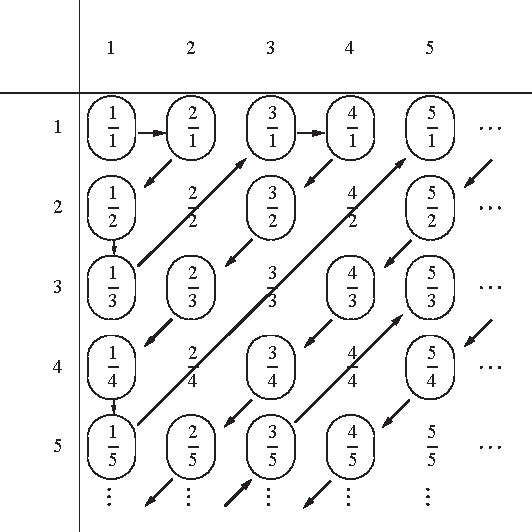
\includegraphics[width=\linewidth]{external/figps-rationals.pdf}
\end{image}%
\tcblower
\end{figureptx}%
The top row in \hyperref[x:figure:fig_positiverationals]{Figure~{\xreffont\ref{x:figure:fig_positiverationals}}, p.\,\pageref{x:figure:fig_positiverationals}} represents the numerator of the rational number, and the left column represents the denominator. We follow the arrows in \hyperref[x:figure:fig_positiverationals]{Figure~{\xreffont\ref{x:figure:fig_positiverationals}}, p.\,\pageref{x:figure:fig_positiverationals}} to define \(f\x \mathbb{N} \to \mathbb{Q}^+\). The idea is to start in the upper left corner of the table and move to successive diagonals as follows:%
\begin{itemize}[label=\textbullet]
\item{}We start with all fractions in which the sum of the numerator and denominator is 2 \(\left( \text{ only } \dfrac{1}{1} \right)\). So \(f ( 1 ) = \dfrac{1}{1}\).%
\item{}We next use those fractions in which the sum of the numerator and denominator is 3. So \(f ( 2 ) = \dfrac{2}{1}\) and \(f ( 3 ) = \dfrac{1}{2}\).%
\item{}We next use those fractions in which the sum of the numerator and denominator is 4. So \(f ( 4 ) = \dfrac{1}{3}\), \(f ( 5 ) = \dfrac{3}{1}\). We skipped \(\dfrac{2}{2}\) since \(\dfrac{2}{2} = \dfrac{1}{1}\). In this way, we will ensure that the function \(f\) is a one-to-one function.%
\end{itemize}
%
\par
We now continue with successive diagonals omitting fractions that are not in lowest terms. This process guarantees that the function \(f\) will be an injection and a surjection. Therefore, \(\mathbb{N} \approx \mathbb{Q}^+\) and \(\text{ card} ( \mathbb{Q}^+ ) = \aleph_0\).%
\end{proof}
Note: For another proof of \hyperref[x:theorem:T_positiverationals]{Theorem~{\xreffont\ref{x:theorem:T_positiverationals}}, p.\,\pageref{x:theorem:T_positiverationals}}, see \hyperref[x:activity:A_Qcountable]{Activity~{\xreffont\ref{x:activity:A_Qcountable}}, p.\,\pageref{x:activity:A_Qcountable}}.%
\par
Since \(\mathbb{Q}^+\) is countable, it seems reasonable to expect that \(Q\) is countable. We will explore this soon. On the other hand, at this point, it may also seem reasonable to ask, ``Are there any uncountable sets?'' The answer to this question is yes, but we will wait until the next section to prove that certain sets are uncountable. We still have a few more issues to deal with concerning countable sets.%
\end{subsectionptx}
%
%
\typeout{************************************************}
\typeout{Subsection  Countably Infinite Sets}
\typeout{************************************************}
%
\begin{subsectionptx}{Countably Infinite Sets}{}{Countably Infinite Sets}{}{}{g:subsection:idm815620120}
\begin{theorem}{}{}{x:theorem:T_addonetocountable}%
If \(A\) is a countably infinite set, then \(A \cup \left\{ x \right\}\) is a countably infinite set.%
\end{theorem}
\begin{proof}{}{g:proof:idm815618328}
Let \(A\) be a countably infinite set. Then there exists a bijection \(f\x \mathbb{N} \to A\). Since \(x\) is either in \(A\) or not in \(A\), we can consider two cases.%
\par
If \(x \in A\), then \(A \cup \left\{ x \right\} = A\) and \(A \cup \left\{ x \right\}\) is countably infinite.%
\par
If \(x \notin A\), define \(g\x \mathbb{N} \to A \cup \left\{ x \right\}\) by%
\begin{equation*}
g( n ) = \begin{cases}x \amp \text{ if \(n = 1\) }  \\ f ( n - 1 )   
\amp \text{ if \(n > 1\). } \end{cases}
\end{equation*}
%
\par
The proof that the function \(g\) is a bijection is \hyperlink{x:exercise:exer_addonetocountable}{Exercise~{\xreffont 4}, p.\,\pageref{x:exercise:exer_addonetocountable}}. Since \(g\) is a bijection, we have proved that \(A \cup \left\{ x \right\} \approx \N\) and hence, \(A \cup \left\{ x \right\}\) is countably infinite.%
\end{proof}
\begin{theorem}{}{}{x:theorem:T_addfinitetocountable}%
If \(A\) is a countably infinite set and \(B\) is a finite set, then \(A \cup B\) is a countably infinite set.%
\end{theorem}
\begin{proof}{}{g:proof:idm815612184}
\hyperlink{x:exercise:exer_addfinitetocountable}{Exercise~{\xreffont 5}, p.\,\pageref{x:exercise:exer_addfinitetocountable}}.%
\end{proof}
\hyperref[x:theorem:T_addfinitetocountable]{Theorem~{\xreffont\ref{x:theorem:T_addfinitetocountable}}, p.\,\pageref{x:theorem:T_addfinitetocountable}} says that if we add a finite number of elements to a countably infinite set, the resulting set is still countably infinite. In other words, the cardinality of the new set is the same as the cardinality of the original set. Finite sets behave very differently in the sense that if we add elements to a finite set, we will change the cardinality. What may even be more surprising is the result in \hyperref[x:theorem:T_unionofcountable]{Theorem~{\xreffont\ref{x:theorem:T_unionofcountable}}, p.\,\pageref{x:theorem:T_unionofcountable}} that states that the union of two countably infinite (disjoint) sets is countably infinite. The proof of this result is similar to the proof that the integers are countably infinite (\hyperref[x:theorem:T_ZequivtoN]{Theorem~{\xreffont\ref{x:theorem:T_ZequivtoN}}, p.\,\pageref{x:theorem:T_ZequivtoN}}). In fact, if \(A = \{a_1, a_2, a_3, \ldots \}\) and \(B = \{b_1, b_2, b_3, \ldots \}\), then we can use the following diagram to help define a bijection from \(\N\) to \(A \cup B\).%
\begin{figureptx}{A Function from \(\N\) to \(A \cup B\)}{x:figure:fig_functionNtoAorB}{}%
\begin{center}%
{\tabularfont%
\begin{tabular}{ccccccccccc}
1&2&3&4&5&6&7&8&9&10&\(\cdots\)\tabularnewline[0pt]
\(\downarrow\)&\(\downarrow\)&\(\downarrow\)&\(\downarrow\)&\(\downarrow\)&\(\downarrow\)&\(\downarrow\)&\(\downarrow\)&\(\downarrow\)&\(\downarrow\)&\(\cdots\)\tabularnewline[0pt]
\(a_1\)&\(b_1\)&\(a_2\)&\(b_2\)&\(a_3\)&\(b_3\)&\(a_4\)&\(b_4\)&\(a_5\)&\(b_5\)&\(\cdots\)
\end{tabular}
}%
\end{center}%
\tcblower
\end{figureptx}%
\begin{theorem}{}{}{x:theorem:T_unionofcountable}%
\index{countably infinite sets!union of}%
If \(A\) and \(B\) are disjoint countably infinite sets, then \(A \cup B\) is a countably infinite set.%
\end{theorem}
\begin{proof}{}{g:proof:idm815585304}
Let \(A\) and \(B\) be countably infinite sets and let \(f\x \mathbb{N} \to A\) and \(g\x \mathbb{N} \to B\) be bijections. Define \(h\x \mathbb{N} \to A \cup B\) by%
\begin{equation*}
h( n ) = \begin{cases}f \!\left( \dfrac{n+1}{2} \right) \amp \text{ if \(n\) is odd }  \\ 
\amp  \\ g \!\left( \dfrac{n}{2} \right) \amp \text{ if \(n\) is even } . \end{cases}
\end{equation*}
%
\par
It is left as \hyperlink{x:exercise:exer_unionofcountable}{Exercise~{\xreffont 6}, p.\,\pageref{x:exercise:exer_unionofcountable}} to prove that the function \(h\) is a bijection.%
\end{proof}
Since we can write the set of rational numbers \(\Q\) as the union of the set of nonnegative rational numbers and the set of negative rational numbers, we can use the results in \hyperref[x:theorem:T_positiverationals]{Theorem~{\xreffont\ref{x:theorem:T_positiverationals}}, p.\,\pageref{x:theorem:T_positiverationals}}, \hyperref[x:theorem:T_addonetocountable]{Theorem~{\xreffont\ref{x:theorem:T_addonetocountable}}, p.\,\pageref{x:theorem:T_addonetocountable}}, and \hyperref[x:theorem:T_unionofcountable]{Theorem~{\xreffont\ref{x:theorem:T_unionofcountable}}, p.\,\pageref{x:theorem:T_unionofcountable}} to prove the following theorem.%
\begin{theorem}{}{}{x:theorem:T_Qiscountable}%
The set \(\mathbb{Q}\) of all rational numbers is countably infinite.%
\end{theorem}
\begin{proof}{}{g:proof:idm815581848}
\hyperlink{x:exercise:exer_Qiscountable}{Exercise~{\xreffont 7}, p.\,\pageref{x:exercise:exer_Qiscountable}}.%
\end{proof}
\index{countably infinite sets!subsets of} In \hyperref[x:section:S_finitesets]{Section~{\xreffont\ref{x:section:S_finitesets}}, p.\,\pageref{x:section:S_finitesets}}, we proved that any subset of a finite set is finite (\hyperref[x:theorem:T_finitesubsets]{Theorem~{\xreffont\ref{x:theorem:T_finitesubsets}}, p.\,\pageref{x:theorem:T_finitesubsets}}). A similar result should be expected for countable sets. We first prove that every subset of \(\mathbb{N}\) is countable. For an infinite subset \(B\) of \(\mathbb{N}\), the idea of the proof is to define a function \(g\x \mathbb{N} \to B\) by removing the elements from \(B\) from smallest to the next smallest to the next smallest, and so on. We do this by defining the function \(g\) recursively as follows:%
\begin{itemize}[label=\textbullet]
\item{}Let \(g ( 1 )\) be the smallest natural number in \(B\).%
\item{}Remove \(g ( 1 )\) from \(B\) and let \(g ( 2 )\) be the smallest natural number in \(B - \left\{ g ( 1 ) \right\}\).%
\item{}Remove \(g ( 2 )\) and let \(g ( 3 )\) be the smallest natural number in \(B - \left\{ g ( 1 ), g ( 2 ) \right\}\).%
\item{}We continue this process. The formal recursive definition of \(g\x \mathbb{N} \to B\) is included in the proof of \hyperref[x:theorem:T_subsetsofN]{Theorem~{\xreffont\ref{x:theorem:T_subsetsofN}}, p.\,\pageref{x:theorem:T_subsetsofN}}.%
\end{itemize}
%
\begin{theorem}{}{}{x:theorem:T_subsetsofN}%
Every subset of the natural numbers is countable.%
\end{theorem}
\begin{proof}{}{g:proof:idm815564568}
Let \(B\) be a subset of \(\mathbb{N}\). If \(B\) is finite, then \(B\) is countable. So we next assume that \(B\) is infinite. We will next give a recursive definition of a function \(g\x \mathbb{N} \to B\) and then prove that \(g\) is a bijection.%
\begin{itemize}[label=\textbullet]
\item{}Let \(g ( 1 )\) be the smallest natural number in \(B\).%
\item{}For each \(n \in \mathbb{N}\), the set \(B - \left\{ g ( 1 ), g ( 2 ), \ldots,
g ( n ) \right\}\) is not empty since \(B\) is infinite. Define \(g ( n + 1 )\) to be the smallest natural number in \(B - \left\{ g ( 1 ), g ( 2 ), \ldots,
g ( n ) \right\}\).%
\end{itemize}
%
\par
The proof that the function \(g\) is a bijection is \hyperlink{x:exercise:exer_subsetofN}{Exercise~{\xreffont 11}, p.\,\pageref{x:exercise:exer_subsetofN}}.%
\end{proof}
\begin{corollary}{}{}{x:corollary:C_subsetofcountable}%
Every subset of a countable set is countable.%
\end{corollary}
\begin{proof}{}{g:proof:idm815558040}
\hyperlink{x:exercise:exer_subsetofcountable}{Exercise~{\xreffont 12}, p.\,\pageref{x:exercise:exer_subsetofcountable}}.%
\end{proof}
\end{subsectionptx}
%
%
\typeout{************************************************}
\typeout{Exercises  Exercises}
\typeout{************************************************}
%
\begin{exercises-subsection}{Exercises}{}{Exercises}{}{}{g:exercises:idm815558808}
\begin{divisionexercise}{1}{}{}{x:exercise:exer_sec93-1}%
State whether each of the following is true or false.%
\begin{enumerate}[font=\bfseries,label=(\alph*),ref=\alph*]
\item{}If a set \(A\) is countably infinite, then \(A\) is infinite.%
\space\hyperlink{g:answer:idm815556632-back}{[Answer]}\item{}If a set \(A\) is countably infinite, then \(A\) is countable.%
\space\hyperlink{g:answer:idm815550360-back}{[Answer]}\item{}If a set \(A\) is uncountable, then \(A\) is not countably infinite.%
\space\hyperlink{g:answer:idm815551768-back}{[Answer]}\item{}If \(A \approx \mathbb{N}_k\) for some \(k \in \mathbb{N}\), then \(A\) is not countable.%
\space\hyperlink{g:answer:idm815550104-back}{[Answer]}\end{enumerate}
\end{divisionexercise}%
\begin{divisionexercise}{2}{}{}{x:exercise:exer_sec93-2}%
Prove that each of the following sets is countably infinite.%
\begin{enumerate}[font=\bfseries,label=(\alph*),ref=\alph*]
\item{}The set \(F^+\) of all natural numbers that are multiples of 5%
\space\hyperlink{g:answer:idm815553432-back}{[Answer]}\item{}The set \(F\) of all integers that are multiples of 5%
\item{}\(\left\{ \left. \dfrac{1}{2^k} \right| k \in \mathbb{N} \right\}\)%
\item{}\(\left\{ n \in \mathbb{Z} \mid n \geq -10 \right\}\)%
\item{}\(\mathbb{N} - \left\{ 4, 5, 6 \right\}\)%
\space\hyperlink{g:answer:idm815544216-back}{[Answer]}\item{}\(\left\{ m \in \mathbb{Z} \mid m \equiv 2 \pmod 3 \right\}\)%
\space\hyperlink{g:answer:idm815542936-back}{[Answer]}\end{enumerate}
\end{divisionexercise}%
\begin{divisionexercise}{3}{}{}{x:exercise:exer_subsetisinfinite}%
Prove \hyperlink{x:li:T_subsetisinfinite2}{Item~{\xreffont 2}, p.\,\pageref{x:li:T_subsetisinfinite2}} of \hyperref[x:theorem:T_subsetisinfinite]{Theorem~{\xreffont\ref{x:theorem:T_subsetisinfinite}}, p.\,\pageref{x:theorem:T_subsetisinfinite}}.%
\space\hyperlink{g:hint:idm815538584-back}{[Hint]}\space\hyperlink{g:answer:idm815533080-back}{[Answer]}\end{divisionexercise}%
\begin{divisionexercise}{4}{}{}{x:exercise:exer_addonetocountable}%
Complete the proof of \hyperref[x:theorem:T_addonetocountable]{Theorem~{\xreffont\ref{x:theorem:T_addonetocountable}}, p.\,\pageref{x:theorem:T_addonetocountable}} by proving the following: Let \(A\) be a countably infinite set and \(x \notin A\). If \(f\x \mathbb{N} \to A\) is a bijection, then \(g\) is a bijection, where \(g\x \mathbb{N} \to A \cup \left\{ x \right\}\) by%
\begin{equation*}
g( n ) = \begin{cases}x \amp \text{ if \(n = 1\) }  \\ f ( n - 1 )   
\amp \text{ if \(n > 1\) } . \end{cases}
\end{equation*}
%
\end{divisionexercise}%
\begin{divisionexercise}{5}{}{}{x:exercise:exer_addfinitetocountable}%
Prove \hyperref[x:theorem:T_addfinitetocountable]{Theorem~{\xreffont\ref{x:theorem:T_addfinitetocountable}}, p.\,\pageref{x:theorem:T_addfinitetocountable}}.%
\par
If \(A\) is a countably infinite set and \(B\) is a finite set, then \(A \cup B\) is a countably infinite set.%
\space\hyperlink{g:hint:idm815523736-back}{[Hint]}\end{divisionexercise}%
\begin{divisionexercise}{6}{}{}{x:exercise:exer_unionofcountable}%
Complete the proof of \hyperref[x:theorem:T_unionofcountable]{Theorem~{\xreffont\ref{x:theorem:T_unionofcountable}}, p.\,\pageref{x:theorem:T_unionofcountable}} by proving the following: Let \(A\) and \(B\) be disjoint countably infinite sets and let \(f\x \mathbb{N} \to A\) and \(g\x \mathbb{N} \to B\) be bijections. Define \(h\x \mathbb{N} \to A \cup B\) by%
\begin{equation*}
h( n ) = \begin{cases}f \!\left( \dfrac{n+1}{2} \right) 
\amp \text{ if \(n\) is odd }  \\ \amp  \\ g \!\left( \dfrac{n}{2} \right)                          \amp \text{ if \(n\) is even } . \end{cases}
\end{equation*}
Then the function \(h\) is a bijection.%
\space\hyperlink{g:answer:idm815523096-back}{[Answer]}\end{divisionexercise}%
\begin{divisionexercise}{7}{}{}{x:exercise:exer_Qiscountable}%
Prove \hyperref[x:theorem:T_Qiscountable]{Theorem~{\xreffont\ref{x:theorem:T_Qiscountable}}, p.\,\pageref{x:theorem:T_Qiscountable}}.%
\par
The set \(\mathbb{Q}\) of all rational numbers is countable.%
\space\hyperlink{g:hint:idm815357848-back}{[Hint]}\space\hyperlink{g:answer:idm815358360-back}{[Answer]}\end{divisionexercise}%
\begin{divisionexercise}{8}{}{}{x:exercise:exer_countinf-finite}%
Prove that if \(A\) is countably infinite and \(B\) is finite, then \(A - B\) is countably infinite.%
\space\hyperlink{g:answer:idm815352472-back}{[Answer]}\end{divisionexercise}%
\begin{divisionexercise}{9}{}{}{x:exercise:exer_NxNbijection}%
Define \(f\x \mathbb{N} \times \mathbb{N} \to \mathbb{N}\) as follows: For each \(( m, n ) \in \mathbb{N} \times \mathbb{N}\),%
\begin{equation*}
f ( m, n ) = 2^{m-1} (2n - 1 )\text{.}
\end{equation*}
%
\begin{enumerate}[font=\bfseries,label=(\alph*),ref=\alph*]
\item{}Prove that \(f\) is an injection.%
\space\hyperlink{g:hint:idm815348376-back}{[Hint]}\item{}Prove that \(f\) is a surjection.%
\space\hyperlink{g:hint:idm815343768-back}{[Hint]}\item{}Prove that \(\mathbb{N} \times \mathbb{N} \approx \mathbb{N}\) and hence that \(\text{ card} \left( \mathbb{N} \times \mathbb{N} \right) = \aleph_0\).%
\end{enumerate}
\end{divisionexercise}%
\begin{divisionexercise}{10}{}{}{g:exercise:idm815342744}%
Use \hyperlink{x:exercise:exer_NxNbijection}{Exercise~{\xreffont 9}, p.\,\pageref{x:exercise:exer_NxNbijection}} to prove that if \(A\) and \(B\) are countably infinite sets, then \(A \times B\) is a countably infinite set.%
\end{divisionexercise}%
\begin{divisionexercise}{11}{}{}{x:exercise:exer_subsetofN}%
Complete the proof of \hyperref[x:theorem:T_subsetsofN]{Theorem~{\xreffont\ref{x:theorem:T_subsetsofN}}, p.\,\pageref{x:theorem:T_subsetsofN}} by proving that the function \(g\) defined in the proof is a bijection from \(\mathbb{N}\) to \(B\).%
\space\hyperlink{g:hint:idm815338648-back}{[Hint]}\end{divisionexercise}%
\begin{divisionexercise}{12}{}{}{x:exercise:exer_subsetofcountable}%
Prove \hyperref[x:corollary:C_subsetofcountable]{Corollary~{\xreffont\ref{x:corollary:C_subsetofcountable}}, p.\,\pageref{x:corollary:C_subsetofcountable}}, which states that every subset of a countable set is countable.%
\space\hyperlink{g:hint:idm815331992-back}{[Hint]}\end{divisionexercise}%
\begin{divisionexercise}{13}{}{}{g:exercise:idm815326360}%
Use \hyperref[x:corollary:C_subsetofcountable]{Corollary~{\xreffont\ref{x:corollary:C_subsetofcountable}}, p.\,\pageref{x:corollary:C_subsetofcountable}} to prove that the set of all rational numbers between 0 and 1 is countably infinite.%
\end{divisionexercise}%
\begin{divisionexercise}{14}{}{}{x:exercise:exer_tworationals}%
Let \(a, b \in \mathbb{Q}\) with \(a \lt  b\). In \hyperref[x:subsection:tworationals]{The Set of Positive Rational Numbers, p.\,\pageref{x:subsection:tworationals}}, we proved that \(c = \dfrac{a+b}{2}\) is a rational number and that \(a \lt  c \lt  b\), which proves that here is a rational number between any two (unequal) rational numbers.%
\begin{enumerate}[font=\bfseries,label=(\alph*),ref=\alph*]
\item{}Now let \(c_1 = \dfrac{a+b}{2}\), and define \(c_2 = \dfrac{c_1 + b}{2}\). Prove that \(c_1 \lt c_2 \lt b\) and hence, that \(a \lt c_1 \lt c_2 \lt b\).%
\item{}For each \(k \in \mathbb{N}\), define%
\begin{equation*}
c_{k+1} = \frac{c_k + b}{2}\text{.}
\end{equation*}
Prove that for each \(k \in \mathbb{N}\), \(a \lt  c_k \lt  c_{k+1} \lt  b\). Use this to explain why the set \(\left\{ c_k \mid k \in \mathbb{N} \right\}\) is an infinite set where each element is a rational number between \(a\) and \(b\).%
\end{enumerate}
\end{divisionexercise}%
\begin{activity}{Another Proof that \(\mathbf{\Q^+}\) Is Countable.}{x:activity:A_Qcountable}%
For this activity, it may be helpful to use the Fundamental Theorem of Arithmetic (see \hyperref[x:theorem:T_fundtheorem]{Theorem~{\xreffont\ref{x:theorem:T_fundtheorem}}, p.\,\pageref{x:theorem:T_fundtheorem}}. Let \(\Q^+\) be the set of positive rational numbers. Every positive rational number has a unique representation as a fraction \(\dfrac{m}{n}\), where \(m\) and \(n\) are relatively prime natural numbers. We will now define a function \(f\x  \Q^+ \to \N\) as follows:%
\par
If \(x \in \Q^+\) and \(x = \dfrac{m}{n}\), where \(m,
n \in \N\), \(n \ne 1\) and \(\gcd(m, n) = 1\), we write%
\begin{align*}
m \amp = p_1^{\alpha_1} p_2^{\alpha_2} \cdots p_r^{\alpha_r}, \text{ and }\\
n \amp = q_1^{\beta_1} q_2^{\beta_2} \cdots q_s^{\beta_s}\text{,}
\end{align*}
where \(p_1\), \(p_2\), \textellipsis{}, \(p_r\) are distinct prime numbers, \(q_1\), \(q_2\), \textellipsis{}, \(q_s\) are distinct prime numbers, and \(\alpha_1\), \(\alpha_2\), \textellipsis{}, \(\alpha_r\) and \(\beta_1\), \(\beta_2\), \textellipsis{}, \(\beta_s\) are natural numbers. We also write \(1 = 2^0\) when \(m = 1\). We then define%
\begin{equation*}
f(x) = p_1^{2\alpha_1} p_2^{2\alpha_2} \cdots p_r^{2\alpha_r} q_1^{2\beta_1 -1 } 
q_2^{2 \beta_2 - 1} \cdots q_s^{2 \beta_s - 1}\text{.}
\end{equation*}
If \(x = \dfrac{m}{1}\), then we define \(f(x) = p_1^{2\alpha_1} p_2^{2\alpha_2} \cdots p_r^{2\alpha_r} = m^2\).%
\begin{enumerate}[font=\bfseries,label=(\alph*),ref=\alph*]
\item{}Determine \(f \!\left( \dfrac{2}{3} \right)\), \(f \!\left( \dfrac{5}{6} \right)\), \(f ( 6 )\), \(f ( \dfrac{12}{25} )\), \(f \!\left( \dfrac{375}{392} \right)\), and \(f \!\left( \dfrac{2^3 \cdot 11^3}{3 \cdot 5^4} \right)\).%
\item{}If possible, find \(x \in \Q^+\) such that \(f(x) = 100\).%
\item{}If possible, find \(x \in \Q^+\) such that \(f(x) = 12\).%
\item{}If possible, find \(x \in \Q^+\) such that \(f(x) = 2^8 \cdot 3^5 \cdot 13 \cdot 17^2\).%
\item{}Prove that the function \(f\) is an injection.%
\item{}Prove that the function \(f\) is a surjection.%
\item{}What has been proved?%
\end{enumerate}
\end{activity}%
\end{exercises-subsection}
\end{sectionptx}
%
%
\typeout{************************************************}
\typeout{Section 9.3 Uncountable Sets}
\typeout{************************************************}
%
\begin{sectionptx}{Uncountable Sets}{}{Uncountable Sets}{}{}{x:section:S_uncountablesets}
%
%
\typeout{************************************************}
\typeout{Beginning Activity  The Game of Dodge Ball}
\typeout{************************************************}
%
\begin{worksheet-subsection}{The Game of Dodge Ball}{}{The Game of Dodge Ball}{}{}{x:worksheet:PA_dodgeball}
\index{Dodge Ball}%
(From \pubtitle{The Heart of Mathematics: An Invitation to Effective Thinking} by Edward B. Burger and Michael Starbird, Key Publishing Company, \textcopyright{} 2000 by Edward B. Burger and Michael Starbird.)%
\par
Dodge Ball is a game for two players. It is played on a game board such as the one shown in \hyperref[x:figure:fig_dodgeball1]{Figure~{\xreffont\ref{x:figure:fig_dodgeball1}}, p.\,\pageref{x:figure:fig_dodgeball1}} and \hyperref[x:figure:fig_dodgeball2]{Figure~{\xreffont\ref{x:figure:fig_dodgeball2}}, p.\,\pageref{x:figure:fig_dodgeball2}}.%
\begin{figureptx}{Game Board for Dodge Ball: Player 1}{x:figure:fig_dodgeball1}{}%
\begin{image}{0.1}{0.8}{0.1}%
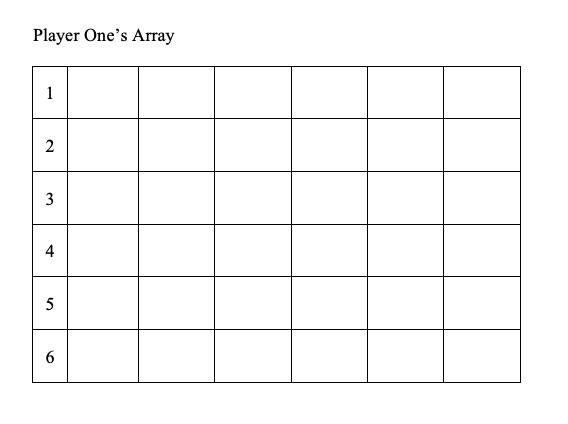
\includegraphics[width=\linewidth]{external/figps-sec93-dodgeball-player1.png}
\end{image}%
\tcblower
\end{figureptx}%
\begin{figureptx}{Game Board for Dodge Ball: Player 2}{x:figure:fig_dodgeball2}{}%
\begin{image}{0.1}{0.8}{0.1}%
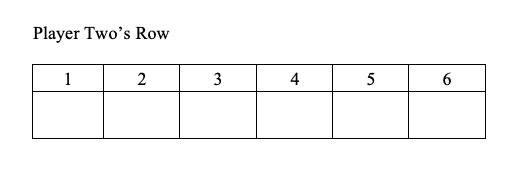
\includegraphics[width=\linewidth]{external/figps-sec93-dodgeball-player2.png}
\end{image}%
\tcblower
\end{figureptx}%
Player One has a 6 by 6 array to complete and Player Two has a 1 by 6 row to complete. Each player has six turns as described next.%
\begin{itemize}[label=\textbullet]
\item{}Player One begins by filling in the first horizontal row of his or her table with a sequence of six X's and O's, one in each square in the first row.%
\item{}Then Player Two places either an X or an O in the first box of his or her row. At this point, Player One has completed the first row and Player Two has filled in the first box of his or her row with one letter.%
\item{}The game continues with Player One completing a row with six letters (X's and O's), one in each box of the next row followed by Player Two writing one letter (an X or an O) in the next box of his or her row. The game is completed when Player One has completed all six rows and Player Two has completed all six boxes in his or her row.%
\end{itemize}
%
\par
%
\begin{itemize}[label=\textbullet]
\item{}Player One wins if any horizontal row in the 6 by 6 array is identical to the row that Player Two created. (Player One matches Player Two.)%
\item{}Player Two wins if Player Two's row of six letters is different than each of the six rows produced by Player One. (Player Two ``dodges'' Player One.)%
\end{itemize}
%
\par
There is a winning strategy for one of the two players. This means that there is plan by which one of the two players will always win. Which player has a winning strategy? Carefully describe this winning strategy.%
\begin{paragraphs}{Applying the Winning Strategy to Lists of Real Numbers.}{g:paragraphs:idm815282584}%
Following is a list of real numbers between 0 and 1. Each real number is written as a decimal number.%
\begin{align*}
a_1 \amp = 0.1234567890   \amp   a_6 \amp = 0.0103492222\\
a_2 \amp = 0.3216400000   \amp   a_7 \amp = 0.0011223344\\
a_3 \amp = 0.4321593333   \amp   a_8 \amp = 0.7077700022\\
a_4 \amp = 0.9120930092   \amp   a_9 \amp = 0.2100000000\\
a_5 \amp = 0.0000234102   \amp  a_{10} \amp = 0.9870008943
\end{align*}
%
\par
Use a method similar to the winning strategy in the game of Dodge Ball to write a real number (in decimal form) between 0 and 1 that is not in this list of 10 numbers.%
\end{paragraphs}%
\begin{divisionexercise}{1}{}{}{g:exercise:idm815283224}%
Do you think your method could be used for any list of 10 real numbers between 0 and 1 if the goal is to write a real number between 0 and 1 that is not in the list?%
\end{divisionexercise}%
\begin{divisionexercise}{2}{}{}{g:exercise:idm815285784}%
Do you think this method could be extended to a list of 20 different real numbers? To a list of 50 different real numbers?%
\end{divisionexercise}%
\begin{divisionexercise}{3}{}{}{g:exercise:idm815277976}%
Do you think this method could be extended to a countably infinite list of real numbers?%
\end{divisionexercise}%
\end{worksheet-subsection}
%
%
\typeout{************************************************}
\typeout{Beginning Activity  Beginning Activity 2: Functions from a Set to Its Power Set}
\typeout{************************************************}
%
\begin{worksheet-subsection}{Beginning Activity 2: Functions from a Set to Its Power Set}{}{Beginning Activity 2: Functions from a Set to Its Power Set}{}{}{x:worksheet:PA_powerset}
\index{power set}%
Let \(A\) be a set. In \hyperref[x:section:S_setoperations]{Section~{\xreffont\ref{x:section:S_setoperations}}, p.\,\pageref{x:section:S_setoperations}}, we defined the \terminology{power set} \(\mathcal{P} ( A )\) of \(A\) to be the set of all subsets of \(A\). This means that \(X \in \mathcal{P} ( A )\) if and only if \(X \subseteq A\). \hyperref[x:theorem:T_powerset]{Theorem~{\xreffont\ref{x:theorem:T_powerset}}, p.\,\pageref{x:theorem:T_powerset}} in \hyperref[x:section:S_setoperations]{Section~{\xreffont\ref{x:section:S_setoperations}}, p.\,\pageref{x:section:S_setoperations}} states that if a set \(A\) has \(n\) elements, then \(A\) has \(2^n\) subsets or that \(\mathcal{P} ( A )\) has \(2^n\) elements. Using our current notation for cardinality, this means that if \(\text{ card} ( A ) = n\), then \(\text{ card} ( \mathcal{P} ( A ) ) = 2^n\). (The proof of this theorem was \hyperref[x:activity:exer_powerset]{Activity~{\xreffont\ref{x:activity:exer_powerset}}, p.\,\pageref{x:activity:exer_powerset}}.)%
\par
We are now going to define and explore some functions from a set \(A\) to its power set \(\mathcal{P} ( A )\). This means that the input of the function will be an element of \(A\) and the output of the function will be a subset of \(A\).%
\begin{divisionexercise}{1}{}{}{g:exercise:idm815264920}%
Let \(A = \left\{1, 2, 3, 4 \right\}\). Define \(f\x A \to \mathcal{P} ( A )\) by%
\begin{align*}
f ( 1 ) \amp = \left\{ 1, 2, 3 \right\} \amp f ( 2 ) \amp = \left\{ 1, 3, 4 \right\}\\
f ( 3 ) \amp = \left\{ 1, 4 \right\} \amp f ( 4 ) \amp = \left\{ 2, 4 \right\}
\end{align*}
%
\begin{enumerate}[font=\bfseries,label=(\alph*),ref=\alph*]
\item{}Is \(1 \in f ( 1 )\)? Is \(2 \in f ( 2 )\)? Is \(3 \in f ( 3 )\)? Is \(4 \in f ( 4 )\)?%
\item{}Determine \(S = \left\{ x \in A \mid x \notin f ( x ) \right\}\).%
\item{}Notice that \(S \in \mathcal{P} ( A )\). Does there exist an element \(t\) in \(A\) such that \(f ( t ) = S\)? That is, is \(S \in \text{ range} ( f )\)?%
\end{enumerate}
\end{divisionexercise}%
\begin{divisionexercise}{2}{}{}{g:exercise:idm815266328}%
Let \(A = \left\{1, 2, 3, 4 \right\}\). Define \(f\x A \to \mathcal{P} ( A )\) by%
\begin{equation*}
f ( x ) = A - \left\{ x \right\} \text{ for each } x \in A\text{.}
\end{equation*}
%
\begin{enumerate}[font=\bfseries,label=(\alph*),ref=\alph*]
\item{}Determine \(f ( 1 )\). Is \(1 \in f ( 1 )\)?%
\item{}Determine \(f ( 2 )\). Is \(2 \in f ( 2 )\)?%
\item{}Determine \(f ( 3 )\). Is \(3 \in f ( 3 )\)?%
\item{}Determine \(f ( 4 )\). Is \(4 \in f ( 4 )\)?%
\item{}Determine \(S = \left\{ x \in A \mid x \notin f ( x ) \right\}\).%
\item{}Notice that \(S \in \mathcal{P} ( A )\). Does there exist an element \(t\) in \(A\) such that \(f ( t ) = S\)? That is, is \(S \in \text{ range} ( f )\)?%
\end{enumerate}
\end{divisionexercise}%
\begin{divisionexercise}{3}{}{}{g:exercise:idm815245080}%
Define \(f\x \mathbb{N} \to \mathcal{P} ( \mathbb{N} )\) by%
\begin{equation*}
f ( n ) = \mathbb{N} - \left\{n^2, n^2-2n \right\},
\text{ for each } n \in \mathbb{N}\text{.}
\end{equation*}
%
\begin{enumerate}[font=\bfseries,label=(\alph*),ref=\alph*]
\item{}Determine \(f ( 1 )\), \(f ( 2 )\), \(f ( 3 )\), and \(f ( 4 )\). In each of these cases, determine if \(k \in f ( k )\).%
\item{}Prove that if \(n > 3\), then \(n \in f ( n )\).%
\par\smallskip%
\noindent\textbf{\blocktitlefont Hint}.\label{g:hint:idm815245592}{}\hypertarget{g:hint:idm815245592}{}\quad{}Prove that if \(n >3\), then \(n^2 > n\) and \(n^2 - 2n >n\).%
\item{}Determine \(S = \left\{ x \in \mathbb{N} \mid x \notin f ( x ) \right\}\).%
\item{}Notice that \(S \in \mathcal{P} ( \mathbb{N} )\). Does there exist an element \(t\) in \(\mathbb{N}\) such that \(f ( t ) = S\)? That is, is \(S \in \text{ range} ( f )\)?%
\end{enumerate}
\end{divisionexercise}%
\end{worksheet-subsection}
\begin{introduction}{}%
We have seen examples of sets that are countably infinite, but we have not yet seen an example of an infinite set that is uncountable. We will do so in this section. The first example of an uncountable set will be the open interval of real numbers \(( 0, 1 )\). The proof that this interval is uncountable uses a method similar to the winning strategy for Player Two in the game of Dodge Ball from \hyperref[x:worksheet:PA_dodgeball]{Beginning Activity 1, p.\,\pageref{x:worksheet:PA_dodgeball}}. Before considering the proof, we need to state an important result about decimal expressions for real numbers.%
\end{introduction}%
%
%
\typeout{************************************************}
\typeout{Subsection  Decimal Expressions for Real Numbers}
\typeout{************************************************}
%
\begin{subsectionptx}{Decimal Expressions for Real Numbers}{}{Decimal Expressions for Real Numbers}{}{}{g:subsection:idm815237912}
\index{decimal expression!for a real number}%
In its decimal form, any real number \(a\) in the interval \(( 0, 1 )\) can be written as \(a = 0.a_1 a_2 a_3 a_4 \ldots \), where each \(a_i\) is an integer with \(0 \leq a_i \leq 9\). For example,%
\begin{equation*}
\frac{5}{12} = 0.416666 \ldots\text{.}
\end{equation*}
%
\par
We often abbreviate this as \(\dfrac{5}{12} = 0.41 \overline{6}\) to indicate that the \(6\) is repeated. We can also repeat a block of digits. For example, \(\dfrac{5}{26} = 0.19 \overline{230769}\) to indicate that the block 230769 repeats. That is,%
\begin{equation*}
\frac{5}{26} = 0.19230769230769230769 \ldots\text{.}
\end{equation*}
%
\par
There is only one situation in which a real number can be represented as a decimal in more than one way. A decimal that ends with an infinite string of 9's is equal to one that ends with an infinite string of 0's. For example, \(0.3199999 \ldots\) represents the same real number as \(0.3200000 \ldots \). Geometric series can be used to prove that a decimal that ends with an infinite string of 9's is equal to one that ends with an infinite string of 0's, but we will not do so here.%
\begin{assemblage}{Definition.}{x:assemblage:normalized}%
A decimal representation of a real number \(a\) is in \terminology{normalized form} provided that there is no natural number \(k\) such that for all natural numbers \(n\) with \(n > k\), \(a_n = 9\). That is, the decimal representation of \(a\) is in normalized form if and only if it does not end with an infinite string of 9's.%
\end{assemblage}
One reason the normalized form is important is the following theorem (which will not be proved here).%
\begin{theorem}{}{}{x:theorem:T_normalized}%
Two decimal numbers in normalized form are equal if and only if they have identical digits in each decimal position.%
\end{theorem}
\end{subsectionptx}
%
%
\typeout{************************************************}
\typeout{Subsection  Uncountable Subsets of \(\boldsymbol{\mathbb{R}}\)}
\typeout{************************************************}
%
\begin{subsectionptx}{Uncountable Subsets of \(\boldsymbol{\mathbb{R}}\)}{}{Uncountable Subsets of \(\boldsymbol{\mathbb{R}}\)}{}{}{x:subsection:sym_continuum}
In the proof that follows, we will use only the normalized form for the decimal representation of a real number in the interval \(( 0, 1 )\).%
\begin{theorem}{}{}{x:theorem:T_uncountableinterval}%
The open interval \(( 0, 1 )\) is an uncountable set.%
\end{theorem}
\begin{proof}{}{g:proof:idm815224856}
Since the interval \(( 0, 1 )\) contains the infinite subset \(\left\{\dfrac{1}{2}, \dfrac{1}{3}, \dfrac{1}{4}, \ldots \,\right\}\), we can use \hyperref[x:theorem:T_subsetisinfinite]{Theorem~{\xreffont\ref{x:theorem:T_subsetisinfinite}}, p.\,\pageref{x:theorem:T_subsetisinfinite}}, to conclude that \(( 0, 1 )\) is an infinite set. So \(( 0, 1 )\) is either countably infinite or uncountable. We will prove that \(( 0, 1 )\) is uncountable by proving that any function from \(\N\) to \((0, 1)\) is not a surjection, and hence, there is no bijection from \(\N\) to \((0, 1)\).%
\par
So suppose that \(f\x \mathbb{N} \to ( 0, 1 )\) is a function. We will show that \(f\) is not a surjection by showing that there exists an element in \(( 0, 1 )\) that cannot be in the range of \(f\). Writing the images of the elements of \(\mathbb{N}\) in normalized form, we can write%
\begin{align*}
f ( 1 ) \amp = 0.a_{1 1} a_{1 2} a_{1 3} a_{1 4} a_{1 5} \ldots\\
f ( 2 ) \amp = 0.a_{2 1} a_{2 2} a_{2 3} a_{2 4} a_{2 5} \ldots\\
f ( 3 ) \amp = 0.a_{3 1} a_{3 2} a_{3 3} a_{3 4} a_{3 5} \ldots\\
f ( 4 ) \amp = 0.a_{4 1} a_{4 2} a_{4 3} a_{4 4} a_{4 5} \ldots\\
f ( 5 ) \amp = 0.a_{5 1} a_{5 2} a_{5 3} a_{5 4} a_{5 5} \ldots\\
\amp \vdots\\
f ( n ) \amp = 0.a_{n 1} a_{n 2} a_{n 3} a_{n 4} a_{n 5} \ldots\\
\amp \vdots
\end{align*}
%
\par
Notice the use of the double subscripts. The number \(a_{i j}\) is the \(j^\text{ th }\) digit to the right of the decimal point in the normalized decimal representation of \(f ( i )\).%
\par
We will now construct a real number \(b = 0.b_1 b_2 b_3 b_4 b_5 \ldots\) in \(( 0, 1 )\) and in normalized form that is not in this list.%
\par
Note: The idea is to start in the upper left corner and move down the diagonal in a manner similar to the winning strategy for Player Two in the game in \hyperref[x:worksheet:PA_dodgeball]{Beginning Activity 1, p.\,\pageref{x:worksheet:PA_dodgeball}}. At each step, we choose a digit that is not equal to the diagonal digit.%
\par
Start with \(a_{1 1}\) in \(f ( 1 )\). We want to choose \(b_1\) so that \(b_1 \ne 0\), \(b_1 \ne a_{1 1}\), and \(b_1 \ne 9\). (To ensure that we end up with a decimal that is in normalized form, we make sure that each digit is not equal to 9.) We then repeat this process with \(a_{2 2}\), \(a_{3 3}\), \(a_{4 4}\), \(a_{5 5}\), and so on. So we let \(b\) be the real number \(b = 0.b_1 b_2 b_3 b_4 b_5 \ldots \), where for each \(k \in \mathbb{N}\)%
\begin{equation*}
b_k = \begin{cases}3 \amp \text{if \(a_{k k} \ne 3\)}  \\ 5 \amp 
\text{if \(a_{k k} = 3\).} \end{cases}
\end{equation*}
(The choice of 3 and 5 is arbitrary. Other choices of distinct digits will also work.)%
\par
Now for each \(n \in \mathbb{N}\), \(b \ne f ( n )\) since \(b\) and \(f ( n )\) are in normalized form and \(b\) and \(f ( n )\) differ in the \(n\)\textbraceleft{}th\textbraceright{} decimal place. Therefore, \(f\) is not a surjection. This proves that any function from \(\mathbb{N}\) to \(( 0, 1 )\) is not a surjection and hence, there is no bijection from \(\mathbb{N}\) to \(( 0, 1 )\). Therefore, \(( 0, 1 )\) is not countably infinite and hence must be an uncountable set.%
\end{proof}
\begin{inlineexercise}{Dodge Ball and Cantor's Diagonal Argument.}{x:exercise:prog_diagonal}%
\index{Cantor's diagonal argument}%
\index{Dodge Ball}%
The proof of \hyperref[x:theorem:T_uncountableinterval]{Theorem~{\xreffont\ref{x:theorem:T_uncountableinterval}}, p.\,\pageref{x:theorem:T_uncountableinterval}} is often referred to as \terminology{Cantor's diagonal argument}. It is named after the mathematician Georg Cantor, who first published the proof in 1874. Explain the connection between the winning strategy for Player Two in Dodge Ball (see \hyperref[x:worksheet:PA_dodgeball]{Beginning Activity 1, p.\,\pageref{x:worksheet:PA_dodgeball}}) and the proof of \hyperref[x:theorem:T_uncountableinterval]{Theorem~{\xreffont\ref{x:theorem:T_uncountableinterval}}, p.\,\pageref{x:theorem:T_uncountableinterval}} using Cantor's diagonal argument.%
\space\hyperlink{g:solution:idm815201560-back}{[Solution]}\end{inlineexercise}%
\index{continuum} The open interval \(( 0, 1 )\) is our first example of an uncountable set. The cardinal number of \(( 0, 1 )\) is defined to be \(\boldsymbol{c}\), which stands for \terminology{the cardinal number of the continuum}. So the two infinite cardinal numbers we have seen are \(\aleph_0\) for countably infinite sets and \(\boldsymbol{c}\).%
\begin{assemblage}{Definition.}{x:assemblage:cardinalityc}%
\label{g:notation:idm815189016} A set \(A\) is said to have \terminology{cardinality \(\boldsymbol{c}\)} provided that \(A\) is equivalent to \(( 0, 1 )\). In this case, we write \(\text{ card} ( A ) = \boldsymbol{c}\) and say that the cardinal number of \(A\) is \(\boldsymbol{c}\).%
\end{assemblage}
The proof of \hyperref[x:theorem:T_openintervals]{Theorem~{\xreffont\ref{x:theorem:T_openintervals}}, p.\,\pageref{x:theorem:T_openintervals}} is included in \hyperref[x:exercise:prog_openintervals]{Progress Check~{\xreffont\ref{x:exercise:prog_openintervals}}, p.\,\pageref{x:exercise:prog_openintervals}}.%
\begin{theorem}{}{}{x:theorem:T_openintervals}%
Let \(a\) and \(b\) be real numbers with \(a \lt b\). The open interval \(( a, b )\) is uncountable and has cardinality \(\boldsymbol{c}\).%
\end{theorem}
\begin{inlineexercise}{Proof of Theorem~{\xreffont\ref*{x:theorem:T_openintervals}}.}{x:exercise:prog_openintervals}%
\begin{enumerate}[font=\bfseries,label=(\alph*),ref=\alph*]
\item{}In \hyperref[x:task:A_equivsets4]{Task~{\xreffont\ref{x:exercise:prog_equivsets}}.{\xreffont\ref{x:task:A_equivsets4}}, p.\,\pageref{x:task:A_equivsets4}} of \hyperref[x:exercise:prog_equivsets]{Progress Check~{\xreffont\ref{x:exercise:prog_equivsets}}, p.\,\pageref{x:exercise:prog_equivsets}}, we proved that if \(b \in \R\) and \(b > 0\), then the open interval \(( 0, 1 )\) is equivalent to the open interval \(( 0, b )\). Now let \(a\) and \(b\) be real numbers with \(a \lt  b\). Find a function%
\begin{equation*}
f\x  ( 0, 1 ) \to ( a, b )
\end{equation*}
that is a bijection and conclude that the open interval \(( 0, 1) \approx ( a, b )\).%
\space\hyperlink{g:solution:idm815172504-back}{[Solution]}\item{}Let \(a, b, c, d\) be real numbers with \(a \lt b\) and \(c \lt d\). Prove that the open interaval \(( a, b )\) is equivalent to the open interval \(( c, d )\).%
\space\hyperlink{g:solution:idm815155480-back}{[Solution]}\end{enumerate}
\end{inlineexercise}%
\begin{theorem}{}{}{x:theorem:T_realsuncount}%
The set of real numbers \(\mathbb{R}\) is uncountable and has cardinality \(\boldsymbol{c}\).%
\end{theorem}
\begin{proof}{}{g:proof:idm815155096}
Let \(f\x \left( -\dfrac{\pi}{2}, \dfrac{\pi}{2} \right) \to \mathbb{R}\) be defined by \(f ( x ) = \tan x\), for each \(x \in \mathbb{R}\). The function \(f\) is a bijection and, hence, \(\left(-\dfrac{\pi}{2}, \dfrac{\pi}{2} \right) \approx \mathbb{R}\). So by \hyperref[x:theorem:T_openintervals]{Theorem~{\xreffont\ref{x:theorem:T_openintervals}}, p.\,\pageref{x:theorem:T_openintervals}}, \(\mathbb{R}\) is uncountable and has cardinality \(\boldsymbol{c}\).%
\end{proof}
\end{subsectionptx}
%
%
\typeout{************************************************}
\typeout{Subsection  Cantor's Theorem}
\typeout{************************************************}
%
\begin{subsectionptx}{Cantor's Theorem}{}{Cantor's Theorem}{}{}{g:subsection:idm815146776}
\index{Cantor's Theorem}%
\index{Cantor, Georg}%
We have now seen two different infinite cardinal numbers, \(\aleph_0\) and \(\boldsymbol{c}\). It can seem surprising that there is more than one infinite cardinal number. A reasonable question at this point is, ``Are there any other infinite cardinal numbers?'' The astonishing answer is that there are, and in fact, there are infinitely many different infinite cardinal numbers. The basis for this fact is the following theorem, which states that a set is not equivalent to its power set. The proof is due to Georg Cantor (1845\textendash{}1918), and the idea for this proof was explored in \hyperref[x:worksheet:PA_powerset]{Beginning Activity 2, p.\,\pageref{x:worksheet:PA_powerset}}. The basic idea of the proof is to prove that any function from a set \(A\) to its power set cannot be a surjection.%
\begin{theorem}{Cantor's Theorem.}{}{x:theorem:T_cantor}%
For every set \(A\), \(A\) and \(\mathcal{P} ( A )\) do not have the same cardinality.%
\end{theorem}
\begin{proof}{}{g:proof:idm815147544}
Let \(A\) be a set. If \(A = \emptyset\), then \(\mathcal{P} ( A ) = \left\{ \emptyset \right\}\), which has cardinality 1. Therefore, \(\emptyset\) and \(\mathcal{P} ( \emptyset )\) do not have the same cardinality.%
\par
Now suppose that \(A \ne \emptyset\), and let \(f\x  A \to \mathcal{P} ( A )\). We will show that \(f\) cannot be a surjection, and hence there is no bijection from \(A\) to \(\mathcal{P} ( A )\). This will prove that \(A\) is not equivalent to \(\mathcal{P} ( A )\). Define%
\begin{equation*}
S = \left\{ x \in A \mid x \notin f ( x ) \right\}\text{.}
\end{equation*}
%
\par
Assume that there exists a \(t\) in \(A\) such that \(f ( t ) = S\). Now, either \(t \in S\) or \(t \notin S\).%
\begin{itemize}[label=\textbullet]
\item{}If \(t \in S\), then \(t \in \left\{ x \in A \mid x \notin f ( x ) \right\}\). By the definition of \(S\), this means that \(t \notin f ( t )\). However, \(f ( t ) = S\) and so we conclude that \(t \notin S\). But now we have \(t \in S\) and \(t \notin S\). This is a contradiction.%
\item{}If \(t \notin S\), then \(t \notin \left\{ x \in A \mid x \notin f ( x ) \right\}\). By the definition of \(S\), this means that \(t \in f ( t )\). However, \(f ( t ) = S\) and so we conclude that \(t \in S\). But now we have \(t \notin S\) and \(t \in S\). This is a contradiction.%
\end{itemize}
%
\par
So in both cases we have arrived at a contradiction. This means that there does not exist a \(t\) in \(A\) such that \(f ( t ) = S\). Therefore, any function from \(A\) to \(\mathcal{P} ( A )\) is not a surjection and hence not a bijection. Hence, \(A\) and \(\mathcal{P} ( A )\) do not have the same cardinality.%
\end{proof}
\begin{corollary}{}{}{x:corollary:C_cantor}%
\(\mathcal{P} ( \mathbb{N} )\) is an infinite set that is not countably infinite.%
\end{corollary}
\begin{proof}{}{g:proof:idm815127576}
Since \(\mathcal{P} ( \mathbb{N} )\) contains the infinite subset \(\left\{ \left\{ 1 \right\}, \left\{ 2 \right\}, \left\{ 3 \right\} \ldots \,\right\}\), we can use \hyperref[x:theorem:T_subsetisinfinite]{Theorem~{\xreffont\ref{x:theorem:T_subsetisinfinite}}, p.\,\pageref{x:theorem:T_subsetisinfinite}}, to conclude that \(\mathcal{P} ( \mathbb{N} )\) is an infinite set. By Cantor's Theorem (\hyperref[x:theorem:T_cantor]{Theorem~{\xreffont\ref{x:theorem:T_cantor}}, p.\,\pageref{x:theorem:T_cantor}}), \(\mathbb{N}\) and \(\mathcal{P} ( \mathbb{N} )\) do not have the same cardinality. Therefore, \(\mathcal{P} ( \mathbb{N} )\) is not countable and hence is an uncountable set.%
\end{proof}
\end{subsectionptx}
%
%
\typeout{************************************************}
\typeout{Subsection  Some Final Comments about Uncountable Sets}
\typeout{************************************************}
%
\begin{subsectionptx}{Some Final Comments about Uncountable Sets}{}{Some Final Comments about Uncountable Sets}{}{}{g:subsection:idm815129496}
%
\begin{enumerate}
\item\label{x:li:sec94_comment1}{}\hypertarget{x:li:sec94_comment1}{}We have now seen that any open interval of real numbers is uncountable and has cardinality \(\boldsymbol{c}\). In addition, \(\mathbb{R}\) is uncountable and has cardinality \(\boldsymbol{c}\). Now, \hyperref[x:corollary:C_cantor]{Corollary~{\xreffont\ref{x:corollary:C_cantor}}, p.\,\pageref{x:corollary:C_cantor}} tells us that \(\mathcal{P} ( \mathbb{N} )\) is uncountable. A question that can be asked is, ``Does \(\mathcal{P} ( \mathbb{N} )\) have the same cardinality as \(\mathbb{R}\)?'' The answer is yes, although we are not in a position to prove it yet. A proof of this fact uses the following theorem, which is known as the Cantor-Schröder-Bernstein Theorem.%
\begin{theorem}{Cantor-Schröder-Bernstein.}{}{x:theorem:T_bernstein}%
\index{Cantor-Schröder-Bernstein Theorem}Let \(A\) and \(B\) be sets. If there exist injections \(f\x A \to B\) and \(g\x B \to A\), then \(A \approx B\).%
\end{theorem}
In the statement of this theorem, notice that it is not required that the function \(g\) be the inverse of the function \(f\). We will not prove the Cantor-Schröder-Bernstein Theorem here. The following items will show some uses of this important theorem.%
\item{}The Cantor-Schröder-Bernstein Theorem can also be used to prove that the closed interval \([ 0, 1 ]\) is equivalent to the open interval \(( 0, 1 )\). See \hyperlink{x:exercise:exer_closedinterval}{Exercise~{\xreffont 6}, p.\,\pageref{x:exercise:exer_closedinterval}}.%
\item\label{x:li:sec94_comment3}{}\hypertarget{x:li:sec94_comment3}{}Another question that was posed earlier is, ``Are there other infinite cardinal numbers other than \(\aleph_0\) and \(\boldsymbol{c}\)?'' Again, the answer is yes, and the basis for this is Cantor's Theorem (\hyperref[x:theorem:T_cantor]{Theorem~{\xreffont\ref{x:theorem:T_cantor}}, p.\,\pageref{x:theorem:T_cantor}}). We can start with \(\text{ card} ( \mathbb{N} ) = \aleph_0\). We then define the following infinite cardinal numbers:%
\begin{align*}
\amp \text{ card} ( \mathcal{P} ( \mathbb{N} ) ) = \alpha_1 \amp \amp
\text{ card} ( \mathcal{P} ( \mathcal{P} ( \mathbb{N} ) ) ) = \alpha_2\\
\amp \text{ card} ( \mathcal{P} ( \mathcal{P} ( \mathcal{P} 
( \mathbb{N} ) ) ) ) = \alpha_3 \amp \amp \vdots
\end{align*}
%
\par
Cantor's Theorem tells us that these are all different cardinal numbers, and so we are just using the lowercase Greek letter \(\alpha\) (alpha) to help give names to these cardinal numbers. In fact, although we will not define it here, there is a way to ``order'' these cardinal numbers in such a way that%
\begin{equation*}
\aleph_0 \lt  \alpha_1 \lt  \alpha_2 \lt  \alpha_3 \lt  \cdots\text{.}
\end{equation*}
Keep in mind, however, that even though these are different cardinal numbers, Cantor's Theorem does not tell us that these are the only cardinal numbers.%
\item{}\index{Continuum Hypothesis}In \hyperlink{x:li:sec94_comment1}{Comment~{\xreffont 1}, p.\,\pageref{x:li:sec94_comment1}}, we indicated that \(\mathcal{P} ( \mathbb{N} )\) and \(\mathbb{R}\) have the same cardinality. Combining this with the notation in \hyperlink{x:li:sec94_comment3}{Comment~{\xreffont 3}, p.\,\pageref{x:li:sec94_comment3}}, this means that%
\begin{equation*}
\alpha_1 = \boldsymbol{c}\text{.}
\end{equation*}
However, this does not necessarily mean that \(\boldsymbol{c}\) is the ``next largest'' cardinal number after \(\aleph_0\). A reasonable question is, ``Is there an infinite set with cardinality between \(\aleph_0\) and \(\boldsymbol{c}\)?'' Rewording this in terms of the real number line, the question is, ``On the real number line, is there an infinite set of points that is not equivalent to the entire line and also not equivalent to the set of natural numbers?'' This question was asked by Cantor, but he was unable to find any such set. He conjectured that no such set exists. That is, he conjectured that \(\boldsymbol{c}\) is really the next cardinal number after \(\aleph_0\). This conjecture has come to be known as the \terminology{Continuum Hypothesis}. Stated somewhat more formally, the Continuum Hypothesis is \begin{quote}%
There is no set \(X\) such that \(\aleph_0 \lt  \text{ card}  ( X ) 
\lt  \boldsymbol{c}\).\end{quote}
 The question of whether the Continuum Hypothesis is true or false is one of the most famous problems in modern mathematics.%
\par
\index{Gödel, Kurt}\index{Cohen, Paul} Through the combined work of Kurt Gödel in the 1930s and Paul Cohen in 1963, it has been proved that the Continuum Hypothesis cannot be proved or disproved from the standard axioms of set theory. This means that either the Continuum Hypothesis or its negation can be added to the standard axioms of set theory without creating a contradiction.%
\end{enumerate}
%
\end{subsectionptx}
%
%
\typeout{************************************************}
\typeout{Exercises  Exercises}
\typeout{************************************************}
%
\begin{exercises-subsection}{Exercises}{}{Exercises}{}{}{g:exercises:idm815100312}
\begin{divisionexercise}{1}{}{}{x:exercise:exer_sec94-1}%
Use an appropriate bijection to prove that each of the following sets has cardinality \(\boldsymbol{c}\).%
\begin{enumerate}[font=\bfseries,label=(\alph*),ref=\alph*]
\item{}\(( 0, \infty )\)%
\space\hyperlink{g:answer:idm815096088-back}{[Answer]}\item{}\(( a, \infty )\), for any \(a \in \mathbb{R}\)%
\space\hyperlink{g:answer:idm815001496-back}{[Answer]}\item{}\(\mathbb{R} - \left\{ 0 \right\}\)%
\item{}\(\mathbb{R} - \left\{ a \right\}\), for any \(a \in \mathbb{R}\)%
\end{enumerate}
\end{divisionexercise}%
\begin{divisionexercise}{2}{}{}{x:exercise:exer_irrationaluncount}%
Is the set of irrational numbers countable or uncountable? Prove that your answer is correct.%
\space\hyperlink{g:answer:idm815002648-back}{[Answer]}\end{divisionexercise}%
\begin{divisionexercise}{3}{}{}{x:exercise:exer_supersetofuncount}%
Prove that if \(A\) is uncountable and \(A \subseteq B\), then \(B\) is uncountable.%
\space\hyperlink{g:answer:idm814993560-back}{[Answer]}\end{divisionexercise}%
\begin{divisionexercise}{4}{}{}{x:exercise:exer93_uncountablesets}%
Do two uncountable sets always have the same cardinality? Justify your conclusion.%
\space\hyperlink{g:answer:idm814996760-back}{[Answer]}\end{divisionexercise}%
\begin{divisionexercise}{5}{}{}{g:exercise:idm814991256}%
Let  \(C\)  be the set of all infinite sequences, each of whose entries is the digit 0 or the digit 1. For example,%
\begin{align*}
\left( 1, 0, 1, 0, 1, 0, 1, 0, \ldots \right) \amp \in C;\\
\left( 0, 1, 0, 1, 1, 0, 1, 1, 1, 0, 1, 1, 1, 1, \ldots \right) \amp \in C;\\
\left( 2, 1, 0, 1, 1, 0, 1, 1, 1, 0, 1, 1, 1, 1, \ldots \right) \amp \notin C\text{.}
\end{align*}
Is the set  \(C\)  a countable set or an uncountable set? Justify your conclusion.%
\end{divisionexercise}%
\begin{divisionexercise}{6}{}{}{x:exercise:exer_closedinterval}%
The goal of this exercise is to use the Cantor-Schröder-Bernstein Theorem to prove that the cardinality of the closed interval \([ 0, 1 ]\) is \(\boldsymbol{c}\).%
\begin{enumerate}[font=\bfseries,label=(\alph*),ref=\alph*]
\item\label{x:task:exer_closedintervala}Find an injection \(f\x ( 0, 1 ) \to [ 0, 1 ]\).%
\item\label{x:task:exer_closedintervalb}Find an injection \(h\x [ 0, 1 ] \to ( -1, 2 )\).%
\item\label{x:task:exer_closedintervalc}Use the fact that \(( -1, 2 ) \approx ( 0, 1 )\) to prove that there exists an injection \(g\x [ 0, 1 ] \to ( 0, 1 )\). (It is only necessary to prove that the injection \(g\) exists. It is not necessary to determine a specific formula for \(g ( x )\).)%
\par
Instead of doing \hyperref[x:task:exer_closedintervalb]{Task~{\xreffont 6}.{\xreffont\ref{x:task:exer_closedintervalb}}, p.\,\pageref{x:task:exer_closedintervalb}} as stated, another approach is to find an injection \(k \x [0, 1] \to (0, 1)\). Then, it is possible to skip \hyperref[x:task:exer_closedintervalc]{Task~{\xreffont 6}.{\xreffont\ref{x:task:exer_closedintervalc}}, p.\,\pageref{x:task:exer_closedintervalc}} and go directly to \hyperref[x:task:exer_closedintervald]{Task~{\xreffont 6}.{\xreffont\ref{x:task:exer_closedintervald}}, p.\,\pageref{x:task:exer_closedintervald}}.%
\item\label{x:task:exer_closedintervald}Use the Cantor-Schröder-Bernstein Theorem to conclude that \([ 0, 1 ] \approx ( 0, 1 )\) and hence that the cardinality of \([ 0, 1 ]\) is \(\boldsymbol{c}\).%
\end{enumerate}
\end{divisionexercise}%
\begin{divisionexercise}{7}{}{}{g:exercise:idm814977944}%
In \hyperlink{x:exercise:exer_closedinterval}{Exercise~{\xreffont 6}, p.\,\pageref{x:exercise:exer_closedinterval}}, we proved that the closed interval \([ 0, 1 ]\) is uncountable and has cardinality \(\boldsymbol{c}\). Now let \(a, b \in \mathbb{R}\) with \(a \lt b\). Prove that \([ a, b ] \approx [ 0, 1 ]\) and hence that \([ a, b ]\) is uncountable and has cardinality \(\boldsymbol{c}\).%
\end{divisionexercise}%
\begin{divisionexercise}{8}{}{}{g:exercise:idm814976408}%
Is the set of all finite subsets of \(\N\) countable or uncountable? Let \(F\) be the set of all finite subsets of \(\N\). Determine the cardinality of the set \(F\). Consider defining a function \(f:F \to \N\) that produces the following.%
\begin{itemize}[label=\textbullet]
\item{}If \(A = \{1, 2, 6 \}\), then \(f(A) = 2^1 3^2 5^6\).%
\item{}If \(B = \{3, 6 \}\), then \(f(B) = 2^3 3^6\).%
\item{}If \(C = \left\{ m_1, m_2, m_3, m_4 \right\}\) with \(m_1 \lt m_2 \lt m_3 \lt m_4\), then \(f(C) = 2^{m_1} 3^{m_2} 5^{m_3} 7^{m_4}\).%
\end{itemize}
%
\par
It might be helpful to use the \hyperref[x:theorem:T_fundtheorem]{Fundamental Theorem of Arithmetic, p.\,\pageref{x:theorem:T_fundtheorem}} and to denote the set of all primes as \(P = \left\{ p_1, p_2, p_3, p_4, \ldots \right\}\) with \(p_1 \lt  p_2 \lt  p_3 \lt  p_4 \cdots\). Using the sets \(A\), \(B\), and \(C\) defined above, we would then write%
\begin{equation*}
f(A) = p_1^1 p_2^2 p_3^6,  f(B) = p_1^3 p_2^6,  \text{ and }   
f(C) = p_1^{m_1} p_2^{m_2} p_3^{m_3} p_4^{m_4}\text{.}
\end{equation*}
%
\end{divisionexercise}%
\begin{divisionexercise}{9}{}{}{g:exercise:idm814970136}%
In \hyperlink{x:exercise:exer_irrationaluncount}{Exercise~{\xreffont 2}, p.\,\pageref{x:exercise:exer_irrationaluncount}}, we showed that the set of irrational numbers is uncountable. However, we still do not know the cardinality of the set of irrational numbers. Notice that we can use \(\Q^c\) to stand for the set of irrational numbers.%
\begin{enumerate}[font=\bfseries,label=(\alph*),ref=\alph*]
\item{}Construct a function \(f\x \Q^c \to \R\) that is an injection.%
\item{}We know that any real number \(a\) can be represented in decimal form as follows:%
\begin{equation*}
a = A.a_1 a_2 a_3 a_4 \cdots a_n \cdots\text{,}
\end{equation*}
where \(A\) is an integer and the decimal part \(( 0.a_1 a_2 a_3 a_4 \cdots )\) is in normalized form. (See \hyperlink{x:exercise:exer_irrationaluncount}{Exercise~{\xreffont 2}, p.\,\pageref{x:exercise:exer_irrationaluncount}}.) We also know that the real number \(a\) is an irrational number if and only \(a\) has an infinite non-repeating decimal expansion. We now associate with \(a\) the real number%
\begin{equation}
A.a_1 0 a_2 1 1 a_3 0 0 0 a_4 1 1 1 1 a_5 0 0 0 0 0 a_6 1 1 1 1 1 1 \cdots\text{.}\label{x:men:exer_irrationalsuncount}
\end{equation}
Notice that to construct the real number in equation \hyperref[x:men:exer_irrationalsuncount]{({\xreffont\ref{x:men:exer_irrationalsuncount}})}, we started with the decimal expansion of \(a\), inserted a 0 to the right of the first digit after the decimal point, inserted two 1's to the right of the second digit to the right of the decimal point, inserted three 0's to the right of the third digit to the right of the decimal point, and so on.%
\par
Explain why the real number in equation \hyperref[x:men:exer_irrationalsuncount]{({\xreffont\ref{x:men:exer_irrationalsuncount}})} is an irrational number.%
\item{}Use these ideas to construct a function \(g\x \R \to \Q^c\) that is an injection.%
\item{}What can we now conclude by using the Cantor-Schröder-Bernstein Theorem?%
\end{enumerate}
\end{divisionexercise}%
\begin{divisionexercise}{10}{}{}{g:exercise:idm814962200}%
 Let \(J\) be the unit open interval. That is, \(J = \left\{ x \in \R \mid 0 \lt  x \lt  1 \right\}\) and let \(S = \left\{ (x, y) \in \R \times \R \mid 0 \lt x \lt  1 \text{ and }  0 
\lt  y \lt  1 \right\}\). We call \(S\) the unit open square. We will now define a function \(f\) from \(S\) to \(J\). Let \((a, b) \in S\) and write the decimal expansions of \(a\) and \(b\) in normalized form as%
\begin{align*}
a \amp = 0.a_1 a_2 a_3 a_4 \cdots a_n \cdots\\
b \amp = 0.b_1 b_2 b_3 b_4 \cdots b_n \cdots \text{.}
\end{align*}
We then define \(f(a, b) = 0.a_1 b_1 a_2 b_2 a_3 b_3 a_4 b_4 \cdots a_n b_n \cdots\).%
\begin{enumerate}[font=\bfseries,label=(\alph*),ref=\alph*]
\item{}Determine the values of \(f ( 0.3, 0.625 )\), \(f \!\left( \dfrac{1}{3}, \dfrac{1}{4} \right)\), and \(f \!\left( \dfrac{1}{6}, \dfrac{5}{6} \right)\).%
\item{}If possible, find \((x, y) \in S\) such that \(f ( x, y ) = 0.2345\).%
\item{}If possible, find \((x, y) \in S\) such that \(f ( x, y ) = \dfrac{1}{3}\).%
\item{}If possible, find \((x, y) \in S\) such that \(f ( x, y ) = \dfrac{1}{2}\).%
\item{}Explain why the function \(f\x S \to J\) is an injection but is not a surjection.%
\item{}Use the Cantor-Schröder-Bernstein Theorem to prove that the cardinality of the unit open square \(S\) is equal to \(\boldsymbol{c}\). If this result seems surprising, you are in good company. In a letter written in 1877 to the mathematician Richard Dedekind describing this result that he had discovered, Georg Cantor wrote, ``I see it but I do not believe it.''%
\end{enumerate}
\end{divisionexercise}%
\begin{activity}{The Closed Interval \(\boldsymbol{ [ 0, 1 ]}\).}{x:activity:A_closedinterval}%
In \hyperlink{x:exercise:exer_closedinterval}{Exercise~{\xreffont 6}, p.\,\pageref{x:exercise:exer_closedinterval}}, the Cantor-Schröder-Bernstein Theorem was used to prove that the closed interval \([0, 1]\) has cardinality \(\boldsymbol{c}\). This may seem a bit unsatisfactory since we have not proved the Cantor-Schröder-Bernstein Theorem. In this activity, we will prove that \(\text{ card} \!\left( [ 0, 1 ] \right) = \boldsymbol{c}\) by using appropriate bijections.%
\begin{enumerate}[font=\bfseries,label=(\alph*),ref=\alph*]
\item\label{x:task:A_closedinterval1}Let \(f\x  [ 0, 1 ] \to [ 0, 1 )\) by%
\begin{equation*}
f ( x ) = \begin{cases}\dfrac{1}{n+1} \amp \text{if \(x=\dfrac{1}{n}\) for 
some \(n \in \mathbb{N}\)}  \\ x \amp \text{ otherwise } . \end{cases}
\end{equation*}
%
\begin{enumerate}[font=\bfseries,label=(\roman*),ref=\theenumi.\roman*]
\item\label{x:task:A_closedinterval1a}Determine \(f ( 0 )\), \(f ( 1 )\), \(f \!\left( \dfrac{1}{2} \right)\), \(f \!\left( \dfrac{1}{3} \right)\), \(f \!\left( \dfrac{1}{4} \right)\), and \(f \!\left( \dfrac{1}{5} \right)\).%
\item{}Sketch a graph of the function \(f\).%
\space\hyperlink{g:hint:idm814939160-back}{[Hint]}\par\smallskip%
\noindent\textbf{\blocktitlefont Hint}.\label{g:hint:idm814939160}{}\hypertarget{g:hint:idm814939160}{}\quad{}Start with the graph of \(y = x\) for \(0 \leq x \leq 1\). Remove the point \(( 1, 1 )\) and replace it with the point \(\!\left( 1, \dfrac{1}{2} \right)\). Next, remove the point \(\!\left( \dfrac{1}{2}, \dfrac{1}{2} \right)\) and replace it with the point \(\!\left( \dfrac{1}{2}, \dfrac{1}{3} \right)\). Continue this process of removing points on the graph of \(y = x\) and replacing them with the points determined from the information in \hyperref[x:task:A_closedinterval1a]{Task~{\xreffont\ref{x:activity:A_closedinterval}}.{\xreffont\ref{x:task:A_closedinterval1a}}, p.\,\pageref{x:task:A_closedinterval1a}}. Stop after repeating this four or five times so that pattern of this process becomes apparent.%
\item{}Explain why the function \(f\) is a bijection.%
\item{}Prove that \([ 0, 1 ] \approx [ 0, 1 )\).%
\end{enumerate}
\item{}Let \(g\x  [ 0, 1 ) \to ( 0, 1 )\) by%
\begin{equation*}
g ( x ) = \begin{cases}\dfrac{1}{2} \amp \text{ if \(x=0\) }  \\ \dfrac{1}{n+1}  
\amp \text{if \(x=\dfrac{1}{n}\) for some \(n \in \mathbb{N}\)}  \\ x 
\amp \text{ otherwise } . \end{cases}
\end{equation*}
%
\begin{enumerate}[font=\bfseries,label=(\roman*),ref=\theenumi.\roman*]
\item{}Follow the procedure suggested in \hyperref[x:task:A_closedinterval1]{Task~{\xreffont\ref{x:activity:A_closedinterval}}.{\xreffont\ref{x:task:A_closedinterval1}}, p.\,\pageref{x:task:A_closedinterval1}} to sketch a graph of \(g\).%
\item{}Explain why the function \(g\) is a bijection.%
\item{}Prove that \([ 0, 1 ) \approx ( 0, 1 )\).%
\end{enumerate}
\item{}Prove that \([ 0, 1 ]\) and \([ 0, 1 )\) are both uncountable and have cardinality \(\boldsymbol{c}\).%
\end{enumerate}
\end{activity}%
\end{exercises-subsection}
\end{sectionptx}
%
%
\typeout{************************************************}
\typeout{Section 9.4 Chapter~{\xreffont\ref*{x:chapter:C_topicsinsets}} Summary}
\typeout{************************************************}
%
\begin{sectionptx}{Chapter~{\xreffont\ref*{x:chapter:C_topicsinsets}} Summary}{}{Chapter~{\xreffont\ref*{x:chapter:C_topicsinsets}} Summary}{}{}{g:section:idm814927000}
%
%
\typeout{************************************************}
\typeout{Subsection  Important Definitions}
\typeout{************************************************}
%
\begin{subsectionptx}{Important Definitions}{}{Important Definitions}{}{}{g:subsection:idm814928920}
%
\begin{itemize}[label=\textbullet]
\item{}\hyperref[x:assemblage:equivsets]{Equivalent sets, p.\,\pageref{x:assemblage:equivsets}}%
\item{}\hyperref[x:assemblage:equivsets]{Sets with the same cardinality, p.\,\pageref{x:assemblage:equivsets}}%
\item{}\hyperref[x:assemblage:cardinalityfinite]{Finite set, p.\,\pageref{x:assemblage:cardinalityfinite}}%
\item{}\hyperref[x:assemblage:cardinalityfinite]{Infinite set, p.\,\pageref{x:assemblage:cardinalityfinite}}%
\item{}\hyperref[x:assemblage:cardinalityfinite]{Cardinality of a finite set, p.\,\pageref{x:assemblage:cardinalityfinite}}%
\item{}\hyperref[x:assemblage:aleph0]{Cardinality of \(\N\), p.\,\pageref{x:assemblage:aleph0}}%
\item{}\hyperref[x:assemblage:aleph0]{\(\aleph_0\), p.\,\pageref{x:assemblage:aleph0}}%
\item{}\hyperref[x:assemblage:countinfinite]{Countably infinite set, p.\,\pageref{x:assemblage:countinfinite}}%
\item{}\hyperref[x:assemblage:countinfinite]{Denumerable set, p.\,\pageref{x:assemblage:countinfinite}}%
\item{}\hyperref[x:assemblage:countinfinite]{Uncountable set, p.\,\pageref{x:assemblage:countinfinite}}%
\end{itemize}
%
\end{subsectionptx}
%
%
\typeout{************************************************}
\typeout{Subsection  Important Theorems and Results about Finite and Infinite Sets}
\typeout{************************************************}
%
\begin{subsectionptx}{Important Theorems and Results about Finite and Infinite Sets}{}{Important Theorems and Results about Finite and Infinite Sets}{}{}{g:subsection:idm814912408}
%
\begin{itemize}[label=\textbullet]
\item{}\hyperref[x:theorem:T_equivfinitesets]{Theorem~{\xreffont\ref{x:theorem:T_equivfinitesets}}, p.\,\pageref{x:theorem:T_equivfinitesets}}%
\item{}\hyperref[x:theorem:T_finitesubsets]{Theorem~{\xreffont\ref{x:theorem:T_finitesubsets}}, p.\,\pageref{x:theorem:T_finitesubsets}}%
\item{}\hyperref[x:corollary:C_propersubsets]{Corollary~{\xreffont\ref{x:corollary:C_propersubsets}}, p.\,\pageref{x:corollary:C_propersubsets}}%
\item{}\hyperref[x:theorem:T_pigeonhole]{Theorem~{\xreffont\ref{x:theorem:T_pigeonhole}}, p.\,\pageref{x:theorem:T_pigeonhole}} [The Pigeonhole Principle]%
\item{}\hyperref[x:theorem:T_subsetisinfinite]{Theorem~{\xreffont\ref{x:theorem:T_subsetisinfinite}}, p.\,\pageref{x:theorem:T_subsetisinfinite}}%
\item{}\hyperref[x:theorem:T_ZequivtoN]{Theorem~{\xreffont\ref{x:theorem:T_ZequivtoN}}, p.\,\pageref{x:theorem:T_ZequivtoN}}%
\item{}\hyperref[x:theorem:T_positiverationals]{Theorem~{\xreffont\ref{x:theorem:T_positiverationals}}, p.\,\pageref{x:theorem:T_positiverationals}}%
\item{}\hyperref[x:theorem:T_addfinitetocountable]{Theorem~{\xreffont\ref{x:theorem:T_addfinitetocountable}}, p.\,\pageref{x:theorem:T_addfinitetocountable}}%
\item{}\hyperref[x:theorem:T_unionofcountable]{Theorem~{\xreffont\ref{x:theorem:T_unionofcountable}}, p.\,\pageref{x:theorem:T_unionofcountable}}%
\item{}\hyperref[x:theorem:T_Qiscountable]{Theorem~{\xreffont\ref{x:theorem:T_Qiscountable}}, p.\,\pageref{x:theorem:T_Qiscountable}}%
\item{}\hyperref[x:theorem:T_subsetsofN]{Theorem~{\xreffont\ref{x:theorem:T_subsetsofN}}, p.\,\pageref{x:theorem:T_subsetsofN}}%
\item{}\hyperref[x:corollary:C_subsetofcountable]{Corollary~{\xreffont\ref{x:corollary:C_subsetofcountable}}, p.\,\pageref{x:corollary:C_subsetofcountable}}%
\item{}\hyperref[x:theorem:T_uncountableinterval]{Theorem~{\xreffont\ref{x:theorem:T_uncountableinterval}}, p.\,\pageref{x:theorem:T_uncountableinterval}}%
\item{}\hyperref[x:theorem:T_openintervals]{Theorem~{\xreffont\ref{x:theorem:T_openintervals}}, p.\,\pageref{x:theorem:T_openintervals}}%
\item{}\hyperref[x:theorem:T_realsuncount]{Theorem~{\xreffont\ref{x:theorem:T_realsuncount}}, p.\,\pageref{x:theorem:T_realsuncount}}%
\item{}\hyperref[x:theorem:T_cantor]{Theorem~{\xreffont\ref{x:theorem:T_cantor}}, p.\,\pageref{x:theorem:T_cantor}} [Cantor's Theorem]%
\item{}\hyperref[x:corollary:C_cantor]{Corollary~{\xreffont\ref{x:corollary:C_cantor}}, p.\,\pageref{x:corollary:C_cantor}}%
\item{}\hyperref[x:theorem:T_bernstein]{Theorem~{\xreffont\ref{x:theorem:T_bernstein}}, p.\,\pageref{x:theorem:T_bernstein}} [Cantor-Schröder-Bernstein]%
\end{itemize}
%
\end{subsectionptx}
\end{sectionptx}
\end{chapterptx}
%
\appendix%
%
\clearpage\phantomsection%
\addcontentsline{toc}{part}{Appendices}%
%
%
\typeout{************************************************}
\typeout{Appendix A Guidelines for Writing Mathematical Proofs}
\typeout{************************************************}
%
\begin{appendixptx}{Guidelines for Writing Mathematical Proofs}{}{Guidelines for Writing Mathematical Proofs}{}{}{x:appendix:C_writingguides}
\index{writing guidelines}%
One of the most important forms of mathematical writing is writing mathematical proofs. The writing of mathematical proofs is an acquired skill and takes a lot of practice. Throughout the textbook, we have introduced various guidelines for writing proofs. These guidelines are in \hyperref[x:section:S_1prop]{Section~{\xreffont\ref{x:section:S_1prop}}, p.\,\pageref{x:section:S_1prop}}, \hyperref[x:section:S_1direct]{Section~{\xreffont\ref{x:section:S_1direct}}, p.\,\pageref{x:section:S_1direct}}, \hyperref[x:section:S_directproof]{Section~{\xreffont\ref{x:section:S_directproof}}, p.\,\pageref{x:section:S_directproof}}, \hyperref[x:section:S_moremethods]{Section~{\xreffont\ref{x:section:S_moremethods}}, p.\,\pageref{x:section:S_moremethods}}, \hyperref[x:section:S_contradiction]{Section~{\xreffont\ref{x:section:S_contradiction}}, p.\,\pageref{x:section:S_contradiction}}, and \hyperref[x:section:S_mathinduction]{Section~{\xreffont\ref{x:section:S_mathinduction}}, p.\,\pageref{x:section:S_mathinduction}}.%
\par
Following is a summary of all the writing guidelines introduced in the text. This summary contains some standard conventions that are usually followed when writing a mathematical proof.%
\begin{enumerate}
\item\label{x:li:writing_knowbm}{}\hypertarget{x:li:writing_knowbm}{}\lititle{Know your audience.}\par%
Every writer should have a clear idea of the intended audience for a piece of writing. In that way, the writer can give the right amount of information at the proper level of sophistication to communicate effectively. This is especially true for mathematical writing. For example, if a mathematician is writing a solution to a textbook problem for a solutions manual for instructors, the writing would be brief with many details omitted. However, if the writing was for a students' solution manual, more details would be included.%
\item{}\lititle{Begin with a carefully worded statement of the theorem or result to be proven.}\par%
The statement should be a simple declarative statement of the problem. Do not simply rewrite the problem as stated in the textbook or given on a handout. Problems often begin with phrases such as ``Show that'' or ``Prove that.'' This should be reworded as a simple declarative statement of the theorem. Then skip a line and write ``Proof'' in italics or boldface font (when using a word processor). Begin the proof on the same line. Make sure that all paragraphs can be easily identified. Skipping a line between paragraphs or indenting each paragraph can accomplish this.%
\par
As an example, an exercise in a text might read, ``Prove that if \(x\) is an odd integer, then \(x^2\) is an odd integer.'' This could be started as follows: \begin{quote}%
Theorem. If \(x\) is an odd integer, then \(x^2\) is an odd integer.\end{quote}
 \begin{quote}%
Proof: We assume that \(x\) is an odd integer \textellipsis{}.\end{quote}
%
\item{}\lititle{Begin the proof with a statement of your assumptions.}\par%
Follow the statement of your assumptions with a statement of what you will prove. \begin{quote}%
Proof. We assume that \(x\) and \(y\) are odd integers and will prove that \(x \cdot y\) is an odd integer.\end{quote}
%
\item{}\lititle{Use the pronoun ``we''.}\par%
If a pronoun is used in a proof, the usual convention is to use ``we'' instead of ``I.'' The idea is to stress that you and the reader are doing the mathematics together. It will help encourage the reader to continue working through the mathematics. Notice that we started the proof of \hyperref[x:theorem:T_xyodd]{Theorem~{\xreffont\ref{x:theorem:T_xyodd}}, p.\,\pageref{x:theorem:T_xyodd}} with ``We assume that \(\ldots \).''%
\item{}\lititle{Use italics for variables when using a word processor.}\par%
When using a word processor to write mathematics, the word processor needs to be capable of producing the appropriate mathematical symbols and equations. The mathematics that is written with a word processor should look like typeset mathematics. This means that variables need to be italicized, boldface is used for vectors, and regular font is used for mathematical terms such as the names of the trigonometric functions and logarithmic functions. For example, we do not write sin x or \(sin \: x\). The proper way to typeset this is \(\sin x\).%
\item{}\lititle{Do not use \(*\) for multiplication or \textasciicircum{} for exponents.}\par%
Leave this type of notation for writing computer code. The use of this notation makes it difficult for humans to read. In addition, avoid using \(/\) for division when using a complex fraction.%
\par
For example, it is very difficult to read \(\left(x^3 -3x^2 + 1/2 \right)/\left(2x/3 - 7\right)\); the fraction%
\begin{equation*}
\frac{x^3 - 3x^2 +\dfrac{1}{2}}{\dfrac{2x}{3} - 7}
\end{equation*}
is much easier to read.%
\item{}\lititle{Use complete sentences and proper paragraph structure.}\par%
Good grammar is an important part of any writing. Therefore, conform to the accepted rules of grammar. Pay careful attention to the structure of sentences. Write proofs using \emph{complete sentences} but avoid run-on sentences. Also, do not forget punctuation, and always use a spell checker when using a word processor.%
\item{}\lititle{Keep the reader informed.}\par%
Sometimes a theorem is proven by proving the contrapositive or by using a proof by contradiction. If either proof method is used, this should be indicated within the first few lines of the proof. This also applies if the result is going to be proven using mathematical induction. Examples:%
\begin{itemize}[label=\textbullet]
\item{}We will prove this result by proving the contrapositive of the statement.%
\item{}We will prove this statement using a proof by contradiction.%
\item{}We will assume to the contrary that \(\ldots \).%
\item{}We will use mathematical induction to prove this result.%
\end{itemize}
In addition, make sure the reader knows the status of every assertion that is made. That is, make sure it is clearly stated whether an assertion is an assumption of the theorem, a previously proven result, a well-known result, or something from the reader's mathematical background.%
\item{}\lititle{Display important equations and mathematical expressions.}\par%
Equations and manipulations are often an integral part of the exposition. Do not write equations, algebraic manipulations, or formulas in one column with reasons given in another column (as is often done in geometry texts). Important equations and manipulations should be displayed. This means that they should be centered with blank lines before and after the equation or manipulations, and if one side of an equation does not change, it should not be repeated. For example,  Using algebra, we obtain%
\begin{align*}
x \cdot y \amp = \left( {2m + 1} \right)\left( {2n + 1} \right)\\
\amp = 4mn + 2m + 2n + 1\\
\amp = 2\left( {2mn + m + n} \right) + 1\text{.}
\end{align*}
Since  \(m\)  and  \(n\)  are integers, we conclude that \(\ldots \).%
\item{}\lititle{Equation numbering guidelines.}\par%
If it is necessary to refer to an equation later in a proof, that equation should be centered and displayed, and it should be given a number. The number for the equation should be written in parentheses on the same line as the equation at the right-hand margin.%
\par
Example: Since  \(x\)  is an odd integer, there exists an integer  \(n\)  such that%
\begin{equation}
x = 2n + 1\text{.}\label{g:men:idm814858520}
\end{equation}
Later in the proof, there may be a line such as Then, using the result in equation (1), we obtain \(\ldots \). Please note that we should only number those equations we will be referring to later in the proof. Also, note that the word ``equation'' is not capitalized when we are referring to an equation by number. Although it may be appropriate to use a capital ``E,'' the usual convention in mathematics is not to capitalize.%
\item{}\lititle{Do not use a mathematical symbol at the beginning of a sentence.}\par%
For example, we should not write, ``Let \(n\) be an integer. \(n\) is an odd integer provided that \(\ldots \).'' Many people find this hard to read and often have to re-read it to understand it. It would be better to write, ``An integer \(n\) is an odd integer provided that \(\ldots \).''%
\item{}\lititle{Use English and minimize the use of cumbersome notation.}\par%
Do not use the special symbols for quantifiers \(\forall\) (for all), \(\exists\) (there exists), \(\mathrel\backepsilon\) (such that), or \(\therefore\) (therefore) in formal mathematical writing. It is often easier to write, and usually easier to read, if the English words are used instead of the symbols. For example, why make the reader interpret%
\begin{equation*}
\left( \forall x \in \R \right) \left( \exists y \in \R \right)\left( x + y = 0 \right)
\end{equation*}
when it is possible to write For each real number \(x\), there exists a real number \(y\) such that \(x + y = 0\), or more succinctly (if appropriate) Every real number has an additive inverse.%
\item{}\lititle{Tell the reader when the proof has been completed.}\par%
Perhaps the best way to do this is to say outright that, ``This completes the proof.'' Although it may seem repetitive, a good alternative is to finish a proof with a sentence that states precisely what has been proven. In any case, it is usually good practice to use some ``end of proof symbol'' such as \(\blacksquare\).%
\item{}\lititle{Keep it simple.}\par%
It is often difficult to understand a mathematical argument no matter how well it is written. Do not let your writing help make it more difficult for the reader. Use simple, declarative sentences and short paragraphs, each with a simple point.%
\item{}\lititle{Write a first draft of your proof and then revise it.}\par%
Remember that a proof is written so that readers are able to read and understand the reasoning in the proof. Be clear and concise. Include details but do not ramble. Do not be satisfied with the first draft of a proof. Read it over and refine it. Just like any worthwhile activity, learning to write mathematics well takes practice and hard work. This can be frustrating. Everyone can be sure that there will be some proofs that are difficult to construct, but remember that proofs are a very important part of mathematics. So work hard and have fun.%
\end{enumerate}
%
\end{appendixptx}
%
%
\typeout{************************************************}
\typeout{Appendix B Answers for the Progress Checks}
\typeout{************************************************}
%
\begin{solutions-chapter}{Answers for the Progress Checks}{}{Answers for the Progress Checks}{}{}{x:solutions:prog-answers}
\par\medskip
\noindent\textbf{\Large{}1\space{}Introduction to Writing Proofs in Mathematics\\
1.1\space{}Statements and Conditional Statements\\
\space{}Statements}
\begin{inlinesolution}{1.1}{Statements.}{x:exercise:prog_statements2}%
\begin{enumerate}[font=\bfseries,label=(\alph*),ref=\alph*]
\item[(a)]\par\smallskip%
\noindent\hypertarget{g:solution:idm830978072-back}{}This is a statement.%
\item[(b)]\par\smallskip%
\noindent\hypertarget{g:solution:idm830974488-back}{}This is not a statement.%
\item[(c)]\par\smallskip%
\noindent\hypertarget{g:solution:idm830980120-back}{}This is a statement.%
\item[(d)]\par\smallskip%
\noindent\hypertarget{g:solution:idm830971416-back}{}This is a statement.%
\item[(e)]\par\smallskip%
\noindent\hypertarget{g:solution:idm830966808-back}{}This is not a statement.%
\item[(f)]\par\smallskip%
\noindent\hypertarget{g:solution:idm830967192-back}{}This is a statement.%
\item[(g)]\par\smallskip%
\noindent\hypertarget{g:solution:idm830965656-back}{}This is not a statement.%
\item[(h)]\par\smallskip%
\noindent\hypertarget{g:solution:idm830960792-back}{}This is a statement.%
\item[(i)]\par\smallskip%
\noindent\hypertarget{g:solution:idm830960152-back}{}This is a statement.%
\end{enumerate}
\end{inlinesolution}%
\par\medskip
\noindent\textbf{\Large{}\space{}Techniques of Exploration}
\begin{inlinesolution}{1.2}{Explorations.}{x:exercise:pr_explores}%
\begin{enumerate}[font=\bfseries,label=(\alph*),ref=\alph*]
\item[(a)]\par\smallskip%
\noindent\hypertarget{g:solution:idm830947736-back}{}This proposition is false. A counterexample is \(a = 2\) and \(b = 1\). For these values, \(\left( {a + b} \right)^2 = 9\) and \(a^2 + b^2 = 5\).%
\item[(b)]\par\smallskip%
\noindent\hypertarget{g:solution:idm830940824-back}{}This proposition is true, as we can see by using \(x = 3\) and \(y = 7\). We could also use \(x = -2\) and \(y = 9\). There are many other possible choices for \(x\) and \(y\).%
\item[(c)]\par\smallskip%
\noindent\hypertarget{g:solution:idm830936856-back}{}This proposition appears to be true. Anytime we use an example where \(x\) is an even integer, the number \(x^2\) is an even integer. However, we cannot claim that this is true based on examples since we cannot list all of the examples where \(x\) is an even integer.%
\item[(d)]\par\smallskip%
\noindent\hypertarget{g:solution:idm830927128-back}{}This proposition appears to be true. Anytime we use an example where \(x\) and \(y\) are both odd integers, the number \(x \cdot y\) is an odd integer. However, we cannot claim that this is true based on examples since we cannot list all of the examples where both \(x\) and \(y\) are odd integers.%
\end{enumerate}
\end{inlinesolution}%
\par\medskip
\noindent\textbf{\Large{}\space{}Conditional Statements}
\begin{inlinesolution}{1.5}{Explorations with Conditional Statements.}{x:exercise:prog_condition}%
\begin{enumerate}[font=\bfseries,label=(\alph*),ref=\alph*]
\item[(a)]\begin{enumerate}[font=\bfseries,label=(\roman*),ref=\theenumi.\roman*]
\item[(i)]\par\smallskip%
\noindent\hypertarget{g:solution:idm830874904-back}{}This does not mean the conditional statement is false since when \(x = -3\), the hypothesis is false, and the only time a conditional statement is false is when the hypothesis is true and the conclusion is false.%
\item[(ii)]\par\smallskip%
\noindent\hypertarget{g:solution:idm830871576-back}{}This does not mean the conditional statment is true since we have not checked all positive real numbers, only the one where \(x = 4\).%
\item[(iii)]\par\smallskip%
\noindent\hypertarget{g:solution:idm830861336-back}{}All examples should indicate that the conditional statement is true.%
\end{enumerate}
\item[(b)]\par\smallskip%
\noindent\hypertarget{g:solution:idm830860312-back}{}The number \(\left( n^2 - n + 41 \right)\) will be a prime number for all examples of \(n\) that are less than 41. However, when \(n = 41\), we get%
\begin{align*}
n^2  - n + 41 \amp = 41^2  - 41 + 41\\
n^2  - n + 41 \amp = 41^2
\end{align*}
So in the case where  \(n = 41\), the hypothesis is true  (41 is a positive integer) and the conclusion is false \(\left( {41^2 \text{ is not prime } } \right)\). Therefore, 41 is a counterexample that shows the conditional statement is false. There are other counterexamples (such as \(n = 42\), \(n = 45\), and  \(n = 50\)), but only one counterexample is needed to prove that the statement is false.%
\end{enumerate}
\end{inlinesolution}%
\par\medskip
\noindent\textbf{\Large{}\space{}Further Remarks about Conditional Statements}
\begin{inlinesolution}{1.6}{Working with a Conditional Statement.}{x:exercise:pr_conditional}%
\begin{enumerate}[font=\bfseries,label=(\alph*),ref=\alph*]
\item[(a)]\par\smallskip%
\noindent\hypertarget{g:solution:idm830827032-back}{}We can conclude that this function is continuous at 0.%
\item[(b)]\par\smallskip%
\noindent\hypertarget{g:solution:idm830833048-back}{}We can make no conclusion about this function from the theorem.%
\item[(c)]\par\smallskip%
\noindent\hypertarget{g:solution:idm830829464-back}{}We can make no conclusion about this function from the theorem.%
\item[(d)]\par\smallskip%
\noindent\hypertarget{g:solution:idm830827544-back}{}We can conclude that this function is not differentiable at 0.%
\end{enumerate}
\end{inlinesolution}%
\par\medskip
\noindent\textbf{\Large{}\space{}Closure Properties of Number Systems}
\begin{inlinesolution}{1.8}{}{x:exercise:pr_closure}%
\begin{enumerate}[font=\bfseries,label=(\alph*),ref=\alph*]
\item[(a)]\par\smallskip%
\noindent\hypertarget{g:solution:idm830796568-back}{}The set of rational numbers is closed under addition since \(\dfrac{a}{b} + \dfrac{c}{d} = \dfrac{ad+bc}{bd}\).%
\item[(b)]\par\smallskip%
\noindent\hypertarget{g:solution:idm830793624-back}{}The set of integers is not closed under division. For example, \(\dfrac{2}{3}\) is not an integer.%
\item[(c)]\par\smallskip%
\noindent\hypertarget{g:solution:idm830785688-back}{}The set of rational numbers is closed under subtraction since \(\dfrac{a}{b} - \dfrac{c}{d} = \dfrac{ad-bc}{bd}\).%
\end{enumerate}
\end{inlinesolution}%
\par\medskip
\noindent\textbf{\Large{}1.2\space{}Constructing Direct Proofs\\
\space{}Writing Guidelines for Mathematics Proofs}
\begin{inlinesolution}{1.11}{Proving Propositions.}{x:exercise:prog_proving}%
\begin{enumerate}[font=\bfseries,label=(\alph*),ref=\alph*]
\item[(a)]\par\smallskip%
\noindent\hypertarget{g:solution:idm830507944-back}{}We assume that \(x\) and \(y\) are even integers and will prove that \(x+y\) is an even integer. Since \(x\) and \(y\) are even, there exist integers \(m\) and \(n\) such that \(x = 2m\) and \(y = 2n\). We can then conclude that%
\begin{align*}
x + y \amp = 2m + 2n\\
\amp = 2(m + n)
\end{align*}
Since the integers are closed under addition, \(m + n\) is an integer and the last equation shows that \(x + y\) is an even integer. This proves that if \(x\) is an even integer and \(y\) is an even integer, then \(x + y\) is an even integer.%
\item[(b)]\par\smallskip%
\noindent\hypertarget{g:solution:idm830498984-back}{}The other two parts would be written in a similar manner as Part (1). Only the algebraic details are shown below for (2) and (3).%
\par
If \(x\) is an even integer and \(y\) is an odd integer, then there exist integers \(m\) and \(n\) such that \(x = 2m\) and \(y = 2n+1\). Then%
\begin{align*}
x + y \amp = 2m + (2n + 1)\\
\amp = 2(m + n) + 1
\end{align*}
Since the integers are closed under addition, \(m + n\) is an integer and the last equation shows that \(x + y\) is an odd integer. This proves that if \(x\) is an even integer and \(y\) is an odd integer, then \(x + y\) is an odd integer.%
\item[(c)]\par\smallskip%
\noindent\hypertarget{g:solution:idm830496936-back}{}If \(x\) is an odd integer and \(y\) is an odd integer, then there exist integers \(m\) and \(n\) such that \(x = 2m+1\) and \(y = 2n+1\). Then%
\begin{align*}
x + y \amp = (2m+1) + (2n + 1)\\
\amp = 2(m + n + 1)
\end{align*}
Since the integers are closed under addition, \(m + n+1\) is an integer and the last equation shows that \(x + y\) is an even integer. This proves that if \(x\) is an odd integer and \(y\) is an odd integer, then \(x + y\) is an even integer.%
\end{enumerate}
\end{inlinesolution}%
\par\medskip
\noindent\textbf{\Large{}\space{}Some Comments about Constructing Direct Proofs}
\begin{inlinesolution}{1.12}{Exploring a Proposition.}{x:exercise:A_kstable2}%
\par\smallskip%
\noindent\hypertarget{g:solution:idm830271640-back}{}All examples should indicate the proposition is true. Following is a proof.%
\begin{solutionproof}
We assume that \(m\) is an odd integer and will prove that \(\left( 3m^2 + 4m + 6 \right)\) is an odd integer. Since \(m\) is an odd integer, there exists an integer \(k\) such that \(m = 2k + 1\). Substituting this into the expression \(\left( 3m^2 + 4m + 6 \right)\) and using algebra, we obtain%
\begin{align*}
3m^2 + 4m + 6 \amp = 3\left(2k + 1 \right)^2 + 4 \left(2k + 1 \right) + 6\\
\amp = \left( 12k^2 + 12k + 3 \right) + \left( 8k + 4 \right) + 6\\
\amp = 12k^2 + 20k + 13\\
\amp = 12k^2 + 20k + 12 + 1\\
\amp = 2 \left(6k^2 + 10k + 6 \right) + 1
\end{align*}
%
\par
By the closure properties of the integers, \(\left(6k^2 + 10k + 6 \right)\) is an integer, and hence, the last equation shows that \(3m^2 + 4m + 6\) is an odd integer. This proves that if \(m\) is an odd integer, then \(\left( 3m^2 + 4m + 6 \right)\) is an odd integer.%
\end{solutionproof}
\end{inlinesolution}%
\begin{inlinesolution}{1.13}{Constructing and Writing a Proof.}{x:exercise:pr_pythag}%
\par\smallskip%
\noindent\hypertarget{g:solution:idm830254872-back}{}\begin{proof}{}{g:proof:idm830256920}
We let \(m\) be a real number and assume that \(m\), \(m + 1\), and \(m + 2\) are the lengths of the three sides of a right triangle. We will use the Pythagorean Theorem to prove that \(m = 3\). Since the hypotenuse is the longest of the three sides, the Pythagorean Theorem implies that \(m^2 + (m + 1)^2 = (m + 2)^2\). We will now use algebra to rewrite both sides of this equation as follows:%
\begin{align*}
m^2 + \left( m^2 + 2m + 1 \right) \amp = m^2 + 4m + 4\\
2m^2 + 2m + 1 \amp = m^2 + 4m + 4
\end{align*}
%
\par
The last equation is a quadratic equation. To solve for \(m\), we rewrite the equation in standard form and then factor the left side. This gives%
\begin{align*}
m^2 - 2m - 3 \amp = 0\\
(m - 3)(m + 1) \amp = 0
\end{align*}
%
\par
The two solutions of this equation are \(m = 3\) and \(m = -1\). However, since \(m\) is the length of a side of a right triangle, \(m\) must be positive and we conclude that \(m = 3\). This proves that if \(m\), \(m + 1\), and \(m + 2\) are the lengths of the three sides of a right triangle, then \(m = 3\).%
\end{proof}
%
\end{inlinesolution}%
\par\medskip
\noindent\textbf{\Large{}2\space{}Logical Reasoning\\
2.1\space{}Statements and Logical Operators\\
\space{}Other Forms of Conditional Statements}
\begin{inlinesolution}{2.3}{The ``Only If'' Statement.}{x:exercise:pr_onlyif}%
\begin{enumerate}[font=\bfseries,label=(\alph*),ref=\alph*]
\item[(a)]\par\smallskip%
\noindent\hypertarget{g:solution:idm829837864-back}{}Whenever a quadrilateral is a square, it is a rectangle, or a quadrilateral is a rectangle whenever it is a square.%
\item[(b)]\par\smallskip%
\noindent\hypertarget{g:solution:idm829835560-back}{}A quadrilateral is a square only if it is a rectangle.%
\item[(c)]\par\smallskip%
\noindent\hypertarget{g:solution:idm829841704-back}{}Being a rectangle is necessary for a quadrilateral to be a square.%
\item[(d)]\par\smallskip%
\noindent\hypertarget{g:solution:idm829841448-back}{}Being a square is sufficient for a quadrilateral to be a rectangle.%
\end{enumerate}
\end{inlinesolution}%
\par\medskip
\noindent\textbf{\Large{}\space{}Constructing Truth Tables}
\begin{inlinesolution}{2.5}{Constructing Truth Tables.}{x:exercise:pr_truthtables}%
\begin{enumerate}[font=\bfseries,label=(\alph*),ref=\alph*]
\item[(d)]\par\smallskip%
\noindent\hypertarget{g:solution:idm829799080-back}{}\begin{center}%
{\tabularfont%
\begin{tabular}{cccccc}
\multicolumn{1}{cA}{\(P\)}&\multicolumn{1}{cC}{\(Q\)}&\multicolumn{1}{cA}{\(P \wedge \mynot Q\)}&\multicolumn{1}{cA}{\(\mynot \left( P \wedge Q \right)\)}&\multicolumn{1}{cA}{\(\mynot P \wedge \mynot Q\)}&\(\mynot P \vee \mynot Q\)\tabularnewline\hrulemedium
\multicolumn{1}{cA}{T}&\multicolumn{1}{cC}{T}&\multicolumn{1}{cA}{F}&\multicolumn{1}{cA}{F}&\multicolumn{1}{cA}{F}&F\tabularnewline[0pt]
\multicolumn{1}{cA}{T}&\multicolumn{1}{cC}{F}&\multicolumn{1}{cA}{T}&\multicolumn{1}{cA}{T}&\multicolumn{1}{cA}{F}&T\tabularnewline[0pt]
\multicolumn{1}{cA}{F}&\multicolumn{1}{cC}{T}&\multicolumn{1}{cA}{F}&\multicolumn{1}{cA}{T}&\multicolumn{1}{cA}{F}&T\tabularnewline[0pt]
\multicolumn{1}{cA}{F}&\multicolumn{1}{cC}{F}&\multicolumn{1}{cA}{F}&\multicolumn{1}{cA}{T}&\multicolumn{1}{cA}{T}&T
\end{tabular}
}%
\end{center}%
%
\par
Statements (2) and (4) have the same truth table.%
\end{enumerate}
\end{inlinesolution}%
\par\medskip
\noindent\textbf{\Large{}\space{}Tautologies and Contradictions}
\begin{inlinesolution}{2.7}{Tautologies and Contradictions.}{x:exercise:pr_tautology}%
\begin{enumerate}[font=\bfseries,label=(\alph*),ref=\alph*]
\item[(c)]\par\smallskip%
\noindent\hypertarget{g:solution:idm829758376-back}{}\begin{center}%
{\tabularfont%
\begin{tabular}{cccc}
\multicolumn{1}{cA}{\(P\)}&\multicolumn{1}{cC}{\(\mynot P\)}&\multicolumn{1}{cA}{\(P \vee \mynot P\)}&\(P \wedge \mynot P\)\tabularnewline\hrulemedium
\multicolumn{1}{cA}{T}&\multicolumn{1}{cC}{F}&\multicolumn{1}{cA}{T}&F\tabularnewline[0pt]
\multicolumn{1}{cA}{F}&\multicolumn{1}{cC}{T}&\multicolumn{1}{cA}{T}&F
\end{tabular}
}%
\end{center}%
%
\par
\begin{center}%
{\tabularfont%
\begin{tabular}{cccc}
\multicolumn{1}{cA}{\(P\)}&\multicolumn{1}{cC}{\(Q\)}&\multicolumn{1}{cA}{\(P \vee Q\)}&\(P \to (P \vee Q)\)\tabularnewline\hrulethick
\multicolumn{1}{cA}{T}&\multicolumn{1}{cC}{T}&\multicolumn{1}{cA}{T}&T\tabularnewline[0pt]
\multicolumn{1}{cA}{T}&\multicolumn{1}{cC}{F}&\multicolumn{1}{cA}{T}&T\tabularnewline[0pt]
\multicolumn{1}{cA}{F}&\multicolumn{1}{cC}{T}&\multicolumn{1}{cA}{T}&T\tabularnewline[0pt]
\multicolumn{1}{cA}{F}&\multicolumn{1}{cC}{F}&\multicolumn{1}{cA}{F}&T
\end{tabular}
}%
\end{center}%
%
\begin{equation*}
P \to (P \vee Q) \text{ is a tautology }\text{.}
\end{equation*}
%
\end{enumerate}
\end{inlinesolution}%
\par\medskip
\noindent\textbf{\Large{}2.2\space{}Logically Equivalent Statements\\
\space{}Another Method of Establishing Logical Equivalencies}
\begin{inlinesolution}{2.11}{}{x:exercise:pr_workingeq2}%
\begin{enumerate}[font=\bfseries,label=(\alph*),ref=\alph*]
\item[(a)]\par\smallskip%
\noindent\hypertarget{g:solution:idm829491736-back}{}Starting with the suggested equivalency, we obtain%
\begin{align*}
\left( {P \wedge \mynot  Q} \right) \to R \amp \equiv \mynot \left( P 
\wedge \mynot Q \right) \vee R\\
\amp \equiv \left( \mynot P \vee \mynot \left( \mynot Q \right) \right) \vee R\\
\amp \equiv \mynot P \vee \left( Q \vee R \right)\\
\amp \equiv P \to \left( Q \vee R \right)
\end{align*}
%
\item[(b)]\par\smallskip%
\noindent\hypertarget{g:solution:idm829483032-back}{}For this, let \(P\) be, ``3 is a factor of \(a \cdot b\),'' let \(Q\) be, ``3 is a factor of \(a\),'' and let \(R\) be, ``3 is a factor of \(b\).'' Then the stated proposition is written in the form \(P \to \left( {Q \vee R} \right)\). Since this is logically equivalent to \(\left( {P \wedge \mynot Q} \right) \to R\), if we prove that if 3 is a factor of \(a \cdot b\) and 3 is not a factor of \(a\), then 3 is a factor of \(b\), then we have proven the original proposition.%
\end{enumerate}
\end{inlinesolution}%
\par\medskip
\noindent\textbf{\Large{}2.3\space{}Open Sentences and Sets\\
\space{}Some Set Notation}
\begin{inlinesolution}{2.14}{Set Notation.}{x:exercise:pr_setnotation}%
\begin{enumerate}[font=\bfseries,label=(\alph*),ref=\alph*]
\item[(a)]\par\smallskip%
\noindent\hypertarget{g:solution:idm829248536-back}{}\(10 \in A\), \(22 \in A\), \(13 \notin A\), \(-3 \notin A\), \(0 \in A\), \(-12 \notin A\)%
\item[(b)]\par\smallskip%
\noindent\hypertarget{g:solution:idm829238936-back}{}\(A = B\), \(A \subseteq B\), \(B \subseteq A\), \(A \subseteq C\), \(A \subseteq D\), \(B \subseteq C\), \(B \subseteq D\)%
\end{enumerate}
\end{inlinesolution}%
\par\medskip
\noindent\textbf{\Large{}\space{}Variables and Open Sentences}
\begin{inlinesolution}{2.16}{}{x:exercise:pr_predicates}%
\begin{enumerate}[font=\bfseries,label=(\alph*),ref=\alph*]
\item[(a)]\begin{enumerate}[font=\bfseries,label=(\roman*),ref=\theenumi.\roman*]
\item[(i)]\par\smallskip%
\noindent\hypertarget{g:solution:idm829213080-back}{}Two values of \(x\) for which \(P( x )\) is false are \(x = 3\) and \(x = -4\).%
\item[(ii)]\par\smallskip%
\noindent\hypertarget{g:solution:idm829212696-back}{}The set of all \(x\) for which \(P( x )\) is true is the set \(\left\{ -2, -1, 0, 1, 2 \right\}\).%
\end{enumerate}
\item[(b)]\begin{enumerate}[font=\bfseries,label=(\roman*),ref=\theenumi.\roman*]
\item[(i)]\par\smallskip%
\noindent\hypertarget{g:solution:idm829209496-back}{}Two examples for which \(R( {x, y, z} )\) is false are: \(x = 1\), \(y = 1\), \(z = 1\) and \(x = 3\), \(y = - 1\), \(z = 5\).%
\item[(ii)]\par\smallskip%
\noindent\hypertarget{g:solution:idm829201304-back}{}Two examples for which \(R( {x, y, z} )\) is true are: \(x = 3\), \(y = 4\), \(z = 5\) and \(x = 5\), \(y = 12\), \(z = 13\).%
\end{enumerate}
\end{enumerate}
\end{inlinesolution}%
\par\medskip
\noindent\textbf{\Large{}\space{}Set Builder Notation}
\begin{inlinesolution}{2.18}{Working with Truth Sets.}{x:exercise:pr_truthset}%
\begin{enumerate}[font=\bfseries,label=(\alph*),ref=\alph*]
\item[(a)]\par\smallskip%
\noindent\hypertarget{g:solution:idm829165720-back}{}The truth set is the set of all real numbers whose square is less than or equal to 9. The truth set is \(\left\{ {\left. {x \in \mathbb{R} } \right| x^2 \leq 9} \right\} 
= \left\{ \left. x \in \R \right| -3 \leq x \leq 3 \right\}\).%
\item[(b)]\par\smallskip%
\noindent\hypertarget{g:solution:idm829165464-back}{}The truth set is the set of all integers whose square is less than or equal to 9. The truth set is \(\left\{ { - 3, - 2, - 1, 0, 1, 2, 3} \right\}\).%
\item[(c)]\par\smallskip%
\noindent\hypertarget{g:solution:idm829167256-back}{}The truth sets in Parts (1) and (2) equal are not equal. One purpose of this progress check is to show that the truth set of a predicate depends on the predicate and on the universal set.%
\end{enumerate}
\end{inlinesolution}%
\begin{inlinesolution}{2.20}{Set Builder Notation.}{x:exercise:pr_setbuilder}%
\begin{enumerate}[font=\bfseries,label=(\alph*),ref=\alph*]
\item[(b)]\par\smallskip%
\noindent\hypertarget{g:solution:idm829148696-back}{}%
\begin{align*}
A \amp =  \left\{ 4n - 3 \mid n \in \N \right\}
= \left\{ x \in \N \mid x = 4n - 3 \text{ for some natural number }  n \right\}.\\
B \amp =  \left\{ -2n \mid n \text{ is a nonnegative integer }  \right\}.\\
C \amp = \left\{ \left( \sqrt{2} \right)^{2m - 1} \mid m \in \N \right\}
= \left\{ \left( \sqrt{2} \right)^{n} \mid n \text{ is an odd natural number } \right\}.\\
D \amp = \left\{ 3^n \mid n \text{ is a nonnegative integer }  \right\}\text{.}
\end{align*}
%
\end{enumerate}
\end{inlinesolution}%
\par\medskip
\noindent\textbf{\Large{}2.4\space{}Quantifiers and Negations\\
\space{}Negations of Quantified Statements}
\begin{inlinesolution}{2.26}{Negating Quantified Statements.}{x:exercise:pr_negating}%
\begin{enumerate}[font=\bfseries,label=(\alph*),ref=\alph*]
\item[(a)]\par\smallskip%
\noindent\hypertarget{g:solution:idm828972968-back}{}%
\begin{itemize}[label=\textbullet]
\item{}For each real number \(a\), \(a + 0 = a\).%
\item{}\((\exists a \in \mathbb{R})( a + 0 \ne a)\).%
\item{}There exists a real number \(a\) such that \(a + 0 \ne a\).%
\end{itemize}
%
\item[(b)]\par\smallskip%
\noindent\hypertarget{g:solution:idm828969640-back}{}%
\begin{itemize}[label=\textbullet]
\item{}For each real number \(x\), \(\sin ( {2x} ) = 2( {\sin x} )( {\cos x} )\).%
\item{}\((\exists x \in \mathbb{R})( \sin ( {2x} ) \ne 2( {\sin x} )( {\cos x} ))\).%
\item{}There exists a real number \(x\) such that \(\sin \left( {2x} \right) 
\ne 2\left( {\sin x} \right)\left( {\cos x} \right)\).%
\end{itemize}
%
\item[(c)]\par\smallskip%
\noindent\hypertarget{g:solution:idm828965160-back}{}%
\begin{itemize}[label=\textbullet]
\item{}For each real number \(x\), \(\tan ^2 x + 1 = \sec ^2 x\).%
\item{}\(\left( \exists x \in \mathbb{R}\right) \left( \tan ^2 x + 1 \ne \sec ^2 x 
\right)\).%
\item{}There exists a real number \(x\) such that \(\tan ^2 x + 1 \ne \sec ^2 x\).%
\end{itemize}
%
\item[(d)]\par\smallskip%
\noindent\hypertarget{g:solution:idm828953256-back}{}%
\begin{itemize}[label=\textbullet]
\item{}There exists a rational number \(x\) such that \(x^2 - 3x - 7 = 0\).%
\item{}\((\forall x \in \mathbb{Q}) \left( x^2 - 3x - 7 \ne 0 \right)\).%
\item{}For each rational number \(x\), \(x^2 - 3x - 7 \ne 0\).%
\end{itemize}
%
\item[(e)]\par\smallskip%
\noindent\hypertarget{g:solution:idm828956200-back}{}%
\begin{itemize}[label=\textbullet]
\item{}There exists a real number \(x\) such that \(x^2 + 1 = 0\).%
\item{}\((\forall x \in \mathbb{R}) \left( \text{ } x^2 + 1 \ne 0 \right)\).%
\item{}For each real number \(x\), \(x^2 + 1 \ne 0\).%
\end{itemize}
%
\end{enumerate}
\end{inlinesolution}%
\par\medskip
\noindent\textbf{\Large{}\space{}Counterexamples and Negations of Conditional Statements}
\begin{inlinesolution}{2.27}{Using Counterexamples.}{x:exercise:pr_counterexamples}%
\begin{enumerate}[font=\bfseries,label=(\alph*),ref=\alph*]
\item[(a)]\par\smallskip%
\noindent\hypertarget{g:solution:idm828931496-back}{}A counterexample is \(n = 4\) since \(4^2 + 4 + 1 = 21\), and 21 is not prime.%
\item[(b)]\par\smallskip%
\noindent\hypertarget{g:solution:idm828928424-back}{}A counterexample is \(x = \dfrac{1}{4}\) since \(\dfrac{1}{4}\) is positive and \(2 \left( \dfrac{1}{4} \right)^2 = \dfrac{1}{8}\) and \(\dfrac{1}{8} \leq 
\dfrac{1}{4}\).%
\end{enumerate}
\end{inlinesolution}%
\par\medskip
\noindent\textbf{\Large{}\space{}Quantifiers in Definitions}
\begin{inlinesolution}{2.28}{Multiples of Three.}{x:exercise:pr_mutliple3}%
\begin{enumerate}[font=\bfseries,label=(\alph*),ref=\alph*]
\item[(a)]\par\smallskip%
\noindent\hypertarget{g:solution:idm828903080-back}{}An integer \(n\) is a multiple of 3 provided that \(\left( \exists k \in \Z \right) \left( n = 3k \right)\).%
\item[(d)]\par\smallskip%
\noindent\hypertarget{g:solution:idm828902824-back}{}An integer \(n\) is not a multiple of 3 provided that \(\left( \forall k \in \Z \right) \left( n \ne 3k \right)\).%
\item[(e)]\par\smallskip%
\noindent\hypertarget{g:solution:idm828900776-back}{}An integer \(n\) is not a multiple of 3 provided that for every integer \(k\), \(n \ne 3k\).%
\end{enumerate}
\end{inlinesolution}%
\par\medskip
\noindent\textbf{\Large{}\space{}Statements with More than One Quantifier}
\begin{inlinesolution}{2.29}{Negating a Statement with Two Quantifiers.}{x:exercise:pr_twoquant}%
\par\smallskip%
\noindent\hypertarget{g:solution:idm828858920-back}{}\(\left( {\exists x \in \mathbb{Z}} \right)\left( {\exists y \in \mathbb{Z}} 
\right)\left( {x + y \ne 0} \right)\).%
\par
There exist integers \(x\) and \(y\) such that \(x + y \ne 0\).%
\end{inlinesolution}%
\par\medskip
\noindent\textbf{\Large{}3\space{}Constructing and Writing Proofs in Mathematics\\
3.1\space{}Direct Proofs\\
\space{}Writing Guidelines for Equation Numbers}
\begin{inlinesolution}{3.2}{A Property of Divisors.}{x:exercise:pr_divisors}%
\begin{enumerate}[font=\bfseries,label=(\alph*),ref=\alph*]
\item[(b)]\par\smallskip%
\noindent\hypertarget{g:solution:idm828321688-back}{}For each example in Part (1), the integer \(a\) divides the sum \(b + c\).%
\item[(c)]\par\smallskip%
\noindent\hypertarget{g:solution:idm828311704-back}{}Conjecture: For all integers \(a\), \(b\), and \(c\) with \(a \ne 0\), if \(a\) divides \(b\) and \(a\) divides \(c\), then \(a\) divides \(b + c\).%
\par
A Know-show table for a proof of the conjecture in Part (3). \begin{center}%
{\tabularfont%
\begin{tabular}{lll}
\multicolumn{1}{lB}{\textbf{Step}}&\multicolumn{1}{lB}{\textbf{Know}}&\textbf{Reason}\tabularnewline\hrulethin
\multicolumn{1}{lB}{\(P\)}&\multicolumn{1}{lB}{\(a \mid b\) and \(a \mid c\)}&Hypothesis\tabularnewline\hrulemedium
\multicolumn{1}{lB}{\(P1\)}&\multicolumn{1}{lB}{\(\left( {\exists s \in \mathbb{Z}} \right)
\left( {b = a \cdot s} \right)\) \(\left( {\exists t \in \mathbb{Z}} 
\right)\left( {c = a \cdot t} \right)\)}&Definition of ``divides''\tabularnewline\hrulemedium
\multicolumn{1}{lB}{\(P2\)}&\multicolumn{1}{lB}{\(b + c = as + at\)}&Substituting for \(b\) and \(c\)\tabularnewline\hrulemedium
\multicolumn{1}{lB}{\(P3\)}&\multicolumn{1}{lB}{\(b + c = a\left( {s + t} \right)\)}&Distributive property\tabularnewline\hrulemedium
\multicolumn{1}{lB}{\(Q1\)}&\multicolumn{1}{lB}{\(s + t\) is an integer}&\(\mathbb{Z}\) is closed under addition\tabularnewline\hrulemedium
\multicolumn{1}{lB}{\(Q\)}&\multicolumn{1}{lB}{\(\left. {a } \right| \left( {b + c} \right)\)}&Definition of ``divides''\tabularnewline\hrulethin
\multicolumn{1}{lB}{Step}&\multicolumn{1}{lB}{Show}&Reason
\end{tabular}
}%
\end{center}%
%
\end{enumerate}
\end{inlinesolution}%
\par\medskip
\noindent\textbf{\Large{}\space{}Using Counterexamples}
\begin{inlinesolution}{3.3}{Using a Counterexample.}{x:exercise:pr_counterexample}%
\par\smallskip%
\noindent\hypertarget{g:solution:idm828267032-back}{}A counterexample for this statement will be values of \(a\) and \(b\) for which 5 divides \(a\) or 5 divides \(b\), and 5 does not divide \(5a + b\). One counterexample for the statement is \(a = 5\) and \(b = 1\). For these values, the hyothesis is true since 5 divides \(a\) and the conclusion is false since \(5a + b = 26\) and 5 does not divide 26.%
\end{inlinesolution}%
\par\medskip
\noindent\textbf{\Large{}\space{}Congruence}
\begin{inlinesolution}{3.4}{Congruence Modulo 8.}{x:exercise:pr_congruence}%
\begin{enumerate}[font=\bfseries,label=(\alph*),ref=\alph*]
\item[(a)]\par\smallskip%
\noindent\hypertarget{g:solution:idm828243992-back}{}Some integers that are congruent to 5 modulo 8 are \(-11, -3, 5, 13\), and 21.%
\item[(b)]\par\smallskip%
\noindent\hypertarget{g:solution:idm828240024-back}{}\(\left\{ \left. x \in \Z \right| x \equiv 5 \pmod 8 \right\} = 
\left\{ \ldots, -19, -11, -3, 5, 13, 21, 29, \ldots \right\}\).%
\item[(c)]\par\smallskip%
\noindent\hypertarget{x:solution:pr_congans3-back}{}For example, \(-3 + 5 = 2\), \(-11 + 29 = 18\), \(13 + 21 = 34\).%
\item[(d)]\par\smallskip%
\noindent\hypertarget{g:solution:idm828230040-back}{}If we subtract 2 from any of the sums obtained in \hyperlink{x:solution:pr_congans3}{Solution~{\xreffont 3.4.c.1}, p.\,\pageref{x:solution:pr_congans3}}, the result will be a multiple of 8. This means that the sum is congruent to 2 modulo 8. For example, \(2 - 2 = 0\), \(18 - 2 = 16\), \(34 - 2 = 32\).%
\end{enumerate}
\end{inlinesolution}%
\begin{inlinesolution}{3.6}{Proving Proposition~{\xreffont\ref*{x:proposition:prop_congruenceproof}}.}{x:exercise:pr_congruence2}%
\begin{enumerate}[font=\bfseries,label=(\alph*),ref=\alph*]
\item[(a)]\par\smallskip%
\noindent\hypertarget{g:solution:idm828221336-back}{}To prove that 8 divides \((a + b - 2)\), we can prove that there exists an integer \(q\) such that \((a + b - 2) = 8q\).%
\item[(b)]\par\smallskip%
\noindent\hypertarget{g:solution:idm828213400-back}{}Since 8 divides \((a - 5)\) and \((b - 5)\), there exist integers \(k\) and \(m\) such that \(a - 5 = 8k\) and \(b - 5 = 8m\).%
\item[(c)]\par\smallskip%
\noindent\hypertarget{g:solution:idm828218776-back}{}\(a = 5 + 8k\) and \(b = 5 + 8m\).%
\item[(d)]\par\smallskip%
\noindent\hypertarget{g:solution:idm828210456-back}{}\(a + b - 2 = (5 + 8k) + (5 + 8m) - 2 = 8 + 8k + 8m = 8(1 + k + m)\).%
\item[(e)]\par\smallskip%
\noindent\hypertarget{g:solution:idm828209816-back}{}\begin{solutionproof}
Let \(a\) and \(b\) be integers and assume that \(a \equiv 5 \pmod 8\) and \(b \equiv 5 \pmod 8\). We will prove that \((a + b) \equiv 2 \pmod 8\). Since 8 divides \((a - 5)\) and \((b - 5)\), there exist integers \(k\) and \(m\) such that \(a - 5 = 8k\) and \(b - 5 = 8m\). We then see that%
\begin{align*}
a + b - 2 \amp = (5 + 8k) + (5 + 8m) - 2\\
\amp = 8 + 8k + 8m\\
\amp = 8(1 + k + m)
\end{align*}
%
\par
By the closure properties of the integers, \((1 + k + m)\) is an integer and so the last equation proves that 8 divides \((a + b - 2)\) and hence, \((a + b) \equiv 2 \pmod 8\). This proves that if \(a \equiv 5 \pmod 8\) and \(b \equiv 5 \pmod 8\), then \((a + b) \equiv 2 \pmod 8\)%
\end{solutionproof}
\end{enumerate}
\end{inlinesolution}%
\par\medskip
\noindent\textbf{\Large{}3.2\space{}More Methods of Proof\\
\space{}Using Other Logical Equivalencies}
\begin{inlinesolution}{3.9}{Using Another Logical Equivalency.}{x:exercise:pr_contrapositive}%
\begin{enumerate}[font=\bfseries,label=(\alph*),ref=\alph*]
\item[(a)]\par\smallskip%
\noindent\hypertarget{g:solution:idm827704584-back}{}For all real numbers \(a\) and \(b\), if \(ab = 0\), then \(a = 0\text{ or } b = 0\).%
\item[(b)]\par\smallskip%
\noindent\hypertarget{g:solution:idm827697288-back}{}For all real numbers \(a\) and \(b\), if \(ab = 0\) and \(a \ne 0\), \(b = 0\).%
\item[(c)]\par\smallskip%
\noindent\hypertarget{g:solution:idm827680648-back}{}This gives%
\begin{equation*}
\frac{1}{a} (ab) = \frac{1}{a} \cdot 0\text{.}
\end{equation*}
We now use the associative property on the left side of this equation and simplify both sides of the equation to obtain%
\begin{align*}
\left( \frac{1}{a} \cdot a \right)b \amp = 0\\
1 \cdot b \amp = 0\\
b \amp = 0
\end{align*}
Therefore, \(b = 0\) and this completes the proof of a statement that is logically equivalent to the contrapositive. Hence, we have proved the proposition.%
\end{enumerate}
\end{inlinesolution}%
\par\medskip
\noindent\textbf{\Large{}3.3\space{}Proof by Contradiction\\
\space{}Writing Guidelines: Keep the Reader Informed}
\begin{inlinesolution}{3.19}{Starting a Proof by Contradiction.}{x:exercise:pr_start-con}%
\begin{enumerate}[font=\bfseries,label=(\alph*),ref=\alph*]
\item[(a)]\par\smallskip%
\noindent\hypertarget{g:solution:idm827312280-back}{}There exists a real number \(x\) such that \(x\) is irrational and \(\sqrt[3]{x}\) is rational.%
\item[(b)]\par\smallskip%
\noindent\hypertarget{g:solution:idm827308824-back}{}There exists a real number \(x\) such that \(\left(x + \sqrt{2} \right)\) is rational and \(\left(-x + \sqrt{2} \right)\) is rational.%
\item[(c)]\par\smallskip%
\noindent\hypertarget{g:solution:idm827304216-back}{}There exist integers \(a\) and \(b\) such that 5 divides \(ab\) and 5 does not divide \(a\) and 5 does not divide \(b\).%
\item[(d)]\par\smallskip%
\noindent\hypertarget{g:solution:idm827296280-back}{}There exist real numbers \(a\) and \(b\) such that \(a > 0\) and \(b > 0\) and \(\dfrac{2}{a} + \dfrac{2}{b} = \dfrac{4}{a + b}\).%
\end{enumerate}
\end{inlinesolution}%
\par\medskip
\noindent\textbf{\Large{}\space{}Important Note}
\begin{inlinesolution}{3.20}{Exploration and a Proof by Contradiction.}{x:exercise:pr_exploreproof}%
\begin{enumerate}[font=\bfseries,label=(\alph*),ref=\alph*]
\item[(a)]\par\smallskip%
\noindent\hypertarget{g:solution:idm827290904-back}{}Some integers that are congruent to 2 modulo 4 are \(-6, -2, 2, 6, 10\), and some integers that are congruent to 3 modulo 6 are: \(-9, -3, 3, 9, 15\). There are no integers that are in both of the lists.%
\item[(b)]\par\smallskip%
\noindent\hypertarget{g:solution:idm827291672-back}{}For this proposition, it is reasonable to try a proof by contradiction since the conclusion is stated as a negation.%
\item[(c)]\par\smallskip%
\noindent\hypertarget{g:solution:idm827293336-back}{}\begin{solutionproof}
We will use a proof by contradiction. Let \(n \in \mathbb{Z}\) and assume that \(n \equiv 2 \pmod 4\) and that \(n \equiv 3 \pmod 6\). Since \(n \equiv 2 \pmod 4\), we know that 4 divides \(n - 2\). Hence, there exists an integer \(k\) such that%
\begin{equation}
n - 2 = 4k\text{.}\label{x:men:eq_contradiction2}
\end{equation}
%
\par
We can also use the assumption that \(n \equiv 3 \pmod 6\) to conclude that 6 divides \(n - 3\) and that there exists an integer \(m\) such that%
\begin{equation}
n - 3 = 6m\text{.}\label{x:men:eq_contradiction3}
\end{equation}
%
\par
If we now solve equation \hyperref[x:men:eq_contradiction2]{({\xreffont\ref{x:men:eq_contradiction2}})} and equation \hyperref[x:men:eq_contradiction3]{({\xreffont\ref{x:men:eq_contradiction3}})} for \(n\) and set the two expressions equal to each other, we obtain%
\begin{equation*}
4k + 2 = 6m + 3\text{.}
\end{equation*}
%
\par
However, this equation can be rewritten as%
\begin{equation*}
2\left( {2k + 1} \right) = 2\left( {3m + 1} \right) + 1\text{.}
\end{equation*}
%
\par
Since \(2k + 1\) is an integer and \(3m + 1\) is an integer, this last equation is a contradiction since the left side is an even integer and the right side is an odd integer. Hence, we have proven that if \(n \equiv 2 \pmod 4\), then \(n\not \equiv 3 \pmod 6\).%
\end{solutionproof}
\end{enumerate}
\end{inlinesolution}%
\par\medskip
\noindent\textbf{\Large{}\space{}Proving that Something Does Not Exist}
\begin{inlinesolution}{3.22}{}{x:exercise:prog_persquare}%
\begin{enumerate}[font=\bfseries,label=(\alph*),ref=\alph*]
\item[(a)]\par\smallskip%
\noindent\hypertarget{g:solution:idm827268376-back}{}\(x^2 + y^2 = (2m + 1)^2 + (2n + 1)^2 = 2 \left( 2m^2 + 2m + 2n^2 + 2n + 1 \right)\).%
\item[(b)]\par\smallskip%
\noindent\hypertarget{g:solution:idm827264664-back}{}Using algebra to rewrite the last equation, we obtain%
\begin{equation*}
4m^2 + 4m + 4n^2 + 4n + 2 = 4k^2\text{.}
\end{equation*}
If we divide both sides of this equation by 2, we see that \(2m^2 + 2m + 2n^2 + 2n + 1 = 2k^2\) or%
\begin{equation*}
2 \left(m^2 + m + n^2 + n \right) + 1 = 2k^2\text{.}
\end{equation*}
However, the left side of the last equation is an odd integer and the right side is an even integer. This is a contradiction, and so we have proved that for all integers \(x\) and \(y\), if \(x\) and \(y\) are odd integers, then there does not exist an integer \(z\) such that \(x^2 + y^2 = z^2\).%
\end{enumerate}
\end{inlinesolution}%
\par\medskip
\noindent\textbf{\Large{}3.4\space{}Using Cases in Proofs\\
\space{}Writing Guidelines for a Proof Using Cases}
\begin{inlinesolution}{3.26}{Using Cases: \(\boldsymbol{n}\) Is Even or \(\boldsymbol{n}\) Is Odd.}{x:exercise:pr_n-even-odd}%
\par\smallskip%
\noindent\hypertarget{g:solution:idm826643592-back}{}Proposition: For each integer \(n\), \(n^2 - 5n + 7\) is an odd integer.%
\begin{solutionproof}
Let \(n\) be an integer. We will prove that \(n^2 - 5n + 7\) is an odd integer by examining the case where \(n\) is even and the case where \(n\) is odd.%
\par
In the case where \(n\) is even, there exists an integer \(m\) such that \(n = 2m\). So in this case,%
\begin{align*}
n^2 - 5n + 7 \amp = \left( 2m \right)^2 - 5 \left( 2m \right) + 7\\
\amp = 4m^2 - 10m + 6 + 1\\
\amp = 2 \left(2m^2 - 5m + 3 \right) + 1\text{.}
\end{align*}
%
\par
Since \(\left( 2m^2 - 5m + 3 \right)\) is an integer, the last equation shows that if \(n\) is even, then \(n^2 - 5n + 7\) is odd.%
\par
In the case where \(n\) is odd, there exists an integer \(m\) such that \(n = 2m +1\). So in this case,%
\begin{align*}
n^2 - 5n + 7 \amp = \left( 2m + 1 \right)^2 - 5 \left( 2m + 1 \right) + 7\\
\amp = 4m^2 - 6m + 3 \\
\amp = 2 \left(2m^2 - 3m + 1 \right) + 1\text{.}
\end{align*}
%
\par
Since \(\left( 2m^2 - 3m + 1 \right)\) is an integer, the last equation shows that if \(n\) is odd, then \(n^2 - 5n + 7\) is odd. Hence, by using these two cases, we have shown that for each integer \(n\), \(n^2 - 5n + 7\) is an odd integer.%
\end{solutionproof}
\end{inlinesolution}%
\par\medskip
\noindent\textbf{\Large{}\space{}Absolute Value}
\begin{inlinesolution}{3.29}{}{x:exercise:pr_absvalue}%
\begin{enumerate}[font=\bfseries,label=(\alph*),ref=\alph*]
\item[(a)]\par\smallskip%
\noindent\hypertarget{g:solution:idm826583560-back}{}\(|4.3| = 4.3\) and \(|-\pi| = \pi\)%
\item[(b)]\begin{enumerate}[font=\bfseries,label=(\roman*),ref=\theenumi.\roman*]
\item[(i)]\par\smallskip%
\noindent\hypertarget{g:solution:idm826580872-back}{}\(t = 12\) or \(t = -12\).%
\item[(ii)]\par\smallskip%
\noindent\hypertarget{g:solution:idm826580360-back}{}\(t + 3 = 5\) or \(t + 3 = -5\). So \(t = 2\) or \(t = -8\).%
\item[(iii)]\par\smallskip%
\noindent\hypertarget{g:solution:idm826575496-back}{}\(t - 4 = \dfrac{1}{5}\) or \(t - 4 = -\dfrac{1}{5}\). So \(t = \dfrac{21}{5}\) or \(t = \dfrac{19}{5}\).%
\item[(iv)]\par\smallskip%
\noindent\hypertarget{g:solution:idm826579976-back}{}\(3t - 4 = 8\) or \(3t - 4 = -8\). So \(t = 4\) or \(t = -\dfrac{4}{3}\).%
\end{enumerate}
\end{enumerate}
\end{inlinesolution}%
\par\medskip
\noindent\textbf{\Large{}3.5\space{}The Division Algorithm and Congruence\\
\space{}The Division Algorithm}
\begin{inlinesolution}{3.32}{Using the Division Algorithm.}{x:exercise:pr_usingdivalgo}%
\begin{enumerate}[font=\bfseries,label=(\alph*),ref=\alph*]
\item[(a)]\begin{enumerate}[font=\bfseries,label=(\roman*),ref=\theenumi.\roman*]
\item[(i)]\par\smallskip%
\noindent\hypertarget{g:solution:idm826267800-back}{}The possible remainders are 0, 1, 2, and 3.%
\item[(ii)]\par\smallskip%
\noindent\hypertarget{g:solution:idm826264984-back}{}The possible remainders are 0, 1, 2, 3, 4, 5, 6, 7, and 8.%
\end{enumerate}
\item[(b)]\begin{enumerate}[font=\bfseries,label=(\roman*),ref=\theenumi.\roman*]
\item[(i)]\par\smallskip%
\noindent\hypertarget{g:solution:idm826268440-back}{}\(17 = 5 \cdot 3 + 2\)%
\item[(ii)]\par\smallskip%
\noindent\hypertarget{g:solution:idm826262040-back}{}\(-17 = \left( -6 \right) \cdot 3 + 1\)%
\item[(iii)]\par\smallskip%
\noindent\hypertarget{g:solution:idm826255128-back}{}\(73 = 10 \cdot 7 + 3\)%
\item[(iv)]\par\smallskip%
\noindent\hypertarget{g:solution:idm826263192-back}{}\(-73 = \left( -11 \right) \cdot 7 + 4\)%
\item[(v)]\par\smallskip%
\noindent\hypertarget{g:solution:idm826255640-back}{}\(436 = 16 \cdot 27 + 4\)%
\item[(vi)]\par\smallskip%
\noindent\hypertarget{g:solution:idm826261016-back}{}\(539 = 4 \cdot 110 + 99\)%
\end{enumerate}
\end{enumerate}
\end{inlinesolution}%
\par\medskip
\noindent\textbf{\Large{}\space{}Properties of Congruence}
\begin{inlinesolution}{3.35}{Proving Item~{\xreffont 1} of Theorem~{\xreffont\ref*{x:theorem:T_propsofcong}}.}{x:exercise:pr_propsofcong}%
\par\smallskip%
\noindent\hypertarget{g:solution:idm826198440-back}{}\begin{solutionproof}
Let \(n\) be a natural number and let \(a,
b, c, \text{ and }   d\) be integers. We assume that \(a \equiv b \pmod n\) and \(c \equiv d \pmod n\) and will prove that \((a + c) \equiv (b + d) \pmod n\). Since \(a \equiv b \pmod n\) and \(c \equiv d \pmod n\), \(n\) divides \((a - b)\) and \((c - d)\) and so there exist integers \(k\) and \(q\) such that \(a - b = nk\) and \(c - d = nq\). We can then write \(a = b + nk\) and \(c = d + nq\) and obtain%
\begin{align*}
a + c \amp = (b + nk) + (d + nq)\\
\amp = (b + d) + n(k + q)
\end{align*}
%
\par
By subtracting \((b + d)\) from both sides of the last equation, we see that%
\begin{equation*}
(a + c) - (b + d) = n(k + q)\text{.}
\end{equation*}
%
\par
Since \((k + q)\) is an integer, this proves that \(n\) divides \((a + c) - (b + d)\), and hence, we can conclude that \((a + c) \equiv (b + d) \pmod n\).%
\end{solutionproof}
\end{inlinesolution}%
\par\medskip
\noindent\textbf{\Large{}\space{}Using Cases Based on Congruence Modulo \(\boldsymbol{n}\)}
\begin{inlinesolution}{3.40}{Using Properties of Congruence.}{x:exercise:prog_propertiesofcong}%
\par\smallskip%
\noindent\hypertarget{g:solution:idm826128808-back}{}Case 2. \(\left( a \equiv 2 \pmod 5 \right)\). In this case, we use \hyperref[x:theorem:T_propsofcong]{Theorem~{\xreffont\ref{x:theorem:T_propsofcong}}, p.\,\pageref{x:theorem:T_propsofcong}} to conclude that%
\begin{equation*}
a^2 \equiv 2^2 \pmod 5  \text{ or }   a^2 \equiv 4 \pmod 5\text{.}
\end{equation*}
%
\par
This proves that if \(a \equiv 2 \pmod 5\), then \(a^2 \equiv 4 \pmod 5\).%
\par
Case 3. \(\left( a \equiv 3 \pmod 5 \right)\). In this case, we use \hyperref[x:theorem:T_propsofcong]{Theorem~{\xreffont\ref{x:theorem:T_propsofcong}}, p.\,\pageref{x:theorem:T_propsofcong}} to conclude that%
\begin{equation*}
a^2 \equiv 3^2 \pmod 5  \text{ or }   a^2 \equiv 9 \pmod 5\text{.}
\end{equation*}
%
\par
We also know that \(9 \equiv 4 \pmod 5\). So we have \(a^2 \equiv 9 \pmod 5\) and \(9 \equiv 4 \pmod 5\), and we can now use the transitive property of congruence (\hyperref[x:theorem:T_modprops]{Theorem~{\xreffont\ref{x:theorem:T_modprops}}, p.\,\pageref{x:theorem:T_modprops}}) to conclude that \(a^2 \equiv 4 \pmod 5\). This proves that if \(a \equiv 3 \pmod 5\), then \(a^2 \equiv 4 \pmod 5\).%
\end{inlinesolution}%
\par\medskip
\noindent\textbf{\Large{}4\space{}Mathematical Induction\\
4.1\space{}The Principle of Mathematical Induction\\
\space{}Inductive Sets}
\begin{inlinesolution}{4.1}{Inductive Sets.}{x:exercise:prog_inductivesets}%
\begin{enumerate}[font=\bfseries,label=(\alph*),ref=\alph*]
\item[(a)]\par\smallskip%
\noindent\hypertarget{g:solution:idm825350568-back}{}It is not possible to tell if \(1 \in T\) and \(5 \in T\).%
\item[(b)]\par\smallskip%
\noindent\hypertarget{g:solution:idm825347112-back}{}True.%
\item[(c)]\par\smallskip%
\noindent\hypertarget{g:solution:idm825348392-back}{}True. The contrapositive is, ``If \(2 \in T\), then \(5 \in T\),'' which is true.%
\item[(d)]\par\smallskip%
\noindent\hypertarget{g:solution:idm825347880-back}{}True.%
\item[(e)]\par\smallskip%
\noindent\hypertarget{g:solution:idm825343400-back}{}True, since ``\(k \notin T\) or \(k + 1 \in T\)'' is logically equivalent to ``If \(k \in T\), then \(k + 1 \in T\).''%
\item[(f)]\par\smallskip%
\noindent\hypertarget{g:solution:idm825340840-back}{}False. If \(k \in T\), then \(k + 1 \in T\).%
\item[(g)]\par\smallskip%
\noindent\hypertarget{g:solution:idm825332904-back}{}It is not possible to tell if this is true. It is the converse of the conditional statement, ``For each integer \(k\), if \(k \in T\), then \(k + 1 \in T\).''%
\item[(h)]\par\smallskip%
\noindent\hypertarget{g:solution:idm825332136-back}{}True. This is the contrapositive of the conditional statement, ``For each integer \(k\), if \(k \in T\), then \(k + 1 \in T\).''%
\end{enumerate}
\end{inlinesolution}%
\par\medskip
\noindent\textbf{\Large{}\space{}Summation Notation}
\begin{inlinesolution}{4.3}{An Example of a Proof by Induction.}{x:exercise:prog_indexample}%
\begin{enumerate}[font=\bfseries,label=(\alph*),ref=\alph*]
\item[(b)]\par\smallskip%
\noindent\hypertarget{g:solution:idm825262376-back}{}\begin{solutionproof}
Let \(P( n )\) be the predicate, ``\(1 + 2 + 3 +  \cdots  + n = \dfrac{n \left( n + 1 \right)}{2}\).'' For the basis step, notice that the equation \(1 = \dfrac{1 \left( 1 + 1 \right)}{2}\) shows that \(P( 1 )\) is true. Now let \(k\) be a natural number and assume that \(P(k )\) is true. That is, assume that%
\begin{equation}
1 + 2 + 3 +  \cdots  + k = \frac{k \left( k + 1 \right)}{2}\text{.}\label{x:men:prog_indexample1}
\end{equation}
%
\par
We now need to prove that \(P(k +1 )\) is true or that%
\begin{equation}
1 + 2 + 3 +  \cdots  + k + \left( k + 1 \right) = \frac{\left( k + 1 \right) 
\left(k + 2 \right)}{2}\text{.}\label{x:men:prog_indexample2}
\end{equation}
%
\par
By adding \(\left(k + 1 \right)\) to both sides of equation \hyperref[x:men:prog_indexample1]{({\xreffont\ref{x:men:prog_indexample1}})} we see that%
\begin{align*}
1 + 2 + 3 +  \cdots  + k + \left( k + 1 \right) 
\amp = \frac{k \left( k + 1 \right)}{2} + \left( k + 1 \right)\\
\amp = \frac{k \left( k + 1 \right) + 2 \left( k + 1 \right)}{2}\\
\amp = \frac{k^2 + 3k + 2}{2}\\
\amp = \frac{ \left(k + 1 \right) \left( k + 2 \right)}{2}
\end{align*}
%
\par
By comparing the last equation to equation \hyperref[x:men:prog_indexample2]{({\xreffont\ref{x:men:prog_indexample2}})} we see that we have proved that if \(P(k )\) is true, then \(P( k + 1 )\) is true, and the inductive step has been established. Hence, by the Principle of Mathematical Induction, we have proved that for each integer \(n\), \(1 + 2 + 3 + \cdots + n = \dfrac{n \left( n + 1 \right)}{2}\).%
\end{solutionproof}
\end{enumerate}
\end{inlinesolution}%
\par\medskip
\noindent\textbf{\Large{}\space{}Some Comments about Mathematical Induction}
\begin{inlinesolution}{4.6}{Proof of Proposition~{\xreffont\ref*{x:proposition:P_congruenceinduction}}.}{x:exercise:pr_congruenceinduction}%
\begin{enumerate}[font=\bfseries,label=(\alph*),ref=\alph*]
\item[(a)]\par\smallskip%
\noindent\hypertarget{g:solution:idm825203624-back}{}To prove that \(P(k+1)\) is true, we must prove \(5^{k+1} \equiv 1 \pmod 4\).%
\item[(b)]\par\smallskip%
\noindent\hypertarget{g:solution:idm825201192-back}{}Since \(5^{k+1} = 5 \cdot 5^k\), we multiply both sides of the congruence \(5^{k} \equiv 1 \pmod 4\) by 5 and obtain%
\begin{equation*}
5 \cdot 5^{k+1} \equiv 5 \cdot 1 \pmod 4  \text{ or } 5^{k+1} \equiv 5 \pmod 4\text{.}
\end{equation*}
%
\item[(c)]\par\smallskip%
\noindent\hypertarget{g:solution:idm825199784-back}{}Since \(5^{k+1} \equiv 5 \pmod 4\) and we know that \(5 \equiv 1 \pmod 4\), we can use the transitive property of congruence to obtain \(5^{k+1} \equiv 1 \pmod 4\). This proves that if \(P(k)\) is true, then \(P(k+1)\) is true, and hence, by the Principle of Mathematical Induction, we have proved that for each natural number \(n\), \(5^{n} \equiv 1 \pmod 4\).%
\end{enumerate}
\end{inlinesolution}%
\par\medskip
\noindent\textbf{\Large{}4.2\space{}Other Forms of Mathematical Induction\\
\space{}Using the Extended Principle of Mathematical Induction}
\begin{inlinesolution}{4.10}{Formulating Conjectures.}{x:exercise:prog_extendedind}%
\begin{enumerate}[font=\bfseries,label=(\alph*),ref=\alph*]
\item[(a)]\par\smallskip%
\noindent\hypertarget{g:solution:idm824806824-back}{}For each natural number \(n\), if \(n \geq 2\), then \(3^n > 1 + 2^n\).%
\item[(b)]\par\smallskip%
\noindent\hypertarget{g:solution:idm824808232-back}{}For each natural number \(n\), if \(n \geq 6\), then \(2^n > (n + 1 )^2\).%
\item[(c)]\par\smallskip%
\noindent\hypertarget{g:solution:idm824801448-back}{}For each natural number \(n\), if \(n \geq 6\), then \(\left( 1 + \dfrac{1}{n} \right)^n > 2.5\).%
\end{enumerate}
\end{inlinesolution}%
\par\medskip
\noindent\textbf{\Large{}\space{}Using the Second Principle of Mathematical Induction}
\begin{inlinesolution}{4.12}{Using the Second Principle of Induction.}{x:exercise:A_lincomb3and5-a}%
\begin{enumerate}[font=\bfseries,label=(\alph*),ref=\alph*]
\item[(b)]\par\smallskip%
\noindent\hypertarget{g:solution:idm824587816-back}{}Construct the following table and use it to answer the first two questions. The table shows that \(P\left( 3 \right)\), \(P\left( 5 \right)\), and \(P\left( 6 \right)\) are true. We can also see that \(P(2)\), \(P(4)\), and \(P(7)\) are false. It also appears that if \(n \in \mathbb{N}\) and \(n \geq 8\), then \(P\left( n \right)\) is true. \begin{center}%
{\tabularfont%
\begin{tabular}{llllllllllll}
\multicolumn{1}{lB}{\(x\)}&\multicolumn{1}{lB}{0}&\multicolumn{1}{lB}{1}&\multicolumn{1}{lB}{2}&\multicolumn{1}{lB}{3}&\multicolumn{1}{lB}{4}&\multicolumn{1}{lB}{0}&\multicolumn{1}{lB}{1}&\multicolumn{1}{lB}{2}&\multicolumn{1}{lB}{0}&\multicolumn{1}{lB}{1}&1\tabularnewline\hrulemedium
\multicolumn{1}{lB}{\(y\)}&\multicolumn{1}{lB}{0}&\multicolumn{1}{lB}{0}&\multicolumn{1}{lB}{0}&\multicolumn{1}{lB}{0}&\multicolumn{1}{lB}{0}&\multicolumn{1}{lB}{1}&\multicolumn{1}{lB}{1}&\multicolumn{1}{lB}{1}&\multicolumn{1}{lB}{2}&\multicolumn{1}{lB}{3}&3\tabularnewline\hrulemedium
\multicolumn{1}{lB}{\(3x + 5y\)}&\multicolumn{1}{lB}{0}&\multicolumn{1}{lB}{3}&\multicolumn{1}{lB}{6}&\multicolumn{1}{lB}{9}&\multicolumn{1}{lB}{12}&\multicolumn{1}{lB}{5}&\multicolumn{1}{lB}{8}&\multicolumn{1}{lB}{11}&\multicolumn{1}{lB}{10}&\multicolumn{1}{lB}{13}&18
\end{tabular}
}%
\end{center}%
%
\item[(d)]\par\smallskip%
\noindent\hypertarget{g:solution:idm824557864-back}{}The following proposition provides answers for Problems (3) and (4).%
\par
Proposition: For all natural numbers \(n\) with \(n \geq 8\), there exist non-negative integers \(x\) and \(y\) such that \(n = 3x + 5y\).%
\begin{solutionproof}
(by mathematical induction) Let \(\mathbb{Z}^* = \left\{ {x \in 
\mathbb{Z}\left. \right| x \geq 0} \right\}\), and for each natural number \(n\), let \(P\left( n \right)\) be, ``there exist \(x,
y \in \mathbb{Z}^*\) such that \(n = 3x + 5y\).''%
\par
Basis Step: Using the table above, we see that \(P\left( 8 \right)\), \(P\left( 9 \right)\), and \(P\left( {10} \right)\) are true.%
\par
Inductive Step: Let \(k \in \mathbb{N}\) with \(k \geq 10\). Assume that \(P\left( 8 \right)\), \(P\left( 9 \right)\), \textellipsis{} , \(P\left( k \right)\) are true. Now, notice that%
\begin{equation*}
k + 1 = 3 + \left( {k - 2} \right)\text{.}
\end{equation*}
%
\par
Since \(k \geq 10\), we can conclude that \(k - 2 \geq 8\) and hence \(P\left( {k - 2} \right)\) is true. Therefore, there exist non-negative integers \(u\) and \(v\) such that \(k - 2 = \left( {3u + 5v} \right)\). Using this equation, we see that%
\begin{align*}
k + 1 \amp = 3  + \left( {3u + 5v} \right)\\
\amp = 3\left( {1 + u} \right) + 5v\text{.}
\end{align*}
%
\par
Hence, we can conclude that \(P\left( {k + 1} \right)\) is true. This proves that if \(P\left( 8 \right)\), \(P\left( 9 \right)\), \textellipsis{} , \(P\left( k \right)\) are true, then \(P\left( {k + 1} \right)\) is true. Hence, by the Second Principle of Mathematical Induction, for all natural numbers \(n\) with \(n \geq 8\), there exist nonnegative integers \(x\) and \(y\) such that \(n = 3x + 5y\).%
\end{solutionproof}
\end{enumerate}
\end{inlinesolution}%
\par\medskip
\noindent\textbf{\Large{}4.3\space{}Induction and Recursion\\
\space{}The Fibonacci Numbers}
\begin{inlinesolution}{4.15}{Every Third Fibonacci Number Is Even.}{x:exercise:prog_thirdfibonacci}%
\par\smallskip%
\noindent\hypertarget{g:solution:idm824261672-back}{}\begin{solutionproof}
We will use a proof by induction. For each natural number \(n\), we let \(P( n )\) be, \(f_{3n}\) is an even natural number.%
\par
Since \(f_3 = 2\), we see that \(P( 1 )\) is true and this proves the basis step.%
\par
For the inductive step, we let \(k\) be a natural number and assume that \(P( k )\) is true. That is, assume that \(f_{3k}\) is an even natural number. This means that there exists an integer \(m\) such that%
\begin{equation}
f_{3k} = 2m\text{.}\label{x:men:eq_progfiba}
\end{equation}
%
\par
We need to prove that \(P( {k + 1} )\) is true or that \(f_{3\left( {k + 1} \right)}\) is even. Notice that \(3( {k + 1} ) = 3k + 3\) and, hence, \(f_{3\left( {k + 1} \right)}  = f_{3k + 3}\). We can now use the recursion formula for the Fibonacci numbers to conclude that%
\begin{equation*}
f_{3k + 3}  = f_{3k + 2}  + f_{3k + 1}\text{.}
\end{equation*}
%
\par
Using the recursion formula again, we get \(f_{3k + 2}  = f_{3k + 1}  + f_{3k}\). Putting this all together, we see that%
\begin{align}
f_{3\left( {k + 1} \right)}  \amp = f_{3k + 3} \notag\\
\amp = f_{3k + 2}  + f_{3k + 1}\notag\\
\amp = \left( {f_{3k + 1}  + f_{3k} } \right) + f_{3k + 1} \notag\\
\amp = 2f_{3k + 1}  + f_{3k}\label{x:mrow:recursion_eq2}
\end{align}
%
\par
We now substitute the expression for \(f_{3k}\) in equation \hyperref[x:men:eq_progfiba]{({\xreffont\ref{x:men:eq_progfiba}})} into equation \hyperref[x:mrow:recursion_eq2]{({\xreffont\ref{x:mrow:recursion_eq2}})}. This gives%
\begin{align*}
f_{3\left( {k + 1} \right)} \amp = 2f_{3k + 1}  + 2m\\
f_{3\left( {k + 1} \right)} \amp = 2\left( {f_{3k + 1}  + m} \right)
\end{align*}
%
\par
This preceding equation shows that \(f_{3\left( {k + 1} \right)}\) is even. Hence it has been proved that if \(P\left( k \right)\) is true, then \(P\left( {k + 1} \right)\) is true and the inductive step has been established. By the Principle of Mathematical Induction, this proves that for each natural number \(n\), the Fibonacci number \(f_{3n}\) is an even natural number.%
\end{solutionproof}
\end{inlinesolution}%
\par\medskip
\noindent\textbf{\Large{}5\space{}Set Theory\\
5.1\space{}Sets and Operations on Sets\\
\space{}Set Equality, Subsets, and Proper Subsets}
\begin{inlinesolution}{5.5}{Using Set Notation.}{x:exercise:prog_setnotation}%
\begin{enumerate}[font=\bfseries,label=(\alph*),ref=\alph*]
\item[(a)]\par\smallskip%
\noindent\hypertarget{g:solution:idm823792680-back}{}\(\not \subset, \not \subseteq \ne\)%
\item[(b)]\par\smallskip%
\noindent\hypertarget{g:solution:idm823791144-back}{}\(\in\)%
\item[(c)]\par\smallskip%
\noindent\hypertarget{g:solution:idm823793448-back}{}\(\ne\)%
\item[(d)]\par\smallskip%
\noindent\hypertarget{g:solution:idm823797288-back}{}\(\subset, \subseteq, \ne\)%
\item[(e)]\par\smallskip%
\noindent\hypertarget{g:solution:idm823783464-back}{}\(\notin\)%
\item[(f)]\par\smallskip%
\noindent\hypertarget{g:solution:idm823787560-back}{}\(\subset, \subseteq, \ne\)%
\item[(g)]\par\smallskip%
\noindent\hypertarget{g:solution:idm823782568-back}{}\(\subset, \subseteq, \ne\)%
\item[(h)]\par\smallskip%
\noindent\hypertarget{g:solution:idm823782056-back}{}\(\ne\)%
\item[(i)]\par\smallskip%
\noindent\hypertarget{g:solution:idm823775400-back}{}\(\subseteq, =\)%
\item[(j)]\par\smallskip%
\noindent\hypertarget{g:solution:idm823777960-back}{}\(\ne\)%
\end{enumerate}
\end{inlinesolution}%
\par\medskip
\noindent\textbf{\Large{}\space{}More about Venn Diagrams}
\begin{inlinesolution}{5.8}{Using Venn Diagrams.}{x:exercise:prog_venndiagrams}%
\begin{enumerate}[font=\bfseries,label=(\alph*),ref=\alph*]
\item[(a)]\begin{enumerate}[font=\bfseries,label=(\roman*),ref=\theenumi.\roman*]
\item[(i)]\par\smallskip%
\noindent\hypertarget{g:solution:idm823764392-back}{}\begin{image}{0.3}{0.4}{0.3}%
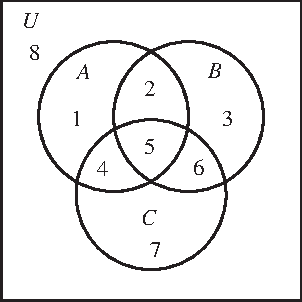
\includegraphics[width=\linewidth]{external/figps-venn3.pdf}
\end{image}%
 For the set \((A \cap B) \cap C\), region 5 is shaded.  %
\item[(ii)]\par\smallskip%
\noindent\hypertarget{g:solution:idm823762728-back}{}\begin{image}{0.3}{0.4}{0.3}%
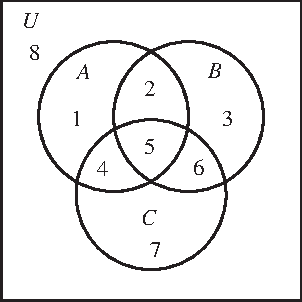
\includegraphics[width=\linewidth]{external/figps-venn3.pdf}
\end{image}%
 For the set \((A \cap B) \cup C\), the regions 2, 4, 5, 6, 7 are shaded.%
\item[(iii)]\par\smallskip%
\noindent\hypertarget{g:solution:idm823760168-back}{}\begin{image}{0.3}{0.4}{0.3}%
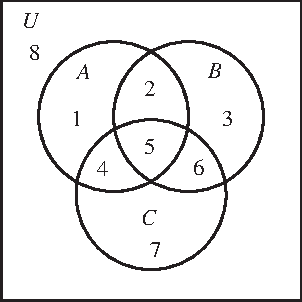
\includegraphics[width=\linewidth]{external/figps-venn3.pdf}
\end{image}%
 For the set \((A^c \cup B)\), the regions 2, 3, 5, 6, 7, 8 are shaded.%
\item[(iv)]\par\smallskip%
\noindent\hypertarget{g:solution:idm823751592-back}{}\begin{image}{0.3}{0.4}{0.3}%
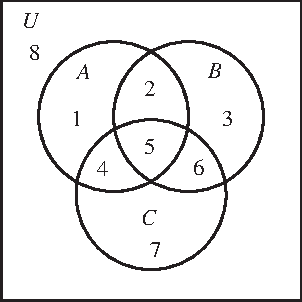
\includegraphics[width=\linewidth]{external/figps-venn3.pdf}
\end{image}%
 For the set \((A^c \cap (B \cup C))\), the regions 3, 6, 7 are shaded.%
\end{enumerate}
\item[(b)]\par\smallskip%
\noindent\hypertarget{g:solution:idm823754280-back}{}\begin{image}{0.3}{0.4}{0.3}%
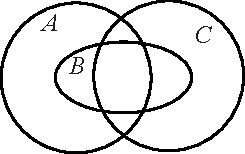
\includegraphics[width=\linewidth]{external/figps-prog54-2.pdf}
\end{image}%
%
\item[(c)]\par\smallskip%
\noindent\hypertarget{g:solution:idm823756072-back}{}\begin{image}{0.3}{0.4}{0.3}%
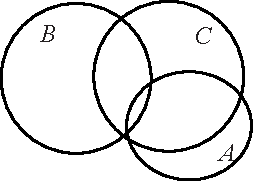
\includegraphics[width=\linewidth]{external/figps-prog54-3.pdf}
\end{image}%
%
\end{enumerate}
\end{inlinesolution}%
\par\medskip
\noindent\textbf{\Large{}5.2\space{}Proving Set Relationships\\
\space{}The Choose-an-Element Method}
\begin{inlinesolution}{5.13}{Subsets and Set Equality.}{x:exercise:prog_setequality}%
\begin{enumerate}[font=\bfseries,label=(\alph*),ref=\alph*]
\item[(a)]\par\smallskip%
\noindent\hypertarget{g:solution:idm823312408-back}{}The set \(A\) is a subset of \(B\). To prove this, we let \(x \in A\). Then there exists an integer \(m\) such that \(x = 9m\), which can be written as%
\begin{equation*}
x = 3 \left( 3m \right)\!\text{.}
\end{equation*}
Since \(3m \in \Z\), the last equation proves that \(x\) is a multiple of 3 and so \(x \in B\). Therefore, \(A \subseteq B\).%
\item[(b)]\par\smallskip%
\noindent\hypertarget{g:solution:idm823302040-back}{}The set \(A\) is not equal to the set \(B\). We note that \(3 \in B\) but \(3 \notin A\). Therefore, \(B \not \subseteq A\) and, hence, \(A \ne B\).%
\end{enumerate}
\end{inlinesolution}%
\begin{inlinesolution}{5.14}{Using the Choose-an-Element Method.}{x:exercise:prog_usingchoose}%
\begin{enumerate}[font=\bfseries,label=(\alph*),ref=\alph*]
\item[(b)]\par\smallskip%
\noindent\hypertarget{g:solution:idm823273624-back}{}\begin{center}%
{\tabularfont%
\begin{tabular}{lll}
\multicolumn{1}{lB}{Step}&\multicolumn{1}{lB}{Know}&Reason\tabularnewline\hrulethin
\multicolumn{1}{lB}{\(P\)}&\multicolumn{1}{lB}{\(A \subseteq B\)}&Hypothesis\tabularnewline\hrulemedium
\multicolumn{1}{lB}{\(P1\)}&\multicolumn{1}{lB}{Let \(x \in B^c\).}&\tablecelllines{l}{m}
{Choose an arbitrary element\\
of \(B^c\).}
\tabularnewline\hrulethin
\multicolumn{1}{lB}{\(P2\)}&\multicolumn{1}{lB}{If \(x \in A\), then \(x \in B\).}&Definition of ``subset''\tabularnewline\hrulethin
\multicolumn{1}{lB}{\(P3\)}&\multicolumn{1}{lB}{If \(x \notin B\), then \(x \notin A\).}&Contrapositive\tabularnewline\hrulemedium
\multicolumn{1}{lB}{\(P4\)}&\multicolumn{1}{lB}{If \(x \in B^c\), then \(x \in A^c\).}&\tablecelllines{l}{m}
{Step \(P3\) and definition\\
of ``complement''}
\tabularnewline\hrulemedium
\multicolumn{1}{lB}{\(Q2\)}&\multicolumn{1}{lB}{The element \(x\) is in \(A^c\).}&Steps \(P1\) and \(P4\)\tabularnewline\hrulemedium
\multicolumn{1}{lB}{\(Q1\)}&\multicolumn{1}{lB}{Every element of \(B^c\) is an element of \(A^c\).}&\tablecelllines{l}{m}
{The choose-an-element\\
method with Steps \(P1\) and \(Q2\)}
\tabularnewline\hrulemedium
\multicolumn{1}{lB}{\(Q\)}&\multicolumn{1}{lB}{\(B^c \subseteq A^c\)}&Definition of ``subset''
\end{tabular}
}%
\end{center}%
%
\end{enumerate}
\end{inlinesolution}%
\par\medskip
\noindent\textbf{\Large{}\space{}Proving Set Equality}
\begin{inlinesolution}{5.17}{Set Equality.}{x:exercise:prog_setequality2}%
\par\smallskip%
\noindent\hypertarget{g:solution:idm823232536-back}{}\begin{solutionproof}
Let \(A\) and \(B\) be subsets of some universal set. We will prove that \(A - B = A \cap B^c\) by proving that each set is a subset of the other set. We will first prove that \(A - B \subseteq A \cap B^c\). Let \(x \in A - B\). We then know that \(x \in A\) and \(x \notin B\). However, \(x \notin B\) implies that \(x \in B^c\). Hence, \(x \in A\) and \(x \in B^c\), which means that \(x \in A \cap B^c\). This proves that \(A - B \subseteq A \cap B^c\).%
\par
To prove that \(A \cap B^c \subseteq A - B\), we let \(y \in A \cap B^c\). This means that \(y \in A\) and \(y \in B^c\), and hence, \(y \in A\) and \(y \notin B\). Therefore, \(y \in A - B\) and this proves that \(A \cap B^c \subseteq A - B\). Since we have proved that each set is a subset of the other set, we have proved that \(A - B = A \cap B^c\).%
\end{solutionproof}
\end{inlinesolution}%
\par\medskip
\noindent\textbf{\Large{}\space{}Disjoint Sets}
\begin{inlinesolution}{5.21}{Proving Two Sets Are Disjoint.}{x:exercise:prog_disjointsets}%
\par\smallskip%
\noindent\hypertarget{g:solution:idm823186712-back}{}\begin{solutionproof}
Let \(A = \{ x \in \Z \mid x \equiv 3 \pmod 12 \}\) and \(B = \{ y \in \Z \mid y \equiv 2 \pmod 8 \}\). We will use a proof by contradiction to prove that \(A \cap B = \emptyset\). So we assume that \(A \cap B \ne \emptyset\) and let \(x \in A \cap B\). We can then conclude that \(x \equiv 3 \pmod 12\) and that \(y \equiv 2 \pmod 8\). This means that there exist integers \(m\) and \(n\) such that%
\begin{equation*}
x = 3 + 12m  \text{ and }   x = 2 + 8n\text{.}
\end{equation*}
%
\par
By equating these two expressions for \(x\), we obtain \(3 + 12m = 2 + 8n\), and this equation can be rewritten as \(1 = 8n - 12m\). This is a contradiction since 1 is an odd integer and \(8n - 12m\) is an even integer. We have therefore proved that \(A \cap B = \emptyset\).%
\end{solutionproof}
\end{inlinesolution}%
\par\medskip
\noindent\textbf{\Large{}5.3\space{}Properties of Set Operations\\
\space{}Proof of One of the Commutative Laws in Theorem~{\xreffont\ref*{x:theorem:T_algebraofsets}}}
\begin{inlinesolution}{5.25}{Exploring a Distributive Property.}{x:exercise:prog_workingvenn3}%
\begin{enumerate}[font=\bfseries,label=(\alph*),ref=\alph*]
\item[(a)]\par\smallskip%
\noindent\hypertarget{g:solution:idm822881704-back}{}In our standard configuration for a Venn diagram with three sets, regions 1, 2, 4, 5, and 6 are the shaded regions for both \(A \cup \left( {B \cap C} \right)\) and \(\left( {A \cup B} \right) \cap 
\left( {A \cup C} \right)\).%
\item[(b)]\par\smallskip%
\noindent\hypertarget{g:solution:idm822881192-back}{}Based on the Venn diagrams in Part (1), it appears that \(A \cup \left( {B \cap C} \right) = \left( {A \cup B} \right) 
\cap \left( {A \cup C} \right)\).%
\end{enumerate}
\end{inlinesolution}%
\par\medskip
\noindent\textbf{\Large{}\space{}Important Properties of Set Complements}
\begin{inlinesolution}{5.27}{}{x:exercise:A_usingalgebrasets1}%
\par\smallskip%
\noindent\hypertarget{g:solution:idm822831016-back}{}Using our standard configuration for a Venn diagram with three sets, regions 1, 2, and 3 are the regions that are shaded for both \(\left( {A \cup B} \right) - C\) and \(\left( {A - C} \right) \cup 
\left( {B - C} \right)\).%
\end{inlinesolution}%
\begin{inlinesolution}{5.28}{}{x:exercise:A_usingalgebrasets2}%
\par\smallskip%
\noindent\hypertarget{g:solution:idm822824360-back}{}%
\begin{align*}
\left( {A \cup B} \right) - C \amp = \left( {A \cup B} \right) \cap C^c \amp \hyperref[x:theorem:T_propsofcomplements]{\text{Theorem {\xreffont\ref{x:theorem:T_propsofcomplements}}, p.\,\pageref{x:theorem:T_propsofcomplements}}}\\
\amp = C^c  \cap \left( {A \cup B} \right) \amp \text{ (Commutative Property) }\\
\amp = \left( C^c \cap A \right) \cup \left( C^c \cap B \right) \amp \text{ Distributive Property }\\
\amp = \left( A \cap C^c \right) \cup \left( B \cap C^c \right) \amp \text{ (Commutative Property) }\\
\amp = \left( A - C \right) \cup \left( B - C \right) \amp \hyperref[x:theorem:T_propsofcomplements]{\text{Theorem {\xreffont\ref{x:theorem:T_propsofcomplements}}, p.\,\pageref{x:theorem:T_propsofcomplements}}}
\end{align*}
%
\end{inlinesolution}%
\par\medskip
\noindent\textbf{\Large{}5.4\space{}Cartesian Products\\
\space{}Cartesian Products}
\begin{inlinesolution}{5.30}{Relationships between Cartesian Products.}{x:exercise:prog_relationscartesian}%
\begin{enumerate}[font=\bfseries,label=(\alph*),ref=\alph*]
\item[(a)]\begin{enumerate}[font=\bfseries,label=(\roman*),ref=\theenumi.\roman*]
\item[(i)]\par\smallskip%
\noindent\hypertarget{g:solution:idm822549800-back}{}\(A \times B = \left\{ {\left( {1, a} \right), \left( {1, b} \right), 
\left( {2, a} \right), \left( {2, b} \right), \left( {3, a} \right), 
\left( {3, b} \right)} \right\}\)%
\item[(ii)]\par\smallskip%
\noindent\hypertarget{g:solution:idm822548264-back}{}\(T \times B = \left\{ {\left( {1, a} \right), \left( {1, b} \right), 
\left( {2, a} \right), \left( {2, b} \right)} \right\}\)%
\item[(iii)]\par\smallskip%
\noindent\hypertarget{g:solution:idm822547368-back}{}\(A \times C = \left\{ {\left( {1, a} \right), \left( {1, c} \right), 
\left( {2, a} \right), \left( {2, c} \right), \left( {3, a} \right), 
\left( {3, c} \right)} \right\}\)%
\item[(iv)]\par\smallskip%
\noindent\hypertarget{g:solution:idm822546600-back}{}\(A \times \left( {B \cap C} \right) = \left\{ {\left( {1, a} \right), 
\left( {2, a} \right), \left( {3, a} \right)} \right\}\)%
\item[(v)]\par\smallskip%
\noindent\hypertarget{g:solution:idm822543144-back}{}\(\left( {A \times B} \right) \cap \left( {A \times C} \right) = 
\left\{ {\left( {1, a} \right), \left( {2, a} \right), \left( {3, a} \right)} \right\}\)%
\item[(vi)]\par\smallskip%
\noindent\hypertarget{g:solution:idm822543656-back}{}\(A \times \left( {B \cup C} \right) = \left\{ {\left( {1, a} \right), 
\left( {1, b} \right), \left( {1, c} \right), \left( {2, a} \right), 
\left( {2, b} \right), \left( {2, c} \right), \left( {3, a} \right), \left( {3, b} \right), \left( {3, c} \right)} \right\}\)%
\item[(vii)]\par\smallskip%
\noindent\hypertarget{g:solution:idm822537256-back}{}\(\left( {A \times B} \right) \cup \left( {A \times C} \right) = 
\left\{ {\left( {1, a} \right), \left( {1, b} \right), \left( {1, c} \right), 
\left( {2, a} \right), \left( {2, b} \right), \left( {2, c} \right), \left( {3, a} \right), 
\left( {3, b} \right), \left( {3, c} \right)} \right\}\)%
\item[(viii)]\par\smallskip%
\noindent\hypertarget{g:solution:idm822542888-back}{}\(A \times \left( {B - C} \right) = \left\{ {\left( {1, b} \right), 
\left( {2, b} \right), \left( {3, b} \right)} \right\}\)%
\item[(ix)]\par\smallskip%
\noindent\hypertarget{g:solution:idm822538664-back}{}\(\left( {A \times B} \right) - \left( {A \times C} \right) = 
\left\{ {\left( {1, b} \right), \left( {2, b} \right), \left( {3, b} \right)} 
\right\}\)%
\item[(x)]\par\smallskip%
\noindent\hypertarget{g:solution:idm822535208-back}{}\(B \times A = \left\{ {\left( {a, 1} \right), \left( {b, 1} \right), 
\left( {a, 2} \right), \left( {b, 2} \right), \left( {a, 3} \right), 
\left( {b, 3} \right)} \right\}\)%
\end{enumerate}
\item[(b)]\par\smallskip%
\noindent\hypertarget{g:solution:idm822533928-back}{}\(T \times B \subseteq A \times B\)%
\par
\(A \times \left( {B \cap C} \right) = \left( {A \times B} \right) \cap 
\left( {A \times C} \right)\)%
\par
\(A \times \left( {B \cup C} \right) = \left( {A \times B} \right) \cup 
\left( {A \times C} \right)\)%
\par
\(A \times \left( {B - C} \right) = \left( {A \times B} \right) - 
\left( {A \times C} \right)\)%
\end{enumerate}
\end{inlinesolution}%
\par\medskip
\noindent\textbf{\Large{}\space{}The Cartesian Plane}
\begin{inlinesolution}{5.32}{Cartesian Products of Intervals.}{x:exercise:prog_cartprodintervals}%
\begin{enumerate}[font=\bfseries,label=(\alph*),ref=\alph*]
\item[(a)]\begin{enumerate}[font=\bfseries,label=(\roman*),ref=\theenumi.\roman*]
\item[(i)]\par\smallskip%
\noindent\hypertarget{g:solution:idm822506280-back}{}\(A \times B = \left\{ {\left( {x,y} \right) \in \mathbb{R} \times \mathbb{R} 
\mid {0 \leq x \leq 2\text{ and } 2 \leq y \lt 4} } \right\}\)%
\item[(ii)]\par\smallskip%
\noindent\hypertarget{g:solution:idm822504232-back}{}\(T \times B = \left\{ {\left( {x,y} \right) \in \mathbb{R} \times 
\mathbb{R} \mid {1 \lt x \lt 2\text{ and } 2 \leq y \lt 4} } \right\}\)%
\item[(iii)]\par\smallskip%
\noindent\hypertarget{g:solution:idm822508840-back}{}\(A \times C = \left\{ {\left( {x,y} \right) \in \mathbb{R} \times 
\mathbb{R} \mid {0 \leq x \leq 2\text{ and } 3 \lt y \leq 5} } \right\}\)%
\item[(iv)]\par\smallskip%
\noindent\hypertarget{g:solution:idm822499368-back}{}\(A \times \left( {B \cap C} \right) = \left\{ {\left( {x,y} \right) \in 
\mathbb{R} \times \mathbb{R} \mid {0 \leq x \leq 2\text{ and } 3 \lt y \lt 4} } 
\right\}\)%
\item[(v)]\par\smallskip%
\noindent\hypertarget{g:solution:idm822502184-back}{}\(\left( {A \times B} \right) \cap \left( {A \times C} \right) = 
\left\{ {\left( {x,y} \right) \in \mathbb{R} \times \mathbb{R} 
\mid {0 \leq x \leq 2\text{ and } 3 \lt y \lt 4} } \right\}\)%
\item[(vi)]\par\smallskip%
\noindent\hypertarget{g:solution:idm822496424-back}{}\(A \times \left( {B \cup C} \right) = \left\{ {\left( {x,y} \right) \in 
\mathbb{R} \times \mathbb{R} \mid {0 \leq x \leq 2\text{ and 2 } \leq y \leq 5} } \right\}\)%
\item[(vii)]\par\smallskip%
\noindent\hypertarget{g:solution:idm822495912-back}{}\(\left( {A \times B} \right) \cup \left( {A \times C} \right) = 
\left\{ {\left( {x,y} \right) \in \mathbb{R} \times \mathbb{R} 
\mid {0 \leq x \leq 2\text{ and 2 } \leq y \leq 5} } \right\}\)%
\item[(viii)]\par\smallskip%
\noindent\hypertarget{g:solution:idm822501032-back}{}\(A \times \left( {B - C} \right) = \left\{ {\left( {x,y} \right) \in 
\mathbb{R} \times \mathbb{R} \mid {0 \leq x \leq 2\text{ and } 2 \leq y \leq 3} } \right\}\)%
\item[(ix)]\par\smallskip%
\noindent\hypertarget{g:solution:idm822491560-back}{}\(\left( {A \times B} \right) - \left( {A \times C} \right) = 
\left\{ {\left( {x,y} \right) \in \mathbb{R} \times \mathbb{R} \mid {0 \leq x 
\leq 2\text{ and } 2 \leq y \leq 3} } \right\}\)%
\item[(x)]\par\smallskip%
\noindent\hypertarget{g:solution:idm822492200-back}{}\(B \times A = \left\{ {\left( {x,y} \right) \in \mathbb{R} \times 
\mathbb{R} \mid {2 \leq x \lt 4 \text{ and } 0 \leq y \leq 2} } \right\}\)%
\end{enumerate}
\item[(b)]\par\smallskip%
\noindent\hypertarget{g:solution:idm822492072-back}{}\(T \times B \subseteq A \times B\)%
\par
\(A \times \left( {B \cap C} \right) = 
\left( {A \times B} \right) \cap \left( {A \times C} \right)\)%
\par
\(A \times \left( {B \cup C} \right) = \left( {A \times B} \right) \cup 
\left( {A \times C} \right)\)%
\par
\(A \times \left( {B - C} \right) = 
\left( {A \times B} \right) - \left( {A \times C} \right)\)%
\end{enumerate}
\end{inlinesolution}%
\par\medskip
\noindent\textbf{\Large{}5.5\space{}Indexed Families of Sets\\
\space{}The Union and Intersection of an Indexed Family of Sets}
\begin{inlinesolution}{5.35}{An Infinite Family of Sets.}{x:exercise:prog_infinitefamily}%
\begin{enumerate}[font=\bfseries,label=(\alph*),ref=\alph*]
\item[(a)]\par\smallskip%
\noindent\hypertarget{g:solution:idm822247592-back}{}\(\bigcup\limits_{j=1}^{6}A_j = \{1, 2, 3, 4, 5, 6, 9, 16, 25, 36 \}\)%
\item[(b)]\par\smallskip%
\noindent\hypertarget{g:solution:idm822236712-back}{}\(\bigcap\limits_{j=1}^{6}A_j = \{ 1 \}\)%
\item[(c)]\par\smallskip%
\noindent\hypertarget{g:solution:idm822233000-back}{}\(\bigcup\limits_{j=3}^{6}A_j = \{3, 4, 5, 6, 9, 16, 25, 36 \}\)%
\item[(d)]\par\smallskip%
\noindent\hypertarget{g:solution:idm822233768-back}{}\(\bigcap\limits_{j=3}^{6}A_j = \{ 1 \}\)%
\item[(e)]\par\smallskip%
\noindent\hypertarget{g:solution:idm822240936-back}{}\(\bigcup\limits_{j=1}^{\infty}A_j = \N\)%
\item[(f)]\par\smallskip%
\noindent\hypertarget{g:solution:idm822235560-back}{}\(\bigcap\limits_{j=1}^{\infty}A_j = \{ 1 \}\)%
\end{enumerate}
\end{inlinesolution}%
\begin{inlinesolution}{5.36}{Indexed Families of Sets.}{x:exercise:prog_indexfamily}%
\begin{enumerate}[font=\bfseries,label=(\alph*),ref=\alph*]
\item[(a)]\par\smallskip%
\noindent\hypertarget{g:solution:idm822213160-back}{}\(A_1 = \{7, 14 \}, A_2 = \{10, 12 \}, A_3 = \{10, 12 \}, A_4 = \{8, 14 \}\).%
\item[(b)]\par\smallskip%
\noindent\hypertarget{g:solution:idm822214824-back}{}The statement is false. For example, \(2 \ne 3\) and \(A_2 = A_3\).%
\item[(c)]\par\smallskip%
\noindent\hypertarget{g:solution:idm822205864-back}{}The statement is false. For example, \(1 \ne -1\) and \(B_1 = B_{-1}\).%
\end{enumerate}
\end{inlinesolution}%
\begin{inlinesolution}{5.38}{A Continuation of Example~{\xreffont\ref*{x:example:exam_indexfamily}}.}{x:exercise:prog_indexfamily2}%
\begin{enumerate}[font=\bfseries,label=(\alph*),ref=\alph*]
\item[(a)]\par\smallskip%
\noindent\hypertarget{g:solution:idm822176168-back}{}Since \(\bigcup\limits_{\alpha \in \R^+}^{}A_\alpha = \left( -1, \infty \right)\), \(\left( \bigcup\limits_{\alpha \in \R^+}^{}A_\alpha \right)^c = (-\infty, 1 ]\).%
\item[(b)]\par\smallskip%
\noindent\hypertarget{g:solution:idm822172584-back}{}\(\bigcap\limits_{\alpha \in \R^+}^{}A_{\alpha}^c = (-\infty, -1]\).%
\item[(c)]\par\smallskip%
\noindent\hypertarget{g:solution:idm822172328-back}{}Since \(\bigcap\limits_{\alpha \in \R^+}^{}A_\alpha = \left( -1, 0 \right]\), \(\left( \bigcap\limits_{\alpha \in \R^+}^{}A_\alpha \right)^c = (-\infty, -1] 
\cup (0, \infty)\).%
\item[(d)]\par\smallskip%
\noindent\hypertarget{g:solution:idm822170664-back}{}\(\bigcup\limits_{\alpha \in \R^+}^{}A_{\alpha}^c = (-\infty, -1] \cup (0, \infty)\).%
\end{enumerate}
\end{inlinesolution}%
\par\medskip
\noindent\textbf{\Large{}\space{}Pairwise Disjoint Families of Sets}
\begin{inlinesolution}{5.41}{Disjoint Families of Sets.}{x:exercise:prog_disjoint}%
\begin{enumerate}[font=\bfseries,label=(\alph*),ref=\alph*]
\item[(c)]\par\smallskip%
\noindent\hypertarget{g:solution:idm822117144-back}{}All three families of sets \(\left( \mathscr{A}, \mathscr{B}, \text{ and } \mathscr{C} \right)\) are disjoint families of sets. Only the family \(\mathscr{A}\) is a pairwise disjoint family of sets.%
\end{enumerate}
\end{inlinesolution}%
\par\medskip
\noindent\textbf{\Large{}6\space{}Functions\\
6.1\space{}Introduction to Functions\\
\space{}The Definition of a Function}
\begin{inlinesolution}{6.1}{Images and Preimages.}{x:exercise:pr_images}%
\begin{enumerate}[font=\bfseries,label=(\alph*),ref=\alph*]
\item[(a)]\par\smallskip%
\noindent\hypertarget{g:solution:idm821706776-back}{}\(f ( -3 ) = 24\) \(f ( \sqrt{8} ) = 8 - 5 \sqrt{8}\)%
\item[(b)]\par\smallskip%
\noindent\hypertarget{g:solution:idm821703576-back}{}\(g ( 2 ) = -6\), \(g ( -2 ) = 14\)%
\item[(c)]\par\smallskip%
\noindent\hypertarget{g:solution:idm821693720-back}{}\(\left\{ -1, 6 \right\}\)%
\item[(d)]\par\smallskip%
\noindent\hypertarget{g:solution:idm821698328-back}{}\(\left\{ -1, 6 \right\}\)%
\item[(e)]\par\smallskip%
\noindent\hypertarget{g:solution:idm821696536-back}{}\(\left\{ \dfrac{5 + \sqrt{33}}{2}, \dfrac{5 - \sqrt{33}}{2} \right\}\)%
\item[(f)]\par\smallskip%
\noindent\hypertarget{g:solution:idm821696152-back}{}\(\emptyset\)%
\end{enumerate}
\end{inlinesolution}%
\par\medskip
\noindent\textbf{\Large{}\space{}The Codomain and Range of a Function}
\begin{inlinesolution}{6.2}{Codomain and Range.}{x:exercise:pr_codomainandrange1}%
\begin{enumerate}[font=\bfseries,label=(\alph*),ref=\alph*]
\item[(a)]\begin{enumerate}[font=\bfseries,label=(\roman*),ref=\theenumi.\roman*]
\item[(i)]\par\smallskip%
\noindent\hypertarget{g:solution:idm821681816-back}{}The domain of the function \(f\) is the set of all people.%
\item[(ii)]\par\smallskip%
\noindent\hypertarget{g:solution:idm821676696-back}{}A codomain for the function \(f\) is the set of all days in a leap year.%
\item[(iii)]\par\smallskip%
\noindent\hypertarget{g:solution:idm821674648-back}{}This means that the range of the function \(f\) is equal to its codomain.%
\end{enumerate}
\item[(b)]\begin{enumerate}[font=\bfseries,label=(\roman*),ref=\theenumi.\roman*]
\item[(i)]\par\smallskip%
\noindent\hypertarget{g:solution:idm821671576-back}{}The domain of the function \(s\) is the set of natural numbers.%
\item[(ii)]\par\smallskip%
\noindent\hypertarget{g:solution:idm821670936-back}{}A codomain for the function \(s\) is the set of natural numbers.%
\item[(iii)]\par\smallskip%
\noindent\hypertarget{g:solution:idm821659928-back}{}This means that the range of \(s\) is not equal to the set of natural numbers.%
\end{enumerate}
\end{enumerate}
\end{inlinesolution}%
\par\medskip
\noindent\textbf{\Large{}\space{}The Graph of a Real Function}
\begin{inlinesolution}{6.4}{Using the Graph of a Real Function.}{x:exercise:pr_graphreal}%
\begin{enumerate}[font=\bfseries,label=(\alph*),ref=\alph*]
\item[(a)]\par\smallskip%
\noindent\hypertarget{g:solution:idm821643032-back}{}\(f(-1) \approx -3\) and \(f(2) \approx -2.5\).%
\item[(b)]\par\smallskip%
\noindent\hypertarget{g:solution:idm821646360-back}{}Values of \(x\) for which \(f(x) = 2\) are approximately \(-2.8, -1.9, 0.3, 1.2\), and 3.5.%
\item[(c)]\par\smallskip%
\noindent\hypertarget{g:solution:idm821637144-back}{}The range of \(f\) appears to be the closed interval \([-3.2, 3.2]\) or \(\{ y \in \R \mid -3.2 \leq y \leq 3.2 \}\).%
\end{enumerate}
\end{inlinesolution}%
\par\medskip
\noindent\textbf{\Large{}\space{}Arrow Diagrams}
\begin{inlinesolution}{6.7}{Working with Arrow Diagrams.}{x:exercise:pr_arrow}%
\begin{enumerate}[font=\bfseries,label=(\alph*),ref=\alph*]
\item[(b)]\par\smallskip%
\noindent\hypertarget{g:solution:idm821634712-back}{}Only the arrow diagram in Figure~(a) can be used to represent a function from \(A\) to \(B\). The range of this function is the set \(\{ a, b \}\).%
\end{enumerate}
\end{inlinesolution}%
\par\medskip
\noindent\textbf{\Large{}6.2\space{}More about Functions\\
\space{}Functions Involving Congruences}
\begin{inlinesolution}{6.10}{Functions Defined by Congruences.}{x:exercise:pr_congfunctions}%
\begin{enumerate}[font=\bfseries,label=(\alph*),ref=\alph*]
\item[(a)]\par\smallskip%
\noindent\hypertarget{g:solution:idm821724056-back}{}\(f(0) = 0\), \(f(1) = 1\), \(f(2) = 1\), \(f(3) = 1\), \(f(4) = 1\).%
\item[(b)]\par\smallskip%
\noindent\hypertarget{g:solution:idm821364504-back}{}\(g(0) = 0\), \(g(1) = 1\), \(g(2) = 2\), \(g(3) = 3\), \(g(4) = 4\).%
\end{enumerate}
\end{inlinesolution}%
\par\medskip
\noindent\textbf{\Large{}\space{}Equality of Functions}
\begin{inlinesolution}{6.11}{Equality of Functions.}{x:exercise:pr_equalfunc}%
\par\smallskip%
\noindent\hypertarget{g:solution:idm821336600-back}{}\(I_{\Z_5} \ne f\) and \(I_{\Z_5} = g\).%
\end{inlinesolution}%
\par\medskip
\noindent\textbf{\Large{}\space{}Mathematical Processes as Functions}
\begin{inlinesolution}{6.12}{Average of a Finite Set of Numbers.}{x:exercise:pr_average}%
\begin{enumerate}[font=\bfseries,label=(\alph*),ref=\alph*]
\item[(a)]\par\smallskip%
\noindent\hypertarget{g:solution:idm821322264-back}{}3.5%
\item[(b)]\par\smallskip%
\noindent\hypertarget{g:solution:idm821319320-back}{}4.02%
\item[(c)]\par\smallskip%
\noindent\hypertarget{g:solution:idm821322136-back}{}\(\dfrac{\pi + \sqrt{2}}{4}\)%
\item[(d)]\par\smallskip%
\noindent\hypertarget{g:solution:idm821314712-back}{}The process of finding the average of a finite set of real numbers can be thought of as a function from \(\mathcal{F} ( \R )\) to \(\R\). So the domain is \(\mathcal{F} ( \R )\), the codomain is \(\R\), and we can define a function \(\text{ avg } : \mathcal{F} ( \R ) \to \R\) as follows: If \(A \in \mathscr{F} ( \R )\) and \(A = \left\{ a_1, a_2, \ldots,
a_n \right\}\), then \(\text{ avg } ( A ) = \dfrac{a_1 + a_2 + \cdots + a_n}{n}\).%
\end{enumerate}
\end{inlinesolution}%
\par\medskip
\noindent\textbf{\Large{}\space{}Sequences as Functions}
\begin{inlinesolution}{6.13}{Sequences.}{x:exercise:pr_sequences}%
\begin{enumerate}[font=\bfseries,label=(\alph*),ref=\alph*]
\item[(a)]\par\smallskip%
\noindent\hypertarget{g:solution:idm821298072-back}{}The sixth term is \(\dfrac{1}{18}\) and the tenth term is \(\dfrac{1}{30}\).%
\item[(b)]\par\smallskip%
\noindent\hypertarget{g:solution:idm821296152-back}{}The sixth term is \(\dfrac{1}{36}\) and the tenth term is \(\dfrac{1}{100}\).%
\item[(c)]\par\smallskip%
\noindent\hypertarget{g:solution:idm821297304-back}{}The sixth term is \(1\) and the tenth term is \(1\).%
\end{enumerate}
\end{inlinesolution}%
\par\medskip
\noindent\textbf{\Large{}\space{}Functions of Two Variables}
\begin{inlinesolution}{6.14}{Working with a Function of Two Variables.}{x:exercise:pr_function-two}%
\begin{enumerate}[font=\bfseries,label=(\alph*),ref=\alph*]
\item[(a)]\par\smallskip%
\noindent\hypertarget{g:solution:idm821273368-back}{}\(g ( 0, 3 ) = -3\); \(g ( 3, -2 ) = 11\); \(g ( -3, -2 ) = 11\); \(g ( 7, -1 ) = 50\).%
\item[(b)]\par\smallskip%
\noindent\hypertarget{g:solution:idm821274264-back}{}\(\left\{ (m, n) \in \Z \times \Z \mid n = m^2 \right\}\)%
\item[(c)]\par\smallskip%
\noindent\hypertarget{g:solution:idm821268760-back}{}\(\left\{ (m, n) \in \Z \times \Z \mid n = m^2 - 5 \right\}\)%
\end{enumerate}
\end{inlinesolution}%
\par\medskip
\noindent\textbf{\Large{}6.3\space{}Injections, Surjections, and Bijections\\
\space{}Injections}
\begin{inlinesolution}{6.16}{Working with the Definition of an Injection.}{x:exercise:pr_injections}%
\begin{enumerate}[font=\bfseries,label=(\alph*),ref=\alph*]
\item[(e)]\par\smallskip%
\noindent\hypertarget{g:solution:idm820901784-back}{}The functions \(k\), \(F\), and \(s\) are injections. The functions \(f\) and \(h\) are not injections.%
\end{enumerate}
\end{inlinesolution}%
\par\medskip
\noindent\textbf{\Large{}\space{}Surjections}
\begin{inlinesolution}{6.17}{Working with the Definition of a Surjection.}{x:exercise:pr_functionswithfinitedom}%
\begin{enumerate}[font=\bfseries,label=(\alph*),ref=\alph*]
\item[(d)]\par\smallskip%
\noindent\hypertarget{g:solution:idm820855192-back}{}The functions \(f\) and \(s\) are surjections. The functions \(k\) and \(F\) are not surjections.%
\end{enumerate}
\end{inlinesolution}%
\par\medskip
\noindent\textbf{\Large{}\space{}The Importance of the Domain and Codomain}
\begin{inlinesolution}{6.21}{The Importance of the Domain and Codomain.}{x:exercise:pr_domainandcodomain}%
\par\smallskip%
\noindent\hypertarget{g:solution:idm820797592-back}{}The function \(f\) is an injection but not a surjection. To see that it is an injection, let \(a, b \in \R\) and assume that \(f(a) = f(b)\). This implies that \(e^{-a} = e^{-b}\). Now use the natural logarithm function to prove that \(a = b\). Since \(e^{-x} > 0\) for each real number \(x\), there is no \(x \in \R\) such that \(f(x) = -1\). So \(f\) is not a surjection.%
\par
The function \(g\) is an injection and is a surjection. The proof that \(g\) is an injection is basically the same as the proof that \(f\) is an injection. To prove that \(g\) is a surjection, let \(b \in \R^+\). To construct the real number \(a\) such that \(g(a) = b\), solve the equation \(e^{-a} = b\) for \(a\). The solution is \(a = -\ln b\). It can then be verified that \(g(a) = b\).%
\end{inlinesolution}%
\par\medskip
\noindent\textbf{\Large{}\space{}Working with a Function of Two Variables}
\begin{inlinesolution}{6.22}{A Function of Two Variables.}{x:exercise:pr_function2variables}%
\begin{enumerate}[font=\bfseries,label=(\alph*),ref=\alph*]
\item[(a)]\par\smallskip%
\noindent\hypertarget{g:solution:idm820764952-back}{}There are several ordered pairs \((a, b) \in \R \times \R\) such that \(g(a, b) = 2\). For example, \(g(0, 2) = 2\), \(g(-1, 4) = 2\), and \(g(2, -2) = 2\).%
\item[(b)]\par\smallskip%
\noindent\hypertarget{g:solution:idm820750360-back}{}For each \(z \in \R\), \(g(0, z) = z\).%
\item[(c)]\par\smallskip%
\noindent\hypertarget{g:solution:idm820754968-back}{}Part~(1) implies that the function \(g\) is not an injection. Part~(2) implies that the function \(g\) is a surjection since for each \(z \in \R\), \((0, z)\) is in the domain of \(g\) and \(g(0, z) = z\).%
\end{enumerate}
\end{inlinesolution}%
\par\medskip
\noindent\textbf{\Large{}6.4\space{}Composition of Functions\\
\space{}Composition and Arrow Diagrams}
\begin{inlinesolution}{6.26}{The Composition of Two Functions.}{x:exercise:pr_compose}%
\par\smallskip%
\noindent\hypertarget{g:solution:idm820517160-back}{}The arrow diagram for \(g \circ f: A \to B\) should show the following:%
\begin{align*}
(g \circ f)(a) \amp = g(f(a)) \amp   (g \circ f)(b) \amp = g(f(b))\\
\amp = g(2) = 1 \amp                 \amp = g(3) = 2\\
(g \circ f)(c) \amp = g(f(c)) \amp   (g \circ f)(d) \amp = g(f(d))\\
\amp = g(1) = 3 \amp                 \amp = g(2) = 1
\end{align*}
%
\par
The arrow diagram for \(g \circ g: B \to B\) should show the following:%
\begin{align*}
(g \circ g)(1) \amp = g(g(1)) \amp   (g \circ g)(2) \amp = g(g(2))\\
\amp = g(3) = 2 \amp                 \amp = g(1) = 3\\
(g \circ g)(3) \amp = g(g(3))\\
\amp = g(2) = 1
\end{align*}
%
\end{inlinesolution}%
\par\medskip
\noindent\textbf{\Large{}\space{}Decomposing Functions}
\begin{inlinesolution}{6.27}{Decomposing Functions.}{x:exercise:prog_decompose}%
\begin{enumerate}[font=\bfseries,label=(\alph*),ref=\alph*]
\item[(a)]\par\smallskip%
\noindent\hypertarget{g:solution:idm820502696-back}{}\(F = g \circ f\), where \(f:\R \to \R\) by \(f ( x ) = x^2 + 3\), and \(g:\R \to \R\) by \(g(x) = x^3\).%
\item[(b)]\par\smallskip%
\noindent\hypertarget{g:solution:idm820489256-back}{}\(G = h \circ f\), where \(f:\R \to \R^+\) by \(f( x ) = x^2 + 3\), and \(h:\R^+ \to \R\) by \(h(x) = \ln x\).%
\item[(c)]\par\smallskip%
\noindent\hypertarget{g:solution:idm820491560-back}{}\(f = g \circ k\), where \(k:\R \to \R\) by \(k(x) = x^2 - 3\) and \(g:\R \to \R\) by \(g(x) = |x|\).%
\item[(d)]\par\smallskip%
\noindent\hypertarget{g:solution:idm820488616-back}{}\(g = h \circ f\), where \(f:\R \to \R\) by \(f(x) = \dfrac{2x-3}{x^2 + 1}\) and \(h:\R \to \R\) by \(h(x) = \cos x\).%
\end{enumerate}
\end{inlinesolution}%
\par\medskip
\noindent\textbf{\Large{}\space{}Theorems about Composite Functions}
\begin{inlinesolution}{6.28}{Compositions of Injections and Surjections.}{x:exercise:prog_compositesofinjections}%
\begin{enumerate}[font=\bfseries,label=(\alph*),ref=\alph*]
\item[(a)]\par\smallskip%
\noindent\hypertarget{g:solution:idm820479272-back}{}\(g \circ f\) should be an injection.%
\item[(c)]\par\smallskip%
\noindent\hypertarget{g:solution:idm820471592-back}{}\(g \circ f\) should be a bijection.%
\end{enumerate}
\end{inlinesolution}%
\par\medskip
\noindent\textbf{\Large{}6.5\space{}Inverse Functions\\
\space{}The Ordered Pair Representation of a Function}
\begin{inlinesolution}{6.32}{Sets of Ordered Pairs that Are Not Functions.}{x:exercise:prog_ordered}%
\begin{enumerate}[font=\bfseries,label=(\alph*),ref=\alph*]
\item[(a)]\par\smallskip%
\noindent\hypertarget{g:solution:idm820089896-back}{}The set \(F\) does not satisfy the first condition of \hyperref[x:theorem:T_functionasordered]{Theorem~{\xreffont\ref{x:theorem:T_functionasordered}}, p.\,\pageref{x:theorem:T_functionasordered}}.%
\item[(b)]\par\smallskip%
\noindent\hypertarget{g:solution:idm820090408-back}{}The set \(G\) does not satisfy the second condition of \hyperref[x:theorem:T_functionasordered]{Theorem~{\xreffont\ref{x:theorem:T_functionasordered}}, p.\,\pageref{x:theorem:T_functionasordered}}.%
\end{enumerate}
\end{inlinesolution}%
\par\medskip
\noindent\textbf{\Large{}\space{}The Inverse of a Function}
\begin{inlinesolution}{6.33}{Exploring the Inverse of a Function.}{x:exercise:prog_exploringinverse}%
\begin{enumerate}[font=\bfseries,label=(\alph*),ref=\alph*]
\item[(b)]\par\smallskip%
\noindent\hypertarget{g:solution:idm820058536-back}{}\(f^{ - 1} = \left\{ {( {r, a} ), ( {p, b} ), ( {q, c} )} \right\}\)%
\par
\(g^{ - 1} = \left\{ {( {p, a} ), ( {q, b} ), ( {p, c} )} \right\}\)%
\par
\(h^{ - 1} = \left\{ {( {p, a} ), ( {q, b} ), ( {r, c} ), ( {q, d} )} \right\}\)%
\item[(c)]\begin{enumerate}[font=\bfseries,label=(\roman*),ref=\theenumi.\roman*]
\item[(i)]\par\smallskip%
\noindent\hypertarget{g:solution:idm820060712-back}{}\(f^{ - 1}\) is a function from \(C\) to \(A\).%
\item[(ii)]\par\smallskip%
\noindent\hypertarget{g:solution:idm820048552-back}{}\(g^{ - 1}\) is not a function from \(C\) to \(A\) since \(( {p, a} ) \in g^{ - 1}\)and \(( {p, c} ) \in g^{ - 1}\).%
\item[(iii)]\par\smallskip%
\noindent\hypertarget{g:solution:idm820049320-back}{}\(h^{ - 1}\) is not a function from \(C\) to \(B\) since \(( {q, b} ) \in h^{ - 1}\) and \(( {q, d} ) \in h^{ - 1}\).%
\end{enumerate}
\item[(e)]\par\smallskip%
\noindent\hypertarget{g:solution:idm820039080-back}{}In order for the inverse of a function \(F:S \to T\) to be a function from \(T\) to \(S\), the function \(F\) must be a bijection.%
\end{enumerate}
\end{inlinesolution}%
\par\medskip
\noindent\textbf{\Large{}6.6\space{}Functions Acting on Sets\\
\space{}Functions Acting on Sets}
\begin{inlinesolution}{6.42}{Beginning Activity 1 Revisited.}{x:exercise:prog_functionsandsets}%
\begin{enumerate}[font=\bfseries,label=(\alph*),ref=\alph*]
\item[(a)]\par\smallskip%
\noindent\hypertarget{g:solution:idm819663128-back}{}\(f ( A ) = \left\{ s, t \right\}\)%
\item[(b)]\par\smallskip%
\noindent\hypertarget{g:solution:idm819656984-back}{}\(f ( B ) = \left\{ f ( x ) \mid x \in B \right\} = \left\{ s \right\}\)%
\item[(c)]\par\smallskip%
\noindent\hypertarget{g:solution:idm819654168-back}{}\(f^{-1} ( C ) = \left\{ x \in S \mid f ( x ) \in C \right\} = 
\left\{ a, b, c, d \right\}\)%
\item[(d)]\par\smallskip%
\noindent\hypertarget{g:solution:idm819653144-back}{}\(f^{-1} ( D ) = \left\{ x \in S \mid f ( x ) \in D \right\} = \left\{ a, d \right\}\)%
\end{enumerate}
\end{inlinesolution}%
\par\medskip
\noindent\textbf{\Large{}\space{}Set Operations and Functions Acting on Sets}
\begin{inlinesolution}{6.44}{Set Operations and Functions Acting on Sets.}{x:exercise:prog_setsandfunctions}%
\begin{enumerate}[font=\bfseries,label=(\alph*),ref=\alph*]
\item[(a)]\par\smallskip%
\noindent\hypertarget{g:solution:idm819611288-back}{}%
\begin{align*}
f ( 0 ) = 2 \amp \amp f ( 2 ) = 6 \amp \amp f ( 4 ) = 2 \amp \amp f ( 7 ) = 3\\
f ( 1 ) = 3 \amp \amp f ( 3 ) = 3 \amp \amp f ( 5 ) = 3 \amp \amp f ( 6 ) = 6
\end{align*}
%
\item[(b)]\par\smallskip%
\noindent\hypertarget{g:solution:idm819605016-back}{}\(\) \(\) \(\) \(\)%
\begin{align*}
f ( A ) = \left\{ 2, 3, 6 \right\} \amp \amp f ( B ) = \left\{ 2, 3, 6 \right\}\\
f^{-1} ( C ) = \left\{ 0, 1, 3, 4, 5, 7 \right\} \amp \amp f^{-1} ( D ) = \left\{ 1, 3, 5, 7 \right\}
\end{align*}
%
\item[(c)]\begin{enumerate}[font=\bfseries,label=(\roman*),ref=\theenumi.\roman*]
\item[(i)]\par\smallskip%
\noindent\hypertarget{g:solution:idm819601304-back}{}\(f ( A \cap B ) = \left\{ 2 \right\}\) and \(f ( A ) \cap f ( B ) = 
\left\{ 2, 3, 6 \right\}\). So in this case, \(f ( A \cap B ) \subseteq f ( A ) \cap f ( B )\).%
\item[(ii)]\par\smallskip%
\noindent\hypertarget{g:solution:idm819596056-back}{}\(f ( A ) \cup f ( B ) = \left\{ 2, 3, 6 \right\}\) and \(f ( A \cup B ) = \left\{ 2, 3, 6 \right\}\). So in this case, \(f ( A \cup B ) = f ( A ) \cup f ( B )\).%
\item[(iii)]\par\smallskip%
\noindent\hypertarget{g:solution:idm819589400-back}{}\(f^{-1} ( C ) \cap f^{-1} ( D ) = f^{-1} ( C \cap D ) = 
\left\{ 1, 3, 5, 7 \right\}\). So in this case, \(f^{-1} ( C \cap D ) = f^{-1} ( C ) \cap f^{-1} ( D )\).%
\item[(iv)]\par\smallskip%
\noindent\hypertarget{g:solution:idm819591320-back}{}\(f^{-1} ( C ) \cup f^{-1} ( D ) = f^{-1} ( C \cup D ) = 
\left\{ 0, 1, 3, 4, 5, 7 \right\}\). So in this case, \(f^{-1} ( C \cup D ) = f^{-1} ( C ) \cup f^{-1} ( D )\).%
\end{enumerate}
\item[(d)]\par\smallskip%
\noindent\hypertarget{g:solution:idm819593496-back}{}\(f ( A ) = \left\{ 2, 3, 6 \right\}\). Hence, \(f^{-1} \!\left( f ( A ) \right) = \left\{ 0, 1, 2, 3, 4, 5, 6, 7 \right\}\). So in this case, \(A \subseteq f^{-1} \!\left( f ( A ) \right)\).%
\item[(e)]\par\smallskip%
\noindent\hypertarget{g:solution:idm819584920-back}{}\(f^{-1} ( C ) = \left\{ 0, 1, 3, 4, 5, 7 \right\}\). So \(f \!\left( f^{-1} ( C ) \right) = \left\{2, 3 \right\}\). So in this case, \(f \!\left( f^{-1} ( C ) \right) \subseteq C\).%
\end{enumerate}
\end{inlinesolution}%
\par\medskip
\noindent\textbf{\Large{}7\space{}Equivalence Relations\\
7.1\space{}Relations\\
\space{}Introduction to Relations}
\begin{inlinesolution}{7.2}{}{x:exercise:A_relationexamples}%
\begin{enumerate}[font=\bfseries,label=(\alph*),ref=\alph*]
\item[(a)]\begin{enumerate}[font=\bfseries,label=(\roman*),ref=\theenumi.\roman*]
\item[(i)]\par\smallskip%
\noindent\hypertarget{g:solution:idm819296296-back}{}\(T\) is a relation on \(\mathbb{R}\) since \(S\) is a subset of \(\mathbb{R} \times \mathbb{R}\).%
\item[(ii)]\par\smallskip%
\noindent\hypertarget{g:solution:idm819285288-back}{}Solve the equation \(x^2 + 4^2 = 64\). This gives \(x = \pm \sqrt {48}\). Solve the equation \(x^2 + 9^2 = 64\). There are no real number solutions. So there does not exist an \(x \in \mathbb{R}\) such that \(\left( {x, 9} \right) \in S\).%
\item[(iii)]\par\smallskip%
\noindent\hypertarget{g:solution:idm819285416-back}{}\(\text{ dom} ( T ) = \left\{ {\left. {x \in \mathbb{R} } \right| - 8 
\leq x \leq 8} \right\}\) \(\text{ range} ( T ) = \left\{ {\left. 
{y \in \mathbb{R} } \right| - 8 \leq y \leq 8} \right\}\)%
\item[(iv)]\par\smallskip%
\noindent\hypertarget{g:solution:idm819286568-back}{}The graph is a circle of radius 8 whose center is at the origin.%
\end{enumerate}
\item[(b)]\begin{enumerate}[font=\bfseries,label=(\roman*),ref=\theenumi.\roman*]
\item[(i)]\par\smallskip%
\noindent\hypertarget{g:solution:idm819277480-back}{}\(R\) is a relation on \(A\) since \(R\) is a subset of \(A \times A\).%
\item[(ii)]\par\smallskip%
\noindent\hypertarget{g:solution:idm819281192-back}{}If we assume that each state except Hawaii has a land border in common with itself, then the domain and range of \(R\) are the set of all states except Hawaii. If we do not make this assumption, then the domain and range are the set of all states except Hawaii and Alaska.%
\item[(iii)]\begin{enumerate}[font=\bfseries,label=(\Alph*),ref=\theenumi.\theenumii.\Alph*]
\item[(A)]\par\smallskip%
\noindent\hypertarget{g:solution:idm819267368-back}{}The first statement is true. If \(x\) has a land border with \(y\), then \(y\) has a land border with \(x\).%
\item[(B)]\par\smallskip%
\noindent\hypertarget{g:solution:idm819269928-back}{}The second statement is false. Following is a counterexample: \(\left( {\text{ Michigan, } \text{ Indiana } } \right) \in R\), \(\left( {\text{ Indiana,Illinois } } \right) \in R\), but \(\left( {\text{ Michigan, } \text{ Illinois } } \right) \notin R\).%
\end{enumerate}
\end{enumerate}
\end{enumerate}
\end{inlinesolution}%
\par\medskip
\noindent\textbf{\Large{}\space{}Notation for Relations}
\begin{inlinesolution}{7.4}{The Divides Relation.}{x:exercise:prog_dividesrelation}%
\begin{enumerate}[font=\bfseries,label=(\alph*),ref=\alph*]
\item[(a)]\par\smallskip%
\noindent\hypertarget{g:solution:idm819224616-back}{}The domain of the divides relation is the set of all nonzero integers. The range of the divides relation is the set of all integers.%
\item[(b)]\begin{enumerate}[font=\bfseries,label=(\roman*),ref=\theenumi.\roman*]
\item[(i)]\par\smallskip%
\noindent\hypertarget{g:solution:idm819223464-back}{}This statement is true since for each \(a \in \mathbb{Z}\), \(a = a \cdot 1\).%
\item[(ii)]\par\smallskip%
\noindent\hypertarget{g:solution:idm819226024-back}{}This statement is false: For example, 2 divides 4 but 4 does not divide 2.%
\item[(iii)]\par\smallskip%
\noindent\hypertarget{g:solution:idm819215784-back}{}This statement is true by \hyperref[x:theorem:T_transdivide]{Theorem~{\xreffont\ref{x:theorem:T_transdivide}}, p.\,\pageref{x:theorem:T_transdivide}}.%
\end{enumerate}
\end{enumerate}
\end{inlinesolution}%
\par\medskip
\noindent\textbf{\Large{}\space{}Functions as Relations}
\begin{inlinesolution}{7.5}{A Set of Ordered Pairs.}{x:exercise:prog_setofpairs}%
\begin{enumerate}[font=\bfseries,label=(\alph*),ref=\alph*]
\item[(a)]\par\smallskip%
\noindent\hypertarget{g:solution:idm819195048-back}{}Each element in the set \(F\) is an ordered pair of the form \((x, y)\) where \(y = x^2\).%
\item[(b)]\begin{enumerate}[font=\bfseries,label=(\roman*),ref=\theenumi.\roman*]
\item[(i)]\par\smallskip%
\noindent\hypertarget{g:solution:idm819200168-back}{}\(A = \{ -2, 2 \}\)%
\item[(ii)]\par\smallskip%
\noindent\hypertarget{g:solution:idm819199144-back}{}\(B = \{ -\sqrt{10}, \sqrt{10} \}\)%
\item[(iii)]\par\smallskip%
\noindent\hypertarget{g:solution:idm819187112-back}{}\(C = \{25 \}\)%
\item[(iv)]\par\smallskip%
\noindent\hypertarget{g:solution:idm819187624-back}{}\(D = \{ 9 \}\)%
\end{enumerate}
\item[(c)]\par\smallskip%
\noindent\hypertarget{g:solution:idm819190952-back}{}The graph of \(y = x^2\) is a parabola with vertex at the origin that is concave up.%
\end{enumerate}
\end{inlinesolution}%
\par\medskip
\noindent\textbf{\Large{}\space{}Visual Representations of Relations}
\begin{inlinesolution}{7.8}{The Directed Graph of a Relation.}{x:exercise:prog_directedgraph}%
\par\smallskip%
\noindent\hypertarget{g:solution:idm819157672-back}{}The directed graph for \(R\) is on the left and the directed graph for \(T\) is on the right. \begin{sidebyside}{2}{0.05}{0.05}{0.1}%
\begin{sbspanel}{0.4}%
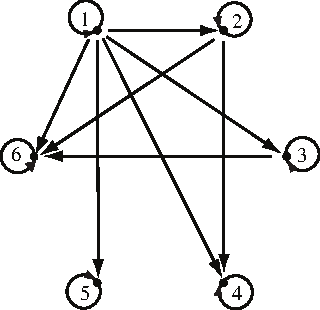
\includegraphics[width=\linewidth]{external/figps-sec71-dirgraph-a.pdf}
\end{sbspanel}%
\begin{sbspanel}{0.4}%
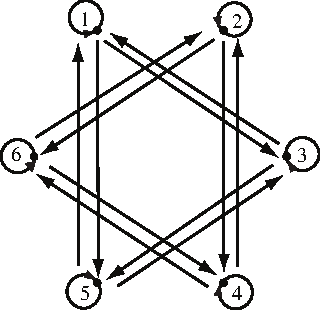
\includegraphics[width=\linewidth]{external/figps-sec71-dirgraph-b.pdf}
\end{sbspanel}%
\end{sidebyside}%
%
\end{inlinesolution}%
\par\medskip
\noindent\textbf{\Large{}7.2\space{}Equivalence Relations\\
\space{}Directed Graphs and Properties of Relations}
\begin{inlinesolution}{7.11}{Properties of Relations.}{x:exercise:prog_proprelations}%
\par\smallskip%
\noindent\hypertarget{g:solution:idm818851224-back}{}The relation \(R\):%
\begin{itemize}[label=\textbullet]
\item{}Is not reflexive since \((c, c) \notin R\) and \((d, d) \notin R\).%
\item{}Is symmetric.%
\item{}Is not transitive. For example, \((c, a) \in R\), \((a, c) \in R\), but \((c, c) \notin R\).%
\end{itemize}
%
\end{inlinesolution}%
\par\medskip
\noindent\textbf{\Large{}\space{}Definition of an Equivalence Relation}
\begin{inlinesolution}{7.13}{A Relation that Is an Equivalence Relation.}{x:exercise:prog_example-equiv}%
\par\smallskip%
\noindent\hypertarget{g:solution:idm818815384-back}{}Proof that the relation \(\sim\) is symmetric: Let \(a,
b \in \Q\) and assume that \(a \sim b\). This means that \(a - b \in \Z\). Therefore, \(-(a - b) \in \Z\) and this means that \(b - a \in \Z\), and hence, \(b \sim a\).%
\par
Proof that the relation \(\sim\) is transitive: Let \(a,
b, c \in \Q\) and assume that \(a \sim b\) and \(b \sim c\). This means that \(a - b \in \Z\) and that \(b - c \in \Z\). Therefore, \(\left((a - b) + (b - c) \right) \in \Z\) and this means that \(a - c \in \Z\), and hence, \(a \sim c\).%
\end{inlinesolution}%
\par\medskip
\noindent\textbf{\Large{}\space{}Examples of Other Equivalence Relations}
\begin{inlinesolution}{7.15}{Another Equivalence Relation.}{x:exercise:prog_anotherequiv}%
\par\smallskip%
\noindent\hypertarget{g:solution:idm818726568-back}{}The relation \(\approx\) is reflexive on \(\mathcal{P}\left( U \right)\) since for all \(A \in \mathcal{P}\left( U \right)\), \(\card(A) = \card(A)\).%
\par
The relation \(\approx\) is symmetric since for all \(A, B \in \mathcal{P}\left( U \right)\), if \(\card(A) = \card(B)\), then using the fact that equality on \(\Z\) is symmetric, we conclude that \(\card(B) = \card(A)\). That is, if \(A\) has the same number of elements as \(B\), then \(B\) has the same number of elements as \(A\).%
\par
The relation \(\approx\) is transitive since for all \(A, B, C \in 
\mathcal{P}\left( U \right)\), if \(\card(A) = \card(B)\) and \(\card(B) = \card(C)\), then using the fact that equality on \(\Z\) is transitive, we conclude that \(\card(A) = \card(C)\). That is, if \(A\) and \(B\) have the same number of elements and \(B\) and \(C\) have the same number of elements, then \(A\) and \(C\) have the same number of elements.%
\par
Therefore, the relation \(\approx\) is an equivalence relation on \(\mathcal{P}\left( U \right)\).%
\end{inlinesolution}%
\par\medskip
\noindent\textbf{\Large{}7.3\space{}Equivalence Classes\\
\space{}The Definition of an Equivalence Class}
\begin{inlinesolution}{7.16}{Equivalence Classes from Beginning Activity 1.}{x:exercise:prog_prev73}%
\par\smallskip%
\noindent\hypertarget{g:solution:idm818453640-back}{}The distinct equivalence classes for the relation \(R\) are: \(\{a, b, e \}\) and \(\{c, d \}\).%
\end{inlinesolution}%
\par\medskip
\noindent\textbf{\Large{}\space{}Congruence Modulo \(\boldsymbol{n}\) and Congruence Classes}
\begin{inlinesolution}{7.17}{Congruence Modulo 4.}{x:exercise:prog_congmod4}%
\par\smallskip%
\noindent\hypertarget{g:solution:idm818436104-back}{}The distinct congruence classes for congruence modulo 4 are%
\begin{align*}
[ 0 ] \amp = \left\{\,\ldots,  -12, -8, -4, 0, 4, 8, 12, \ldots\, \right\}  
\amp [ 1 ] \amp = \left\{\,\ldots,  -11, -7, -3, 1, 5, 9, 13, \ldots\, \right\}\\
[ 2 ] \amp = \left\{\,\ldots,  -10, -6, -2, 2, 6, 10, 14, \ldots\, \right\} 
\amp [ 3 ] \amp = \left\{\,\ldots,  -9, -5, -1, 3, 7, 11, 15, \ldots\, \right\}\text{.}
\end{align*}
%
\end{inlinesolution}%
\par\medskip
\noindent\textbf{\Large{}\space{}Properties of Equivalence Classes}
\begin{inlinesolution}{7.19}{Equivalence Classes.}{x:exercise:prog_equivclass}%
\begin{enumerate}[font=\bfseries,label=(\alph*),ref=\alph*]
\item[(a)]\par\smallskip%
\noindent\hypertarget{g:solution:idm818369160-back}{}\([ 5 ] = [ -5 ] = \left\{ -5, 5 \right\}\)%
\par
\([ 10 ] = [ -10 ] = \left\{ -10, 10 \right\}\)%
\par
\([ \pi ] = [ -\pi ] = 
\left\{ -\pi, \pi \right\}\)%
\item[(b)]\par\smallskip%
\noindent\hypertarget{g:solution:idm818366344-back}{}\([ 0 ] = \left\{ 0 \right\}\)%
\item[(c)]\par\smallskip%
\noindent\hypertarget{g:solution:idm818367112-back}{}\([ a ] = \left\{ -a, a \right\}\)%
\end{enumerate}
\end{inlinesolution}%
\par\medskip
\noindent\textbf{\Large{}7.4\space{}Modular Arithmetic\\
\space{}The Integers Modulo \(\boldsymbol{n}\)}
\begin{inlinesolution}{7.25}{Modular Arithmetic in \(\boldsymbol{\Z_2}\), \(\boldsymbol{\Z_5}\), and \(\boldsymbol{\Z_6}\).}{x:exercise:prog_modulararithmetic5-6}%
\begin{enumerate}[font=\bfseries,label=(\alph*),ref=\alph*]
\item[(a)]\par\smallskip%
\noindent\hypertarget{g:solution:idm817826312-back}{}\begin{sidebyside}{2}{0.1}{0.1}{0.2}%
\begin{sbspanel}{0.3}%
\resizebox{\ifdim\width > \linewidth\linewidth\else\width\fi}{!}{%
{\centering%
{\tabularfont%
\begin{tabular}{lll}
\multicolumn{1}{lA}{\(\oplus\)}&\([ 0 ]\)&\([ 1 ]\)\tabularnewline\hrulemedium
\multicolumn{1}{lA}{\([ 0 ]\)}&\([ 0 ]\)&\([ 1 ]\)\tabularnewline[0pt]
\multicolumn{1}{lA}{\([ 1 ]\)}&\([ 1 ]\)&\([ 0 ]\)
\end{tabular}
}%
\par}
}%
\end{sbspanel}%
\begin{sbspanel}{0.3}%
\resizebox{\ifdim\width > \linewidth\linewidth\else\width\fi}{!}{%
{\centering%
{\tabularfont%
\begin{tabular}{lll}
\multicolumn{1}{lB}{\(\odot\)}&\([ 0 ]\)&\([ 1 ]\)\tabularnewline\hrulemedium
\multicolumn{1}{lB}{\([ 0 ]\)}&\([ 0 ]\)&\([ 0 ]\)\tabularnewline[0pt]
\multicolumn{1}{lB}{\([ 1 ]\)}&\([ 0 ]\)&\([ 1 ]\)
\end{tabular}
}%
\par}
}%
\end{sbspanel}%
\end{sidebyside}%
%
\item[(c)]\par\smallskip%
\noindent\hypertarget{g:solution:idm817780488-back}{}\begin{sidebyside}{2}{0}{0}{0}%
\begin{sbspanel}{0.5}%
\resizebox{\ifdim\width > \linewidth\linewidth\else\width\fi}{!}{%
{\centering%
{\tabularfont%
\begin{tabular}{ccccccc}
\multicolumn{1}{cB}{\(\oplus\)}&\([ 0 ]\)&\([ 1 ]\)&\([ 2 ]\)&\([ 3 ]\)&\([ 4 ]\)&\([ 5 ]\)\tabularnewline\hrulemedium
\multicolumn{1}{cB}{\([ 0 ]\)}&\([ 0 ]\)&\([ 1 ]\)&\([ 2 ]\)&\([ 3 ]\)&\([ 4 ]\)&\([ 5 ]\)\tabularnewline[0pt]
\multicolumn{1}{cB}{\([ 1 ]\)}&\([ 1 ]\)&\([ 2 ]\)&\([ 3 ]\)&\([ 4 ]\)&\([ 5 ]\)&\([ 0 ]\)\tabularnewline[0pt]
\multicolumn{1}{cB}{\([ 2 ]\)}&\([ 2 ]\)&\([ 3 ]\)&\([ 4 ]\)&\([ 5 ]\)&\([ 0 ]\)&\([ 1 ]\)\tabularnewline[0pt]
\multicolumn{1}{cB}{\([ 3 ]\)}&\([ 3 ]\)&\([ 4 ]\)&\([ 5 ]\)&\([ 0 ]\)&\([ 1 ]\)&\([ 2 ]\)\tabularnewline[0pt]
\multicolumn{1}{cB}{\([ 4 ]\)}&\([ 4 ]\)&\([ 5 ]\)&\([ 0 ]\)&\([ 1 ]\)&\([ 2 ]\)&\([ 3 ]\)\tabularnewline[0pt]
\multicolumn{1}{cB}{\([ 5 ]\)}&\([ 5 ]\)&\([ 0 ]\)&\([ 1 ]\)&\([ 2 ]\)&\([ 3 ]\)&\([ 4 ]\)
\end{tabular}
}%
\par}
}%
\end{sbspanel}%
\begin{sbspanel}{0.5}%
\resizebox{\ifdim\width > \linewidth\linewidth\else\width\fi}{!}{%
{\centering%
{\tabularfont%
\begin{tabular}{ccccccc}
\multicolumn{1}{cB}{\(\odot\)}&\([ 0 ]\)&\([ 1 ]\)&\([ 2 ]\)&\([ 3 ]\)&\([ 4 ]\)&\([ 5 ]\)\tabularnewline\hrulemedium
\multicolumn{1}{cB}{\([ 0 ]\)}&\([ 0 ]\)&\([ 0 ]\)&\([ 0 ]\)&\([ 0 ]\)&\([ 0 ]\)&\([ 0 ]\)\tabularnewline[0pt]
\multicolumn{1}{cB}{\([ 1 ]\)}&\([ 0 ]\)&\([ 1 ]\)&\([ 2 ]\)&\([ 3 ]\)&\([ 4 ]\)&\([ 5 ]\)\tabularnewline[0pt]
\multicolumn{1}{cB}{\([ 2 ]\)}&\([ 0 ]\)&\([ 2 ]\)&\([ 4 ]\)&\([ 0 ]\)&\([ 2 ]\)&\([ 4 ]\)\tabularnewline[0pt]
\multicolumn{1}{cB}{\([ 3 ]\)}&\([ 0 ]\)&\([ 3 ]\)&\([ 0 ]\)&\([ 3 ]\)&\([ 0 ]\)&\([ 3 ]\)\tabularnewline[0pt]
\multicolumn{1}{cB}{\([ 4 ]\)}&\([ 0 ]\)&\([ 4 ]\)&\([ 2 ]\)&\([ 0 ]\)&\([ 4 ]\)&\([ 2 ]\)\tabularnewline[0pt]
\multicolumn{1}{cB}{\([ 5 ]\)}&\([ 0 ]\)&\([ 5 ]\)&\([ 4 ]\)&\([ 3 ]\)&\([ 2 ]\)&\([ 1 ]\)
\end{tabular}
}%
\par}
}%
\end{sbspanel}%
\end{sidebyside}%
%
\item[(d)]\par\smallskip%
\noindent\hypertarget{g:solution:idm817536408-back}{}For all \(a, b \in \Z\), if \(a \ne 0\) and \(b \ne 0\), then \(ab \ne 0\).%
\item[(e)]\begin{enumerate}[font=\bfseries,label=(\roman*),ref=\theenumi.\roman*]
\item[(i)]\par\smallskip%
\noindent\hypertarget{g:solution:idm817535000-back}{}The statement in (i) is true.%
\item[(ii)]\par\smallskip%
\noindent\hypertarget{g:solution:idm817531160-back}{}The statement in (ii) is false. For example, in \(\Z_6\), \([ 2 ] \odot [ 3 ] = [ 0 ]\).%
\end{enumerate}
\end{enumerate}
\end{inlinesolution}%
\par\medskip
\noindent\textbf{\Large{}8\space{}Topics in Number Theory\\
8.1\space{}The Greatest Common Divisor\\
\space{}The Greatest Common Divisor}
\begin{inlinesolution}{8.4}{Illustrations of Lemma~{\xreffont\ref*{x:lemma:L_gcdanddivalgo}}.}{x:exercise:prog_lemma81}%
\begin{enumerate}[font=\bfseries,label=(\alph*),ref=\alph*]
\item[(a)]\par\smallskip%
\noindent\hypertarget{g:solution:idm817116952-back}{}The remainder is 8.%
\item[(b)]\par\smallskip%
\noindent\hypertarget{g:solution:idm817116568-back}{}\(\gcd(12, 8) = 4\)%
\item[(c)]\par\smallskip%
\noindent\hypertarget{g:solution:idm817113368-back}{}\(12 = 8 \cdot 1 + 4\) and \(\gcd(r, r_2) = \gcd(8, 4) = 4\)%
\end{enumerate}
\end{inlinesolution}%
\par\medskip
\noindent\textbf{\Large{}\space{}The Euclidean Algorithm}
\begin{inlinesolution}{8.6}{}{x:exercise:prog_usingeuclid}%
\begin{enumerate}[font=\bfseries,label=(\alph*),ref=\alph*]
\item[(a)]\par\smallskip%
\noindent\hypertarget{g:solution:idm817038872-back}{}\begin{center}%
{\tabularfont%
\begin{tabular}{lll}
\multicolumn{1}{lB}{\textbf{Original Pair}}&\multicolumn{1}{lB}{\tablecelllines{l}{m}
{Equation from\\
Division Algorithm}
}&\textbf{New Pair}\tabularnewline\hrulemedium
\multicolumn{1}{lB}{\(\left( {180, 126} \right)\)}&\multicolumn{1}{lB}{\(180 = 126 \cdot 1 + 54\)}&\(\left( {126, 54} \right)\)\tabularnewline\hrulemedium
\multicolumn{1}{lB}{\(\left( {126, 54} \right)\)}&\multicolumn{1}{lB}{\(126 = 54 \cdot 2 + 18\)}&\(\left( {54, 18} \right)\)\tabularnewline\hrulemedium
\multicolumn{1}{lB}{\(\left( {54, 18} \right)\)}&\multicolumn{1}{lB}{\(54 = 18 \cdot 3 + 0\)}&
\end{tabular}
}%
\end{center}%
%
\par
Consequently, \(\gcd( {180, 126} ) = 18\).%
\item[(b)]\par\smallskip%
\noindent\hypertarget{g:solution:idm817028376-back}{}\begin{center}%
{\tabularfont%
\begin{tabular}{lll}
\multicolumn{1}{lB}{\textbf{Original Pair}}&\multicolumn{1}{lB}{\tablecelllines{l}{m}
{Equation from\\
Division Algorithm}
}&\textbf{New Pair}\tabularnewline\hrulemedium
\multicolumn{1}{lB}{\(\left( {4208, 288} \right)\)}&\multicolumn{1}{lB}{\(4208 = 288 \cdot 14 + 176\)}&\(\left( {288, 176} \right)\)\tabularnewline\hrulemedium
\multicolumn{1}{lB}{\(\left( {288, 176} \right)\)}&\multicolumn{1}{lB}{\(288 = 176 \cdot 1 + 112\)}&\(\left( {112, 64} \right)\)\tabularnewline\hrulemedium
\multicolumn{1}{lB}{\(\left( {112, 64} \right)\)}&\multicolumn{1}{lB}{\(112 = 64 \cdot 1 + 48\)}&\(\left( {64, 48} \right)\)\tabularnewline\hrulemedium
\multicolumn{1}{lB}{\(\left( {64, 48} \right)\)}&\multicolumn{1}{lB}{\(64 = 48 \cdot 1 + 16\)}&\(\left( {48, 16} \right)\)\tabularnewline\hrulemedium
\multicolumn{1}{lB}{\(\left( {48, 16} \right)\)}&\multicolumn{1}{lB}{\(48 = 16 \cdot 3 + 0\)}&
\end{tabular}
}%
\end{center}%
%
\par
Consequently, \(\gcd( {4208, 288} ) = 16\)%
\end{enumerate}
\end{inlinesolution}%
\par\medskip
\noindent\textbf{\Large{}\space{}Writing \(\boldsymbol{\gcd (a, b)}\)  in Terms of \(a\) and \(b\)}
\begin{inlinesolution}{8.9}{Writing the gcd as a Linear Combination.}{x:exercise:prog_gcdaslincomb}%
\begin{enumerate}[font=\bfseries,label=(\alph*),ref=\alph*]
\item[(a)]\par\smallskip%
\noindent\hypertarget{g:solution:idm816958632-back}{}From \hyperref[x:exercise:prog_usingeuclid]{Progress Check~{\xreffont\ref{x:exercise:prog_usingeuclid}}, p.\,\pageref{x:exercise:prog_usingeuclid}}, \(\gcd ( {180, 126} ) = 18\).%
\begin{align*}
18 \amp = 126 - 54 \cdot 2\\
\amp = 126 - ( {180 - 126} ) \cdot 2\\
\amp = 126 \cdot 3 + 180 \cdot ( { - 2} )\text{.}
\end{align*}
So \(\gcd ( {180, 126} ) = 18\), and \(18 = 126 \cdot 3 + 180 \cdot ( { - 2} )\).%
\item[(b)]\par\smallskip%
\noindent\hypertarget{g:solution:idm816962472-back}{}From \hyperref[x:exercise:prog_usingeuclid]{Progress Check~{\xreffont\ref{x:exercise:prog_usingeuclid}}, p.\,\pageref{x:exercise:prog_usingeuclid}}, \(\gcd ( {4208, 288} ) = 16\).%
\begin{align*}
16 \amp = 64 - 48\\
\amp = 64 - ( {112 - 64} ) = 64 \cdot 2 - 112\\
\amp = ( {176 - 112} ) \cdot 2 - 112 = 176 \cdot 2 - 112 \cdot 3\\
\amp = 176 \cdot 2 - ( {288 - 176} ) \cdot 3 = 176 \cdot 5 - 288 \cdot 3\\
\amp = ( {4208 - 288 \cdot 14} ) \cdot 5 - 288 \cdot 3\\
\amp = 4208 \cdot 5 + 288 \cdot ( { - 73} )\text{.}
\end{align*}
So \(\gcd ( {4208, 288} ) = 16\), and \(16 = 4208 \cdot 5 + 288 \cdot ( { - 73} )\).%
\end{enumerate}
\end{inlinesolution}%
\par\medskip
\noindent\textbf{\Large{}8.2\space{}Prime Numbers and Prime Factorizations\\
\space{}Relatively Prime Integers}
\begin{inlinesolution}{8.12}{Relatively Prime Integers.}{x:exercise:prog_relativelyprime}%
\begin{enumerate}[font=\bfseries,label=(\alph*),ref=\alph*]
\item[(a)]\par\smallskip%
\noindent\hypertarget{g:solution:idm816776744-back}{}If \(a, p \in \mathbb{Z}\), \(p\) is prime, and \(p\) divides \(a\), then \(\gcd ( {a, p} ) = p\).%
\item[(b)]\par\smallskip%
\noindent\hypertarget{g:solution:idm816764712-back}{}If \(a, p \in \mathbb{Z}\), \(p\) is prime, and \(p\) does not divide \(a\), then \(\gcd ( {a, p} ) = 1\).%
\item[(c)]\par\smallskip%
\noindent\hypertarget{g:solution:idm816755240-back}{}Three examples are \(\gcd ( {4, 9} ) = 1\), \(\gcd ( {15, 16} ) = 1\), \(\gcd ( {8, 25} ) = 1\).%
\end{enumerate}
\end{inlinesolution}%
\begin{inlinesolution}{8.15}{Completing the Proof of Theorem~{\xreffont\ref*{x:theorem:T_relativelyprimeprop}}.}{x:exercise:prog_relativelyprimeprop}%
\par\smallskip%
\noindent\hypertarget{g:solution:idm816719656-back}{}\begin{solutionproof}
Let \(a\), \(b\), and \(c\) be integers. Assume that \(a\) and \(b\) are relatively prime and \(a \mid ( {bc} )\). We will prove that \(a\) divides \(c\).%
\par
Since \(a\) divides \(bc\), there exists an integer \(k\) such that%
\begin{equation}
bc = ak\text{.}\label{x:men:eq_814a}
\end{equation}
%
\par
In addition, we are assuming that \(a\) and \(b\) are relatively prime and hence \(\gcd ( {a, b} ) = 1\). So by \hyperref[x:theorem:T_gcddivideslincombs]{Theorem~{\xreffont\ref{x:theorem:T_gcddivideslincombs}}, p.\,\pageref{x:theorem:T_gcddivideslincombs}}, there exist integers \(m\) and \(n\) such that%
\begin{equation}
am + bn = 1\text{.}\label{x:men:eq_814b}
\end{equation}
%
\par
We now multiply both sides of equation \hyperref[x:men:eq_814b]{({\xreffont\ref{x:men:eq_814b}})} by \(c\). This gives%
\begin{align}
( {am + bn} )c \amp = 1 \cdot c\notag\\
acm + bcn \amp = c\label{x:mrow:eq_814c}
\end{align}
%
\par
We can now use equation 1 to substitute \(bc = ak\) in equation \hyperref[x:mrow:eq_814c]{({\xreffont\ref{x:mrow:eq_814c}})} and obtain%
\begin{equation*}
acm + akn = c\text{.}
\end{equation*}
%
\par
If we now factor the left side of this last equation, we see that \(a( {cm + kn} ) = c\). Since \(( {cm + kn} )\) is an integer, this proves that \(a\) divides \(c\). Hence, we have proven that if \(a\) and \(b\) are relatively prime and \(a \mid ( {bc} )\), then \(a \mid c\).%
\end{solutionproof}
\end{inlinesolution}%
\par\medskip
\noindent\textbf{\Large{}8.3\space{}Linear Diophantine Equations}
\begin{inlinesolution}{8.22}{An Example of a Linear Diophantine Equation.}{x:exercise:prog_lineardioph}%
\begin{enumerate}[font=\bfseries,label=(\alph*),ref=\alph*]
\item[(b)]\par\smallskip%
\noindent\hypertarget{g:solution:idm816327080-back}{}\(x = 2 + 3k\) and \(y = 0 - 2k\), where \(k\) can be any integer. Again, this does not prove that these are the only solutions.%
\end{enumerate}
\end{inlinesolution}%
\begin{inlinesolution}{8.23}{Revisiting Beginning Activity 2.}{x:exercise:prog_prevact2}%
\par\smallskip%
\noindent\hypertarget{g:solution:idm816330152-back}{}One of the Diophantine equations in \hyperlink{x:worksheet:exploringlinear}{Beginning Activity 2, p.\,\pageref{x:worksheet:exploringlinear}} was \(3x + 5y = 11\). We were able to write the solutions of this Diophantine equation in the form%
\begin{equation*}
x = 2 + 5k  \text{ and }   y = 1 - 3k\text{,}
\end{equation*}
where \(k\) is an integer. Notice that \(x = 2\) and \(y = 1\) is a solution of this equation. If we consider this equation to be in the form \(ax + by = c\), then we see that \(a = 3\), \(b = 5\), and \(c = 11\). Solutions for this equation can be written in the form%
\begin{equation*}
x = 2 + bk  \text{ and }   y = 1 - ak\text{,}
\end{equation*}
where \(k\) is an integer.%
\par
The other equation was \(4x + 6y = 16\). So in this case, \(a = 4\), \(b = 6\), and \(c = 16\). Also notice that \(d = \gcd ( 4, 6 ) = 2\). We note that \(x = 4\) and \(y = 0\) is one solution of this Diophantine equation and solutions can be written in the form%
\begin{equation*}
x = 4 + 3k  \text{ and }   y = 0 - 2k\text{,}
\end{equation*}
where \(k\) is an integer. Using the values of \(a\), \(b\), and \(d\) given above, we see that the solutions can be written in the form%
\begin{equation*}
x = 2 + \frac{b}{d} k  \text{ and }   y = 0 - \frac{a}{d}\text{,}
\end{equation*}
where \(k\) is an integer.%
\end{inlinesolution}%
\begin{inlinesolution}{8.26}{Linear Diophantine Equations.}{x:exercise:prog_lindiophequations}%
\begin{enumerate}[font=\bfseries,label=(\alph*),ref=\alph*]
\item[(a)]\par\smallskip%
\noindent\hypertarget{g:solution:idm816276776-back}{}Since 21 does not divide 40, \hyperref[x:theorem:T_lindioph2]{Theorem~{\xreffont\ref{x:theorem:T_lindioph2}}, p.\,\pageref{x:theorem:T_lindioph2}} tells us that the Diophantine equation \(63x + 336y = 40\) has no solutions. Remember that this means there is no ordered pair of integers \(( x, y )\) such that \(63x + 336y = 40\). However, if we allow \(x\) and \(y\) to be real numbers, then there are real number solutions. In fact, we can graph the straight line whose equation is \(63x + 336y = 40\) in the Cartesian plane. From the fact that there is no pair of integers \(x,
y\) such that \(63x + 336y = 40\), we can conclude that there is no point on the graph of this line in which both coordinates are integers.%
\item[(b)]\par\smallskip%
\noindent\hypertarget{g:solution:idm816265256-back}{}To write formulas that will generate all the solutions, we first need to find one solution for \(144x + 225y = 27\). This can sometimes be done by trial and error, but there is a systematic way to find a solution. The first step is to use the Euclidean Algorithm in reverse to write \(\gcd ( {144, 225} )\) as a linear combination of 144 and 225. See \hyperref[x:section:S_gcd]{Section~{\xreffont\ref{x:section:S_gcd}}, p.\,\pageref{x:section:S_gcd}} to review how to do this. The result from using the Euclidean Algorithm in reverse for this situation is%
\begin{equation*}
144 \cdot 11 + 225 \cdot ( {-7} ) = 9\text{.}
\end{equation*}
If we multiply both sides of this equation by 3, we obtain%
\begin{equation*}
144 \cdot 33 + 225 \cdot ( {-21} ) = 27\text{.}
\end{equation*}
This means that \(x_0 = 33,
y_0 = -21\) is a solution of the linear Diophantine equation \(144x + 225y = 27\). We can now use \hyperref[x:theorem:T_lindioph2]{Theorem~{\xreffont\ref{x:theorem:T_lindioph2}}, p.\,\pageref{x:theorem:T_lindioph2}} to conclude that all solutions of this Diophantine equation can be written in the form%
\begin{equation*}
x = 33 + \frac{225}{9} k \qquad y = -21 -\frac{144}{9} k\text{,}
\end{equation*}
where \(k \in \mathbb{Z}\). Simplifying, we see that all solutions can be written in the form%
\begin{equation*}
x = 33 + 25 k \qquad y = -21 -16 k\text{,}
\end{equation*}
where \(k \in \mathbb{Z}\).%
\par
We can check this general solution as follows:  Let \(k \in \mathbb{Z}\). Then%
\begin{align*}
144x + 225y \amp = 144 ( {33 + 25k} ) + 225 ( {-21 - 16k} )\\
\amp = ( {4752 + 3600k} ) + ( {-4725 - 3600k} )\\
\amp = 27\text{.}
\end{align*}
%
\end{enumerate}
\end{inlinesolution}%
\par\medskip
\noindent\textbf{\Large{}9\space{}Finite and Infinite Sets\\
9.1\space{}Finite Sets\\
\space{}Equivalent Sets}
\begin{inlinesolution}{9.2}{Examples of Equivalent Sets.}{x:exercise:prog_equivsets}%
\begin{enumerate}[font=\bfseries,label=(\alph*),ref=\alph*]
\item[(a)]\par\smallskip%
\noindent\hypertarget{g:solution:idm816091176-back}{}We first prove that \(f\x A \to B\) is an injection. So let \(x, y \in A\) and assume that \(f(x) = f(y)\). Then \(x + 350 = y + 350\) and we can conclude that \(x = y\). Hence, \(f\) is an injection. To prove that \(f\) is a surjection, let \(b \in B\). Then \(351 \leq b \leq 450\) and hence, \(1 \leq b - 350 \leq 100\) and so \(b - 350 \in A\). In addition, \(f(b - 350) = (b - 350) + 350 = b\). This proves that \(f\) is a surjection. Hence, the function \(f\) is a bijection, and so, \(A \approx B\).%
\item[(b)]\par\smallskip%
\noindent\hypertarget{g:solution:idm816071704-back}{}If \(x\) and \(t\) are even integers and \(F ( x ) = F ( t )\), then \(x + 1 = t + 1\) and, hence, \(x = t\). Therefore, \(F\) is an injection. To prove that \(F\) is a surjection, let \(y \in D\). This means that \(y\) is an odd integer and, hence, \(y - 1\) is an even integer. In addition,%
\begin{equation*}
F ( y - 1 ) = ( y - 1 ) + 1 = y\text{.}
\end{equation*}
Therefore, \(F\) is a surjection and hence, \(F\) is a bijection. We conclude that \(E \approx D\).%
\item[(c)]\par\smallskip%
\noindent\hypertarget{g:solution:idm816062488-back}{}Let \(x, t \in ( 0, 1 )\) and assume that \(f ( x ) = f ( t )\). Then \(bx = bt\) and, hence, \(x = t\). Therefore, \(f\) is an injection. To prove that \(f\) is a surjection, let \(y \in ( 0, b )\). Since \(0 \lt  y \lt  b\), we conclude that \(0 \lt  \dfrac{y}{b} \lt  1\) and that%
\begin{equation*}
f \!\left( \dfrac{y}{b} \right) = b \!\left( \dfrac{y}{b} \right) = y\text{.}
\end{equation*}
Therefore, \(f\) is a surjection and hence \(f\) is a bijection. Thus, \(( 0, 1 ) \approx ( 0, b )\).%
\end{enumerate}
\end{inlinesolution}%
\par\medskip
\noindent\textbf{\Large{}9.2\space{}Countable Sets\\
\space{}Infinite Sets}
\begin{inlinesolution}{9.12}{Examples of Infinite Sets.}{x:exercise:E_infinitesets}%
\begin{enumerate}[font=\bfseries,label=(\alph*),ref=\alph*]
\item[(a)]\par\smallskip%
\noindent\hypertarget{g:solution:idm815721112-back}{}The set of natural numbers \(\N\) is a subset of \(\Z\), \(\Q\), and \(\R\). Since \(\N\) is an infinite set, we can use \hyperlink{x:li:T_subsetisinfinite2}{Item~{\xreffont 2}, p.\,\pageref{x:li:T_subsetisinfinite2}} of \hyperref[x:theorem:T_subsetisinfinite]{Theorem~{\xreffont\ref{x:theorem:T_subsetisinfinite}}, p.\,\pageref{x:theorem:T_subsetisinfinite}} to conclude that \(\Z\), \(\Q\), and \(\R\) are infinite sets.%
\item[(b)]\par\smallskip%
\noindent\hypertarget{g:solution:idm815712920-back}{}Use \hyperlink{x:li:T_subsetisinfinite1}{Item~{\xreffont 1}, p.\,\pageref{x:li:T_subsetisinfinite1}} of \hyperref[x:theorem:T_subsetisinfinite]{Theorem~{\xreffont\ref{x:theorem:T_subsetisinfinite}}, p.\,\pageref{x:theorem:T_subsetisinfinite}}.%
\item[(c)]\par\smallskip%
\noindent\hypertarget{g:solution:idm815715864-back}{}Prove that \(E^+ \approx \N\) and use \hyperlink{x:li:T_subsetisinfinite1}{Item~{\xreffont 1}, p.\,\pageref{x:li:T_subsetisinfinite1}} of \hyperref[x:theorem:T_subsetisinfinite]{Theorem~{\xreffont\ref{x:theorem:T_subsetisinfinite}}, p.\,\pageref{x:theorem:T_subsetisinfinite}}.%
\end{enumerate}
\end{inlinesolution}%
\par\medskip
\noindent\textbf{\Large{}\space{}Countably Infinite Sets}
\begin{inlinesolution}{9.13}{Examples of Countably Infinite Sets.}{x:exercise:prog_countablyinfinitesets}%
\begin{enumerate}[font=\bfseries,label=(\alph*),ref=\alph*]
\item[(a)]\par\smallskip%
\noindent\hypertarget{g:solution:idm815689624-back}{}Use the definition of a countably infinite set.%
\item[(b)]\par\smallskip%
\noindent\hypertarget{g:solution:idm815687576-back}{}Since \(E^+ \approx \N\), we can conclude that \(\text{ card} ( E^+ ) = \aleph_0\).%
\item[(c)]\par\smallskip%
\noindent\hypertarget{g:solution:idm815686040-back}{}One function that can be used is \(f\x S \to \N\) defined by \(f(m) = \sqrt{m}\) for all \(m \in S\).%
\end{enumerate}
\end{inlinesolution}%
\par\medskip
\noindent\textbf{\Large{}9.3\space{}Uncountable Sets\\
\space{}Uncountable Subsets of \(\boldsymbol{\mathbb{R}}\)}
\begin{inlinesolution}{9.28}{Dodge Ball and Cantor's Diagonal Argument.}{x:exercise:prog_diagonal}%
\par\smallskip%
\noindent\hypertarget{g:solution:idm815201560-back}{}Player Two has a winning strategy. On the \(k\)th turn, whatever symbol Player One puts in the \(k\)th position of the \(k\)th row, Player Two must put the other symbol in the \(k\)th position of his or her row. This guarantees that the row of symbols produced by Player Two will be different than any of the rows produced by Player One.%
\par
This is the same idea used in Cantor's Diagonal Argument. Once we have a ``list'' of real numbers in normalized form, we create a real number that is not in the list by making sure that its \(k\)th decimal place is different than the \(k\)th decimal place for the \(k\)th number in the list. The one complication is that we must make sure that our new real number does not have a decimal expression that ends in all 9's. This was done by using only 3's and 5's.%
\end{inlinesolution}%
\begin{inlinesolution}{9.30}{Proof of Theorem~{\xreffont\ref*{x:theorem:T_openintervals}}.}{x:exercise:prog_openintervals}%
\begin{enumerate}[font=\bfseries,label=(\alph*),ref=\alph*]
\item[(a)]\par\smallskip%
\noindent\hypertarget{g:solution:idm815172504-back}{}\begin{solutionproof}
In order to find a bijection \(f\x  ( 0, 1 ) \to ( a, b )\), we will use the linear function through the points \(( 0, a )\) and \(( 1, b )\). The slope is \(( b - a)\) and the \(y\)-intercept is \(( 0, a )\). So define \(f\x  ( 0, 1 ) \to ( a, b )\) by \(f ( x ) = ( b - a )x + a\), for each \(x \in ( 0, 1 )\). Now, if \(x,
t \in ( 0, 1 )\) and \(f ( x ) = f ( t )\), then%
\begin{equation*}
( b - a )x + a = ( b - a )t + a\text{.}
\end{equation*}
%
\par
This implies that \(( b - a )x = ( b - a )t\), and since \(b - a \ne 0\), we can conclude that \(x = t\). Therefore, \(f\) is an injection.%
\par
To prove that \(f\) is a surjection, we let \(y \in ( a, b )\). If \(x = \dfrac{y - a}{b - a}\), then%
\begin{align*}
f ( x ) \amp = f \!\left( \frac{y - a}{b - a} \right)\\
\amp = ( b - a ) \!\left( \frac{y - a}{b - a} \right) + a\\
\amp = ( y - a ) + a\\
\amp = y\text{.}
\end{align*}
%
\par
This proves that \(f\) is a surjection. Hence, \(f\) is a bijection and \(( 0, 1 ) \approx ( a, b )\). Therefore, \(( a, b )\) is uncountable and has cardinality \(\boldsymbol{c}\).%
\end{solutionproof}
\item[(b)]\par\smallskip%
\noindent\hypertarget{g:solution:idm815155480-back}{}Now, if \(a,
b, c, d\) are real numbers with \(a \lt b\) and \(c \lt d\), then we know that \(( a, b ) \approx ( 0, 1 )\) and \(( c, d ) \approx ( 0, 1 )\). Since \(\approx\) is an equivalence relation,we can conclude that \(( a, b ) \approx ( c, d )\).%
\end{enumerate}
\end{inlinesolution}%
\end{solutions-chapter}
%
%
\typeout{************************************************}
\typeout{Appendix C Answers and Hints for Selected Exercises}
\typeout{************************************************}
%
\begin{solutions-chapter}{Answers and Hints for Selected Exercises}{}{Answers and Hints for Selected Exercises}{}{}{x:solutions:exer-answers}
\par\medskip
\noindent\textbf{\Large{}1\space{}Introduction to Writing Proofs in Mathematics\\
1.1\space{}Statements and Conditional Statements\\
\space{}Exercises}
\begin{divisionsolution}{1}{}{x:exercise:exer_sec11-1}%
\begin{enumerate}[font=\bfseries,label=(\alph*),ref=\alph*]
\item[(a)]\par\smallskip%
\hypertarget{g:answer:idm830792216-back}{}\quad{}This is a statement.%
\item[(b)]\par\smallskip%
\hypertarget{g:answer:idm830793240-back}{}\quad{}This is not a statement.%
\item[(c)]\par\smallskip%
\hypertarget{g:answer:idm830792088-back}{}\quad{}This is a statement.%
\item[(d)]\par\smallskip%
\hypertarget{g:answer:idm830781336-back}{}\quad{}This is not a statement.%
\item[(e)]\par\smallskip%
\hypertarget{g:answer:idm830781080-back}{}\quad{}This is a statement.%
\item[(f)]\par\smallskip%
\hypertarget{g:answer:idm830780568-back}{}\quad{}This is a statement.%
\item[(g)]\par\smallskip%
\hypertarget{g:answer:idm830783256-back}{}\quad{}This is not a statement.%
\item[(h)]\par\smallskip%
\hypertarget{g:answer:idm830783768-back}{}\quad{}This is a statement if we are assuming that \(n\) is a prime number means that \(n\) is a natural number.%
\item[(i)]\par\smallskip%
\hypertarget{g:answer:idm830771608-back}{}\quad{}This is not a statement.%
\item[(j)]\par\smallskip%
\hypertarget{g:answer:idm830776216-back}{}\quad{}This is a statement.%
\item[(k)]\par\smallskip%
\hypertarget{g:answer:idm830770456-back}{}\quad{}This is a statement.%
\end{enumerate}
\end{divisionsolution}%
\begin{divisionsolution}{2}{}{g:exercise:idm830769560}%
\begin{enumerate}[font=\bfseries,label=(\alph*),ref=\alph*]
\item[(a)]\par\smallskip%
\hypertarget{g:answer:idm830771992-back}{}\quad{}Hypothesis: \(n\) is a prime number.%
\par
Conclusion: \(n^2\) has three positive divisors.%
\item[(b)]\par\smallskip%
\hypertarget{g:answer:idm830766616-back}{}\quad{}Hypothesis: \(a\) is an irrational number and \(b\) is an irrational number.%
\par
Conclusion: \(a \cdot b\) is an irrational number.%
\item[(c)]\par\smallskip%
\hypertarget{g:answer:idm830767640-back}{}\quad{}Hypothesis: \(p\) is a prime number%
\par
Conclusion: \(p = 2\) or \(p\) is an odd number.%
\item[(d)]\par\smallskip%
\hypertarget{g:answer:idm831029528-back}{}\quad{}Hypothesis: \(p\) is a prime number and \(p \ne 2\).%
\par
Conclusion: \(p\) is an odd number.%
\item[(e)]\par\smallskip%
\hypertarget{g:answer:idm831024280-back}{}\quad{}Hypothesis: \(p \ne 2\) and \(p\) is an even number.%
\par
Conclusion: \(p\) is not prime.%
\end{enumerate}
\end{divisionsolution}%
\begin{divisionsolution}{3}{}{x:exercise:exer_sec11-3}%
\begin{enumerate}[font=\bfseries,label=(\alph*),ref=\alph*]
\item[(a)]\par\smallskip%
\hypertarget{g:answer:idm830756264-back}{}\quad{}This statement is true.%
\item[(b)]\par\smallskip%
\hypertarget{g:answer:idm830760488-back}{}\quad{}This statement is false.%
\item[(c)]\par\smallskip%
\hypertarget{g:answer:idm830755880-back}{}\quad{}This statement is true.%
\item[(d)]\par\smallskip%
\hypertarget{g:answer:idm830757928-back}{}\quad{}This statement is true.%
\end{enumerate}
\end{divisionsolution}%
\begin{divisionsolution}{4}{}{x:exercise:exer_sec11-4}%
\begin{enumerate}[font=\bfseries,label=(\alph*),ref=\alph*]
\item[(a)]\par\smallskip%
\hypertarget{g:answer:idm830745128-back}{}\quad{}True when \(a \ne 3\).%
\item[(b)]\par\smallskip%
\hypertarget{g:answer:idm830751912-back}{}\quad{}True when \(a = 3\).%
\end{enumerate}
\end{divisionsolution}%
\begin{divisionsolution}{6}{}{x:exercise:exer_sec11-6}%
\begin{enumerate}[font=\bfseries,label=(\alph*),ref=\alph*]
\item[(a)]\par\smallskip%
\hypertarget{g:answer:idm830730536-back}{}\quad{}This function has a maximum value when \(x = \dfrac{5}{16}\).%
\item[(b)]\par\smallskip%
\hypertarget{g:answer:idm830733352-back}{}\quad{}This function has a maximum value when \(x = \dfrac{9}{2}\).%
\item[(c)]\par\smallskip%
\hypertarget{g:answer:idm830735016-back}{}\quad{}No conclusion can be made about this function from this theorem.%
\end{enumerate}
\end{divisionsolution}%
\begin{divisionsolution}{9}{}{x:exercise:exer_sec11_8}%
\begin{enumerate}[font=\bfseries,label=(\alph*),ref=\alph*]
\item[(a)]\par\smallskip%
\hypertarget{g:answer:idm830698920-back}{}\quad{}The set of natural numbers is not closed under division.%
\item[(b)]\par\smallskip%
\hypertarget{g:answer:idm830702504-back}{}\quad{}The set of rational numbers is not closed under division since division by zero is not defined.%
\item[(c)]\par\smallskip%
\hypertarget{g:answer:idm830700584-back}{}\quad{}The set of nonzero rational numbers is closed under division.%
\item[(d)]\par\smallskip%
\hypertarget{g:answer:idm830702888-back}{}\quad{}The set of positive rational numbers is closed under division.%
\item[(e)]\par\smallskip%
\hypertarget{g:answer:idm830697384-back}{}\quad{}The set of positive real numbers is not closed under subtraction.%
\item[(f)]\par\smallskip%
\hypertarget{g:answer:idm830697896-back}{}\quad{}The set of negative rational numbers is not closed under division.%
\item[(g)]\par\smallskip%
\hypertarget{g:answer:idm830702248-back}{}\quad{}The set of negative integers is closed under addition.%
\end{enumerate}
\end{divisionsolution}%
\par\medskip
\noindent\textbf{\Large{}1.2\space{}Constructing Direct Proofs\\
\space{}Exercises}
\begin{divisionsolution}{1}{}{x:exercise:exer_evenodd}%
\begin{enumerate}[font=\bfseries,label=(\alph*),ref=\alph*]
\item[(a)]\par\smallskip%
\hypertarget{g:answer:idm830244888-back}{}\quad{}\begin{center}%
{\tabularfont%
\begin{tabular}{lll}
\multicolumn{1}{lB}{\textbf{Step}}&\multicolumn{1}{lB}{\textbf{Know}}&\textbf{Reason}\tabularnewline\hrulemedium
\multicolumn{1}{lB}{\(P\)}&\multicolumn{1}{lB}{\(m\) is an even integer.}&Hypothesis\tabularnewline\hrulemedium
\multicolumn{1}{lB}{\(P1\)}&\multicolumn{1}{lB}{\tablecelllines{l}{m}
{There exists an integer \(k\)\\
such that \(m = 2k\).}
}&Definition of an even integer\tabularnewline\hrulemedium
\multicolumn{1}{lB}{\(P2\)}&\multicolumn{1}{lB}{\(m + 1 = 2k + 1\)}&Algebra\tabularnewline\hrulemedium
\multicolumn{1}{lB}{\(Q1\)}&\multicolumn{1}{lB}{\tablecelllines{l}{m}
{There exists an integer \(q\)\\
such that \(m +1 = 2q+1\).}
}&Substitution of \(k = q\)\tabularnewline\hrulemedium
\multicolumn{1}{lB}{\(Q\)}&\multicolumn{1}{lB}{\(m + 1\) is an odd integer.}&Definition of an odd integer
\end{tabular}
}%
\end{center}%
%
\end{enumerate}
\end{divisionsolution}%
\begin{divisionsolution}{2}{}{x:exercise:exer_evenoddadd}%
\begin{enumerate}[font=\bfseries,label=(\alph*),ref=\alph*]
\item[(c)]\par\smallskip%
\hypertarget{g:answer:idm830226968-back}{}\quad{}We assume that \(x\) and \(y\) are odd integers and will prove that \(x+y\) is an even integer.  Since \(x\) and \(y\) are odd, there exist integers \(m\) and \(n\) such that \(x = 2m + 1\) and \(y = 2n+1\). Then%
\begin{align*}
x + y \amp = \left( 2m + 1 \right) + \left( 2n + 1 \right)\\
\amp = 2m + 2n + 2\\
\amp = 2 \left( m + n + 1 \right)\text{.}
\end{align*}
Since the integers are closed under addition, \(\left( m + n + 1 \right)\) is an integer, and hence the last equation shows that \(x + y\) is even. Therefore, we have proven that if \(x\) and \(y\) are odd integers, then \(x+y\) is an even integer.%
\end{enumerate}
\end{divisionsolution}%
\begin{divisionsolution}{3}{}{x:exercise:exer_evenoddmult}%
\begin{enumerate}[font=\bfseries,label=(\alph*),ref=\alph*]
\item[(a)]\par\smallskip%
\hypertarget{g:answer:idm830213656-back}{}\quad{}\begin{center}%
{\tabularfont%
\begin{tabular}{lll}
\multicolumn{1}{lB}{\textbf{Step}}&\multicolumn{1}{lB}{\textbf{Know}}&\textbf{Reason}\tabularnewline\hrulemedium
\multicolumn{1}{lB}{\(P\)}&\multicolumn{1}{lB}{\tablecelllines{l}{m}
{\(m\) is an even integer and\\
\(n\) is an integer.}
}&Hypothesis\tabularnewline\hrulemedium
\multicolumn{1}{lB}{\(P1\)}&\multicolumn{1}{lB}{There exists an integer \(k\) \(m = 2k\).}&Definition of an even integer.\tabularnewline\hrulemedium
\multicolumn{1}{lB}{\(P2\)}&\multicolumn{1}{lB}{\(m \cdot n = \left( 2k \right) n\)}&Substitution\tabularnewline\hrulemedium
\multicolumn{1}{lB}{\(P3\)}&\multicolumn{1}{lB}{\(m \cdot n = 2 \left( {kn} \right)\)}&Algebra\tabularnewline\hrulemedium
\multicolumn{1}{lB}{\(P4\)}&\multicolumn{1}{lB}{\(\left( {kn} \right)\) is an integer}&Closure properties of the integers\tabularnewline\hrulemedium
\multicolumn{1}{lB}{\(Q1\)}&\multicolumn{1}{lB}{\tablecelllines{l}{m}
{There exists an integer \(q\)\\
such that \(m \cdot n = 2q\)}
}&\(q = kn\).\tabularnewline\hrulemedium
\multicolumn{1}{lB}{\(Q\)}&\multicolumn{1}{lB}{\(m \cdot n\) is an even integer.}&Definition of an even integer.
\end{tabular}
}%
\end{center}%
%
\item[(b)]\par\smallskip%
\hypertarget{g:answer:idm830199576-back}{}\quad{}Use \hyperref[x:task:exer_evenoddmulta]{Task~{\xreffont 3}.{\xreffont\ref{x:task:exer_evenoddmulta}}, p.\,\pageref{x:task:exer_evenoddmulta}} to answer this.%
\end{enumerate}
\end{divisionsolution}%
\begin{divisionsolution}{4}{}{x:exercise:exer_5m_7}%
\begin{enumerate}[font=\bfseries,label=(\alph*),ref=\alph*]
\item[(a)]\par\smallskip%
\hypertarget{g:answer:idm830200856-back}{}\quad{}We assume that \(m\) is an even integer and will prove that \(5m + 7\) is an odd integer.  Since \(m\) is an even integer, there exists an integer \(k\) such that \(m = 2k\).  Using substitution and algebra, we see that%
\begin{align*}
5m + 7 \amp = 5(2k) + 7\\
\amp = 10k + 6 + 1\\
\amp = 2(5k + 3) + 1
\end{align*}
By the closure properties of the integers, we conclude that \(5k + 3\) is an integer, and so the last equation proves that \(5m + 7\) is an odd integer.%
\par
Another proof. By \hyperref[x:task:exer_evenoddadda]{Task~{\xreffont 2}.{\xreffont\ref{x:task:exer_evenoddadda}}, p.\,\pageref{x:task:exer_evenoddadda}} of \hyperlink{x:exercise:exer_evenoddadd}{Exercise~{\xreffont 2}, p.\,\pageref{x:exercise:exer_evenoddadd}}, \(5m\) is an even integer.  Hence, by \hyperref[x:task:exer_evenoddaddb]{Task~{\xreffont 2}.{\xreffont\ref{x:task:exer_evenoddaddb}}, p.\,\pageref{x:task:exer_evenoddaddb}} of \hyperlink{x:exercise:exer_evenoddadd}{Exercise~{\xreffont 2}, p.\,\pageref{x:exercise:exer_evenoddadd}}, \(5m + 7\) is an even integer.%
\end{enumerate}
\end{divisionsolution}%
\begin{divisionsolution}{5}{}{x:exercise:exer_3m2}%
\begin{enumerate}[font=\bfseries,label=(\alph*),ref=\alph*]
\item[(b)]\par\smallskip%
\hypertarget{g:answer:idm830182296-back}{}\quad{}We assume that \(m\) is an odd integer and will prove that \(3m^2 + 7m + 12\) is an even integer.  Since \(m\) is odd, there exists an integer \(k\) such that \(m = 2k +1\). Hence,%
\begin{align*}
3m^2 + 7m + 12 \amp = 3 \left( 2k + 1 \right)^2 + 7 \left( 2k + 1 \right) + 12\\
\amp = 12k^2 + 26k + 22\\
\amp = 2 \left( 6k^2 + 13k + 11 \right)
\end{align*}
By the closure properties of the integers, \(\left( 6k^2 + 13k + 11 \right)\) is an integer. Hence, this proves that if \(m\) is odd, then \(3m^2 + 7m + 12\) is an even integer.%
\end{enumerate}
\end{divisionsolution}%
\begin{divisionsolution}{6}{}{x:exercise:exer_sec12-7}%
\begin{enumerate}[font=\bfseries,label=(\alph*),ref=\alph*]
\item[(a)]\par\smallskip%
\hypertarget{g:answer:idm830173464-back}{}\quad{}Prove that they are not zero and their quotient is equal to 1.%
\item[(d)]\par\smallskip%
\hypertarget{g:answer:idm830171288-back}{}\quad{}Prove that two of the sides have the same length. Prove that the triangle has two congruent angles.  Prove that an altitude of the triangle is a perpendicular bisector of a side of the triangle.%
\end{enumerate}
\end{divisionsolution}%
\begin{divisionsolution}{9}{}{x:exercise:exer_sec12-type}%
\begin{enumerate}[font=\bfseries,label=(\alph*),ref=\alph*]
\item[(a)]\par\smallskip%
\hypertarget{g:answer:idm830161432-back}{}\quad{}Some examples of type 1 integers are \(-5\), \(-2\), 1, 4, 7, 10.%
\item[(c)]\par\smallskip%
\hypertarget{g:answer:idm830156184-back}{}\quad{}All examples should indicate the proposition is true.%
\end{enumerate}
\end{divisionsolution}%
\begin{divisionsolution}{10}{}{x:exercise:exer_sec12-typeproof}%
\begin{enumerate}[font=\bfseries,label=(\alph*),ref=\alph*]
\item[(a)]\par\smallskip%
\hypertarget{g:answer:idm830152472-back}{}\quad{}Let \(a\) and \(b\) be integers and assume that \(a\) and \(b\) are both type 1 integers.  Then, there exist integers \(m\) and \(n\) such that \(a = 3m + 1\) and \(b = 3n + 1\).  Now show that%
\begin{equation*}
a + b = 3 \left( m + n \right) + 2\text{.}
\end{equation*}
The closure properties of the integers imply that \(m + n\) is an integer. Therefore, the last equation tells us that \(a + b\) is a type 2 integer. Hence, we have proved that if \(a\) and \(b\) are both type 1 integers, then \(a + b\) is a type 2 integer.%
\end{enumerate}
\end{divisionsolution}%
\par\medskip
\noindent\textbf{\Large{}2\space{}Logical Reasoning\\
2.1\space{}Statements and Logical Operators\\
\space{}Exercises}
\begin{divisionsolution}{1}{}{x:exercise:exer_sec22-1}%
\par\smallskip%
\hypertarget{g:answer:idm829730088-back}{}\quad{}The statement was true. When the hypothesis is false, the conditional statement is true.%
\end{divisionsolution}%
\begin{divisionsolution}{2}{}{x:exercise:exer_sec22-2}%
\begin{enumerate}[font=\bfseries,label=(\alph*),ref=\alph*]
\item[(a)]\par\smallskip%
\hypertarget{g:answer:idm829730216-back}{}\quad{}\(P\) is false.%
\item[(b)]\par\smallskip%
\hypertarget{g:answer:idm829729960-back}{}\quad{}\(P \wedge Q\) is false.%
\item[(c)]\par\smallskip%
\hypertarget{g:answer:idm829735848-back}{}\quad{}\(P \vee Q\) is false.%
\end{enumerate}
\end{divisionsolution}%
\begin{divisionsolution}{4}{}{x:exercise:exer_statements4}%
\begin{enumerate}[font=\bfseries,label=(\alph*),ref=\alph*]
\item[(c)]\par\smallskip%
\hypertarget{g:answer:idm829720232-back}{}\quad{}Statement \(P\) is true but since we do not know if \(R\) is true or false, we cannot tell if \(P \wedge R\) is true or false.%
\end{enumerate}
\end{divisionsolution}%
\begin{divisionsolution}{5}{}{x:exercise:exer_sec22-5}%
\begin{enumerate}[font=\bfseries,label=(\alph*),ref=\alph*]
\item[(a)]\par\smallskip%
\hypertarget{g:answer:idm829719080-back}{}\quad{}\begin{center}%
{\tabularfont%
\begin{tabular}{ccc}
\multicolumn{1}{cB}{\(P\)}&\multicolumn{1}{cC}{\(Q\)}&\(P \to Q\)\tabularnewline\hrulethick
\multicolumn{1}{cB}{T}&\multicolumn{1}{cC}{T}&T\tabularnewline[0pt]
\multicolumn{1}{cB}{T}&\multicolumn{1}{cC}{F}&F\tabularnewline[0pt]
\multicolumn{1}{cB}{F}&\multicolumn{1}{cC}{T}&T\tabularnewline[0pt]
\multicolumn{1}{cB}{F}&\multicolumn{1}{cC}{T}&T
\end{tabular}
}%
\end{center}%
%
\item[(b)]\par\smallskip%
\hypertarget{g:answer:idm829706536-back}{}\quad{}\begin{center}%
{\tabularfont%
\begin{tabular}{ccc}
\multicolumn{1}{cB}{\(P\)}&\multicolumn{1}{cC}{\(Q\)}&\(Q \to P\)\tabularnewline\hrulethick
\multicolumn{1}{cB}{T}&\multicolumn{1}{cC}{T}&T\tabularnewline[0pt]
\multicolumn{1}{cB}{T}&\multicolumn{1}{cC}{F}&T\tabularnewline[0pt]
\multicolumn{1}{cB}{F}&\multicolumn{1}{cC}{T}&F\tabularnewline[0pt]
\multicolumn{1}{cB}{F}&\multicolumn{1}{cC}{F}&T
\end{tabular}
}%
\end{center}%
%
\item[(c)]\par\smallskip%
\hypertarget{g:answer:idm829696424-back}{}\quad{}\begin{center}%
{\tabularfont%
\begin{tabular}{ccc}
\multicolumn{1}{cB}{\(P\)}&\multicolumn{1}{cC}{\(Q\)}&\(Q \to P\)\tabularnewline\hrulethick
\multicolumn{1}{cB}{T}&\multicolumn{1}{cC}{T}&T\tabularnewline[0pt]
\multicolumn{1}{cB}{T}&\multicolumn{1}{cC}{F}&T\tabularnewline[0pt]
\multicolumn{1}{cB}{F}&\multicolumn{1}{cC}{T}&F\tabularnewline[0pt]
\multicolumn{1}{cB}{F}&\multicolumn{1}{cC}{F}&T
\end{tabular}
}%
\end{center}%
%
\item[(d)]\par\smallskip%
\hypertarget{g:answer:idm829691048-back}{}\quad{}\begin{center}%
{\tabularfont%
\begin{tabular}{ccc}
\multicolumn{1}{cB}{\(P\)}&\multicolumn{1}{cC}{\(Q\)}&\(P \to Q\)\tabularnewline\hrulethick
\multicolumn{1}{cB}{T}&\multicolumn{1}{cC}{T}&T\tabularnewline[0pt]
\multicolumn{1}{cB}{T}&\multicolumn{1}{cC}{F}&F\tabularnewline[0pt]
\multicolumn{1}{cB}{F}&\multicolumn{1}{cC}{T}&T\tabularnewline[0pt]
\multicolumn{1}{cB}{F}&\multicolumn{1}{cC}{T}&T
\end{tabular}
}%
\end{center}%
%
\item[(e)]\par\smallskip%
\hypertarget{g:answer:idm829686056-back}{}\quad{}Statements (a) and (d) have the same truth table. Statements (b) and (c) have the same truth table.%
\end{enumerate}
\end{divisionsolution}%
\begin{divisionsolution}{7}{}{x:exercise:exer_sec22-6}%
\par\smallskip%
\hypertarget{g:answer:idm829672728-back}{}\quad{}\begin{center}%
{\tabularfont%
\begin{tabular}{ccccc}
\multicolumn{1}{cB}{\(P\)}&\multicolumn{1}{cB}{\(Q\)}&\multicolumn{1}{cC}{\(R\)}&\multicolumn{1}{cB}{\(P \wedge (Q \vee R)\)}&\((P \wedge Q) \vee (P \wedge R)\)\tabularnewline\hrulethick
\multicolumn{1}{cB}{T}&\multicolumn{1}{cB}{T}&\multicolumn{1}{cC}{T}&\multicolumn{1}{cB}{T}&T\tabularnewline[0pt]
\multicolumn{1}{cB}{T}&\multicolumn{1}{cB}{T}&\multicolumn{1}{cC}{F}&\multicolumn{1}{cB}{T}&T\tabularnewline[0pt]
\multicolumn{1}{cB}{T}&\multicolumn{1}{cB}{F}&\multicolumn{1}{cC}{T}&\multicolumn{1}{cB}{T}&T\tabularnewline[0pt]
\multicolumn{1}{cB}{T}&\multicolumn{1}{cB}{F}&\multicolumn{1}{cC}{F}&\multicolumn{1}{cB}{F}&F\tabularnewline[0pt]
\multicolumn{1}{cB}{F}&\multicolumn{1}{cB}{T}&\multicolumn{1}{cC}{T}&\multicolumn{1}{cB}{F}&F\tabularnewline[0pt]
\multicolumn{1}{cB}{F}&\multicolumn{1}{cB}{T}&\multicolumn{1}{cC}{F}&\multicolumn{1}{cB}{F}&F\tabularnewline[0pt]
\multicolumn{1}{cB}{F}&\multicolumn{1}{cB}{F}&\multicolumn{1}{cC}{T}&\multicolumn{1}{cB}{F}&F\tabularnewline[0pt]
\multicolumn{1}{cB}{F}&\multicolumn{1}{cB}{F}&\multicolumn{1}{cC}{F}&\multicolumn{1}{cB}{F}&F
\end{tabular}
}%
\end{center}%
%
\par
The two statements have the same truth table.%
\end{divisionsolution}%
\begin{divisionsolution}{9}{}{x:exercise:exer_sec22-8}%
\begin{enumerate}[font=\bfseries,label=(\alph*),ref=\alph*]
\item[(c)]\par\smallskip%
\hypertarget{g:answer:idm829641240-back}{}\quad{}The integer \(x\) is even only if \(x^2\)  is even.%
\item[(d)]\par\smallskip%
\hypertarget{g:answer:idm829639704-back}{}\quad{}For the integer \(x\) to be even, it is necessary that \(x^2\) be even.%
\end{enumerate}
\end{divisionsolution}%
\begin{divisionsolution}{11}{}{x:exercise:exer_tautology-contra}%
\begin{enumerate}[font=\bfseries,label=(\alph*),ref=\alph*]
\item[(a)]\par\smallskip%
\hypertarget{g:answer:idm829631512-back}{}\quad{}\(\mynot Q \vee (P \to Q)\) is a tautology.%
\item[(b)]\par\smallskip%
\hypertarget{g:answer:idm829635736-back}{}\quad{}\(Q \wedge (P \wedge \mynot Q)\) is a contradiction.%
\item[(c)]\par\smallskip%
\hypertarget{g:answer:idm829634840-back}{}\quad{}\((Q \wedge P) \wedge (P \to \mynot Q)\) is a contradiction.%
\item[(d)]\par\smallskip%
\hypertarget{g:answer:idm829636504-back}{}\quad{}\(\mynot Q \to (P \wedge \mynot P)\) is neither a tautology nor a contradiction.%
\end{enumerate}
\end{divisionsolution}%
\par\medskip
\noindent\textbf{\Large{}2.2\space{}Logically Equivalent Statements\\
\space{}Exercises}
\begin{divisionsolution}{1}{}{x:exercise:exer_sec23-1}%
\begin{enumerate}[font=\bfseries,label=(\alph*),ref=\alph*]
\item[(a)]\par\smallskip%
\hypertarget{g:answer:idm829466008-back}{}\quad{}Converse: If \(a^2 = 25\), then \(a = 5\). Contrapositive: If \(a^2 \ne 25\), then \(a \ne 5\).%
\item[(b)]\par\smallskip%
\hypertarget{g:answer:idm829458584-back}{}\quad{}Converse: If Laura is playing golf, then it is not raining. Contrapositive: If Laura is not playing golf, then it is raining.%
\item[(c)]\par\smallskip%
\hypertarget{g:answer:idm829461144-back}{}\quad{}Converse: If \(a^4 \ne b^4\), then \(a \ne b\). Contrapositive: If \(a^4 = b^4\), then \(a = b\).%
\item[(d)]\par\smallskip%
\hypertarget{g:answer:idm829462552-back}{}\quad{}Converse: If \(3a\) is an odd integer, then \(a\) is an odd integer. Contrapositive: If \(3a\) is an even integer, then \(a\) is an even integer.%
\end{enumerate}
\end{divisionsolution}%
\begin{divisionsolution}{2}{}{x:exercise:exer_sec23-2}%
\par\smallskip%
\hypertarget{g:answer:idm829457048-back}{}\quad{}Part (a). Disjunction: \(a \ne 5\) or \(a^2 = 25\). Negation: \(a = 5\) and \(a^2 \ne 25\).%
\par
Part (b). Disjunction: It is raining or Laura is playing golf. Negation: It is not raining and Laura is not playing golf.%
\par
Part (c). Disjunction: \(a = b\) or \(a^4 \ne b^4\). Negation: \(a \ne b\) and \(a^4 = b^4\).%
\par
Part (d). Disjunction: \(a\) is an even integer or \(3a\) is an odd integer. Negation: \(a\) is an odd integer and \(3a\) is an even integer.%
\end{divisionsolution}%
\begin{divisionsolution}{3}{}{x:exercise:exer_sec23-3}%
\begin{enumerate}[font=\bfseries,label=(\alph*),ref=\alph*]
\item[(a)]\par\smallskip%
\hypertarget{g:answer:idm829443096-back}{}\quad{}We will not win the first game or we will not win the second game.%
\item[(b)]\par\smallskip%
\hypertarget{g:answer:idm829448216-back}{}\quad{}They will not lose the first game and they will not lose the second game.%
\item[(c)]\par\smallskip%
\hypertarget{g:answer:idm829444504-back}{}\quad{}You mow the lawn and I will not pay you \textdollar{}20.%
\item[(d)]\par\smallskip%
\hypertarget{g:answer:idm829444120-back}{}\quad{}We do not win the first game and we will play a second game.%
\item[(e)]\par\smallskip%
\hypertarget{g:answer:idm829447064-back}{}\quad{}I will not wash the car and I will not mow the lawn.%
\end{enumerate}
\end{divisionsolution}%
\begin{divisionsolution}{7}{}{x:exercise:exer_sec23-7}%
\begin{enumerate}[font=\bfseries,label=(\alph*),ref=\alph*]
\item[(a)]\par\smallskip%
\hypertarget{g:answer:idm829432600-back}{}\quad{}In this case, it may be better to work with the right side first.%
\begin{align*}
\left( {P \to R} \right) \vee \left( {Q \to R} \right) \amp \equiv
\left( \mynot P \vee R \right) \vee \left( \mynot Q \vee R \right)\\
\amp \equiv
\left( \mynot P \vee \mynot Q \right) \vee \left( R \vee R \right)\\
\amp \equiv
\left( \mynot P \vee \mynot Q \right) \vee R\\
\amp \equiv
\mynot \left( P \wedge Q \right) \vee R\\
\amp \equiv \left( P \wedge Q \right) \to R\text{.}
\end{align*}
%
\item[(b)]\par\smallskip%
\hypertarget{g:answer:idm829428504-back}{}\quad{}In this case, we start with the left side.%
\begin{align*}
\left[ P \to \left( Q \wedge R \right) \right] \amp \equiv \mynot P \vee 
\left( Q \wedge R \right)\\
\amp \equiv \left( \mynot P \vee Q \right) \wedge \left( \mynot P \vee R \right)\\
\amp \equiv \left( P \to Q \right) \wedge \left( P \to R \right)\text{.}
\end{align*}
%
\end{enumerate}
\end{divisionsolution}%
\begin{divisionsolution}{10}{}{x:exercise:exer_diffimpliescont}%
\begin{enumerate}[font=\bfseries,label=(\alph*),ref=\alph*]
\item[(c)]\par\smallskip%
\hypertarget{g:answer:idm829390616-back}{}\quad{}This statement is logically equivalent to the given conditional statement.%
\item[(d)]\par\smallskip%
\hypertarget{g:answer:idm829380120-back}{}\quad{}This statement is logically equivalent to the given conditional statement.%
\item[(f)]\par\smallskip%
\hypertarget{g:answer:idm829377944-back}{}\quad{}This statement is the negation of the given conditional statement.%
\end{enumerate}
\end{divisionsolution}%
\begin{divisionsolution}{11}{}{x:exercise:exer_sec23-10}%
\begin{enumerate}[font=\bfseries,label=(\alph*),ref=\alph*]
\item[(d)]\par\smallskip%
\hypertarget{g:answer:idm829366936-back}{}\quad{}This is the contrapositive of the given statement and hence, it is logically equivalent to the given statement.%
\end{enumerate}
\end{divisionsolution}%
\par\medskip
\noindent\textbf{\Large{}2.3\space{}Open Sentences and Sets\\
\space{}Exercises}
\begin{divisionsolution}{1}{}{x:exercise:exer_sec21-1}%
\begin{enumerate}[font=\bfseries,label=(\alph*),ref=\alph*]
\item[(a)]\par\smallskip%
\hypertarget{g:answer:idm829139864-back}{}\quad{}The set of all real number solutions of the equation \(2x^2 + 3x - 2 = 0\), which is \(\left\{ {\dfrac{1}{2}, - 2} \right\}\).%
\item[(b)]\par\smallskip%
\hypertarget{g:answer:idm829138200-back}{}\quad{}The set of all integer solutions of the equation \(2x^2 + 3x - 2 = 0\), which is \(\left\{ {- 2} \right\}\).%
\item[(c)]\par\smallskip%
\hypertarget{g:answer:idm829132440-back}{}\quad{}The set of all integers whose square is less than 25, which is \(\left\{ -4, -3, -2, -1, 0, 1, 2, 3, 4 \right\}\).%
\item[(d)]\par\smallskip%
\hypertarget{g:answer:idm829136920-back}{}\quad{}The set of all natural numbers whose square is less than 25, which is \(\left\{ {1,2,3,4} \right\}\)%
\item[(e)]\par\smallskip%
\hypertarget{g:answer:idm829133208-back}{}\quad{}The set of all rational numbers that are 2 units from 2.5 on the number line, which is \(\left\{ {-0.5,4.5} \right\}\).%
\item[(f)]\par\smallskip%
\hypertarget{g:answer:idm829129368-back}{}\quad{}The set of all integers that are less than or equal to 2.5 units from 2 on the number line, which is \(\{0, 1, 2, 3, 4\}\).%
\end{enumerate}
\end{divisionsolution}%
\begin{divisionsolution}{2}{}{x:exercise:exer_setbuilder}%
\begin{enumerate}[font=\bfseries,label=(\alph*),ref=\alph*]
\item[(b)]\par\smallskip%
\hypertarget{g:answer:idm829586328-back}{}\quad{}Possible answers:%
\begin{align*}
A \amp = \left\{ n^2 \mid n \in \N \right\}\\
B \amp = \left\{ -\pi^n \mid n \text{ ~is a nonnegative integer }  \right\}\\
C \amp = \left\{ 6n + 3 \mid n \text{ ~is a nonnegative integer }  \right\}  
= \left\{6n - 3 \mid n \in \N \right\}\\
D \amp = \left\{ 4n \mid n \in \Z \text{ ~and~ }  0 \leq n \leq 25 \right\}
\end{align*}
%
\end{enumerate}
\end{divisionsolution}%
\begin{divisionsolution}{3}{}{x:exercise:exer_sec21-2}%
\begin{enumerate}[font=\bfseries,label=(\alph*),ref=\alph*]
\item[(b)]\par\smallskip%
\hypertarget{g:answer:idm829108392-back}{}\quad{}This set is equal to the given set.%
\item[(c)]\par\smallskip%
\hypertarget{g:answer:idm829113384-back}{}\quad{}This set is equal to the given set.%
\end{enumerate}
\end{divisionsolution}%
\begin{divisionsolution}{4}{}{x:exercise:exer_sec23-4new}%
\begin{enumerate}[font=\bfseries,label=(\alph*),ref=\alph*]
\item[(a)]\par\smallskip%
\hypertarget{g:answer:idm829099176-back}{}\quad{}\(\{-3 \}\)%
\item[(b)]\par\smallskip%
\hypertarget{g:answer:idm829100072-back}{}\quad{}\(\{8, 8 \}\)%
\end{enumerate}
\end{divisionsolution}%
\begin{divisionsolution}{5}{}{x:exercise:exer_sec21-3}%
\begin{enumerate}[font=\bfseries,label=(\alph*),ref=\alph*]
\item[(a)]\par\smallskip%
\hypertarget{g:answer:idm829105704-back}{}\quad{}\(\left\{ x\in \mathbb{Z} \mid x \geq 5 \right\}\)%
\item[(c)]\par\smallskip%
\hypertarget{g:answer:idm829097512-back}{}\quad{}\(\left\{ x \in \Q \mid x > 0 \right\}\)%
\item[(e)]\par\smallskip%
\hypertarget{g:answer:idm829094056-back}{}\quad{}\(\left\{ x\in \mathbb{R} \mid x^2 > 10 \right\}\)%
\end{enumerate}
\end{divisionsolution}%
\par\medskip
\noindent\textbf{\Large{}2.4\space{}Quantifiers and Negations\\
\space{}Exercises}
\begin{divisionsolution}{1}{}{x:exercise:exer_sec24-1}%
\begin{enumerate}[font=\bfseries,label=(\alph*),ref=\alph*]
\item[(a)]\par\smallskip%
\hypertarget{g:answer:idm829116328-back}{}\quad{}There exists a rational number \(x\) such that \(x^2 - 3x - 7 = 0\). This statement is false since the solutions of the equation are \(x = \dfrac{3 \pm \sqrt{37}}{2}\), which are irrational numbers.%
\item[(b)]\par\smallskip%
\hypertarget{g:answer:idm828790056-back}{}\quad{}There exists a real number \(x\) such that \(x^2 + 1 = 0\). This statement is false since the only solutions of the equation are \(i\) and \(-i\), which are not real numbers.%
\item[(c)]\par\smallskip%
\hypertarget{g:answer:idm828791592-back}{}\quad{}There exists a natural number \(m\) such that \(m^2 \lt 1\). This statement is false because if \(m\) is a natural number, then \(m \geq 1\) and hence, \(m^2 \geq 1\).%
\end{enumerate}
\end{divisionsolution}%
\begin{divisionsolution}{2}{}{x:exercise:exer_sec24-2new}%
\begin{enumerate}[font=\bfseries,label=(\alph*),ref=\alph*]
\item[(a)]\par\smallskip%
\hypertarget{g:answer:idm828791848-back}{}\quad{}\(m = 1\) is a counterexample. The negation is: There exists a natural number \(m\) such that \(m^2\) is not even or there exists a natural number \(m\) such that \(m^2\) is odd.%
\item[(b)]\par\smallskip%
\hypertarget{g:answer:idm828783528-back}{}\quad{}\(x = 0\) is a counterexample. The negation is: There exists a real number \(x\) such that \(x^2 \leq 0\).%
\item[(f)]\par\smallskip%
\hypertarget{g:answer:idm828780712-back}{}\quad{}\(x = \dfrac{\pi}{2}\) is a counterexample. The negation is: There exists a real number \(x\) such that \(\tan^2 x + 1 \ne \sec^2 x\).%
\end{enumerate}
\end{divisionsolution}%
\begin{divisionsolution}{3}{}{x:exercise:exer_sec24-2}%
\begin{enumerate}[font=\bfseries,label=(\alph*),ref=\alph*]
\item[(a)]\par\smallskip%
\hypertarget{g:answer:idm828773160-back}{}\quad{}There exists a rational number \(x\) such that \(x > \sqrt{2}\). The negation is \(\left( {\forall x \in \mathbb{Q}} \right)
\left( {x \leq \sqrt 2 } \right)\), which is, For each rational number \(x\), \(x \le \sqrt{2}\).%
\item[(c)]\par\smallskip%
\hypertarget{g:answer:idm828763432-back}{}\quad{}For each integer \(x\), \(x\) is even or \(x\) is odd. The negation is \(\left( \exists x \in \mathbb{Z} \right) \left( x 
\text{ is odd and \(x\) is even }  \right)\), which is, There exists an integer \(x\) such that \(x\) is odd and \(x\) is even.%
\item[(e)]\par\smallskip%
\hypertarget{g:answer:idm828764328-back}{}\quad{}For each integer \(x\), if \(x^2\) is odd, then \(x\) is odd. The negation is \(\left( \exists x \in \mathbb{Z} \right) \left( x^2 
\text{ is odd and \(x\) is even }  \right)\), which is, There exists an integer \(x\) such that \(x^2\) is odd and \(x\) is even.%
\item[(h)]\par\smallskip%
\hypertarget{g:answer:idm828758568-back}{}\quad{}There exists a real number \(x\) such that \(\cos \left( 2x \right) = 2 \left( \cos x \right)\). The negation is \(\left( {\forall x \in \mathbb{R}} \right) \left( \cos \left( 2x \right) \ne 2 \left( \cos x \right) \right)\), which is, For each real number \(x\), \(\cos \left( 2x \right) \ne 2 \left( \cos x \right)\).%
\end{enumerate}
\end{divisionsolution}%
\begin{divisionsolution}{4}{}{x:exercise:exer_sec24-3}%
\begin{enumerate}[font=\bfseries,label=(\alph*),ref=\alph*]
\item[(a)]\par\smallskip%
\hypertarget{g:answer:idm828751784-back}{}\quad{}There exist integers \(m\) and \(n\) such that \(m > n\).%
\item[(e)]\par\smallskip%
\hypertarget{g:answer:idm828747560-back}{}\quad{}There exists an integer \(n\) such that for each integer \(m\), \(m^2 > n\).%
\end{enumerate}
\end{divisionsolution}%
\begin{divisionsolution}{5}{}{x:exercise:exer_sec24-4}%
\par\smallskip%
\hypertarget{g:answer:idm828738344-back}{}\quad{}(a): \(\left( \forall m \right) \left( \forall n \right) \left( m \le n \right)\). For all integers \(m\) and \(n\), \(m \le n\).%
\par
(e): \(\left( \forall n \right) \left( \exists m \right) \left( m^2 \le n \right)\). For each integer \(n\), there exists an integer \(m\) such that  \(m^2 \le n\).%
\end{divisionsolution}%
\begin{divisionsolution}{6}{}{x:exercise:Exer_quantifier1}%
\begin{enumerate}[font=\bfseries,label=(\alph*),ref=\alph*]
\item[(a)]\par\smallskip%
\hypertarget{g:answer:idm828744360-back}{}\quad{}It is not a statement since \(x\) is an unquantified variable.%
\item[(b)]\par\smallskip%
\hypertarget{g:answer:idm828736168-back}{}\quad{}It is a true statement.%
\item[(c)]\par\smallskip%
\hypertarget{g:answer:idm828734632-back}{}\quad{}It is a false statement.%
\item[(d)]\par\smallskip%
\hypertarget{g:answer:idm828730664-back}{}\quad{}It is a true statement.%
\item[(e)]\par\smallskip%
\hypertarget{g:answer:idm828735400-back}{}\quad{}\(\left\{ -20, -10, -5, -4, -2, -1, 1, 2, 4, 5, 10, 20 \right\}\)%
\end{enumerate}
\end{divisionsolution}%
\begin{divisionsolution}{10}{}{x:exercise:exer_24-increasing}%
\begin{enumerate}[font=\bfseries,label=(\alph*),ref=\alph*]
\item[(a)]\par\smallskip%
\hypertarget{g:answer:idm828712616-back}{}\quad{}A function \(f\) with domain \(\R\) is strictly increasing provided that \(\left( \forall x, y \in \R \right) \left[ \left( x \lt  y \right) \to 
\left( f(x) \lt  f(y) \right) \right]\).%
\end{enumerate}
\end{divisionsolution}%
\par\medskip
\noindent\textbf{\Large{}3\space{}Constructing and Writing Proofs in Mathematics\\
3.1\space{}Direct Proofs\\
\space{}Exercises}
\begin{divisionsolution}{1}{}{x:exercise:exer_sec31-prove}%
\begin{enumerate}[font=\bfseries,label=(\alph*),ref=\alph*]
\item[(a)]\par\smallskip%
\hypertarget{g:answer:idm828178584-back}{}\quad{}Since \(a \mid b\) and \(a \mid c\), there exist integers \(m\) and \(n\) such that \(b = am\) and \(c = an\). Hence,%
\begin{align*}
b - c \amp = am - an\\
\amp = a(m - n)
\end{align*}
Since \(m - n\) is an integer (by the closure properties of the integers), the last equation implies that \(a\) divides \(b - c\).%
\item[(b)]\par\smallskip%
\noindent\textbf{\blocktitlefont Hint}.\hypertarget{g:hint:idm828173336-back}{}\quad{}What do you need to do in order to prove that \(n^3\) is odd?  Notice that if \(n\) is an odd integer, then there exists an integer \(k\) such that \(n = 2k + 1\).  Remember that to prove that \(n^3\) is an odd integer, you need to prove that there exists an integer \(q\) such that \(n^3 = 2q + 1\). This can also be approached as follows:  If \(n\) is odd, then  by \hyperref[x:theorem:T_xyodd]{Theorem~{\xreffont\ref{x:theorem:T_xyodd}}, p.\,\pageref{x:theorem:T_xyodd}}, \(n^2\) is odd. Now use the fact that \(n^3 = n \cdot n^2\).%
\item[(c)]\par\smallskip%
\noindent\textbf{\blocktitlefont Hint}.\hypertarget{g:hint:idm828171928-back}{}\quad{}If 4 divides \((a - 1)\), then there exists an integer \(k\) such that \(a - 1 = 4k\) and so \(a = 4k + 1\).  Use algebra to rewrite \(\left( a^2 - 1 \right) = (4k + 1)^2 - 1\).%
\end{enumerate}
\end{divisionsolution}%
\begin{divisionsolution}{2}{}{g:exercise:idm828168728}%
\begin{enumerate}[font=\bfseries,label=(\alph*),ref=\alph*]
\item[(a)]\par\smallskip%
\hypertarget{g:answer:idm828162840-back}{}\quad{}The natural number \(n = 9\) is a counterexample since \(n\) is odd, \(n > 3\), \(n^2 - 1 = 80\) and 3 does not divide 80.%
\item[(d)]\par\smallskip%
\hypertarget{g:answer:idm828015896-back}{}\quad{}The integer \(a = 3\) is a counterexample since \(a^2 - 1 = 8\) and \(a - 1 = 2\). Since 4 divides 8 and 4 does not divide 2, this is an example where the hypothesis of the conditional statement is true and the conclusion is false.%
\end{enumerate}
\end{divisionsolution}%
\begin{divisionsolution}{3}{}{x:exercise:exer_3truefalse}%
\begin{enumerate}[font=\bfseries,label=(\alph*),ref=\alph*]
\item[(b)]\par\smallskip%
\hypertarget{g:answer:idm828007704-back}{}\quad{}This statement is false. One counterexample is \(a = 3\) and \(b = 2\) since this is an example where the hypothesis is true and the conclusion is false.%
\item[(d)]\par\smallskip%
\hypertarget{g:answer:idm827995672-back}{}\quad{}This statement is false. One counterexample is \(n = 5\). Since \(n^2 - 4 = 21\) and \(n - 2 = 3\), this is an example where the hypothesis of the conditional statement is true and the conclusion is false.%
\item[(e)]\par\smallskip%
\noindent\textbf{\blocktitlefont Hint}.\hypertarget{g:hint:idm827996440-back}{}\quad{}Make sure you first try some examples. How do you prove that an integer is an odd integer?%
\item[(f)]\par\smallskip%
\noindent\textbf{\blocktitlefont Hint}.\hypertarget{g:hint:idm827999256-back}{}\quad{}The following algebra may be useful.%
\begin{equation*}
4 \left( 2m + 1 \right)^2 + 7 \left( 2m + 1 \right) + 6 = 16m^2 + 30m + 17\text{.}
\end{equation*}
%
\item[(g)]\par\smallskip%
\hypertarget{g:answer:idm827984920-back}{}\quad{}This statement is false. One counterexample is \(a = 7\), \(b = 1\), and \(d = 2\). Why is this a counterexample?%
\end{enumerate}
\end{divisionsolution}%
\begin{divisionsolution}{4}{}{x:exercise:exer_diveach}%
\begin{enumerate}[font=\bfseries,label=(\alph*),ref=\alph*]
\item[(a)]\par\smallskip%
\hypertarget{g:answer:idm827976600-back}{}\quad{}If \(xy = 1\), then \(x\) and \(y\) are both divisors of \(1\), and the only divisors of \(1\) are \(-1\) and \(1\).%
\item[(b)]\par\smallskip%
\noindent\textbf{\blocktitlefont Hint}.\hypertarget{g:hint:idm827974552-back}{}\quad{}\hyperref[x:task:exer_diveacha]{Task~{\xreffont 4}.{\xreffont\ref{x:task:exer_diveacha}}, p.\,\pageref{x:task:exer_diveacha}} is useful in proving this.%
\end{enumerate}
\end{divisionsolution}%
\begin{divisionsolution}{5}{}{x:exercise:exer_sec31-10}%
\par\smallskip%
\noindent\textbf{\blocktitlefont Hint 1}.\hypertarget{g:hint:idm827968280-back}{}\quad{}Use the fact that the only divisors of 1 are 1 and \(-1\).%
\par\smallskip%
\noindent\textbf{\blocktitlefont Hint 2}.\hypertarget{g:hint:idm827970456-back}{}\quad{}\(\left( 4n + 3 \right) - 2 \left( 2n + 1 \right) = 1\).%
\end{divisionsolution}%
\begin{divisionsolution}{8}{}{x:exercise:exer_congmod3}%
\begin{enumerate}[font=\bfseries,label=(\alph*),ref=\alph*]
\item[(a)]\par\smallskip%
\hypertarget{g:answer:idm827955352-back}{}\quad{}Assuming \(a\) and \(b\) are both congruent to 2 modulo 3, there exist integers \(m\) and \(n\) such that \(a = 3m + 2\) and \(b = 3n + 2\). Show that%
\begin{equation*}
a + b - 1 = 3 \left( m + n + 1 \right)\text{.}
\end{equation*}
We can then conclude that 3 divides \((a + b) - 1\) and this proves that \((a + b) \equiv 1 \pmod 3\).%
\item[(b)]\par\smallskip%
\hypertarget{g:answer:idm827945112-back}{}\quad{}Assuming \(a\) and \(b\) are both congruent to 2 modulo 3, there exist integers \(m\) and \(n\) such that \(a = 3m + 2\) and \(b = 3n + 2\). Show that%
\begin{equation*}
a \cdot b - 1 = 3(3mn + 2m + 2n + 1)\text{.}
\end{equation*}
We can then conclude that 3 divides \(a \cdot b- 1\) and this proves that \(a \cdot b \equiv 1 \pmod 3\).%
\end{enumerate}
\end{divisionsolution}%
\begin{divisionsolution}{11}{}{x:exercise:exer_cong-props}%
\begin{enumerate}[font=\bfseries,label=(\alph*),ref=\alph*]
\item[(a)]\par\smallskip%
\hypertarget{g:answer:idm827928728-back}{}\quad{}Let \(n \in \N\). If \(a\) is an integer, then \(a - a = 0\) and \(n\) divides 0. Therefore, \(a \equiv a \pmod n\).%
\item[(b)]\par\smallskip%
\hypertarget{g:answer:idm827925784-back}{}\quad{}Let \(n \in \mathbb{N}\), let \(a,
b \in \mathbb{Z}\) and assume that \(a \equiv b \pmod n\). We will prove that \(b \equiv a \pmod n\). Since \(a \equiv b \pmod n\), \(n\) divides \((a - b)\) and so there exists an integer \(k\) such that \(a - b = nk\). From this, we can show that \(b - a = n(-k)\) and so \(n\) divides \((b - a)\). Hence, if \(a \equiv b \pmod n\), then \(b \equiv a \pmod n\).%
\end{enumerate}
\end{divisionsolution}%
\begin{divisionsolution}{12}{}{x:exercise:exer_sec31-11}%
\begin{enumerate}[font=\bfseries,label=(\alph*),ref=\alph*]
\item[(b)]\par\smallskip%
\hypertarget{g:answer:idm827907352-back}{}\quad{}The assumptions mean that \(n \mid \left( a-b \right)\) and that \(n \mid \left( c-d \right)\). Use these divisibility relations to obtain an expression that is equal to  \(a\)  and to obtain an expression that is equal to  \(c\). Then use algebra to rewrite the resulting expressions for \(a + c\) and \(a \cdot c\).%
\end{enumerate}
\end{divisionsolution}%
\begin{divisionsolution}{15}{}{x:exercise:exer_insidecircle}%
\begin{enumerate}[font=\bfseries,label=(\alph*),ref=\alph*]
\item[(c)]\par\smallskip%
\noindent\textbf{\blocktitlefont Hint}.\hypertarget{g:hint:idm827885208-back}{}\quad{}Two lines (neither of which is horizontal) are perpendicular if and only if the products of their slopes is equal to \(-1\).\end{enumerate}
\end{divisionsolution}%
\par\medskip
\noindent\textbf{\Large{}3.2\space{}More Methods of Proof\\
\space{}Exercises}
\begin{divisionsolution}{1}{}{x:exercise:exer_ncubed}%
\begin{enumerate}[font=\bfseries,label=(\alph*),ref=\alph*]
\item[(a)]\par\smallskip%
\noindent\textbf{\blocktitlefont Hint}.\hypertarget{g:hint:idm827604360-back}{}\quad{}Let \(n\) be an even integer. Since \(n\) is even, there exists an integer \(k\) such that \(n = 2k\). Now use this to prove that \(n^3\) must be even.%
\item[(b)]\par\smallskip%
\noindent\textbf{\blocktitlefont Hint}.\hypertarget{g:hint:idm827594760-back}{}\quad{}Prove the contrapositive.%
\item[(c)]\par\smallskip%
\noindent\textbf{\blocktitlefont Hint}.\hypertarget{g:hint:idm827591048-back}{}\quad{}Explain why \hyperref[x:task:exer_ncubeda]{Task~{\xreffont 1}.{\xreffont\ref{x:task:exer_ncubeda}}, p.\,\pageref{x:task:exer_ncubeda}} and \hyperref[x:task:exer_ncubedb]{Task~{\xreffont 1}.{\xreffont\ref{x:task:exer_ncubedb}}, p.\,\pageref{x:task:exer_ncubedb}} prove this.%
\item[(d)]\par\smallskip%
\noindent\textbf{\blocktitlefont Hint}.\hypertarget{g:hint:idm827590792-back}{}\quad{}Explain why \hyperref[x:task:exer_ncubeda]{Task~{\xreffont 1}.{\xreffont\ref{x:task:exer_ncubeda}}, p.\,\pageref{x:task:exer_ncubeda}} and \hyperref[x:task:exer_ncubedb]{Task~{\xreffont 1}.{\xreffont\ref{x:task:exer_ncubedb}}, p.\,\pageref{x:task:exer_ncubedb}} prove this.%
\end{enumerate}
\end{divisionsolution}%
\begin{divisionsolution}{2}{}{x:exercise:exer_sec32-2}%
\begin{enumerate}[font=\bfseries,label=(\alph*),ref=\alph*]
\item[(a)]\par\smallskip%
\hypertarget{g:answer:idm827582728-back}{}\quad{}The contrapositive is, For all integers \(a\) and \(b\), if \(ab \equiv 0 \pmod 6\), then \(a \equiv 0 \pmod 6\) or \(b \equiv 0 \pmod 6\).%
\end{enumerate}
\end{divisionsolution}%
\begin{divisionsolution}{3}{}{g:exercise:idm827577608}%
\begin{enumerate}[font=\bfseries,label=(\alph*),ref=\alph*]
\item[(a)]\par\smallskip%
\hypertarget{g:answer:idm827580296-back}{}\quad{}The contrapositive is: For all positive real numbers \(a\) and \(b\), if \(a = b\), then \(\sqrt{ab} = \dfrac{a + b}{2}\).%
\item[(b)]\par\smallskip%
\hypertarget{g:answer:idm827581064-back}{}\quad{}The statement is true. If \(a = b\), then \(\dfrac{a + b}{2} = \dfrac{2a}{2} = a\), and \(\sqrt{ab} = \sqrt{a^2} = a\). This proves the contrapositive.%
\end{enumerate}
\end{divisionsolution}%
\begin{divisionsolution}{4}{}{x:exercise:exer_sec32-4}%
\begin{enumerate}[font=\bfseries,label=(\alph*),ref=\alph*]
\item[(a)]\par\smallskip%
\hypertarget{g:answer:idm827572872-back}{}\quad{}True. If \(a \equiv 2 \pmod 5\), then there exists an integer \(k\) such that \(a - 2 = 5k\). Then,%
\begin{equation*}
a^2 - 4  = \left( 2 + 5k \right)^2 - 4  = 20k + 25k^2\text{.}
\end{equation*}
This means that \(a^2 - 4 = 5 \left( 4k + 5k^2 \right)\), and hence, \(a^2 \equiv 4 \pmod 5\).%
\item[(b)]\par\smallskip%
\hypertarget{g:answer:idm827568008-back}{}\quad{}False. A counterexample is \(a = 3\) since \(3^2 \equiv 4 \pmod 5\) and \(3 \not \equiv 2 \pmod 5\).%
\item[(c)]\par\smallskip%
\hypertarget{g:answer:idm827564552-back}{}\quad{}False. Part~(b) shows this is false.%
\end{enumerate}
\end{divisionsolution}%
\begin{divisionsolution}{6}{}{x:exercise:exer_sec32-congmod7}%
\begin{enumerate}[font=\bfseries,label=(\alph*),ref=\alph*]
\item[(a)]\par\smallskip%
\hypertarget{g:answer:idm827563016-back}{}\quad{}For each integer \(a\), if \(a \equiv 3 \pmod 7\), then \((a^2 + 5a) \equiv 3 \pmod 7\), and for each integer \(a\), if \((a^2 + 5a) \equiv 3 \pmod 7\), then \(a \equiv 3 \pmod 7\).%
\item[(b)]\par\smallskip%
\hypertarget{g:answer:idm827554696-back}{}\quad{}For each integer \(a\), if \(a \equiv 3 \pmod 7\), then \((a^2 + 5a) \equiv 3 \pmod 7\) is true. To prove this, if \(a \equiv 3 \pmod 7\), then there exists an integer \(k\) such that \(a = 3 + 7k\). We can then prove that%
\begin{equation*}
\left( a^2 + 5a \right) - 3 = 21 + 77k + 49k^2 = 7(3 + 11k + 7k^2)\text{.}
\end{equation*}
This shows that \((a^2 + 5a) \equiv 3 \pmod 7\). For each integer \(a\), if \((a^2 + 5a) \equiv 3 \pmod 7\), then \(a \equiv 3 \pmod 7\) is false. A counterexample is \(a = 6\). When \(a = 6\), \(a^2 + 5a = 66\) and \(66 \equiv 3 \pmod 7\) and \(6 \not \equiv 3 \pmod 7\).%
\item[(c)]\par\smallskip%
\hypertarget{g:answer:idm827542152-back}{}\quad{}Since one of the two conditional statements in Part~(b) is false, the given proposition is false.%
\end{enumerate}
\end{divisionsolution}%
\begin{divisionsolution}{8}{}{x:exercise:exer_sec32-6}%
\begin{enumerate}[font=\bfseries,label=(\alph*),ref=\alph*]
\item[(c)]\par\smallskip%
\hypertarget{g:answer:idm827536904-back}{}\quad{}Prove both of the conditional statements: (1) If the area of the right triangle is \(c^2/4\), then the right triangle is an isosceles triangle. (2) If the right triangle is an isosceles triange, then the area of the right triangle is \(c^2/4\).%
\end{enumerate}
\end{divisionsolution}%
\begin{divisionsolution}{9}{}{x:exercise:exer_rational}%
\par\smallskip%
\hypertarget{g:answer:idm827525768-back}{}\quad{}The statement is true.  It is easier to prove the contrapositive, which is: \begin{quote}%
For each positive real number \(x\), if \(\sqrt{x}\) is rational, then \(x\) is rational.\end{quote}
 Let \(x\) be a positive real number. If there exist positive integers \(m\) and \(n\) such that \(\sqrt{x} = \dfrac{m}{n}\), then \(x = \dfrac{m^2}{n^2}\).%
\end{divisionsolution}%
\begin{divisionsolution}{10}{}{x:exercise:exer_sec32-8}%
\par\smallskip%
\noindent\textbf{\blocktitlefont Hint}.\hypertarget{g:hint:idm827532296-back}{}\quad{}Remember that there are two conditional statements associated with this biconditional statement. Be willing to consider the contrapositive of one of these conditional statements.%
\end{divisionsolution}%
\begin{divisionsolution}{15}{}{x:exercise:exer_IVT}%
\par\smallskip%
\noindent\textbf{\blocktitlefont Hint}.\hypertarget{g:hint:idm827516040-back}{}\quad{}Define an appropriate function and use the Intermediate Value Theorem.%
\end{divisionsolution}%
\begin{divisionsolution}{16}{}{g:exercise:idm827511048}%
\par\smallskip%
\noindent\textbf{\blocktitlefont Hint}.\hypertarget{g:hint:idm827510408-back}{}\quad{}One way is to let \(y_{\text{ max } }\) be the largest of \(y_1 , y_2 , y_3 , y_4\).%
\end{divisionsolution}%
\begin{divisionsolution}{17}{}{x:exercise:exer_sec32-16}%
\begin{enumerate}[font=\bfseries,label=(\alph*),ref=\alph*]
\item[(b)]\par\smallskip%
\hypertarget{g:answer:idm827505032-back}{}\quad{}Since 4 divides \(a\), there exist an integer \(n\) such that \(a = 4n\). Using this, we see that \(b^3 = 16n^2\). This means that \(b^3\) is even and hence by Exercise~(1), \(b\) is even. So there exists an integer \(m\) such that \(b = 2m\). Use this to prove that \(m^3\) must be even and hence by \hyperlink{x:exercise:exer_ncubed}{Exercise~{\xreffont 1}, p.\,\pageref{x:exercise:exer_ncubed}}, \(m\) is even.%
\end{enumerate}
\end{divisionsolution}%
\begin{divisionsolution}{18}{}{x:exercise:exer_sec32-equation17}%
\par\smallskip%
\noindent\textbf{\blocktitlefont Hint}.\hypertarget{g:hint:idm827490824-back}{}\quad{}It may be necessary to factor a sum of cubes. Recall that%
\begin{equation*}
u^3 + v^3 = \left( u + v \right) \left( u^2 - uv + v^2 \right)\text{.}
\end{equation*}
%
\end{divisionsolution}%
\par\medskip
\noindent\textbf{\Large{}3.3\space{}Proof by Contradiction\\
\space{}Exercises}
\begin{divisionsolution}{1}{}{x:exercise:exer_sec33-1}%
\begin{enumerate}[font=\bfseries,label=(\alph*),ref=\alph*]
\item[(a)]\par\smallskip%
\hypertarget{g:answer:idm827188120-back}{}\quad{}\(P \vee C\)%
\end{enumerate}
\end{divisionsolution}%
\begin{divisionsolution}{2}{}{x:exercise:exer_sec32-truefalse}%
\begin{enumerate}[font=\bfseries,label=(\alph*),ref=\alph*]
\item[(a)]\par\smallskip%
\hypertarget{g:answer:idm827184152-back}{}\quad{}This statement is true. Use a proof by contradiction. So assume that there exist integers  \(a\) and \(b\) such that \(a\) is even, \(b\) is odd, and 4 divides \(a^2 + b^2\). So there exist integers \(m\) and \(n\) such that%
\begin{equation*}
a = 2m \qquad \text{ and }  \qquad a^2 + b^2 = 4n\text{.}
\end{equation*}
Substitute \(a = 2m\) into the second equation and use algebra to rewrite in the form \(b^2 = 4(n - m^2)\). This means that \(b^2\) is even and hence, that \(b\) is even. This is a contradiction to the assumption that \(b\) is odd.%
\item[(b)]\par\smallskip%
\hypertarget{g:answer:idm827179416-back}{}\quad{}This statement is true. Use a proof by contradiction. So assume that there exist integers \(a\) and \(b\) such that \(a\) is even, \(b\) is odd, and 6 divides \(a^2 + b^2\). So there exist integers \(m\) and \(n\) such that%
\begin{equation*}
a = 2m \qquad \text{ and }  \qquad a^2 + b^2 = 6n\text{.}
\end{equation*}
Substitute \(a = 2m\) into the second equation and use algebra to rewrite in the form \(b^2 = 2(3n - 2m^2)\). This means that \(b^2\) is even and hence, that \(b\) is even. This is a contradiction.%
\item[(d)]\par\smallskip%
\hypertarget{g:answer:idm827161496-back}{}\quad{}This statement is true. Use a direct proof. Let \(a\) and \(b\) be integers and assume they are odd. So there exist integers \(m\) and \(n\) such that%
\begin{equation*}
a = 2m + 1 \qquad \text{ and }  \qquad b = 2n + 1\text{.}
\end{equation*}
We then see that%
\begin{align*}
a^2 + 3b^2 \amp = 4m^2 + 4m + 1 + 12n^2 + 12n + 3\\
\amp = 4\left( m^2 + m + 3n^2 + 3n + 1 \right)\text{.}
\end{align*}
This shows that 4 divides \(a^2 + 3b^2\).%
\end{enumerate}
\end{divisionsolution}%
\begin{divisionsolution}{3}{}{x:exercise:exer_sec33-2}%
\begin{enumerate}[font=\bfseries,label=(\alph*),ref=\alph*]
\item[(a)]\par\smallskip%
\hypertarget{g:answer:idm827156376-back}{}\quad{}We would assume that there exists a positive real number \(r\) such that \(r^2 = 18\) and \(r\) is a rational number.%
\item[(b)]\par\smallskip%
\hypertarget{g:answer:idm827148568-back}{}\quad{}Do not attempt to mimic the proof that the square root of 2 is irrational (\hyperref[x:theorem:T_squareroot2]{Theorem~{\xreffont\ref{x:theorem:T_squareroot2}}, p.\,\pageref{x:theorem:T_squareroot2}}). You should still use the definition of a rational number but then use the fact that \(\sqrt {18}  = \sqrt {9 \cdot 2}  = \sqrt 9 \sqrt 2  = 3\sqrt 2\). So, if we assume that \(r = \sqrt{18} = 3 \sqrt{2}\) is rational, then \(\dfrac{r}{3} = \dfrac{\sqrt{18}}{3}\) is rational since the rational numbers are closed under division.  Hence, \(\sqrt{2}\) is rational and this is a contradiction to \hyperref[x:theorem:T_squareroot2]{Theorem~{\xreffont\ref{x:theorem:T_squareroot2}}, p.\,\pageref{x:theorem:T_squareroot2}}.%
\end{enumerate}
\end{divisionsolution}%
\begin{divisionsolution}{5}{}{x:exercise:exer_sec33-3}%
\begin{enumerate}[font=\bfseries,label=(\alph*),ref=\alph*]
\item[(a)]\par\smallskip%
\hypertarget{g:answer:idm827145624-back}{}\quad{}Use a proof by contradiction. So, we assume that there exist real numbers \(x\) and \(y\) such that \(x\) is rational, \(y\) is irrational, and \(x + y\) is rational. Since the rational numbers are closed under addition, this implies that \(\left( x + y \right) - x\) is a rational number. Since \(\left( x + y \right) - x = y\), we conclude that \(y\) is a rational number and this contradicts the assumption that \(y\) is irrational.%
\item[(b)]\par\smallskip%
\hypertarget{g:answer:idm827147672-back}{}\quad{}Use a proof by contradiction. So, we assume that there exist nonzero real numbers \(x\) and \(y\) such that \(x\) is rational, \(y\) is irrational, and \(xy\) is rational. Since the rational numbers are closed under division by nonzero rational numbers, this implies that \(\dfrac{xy}{x}\) is a rational number. Since \(\dfrac{xy}{x} = y\), we conclude that \(y\) is a rational number and this contradicts the assumption that \(y\) is irrational.%
\end{enumerate}
\end{divisionsolution}%
\begin{divisionsolution}{6}{}{x:exercise:exer_sec33-4}%
\begin{enumerate}[font=\bfseries,label=(\alph*),ref=\alph*]
\item[(a)]\par\smallskip%
\hypertarget{g:answer:idm827136280-back}{}\quad{}This statement is false. A counterexample is \(x = \sqrt{2}\).%
\item[(b)]\par\smallskip%
\hypertarget{g:answer:idm827134744-back}{}\quad{}This statement is true since the contrapositive is true. The contrapositive is: \begin{quote}%
For any real number \(x\), if \(\sqrt{x}\) is rational, then \(x\) is rational.\end{quote}
 If there exist integers \(a\) and \(b\) with \(b \ne 0\) such that \(\sqrt{x} = \dfrac{a}{b}\), then \(x^2 = \dfrac{a^2}{b^2}\) and hence, \(x^2\) is rational.%
\end{enumerate}
\end{divisionsolution}%
\begin{divisionsolution}{11}{}{x:exercise:exer_sec33-9}%
\begin{enumerate}[font=\bfseries,label=(\alph*),ref=\alph*]
\item[(a)]\par\smallskip%
\hypertarget{g:answer:idm826813448-back}{}\quad{}Recall that \(\log _2 (32)\) is the real number \(a\) such that \(2^a  = 32\).  That is, \(a = \log _2 (32)\)  means that \(2^a  = 32\). If we assume that \(a\) is rational, then there exist integers \(m\) and \(n\), with \(n \ne 0\), such that \(a = \dfrac{m}{n}\).%
\end{enumerate}
\end{divisionsolution}%
\begin{divisionsolution}{12}{}{x:exercise:exer_sec33IVT}%
\par\smallskip%
\noindent\textbf{\blocktitlefont Hint}.\hypertarget{g:hint:idm826806408-back}{}\quad{}The only factors of 7 are \(-1, 1, -7\), and \(7\).%
\end{divisionsolution}%
\begin{divisionsolution}{13}{}{x:exercise:exer_sec33-11}%
\begin{enumerate}[font=\bfseries,label=(\alph*),ref=\alph*]
\item[(a)]\par\smallskip%
\noindent\textbf{\blocktitlefont Hint}.\hypertarget{g:hint:idm826811400-back}{}\quad{}What happens if you expand \([ {\sin (\theta) + \cos (\theta) } ]^2\)? Don't forget your trigonometric identities.%
\end{enumerate}
\end{divisionsolution}%
\begin{divisionsolution}{14}{}{x:exercise:exer_sec35-10}%
\par\smallskip%
\noindent\textbf{\blocktitlefont Hint}.\hypertarget{g:hint:idm826796552-back}{}\quad{}Three consecutive natural numbers can be represented by \(n\), \(n + 1\), and \(n + 2\), where \(n \in \mathbb{N}\), or three consecutive natural numbers can be represented by \(m - 1\), \(m\), and \(m + 1\), where \(m \in \mathbb{N}\).%
\end{divisionsolution}%
\par\medskip
\noindent\textbf{\Large{}3.4\space{}Using Cases in Proofs\\
\space{}Exercises}
\begin{divisionsolution}{1}{}{x:exercise:exer_consecutive}%
\par\smallskip%
\noindent\textbf{\blocktitlefont Hint}.\hypertarget{g:hint:idm826494104-back}{}\quad{}Use the fact that \(n^2 + n = n ( n+1 )\).%
\end{divisionsolution}%
\begin{divisionsolution}{2}{}{x:exercise:exer_sec33-6}%
\par\smallskip%
\hypertarget{g:answer:idm826489880-back}{}\quad{}Do not use the quadratic formula. Try a proof by contradiction. If there exists a solution of the equation \(x^2 + x - u = 0\) that is an integer, then we can conclude that there exists an integer \(n\) such that \(n^2 + n - u = 0\). Then,%
\begin{equation*}
u = n \left( n + 1 \right)\text{.}
\end{equation*}
From \hyperlink{x:exercise:exer_consecutive}{Exercise~{\xreffont 1}, p.\,\pageref{x:exercise:exer_consecutive}}, we know that \(n(n + 1)\) is even and hence, \(u\) is even. This contradicts the assumption that \(u\) is odd.%
\end{divisionsolution}%
\begin{divisionsolution}{3}{}{x:exercise:exer_sec35-5}%
\par\smallskip%
\hypertarget{g:answer:idm826491032-back}{}\quad{}If \(n\) is an odd integer, then there exists an integer \(m\) such that \(n = 2m + 1\).  Use two cases: (1) \(m\) is even; (2) \(m\) is odd. If \(m\) is even, then there exists an integer \(k\) such that \(m = 2k\) and this means that \(n = 2(2k) + 1\) or \(n = 4k + 1\). If \(m\) is odd, then there exists an integer \(k\) such that \(m = 2k + 1\). Then \(n = 2(2k + 1) + 1\) or \(n = 4k + 3\).%
\end{divisionsolution}%
\begin{divisionsolution}{4}{}{x:exercise:exer_sec34-quadratic}%
\par\smallskip%
\hypertarget{g:answer:idm826469144-back}{}\quad{}If \(a \in \Z\) and \(a^2 = a\), then \(a(a - 1) = 0\). Since the product is equal to zero, at least one of the factors must be zero. In the first case, \(a = 0\).  In the second case, \(a - 1 = 0\) or \(a = 1\).%
\end{divisionsolution}%
\begin{divisionsolution}{5}{}{x:exercise:exer_dividesproduct}%
\begin{enumerate}[font=\bfseries,label=(\alph*),ref=\alph*]
\item[(a)]\par\smallskip%
\noindent\textbf{\blocktitlefont Hint}.\hypertarget{g:hint:idm826460184-back}{}\quad{}Notice that the hypothesis is a disjunction. So use two cases.%
\item[(c)]\par\smallskip%
\hypertarget{g:answer:idm826460824-back}{}\quad{}For all integers \(a\), \(b\), and \(d\) with \(d \ne 0\), if \(d\) divides the product \(ab\), then \(d\) divides \(a\) or \(d\) divides \(b\).%
\end{enumerate}
\end{divisionsolution}%
\begin{divisionsolution}{6}{}{x:exercise:exer_sec34-6}%
\begin{enumerate}[font=\bfseries,label=(\alph*),ref=\alph*]
\item[(a)]\par\smallskip%
\hypertarget{g:answer:idm826456344-back}{}\quad{}The statement, for all integers \(m\) and \(n\), if 4 divides \(\left(m^2 + n^2 - 1 \right)\), then \(m\) and \(n\) are consecutive integers, is false. A counterexample is \(m = 2\) and \(n = 5\). The statement, for all integers \(m\) and \(n\), if \(m\) and \(n\) are consecutive integers, then 4 divides \(\left(m^2 + n^2 - 1 \right)\), is true. To prove this, let \(n = m + 1\). Then%
\begin{equation*}
m^2 + n^2 - 1 = 2m^2 + 2m = 2m(m + 1)\text{.}
\end{equation*}
We have proven the \(m(m + 1)\) is even. (\hyperlink{x:exercise:exer_consecutive}{Exercise~{\xreffont 1}, p.\,\pageref{x:exercise:exer_consecutive}}) So this can be used to prove that 4 divides \(\left(m^2 + n^2 - 1 \right)\).%
\end{enumerate}
\end{divisionsolution}%
\begin{divisionsolution}{8}{}{x:exercise:exer_a2plus1not2n}%
\par\smallskip%
\noindent\textbf{\blocktitlefont Hint}.\hypertarget{g:hint:idm826447128-back}{}\quad{}Try a proof by contradiction with two cases:  \(a\) is even or \(a\) is odd.%
\end{divisionsolution}%
\begin{divisionsolution}{9}{}{g:exercise:idm826435480}%
\begin{enumerate}[font=\bfseries,label=(\alph*),ref=\alph*]
\item[(b)]\par\smallskip%
\noindent\textbf{\blocktitlefont Hint}.\hypertarget{g:hint:idm826439960-back}{}\quad{}Do not use the quadratic formula. Use a proof by contradiction and recall that any rational number can be written in the form \(\dfrac{p}{q}\), where \(p\) and \(q\) are integers, \(q > 0\), and \(p\) and \(q\) have no common factor greater than 1.%
\end{enumerate}
\end{divisionsolution}%
\begin{divisionsolution}{10}{}{x:exercise:exer_absvalue}%
\begin{enumerate}[font=\bfseries,label=(\alph*),ref=\alph*]
\item[(a)]\par\smallskip%
\hypertarget{g:answer:idm826429976-back}{}\quad{}One way is to use three cases: (i) \(x > 0\); (ii) \(x = 0\); and \(x \lt 
0\). For the first case, \(-x \lt  0\) and \(\left| -x \right| = -( -x ) = x = \left| x \right|\).%
\end{enumerate}
\end{divisionsolution}%
\begin{divisionsolution}{11}{}{x:exercise:exer_absvaluex}%
\begin{enumerate}[font=\bfseries,label=(\alph*),ref=\alph*]
\item[(a)]\par\smallskip%
\hypertarget{g:answer:idm826412824-back}{}\quad{}For each real number \(x\), \(\left| x \right| \geq a\) if and only if \(x \geq a\) or \(x \leq -a\).%
\end{enumerate}
\end{divisionsolution}%
\begin{divisionsolution}{12}{}{x:exercise:exer_moreabsvalue}%
\begin{enumerate}[font=\bfseries,label=(\alph*),ref=\alph*]
\item[(b)]\par\smallskip%
\noindent\textbf{\blocktitlefont Hint}.\hypertarget{g:hint:idm826404504-back}{}\quad{}An idea that is often used by mathematicians is to add 0 to an expression ``intelligently''. In this case, we know that \(\left(-y \right) + y = 0\). Start by adding this ``version'' of 0 inside the absolute value sign of \(\left| x \right|\).%
\end{enumerate}
\end{divisionsolution}%
\par\medskip
\noindent\textbf{\Large{}3.5\space{}The Division Algorithm and Congruence\\
\space{}Exercises}
\begin{divisionsolution}{2}{}{g:exercise:idm826102184}%
\begin{enumerate}[font=\bfseries,label=(\alph*),ref=\alph*]
\item[(a)]\par\smallskip%
\hypertarget{g:answer:idm826107048-back}{}\quad{}The first case is when \(n \equiv 0 \pmod 3\). We can then use \hyperref[x:theorem:T_propsofcong]{Theorem~{\xreffont\ref{x:theorem:T_propsofcong}}, p.\,\pageref{x:theorem:T_propsofcong}} to conclude that \(n^3 \equiv 0^3 \pmod 3\) or that \(n^3 \equiv 0 \pmod 3\). So in this case, \(n^3 \equiv n \pmod 3\).%
\par
For the second case, \(n \equiv 1 \pmod 3\). We can then use \hyperref[x:theorem:T_propsofcong]{Theorem~{\xreffont\ref{x:theorem:T_propsofcong}}, p.\,\pageref{x:theorem:T_propsofcong}} to conclude that \(n^3 \equiv 1^3 \pmod 3\) or that \(n^3 \equiv 1 \pmod 3\). So in this case, \(n^3 \equiv n \pmod 3\).%
\par
The last case is when \(n \equiv 2 \pmod 3\). We then get \(n^3 \equiv 2^3 \pmod 3\) or \(n^3 \equiv 8 \pmod 3\). Since \(8 \equiv 2 \pmod 3\), we can use the transitive property to conclude that \(n^3 \equiv 2 \pmod 3\), and so \(n^3 \equiv n \pmod 3\). Since we have proved it in all three cases, we conclude that for each integer \(n\), \(n^3 \equiv n \pmod 3\).%
\item[(b)]\par\smallskip%
\hypertarget{g:answer:idm826097192-back}{}\quad{}Since \(n^3 \equiv n \pmod 3\), we use the definition of congruence to conclude that 3 divides \(\left( n^3 - n \right)\).%
\end{enumerate}
\end{divisionsolution}%
\begin{divisionsolution}{3}{}{x:exercise:exer_cong-symm}%
\par\smallskip%
\hypertarget{g:answer:idm826098088-back}{}\quad{}For  \(a, b \in \mathbb{Z}\), you need to prove that if \(a \equiv b \pmod n\),  then  \(b \equiv a \pmod n\).  So let \(a, b \in \mathbb{Z}\) and assume that \(a \equiv b \pmod n\).  So \(n \mid \left( a - b \right)\) and there exists an integer \(k\) such that \(a - b = nk\).  Then, \(b - a = n ( -k )\) and \(b \equiv a \pmod n\).%
\end{divisionsolution}%
\begin{divisionsolution}{4}{}{x:exercise:exer_sec35-a2mod3}%
\begin{enumerate}[font=\bfseries,label=(\alph*),ref=\alph*]
\item[(a)]\par\smallskip%
\hypertarget{g:answer:idm826087080-back}{}\quad{}The contrapositive is: For each integer \(a\), if 3 does not divide \(a\), then 3 divides \(a^2\).%
\item[(b)]\par\smallskip%
\noindent\textbf{\blocktitlefont Hint}.\hypertarget{g:hint:idm826088104-back}{}\quad{}Consider using cases based on the Division Algorithm using the remainder for ``division by 3.'' There will be two cases.%
\par\smallskip%
\hypertarget{g:answer:idm826079144-back}{}\quad{}To prove the contrapositive, let \(a \in \Z\) and assume that 3 does not divide \(a\). So using the Division Algorithm, we can consider two cases: (1) There exists a unique integer \(q\) such that \(a = 3q + 1\). (2) There exists a unique integer \(q\) such that \(a = 3q + 2\). For the first case, show that \(a^2 = 3 \left( 3q^2 + 2q \right) + 1\). For the second case, show that \(a^2 = 3 \left( 3q^2 + 4q + 1 \right) + 1\). Since the Division Algorithm states that the remainder is unique, this shows that in both cases, the remainder is 1 and so 3 does not divide \(a^2\).%
\end{enumerate}
\end{divisionsolution}%
\begin{divisionsolution}{5}{}{x:exercise:exer_sec34-4}%
\begin{enumerate}[font=\bfseries,label=(\alph*),ref=\alph*]
\item[(a)]\par\smallskip%
\hypertarget{g:answer:idm826080936-back}{}\quad{}\(a \equiv 0 \pmod n\) if and only if \(n \mid \left( a - 0 \right)\).%
\item[(b)]\par\smallskip%
\hypertarget{g:answer:idm826070568-back}{}\quad{}Let \(a \in \mathbb{Z}\). \hyperref[x:corollary:C_congtorem]{Corollary~{\xreffont\ref{x:corollary:C_congtorem}}, p.\,\pageref{x:corollary:C_congtorem}} tell us that if \(a \not \equiv 0 \pmod 3\), then \(a \equiv 1 \pmod 3\) or \(a \equiv 2 \pmod 3\).%
\item[(c)]\par\smallskip%
\hypertarget{g:answer:idm826070440-back}{}\quad{}\hyperref[x:task:exer_sec34-4b]{Task~{\xreffont 5}.{\xreffont\ref{x:task:exer_sec34-4b}}, p.\,\pageref{x:task:exer_sec34-4b}} tells us we can use a proof by cases using the following two cases: (1) \(a \equiv 1 \pmod 3\); (2) \(a \equiv 2 \pmod 3\). So, if \(a \equiv 1 \pmod 3\), then by \hyperref[x:theorem:T_propsofcong]{Theorem~{\xreffont\ref{x:theorem:T_propsofcong}}, p.\,\pageref{x:theorem:T_propsofcong}}, \(a \cdot a \equiv 1 \cdot 1 \pmod 3\), and hence, \(a^2 \equiv 1 \pmod 3\). If \(a \equiv 2 \pmod 3\), then by \hyperref[x:theorem:T_propsofcong]{Theorem~{\xreffont\ref{x:theorem:T_propsofcong}}, p.\,\pageref{x:theorem:T_propsofcong}}, \(a \cdot a \equiv 2 \cdot 2 \pmod 3\), and hence, \(a^2 \equiv 4 \pmod 3\). Since \(4 \equiv 1 \pmod 3\), this implies that \(a^2 \equiv 1 \pmod 3\).%
\end{enumerate}
\end{divisionsolution}%
\begin{divisionsolution}{6}{}{x:exercise:exer_congto3}%
\par\smallskip%
\noindent\textbf{\blocktitlefont Hint}.\hypertarget{g:hint:idm826061864-back}{}\quad{}Use case analysis. There are several cases.%
\par\smallskip%
\hypertarget{g:answer:idm826058920-back}{}\quad{}The contrapositive is:  Let \(a\) and \(b\) be integers. If \(a \not\equiv 0 \pmod3\) and \(b \not\equiv 0 \pmod 3\), then \(ab \not\equiv 0 \pmod 3\). Using \hyperref[x:task:exer_sec34-4b]{Task~{\xreffont 5}.{\xreffont\ref{x:task:exer_sec34-4b}}, p.\,\pageref{x:task:exer_sec34-4b}}, we can use the following four cases:%
\begin{enumerate}[label=(\arabic*)]
\item{}\(a \equiv 1 \pmod 3\) and \(b \equiv 1 \pmod 3\);%
\item{}\(a \equiv 1 \pmod 3\) and \(b \equiv 2 \pmod 3\);%
\item{}\(a \equiv 2 \pmod 3\) and \(b \equiv 1 \pmod 3\);%
\item{}\(a \equiv 2 \pmod 3\) and \(b \equiv 2 \pmod 3\).%
\end{enumerate}
In all four cases, we use \hyperref[x:theorem:T_propsofcong]{Theorem~{\xreffont\ref{x:theorem:T_propsofcong}}, p.\,\pageref{x:theorem:T_propsofcong}} to conclude that \(ab \not \equiv 0 \pmod 3\).  For example, for the third case, we see that \(ab \equiv 2 \cdot 1 \pmod 3\).  That is, \(ab \equiv 2 \pmod 3\).%
\end{divisionsolution}%
\begin{divisionsolution}{7}{}{x:exercise:exer_3divprod}%
\begin{enumerate}[font=\bfseries,label=(\alph*),ref=\alph*]
\item[(a)]\par\smallskip%
\hypertarget{g:answer:idm826042920-back}{}\quad{}This follows from \hyperlink{x:exercise:exer_sec34-4}{Exercise~{\xreffont 5}, p.\,\pageref{x:exercise:exer_sec34-4}} and the fact that \(3 \mid k\) if and only if \(k \equiv 0 \pmod 3\).%
\item[(b)]\par\smallskip%
\hypertarget{g:answer:idm826040232-back}{}\quad{}This follows directly from \hyperref[x:task:exer_3divproda]{Task~{\xreffont 7}.{\xreffont\ref{x:task:exer_3divproda}}, p.\,\pageref{x:task:exer_3divproda}} using \(a = b\).%
\end{enumerate}
\end{divisionsolution}%
\begin{divisionsolution}{8}{}{x:exercise:exer_sqrt3}%
\begin{enumerate}[font=\bfseries,label=(\alph*),ref=\alph*]
\item[(a)]\par\smallskip%
\noindent\textbf{\blocktitlefont Hint}.\hypertarget{g:hint:idm826036648-back}{}\quad{}Use a proof similar to the proof of \hyperref[x:theorem:T_squareroot2]{Theorem~{\xreffont\ref{x:theorem:T_squareroot2}}, p.\,\pageref{x:theorem:T_squareroot2}}. The result of \hyperlink{x:exercise:exer_3divprod}{Exercise~{\xreffont 7}, p.\,\pageref{x:exercise:exer_3divprod}} may be helpful.%
\end{enumerate}
\end{divisionsolution}%
\begin{divisionsolution}{9}{}{x:exercise:exer_notperfectsquare}%
\par\smallskip%
\noindent\textbf{\blocktitlefont Hint}.\hypertarget{g:hint:idm826031144-back}{}\quad{}The result in \hyperref[x:task:exer_sec34-4c]{Task~{\xreffont 5}.{\xreffont\ref{x:task:exer_sec34-4c}}, p.\,\pageref{x:task:exer_sec34-4c}} may be helpful in a proof by contradiction.%
\end{divisionsolution}%
\begin{divisionsolution}{10}{}{x:exercise:exer_sec34-2}%
\begin{enumerate}[font=\bfseries,label=(\alph*),ref=\alph*]
\item[(b)]\par\smallskip%
\noindent\textbf{\blocktitlefont Hint}.\hypertarget{g:hint:idm826033448-back}{}\quad{}Factor \(n^3 - n\).%
\item[(c)]\par\smallskip%
\noindent\textbf{\blocktitlefont Hint}.\hypertarget{g:hint:idm826031400-back}{}\quad{}Consider using cases based on congruence modulo 6.%
\end{enumerate}
\end{divisionsolution}%
\begin{divisionsolution}{11}{}{x:exercise:exer_squaremod5}%
\begin{enumerate}[font=\bfseries,label=(\alph*),ref=\alph*]
\item[(a)]\par\smallskip%
\noindent\textbf{\blocktitlefont Hint}.\hypertarget{g:hint:idm826021416-back}{}\quad{}Use a proof by contradiction.%
\end{enumerate}
\end{divisionsolution}%
\par\medskip
\noindent\textbf{\Large{}3.6\space{}Review of Proof Methods\\
\space{}Exercises}
\begin{divisionsolution}{2}{}{g:exercise:idm825569464}%
\begin{enumerate}[font=\bfseries,label=(\alph*),ref=\alph*]
\item[(c)]\par\smallskip%
\noindent\textbf{\blocktitlefont Hint}.\hypertarget{g:hint:idm825561144-back}{}\quad{}Two lines (neither of which is horizontal) are perpendicular if and only if the products of their slopes is equal to \(-1\).%
\end{enumerate}
\end{divisionsolution}%
\begin{divisionsolution}{5}{}{g:exercise:idm825555384}%
\par\smallskip%
\noindent\textbf{\blocktitlefont Hint}.\hypertarget{g:hint:idm825552440-back}{}\quad{}We have proved that \(\sqrt{2}\) is irrational. For the real number \(q = \sqrt{2}^{\sqrt{2}}\), either \(q\) is rational or \(q\) is irrational. Use this disjunction to set up two cases.%
\end{divisionsolution}%
\begin{divisionsolution}{7}{}{x:exercise:exer_sec32-equation}%
\par\smallskip%
\noindent\textbf{\blocktitlefont Hint}.\hypertarget{g:hint:idm825530936-back}{}\quad{}It may be necessary to factor a sum of cubes. Recall that%
\begin{equation*}
u^3 + v^3 = \left( u + v \right) \left( u^2 - uv + v^2 \right)\text{.}
\end{equation*}
%
\end{divisionsolution}%
\par\medskip
\noindent\textbf{\Large{}4\space{}Mathematical Induction\\
4.1\space{}The Principle of Mathematical Induction\\
\space{}Exercises}
\begin{divisionsolution}{1}{}{x:exercise:exer_sec51-1}%
\begin{enumerate}[font=\bfseries,label=(\alph*),ref=\alph*]
\item[(a)]\par\smallskip%
\hypertarget{g:answer:idm825195432-back}{}\quad{}This set is inductive.%
\item[(b)]\par\smallskip%
\hypertarget{g:answer:idm825195048-back}{}\quad{}This set is inductive.%
\item[(c)]\par\smallskip%
\hypertarget{g:answer:idm825188264-back}{}\quad{}This set is not inductive.%
\item[(d)]\par\smallskip%
\hypertarget{g:answer:idm825182120-back}{}\quad{}This set is not inductive.%
\end{enumerate}
\end{divisionsolution}%
\begin{divisionsolution}{2}{}{x:exercise:exer_sec51-2}%
\begin{enumerate}[font=\bfseries,label=(\alph*),ref=\alph*]
\item[(a)]\par\smallskip%
\hypertarget{g:answer:idm825189928-back}{}\quad{}A finite nonempty set is not inductive (why?).%
\item[(b)]\par\smallskip%
\hypertarget{g:answer:idm825183912-back}{}\quad{}The empty set is inductive (why?).%
\end{enumerate}
\end{divisionsolution}%
\begin{divisionsolution}{3}{}{x:exercise:exer_sec51-3}%
\begin{enumerate}[font=\bfseries,label=(\alph*),ref=\alph*]
\item[(a)]\par\smallskip%
\hypertarget{g:answer:idm825184936-back}{}\quad{}For each  \(n \in \mathbb{N}\), let  \(P( n )\) be, \(2 + 5 + 8 +  \cdots  + (3n - 1) = \dfrac{{n( {3n + 1} )}}{2}\). When we use \(n = 1\), the summation on the left side of the equation is 2, and the right side is \(\dfrac{1(3 \cdot 1 + 1)}{2} = 2\).  Therefore, \(P( 1 )\)  is true.   For the inductive step, let \(k \in \mathbb{N}\) and assume that \(P \left( k \right)\) is true.  Then,%
\begin{equation*}
2 + 5 + 8 + \cdots  + \left( {3k - 1} \right) = \frac{{k \left( {3k + 1} \right)}}{2}\text{.}
\end{equation*}
We now add \(3 \left( k + 1 \right) - 1\) to both sides of this equation. This gives%
\begin{align*}
2 + 5 + 8 + \cdots  + (3k - 1) \amp\\
+ 3 \left( {k + 1} \right)-1 \amp =
\frac{{k \left( {3k + 1} \right)}}{2} + \left( 3 \left( k + 1 \right) - 1 \right)\\
\amp = \frac{{k \left( {3k + 1} \right)}}{2} + \left( {3k + 2} \right)
\end{align*}
If we now combine the terms on the right side of the equation into a single fraction, we obtain%
\begin{align*}
2 + 5 +  \cdots  + \left( {3k - 1} \right) + 3 \left( {k + 1} \right)-1 
\amp = \frac{k \left( 3k + 1 \right) + 6k+4}{2}\\
\amp = \frac{ 3k^2 + 7k + 4}{2}\\
\amp = \frac{ \left( k + 1 \right) \left( 3k + 4 \right)}{2}\\
\amp = \frac{ \left( k + 1 \right) \left( 3 \left( k + 1 \right) + 1 \right)}{2}
\end{align*}
This proves that if  \(P\left( k \right)\) is true, then \(P\left( {k + 1} \right)\) is true.%
\end{enumerate}
\end{divisionsolution}%
\begin{divisionsolution}{6}{}{x:exercise:exer_sec51-5}%
\begin{enumerate}[font=\bfseries,label=(\alph*),ref=\alph*]
\item[(b)]\par\smallskip%
\hypertarget{g:answer:idm825162792-back}{}\quad{}The conjecture is that  for each  \(n \in \mathbb{N}\), \(1 + 3 + 5 + \cdots + (2n - 1) = n^2\).%
\item[(c)]\par\smallskip%
\hypertarget{g:answer:idm825165096-back}{}\quad{}The key to the inductive step is that%
\begin{align*}
1 + 3 + 5 + \cdots + (2k - 1) \amp\\
+ (2(k+1) - 1)  \amp = \left[1 + 3 + 5 + \cdots + (2k - 1) \right] + (2(k+1) - 1)\\
\amp = k^2 + (2k + 1)\\
\amp = (k + 1)^2
\end{align*}
%
\end{enumerate}
\end{divisionsolution}%
\begin{divisionsolution}{7}{}{x:exercise:exer_mod3conjecture}%
\begin{enumerate}[font=\bfseries,label=(\alph*),ref=\alph*]
\item[(e)]\par\smallskip%
\hypertarget{g:answer:idm825006248-back}{}\quad{}For each natural number \(n\), \(4^n \equiv 1 \pmod 3\).%
\item[(f)]\par\smallskip%
\hypertarget{g:answer:idm824995496-back}{}\quad{}For each natural number \(n\), let \(P(n)\) be, ``\(4^n \equiv 1 \pmod 3\).'' Since \(4^1 \equiv 1 \pmod 3\), we see that \(P(1)\) is true. Now let \(k \in \N\) and assume that \(P(k)\) is true. That is, assume that%
\begin{equation*}
4^k \equiv 1 \pmod 3\text{.}
\end{equation*}
Multiplying both sides of this congruence by 4 gives%
\begin{equation*}
4^{k+1} \equiv 4 \pmod 3\text{.}
\end{equation*}
However, \(4 \equiv 1 \pmod 3\) and so by using the transitive property of congruence, we see that \(4^{k+1} \equiv 1 \pmod 3\). This proves that if \(P(k)\) is true, then \(P(k+1)\) is true.%
\end{enumerate}
\end{divisionsolution}%
\begin{divisionsolution}{8}{}{x:exercise:exer_sec51-6}%
\begin{enumerate}[font=\bfseries,label=(\alph*),ref=\alph*]
\item[(a)]\par\smallskip%
\hypertarget{g:answer:idm824996520-back}{}\quad{}The key to the inductive step is that if \(4^k = 1 + 3m\), then \(4^k \cdot 4 = 4 ( 1 + 3m )\), which implies that%
\begin{equation*}
4^{k+1} - 1 = 3 (1 + 4m )\text{.}
\end{equation*}
%
\end{enumerate}
\end{divisionsolution}%
\begin{divisionsolution}{13}{}{x:exercise:exer_sec51-cong}%
\par\smallskip%
\hypertarget{g:answer:idm824975912-back}{}\quad{}Let \(k\) be a natural number.  If \(a^k \equiv b^k \pmod n\), then since we are also assuming that \(a \equiv b \pmod n\), we can use Part~(2) of \hyperref[x:theorem:T_propsofcong]{Theorem~{\xreffont\ref{x:theorem:T_propsofcong}}, p.\,\pageref{x:theorem:T_propsofcong}} to conclude that \(a \cdot a^k \equiv b \cdot b^k \pmod n\).%
\end{divisionsolution}%
\begin{divisionsolution}{14}{}{x:exercise:exer_sec51-13}%
\par\smallskip%
\hypertarget{g:answer:idm824971944-back}{}\quad{}Three consecutive natural numbers may be represent by \(n\), \(n + 1\), and \(n + 2\), where \(n\) is a natural number.  For the inductive step, think before you try to do a lot of algebra. You should be able to complete a proof of the inductive step by expanding the cube of only one expression.%
\end{divisionsolution}%
\par\medskip
\noindent\textbf{\Large{}4.2\space{}Other Forms of Mathematical Induction\\
\space{}Exercises}
\begin{divisionsolution}{1}{}{x:exercise:exer_sec52-1}%
\begin{enumerate}[font=\bfseries,label=(\alph*),ref=\alph*]
\item[(a)]\par\smallskip%
\hypertarget{g:answer:idm824535720-back}{}\quad{}Let \(P \left( n \right)\) be, ``\(3^n > 1 + 2^n\).'' \(P \left( 2 \right)\) is true since \(3^2 = 9\), \(1 + 2^2 = 5\), and \(9 > 5\). For the inductive step, we assume that \(P \left( k \right)\) is true and so%
\begin{equation}
3^k > 1 + 2^k\text{.}\label{x:men:exer42-1anseq}
\end{equation}
To prove that \(P(k+1)\) is true, we must prove that \(3^{k+1} > 1 + 2^{k+1}\).  Multiplying both sides inequality \hyperref[x:men:exer42-1anseq]{({\xreffont\ref{x:men:exer42-1anseq}})} by 3 gives%
\begin{equation*}
3^{k + 1} > 3 + 3 \cdot 2^k\text{.}
\end{equation*}
Now, since \(3 > 1\) and \(3 \cdot 2^k > 2^{k + 1}\), we see that \(3 + 3 \cdot 2^k > 1 + 2^{k+1}\) and hence, \(3^{k + 1} > 1 + 2^{k+1}\). Thus, if \(P \left( k \right)\) is true, then \(P \left( k +1  \right)\) is true. This proves the inductive step.%
\end{enumerate}
\end{divisionsolution}%
\begin{divisionsolution}{2}{}{x:exercise:exer_sec52-6}%
\par\smallskip%
\hypertarget{g:answer:idm824521640-back}{}\quad{}If \(n \geq 5\), then \(n^2 \lt  2^n\).  To prove this, we let \(P(n)\) be \(n^2 \lt  2^n\).  For the basis step, when \(n = 5\), \(n^2 = 25\), \(2^n = 32\), and \(25 \lt  32\).  For the inductive step, we assume that \(k \geq 5\)  and that \(P(k)\) is true or that \(k^2 \lt  2^k\). With these assumptions, we need to prove that \(P(k+1)\) is true or that \((k+1)^2 \lt  2^{k+1}\).  We first note that%
\begin{equation}
( k + 1 )^2 = k^2 + 2k + 1 \lt  2^k + 2k + 1\text{.}\label{x:men:exer42-2anseq}
\end{equation}
Since \(k \geq 5\), we see that \(5k \lt  k^2\) and so \(2k + 3k \lt  k^2\). However, \(3k > 1\) and so \(2k + 1 \lt  2k + 3k \lt  k^2\). Combinining this with inequality \hyperref[x:men:exer42-2anseq]{({\xreffont\ref{x:men:exer42-2anseq}})}, we obtain \((k+1)^2 \lt  2^k+ k^2\). Using the assumption that \(P(k)\) is true \(\left(k^2 \lt  2^k\right)\), we obtain%
\begin{align*}
(k+1)^2 \amp \lt  2^k + 2^k = 2 \cdot 2^k\\
(k+1)^2 \amp \lt  2^{k+1}
\end{align*}
This proves that if \(P(k)\) is true, then \(P(k+1)\) is true.%
\end{divisionsolution}%
\begin{divisionsolution}{5}{}{x:exercise:exer_sec52-3}%
\par\smallskip%
\hypertarget{g:answer:idm824509736-back}{}\quad{}Let  \(P( n )\)  be the predicate, ``\(8^n \mid ( 4n )!\).'' Verify that \(P( 0 ), P( 1 ), P( 2 )\), and \(P( 3 )\) are true. For the inductive step, the following fact about factorials may be useful:%
\begin{align*}
[4 (k + 1) ]! \amp = ( 4k + 4 )!\\
\amp = (4k + 4)(4k + 3)(4k + 2)(4k + 1) ( 4k )!\text{.}
\end{align*}
%
\end{divisionsolution}%
\begin{divisionsolution}{8}{}{x:exercise:exer_sec52-4}%
\par\smallskip%
\hypertarget{g:answer:idm824496424-back}{}\quad{}Let  \(P( n )\)  be, ``The natural number  \(n\)  can be written as a sum of natural numbers, each of which is a 2  or a  3.'' Verify that \(P( 4 ), P( 5 ), P( 6 )\), and \(P( 7 )\) are true. To use the Second Principle of Mathematical Induction, assume that \(k \in \mathbb{N}, k \geq 5\) and that \(P( 4 ), P( 5 ),  \ldots , P( k )\) are true.  Then notice that%
\begin{equation*}
k + 1 = ( {k - 1} ) + 2\text{.}
\end{equation*}
Since  \(k - 1 \geq 4\), we have assumed that  \(P( {k - 1} )\) is true. This means that \((k-1)\) can be written as a sum of natural numbers, each of which is a 2 or a 3.  Since \(k + 1 = (k - 1) + 2\), we can conclude that \((k+1)\) can be written as a sum of natural numbers, each of which is a 2 or a 3. This completes the proof of the inductive step.%
\end{divisionsolution}%
\begin{divisionsolution}{12}{}{x:exercise:exer_2elementsubsets}%
\par\smallskip%
\hypertarget{g:answer:idm824485160-back}{}\quad{}Let \(P ( n )\) be, ``Any set with \(n\) elements has \(\dfrac{n ( n - 1 )}{2}\) 2-element subsets.'' \(P ( 1 )\) is true since any set with only one element has no 2-element subsets. Let \(k \in \mathbb{N}\) and assume that \(P ( k )\) is true.  This means that any set with \(k\) elements has \(\dfrac{k ( k - 1 )}{2}\) 2-element subsets. Let \(A\) be a set with \(k + 1\) elements, and let \(x \in A\). Now use the inductive hypothesis on the set \(A - \left\{ x \right\}\), and determine how the 2-element subsets of \(A\) are related to the set \(A - \left\{ x \right\}\).%
\end{divisionsolution}%
\begin{divisionsolution}{16}{}{x:exercise:exer_specialFTA}%
\begin{enumerate}[font=\bfseries,label=(\alph*),ref=\alph*]
\item[(a)]\par\smallskip%
\noindent\textbf{\blocktitlefont Hint}.\hypertarget{g:hint:idm824462248-back}{}\quad{}Use \hyperref[x:theorem:T_primefactors]{Theorem~{\xreffont\ref{x:theorem:T_primefactors}}, p.\,\pageref{x:theorem:T_primefactors}}.%
\item[(b)]\par\smallskip%
\noindent\textbf{\blocktitlefont Hint}.\hypertarget{g:hint:idm824458024-back}{}\quad{}Assume \(k \ne q\) and consider two cases: (i) \(k \lt  q\); (ii) \(k > q\).%
\end{enumerate}
\end{divisionsolution}%
\par\medskip
\noindent\textbf{\Large{}4.3\space{}Induction and Recursion\\
\space{}Exercises}
\begin{divisionsolution}{1}{}{x:exercise:exer_sec51-factorial}%
\par\smallskip%
\hypertarget{g:answer:idm824217768-back}{}\quad{}Let \(P(n)\) be \(a_n = n!\).  Since \(a_0 = 1\) and \(0 ! = 1\), we see that \(P(0)\) is true.  For the inductive step, we assume that \(k \in \N \cup \{0\}\) and that \(P(k)\) is true or that  \(a_k = k!\).%
\begin{align*}
a_{k+1} \amp = \left( k + 1 \right)a_k\\
\amp = \left( k + 1 \right) k!\\
\amp = \left( k + 1 \right)!\text{.}
\end{align*}
This proves the inductive step that  if \(P(k)\) is true, then \(P(k+1)\) is true.%
\end{divisionsolution}%
\begin{divisionsolution}{2}{}{x:exercise:exer_sec53-fib}%
\begin{enumerate}[font=\bfseries,label=(\alph*),ref=\alph*]
\item[(a)]\par\smallskip%
\hypertarget{g:answer:idm824208808-back}{}\quad{}Let \(P( n )\) be, ``\(f_{4n}\) is a multiple of 3.'' Since \(f_4 = 3\), \(P( 1 )\) is true.  If \(P( k )\) is true, then there exists an integer \(m\) such that \(f_{4k} = 3m\).  We now need to prove that \(P(k+1)\) is true or that \(f_{4(k+1)}\) is a multiple of 3.  We use the following:%
\begin{align*}
f_{4 \left( k + 1 \right)} \amp = f_{4k + 4}\\
\amp = f_{4k+3} + f_{4k+2}\\
\amp = \left( f_{4k+2} + f_{4k+1} \right) + \left( f_{4k+1} + f_{4k} \right)\\
\amp = f_{4k+2} + 2 f_{4k+1} + f_{4k}\\
\amp = \left( f_{4k+1} + f_{4k} \right) + 2 f_{4k+1} + f_{4k}\\
\amp = 3f_{4k + 1} + 2f_{4k}
\end{align*}
We now use the assumption that \(f_{4k} = 3m\) and the last equation to obtain \(f_{4(k+1)} = 3f_{4k + 1} + 2\cdot 3m\) and hence, \(f_{4(k+1)} = 3 \left( f_{4k +1} + 2m \right)\).  Therefore, \(f_{4(k+1)}\) is a multiple of 3 and this completes the proof of the inductive step.%
\item[(c)]\par\smallskip%
\hypertarget{g:answer:idm824205480-back}{}\quad{}Let \(P( n )\) be, ``\(f_1  + f_2  +  \cdots  + f_{n - 1}  = f_{n + 1}  - 1\).'' Since \(f_1 = f_3 - 1\), \(P ( 2 )\) is true.  For \(k \geq 2\), if \(P ( k )\) is true, then \(f_1  + f_2  +  \cdots  + f_{k - 1}  = f_{k + 1}  - 1\).  Then%
\begin{align*}
\left( f_1  + f_2  +  \cdots  + f_{k - 1} \right) + f_k  \amp 
= \left( f_{k + 1}  - 1 \right) + f_k\\
\amp = \left( f_{k+1} + f_k \right) - 1\\
\amp = f_{k+2} - 1\text{.}
\end{align*}
This proves that if \(P \left( k \right)\) is true, then \(P \left( k + 1\right)\) is true.%
\item[(f)]\par\smallskip%
\hypertarget{g:answer:idm824190632-back}{}\quad{}Let \(P( n )\) be, ``\(f_1^2  + f_2^2  +  \cdots  + f_n^2  = f_n f_{n + 1}\).'' For the basis step, we notice that \(f_1^2 = 1\) and \(f_1 \cdot f_2 = 1\) and hence, \(P(1)\) is true.  For the inductive step, we need to prove that if \(P(k)\) is true, then \(P(k+1)\) is true.  That is, we need to prove that if \(f_1^2  + f_2^2  +  \cdots  + f_k^2  = f_k f_{k + 1}\), then \(f_1^2  + f_2^2  +  \cdots  + f_k^2 + f_{k+1}^2  = f_{k+1} f_{k + 2}\). To do this, we can use%
\begin{align*}
\left( f_1^2  + f_2^2  +  \cdots  + f_k^2  \right) + f_{k+1}^2  \amp =
f_k f_{k + 1} + f_{k+1}^2\\
f_1^2  + f_2^2  +  \cdots  + f_k^2 + f_{k+1}^2  \amp = f_{k+1} \left( f_k + f_{k+1} \right)\\
\amp = f_{k+1} f_{k+2}\text{.}
\end{align*}
%
\end{enumerate}
\end{divisionsolution}%
\begin{divisionsolution}{6}{}{x:exercise:exer_geomseq}%
\par\smallskip%
\hypertarget{g:answer:idm824159400-back}{}\quad{}For the inductive step, if \(a_k = a \cdot r^{k - 1}\), then%
\begin{align*}
a_{k+1} \amp = r \cdot a_k\\
\amp = r \left( a \cdot r^{k-1} \right)\\
\amp = a \cdot r^k\text{.}
\end{align*}
%
\end{divisionsolution}%
\begin{divisionsolution}{8}{}{x:exercise:exer_geometricseries2}%
\par\smallskip%
\hypertarget{g:answer:idm824149928-back}{}\quad{}For the inductive step, use the assumption that \(S_k  = a\left( {\dfrac{{1 - r^k }}{{1 - r}}} \right)\) and the recursive definiton to write \(S_{k + 1}  = a + r \cdot S_k\).%
\end{divisionsolution}%
\begin{divisionsolution}{9}{}{x:exercise:exer_sec53-arithexample}%
\begin{enumerate}[font=\bfseries,label=(\alph*),ref=\alph*]
\item[(a)]\par\smallskip%
\hypertarget{g:answer:idm824150056-back}{}\quad{}\(a_2 = 7\), \(a_3 = 12\), \(a_4 = 17\), \(a_5 = 22\), \(a_6 = 27\).%
\item[(b)]\par\smallskip%
\hypertarget{g:answer:idm824145704-back}{}\quad{}One possibility is:  For each \(n \in \N\), \(a_n = 2 + 5(n - 1)\).%
\end{enumerate}
\end{divisionsolution}%
\begin{divisionsolution}{12}{}{x:exercise:exer_sec53-5}%
\begin{enumerate}[font=\bfseries,label=(\alph*),ref=\alph*]
\item[(a)]\par\smallskip%
\hypertarget{g:answer:idm824125480-back}{}\quad{}\(a_2 = \sqrt{6}\), \(a_3 = \sqrt{\sqrt{6} + 5} \approx 2.729\), \(a_4 \approx 2.780\), \(a_5 \approx 2.789\), \(a_6 \approx 2.791\)%
\item[(b)]\par\smallskip%
\hypertarget{g:answer:idm824126632-back}{}\quad{}Let \(P( n )\) be, ``\(a_n \lt  3\).'' Since \(a_1 = 1\), \(P( 1 )\) is true.  For \(k \in \mathbb{N}\), if \(P( k )\) is true, then \(a_k \lt  3\).  Now%
\begin{equation*}
a_{k+1} = \sqrt{5 + a_k}\text{.}
\end{equation*}
Since \(a_k \lt  3\), this implies that \(a_{k+1} \lt  \sqrt{8}\) and hence, \(a_{k+1} \lt  3\). This proves that if \(P \left( k \right)\) is true, then \(P \left( k + 1\right)\) is true.%
\end{enumerate}
\end{divisionsolution}%
\begin{divisionsolution}{13}{}{x:exercise:exer_sec53-6}%
\begin{enumerate}[font=\bfseries,label=(\alph*),ref=\alph*]
\item[(a)]\par\smallskip%
\hypertarget{g:answer:idm824108968-back}{}\quad{}\(a_3 = 7\), \(a_4 =15\), \(a_5 =31\), \(a_6 =63\)%
\item[(b)]\par\smallskip%
\noindent\textbf{\blocktitlefont Hint}.\hypertarget{g:hint:idm824115496-back}{}\quad{}Think in terms of powers of 2.%
\end{enumerate}
\end{divisionsolution}%
\begin{divisionsolution}{14}{}{x:exercise:exer_sec53-7}%
\begin{enumerate}[font=\bfseries,label=(\alph*),ref=\alph*]
\item[(a)]\par\smallskip%
\hypertarget{g:answer:idm824108712-back}{}\quad{}\(a_3 = \dfrac{3}{2}\), \(a_4 =\dfrac{7}{4}\), \(a_5 =\dfrac{37}{24}\), \(a_6 =\dfrac{451}{336}\)%
\end{enumerate}
\end{divisionsolution}%
\begin{divisionsolution}{16}{}{x:exercise:exer_factorial}%
\begin{enumerate}[font=\bfseries,label=(\alph*),ref=\alph*]
\item[(b)]\par\smallskip%
\hypertarget{g:answer:idm824094504-back}{}\quad{}%
\begin{align*}
a_2 \amp = 5 \amp a_5 \amp = 719 \amp a_8 \amp = 362879\\
a_3 \amp  = 23 \amp a_6 \amp = 5039 \amp a_9 \amp = 3628799\\
a_4 \amp = 119 \amp a_7 \amp = 40319 \amp a_{10} \amp = 39916799
\end{align*}
%
\end{enumerate}
\end{divisionsolution}%
\begin{divisionsolution}{18}{}{x:exercise:exer_lucasnumbers}%
\begin{enumerate}[font=\bfseries,label=(\alph*),ref=\alph*]
\item[(a)]\par\smallskip%
\hypertarget{g:answer:idm824078248-back}{}\quad{}Let \(P(n)\) be, ``\(L_n = 2f_{n+1} - f_n\).'' First, verify that \(P(1)\) and \(P(2)\) are true.  Now let \(k\) be a natural number with \(k \geq 2\) and assume that \(P(1)\), \(P(2)\), \textellipsis{}, \(P(k)\) are all true. Since \(P(k)\) and \(P(k-1)\) are both assumed to be true, we can use them to help prove that \(P(k+1)\) must then be true as follows:%
\begin{align*}
L_{k+1} \amp = L_k + L_{k-1}\\
\amp = \left( 2f_{k+1} - f_k \right) + \left( 2f_k - f_{k-1} \right)\\
\amp = 2 \left( f_{k+1} + f_k \right) - \left( f_k + f_{k-1} \right)\\
\amp = 2f_{k+2} - f_{k+1}\text{.}
\end{align*}
%
\end{enumerate}
\end{divisionsolution}%
\par\medskip
\noindent\textbf{\Large{}5\space{}Set Theory\\
5.1\space{}Sets and Operations on Sets\\
\space{}Exercises}
\begin{divisionsolution}{1}{}{x:exercise:exer_sec41-1}%
\begin{enumerate}[font=\bfseries,label=(\alph*),ref=\alph*]
\item[(a)]\par\smallskip%
\hypertarget{g:answer:idm823691048-back}{}\quad{}\(A = B\)%
\item[(b)]\par\smallskip%
\hypertarget{g:answer:idm823692712-back}{}\quad{}\(A \subseteq B\)%
\item[(c)]\par\smallskip%
\hypertarget{g:answer:idm823691816-back}{}\quad{}\(C \ne D\)%
\item[(d)]\par\smallskip%
\hypertarget{g:answer:idm823690280-back}{}\quad{}\(C \subseteq D\)%
\item[(e)]\par\smallskip%
\hypertarget{g:answer:idm823684392-back}{}\quad{}\(A \not \subseteq D\)%
\end{enumerate}
\end{divisionsolution}%
\begin{divisionsolution}{2}{}{x:exercise:exer41-equalsets}%
\begin{enumerate}[font=\bfseries,label=(\alph*),ref=\alph*]
\item[(a)]\par\smallskip%
\hypertarget{g:answer:idm823689640-back}{}\quad{}The two sets have precisely the same elements.%
\item[(b)]\par\smallskip%
\hypertarget{g:answer:idm823685672-back}{}\quad{}The two sets have precisely the same elements.%
\end{enumerate}
\end{divisionsolution}%
\begin{divisionsolution}{3}{}{x:exercise:exer_sec41-3}%
\begin{enumerate}[font=\bfseries,label=(\alph*),ref=\alph*]
\item[(a)]\par\smallskip%
\hypertarget{g:answer:idm823585576-back}{}\quad{}\(A \subset, \subseteq, \ne B\)%
\item[(b)]\par\smallskip%
\hypertarget{g:answer:idm823592104-back}{}\quad{}\(5 \in C\)%
\item[(c)]\par\smallskip%
\hypertarget{g:answer:idm823591720-back}{}\quad{}\(A \subset, \subseteq, \ne C\)%
\item[(d)]\par\smallskip%
\hypertarget{g:answer:idm823587880-back}{}\quad{}\(\left\{ 1, 2 \right\} \not \subseteq, \ne A\)%
\item[(e)]\par\smallskip%
\hypertarget{g:answer:idm823579688-back}{}\quad{}\(4 \not \in B\)%
\item[(f)]\par\smallskip%
\hypertarget{g:answer:idm823581736-back}{}\quad{}\(\card(A) = \card(D)\)%
\item[(g)]\par\smallskip%
\hypertarget{g:answer:idm823578664-back}{}\quad{}\(A \in \mathcal{P}(A)\)%
\item[(h)]\par\smallskip%
\hypertarget{g:answer:idm823582120-back}{}\quad{}\(\emptyset, \subset \subseteq, \ne A\)%
\item[(i)]\par\smallskip%
\hypertarget{g:answer:idm823568808-back}{}\quad{}\(\left\{ 5 \right\} \subset, \subseteq, \ne C\)%
\item[(j)]\par\smallskip%
\hypertarget{g:answer:idm823569320-back}{}\quad{}\(\left\{ 1, 2 \right\} \subset, \subseteq, \ne B\)%
\item[(k)]\par\smallskip%
\hypertarget{g:answer:idm823571496-back}{}\quad{}\(\left\{ 3, 2, 1 \right\} \subset, \subseteq, \ne D\)%
\item[(l)]\par\smallskip%
\hypertarget{g:answer:idm823575080-back}{}\quad{}\(D \not \subseteq, \ne \emptyset\)%
\item[(m)]\par\smallskip%
\hypertarget{g:answer:idm823564712-back}{}\quad{}\(\card(A) \ne \card(B)\)%
\item[(n)]\par\smallskip%
\hypertarget{g:answer:idm823562920-back}{}\quad{}\(A \in \mathcal{P}(B)\)%
\end{enumerate}
\end{divisionsolution}%
\begin{divisionsolution}{4}{}{x:exercise:exer_sec51-numbers}%
\par\smallskip%
\hypertarget{g:answer:idm823561128-back}{}\quad{}%
\begin{align*}
\N \amp \subset \Z \amp \N \amp \subset \Q \amp \N \amp \subset \R\\
\Z \amp \subset \Q \amp \Z \amp \subset \R \amp \Q \amp \subset \R
\end{align*}
%
\end{divisionsolution}%
\begin{divisionsolution}{5}{}{x:exercise:exer_sec41-5}%
\begin{enumerate}[font=\bfseries,label=(\alph*),ref=\alph*]
\item[(a)]\par\smallskip%
\hypertarget{g:answer:idm823553064-back}{}\quad{}The set \(\left\{ {a, b} \right\}\) is a not a subset of \(\left\{ {a, c, d, e} \right\}\) since \(b \in \left\{ {a, b} \right\}\) and \(b \notin \left\{ {a, c, d, e} \right\}\).%
\item[(b)]\par\smallskip%
\hypertarget{g:answer:idm823553960-back}{}\quad{}\(\left\{ { - 2,0,2} \right\} = \left\{ {x \in \mathbb{Z} \mid x\text{ is even and } 
x^2 \lt 5} \right\}\) since both sets have precisely the same elements.%
\item[(c)]\par\smallskip%
\hypertarget{g:answer:idm823557288-back}{}\quad{}\(\emptyset \subseteq \left\{ 1 \right\}\) since the following statement is true: For every \(x \in U\), if \(x \in \emptyset\), then \(x \in \left\{ 1 \right\}\).%
\item[(d)]\par\smallskip%
\hypertarget{g:answer:idm823549224-back}{}\quad{}The statement is false. The set \(\left\{ a \right\}\) is an element of \(\mathcal{P} \left( A \right)\).%
\end{enumerate}
\end{divisionsolution}%
\begin{divisionsolution}{6}{}{x:exercise:exer_sec41-8}%
\begin{enumerate}[font=\bfseries,label=(\alph*),ref=\alph*]
\item[(a)]\par\smallskip%
\hypertarget{g:answer:idm823544232-back}{}\quad{}\(x \notin A \cap B\) if and only if \(x \notin A\) or \(x \notin B\).%
\end{enumerate}
\end{divisionsolution}%
\begin{divisionsolution}{7}{}{x:exercise:exer_sec41-6}%
\begin{enumerate}[font=\bfseries,label=(\alph*),ref=\alph*]
\item[(a)]\par\smallskip%
\hypertarget{g:answer:idm823539752-back}{}\quad{}\(A \cap B = \left\{ 5, 7 \right\}\)%
\item[(b)]\par\smallskip%
\hypertarget{g:answer:idm823539496-back}{}\quad{}\(A \cup B = \left\{ 1, 3, 4, 5, 6, 7, 9 \right\}\)%
\item[(c)]\par\smallskip%
\hypertarget{g:answer:idm823542824-back}{}\quad{}\(\left( {A \cup B} \right)^c = \left\{ 2, 8, 10 \right\}\)%
\item[(d)]\par\smallskip%
\hypertarget{g:answer:idm823541672-back}{}\quad{}\(A^c \cap B^c = \left\{ 2, 8, 10 \right\}\)%
\item[(e)]\par\smallskip%
\hypertarget{g:answer:idm823530408-back}{}\quad{}\(( {A \cup B} ) \cap C = \left\{ {3, 6, 9} \right\}\)%
\item[(f)]\par\smallskip%
\hypertarget{g:answer:idm823533864-back}{}\quad{}\(A \cap C = \left\{ 3, 6 \right\}\)%
\item[(g)]\par\smallskip%
\hypertarget{g:answer:idm823535272-back}{}\quad{}\(B \cap C = \left\{ 9 \right\}\)%
\item[(h)]\par\smallskip%
\hypertarget{g:answer:idm823530152-back}{}\quad{}\(( {A \cap C} ) \cup ( {B \cap C} ) = \left\{ 3, 6, 9 \right\}\)%
\item[(i)]\par\smallskip%
\hypertarget{g:answer:idm823529000-back}{}\quad{}\(B \cap D = \emptyset\)%
\item[(j)]\par\smallskip%
\hypertarget{g:answer:idm823525160-back}{}\quad{}\(\left( {B \cap D} \right)^c = U\)%
\item[(k)]\par\smallskip%
\hypertarget{g:answer:idm823519528-back}{}\quad{}\(A - D = \left\{ 3, 5, 7 \right\}\)%
\item[(l)]\par\smallskip%
\hypertarget{g:answer:idm823523240-back}{}\quad{}\(B - D = \left\{ 1, 5, 7, 9 \right\}\)%
\item[(m)]\par\smallskip%
\hypertarget{g:answer:idm823524520-back}{}\quad{}\(\left( {A - D} \right) \cup \left( {B - D} \right) = \left\{ 1, 3, 5, 7, 9 \right\}\)%
\item[(n)]\par\smallskip%
\hypertarget{g:answer:idm823519656-back}{}\quad{}\(\left( {A \cup B} \right) - D = \left\{ 1, 3, 5, 7, 9 \right\}\)%
\end{enumerate}
\end{divisionsolution}%
\begin{divisionsolution}{9}{}{g:exercise:idm823505192}%
\begin{enumerate}[font=\bfseries,label=(\alph*),ref=\alph*]
\item[(b)]\par\smallskip%
\hypertarget{g:answer:idm823494440-back}{}\quad{}There exists an \(x \in U\) such that \(x \in (P - Q)\) and \(x \notin (R \cap S)\).  This can be written as,  There exists an \(x \in U\) such that \(x \in P\), \(x \notin Q\), and \(x \notin R\) or \(x \notin S\).%
\end{enumerate}
\end{divisionsolution}%
\begin{divisionsolution}{10}{}{x:exercise:exer_sec41-10}%
\begin{enumerate}[font=\bfseries,label=(\alph*),ref=\alph*]
\item[(a)]\par\smallskip%
\hypertarget{g:answer:idm823488680-back}{}\quad{}The given statement is a conditional statement.  We can rewrite the subset relations in terms of conditional sentences:  \(A \subseteq B\) means, ``For all \(x \in U\), if \(x \in A\), then \(x \in B\),'' and \(B^c \subseteq A^c\) means, ``For all \(x \in U\), if \(x \in B^c\), then \(x \in A^c\).''%
\end{enumerate}
\end{divisionsolution}%
\par\medskip
\noindent\textbf{\Large{}5.2\space{}Proving Set Relationships\\
\space{}Exercises}
\begin{divisionsolution}{1}{}{x:exercise:exer_sec42-2}%
\begin{enumerate}[font=\bfseries,label=(\alph*),ref=\alph*]
\item[(a)]\par\smallskip%
\hypertarget{g:answer:idm823167384-back}{}\quad{}The set  \(A\)  is  a subset of  \(B\).  To prove this, we let  \(x \in A\). Then \(- 2 \lt  x \lt  2\).  Since  \(x \lt  2\), we conclude that  \(x \in B\) and hence, we have proved that \(A\) is a subset of \(B\).%
\item[(b)]\par\smallskip%
\hypertarget{g:answer:idm823172120-back}{}\quad{}The set  \(B\)  is not a subset of  \(A\).  There are many examples of a real number that is in  \(B\)  but not in  \(A\).  For example, \(-3\) is in \(A\), but \(-3\) is not in \(B\).%
\end{enumerate}
\end{divisionsolution}%
\begin{divisionsolution}{3}{}{x:exercise:exer_modsubset}%
\begin{enumerate}[font=\bfseries,label=(\alph*),ref=\alph*]
\item[(a)]\par\smallskip%
\hypertarget{g:answer:idm823153304-back}{}\quad{}\(A = \{ \ldots, -9, -1, 7, 15, 23, \ldots \}\) and \(B = \{ \ldots, -9, -5, -1, 3, 7, 11, 15, \ldots \}\).%
\item[(b)]\par\smallskip%
\hypertarget{g:answer:idm823157016-back}{}\quad{}To prove that \(A \subseteq B\), let \(x \in A\). Then, \(x \equiv 7 \pmod 8\) and so, \(8 \mid \left( x - 7 \right)\). This means that there exists an integer \(m\) such that \(x - 7 = 8m\). By adding 4 to both sides of this equation, we see that \(x - 3 = 8m + 4\), or \(x - 3 = 4 \left( 2m + 1 \right)\). From this, we conclude that \(4 \mid \left( x - 3 \right)\) and that \(x \equiv 3 \pmod 4\). Hence, \(x \in B\).%
\item[(c)]\par\smallskip%
\hypertarget{g:answer:idm823143960-back}{}\quad{}\(B \not \subseteq A\). For example, \(3 \in B\) and \(3 \notin A\).%
\end{enumerate}
\end{divisionsolution}%
\begin{divisionsolution}{5}{}{x:exercise:exer51_modsets}%
\begin{enumerate}[font=\bfseries,label=(\alph*),ref=\alph*]
\item[(a)]\par\smallskip%
\hypertarget{g:answer:idm823139352-back}{}\quad{}We will prove that \(A = B\). Notice that if \(x \in A\), then there exists an integer \(m\) such that \(x - 2 = 3m\). We can use this equation to see that \(2x - 4 = 6m\) and so 6 divides \((2x - 4)\). Therefore, \(x \in B\) and hence, \(A \subseteq B\). Conversely, if \(y \in B\), then there exists an integer \(m\) such that \(2y - 4 = 6m\). Hence, \(y - 2 = 3m\), which implies that \(y \equiv 2 \pmod 83\) and \(y \in A\). Therefore, \(B \subseteq A\).%
\item[(c)]\par\smallskip%
\hypertarget{g:answer:idm823133208-back}{}\quad{}\(A \cap B = \emptyset\). To prove this, we will use a proof by contradiction and assume that \(A \cap B \ne \emptyset\). So there exists an \(x\) in \(A \cap B\). We can then conclude that there exist integers \(m\) and \(n\) such that \(x - 1 = 5m\) and \(x - y = 10n\). So \(x = 5m + 1\) and \(x = 10n + 7\). We then see that%
\begin{align*}
5m + 1 \amp = 10n + 7\\
5(m - 2n) \amp = 6
\end{align*}
The last equation implies that 5 divides 6, and this is a contradiction.%
\end{enumerate}
\end{divisionsolution}%
\begin{divisionsolution}{7}{}{x:exercise:exer_intersectandunion}%
\begin{enumerate}[font=\bfseries,label=(\alph*),ref=\alph*]
\item[(a)]\par\smallskip%
\hypertarget{g:answer:idm823113496-back}{}\quad{}Let \(x \in A \cap B\). Then, \(x \in A\) and \(x \in B\). This proves that if \(x \in A \cap B\), then \(x \in A\), and hence, \(A \cap B \subseteq A\).%
\item[(b)]\par\smallskip%
\hypertarget{g:answer:idm823115672-back}{}\quad{}Let \(x \in A\). Then, the statement ``\(x \in A\) or \(x \in B\)'' is true. Hence, \(A \subseteq A \cup B\).%
\item[(e)]\par\smallskip%
\hypertarget{g:answer:idm823104408-back}{}\quad{}By \hyperref[x:theorem:T_subsets]{Theorem~{\xreffont\ref{x:theorem:T_subsets}}, p.\,\pageref{x:theorem:T_subsets}}, \(\emptyset \subseteq A \cap \emptyset\). By Part~(a), \(A \cap \emptyset \subseteq \emptyset\). Therefore, \(A \cap \emptyset = \emptyset\).%
\end{enumerate}
\end{divisionsolution}%
\begin{divisionsolution}{10}{}{x:exercise:exer_subsetprop}%
\par\smallskip%
\noindent\textbf{\blocktitlefont Hint}.\hypertarget{g:hint:idm823091352-back}{}\quad{}Start with, ``Let \(x \in A\).'' Then use the assumption that \(A \cap B^c = \emptyset\) to prove that \(x\) must be in \(B\).%
\end{divisionsolution}%
\begin{divisionsolution}{12}{}{x:exercise:exer_unionandintersect}%
\begin{enumerate}[font=\bfseries,label=(\alph*),ref=\alph*]
\item[(a)]\par\smallskip%
\hypertarget{g:answer:idm823082776-back}{}\quad{}Let \(x \in A \cap C\).  Then \(x \in A\) and \(x \in C\).  Since we are assuming that \(A \subseteq B\), we see that \(x \in B\) and \(x \in C\).  This proves that \(A \cap C \subseteq B \cap C\).%
\end{enumerate}
\end{divisionsolution}%
\begin{divisionsolution}{15}{}{x:exercise:exer42_setstruefalse}%
\begin{enumerate}[font=\bfseries,label=(\alph*),ref=\alph*]
\item[(a)]\par\smallskip%
\hypertarget{g:answer:idm823330328-back}{}\quad{}This is \hyperref[x:proposition:P_subsetprop]{Proposition~{\xreffont\ref{x:proposition:P_subsetprop}}, p.\,\pageref{x:proposition:P_subsetprop}}.  (See \hyperlink{x:exercise:exer_subsetprop}{Exercise~{\xreffont 10}, p.\,\pageref{x:exercise:exer_subsetprop}}.)%
\item[(b)]\par\smallskip%
\hypertarget{g:answer:idm823051048-back}{}\quad{}To prove ``If \(A \subseteq B\), then \(A \cup B = B\),'' first note that if \(x \in B\), then \(x \in A \cup B\) and, hence, \(B \subseteq A \cup B\).  Now let \(x \in A \cup B\) and note that since \(A \subseteq B\), if \(x \in A\), then \(x \in B\).  Use this to argue that under the assumption that \(A \subseteq B\), \(A \cup B \subseteq B\). To prove ``If \(A \cup B = B\), then \(A \subseteq B\),'' start with,  Let \(x \in A\) and use this assumption to prove that \(x\) must be an element of \(B\).%
\end{enumerate}
\end{divisionsolution}%
\par\medskip
\noindent\textbf{\Large{}5.3\space{}Properties of Set Operations\\
\space{}Exercises}
\begin{divisionsolution}{1}{}{x:exercise:exer_sec43-1}%
\begin{enumerate}[font=\bfseries,label=(\alph*),ref=\alph*]
\item[(a)]\par\smallskip%
\hypertarget{g:answer:idm823052072-back}{}\quad{}Let  \(x \in ( A^c )^c\). Then  \(x \notin A^c\), which means \(x \in A\). Hence, \(( A^c )^c \subseteq A\). Now let \(y \in A\). Then, \(y \notin A^c\) and hence, \(y \in \left( A^c \right)^c\). Therefore, \(A \subseteq \left( A^c \right)^c\).%
\item[(c)]\par\smallskip%
\hypertarget{g:answer:idm822713128-back}{}\quad{}Let \(x \in U\). Then \(x \notin \emptyset\) and so \(x \in \emptyset^c\). Therefore, \(U \subseteq \emptyset^c\).  Also, since every set we deal with is a subset of the universal set, \(\emptyset^c \subseteq U\).%
\end{enumerate}
\end{divisionsolution}%
\begin{divisionsolution}{2}{}{x:exercise:exer_distributive}%
\par\smallskip%
\hypertarget{g:answer:idm822713384-back}{}\quad{}To prove that \(A \cap ( B \cup C ) \subseteq ( A \cap B )
\cup ( A \cap C )\), we let \(x \in A \cap ( B \cup C )\).  Then \(x \in A\) and \(x \in B \cup C\).  So we will use two cases: (1) \(x \in B\); (2) \(x \in C\).%
\par
In Case~(1), \(x \in A \cap B\) and, hence, \(x \in ( A \cap B ) \cup ( A \cap C )\).  In Case~(2), \(x \in  A \cap C\) and, hence, \(x \in ( A \cap B ) \cup ( A \cap C )\). This proves that \(A \cap ( B \cup C ) \subseteq ( A \cap B ) \cup ( A \cap C )\).%
\par
To prove that \(\left( A \cap B \right) \cup \left( A \cap C \right) \subseteq
A \cap \left( B \cup C \right)\), let \(y \in \left( A \cap B \right) \cup \left( A \cap C \right)\). Then, \(y \in A \cap B\) or \(y \in A \cap C\).  If \(y \in A \cap B\), then \(y \in A\) and \(y \in B\). Therefore, \(y \in A\) and \(y \in B \cup C\).  So, we may conclude that \(y \in A \cap \left( B \cup C \right)\). In a similar manner, we can prove that if \(y \in A \cap C\), then \(y \in A \cap \left( B \cup C \right)\). This proves that \(\left( A \cap B \right) \cup \left( A \cap C \right) \subseteq
A \cap \left( B \cup C \right)\), and hence that \(A \cap \left( B \cup C \right) = \left( A \cap B \right) \cup \left( A \cap C \right)\).%
\end{divisionsolution}%
\begin{divisionsolution}{4}{}{x:exercise:exer_sec43-5}%
\begin{enumerate}[font=\bfseries,label=(\alph*),ref=\alph*]
\item[(a)]\par\smallskip%
\hypertarget{g:answer:idm822683432-back}{}\quad{}\(A - ( {B \cup C} ) = ( {A - B} ) \cap ( {A - C} )\).%
\item[(c)]\par\smallskip%
\hypertarget{g:answer:idm822684328-back}{}\quad{}Using the algebra of sets, we obtain%
\begin{align*}
( A - B ) \cap ( A - C ) \amp = ( A \cap B^c ) \cap ( A \cap C^c )\\
\amp = ( A \cap A ) \cap ( B^c \cap C^c )\\
\amp = A \cap ( B \cup C )^c\\
\amp = A - ( B \cup C )\text{.}
\end{align*}
%
\end{enumerate}
\end{divisionsolution}%
\begin{divisionsolution}{6}{}{x:exercise:exer53_exer6}%
\begin{enumerate}[font=\bfseries,label=(\alph*),ref=\alph*]
\item[(a)]\par\smallskip%
\hypertarget{g:answer:idm822683176-back}{}\quad{}Using the algebra of sets, we see that%
\begin{align*}
(A - C) \cap (B - C) \amp = (A \cap C^c) \cap (B \cap C^c)\\
\amp = (A \cap B) \cap (C^c \cap C^c)\\
\amp = (A \cap B) \cap C^c\\
\amp = (A \cap B) - C\text{.}
\end{align*}
%
\end{enumerate}
\end{divisionsolution}%
\begin{divisionsolution}{9}{}{x:exercise:exer_sec43-7}%
\begin{enumerate}[font=\bfseries,label=(\alph*),ref=\alph*]
\item[(a)]\par\smallskip%
\hypertarget{g:answer:idm822651816-back}{}\quad{}Use a proof by contradiction.  Assume the sets are not disjoint and let \(x \in A \cap ( B - A )\).  Then \(x \in A\) and \(x \in B - A\), which implies that \(x \notin A\).%
\end{enumerate}
\end{divisionsolution}%
\par\medskip
\noindent\textbf{\Large{}5.4\space{}Cartesian Products\\
\space{}Exercises}
\begin{divisionsolution}{1}{}{x:exercise:exer_sec44-1}%
\begin{enumerate}[font=\bfseries,label=(\alph*),ref=\alph*]
\item[(a)]\par\smallskip%
\hypertarget{g:answer:idm822372648-back}{}\quad{}\(A \times B = \left\{ {\left( {1, a} \right), \left( {1, b} \right), 
\left( {1, c} \right), \left( {1, d} \right), \left( {2, a} \right), 
\left( {2, b} \right), \left( {2, c} \right), \left( {2, d} \right)} \right\}\).%
\item[(b)]\par\smallskip%
\hypertarget{g:answer:idm822372776-back}{}\quad{}\(B \times A = \left\{ {\left( {a, 1} \right), \left( {b, 1} \right), \left( {c, 1} 
\right), \left( {d, 1} \right), \left( {a, 2} \right), \left( {b, 2} \right), 
\left( {c, 2} \right), \left( {d, 2} \right)} \right\}\).%
\item[(c)]\par\smallskip%
\hypertarget{g:answer:idm822377128-back}{}\quad{}\(A \times C = \left\{ { \left( 1, 1 \right), \left( {1, a} \right), 
\left( {1, b} \right), \left( 2, 1 \right), \left( {2, a} \right), 
\left( {2, b} \right)} \right\}\).%
\item[(d)]\par\smallskip%
\hypertarget{g:answer:idm822374312-back}{}\quad{}\(A^2 = \left\{ \left( 1, 1 \right), \left( 1, 2 \right), \left( 2, 1 \right), 
\left( 2, 2 \right) \right\}\).%
\item[(e)]\par\smallskip%
\hypertarget{g:answer:idm822370344-back}{}\quad{}\(A \times \left( {B \cap C} \right) = \left\{ {\left( {1, a} \right), 
\left( {1, b} \right), \left( {2, a} \right), \left( {2, b} \right)} \right\}\).%
\item[(f)]\par\smallskip%
\hypertarget{g:answer:idm822367656-back}{}\quad{}\(\left( A \times B \right) \cap \left( A \times C \right) = \left\{ {\left( {1, a} 
\right), \left( {1, b} \right), \left( {2, a} \right), \left( {2, b} \right)} \right\}\).%
\item[(g)]\par\smallskip%
\hypertarget{g:answer:idm822366376-back}{}\quad{}\(A \times \emptyset = \emptyset\).%
\item[(h)]\par\smallskip%
\hypertarget{g:answer:idm822368808-back}{}\quad{}\(B \times \left\{ 2 \right\} = \left\{ \left( a, 2 \right), \left( b, 2 \right), 
\left( c, 2 \right), \left( d, 2 \right) \right\}\).%
\end{enumerate}
\end{divisionsolution}%
\begin{divisionsolution}{3}{}{x:exercise:exer_sec44-3}%
\par\smallskip%
\hypertarget{g:answer:idm822358440-back}{}\quad{}Let \(u \in A \times \left( {B \cap C} \right)\). Then, there exists \(x \in A\) and there exists  \(y \in B \cap C\) such that  \(u = \left( {x, y} \right)\).  Since  \(y \in B \cap C\), we know that  \(y \in B\) and  \(y \in C\).  So,  we have: \begin{quote}%
\(u = \left( x, y \right) \in A \times B\) and  \(u = \left( x, y \right) \in A 
\times C\).\end{quote}
 Hence, \(u \in \left( A \times B \right) \cap \left( A \times C \right)\) and this proves that \(A \times \left( {B \cap C} \right) \subseteq \left( A \times B \right) \cap 
\left( A \times C \right)\). Now let \(v \in \left( A \times B \right) \cap \left( A \times C \right)\). Then, \(v \in A \times B\) and \(v \in A \times C\).  So, there exists an \(s\) in \(A\) and a \(t\) in \(B\) such that \(v = \left( s, t \right)\). But, since \(v\) is also in \(A \times C\), we see that \(t\) must also be in \(C\). Thus, \(t \in B \cap C\) and so, \(v \in A \times \left( B \cap C 
\right)\). This proves that \(\left( A \times B \right) \cap \left( A \times C \right) 
\subseteq A \times \left( B \cap C \right)\).%
\end{divisionsolution}%
\begin{divisionsolution}{4}{}{x:exercise:exer_sec44-4}%
\par\smallskip%
\hypertarget{g:answer:idm822344360-back}{}\quad{}Let \(u \in \left( {A \cup B} \right) \times C\). Then, there exists \(x \in A \cup B\) and there exists \(y \in C\) such that \(u = \left( {x, y} \right)\). Since  \(x \in A \cup B\), we know that \(x \in A\)  or  \(x \in B\). In the case where \(x \in A\), we see that \(u \in A \times C\), and in the case where \(x \in B\), we see that \(u \in B \times C\).  Hence, \(u \in \left( A \times C \right) \cup \left( B \times C \right)\).  This proves that \(\left( {A \cup B} \right) \times C \subseteq \left( {A \times C} \right) \cup 
\left( {B \times C} \right)\). We still need to prove that \((A \times C) \cup (B \times C) \subseteq A 
\times (B \cup C)\).%
\end{divisionsolution}%
\par\medskip
\noindent\textbf{\Large{}5.5\space{}Indexed Families of Sets\\
\space{}Exercises}
\begin{divisionsolution}{1}{}{x:exercise:exer_sec45-example1}%
\begin{enumerate}[font=\bfseries,label=(\alph*),ref=\alph*]
\item[(a)]\par\smallskip%
\hypertarget{g:answer:idm822107672-back}{}\quad{}\(\left\{ 3, 4 \right\}\)%
\item[(d)]\par\smallskip%
\hypertarget{g:answer:idm822107288-back}{}\quad{}\(\left\{ 3, 4, 5, 6, 7, 8, 9, 10 \right\}\)%
\end{enumerate}
\end{divisionsolution}%
\begin{divisionsolution}{2}{}{x:exercise:exer_sec45-example2}%
\begin{enumerate}[font=\bfseries,label=(\alph*),ref=\alph*]
\item[(a)]\par\smallskip%
\hypertarget{g:answer:idm822099352-back}{}\quad{}\(\left\{ 5, 6, 7, \ldots \,\right\}\)%
\item[(c)]\par\smallskip%
\hypertarget{g:answer:idm822094232-back}{}\quad{}\(\emptyset\)%
\item[(d)]\par\smallskip%
\hypertarget{g:answer:idm822101528-back}{}\quad{}\(\left\{1, 2, 3, 4 \right\}\)%
\item[(f)]\par\smallskip%
\hypertarget{g:answer:idm822099608-back}{}\quad{}\(\emptyset\)%
\end{enumerate}
\end{divisionsolution}%
\begin{divisionsolution}{3}{}{x:exercise:exer_indexpositivereals}%
\begin{enumerate}[font=\bfseries,label=(\alph*),ref=\alph*]
\item[(a)]\par\smallskip%
\hypertarget{g:answer:idm822089880-back}{}\quad{}\(\left\{ x \in \R \left| -100 \leq x \leq 100 \right. \right\}\)%
\item[(b)]\par\smallskip%
\hypertarget{g:answer:idm822091672-back}{}\quad{}\(\left\{ x \in \R \left| -1 \leq x \leq 1 \right. \right\}\)%
\end{enumerate}
\end{divisionsolution}%
\begin{divisionsolution}{4}{}{x:exercise:exer_indexproperties}%
\begin{enumerate}[font=\bfseries,label=(\alph*),ref=\alph*]
\item[(a)]\par\smallskip%
\hypertarget{g:answer:idm822079128-back}{}\quad{}We let \(\beta \in \Lambda\) and let \(x \in A_\beta\). Then \(x \in A_\alpha\), for at least one \(\alpha \in \Lambda\) and, hence, \(x \in \bigcup\limits_{\alpha \in \Lambda}^{}A_\alpha\).  This proves that \(A_\beta \subseteq \bigcup\limits_{\alpha \in \Lambda}^{}A_\alpha\).%
\end{enumerate}
\end{divisionsolution}%
\begin{divisionsolution}{5}{}{x:exercise:exer_distributeindex}%
\begin{enumerate}[font=\bfseries,label=(\alph*),ref=\alph*]
\item[(a)]\par\smallskip%
\hypertarget{g:answer:idm822072600-back}{}\quad{}We first let \(x \in B \cap \left(\:\bigcup\limits_{\alpha \in \Lambda}^{}A_{\alpha} \right)\). Then \(x \in B\) and \(x \in \bigcup\limits_{\alpha \in \Lambda}^{}A_{\alpha}\). This means that there exists an \(\alpha \in \Lambda\) such that \(x \in A_\alpha\). Hence, \(x \in B \cap A_\alpha\), which implies that \(x \in \bigcup\limits_{\alpha \in \Lambda}^{} \left( B \cap A_{\alpha} \right)\). This proves that \(B \cap \left(\bigcup\limits_{\alpha \in \Lambda}^{}A_{\alpha} \right)
\subseteq \bigcup\limits_{\alpha \in \Lambda}^{} \left( B \cap A_{\alpha} \right)\).%
\par
We now let \(y \in \bigcup\limits_{\alpha \in \Lambda}^{} \left( B \cap A_{\alpha} \right)\). So there exists an \(\alpha \in \Lambda\) such that \(y \in B \cap A_{\alpha}\). Then \(y \in B\) and \(y \in A_{\alpha}\), which implies that \(y \in B\) and \(y \in \bigcup\limits_{\alpha \in \Lambda}^{}A_{\alpha}\).  Therefore, \(y \in B \cap \left(\:\bigcup\limits_{\alpha \in \Lambda}^{}A_{\alpha} \right)\), and this proves that \(\bigcup\limits_{\alpha \in \Lambda}^{} \left( B \cap A_{\alpha} \right) 
\subseteq B \cap \left(\bigcup\limits_{\alpha \in \Lambda}^{}A_{\alpha} \right)\).%
\end{enumerate}
\end{divisionsolution}%
\begin{divisionsolution}{8}{}{x:exercise:exer_indexsubsets}%
\begin{enumerate}[font=\bfseries,label=(\alph*),ref=\alph*]
\item[(a)]\par\smallskip%
\hypertarget{g:answer:idm822051608-back}{}\quad{}Let \(x \in B\). For each \(\alpha \in \Lambda\), \(B \subseteq A_\alpha\) and, hence, \(x \in A_\alpha\). This means that for each \(\alpha \in \Lambda\), \(x \in A_\alpha\)  and, hence, \(x \in \bigcap\limits_{\alpha \in \Lambda}^{}A_\alpha\). Therefore, \(B \subseteq \bigcap\limits_{\alpha \in \Lambda}^{}A_\alpha\).%
\end{enumerate}
\end{divisionsolution}%
\begin{divisionsolution}{12}{}{x:exercise:exer_gendemorgan}%
\begin{enumerate}[font=\bfseries,label=(\alph*),ref=\alph*]
\item[(a)]\par\smallskip%
\hypertarget{g:answer:idm822034584-back}{}\quad{}We first rewrite the set difference and then use a distributive law.%
\begin{align*}
\left(\bigcup\limits_{\alpha \in \Lambda}^{}A_{\alpha} \right) - B
\amp = \left(\bigcup\limits_{\alpha \in \Lambda}^{}A_{\alpha} \right) \cap B^c\\
\amp = \bigcup\limits_{\alpha \in \Lambda}^{}\left( A_\alpha \cap B^c \right)\\
\amp =\bigcup\limits_{\alpha \in \Lambda}^{} \left( A_{\alpha} - B \right)
\end{align*}
%
\end{enumerate}
\end{divisionsolution}%
\par\medskip
\noindent\textbf{\Large{}6\space{}Functions\\
6.1\space{}Introduction to Functions\\
\space{}Exercises}
\begin{divisionsolution}{1}{}{g:exercise:idm821623576}%
\begin{enumerate}[font=\bfseries,label=(\alph*),ref=\alph*]
\item[(a)]\par\smallskip%
\hypertarget{g:answer:idm821621400-back}{}\quad{}\(f(-3) = 15\), \(f(-1) = 3\), \(f(1) = -1\), \(f(3) = 3\).%
\item[(b)]\par\smallskip%
\hypertarget{g:answer:idm821623832-back}{}\quad{}The set of preimages of 0 is \(\left\{ 0, 2 \right\}\). The set of preimages of 4 is \(\left\{ \dfrac{{2 - \sqrt {20} }}{2}, \dfrac{{2 + \sqrt {20} }}{2} \right\}\). (Use the quadratic formula.)%
\item[(d)]\par\smallskip%
\hypertarget{g:answer:idm821613208-back}{}\quad{}\(\text{ range}  ( f ) = \left\{ y \in \mathbb{R} \mid y \geq  - 1 \right\}\)%
\end{enumerate}
\end{divisionsolution}%
\begin{divisionsolution}{3}{}{x:exercise:exer61_integerfunction}%
\begin{enumerate}[font=\bfseries,label=(\alph*),ref=\alph*]
\item[(a)]\par\smallskip%
\hypertarget{g:answer:idm821604504-back}{}\quad{}\(f \left( -7 \right) = 10\), \(f \left( -3 \right) = 6\), \(f \left( 3 \right) = 0\), \(f \left( 7 \right) = -4\).%
\item[(b)]\par\smallskip%
\hypertarget{g:answer:idm821609624-back}{}\quad{}The set of preimages of 5 is \(\left\{ -2 \right\}\). There set of preimages of 4 is \(\{-1\}\).%
\item[(c)]\par\smallskip%
\hypertarget{g:answer:idm821607704-back}{}\quad{}\(\text{ range} \left( f \right) = \Z\). Notice that for all \(y \in \Z\) (codomain), \(f(3 - y) = y\) and \((3 - y) \in \Z\) (domain).%
\end{enumerate}
\end{divisionsolution}%
\begin{divisionsolution}{4}{}{x:exercise:exer_sec61-5}%
\begin{enumerate}[font=\bfseries,label=(\alph*),ref=\alph*]
\item[(b)]\par\smallskip%
\hypertarget{g:answer:idm821595800-back}{}\quad{}The set of preimages of 5 is \(\left\{ 2 \right\}\). There set of preimages of 4 is \(\emptyset\).%
\item[(c)]\par\smallskip%
\hypertarget{g:answer:idm821600920-back}{}\quad{}The range of the function \(f\) is the set of all odd integers.%
\item[(d)]\par\smallskip%
\hypertarget{g:answer:idm821596312-back}{}\quad{}The graph of the function \(f\) consists of an infinite set of discrete points.%
\end{enumerate}
\end{divisionsolution}%
\begin{divisionsolution}{5}{}{x:exercise:exer_sec61-9}%
\begin{enumerate}[font=\bfseries,label=(\alph*),ref=\alph*]
\item[(b)]\par\smallskip%
\hypertarget{g:answer:idm821582872-back}{}\quad{}\(\text{ dom} ( F ) = \left\{ {x \in \mathbb{R} \mid x > \dfrac{1}{2}} \right\}\), \(\text{ range} ( F ) = \mathbb{R}\)%
\item[(d)]\par\smallskip%
\hypertarget{g:answer:idm821582104-back}{}\quad{}\(\text{ dom} ( g ) = \left\{ {x \in \mathbb{R} \mid x \ne 2\text{ and } x \ne - 2} \right\}\), \(\text{ range} ( g ) = \left\{ { {y \in \mathbb{R} } \mid y > 0} \right\} \cup
\left\{ {y \in \mathbb{R} \mid y \leq - 1} \right\}\)%
\end{enumerate}
\end{divisionsolution}%
\begin{divisionsolution}{6}{The number of divisors function.}{x:exercise:exer_numberofdivisors}%
\begin{enumerate}[font=\bfseries,label=(\alph*),ref=\alph*]
\item[(a)]\par\smallskip%
\hypertarget{g:answer:idm821572632-back}{}\quad{}\(d ( 1 ) = 1\), \(d ( 2 ) = 2\), \(d ( 3 ) = 2\), \(d ( 4 ) = 3\), \(d(5) = 2\), \(d(6) = 4\), \(d(7) = 2\), \(d ( 8 ) = 4\), \(d ( 9 ) = 3\), \(d(10) = 4\), \(d(11) = 2\), \(d(12) = 6\).%
\item[(b)]\par\smallskip%
\hypertarget{g:answer:idm821567512-back}{}\quad{}There is no natural number \(n\) other than 1 such that \(d ( n ) = 1\) since every natural number greater than one has at least two divisors. The set of preimages of 1 is \(\{1 \}\).%
\item[(c)]\par\smallskip%
\hypertarget{g:answer:idm821561240-back}{}\quad{}The only natural numbers \(n\) such that \(d( n ) = 2\) are the prime numbers. The set of preimages of the natural number 2 is the set of prime numbers.%
\item[(d)]\par\smallskip%
\hypertarget{g:answer:idm821563416-back}{}\quad{}The statement is false. A counterexample is \(m = 2\) and \(n = 3\) since \(d( 2 ) = 2\) and \(d( 3 ) = 2\).%
\item[(e)]\par\smallskip%
\hypertarget{g:answer:idm821560344-back}{}\quad{}\(d \left( 2^0 \right) = 1\), \(d \left( 2^1 \right) = 2\), \(d \left( 2^2 \right) = 3\), \(d \left( 2^3 \right) = 4\), \(d \left( 2^4 \right) = 5\), \(d \left( 2^5 \right) = 6\), and \(d \left( 2^6 \right) = 7\).%
\item[(f)]\par\smallskip%
\hypertarget{g:answer:idm821548824-back}{}\quad{}For each nonnegative integer \(n\), the divisors of \(2^n\) are \(2^0, 2^1, 2^2, \ldots, 2^{n-1}\), and \(2^n\). This is a list of \(n+1\) natural numbers and so \(d(2^n) = n+1\).%
\item[(g)]\par\smallskip%
\hypertarget{g:answer:idm821548184-back}{}\quad{}The statement is true. To prove this, let \(n\) be a natural number. Then \(2^{n-1} \in \N\) and \(d \left( 2^{n-1} \right) = (n - 1) + 1 = n\).%
\end{enumerate}
\end{divisionsolution}%
\begin{divisionsolution}{7}{}{x:exercise:exer_sec62-5}%
\begin{enumerate}[font=\bfseries,label=(\alph*),ref=\alph*]
\item[(a)]\par\smallskip%
\hypertarget{g:answer:idm821542680-back}{}\quad{}The domain of \(S\) is \(\N\). The power set of \(\N\), \(\mathcal{P} ( \N )\), can be the codomain. The rule for determining outputs is that for each \(n \in \N\), \(S(n)\) is the set of all distinct natural number factors of \(n\).%
\item[(b)]\par\smallskip%
\hypertarget{g:answer:idm821535896-back}{}\quad{}For example, \(S( 8 ) = \left\{ {1, 2, 4, 8} \right\}\), \(S( {15} ) = \left\{ {1, 3, 5, 15} \right\}\).%
\item[(c)]\par\smallskip%
\hypertarget{g:answer:idm821532056-back}{}\quad{}For example, \(S( 2 ) = \left\{ {1, 2} \right\}\), \(S( 3 ) = \left\{ {1, 3} \right\}\), \(S( {31} ) = \left\{ {1, 31} \right\}\).%
\end{enumerate}
\end{divisionsolution}%
\par\medskip
\noindent\textbf{\Large{}6.2\space{}More about Functions\\
\space{}Exercises}
\begin{divisionsolution}{1}{}{x:exercise:exer_sec62-1}%
\begin{enumerate}[font=\bfseries,label=(\alph*),ref=\alph*]
\item[(a)]\par\smallskip%
\hypertarget{g:answer:idm821260184-back}{}\quad{}\(f( 0 ) = 4\), \(f( 1 ) = 0, f( 2 ) = 3\), \(f( 3 ) = 3\), \(f( 4 ) = 0\)%
\item[(b)]\par\smallskip%
\hypertarget{g:answer:idm821257496-back}{}\quad{}\(g( 0 ) = 4\), \(g( 1 ) = 0, g( 2 ) = 3\), \(g( 3 ) = 3\), \(g( 4 ) = 0\)%
\item[(c)]\par\smallskip%
\hypertarget{g:answer:idm821253784-back}{}\quad{}The two functions are equal.%
\end{enumerate}
\end{divisionsolution}%
\begin{divisionsolution}{3}{}{x:exercise:exer62_realfunction}%
\begin{enumerate}[font=\bfseries,label=(\alph*),ref=\alph*]
\item[(a)]\par\smallskip%
\hypertarget{g:answer:idm821238040-back}{}\quad{}\(f(2) = 9\), \(f(-2) = 9\), \(f(3) = 14\), \(f(\sqrt{2} = 7\)%
\item[(b)]\par\smallskip%
\hypertarget{g:answer:idm821235480-back}{}\quad{}\(g(0) = 5\), \(g(2) = 9\), \(g(-2) = 9\), \(g(3) = 14\), \(g(\sqrt{2}) = 7\)%
\item[(c)]\par\smallskip%
\hypertarget{g:answer:idm821236376-back}{}\quad{}The function \(f\) is not equal to the function \(g\) since they do not have the same domain.%
\item[(d)]\par\smallskip%
\hypertarget{g:answer:idm821229464-back}{}\quad{}The function \(h\) is equal to the function \(f\) since if \(x \ne 0\), then \(\dfrac{x^2 + 5x}{x} = x^2 + 5\).%
\end{enumerate}
\end{divisionsolution}%
\begin{divisionsolution}{4}{}{x:exercise:exer_sec62-3}%
\begin{enumerate}[font=\bfseries,label=(\alph*),ref=\alph*]
\item[(a)]\par\smallskip%
\hypertarget{g:answer:idm821228952-back}{}\quad{}\(\left\langle {a_n } \right\rangle\),  where  \(a_n  = \dfrac{1}{{n^2 }}\)  for each \(n \in \mathbb{N}\).  The domain is  \(\mathbb{N}\), and \(\Q\) can be the codomain.%
\item[(d)]\par\smallskip%
\hypertarget{g:answer:idm821219992-back}{}\quad{}\(\left\langle {a_n } \right\rangle\), where \(a_n  = \cos ( {n\pi } )\) for each  \(n \in \mathbb{N} \cup {0}\). The domain is \(\mathbb{N} \cup {0}\), and \(\left\{ -1, 1 \right\}\) can be the codomain. This sequence is equal to the sequence in Part~(c).%
\end{enumerate}
\end{divisionsolution}%
\begin{divisionsolution}{5}{}{x:exercise:sym_projfunc}%
\begin{enumerate}[font=\bfseries,label=(\alph*),ref=\alph*]
\item[(a)]\par\smallskip%
\hypertarget{g:answer:idm821215000-back}{}\quad{}\(p_1(1, x) = 1\), \(p_1(1, y) = 1\), \(p_1(1, z) = 1\), \(p_1(2, x) = 2\), \(p_1(2, y) = 2\), \(p_1(2, z) = 2\)%
\item[(c)]\par\smallskip%
\hypertarget{g:answer:idm821208472-back}{}\quad{}\(\text{ range} ( p_1 ) = A\), \(\text{ range} ( p_2 ) = B\)%
\end{enumerate}
\end{divisionsolution}%
\begin{divisionsolution}{6}{}{x:exercise:exer_sec62-6}%
\par\smallskip%
\noindent\textbf{\blocktitlefont Hint}.\hypertarget{g:hint:idm821198360-back}{}\quad{}To get an idea of how to handle the inductive step, use a pentagon. First, form all the diagonals that can be made from  four  of the vertices. Then consider how to make new diagonals when the fifth vertex is used. This may generate an idea of how to proceed from a polygon with \(k\) sides to a polygon with \(k + 1\) sides.%
\par\smallskip%
\hypertarget{g:answer:idm821192472-back}{}\quad{}Start of the inductive step:  Let \(P ( n )\) be ``A convex polygon with \(n\) sides has \(\dfrac{n ( n-3 )}{2}\) diagonals.'' Let \(k \in D\) and assume that \(P ( k )\) is true, that is, a convex polygon with \(k\) sides has \(\dfrac{{k( {k - 3} )}}{2}\) diagonals. Now let \(Q\) be convex polygon with \(( {k + 1} )\) sides. Let \(v\) be one of the \(( {k + 1} )\) vertices of \(Q\)  and let \(u\) and \(w\)  be the two vertices adjacent to  \(v\). By drawing the line segment from \(u\) to \(w\) and omitting the vertex  \(v\), we form a convex polygon with \(k\) sides. Now complete the inductive step.%
\end{divisionsolution}%
\begin{divisionsolution}{7}{}{x:exercise:exer_sec61-7}%
\begin{enumerate}[font=\bfseries,label=(\alph*),ref=\alph*]
\item[(a)]\par\smallskip%
\hypertarget{g:answer:idm821185304-back}{}\quad{}\(f( { - 3, 4} ) = 9\), \(f( { - 2, - 7} ) = - 23\)%
\item[(b)]\par\smallskip%
\hypertarget{g:answer:idm821187608-back}{}\quad{}\(\text{ range} (f) = \left\{ { {( {m, n} ) \in \mathbb{Z} \times \mathbb{Z} } 
\mid m = 4 - 3n} \right\}\)%
\end{enumerate}
\end{divisionsolution}%
\begin{divisionsolution}{8}{}{x:exercise:exer_sec61-8}%
\begin{enumerate}[font=\bfseries,label=(\alph*),ref=\alph*]
\item[(a)]\par\smallskip%
\hypertarget{g:answer:idm821176984-back}{}\quad{}\(g ( 3, 5 ) = ( 6, -2 )\), \(g ( -1, 4 ) = ( -2, -5 )\).%
\item[(c)]\par\smallskip%
\hypertarget{g:answer:idm821179160-back}{}\quad{}The set of preimages of \(( 8, -3 )\) is \(\left\{ ( 4, 7 ) \right\}\).%
\end{enumerate}
\end{divisionsolution}%
\begin{divisionsolution}{9}{}{x:exercise:sym_determinant}%
\begin{enumerate}[font=\bfseries,label=(\alph*),ref=\alph*]
\item[(a)]\par\smallskip%
\hypertarget{g:answer:idm821160344-back}{}\quad{}\(\det \left[ {\begin{array}{*{20}c}
3 \amp 5 \\
4 \amp 1
\end{array} } \right] = - 17, \det \left[ {\begin{array}{*{20}c}
1 \amp 0 \\
0 \amp 7
\end{array} } \right] = 7, \text{ and det } \left[ {\begin{array}{*{20}c}
3 \amp { - 2} \\
5 \amp 0
\end{array} } \right] = 10\)%
\end{enumerate}
\end{divisionsolution}%
\par\medskip
\noindent\textbf{\Large{}6.3\space{}Injections, Surjections, and Bijections\\
\space{}Exercises}
\begin{divisionsolution}{2}{}{x:exercise:exer_sec63-mod5function}%
\begin{enumerate}[font=\bfseries,label=(\alph*),ref=\alph*]
\item[(a)]\par\smallskip%
\hypertarget{g:answer:idm820745624-back}{}\quad{}Notice that \(f(0) = 4\), \(f(1) = 0\), \(f(2) = 3\), \(f(3) = 3\), and \(f(4) = 0\).  So the function \(f\) is not an injection and is not a surjection.%
\item[(c)]\par\smallskip%
\hypertarget{g:answer:idm820740632-back}{}\quad{}Notice that \(F(0) = 4\), \(F(1) = 0\), \(F(2) = 2\), \(F(3) = 1\), and \(F(4) = 3\).  So the function \(F\) is an injection and is a surjection.%
\end{enumerate}
\end{divisionsolution}%
\begin{divisionsolution}{3}{}{x:exercise:exer_sec63-5}%
\begin{enumerate}[font=\bfseries,label=(\alph*),ref=\alph*]
\item[(a)]\par\smallskip%
\hypertarget{g:answer:idm820730520-back}{}\quad{}The function \(f\) is an injection.  To prove this, let \(x_1, x_2 \in \mathbb{Z}\) and assume that \(f ( x_1 ) = f ( x_2 )\).  Then,%
\begin{align*}
3x_1 + 1 \amp = 3x_2 + 1\\
3x_1 \amp = 3x_2\\
x_1 \amp = x_2\text{.}
\end{align*}
Hence, \(f\) is an injection.  Now, for each \(x \in \mathbb{Z}\), \(3x + 1 \equiv 1 \pmod 3\), and hence \(f ( x ) \equiv 1 \pmod 3\).  This means that there is no integer \(x\) such that \(f ( x ) = 0\). Therefore, \(f\) is not a surjection.%
\item[(b)]\par\smallskip%
\hypertarget{g:answer:idm820728600-back}{}\quad{}The proof that \(F\) is an injection is similar to the proof in Part~(a) that \(f\) is an injection.  To prove that \(F\) is a surjection, let \(y \in \mathbb{Q}\).  Then, \(\dfrac{y-1}{3} \in \mathbb{Q}\) and \(F \left( \dfrac{y-1}{3} \right) = y\) and hence, \(F\) is a surjection.%
\item[(h)]\par\smallskip%
\hypertarget{g:answer:idm820714136-back}{}\quad{}Since \(h(1) = h(4)\), the function \(h\) is not an injection.  Using calculus, we can see that the function \(h\) has a maximum when \(x = 2\) and a minimum when \(x = -2\), and so for each \(x \in \R\), \(h(-2) \leq h(x) \leq h(2)\) or%
\begin{equation*}
-\frac{1}{2} \leq h(x) \leq \frac{1}{2}\text{.}
\end{equation*}
This can be used to prove that \(h\) is not a surjection. We can also prove that there is no \(x \in \R\) such that \(h(x) = 1\) using a proof by contradiction. If such an \(x\) were to exist, then \(\dfrac{2x}{x^2 + 4} = 1\) or \(2x = x^2 + 4\).  Hence, \(x^2 - 2x + 4 = 0\). We can then use the quadratic formula to prove that \(x\) is not a real number. Hence, there is no real number \(x\) such that \(h(x) = 1\) and so \(h\) is not a surjection.%
\end{enumerate}
\end{divisionsolution}%
\begin{divisionsolution}{4}{}{x:exercise:exer_forexample}%
\begin{enumerate}[font=\bfseries,label=(\alph*),ref=\alph*]
\item[(a)]\par\smallskip%
\hypertarget{g:answer:idm820965912-back}{}\quad{}Let \(F\x \mathbb{R} \to \mathbb{R}\) be defined by \(F( x ) = 5x + 3\) for all \(x \in \mathbb{R}\). Let \(x_1, x_2 \in \mathbb{R}\) and assume that \(F( x_1 ) = F( x_2 )\). Then \(5x_1 + 3 = 5x_2 + 3\). Show that this implies that \(x_1 = x_2\) and, hence, \(F\) is an injection. Now let \(y \in \mathbb{R}\). Then \(\dfrac{y - 3}{5} \in \mathbb{R}\). Prove that \(F \!\left( \dfrac{y - 3}{5} \right) = y\). Thus, \(F\) is a surjection and hence \(F\) is a bijection.%
\item[(b)]\par\smallskip%
\hypertarget{g:answer:idm820698024-back}{}\quad{}The proof that \(G\) is an injection is similar to the proof in Part~(a) that \(F\) is an injection. Notice that for each \(x \in \Z\), \(G(x) \equiv 3 \pmod 5\). Now explain why \(G\) is not a surjection.%
\end{enumerate}
\end{divisionsolution}%
\begin{divisionsolution}{7}{}{x:exercise:exer_sec63-9}%
\par\smallskip%
\hypertarget{g:answer:idm820683688-back}{}\quad{}The birthday function is not an injection since there are two different people with the same birthday. The birthday function is a surjection since for each day of the year, there is a person that was born on that day.%
\end{divisionsolution}%
\begin{divisionsolution}{9}{}{x:exercise:exer_sec63-11}%
\begin{enumerate}[font=\bfseries,label=(\alph*),ref=\alph*]
\item[(a)]\par\smallskip%
\hypertarget{g:answer:idm820668200-back}{}\quad{}The function \(f\) is an injection and a surjection. To prove that \(f\) is an injection, we assume that \(( {a, b} ) \in \mathbb{R} \times \mathbb{R}\), \(( {c, d} ) \in \mathbb{R} \times \mathbb{R}\), and that \(f( {a, b} ) = f( {c, d} )\). This means that%
\begin{equation*}
( {2a, a + b} ) = ( {2c, c + d} )\text{.}
\end{equation*}
Since this equation is an equality of ordered pairs, we see that%
\begin{align*}
2a \amp = 2c \text{ , and }\\
a + b \amp = c + d
\end{align*}
The first equation implies that \(a = c\). Substituting this into the second equation shows that \(b = d\). Hence,%
\begin{equation*}
( {a, b} ) = ( {c, d} )\text{,}
\end{equation*}
and we have shown that if \(f( {a, b} ) = f( {c, d} )\), then \(( {a, b} ) = ( {c, d} )\). Therefore, \(f\) is an injection.%
\par
Now, to determine if \(f\) is a surjection, we let \(( {r, s} ) \in \mathbb{R} \times \mathbb{R}\). To find an ordered pair \(( {a, b} ) \in \mathbb{R} \times \mathbb{R}\) such that \(f( {a, b} ) = ( {r, s} )\), we need%
\begin{equation*}
( {2a, a + b} ) = ( {r, s} )\text{.}
\end{equation*}
That is, we need%
\begin{align*}
2a \amp = r\text{ , and }\\
a + b \amp = s\text{.}
\end{align*}
Solving this system for \(a\) and \(b\) yields%
\begin{equation*}
a = \frac{{r}}{2} \text{ and } b = \frac{{2s - r}}{2}\text{.}
\end{equation*}
Since \(r, s \in \mathbb{R}\), we can conclude that \(a \in \mathbb{R}\) and \(b \in \mathbb{R}\) and hence that \(( {a, b} ) \in \mathbb{R} \times \mathbb{R}\) . So,%
\begin{align*}
f( {a, b} ) \amp = f\left( {\frac{{r}}{2}, \frac{{2s - r}}{2}} \right)\\
\amp = \left( {2\left( {\frac{{r}}{2}} \right),\frac{{r}}{2} + 
\frac{{2s - r}}{2}} \right)\\
\amp = ( {r, s} )
\end{align*}
This proves that for all \(( {r, s} ) \in \mathbb{R} \times \mathbb{R}\), there exists \(( {a, b} ) \in \mathbb{R} \times \mathbb{R}\) such that \(f( {a, b} ) = ( {r, s} )\). Hence, the function \(f\) is a surjection. Since \(f\) is both an injection and a surjection, it is a bijection.%
\item[(b)]\par\smallskip%
\hypertarget{g:answer:idm820652200-back}{}\quad{}The proof that the function \(g\) is an injection is similar to the proof that \(f\) is an injection in Part~(a). Now use the fact that the first coordinate of \(g(x, y)\) is an even integer to explain why the function \(g\) is not a surjection.%
\end{enumerate}
\end{divisionsolution}%
\par\medskip
\noindent\textbf{\Large{}6.4\space{}Composition of Functions\\
\space{}Exercises}
\begin{divisionsolution}{2}{}{x:exercise:exer64_notcommutative}%
\par\smallskip%
\hypertarget{g:answer:idm820251048-back}{}\quad{}\(( {g \circ h} ):\mathbb{R} \to \mathbb{R}\)  by \(( {g \circ h} )( x ) = g( {h( x )} ) = g\!\left( {x^3 } \right) = 3x^3  + 2\).%
\par
\(( {h \circ g} ):\mathbb{R} \to \mathbb{R}\)  by \(( {h \circ g} )( x ) = h( {g( x )} ) = h( {3x + 2} ) = ( {3x + 2} )^3\).%
\par
This shows that \(h \circ g \ne g \circ h\) or that composition of functions is not commutative.%
\end{divisionsolution}%
\begin{divisionsolution}{3}{}{x:exercise:exer_sec64-2}%
\begin{enumerate}[font=\bfseries,label=(\alph*),ref=\alph*]
\item[(a)]\par\smallskip%
\hypertarget{g:answer:idm820242472-back}{}\quad{}\(F\left( x \right) = \left( {g \circ f} \right)\left( x \right)\), where \(f\left( x \right) = e^x\) and \(g\left( x \right) = \cos x\).%
\item[(b)]\par\smallskip%
\hypertarget{g:answer:idm820245416-back}{}\quad{}\(G\left( x \right) = \left( {g \circ f} \right)\left( x \right)\) where \(f\left( x \right) = \cos x\) and \(g\left( x \right) = e^x\).%
\item[(c)]\par\smallskip%
\hypertarget{g:answer:idm820247976-back}{}\quad{}\(H\left( x \right) = \left( {g \circ f} \right)\left( x \right)\), \(f\left( x \right) = \sin x\), \(g\left( x \right) = \frac{1}{x}\).%
\item[(d)]\par\smallskip%
\hypertarget{g:answer:idm820239784-back}{}\quad{}\(K\left( x \right) = \left( {g \circ f} \right)\left( x \right)\), \(f\left( x \right) = e^{-x^2}\), \(g\left( x \right) = \cos x\).%
\end{enumerate}
\end{divisionsolution}%
\begin{divisionsolution}{4}{}{x:exercise:exer_sec64-4}%
\begin{enumerate}[font=\bfseries,label=(\alph*),ref=\alph*]
\item[(a)]\par\smallskip%
\hypertarget{g:answer:idm820229288-back}{}\quad{}For each  \(x \in A\), \(( {f \circ I_A } )( x ) = f( {I_A ( x )} ) = f( x )\). Therefore, \(f \circ I_A  = f\).%
\end{enumerate}
\end{divisionsolution}%
\begin{divisionsolution}{5}{}{x:exercise:exer_sec64-3}%
\begin{enumerate}[font=\bfseries,label=(\alph*),ref=\alph*]
\item[(a)]\par\smallskip%
\hypertarget{g:answer:idm820228392-back}{}\quad{}\(\left[ {( {h \circ g} ) \circ f} \right]( x ) = \sqrt[3]{{\sin ( {x^2 } )}}\); \(\left[ {h \circ ( {g \circ f} )} \right]( x ) = \sqrt[3]{{\sin ( {x^2 } )}}\). This proves that \((h \circ g) \circ f = h \circ (g \circ f)\) for these particular functions.%
\end{enumerate}
\end{divisionsolution}%
\begin{divisionsolution}{6}{}{x:exercise:exer_compositefunctions1}%
\par\smallskip%
\hypertarget{g:answer:idm820212392-back}{}\quad{}Start of a proof: Let \(A\), \(B\), and \(C\) be nonempty sets and let \(f\x A \to B\) and \(g\x B \to C\). Assume that \(f\) and \(g\) are both injections. Let \(x, y \in A\) and assume that \(( {g \circ f} )( x ) = ( {g \circ f} )( y )\).%
\end{divisionsolution}%
\begin{divisionsolution}{7}{}{x:exercise:exer_sec64-8}%
\begin{enumerate}[font=\bfseries,label=(\alph*),ref=\alph*]
\item[(a)]\par\smallskip%
\hypertarget{g:answer:idm820212520-back}{}\quad{}\(f\x \mathbb{R} \to \mathbb{R}\) by \(f ( x ) = x\), \(g: \mathbb{R} \to \mathbb{R}\) by \(g ( x ) = x^2\). Then \(g \circ f: \R \to \R\) by \((g \circ f)(x) = x^2\). The function \(f\) is a surjection, but \(g \circ f\) is not a surjection.%
\item[(b)]\par\smallskip%
\hypertarget{g:answer:idm820207912-back}{}\quad{}\(f: \mathbb{R} \to \mathbb{R}\) by \(f \left( x \right) = x\), \(g: \mathbb{R} \to \mathbb{R}\) by \(g \left( x \right) = x^2\). Then \(g \circ f: \R \to \R\) by \((g \circ f)(x) = x^2\). The function \(f\) is an injection, but \(g \circ f\) is not an injection.%
\item[(f)]\par\smallskip%
\hypertarget{g:answer:idm820199720-back}{}\quad{}By \hyperlink{x:li:T_morecompositefunctions1}{Item~{\xreffont 1}, p.\,\pageref{x:li:T_morecompositefunctions1}} of \hyperref[x:theorem:T_morecompositefunctions]{Theorem~{\xreffont\ref{x:theorem:T_morecompositefunctions}}, p.\,\pageref{x:theorem:T_morecompositefunctions}}, this is not possible since if \(g \circ f\) is an injection, then \(f\) is an injection.%
\end{enumerate}
\end{divisionsolution}%
\par\medskip
\noindent\textbf{\Large{}6.5\space{}Inverse Functions\\
\space{}Exercises}
\begin{divisionsolution}{2}{}{x:exercise:exer_sec65-2}%
\begin{enumerate}[font=\bfseries,label=(\alph*),ref=\alph*]
\item[(b)]\par\smallskip%
\hypertarget{g:answer:idm819910680-back}{}\quad{}\(f^{ - 1}  = \left\{ {( {c,a} ),( {b,b} ),( {d,c} ),( {a,d} )} \right\}\)%
\item[(d)]\par\smallskip%
\hypertarget{g:answer:idm819905560-back}{}\quad{}For each \(x \in S\), \(\left( {f^{ - 1}  \circ f} \right)( x ) = x 
= ( {f \circ f^{ - 1} } )( x )\).  This illustrates \hyperref[x:corollary:C_inversecomposition]{Corollary~{\xreffont\ref{x:corollary:C_inversecomposition}}, p.\,\pageref{x:corollary:C_inversecomposition}}.%
\end{enumerate}
\end{divisionsolution}%
\begin{divisionsolution}{3}{}{x:exercise:exer_solveequation}%
\begin{enumerate}[font=\bfseries,label=(\alph*),ref=\alph*]
\item[(a)]\par\smallskip%
\hypertarget{g:answer:idm819898648-back}{}\quad{}This is a use of \hyperref[x:corollary:C_inversecomposition]{Corollary~{\xreffont\ref{x:corollary:C_inversecomposition}}, p.\,\pageref{x:corollary:C_inversecomposition}} since the cube root function and the cubing function are inverse functions of each other and consequently, the composition of the cubing function with the cube root function is the identity function.%
\item[(b)]\par\smallskip%
\hypertarget{g:answer:idm819898392-back}{}\quad{}This is a use of \hyperref[x:corollary:C_inversecomposition]{Corollary~{\xreffont\ref{x:corollary:C_inversecomposition}}, p.\,\pageref{x:corollary:C_inversecomposition}} since the natural logarithm function and the exponential function with base \(e\) are inverse functions of each other and consequently, the composition of the natural logarithm function with the exponential function with base \(e\) is the identity function.%
\item[(c)]\par\smallskip%
\hypertarget{g:answer:idm819895064-back}{}\quad{}They are similar because they both use the concept of an inverse function to ``undo'' one side of the equation.%
\end{enumerate}
\end{divisionsolution}%
\begin{divisionsolution}{4}{}{x:exercise:exer_inversecomposition}%
\par\smallskip%
\hypertarget{g:answer:idm819891864-back}{}\quad{}Using the notation from \hyperref[x:corollary:C_inversecomposition]{Corollary~{\xreffont\ref{x:corollary:C_inversecomposition}}, p.\,\pageref{x:corollary:C_inversecomposition}}, if \(y = f(x)\) and \(x = f^{-1}(y)\), then%
\begin{align*}
\left(f \circ f^{-1} \right) (y) \amp = f ( f^{-1} ( y ) )\\
\amp = f ( x )\\
\amp = y
\end{align*}
%
\end{divisionsolution}%
\begin{divisionsolution}{6}{}{x:exercise:exer_compequalidentity}%
\begin{enumerate}[font=\bfseries,label=(\alph*),ref=\alph*]
\item[(a)]\par\smallskip%
\hypertarget{g:answer:idm819878808-back}{}\quad{}Let \(x, y \in A\) and assume that \(f ( x ) = f ( y )\).  Apply \(g\) to both sides of this equation to prove that \(( g \circ f ) ( x ) = ( g \circ f ) ( y )\). Since \(g \circ f = I_A\), this implies that \(x = y\) and hence that \(f\) is an injection.%
\item[(b)]\par\smallskip%
\hypertarget{g:answer:idm819874840-back}{}\quad{}Start by assuming that \(f \circ g = I_B\), and then let \(y \in B\). You need to prove there exists an \(x \in A\) such that \(f ( x ) = y\).%
\end{enumerate}
\end{divisionsolution}%
\begin{divisionsolution}{7}{}{x:exercise:exer_sec65-6}%
\begin{enumerate}[font=\bfseries,label=(\alph*),ref=\alph*]
\item[(a)]\par\smallskip%
\hypertarget{g:answer:idm819868824-back}{}\quad{}\(f:\mathbb{R} \to \mathbb{R}\) is defined by \(f\left( x \right) = e^{ - x^2 }\). Since this function is not an injection, the inverse of \(f\) is not a function.%
\item[(b)]\par\smallskip%
\hypertarget{g:answer:idm819864856-back}{}\quad{}\(g:\mathbb{R}^* \to \left( {0, 1} \right]\) is defined by \(g\left( x \right) = e^{ - x^2 }\). In this case, \(g\) is a bijection and hence, the inverse of \(g\) is a function. To see that \(g\) is an injection, assume that \(x,
y \in \mathbb{R}^*\) and that \(e^{-x^2} = e^{-y^2}\). Then, \(x^2 = y^2\) and since \(x,
y \geq 0\), we see that \(x = y\). To see that \(g\) is a surjection, let \(y \in \left( 0, 1 \right]\). Then, \(\ln y \lt 0\) and \(- \ln y > 0\), and \(g \left( \sqrt{-\ln y} \right) = y\).%
\end{enumerate}
\end{divisionsolution}%
\par\medskip
\noindent\textbf{\Large{}6.6\space{}Functions Acting on Sets\\
\space{}Exercises}
\begin{divisionsolution}{1}{}{x:exercise:exer_sec91-1}%
\begin{enumerate}[font=\bfseries,label=(\alph*),ref=\alph*]
\item[(a)]\par\smallskip%
\hypertarget{g:answer:idm819496728-back}{}\quad{}There exists an \(x \in A \cap B\) such that \(f ( x ) = y\).%
\item[(d)]\par\smallskip%
\hypertarget{g:answer:idm819488536-back}{}\quad{}There exists an \(a \in A\) such that \(f ( a ) = y\) or there exists a \(b \in B\) such that \(f ( b ) = y\).%
\item[(f)]\par\smallskip%
\hypertarget{g:answer:idm819491480-back}{}\quad{}\(f ( x ) \in C \cup D\)%
\item[(h)]\par\smallskip%
\hypertarget{g:answer:idm819490328-back}{}\quad{}\(f ( x ) \in C\) or \(f ( x ) \in D\)%
\end{enumerate}
\end{divisionsolution}%
\begin{divisionsolution}{2}{}{x:exercise:exer_sec91-2}%
\begin{enumerate}[font=\bfseries,label=(\alph*),ref=\alph*]
\item[(b)]\par\smallskip%
\hypertarget{g:answer:idm819481112-back}{}\quad{}\(f^{-1} \left( f ( A ) \right) = \left[ 2, 5 \right]\).%
\item[(d)]\par\smallskip%
\hypertarget{g:answer:idm819482648-back}{}\quad{}\(f ( f^{-1} ( C ) ) = \left[ -2, 3 \right]\)%
\item[(e)]\par\smallskip%
\hypertarget{g:answer:idm819478040-back}{}\quad{}\(f ( A \cap B ) = \left[ -5, -3 \right]\)%
\item[(f)]\par\smallskip%
\hypertarget{g:answer:idm819474968-back}{}\quad{}\(f ( A ) \cap f ( B ) = \left[ -5, -3 \right]\)%
\end{enumerate}
\end{divisionsolution}%
\begin{divisionsolution}{3}{}{x:exercise:exer_sec91-3}%
\begin{enumerate}[font=\bfseries,label=(\alph*),ref=\alph*]
\item[(a)]\par\smallskip%
\hypertarget{g:answer:idm819479960-back}{}\quad{}\(g ( A \times A ) = \left\{6, 12, 18, 24, 36, 54, 72, 108, 216 \right\}\)%
\item[(b)]\par\smallskip%
\hypertarget{g:answer:idm819465752-back}{}\quad{}\(g^{-1} ( C ) = \left\{ ( 1, 1 ), ( 2, 1 ),
( 1, 2 ) \right\}\)%
\end{enumerate}
\end{divisionsolution}%
\begin{divisionsolution}{4}{}{x:exercise:exer_sec91-4}%
\begin{enumerate}[font=\bfseries,label=(\alph*),ref=\alph*]
\item[(a)]\par\smallskip%
\hypertarget{g:answer:idm819466392-back}{}\quad{}\(\text{ range}  ( F ) = F ( S ) = \left\{1, 4, 9, 16 \right\}\)%
\end{enumerate}
\end{divisionsolution}%
\begin{divisionsolution}{5}{}{x:exercise:exer_sec91-5}%
\par\smallskip%
\hypertarget{g:answer:idm819456536-back}{}\quad{}To prove \(f \left( A \cup B \right) \subseteq f \left( A \right) \cup f \left( B \right)\), let \(y \in f \left( A \cup B \right)\).  Then there exists an \(x \in A \cup B\) such that \(f \left( x \right) = y\).  Since \(x \in A \cup B\), \(x \in A\) or \(x \in B\).  We first note that if \(x \in A\), then \(y = f \left( x \right)\) is in \(f \left( A \right)\).  In addition, if \(x \in B\), then \(y = f \left( x \right)\) is in \(f \left( B \right)\). In both cases, \(y = f \left( x \right) \in f \left( A \right) \cup f \left( B \right)\) and hence, \(f \left( A \cup B \right) \subseteq f \left( A \right) \cup f \left( B \right)\).%
\par
Now let \(y \in f \left( A \right) \cup f \left( B \right)\). If \(y \in f \left( A \right)\), then there exists an \(x \in A\) such that \(y = f \left( x \right)\).  Since \(A \subseteq A \cup B\), this implies that \(y = f \left( x \right) \in f \left( A \cup B \right)\).  In a similar manner, we can prove that if \(y \in f \left( B \right)\), then \(y \in f \left( A \cup B \right)\). Therefore, \(f \left( A \right) \cup f \left( B \right) \subseteq f \left( A \cup B \right)\).%
\end{divisionsolution}%
\begin{divisionsolution}{6}{}{x:exercise:exer_sec91-6}%
\par\smallskip%
\hypertarget{g:answer:idm819445016-back}{}\quad{}To prove that \(f^{-1} ( C \cap D ) \subseteq f^{-1} ( C ) \cap f^{-1} ( D )\), let \(x \in f^{-1} ( C \cap D )\).  Then \(f(x) \in C \cap D\). How do we prove that \(x \in f^{-1} ( C ) \cap f^{-1} ( D )\)?%
\end{divisionsolution}%
\begin{divisionsolution}{9}{}{x:exercise:exer_invimagetruefalse}%
\begin{enumerate}[font=\bfseries,label=(\alph*),ref=\alph*]
\item[(a)]\par\smallskip%
\hypertarget{g:answer:idm819427992-back}{}\quad{}This statement is true.%
\item[(b)]\par\smallskip%
\hypertarget{g:answer:idm819427480-back}{}\quad{}This statement is false.%
\end{enumerate}
\end{divisionsolution}%
\par\medskip
\noindent\textbf{\Large{}7\space{}Equivalence Relations\\
7.1\space{}Relations\\
\space{}Exercises}
\begin{divisionsolution}{1}{}{x:exercise:exer_sec71-1}%
\begin{enumerate}[font=\bfseries,label=(\alph*),ref=\alph*]
\item[(a)]\par\smallskip%
\hypertarget{g:answer:idm819418408-back}{}\quad{}The set \(A \times B\) contains nine ordered pairs. The set \(A \times B\) is a relation from \(A\) to \(B\) since \(A \times B\) is a subset of \(A \times B\).%
\item[(b)]\par\smallskip%
\hypertarget{g:answer:idm819061656-back}{}\quad{}The set \(R\) is a relation from \(A\) to \(B\) since \(R \subseteq A \times B\).%
\item[(c)]\par\smallskip%
\hypertarget{g:answer:idm819057816-back}{}\quad{}\(\text{ dom} ( R ) = A\), \(\text{ range} ( R ) = \left\{ {p, q} \right\}\)%
\end{enumerate}
\end{divisionsolution}%
\begin{divisionsolution}{2}{}{x:exercise:exer_sec71-2}%
\begin{enumerate}[font=\bfseries,label=(\alph*),ref=\alph*]
\item[(a)]\par\smallskip%
\hypertarget{g:answer:idm819055128-back}{}\quad{}The statement is false since \(\left( c, c \right) \notin R\), which can be written as \(c \not \mathrel{R} d\).%
\item[(b)]\par\smallskip%
\hypertarget{g:answer:idm819050648-back}{}\quad{}The statement is true since whenever \(\left( x, y \right) \in R\), \(\left( y, x \right)\) is also in \(R\). That is, whenever \(x \mathrel{R} y\), \(y\mathrel{R} x\).%
\item[(c)]\par\smallskip%
\hypertarget{g:answer:idm819053464-back}{}\quad{}The statement is false since \(\left( a, c \right) \in R\), \(\left( c, b \right) \in R\), but \(\left( a, b \right) \notin R\). That is, \(a\mathrel{R} c\), \(c \mathrel{R} b\), but \(a \not \mathrel{R} b\).%
\item[(d)]\par\smallskip%
\hypertarget{g:answer:idm819045144-back}{}\quad{}The statement is false since \(\left( a, a \right) \in R\) and \(\left( a, c \right) \in R\).%
\end{enumerate}
\end{divisionsolution}%
\begin{divisionsolution}{3}{}{x:exercise:exer_sec71-3}%
\begin{enumerate}[font=\bfseries,label=(\alph*),ref=\alph*]
\item[(a)]\par\smallskip%
\hypertarget{g:answer:idm819035928-back}{}\quad{}The domain of \(D\) consists of the female citizens of the United States whose mother is a female citizen of the United States.%
\item[(b)]\par\smallskip%
\hypertarget{g:answer:idm819032728-back}{}\quad{}The range of \(D\) consists of those female citizens of the United States who have a daughter that is a female citizen of the United States.%
\end{enumerate}
\end{divisionsolution}%
\begin{divisionsolution}{4}{}{x:exercise:exer_sec71-4}%
\begin{enumerate}[font=\bfseries,label=(\alph*),ref=\alph*]
\item[(a)]\par\smallskip%
\hypertarget{g:answer:idm819024408-back}{}\quad{}\(( {S, T} ) \in R\) means that \(S \subseteq T\).%
\item[(b)]\par\smallskip%
\hypertarget{g:answer:idm819023256-back}{}\quad{}The domain of the subset relation is \(\mathcal{P} ( U )\).%
\item[(c)]\par\smallskip%
\hypertarget{g:answer:idm819028760-back}{}\quad{}The range of the subset relation is \(\mathcal{P} ( U )\).%
\item[(d)]\par\smallskip%
\hypertarget{g:answer:idm819022360-back}{}\quad{}The relation \(R\) is not a function from \(\mathcal{P} ( U )\) to \(\mathcal{P} ( U )\) since any proper subset of \(U\) is a subset of more than one subset of \(U\).%
\end{enumerate}
\end{divisionsolution}%
\begin{divisionsolution}{6}{}{x:exercise:exer_circle-mainmain}%
\begin{enumerate}[font=\bfseries,label=(\alph*),ref=\alph*]
\item[(a)]\par\smallskip%
\hypertarget{g:answer:idm819011864-back}{}\quad{}\(\left\{ {\left. {x \in \mathbb{R}\,} \right| \left( {x, 6} \right) \in S} \right\} 
= \left\{ { - 8, 8} \right\}\). \(\left\{ {\left. {x \in \mathbb{R}\,} \right| \left( {x, 9} \right) \in S} \right\} 
= \left\{ { - \sqrt {19} , \sqrt {19} } \right\}\).%
\item[(b)]\par\smallskip%
\hypertarget{g:answer:idm819011096-back}{}\quad{}The domain of the relation \(S\) is the closed interval \(\left[ -10, 10 \right]\). The range of the relation \(S\) is the closed interval \(\left[ -10, 10 \right]\).%
\item[(c)]\par\smallskip%
\hypertarget{g:answer:idm819007512-back}{}\quad{}The relation \(S\) is not a function from \(\mathbb{R}\) to \(\mathbb{R}\).%
\item[(d)]\par\smallskip%
\hypertarget{g:answer:idm819003544-back}{}\quad{}The graph of the relation \(S\) is the circle of radius 10 whose center is at the origin.%
\end{enumerate}
\end{divisionsolution}%
\begin{divisionsolution}{9}{}{x:exercise:exer_absvalueless2}%
\begin{enumerate}[font=\bfseries,label=(\alph*),ref=\alph*]
\item[(a)]\par\smallskip%
\hypertarget{g:answer:idm818989592-back}{}\quad{}\(R = \left\{ (a, b) \in \Z \times \Z \left| \left| a - b \right| \leq 2 \right. 
\right\}\)%
\item[(b)]\par\smallskip%
\hypertarget{g:answer:idm818981656-back}{}\quad{}\(\text{ dom} (R) = \Z\) and \(\text{ range} (R) = \Z\)%
\end{enumerate}
\end{divisionsolution}%
\par\medskip
\noindent\textbf{\Large{}7.2\space{}Equivalence Relations\\
\space{}Exercises}
\begin{divisionsolution}{1}{}{x:exercise:exer_sec72-1}%
\par\smallskip%
\hypertarget{g:answer:idm818708264-back}{}\quad{}The relation \(R\) is not reflexive on \(A\) and is not symmetric. However, it is transitive since the conditional statement ``For all \(x, y, z \in A\), if \(x \mathrel{R} y\) and \(y \mathrel{R} z\), then \(x \mathrel{R} z\)'' is a true conditional statement since the hypothesis will always be false.%
\end{divisionsolution}%
\begin{divisionsolution}{3}{}{x:exercise:exer71_notidentity}%
\par\smallskip%
\hypertarget{g:answer:idm818701736-back}{}\quad{}There are many possible equivalence relations on this set. Perhaps one of the easier ways to determine one is to first decide what elements will be equivalent. For example, suppose we say that we want 1 and 2 to be equivalent (and of course, all elements will be equivalent to themselves). So if we use the symbol \(\sim\) for the equivalence relation, then we need \(1 \sim 2\) and \(2 \sim 1\). Using set notation, we can write this equivalence relation as%
\begin{equation*}
\{ (1, 1), (2, 2), (3, 3), (4, 4), (5, 5), (1, 2), (2, 1) \}\text{.}
\end{equation*}
%
\end{divisionsolution}%
\begin{divisionsolution}{4}{}{x:exercise:exer_sec72-2}%
\par\smallskip%
\hypertarget{g:answer:idm818693416-back}{}\quad{}The relation \(R\) is not reflexive on \(A\). For example, \(\left( 4, 4 \right) \notin R\). The relation \(R\) is symmetric. If \(\left( a, b \right) \in R\), then \(\left| a \right| + \left| b \right| = 4\). Therefore, \(\left| b \right| + \left| a \right| = 4\), and hence, \(\left( b, a \right) \in R\). The relation \(R\) is not transitive. For example, \(\left( 4, 0 \right) \in R\), \(\left( 0, 4 \right) \in R\), and \(\left( 4, 4 \right) \notin R\). The relation \(R\) is not an equivalence relation.%
\end{divisionsolution}%
\begin{divisionsolution}{6}{}{x:exercise:exer_equivrelwithfunction}%
\begin{enumerate}[font=\bfseries,label=(\alph*),ref=\alph*]
\item[(a)]\par\smallskip%
\hypertarget{g:answer:idm818683944-back}{}\quad{}The relation \(\sim\) is an equivalence relation. For \(a \in \mathbb{R}\), \(a \sim a\) since \(f \left( a \right) 
= f \left( a \right)\). So, \(\sim\) is reflexive. For \(a, b \in \mathbb{R}\), if \(a \sim b\), then \(f \left( a \right) 
= f \left( b \right)\). So, \(f \left( b \right) = f \left( a \right)\). Hence, \(b \sim a\) and \(\sim\) is symmetric. For \(a, b, c \in \mathbb{R}\), if \(a \sim b\) and \(b \sim c\), then \(f \left( a \right) = f \left( b \right)\) and \(f \left( b \right) 
= f \left( c \right)\). So, \(f \left( a \right) = f \left( c \right)\). Hence, \(a \sim c\) and \(\sim\) is transitive.%
\item[(b)]\par\smallskip%
\hypertarget{g:answer:idm818665768-back}{}\quad{}\(C = \left \{ -5, 5 \right \}\)%
\end{enumerate}
\end{divisionsolution}%
\begin{divisionsolution}{10}{}{x:exercise:exer_oneequivonenot}%
\begin{enumerate}[font=\bfseries,label=(\alph*),ref=\alph*]
\item[(a)]\par\smallskip%
\hypertarget{g:answer:idm818646952-back}{}\quad{}The relation \(\sim\) is an equivalence relation on \(\Z\). It is reflexive since for each integer \(a\), \(a + a = 2a\) and hence, \(2\) divides \(a + a\). Now let \(a, b \in \Z\) and assume that 2 divides \(a + b\). Since \(a + b = b + a\), 2 divides \(b + a\) and hence, \(\sim\) is symmetric. Finally, let \(a, b, c \in \Z\) and assume that \(a \sim b\) and \(b \sim c\). Since 2 divides \(a + b\), \(a\) and \(b\) must both be odd or both be even. In the case that \(a\) and \(b\) are both odd, then \(b \sim c\) implies that \(c\) must be odd. Hence, \(a + c\) is even and \(a \sim c\). A similar proof shows that if \(a\) and \(b\) are both even, then \(a \sim c\). Therefore, \(\sim\) is transitive.%
\end{enumerate}
\end{divisionsolution}%
\begin{divisionsolution}{15}{}{x:exercise:exer_sec72-circles}%
\begin{enumerate}[font=\bfseries,label=(\alph*),ref=\alph*]
\item[(c)]\par\smallskip%
\hypertarget{g:answer:idm818603432-back}{}\quad{}The set \(C\) is a circle of radius 5 with center at the origin.%
\end{enumerate}
\end{divisionsolution}%
\par\medskip
\noindent\textbf{\Large{}7.3\space{}Equivalence Classes\\
\space{}Exercises}
\begin{divisionsolution}{1}{}{x:exercise:exer_sec73-1}%
\par\smallskip%
\hypertarget{g:answer:idm818316040-back}{}\quad{}Use the directed graph to examine all the cases necessary to prove that \(\sim\) is reflexive, symmetric, and transitive.  The distinct equivalence classes are: \(\left[ a \right] = \left[ b \right] = \left\{ a,b \right\}\); \(\left[ c \right] = \left\{ c \right\}\); \(\left[ d \right] = \left[ e \right] = \left\{ d,e \right\}\)%
\end{divisionsolution}%
\begin{divisionsolution}{2}{}{x:exercise:exer_drawdirgraph}%
\par\smallskip%
\hypertarget{g:answer:idm818308488-back}{}\quad{}The equivalence class are%
\begin{equation*}
[a] = [b] = [d] = \{a, b, d \},  [c] = \{ c \},  [e] = [f] = \{ e, f \}\text{.}
\end{equation*}
Following is the directed graph for this equivalence relation. \begin{image}{0.3}{0.4}{0.3}%
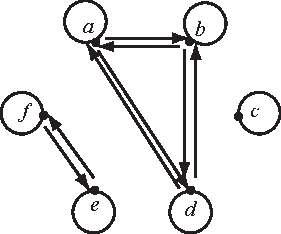
\includegraphics[width=\linewidth]{external/figps-exer2-73.pdf}
\end{image}%
%
\end{divisionsolution}%
\begin{divisionsolution}{3}{}{x:exercise:exer_sec73-2}%
\par\smallskip%
\hypertarget{g:answer:idm818304392-back}{}\quad{}Let \(x \in A\). Since \(x\) has the same number of digits as itself, the relation \(\mathrel{R}\) is reflexive. Now let \(x, y, z \in A\). If \(x \mathrel{R} y\), then \(x\) and \(y\) have the same number of digits. Hence, \(y\) and \(x\) have the same number of digits and \(y \mathrel{R} x\), and so \(\mathrel{R}\) is symmetric.%
\par
If \(x \mathrel{R} y\) and \(y \mathrel{R} z\),then \(x\) and \(y\) have the same number of digits and \(y\)  and  \(z\) have the same number of digits. Hence, \(x\) and \(z\) have the same number of digits, and so \(x \mathrel{R} z\). Therefore, \(\mathrel{R}\) is transitive.%
\par
The equivalence classes are: \(\left\{ 0, 1, 2, \ldots , 9 \right\}\), \(\left\{ 10, 11, 12, \ldots , 99 \right\}\), \(\left\{ 100, 101, 102, \ldots , 999 \right\}\), \(\left\{ 1000 \right\}\).%
\end{divisionsolution}%
\begin{divisionsolution}{4}{}{x:exercise:exer_sec73-congclass}%
\par\smallskip%
\hypertarget{g:answer:idm818286216-back}{}\quad{}The congruence classes for the relation of congruence modulo 5 on the set of integers are%
\begin{align*}
\left[ 0 \right] \amp = \left\{ 5n \mid n \in \mathbb{Z} \right\}\\
\left[ 1 \right] \amp = \left\{ 5n +1 \mid n \in \mathbb{Z} \right\}\\
\left[ 2 \right] \amp = \left\{ 5n + 2 \mid n \in \mathbb{Z} \right\}\\
\left[ 3 \right] \amp = \left\{ 5n + 3 \mid n \in \mathbb{Z} \right\}\\
\left[ 4 \right] \amp = \left\{ 5n + 4 \mid n \in \mathbb{Z} \right\}
\end{align*}
%
\end{divisionsolution}%
\begin{divisionsolution}{5}{}{x:exercise:exer_modpowers}%
\begin{enumerate}[font=\bfseries,label=(\alph*),ref=\alph*]
\item[(a)]\par\smallskip%
\hypertarget{g:answer:idm818291848-back}{}\quad{}Let \(a, b, c \in \Z_9\). Since \(a^2 \equiv a^2 \pmod 9\), we see that \(a \sim a\) and \(\sim\) is reflexive. Let \(a, b, c \in \Z_9\). If \(a \sim b\), then \(a^2 \equiv b^2 \pmod 9\) and hence, by the symmetric property of congruence, \(b^2 \equiv a^2 \pmod 9\). This proves that \(\sim\) is symmetric.  Finally, if \(a \sim b\) and \(b \sim c\), then \(a^2 \equiv b^2 \pmod 9\) and \(b^2 \equiv c^2 \pmod 9\). By the transitive property of congruence, we conclude that \(a^2 \equiv c^2 \pmod 9\) and hence, \(a \sim c\). This proves that \(\sim\) is transitive. The distinct equivalence classes are \(\left\{0, 3, 6 \right\}\), \(\left\{1, 8 \right\}\), \(\left\{ 2, 7 \right\}\), and \(\left\{ 4, 5 \right\}\).%
\end{enumerate}
\end{divisionsolution}%
\begin{divisionsolution}{6}{}{x:exercise:exer_sec73-integer}%
\begin{enumerate}[font=\bfseries,label=(\alph*),ref=\alph*]
\item[(a)]\par\smallskip%
\hypertarget{g:answer:idm818274312-back}{}\quad{}Let \(x \in \left[ \dfrac{5}{7} \right]\). Then \(x - \dfrac{5}{7} \in \Z\), which means that there is an integer \(m\) such that \(x - \dfrac{5}{7} = m\), or \(x = \dfrac{5}{7} + m\). This proves that \(x \in \left\{ \left. m + \dfrac{5}{7} \right| m \in \Z \right\}\) and, hence, that \(\left[ \dfrac{5}{7} \right] \subseteq \left\{ \left. m + \dfrac{5}{7} \right| m 
\in \Z \right\}\). We still need to prove that \(\left\{ \left. m + \dfrac{5}{7} \right| m \in \Z \right\} \subseteq \left[ 
\dfrac{5}{7} \right]\).%
\end{enumerate}
\end{divisionsolution}%
\begin{divisionsolution}{9}{}{x:exercise:exer_sec73-rationals}%
\begin{enumerate}[font=\bfseries,label=(\alph*),ref=\alph*]
\item[(a)]\par\smallskip%
\hypertarget{g:answer:idm818004616-back}{}\quad{}To prove the relation is symmetric, note that if \((a, b) \approx (c, d)\), then \(ad = bc\). This implies that \(cb = da\) and, hence, \((c, d) \approx (a, b)\).%
\item[(c)]\par\smallskip%
\hypertarget{g:answer:idm817994120-back}{}\quad{}\(3a = 2b\)%
\end{enumerate}
\end{divisionsolution}%
\par\medskip
\noindent\textbf{\Large{}7.4\space{}Modular Arithmetic\\
\space{}Exercises}
\begin{divisionsolution}{1}{}{x:exercise:exer_sec74-modtables}%
\begin{enumerate}[font=\bfseries,label=(\alph*),ref=\alph*]
\item[(a)]\par\smallskip%
\hypertarget{g:answer:idm817496472-back}{}\quad{}\begin{center}%
{\tabularfont%
\begin{tabular}{ccccc}
\multicolumn{1}{cB}{\(\oplus\)}&\([ 0 ]\)&\([ 1 ]\)&\([ 2 ]\)&\([ 3 ]\)\tabularnewline\hrulemedium
\multicolumn{1}{cB}{\([ 0 ]\)}&\([ 0 ]\)&\([ 1 ]\)&\([ 2 ]\)&\([ 3 ]\)\tabularnewline[0pt]
\multicolumn{1}{cB}{\([ 1 ]\)}&\([ 1 ]\)&\([ 2 ]\)&\([ 3 ]\)&\([ 0 ]\)\tabularnewline[0pt]
\multicolumn{1}{cB}{\([ 2 ]\)}&\([ 2 ]\)&\([ 3 ]\)&\([ 0 ]\)&\([ 1 ]\)\tabularnewline[0pt]
\multicolumn{1}{cB}{\([ 3 ]\)}&\([ 3 ]\)&\([ 0 ]\)&\([ 1 ]\)&\([ 2 ]\)
\end{tabular}
}%
\end{center}%
%
\par
\begin{center}%
{\tabularfont%
\begin{tabular}{ccccc}
\multicolumn{1}{cB}{\(\odot\)}&\([ 0 ]\)&\([ 1 ]\)&\([ 2 ]\)&\([ 3 ]\)\tabularnewline\hrulemedium
\multicolumn{1}{cB}{\([ 0 ]\)}&\([ 0 ]\)&\([ 0 ]\)&\([ 0 ]\)&\([ 0 ]\)\tabularnewline[0pt]
\multicolumn{1}{cB}{\([ 1 ]\)}&\([ 0 ]\)&\([ 1 ]\)&\([ 2 ]\)&\([ 3 ]\)\tabularnewline[0pt]
\multicolumn{1}{cB}{\([ 2 ]\)}&\([ 0 ]\)&\([ 2 ]\)&\([ 0 ]\)&\([ 2 ]\)\tabularnewline[0pt]
\multicolumn{1}{cB}{\([ 3 ]\)}&\([ 0 ]\)&\([ 3 ]\)&\([ 2 ]\)&\([ 1 ]\)
\end{tabular}
}%
\end{center}%
%
\item[(b)]\par\smallskip%
\hypertarget{g:answer:idm817467416-back}{}\quad{}\begin{center}%
{\tabularfont%
\begin{tabular}{cccccccc}
\multicolumn{1}{cB}{\(\oplus\)}&\([ 0 ]\)&\([ 1 ]\)&\([ 2 ]\)&\([ 3 ]\)&\([ 4 ]\)&\([ 5 ]\)&\([ 6 ]\)\tabularnewline\hrulemedium
\multicolumn{1}{cB}{\([ 0 ]\)}&\([ 0 ]\)&\([ 1 ]\)&\([ 2 ]\)&\([ 3 ]\)&\([ 4 ]\)&\([ 5 ]\)&\([ 6 ]\)\tabularnewline[0pt]
\multicolumn{1}{cB}{\([ 1 ]\)}&\([ 1 ]\)&\([ 2 ]\)&\([ 3 ]\)&\([ 4 ]\)&\([ 5 ]\)&\([ 6 ]\)&\([ 0 ]\)\tabularnewline[0pt]
\multicolumn{1}{cB}{\([ 2 ]\)}&\([ 2 ]\)&\([ 3 ]\)&\([ 4 ]\)&\([ 5 ]\)&\([ 6 ]\)&\([ 0 ]\)&\([ 1 ]\)\tabularnewline[0pt]
\multicolumn{1}{cB}{\([ 3 ]\)}&\([ 3 ]\)&\([ 4 ]\)&\([ 5 ]\)&\([ 6 ]\)&\([ 0 ]\)&\([ 1 ]\)&\([ 2 ]\)\tabularnewline[0pt]
\multicolumn{1}{cB}{\([ 4 ]\)}&\([ 4 ]\)&\([ 5 ]\)&\([ 6 ]\)&\([ 0 ]\)&\([ 1 ]\)&\([ 2 ]\)&\([ 3 ]\)\tabularnewline[0pt]
\multicolumn{1}{cB}{\([ 5 ]\)}&\([ 5 ]\)&\([ 6 ]\)&\([ 0 ]\)&\([ 1 ]\)&\([ 2 ]\)&\([ 3 ]\)&\([ 4 ]\)\tabularnewline[0pt]
\multicolumn{1}{cB}{\([ 6 ]\)}&\([ 6 ]\)&\([ 0 ]\)&\([ 1 ]\)&\([ 2 ]\)&\([ 3 ]\)&\([ 4 ]\)&\([ 5 ]\)
\end{tabular}
}%
\end{center}%
%
\par
\begin{center}%
{\tabularfont%
\begin{tabular}{cccccccc}
\multicolumn{1}{cB}{\(\odot\)}&\([ 0 ]\)&\([ 1 ]\)&\([ 2 ]\)&\([ 3 ]\)&\([ 4 ]\)&\([ 5 ]\)&\([ 6 ]\)\tabularnewline\hrulemedium
\multicolumn{1}{cB}{\([ 0 ]\)}&\([ 0 ]\)&\([ 0 ]\)&\([ 0 ]\)&\([ 0 ]\)&\([ 0 ]\)&\([ 0 ]\)&\([ 0 ]\)\tabularnewline[0pt]
\multicolumn{1}{cB}{\([ 1 ]\)}&\([ 0 ]\)&\([ 1 ]\)&\([ 2 ]\)&\([ 3 ]\)&\([ 4]\)&\([ 5 ]\)&\([ 6 ]\)\tabularnewline[0pt]
\multicolumn{1}{cB}{\([ 2 ]\)}&\([ 0 ]\)&\([ 2 ]\)&\([ 4 ]\)&\([ 6 ]\)&\([ 1 ]\)&\([ 3 ]\)&\([ 5 ]\)\tabularnewline[0pt]
\multicolumn{1}{cB}{\([ 3 ]\)}&\([ 0 ]\)&\([ 3 ]\)&\([ 6 ]\)&\([ 2 ]\)&\([ 5 ]\)&\([ 1 ]\)&\([ 4 ]\)\tabularnewline[0pt]
\multicolumn{1}{cB}{\([ 4 ]\)}&\([ 0 ]\)&\([ 4 ]\)&\([ 1 ]\)&\([ 5 ]\)&\([ 2 ]\)&\([ 6 ]\)&\([ 3 ]\)\tabularnewline[0pt]
\multicolumn{1}{cB}{\([ 5 ]\)}&\([ 0 ]\)&\([ 5 ]\)&\([ 3 ]\)&\([ 1 ]\)&\([ 6 ]\)&\([ 4 ]\)&\([ 2 ]\)\tabularnewline[0pt]
\multicolumn{1}{cB}{\([ 6 ]\)}&\([ 0 ]\)&\([ 6 ]\)&\([ 5 ]\)&\([ 4 ]\)&\([ 3 ]\)&\([ 2 ]\)&\([ 1 ]\)
\end{tabular}
}%
\end{center}%
%
\end{enumerate}
\end{divisionsolution}%
\begin{divisionsolution}{2}{}{x:exercise:exer_sec74-3}%
\begin{enumerate}[font=\bfseries,label=(\alph*),ref=\alph*]
\item[(a)]\par\smallskip%
\hypertarget{g:answer:idm817414424-back}{}\quad{}\([ x ] = [ 1 ]\) or \([ x ] = [ 3 ]\)%
\item[(e)]\par\smallskip%
\hypertarget{g:answer:idm817405464-back}{}\quad{}\([ x ] = [ 2 ]\) or \([ x ] = [ 3 ]\)%
\item[(g)]\par\smallskip%
\hypertarget{g:answer:idm817397144-back}{}\quad{}The equation has no solution.%
\end{enumerate}
\end{divisionsolution}%
\begin{divisionsolution}{3}{}{x:exercise:exer_sec74-4}%
\begin{enumerate}[font=\bfseries,label=(\alph*),ref=\alph*]
\item[(a)]\par\smallskip%
\hypertarget{g:answer:idm817397400-back}{}\quad{}The statement is false. By using the multiplication table for \(\mathbb{Z}_6\), we see that a counterexample is \(\left[ a \right] = \left[ 2 \right]\).%
\item[(b)]\par\smallskip%
\hypertarget{g:answer:idm817396248-back}{}\quad{}The statement is true. By using the multiplication table for \(\mathbb{Z}_5\), we see that:%
\begin{align*}
\left[ 1 \right] \amp \odot \left[ 1 \right] = \left[ 1 \right]. \amp 
\left[ 2 \right] \amp \odot \left[ 3 \right] = \left[ 1 \right]\\
\left[ 3 \right] \amp \odot \left[ 2 \right] = \left[ 1 \right]. \amp 
\left[ 4 \right] \amp \odot \left[ 4 \right] = \left[ 1 \right]
\end{align*}
%
\end{enumerate}
\end{divisionsolution}%
\begin{divisionsolution}{5}{}{x:exercise:exer_squaresinZ5}%
\begin{enumerate}[font=\bfseries,label=(\alph*),ref=\alph*]
\item[(a)]\par\smallskip%
\hypertarget{g:answer:idm817377560-back}{}\quad{}The proof consists of the following computations:%
\begin{align*}
[ 1 ]^2 \amp = [ 1 ]\\
[ 2 ]^2 \amp = [ 4 ]\\
[ 3 ]^2 \amp = [ 9 ] = [ 4 ]\\
[ 4 ]^2 \amp = [ 16 ] = [ 1 ]
\end{align*}
%
\end{enumerate}
\end{divisionsolution}%
\begin{divisionsolution}{17}{}{x:exercise:exer_sec74cong3}%
\begin{enumerate}[font=\bfseries,label=(\alph*),ref=\alph*]
\item[(a)]\par\smallskip%
\hypertarget{g:answer:idm817337624-back}{}\quad{}Prove the contrapositive by calculating \([ a ]^2 + [ b ]^2\) for all nonzero \([ a ]\) and \([ b ]\) in \(\Z_3\).%
\end{enumerate}
\end{divisionsolution}%
\begin{divisionsolution}{19}{}{x:exercise:exer_sec74-15}%
\par\smallskip%
\noindent\textbf{\blocktitlefont Hint}.\hypertarget{g:hint:idm817322648-back}{}\quad{}What are the possible values of \(n\) (mod 8)?%
\end{divisionsolution}%
\par\medskip
\noindent\textbf{\Large{}8\space{}Topics in Number Theory\\
8.1\space{}The Greatest Common Divisor\\
\space{}Exercises}
\begin{divisionsolution}{1}{}{x:exercise:exer_sec81-1}%
\begin{enumerate}[font=\bfseries,label=(\alph*),ref=\alph*]
\item[(a)]\par\smallskip%
\hypertarget{g:answer:idm816928808-back}{}\quad{}The set of positive common divisors of 21 and 28 is \(\{1, 7\}\). So \(\gcd ( {21, 28} ) = 7\).%
\item[(b)]\par\smallskip%
\hypertarget{g:answer:idm816927144-back}{}\quad{}The set of positive common divisors of \(-21\) and 28 is \(\{1, 7\}\). So \(\gcd ( { - 21, 28} ) = 7\).%
\item[(c)]\par\smallskip%
\hypertarget{g:answer:idm816927784-back}{}\quad{}The set of positive common divisors of 58 and 63 is \(\{1 \}\). So \(\gcd ( {58, 63} ) = 1\).%
\item[(d)]\par\smallskip%
\hypertarget{g:answer:idm816931496-back}{}\quad{}The set of positive common divisors of 0 and 12 is \(\{1, 2, 3, 4, 6, 12 \}\). So \(\gcd ( {0, 12} ) = 12\).%
\end{enumerate}
\end{divisionsolution}%
\begin{divisionsolution}{2}{}{x:exercise:exer_sec81-2}%
\begin{enumerate}[font=\bfseries,label=(\alph*),ref=\alph*]
\item[(a)]\par\smallskip%
\noindent\textbf{\blocktitlefont Hint}.\hypertarget{g:hint:idm816918440-back}{}\quad{}Prove that \(k \mid \left[ ( {a+1} ) - a \right]\).%
\end{enumerate}
\end{divisionsolution}%
\begin{divisionsolution}{4}{}{x:exercise:exer_sec81-props}%
\begin{enumerate}[font=\bfseries,label=(\alph*),ref=\alph*]
\item[(a)]\par\smallskip%
\hypertarget{g:answer:idm816908840-back}{}\quad{}\(|b|\) is the largest natural number that divides 0 and \(b\).%
\item[(b)]\par\smallskip%
\hypertarget{g:answer:idm816907560-back}{}\quad{}The integers \(b\) and \(-b\) have the same divisors.  Therefore, \(\gcd ( a, -b ) = \gcd ( a, b )\).%
\end{enumerate}
\end{divisionsolution}%
\begin{divisionsolution}{5}{}{x:exercise:exer_sec81-4}%
\begin{enumerate}[font=\bfseries,label=(\alph*),ref=\alph*]
\item[(a)]\par\smallskip%
\hypertarget{g:answer:idm816902824-back}{}\quad{}\(\gcd ( {36, 60} ) = 12\), \(12 = 36 \cdot 2 + 60 \cdot ( { - 1} )\)%
\item[(b)]\par\smallskip%
\hypertarget{g:answer:idm816898856-back}{}\quad{}\(\gcd ( {901, 935} ) = 17\), \(17 = 901 \cdot 27 + 935 \cdot ( { - 26} )\)%
\item[(e)]\par\smallskip%
\hypertarget{g:answer:idm816899496-back}{}\quad{}\(\gcd ( {901, -935} ) = 17\), \(17 = 901 \cdot 27 + (-935) \cdot ( { 26} )\)%
\end{enumerate}
\end{divisionsolution}%
\begin{divisionsolution}{6}{}{x:exercise:exer81_solvingeqn}%
\begin{enumerate}[font=\bfseries,label=(\alph*),ref=\alph*]
\item[(a)]\par\smallskip%
\hypertarget{g:answer:idm816887592-back}{}\quad{}One possibility is \(u = -3\) and \(v = 2\).  In this case, \(9u + 14v = 1\). We then multiply both sides of this equation by 10 to obtain%
\begin{equation*}
9 \cdot (-30) + 14 \cdot 20 = 10\text{.}
\end{equation*}
So we can use \(x = -30\) and \(y = 20\).%
\end{enumerate}
\end{divisionsolution}%
\begin{divisionsolution}{7}{}{x:exercise:exer_gcdandfractions}%
\begin{enumerate}[font=\bfseries,label=(\alph*),ref=\alph*]
\item[(a)]\par\smallskip%
\hypertarget{g:answer:idm816875304-back}{}\quad{}\(11 \cdot (-3) + 17 \cdot 2 = 1\)%
\item[(b)]\par\smallskip%
\hypertarget{g:answer:idm816880552-back}{}\quad{}\(\dfrac{m}{11} + \dfrac{n}{17} = \dfrac{17m +11n}{187}\)%
\item[(c)]\par\smallskip%
\noindent\textbf{\blocktitlefont Hint}.\hypertarget{g:hint:idm816877352-back}{}\quad{}Write the rational numbers in the form \(\dfrac{m}{{11}}\)  and  \(\dfrac{n}{{17}}\), where  \(m, n \in \mathbb{Z}\). Then write%
\begin{equation*}
\frac{m}{{11}} + \frac{n}{{17}} = \frac{{10}}{{187}}\text{.}
\end{equation*}
Use \hyperref[x:task:exer_gcdanddena]{Task~{\xreffont 7}.{\xreffont\ref{x:task:exer_gcdanddena}}, p.\,\pageref{x:task:exer_gcdanddena}} and \hyperref[x:task:exer_gcdanddenb]{Task~{\xreffont 7}.{\xreffont\ref{x:task:exer_gcdanddenb}}, p.\,\pageref{x:task:exer_gcdanddenb}} to determine \(m\)  and  \(n\).%
\end{enumerate}
\end{divisionsolution}%
\par\medskip
\noindent\textbf{\Large{}8.2\space{}Prime Numbers and Prime Factorizations\\
\space{}Exercises}
\begin{divisionsolution}{1}{}{x:exercise:exer_sec82-1}%
\begin{enumerate}[font=\bfseries,label=(\alph*),ref=\alph*]
\item[(a)]\par\smallskip%
\noindent\textbf{\blocktitlefont Hint}.\hypertarget{g:hint:idm816609560-back}{}\quad{}Use the fact that the only natural number divisors of a prime number \(p\) are 1 and \(p\).%
\item[(b)]\par\smallskip%
\noindent\textbf{\blocktitlefont Hint}.\hypertarget{g:hint:idm816611992-back}{}\quad{}Use the fact that the only natural number divisors of a prime number \(p\) are 1 and \(p\).%
\end{enumerate}
\end{divisionsolution}%
\begin{divisionsolution}{2}{}{x:exercise:exer_sec82-2}%
\par\smallskip%
\noindent\textbf{\blocktitlefont Hint}.\hypertarget{g:hint:idm816603800-back}{}\quad{}Consider two cases: (1) \(p \mid a\); and (2) \(p\) does not divide \(a\).%
\par\smallskip%
\hypertarget{g:answer:idm816602392-back}{}\quad{}Use cases: (1) \(p\) divides \(a\); (2) \(p\) does not divide \(a\). In the first case, the conclusion is automatically true. For the second case, use the fact that \(\gcd ( p, a ) = 1\) and so we can use \hyperref[x:theorem:T_relativelyprimeprop]{Theorem~{\xreffont\ref{x:theorem:T_relativelyprimeprop}}, p.\,\pageref{x:theorem:T_relativelyprimeprop}} to conclude that \(p\) divides \(b\). Another option is to write the number 1 as a linear combination of \(a\) and \(p\) and then multiply both sides of the equation by \(b\).%
\end{divisionsolution}%
\begin{divisionsolution}{3}{}{x:exercise:exer_sec82-3}%
\par\smallskip%
\noindent\textbf{\blocktitlefont Hint}.\hypertarget{g:hint:idm816592920-back}{}\quad{}A hint for the inductive step: Write \(p \mid ( {a_1 a_2  \cdots a_m } )a_{m + 1}\). Then look at two cases: (1) \(p \mid a_{m + 1}\); (2) \(p\) does not divide \(a_{m + 1}\).%
\end{divisionsolution}%
\begin{divisionsolution}{4}{}{x:exercise:exer_lincombequalone}%
\begin{enumerate}[font=\bfseries,label=(\alph*),ref=\alph*]
\item[(a)]\par\smallskip%
\hypertarget{g:answer:idm816591640-back}{}\quad{}\(\gcd ( a, b ) = 1\). Why?%
\item[(b)]\par\smallskip%
\hypertarget{g:answer:idm816582808-back}{}\quad{}\(\gcd ( a, b ) = 1\) or \(\gcd ( a, b ) = 2\). Why?%
\end{enumerate}
\end{divisionsolution}%
\begin{divisionsolution}{7}{}{x:exercise:exer_gcd-divbyd}%
\begin{enumerate}[font=\bfseries,label=(\alph*),ref=\alph*]
\item[(a)]\par\smallskip%
\hypertarget{g:answer:idm816575000-back}{}\quad{}\(\gcd \left( 16, 28 \right) = 4\). Also, \(\dfrac{16}{4} = 4\), \(\dfrac{28}{4} = 7\), and \(\gcd \left( 4, 7 \right) = 1\).%
\item[(b)]\par\smallskip%
\hypertarget{g:answer:idm816575384-back}{}\quad{}\(\gcd \left( 10, 45 \right) = 5\). Also, \(\dfrac{10}{5} = 2\), \(\dfrac{45}{5} = 9\), and \(\gcd \left( 2, 9 \right) = 1\).%
\item[(c)]\par\smallskip%
\noindent\textbf{\blocktitlefont Hint}.\hypertarget{g:hint:idm816569368-back}{}\quad{}Start by writing \(d\) as a linear combination of \(a\) and \(b\).%
\end{enumerate}
\end{divisionsolution}%
\begin{divisionsolution}{9}{}{x:exercise:exer_24divides-nsquaredminus1}%
\par\smallskip%
\noindent\textbf{\blocktitlefont Hint}.\hypertarget{g:hint:idm816557848-back}{}\quad{}\hyperref[x:task:exer_sec82-truefalseb]{Task~{\xreffont 8}.{\xreffont\ref{x:task:exer_sec82-truefalseb}}, p.\,\pageref{x:task:exer_sec82-truefalseb}} of \hyperlink{x:exercise:exer_sec82-truefalse}{Exercise~{\xreffont 8}, p.\,\pageref{x:exercise:exer_sec82-truefalse}} can be helpful.%
\end{divisionsolution}%
\begin{divisionsolution}{11}{}{g:exercise:idm816554392}%
\par\smallskip%
\hypertarget{g:answer:idm816542104-back}{}\quad{}The statement is true. Start of a proof: If  \(\gcd ( {a, b} ) = 1\) and \(c \mid ( {a + b} )\), then there exist integers \(x\) and \(y\) such that \(ax + by = 1\) and there exists an integer \(m\) such that \(a + b = cm\).%
\end{divisionsolution}%
\begin{divisionsolution}{16}{}{g:exercise:idm816532504}%
\begin{enumerate}[font=\bfseries,label=(\alph*),ref=\alph*]
\item[(b)]\par\smallskip%
\noindent\textbf{\blocktitlefont Hint}.\hypertarget{g:hint:idm816524696-back}{}\quad{}Try setting up cases using congruence modulo 3.%
\end{enumerate}
\end{divisionsolution}%
\begin{divisionsolution}{17}{}{g:exercise:idm816527000}%
\par\smallskip%
\noindent\textbf{\blocktitlefont Hint}.\hypertarget{g:hint:idm816525592-back}{}\quad{}One way is to start by writing 1 as a linear combination of \(a\) and \(n\).%
\end{divisionsolution}%
\begin{divisionsolution}{18}{}{x:exercise:exer_sec82-twinprimes}%
\par\smallskip%
\noindent\textbf{\blocktitlefont Hint}.\hypertarget{g:hint:idm816514840-back}{}\quad{}Look at several examples of twin primes. What do you notice about the number that is between the two twin primes? Set up cases based on this observation.%
\end{divisionsolution}%
\par\medskip
\noindent\textbf{\Large{}8.3\space{}Linear Diophantine Equations}
\par\medskip
\noindent\textbf{\large{}{}Exercises}
\begin{divisionsolution}{8.3.3}{}{x:exercise:exer_sec83-2}%
\begin{enumerate}[font=\bfseries,label=(\alph*),ref=\alph*]
\item[(a)]\par\smallskip%
\hypertarget{g:answer:idm816247080-back}{}\quad{}\(x = -3 + 14k\), \(y = 2 - 9k\)%
\item[(b)]\par\smallskip%
\hypertarget{g:answer:idm816243880-back}{}\quad{}\(x = -1 + 11k\), \(y = 1 - 9k\)%
\item[(c)]\par\smallskip%
\hypertarget{g:answer:idm816243752-back}{}\quad{}No solution%
\item[(d)]\par\smallskip%
\hypertarget{g:answer:idm816239528-back}{}\quad{}\(x = 2+3k\), \(y = -2-4k\)%
\end{enumerate}
\end{divisionsolution}%
\begin{divisionsolution}{8.3.4}{}{x:exercise:exer_balancing}%
\par\smallskip%
\noindent\textbf{\blocktitlefont Hint}.\hypertarget{g:hint:idm816228264-back}{}\quad{}Notice that \(\gcd( {50, 27} ) = 1\). Start by writing 1 as a linear combination of 50 and 27.%
\par\smallskip%
\hypertarget{g:answer:idm816229160-back}{}\quad{}There are several possible solutions to this problem, each of which can be generated from the solutions of the Diophantine equation \(27x + 50y = 25\).%
\end{divisionsolution}%
\begin{divisionsolution}{8.3.5}{}{x:exercise:exer_sec83-5}%
\par\smallskip%
\hypertarget{g:answer:idm816234920-back}{}\quad{}This problem can be solved by finding all solutions of a linear Diophantine equation \(25x + 16y = 1461\), where both \(x\) and \(y\) are positive. The mininum number of people attending the banquet is 66.%
\end{divisionsolution}%
\begin{divisionsolution}{8.3.6}{}{x:exercise:exer_lindioph3}%
\begin{enumerate}[font=\bfseries,label=(\alph*),ref=\alph*]
\item[(a)]\par\smallskip%
\hypertarget{g:answer:idm816235176-back}{}\quad{}\(y = 12 + 16k, x_3 = -1 - 3k\)%
\item[(b)]\par\smallskip%
\hypertarget{g:answer:idm816223016-back}{}\quad{}If \(3y = 12x_1 + 9x_2\) and \(3y + 16x_3 = 20\), we can substitute for \(3y\) and obtain \(12x_1 + 9x_2 + 16x_3 = 20\).%
\item[(c)]\par\smallskip%
\hypertarget{g:answer:idm816220584-back}{}\quad{}Rewrite the equation \(12x_1 + 9x_2 = 3y\) as \(4x_1 + 3x_2 = y\). A general solution for this linear Diophantine equation is%
\begin{align*}
x_1 \amp = y + 3n\\
x_2 \amp = -y - 4n\text{.}
\end{align*}
%
\end{enumerate}
\end{divisionsolution}%
\par\medskip
\noindent\textbf{\Large{}9\space{}Finite and Infinite Sets\\
9.1\space{}Finite Sets\\
\space{}Exercises}
\begin{divisionsolution}{2}{}{x:exercise:exer_sec92-1}%
\par\smallskip%
\hypertarget{g:answer:idm815919768-back}{}\quad{}One way to do this is to prove that the following function is a bijection: \(f\x A \times \left\{ x \right\} \to A\) by \(f ( a, x ) = a\), for all \(( a, x ) \in A \times \left\{ x \right\}\).%
\end{divisionsolution}%
\begin{divisionsolution}{3}{}{x:exercise:exer91_evennaturals}%
\par\smallskip%
\hypertarget{g:answer:idm815922584-back}{}\quad{}One way to prove that \(\N \approx E^+\) is to find a bijection from \(\N\) to \(E^+\). One possibility is \(f: \mathbb{N} \to E^+\) by \(f \left( n \right) = 2n\) for all \(n \in \mathbb{N}\). (We must prove that this is a bijection.)%
\end{divisionsolution}%
\begin{divisionsolution}{4}{}{x:exercise:exer_sec92corollary}%
\par\smallskip%
\noindent\textbf{\blocktitlefont Hint}.\hypertarget{g:hint:idm815913752-back}{}\quad{}One approach is to use the fact that \(A = \left( A - \left\{ x \right\} \right) \cup 
\left\{x \right\}\).%
\par\smallskip%
\hypertarget{g:answer:idm815913496-back}{}\quad{}Notice that \(A = ( A - \left\{ x \right\} ) \cup \left\{x \right\}\). Use \hyperref[x:theorem:T_finitesubsets]{Theorem~{\xreffont\ref{x:theorem:T_finitesubsets}}, p.\,\pageref{x:theorem:T_finitesubsets}} to conclude that \(A - \left\{ x \right\}\) is finite. Then use \hyperref[x:lemma:L_addone]{Lemma~{\xreffont\ref{x:lemma:L_addone}}, p.\,\pageref{x:lemma:L_addone}}.%
\end{divisionsolution}%
\begin{divisionsolution}{5}{}{x:exercise:exer_sec92-finitesets}%
\begin{enumerate}[font=\bfseries,label=(\alph*),ref=\alph*]
\item[(a)]\par\smallskip%
\hypertarget{g:answer:idm815915160-back}{}\quad{}Since \(A \cap B \subseteq A\), if \(A\) is finite, then \hyperref[x:theorem:T_finitesubsets]{Theorem~{\xreffont\ref{x:theorem:T_finitesubsets}}, p.\,\pageref{x:theorem:T_finitesubsets}} implies that \(A \cap B\) is finite.%
\item[(b)]\par\smallskip%
\hypertarget{g:answer:idm815907480-back}{}\quad{}The sets \(A\) and \(B\) are subsets of \(A \cup B\). So if \(A \cup B\) is finite, then \(A\) and \(B\) are finite.%
\end{enumerate}
\end{divisionsolution}%
\begin{divisionsolution}{7}{}{x:exercise:exer_sec92-7}%
\begin{enumerate}[font=\bfseries,label=(\alph*),ref=\alph*]
\item[(a)]\par\smallskip%
\noindent\textbf{\blocktitlefont Hint}.\hypertarget{g:hint:idm815895704-back}{}\quad{}Since \(A \approx B\) and \(C \approx D\), there exist bijections \(f:A \to B\) and \(g:C \to D\). To prove that \(A \times C \approx B \times D\), prove that \(h:A \times C \to B \times D\) is a bijection, where \(h ( a, c ) = \left( f ( a ), g ( c ) \right)\), for all \(( a, c ) \in A \times C\).%
\par\smallskip%
\hypertarget{g:answer:idm815890712-back}{}\quad{}Remember that two ordered pairs are equal if and only if their corresponding coordinates are equal. So if \(\left( a_1, c_1 \right) , \left( a_2, c_2 \right) 
\in A \times C\) and \(h \left( a_1, c_1 \right) = h \left( a_2, c_2 \right)\), then \(\left( f \left( a_1 \right), g \left( c_1 \right) \right) =
\left( f \left( a_2 \right), g \left( c_2 \right) \right)\). We can then conclude that \(f \left( a_1 \right) = f \left( a_2 \right)\) and \(g \left( c_1 \right) = g \left( c_2 \right)\). Since \(f\) and \(g\) are both injections, this means that \(a_1 = a_2\) and \(c_1 = c_2\) and therefore, \(\left( a_1, c_1 \right) = \left( a_2, c_2 \right)\). This proves that \(f\) is an injection. Now let \(\left( b, d \right) \in B \times D\). Since \(f\) and \(g\) are surjections, there exists \(a \in A\) and \(c \in C\) such that \(f \left( a \right) = b\) and \(g \left( c \right) = d\). Therefore, \(h \left( a, c \right) = \left( b, d \right)\). This proves that \(f\) is a surjection.%
\end{enumerate}
\end{divisionsolution}%
\begin{divisionsolution}{8}{}{x:exercise:exer_sec927}%
\begin{enumerate}[font=\bfseries,label=(\alph*),ref=\alph*]
\item[(a)]\par\smallskip%
\hypertarget{g:answer:idm815876248-back}{}\quad{}If we define the function \(f\) by \(f ( 1 ) = a\), \(f ( 2 ) = b\), \(f ( 3 ) = c\), \(f ( 4 ) = a\), and \(f ( 5 ) = b\), then we can use \(g ( a ) = 1\), \(g ( b ) = 2\), and \(g ( 3 ) = c\). The function \(g\) is an injection.%
\end{enumerate}
\end{divisionsolution}%
\begin{divisionsolution}{10}{}{g:exercise:idm815861656}%
\par\smallskip%
\noindent\textbf{\blocktitlefont Hint}.\hypertarget{g:hint:idm815862296-back}{}\quad{}Since \(B\) is finite, there exists a natural number \(m\) such that \(\mathbb{N}_m \approx B\). This means there exists a bijection \(k:\mathbb{N}_m \to B\). Now let \(h = k \circ g\), where \(g\) is the function constructed in \hyperlink{x:exercise:exer_sec928}{Exercise~{\xreffont 9}, p.\,\pageref{x:exercise:exer_sec928}}.%
\end{divisionsolution}%
\par\medskip
\noindent\textbf{\Large{}9.2\space{}Countable Sets\\
\space{}Exercises}
\begin{divisionsolution}{1}{}{x:exercise:exer_sec93-1}%
\begin{enumerate}[font=\bfseries,label=(\alph*),ref=\alph*]
\item[(a)]\par\smallskip%
\hypertarget{g:answer:idm815556632-back}{}\quad{}True.%
\item[(b)]\par\smallskip%
\hypertarget{g:answer:idm815550360-back}{}\quad{}True.%
\item[(c)]\par\smallskip%
\hypertarget{g:answer:idm815551768-back}{}\quad{}True.%
\item[(d)]\par\smallskip%
\hypertarget{g:answer:idm815550104-back}{}\quad{}False.%
\end{enumerate}
\end{divisionsolution}%
\begin{divisionsolution}{2}{}{x:exercise:exer_sec93-2}%
\begin{enumerate}[font=\bfseries,label=(\alph*),ref=\alph*]
\item[(a)]\par\smallskip%
\hypertarget{g:answer:idm815553432-back}{}\quad{}Prove that the function \(f: \mathbb{N} \to F^+\) defined by \(f \left( n \right) = 5n\) for all \(n \in \mathbb{N}\) is a bijection.%
\item[(e)]\par\smallskip%
\hypertarget{g:answer:idm815544216-back}{}\quad{}One way is to define \(f\x \N \to \N -\{4, 5, 6 \}\) by%
\begin{equation*}
f( n ) = \begin{cases}n \amp \text{ if \(n = 1\), \(n = 2\), or \(n = 3\) } \\ 
f ( n + 3 )  \amp \text{ if \(n \geq 4\) } . \end{cases}
\end{equation*}
and then prove that the function \(f\) is a bijection. It is also possible to use \hyperref[x:corollary:C_subsetofcountable]{Corollary~{\xreffont\ref{x:corollary:C_subsetofcountable}}, p.\,\pageref{x:corollary:C_subsetofcountable}} to conclude that \(\mathbb{N} - \left\{ 4, 5, 6 \right\}\) is countable, but it must also be proved that \(\mathbb{N} - \left\{ 4, 5, 6 \right\}\) cannot be finite. To do this, assume that \(\mathbb{N} - \left\{ 4, 5, 6 \right\}\) is finite and then prove that \(\N\) is finite, which is a contradiction.%
\item[(f)]\par\smallskip%
\hypertarget{g:answer:idm815542936-back}{}\quad{}Let \(A = \left\{ m \in \mathbb{Z} \mid m \equiv 2 \pmod 3 \right\} 
= \left\{ 3k + 2 \mid k \in \mathbb{Z} \right\}\). Prove that the function \(f: \mathbb{Z} \to A\) is a bijection, where \(f \left( x \right) = 3x + 2\) for all \(x \in \mathbb{Z}\). This proves that \(\mathbb{Z} \approx A\) and hence, \(\mathbb{N} \approx A\).%
\end{enumerate}
\end{divisionsolution}%
\begin{divisionsolution}{3}{}{x:exercise:exer_subsetisinfinite}%
\par\smallskip%
\noindent\textbf{\blocktitlefont Hint}.\hypertarget{g:hint:idm815538584-back}{}\quad{}Let \(A\) and \(B\) be sets. If \(A\) is infinite and \(A \subseteq B\), then \(B\) is infinite.%
\par\smallskip%
\hypertarget{g:answer:idm815533080-back}{}\quad{}For each \(n \in \mathbb{N}\), let \(P ( n )\) be ``If \(\text{ card} ( B ) = n\), then \(A \cup B\) is a countably infinite set.''%
\par
Note that if \(\text{ card} ( B ) = k+1\) and \(x \in B\), then \(\text{ card} ( B - \left\{ x \right\} ) = k\). Apply the inductive assumption to \(B - \left\{ x \right\}\).%
\end{divisionsolution}%
\begin{divisionsolution}{5}{}{x:exercise:exer_addfinitetocountable}%
\par\smallskip%
\noindent\textbf{\blocktitlefont Hint}.\hypertarget{g:hint:idm815523736-back}{}\quad{}Let \(\text{ card} ( B ) = n\) and use a proof by induction on \(n\). \hyperref[x:theorem:T_addonetocountable]{Theorem~{\xreffont\ref{x:theorem:T_addonetocountable}}, p.\,\pageref{x:theorem:T_addonetocountable}} is the basis step.%
\end{divisionsolution}%
\begin{divisionsolution}{6}{}{x:exercise:exer_unionofcountable}%
\par\smallskip%
\hypertarget{g:answer:idm815523096-back}{}\quad{}Let \(m, n \in \mathbb{N}\) and assume that \(h \left( n \right) = h \left( m \right)\). Then since \(A\) and \(B\) are disjoint, either \(h \left( n \right)\) and \(h \left( m \right)\) are both in \(A\) or are both in \(B\). If they are both in \(A\), then both \(m\) and \(n\) are odd and%
\begin{equation*}
f \left( \frac{n + 1}{2} \right) = h \left( n \right) = h \left( m \right) = f \left( \frac{m + 1}{2} \right)\text{.}
\end{equation*}
Since \(f\) is an injection, this implies that \(\dfrac{n + 1}{2} = \dfrac{m + 1}{2}\) and hence that \(n = m\). Similary, if both \(h \left( n \right)\) and \(h \left( m \right)\) are in \(B\), then \(m\) and \(n\) are even and \(g \left( \dfrac{n}{2} \right) = g \left( \dfrac{m}{2} \right)\), and since \(g\) is an injection, \(\dfrac{n}{2} = \dfrac{m}{2}\) and \(n = m\). Therefore, \(h\) is an injection.%
\par
Now let \(y \in A \cup B\). There are only two cases to consider: \(y \in A\) or \(y \in B\). If \(y \in A\), then since \(f\) is a surjection, there exists an \(m \in \mathbb{N}\) such that \(f \left( m \right) = y\). Let \(n = 2m - 1\). Then \(n\) is an odd natural number, \(m = \dfrac{n + 1}{2}\), and%
\begin{equation*}
h \left( n \right) = f \left( \frac{n + 1}{2} \right) = f \left( m \right) = y\text{.}
\end{equation*}
Now assume \(y \in B\) and use the fact that \(g\) is a surjection to help prove that there exists a natural number \(n\) such that \(h(n) = y\). We can then conclude that \(h\) is a surjection.%
\end{divisionsolution}%
\begin{divisionsolution}{7}{}{x:exercise:exer_Qiscountable}%
\par\smallskip%
\noindent\textbf{\blocktitlefont Hint}.\hypertarget{g:hint:idm815357848-back}{}\quad{}Use \hyperref[x:theorem:T_addonetocountable]{Theorem~{\xreffont\ref{x:theorem:T_addonetocountable}}, p.\,\pageref{x:theorem:T_addonetocountable}} and \hyperref[x:theorem:T_unionofcountable]{Theorem~{\xreffont\ref{x:theorem:T_unionofcountable}}, p.\,\pageref{x:theorem:T_unionofcountable}}.%
\par\smallskip%
\hypertarget{g:answer:idm815358360-back}{}\quad{}By \hyperref[x:theorem:T_positiverationals]{Theorem~{\xreffont\ref{x:theorem:T_positiverationals}}, p.\,\pageref{x:theorem:T_positiverationals}}, the set \(\mathbb{Q}^+\) of positive rational numbers is countably infinite. So by \hyperref[x:theorem:T_addonetocountable]{Theorem~{\xreffont\ref{x:theorem:T_addonetocountable}}, p.\,\pageref{x:theorem:T_addonetocountable}}, \(\mathbb{Q}^+ \cup \left\{ 0 \right\}\) is countably infinite. Now prove that the set \(\mathbb{Q}^-\) of all negative rational numbers is countably infinite and then use \hyperref[x:theorem:T_unionofcountable]{Theorem~{\xreffont\ref{x:theorem:T_unionofcountable}}, p.\,\pageref{x:theorem:T_unionofcountable}} to prove that \(\mathbb{Q}\) is countably infinite.%
\end{divisionsolution}%
\begin{divisionsolution}{8}{}{x:exercise:exer_countinf-finite}%
\par\smallskip%
\hypertarget{g:answer:idm815352472-back}{}\quad{}Since \(A - B \subseteq A\), the set \(A - B\) is countable. Now assume \(A - B\) is finite and show that this leads to a contradiction.%
\end{divisionsolution}%
\begin{divisionsolution}{9}{}{x:exercise:exer_NxNbijection}%
\begin{enumerate}[font=\bfseries,label=(\alph*),ref=\alph*]
\item[(a)]\par\smallskip%
\noindent\textbf{\blocktitlefont Hint}.\hypertarget{g:hint:idm815348376-back}{}\quad{}If \(f ( m, n ) = f ( s, t )\), there are three cases to consider: \(m > s\), \(m \lt s\), and \(m = s\). Use laws of exponents to prove that the first two cases lead to a contradiction.%
\item[(b)]\par\smallskip%
\noindent\textbf{\blocktitlefont Hint}.\hypertarget{g:hint:idm815343768-back}{}\quad{}You may use the fact that if \(y \in \mathbb{N}\), then \(y = 2^k x\), where \(x\) is an odd natural number and \(k\) is a non-negative integer. This is actually a consequence of the Fundamental Theorem of Arithmetic, \hyperref[x:theorem:T_fundtheorem]{Theorem~{\xreffont\ref{x:theorem:T_fundtheorem}}, p.\,\pageref{x:theorem:T_fundtheorem}}. [See \hyperlink{x:exercise:exer_fundtheoremcons}{Exercise~{\xreffont 13}, p.\,\pageref{x:exercise:exer_fundtheoremcons}} in \hyperref[x:section:S_primefactorizations]{Section~{\xreffont\ref{x:section:S_primefactorizations}}, p.\,\pageref{x:section:S_primefactorizations}}.]%
\end{enumerate}
\end{divisionsolution}%
\begin{divisionsolution}{11}{}{x:exercise:exer_subsetofN}%
\par\smallskip%
\noindent\textbf{\blocktitlefont Hint}.\hypertarget{g:hint:idm815338648-back}{}\quad{}To prove that \(g\) is an injection, it might be easier to prove that for all \(r, s \in \mathbb{N}\), if \(r \ne s\), then \(g ( r ) \ne g ( s )\). To do this, we may assume that \(r \lt s\) since one of the two numbers must be less than the other. Then notice that \(g ( r ) \in \left\{ g( 1 ), g( 2 ), \ldots,
g( s-1 ) \right\}\). To prove that \(g\) is a surjection, let \(b \in B\) and notice that for some \(k \in \mathbb{N}\), there will be \(k\) natural numbers in \(B\) that are less than \(b\).%
\end{divisionsolution}%
\begin{divisionsolution}{12}{}{x:exercise:exer_subsetofcountable}%
\par\smallskip%
\noindent\textbf{\blocktitlefont Hint}.\hypertarget{g:hint:idm815331992-back}{}\quad{}Let \(S\) be a countable set and assume that \(A \subseteq S\). There are two cases: \(A\) is finite or \(A\) is infinite. If \(A\) is infinite, let \(f\x S \to \mathbb{N}\) be a bijection and define \(g\x A \to f ( A )\) by \(g ( x ) = f ( x )\), for each \(x \in A\).%
\end{divisionsolution}%
\par\medskip
\noindent\textbf{\Large{}9.3\space{}Uncountable Sets\\
\space{}Exercises}
\begin{divisionsolution}{1}{}{x:exercise:exer_sec94-1}%
\begin{enumerate}[font=\bfseries,label=(\alph*),ref=\alph*]
\item[(a)]\par\smallskip%
\hypertarget{g:answer:idm815096088-back}{}\quad{}One such bijection is \(f\x ( 0, \infty ) \to \mathbb{R}\) by \(f ( x ) = \ln x\) for all \(x \in ( 0, \infty )\)%
\item[(b)]\par\smallskip%
\hypertarget{g:answer:idm815001496-back}{}\quad{}One such bijection is \(g\x ( 0, \infty ) \to ( a, \infty )\) by \(g( x ) = x + a\) for all \(x \in ( 0, \infty )\). The function \(g\) is a bijection and so \(\left( 0, \infty \right) \approx \left( a, \infty \right)\). Then use Part~(a).%
\end{enumerate}
\end{divisionsolution}%
\begin{divisionsolution}{2}{}{x:exercise:exer_irrationaluncount}%
\par\smallskip%
\hypertarget{g:answer:idm815002648-back}{}\quad{}Use a proof by contradiction. Let \(\mathbb{H}\) be the set of irrational numbers and assume that \(\mathbb{H}\) is countable. Then \(\mathbb{R} = \mathbb{Q} \cup \mathbb{H}\) and \(\mathbb{Q}\) and \(\mathbb{H}\) are disjoint. Use \hyperref[x:theorem:T_unionofcountable]{Theorem~{\xreffont\ref{x:theorem:T_unionofcountable}}, p.\,\pageref{x:theorem:T_unionofcountable}}, to obtain a contradiction.%
\end{divisionsolution}%
\begin{divisionsolution}{3}{}{x:exercise:exer_supersetofuncount}%
\par\smallskip%
\hypertarget{g:answer:idm814993560-back}{}\quad{}By \hyperref[x:corollary:C_subsetofcountable]{Corollary~{\xreffont\ref{x:corollary:C_subsetofcountable}}, p.\,\pageref{x:corollary:C_subsetofcountable}}, every subset of a countable set is countable. So if \(B\) is countable, then \(A\) is countable.%
\end{divisionsolution}%
\begin{divisionsolution}{4}{}{x:exercise:exer93_uncountablesets}%
\par\smallskip%
\hypertarget{g:answer:idm814996760-back}{}\quad{}By Cantor's Theorem (\hyperref[x:theorem:T_cantor]{Theorem~{\xreffont\ref{x:theorem:T_cantor}}, p.\,\pageref{x:theorem:T_cantor}}), \(\mathbb{R}\) and \(\mathcal{P} \left( \mathbb{R} \right)\) do not have the same cardinality.%
\end{divisionsolution}%
\end{solutions-chapter}
%
%
\typeout{************************************************}
\typeout{Appendix D List of Symbols}
\typeout{************************************************}
%
\begin{appendixptx}{List of Symbols}{}{List of Symbols}{}{}{g:appendix:idm814840344}
\begin{longtable}[l]{lp{0.60\textwidth}r}
\addtocounter{table}{-1}
\textbf{Symbol}&\textbf{Description}&\textbf{Page}\\[1em]
\endfirsthead
\textbf{Symbol}&\textbf{Description}&\textbf{Page}\\[1em]
\endhead
\multicolumn{3}{r}{(Continued on next page)}\\
\endfoot
\endlastfoot
\(\to\)&conditional statement&\pageref{g:notation:idm831019544}\\
\(\R\)&set of real numbers&\pageref{g:notation:idm830829976}\\
\(\Q\)&set of rational numbers&\pageref{g:notation:idm830828696}\\
\(\Z\)&set of integers&\pageref{g:notation:idm830824088}\\
\(\wedge\)&conjunction&\pageref{g:notation:idm830058392}\\
\(\vee\)&disjunction&\pageref{g:notation:idm830054680}\\
\(\mynot\)&negation&\pageref{g:notation:idm830054296}\\
\(\leftrightarrow\)&biconditional statement&\pageref{g:notation:idm829782184}\\
\(\equiv\)&logically equivalent&\pageref{g:notation:idm829585944}\\
\(\N\)&set of natural numbers&\pageref{g:notation:idm829318808}\\
\(y \in A\)&\(y\) is an element of \(A\)&\pageref{g:notation:idm829278744}\\
\(z \notin A\)&\(z\) is not an element of \(A\)&\pageref{g:notation:idm829275800}\\
\(A = B\)&\(A\) equals \(B\) (set equality)&\pageref{g:notation:idm829272472}\\
\(A \subseteq B\)&\(A\) is a subset of \(B\)&\pageref{g:notation:idm829267352}\\
\(\{  \mid  \}\)&set builder notation&\pageref{g:notation:idm829195800}\\
\(\emptyset\)&the empty set&\pageref{g:notation:idm829150232}\\
\(\forall\)&universal quantifier&\pageref{g:notation:idm829062312}\\
\(\exists\)&existential quantifier&\pageref{g:notation:idm829062568}\\
\(m \mid n\)&\(m\) divides \(n\)&\pageref{g:notation:idm828589096}\\
\(a \equiv b \pmod n\)&\(a\) is congruent to \(b\) modulo \(n\)&\pageref{g:notation:idm828260120}\\
\(\left| x \right|\)&absolute value of \(x\)&\pageref{g:notation:idm826615688}\\
\(n!\)&\(n\) factorial&\pageref{g:notation:idm824893992}\\
\(f_1, f_2, f_3, \ldots\)&Fibonacci numbers&\pageref{g:notation:idm824371880}\\
\(A \cap B\)&intersection of \(A\) and \(B\)&\pageref{g:notation:idm823910952}\\
\(A \cup B\)&union of \(A\) and \(B\)&\pageref{g:notation:idm823897128}\\
\(A^c\)&complement of \(A\)&\pageref{g:notation:idm823888168}\\
\(A - B\)&set difference of \(A\) and \(B\)&\pageref{g:notation:idm823886632}\\
\(A \not \subseteq B\)&\(A\) is not a subset of \(B\)&\pageref{g:notation:idm823846312}\\
\(A \subset B\)&\(A\) is a proper subset of \(B\)&\pageref{g:notation:idm823831592}\\
\(\mathcal(P)( A )\)&power set of \(A\)&\pageref{g:notation:idm823741864}\\
\(\left| A \right|\)&cardinality of a finite set \(A\)&\pageref{g:notation:idm823723176}\\
\(( {a,b} )\)&ordered pair&\pageref{g:notation:idm822588328}\\
\(A \times B\)&Cartesian product of \(A\) and \(B\)&\pageref{g:notation:idm822577064}\\
\(\mathbb{R} \times \mathbb{R}\)&Cartesian plane&\pageref{g:notation:idm822528168}\\
\(\R^2\)&Cartesian plane&\pageref{g:notation:idm822529192}\\
\(\bigcup\limits_{X \in \mathscr{C}}^{}X\)&union of a family of sets&\pageref{g:notation:idm822287016}\\
\(\bigcap\limits_{X \in \mathscr{C}}^{}X\)&intersection of a family of sets&\pageref{g:notation:idm822286376}\\
\(\bigcup\limits_{j=1}^{n}A_j\)&union of a finite family of sets&\pageref{g:notation:idm822250664}\\
\(\bigcap\limits_{j=1}^{n}A_j\)&intersection of a finite family of sets&\pageref{g:notation:idm822256680}\\
\(\bigcup\limits_{j=1}^{\infty}B_j\)&union of an infinite family of sets&\pageref{g:notation:idm822252328}\\
\(\bigcap\limits_{j=1}^{\infty}B_j\)&intersection of an infinite family of sets&\pageref{g:notation:idm822250152}\\
\(\left\{ A_\alpha \mid \alpha \in \Lambda \right\}\)&indexed family of sets&\pageref{g:notation:idm822227752}\\
\(\bigcup\limits_{\alpha \in \Lambda}^{}A_\alpha\)&union of an indexed family of sets&\pageref{g:notation:idm822204712}\\
\(\bigcap\limits_{\alpha \in \Lambda}^{}A_\alpha\)&intersection of an indexed family of sets&\pageref{g:notation:idm822203944}\\
\(s ( n )\)&sum of the divisors of \(n\)&\pageref{g:notation:idm821928728}\\
\(f:A \to B\)&function from \(A\) to \(B\)&\pageref{g:notation:idm821899160}\\
\(\text{ dom} ( f )\)&domain of the function \(f\)&\pageref{g:notation:idm821890712}\\
\(\text{ codom} ( f )\)&codmain of the function \(f\)&\pageref{g:notation:idm821893784}\\
\(f( x )\)&image of \(x\) under \(f\)&\pageref{g:notation:idm821891736}\\
\(\text{ range} ( f )\)&range of the function \(f\)&\pageref{g:notation:idm821689880}\\
\(d( n )\)&number of divisors of \(n\)&\pageref{g:notation:idm821578520}\\
\(R_n\)&\(R_n = \{0, 1, 2, \ldots, n-1 \}\)&\pageref{g:notation:idm821481240}\\
\(I_A\)&identity function on the set \(A\)&\pageref{g:notation:idm821346328}\\
\(p_1, p_2\)&projection functions&\pageref{g:notation:idm821222168}\\
\(\det ( A )\)&determinant of \(A\)&\pageref{g:notation:idm821173528}\\
\(A^T\)&transpose of \(A\)&\pageref{g:notation:idm821159704}\\
\(\det :M_{2, 2}  \to \mathbb{R}\)&determinant function&\pageref{g:notation:idm820587432}\\
\(g \circ f:A \to C\)&composition of functions \(f\) and \(g\)&\pageref{g:notation:idm820547112}\\
\(f^{ -1 }\)&the inverse of the function \(f\)&\pageref{g:notation:idm820084904}\\
\(\text{Sin } ^{-1}\)&the inverse sine function&\pageref{g:notation:idm819791896}\\
\(\text{Sin}\)&the restricted sine function&\pageref{g:notation:idm819794200}\\
\(f ( A )\)&image of \(A\) under the function \(f\)&\pageref{g:notation:idm819680408}\\
\(f^{-1} ( C )\)&pre-image of \(C\) under the function \(f\)&\pageref{g:notation:idm819673624}\\
\(\text{ dom}  ( R )\)&domain of the relation \(R\)&\pageref{g:notation:idm819313960}\\
\(\text{ range}  ( R )\)&range of the relation \(R\)&\pageref{g:notation:idm819315624}\\
\(x \mathrel{R} y\)&\(x\) is related to \(y\)&\pageref{g:notation:idm819247528}\\
\(x \mathrel{\not \negthickspace R} y\)&\(x\) is not related to \(y\)&\pageref{g:notation:idm819246888}\\
\(x \sim y\)&\(x\) is related to \(y\)&\pageref{g:notation:idm819237672}\\
\(x \nsim y\)&\(x\) is not related to \(y\)&\pageref{g:notation:idm819235752}\\
\(R^{-1}\)&the inverse of the relation \(R\)&\pageref{g:notation:idm818967576}\\
\(\left[ a \right]\)&equivalence class of \(a\)&\pageref{g:notation:idm818472584}\\
\(\left[ a \right]\)&congruence class of \(a\)&\pageref{g:notation:idm818445448}\\
\(\Z_{n}\)&the integers modulo \(n\)&\pageref{g:notation:idm817912200}\\
\(\left[ a \right] \oplus \left[ c \right]\)&addition in \(\mathbb{Z}_n\)&\pageref{g:notation:idm817860872}\\
\(\left[ a \right] \odot \left[ c \right]\)&multiplication in \(\mathbb{Z}_n\)&\pageref{g:notation:idm817864200}\\
\(\gcd ( {a, b} )\)&greatest common divisor of \(a\) and \(b\)&\pageref{g:notation:idm817237016}\\
\(A \approx B\)&\(A\) is equivalent to \(B\), \(A\) and \(B\) have the same cardinality&\pageref{g:notation:idm816134312}\\
\(\N_k\)&\(\mathbb{N}_k = \left\{ 1, 2, \ldots, k \right\}\)&\pageref{g:notation:idm816045848}\\
\(\text{ card}  ( A ) = k\)&cardinality of \(A\) is \(k\)&\pageref{g:notation:idm816037528}\\
\(\aleph_0\)&cardinality of \(\mathbb{N}\)&\pageref{g:notation:idm815700248}\\
\(\boldsymbol{c}\)&cardinal number of the continuum&\pageref{g:notation:idm815189016}\\
\end{longtable}
\end{appendixptx}
%
\backmatter%
%
\clearpage\phantomsection%
\addcontentsline{toc}{part}{Back Matter}%
%
%% The index is here, setup is all in preamble
%% Index locators are cross-references, so same font here
{\xreffont\printindex}
%
\end{document}